%=====================================================================
%  《机器学习中的数学》中文版 —— 合订本
%  Mathematics for Machine Learning (Chinese translation), single volume
%
%  本文件由 gen_main.py 自动生成，请勿手工编辑。
%  编译（需 XeLaTeX）：
%      latexmk -xelatex main.tex
%  或：  xelatex main.tex   (连续运行 3 次以生成目录 / 书签)
%=====================================================================
\documentclass[11pt,openany,oneside]{book}

%------------------------- 中文支持 -----------------------------------
\usepackage[UTF8,scheme=chinese,fontset=none,heading=true]{ctex}
\usepackage{fontspec}
% 正文宋体、标题黑体 —— 中文科技书常见搭配
\setCJKmainfont{SimSun}[BoldFont=SimHei,ItalicFont=KaiTi]
\setCJKsansfont{SimHei}
\setCJKmonofont{FangSong}
\setCJKfamilyfont{zhkai}{KaiTi}
\setCJKfamilyfont{zhfs}{FangSong}
\setCJKfamilyfont{zhhei}{SimHei}
\newcommand{\kai}{\CJKfamily{zhkai}}
\newcommand{\hei}{\CJKfamily{zhhei}}

%------------------------- 数学 ---------------------------------------
\usepackage{amsmath,amssymb,amsfonts,mathtools}
\usepackage{bm}
% amsmath 的 \text{} 会切到拉丁正文字体，其中没有汉字，中文会变成空白；
% \textcn 用 \mbox 让中文落到 CJK 字体上（用于公式内的中文说明）
\newcommand{\textcn}[1]{\mbox{\mdseries\upshape #1}}
% 正文里出现的真正 Unicode 上下标（下标 ₁₂₃₅₀、上标 ⁴⁻ᵀᵢ 等）统一交给数学模式排版
\usepackage{newunicodechar}
\newunicodechar{₀}{\textsubscript{0}}
\newunicodechar{₁}{\textsubscript{1}}
\newunicodechar{₂}{\textsubscript{2}}
\newunicodechar{₃}{\textsubscript{3}}
\newunicodechar{₅}{\textsubscript{5}}
\newunicodechar{ᵢ}{\textsubscript{i}}
\newunicodechar{⁴}{\textsuperscript{4}}
\newunicodechar{⁻}{\textsuperscript{\textminus}}
\newunicodechar{ᵀ}{\textsuperscript{T}}
\newunicodechar{ˣ}{\textsuperscript{x}}
\newunicodechar{ℓ}{\ensuremath{\ell}}
\newunicodechar{∈}{\ensuremath{\in}}
\newunicodechar{ℝ}{\ensuremath{\mathbb{R}}}
\newunicodechar{⊥}{\ensuremath{\perp}}
\newunicodechar{∥}{\ensuremath{\parallel}}
\newunicodechar{∑}{\ensuremath{\sum}}
\newunicodechar{⊗}{\ensuremath{\otimes}}
\newunicodechar{♦}{\ensuremath{\blacklozenge}}
\newunicodechar{α}{\ensuremath{\alpha}}
\newunicodechar{β}{\ensuremath{\beta}}
\newunicodechar{δ}{\ensuremath{\delta}}
\newunicodechar{θ}{\ensuremath{\theta}}
\newunicodechar{λ}{\ensuremath{\lambda}}
\newunicodechar{μ}{\ensuremath{\mu}}
\newunicodechar{π}{\ensuremath{\pi}}
\newunicodechar{σ}{\ensuremath{\sigma}}
\newunicodechar{ω}{\ensuremath{\omega}}

%------------------------- 版面与图形 ---------------------------------
\usepackage[a4paper,inner=2.7cm,outer=2.3cm,top=2.7cm,bottom=2.5cm,
            footskip=1.0cm]{geometry}
\usepackage{graphicx}
\usepackage{float}
\usepackage{booktabs,longtable,array}
\usepackage{enumitem}
\usepackage{multicol}
\usepackage{xcolor}
\usepackage{fancyhdr}
\usepackage{titlesec}
\usepackage{tocloft}
\usepackage{needspace}
\usepackage{mdframed}
\usepackage{adjustbox}
\usepackage[hidelinks,bookmarksnumbered=true,bookmarksopen=true,
            pdfstartview=FitH]{hyperref}
\usepackage{bookmark}
\usepackage{caption}

% 索引页码链接：\hyperpage{N} 放置隐藏锚点，索引中的页码即可点击跳转
% （必须在 hyperref 之后定义，\Hy@raisedlink 由它提供）
\newcommand{\hyperpage}[1]{\Hy@raisedlink{\hypertarget{page.#1}{}}#1}

\graphicspath{{docs/images/}}

\definecolor{notebg}{RGB}{247,247,245}
\definecolor{noterule}{RGB}{198,198,192}

% 行内数组列间距略收紧：书中大量使用 array 排版对齐公式，
% 默认 5pt 的 \arraycolsep 会让宽阵列溢出文本宽度
\setlength{\arraycolsep}{3pt}
% 表格列宽按 \tabcolsep 精确扣减（见 md2tex.py 的 column_spec）
\setlength{\tabcolsep}{6pt}

%------------------------- 标题样式 -----------------------------------
% 章节标题自带 "2.3" 之类的编号，因此用带星号的标题命令，只用 \chapter 驱动页眉页码
\renewcommand{\chaptername}{}
\ctexset{
  chapter/format={\hei\LARGE\raggedright},
  chapter/beforeskip={1ex plus .3ex},
  chapter/afterskip={2.2ex plus .3ex},
  section/format={\hei\large\raggedright},
  section/beforeskip={2.3ex plus .4ex minus .2ex},
  section/afterskip={1.0ex plus .2ex},
  subsection/format={\hei\normalsize\raggedright},
  subsubsection/format={\hei\normalsize\raggedright},
}
\titleformat{\chapter}[display]
  {\hei\LARGE\raggedright}{}{0pt}{\Large\bfseries}%
  [\vspace{-0.7em}\rule{\textwidth}{0.6pt}]
\titlespacing*{\chapter}{0pt}{0.6ex}{2.0em}

%------------------------- 目录 ---------------------------------------
\renewcommand{\cftchapfont}{\hei}
\renewcommand{\cftchappagefont}{\normalfont}
\renewcommand{\cftsecfont}{\normalfont}
\renewcommand{\cftsubsecfont}{\small\normalfont}
\renewcommand{\cftsubsubsecfont}{\small\normalfont}
\setlength{\cftbeforechapskip}{0.5em}
\setlength{\cftbeforesecskip}{0.10em}
\setlength{\cftbeforesubsecskip}{0.02em}
\renewcommand{\cftchapleader}{\cftdotfill{\cftdotsep}}

%------------------------- 页眉页脚 -----------------------------------
\pagestyle{fancy}
\fancyhf{}
\renewcommand{\headrulewidth}{0.4pt}
\fancyhead[L]{\small\kai 机器学习中的数学}
\fancyhead[R]{\small\thepage}
\fancypagestyle{plain}{%
  \fancyhf{}\fancyhead[R]{\small\thepage}%
  \renewcommand{\headrulewidth}{0pt}}

%------------------------- 提示框（例 / 备注 / 定理 / 定义）-----------
% mdframed 可以跨页断开，minipage 方案会在跨页时画出贯穿整页的竖线
\mdfdefinestyle{notestyle}{%
  linecolor=noterule, linewidth=1.6pt, topline=false, bottomline=false,
  rightline=false, leftline=true, backgroundcolor=notebg,
  innerleftmargin=0.7em, innerrightmargin=0.6em,
  innertopmargin=0.5em, innerbottommargin=0.5em,
  skipabove=0.8em, skipbelow=0.8em, nobreak=false}
\newmdenv[style=notestyle]{notebox}

%------------------------- 细节 ---------------------------------------
% 原书的图 / 表编号自带章号（图 4.8、表 8.1），因此用 \label + \ref 生成
% 可点击引用，而 \caption* 不会改动编号，编号始终取自图题文字本身。
\newcounter{figcounter}[chapter]
\newcounter{tabcounter}[chapter]
\renewcommand{\thefigcounter}{\thechapter.\arabic{figcounter}}
\renewcommand{\thetabcounter}{\thechapter.\arabic{tabcounter}}
\captionsetup{font=small,labelformat=empty,justification=centering,skip=6pt}
\setlength{\parindent}{2em}
\linespread{1.16}
\setlength{\parskip}{0.2ex plus 0.1ex}
\setlist[itemize]{topsep=0.4ex,itemsep=0.15ex,parsep=0pt,leftmargin=2.2em}
\setlist[enumerate]{topsep=0.4ex,itemsep=0.15ex,parsep=0pt,leftmargin=2.4em}
\allowdisplaybreaks
% 书中若干段落含很宽的行内公式，给断行留一点弹性以减少溢出
\emergencystretch=2.5em
\newcommand{\Lcol}[1]{>{\raggedright\arraybackslash}p{#1}}

\begin{document}

%========================= 封面 =======================================
\begin{titlepage}
\centering
\vspace*{2.4cm}
{\hei\fontsize{30}{38}\selectfont 机器学习中的数学\par}
\vspace{1.2cm}
{\LARGE\itshape Mathematics for Machine Learning\par}
\vspace{0.55cm}
{\large\kai 中文翻译版\par}
\vspace{2.8cm}
{\large Marc Peter Deisenroth\quad A.\ Aldo Faisal\quad Cheng Soon Ong\ \ 著\par}
\vspace{0.8cm}
{\large 社区翻译\par}
\vspace{3.0cm}
{\large 全书 12 章\quad·\quad 144 幅插图\quad·\quad 1{,}202 个编号公式\par}
\vfill
{\small 本译本依据原著公开版本翻译，原著版权归原作者所有。\par}
{\small 原书在线版：\href{https://mml-book.com}{https://mml-book.com}\par}
\vspace{1.2cm}
\end{titlepage}

%========================= 前言部分 ===================================
\frontmatter
\pagestyle{fancy}
\tableofcontents
\cleardoublepage

%========================= 正文 =======================================
\mainmatter

\chapter*{前言}
\addcontentsline{toc}{section}{前言}

机器学习是一种最新的尝试，它试图将将人类的知识和推理提炼成适合机器化和工程自动化的系统。 随着机器学习变得越来越普遍，它的软件包也变得越来越易于使用， 一些底层的技术细节被抽象出来，相关从业者无需知道相关知识也能轻松使用。 然而，这带来了一些危险，即从业者不知道相关设计的根源，因此也不知道机器学习算法的局限性。

此外，那些有兴趣了解机器学习算法背后魔力的活跃从业者也面临着一些令人生畏的先决知识：

\begin{itemize}
\item 编程语言和数据分析工具
\item 大规模计算和相关框架
\item 数学和统计学以及机器学习是如何在此基础上构建的
\end{itemize}

在大学里，关于机器学习的入门课程通常在课程的早期就会涉及到这些知识。 由于历史原因，机器学习课程往往在计算机科学系教授，学生通常在前两个知识领域接受培训，但在数学和统计学方面则没有那么多。

当前的机器学习教科书主要侧重于机器学习算法和方法，并假设读者精通数学和统计学。 因此，这些书只在书的开头或附录中用了一两章介绍背景数学。 我们发现很多人本来想要深入研究机器学习的理论知识，他们却在为弄明白其中的数学而苦苦挣扎。 在大学教授本科和研究生课程后，我们发现高中数学与阅读标准机器学习教科书所需的数学水平之间的差距对很多人来说太大了。

本书将基本机器学习概念的数学基础放在首位，并将信息集中在一起，从而缩小甚至完全弥补了这种技能差距。

\section*{为什么又是一本关于机器学习的书?}
\addcontentsline{toc}{subsection}{为什么又是一本关于机器学习的书?}

机器学习建立在数学语言的基础上，用以表达看似直观但难以形式化的概念。 一旦正确形式化，我们就可以深入了解我们想要解决的任务。 全球数学专业学生的一个普遍抱怨是，所涵盖的主题似乎与实际问题几乎没有关系。 我们相信机器学习是人们学习数学的明显而直接的动机。

这本书的目的是作为现代机器学习基础的数学文献的指南。

我们通过直接指出数学概念在基本机器学习问题的背景下的有用性来激发对数学概念的需求。为了使这本书保持简短，许多细节和更先进的概念被省略了。在了解了这里提出的基本概念，以及它们如何适应机器学习的更大背景之后，读者可以找到大量的资源进行进一步的研究，我们将在相关章节的末尾提供这些资源。对于具有数学背景的读者，本书简要但准确地介绍了机器学习。与其他专注于机器学习方法和模型的书籍相比（MacKay，2003；Bishop，2006；Alpaydin，2010；Barber，2012；Murphy，2012；Shalev-Shwartz 和 Ben-David，2014；Rogers 和 Girolami，2016）或机器学习的程序方面（M¨uller 和 Guido，2016；Raschka 和 Mirjalili，2017；Chollet 和 Allaire，2018），我们只提供了机器学习算法的四个代表性示例。同时，我们专注于模型本身背后的数学概念。我们希望读者能够对机器学习中的基本问题有更深入的理解，并将机器学习中出现的实际问题与数学模型选择联系起来。

我们的目标不是写一本经典的机器学习书籍。 相反，我们的目的是提供应用于四个核心机器学习问题的数学基础，以便更容易阅读其他机器学习教科书。

\section*{谁适合看本书？}
\addcontentsline{toc}{subsection}{谁适合看本书？}

随着机器学习在社会中的应用越来越广泛，我们相信每个人都应该对其基本原理有所了解。 本书以学术数学风格编写，使我们能够准确了解机器学习背后的概念。 我们鼓励不熟悉这种看似简洁的风格的读者坚持不懈，并牢记每个主题的目标。 我们在整篇文章中有大量的评论和注释，希望它为您的全局理解提供有用的指导。

本书假设读者具有高中数学和物理中常见的数学知识。 例如，读者之前应该已经看过微分和积分，以及二维或三维的几何向量。 从这里开始，我们归纳这些概念。 因此，本书的目标读者包括本科大学生、自学者和参加在线机器学习课程的学习者。

与音乐类似，人们与机器学习有三种类型的交互：

\textbf{精明的倾听者} 通过提供开源软件、在线教程和基于云的工具，机器学习的大众化使用户不必担心这些过程的细节。 用户可以专注于使用现成的工具从数据中提取见解。 这使得不精通技术的领域专家能够从机器学习中受益，这类似于听音乐； 用户能够选择和辨别不同类型的机器学习，并从中受益。 更有经验的用户就像音乐评论家一样，询问有关机器学习在社会中应用的重要问题，例如道德、公平和个人隐私。 我们希望本书为思考机器学习系统的认证和风险管理提供了基础，并允许他们利用他们的领域专业知识来构建更好的机器学习系统。

\textbf{经验丰富的艺术家} 熟练的机器学习从业者可以将不同的工具和库插入到分析过程中。 典型的从业者是数据科学家或工程师，他们了解机器学习接口及其用例，并且能够从数据中进行出色的预测。 这类似于演奏音乐的演奏家，高技能的从业者可以将现有的乐器带入生活，并为观众带来乐趣。 使用此处介绍的数学作为入门，从业者将能够了解他们最喜欢的方法的优点和局限性，并扩展和概括现有的机器学习算法。 我们希望本书为机器学习方法的更严格和更有原则的发展提供动力。

\textbf{初出茅庐的作曲家} 随着机器学习应用于新领域，机器学习开发人员需要开发新方法并扩展现有算法。 这些研究人员需要了解机器学习的数学基础并发现不同任务之间关系。 这类似于音乐作曲家，他们在音乐理论的规则和结构内，创作出令人惊叹的新作品。我们希望这本书为那些想成为机器学习作曲家的人提供其他技术书籍的高水平概述。社会需要新的研究人员，他们能够提出和探索新的方法来应对数据学习中的更多挑战。

\chapter*{致谢}
\addcontentsline{toc}{section}{致谢}

我们感谢许多看过本书早期草稿并经历了痛苦的概念阐述的人。 不是原则性的问题，我们尽量试图实现他们的想法。 我们要特别感谢 Christfried Webers 对本书许多部分的仔细阅读，以及他对结构和表述的详细建议。 许多朋友和同事也很友好地为每一章的不同版本付出了他们的时间和精力。 我们很幸运地受益于在线社区的慷慨解囊，他们通过 https://github.com 提出了改进建议，这极大地改进了本书。 以下人员通过 https://github.com 或个人交流发现了错误、建议的澄清和建议的相关文献。 他们的名字按字母顺序排列。

Abdul-Ganiy Usman

Adam Gaier

Adele Jackson

Aditya Menon

Alasdair Tran

Aleksandar Krnjaic

Alexander Makrigiorgos

Alfredo Canziani

Ali Shafti

Amr Khalifa

Andrew Tanggara

Angus Gruen

Antal A. Buss

Antoine Toisoul Le Cann

Areg Sarvazyan

Artem Artemev

Artyom Stepanov

Bill Kromydas

Bob Williamson

Boon Ping Lim

Chao Qu

Cheng Li

Chris Sherlock

Christopher Gray

Daniel McNamara

Daniel Wood

Darren Siegel

David Johnston

Dawei Chen

Ellen Broad

Fengkuangtian Zhu

Fiona Condon

Georgios Theodorou

He Xin

Irene Raissa Kameni

Jakub Nabaglo

James Hensman

Jamie Liu

Jean Kaddour

Jean-Paul Ebejer

Jerry Qiang

Jitesh Sindhare

John Lloyd

Jonas Ngnawe

Jon Martin

Justin Hsi

Kai Arulkumaran

Kamil Dreczkowski

Lily Wang

Lionel Tondji Ngoupeyou

Lydia Kn¨ufing

Mahmoud Aslan

Mark Hartenstein

Mark van der Wilk

Markus Hegland

Martin Hewing

Matthew Alger

Matthew Lee

Maximus McCann

Mengyan Zhang

Michael Bennett

Michael Pedersen

Minjeong Shin

Mohammad Malekzadeh

Naveen Kumar

Nico Montali

Oscar Armas

Patrick Henriksen

Patrick Wieschollek

Pattarawat Chormai

Paul Kelly

Petros Christodoulou

Piotr Januszewski

Pranav Subramani

Quyu Kong

Ragib Zaman

Rui Zhang

Ryan-Rhys Griffiths

Salomon Kabongo

Samuel Ogunmola

Sandeep Mavadia

Sarvesh Nikumbh

Sebastian Raschka

Senanayak Sesh Kumar Karri

Seung-Heon Baek

Shahbaz Chaudhary

Shakir Mohamed

Shawn Berry

Sheikh Abdul Raheem Ali

Sheng Xue

Sridhar Thiagarajan

Syed Nouman Hasany

Szymon Brych

Thomas B¨uhler

Timur Sharapov

Tom Melamed

Vincent Adam

Vincent Dutordoir

Vu Minh

Wasim Aftab

Wen Zhi

Wojciech Stokowiec

Xiaonan Chong

Xiaowei Zhang

Yazhou Hao

Yicheng Luo

Young Lee

Yu Lu

Yun Cheng

Yuxiao Huang

Zac Cranko

Zijian Cao

Zoe Nolan

通过 GitHub 的贡献者（其真实姓名未在其 GitHub 个人资料中列出）是：

SamDataMad

bumptiousmonkey

idoamihai

deepakiim

insad

HorizonP

cs-maillist

kudo23

empet

victorBigand

17SKYE

jessjing1995

我们也非常感谢 Parameswaran Raman 和剑桥大学出版社组织的许多匿名审稿人，他们阅读了手稿早期版本的一章或多章，并提出了建设性的批评意见，从而带来了相当大的改进。 特别值得一提的是 Dinesh Singh Negi，我们的 LATEX 支持人员，提供有关 LATEX 相关问题的详细而及时的建议。 最后但同样重要的是，我们非常感谢我们的编辑 Lauren Cowles，他一直耐心地指导我们完成本书的构思过程。

\chapter*{数学符号表}
\addcontentsline{toc}{section}{数学符号表}

\begin{longtable}{>{\raggedright\arraybackslash}p{\dimexpr(\textwidth-24pt)/2\relax} >{\raggedright\arraybackslash}p{\dimexpr(\textwidth-24pt)/2\relax}}
\hline
\textbf{符号} & \textbf{常规含义} \\ \hline
\endhead
$a, b, c, \alpha, \beta, \gamma$ & 标量是小写的 \\ \hline
${\boldsymbol{x}, \boldsymbol{y}, \boldsymbol{z}}$ & 向量是粗体小写 \\ \hline
${\boldsymbol{A}, \boldsymbol{B},\boldsymbol{C}}$ & 矩阵是粗体大写 \\ \hline
$\boldsymbol{x}^\top, \boldsymbol{A}^\top$ & 向量或矩阵的转置 \\ \hline
$\boldsymbol{A}^{-1}$ & 矩阵的逆 \\ \hline
$\langle \boldsymbol{x}, \boldsymbol{y} \rangle$ & $\boldsymbol{x}$ 和 $\boldsymbol{y}$ 的内积 \\ \hline
$\boldsymbol{x}^\top \boldsymbol{y}$ & $\boldsymbol{x}$ 和 $\boldsymbol{y}$ 的点积 \\ \hline
$B = (\boldsymbol{b}_1, \boldsymbol{b}_2 ,\boldsymbol{b}_3 )$ & （有序）元组 \\ \hline
$\boldsymbol{B} = [\boldsymbol{b}_1, \boldsymbol{b}_2 ,\boldsymbol{b}_3]$ & 水平堆叠的列向量矩阵 \\ \hline
$\mathcal B = \{\boldsymbol{b}_1, \boldsymbol{b}_2 ,\boldsymbol{b}_3 \}$ & 一组向量（无序） \\ \hline
$\mathbb{Z}, \mathbb{N}$ & 分别是整数和自然数 \\ \hline
$\mathbb{R}, \mathbb{C}$ & 分别为实数和复数 \\ \hline
$\mathbb{R}^n$ & 实数的 n 维向量空间 \\ \hline
 &  \\ \hline
$\forall x$ & 全部量词：  对于所有 x \\ \hline
$\exists x$ & 存在量词：  存在 x \\ \hline
$a := b$ & a 定义为 b \\ \hline
$a =: b$ & b 定义为 a \\ \hline
$a \propto b$ & a 与 b 成正比，即 a = 常数 · b \\ \hline
$g \circ f$ & 复合函数: "g after f" \\ \hline
$\Longleftrightarrow$ & 当且仅当 \\ \hline
$\Longrightarrow$ & 隐含 \\ \hline
$\mathcal A, \mathcal C$ & 集合 \\ \hline
$a \in \mathcal A$ & a 是集合 $\mathcal A$ 的一个元素 \\ \hline
$\emptyset$ & 空集 \\ \hline
$\mathcal A \setminus \mathcal B$ & $\mathcal A$ 和 $\mathcal B$ 的差集： 属于$\mathcal A$ 但不属于$\mathcal B$的元素集合 \\ \hline
$D$ & 维数； 由 d = 1,...,D 索引 \\ \hline
$N$ & 数据点的数量； 由 n = 1,...,N 索引 \\ \hline
 &  \\ \hline
$\boldsymbol{I}_m$ & 大小为 m × m 的单位矩阵 \\ \hline
$\boldsymbol{0}_{m,n}$ & 大小为 m × n 的零矩阵 \\ \hline
$\boldsymbol{1}_{m,n}$ & 大小为 m × n 元素都为1的矩阵 \\ \hline
$\boldsymbol{e}^i$ & 标准/规范向量（其中 i 是 1 的分量） \\ \hline
$\rm dim$ & 向量空间的维数 \\ \hline
$\rm rk(\boldsymbol{A})$ & 矩阵 $\boldsymbol{A}$ 的秩 \\ \hline
$\rm Im(\Phi)$ & 线性映射 $\Phi$ 的像 \\ \hline
$\rm ker(\Phi)$ & 线性映射 $\Phi$ 的核（零空间） \\ \hline
$\rm span[\boldsymbol{b}_1]$ & $\boldsymbol{b}_1$ 的生成子空间 (生成集合) \\ \hline
$\rm tr(\boldsymbol{A})$ & 矩阵 $\boldsymbol{A}$ 的迹 \\ \hline
$\rm det(\boldsymbol{A})$ & 矩阵 $\boldsymbol{A}$ 的行列式 \\ \hline
$\lvert {·} \rvert$ & 绝对值或者行列式（取决于上下文） \\ \hline
$\lVert {·} \rVert$ & 范数; 欧几里得，除非另有说明 \\ \hline
$\lambda$ & 特征值或拉格朗日乘数 \\ \hline
$E_\lambda$ & 对应于特征值 $\lambda$ 的特征空间 \\ \hline
 &  \\ \hline
$\boldsymbol{x} \bot \boldsymbol{y}$ & 向量 $\boldsymbol{x}$ 和 $\boldsymbol{y}$ 是正交（垂直）的 \\ \hline
$V$ & 向量空间 \\ \hline
$V^\bot$ & 向量空间 V 的正交补 \\ \hline
$\sum^{N}_{n=1} {x_n}$ & $x_n$ 累加：$x_1 + \ldots + x_N$ \\ \hline
$\prod^{N}_{n=1} {x_n}$ & $x_n$ 累乘：$x_1 + \ldots + x_N$ \\ \hline
$\boldsymbol{\theta}$ & 参数向量 \\ \hline
$\frac{\partial f}{\partial x}$ & $f$ 关于 $x$ 的偏导数 \\ \hline
$\frac{ {\rm d}f}{ {\rm d}x}$ & $f$ 关于 $x$ 的全导数 \\ \hline
$\nabla$ & 倾斜度 \\ \hline
$f_* = \min{_x}f(x)$ & $f$ 的最小函数值 \\ \hline
$x_* \in {\rm arg} \, \min{_x}f(x)$ & 使得 $f$ 最小化的值 $x_∗$（注意：arg min 返回一组值） \\ \hline
$\mathfrak{L}$ & 拉格朗日 \\ \hline
$\mathcal{L}$ & 负对数似然 \\ \hline
$\left(^n_k \right)$ & 二项式系数，$n$ 选 $k$ \\ \hline
$\mathbb{V}_X[\boldsymbol{x}]$ & 方差是 $\boldsymbol{x}$ 的随机变量 $X$ \\ \hline
$\mathbb{E}_X[\boldsymbol{x}]$ & 期望是 $\boldsymbol{x}$ 的随机变量 $X$ \\ \hline
${\rm Cov}_{X,Y}[\boldsymbol{x}, \boldsymbol{y}]$ & $x$ 和 $y$ 之间的协方差 \\ \hline
$a \perp\kern-9mu\perp  b \mid c$ & $X,Y$对于给定 $Z$ 是条件独立的 \\ \hline
$X \sim p$ & 随机变量 $X$ 根据 $p$ 分布 \\ \hline
$\mathcal N (\boldsymbol{\mu}, \boldsymbol{\Sigma})$ & 具有均值 $\boldsymbol{\mu}$ 和协方差 $\boldsymbol{\Sigma}$  的高斯分布 \\ \hline
${\rm Ber}(\mu)$ & 参数为 $\mu$ 的伯努利分布 \\ \hline
${\rm Bin}(N, \mu)$ & 参数为 $N, \mu$ 的二项式分布 \\ \hline
${\rm Beta}(\alpha, \beta)$ & 参数为 $\alpha, \beta$ 的Beta分布 \\ \hline
\end{longtable}

\chapter*{缩略语表}
\addcontentsline{toc}{section}{缩略语表}

\begin{longtable}{>{\raggedright\arraybackslash}p{\dimexpr(\textwidth-24pt)/2\relax} >{\raggedright\arraybackslash}p{\dimexpr(\textwidth-24pt)/2\relax}}
\hline
\textbf{首字母缩略词} & \textbf{含义} \\ \hline
\endhead
e.g. & Exempli gratia（拉丁文：例如） \\ \hline
GMM & 高斯混合模型（Gaussian mixture model） \\ \hline
i.e. & Id est（拉丁语：这意味着） \\ \hline
i.i.d. & 独立同分布（Independent, identically distributed） \\ \hline
MAP & 最大后验（Maximum a posteriori） \\ \hline
MLE & 最大似然估计（Maximum likelihood estimation/estimator） \\ \hline
ONB & 正交基（Orthonormal basis） \\ \hline
PCA & 主成分分析（Principal component analysis） \\ \hline
PPCA & 概率主成分分析（Probabilistic principal component analysis） \\ \hline
REF & 行阶梯形矩阵（Row-echelon form） \\ \hline
SPD & 对称，正定（Symmetric, positive definite） \\ \hline
SVM & 支持向量机（Support vector machine） \\ \hline
\end{longtable}


\part{数学基础}

\chapter*{介绍和动机}
\addcontentsline{toc}{section}{介绍和动机}

机器学习是关于设计自动从数据中提取有价值信息的算法。 这里的重点是“自动”，即机器学习关注可以应用于许多数据集的通用方法，同时产生有意义的东西。 机器学习的核心是三个概念：数据（data）、模型（model）和学习（learning）。

由于机器学习本质上是数据驱动的，因此 \emph{数据（data）} 是机器学习的核心。机器学习的目标是设计通用方法来从数据中提取有价值的模式，理想情况下不需要太多特定领域的专业知识。例如，给定大量文档（例如，许多图书馆中的书籍），机器学习方法可用于自动查找跨文档共享的相关主题（Hoffman et al., 2010）。为了实现这一目标，我们设计了通常与生成数据的过程相关的 \emph{模型（model）} ，类似于给定的数据集。例如，在回归设置中，模型是描述一个\href{https://baike.baidu.com/item/\%E5\%AE\%9E\%E5\%80\%BC\%E5\%87\%BD\%E6\%95\%B0/7037793}{将输入映射到实值输出的函数}。套用 Mitchell (1997) 的话：如果在考虑数据后模型在给定任务上的性能有所提高，则称该模型从数据中学习。我们的目标是找好的模型，它们可以很好地适用于尚未见过的数据，那些我们将来可能会关心的数据。 \emph{学习（learning）} 可以理解为通过优化模型参数，自动发现数据中的模式和结构的一种方式。

虽然机器学习已经有了许多成功的案例，并且软件可以很容易地用于设计和训练丰富而灵活的机器学习系统，但是我们相信机器学习的数学基础对于理解构建更复杂的机器学习系统的基本原理是很重要的。理解这些原理可以帮助创建新的机器学习解决方案，理解和调试现有方法，了解我们正在使用的方法的固有假设和局限性。

\section*{1.1 为直觉寻找词语}
\addcontentsline{toc}{section}{1.1 为直觉寻找词语}
\label{sec:1.1}

我们在机器学习中经常面临的一个挑战是，概念和词语是不明确的，机器学习系统的一个特定组件可以抽象为不同的数学概念。例如，在机器学习的上下文中，“算法”一词至少有两种不同的含义。在第一种意义上，我们使用短语“机器学习算法”来表示基于输入数据进行预测的系统。 我们将这些算法称为 \emph{预测器（predictors）} 。 在第二种意义上，我们使用完全相同的短语“机器学习算法”来表示一个系统，该系统调整预测器的一些内部参数，以便它在未来看不见的输入数据上表现良好。 在这里，我们将这种适应称为 \emph{训练（training）} 一个系统。

本书不会解决歧义问题，但我们想预先强调，根据上下文，相同的表达可能意味着不同的东西。 然而，我们试图使上下文足够清晰以减少歧义。

本书的第一部分介绍了讨论机器学习系统的三个主要组成部分所需的数学概念和基础：数据、模型和学习。 我们将在此处简要概述这些组件，一旦我们讨论了必要的数学概念，我们将在第 8 章再次回顾它们。

虽然并非所有数据都是用数字表示的，但考虑数字格式的数据通常很有用。 在本书中，我们假设数据已经被适当地转换为适合读入计算机程序的数字表示。 因此，我们将数据视为向量（data as vectors）。 作为另一个关于词语是多么微妙的例子，有（至少）三种不同的方式来思考向量：向量作为数字数组（计算机科学观点），向量作为具有方向和大小的箭头（物理学观），以及向量作为一个服从加法和缩放的对象（数学观点）。

\emph{模型（model）} 通常用于描述生成数据的过程，类似于手工加数据。 因此，好的模型也可以被认为是真实（未知）数据生成过程的简化版本，通过建模的数据寻找有用信息，并从中提取隐藏的规律。 一个好的模型可以用来预测在现实世界中会发生什么，而无需进行现实世界的实验。

现在我们来到了问题的关键，机器学习中的 \emph{学习（learning）} 部分。 假设我们有一个数据集和一个合适的模型。训练模型意味着使用可用的数据，根据应用函数优化模型的某些参数，以评估模型预测训练数据的效果。 大多数训练方法可以被认为是一种类似于爬山达到顶峰的方法。在这个类比中，山峰的峰值对应于某些所需性能度量的最大值。 然而，在实践中，我们感兴趣的是那些可以对于看不见的数据执行良好的模型。 在我们已经看到的数据（训练数据）上表现良好可能只意味着我们找到了一种记忆数据的好方法。 然而，这可能不能很好地推广到看不见的数据，并且在实际应用中，我们经常需要将我们的机器学习系统暴露给它以前没有遇到过的情况。

让我们总结一下本书中涵盖的机器学习的主要概念：

\begin{itemize}
\item 我们将数据表示为向量。
\end{itemize}

\begin{itemize}
\item 我们使用概率或优化的观点来选择合适的模型。
\end{itemize}

\begin{itemize}
\item 我们通过使用数值优化方法从现有数据中学习，目的是使模型在未用于训练的数据上表现良好。
\end{itemize}

\section*{1.2 两种阅读本书的方式}
\addcontentsline{toc}{section}{1.2 两种阅读本书的方式}
\label{sec:1.2}

我们可以考虑两种理解机器学习数学的策略：

\textbf{自下而上}：建立从基础到更高级的概念。 这通常是更多技术领域（例如数学）的首选方法。 这种策略的优点是读者在任何时候都能够依赖他们以前学到的概念。 不幸的是，对于从业者来说，许多基础概念本身并不是特别有趣，缺乏动力意味着大多数基础定义很快就会被遗忘。

\textbf{自上而下}：从实际需求深入到更基本的需求。 这种以目标为导向的方法的优势在于，读者始终知道他们为什么需要研究特定概念，并且有一条清晰的所需知识路径。 这种策略的缺点是知识建立在可能不稳定的基础上，读者必须记住一组他们无法理解的单词。

我们决定以模块化的方式编写这本书，将基础（数学）概念与应用程序分开，以便可以从两种方式阅读本书。 本书分为两部分，第一部分奠定数学基础，第二部分将第一部分中的概念应用于一组基本的机器学习问题，这些问题构成了机器学习的四大支柱，如图~\ref{fig:1-1} 所示：回归（regression）、降维（dimensionality reduction） 、密度估计（density estimation）和分类（classification）。 第一部分中的章节主要建立在前几章的基础上，但如有必要，可以跳过一章并往后学习。第二部分中的章节只是松散耦合，可以按任何顺序阅读。 本书的两部分之间有许多向前和向后的提示，将数学概念与机器学习算法联系起来。


\begin{figure}[H]
\centering
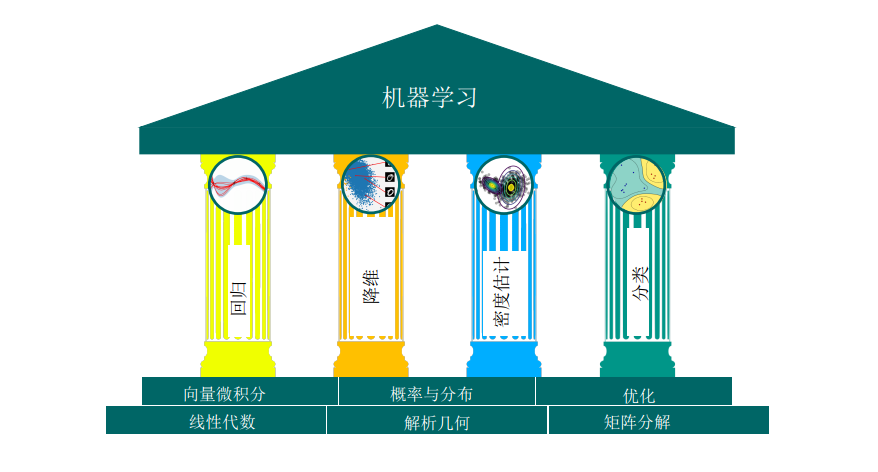
\includegraphics[width=0.92\textwidth,keepaspectratio]{docs/images/Figure1.1.png}
\caption*{\refstepcounter{figcounter}\label{fig:1-1}图~\thefigcounter 机器学习的基础和四大支柱}
\end{figure}


\emph{当然，阅读本书的方式不止两种}。 大多数读者学习使用自上而下和自下而上的方法相结合，有时在尝试更复杂的概念之前建立基本的数学技能，但也会根据机器学习的应用选择主题。

\section*{Part I 是关于数学的}
\addcontentsline{toc}{subsection}{Part I 是关于数学的}

我们在本书中介绍的机器学习的四大支柱（见图~\ref{fig:1-1}）需要扎实的数学基础，这在第一部分中进行了阐述。

我们将数值数据表示为向量，并将此类数据的表格形式表示为矩阵。 向量和矩阵的研究称为 \emph{线性代数（linear algebra）}，我们将在第2章介绍。在那里也描述了向量作为矩阵的集合。

给定代表现实世界中两个对象的两个向量，我们想对它们的相似性做出阐述。 这个想法是我们的机器学习算法（我们的预测器）应该预测相似的向量具有相似的输出。 为了形式化向量之间的相似性概念，我们需要引入将两个向量作为输入并返回表示它们相似性的数值的操作。 相似度和距离的构造是 \emph{解析几何（analytic geometry）} 的核心，将在第3章中讨论。

在第4章中，我们介绍了一些有关矩阵和 \emph{矩阵分解(matrix decomposition)} 的基本概念。 矩阵上的一些操作在机器学习中非常有用，它们允许对数据进行直观的解释和更有效的学习。

我们通常认为数据是一些真实的潜在信号的噪声观测。我们希望通过机器学习可以从噪声中识别出信号。 这要求我们有一种语言来量化“噪音”的含义。 我们通常还希望有预测器，允许我们表达某种不确定性，例如，量化我们对特定测试数据点预测值的置信度。不确定性的量化是 \emph{概率论（probability theory）} 的范畴，在第6章中有介绍。

为了训练机器学习模型，我们通常会找到最大化某些性能指标的参数。 许多优化技术需要梯度的概念，它告诉我们搜索解决方案的方向。 第 5 章是关于 \emph{向量微积分（vector calculus）} 并详细介绍梯度的概念，我们随后在第 7 章中使用它，我们将在第7章讨论 \emph{优化（optimization）} 以找到函数的最大值/最小值。

\section*{Part II 是关于机器学习的}
\addcontentsline{toc}{subsection}{Part II 是关于机器学习的}

本书的第二部分介绍了机器学习的四大支柱，如图~\ref{fig:1-1} 所示。 我们说明了本书第一部分中介绍的数学概念如何成为每个支柱的基础。 从广义上讲，章节按难度排序（升序）。

在第8章中，我们以数学方式重申机器学习的三个组成部分（数据、模型和参数估计）。此外，我们提供了一些用于构建实验设置的指南，以防止对机器学习系统的过于乐观的评估。回想一下，我们的目标是构建一个在看不见的数据上表现良好的预测器。

在第9章中，我们将仔细研究 \emph{线性回归（linear regression）}，我们的目标是找到将输入 $ \boldsymbol{x} \in \mathbb{R}^D $ 映射到对应的观测函数值 $ \boldsymbol{y} \in \mathbb{R} $ 的函数，我们可以将其解释为各自输入的标签。 我们将通过最大似然和最大后验估计以及贝叶斯线性回归来讨论经典模型拟合（参数估计），其中我们整合参数而不是优化它们。

第10章重点介绍 \emph{降维（dimensionality reduction）}，即图~\ref{fig:1-1} 中的第二个支柱，使用主成分分析。 降维的关键目标是找到高维数据 $ \boldsymbol{x} \in \mathbb{R}^D $ 的紧凑、低维表示，这通常比原始数据更容易分析。 与回归不同，降维只关心数据建模 —— 没有与数据点 $ \boldsymbol{x} $ 相关联的标签。

在第11章中，我们将转到第三个支柱：\emph{密度估计（density estimation）}。 密度估计的目标是找到描述给定数据集的概率分布。 为此，我们将专注于高斯混合模型，我们将讨论一个迭代方案来找到这个模型的参数。 与降维一样，没有与数据点 $ \boldsymbol{x} \in \mathbb{R}^D $ 相关联的标签。 但是，我们不寻求数据的低维表示。 相反，我们对描述数据的密度模型感兴趣。

第12章以深入讨论第四个支柱：\emph{分类（classification）} 来结束本书。 我们将在支持向量机的背景下讨论分类。 类似于回归（第9章），我们有输入 $ \boldsymbol{x} $ 和相应的标签 $ y $ 。 然而，与回归不同，其中标签是实值的，分类中的标签是整数，这需要特别注意。

\section*{1.3 练习和反馈}
\addcontentsline{toc}{section}{1.3 练习和反馈}
\label{sec:1.3}

我们在第一部分提供了一些练习，主要可以用纸笔完成。 对于第二部分，我们提供了编程教程（jupyter notebooks）来探索我们在本书中讨论的机器学习算法的一些特性。

我们感谢剑桥大学出版社大力支持我们实现教育和学习民主化的目标，为此本书可在以下网址免费下载 \href{https://mml-book.com}{https://mml-book.com}， 您可以在其中找到教程、勘误表和其他材料。 可以使用上述 URL 报告错误并提供反馈。

\chapter*{练习}
\addcontentsline{toc}{section}{练习}

\section*{练习 2.1}
\addcontentsline{toc}{subsection}{练习 2.1}

考虑集合与二元运算构成的代数结构 $ (\mathbb{R} \setminus \{-1\}, \star) $，其中：

\begin{equation}
a \star b := ab + a + b, \quad a, b \in \mathbb{R} \setminus \{-1\}
\tag{2.134}\label{eq:2-134}
\end{equation}

a. 证明 $ (\mathbb{R} \setminus \{-1\}, \star) $ 是一个阿贝尔群（Abelian group）。 b. 在阿贝尔群 $ (\mathbb{R} \setminus \{-1\}, \star) $ 中求解方程：

\begin{equation*}
3 \star x \star x = 15
\end{equation*}

其中 $ \star $ 的定义见式~\eqref{eq:2-134}。

\medskip\hrule\medskip

\section*{练习 2.2}
\addcontentsline{toc}{subsection}{练习 2.2}

设 $ n \in \mathbb{N} \setminus \{0\} $。设 $ k, x \in \mathbb{Z} $。我们将整数 $ k $ 的同余类（congruence class）$ \bar{k} $ 定义为集合：

\begin{equation*}
\begin{aligned}
\bar{k} &= \{x \in \mathbb{Z} \mid x - k = 0 \pmod n\} \\
&= \{x \in \mathbb{Z} \mid (\exists a \in \mathbb{Z}): (x - k = n \cdot a)\}
\end{aligned}
\end{equation*}

现在我们将所有模 $ n $ 的同余类构成的集合定义为 $ \mathbb{Z}/n\mathbb{Z} $（有时也记作 $ \mathbb{Z}_n $）。欧几里得除法（带余除法）表明该集合是一个包含 $ n $ 个元素的有限集：

\begin{equation*}
\mathbb{Z}_n = \{\bar{0}, \bar{1}, \ldots, \overline{n - 1}\}
\end{equation*}

对于所有的 $ \bar{a}, \bar{b} \in \mathbb{Z}_n $，我们定义：

\begin{equation*}
\bar{a} \oplus \bar{b} := \overline{a + b}
\end{equation*}

a. 证明 $ (\mathbb{Z}_n, \oplus) $ 是一个群。它是否是阿贝尔群？ b. 现在我们为 $ \mathbb{Z}_n $ 中的所有 $ \bar{a} $ 和 $ \bar{b} $ 定义另一个运算 $ \otimes $：

\begin{equation}
\bar{a} \otimes \bar{b} = \overline{a \times b}
\tag{2.135}\label{eq:2-135}
\end{equation}

其中 $ a \times b $ 表示 $ \mathbb{Z} $ 中的常规乘法。 令 $ n = 5 $。画出 $ \mathbb{Z}_5 \setminus \{\bar{0}\} $ 中的元素在 $ \otimes $ 运算下的乘法表（times table），即计算 $ \mathbb{Z}_5 \setminus \{\bar{0}\} $ 中所有 $ \bar{a} $ 和 $ \bar{b} $ 的乘积 $ \bar{a} \otimes \bar{b} $。 由此证明 $ \mathbb{Z}_5 \setminus \{\bar{0}\} $ 在 $ \otimes $ 运算下是封闭的，并且存在关于 $ \otimes $ 的单位元。列出 $ \mathbb{Z}_5 \setminus \{\bar{0}\} $ 中所有元素在 $ \otimes $ 运算下的逆元。由此得出结论：$ (\mathbb{Z}_5 \setminus \{\bar{0}\}, \otimes) $ 是一个阿贝尔群。 c. 证明 $ (\mathbb{Z}_8 \setminus \{\bar{0}\}, \otimes) $ 不是一个群。 d. 回顾裴蜀定理（Bézout's theorem）：两个整数 $ a $ 和 $ b $ 互素（即 $ \gcd(a, b) = 1 $），当且仅当存在两个整数 $ u $ 和 $ v $ 使得 $ au + bv = 1 $。证明 $ (\mathbb{Z}_n \setminus \{\bar{0}\}, \otimes) $ 是一个群当且仅当 $ n \in \mathbb{N} \setminus \{0\} $ 是素数。

\medskip\hrule\medskip

\section*{练习 2.3}
\addcontentsline{toc}{subsection}{练习 2.3}

考虑如下定义的 $ 3 \times 3 $ 矩阵集合 $ G $：

\begin{equation}
G = \left\{ \begin{bmatrix} 1 & x & z \\ 0 & 1 & y \\ 0 & 0 & 1 \end{bmatrix} \in \mathbb{R}^{3 \times 3} \;\middle|\; x, y, z \in \mathbb{R} \right\}
\tag{2.136}\label{eq:2-136}
\end{equation}

我们将 $ \cdot $ 定义为常规的矩阵乘法。 $ (G, \cdot) $ 是否构成一个群？如果是，它是否是阿贝尔群？请说明理由。

\medskip\hrule\medskip

\section*{练习 2.4}
\addcontentsline{toc}{subsection}{练习 2.4}

若可能，计算下列矩阵的乘积：

a.

\begin{equation*}
\begin{bmatrix} 1 & 2 \\ 4 & 5 \\ 7 & 8 \end{bmatrix} \begin{bmatrix} 1 & 1 & 0 \\ 0 & 1 & 1 \\ 1 & 0 & 1 \end{bmatrix}
\end{equation*}

b.

\begin{equation*}
\begin{adjustbox}{max width=\linewidth}
\begin{bmatrix} 1 & 2 & 3 \\ 4 & 5 & 6 \\ 7 & 8 & 9 \end{bmatrix} \begin{bmatrix} 1 & 1 & 0 \\ 0 & 1 & 1 \\ 1 & 0 & 1 \end{bmatrix}
\end{adjustbox}
\end{equation*}

c.

\begin{equation*}
\begin{adjustbox}{max width=\linewidth}
\begin{bmatrix} 1 & 1 & 0 \\ 0 & 1 & 1 \\ 1 & 0 & 1 \end{bmatrix} \begin{bmatrix} 1 & 2 & 3 \\ 4 & 5 & 6 \\ 7 & 8 & 9 \end{bmatrix}
\end{adjustbox}
\end{equation*}

d.

\begin{equation*}
\begin{bmatrix} 1 & 2 & 1 & 2 \\ 4 & 1 & -1 & -4 \end{bmatrix} \begin{bmatrix} 0 & 3 \\ 1 & -1 \\ 2 & 1 \\ 5 & 2 \end{bmatrix}
\end{equation*}

e.

\begin{equation*}
\begin{bmatrix} 0 & 3 \\ 1 & -1 \\ 2 & 1 \\ 5 & 2 \end{bmatrix} \begin{bmatrix} 1 & 2 & 1 & 2 \\ 4 & 1 & -1 & -4 \end{bmatrix}
\end{equation*}

\medskip\hrule\medskip

\section*{练习 2.5}
\addcontentsline{toc}{subsection}{练习 2.5}

求下列非齐次线性方程组 $ \boldsymbol{A} \boldsymbol{x} = \boldsymbol{b} $ 关于 $ \boldsymbol{x} $ 的所有解构成的集合 $ S $，其中 $ \boldsymbol{A} $ 和 $ \boldsymbol{b} $ 的定义分别如下：

a.

\begin{equation*}
\begin{adjustbox}{max width=\linewidth}
\boldsymbol{A} = \begin{bmatrix} 1 & 1 & -1 & -1 \\ 2 & 5 & -7 & -5 \\ 2 & -1 & 1 & 3 \\ 5 & 2 & -4 & 2 \end{bmatrix}, \quad \boldsymbol{b} = \begin{bmatrix} 1 \\ -2 \\ 4 \\ 6 \end{bmatrix}
\end{adjustbox}
\end{equation*}

b.

\begin{equation*}
\begin{adjustbox}{max width=\linewidth}
\boldsymbol{A} = \begin{bmatrix} 1 & -1 & 0 & 0 & 1 \\ 1 & 1 & 0 & -3 & 0 \\ 2 & -1 & 0 & 1 & -1 \\ -1 & 2 & 0 & -2 & -1 \end{bmatrix}, \quad \boldsymbol{b} = \begin{bmatrix} 3 \\ 6 \\ 5 \\ -1 \end{bmatrix}
\end{adjustbox}
\end{equation*}

\medskip\hrule\medskip

\section*{练习 2.6}
\addcontentsline{toc}{subsection}{练习 2.6}

使用高斯消元法，求解下列非齐次线性方程组 $ \boldsymbol{A} \boldsymbol{x} = \boldsymbol{b} $ 的所有解，其中：

\begin{equation*}
\begin{adjustbox}{max width=\linewidth}
\boldsymbol{A} = \begin{bmatrix} 0 & 1 & 0 & 0 & 1 & 0 \\ 0 & 0 & 0 & 1 & 1 & 0 \\ 0 & 1 & 0 & 0 & 0 & 1 \end{bmatrix}, \quad \boldsymbol{b} = \begin{bmatrix} 2 \\ -1 \\ 1 \end{bmatrix}
\end{adjustbox}
\end{equation*}

\medskip\hrule\medskip

\section*{练习 2.7}
\addcontentsline{toc}{subsection}{练习 2.7}

求方程组 $ \boldsymbol{A} \boldsymbol{x} = 12 \boldsymbol{x} $ 在满足 $ \sum_{i=1}^3 x_i = 1 $ 的条件下，所有解

\begin{equation*}
\boldsymbol{x} = \begin{bmatrix} x_1 \\ x_2 \\ x_3 \end{bmatrix} \in \mathbb{R}^3
\end{equation*}

，其中：

\begin{equation*}
\boldsymbol{A} = \begin{bmatrix} 6 & 4 & 3 \\ 6 & 0 & 9 \\ 0 & 8 & 0 \end{bmatrix}
\end{equation*}

\medskip\hrule\medskip

\section*{练习 2.8}
\addcontentsline{toc}{subsection}{练习 2.8}

若可能，求下列矩阵的逆矩阵：

a.

\begin{equation*}
\boldsymbol{A} = \begin{bmatrix} 2 & 3 & 4 \\ 3 & 4 & 5 \\ 4 & 5 & 6 \end{bmatrix}
\end{equation*}

b.

\begin{equation*}
\begin{adjustbox}{max width=\linewidth}
\boldsymbol{A} = \begin{bmatrix} 1 & 0 & 1 & 0 \\ 0 & 1 & 1 & 0 \\ 1 & 1 & 0 & 1 \\ 1 & 1 & 1 & 0 \end{bmatrix}
\end{adjustbox}
\end{equation*}

\medskip\hrule\medskip

\section*{练习 2.9}
\addcontentsline{toc}{subsection}{练习 2.9}

下列哪些集合是 $ \mathbb{R}^3 $ 的子空间？

a. $ A = \{(\lambda, \lambda + \mu^3, \lambda - \mu^3) \mid \lambda, \mu \in \mathbb{R}\} $ b. $ B = \{(\lambda^2, -\lambda^2, 0) \mid \lambda \in \mathbb{R}\} $ c. 设 $ \gamma \in \mathbb{R} $，

\begin{equation*}
C = \{(\xi_1, \xi_2, \xi_3) \in \mathbb{R}^3 \mid \xi_1 - 2\xi_2 + 3\xi_3 = \gamma\}
\end{equation*}

d. $ D = \{(\xi_1, \xi_2, \xi_3) \in \mathbb{R}^3 \mid \xi_2 \in \mathbb{Z}\} $

\medskip\hrule\medskip

\section*{练习 2.10}
\addcontentsline{toc}{subsection}{练习 2.10}

下列向量集合是否线性无关？

a.

\begin{equation*}
\boldsymbol{x}_1 = \begin{bmatrix} 2 \\ -1 \\ 3 \end{bmatrix}, \quad \boldsymbol{x}_2 = \begin{bmatrix} 1 \\ 1 \\ -2 \end{bmatrix}, \quad \boldsymbol{x}_3 = \begin{bmatrix} 3 \\ -3 \\ 8 \end{bmatrix}
\end{equation*}

b.

\begin{equation*}
\begin{adjustbox}{max width=\linewidth}
\boldsymbol{x}_1 = \begin{bmatrix} 1 \\ 2 \\ 1 \\ 0 \\ 0 \end{bmatrix}, \quad \boldsymbol{x}_2 = \begin{bmatrix} 1 \\ 1 \\ 0 \\ 1 \\ 1 \end{bmatrix}, \quad \boldsymbol{x}_3 = \begin{bmatrix} 1 \\ 0 \\ 0 \\ 1 \\ 1 \end{bmatrix}
\end{adjustbox}
\end{equation*}

\medskip\hrule\medskip

\section*{练习 2.11}
\addcontentsline{toc}{subsection}{练习 2.11}

将向量

\begin{equation*}
\boldsymbol{y} = \begin{bmatrix} 1 \\ -2 \\ 5 \end{bmatrix}
\end{equation*}

表示为下列向量的线性组合：

\begin{equation*}
\boldsymbol{x}_1 = \begin{bmatrix} 1 \\ 1 \\ 1 \end{bmatrix}, \quad \boldsymbol{x}_2 = \begin{bmatrix} 1 \\ 2 \\ 3 \end{bmatrix}, \quad \boldsymbol{x}_3 = \begin{bmatrix} 2 \\ -1 \\ 1 \end{bmatrix}
\end{equation*}

\medskip\hrule\medskip

\section*{练习 2.12}
\addcontentsline{toc}{subsection}{练习 2.12}

考虑 $ \mathbb{R}^4 $ 的两个子空间：

\begin{equation*}
\begin{adjustbox}{max width=\linewidth}
U_1 = \operatorname{span}\left[ \begin{bmatrix} 1 \\ 1 \\ -3 \\ 1 \end{bmatrix}, \begin{bmatrix} 2 \\ -1 \\ 0 \\ -1 \end{bmatrix}, \begin{bmatrix} -1 \\ 1 \\ -1 \\ 1 \end{bmatrix} \right], \quad U_2 = \operatorname{span}\left[ \begin{bmatrix} -1 \\ -2 \\ 2 \\ 1 \end{bmatrix}, \begin{bmatrix} 2 \\ -2 \\ 0 \\ 0 \end{bmatrix}, \begin{bmatrix} -3 \\ 6 \\ -2 \\ -1 \end{bmatrix} \right]
\end{adjustbox}
\end{equation*}

求 $ U_1 \cap U_2 $ 的一组基。

\medskip\hrule\medskip

\section*{练习 2.13}
\addcontentsline{toc}{subsection}{练习 2.13}

考虑两个子空间 $ U_1 $ 和 $ U_2 $，其中 $ U_1 $ 是齐次线性方程组 $ \boldsymbol{A}_1 \boldsymbol{x} = \boldsymbol{0} $ 的解空间，$ U_2 $ 是齐次线性方程组 $ \boldsymbol{A}_2 \boldsymbol{x} = \boldsymbol{0} $ 的解空间，且：

\begin{equation*}
\begin{adjustbox}{max width=\linewidth}
\boldsymbol{A}_1 = \begin{bmatrix} 1 & 0 & 1 & 1 \\ -2 & -1 & 2 & 1 \\ 3 & 1 & 0 & 1 \end{bmatrix}, \quad \boldsymbol{A}_2 = \begin{bmatrix} 3 & -3 & 0 & 1 \\ 2 & 3 & 7 & -5 \\ 2 & 3 & -1 & 2 \end{bmatrix}
\end{adjustbox}
\end{equation*}

a. 确定 $ U_1, U_2 $ 的维度。 b. 确定 $ U_1 $ 和 $ U_2 $ 的基。 c. 确定 $ U_1 \cap U_2 $ 的一组基。

\medskip\hrule\medskip

\section*{练习 2.14}
\addcontentsline{toc}{subsection}{练习 2.14}

考虑两个子空间 $ U_1 $ 和 $ U_2 $，其中 $ U_1 $ 由 $ \boldsymbol{A}_1 $ 的列向量张成，$ U_2 $ 由 $ \boldsymbol{A}_2 $ 的列向量张成，且：

\begin{equation*}
\begin{adjustbox}{max width=\linewidth}
\boldsymbol{A}_1 = \begin{bmatrix} 1 & 0 & 1 & 1 \\ -2 & -1 & 2 & 1 \\ 3 & 1 & 0 & 1 \end{bmatrix}, \quad \boldsymbol{A}_2 = \begin{bmatrix} 3 & -3 & 0 & 1 \\ 2 & 3 & 7 & -5 \\ 2 & 3 & -1 & 2 \end{bmatrix}
\end{adjustbox}
\end{equation*}

a. 确定 $ U_1, U_2 $ 的维度。 b. 确定 $ U_1 $ 和 $ U_2 $ 的基。 c. 确定 $ U_1 \cap U_2 $ 的一组基。

\medskip\hrule\medskip

\section*{练习 2.15}
\addcontentsline{toc}{subsection}{练习 2.15}

设 $ F = \{(x, y, z) \in \mathbb{R}^3 \mid x + y - z = 0\} $ 且 $ G = \{(a - b, a + b, a - 3b) \mid a, b \in \mathbb{R}\} $。

a. 证明 $ F $ 和 $ G $ 是 $ \mathbb{R}^3 $ 的子空间。 b. 在不借助任何基向量的前提下，计算 $ F \cap G $。 c. 分别找出 $ F $ 和 $ G $ 的一组基，利用前面求得的基向量计算 $ F \cap G $，并将结果与上一问进行比对验证。

\medskip\hrule\medskip

\section*{练习 2.16}
\addcontentsline{toc}{subsection}{练习 2.16}

下列映射是否为线性映射？

a. 设 $ a, b \in \mathbb{R} $。

\begin{equation*}
\begin{aligned}
\Phi : L^1([a, b]) &\to \mathbb{R} \\
f &\mapsto \Phi(f) = \int_a^b f(x)\,\mathrm{d}x
\end{aligned}
\end{equation*}

其中 $ L^1([a, b]) $ 表示 $ [a, b] $ 上的可积函数集合。

b.

\begin{equation*}
\begin{aligned}
\Phi : C^1 &\to C^0 \\
f &\mapsto \Phi(f) = f'
\end{aligned}
\end{equation*}

其中对 $ k \geqslant 1 $，$ C^k $ 表示 $ k $ 阶连续可微函数集合，而 $ C^0 $ 表示连续函数集合。

c.

\begin{equation*}
\begin{aligned}
\Phi : \mathbb{R} &\to \mathbb{R} \\
x &\mapsto \Phi(x) = \cos(x)
\end{aligned}
\end{equation*}

d.

\begin{equation*}
\begin{aligned}
\Phi : \mathbb{R}^3 &\to \mathbb{R}^2 \\
\boldsymbol{x} &\mapsto \begin{bmatrix} 1 & 2 & 3 \\ 1 & 4 & 3 \end{bmatrix} \boldsymbol{x}
\end{aligned}
\end{equation*}

e. 设 $ \theta \in [0, 2\pi) $。

\begin{equation*}
\begin{aligned}
\Phi : \mathbb{R}^2 &\to \mathbb{R}^2 \\
\boldsymbol{x} &\mapsto \begin{bmatrix} \cos(\theta) & \sin(\theta) \\ -\sin(\theta) & \cos(\theta) \end{bmatrix} \boldsymbol{x}
\end{aligned}
\end{equation*}

\medskip\hrule\medskip

\section*{练习 2.17}
\addcontentsline{toc}{subsection}{练习 2.17}

考虑线性映射：

\begin{equation*}
\begin{adjustbox}{max width=\linewidth}
\begin{aligned}
\Phi : \mathbb{R}^3 &\to \mathbb{R}^4 \\
\Phi\left(\begin{bmatrix} x_1 \\ x_2 \\ x_3 \end{bmatrix}\right) &= \begin{bmatrix} 3x_1 + 2x_2 + x_3 \\ x_1 + x_2 + x_3 \\ x_1 - 3x_2 \\ 2x_1 + 3x_2 + x_3 \end{bmatrix}
\end{aligned}
\end{adjustbox}
\end{equation*}

求变换矩阵 $ \boldsymbol{A}_{\Phi} $。 确定 $ \operatorname{rk}(\boldsymbol{A}_{\Phi}) $。 计算 $ \Phi $ 的核（kernel，零空间）与像（image）。$ \operatorname{dim}(\operatorname{ker}(\Phi)) $ 和 $ \operatorname{dim}(\operatorname{Im}(\Phi)) $ 分别是多少？

\medskip\hrule\medskip

\section*{练习 2.18}
\addcontentsline{toc}{subsection}{练习 2.18}

设 $ E $ 为一个向量空间。设 $ f $ 和 $ g $ 为 $ E $ 上的两个自同态（automorphisms，注：亦作自同构），满足 $ f \circ g = \operatorname{id}_E $（即 $ f \circ g $ 为恒等映射 $ \operatorname{id}_E $）。证明：

\begin{equation*}
\operatorname{ker}(f) = \operatorname{ker}(g \circ f), \quad \operatorname{Im}(g) = \operatorname{Im}(g \circ f), \quad \operatorname{ker}(f) \cap \operatorname{Im}(g) = \{\boldsymbol{0}_E\}
\end{equation*}

\medskip\hrule\medskip

\section*{练习 2.19}
\addcontentsline{toc}{subsection}{练习 2.19}

考虑一个自同态 $ \Phi : \mathbb{R}^3 \to \mathbb{R}^3 $，其关于 $ \mathbb{R}^3 $ 标准基的变换矩阵为：

\begin{equation*}
\boldsymbol{A}_{\Phi} = \begin{bmatrix} 1 & 1 & 0 \\ 1 & -1 & 0 \\ 1 & 1 & 1 \end{bmatrix}
\end{equation*}

\begin{enumerate}
\item 确定 $ \operatorname{ker}(\Phi) $ 和 $ \operatorname{Im}(\Phi) $。  
\item 确定 $ \Phi $ 关于基 $ B $ 的变换矩阵 $ \tilde{\boldsymbol{A}}_{\Phi} $，其中：
\end{enumerate}

\begin{equation*}
B = \left( \begin{bmatrix} 1 \\ 1 \\ 1 \end{bmatrix}, \begin{bmatrix} 1 \\ 2 \\ 1 \end{bmatrix}, \begin{bmatrix} 1 \\ 0 \\ 0 \end{bmatrix} \right)
\end{equation*}

即执行向新基 $ B $ 的基变换。

\medskip\hrule\medskip

\section*{练习 2.20}
\addcontentsline{toc}{subsection}{练习 2.20}

考虑在 $ \mathbb{R}^2 $ 标准基下表示的 4 个向量：

\begin{equation*}
\begin{adjustbox}{max width=\linewidth}
\boldsymbol{b}_1 = \begin{bmatrix} 2 \\ 1 \end{bmatrix}, \quad \boldsymbol{b}_2 = \begin{bmatrix} -1 \\ -1 \end{bmatrix}, \quad \boldsymbol{b}'_1 = \begin{bmatrix} 2 \\ -2 \end{bmatrix}, \quad \boldsymbol{b}'_2 = \begin{bmatrix} 1 \\ 1 \end{bmatrix}
\end{adjustbox}
\end{equation*}

定义 $ \mathbb{R}^2 $ 的两个有序基 $ B = (\boldsymbol{b}_1, \boldsymbol{b}_2) $ 和 $ B' = (\boldsymbol{b}'_1, \boldsymbol{b}'_2) $。

\begin{enumerate}
\item 证明 $ B $ 和 $ B' $ 是 $ \mathbb{R}^2 $ 的两组基，并画出这些基向量。  
\item 计算实现从 $ B' $ 到 $ B $ 基变换的矩阵 $ \boldsymbol{P}_1 $。  
\item 考虑在 $ \mathbb{R}^3 $ 标准基下定义的 3 个向量：
\end{enumerate}

\begin{equation*}
\boldsymbol{c}_1 = \begin{bmatrix} 1 \\ 2 \\ -1 \end{bmatrix}, \quad \boldsymbol{c}_2 = \begin{bmatrix} 0 \\ -1 \\ 2 \end{bmatrix}, \quad \boldsymbol{c}_3 = \begin{bmatrix} 1 \\ 0 \\ -1 \end{bmatrix}
\end{equation*}

定义 $ C = (\boldsymbol{c}_1, \boldsymbol{c}_2, \boldsymbol{c}_3) $。

a. 证明 $ C $ 是 $ \mathbb{R}^3 $ 的一组基，例如通过计算行列式（参见第 4.1 节）。 b. 记 $ C' = (\boldsymbol{c}'_1, \boldsymbol{c}'_2, \boldsymbol{c}'_3) $ 为 $ \mathbb{R}^3 $ 的标准基。求实现从 $ C $ 到 $ C' $ 基变换的矩阵 $ \boldsymbol{P}_2 $。

\begin{enumerate}
\item 考虑同态 $ \Phi : \mathbb{R}^2 \to \mathbb{R}^3 $，满足：
\end{enumerate}

\begin{equation*}
\begin{aligned}
\Phi(\boldsymbol{b}_1 + \boldsymbol{b}_2) &= \boldsymbol{c}_2 + \boldsymbol{c}_3 \\
\Phi(\boldsymbol{b}_1 - \boldsymbol{b}_2) &= 2\boldsymbol{c}_1 - \boldsymbol{c}_2 + 3\boldsymbol{c}_3
\end{aligned}
\end{equation*}

其中 $ B = (\boldsymbol{b}_1, \boldsymbol{b}_2) $ 与 $ C = (\boldsymbol{c}_1, \boldsymbol{c}_2, \boldsymbol{c}_3) $ 分别是 $ \mathbb{R}^2 $ 和 $ \mathbb{R}^3 $ 的有序基。 确定 $ \Phi $ 关于有序基 $ B $ 与 $ C $ 的变换矩阵 $ \boldsymbol{A}_{\Phi} $。

\begin{enumerate}
\item 确定 $ \Phi $ 关于基 $ B' $ 与 $ C' $ 的变换矩阵 $ \boldsymbol{A}' $。  
\item 考虑在基 $ B' $ 下坐标为 $ [2, 3]^\top $ 的向量 $ \boldsymbol{x} \in \mathbb{R}^2 $，换言之，$ \boldsymbol{x} = 2\boldsymbol{b}'_1 + 3\boldsymbol{b}'_2 $。
\end{enumerate}

a. 计算 $ \boldsymbol{x} $ 在基 $ B $ 下的坐标。 b. 据此计算 $ \Phi(\boldsymbol{x}) $ 在基 $ C $ 下表示的坐标。 c. 随后，用 $ \boldsymbol{c}'_1, \boldsymbol{c}'_2, \boldsymbol{c}'_3 $ 表示 $ \Phi(\boldsymbol{x}) $。 d. 利用 $ \boldsymbol{x} $ 在 $ B' $ 下的表示以及矩阵 $ \boldsymbol{A}' $ 直接求出上述结果。

\chapter*{线性代数}
\addcontentsline{toc}{section}{线性代数}


\begin{figure}[H]
\centering
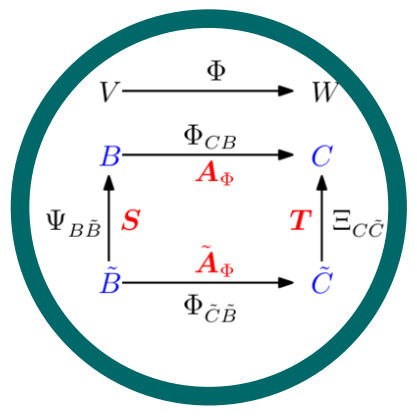
\includegraphics[width=320pt,keepaspectratio]{docs/images/LinearAlgebra.png}
\caption*{线性代数 LinearA lgebra}
\end{figure}


在形式化直观概念时，一种常见的方法是构造一组对象（符号）和一组操作这些对象的规则。 这被称为 \emph{代数（algebra）} 。线性代数是研究向量和某些代数规则来操作向量。 我们很多人在学校知道的向量被称为“几何向量”，通常用字母上方的小箭头表示，例如 $ \vec{x} $ 和 $ \vec{y} $ 。 在本书中，我们讨论向量的更一般概念并使用粗体字母表示它们，例如 $ \boldsymbol{x} $ 和 $ \boldsymbol{y} $ 。

通常，向量是特殊的对象，可以将它们相加并乘以标量以产生另一个相同类型的对象。 从抽象的数学角度来看，任何满足这两个属性的对象都可以被认为是一个向量。 以下是此类向量对象的一些示例：

\begin{enumerate}
\item 几何向量（Geometric vectors）。 这个向量的例子可能在高中数学和物理中很熟悉。 几何向量 — 参见图~\ref{fig:2-1}(a) — 是有向线段，可以绘制（至少在二维中）。 几何向量可以相加，比如 $ \vec{x} +  \vec{y} = \vec{z} $ 是另外一个几何向量。此外，乘以标量 $ \lambda\vec{x} $，$ \lambda \in \mathbb{R} $，也是一个几何向量。实际上，它是由 $ \lambda $ 缩放的原始向量。 因此，几何向量是前面介绍的向量概念的实例。 将向量解释为几何向量，可以让我们能够利用对方向和大小的直觉来推理数学运算。
\end{enumerate}


\begin{figure}[H]
\centering
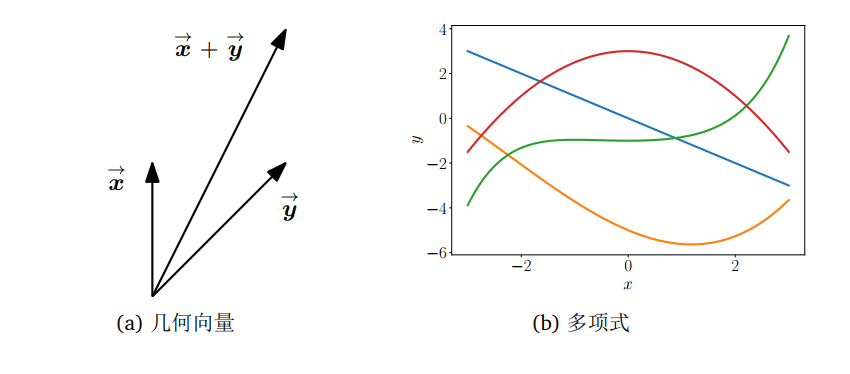
\includegraphics[width=0.92\textwidth,keepaspectratio]{docs/images/Figure2.1.png}
\caption*{\refstepcounter{figcounter}\label{fig:2-1}图~\thefigcounter 不同类型的向量。 向量可以是令人惊讶的对象，包括 (a) 几何向量和 (b) 多项式。}
\end{figure}


\begin{enumerate}
\item 多项式（Polynomials）也是向量；参见图~\ref{fig:2-1}(b)：两个多项式可以相加，得到另一个多项式； 并且它们可以乘以一个标量 $ \lambda \in \mathbb{R} $，结果也是一个多项式。 因此，多项式是（相当不寻常的）向量的实例。 请注意，多项式与几何向量非常不同。 几何向量是具体的“图画”，多项式是抽象的概念。 然而，它们都是前述意义上的向量。
\end{enumerate}

\begin{enumerate}
\item 音频信号（Audio signals）是向量。 音频信号表示为一系列数字。 我们可以将音频信号加在一起，它们的总和就是一个新的音频信号。 如果我们缩放音频信号，我们也会获得音频信号。 因此，音频信号也是一种向量。
\end{enumerate}

\begin{enumerate}
\item $ \mathbb{R}^n $（n 个实数的元组）的元素是向量。  $ \mathbb{R}^n $ 比多项式更抽象，它是我们在本书中关注的概念。例如，
\end{enumerate}

\begin{equation}
\boldsymbol{a} = \begin{bmatrix} 1 \\ 2 \\ 3 \\ \end{bmatrix} \in \mathbb{R}^3
\tag{2.1}\label{eq:2-1}
\end{equation}

是一个三元组数字的例子。将两个向量 $ \boldsymbol{a}, \boldsymbol{b} \in \mathbb{R}^n $ 按分量相加得到另一个向量：$ \boldsymbol{a} + \boldsymbol{b} = \boldsymbol{c} \in \mathbb{R}^n $。此外，将 $ \boldsymbol{a} \in \mathbb{R}^n $ 乘以 $ \lambda \in \mathbb{R} $ 得到一个缩放向量 $ \lambda \boldsymbol{a} \in \mathbb{R}^n $。将向量视为 $ \mathbb{R}^n $ 的元素有一个额外的好处，它松散地对应于计算机上的实数数组。 许多编程语言支持数组操作，这允许方便地实现涉及向量操作的算法。

线性代数侧重于这些向量概念之间的相似性。 我们可以将它们加在一起并乘以标量。 我们将主要关注 $ \mathbb{R}^n $ 中的向量，因为线性代数中的大多数算法都是在 $ \mathbb{R}^n $ 中制定的。 我们将在第8章中看到，我们经常将数据表示为 $ \mathbb{R}^n $ 中的向量。 在本书中，我们将关注有限维向量空间，在这种情况下，任何类型的向量和 $ \mathbb{R}^n $ 之间都存在 1:1 的对应关系。 方便时，我们将使用有关几何向量的直觉并考虑基于数组的算法。

数学中的一个主要思想是“闭包（closure）”的思想。 这就是问题：我提议的行动会产生什么样的结果？ 在向量的情况下：从一个小的向量集开始，将它们相加并缩放它们，可以得到什么样的向量集？这就产生了向量空间（第2.4节）。向量空间的概念及其性质是机器学习的基础。本章介绍的概念如图~\ref{fig:2-2}所示。

本章主要基于 Drumm 和 Weil (2001)、Strang (2003)、Hogben (2013)、Liesen 和 Mehrmann (2015) 的讲义和书籍，以及 Pavel Grinfeld 的线性代数系列。 其他优秀资源包括 Gilbert Strang 在麻省理工学院的线性代数课程和 3Blue1Brown 的线性代数系列。


\begin{figure}[H]
\centering
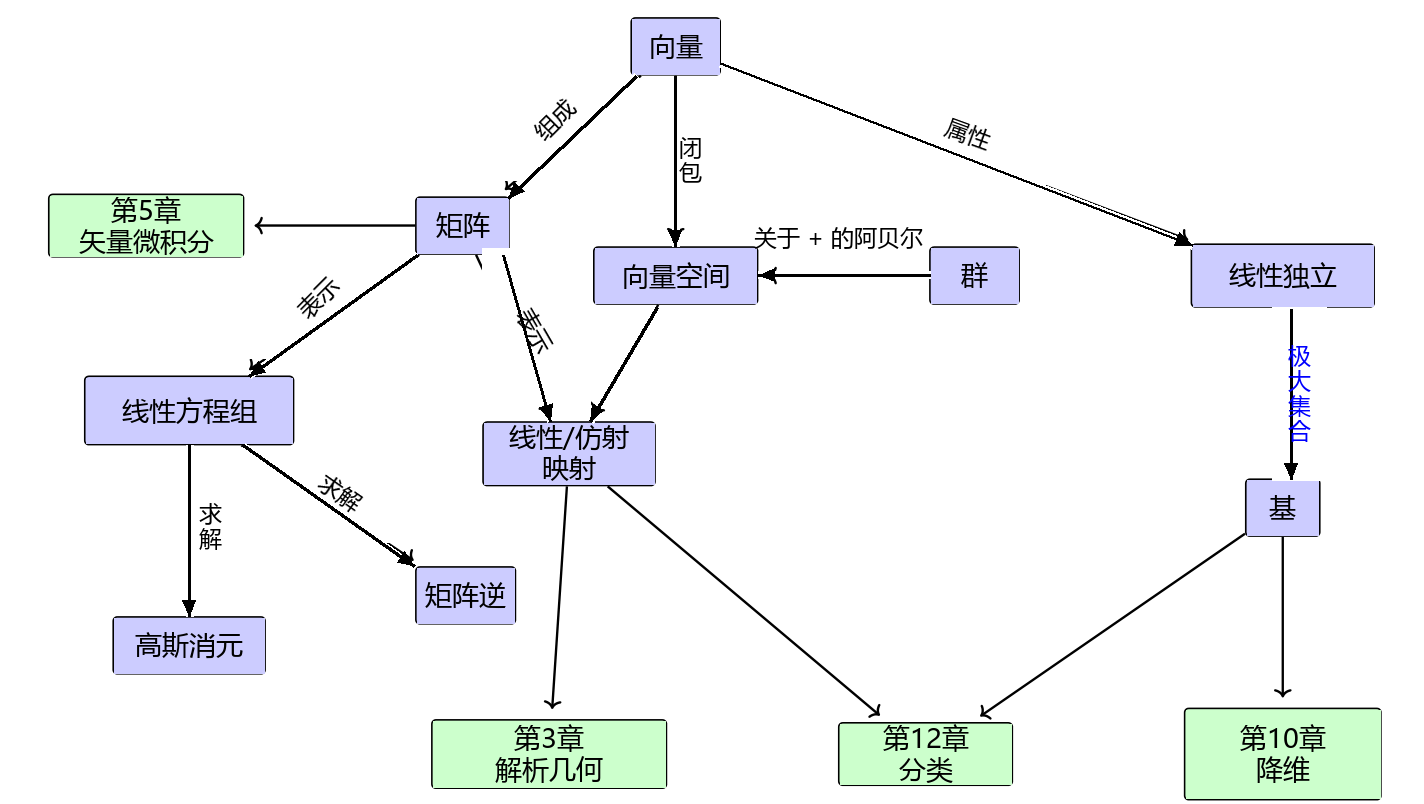
\includegraphics[width=0.92\textwidth,keepaspectratio]{docs/images/Figure2.2.png}
\caption*{\refstepcounter{figcounter}\label{fig:2-2}图~\thefigcounter 本章介绍的概念的思维导图，以及它们在本书其他部分中的使用位置。}
\end{figure}


线性代数在机器学习和普通数学中扮演着重要的角色。 本章介绍的概念进一步扩展到第3章中的几何概念。在第5章中，我们将讨论向量微积分，其中矩阵运算的基本知识是必不可少的。 在第10章中，我们将使用投影（将在第 3.8 节中介绍）通过主成分分析（PCA）进行降维。 在第9章中，我们将讨论线性回归，其中线性代数在解决最小二乘问题中起着核心作用。

\section*{2.1 线性方程组}
\addcontentsline{toc}{section}{2.1 线性方程组}
\label{sec:2.1}

线性方程组是线性代数的核心部分。 许多问题可以表述为线性方程组，而线性代数为我们提供了解决它们的工具。

\begin{notebox}
\textbf{例 2.1}
\end{notebox}

\begin{notebox}
公司生产的产品 $ N_1,...,N_n $ 需要原材料 $ R_1,...,R_m $。为了生产一个单位的产品 $ N_j $，需要 $ a_{ij} $ 个单位的资源 $ R_i $，其中 $ i = 1,...,m $ 且 $ j = 1,...,n $。目标是找到一个最佳生产计划，即如果总共有 $ b_i $ 个单位的资源 $ R_i $ 可用并且（理想情况下）没有剩余资源，则应该生产多少单位 $ x_j $ 的产品 $ N_j $。
\end{notebox}

\begin{notebox}
如果我们生产 $ x_1,...,x_n $ 个单位对应的产品，我们一共需要

\begin{equation}
a_{i1}x_1 + \cdots + a_{in}x_n
\tag{2.2}\label{eq:2-2}
\end{equation}

个单位的资源 $ R_i $。因此，最优生产计划 $ (x_1,...,x_n) \in \mathbb{R}^n $ 必须满足以下方程组：

\begin{equation}
\begin{array}{clr}
  a_{11}x_1 + \cdots + a_{1n}x_n & = b_1 \\
        & \vdots \\
  a_{m1}x_1 +  \cdots + a_{mn}x_n & = b_m
\end{array}
\tag{2.3}\label{eq:2-3}
\end{equation}

其中 $ a_{ij} \in \mathbb{R} $ 和 $ b_i \in \mathbb{R} $。
\end{notebox}

\begin{notebox}
方程 (2.3) 是线性方程组（system of linear equations）的一般形式，$ x_1,...,x_n $ 是这个系统的未知数。满足 (2.3) 的每一个 n 元组 $ (x_1,...,x_n) \in \mathbb{R}^n $ 都是线性方程组的一个解。
\end{notebox}

\begin{notebox}
\textbf{例 2.2}
\end{notebox}

\begin{notebox}
线性方程组：

\begin{equation}
\begin{array}{clr}
  x_1 + x_2 + x_3 & = 3 &(1)\\
  x_1 - x_2 + 2x_3 & = 2 &(2)\\
  2x_1 + 3x_3 & = 1 &(3)
\end{array}
\tag{2.4}\label{eq:2-4}
\end{equation}

\emph{没有解} ：将前两个方程相加得到 $ 2x_1 + 3x_3 = 5 $，这与第三个方程相矛盾。
\end{notebox}

\begin{notebox}
让我们看看线性方程组：

\begin{equation}
\begin{array}{clr}
  x_1 + x_2 + x_3 & = 3 &(1)\\
  x_1 - x_2 + 2x_3 & = 2 &(2)\\
  x_2 + x_3 & = 2 &(3)
\end{array}
\tag{2.5}\label{eq:2-5}
\end{equation}

从第一个和第三个等式可以得出 $ x_1 = 1 $。从（1）+（2），我们得到 $ 2x_1 + 3x_3 = 5 $，即 $ x_3 = 1 $。从 (3) 中，我们得到 $ x_2 = 1 $。因此，(1,1,1) 是唯一可能且 \emph{唯一的解} （通过代入验证 (1,1,1) 是解）。
\end{notebox}

\begin{notebox}
作为第三个例子，我们考虑：

\begin{equation}
\begin{array}{clr}
  x_1 + x_2 + x_3 & = 3 &(1)\\
  x_1 - x_2 + 2x_3 & = 2 &(2)\\
  2x_1 + 3x_3 & = 5 &(3)
\end{array}
\tag{2.6}\label{eq:2-6}
\end{equation}

由于（1）+（2）=（3），我们可以省略第三个方程（冗余）。从（1）和（2），我们得到 $ 2x_1 = 5 - 3x_3 $ 和 $ 2x_2 = 1 + x_3 $。我们定义 $ x_3 = a \in \mathbb{R} $ 作为一个自由变量，使得任何三元组：

\begin{equation}
\left( \frac{5}{2} - \frac{3}{2}a, \frac{1}{2} + \frac{1}{2}a, a \right), a \in \mathbb{R}
\tag{2.7}\label{eq:2-7}
\end{equation}

都是线性方程组的解，即我们得到一个包含无限多个解的解集。
\end{notebox}


\begin{figure}[H]
\centering
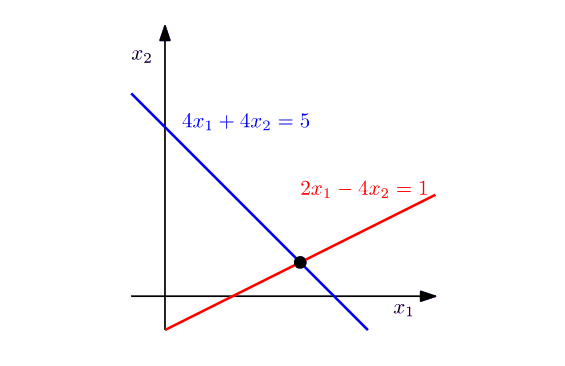
\includegraphics[width=0.92\textwidth,keepaspectratio]{docs/images/Figure2.3.png}
\caption*{\refstepcounter{figcounter}\label{fig:2-3}图~\thefigcounter 具有两个变量的两个线性方程组的解空间可以在几何上解释为两条线的交点。 每个线性方程代表一条线。}
\end{figure}


一般而言，对于实值线性方程组，我们要么没有，只有一个，要么有无穷多个解。 当我们无法求解线性方程组时，线性回归（第9章）是解决例2.1的一个版本。

\emph{备注} （线性方程组的几何解释）。 在具有两个变量 $ x_1, x_2 $ 的线性方程组中，每个线性方程定义 $ x_1 x_2 $ 平面上的一条线。 由于线性方程组的解必须同时满足所有方程，因此解集是这些线的交点。 该交集可以是一条线（如果线性方程描述同一条线）、一个点或空（当这些线平行时）。 图~\ref{fig:2-3} 给出了方程组

\begin{equation}
\begin{array}{clr}
  4x_1 + 4x_2 & = 5 \\
  2x_1 - 4x_2 & = 1
\end{array}
\tag{2.8}\label{eq:2-8}
\end{equation}

的说明，其中解空间是点 $ (x_1, x_2) = (1, \frac{1}{4}) $。 类似地，对于三个变量，每个线性方程确定三维空间中的一个平面。 当我们与这些平面相交时，即同时满足所有线性方程，我们可以得到一个解集，它是一个平面、一条线、一个点或空的（当这些平面没有公共交点时）。

对于求解线性方程组的系统方法，我们将引入一个有用的紧凑符号。 我们将系数 $ a_{ij} $ 收集到向量中并将向量收集到矩阵中。 换句话说，我们按照以下形式编写（2.3）中的系统：

\begin{equation}
\begin{adjustbox}{max width=\linewidth}
\begin{bmatrix} a_{11} \\ \vdots \\ a_{m1} \end{bmatrix}x_1 + 
 \begin{bmatrix} a_{12} \\ \vdots \\ a_{m2} \end{bmatrix}x_2 + 
 \cdots + 
 \begin{bmatrix} a_{1n} \\ \vdots \\ a_{mn} \end{bmatrix}x_n = 
 \begin{bmatrix} b_1 \\ \vdots \\ b_m \end{bmatrix}
\end{adjustbox}
\tag{2.9}\label{eq:2-9}
\end{equation}

\begin{equation}
\Longleftrightarrow 
\begin{bmatrix} a_{11} & \cdots & a_{1n} \\ \vdots \\ a_{m1} & \cdots & a_{mn} \end{bmatrix} 
\begin{bmatrix} x_1 \\ \vdots \\ x_n \end{bmatrix} = 
\begin{bmatrix} b_1 \\ \vdots \\ b_m \end{bmatrix}
\tag{2.10}\label{eq:2-10}
\end{equation}

下面，我们将仔细研究这些矩阵并定义计算规则。 我们将在2.3节返回求解线性方程。

\section*{2.2 矩阵}
\addcontentsline{toc}{section}{2.2 矩阵}
\label{sec:2.2}

矩阵在线性代数中起着核心作用。 它们可用于紧凑地表示线性方程组，此外它们也表示线性函数（线性映射），我们将在后面的2.7节中看到。 在我们讨论这些有趣的话题之前，让我们首先定义矩阵是什么以及我们可以对矩阵进行什么样的操作。 我们将在第4章看到更多矩阵的性质。

\textbf{定义 2.1} （矩阵）。对于 $ m,n \in \mathbb{N} $，实值 $ (m,n) $ \emph{矩阵（matrix）} $ \boldsymbol{A} $ 是元素 $ a_{ij} $ 的 $ m·n $ 元组，$ i = 1,...,m , j = 1,...,n $，其由$ m $行和$ n $列组成的矩形排序阵列：

\begin{equation}
\begin{adjustbox}{max width=\linewidth}
\boldsymbol{A} = \begin{bmatrix} a_{11} & a_{12} & \cdots & a_{1n} \\ a_{21} & a_{22} & \cdots & a_{2n} \\ \vdots & \vdots & & \vdots \\ a_{m1} & a_{m2} & \cdots & a_{mn} \end{bmatrix}, a_{ij} \in \mathbb{R}.
\end{adjustbox}
\tag{2.11}\label{eq:2-11}
\end{equation}

通常 $ (1,n) $ - 矩阵称为行，$ (m,1) $ - 矩阵称为列。 这些特殊矩阵也称为 \emph{行/列向量（row/column vectors）} 。

$ \mathbb{R}^{m \times n} $ 是所有实值 $ (m,n) $ 矩阵的集合。 $ \boldsymbol{A} \in \mathbb{R}^{m \times n} $ 可以等价的表示为将矩阵的所有 $ n $ 列堆叠成一个长的向量 $ \boldsymbol{a} \in \mathbb{R}^{mn} $ ； 见图~\ref{fig:2-4}。


\begin{figure}[H]
\centering
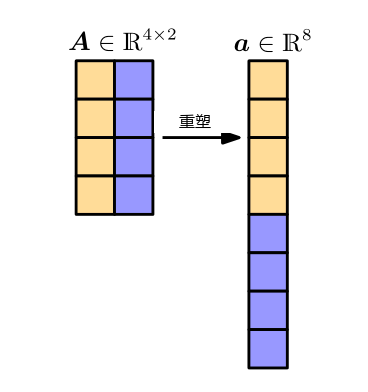
\includegraphics[width=320pt,keepaspectratio]{docs/images/Figure2.4.png}
\caption*{\refstepcounter{figcounter}\label{fig:2-4}图~\thefigcounter 通过堆叠其列，矩阵A可以表示为一个长向量a}
\end{figure}


\section*{2.2.1 矩阵加法和乘法}
\addcontentsline{toc}{subsection}{2.2.1 矩阵加法和乘法}

两个矩阵的和 $ \boldsymbol{A} \in \mathbb{R}^{m \times n}, \boldsymbol{B} \in \mathbb{R}^{m \times n} $ 被定义为对应元素的和，即，

\begin{equation}
\boldsymbol{A} + \boldsymbol{B} := \begin{bmatrix} a_{11} + b_{11} & \cdots & a_{1n} + b_{1n} \\ \vdots \\ a_{m1} + b_{m1} & \cdots & a_{mn} + b_{mn} \end{bmatrix} \in \mathbb{R}^{m \times n}
\tag{2.12}\label{eq:2-12}
\end{equation}

对于矩阵 $ \boldsymbol{A} \in \mathbb{R}^{m \times n}, \boldsymbol{B} \in \mathbb{R}^{n \times k} $ ，乘积 $ \boldsymbol{C} = \boldsymbol{A} \boldsymbol{B} \in \mathbb{R}^{m \times k} $ 的元素 $ c_{ij} $ 计算自

\begin{equation}
c_{ij} = \sum_{l=1}^{n}{a_{il}b_{lj}}, i = 1,...,m, \ j = 1,...,k
\tag{2.13}\label{eq:2-13}
\end{equation}

\begin{notebox}
注意矩阵的大小。
\end{notebox}

这意味着，为了计算元素 $ c_{ij} $，我们将 $ \boldsymbol{A} $ 的第 $ i $ 行的元素与 $ \boldsymbol{B} $ 的第 $ j $ 列的元素相乘，然后将它们相加。 稍后在第3.2节中，我们将称其为相应行和列的 \emph{点积（dot produc）} 。 在需要明确表示正在执行乘法的情况下，我们使用符号 $ \boldsymbol{A} \ · \boldsymbol{B} $  来表示乘法（明确显示“·”）。

\begin{notebox}
$ \boldsymbol{A} $ 中有 $ n $ 列，$ \boldsymbol{B} $ 中有 $ n $ 行，因此我们可以计算 $ a_{il}b_{lj} $，其中 $ l = 1,...,n $。 通常，两个向量 $ \boldsymbol{a}, \boldsymbol{b} $ 之间的点积表示为 $ \boldsymbol{a}^\top \boldsymbol{b} $ 或 $ \langle \boldsymbol{a}, \boldsymbol{b} \rangle $。
\end{notebox}

\emph{备注} 。 只有当它们的“相邻”维度匹配时，矩阵才能相乘。 例如，一个 $ n \times k $ 矩阵 $ \boldsymbol{A} $ 可以乘以一个 $ k \times m $ 矩阵 $ \boldsymbol{B} $ ，只能从左侧相乘：

\begin{equation}
\underbrace{\boldsymbol{A}}_{n \times k} \  \underbrace{\boldsymbol{B}}_{k \times m} = \underbrace{\boldsymbol{C}}_{n \times m}
\tag{2.14}\label{eq:2-14}
\end{equation}

如果 $ m \not= n $，则乘积  $ \boldsymbol {BA} $ 未定义，因为相邻维度不匹配。

\emph{备注} 。 矩阵乘法并非定义为矩阵逐元素的运算，即 $ c_{ij} \not= a_{ij}b_{ij} $（即使 $ \boldsymbol{A}\textcn{、}\boldsymbol{B} $ 的大小相同）。 当我们将（多维）数组彼此相乘时，这种逐元素乘法经常出现在编程语言中，称为 \emph{哈达玛乘积（Hadamard product）} 。

\begin{notebox}
\textbf{例 2.3}
\end{notebox}

\begin{notebox}
对于

\begin{equation*}
\boldsymbol{A} = \begin{bmatrix} 1 & 2 & 3 \\ 3 & 2 & 1 \end{bmatrix} \in \mathbb{R}^{2 \times 3}, \quad \boldsymbol{B} = \begin{bmatrix} 0 & 2 \\ 1 & -1 \\ 0 & 1 \end{bmatrix}  \in \mathbb{R}^{3 \times 2}
\end{equation*}

可以获得：

\begin{equation}
\boldsymbol {AB} = \begin{bmatrix} 1 & 2 & 3 \\ 3 & 2 & 1 \end{bmatrix} \begin{bmatrix} 0 & 2 \\ 1 & -1 \\ 0 & 1 \end{bmatrix} = \begin{bmatrix} 2 & 3\\ 2 & -5 \end{bmatrix} \in \mathbb{R}^{2 \times 2}
\tag{2.15}\label{eq:2-15}
\end{equation}

以及

\begin{equation}
\begin{adjustbox}{max width=\linewidth}
\boldsymbol {BA} = \begin{bmatrix} 0 & 2 \\ 1 & -1 \\ 0 & 1 \end{bmatrix} \begin{bmatrix} 1 & 2 & 3 \\ 3 & 2 & 1 \end{bmatrix} = \begin{bmatrix} 6 & 4 & 2\\ -2 & 0 & 2 \\ 3 & 2 & 1 \end{bmatrix} \in \mathbb{R}^{3 \times 3}
\end{adjustbox}
\tag{2.16}\label{eq:2-16}
\end{equation}
\end{notebox}

从这个例子中，我们已经可以看出矩阵乘法是不可交换的，即 $ \boldsymbol {AB} \not = \boldsymbol {BA} $； 另请参见图~\ref{fig:2-5} 中的说明。


\begin{figure}[H]
\centering
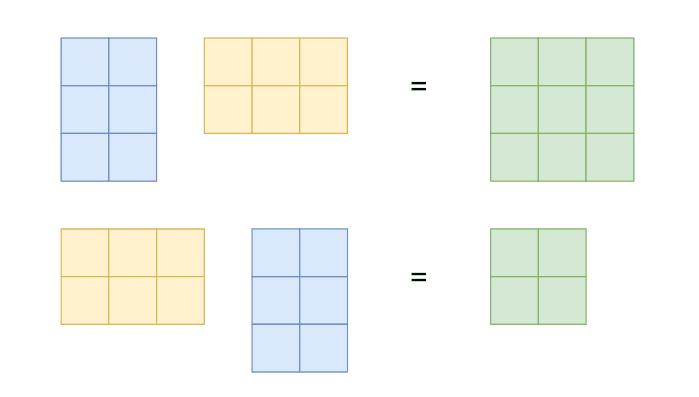
\includegraphics[width=0.92\textwidth,keepaspectratio]{docs/images/Figure2.5.png}
\caption*{\refstepcounter{figcounter}\label{fig:2-5}图~\thefigcounter 即使矩阵乘法 AB 和 BA 有意义，结果的维度也可能不同。}
\end{figure}


\textbf{定义 2.2} （单位矩阵）。 在 $ \mathbb{R}^{n \times n} $ 中，我们将 \emph{单位矩阵（identity matrix）} 定义为对角线上为 $ 1 $，其他地方为 $ 0 $ 的 $ n \times n $ 矩阵。

\begin{equation}
\begin{adjustbox}{max width=\linewidth}
\boldsymbol{I}_n :=  \begin{bmatrix} 1 & 0 & \cdots & 0 & \cdots & 0 \\ 0 & 1 & \cdots & 0 & \cdots & 0 \\ \vdots & \vdots & \ddots & \vdots & \ddots & \vdots \\ 0 & 0 & \cdots & 1 & \cdots & 0 \\ \vdots & \vdots & \ddots & \vdots & \ddots & \vdots \\ 0 & 0 & \cdots & 0 & \cdots & 1 \end{bmatrix} \in \mathbb{R}^{n \times n}
\end{adjustbox}
\tag{2.17}\label{eq:2-17}
\end{equation}

到目前我们定义了矩阵乘法、矩阵加法和单位矩阵，让我们看看矩阵的一些性质：

\begin{itemize}
\item 结合律：
\end{itemize}

\begin{equation}
\forall \boldsymbol{A} \in \mathbb{R}^{m \times n}, \ \boldsymbol{B} \in \mathbb{R}^{n \times p},\ \boldsymbol{C} \in \mathbb{R}^{p \times q} :\ (\boldsymbol{AB})\boldsymbol{C} = \boldsymbol{A} (\boldsymbol{BC})
\tag{2.18}\label{eq:2-18}
\end{equation}

\begin{itemize}
\item 交换律：
\end{itemize}

\begin{equation*}
\forall \boldsymbol {A,B} \in \mathbb{R}^{m \times n}, \ \boldsymbol {C,D} \in \mathbb{R}^{n \times p}:
\end{equation*}

\begin{equation}
(\boldsymbol{A} + \boldsymbol{B})\boldsymbol{C} = \boldsymbol{AC} + \boldsymbol{BC}
\tag{2.19a}\label{eq:2-19a}
\end{equation}

\begin{equation}
\boldsymbol{A} (\boldsymbol{C} + \boldsymbol{D}) = \boldsymbol{AC} + \boldsymbol{AD}
\tag{2.19b}\label{eq:2-19b}
\end{equation}

\begin{itemize}
\item 与单位矩阵相乘：
\end{itemize}

\begin{equation}
\forall \boldsymbol{A} \in \mathbb{R}^{m \times n}: \ \boldsymbol {I_m A} = \boldsymbol {A I_n} = \boldsymbol{A}
\tag{2.20}\label{eq:2-20}
\end{equation}

请注意，对于 $ m \not = n $，$ \boldsymbol{I}_m \not = \boldsymbol{I}_n $

\section*{2.2.2 逆和转置}
\addcontentsline{toc}{subsection}{2.2.2 逆和转置}

\textbf{定义 2.3} （逆）。对于一个方阵 $ \boldsymbol{A} \in \mathbb{R}^{n \times n} $，令矩阵 $ \boldsymbol{B} \in \mathbb{R}^{n \times n} $ 具有 $ \boldsymbol {AB} = \boldsymbol{I}_n = \boldsymbol {BA} $ 的性质。 $ \boldsymbol{B} $ 称为 $ \boldsymbol{A} $ 的 \emph{逆（inverse）} ，用 $ \boldsymbol{A}^{-1} $ 表示。

\begin{notebox}
方阵具有相同的列数和行数。
\end{notebox}

不幸的是，并非每个矩阵 $ \boldsymbol{A} $ 都具有逆 $ \boldsymbol{A}^{-1} $。 如果这个逆确实存在，则 A 称为 \emph{正则/可逆/非奇异（regular/invertible/nonsingular）} ，否则称为 \emph{奇异/不可逆（singular/noninvertible）} 。 当矩阵逆存在时，它是唯一的。 在 2.3 节中，我们将讨论通过求解线性方程组来计算矩阵逆的一般方法。

\emph{备注} （存在 2 × 2 矩阵的逆矩阵）。 考虑一个矩阵:

\begin{equation}
\boldsymbol{A} := \begin{bmatrix} a_{11} & a_{12} \\ a_{21} & a_{22} \end{bmatrix} \in \mathbb{R}^{2 \times 2}
\tag{2.21}\label{eq:2-21}
\end{equation}

如果我们将 $ \boldsymbol{A} $ 乘以

\begin{equation}
\boldsymbol{A}^{'} := \begin{bmatrix} a_{22} & -a_{12} \\ -a_{21} & a_{11} \end{bmatrix}
\tag{2.22}\label{eq:2-22}
\end{equation}

我们得到

\begin{equation}
\boldsymbol {AA^{'}} = \begin{bmatrix} a_{11}a_{22} - a_{12}a_{21} & 0 \\ 0 & a_{11}a_{22} - a_{12}a_{21} \end{bmatrix} = a_{11}a_{22} \boldsymbol{I}
\tag{2.23}\label{eq:2-23}
\end{equation}

因此

\begin{equation}
\boldsymbol{A}^{-1} =  \frac{1}{a_{11}a_{22} - a_{12}a_{21}}\begin{bmatrix} a_{22} & -a_{12} \\ -a_{21} & a_{11} \end{bmatrix}
\tag{2.24}\label{eq:2-24}
\end{equation}

当且仅当 $ a_{11}a_{22} - a_{12}a_{21} \not= 0 $。在4.1节中，我们将看到 $ a_{11}a_{22} - a_{12}a_{21} $ 是 2×2 矩阵的行列式。 此外，我们通常可以使用行列式来检查矩阵是否可逆。

\begin{notebox}
\textbf{例 2.4（逆矩阵）}
\end{notebox}

\begin{notebox}
矩阵

\begin{equation}
\begin{adjustbox}{max width=\linewidth}
\boldsymbol{A} = \begin{bmatrix} 1 & 2 & 1 \\ 4 & 4 & 5 \\ 6 & 7 & 7 \end{bmatrix}, \quad \boldsymbol{B} = \begin{bmatrix} -7 & -7 & 6 \\ 2 & 1 & -1 \\ 4 & 5 & -4 \end{bmatrix}
\end{adjustbox}
\tag{2.25}\label{eq:2-25}
\end{equation}

互为逆矩阵，因为 $ \boldsymbol {AB} = \boldsymbol{I} = \boldsymbol {BA} $。
\end{notebox}

\textbf{定义 2.4} （转置）。对于 $ \boldsymbol{A} \in \mathbb{R}^{m \times n} $，矩阵 $ \boldsymbol{B} \in \mathbb{R}^{n \times m} $ 且 $ b_{ij} = a_{ji} $ 称为 $ \boldsymbol{A} $ 的 \emph{转置（transpose）} 。 我们写 $ \boldsymbol{B} = \boldsymbol{A}^{\top} $。

一般情况下，可以通过将 $ \boldsymbol{A} $ 的列写为 $ \boldsymbol{A}^{\top} $ 的行来获得 $ \boldsymbol{A}^{\top} $ 。以下是逆和转置的重要性质：

\begin{equation}
\boldsymbol {AA^{-1}} = \boldsymbol{I} = \boldsymbol {A^{-1}A}
\tag{2.26}\label{eq:2-26}
\end{equation}

\begin{equation}
\boldsymbol {(AB)^{-1}} = \boldsymbol {B^{-1}A^{-1}}
\tag{2.27}\label{eq:2-27}
\end{equation}

\begin{equation}
\boldsymbol {(A + B)^{-1}} \not= \boldsymbol {A^{-1} + B^{-1}}
\tag{2.28}\label{eq:2-28}
\end{equation}

\begin{equation}
(\boldsymbol {A^{\top})^{\top}} = \boldsymbol{A}
\tag{2.29}\label{eq:2-29}
\end{equation}

\begin{equation}
\boldsymbol {(A + B)^{\top}} = \boldsymbol {A^{\top} + B^{\top}}
\tag{2.30}\label{eq:2-30}
\end{equation}

\begin{equation}
\boldsymbol {(AB)^{\top}} = \boldsymbol {B^{\top}A^{\top}}
\tag{2.31}\label{eq:2-31}
\end{equation}

\begin{notebox}
矩阵 $ \boldsymbol{A} $ 的主对角线是全部 $ A_{ij} $ 的集合，其中 $ i = j $。 (2.28) 的标量情况是 $ \frac{1}{2 + 4} = \frac{1}{6} \not= \frac{1}{2} + \frac{1}{6} $
\end{notebox}

\textbf{定义 2.5} （对称矩阵）。如果 $ \boldsymbol{A} = \boldsymbol{A}^{\top} $， 则矩阵 $ \boldsymbol{A} \in \mathbb{R}^{n \times n} $ 是 \emph{对称矩阵（symmetric matrix）} 。

请注意，只有 $ (n, n) $ 矩阵才可以是对称的。通常，我们称 $ (n, n) $ 矩阵也为 \emph{方阵（square matrix）} ，因为它们具有相同的行数和列数。此外，如果 $ \boldsymbol{A} $ 是可逆的，那么 $ \boldsymbol{A}^{\top} $ 也是可逆的，并且 $ (\boldsymbol{A}^{-1})^{\top} = (\boldsymbol{A}^{\top})^{-1} =: \boldsymbol{A}^{\top} $ 。

\emph{备注} （对称矩阵的和与乘积）。 对称矩阵  $ \boldsymbol {A,B} \in \mathbb{R}^{n \times n} $ 的总和总是对称的。 然而，虽然他们的乘积有意义，但它通常不是对称的：

\begin{equation}
\begin{bmatrix} 1 & 0 \\ 0 & 0 \end{bmatrix} \begin{bmatrix} 1 & 1 \\ 1 & 1 \end{bmatrix} = \begin{bmatrix} 1 & 1 \\ 0 & 0 \end{bmatrix}
\tag{2.32}\label{eq:2-32}
\end{equation}

\section*{2.2.3 乘以标量}
\addcontentsline{toc}{subsection}{2.2.3 乘以标量}

让我们看看当矩阵乘以标量 $ \lambda \in \mathbb{R} $ 时会发生什么。让 $ \boldsymbol{A} \in \mathbb{R}^{m \times n} $ 和 $ \lambda \in \mathbb{R} $，然后 $ \lambda \boldsymbol{A} =  \boldsymbol{K}, K_{ij} = \lambda a_{ij} $ 。 实际上， $ \lambda $ 缩放了 $ \boldsymbol{A} $ 的每个元素。 对于 $ \lambda,\psi \in \mathbb{R} $，以下成立：

\begin{itemize}
\item 结合律 
\end{itemize}

\begin{equation*}
(\lambda \psi)\boldsymbol{C} = \lambda(\psi \boldsymbol{C}), \ \boldsymbol{C} \in \mathbb{R}^{m \times n}
\end{equation*}

\begin{itemize}
\item 。请注意，这意味着我们可以随意移动标量值。
\end{itemize}
\begin{equation*}
\begin{adjustbox}{max width=\linewidth}
\lambda (\boldsymbol {BC}) = (\lambda \boldsymbol{B}) \boldsymbol{C} = \boldsymbol{B} (\lambda \boldsymbol{C}) = (\boldsymbol {BC}) \lambda, \ \boldsymbol{B} \in \mathbb{R}^{m \times n}, \  \boldsymbol{C} \in \mathbb{R}^{n \times k}
\end{adjustbox}
\end{equation*}
\begin{itemize}
\end{itemize}

\begin{itemize}
\item $ (\lambda \boldsymbol{C})^{\top} = \boldsymbol{C}^{\top} \lambda^{\top} = \boldsymbol{C}^{\top} \lambda = \lambda \boldsymbol{C}^{\top} $ ， 因为对于所有的 $ \lambda \in \mathbb{R}, \ \lambda = \lambda^{\top} $ 。
\end{itemize}

\begin{itemize}
\item 分配律 
\end{itemize}

\begin{equation*}
(\lambda + \psi) \boldsymbol{C} = \lambda \boldsymbol{C} + \psi \boldsymbol{C}, \ \boldsymbol{C} \in \mathbb{R}^{m \times n}
\end{equation*}

\begin{equation*}
\lambda (\boldsymbol{B} + \boldsymbol{C}) = \lambda \boldsymbol{B} + \lambda \boldsymbol{C}, \ \boldsymbol {B,C} \in \mathbb{R}^{m \times n}
\end{equation*}

\begin{notebox}
\textbf{例 2.5（分配律）}
\end{notebox}

\begin{notebox}
如果我们定义

\begin{equation}
\boldsymbol{C} := \begin{bmatrix} 1 & 2 \\ 3 & 4 \end{bmatrix}
\tag{2.33}\label{eq:2-33}
\end{equation}

那么对于任何 $ \lambda, \psi \in \mathbb{R} $，我们得到：

\begin{equation}
\begin{adjustbox}{max width=\linewidth}
(\lambda + \psi)\boldsymbol{C} = \begin{bmatrix} (\lambda + \psi)1 & (\lambda + \psi)2 \\ (\lambda + \psi)3 & (\lambda + \psi)4 \end{bmatrix} = \begin{bmatrix} \lambda + \psi & 2\lambda + 2\psi \\ 3\lambda + 3\psi & 4\lambda + 4\psi \end{bmatrix}
\end{adjustbox}
\tag{2.34a}\label{eq:2-34a}
\end{equation}

\begin{equation}
= \begin{bmatrix} \lambda & 2\lambda \\ 3\lambda & 4\lambda \end{bmatrix} + \begin{bmatrix} \psi & 2\psi \\ 3\psi & 4\psi \end{bmatrix} = \lambda \boldsymbol{C} + \psi \boldsymbol{C}
\tag{2.34b}\label{eq:2-34b}
\end{equation}
\end{notebox}

\section*{2.2.4 线性方程组的紧凑表示}
\addcontentsline{toc}{subsection}{2.2.4 线性方程组的紧凑表示}

如果我们考虑线性方程组

\begin{equation}
2x_1 + 3x_2 + 5x_3 = 1 \\
4x_1 - 2x_2 - 7x_3 = 8 \\
9x_1 + 5x_2 - 3x_3 = 2
\tag{2.35}\label{eq:2-35}
\end{equation}

并使用矩阵乘法的规则，我们可以将这个方程组写成更紧凑的形式

\begin{equation}
\begin{bmatrix} 2 & 3 & 5 \\ 4 & -2 & -7 \\ 9 & 5 & -3 \end{bmatrix} \begin{bmatrix} x_1 \\ x_2 \\ x_3 \end{bmatrix} = \begin{bmatrix} 1 \\ 8 \\ 2 \end{bmatrix}
\tag{2.36}\label{eq:2-36}
\end{equation}

请注意，$ x_1 $ 缩放第一列，$ x_2 $ 缩放第二列，$ x_3 $ 缩放第三列。

通常，线性方程组可以用其矩阵形式紧凑地表示为 $ \boldsymbol {Ax} = \boldsymbol{b} $； 见 (2.3)，乘积 $ \boldsymbol {Ax} $ 是 $ \boldsymbol{A} $ 的列的（线性）组合。 我们将在 2.5 节中更详细地讨论线性组合。

\section*{2.3 求解线性方程组}
\addcontentsline{toc}{section}{2.3 求解线性方程组}
\label{sec:2.3}

在（2.3）中，我们介绍了方程组的一般形式，即

\begin{equation}
\begin{array}{clr}
  a_{11}x_1 + \cdots + a_{1n}x_n & = b_1 \\
        & \vdots \\
  a_{m1}x_1 +  \cdots + a_{mn}x_n & = b_m
\end{array}
\tag{2.37}\label{eq:2-37}
\end{equation}

其中 $ a_{ij} \in \mathbb{R} $ 和 $ b_i \in \mathbb{R} $ 是已知常数， $ x_j $ 是未知数， $ i = 1,...,m, \ j = 1,...,n $。到目前为止，我们看到矩阵可以用来精确表达线性方程组的紧凑形式，以便我们可以写出 $ \boldsymbol {Ax} = \boldsymbol{b} $ ，参见（2.10）。 此外，我们定义了基本的矩阵运算，例如矩阵的加法和乘法。 在下文中，我们将专注于求解线性方程组并提供一种求矩阵逆的算法。

\section*{2.3.1 特解和通解}
\addcontentsline{toc}{subsection}{2.3.1 特解和通解}

在讨论如何对线性方程组进行一般求解之前，让我们先看一个例子。 考虑方程组

\begin{equation}
\begin{bmatrix} 1 & 0 & 8 & -4 \\ 0 & 1 & 2 & 12 \end{bmatrix} \begin{bmatrix} x_1 \\ x_2 \\ x_3 \\ x_4 \end{bmatrix} = \begin{bmatrix} 42 \\ 8 \end{bmatrix}
\tag{2.38}\label{eq:2-38}
\end{equation}

该系统有两个方程和四个未知数。 因此，通常我们会期望有无穷多个解。 这个方程组的形式特别简单，其中前两列由 $ 1 $ 和 $ 0 $ 组成。请记住，我们要找到标量 $ x_1,...,x_4 $ ，使得 $ \sum^{4}_{i=1}{x_i \boldsymbol{c}_i} = \boldsymbol{b} $，其中我们将 $ \boldsymbol{c}_i $ 定义为矩阵的第 $ i $ 列，将 $ \boldsymbol{b} $ 定义为(2.38)的右侧。我们对第一列乘42，第二列乘8，便可以立即找到 (2.38) 中问题的解

\begin{equation}
\boldsymbol{b} = \begin{bmatrix} 42 \\ 8 \end{bmatrix} = 42 \begin{bmatrix} 1 \\ 0 \end{bmatrix} + 8 \begin{bmatrix} 0 \\ 1 \end{bmatrix}
\tag{2.39}\label{eq:2-39}
\end{equation}

因此，一个解是 $ [42,8,0,0]^{\top} $ 。 这种解称为 \emph{特解（particular solution/special solution）} 。然而，这并不是这个线性方程组的唯一解。 为了捕获所有其他解，我们需要创造性地使用矩阵的列以一种有意义的方式生成 $ \boldsymbol{0} $：将 $ \boldsymbol{0} $ 添加到我们的特解中并不会改变特解。 为此，我们使用前两列（这种非常简单的形式）表示第三列

\begin{equation}
\begin{bmatrix} 8 \\ 2 \end{bmatrix} = 8 \begin{bmatrix} 1 \\ 0 \end{bmatrix} + 2 \begin{bmatrix} 0 \\ 1 \end{bmatrix}
\tag{2.40}\label{eq:2-40}
\end{equation}

所以 $ \boldsymbol{0} = 8 \boldsymbol{c}_1 + 2 \boldsymbol{c}_2 - 1 \boldsymbol{c}_3 + 0 \boldsymbol{c}_4 $ 且 $ (x_1,x_2,x_3,x_4) = (8,2,-1,0) $。事实上，这个解的任何 $ \lambda{_1} \in \mathbb{R} $ 缩放都会产生 $ \boldsymbol{0} $ 向量，即，

\begin{equation}
\begin{adjustbox}{max width=\linewidth}
\begin{bmatrix} 1 & 0 & 8 & -4 \\ 0 & 1 & 2 & 12 \end{bmatrix} \left( \lambda{_1}   \begin{bmatrix} 8 \\ 2 \\ -1 \\ 0 \end{bmatrix} \right) = \lambda{_1} (8 \boldsymbol{c}_1 + 2 \boldsymbol{c}_2 - \boldsymbol{c}_3) = \boldsymbol{0}
\end{adjustbox}
\tag{2.41}\label{eq:2-41}
\end{equation}

按照相同的推理思路，我们使用前两列表达（2.38）中矩阵的第四列，并为任何 $ \lambda{_3} \in \mathbb{R} $ 生成另一组有意义的 $ \boldsymbol{0} $

\begin{equation}
\begin{adjustbox}{max width=\linewidth}
\begin{bmatrix} 1 & 0 & 8 & -4 \\ 0 & 1 & 2 & 12 \end{bmatrix} \left( \lambda{_2}   \begin{bmatrix} -4 \\ 12 \\ 0 \\ -1 \end{bmatrix} \right) = \lambda{_3} (-4 \boldsymbol{c}_1 + 12 \boldsymbol{c}_2 - \boldsymbol{c}_4) = \boldsymbol{0}
\end{adjustbox}
\tag{2.42}\label{eq:2-42}
\end{equation}

综上所述，我们得到式~\eqref{eq:2-38}中方程组的所有解，称为 \emph{通解（general solution）} ，集合为

\begin{equation}
\begin{adjustbox}{max width=\linewidth}
\left\{ \boldsymbol{x} \in \mathbb{R}^4 : \boldsymbol{x} =  \begin{bmatrix} 42 \\ 8 \\ 0 \\ 0 \end{bmatrix} + \lambda{_1} \begin{bmatrix} 8 \\ 2 \\ -1 \\ 0 \end{bmatrix} + \lambda{_2} \begin{bmatrix} -4 \\ 12 \\ 0 \\ -1 \end{bmatrix}, \  \lambda{_1},\lambda{_2} \in \mathbb{R} \right\}
\end{adjustbox}
\tag{2.43}\label{eq:2-43}
\end{equation}

\emph{备注} 。 我们遵循的一般方法包括以下三个步骤：

\begin{enumerate}
\item 求 $ \boldsymbol {Ax} = \boldsymbol{b} $ 的特解。
\item 求 $ \boldsymbol {Ax} = \boldsymbol{0} $ 的所有解。
\item 结合步骤1和2的解决方案成为通解。
\end{enumerate}

通解和特解都不是唯一的。

前面例子中的线性方程组很容易求解，因为（2.38）中的矩阵具有这种特别方便的形式，这使我们可以通过检查找到特解和通解。 然而，一般方程系统不是这种简单的形式。 幸运的是，存在一种将任何线性方程组转换为这种特别简单的形式的构造算法：高斯消元法（Gaussian elimination）。 高斯消元的关键是线性方程组的初等变换，将方程组转化为简单的形式。 然后，我们可以将这三个步骤应用到这种简单形式上，正是我们刚刚在 (2.38) 示例上下文中讨论的方法。

\section*{2.3.2 初等变换}
\addcontentsline{toc}{subsection}{2.3.2 初等变换}

求解线性方程组的关键是保持解集不变的 \emph{初等变换（elementary transformations）} ，同时将方程组转换为更简单的形式：

\begin{itemize}
\item 交换两个方程（矩阵中的行代表方程组）
\item 方程（行）乘以一个常数 $ \lambda \in \mathbb{R} \backslash \{0\} $ 
\item 两个方程相加（行）
\end{itemize}

\begin{notebox}
\textbf{例 2.6}
\end{notebox}

\begin{notebox}
对于 $ a \in \mathbb{R} $，我们寻求以下方程组的所有解：

\begin{equation}
\begin{adjustbox}{max width=\linewidth}
\begin{array}{clr}
  -2x_1 & + & 4x_2 & - & 2x_3 & - & x_4 & + & 4x_5 & = & -3 \\
  4x_1 & - & 8x_2 & + & 3x_3 & - & 3x_4 & + & x_5 & = & 2 \\ 
  x_1 & - & 2x_2 & + & x_3 & - & x_4 & + & x_5 & = & 0 \\ 
  x_1 & - & 2x_2 & & & - & 3x_4 & + & 4x_5 & = & a
\end{array}
\end{adjustbox}
\tag{2.44}\label{eq:2-44}
\end{equation}

我们首先将这个方程组转换为紧凑矩阵形式 $ \boldsymbol {Ax} = \boldsymbol{b} $。我们不再明确提及变量 $ \boldsymbol{x} $ 并构建 \emph{增广矩阵（augmented matrix）} （形式为 $ [\boldsymbol{A} \mid \boldsymbol{b}] $）：

\begin{equation*}
\begin{adjustbox}{max width=\linewidth}
\left[ \begin{array}{ccccc|c}
    -2 & 4 & -2 & -1 & 4 & -3 \\ 
    4 & -8 & 3 & -3 & 1 & 2 \\
    1 & -2 & 1 & -1 & 1 & 0 \\
    1 & -2 & 0 & -3 & 4 & a 
\end{array} \right]
\end{adjustbox}
\end{equation*}

在 (2.44) 中，我们使用垂直线将左侧和右侧分开。我们用 $ \leadsto $ 来表示增广矩阵的初等变换。 交换第 1 行和第 3 行，结果为：

\begin{equation*}
\begin{adjustbox}{max width=\linewidth}
\left[ \begin{array}{ccccc|c}
    1 & -2 & 1 & -1 & 1 & 0 \\ 
    4 & -8 & 3 & -3 & 1 & 2 \\
    -2 & 4 & -2 & -1 & 4 & -3 \\
    1 & -2 & 0 & -3 & 4 & a 
\end{array} \right]
\end{adjustbox}
\end{equation*}

当我们应用指定的初等变换时（例如从第 2 行减去 4 倍的第 1 行），得到：

\begin{equation*}
\begin{adjustbox}{max width=\linewidth}
\left[ \begin{array}{ccccc|c}
    1 & -2 & 1 & -1 & 1 & 0 \\ 
    0 & 0 & -1 & 1 & -3 & 2 \\
    0 & 0 & 0 & -3 & 6 & -3 \\
    0 & 0 & -1 & -2 & 3 & a 
\end{array} \right]
\end{adjustbox}
\end{equation*}

进而通过消元得到：

\begin{equation*}
\begin{adjustbox}{max width=\linewidth}
\leadsto \left[ \begin{array}{ccccc|c}
    1 & -2 & 1 & -1 & 1 & 0 \\ 
    0 & 0 & -1 & 1 & -3 & 2 \\
    0 & 0 & 0 & -3 & 6 & -3 \\
    0 & 0 & 0 & 0 & 0 & a + 1 
\end{array} \right]
\end{adjustbox}
\end{equation*}

将第 2 行乘 $ -1 $，第 3 行乘 $ -\frac{1}{3} $，得到：

\begin{equation*}
\begin{adjustbox}{max width=\linewidth}
\leadsto \left[ \begin{array}{ccccc|c}
    1 & -2 & 1 & -1 & 1 & 0 \\ 
    0 & 0 & 1 & -1 & 3 & -2 \\
    0 & 0 & 0 & 1 & -2 & 1 \\
    0 & 0 & 0 & 0 & 0 & a + 1 
\end{array} \right]
\end{adjustbox}
\end{equation*}

这个（增广）矩阵呈现出一种非常便利的形式，即 \emph{行阶梯形矩阵（REF, row-echelon form）} 。将这个紧凑表示还原为包含待求变量的显式表示，我们得到：

\begin{equation}
\begin{adjustbox}{max width=\linewidth}
\begin{array}{clr}
  x_1 & - & 2x_2 & + & x_3 & - & x_4 & + & x_5 & = & 0 \\
  & & & & x_3 & - & x_4 & + & 3x_5 & = & -2 \\ 
  & & & & & & x_4 & - & 2x_5 & = & 1 \\ 
  & & & & & & & & 0 & = & a + 1
\end{array}
\end{adjustbox}
\tag{2.45}\label{eq:2-45}
\end{equation}

只有当 $ a = -1 $ 时，才能解出这个方程组。其 \emph{特解（particular solution）} 是：

\begin{equation}
\begin{bmatrix} x_1 \\ x_2 \\ x_3 \\ x_4 \\ x_5 \end{bmatrix} = \begin{bmatrix} 2 \\ 0 \\ -1 \\ 1 \\ 0 \end{bmatrix}
\tag{2.46}\label{eq:2-46}
\end{equation}

其 \emph{通解（general solution）} ，也就是所有可能解的集合，是：

\begin{equation}
\begin{adjustbox}{max width=\linewidth}
\left\{ \boldsymbol{x} \in \mathbb{R}^5: \boldsymbol{x} = \begin{bmatrix} 2 \\ 0 \\ -1 \\ 1 \\ 0 \end{bmatrix} + \lambda_{1}\begin{bmatrix} 2 \\ 1 \\ 0 \\ 0 \\ 0 \end{bmatrix} + \lambda_{2}\begin{bmatrix} 2 \\ 0 \\ -1 \\ 2 \\ 1 \end{bmatrix}, \ \lambda_{1}, \lambda_{2} \in \mathbb{R} \right\}
\end{adjustbox}
\tag{2.47}\label{eq:2-47}
\end{equation}
\end{notebox}

下面，我们将详细介绍一种构造方法来获得线性方程组的特解和通解。

\emph{备注} （主元和阶梯结构）。 行的首项系数（leading coefficient，从左侧开始的第一个非零数）称为 \emph{主元（pivot）} ，并且始终严格位于其上一行的主元的右侧。 因此，任何行阶梯形式的方程组都具有“阶梯”结构。

\textbf{定义2.6}（行阶梯形矩阵）。 一个矩阵是行阶梯形矩阵，如果满足：

\begin{itemize}
\item 所有只包含0的行都在矩阵的底部；相应地，所有包含至少一个非零元素的行都位于只包含零的行之上。
\end{itemize}

\begin{itemize}
\item 只看非零行，从左起的第一个非零数（也称为 \emph{主元（pivot）} 或 \emph{领先系数（leading coefficient）} ）总是严格地在它上面一行的主元的右边。
\end{itemize}

\begin{notebox}
在其他文档资料中，有时需要主元为1。
\end{notebox}

\emph{备注} （基本变量和自由变量）。 行阶梯形的主元对应的变量称为 \emph{基本变量（basic variables）} ，其他变量为 \emph{自由变量（free variables）} 。 例如，在（2.45）中，$ x_1, x_3, x_4 $ 是基本变量，而 $ x_2, x_5 $ 是自由变量。

\emph{备注} （求特解）。行阶梯形使我们在求特解时变得更容易。为了做到这一点，我们用主元列表示方程组的右边列，使得 $ \boldsymbol{b} = \sum_{i=1}^{P}{{\lambda}_i \boldsymbol{p}_i}, i = 1,...,P $， 其中 $ \boldsymbol{p}_i $ 为主元列。如果我们从最右边的主元列开始并向左计算，则很容易确定 $ {\lambda}_i $ 。

在前面的例子中，我们会尝试找到 $ {\lambda}_1, {\lambda}_2, {\lambda}_3 $ 以便

\begin{equation}
\begin{adjustbox}{max width=\linewidth}
{\lambda}_1\begin{bmatrix} 1 \\ 0 \\ 0 \\ 0 \end{bmatrix} + {\lambda}_2\begin{bmatrix} 1 \\ 1 \\ 0 \\ 0 \end{bmatrix} + {\lambda}_3\begin{bmatrix} -1 \\ -1 \\ 1 \\ 0 \end{bmatrix} = \begin{bmatrix} 0 \\ -2 \\ 1 \\ 0 \end{bmatrix}
\end{adjustbox}
\tag{2.48}\label{eq:2-48}
\end{equation}

从这里，我们相对直接地发现 $ {\lambda}_3 = 1, {\lambda}_2 = -1, {\lambda}_1 = 2 $。当我们把所有东西放在一起时，我们一定不要忘记我们将系数隐式设置为0的非主元列。因此，我们得到特解 $ x = [2, 0, −1, 1, 0]^{\top} $。

\emph{备注} （简化行阶梯形）如果一个方程组是简化行阶梯形（也叫做行简化阶梯形或行正则形）：

\begin{itemize}
\item 它采用行梯队形式。
\item 每个主元都是 1。
\item 主元是其列中唯一的非零元素。
\end{itemize}

简化行阶梯形将在2.3.3节后面发挥重要作用，因为它允许我们以一种直接的方式确定线性方程组的通解。

\emph{备注} （高斯消元法）。 \emph{高斯消元（Gaussian Elimination）} 是一种算法，可以通过执行初等变换将线性方程组变为简化行阶梯形。

\begin{notebox}
\textbf{例2.7（简化行阶梯形）} 验证以下矩阵是否采用简化行阶梯形（主元以\textbf{粗体}显示）：

\begin{equation}
\begin{adjustbox}{max width=\linewidth}
\boldsymbol{A} = \begin{bmatrix} \boldsymbol{1} & 3 & 0 & 0 & 3\\ 0 & 0 & \boldsymbol{1} & 0 & 9 \\ 0 & 0 & 0 & \boldsymbol{1} & -4 \end{bmatrix}
\end{adjustbox}
\tag{2.49}\label{eq:2-49}
\end{equation}

求 $ \boldsymbol {Ax = 0} $ 的解的关键是查看非主元列，我们需要将其表示为主元列的（线性）组合。简化行阶梯形使得这相对简单一些，我们根据其左侧的主元列的总和和倍数来表示非主元列：第二列是第一列的 3 倍（我们可以忽略第二列的右侧的主元列）。因此，为了得到 $ \boldsymbol{0} $ ，我们需要从第一列的三倍中减去第二列。 现在，我们看第五列，这是我们的第二个非主元列。 第五列可以表示为第一个主元列的 3 倍、第二个主元列的 9 倍和第三个主元列的 -4 倍。 我们需要跟踪主元列的索引并将其转换为第一列的 3 倍，第二列（非主元列）的 0 倍，第三列（我们的第二个主元列）的 9 倍 ，第四列的 -4 倍（即第三个主元列）。 然后我们需要减去第五列得到 $ \boldsymbol{0} $ 。最终，我们仍然在求解一个齐次方程组。 总而言之，$ \boldsymbol {Ax = 0}, \boldsymbol{x} \in \mathbb{R}^5 $ 的所有解由下式给出 \textbackslash\{\}left\textbackslash\{\}\{ \textbackslash\{\}boldsymbol\{x\} \textbackslash\{\}in \textbackslash\{\}mathbb\{R\}\textasciicircum{}5: \textbackslash\{\}boldsymbol\{x\} = \textbackslash\{\}lambda\{\emph{1}\begin{bmatrix} 3 \\ -1 \\ 0 \\ 0 \\ 0 \end{bmatrix} + \lambda}\{2\}\textbackslash\{\}begin\{bmatrix\} 3 \textbackslash\{\}\textbackslash\{\} 0 \textbackslash\{\}\textbackslash\{\} 9 \textbackslash\{\}\textbackslash\{\} -4 \textbackslash\{\}\textbackslash\{\} -1 \textbackslash\{\}end\{bmatrix\}, \textbackslash\{\} \textbackslash\{\}lambda\_\{1\}, \textbackslash\{\}lambda\_\{2\} \textbackslash\{\}in \textbackslash\{\}mathbb\{R\} \textbackslash\{\}right\textbackslash\{\}\} \textbackslash\{\}tag\{2.50\}
\end{notebox}

\section*{2.3.3 减1技巧}
\addcontentsline{toc}{subsection}{2.3.3 减1技巧}

下面，我们介绍一个实用的技巧，来直接读出齐次线性方程组 $ \boldsymbol {Ax} = \boldsymbol{0} $ 的解 $ \boldsymbol{x} $，其中 $ \boldsymbol{A} \in \mathbb{R}^{k \times n} $，$ \boldsymbol{x} \in \mathbb{R}^n $。

首先，我们假设 $ \boldsymbol{A} $ 已经化为简化行阶梯形（reduced row-echelon form），且不包含全零行，即：

\begin{equation}
\begin{adjustbox}{max width=\linewidth}
\boldsymbol{A} = \begin{bmatrix}
0 & \cdots & 0 & \boldsymbol{1} & * & \cdots & * & 0 & * & \cdots & * & 0 & * & \cdots & * \\
\vdots & & \vdots & 0 & 0 & \cdots & 0 & \boldsymbol{1} & * & \cdots & * & \vdots & \vdots & & \vdots \\
\vdots & & \vdots & \vdots & \vdots & & \vdots & 0 & \cdots & \cdots & 0 & \vdots & \vdots & & \vdots \\
\vdots & & \vdots & \vdots & \vdots & & \vdots & \vdots & & & \vdots & \vdots & \vdots & & \vdots \\
0 & \cdots & 0 & 0 & 0 & \cdots & 0 & 0 & \cdots & \cdots & 0 & \boldsymbol{1} & * & \cdots & *
\end{bmatrix}
\end{adjustbox}
\tag{2.51}\label{eq:2-51}
\end{equation}

其中 $ * $ 可以是任意实数，其约束条件是：每行的第一个非零元素必须为 1，且该主元所在列的所有其他元素都必须为 0。含有主元（以\textbf{粗体}标出）的列 $ j_1, \ldots, j_k $ 是标准单位向量 $ \boldsymbol{e}_1, \ldots, \boldsymbol{e}_k \in \mathbb{R}^k $。我们通过添加 $ n - k $ 行形如下式的行，将该矩阵扩展为一个 $ n \times n $ 矩阵 $ \tilde{\boldsymbol{A}} $：

\begin{equation}
\begin{bmatrix} 0 & \cdots & 0 & -1 & 0 & \cdots & 0 \end{bmatrix}
\tag{2.52}\label{eq:2-52}
\end{equation}

从而使增广矩阵 $ \tilde{\boldsymbol{A}} $ 的对角线元素仅包含 1 或 -1。此时，增广矩阵 $ \tilde{\boldsymbol{A}} $ 中对角线上包含 -1 的列，就是齐次方程组 $ \boldsymbol {Ax} = \boldsymbol{0} $ 的解。更确切地说，这些列构成了 $ \boldsymbol {Ax} = \boldsymbol{0} $ 解空间的一组基（第 2.6.1 节），我们稍后将其称为 \emph{核（kernel）} 或 \emph{零空间（null space）} （参见第 2.7.3 节）。

\begin{notebox}
\textbf{例 2.8（减1技巧）}
\end{notebox}

\begin{notebox}
让我们重新审视 (2.49) 中的矩阵，它已经是简化行阶梯形：

\begin{equation}
\begin{adjustbox}{max width=\linewidth}
\boldsymbol{A} = \begin{bmatrix} \boldsymbol{1} & 3 & 0 & 0 & 3 \\ 0 & 0 & \boldsymbol{1} & 0 & 9 \\ 0 & 0 & 0 & \boldsymbol{1} & -4 \end{bmatrix}
\end{adjustbox}
\tag{2.53}\label{eq:2-53}
\end{equation}

现在我们在对角线上缺少主元的位置添加形如 (2.52) 的行，将该矩阵扩展为一个 $ 5 \times 5 $ 的矩阵，得到：

\begin{equation}
\begin{adjustbox}{max width=\linewidth}
\tilde{\boldsymbol{A}} = \begin{bmatrix} \boldsymbol{1} & 3 & 0 & 0 & 3 \\ 0 & \boldsymbol{-1} & 0 & 0 & 0 \\ 0 & 0 & \boldsymbol{1} & 0 & 9 \\ 0 & 0 & 0 & \boldsymbol{1} & -4 \\ 0 & 0 & 0 & 0 & \boldsymbol{-1} \end{bmatrix}
\end{adjustbox}
\tag{2.54}\label{eq:2-54}
\end{equation}

从这种形式中，我们可以立即通过选取 $ \tilde{\boldsymbol{A}} $ 中对角线上包含 -1 的列，读出 $ \boldsymbol {Ax} = \boldsymbol{0} $ 的解：

\begin{equation}
\begin{adjustbox}{max width=\linewidth}
\left\{ \boldsymbol{x} \in \mathbb{R}^5 : \boldsymbol{x} = \lambda_1 \begin{bmatrix} 3 \\ -1 \\ 0 \\ 0 \\ 0 \end{bmatrix} + \lambda_2 \begin{bmatrix} 3 \\ 0 \\ 9 \\ -4 \\ -1 \end{bmatrix}, \ \lambda_1, \lambda_2 \in \mathbb{R} \right\}
\end{adjustbox}
\tag{2.55}\label{eq:2-55}
\end{equation}

这与我们在 (2.50) 中通过“直接观察”得到的解完全相同。
\end{notebox}

\subsection*{求逆矩阵（Calculating the Inverse）}
\addcontentsline{toc}{subsubsection}{求逆矩阵（Calculating the Inverse）}

为了计算矩阵 $ \boldsymbol{A} \in \mathbb{R}^{n \times n} $ 的逆矩阵 $ \boldsymbol{A}^{-1} $，我们需要找到一个满足 $ \boldsymbol{A} \boldsymbol{X} = \boldsymbol{I}_n $ 的矩阵 $ \boldsymbol{X} $。此时即有 $ \boldsymbol{X} = \boldsymbol{A}^{-1} $。我们可以将其写为一组联立的线性方程组 $ \boldsymbol{A} \boldsymbol{X} = \boldsymbol{I}_n $，其中求解未知矩阵 $ \boldsymbol{X} = [\boldsymbol{x}_1 \mid \cdots \mid \boldsymbol{x}_n] $。我们使用增广矩阵记号来紧凑地表示这组线性方程组，并得到：

\begin{equation}
[\boldsymbol{A} \mid \boldsymbol{I}_n] \leadsto \cdots \leadsto [\boldsymbol{I}_n \mid \boldsymbol{A}^{-1}]
\tag{2.56}\label{eq:2-56}
\end{equation}

这意味着，如果我们将增广方程组化为简化行阶梯形，就可以直接在方程组的右半部分读出逆矩阵。因此，确定矩阵的逆等价于求解线性方程组。

\begin{notebox}
\textbf{例 2.9（利用高斯消元法计算逆矩阵）}
\end{notebox}

\begin{notebox}
为了求矩阵

\begin{equation}
\begin{adjustbox}{max width=\linewidth}
\boldsymbol{A} = \begin{bmatrix} 1 & 0 & 2 & 0 \\ 1 & 1 & 0 & 0 \\ 1 & 2 & 0 & 1 \\ 1 & 1 & 1 & 1 \end{bmatrix}
\end{adjustbox}
\tag{2.57}\label{eq:2-57}
\end{equation}

的逆矩阵，我们写出增广矩阵：

\begin{equation*}
\begin{adjustbox}{max width=\linewidth}
[\boldsymbol{A} \mid \boldsymbol{I}_4] = \left[ \begin{array}{cccc|cccc} 1 & 0 & 2 & 0 & 1 & 0 & 0 & 0 \\ 1 & 1 & 0 & 0 & 0 & 1 & 0 & 0 \\ 1 & 2 & 0 & 1 & 0 & 0 & 1 & 0 \\ 1 & 1 & 1 & 1 & 0 & 0 & 0 & 1 \end{array} \right]
\end{adjustbox}
\end{equation*}

并使用高斯消元法将其化为简化行阶梯形：

\begin{equation*}
\begin{adjustbox}{max width=\linewidth}
\left[ \begin{array}{cccc|cccc} 1 & 0 & 0 & 0 & -1 & 2 & -2 & 2 \\ 0 & 1 & 0 & 0 & 1 & -1 & 2 & -2 \\ 0 & 0 & 1 & 0 & 1 & -1 & 1 & -1 \\ 0 & 0 & 0 & 1 & -1 & 0 & -1 & 2 \end{array} \right]
\end{adjustbox}
\end{equation*}

从而所求的逆矩阵即为其右半部分：

\begin{equation}
\begin{adjustbox}{max width=\linewidth}
\boldsymbol{A}^{-1} = \begin{bmatrix} -1 & 2 & -2 & 2 \\ 1 & -1 & 2 & -2 \\ 1 & -1 & 1 & -1 \\ -1 & 0 & -1 & 2 \end{bmatrix}
\end{adjustbox}
\tag{2.58}\label{eq:2-58}
\end{equation}

我们可以通过计算矩阵乘法 $ \boldsymbol{A} \boldsymbol{A}^{-1} $ 并观察是否恢复为 $ \boldsymbol{I}_4 $，来验证 (2.58) 确实是所求的逆矩阵。
\end{notebox}

\medskip\hrule\medskip

\section*{2.3.4 求解线性方程组的算法}
\addcontentsline{toc}{subsection}{2.3.4 求解线性方程组的算法}

下面，我们简要讨论求解形如 $ \boldsymbol {Ax} = \boldsymbol{b} $ 的线性方程组的方法。我们在此假设解是存在的。若无解，则需要求助于近似解，这不在本章的讨论范围内。求解近似问题的一种方法是使用线性回归方法，我们将在第 9 章中进行详细讨论。

在特殊情况下，我们或许能够求出逆矩阵 $ \boldsymbol{A}^{-1} $，从而使 $ \boldsymbol {Ax} = \boldsymbol{b} $ 的解直接表示为 $ \boldsymbol{x} = \boldsymbol{A}^{-1} \boldsymbol{b} $。然而，这仅在 $ \boldsymbol{A} $ 是方阵且可逆时才可行，而实际情况往往并非如此。否则，在较为温和的假设下（即 $ \boldsymbol{A} $ 具有列线性无关），我们可以使用以下变换：

\begin{equation}
\boldsymbol {Ax} = \boldsymbol{b} \iff \boldsymbol{A}^\top \boldsymbol {Ax} = \boldsymbol{A}^\top \boldsymbol{b} \iff \boldsymbol{x} = (\boldsymbol{A}^\top \boldsymbol{A})^{-1} \boldsymbol{A}^\top \boldsymbol{b}
\tag{2.59}\label{eq:2-59}
\end{equation}

并利用 \emph{Moore-Penrose 伪逆（Moore-Penrose pseudo-inverse）} $ (\boldsymbol{A}^\top \boldsymbol{A})^{-1} \boldsymbol{A}^\top $ 来确定求解 $ \boldsymbol {Ax} = \boldsymbol{b} $ 的解 (2.59)，该解也对应于最小范数最小二乘解。这种方法的缺点在于，计算矩阵与矩阵相乘以及计算 $ \boldsymbol{A}^\top \boldsymbol{A} $ 的逆需要大量的计算开销。此外，出于数值精度的考虑，通常不推荐直接计算逆矩阵或伪逆。

因此，在下文中我们将简要讨论求解线性方程组的替代方法。

高斯消元法在计算行列式（第 4.1 节）、检验一组向量是否线性无关（第 2.5 节）、计算矩阵的逆（第 2.2.2 节）、计算矩阵的秩（第 2.6.2 节）以及确定向量空间的基（第 2.6.1 节）中起着重要作用。高斯消元法是求解包含成千上万个变量的线性方程组的一种直观且构造性的方法。然而，对于具有数百万个变量的系统，高斯消元法在实际中是不可行的，因为所需的算术运算次数随联立方程的数量呈三次阶（$ O(n^3) $）增长。

在实际应用中，大规模线性方程组通常采用间接方法求解：要么使用定常迭代法（stationary iterative methods），例如理查森迭代法（Richardson method）、雅可比迭代法（Jacobi method）、高斯-赛德尔迭代法（Gauß-Seidel method）和逐次超松弛法（successive over-relaxation method, SOR）；要么使用克雷洛夫子空间法（Krylov subspace methods），例如共轭梯度法（conjugate gradients, CG）、广义极小残差法（generalized minimal residual, GMRES）或双共轭梯度法（biconjugate gradients, BiCG）。更多细节可参考 Stoer 和 Burlirsch（2002）、Strang（2003）以及 Liesen 和 Mehrmann（2015）的著作。

设 $ \boldsymbol{x}^* $ 为 $ \boldsymbol {Ax} = \boldsymbol{b} $ 的一个解。这些迭代方法的核心思想是构建形如下式的迭代格式：

\begin{equation}
\boldsymbol{x}^{(k+1)} = \boldsymbol{C} \boldsymbol{x}^{(k)} + \boldsymbol{d}
\tag{2.60}\label{eq:2-60}
\end{equation}

其中选取合适的 $ \boldsymbol{C} $ 和 $ \boldsymbol{d} $，使得残差误差 $ \| \boldsymbol{x}^{(k+1)} - \boldsymbol{x}^* \| $ 在每次迭代中逐渐减小并收敛到 $ \boldsymbol{x}^* $。我们将在第 3.1 节中介绍范数 $ \| \cdot \| $，它使我们能够度量向量之间的相似度。

\section*{2.4 向量空间}
\addcontentsline{toc}{section}{2.4 向量空间}
\label{sec:2.4}

到目前为止，我们已经探讨了线性方程组及其求解方法（第 2.3 节）。我们看到线性方程组可以使用矩阵-向量记号进行紧凑的表示 (2.10)。在下文中，我们将更深入地探讨 \emph{向量空间（vector spaces）} ，即向量所处的一种结构化空间。

在本章开头，我们非正式地将向量描述为可以相加并且可以与标量相乘的对象，而且运算后它们仍然保持为相同类型的对象。现在，我们准备将这一概念形式化。我们首先介绍 \emph{群（group）} 的概念，群是一个包含若干元素的集合以及定义在这些元素上的运算，该运算保留了集合的某种结构。

\section*{2.4.1 群}
\addcontentsline{toc}{subsection}{2.4.1 群}

群在计算机科学中扮演着重要角色。除了为集合上的运算提供基础框架之外，群还广泛应用于密码学、编码理论和计算机图形学中。

\textbf{定义 2.7}（群）。考虑一个集合 $ G $ 以及定义在 $ G $ 上的运算 $ \otimes: G \times G \to G $。如果满足以下条件，则 $ G := (G, \otimes) $ 称为一个 \emph{群（group）} ：

\begin{enumerate}
\item $ G $ 在 $ \otimes $ 下的 \emph{闭包（closure）} 性：$ \forall x, y \in G : x \otimes y \in G $
\item \emph{结合律（associativity）} ：$ \forall x, y, z \in G : (x \otimes y) \otimes z = x \otimes (y \otimes z) $
\item \emph{单位元（neutral element）} ：$ \exists e \in G \ \forall x \in G : x \otimes e = x $ 且 $ e \otimes x = x $
\item \emph{逆元（inverse element）} ：$ \forall x \in G \ \exists y \in G : x \otimes y = e $ 且 $ y \otimes x = e $。我们通常记 $ x^{-1} $ 为 $ x $ 的逆元。
\end{enumerate}

\emph{备注} 。逆元是相对于运算 $ \otimes $ 定义的，并不必然意味着 $ \frac{1}{x} $。

如果还满足 $ \forall x, y \in G : x \otimes y = y \otimes x $，则 $ G = (G, \otimes) $ 称为一个 \emph{阿贝尔群（Abelian group）} （交换群）。

\begin{notebox}
\textbf{例 2.10（群）}
\end{notebox}

\begin{notebox}
让我们看一些集合及其关联运算的例子，检验它们是否构成群：

\begin{itemize}
\item $ (\mathbb{Z}, +) $ 是一个群。
\item $ (\mathbb{N}_0, +) $ 不是群（其中 $ \mathbb{N}_0 := \mathbb{N} \cup \{0\} $）：尽管 $ (\mathbb{N}_0, +) $ 拥有单位元（$ 0 $），但缺少逆元。
\item $ (\mathbb{Z}, \cdot) $ 不是群：尽管 $ (\mathbb{Z}, \cdot) $ 包含单位元（$ 1 $），但对于任意 $ z \in \mathbb{Z}, z \neq \pm 1 $，都缺少逆元。
\item $ (\mathbb{R}, \cdot) $ 不是群，因为 $ 0 $ 没有逆元。
\item $ (\mathbb{R} \setminus \{0\}, \cdot) $ 是一个阿贝尔群。
\item 若加法按分量定义，即： 则对于 $ n \in \mathbb{N} $，$ (\mathbb{R}^n, +) $ 和 $ (\mathbb{Z}^n, +) $ 均为阿贝尔群。此时，逆元为 $ (x_1, \ldots, x_n)^{-1} := (-x_1, \ldots, -x_n) $，单位元为 $ \boldsymbol{e} = (0, \ldots, 0) $。
\end{itemize}
\begin{equation}
(x_1, \ldots, x_n) + (y_1, \ldots, y_n) = (x_1 + y_1, \ldots, x_n + y_n)
\tag{2.61}\label{eq:2-61}
\end{equation}
\begin{itemize}
\item $ (\mathbb{R}^{m \times n}, +) $（$ m \times n $ 矩阵的集合）是一个阿贝尔群（采用 (2.61) 定义的按元素加法）。
\end{itemize}
\end{notebox}

\begin{notebox}
让我们仔细考察 $ (\mathbb{R}^{n \times n}, \cdot) $，即采用 (2.13) 所定义的矩阵乘法的 $ n \times n $ 矩阵集合：

\begin{itemize}
\item 封闭性和结合律直接由矩阵乘法的定义得出。
\item 单位元：单位矩阵 $ \boldsymbol{I}_n $ 是 $ (\mathbb{R}^{n \times n}, \cdot) $ 中关于矩阵乘法“$ \cdot $”的单位元。
\item 逆元：如果逆矩阵存在（即 $ \boldsymbol{A} $ 为正则/可逆矩阵），则 $ \boldsymbol{A}^{-1} $ 为 $ \boldsymbol{A} \in \mathbb{R}^{n \times n} $ 的逆元；且恰好在这种情况下，$ (\mathbb{R}^{n \times n}, \cdot) $ 构成一个群，称为一般线性群。
\end{itemize}
\end{notebox}

\textbf{定义 2.8}（一般线性群）。所有正则（可逆）矩阵 $ \boldsymbol{A} \in \mathbb{R}^{n \times n} $ 的集合关于 (2.13) 中定义的矩阵乘法构成一个群，称为 \emph{一般线性群（general linear group）} $ GL(n, \mathbb{R}) $。然而，由于矩阵乘法不满足交换律，该群不是阿贝尔群。

\section*{2.4.2 向量空间}
\addcontentsline{toc}{subsection}{2.4.2 向量空间}

在讨论群时，我们关注了集合 $ G $ 以及 $ G $ 上的内部运算（inner operations），即仅对 $ G $ 中元素进行操作的映射 $ G \times G \to G $。在下文中，我们将考虑这样一种集合：除了包含内部运算 $ + $ 之外，还包含一种外部运算（outer operation）$ \cdot $，即向量 $ \boldsymbol{x} \in G $ 与标量 $ \lambda \in \mathbb{R} $ 的乘法。我们可以将内部运算理解为加法的一种形式，而将外部运算理解为缩放（scaling）的一种形式。需要注意的是，这里的内部/外部运算与内积/外积没有任何关系。

\textbf{定义 2.9}（向量空间）。一个实数向量空间 $ V = (V, +, \cdot) $ 是一个配备了两种运算的集合 $ V $：

\begin{equation}
+ : V \times V \to V
\tag{2.62}\label{eq:2-62}
\end{equation}

\begin{equation}
\cdot : \mathbb{R} \times V \to V
\tag{2.63}\label{eq:2-63}
\end{equation}

满足：

\begin{enumerate}
\item $ (V, +) $ 是一个阿贝尔群；
\item 分配律：
\begin{enumerate}
\item 
\end{enumerate}
\end{enumerate}
\begin{equation*}
\forall \lambda \in \mathbb{R}, \boldsymbol{x}, \boldsymbol{y} \in V : \lambda \cdot (\boldsymbol{x} + \boldsymbol{y}) = \lambda \cdot \boldsymbol{x} + \lambda \cdot \boldsymbol{y}
\end{equation*}
\begin{enumerate}
\begin{enumerate}
\item 
\end{enumerate}
\end{enumerate}
\begin{equation*}
\forall \lambda, \psi \in \mathbb{R}, \boldsymbol{x} \in V : (\lambda + \psi) \cdot \boldsymbol{x} = \lambda \cdot \boldsymbol{x} + \psi \cdot \boldsymbol{x}
\end{equation*}
\begin{enumerate}
\item 结合律（外部运算）：$ \forall \lambda, \psi \in \mathbb{R}, \boldsymbol{x} \in V : \lambda \cdot (\psi \cdot \boldsymbol{x}) = (\lambda \psi) \cdot \boldsymbol{x} $
\item 外部运算的单位元：$ \forall \boldsymbol{x} \in V : 1 \cdot \boldsymbol{x} = \boldsymbol{x} $
\end{enumerate}

集合中的元素 $ \boldsymbol{x} \in V $ 称为 \emph{向量（vectors）} 。$ (V, +) $ 的单位元称为 \emph{零向量（zero vector）} $ \boldsymbol{0} = [0, \ldots, 0]^\top $，内部运算 $ + $ 称为 \emph{向量加法（vector addition）} 。元素 $ \lambda \in \mathbb{R} $ 称为 \emph{标量（scalars）} ，外部运算 $ \cdot $ 称为 \emph{标量乘法（multiplication by scalars）} 。请注意，标量积（内积）是不同的概念，我们将在第 3.2 节中讨论它。

\emph{备注} 。两个向量之间的“向量乘法” $ \boldsymbol{a} \boldsymbol{b} $（$ \boldsymbol{a}, \boldsymbol{b} \in \mathbb{R}^n $）是没有定义的。理论上，我们可以定义一种按元素的逐项乘法，例如 $ \boldsymbol{c} = \boldsymbol{a} \boldsymbol{b} $ 且 $ c_j = a_j b_j $。这种“数组乘法（array multiplication）”在许多编程语言中很常见，但在使用矩阵乘法的标准规则时数学意义有限：如果我们将向量视为 $ n \times 1 $ 矩阵（我们通常这样做），我们就可以使用 (2.13) 中定义的矩阵乘法。然而此时两个向量的维度并不匹配。对于向量，只有以下两种乘法是有定义的：$ \boldsymbol{a} \boldsymbol{b}^\top \in \mathbb{R}^{n \times n} $（ \emph{外积（outer product）} ）以及 $ \boldsymbol{a}^\top \boldsymbol{b} \in \mathbb{R} $（ \emph{内积/标量积/点积（inner/scalar/dot product）} ）。

\begin{notebox}
\textbf{例 2.11（向量空间）}
\end{notebox}

\begin{notebox}
让我们看一些重要的例子：

\begin{itemize}
\item $ V = \mathbb{R}^n, n \in \mathbb{N} $ 是一个向量空间，其运算定义如下：
\begin{itemize}
\item 加法：对所有 $ \boldsymbol{x}, \boldsymbol{y} \in \mathbb{R}^n $，$ \boldsymbol{x} + \boldsymbol{y} = (x_1, \ldots, x_n) + (y_1, \ldots, y_n) = (x_1 + y_1, \ldots, x_n + y_n) $
\item 标量乘法：对所有 $ \lambda \in \mathbb{R}, \boldsymbol{x} \in \mathbb{R}^n $，$ \lambda \boldsymbol{x} = \lambda (x_1, \ldots, x_n) = (\lambda x_1, \ldots, \lambda x_n) $
\end{itemize}
\item $ V = \mathbb{R}^{m \times n}, m, n \in \mathbb{N} $ 是一个向量空间：
\begin{itemize}
\item 加法：对所有 $ \boldsymbol{A}, \boldsymbol{B} \in V $， 按元素逐项定义。
\end{itemize}
\end{itemize}
\begin{equation*}
\boldsymbol{A} + \boldsymbol{B} = \begin{bmatrix} a_{11} + b_{11} & \cdots & a_{1n} + b_{1n} \\ \vdots & & \vdots \\ a_{m1} + b_{m1} & \cdots & a_{mn} + b_{mn} \end{bmatrix}
\end{equation*}
\begin{itemize}
\begin{itemize}
\item 标量乘法： 如第 2.2 节中所定义。请记住，矩阵空间 $ \mathbb{R}^{m \times n} $ 等价于 $ \mathbb{R}^{mn} $。
\end{itemize}
\end{itemize}
\begin{equation*}
\lambda \boldsymbol{A} = \begin{bmatrix} \lambda a_{11} & \cdots & \lambda a_{1n} \\ \vdots & & \vdots \\ \lambda a_{m1} & \cdots & \lambda a_{mn} \end{bmatrix}
\end{equation*}
\begin{itemize}
\item $ V = \mathbb{C} $，采用复数加法的标准定义。
\end{itemize}
\end{notebox}

\emph{备注} 。在下文中，当 $ + $ 和 $ \cdot $ 是标准的向量加法和标量乘法时，我们将向量空间 $ (V, +, \cdot) $ 简记为 $ V $。此外，为简化记号，我们将使用 $ \boldsymbol{x} \in V $ 来表示 $ V $ 中的向量。

\emph{备注} 。向量空间 $ \mathbb{R}^n $、$ \mathbb{R}^{n \times 1} $、$ \mathbb{R}^{1 \times n} $ 仅在我们书写向量的方式上有所不同。在下文中，我们不对 $ \mathbb{R}^n $ 和 $ \mathbb{R}^{n \times 1} $ 做区分，这允许我们将 $ n $ 元组写为 \emph{列向量（column vector）} ：

\begin{equation}
\boldsymbol{x} = \begin{bmatrix} x_1 \\ \vdots \\ x_n \end{bmatrix}
\tag{2.64}\label{eq:2-64}
\end{equation}

这简化了涉及向量空间运算的记号。然而，为了避免与矩阵乘法混淆，我们确实区分了 $ \mathbb{R}^{n \times 1} $ 和 $ \mathbb{R}^{1 \times n} $（ \emph{行向量（row vector）} ）。默认情况下，我们用 $ \boldsymbol{x} $ 表示列向量，而行向量表示为 $ \boldsymbol{x}^\top $（即 $ \boldsymbol{x} $ 的 \emph{转置（transpose）} ）。

\section*{2.4.3 向量子空间}
\addcontentsline{toc}{subsection}{2.4.3 向量子空间}

在下文中，我们将介绍向量子空间。直观地说，它们是包含在原始向量空间中的子集，具有这样一种性质：当我们对该子空间内的元素执行向量空间运算时，结果永远不会离开这个子空间。在这个意义上，它们是“封闭的”。向量子空间是机器学习中的一个核心概念。例如，第 10 章将演示如何利用向量子空间进行数据降维。

\textbf{定义 2.10}（向量子空间）。设 $ V = (V, +, \cdot) $ 为一个向量空间，且 $ U \subseteq V, U \neq \emptyset $。如果 $ U $ 在限制于 $ U \times U $ 和 $ \mathbb{R} \times U $ 的向量空间运算 $ + $ 与 $ \cdot $ 下本身也是一个向量空间，则称 $ U = (U, +, \cdot) $ 为 $ V $ 的 \emph{向量子空间（vector subspace）} （或 \emph{线性子空间（linear subspace）} ）。我们记作 $ U \subseteq V $ 来表示 $ U $ 是 $ V $ 的子空间。

如果 $ U \subseteq V $ 且 $ V $ 是一个向量空间，那么 $ U $ 自然会直接继承 $ V $ 的许多性质，因为这些性质对所有 $ \boldsymbol{x} \in V $ 都成立，特别是对所有 $ \boldsymbol{x} \in U \subseteq V $ 都成立。这包括阿贝尔群性质、分配律、结合律和单位元的存在性。为了判定 $ (U, +, \cdot) $ 是否为 $ V $ 的子空间，我们仅需要证明以下条件：

\begin{enumerate}
\item $ U \neq \emptyset $，特别地：$ \boldsymbol{0} \in U $；
\item $ U $ 的闭包性（封闭性）：
\begin{enumerate}
\item 关于外部运算：$ \forall \lambda \in \mathbb{R} \ \forall \boldsymbol{x} \in U : \lambda \boldsymbol{x} \in U $；
\item 关于内部运算：$ \forall \boldsymbol{x}, \boldsymbol{y} \in U : \boldsymbol{x} + \boldsymbol{y} \in U $。
\end{enumerate}
\end{enumerate}

\begin{notebox}
\textbf{例 2.12（向量子空间）}
\end{notebox}

\begin{notebox}
让我们看一些示例：

\begin{itemize}
\item 对于任意向量空间 $ V $，平凡子空间是 $ V $ 本身以及零子空间 $ \{\boldsymbol{0}\} $。
\item 在图~\ref{fig:2-6} 中，只有示例 D 是 $ \mathbb{R}^2 $ 的子空间（配备通常的内部/外部运算）。在 A 和 C 中，违背了封闭性；B 不包含零向量 $ \boldsymbol{0} $。
\item 具有 $ n $ 个未知数 $ \boldsymbol{x} = [x_1, \ldots, x_n]^\top $ 的齐次线性方程组 $ \boldsymbol {Ax} = \boldsymbol{0} $ 的解集是 $ \mathbb{R}^n $ 的子空间。
\item 非齐次线性方程组 $ \boldsymbol {Ax} = \boldsymbol{b}, \boldsymbol{b} \neq \boldsymbol{0} $ 的解不是 $ \mathbb{R}^n $ 的子空间。
\item 任意多个子空间的交集本身仍然是一个子空间。
\end{itemize}
\end{notebox}


\begin{figure}[H]
\centering
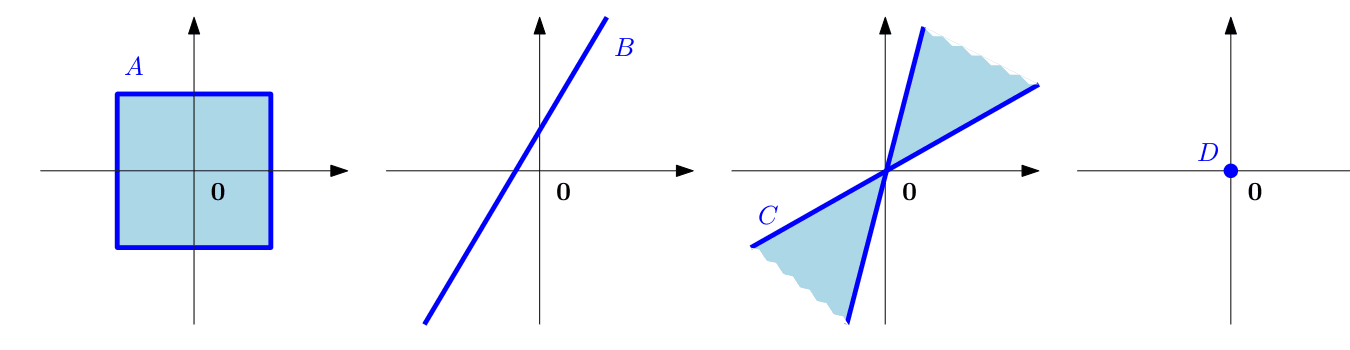
\includegraphics[width=0.92\textwidth,keepaspectratio]{docs/images/Figure2.6.png}
\caption*{\refstepcounter{figcounter}\label{fig:2-6}图~\thefigcounter 并非 R² 的所有子集都是子空间。在 A 和 C 中，违背了封闭性；B 不包含 0。只有 D 是子空间。}
\end{figure}


\emph{备注} 。每个子空间 $ U \subseteq (\mathbb{R}^n, +, \cdot) $ 都是某个关于 $ \boldsymbol{x} \in \mathbb{R}^n $ 的齐次线性方程组 $ \boldsymbol {Ax} = \boldsymbol{0} $ 的解空间。

\section*{2.5 线性无关}
\addcontentsline{toc}{section}{2.5 线性无关}
\label{sec:2.5}

在下文中，我们将仔细考察可以对向量（向量空间中的元素）进行哪些操作。具体而言，我们可以将向量相加，也可以将它们乘以标量。封闭性保证了运算的结果仍然是同一向量空间中的另一个向量。我们有可能找到一组向量，使得通过对它们进行加法和缩放运算，能够表示该向量空间中的任意向量。这组向量构成了一组 \emph{基（basis）} ，我们将在第 2.6.1 节中对此进行详细讨论。在此之前，我们需要首先引入 \emph{线性组合（linear combinations）} 与 \emph{线性无关（linear independence）} 的概念。

\textbf{定义 2.11}（线性组合）。考虑一个向量空间 $ V $ 以及有限个向量 $ \boldsymbol{x}_1, \ldots, \boldsymbol{x}_k \in V $。那么，形式如下的任意向量 $ \boldsymbol{v} \in V $：

\begin{equation}
\boldsymbol{v} = \lambda_1 \boldsymbol{x}_1 + \cdots + \lambda_k \boldsymbol{x}_k = \sum_{i=1}^k \lambda_i \boldsymbol{x}_i \in V
\tag{2.65}\label{eq:2-65}
\end{equation}

其中 $ \lambda_1, \ldots, \lambda_k \in \mathbb{R} $，称为向量 $ \boldsymbol{x}_1, \ldots, \boldsymbol{x}_k $ 的 \emph{线性组合（linear combination）} 。

零向量 $ \boldsymbol{0} $ 总是可以表示为 $ k $ 个向量 $ \boldsymbol{x}_1, \ldots, \boldsymbol{x}_k $ 的线性组合，因为 $ \boldsymbol{0} = \sum_{i=1}^k 0 \boldsymbol{x}_i $ 始终成立。在下文中，我们感兴趣的是使用一组向量表示 $ \boldsymbol{0} $ 的 \emph{非平凡线性组合（non-trivial linear combinations）} ，即系数 $ \lambda_i $ 在 (2.65) 中不全为 0 的线性组合。

\textbf{定义 2.12}（线性相关与线性无关）。考虑一个向量空间 $ V $，其中 $ k \in \mathbb{N} $ 且 $ \boldsymbol{x}_1, \ldots, \boldsymbol{x}_k \in V $。如果存在非平凡线性组合使得：

\begin{equation*}
\boldsymbol{0} = \sum_{i=1}^k \lambda_i \boldsymbol{x}_i
\end{equation*}

其中至少有一个 $ \lambda_i \neq 0 $，则称向量 $ \boldsymbol{x}_1, \ldots, \boldsymbol{x}_k $ 是 \emph{线性相关（linearly dependent）} 的。如果只存在平凡解，即：

\begin{equation*}
\lambda_1 = \ldots = \lambda_k = 0
\end{equation*}

则称向量 $ \boldsymbol{x}_1, \ldots, \boldsymbol{x}_k $ 是 \emph{线性无关（linearly independent）} 的。

线性无关是线性代数中最重要的概念之一。直观地说，一组线性无关的向量所包含的信息没有任何冗余；也就是说，如果我们从这组向量中移除任何一个向量，都会丢失一部分表达能力。在接下来的小节中，我们将进一步形式化这种直觉。

\begin{notebox}
\textbf{例 2.13（线性相关向量）}
\end{notebox}

\begin{notebox}
一个地理位置的例子有助于澄清线性无关的概念。在肯尼亚内罗毕（Nairobi），如果有人向你描述卢旺达基加利（Kigali）的位置，他可能会说：“你可以先向西北走 506 公里到达乌干达坎帕拉（Kampala），然后再向西南走 374 公里即可到达基加利。”这些信息足以描述基加利的位置，因为地理坐标系可以视为一个二维向量空间（忽略海拔高度和地球曲率）。
\end{notebox}

\begin{notebox}
这个人可能还会补充一句：“它就在这里正西方向约 751 公里处。”尽管后一句话是真实的，但在已知前述信息的情况下，它对于找到基加利并不是必需的（见图~\ref{fig:2-7} 说明）。
\end{notebox}

\begin{notebox}
在这个例子中，“向西北 506 公里”向量（蓝色）与“向西南 374 公里”向量（紫色）是线性无关的。这意味着西南向量无法由西北向量来表示，反之亦然。然而，第三个“向西 751 公里”向量（黑色）是前两个向量的线性组合，这使得这组向量构成了线性相关集。类似地，利用“向西 751 公里”和“向西南 374 公里”也可以线性组合得到“向西北 506 公里”。
\end{notebox}


\begin{figure}[H]
\centering
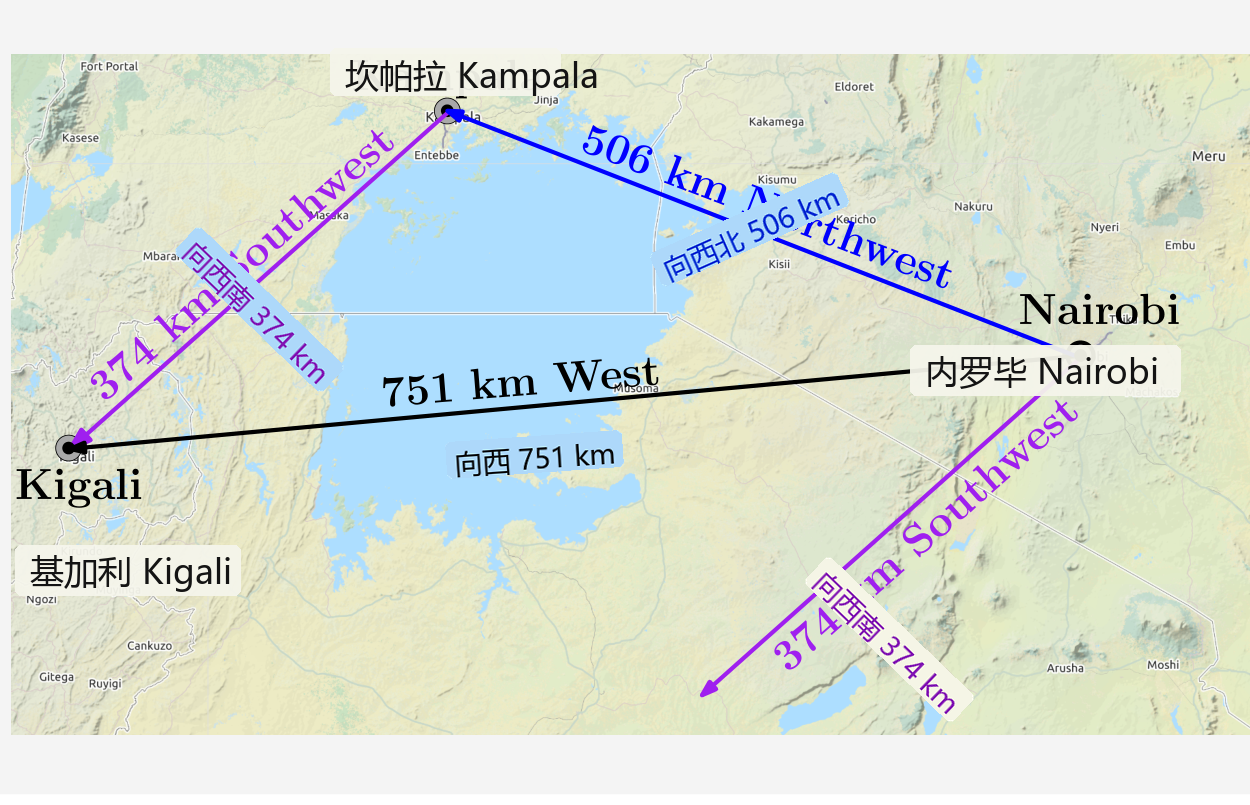
\includegraphics[width=0.92\textwidth,keepaspectratio]{docs/images/Figure2.7.png}
\caption*{\refstepcounter{figcounter}\label{fig:2-7}图~\thefigcounter 二维空间（平面）中线性相关向量的地理示例（粗略近似主要方位基向）。}
\end{figure}


\emph{备注} 。以下性质对于判断向量是否线性无关非常有用：

\begin{itemize}
\item $ k $ 个向量要么线性相关，要么线性无关，不存在第三种情况。
\item 如果向量 $ \boldsymbol{x}_1, \ldots, \boldsymbol{x}_k $ 中至少有一个是零向量 $ \boldsymbol{0} $，则它们线性相关。如果两个向量完全相同，结论同样成立。
\item 向量集合 $ \{\boldsymbol{x}_1, \ldots, \boldsymbol{x}_k : \boldsymbol{x}_i \neq \boldsymbol{0}, i = 1, \ldots, k\} $（$ k \geqslant 2 $）线性相关的充要条件是：其中（至少）有一个向量可以表示为其余向量的线性组合。特别地，如果一个向量是另一个向量的倍数（即 $ \boldsymbol{x}_i = \lambda \boldsymbol{x}_j, \lambda \in \mathbb{R} $），则该集合是线性相关的。
\end{itemize}

检验向量 $ \boldsymbol{x}_1, \ldots, \boldsymbol{x}_k \in V $ 是否线性无关的一种实用方法是使用高斯消元法：将所有向量作为矩阵 $ \boldsymbol{A} $ 的列，执行高斯消元直到该矩阵化为行阶梯形（此处不需要化为简化行阶梯形）：

\begin{itemize}
\item 主元列（pivot columns）表示与位于其左侧的向量线性无关的向量。请注意，在构建矩阵时向量之间存在先后顺序。
\item 非主元列可以表示为位于其左侧的主元列的线性组合。例如，行阶梯形： 告诉我们第一列和第三列是主元列。第二列是非主元列，因为它是第一列的 3 倍。
\end{itemize}
\begin{equation}
\begin{bmatrix} 1 & 3 & 0 \\ 0 & 0 & 2 \end{bmatrix}
\tag{2.66}\label{eq:2-66}
\end{equation}
\begin{itemize}
\item 所有列向量线性无关的充要条件是：所有列均为主元列。如果至少存在一个非主元列，则这些列（以及对应的向量）线性相关。
\end{itemize}

\begin{notebox}
\textbf{例 2.14}
\end{notebox}

\begin{notebox}
考虑 $ \mathbb{R}^4 $ 中的三个向量：

\begin{equation}
\boldsymbol{x}_1 = \begin{bmatrix} 1 \\ 2 \\ -3 \\ 4 \end{bmatrix}, \quad \boldsymbol{x}_2 = \begin{bmatrix} 1 \\ 1 \\ 0 \\ 2 \end{bmatrix}, \quad \boldsymbol{x}_3 = \begin{bmatrix} -1 \\ -2 \\ 1 \\ 1 \end{bmatrix}
\tag{2.67}\label{eq:2-67}
\end{equation}

为了检验它们是否线性相关，我们按照通用方法求解关于 $ \lambda_1, \lambda_2, \lambda_3 $ 的齐次方程：

\begin{equation}
\begin{adjustbox}{max width=\linewidth}
\lambda_1 \boldsymbol{x}_1 + \lambda_2 \boldsymbol{x}_2 + \lambda_3 \boldsymbol{x}_3 = \lambda_1 \begin{bmatrix} 1 \\ 2 \\ -3 \\ 4 \end{bmatrix} + \lambda_2 \begin{bmatrix} 1 \\ 1 \\ 0 \\ 2 \end{bmatrix} + \lambda_3 \begin{bmatrix} -1 \\ -2 \\ 1 \\ 1 \end{bmatrix} = \boldsymbol{0}
\end{adjustbox}
\tag{2.68}\label{eq:2-68}
\end{equation}

我们将向量 $ \boldsymbol{x}_i $（$ i = 1, 2, 3 $）按列拼成一个矩阵，并应用初等行变换，直到确定出主元列：

\begin{equation}
\begin{adjustbox}{max width=\linewidth}
\begin{bmatrix} 1 & 1 & -1 \\ 2 & 1 & -2 \\ -3 & 0 & 1 \\ 4 & 2 & 1 \end{bmatrix} \leadsto \cdots \leadsto \begin{bmatrix} 1 & 1 & -1 \\ 0 & 1 & 0 \\ 0 & 0 & 1 \\ 0 & 0 & 0 \end{bmatrix}
\end{adjustbox}
\tag{2.69}\label{eq:2-69}
\end{equation}

这里矩阵的每一列都是主元列。因此不存在非平凡解，解该方程组必须满足 $ \lambda_1 = 0, \lambda_2 = 0, \lambda_3 = 0 $。由此可知，向量 $ \boldsymbol{x}_1, \boldsymbol{x}_2, \boldsymbol{x}_3 $ 是线性无关的。
\end{notebox}

\emph{备注} 。考虑一个具有 $ k $ 个线性无关向量 $ \boldsymbol{b}_1, \ldots, \boldsymbol{b}_k $ 的向量空间 $ V $，以及 $ m $ 个线性组合：

\begin{equation}
\begin{aligned}
  \boldsymbol{x}_1 &= \sum_{i=1}^k \lambda_{i1} \boldsymbol{b}_i \\
  &\ \ \vdots \\
  \boldsymbol{x}_m &= \sum_{i=1}^k \lambda_{im} \boldsymbol{b}_i
\end{aligned}
\tag{2.70}\label{eq:2-70}
\end{equation}

将以这些线性无关向量 $ \boldsymbol{b}_1, \ldots, \boldsymbol{b}_k $ 为列的矩阵定义为 $ \boldsymbol{B} = [\boldsymbol{b}_1, \ldots, \boldsymbol{b}_k] $，我们可以将上述线性组合更紧凑地写为：

\begin{equation}
\boldsymbol{x}_j = \boldsymbol{B} \boldsymbol{\lambda}_j, \quad \boldsymbol{\lambda}_j = \begin{bmatrix} \lambda_{1j} \\ \vdots \\ \lambda_{kj} \end{bmatrix}, \quad j = 1, \ldots, m
\tag{2.71}\label{eq:2-71}
\end{equation}

我们想要检验 $ \boldsymbol{x}_1, \ldots, \boldsymbol{x}_m $ 是否线性无关。为此，我们按照通用方法检验何时 $ \sum_{j=1}^m \psi_j \boldsymbol{x}_j = \boldsymbol{0} $。结合 (2.71)，我们得到：

\begin{equation}
\sum_{j=1}^m \psi_j \boldsymbol{x}_j = \sum_{j=1}^m \psi_j \boldsymbol{B} \boldsymbol{\lambda}_j = \boldsymbol{B} \sum_{j=1}^m \psi_j \boldsymbol{\lambda}_j
\tag{2.72}\label{eq:2-72}
\end{equation}

这意味着，向量集合 $ \{\boldsymbol{x}_1, \ldots, \boldsymbol{x}_m\} $ 线性无关的充要条件是：列向量集合 $ \{\boldsymbol{\lambda}_1, \ldots, \boldsymbol{\lambda}_m\} $ 线性无关。

\emph{备注} 。在向量空间 $ V $ 中，$ k $ 个向量 $ \boldsymbol{x}_1, \ldots, \boldsymbol{x}_k $ 的 $ m $ 个线性组合在 $ m > k $ 时必定线性相关。

\begin{notebox}
\textbf{例 2.15}
\end{notebox}

\begin{notebox}
考虑一组线性无关的向量 $ \boldsymbol{b}_1, \boldsymbol{b}_2, \boldsymbol{b}_3, \boldsymbol{b}_4 \in \mathbb{R}^n $，以及：

\begin{equation}
\begin{adjustbox}{max width=\linewidth}
\begin{aligned}
  \boldsymbol{x}_1 &= \boldsymbol{b}_1 - 2\boldsymbol{b}_2 + \boldsymbol{b}_3 - \boldsymbol{b}_4 \\
  \boldsymbol{x}_2 &= -4\boldsymbol{b}_1 - 2\boldsymbol{b}_2 + 4\boldsymbol{b}_4 \\
  \boldsymbol{x}_3 &= 2\boldsymbol{b}_1 + 3\boldsymbol{b}_2 - \boldsymbol{b}_3 - 3\boldsymbol{b}_4 \\
  \boldsymbol{x}_4 &= 17\boldsymbol{b}_1 - 10\boldsymbol{b}_2 + 11\boldsymbol{b}_3 + \boldsymbol{b}_4
\end{aligned}
\end{adjustbox}
\tag{2.73}\label{eq:2-73}
\end{equation}

向量 $ \boldsymbol{x}_1, \ldots, \boldsymbol{x}_4 \in \mathbb{R}^n $ 是否线性无关？
\end{notebox}

\begin{notebox}
为了回答这个问题，我们研究列向量集合：

\begin{equation}
\left\{ \begin{bmatrix} 1 \\ -2 \\ 1 \\ -1 \end{bmatrix}, \begin{bmatrix} -4 \\ -2 \\ 0 \\ 4 \end{bmatrix}, \begin{bmatrix} 2 \\ 3 \\ -1 \\ -3 \end{bmatrix}, \begin{bmatrix} 17 \\ -10 \\ 11 \\ 1 \end{bmatrix} \right\}
\tag{2.74}\label{eq:2-74}
\end{equation}

是否线性无关。对应线性方程组的系数矩阵为：

\begin{equation}
\begin{adjustbox}{max width=\linewidth}
\boldsymbol{A} = \begin{bmatrix} 1 & -4 & 2 & 17 \\ -2 & -2 & 3 & -10 \\ 1 & 0 & -1 & 11 \\ -1 & 4 & -3 & 1 \end{bmatrix}
\end{adjustbox}
\tag{2.75}\label{eq:2-75}
\end{equation}

将其化为简化行阶梯形矩阵，结果为：

\begin{equation}
\begin{adjustbox}{max width=\linewidth}
\begin{bmatrix} 1 & 0 & 0 & -7 \\ 0 & 1 & 0 & -15 \\ 0 & 0 & 1 & -18 \\ 0 & 0 & 0 & 0 \end{bmatrix}
\end{adjustbox}
\tag{2.76}\label{eq:2-76}
\end{equation}

我们看到对应的线性方程组具有非平凡解：最后一列不是主元列，并且 $ \boldsymbol{x}_4 = -7\boldsymbol{x}_1 - 15\boldsymbol{x}_2 - 18\boldsymbol{x}_3 $。因此，$ \boldsymbol{x}_1, \ldots, \boldsymbol{x}_4 $ 是线性相关的，因为 $ \boldsymbol{x}_4 $ 可以表示为 $ \boldsymbol{x}_1, \ldots, \boldsymbol{x}_3 $ 的线性组合。
\end{notebox}

\section*{2.6 基和秩}
\addcontentsline{toc}{section}{2.6 基和秩}
\label{sec:2.6}

在向量空间 $ V $ 中，我们对这样一类向量集合 $ A $ 尤其感兴趣：它们具备使得 $ V $ 中的任意向量 $ \boldsymbol{v} $ 均可通过 $ A $ 中向量的线性组合来获得的性质。这些向量属于特殊向量，在下文中我们将对其性质进行刻画。

\section*{2.6.1 生成集与基}
\addcontentsline{toc}{subsection}{2.6.1 生成集与基}

\textbf{定义 2.13}（生成集与张成空间）。考虑一个向量空间 $ V = (V, +, \cdot) $ 以及向量集合 $ A = \{\boldsymbol{x}_1, \ldots, \boldsymbol{x}_k\} \subseteq V $。如果 $ V $ 中的每一个向量 $ \boldsymbol{v} $ 都可以表示为 $ \boldsymbol{x}_1, \ldots, \boldsymbol{x}_k $ 的线性组合，则称 $ A $ 为 $ V $ 的 \emph{生成集（generating set）} 。由 $ A $ 中向量的所有线性组合构成的集合称为 $ A $ 的 \emph{张成空间（span）} 。如果 $ A $ 张成了向量空间 $ V $，我们记作 $ V = \operatorname{span}[A] $ 或 $ V = \operatorname{span}[\boldsymbol{x}_1, \ldots, \boldsymbol{x}_k] $。

生成集是张成整个向量（子）空间的向量集合，即该空间中的每个向量都可以表示为生成集中向量的线性组合。现在，我们将更加具体地刻画张成一个向量（子）空间的“最小”生成集。

\textbf{定义 2.14}（基）。考虑一个向量空间 $ V = (V, +, \cdot) $ 及其子集 $ A \subseteq V $。如果不存在能够张成 $ V $ 且比 $ A $ 更小的集合 $ \tilde{A} \subsetneq A \subseteq V $，则称 $ V $ 的生成集 $ A $ 是 \emph{极小的（minimal）} 。$ V $ 的每一个线性无关的生成集都是极小的，并称为 $ V $ 的一组 \emph{基（basis）} 。

设 $ V = (V, +, \cdot) $ 为一个向量空间，且 $ B \subseteq V, B \neq \emptyset $。那么，以下陈述是等价的：

\begin{itemize}
\item $ B $ 是 $ V $ 的一组基。
\item $ B $ 是一个极小生成集。
\item $ B $ 是 $ V $ 中的极大线性无关向量集，即向该集合中添加任何其他向量都会使其变为线性相关的。
\item $ V $ 中的每一个向量 $ \boldsymbol{x} $ 都是来自 $ B $ 中向量的线性组合，且每个线性组合都是唯一的，即由： 且 $ \lambda_i, \psi_i \in \mathbb{R}, \boldsymbol{b}_i \in B $，可推导出对所有 $ i = 1, \ldots, k $ 均有 $ \lambda_i = \psi_i $。
\end{itemize}
\begin{equation}
\boldsymbol{x} = \sum_{i=1}^k \lambda_i \boldsymbol{b}_i = \sum_{i=1}^k \psi_i \boldsymbol{b}_i
\tag{2.77}\label{eq:2-77}
\end{equation}
\begin{itemize}
\end{itemize}

\begin{notebox}
一组基既是一个极小生成集，也是一个极大线性无关向量集合。
\end{notebox}

\begin{notebox}
\textbf{例 2.16}
\end{notebox}

\begin{notebox}
在 $ \mathbb{R}^3 $ 中， \emph{标准基（canonical/standard basis）} 为：

\begin{equation}
B = \left\{ \begin{bmatrix} 1 \\ 0 \\ 0 \end{bmatrix}, \begin{bmatrix} 0 \\ 1 \\ 0 \end{bmatrix}, \begin{bmatrix} 0 \\ 0 \\ 1 \end{bmatrix} \right\}
\tag{2.78}\label{eq:2-78}
\end{equation}

$ \mathbb{R}^3 $ 中的其他不同基例如：

\begin{equation}
\begin{adjustbox}{max width=\linewidth}
B_1 = \left\{ \begin{bmatrix} 1 \\ 0 \\ 0 \end{bmatrix}, \begin{bmatrix} 1 \\ 1 \\ 0 \end{bmatrix}, \begin{bmatrix} 1 \\ 1 \\ 1 \end{bmatrix} \right\}, \quad B_2 = \left\{ \begin{bmatrix} 0.5 \\ 0.8 \\ 0.4 \end{bmatrix}, \begin{bmatrix} 1.8 \\ 0.3 \\ 0.3 \end{bmatrix}, \begin{bmatrix} -2.2 \\ -1.3 \\ 3.5 \end{bmatrix} \right\}
\end{adjustbox}
\tag{2.79}\label{eq:2-79}
\end{equation}

而集合：

\begin{equation}
A = \left\{ \begin{bmatrix} 1 \\ 2 \\ 3 \\ 4 \end{bmatrix}, \begin{bmatrix} 2 \\ -1 \\ 0 \\ 2 \end{bmatrix}, \begin{bmatrix} 1 \\ 1 \\ 0 \\ -4 \end{bmatrix} \right\}
\tag{2.80}\label{eq:2-80}
\end{equation}

是线性无关的，但它不是 $ \mathbb{R}^4 $ 的生成集（也不是基）：例如向量 $ [1, 0, 0, 0]^\top $ 无法由 $ A $ 中元素的线性组合获得。
\end{notebox}

\emph{备注} 。每个向量空间 $ V $ 都拥有一组基 $ B $。上述例子表明一个向量空间 $ V $ 可以存在很多组基，即基并不是唯一的。然而，所有的基都拥有相同数量的元素，即 \emph{基向量（basis vectors）} 。

我们只考虑有限维向量空间 $ V $。在这种情况下，$ V $ 的 \emph{维度（dimension）} 等于 $ V $ 的基向量数量，记为 $ \operatorname{dim}(V) $。如果 $ U \subseteq V $ 是 $ V $ 的一个子空间，则 $ \operatorname{dim}(U) \leqslant \operatorname{dim}(V) $，且当且仅当 $ U = V $ 时 $ \operatorname{dim}(U) = \operatorname{dim}(V) $。直观地，向量空间的维度可以看作该向量空间中独立方向的数量。

\begin{notebox}
向量空间的维度对应于其基向量的数量。
\end{notebox}

\emph{备注} 。向量空间的维度并不必然等于向量中元素的个数。例如，向量空间

\begin{equation*}
V = \operatorname{span}\left[\begin{bmatrix} 0 \\ 1 \end{bmatrix}\right]
\end{equation*}

是一维的，尽管其基向量包含两个元素。

\emph{备注} 。求由向量张成的子空间 $ U = \operatorname{span}[\boldsymbol{x}_1, \ldots, \boldsymbol{x}_m] \subseteq \mathbb{R}^n $ 的一组基，可以通过执行以下步骤完成：

\begin{enumerate}
\item 将张成向量作为矩阵 $ \boldsymbol{A} $ 的列写入；
\item 确定 $ \boldsymbol{A} $ 的行阶梯形矩阵；
\item 与主元列相关联的原张成向量即构成 $ U $ 的一组基。
\end{enumerate}

\begin{notebox}
\textbf{例 2.17（确定一组基）}
\end{notebox}

\begin{notebox}
对于由以下向量张成的向量子空间 $ U \subseteq \mathbb{R}^5 $：

\begin{equation}
\begin{adjustbox}{max width=\linewidth}
\boldsymbol{x}_1 = \begin{bmatrix} 1 \\ 2 \\ -1 \\ -1 \\ -1 \end{bmatrix}, \quad \boldsymbol{x}_2 = \begin{bmatrix} 2 \\ -1 \\ 1 \\ 2 \\ -2 \end{bmatrix}, \quad \boldsymbol{x}_3 = \begin{bmatrix} 3 \\ -4 \\ 3 \\ 5 \\ -3 \end{bmatrix}, \quad \boldsymbol{x}_4 = \begin{bmatrix} -1 \\ 8 \\ -5 \\ -6 \\ 1 \end{bmatrix} \in \mathbb{R}^5
\end{adjustbox}
\tag{2.81}\label{eq:2-81}
\end{equation}

我们想要找出向量 $ \boldsymbol{x}_1, \ldots, \boldsymbol{x}_4 $ 中哪些构成了 $ U $ 的一组基。为此，我们需要检验 $ \boldsymbol{x}_1, \ldots, \boldsymbol{x}_4 $ 是否线性无关。因此，我们需要求解：

\begin{equation}
\sum_{i=1}^4 \lambda_i \boldsymbol{x}_i = \boldsymbol{0}
\tag{2.82}\label{eq:2-82}
\end{equation}

这导出了以如下矩阵为系数矩阵的齐次线性方程组：

\begin{equation}
\begin{adjustbox}{max width=\linewidth}
[\boldsymbol{x}_1, \boldsymbol{x}_2, \boldsymbol{x}_3, \boldsymbol{x}_4] = \begin{bmatrix} 1 & 2 & 3 & -1 \\ 2 & -1 & -4 & 8 \\ -1 & 1 & 3 & -5 \\ -1 & 2 & 5 & -6 \\ -1 & -2 & -3 & 1 \end{bmatrix}
\end{adjustbox}
\tag{2.83}\label{eq:2-83}
\end{equation}

利用线性方程组的初等变换规则，我们得到行阶梯形矩阵：

\begin{equation*}
\begin{adjustbox}{max width=\linewidth}
\begin{bmatrix} 1 & 2 & 3 & -1 \\ 2 & -1 & -4 & 8 \\ -1 & 1 & 3 & -5 \\ -1 & 2 & 5 & -6 \\ -1 & -2 & -3 & 1 \end{bmatrix} \leadsto \cdots \leadsto \begin{bmatrix} 1 & 2 & 3 & -1 \\ 0 & 1 & 2 & -2 \\ 0 & 0 & 0 & 1 \\ 0 & 0 & 0 & 0 \\ 0 & 0 & 0 & 0 \end{bmatrix}
\end{adjustbox}
\end{equation*}

由于主元列指示了哪些向量构成线性无关集，从行阶梯形中我们可以看出第 1、2、4 列为主元列，因此 $ \boldsymbol{x}_1, \boldsymbol{x}_2, \boldsymbol{x}_4 $ 是线性无关的（因为线性方程组 $ \lambda_1 \boldsymbol{x}_1 + \lambda_2 \boldsymbol{x}_2 + \lambda_4 \boldsymbol{x}_4 = \boldsymbol{0} $ 只有平凡解 $ \lambda_1 = \lambda_2 = \lambda_4 = 0 $）。因此，$ \{\boldsymbol{x}_1, \boldsymbol{x}_2, \boldsymbol{x}_4\} $ 是 $ U $ 的一组基。
\end{notebox}

\medskip\hrule\medskip

\section*{2.6.2 秩}
\addcontentsline{toc}{subsection}{2.6.2 秩}

矩阵 $ \boldsymbol{A} \in \mathbb{R}^{m \times n} $ 的线性无关列的数量等于其线性无关行的数量，并称为 $ \boldsymbol{A} $ 的 \emph{秩（rank）} ，记为 $ \operatorname{rk}(\boldsymbol{A}) $。

\emph{备注} 。矩阵的秩具有一些重要性质：

\begin{itemize}
\item $ \operatorname{rk}(\boldsymbol{A}) = \operatorname{rk}(\boldsymbol{A}^\top) $，即列秩等于行秩。
\item $ \boldsymbol{A} \in \mathbb{R}^{m \times n} $ 的列张成了 $ \mathbb{R}^m $ 的一个子空间 $ U \subseteq \mathbb{R}^m $，且 $ \operatorname{dim}(U) = \operatorname{rk}(\boldsymbol{A}) $。稍后我们将这个子空间称为 \emph{像（image）} 或 \emph{值域（range）} 。通过对 $ \boldsymbol{A} $ 执行高斯消元以确定主元列，可以求出 $ U $ 的一组基。
\item $ \boldsymbol{A} \in \mathbb{R}^{m \times n} $ 的行张成了 $ \mathbb{R}^n $ 的一个子空间 $ W \subseteq \mathbb{R}^n $，且 $ \operatorname{dim}(W) = \operatorname{rk}(\boldsymbol{A}) $。通过对 $ \boldsymbol{A}^\top $ 执行高斯消元，可以求出 $ W $ 的一组基。
\item 对于所有方阵 $ \boldsymbol{A} \in \mathbb{R}^{n \times n} $，$ \boldsymbol{A} $ 正则（可逆）当且仅当 $ \operatorname{rk}(\boldsymbol{A}) = n $。
\item 对于所有 $ \boldsymbol{A} \in \mathbb{R}^{m \times n} $ 和所有 $ \boldsymbol{b} \in \mathbb{R}^m $，线性方程组 $ \boldsymbol {Ax} = \boldsymbol{b} $ 有解当且仅当 $ \operatorname{rk}(\boldsymbol{A}) = \operatorname{rk}([\boldsymbol{A} \mid \boldsymbol{b}]) $，其中 $ [\boldsymbol{A} \mid \boldsymbol{b}] $ 表示增广矩阵。
\item 对于 $ \boldsymbol{A} \in \mathbb{R}^{m \times n} $，$ \boldsymbol {Ax} = \boldsymbol{0} $ 的解空间（子空间）的维度为 $ n - \operatorname{rk}(\boldsymbol{A}) $。稍后我们称这个子空间为 \emph{核（kernel）} 或 \emph{零空间（null space）} 。
\item 若矩阵 $ \boldsymbol{A} \in \mathbb{R}^{m \times n} $ 的秩等于相同维度矩阵所可能具有的最大秩，则称其为 \emph{满秩（full rank）} 。这意味着满秩矩阵的秩等于行数和列数中的较小者，即 $ \operatorname{rk}(\boldsymbol{A}) = \min(m, n) $。若矩阵不具有满秩，则称为 \emph{降秩（rank deficient）} 。
\end{itemize}

\begin{notebox}
\textbf{例 2.18（秩）}
\end{notebox}

\begin{notebox}
考察矩阵：

\begin{equation*}
\boldsymbol{A} = \begin{bmatrix} 1 & 0 & 1 \\ 0 & 1 & 1 \\ 0 & 0 & 0 \end{bmatrix}
\end{equation*}

$ \boldsymbol{A} $ 拥有两个线性无关的行/列，因此 $ \operatorname{rk}(\boldsymbol{A}) = 2 $。
\end{notebox}

\begin{notebox}
再考察矩阵：

\begin{equation*}
\boldsymbol{A} = \begin{bmatrix} 1 & 2 & 1 \\ -2 & -3 & 1 \\ 3 & 5 & 0 \end{bmatrix}
\end{equation*}

我们使用高斯消元法来确定其秩：

\begin{equation}
\begin{adjustbox}{max width=\linewidth}
\begin{bmatrix} 1 & 2 & 1 \\ -2 & -3 & 1 \\ 3 & 5 & 0 \end{bmatrix} \leadsto \cdots \leadsto \begin{bmatrix} 1 & 2 & 1 \\ 0 & 1 & 3 \\ 0 & 0 & 0 \end{bmatrix}
\end{adjustbox}
\tag{2.84}\label{eq:2-84}
\end{equation}

这里我们看到线性无关的行数和列数为 2，因此 $ \operatorname{rk}(\boldsymbol{A}) = 2 $。
\end{notebox}

\section*{2.7 线性映射}
\addcontentsline{toc}{section}{2.7 线性映射}
\label{sec:2.7}

在下文中，我们将研究向量空间上保持其结构的映射，这将使我们能够定义坐标的概念。在本章开头，我们说过向量是可以相加并且可以与标量相乘的对象，并且运算的结果仍然是一个向量。我们希望在应用映射时保持这一性质：

考虑两个实数向量空间 $ V, W $。如果一个映射 $ \Phi : V \to W $ 满足：

\begin{equation}
\Phi(\boldsymbol{x} + \boldsymbol{y}) = \Phi(\boldsymbol{x}) + \Phi(\boldsymbol{y})
\tag{2.85}\label{eq:2-85}
\end{equation}

\begin{equation}
\Phi(\lambda \boldsymbol{x}) = \lambda \Phi(\boldsymbol{x})
\tag{2.86}\label{eq:2-86}
\end{equation}

对所有 $ \boldsymbol{x}, \boldsymbol{y} \in V $ 以及 $ \lambda \in \mathbb{R} $ 均成立，则称其保持了向量空间的结构。我们可以将其总结在以下定义中：

\textbf{定义 2.15}（线性映射）。对于向量空间 $ V, W $，一个映射 $ \Phi : V \to W $ 如果满足：

\begin{equation}
\forall \boldsymbol{x}, \boldsymbol{y} \in V \ \forall \lambda, \psi \in \mathbb{R} : \Phi(\lambda \boldsymbol{x} + \psi \boldsymbol{y}) = \lambda \Phi(\boldsymbol{x}) + \psi \Phi(\boldsymbol{y})
\tag{2.87}\label{eq:2-87}
\end{equation}

则称为 \emph{线性映射（linear mapping）} （或 \emph{向量空间同态（vector space homomorphism）} 、 \emph{线性变换（linear transformation）} ）。

事实证明，我们可以将线性映射表示为矩阵（第 2.7.1 节）。回顾前面，我们也可以将一组向量收集为矩阵的列。在处理矩阵时，我们必须牢记该矩阵所代表的含义：它是一个线性映射，还是一组向量的集合。在第 4 章中，我们将看到更多关于线性映射的内容。在继续之前，我们简要介绍一些特殊的映射类型。

\textbf{定义 2.16}（单射、满射、双射）。考虑映射 $ \Phi : V \to W $，其中 $ V, W $ 可以是任意集合。那么，如果满足：

\begin{itemize}
\item \emph{单射（injective）} ：$ \forall \boldsymbol{x}, \boldsymbol{y} \in V : \Phi(\boldsymbol{x}) = \Phi(\boldsymbol{y}) \implies \boldsymbol{x} = \boldsymbol{y} $。
\item \emph{满射（surjective）} ：$ \Phi(V) = W $。
\item \emph{双射（bijective）} ：$ \Phi $ 既是单射又是满射。
\end{itemize}

如果 $ \Phi $ 是满射，那么 $ W $ 中的每一个元素都可以通过 $ \Phi $ 从 $ V $ 中“到达”。双射映射是可以“撤销”的，即存在一个映射 $ \Psi : W \to V $ 满足 $ \Psi \circ \Phi(\boldsymbol{x}) = \boldsymbol{x} $。这个映射 $ \Psi $ 称为 $ \Phi $ 的 \emph{逆映射（inverse）} ，通常记作 $ \Phi^{-1} $。

基于这些定义，我们引入向量空间 $ V $ 与 $ W $ 之间线性映射的以下特殊情形：

\begin{itemize}
\item \emph{同构（isomorphism）} ：$ \Phi : V \to W $ 是线性的且是双射。
\item \emph{自同态（endomorphism）} ：$ \Phi : V \to V $ 是线性的。
\item \emph{自同构（automorphism）} ：$ \Phi : V \to V $ 是线性的且是双射。
\item 我们将 $ \operatorname{id}_V : V \to V, \boldsymbol{x} \mapsto \boldsymbol{x} $ 定义为 $ V $ 中的 \emph{恒等映射（identity mapping）} 或 \emph{恒等自同构（identity automorphism）} 。
\end{itemize}

\begin{notebox}
\textbf{例 2.19（同态）}
\end{notebox}

\begin{notebox}
映射 $ \Phi : \mathbb{R}^2 \to \mathbb{C}, \Phi(\boldsymbol{x}) = x_1 + i x_2 $ 是一个同态：

\begin{equation*}
\begin{adjustbox}{max width=\linewidth}
\Phi\left( \begin{bmatrix} x_1 \\ x_2 \end{bmatrix} + \begin{bmatrix} y_1 \\ y_2 \end{bmatrix} \right) = (x_1 + y_1) + i(x_2 + y_2) = x_1 + i x_2 + y_1 + i y_2 = \Phi\left( \begin{bmatrix} x_1 \\ x_2 \end{bmatrix} \right) + \Phi\left( \begin{bmatrix} y_1 \\ y_2 \end{bmatrix} \right)
\end{adjustbox}
\end{equation*}

\begin{equation}
\Phi\left( \lambda \begin{bmatrix} x_1 \\ x_2 \end{bmatrix} \right) = \lambda x_1 + \lambda i x_2 = \lambda (x_1 + i x_2) = \lambda \Phi\left( \begin{bmatrix} x_1 \\ x_2 \end{bmatrix} \right)
\tag{2.88}\label{eq:2-88}
\end{equation}

这也解释了为什么复数可以表示为 $ \mathbb{R}^2 $ 中的二元元组：存在一个双射线性映射，将 $ \mathbb{R}^2 $ 中元组的按元素加法转化为带有相应加法运算的复数集合。注意这里我们仅展示了线性性质，未证明双射性。
\end{notebox}

\textbf{定理 2.17}（有限维空间同构定理，引自 Axler (2015) 定理 3.59）。有限维向量空间 $ V $ 与 $ W $ 同构当且仅当 $ \operatorname{dim}(V) = \operatorname{dim}(W) $。

定理 2.17 表明，在相同维度的两个向量空间之间存在线性双射映射。直观地说，这意味着相同维度的向量空间本质上是“同一类事物”，因为它们可以在不产生任何信息损失的情况下相互转换。

定理 2.17 也为我们将 $ \mathbb{R}^{m \times n} $（$ m \times n $ 矩阵的向量空间）与 $ \mathbb{R}^{mn} $（长度为 $ mn $ 的向量空间）视为等同提供了理论依据：它们的维度都是 $ mn $，并且存在将二者相互转换的线性双射映射。

\emph{备注} 。考虑向量空间 $ V, W, X $，则：

\begin{itemize}
\item 对于线性映射 $ \Phi : V \to W $ 与 $ \Psi : W \to X $，复合映射 $ \Psi \circ \Phi : V \to X $ 也是线性的。
\item 如果 $ \Phi : V \to W $ 是一个同构，则 $ \Phi^{-1} : W \to V $ 也是一个同构。
\item 如果 $ \Phi : V \to W $ 与 $ \Psi : V \to W $ 是线性的，则 $ \Phi + \Psi $ 以及 $ \lambda \Phi $（$ \lambda \in \mathbb{R} $）也是线性的。
\end{itemize}

\medskip\hrule\medskip

\section*{2.7.1 线性映射的矩阵表示}
\addcontentsline{toc}{subsection}{2.7.1 线性映射的矩阵表示}

任何 $ n $ 维向量空间都同构于 $ \mathbb{R}^n $（定理 2.17）。我们考虑 $ n $ 维向量空间 $ V $ 的一组基 $ \{\boldsymbol{b}_1, \ldots, \boldsymbol{b}_n\} $。在下文中，基向量的顺序将十分重要。因此，我们记：

\begin{equation}
B = (\boldsymbol{b}_1, \ldots, \boldsymbol{b}_n)
\tag{2.89}\label{eq:2-89}
\end{equation}

并称这个 $ n $ 元组为 $ V $ 的一组 \emph{有序基（ordered basis）} 。

\emph{备注} （记号区分）。我们在记号上做如下明确约定：$ B = (\boldsymbol{b}_1, \ldots, \boldsymbol{b}_n) $ 表示有序基，$ B = \{\boldsymbol{b}_1, \ldots, \boldsymbol{b}_n\} $ 表示（无序的）基集合，而 $ \boldsymbol{B} = [\boldsymbol{b}_1, \ldots, \boldsymbol{b}_n] $ 表示以向量 $ \boldsymbol{b}_1, \ldots, \boldsymbol{b}_n $ 为列构成的矩阵。

\textbf{定义 2.18}（坐标）。考虑一个向量空间 $ V $ 以及 $ V $ 的一组有序基 $ B = (\boldsymbol{b}_1, \ldots, \boldsymbol{b}_n) $。对于任意 $ \boldsymbol{x} \in V $，我们都可以得到 $ \boldsymbol{x} $ 关于 $ B $ 的唯一表示（线性组合）：

\begin{equation}
\boldsymbol{x} = \alpha_1 \boldsymbol{b}_1 + \cdots + \alpha_n \boldsymbol{b}_n
\tag{2.90}\label{eq:2-90}
\end{equation}

此时 $ \alpha_1, \ldots, \alpha_n $ 称为 $ \boldsymbol{x} $ 关于 $ B $ 的 \emph{坐标（coordinates）} ，向量：

\begin{equation}
\boldsymbol{\alpha} = \begin{bmatrix} \alpha_1 \\ \vdots \\ \alpha_n \end{bmatrix} \in \mathbb{R}^n
\tag{2.91}\label{eq:2-91}
\end{equation}

称为 $ \boldsymbol{x} $ 关于有序基 $ B $ 的 \emph{坐标向量（coordinate vector）} 或 \emph{坐标表示（coordinate representation）} 。

一组基实际上定义了一个坐标系。我们所熟知的二维笛卡尔坐标系就是由标准基向量 $ \boldsymbol{e}_1, \boldsymbol{e}_2 $ 张成的。在这个坐标系中，向量 $ \boldsymbol{x} \in \mathbb{R}^2 $ 的表示告诉我们如何线性组合 $ \boldsymbol{e}_1 $ 和 $ \boldsymbol{e}_2 $ 来获得 $ \boldsymbol{x} $。然而，$ \mathbb{R}^2 $ 的任意一组基都定义了一个合法的坐标系，先前同一个向量 $ \boldsymbol{x} $ 在基 $ (\boldsymbol{b}_1, \boldsymbol{b}_2) $ 下可能具有不同的坐标表示。在图~\ref{fig:2-8} 中，向量 $ \boldsymbol{x} $ 关于标准基 $ (\boldsymbol{e}_1, \boldsymbol{e}_2) $ 的坐标是 $ [2, 2]^\top $；然而，关于基 $ (\boldsymbol{b}_1, \boldsymbol{b}_2) $，同一个向量 $ \boldsymbol{x} $ 的表示为 $ [1.09, 0.72]^\top $，即 $ \boldsymbol{x} = 1.09 \boldsymbol{b}_1 + 0.72 \boldsymbol{b}_2 $。在接下来的小节中，我们将探究如何求得这种表示。


\begin{figure}[H]
\centering
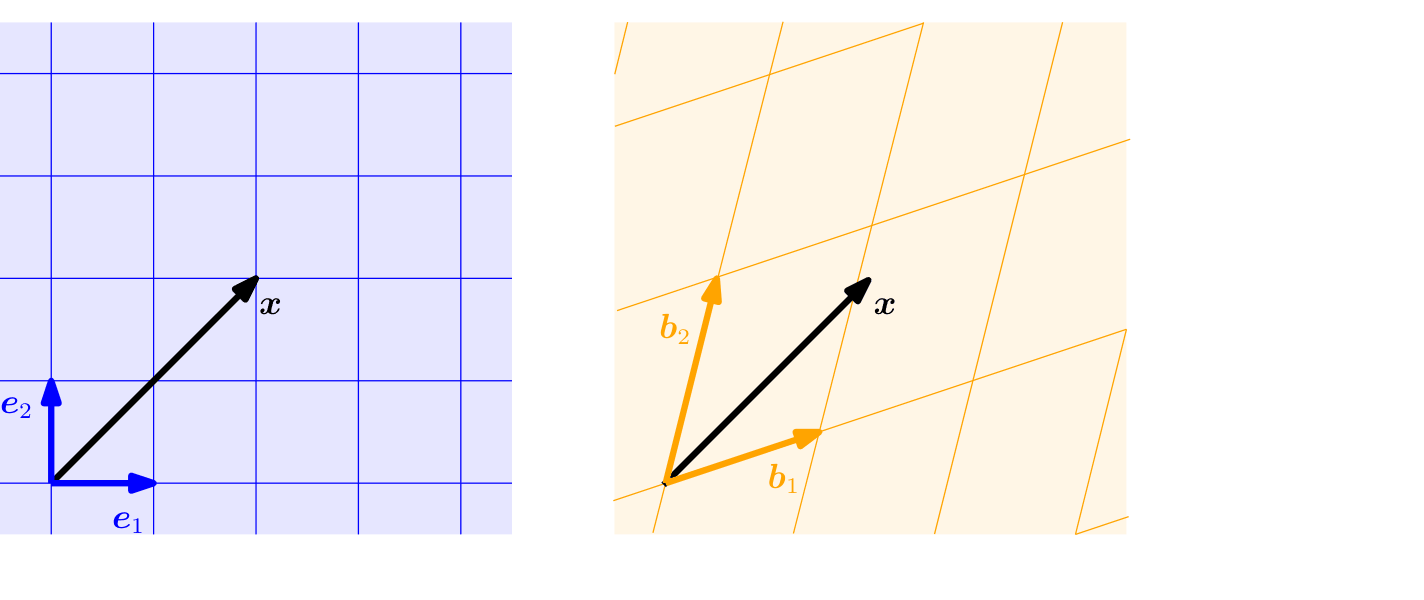
\includegraphics[width=0.92\textwidth,keepaspectratio]{docs/images/Figure2.8.png}
\caption*{\refstepcounter{figcounter}\label{fig:2-8}图~\thefigcounter 根据基的不同选择，向量 x 的两种不同坐标表示。}
\end{figure}


\begin{notebox}
\textbf{例 2.20}
\end{notebox}

\begin{notebox}
让我们考察一个几何向量 $ \boldsymbol{x} \in \mathbb{R}^2 $，它关于 $ \mathbb{R}^2 $ 的标准基 $ (\boldsymbol{e}_1, \boldsymbol{e}_2) $ 的坐标为 $ [2, 3]^\top $。这意味着我们可以写作 $ \boldsymbol{x} = 2\boldsymbol{e}_1 + 3\boldsymbol{e}_2 $。然而，我们并不一定要选择标准基来表示这个向量。如果我们使用基向量 $ \boldsymbol{b}_1 = [1, -1]^\top, \boldsymbol{b}_2 = [1, 1]^\top $，我们将得到坐标 $ \frac{1}{2}[-1, 5]^\top $ 来表示基 $ (\boldsymbol{b}_1, \boldsymbol{b}_2) $ 下的同一个向量（见图~\ref{fig:2-9}）。
\end{notebox}


\begin{figure}[H]
\centering
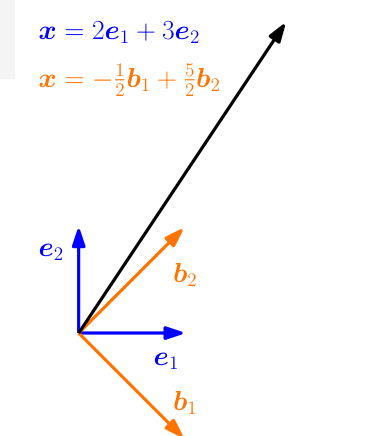
\includegraphics[width=320pt,keepaspectratio]{docs/images/Figure2.9.png}
\caption*{\refstepcounter{figcounter}\label{fig:2-9}图~\thefigcounter 向量 x 随基的选择而产生的不同坐标表示。}
\end{figure}


\emph{备注} 。对于 $ n $ 维向量空间 $ V $ 以及 $ V $ 的一组有序基 $ B $，映射 $ \Phi : \mathbb{R}^n \to V, \Phi(\boldsymbol{e}_i) = \boldsymbol{b}_i, i = 1, \ldots, n $ 是线性的（且根据定理 2.17 是一个同构），其中 $ (\boldsymbol{e}_1, \ldots, \boldsymbol{e}_n) $ 是 $ \mathbb{R}^n $ 的标准基。

现在，我们准备在有限维向量空间之间的矩阵和线性映射之间建立明确的联系。

\textbf{定义 2.19}（变换矩阵）。考虑向量空间 $ V, W $ 以及相应的有序基 $ B = (\boldsymbol{b}_1, \ldots, \boldsymbol{b}_n) $ 和 $ C = (\boldsymbol{c}_1, \ldots, \boldsymbol{c}_m) $。此外，考虑线性映射 $ \Phi : V \to W $。对于 $ j \in \{1, \ldots, n\} $：

\begin{equation}
\Phi(\boldsymbol{b}_j) = \alpha_{1j}\boldsymbol{c}_1 + \cdots + \alpha_{mj}\boldsymbol{c}_m = \sum_{i=1}^m \alpha_{ij}\boldsymbol{c}_i
\tag{2.92}\label{eq:2-92}
\end{equation}

是 $ \Phi(\boldsymbol{b}_j) $ 关于 $ C $ 的唯一表示。此时，我们称元素由下式给出的 $ m \times n $ 矩阵 $ \boldsymbol{A}_\Phi $：

\begin{equation}
\boldsymbol{A}_\Phi(i, j) = \alpha_{ij}
\tag{2.93}\label{eq:2-93}
\end{equation}

为 $ \Phi $（关于 $ V $ 的有序基 $ B $ 和 $ W $ 的有序基 $ C $ 的） \emph{变换矩阵（transformation matrix）} 。

$ \Phi(\boldsymbol{b}_j) $ 关于 $ W $ 的有序基 $ C $ 的坐标正是 $ \boldsymbol{A}_\Phi $ 的第 $ j $ 列。考虑具有有序基 $ B, C $ 的有限维向量空间 $ V, W $ 以及具有变换矩阵 $ \boldsymbol{A}_\Phi $ 的线性映射 $ \Phi : V \to W $。若 $ \hat{\boldsymbol{x}} $ 是 $ \boldsymbol{x} \in V $ 关于 $ B $ 的坐标向量，且 $ \hat{\boldsymbol{y}} $ 是 $ \boldsymbol{y} = \Phi(\boldsymbol{x}) \in W $ 关于 $ C $ 的坐标向量，则：

\begin{equation}
\hat{\boldsymbol{y}} = \boldsymbol{A}_\Phi \hat{\boldsymbol{x}}
\tag{2.94}\label{eq:2-94}
\end{equation}

这意味着变换矩阵可用于将关于 $ V $ 中有序基的坐标映射到关于 $ W $ 中有序基的坐标。

\begin{notebox}
\textbf{例 2.21（变换矩阵）}
\end{notebox}

\begin{notebox}
考虑同态 $ \Phi : V \to W $ 以及 $ V $ 的有序基 $ B = (\boldsymbol{b}_1, \ldots, \boldsymbol{b}_3) $ 和 $ W $ 的有序基 $ C = (\boldsymbol{c}_1, \ldots, \boldsymbol{c}_4) $。已知：

\begin{equation}
\begin{adjustbox}{max width=\linewidth}
\begin{aligned}
  \Phi(\boldsymbol{b}_1) &= \boldsymbol{c}_1 - \boldsymbol{c}_2 + 3\boldsymbol{c}_3 - \boldsymbol{c}_4 \\
  \Phi(\boldsymbol{b}_2) &= 2\boldsymbol{c}_1 + \boldsymbol{c}_2 + 7\boldsymbol{c}_3 + 2\boldsymbol{c}_4 \\
  \Phi(\boldsymbol{b}_3) &= 3\boldsymbol{c}_2 + \boldsymbol{c}_3 + 4\boldsymbol{c}_4
\end{aligned}
\end{adjustbox}
\tag{2.95}\label{eq:2-95}
\end{equation}

关于基 $ B $ 与 $ C $ 的变换矩阵 $ \boldsymbol{A}_\Phi $ 满足对 $ k = 1, \ldots, 3 $ 有 $ \Phi(\boldsymbol{b}_k) = \sum_{i=1}^4 \alpha_{ik}\boldsymbol{c}_i $，其形式为：

\begin{equation}
\boldsymbol{A}_\Phi = [\boldsymbol{\alpha}_1, \boldsymbol{\alpha}_2, \boldsymbol{\alpha}_3] = \begin{bmatrix} 1 & 2 & 0 \\ -1 & 1 & 3 \\ 3 & 7 & 1 \\ -1 & 2 & 4 \end{bmatrix}
\tag{2.96}\label{eq:2-96}
\end{equation}

其中 $ \boldsymbol{\alpha}_j $（$ j = 1, 2, 3 $）是 $ \Phi(\boldsymbol{b}_j) $ 关于 $ C $ 的坐标向量。
\end{notebox}

\begin{notebox}
\textbf{例 2.22（向量的线性变换）}
\end{notebox}

\begin{notebox}
我们考虑 $ \mathbb{R}^2 $ 中一组向量的三种线性变换，对应的变换矩阵分别为：

\begin{equation}
\begin{adjustbox}{max width=\linewidth}
\boldsymbol{A}_1 = \begin{bmatrix} \cos(\frac{\pi}{4}) & -\sin(\frac{\pi}{4}) \\ \sin(\frac{\pi}{4}) & \cos(\frac{\pi}{4}) \end{bmatrix}, \quad \boldsymbol{A}_2 = \begin{bmatrix} 2 & 0 \\ 0 & 1 \end{bmatrix}, \quad \boldsymbol{A}_3 = \frac{1}{2}\begin{bmatrix} 3 & -1 \\ 1 & -1 \end{bmatrix}
\end{adjustbox}
\tag{2.97}\label{eq:2-97}
\end{equation}
\end{notebox}

图~\ref{fig:2-10} 给出了向量集合经线性变换后的三个示例。图~\ref{fig:2-10}(a) 展示了 $ \mathbb{R}^2 $ 中的 400 个向量，每个向量在相应的 $ (x_1, x_2) $ 坐标处表示为一个点。这些向量排列成一个正方形。当我们利用 (2.97) 中的矩阵 $ \boldsymbol{A}_1 $ 对每个向量进行线性变换时，我们在图~\ref{fig:2-10}(b) 中获得了一个旋转后的正方形。如果我们应用由 $ \boldsymbol{A}_2 $ 表示的线性映射，我们获得图~\ref{fig:2-10}(c) 中的矩形，其中每个 $ x_1 $ 坐标被拉伸了 2 倍。图~\ref{fig:2-10}(d) 展示了使用 $ \boldsymbol{A}_3 $ 进行线性变换后的原始正方形，该变换是反射、旋转和拉伸的综合复合。


\begin{figure}[H]
\centering
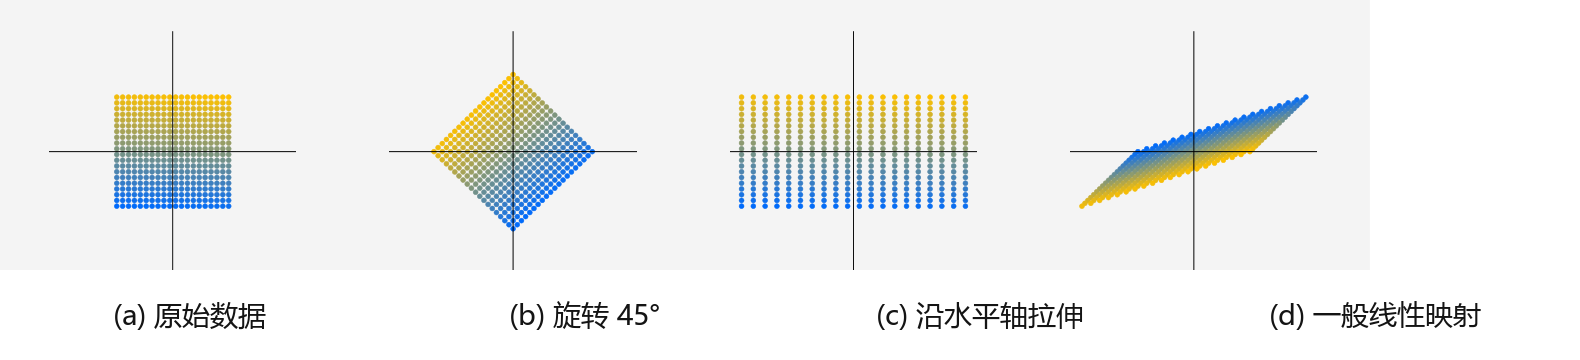
\includegraphics[width=0.92\textwidth,keepaspectratio]{docs/images/Figure2.10.png}
\caption*{\refstepcounter{figcounter}\label{fig:2-10}图~\thefigcounter 一组向量线性变换的三个示例。}
\end{figure}


\medskip\hrule\medskip

\section*{2.7.2 基变换}
\addcontentsline{toc}{subsection}{2.7.2 基变换}

在下文中，我们将更仔细地考察：如果我们改变 $ V $ 和 $ W $ 中的基，线性映射 $ \Phi : V \to W $ 的变换矩阵会如何变化。考虑 $ V $ 的两组有序基：

\begin{equation}
B = (\boldsymbol{b}_1, \ldots, \boldsymbol{b}_n), \quad \tilde{B} = (\tilde{\boldsymbol{b}}_1, \ldots, \tilde{\boldsymbol{b}}_n)
\tag{2.98}\label{eq:2-98}
\end{equation}

以及 $ W $ 的两组有序基：

\begin{equation}
C = (\boldsymbol{c}_1, \ldots, \boldsymbol{c}_m), \quad \tilde{C} = (\tilde{\boldsymbol{c}}_1, \ldots, \tilde{\boldsymbol{c}}_m)
\tag{2.99}\label{eq:2-99}
\end{equation}

此外，$ \boldsymbol{A}_\Phi \in \mathbb{R}^{m \times n} $ 是线性映射 $ \Phi : V \to W $ 关于基 $ B $ 与 $ C $ 的变换矩阵，而 $ \tilde{\boldsymbol{A}}_\Phi \in \mathbb{R}^{m \times n} $ 是对应于基 $ \tilde{B} $ 与 $ \tilde{C} $ 的变换矩阵。接下来我们将研究 $ \boldsymbol{A}_\Phi $ 与 $ \tilde{\boldsymbol{A}}_\Phi $ 之间的联系，即当我们选择从 $ B, C $ 进行基变换到 $ \tilde{B}, \tilde{C} $ 时，能否/如何将 $ \boldsymbol{A}_\Phi $ 转化为 $ \tilde{\boldsymbol{A}}_\Phi $。

\emph{备注} 。这实际上相当于我们获得了恒等映射 $ \operatorname{id}_V $ 的不同坐标表示。在图~\ref{fig:2-9} 的背景下，这意味着在不改变向量 $ \boldsymbol{x} $ 的前提下，将关于 $ (\boldsymbol{e}_1, \boldsymbol{e}_2) $ 的坐标映射到关于 $ (\boldsymbol{b}_1, \boldsymbol{b}_2) $ 的坐标。通过改变基以及相应地改变向量的表示，变换矩阵在这一新基下可以呈现出一种极其简单的形式（例如对角矩阵），从而大幅简化计算。

\begin{notebox}
\textbf{例 2.23（基变换）}
\end{notebox}

\begin{notebox}
考虑关于 $ \mathbb{R}^2 $ 标准基的变换矩阵：

\begin{equation}
\boldsymbol{A} = \begin{bmatrix} 2 & 1 \\ 1 & 2 \end{bmatrix}
\tag{2.100}\label{eq:2-100}
\end{equation}

如果我们定义一组新的基：

\begin{equation}
B = \left( \begin{bmatrix} 1 \\ 1 \end{bmatrix}, \begin{bmatrix} 1 \\ -1 \end{bmatrix} \right)
\tag{2.101}\label{eq:2-101}
\end{equation}

我们将获得关于新基 $ B $ 的对角变换矩阵：

\begin{equation}
\tilde{\boldsymbol{A}} = \begin{bmatrix} 3 & 0 \\ 0 & 1 \end{bmatrix}
\tag{2.102}\label{eq:2-102}
\end{equation}

它显然比 $ \boldsymbol{A} $ 更容易进行分析与运算。
\end{notebox}

下面，我们将研究将关于一组基的坐标向量转换为关于另一组基的坐标向量的映射。我们首先陈述核心结论，随后给出解释与证明。

\textbf{定理 2.20}（基变换）。对于线性映射 $ \Phi : V \to W $、$ V $ 的有序基：

\begin{equation}
B = (\boldsymbol{b}_1, \ldots, \boldsymbol{b}_n), \quad \tilde{B} = (\tilde{\boldsymbol{b}}_1, \ldots, \tilde{\boldsymbol{b}}_n)
\tag{2.103}\label{eq:2-103}
\end{equation}

$ W $ 的有序基：

\begin{equation}
C = (\boldsymbol{c}_1, \ldots, \boldsymbol{c}_m), \quad \tilde{C} = (\tilde{\boldsymbol{c}}_1, \ldots, \tilde{\boldsymbol{c}}_m)
\tag{2.104}\label{eq:2-104}
\end{equation}

以及 $ \Phi $ 关于 $ B $ 与 $ C $ 的变换矩阵 $ \boldsymbol{A}_\Phi $，其关于新基 $ \tilde{B} $ 与 $ \tilde{C} $ 对应的变换矩阵 $ \tilde{\boldsymbol{A}}_\Phi $ 为：

\begin{equation}
\tilde{\boldsymbol{A}}_\Phi = \boldsymbol{T}^{-1} \boldsymbol{A}_\Phi \boldsymbol{S}
\tag{2.105}\label{eq:2-105}
\end{equation}

这里，$ \boldsymbol{S} \in \mathbb{R}^{n \times n} $ 是将关于 $ \tilde{B} $ 的坐标映射到关于 $ B $ 的坐标的恒等映射 $ \operatorname{id}_V $ 的变换矩阵；$ \boldsymbol{T} \in \mathbb{R}^{m \times m} $ 是将关于 $ \tilde{C} $ 的坐标映射到关于 $ C $ 的坐标的恒等映射 $ \operatorname{id}_W $ 的变换矩阵。

\textbf{证明}：遵循 Drumm 和 Weil (2001) 的思路，我们可以将 $ V $ 的新基 $ \tilde{B} $ 中的向量写成原基 $ B $ 的基向量的线性组合：

\begin{equation}
\tilde{\boldsymbol{b}}_j = s_{1j}\boldsymbol{b}_1 + \cdots + s_{nj}\boldsymbol{b}_n = \sum_{i=1}^n s_{ij}\boldsymbol{b}_i, \quad j = 1, \ldots, n
\tag{2.106}\label{eq:2-106}
\end{equation}

类似地，我们将 $ W $ 的新基向量 $ \tilde{C} $ 写成原基向量 $ C $ 的线性组合：

\begin{equation}
\tilde{\boldsymbol{c}}_k = t_{1k}\boldsymbol{c}_1 + \cdots + t_{mk}\boldsymbol{c}_m = \sum_{l=1}^m t_{lk}\boldsymbol{c}_l, \quad k = 1, \ldots, m
\tag{2.107}\label{eq:2-107}
\end{equation}

我们将 $ \boldsymbol{S} = ((s_{ij})) \in \mathbb{R}^{n \times n} $ 定义为将关于 $ \tilde{B} $ 的坐标映射到关于 $ B $ 的坐标的变换矩阵，将 $ \boldsymbol{T} = ((t_{lk})) \in \mathbb{R}^{m \times m} $ 定义为将关于 $ \tilde{C} $ 的坐标映射到关于 $ C $ 的坐标的变换矩阵。具体而言，$ \boldsymbol{S} $ 的第 $ j $ 列是 $ \tilde{\boldsymbol{b}}_j $ 关于 $ B $ 的坐标表示，而 $ \boldsymbol{T} $ 的第 $ k $ 列是 $ \tilde{\boldsymbol{c}}_k $ 关于 $ C $ 的坐标表示。请注意，$ \boldsymbol{S} $ 和 $ \boldsymbol{T} $ 都是正则矩阵（可逆方阵）。

我们将从两个视角来考察 $ \Phi(\tilde{\boldsymbol{b}}_j) $。

首先，根据映射 $ \Phi $ 在新基下的表示，对所有 $ j = 1, \ldots, n $ 有：

\begin{equation}
\begin{adjustbox}{max width=\linewidth}
\Phi(\tilde{\boldsymbol{b}}_j) = \sum_{k=1}^m \tilde{a}_{kj} \tilde{\boldsymbol{c}}_k = \sum_{k=1}^m \tilde{a}_{kj} \sum_{l=1}^m t_{lk}\boldsymbol{c}_l = \sum_{l=1}^m \left( \sum_{k=1}^m t_{lk} \tilde{a}_{kj} \right) \boldsymbol{c}_l
\end{adjustbox}
\tag{2.108}\label{eq:2-108}
\end{equation}

这里我们首先将新基向量 $ \tilde{\boldsymbol{c}}_k \in W $ 展开为原基向量 $ \boldsymbol{c}_l \in W $ 的线性组合，然后交换了求和顺序。

另一种视角，当我们将 $ \tilde{\boldsymbol{b}}_j \in V $ 展开为 $ \boldsymbol{b}_i \in V $ 的线性组合时，由 $ \Phi $ 的线性性质可得：

\begin{equation}
\Phi(\tilde{\boldsymbol{b}}_j) = \Phi\left( \sum_{i=1}^n s_{ij}\boldsymbol{b}_i \right) = \sum_{i=1}^n s_{ij} \Phi(\boldsymbol{b}_i) = \sum_{i=1}^n s_{ij} \sum_{l=1}^m a_{li}\boldsymbol{c}_l
\tag{2.109a}\label{eq:2-109a}
\end{equation}

\begin{equation}
= \sum_{l=1}^m \left( \sum_{i=1}^n a_{li}s_{ij} \right) \boldsymbol{c}_l, \quad j = 1, \ldots, n
\tag{2.109b}\label{eq:2-109b}
\end{equation}

对比 (2.108) 与 (2.109b)，由基展开的唯一性可知，对所有 $ j = 1, \ldots, n $ 和 $ l = 1, \ldots, m $ 均有：

\begin{equation}
\sum_{k=1}^m t_{lk} \tilde{a}_{kj} = \sum_{i=1}^n a_{li} s_{ij}
\tag{2.110}\label{eq:2-110}
\end{equation}

写成矩阵乘法形式即为：

\begin{equation}
\boldsymbol{T} \tilde{\boldsymbol{A}}_\Phi = \boldsymbol{A}_\Phi \boldsymbol{S} \in \mathbb{R}^{m \times n}
\tag{2.111}\label{eq:2-111}
\end{equation}

两边左乘 $ \boldsymbol{T}^{-1} $，即得到：

\begin{equation}
\tilde{\boldsymbol{A}}_\Phi = \boldsymbol{T}^{-1} \boldsymbol{A}_\Phi \boldsymbol{S}
\tag{2.112}\label{eq:2-112}
\end{equation}

这便完成了定理 2.20 的证明。

定理 2.20 说明，当 $ V $ 经历基变换（$ B $ 替换为 $ \tilde{B} $）且 $ W $ 经历基变换（$ C $ 替换为 $ \tilde{C} $）时，线性映射 $ \Phi : V \to W $ 的变换矩阵 $ \boldsymbol{A}_\Phi $ 将被替换为一个等价矩阵 $ \tilde{\boldsymbol{A}}_\Phi $：

\begin{equation}
\tilde{\boldsymbol{A}}_\Phi = \boldsymbol{T}^{-1} \boldsymbol{A}_\Phi \boldsymbol{S}
\tag{2.113}\label{eq:2-113}
\end{equation}

图~\ref{fig:2-11} 阐明了这一对应关系：考虑同态 $ \Phi : V \to W $ 以及 $ V $ 的有序基 $ B, \tilde{B} $ 和 $ W $ 的有序基 $ C, \tilde{C} $。映射 $ \Phi_{CB} $ 是 $ \Phi $ 的一个具体实例化，它将 $ B $ 的基向量映射为 $ C $ 的基向量的线性组合。假定我们已知 $ \Phi_{CB} $ 关于有序基 $ B, C $ 的变换矩阵 $ \boldsymbol{A}_\Phi $。当我们进行基变换时，我们可以通过以下三步确定对应的变换矩阵 $ \tilde{\boldsymbol{A}}_\Phi $：

\begin{enumerate}
\item 首先求出将关于新基 $ \tilde{B} $ 的坐标映射到关于“旧”基 $ B $ 的坐标的线性映射 $ \Psi_{B\tilde{B}} : V \to V $ 的矩阵表示 $ \boldsymbol{S} $；
\item 随后使用 $ \Phi_{CB} : V \to W $ 的变换矩阵 $ \boldsymbol{A}_\Phi $ 将这些坐标映射到关于 $ W $ 中基 $ C $ 的坐标；
\item 最后使用线性映射 $ \Xi_{\tilde{C}C} : W \to W $ 将关于 $ C $ 的坐标映射到关于 $ \tilde{C} $ 的坐标。
\end{enumerate}

因此，我们可以将新基下的线性映射 $ \Phi_{\tilde{C}\tilde{B}} $ 表示为包含旧基的映射的复合：

\begin{equation}
\Phi_{\tilde{C}\tilde{B}} = \Xi_{\tilde{C}C} \circ \Phi_{CB} \circ \Psi_{B\tilde{B}} = \Xi_{C\tilde{C}}^{-1} \circ \Phi_{CB} \circ \Psi_{B\tilde{B}}
\tag{2.114}\label{eq:2-114}
\end{equation}

具体而言，这里使用的 $ \Psi_{B\tilde{B}} = \operatorname{id}_V $ 与 $ \Xi_{C\tilde{C}} = \operatorname{id}_W $ 就是恒等映射，它们将向量映射到自身，但对应于不同的基表示。


\begin{figure}[H]
\centering
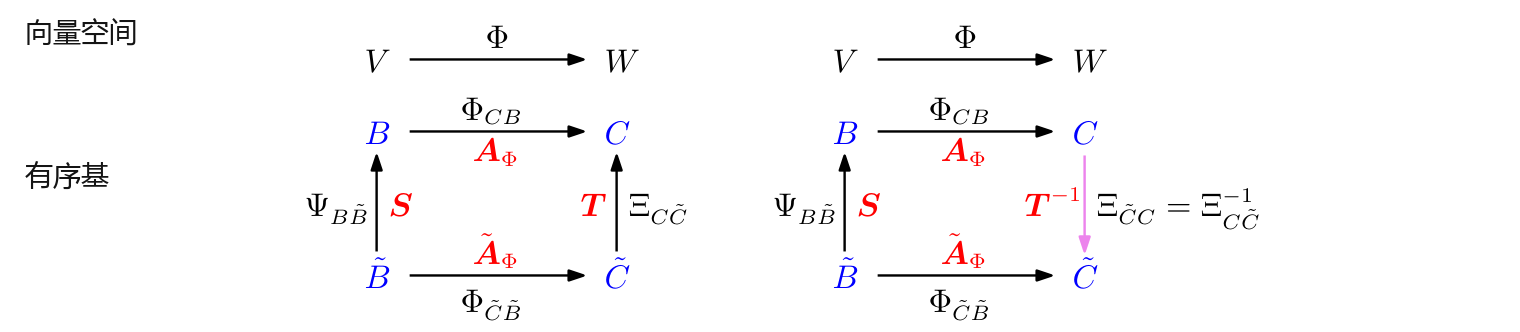
\includegraphics[width=0.92\textwidth,keepaspectratio]{docs/images/Figure2.11.png}
\caption*{\refstepcounter{figcounter}\label{fig:2-11}图~\thefigcounter 线性映射的基变换交换图解。}
\end{figure}


\textbf{定义 2.21}（等价）。如果存在正则矩阵 $ \boldsymbol{S} \in \mathbb{R}^{n \times n} $ 和 $ \boldsymbol{T} \in \mathbb{R}^{m \times m} $ 满足：

\begin{equation*}
\tilde{\boldsymbol{A}} = \boldsymbol{T}^{-1} \boldsymbol{A} \boldsymbol{S}
\end{equation*}

则称两个矩阵 $ \boldsymbol{A}, \tilde{\boldsymbol{A}} \in \mathbb{R}^{m \times n} $ 是 \emph{等价（equivalent）} 的。

\textbf{定义 2.22}（相似）。如果存在正则矩阵 $ \boldsymbol{S} \in \mathbb{R}^{n \times n} $ 满足：

\begin{equation*}
\tilde{\boldsymbol{A}} = \boldsymbol{S}^{-1} \boldsymbol{A} \boldsymbol{S}
\end{equation*}

则称两个方阵 $ \boldsymbol{A}, \tilde{\boldsymbol{A}} \in \mathbb{R}^{n \times n} $ 是 \emph{相似（similar）} 的。

\emph{备注} 。相似的矩阵必定是等价的。然而，等价的矩阵不一定是相似的。

\emph{备注} 。考虑向量空间 $ V, W, X $。从定理 2.17 后面的备注我们已知，对于线性映射 $ \Phi : V \to W $ 和 $ \Psi : W \to X $，复合映射 $ \Psi \circ \Phi : V \to X $ 也是线性的。若对应映射的变换矩阵分别为 $ \boldsymbol{A}_\Phi $ 和 $ \boldsymbol{A}_\Psi $，则整体复合映射的变换矩阵为 $ \boldsymbol{A}_{\Psi \circ \Phi} = \boldsymbol{A}_\Psi \boldsymbol{A}_\Phi $。

从复合映射的角度，我们可以非常直观地理解基变换：

\begin{itemize}
\item $ \boldsymbol{A}_\Phi $ 是线性映射 $ \Phi_{CB} : V \to W $ 关于基 $ B, C $ 的变换矩阵；
\item $ \tilde{\boldsymbol{A}}_\Phi $ 是线性映射 $ \Phi_{\tilde{C}\tilde{B}} : V \to W $ 关于基 $ \tilde{B}, \tilde{C} $ 的变换矩阵；
\item $ \boldsymbol{S} $ 是用 $ B $ 表示 $ \tilde{B} $ 的自同构 $ \Psi_{B\tilde{B}} : V \to V $ 的变换矩阵（通常 $ \Psi = \operatorname{id}_V $）；
\item $ \boldsymbol{T} $ 是用 $ C $ 表示 $ \tilde{C} $ 的自同构 $ \Xi_{C\tilde{C}} : W \to W $ 的变换矩阵（通常 $ \Xi = \operatorname{id}_W $）；
\end{itemize}

若非正式地仅从基的视角表示变换过程，则有 $ \boldsymbol{A}_\Phi : B \to C $、$ \tilde{\boldsymbol{A}}_\Phi : \tilde{B} \to \tilde{C} $、$ \boldsymbol{S} : \tilde{B} \to B $、$ \boldsymbol{T} : \tilde{C} \to C $ 以及 $ \boldsymbol{T}^{-1} : C \to \tilde{C} $，从而：

\begin{equation}
\tilde{B} \to \tilde{C} = \tilde{B} \to B \to C \to \tilde{C}
\tag{2.115}\label{eq:2-115}
\end{equation}

\begin{equation}
\tilde{\boldsymbol{A}}_\Phi = \boldsymbol{T}^{-1} \boldsymbol{A}_\Phi \boldsymbol{S}
\tag{2.116}\label{eq:2-116}
\end{equation}

请注意，(2.116) 中的运算执行顺序是从右往左的，因为向量相乘作用在右侧：

\begin{equation*}
\begin{adjustbox}{max width=\linewidth}
\boldsymbol{x} \mapsto \boldsymbol{S} \boldsymbol{x} \mapsto \boldsymbol{A}_\Phi(\boldsymbol{S} \boldsymbol{x}) \mapsto \boldsymbol{T}^{-1}\boldsymbol{A}_\Phi(\boldsymbol{S} \boldsymbol{x}) = \tilde{\boldsymbol{A}}_\Phi \boldsymbol{x}
\end{adjustbox}
\end{equation*}

。

\begin{notebox}
\textbf{例 2.24（基变换计算）}
\end{notebox}

\begin{notebox}
考虑一个线性映射 $ \Phi : \mathbb{R}^3 \to \mathbb{R}^4 $，其关于标准基 $ B $ 与 $ C $ 的变换矩阵为：

\begin{equation}
\boldsymbol{A}_\Phi = \begin{bmatrix} 1 & 2 & 0 \\ -1 & 1 & 3 \\ 3 & 7 & 1 \\ -1 & 2 & 4 \end{bmatrix}
\tag{2.117}\label{eq:2-117}
\end{equation}

其中标准基分别为：

\begin{equation}
\begin{adjustbox}{max width=\linewidth}
B = \left( \begin{bmatrix} 1 \\ 0 \\ 0 \end{bmatrix}, \begin{bmatrix} 0 \\ 1 \\ 0 \end{bmatrix}, \begin{bmatrix} 0 \\ 0 \\ 1 \end{bmatrix} \right), \quad C = \left( \begin{bmatrix} 1 \\ 0 \\ 0 \\ 0 \end{bmatrix}, \begin{bmatrix} 0 \\ 1 \\ 0 \\ 0 \end{bmatrix}, \begin{bmatrix} 0 \\ 0 \\ 1 \\ 0 \end{bmatrix}, \begin{bmatrix} 0 \\ 0 \\ 0 \\ 1 \end{bmatrix} \right)
\end{adjustbox}
\tag{2.118}\label{eq:2-118}
\end{equation}

我们寻求 $ \Phi $ 关于新基 $ \tilde{B} $ 与 $ \tilde{C} $ 的变换矩阵 $ \tilde{\boldsymbol{A}}_\Phi $：

\begin{equation}
\begin{adjustbox}{max width=\linewidth}
\tilde{B} = \left( \begin{bmatrix} 1 \\ 1 \\ 0 \end{bmatrix}, \begin{bmatrix} 0 \\ 1 \\ 1 \end{bmatrix}, \begin{bmatrix} 1 \\ 0 \\ 1 \end{bmatrix} \right), \quad \tilde{C} = \left( \begin{bmatrix} 1 \\ 1 \\ 0 \\ 0 \end{bmatrix}, \begin{bmatrix} 1 \\ 0 \\ 1 \\ 0 \end{bmatrix}, \begin{bmatrix} 0 \\ 1 \\ 1 \\ 0 \end{bmatrix}, \begin{bmatrix} 1 \\ 0 \\ 0 \\ 1 \end{bmatrix} \right)
\end{adjustbox}
\tag{2.119}\label{eq:2-119}
\end{equation}

此时：

\begin{equation}
\begin{adjustbox}{max width=\linewidth}
\boldsymbol{S} = \begin{bmatrix} 1 & 0 & 1 \\ 1 & 1 & 0 \\ 0 & 1 & 1 \end{bmatrix}, \quad \boldsymbol{T} = \begin{bmatrix} 1 & 1 & 0 & 1 \\ 1 & 0 & 1 & 0 \\ 0 & 1 & 1 & 0 \\ 0 & 0 & 0 & 1 \end{bmatrix}
\end{adjustbox}
\tag{2.120}\label{eq:2-120}
\end{equation}

其中 $ \boldsymbol{S} $ 的第 $ i $ 列是 $ \tilde{\boldsymbol{b}}_i $ 关于基 $ B $ 的坐标表示。由于 $ B $ 是标准基，这一坐标表示可直接读出。对于一般的非标准基 $ B $，我们需要求解线性方程组 $ \sum_{i=1}^3 \lambda_i \boldsymbol{b}_i = \tilde{\boldsymbol{b}}_j $ 来确定坐标。类似地，$ \boldsymbol{T} $ 的第 $ j $ 列是 $ \tilde{\boldsymbol{c}}_j $ 关于基 $ C $ 的坐标表示。
\end{notebox}

\begin{notebox}
因此，我们计算可得：

\begin{equation}
\begin{adjustbox}{max width=\linewidth}
\tilde{\boldsymbol{A}}_\Phi = \boldsymbol{T}^{-1} \boldsymbol{A}_\Phi \boldsymbol{S} = \frac{1}{2} \begin{bmatrix} 1 & 1 & -1 & -1 \\ 1 & -1 & 1 & -1 \\ -1 & 1 & 1 & 1 \\ 0 & 0 & 0 & 2 \end{bmatrix} \begin{bmatrix} 3 & 2 & 1 \\ 0 & 4 & 2 \\ 10 & 8 & 4 \\ 1 & 6 & 3 \end{bmatrix}
\end{adjustbox}
\tag{2.121a}\label{eq:2-121a}
\end{equation}

\begin{equation}
= \begin{bmatrix} -4 & -4 & -2 \\ 6 & 0 & 0 \\ 4 & 8 & 4 \\ 1 & 6 & 3 \end{bmatrix}
\tag{2.121b}\label{eq:2-121b}
\end{equation}
\end{notebox}

在第 4 章中，我们将利用基变换的概念来寻找一组特殊的基，使得自同态在该基下的变换矩阵具有特别简洁的对角形。在第 10 章中，我们将研究数据压缩问题，并寻找一组便利的基，以便在将数据投影到该基上时使压缩损失最小化。

\medskip\hrule\medskip

\section*{2.7.3 像与核}
\addcontentsline{toc}{subsection}{2.7.3 像与核}

线性映射的像与核是具有若干重要性质的向量子空间。在下文中，我们将对其进行更细致的刻画。

\textbf{定义 2.23}（像与核）。对于线性映射 $ \Phi : V \to W $，我们将 \emph{核（kernel）} （或 \emph{零空间（null space）} ）定义为：

\begin{equation}
\operatorname{ker}(\Phi) := \Phi^{-1}(\boldsymbol{0}_W) = \{\boldsymbol{v} \in V : \Phi(\boldsymbol{v}) = \boldsymbol{0}_W\}
\tag{2.122}\label{eq:2-122}
\end{equation}

并将 \emph{像（image）} （或 \emph{值域（range）} ）定义为：

\begin{equation}
\operatorname{Im}(\Phi) := \Phi(V) = \{\boldsymbol{w} \in W \mid \exists \boldsymbol{v} \in V : \Phi(\boldsymbol{v}) = \boldsymbol{w}\}
\tag{2.123}\label{eq:2-123}
\end{equation}

我们分别称 $ V $ 和 $ W $ 为 $ \Phi $ 的 \emph{定义域（domain）} 与 \emph{到达域（codomain）} 。

直观地说，核是 $ V $ 中所有被 $ \Phi $ 映射为零向量 $ \boldsymbol{0}_W \in W $ 的向量构成的集合。像是 $ W $ 中所有可以由 $ V $ 中向量通过 $ \Phi $ “到达”的向量集合。图~\ref{fig:2-12} 给出了示意图。


\begin{figure}[H]
\centering
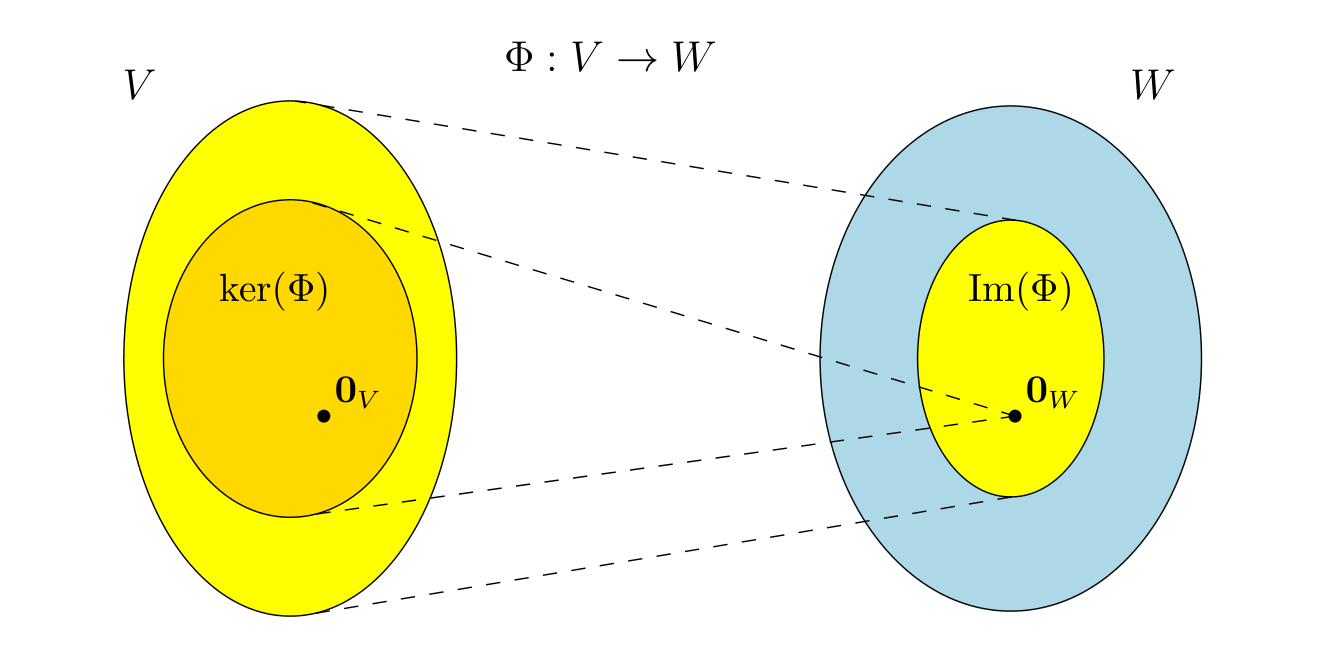
\includegraphics[width=0.92\textwidth,keepaspectratio]{docs/images/Figure2.12.png}
\caption*{\refstepcounter{figcounter}\label{fig:2-12}图~\thefigcounter 线性映射的核与像。}
\end{figure}


\emph{备注} 。考虑线性映射 $ \Phi : V \to W $（$ V, W $ 为向量空间）：

\begin{itemize}
\item 恒有 $ \Phi(\boldsymbol{0}_V) = \boldsymbol{0}_W $，因此 $ \boldsymbol{0}_V \in \operatorname{ker}(\Phi) $。特别地，零空间永非空集。
\item $ \operatorname{Im}(\Phi) \subseteq W $ 是 $ W $ 的子空间，且 $ \operatorname{ker}(\Phi) \subseteq V $ 是 $ V $ 的子空间。
\item $ \Phi $ 是单射（一对一映射）当且仅当 $ \operatorname{ker}(\Phi) = \{\boldsymbol{0}\} $。
\end{itemize}

\emph{备注} （零空间与列空间）。考虑矩阵 $ \boldsymbol{A} \in \mathbb{R}^{m \times n} $ 以及线性映射 $ \Phi : \mathbb{R}^n \to \mathbb{R}^m, \boldsymbol{x} \mapsto \boldsymbol{A} \boldsymbol{x} $：

\begin{itemize}
\item 设 $ \boldsymbol{A} = [\boldsymbol{a}_1, \ldots, \boldsymbol{a}_n] $（其中 $ \boldsymbol{a}_i $ 是 $ \boldsymbol{A} $ 的列），则： 即：像是由矩阵 $ \boldsymbol{A} $ 的列张成的空间，也称为 \emph{列空间（column space）} 。因此，列空间（像）是 $ \mathbb{R}^m $ 的子空间，其中 $ m $ 是矩阵的行数（高度）。
\end{itemize}
\begin{equation}
\operatorname{Im}(\Phi) = \{\boldsymbol{A} \boldsymbol{x} : \boldsymbol{x} \in \mathbb{R}^n\} = \left\{ \sum_{i=1}^n x_i \boldsymbol{a}_i : x_1, \ldots, x_n \in \mathbb{R} \right\}
\tag{2.124a}\label{eq:2-124a}
\end{equation}
\begin{equation}
= \operatorname{span}[\boldsymbol{a}_1, \ldots, \boldsymbol{a}_n] \subseteq \mathbb{R}^m
\tag{2.124b}\label{eq:2-124b}
\end{equation}
\begin{itemize}
\item $ \operatorname{rk}(\boldsymbol{A}) = \operatorname{dim}(\operatorname{Im}(\Phi)) $。
\item 核（零空间）$ \operatorname{ker}(\Phi) $ 是齐次线性方程组 $ \boldsymbol{A} \boldsymbol{x} = \boldsymbol{0} $ 的通解，捕获了 $ \mathbb{R}^n $ 中生成 $ \boldsymbol{0} \in \mathbb{R}^m $ 的所有可能线性组合。
\item 核是 $ \mathbb{R}^n $ 的子空间，其中 $ n $ 是矩阵的列数（宽度）。
\item 核关注列之间的相互关系，我们可以利用核来确定能否/如何将某一列表示为其余列的线性组合。
\end{itemize}

\begin{notebox}
\textbf{例 2.25（线性映射的像与核）}
\end{notebox}

\begin{notebox}
映射：

\begin{equation}
\begin{adjustbox}{max width=\linewidth}
\Phi : \mathbb{R}^4 \to \mathbb{R}^2, \quad \begin{bmatrix} x_1 \\ x_2 \\ x_3 \\ x_4 \end{bmatrix} \mapsto \begin{bmatrix} 1 & 2 & -1 & 0 \\ 1 & 0 & 0 & 1 \end{bmatrix} \begin{bmatrix} x_1 \\ x_2 \\ x_3 \\ x_4 \end{bmatrix} = \begin{bmatrix} x_1 + 2x_2 - x_3 \\ x_1 + x_4 \end{bmatrix}
\end{adjustbox}
\tag{2.125a}\label{eq:2-125a}
\end{equation}

\begin{equation}
= x_1 \begin{bmatrix} 1 \\ 1 \end{bmatrix} + x_2 \begin{bmatrix} 2 \\ 0 \end{bmatrix} + x_3 \begin{bmatrix} -1 \\ 0 \end{bmatrix} + x_4 \begin{bmatrix} 0 \\ 1 \end{bmatrix}
\tag{2.125b}\label{eq:2-125b}
\end{equation}

是线性的。为了确定 $ \operatorname{Im}(\Phi) $，我们可以取变换矩阵列向量的张成空间，得到：

\begin{equation}
\operatorname{Im}(\Phi) = \operatorname{span}\left[ \begin{bmatrix} 1 \\ 1 \end{bmatrix}, \begin{bmatrix} 2 \\ 0 \end{bmatrix}, \begin{bmatrix} -1 \\ 0 \end{bmatrix}, \begin{bmatrix} 0 \\ 1 \end{bmatrix} \right]
\tag{2.126}\label{eq:2-126}
\end{equation}

为了计算 $ \Phi $ 的核（零空间），我们需要求解 $ \boldsymbol{A} \boldsymbol{x} = \boldsymbol{0} $，即求解一个齐次方程组。为此，我们使用高斯消元法将 $ \boldsymbol{A} $ 化为简化行阶梯形矩阵：

\begin{equation}
\begin{adjustbox}{max width=\linewidth}
\begin{bmatrix} 1 & 2 & -1 & 0 \\ 1 & 0 & 0 & 1 \end{bmatrix} \leadsto \cdots \leadsto \begin{bmatrix} 1 & 0 & 0 & 1 \\ 0 & 1 & -\frac{1}{2} & -\frac{1}{2} \end{bmatrix}
\end{adjustbox}
\tag{2.127}\label{eq:2-127}
\end{equation}

该矩阵已呈简化行阶梯形，我们可以使用“减1技巧”直接读出核的一组基（参见第 2.3.3 节）。或者，我们可以将非主元列（第 3、4 列）表示为主元列（第 1、2 列）的线性组合：第三列 $ \boldsymbol{a}_3 $ 等于 $ -\frac{1}{2} \boldsymbol{a}_2 $，因此 $ \boldsymbol{0} = \boldsymbol{a}_3 + \frac{1}{2}\boldsymbol{a}_2 $；同理可得 $ \boldsymbol{a}_4 = \boldsymbol{a}_1 - \frac{1}{2}\boldsymbol{a}_2 $，即 $ \boldsymbol{0} = \boldsymbol{a}_1 - \frac{1}{2}\boldsymbol{a}_2 - \boldsymbol{a}_4 $。
\end{notebox}

\begin{notebox}
综合起来，我们得到核（零空间）为：

\begin{equation}
\operatorname{ker}(\Phi) = \operatorname{span}\left[ \begin{bmatrix} 0 \\ \frac{1}{2} \\ 1 \\ 0 \end{bmatrix}, \begin{bmatrix} -1 \\ \frac{1}{2} \\ 0 \\ 1 \end{bmatrix} \right]
\tag{2.128}\label{eq:2-128}
\end{equation}
\end{notebox}

\textbf{定理 2.24}（秩-零化度定理 / 线性映射基本定理）。对于向量空间 $ V, W $ 以及线性映射 $ \Phi : V \to W $，以下关系恒成立：

\begin{equation}
\operatorname{dim}(\operatorname{ker}(\Phi)) + \operatorname{dim}(\operatorname{Im}(\Phi)) = \operatorname{dim}(V)
\tag{2.129}\label{eq:2-129}
\end{equation}

秩-零化度定理（Rank-Nullity Theorem）也被称为 \emph{线性映射基本定理（fundamental theorem of linear mappings）} （Axler, 2015, 定理 3.22）。以下是定理 2.24 的直接推论：

\begin{itemize}
\item 如果 $ \operatorname{dim}(\operatorname{Im}(\Phi)) < \operatorname{dim}(V) $，则 $ \operatorname{ker}(\Phi) $ 是非平凡的，即核不仅包含零向量 $ \boldsymbol{0}_V $，且 $ \operatorname{dim}(\operatorname{ker}(\Phi)) \geqslant 1 $。
\item 如果 $ \boldsymbol{A}_\Phi $ 是 $ \Phi $ 关于某组有序基的变换矩阵，且 $ \operatorname{dim}(\operatorname{Im}(\Phi)) < \operatorname{dim}(V) $，则线性方程组 $ \boldsymbol{A}_\Phi \boldsymbol{x} = \boldsymbol{0} $ 拥有无穷多解。
\item 如果 $ \operatorname{dim}(V) = \operatorname{dim}(W) $，则由于 $ \operatorname{Im}(\Phi) \subseteq W $，以下三者彼此等价：
\begin{itemize}
\item $ \Phi $ 是单射；
\item $ \Phi $ 是满射；
\item $ \Phi $ 是双射。
\end{itemize}
\end{itemize}

\section*{2.8 仿射空间}
\addcontentsline{toc}{section}{2.8 仿射空间}
\label{sec:2.8}

在下文中，我们将仔细研究那些偏离原点的空间，即不再是向量子空间的空间。此外，我们还将简要讨论这些仿射空间之间的映射性质，这些性质类似于线性映射。

\emph{备注} 。在机器学习文献中，线性与仿射之间的区别有时并不严格分明，因此我们经常会看到将 \emph{仿射空间（affine spaces）} / \emph{仿射映射（affine mappings）} 称为 \emph{线性空间（linear spaces）} / \emph{线性映射（linear mappings）} 的情况。♦

\medskip\hrule\medskip

\section*{2.8.1 仿射子空间}
\addcontentsline{toc}{subsection}{2.8.1 仿射子空间}

\textbf{定义 2.25}（仿射子空间）。设 $ V $ 为向量空间，$ \boldsymbol{x}_0 \in V $，且 $ U \subseteq V $ 为其子空间。那么子集：

\begin{equation}
L = \boldsymbol{x}_0 + U := \{\boldsymbol{x}_0 + \boldsymbol{u} : \boldsymbol{u} \in U\}
\tag{2.130a}\label{eq:2-130a}
\end{equation}

\begin{equation}
= \{\boldsymbol{v} \in V \mid \exists \boldsymbol{u} \in U : \boldsymbol{v} = \boldsymbol{x}_0 + \boldsymbol{u}\} \subseteq V
\tag{2.130b}\label{eq:2-130b}
\end{equation}

称为 $ V $ 的 \emph{仿射子空间（affine subspace）} 或 \emph{线性流形（linear manifold）} 。$ U $ 称为 \emph{方向（direction）} 或 \emph{方向空间（direction space）} ，$ \boldsymbol{x}_0 $ 称为 \emph{支撑点（support point）} 。在第 12 章中，我们将此类子空间称为 \emph{超平面（hyperplane）} 。

注意：若 $ \boldsymbol{x}_0 \notin U $，则仿射子空间的定义排除了零向量 $ \boldsymbol{0} $。因此，当 $ \boldsymbol{x}_0 \notin U $ 时，仿射子空间不再是 $ V $ 的（线性）子空间（向量子空间）。

仿射子空间的示例包括 $ \mathbb{R}^3 $ 中（不一定）穿过原点的点、直线和平面。

\emph{备注} 。考虑向量空间 $ V $ 的两个仿射子空间 $ L = \boldsymbol{x}_0 + U $ 与 $ \tilde{L} = \tilde{\boldsymbol{x}}_0 + \tilde{U} $。那么，$ L \subseteq \tilde{L} $ 当且仅当 $ U \subseteq \tilde{U} $ 且 $ \boldsymbol{x}_0 - \tilde{\boldsymbol{x}}_0 \in \tilde{U} $。

仿射子空间通常通过参数来描述：考虑 $ V $ 的一个 $ k $ 维仿射空间 $ L = \boldsymbol{x}_0 + U $。如果 $ (\boldsymbol{b}_1, \ldots, \boldsymbol{b}_k) $ 是 $ U $ 的一组有序基，那么 $ L $ 中的每一个元素 $ \boldsymbol{x} $ 都可以唯一地表示为：

\begin{equation}
\boldsymbol{x} = \boldsymbol{x}_0 + \lambda_1 \boldsymbol{b}_1 + \cdots + \lambda_k \boldsymbol{b}_k
\tag{2.131}\label{eq:2-131}
\end{equation}

其中 $ \lambda_1, \ldots, \lambda_k \in \mathbb{R} $。该表示形式称为 $ L $ 的 \emph{参数方程（parametric equation）} ，其中 $ \boldsymbol{b}_1, \ldots, \boldsymbol{b}_k $ 称为 \emph{方向向量（directional vectors）} ，$ \lambda_1, \ldots, \lambda_k $ 称为 \emph{参数（parameters）} 。♦

\begin{notebox}
\textbf{例 2.26（仿射子空间）}
\end{notebox}

\begin{notebox}
$ \mathbb{R}^n $ 中的一维仿射子空间称为 \emph{直线（lines）} ，可以表示为 $ \boldsymbol{y} = \boldsymbol{x}_0 + \lambda \boldsymbol{x}_1 $，其中 $ \lambda \in \mathbb{R} $，且 $ U = \operatorname{span}[\boldsymbol{x}_1] \subseteq \mathbb{R}^n $ 是 $ \mathbb{R}^n $ 的一维子空间。这意味着直线由一个支撑点 $ \boldsymbol{x}_0 $ 和一个确定方向的向量 $ \boldsymbol{x}_1 $ 所决定。示意图参见图~\ref{fig:2-13}。
\end{notebox}

\begin{notebox}
$ \mathbb{R}^n $ 中的二维仿射子空间称为 \emph{平面（planes）} 。平面的参数方程为 $ \boldsymbol{y} = \boldsymbol{x}_0 + \lambda_1 \boldsymbol{x}_1 + \lambda_2 \boldsymbol{x}_2 $，其中 $ \lambda_1, \lambda_2 \in \mathbb{R} $ 且 $ U = \operatorname{span}[\boldsymbol{x}_1, \boldsymbol{x}_2] \subseteq \mathbb{R}^n $。这意味着平面由一个支撑点 $ \boldsymbol{x}_0 $ 和两个张成方向空间的线性无关向量 $ \boldsymbol{x}_1, \boldsymbol{x}_2 $ 所决定。
\end{notebox}

\begin{notebox}
在 $ \mathbb{R}^n $ 中，$ (n - 1) $ 维仿射子空间称为 \emph{超平面（hyperplanes）} ，其对应的参数方程为 $ \boldsymbol{y} = \boldsymbol{x}_0 + \sum_{i=1}^{n-1} \lambda_i \boldsymbol{x}_i $，其中 $ \boldsymbol{x}_1, \ldots, \boldsymbol{x}_{n-1} $ 构成 $ \mathbb{R}^n $ 的一个 $ (n - 1) $ 维子空间 $ U $ 的一组基。这意味着超平面由一个支撑点 $ \boldsymbol{x}_0 $ 和 $ (n - 1) $ 个张成方向空间的线性无关向量 $ \boldsymbol{x}_1, \ldots, \boldsymbol{x}_{n-1} $ 所决定。在 $ \mathbb{R}^2 $ 中，直线也是超平面；在 $ \mathbb{R}^3 $ 中，平面也是超平面。
\end{notebox}


\begin{figure}[H]
\centering
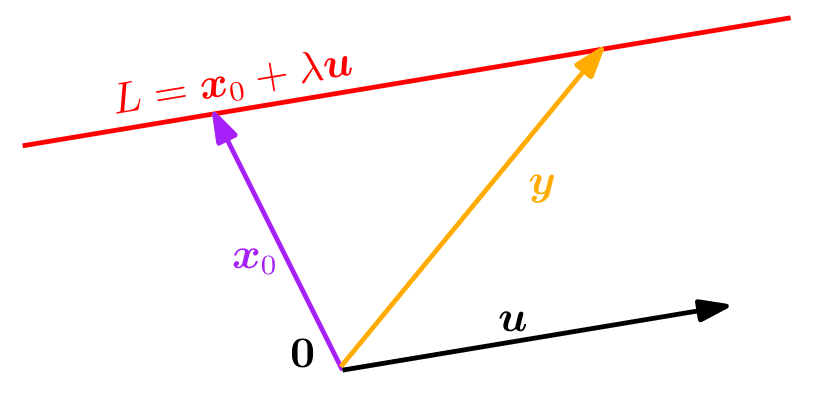
\includegraphics[width=0.92\textwidth,keepaspectratio]{docs/images/Figure2.13.png}
\caption*{\refstepcounter{figcounter}\label{fig:2-13}图~\thefigcounter 直线上的向量 y 位于以 x₀ 为支撑点、以 u 为方向的仿射子空间 L 中。}
\end{figure}


\emph{备注} （非齐次线性方程组与仿射子空间）。对于 $ \boldsymbol{A} \in \mathbb{R}^{m \times n} $ 以及 $ \boldsymbol{b} \in \mathbb{R}^m $，线性方程组 $ \boldsymbol{A} \boldsymbol{x} = \boldsymbol{b} $ 的解集要么是空集，要么是 $ \mathbb{R}^n $ 中维度为 $ n - \operatorname{rk}(\boldsymbol{A}) $ 的仿射子空间。特别地，线性方程 $ \lambda_1 x_1 + \cdots + \lambda_n x_n = b $（其中 $ (\lambda_1, \ldots, \lambda_n) \neq (0, \ldots, 0) $）的解是 $ \mathbb{R}^n $ 中的一个超平面。 在 $ \mathbb{R}^n $ 中，每一个 $ k $ 维仿射子空间都是某个非齐次线性方程组 $ \boldsymbol{A} \boldsymbol{x} = \boldsymbol{b} $ 的解，其中 $ \boldsymbol{A} \in \mathbb{R}^{m \times n} $，$ \boldsymbol{b} \in \mathbb{R}^m $ 且 $ \operatorname{rk}(\boldsymbol{A}) = n - k $。回想一下，齐次线性方程组 $ \boldsymbol{A} \boldsymbol{x} = \boldsymbol{0} $ 的解是一个向量子空间，我们也可以将其视为支撑点为 $ \boldsymbol{x}_0 = \boldsymbol{0} $ 的特殊仿射空间。♦

\medskip\hrule\medskip

\section*{2.8.2 仿射映射}
\addcontentsline{toc}{subsection}{2.8.2 仿射映射}

类似于我们在第 2.7 节中讨论的向量空间之间的线性映射，我们也可以定义两个仿射空间之间的仿射映射。线性映射与仿射映射密切相关。因此，我们从线性映射中获知的许多性质（例如线性映射的复合仍然是线性映射）对于仿射映射同样成立。

\textbf{定义 2.26}（仿射映射）。对于两个向量空间 $ V, W $、一个线性映射 $ \Phi : V \to W $ 以及 $ \boldsymbol{a} \in W $，映射：

\begin{equation}
\phi : V \to W
\tag{2.132}\label{eq:2-132}
\end{equation}

\begin{equation}
\boldsymbol{x} \mapsto \boldsymbol{a} + \Phi(\boldsymbol{x})
\tag{2.133}\label{eq:2-133}
\end{equation}

称为从 $ V $ 到 $ W $ 的 \emph{仿射映射（affine mapping）} 。向量 $ \boldsymbol{a} $ 称为 $ \phi $ 的 \emph{平移向量（translation vector）} 。

每一个仿射映射 $ \phi : V \to W $ 也是一个线性映射 $ \Phi : V \to W $ 与 $ W $ 上的一个 \emph{平移（translation）} $ \tau : W \to W $ 的复合，满足 $ \phi = \tau \circ \Phi $。映射 $ \Phi $ 与 $ \tau $ 是唯一确定的。

仿射映射 $ \phi : V \to W $ 与 $ \phi' : W \to X $ 的复合映射 $ \phi' \circ \phi $ 也是仿射的。

仿射映射保持几何结构不变。它们还保持维度与平行性（parallelism）。

\section*{2.9 延伸阅读}
\addcontentsline{toc}{section}{2.9 延伸阅读}
\label{sec:2.9}

学习线性代数的资源非常丰富，包括 Strang (2003)、Golan (2007)、Axler (2015) 以及 Liesen and Mehrmann (2015) 的教材。我们在本章引言中也提到了一些在线资源。在本书中我们仅介绍了高斯消元法，但求解线性方程组还有许多其他方法；若需更深入的讨论，请参阅 Stoer and Burlirsch (2002)、Golub and Van Loan (2012) 以及 Horn and Johnson (2013) 的数值线性代数教材。

在本书中，我们将线性代数的主题（例如向量、矩阵、线性无关、基）与向量空间的几何相关主题进行了区分。在第 3 章中，我们将引入 \emph{内积（inner product）} ，内积可诱导出 \emph{范数（norm）} 。这些概念使我们能够定义夹角、长度和距离，我们将利用它们来进行 \emph{正交投影（orthogonal projections）} 。事实证明，投影在许多机器学习算法中都起着关键作用，例如 \emph{线性回归（linear regression）} 和 \emph{主成分分析（principal component analysis）} ，我们将在第 9 章和第 10 章分别对它们进行介绍。

\chapter*{练习}
\addcontentsline{toc}{section}{练习}

\section*{练习 3.1}
\addcontentsline{toc}{subsection}{练习 3.1}

证明：对于所有 $ \boldsymbol{x} = [x_1, x_2]^\top \in \mathbb{R}^2 $ 和 $ \boldsymbol{y} = [y_1, y_2]^\top \in \mathbb{R}^2 $，由下式定义的 $ \langle\cdot, \cdot\rangle $：

\begin{equation*}
\langle\boldsymbol{x}, \boldsymbol{y}\rangle := x_1 y_1 - (x_1 y_2 + x_2 y_1) + 2(x_2 y_2)
\end{equation*}

是一个内积。

\medskip\hrule\medskip

\section*{练习 3.2}
\addcontentsline{toc}{subsection}{练习 3.2}

考虑 $ \mathbb{R}^2 $，其中对于 $ \mathbb{R}^2 $ 中的所有 $ \boldsymbol{x} $ 和 $ \boldsymbol{y} $，定义 $ \langle\cdot, \cdot\rangle $ 为：

\begin{equation*}
\langle\boldsymbol{x}, \boldsymbol{y}\rangle := \boldsymbol{x}^\top \underbrace{\begin{bmatrix} 2 & 0 \\ 1 & 2 \end{bmatrix}}_{=: \boldsymbol{A}} \boldsymbol{y}
\end{equation*}

$ \langle\cdot, \cdot\rangle $ 是一个内积吗？

\medskip\hrule\medskip

\section*{练习 3.3}
\addcontentsline{toc}{subsection}{练习 3.3}

计算

\begin{equation*}
\boldsymbol{x} = \begin{bmatrix} 1 \\ 2 \\ 3 \end{bmatrix}, \quad \boldsymbol{y} = \begin{bmatrix} -1 \\ -1 \\ 0 \end{bmatrix}
\end{equation*}

之间的距离，分别使用：

a. $ \langle\boldsymbol{x}, \boldsymbol{y}\rangle := \boldsymbol{x}^\top \boldsymbol{y} $ b. $ \langle\boldsymbol{x}, \boldsymbol{y}\rangle := \boldsymbol{x}^\top \boldsymbol{A} \boldsymbol{y} $，其中

\begin{equation*}
\boldsymbol{A} := \begin{bmatrix} 2 & 1 & 0 \\ 1 & 3 & -1 \\ 0 & -1 & 2 \end{bmatrix}
\end{equation*}

\medskip\hrule\medskip

\section*{练习 3.4}
\addcontentsline{toc}{subsection}{练习 3.4}

计算

\begin{equation*}
\boldsymbol{x} = \begin{bmatrix} 1 \\ 2 \end{bmatrix}, \quad \boldsymbol{y} = \begin{bmatrix} -1 \\ -1 \end{bmatrix}
\end{equation*}

之间的夹角，分别使用：

a. $ \langle\boldsymbol{x}, \boldsymbol{y}\rangle := \boldsymbol{x}^\top \boldsymbol{y} $ b. $ \langle\boldsymbol{x}, \boldsymbol{y}\rangle := \boldsymbol{x}^\top \boldsymbol{B} \boldsymbol{y} $，其中

\begin{equation*}
\boldsymbol{B} := \begin{bmatrix} 2 & 1 \\ 1 & 3 \end{bmatrix}
\end{equation*}

\medskip\hrule\medskip

\section*{练习 3.5}
\addcontentsline{toc}{subsection}{练习 3.5}

考虑带有点积的欧氏向量空间 $ \mathbb{R}^5 $。子空间 $ U \subseteq \mathbb{R}^5 $ 与向量 $ \boldsymbol{x} \in \mathbb{R}^5 $ 给定为：

\begin{equation*}
\begin{adjustbox}{max width=\linewidth}
U = \text{span}\left[ \begin{bmatrix} 0 \\ -1 \\ 2 \\ 0 \\ 2 \end{bmatrix}, \begin{bmatrix} 1 \\ -3 \\ 1 \\ -1 \\ 2 \end{bmatrix}, \begin{bmatrix} -3 \\ 4 \\ 1 \\ 2 \\ 1 \end{bmatrix}, \begin{bmatrix} -1 \\ -3 \\ 5 \\ 0 \\ 7 \end{bmatrix} \right], \quad \boldsymbol{x} = \begin{bmatrix} -1 \\ -9 \\ -1 \\ 4 \\ 1 \end{bmatrix}
\end{adjustbox}
\end{equation*}

a. 确定 $ \boldsymbol{x} $ 在 $ U $ 上的正交投影 $ \pi_U(\boldsymbol{x}) $。 b. 确定距离 $ d(\boldsymbol{x}, U) $。

\medskip\hrule\medskip

\section*{练习 3.6}
\addcontentsline{toc}{subsection}{练习 3.6}

考虑带有内积的 $ \mathbb{R}^3 $：

\begin{equation*}
\langle\boldsymbol{x}, \boldsymbol{y}\rangle := \boldsymbol{x}^\top \begin{bmatrix} 2 & 1 & 0 \\ 1 & 2 & -1 \\ 0 & -1 & 2 \end{bmatrix} \boldsymbol{y}
\end{equation*}

此外，定义 $ \boldsymbol{e}_1, \boldsymbol{e}_2, \boldsymbol{e}_3 $ 为 $ \mathbb{R}^3 $ 中的标准基。

a. 确定 $ \boldsymbol{e}_2 $ 在

\begin{equation*}
U = \text{span}[\boldsymbol{e}_1, \boldsymbol{e}_3]
\end{equation*}

上的正交投影 $ \pi_U(\boldsymbol{e}_2) $。 提示：正交性是通过该内积定义的。 b. 计算距离 $ d(\boldsymbol{e}_2, U) $。 c. 画出该场景示意图：标准基向量以及 $ \pi_U(\boldsymbol{e}_2) $。

\medskip\hrule\medskip

\section*{练习 3.7}
\addcontentsline{toc}{subsection}{练习 3.7}

设 $ V $ 为一个向量空间，$ \pi $ 为 $ V $ 上的一个自同态（endomorphism）。

a. 证明 $ \pi $ 是投影当且仅当 $ \text{id}_V - \pi $ 是投影，其中 $ \text{id}_V $ 是 $ V $ 上的恒等自同态。 b. 现在假设 $ \pi $ 是一个投影。计算 $ \text{Im}(\text{id}_V - \pi) $ 和 $ \text{ker}(\text{id}_V - \pi) $ 作为 $ \text{Im}(\pi) $ 和 $ \text{ker}(\pi) $ 的函数（即用 $ \text{Im}(\pi) $ 和 $ \text{ker}(\pi) $ 来表示它们）。

\medskip\hrule\medskip

\section*{练习 3.8}
\addcontentsline{toc}{subsection}{练习 3.8}

使用格拉姆-施密特方法（Gram-Schmidt method），将二维子空间 $ U \subseteq \mathbb{R}^3 $ 的一组基 $ B = (\boldsymbol{b}_1, \boldsymbol{b}_2) $ 化为 $ U $ 的一组标准正交基（ONB）$ C = (\boldsymbol{c}_1, \boldsymbol{c}_2) $，其中：

\begin{equation*}
\boldsymbol{b}_1 := \begin{bmatrix} 1 \\ 1 \\ 1 \end{bmatrix}, \quad \boldsymbol{b}_2 := \begin{bmatrix} -1 \\ 2 \\ 0 \end{bmatrix}
\end{equation*}

\medskip\hrule\medskip

\section*{练习 3.9}
\addcontentsline{toc}{subsection}{练习 3.9}

设 $ n \in \mathbb{N}^* $，并设 $ x_1, \ldots, x_n > 0 $ 为 $ n $ 个正实数，满足 $ x_1 + \cdots + x_n = 1 $。利用柯西-施瓦茨不等式证明：

a.

\begin{equation*}
\sum_{i=1}^n x_i^2 \geqslant \frac{1}{n}
\end{equation*}

b.

\begin{equation*}
\sum_{i=1}^n \frac{1}{x_i} \geqslant n^2
\end{equation*}

提示：考虑 $ \mathbb{R}^n $ 上的点积。然后选择特定的向量 $ \boldsymbol{x}, \boldsymbol{y} \in \mathbb{R}^n $ 并应用柯西-施瓦茨不等式。

\medskip\hrule\medskip

\section*{练习 3.10}
\addcontentsline{toc}{subsection}{练习 3.10}

将向量

\begin{equation*}
\boldsymbol{x}_1 := \begin{bmatrix} 2 \\ 3 \end{bmatrix}, \quad \boldsymbol{x}_2 := \begin{bmatrix} 0 \\ -1 \end{bmatrix}
\end{equation*}

旋转 $ 30^\circ $。

\chapter{3 解析几何}

在第 2 章中，我们在较为普遍且抽象的层面上研究了向量、向量空间和线性映射。在本章中，我们将为所有这些概念增添几何解释与几何直觉。特别地，我们将考察几何向量，并计算其长度、距离以及两个向量之间的夹角。为了实现这一点，我们为向量空间赋予一个 \emph{内积（inner product）} ，从而诱导出向量空间的几何结构。内积及其所对应的范数和度量刻画了相似性与距离的直观概念，我们将在第 12 章中利用这些概念来构建支持向量机。随后，我们将利用向量之间的长度和夹角概念来讨论正交投影，这将在第 10 章的主成分分析以及第 9 章通过极大似然估计进行回归时发挥核心作用。图~\ref{fig:3-1} 概述了本章各个概念之间的关系，以及它们与本书其他章节的联系。


\begin{figure}[H]
\centering
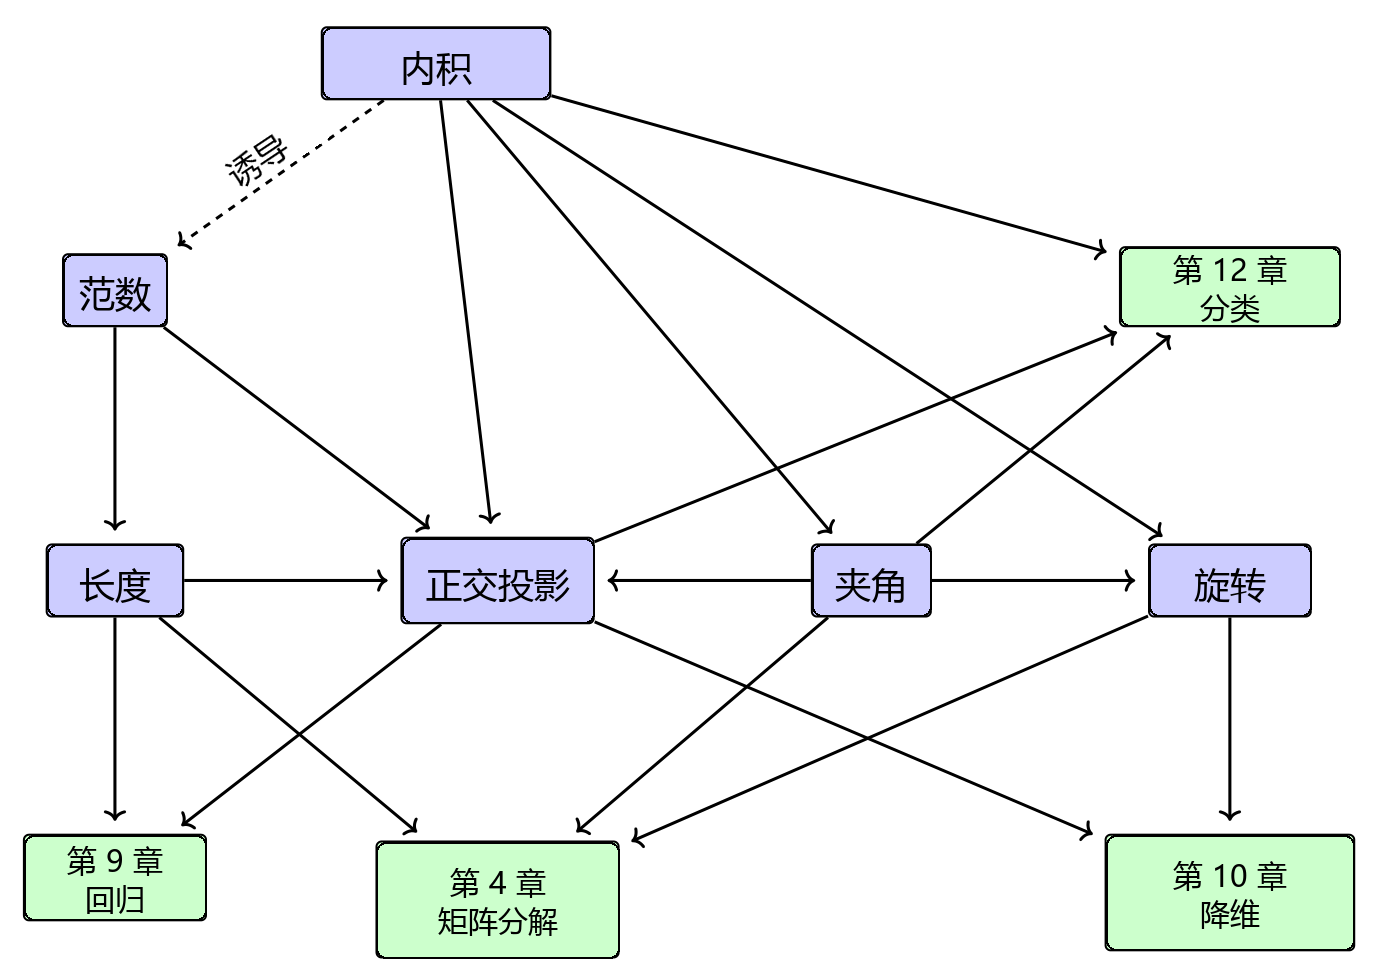
\includegraphics[width=0.92\textwidth,keepaspectratio]{docs/images/Figure3.1.png}
\caption*{\refstepcounter{figcounter}\label{fig:3-1}图~\thefigcounter 本章介绍的概念的思维导图，以及它们在本书其他部分中的应用场景。}
\end{figure}


\section*{3.1 范数}
\addcontentsline{toc}{section}{3.1 范数}
\label{sec:3.1}

当我们考虑几何向量（即从原点出发的有向线段）时，向量的长度在直观上就是该有向线段的“端点”到原点的距离。下面，我们将利用 \emph{范数（norm）} 的概念来讨论向量的长度。

\textbf{定义 3.1}（范数）。向量空间 $ V $ 上的 \emph{范数（norm）} 是一个函数：

\begin{equation}
\|\cdot\| : V \to \mathbb{R}
\tag{3.1}\label{eq:3-1}
\end{equation}

\begin{equation}
\boldsymbol{x} \mapsto \|\boldsymbol{x}\|
\tag{3.2}\label{eq:3-2}
\end{equation}

它为每个向量 $ \boldsymbol{x} $ 分配其长度 $ \|\boldsymbol{x}\| \in \mathbb{R} $，使得对于所有 $ \lambda \in \mathbb{R} $ 以及 $ \boldsymbol{x}, \boldsymbol{y} \in V $，满足以下性质：

\begin{itemize}
\item \emph{绝对齐次性（absolutely homogeneous）} ：$ \|\lambda \boldsymbol{x}\| = |\lambda| \|\boldsymbol{x}\| $
\item \emph{三角不等式（triangle inequality）} ：$ \|\boldsymbol{x} + \boldsymbol{y}\| \leqslant \|\boldsymbol{x}\| + \|\boldsymbol{y}\| $
\item \emph{正定性（positive definite）} ：$ \|\boldsymbol{x}\| \geqslant 0 $ 且 $ \|\boldsymbol{x}\| = 0 \iff \boldsymbol{x} = \boldsymbol{0} $
\end{itemize}


\begin{figure}[H]
\centering
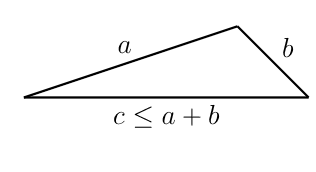
\includegraphics[width=0.92\textwidth,keepaspectratio]{docs/images/Figure3.2.png}
\caption*{\refstepcounter{figcounter}\label{fig:3-2}图~\thefigcounter 三角不等式。}
\end{figure}


从几何意义上讲，三角不等式表明对于任意三角形，任意两边长度之和必须大于或等于第三边的长度；参见图~\ref{fig:3-2} 的示意说明。

定义 3.1 是针对一般向量空间 $ V $（第 2.4 节）给出的，但在本书中，我们将主要考虑有限维向量空间 $ \mathbb{R}^n $。回想一下，对于向量 $ \boldsymbol{x} \in \mathbb{R}^n $，我们使用下标表示该向量的分量，即 $ x_i $ 是向量 $ \boldsymbol{x} $ 的第 $ i $ 个元素。

\begin{notebox}
\textbf{例 3.1（曼哈顿范数）}
\end{notebox}

\begin{notebox}
$ \mathbb{R}^n $ 上的 \emph{曼哈顿范数（Manhattan norm）} 对 $ \boldsymbol{x} \in \mathbb{R}^n $ 定义为：

\begin{equation}
\|\boldsymbol{x}\|_1 := \sum_{i=1}^n |x_i|
\tag{3.3}\label{eq:3-3}
\end{equation}

其中 $ |\cdot| $ 表示绝对值。图~\ref{fig:3-3} 左图显示了 $ \mathbb{R}^2 $ 中所有满足 $ \|\boldsymbol{x}\|_1 = 1 $ 的向量 $ \boldsymbol{x} $。曼哈顿范数也被称为 $ \ell_1 $ 范数（$ \ell_1 $ norm）。
\end{notebox}


\begin{figure}[H]
\centering
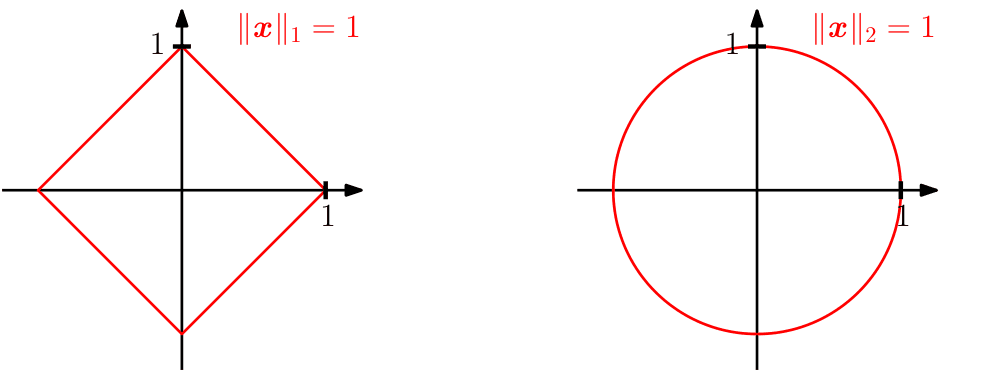
\includegraphics[width=0.92\textwidth,keepaspectratio]{docs/images/Figure3.3.png}
\caption*{\refstepcounter{figcounter}\label{fig:3-3}图~\thefigcounter 对于不同范数，红线表示范数为 1 的向量集合。左图：曼哈顿范数；右图：欧几里得距离。}
\end{figure}


\begin{notebox}
\textbf{例 3.2（欧几里得范数）}
\end{notebox}

\begin{notebox}
$ \boldsymbol{x} \in \mathbb{R}^n $ 的 \emph{欧几里得范数（Euclidean norm）} 定义为：

\begin{equation}
\|\boldsymbol{x}\|_2 := \sqrt{\sum_{i=1}^n x_i^2} = \sqrt{\boldsymbol{x}^\top \boldsymbol{x}}
\tag{3.4}\label{eq:3-4}
\end{equation}

它计算了 $ \boldsymbol{x} $ 到原点的 \emph{欧几里得距离（Euclidean distance）} 。图~\ref{fig:3-3} 右图显示了 $ \mathbb{R}^2 $ 中所有满足 $ \|\boldsymbol{x}\|_2 = 1 $ 的向量 $ \boldsymbol{x} $。欧几里得范数也被称为 $ \ell_2 $ 范数（$ \ell_2 $ norm）。
\end{notebox}

\emph{备注} 。在本书通篇中，若无特殊说明，我们将默认使用欧几里得范数 (3.4)。♦

\section*{3.2 内积}
\addcontentsline{toc}{section}{3.2 内积}
\label{sec:3.2}

内积允许我们引入直观的几何概念，例如向量的长度以及两个向量之间的夹角或距离。内积的一个主要目的是确定向量之间是否相互正交。

\section*{3.2.1 点积}
\addcontentsline{toc}{subsection}{3.2.1 点积}

我们可能已经熟悉一种特殊类型的内积，即 $ \mathbb{R}^n $ 中的 \emph{标量积（scalar product）} / \emph{点积（dot product）} ，其由下式给出：

\begin{equation}
\boldsymbol{x}^\top \boldsymbol{y} = \sum_{i=1}^n x_i y_i
\tag{3.5}\label{eq:3-5}
\end{equation}

在本书中，我们将这种特定的内积称为点积。然而，内积是具有特定性质的更一般的概念，我们现在就来介绍它们。

\section*{3.2.2 一般内积}
\addcontentsline{toc}{subsection}{3.2.2 一般内积}

回顾第 2.7 节中的线性映射，我们可以根据加法和与标量的乘法重新排列该映射。 \emph{双线性映射（bilinear mapping）} $ \Omega $ 是一个具有两个自变量的映射，并且它在每个自变量上都是线性的，也就是说，当我们考虑向量空间 $ V $ 时，对于所有 $ \boldsymbol{x}, \boldsymbol{y}, \boldsymbol{z} \in V $ 以及 $ \lambda, \psi \in \mathbb{R} $，均有：

\begin{equation}
\Omega(\lambda \boldsymbol{x} + \psi \boldsymbol{y}, \boldsymbol{z}) = \lambda \Omega(\boldsymbol{x}, \boldsymbol{z}) + \psi \Omega(\boldsymbol{y}, \boldsymbol{z})
\tag{3.6}\label{eq:3-6}
\end{equation}

\begin{equation}
\Omega(\boldsymbol{x}, \lambda \boldsymbol{y} + \psi \boldsymbol{z}) = \lambda \Omega(\boldsymbol{x}, \boldsymbol{y}) + \psi \Omega(\boldsymbol{x}, \boldsymbol{z})
\tag{3.7}\label{eq:3-7}
\end{equation}

这里，式~\eqref{eq:3-6} 表明 $ \Omega $ 在第一个自变量上是线性的，而式~\eqref{eq:3-7} 表明 $ \Omega $ 在第二个自变量上是线性的（亦见式~\eqref{eq:2-87}）。

\textbf{定义 3.2}。设 $ V $ 为向量空间，$ \Omega : V \times V \to \mathbb{R} $ 是一个将两个向量映射为一个实数的双线性映射。那么： 如果对所有 $ \boldsymbol{x}, \boldsymbol{y} \in V $ 均有 $ \Omega(\boldsymbol{x}, \boldsymbol{y}) = \Omega(\boldsymbol{y}, \boldsymbol{x}) $，即自变量的顺序无关紧要，则称 $ \Omega $ 是 \emph{对称的（symmetric）} 。 如果满足：

\begin{equation}
\forall \boldsymbol{x} \in V \setminus \{\boldsymbol{0}\} : \Omega(\boldsymbol{x}, \boldsymbol{x}) > 0, \quad \Omega(\boldsymbol{0}, \boldsymbol{0}) = 0
\tag{3.8}\label{eq:3-8}
\end{equation}

则称 $ \Omega $ 是 \emph{正定的（positive definite）} 。

\textbf{定义 3.3}。设 $ V $ 为向量空间，$ \Omega : V \times V \to \mathbb{R} $ 是一个将两个向量映射为一个实数的双线性映射。 正定且对称的双线性映射 $ \Omega : V \times V \to \mathbb{R} $ 称为 $ V $ 上的 \emph{内积（inner product）} 。我们通常写成 $ \langle \boldsymbol{x}, \boldsymbol{y} \rangle $ 而不是 $ \Omega(\boldsymbol{x}, \boldsymbol{y}) $。 二元组 $ (V, \langle \cdot, \cdot \rangle) $ 称为 \emph{内积空间（inner product space）} 或 \emph{（实）赋内积向量空间（(real) vector space with inner product）} 。如果我们使用式~\eqref{eq:3-5} 中定义的点积，则称 $ (V, \langle \cdot, \cdot \rangle) $ 为 \emph{欧几里得向量空间（Euclidean vector space）} 。 在本书中，我们将这些空间统称为内积空间。

\begin{notebox}
\textbf{例 3.3（非点积的内积）}
\end{notebox}

\begin{notebox}
考虑 $ V = \mathbb{R}^2 $。如果我们定义：

\begin{equation}
\langle \boldsymbol{x}, \boldsymbol{y} \rangle := x_1 y_1 - (x_1 y_2 + x_2 y_1) + 2 x_2 y_2
\tag{3.9}\label{eq:3-9}
\end{equation}

则 $ \langle \cdot, \cdot \rangle $ 是一个内积，但不同于点积。证明留作习题。
\end{notebox}

\section*{3.2.3 对称正定矩阵}
\addcontentsline{toc}{subsection}{3.2.3 对称正定矩阵}

对称正定矩阵在机器学习中起着重要作用，它们是通过内积来定义的。在第 4.3 节中，我们将在矩阵分解的背景下重新讨论对称正定矩阵。对称半正定矩阵的思想在核方法（第 12.4 节）的定义中至关重要。

考虑一个带有内积 $ \langle \cdot, \cdot \rangle : V \times V \to \mathbb{R} $（见定义 3.3）的 $ n $ 维向量空间 $ V $ 以及 $ V $ 的一组有序基 $ B = (\boldsymbol{b}_1, \ldots, \boldsymbol{b}_n) $。回顾第 2.6.1 节，任意向量 $ \boldsymbol{x}, \boldsymbol{y} \in V $ 都可以表示为基向量的线性组合，即对于适当的 $ \psi_i, \lambda_j \in \mathbb{R} $，有 $ \boldsymbol{x} = \sum_{i=1}^n \psi_i \boldsymbol{b}_i \in V $ 以及 $ \boldsymbol{y} = \sum_{j=1}^n \lambda_j \boldsymbol{b}_j \in V $。由于内积的双线性性质，对于所有 $ \boldsymbol{x}, \boldsymbol{y} \in V $，均有：

\begin{equation}
\begin{adjustbox}{max width=\linewidth}
\langle \boldsymbol{x}, \boldsymbol{y} \rangle = \left\langle \sum_{i=1}^n \psi_i \boldsymbol{b}_i, \sum_{j=1}^n \lambda_j \boldsymbol{b}_j \right\rangle = \sum_{i=1}^n \sum_{j=1}^n \psi_i \langle \boldsymbol{b}_i, \boldsymbol{b}_j \rangle \lambda_j = \hat{\boldsymbol{x}}^\top \boldsymbol{A} \hat{\boldsymbol{y}}
\end{adjustbox}
\tag{3.10}\label{eq:3-10}
\end{equation}

其中 $ A_{ij} := \langle \boldsymbol{b}_i, \boldsymbol{b}_j \rangle $，且 $ \hat{\boldsymbol{x}}, \hat{\boldsymbol{y}} $ 是 $ \boldsymbol{x} $ 和 $ \boldsymbol{y} $ 关于基 $ B $ 的坐标。这意味着内积 $ \langle \cdot, \cdot \rangle $ 由 $ \boldsymbol{A} $ 唯一确定。内积的对称性还意味着 $ \boldsymbol{A} $ 是对称的。此外，内积的正定性意味着：

\begin{equation}
\forall \boldsymbol{x} \in V \setminus \{\boldsymbol{0}\} : \boldsymbol{x}^\top \boldsymbol{A} \boldsymbol{x} > 0
\tag{3.11}\label{eq:3-11}
\end{equation}

\textbf{定义 3.4}（对称正定矩阵）。满足式~\eqref{eq:3-11} 的对称矩阵 $ \boldsymbol{A} \in \mathbb{R}^{n \times n} $ 称为 \emph{对称正定（symmetric, positive definite）} 矩阵，或简称为 \emph{正定（positive definite）} 矩阵。如果式~\eqref{eq:3-11} 中仅有 $ \geqslant $ 成立，则称 $ \boldsymbol{A} $ 为 \emph{对称半正定（symmetric, positive semidefinite）} 矩阵。

\begin{notebox}
\textbf{例 3.4（对称正定矩阵）}
\end{notebox}

\begin{notebox}
考虑矩阵：

\begin{equation}
\boldsymbol{A}_1 = \begin{bmatrix} 9 & 6 \\ 6 & 5 \end{bmatrix}, \quad \boldsymbol{A}_2 = \begin{bmatrix} 9 & 6 \\ 6 & 3 \end{bmatrix}
\tag{3.12}\label{eq:3-12}
\end{equation}

$ \boldsymbol{A}_1 $ 是正定的，因为它是对称的，并且对所有 $ \boldsymbol{x} \in V \setminus \{\boldsymbol{0}\} $ 都有：

\begin{equation}
\boldsymbol{x}^\top \boldsymbol{A}_1 \boldsymbol{x} = \begin{bmatrix} x_1 & x_2 \end{bmatrix} \begin{bmatrix} 9 & 6 \\ 6 & 5 \end{bmatrix} \begin{bmatrix} x_1 \\ x_2 \end{bmatrix}
\tag{3.13a}\label{eq:3-13a}
\end{equation}

\begin{equation}
= 9 x_1^2 + 12 x_1 x_2 + 5 x_2^2 = (3 x_1 + 2 x_2)^2 + x_2^2 > 0
\tag{3.13b}\label{eq:3-13b}
\end{equation}

相比之下，$ \boldsymbol{A}_2 $ 是对称的但不是正定的，因为 $ \boldsymbol{x}^\top \boldsymbol{A}_2 \boldsymbol{x} = 9 x_1^2 + 12 x_1 x_2 + 3 x_2^2 = (3 x_1 + 2 x_2)^2 - x_2^2 $ 可以小于 0，例如取 $ \boldsymbol{x} = [2, -3]^\top $。
\end{notebox}

如果 $ \boldsymbol{A} \in \mathbb{R}^{n \times n} $ 是对称正定的，则：

\begin{equation}
\langle \boldsymbol{x}, \boldsymbol{y} \rangle = \hat{\boldsymbol{x}}^\top \boldsymbol{A} \hat{\boldsymbol{y}}
\tag{3.14}\label{eq:3-14}
\end{equation}

定义了关于有序基 $ B $ 的一个内积，其中 $ \hat{\boldsymbol{x}} $ 和 $ \hat{\boldsymbol{y}} $ 是 $ \boldsymbol{x}, \boldsymbol{y} \in V $ 关于 $ B $ 的坐标表示。

\textbf{定理 3.5}。对于实值有限维向量空间 $ V $ 和 $ V $ 的一组有序基 $ B $，$ \langle \cdot, \cdot \rangle : V \times V \to \mathbb{R} $ 是内积当且仅当存在一个对称正定矩阵 $ \boldsymbol{A} \in \mathbb{R}^{n \times n} $ 满足：

\begin{equation}
\langle \boldsymbol{x}, \boldsymbol{y} \rangle = \hat{\boldsymbol{x}}^\top \boldsymbol{A} \hat{\boldsymbol{y}}
\tag{3.15}\label{eq:3-15}
\end{equation}

如果 $ \boldsymbol{A} \in \mathbb{R}^{n \times n} $ 是对称正定的，则具有以下性质：

\begin{itemize}
\item $ \boldsymbol{A} $ 的零空间（核）仅由 $ \boldsymbol{0} $ 组成，因为对所有 $ \boldsymbol{x} \neq \boldsymbol{0} $ 都有 $ \boldsymbol{x}^\top \boldsymbol{A} \boldsymbol{x} > 0 $。这意味着如果 $ \boldsymbol{x} \neq \boldsymbol{0} $，则 $ \boldsymbol{A} \boldsymbol{x} \neq \boldsymbol{0} $。
\item $ \boldsymbol{A} $ 的对角线元素 $ a_{ii} $ 均为正数，因为 $ a_{ii} = \boldsymbol{e}_i^\top \boldsymbol{A} \boldsymbol{e}_i > 0 $，其中 $ \boldsymbol{e}_i $ 是 $ \mathbb{R}^n $ 中标准基的第 $ i $ 个基向量。
\end{itemize}

\section*{3.3 长度与距离}
\addcontentsline{toc}{section}{3.3 长度与距离}
\label{sec:3.3}

在第 3.1 节中，我们已经讨论了可用于计算向量长度的范数。内积与范数之间密切相关，因为任何内积都会以自然的方式诱导出范数：

\begin{equation}
\|\boldsymbol{x}\| := \sqrt{\langle \boldsymbol{x}, \boldsymbol{x} \rangle}
\tag{3.16}\label{eq:3-16}
\end{equation}

从而使我们能够使用内积来计算向量的长度。然而，并非每个范数都是由内积诱导的。曼哈顿范数 (3.3) 就是一个没有对应内积的范数示例。在下文中，我们将重点关注由内积诱导的范数，并引入几何概念，如长度、距离和夹角。

\emph{备注} （柯西-施瓦茨不等式）。对于内积向量空间 $ (V, \langle \cdot, \cdot \rangle) $，诱导范数 $ \|\cdot\| $ 满足 \emph{柯西-施瓦茨不等式（Cauchy-Schwarz inequality）} ：

\begin{equation}
|\langle \boldsymbol{x}, \boldsymbol{y} \rangle| \leqslant \|\boldsymbol{x}\| \|\boldsymbol{y}\|
\tag{3.17}\label{eq:3-17}
\end{equation}

♦

\begin{notebox}
\textbf{例 3.5（使用内积计算向量的长度）}
\end{notebox}

\begin{notebox}
在几何学中，我们通常对向量的长度感兴趣。现在我们可以使用内积通过式~\eqref{eq:3-16} 来计算它们。取 $ \boldsymbol{x} = [1, 1]^\top \in \mathbb{R}^2 $。如果我们使用点积作为内积，根据式~\eqref{eq:3-16}，我们得到 $ \boldsymbol{x} $ 的长度为：

\begin{equation}
\|\boldsymbol{x}\| = \sqrt{\boldsymbol{x}^\top \boldsymbol{x}} = \sqrt{1^2 + 1^2} = \sqrt{2}
\tag{3.18}\label{eq:3-18}
\end{equation}

现在让我们选择另一个不同的内积：

\begin{equation}
\langle \boldsymbol{x}, \boldsymbol{y} \rangle := \boldsymbol{x}^\top \begin{bmatrix} 1 & -\frac{1}{2} \\ -\frac{1}{2} & 1 \end{bmatrix} \boldsymbol{y} = x_1 y_1 - \frac{1}{2}(x_1 y_2 + x_2 y_1) + x_2 y_2
\tag{3.19}\label{eq:3-19}
\end{equation}

如果我们计算一个向量的范数，当 $ x_1 $ 和 $ x_2 $ 同号（且 $ x_1 x_2 > 0 $）时，该内积返回的值小于点积；否则，它返回的值大于点积。在这个内积下，我们得到：

\begin{equation}
\langle \boldsymbol{x}, \boldsymbol{x} \rangle = x_1^2 - x_1 x_2 + x_2^2 = 1 - 1 + 1 = 1 \implies \|\boldsymbol{x}\| = \sqrt{1} = 1
\tag{3.20}\label{eq:3-20}
\end{equation}

因此在这个内积下，$ \boldsymbol{x} $ 比在点积下更“短”。
\end{notebox}

\textbf{定义 3.6}（距离与度量）。考虑一个内积空间 $ (V, \langle \cdot, \cdot \rangle) $。那么对于 $ \boldsymbol{x}, \boldsymbol{y} \in V $，

\begin{equation}
d(\boldsymbol{x}, \boldsymbol{y}) := \|\boldsymbol{x} - \boldsymbol{y}\| = \sqrt{\langle \boldsymbol{x} - \boldsymbol{y}, \boldsymbol{x} - \boldsymbol{y} \rangle}
\tag{3.21}\label{eq:3-21}
\end{equation}

称为 $ \boldsymbol{x} $ 与 $ \boldsymbol{y} $ 之间的 \emph{距离（distance）} 。如果我们使用点积作为内积，则该距离称为 \emph{欧几里得距离（Euclidean distance）} 。 映射：

\begin{equation}
d : V \times V \to \mathbb{R}
\tag{3.22}\label{eq:3-22}
\end{equation}

\begin{equation}
(\boldsymbol{x}, \boldsymbol{y}) \mapsto d(\boldsymbol{x}, \boldsymbol{y})
\tag{3.23}\label{eq:3-23}
\end{equation}

称为 \emph{度量（metric）} 。

\emph{备注} 。与向量的长度类似，向量之间的距离并不一定需要内积：范数就足够了。如果我们使用的是由内积诱导的范数，则距离可能会随着内积的选择而变化。♦

度量 $ d $ 满足以下性质：

\begin{enumerate}
\item $ d $ 是 \emph{正定的（positive definite）} ，即对所有 $ \boldsymbol{x}, \boldsymbol{y} \in V $，有 $ d(\boldsymbol{x}, \boldsymbol{y}) \geqslant 0 $，且 $ d(\boldsymbol{x}, \boldsymbol{y}) = 0 \iff \boldsymbol{x} = \boldsymbol{y} $。
\item $ d $ 是 \emph{对称的（symmetric）} ，即对所有 $ \boldsymbol{x}, \boldsymbol{y} \in V $，有 $ d(\boldsymbol{x}, \boldsymbol{y}) = d(\boldsymbol{y}, \boldsymbol{x}) $。
\item \emph{三角不等式（triangle inequality）} ：对所有 $ \boldsymbol{x}, \boldsymbol{y}, \boldsymbol{z} \in V $，有 $ d(\boldsymbol{x}, \boldsymbol{z}) \leqslant d(\boldsymbol{x}, \boldsymbol{y}) + d(\boldsymbol{y}, \boldsymbol{z}) $。
\end{enumerate}

\emph{备注} 。乍一看，内积和度量的性质列表非常相似。然而，通过对比定义 3.3 与定义 3.6，我们发现 $ \langle \boldsymbol{x}, \boldsymbol{y} \rangle $ 与 $ d(\boldsymbol{x}, \boldsymbol{y}) $ 的变化方向相反。非常相似的 $ \boldsymbol{x} $ 和 $ \boldsymbol{y} $ 会使内积取较大的值，而使度量取较小的值。♦

\section*{3.4 夹角与正交性}
\addcontentsline{toc}{section}{3.4 夹角与正交性}
\label{sec:3.4}

内积除了能够定义向量的长度以及两个向量之间的距离外，还可以通过定义两个向量之间的夹角 $ \omega $ 来刻画向量空间的几何性质。我们利用柯西-施瓦茨不等式~\eqref{eq:3-17} 来定义内积空间中两个向量 $ \boldsymbol{x}, \boldsymbol{y} $ 之间的夹角 $ \omega $，这一概念与我们在 $ \mathbb{R}^2 $ 和 $ \mathbb{R}^3 $ 中的直觉完全一致。假设 $ \boldsymbol{x} \neq \boldsymbol{0}, \boldsymbol{y} \neq \boldsymbol{0} $。则有：

\begin{equation}
-1 \leqslant \frac{\langle \boldsymbol{x}, \boldsymbol{y} \rangle}{\|\boldsymbol{x}\| \|\boldsymbol{y}\|} \leqslant 1
\tag{3.24}\label{eq:3-24}
\end{equation}

因此，存在唯一的 $ \omega \in [0, \pi] $（如图~\ref{fig:3-4} 所示），满足：

\begin{equation}
\cos \omega = \frac{\langle \boldsymbol{x}, \boldsymbol{y} \rangle}{\|\boldsymbol{x}\| \|\boldsymbol{y}\|}
\tag{3.25}\label{eq:3-25}
\end{equation}

数值 $ \omega $ 即为向量 $ \boldsymbol{x} $ 与 $ \boldsymbol{y} $ 之间的 \emph{夹角（angle）} 。直观上，两个向量之间的夹角反映了它们的方向有多相似。例如，使用点积时，$ \boldsymbol{x} $ 与 $ \boldsymbol{y} = 4\boldsymbol{x} $（即 $ \boldsymbol{y} $ 是 $ \boldsymbol{x} $ 的缩放版本）之间的夹角为 0：它们的方向是相同的。


\begin{figure}[H]
\centering
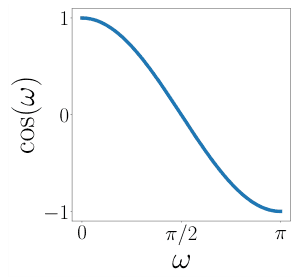
\includegraphics[width=0.92\textwidth,keepaspectratio]{docs/images/Figure3.4.png}
\caption*{\refstepcounter{figcounter}\label{fig:3-4}图~\thefigcounter 当限制在 [0, π] 上时，f(ω) = cos(ω) 在区间 [−1, 1] 内返回一个唯一的值。}
\end{figure}


\begin{notebox}
\textbf{例 3.6（向量之间的夹角）}
\end{notebox}

\begin{notebox}
让我们计算 $ \boldsymbol{x} = [1, 1]^\top \in \mathbb{R}^2 $ 与 $ \boldsymbol{y} = [1, 2]^\top \in \mathbb{R}^2 $ 之间的夹角；参见图~\ref{fig:3-5}，其中我们采用点积作为内积。由此可得：

\begin{equation}
\begin{adjustbox}{max width=\linewidth}
\cos \omega = \frac{\langle \boldsymbol{x}, \boldsymbol{y} \rangle}{\sqrt{\langle \boldsymbol{x}, \boldsymbol{x} \rangle \langle \boldsymbol{y}, \boldsymbol{y} \rangle}} = \frac{\boldsymbol{x}^\top \boldsymbol{y}}{\sqrt{\boldsymbol{x}^\top \boldsymbol{x} \boldsymbol{y}^\top \boldsymbol{y}}} = \frac{3}{\sqrt{10}}
\end{adjustbox}
\tag{3.26}\label{eq:3-26}
\end{equation}

这两个向量之间的夹角为 $ \arccos\left(\frac{3}{\sqrt{10}}\right) \approx 0.32\text{ rad} $，约合 $ 18^\circ $。
\end{notebox}


\begin{figure}[H]
\centering
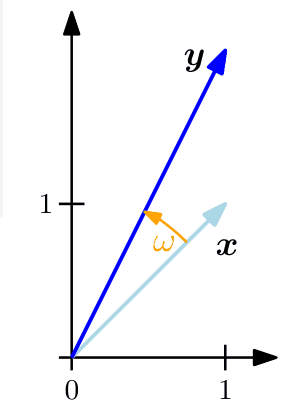
\includegraphics[width=320pt,keepaspectratio]{docs/images/Figure3.5.png}
\caption*{\refstepcounter{figcounter}\label{fig:3-5}图~\thefigcounter 两个向量 x, y 之间的夹角 ω 是通过内积计算的。}
\end{figure}


内积的一个关键特性在于，它还允许我们刻画正交的向量。

\textbf{定义 3.7}（正交性）。两个向量 $ \boldsymbol{x} $ 和 $ \boldsymbol{y} $ 是 \emph{正交的（orthogonal）} 当且仅当 $ \langle \boldsymbol{x}, \boldsymbol{y} \rangle = 0 $，我们记作 $ \boldsymbol{x} \perp \boldsymbol{y} $。如果此外还有 $ \|\boldsymbol{x}\| = 1 = \|\boldsymbol{y}\| $，即这两个向量是单位向量，则称 $ \boldsymbol{x} $ 和 $ \boldsymbol{y} $ 是 \emph{标准正交的（orthonormal）} 。

该定义的一个推论是，零向量与向量空间中的每一个向量都是正交的。

\emph{备注} 。正交性是将垂直概念推广到不一定为点积的双线性形式。在我们的语境中，从几何意义上讲，我们可以将正交向量看作关于特定内积成直角的向量。♦


\begin{figure}[H]
\centering
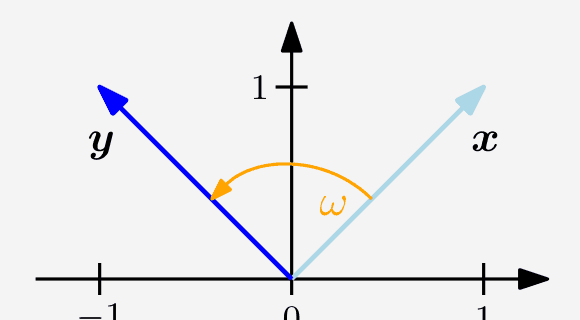
\includegraphics[width=0.92\textwidth,keepaspectratio]{docs/images/Figure3.6.png}
\caption*{\refstepcounter{figcounter}\label{fig:3-6}图~\thefigcounter 两个向量 x, y 之间的夹角 ω 会根据所选内积的不同而发生改变。}
\end{figure}


\begin{notebox}
\textbf{例 3.7（正交向量）}
\end{notebox}

\begin{notebox}
考虑两个向量 $ \boldsymbol{x} = [1, 1]^\top, \boldsymbol{y} = [-1, 1]^\top \in \mathbb{R}^2 $；参见图~\ref{fig:3-6}。我们希望使用两种不同的内积来确定它们之间的夹角 $ \omega $。以点积作为内积，得到 $ \boldsymbol{x} $ 与 $ \boldsymbol{y} $ 之间的夹角 $ \omega $ 为 $ 90^\circ $，从而 $ \boldsymbol{x} \perp \boldsymbol{y} $。然而，如果我们选择内积：

\begin{equation}
\langle \boldsymbol{x}, \boldsymbol{y} \rangle = \boldsymbol{x}^\top \begin{bmatrix} 2 & 0 \\ 0 & 1 \end{bmatrix} \boldsymbol{y}
\tag{3.27}\label{eq:3-27}
\end{equation}

则 $ \boldsymbol{x} $ 与 $ \boldsymbol{y} $ 之间的夹角 $ \omega $ 由下式给出：

\begin{equation}
\cos \omega = \frac{\langle \boldsymbol{x}, \boldsymbol{y} \rangle}{\|\boldsymbol{x}\| \|\boldsymbol{y}\|} = -\frac{1}{3} \implies \omega \approx 1.91\text{ rad} \approx 109.5^\circ
\tag{3.28}\label{eq:3-28}
\end{equation}

此时 $ \boldsymbol{x} $ 与 $ \boldsymbol{y} $ 并不正交。因此，关于某一种内积正交的向量，关于另一种不同的内积并不一定正交。
\end{notebox}

\textbf{定义 3.8}（正交矩阵）。方阵 $ \boldsymbol{A} \in \mathbb{R}^{n \times n} $ 是 \emph{正交矩阵（orthogonal matrix）} 当且仅当其列向量是标准正交的，从而满足：

\begin{equation}
\boldsymbol{A} \boldsymbol{A}^\top = \boldsymbol{I} = \boldsymbol{A}^\top \boldsymbol{A}
\tag{3.29}\label{eq:3-29}
\end{equation}

这蕴含着：

\begin{equation}
\boldsymbol{A}^{-1} = \boldsymbol{A}^\top
\tag{3.30}\label{eq:3-30}
\end{equation}

即逆矩阵只需通过对该矩阵进行转置即可得到。

\begin{notebox}
习惯上称这类矩阵为“正交矩阵”，但更精确的表述应该是“标准正交矩阵”。
\end{notebox}

由正交矩阵定义的变换十分特殊，因为向量 $ \boldsymbol{x} $ 在利用正交矩阵 $ \boldsymbol{A} $ 进行变换时其长度保持不变。对于点积，我们有：

\begin{equation}
\begin{adjustbox}{max width=\linewidth}
\|\boldsymbol{A} \boldsymbol{x}\|^2 = (\boldsymbol{A} \boldsymbol{x})^\top (\boldsymbol{A} \boldsymbol{x}) = \boldsymbol{x}^\top \boldsymbol{A}^\top \boldsymbol{A} \boldsymbol{x} = \boldsymbol{x}^\top \boldsymbol{I} \boldsymbol{x} = \boldsymbol{x}^\top \boldsymbol{x} = \|\boldsymbol{x}\|^2
\end{adjustbox}
\tag{3.31}\label{eq:3-31}
\end{equation}

\begin{notebox}
正交矩阵所对应的变换保持距离和夹角不变。
\end{notebox}

此外，利用内积度量的任意两个向量 $ \boldsymbol{x}, \boldsymbol{y} $ 之间的夹角，在同时使用正交矩阵 $ \boldsymbol{A} $ 对它们进行变换时也保持不变。假设以内积为点积，则像 $ \boldsymbol{A} \boldsymbol{x} $ 与 $ \boldsymbol{A} \boldsymbol{y} $ 之间的夹角由下式给出：

\begin{equation}
\begin{adjustbox}{max width=\linewidth}
\cos \omega = \frac{(\boldsymbol{A} \boldsymbol{x})^\top (\boldsymbol{A} \boldsymbol{y})}{\|\boldsymbol{A} \boldsymbol{x}\| \|\boldsymbol{A} \boldsymbol{y}\|} = \frac{\boldsymbol{x}^\top \boldsymbol{A}^\top \boldsymbol{A} \boldsymbol{y}}{\sqrt{\boldsymbol{x}^\top \boldsymbol{A}^\top \boldsymbol{A} \boldsymbol{x} \, \boldsymbol{y}^\top \boldsymbol{A}^\top \boldsymbol{A} \boldsymbol{y}}} = \frac{\boldsymbol{x}^\top \boldsymbol{y}}{\|\boldsymbol{x}\| \|\boldsymbol{y}\|}
\end{adjustbox}
\tag{3.32}\label{eq:3-32}
\end{equation}

这正好给出了 $ \boldsymbol{x} $ 与 $ \boldsymbol{y} $ 之间的夹角。这意味着满足 $ \boldsymbol{A}^\top = \boldsymbol{A}^{-1} $ 的正交矩阵 $ \boldsymbol{A} $ 既保持夹角不变，也保持距离不变。事实上，正交矩阵所定义的变换是旋转（可能伴随翻转）。在第 3.9 节中，我们将讨论有关旋转的更多细节。

\section*{3.5 标准正交基}
\addcontentsline{toc}{section}{3.5 标准正交基}
\label{sec:3.5}

在第 2.6.1 节中，我们刻画了基向量的性质，并发现一个 $ n $ 维向量空间中需要 $ n $ 个基向量，即 $ n $ 个线性无关的向量。在第 3.3 节和第 3.4 节中，我们利用内积计算了向量的长度以及向量之间的夹角。接下来，我们将讨论基向量两两正交且每个基向量长度均为 1 的特殊情形。我们将这样的基称为标准正交基。

下面我们更形式化地引入该概念。

\textbf{定义 3.9}（标准正交基）。考虑一个 $ n $ 维向量空间 $ V $ 以及 $ V $ 的一组基 $ \{\boldsymbol{b}_1, \ldots, \boldsymbol{b}_n\} $。如果对于所有 $ i, j = 1, \ldots, n $，满足：

\begin{equation}
\langle \boldsymbol{b}_i, \boldsymbol{b}_j \rangle = 0 \quad (i \neq j)
\tag{3.33}\label{eq:3-33}
\end{equation}

\begin{equation}
\langle \boldsymbol{b}_i, \boldsymbol{b}_i \rangle = 1
\tag{3.34}\label{eq:3-34}
\end{equation}

则称该基为 \emph{标准正交基（orthonormal basis, ONB）} 。如果仅满足式~\eqref{eq:3-33}，则称该基为 \emph{正交基（orthogonal basis）} 。注意，式~\eqref{eq:3-34} 蕴含着每个基向量的长度/范数均为 1。

回想第 2.6.1 节，我们可以使用高斯消元法来寻找一组向量所张成的向量空间的一组基。假设给定一组非正交且未归一化的基向量 $ \{\tilde{\boldsymbol{b}}_1, \ldots, \tilde{\boldsymbol{b}}_n\} $。我们将它们拼接成矩阵 $ \tilde{\boldsymbol{B}} = [\tilde{\boldsymbol{b}}_1, \ldots, \tilde{\boldsymbol{b}}_n] $，并对增广矩阵（第 2.3.2 节）$ [\tilde{\boldsymbol{B}}\tilde{\boldsymbol{B}}^\top \mid \tilde{\boldsymbol{B}}] $ 应用高斯消元法以获得一组标准正交基。这种迭代构建标准正交基 $ \{\boldsymbol{b}_1, \ldots, \boldsymbol{b}_n\} $ 的构造性方法称为 \emph{格拉姆-施密特过程（Gram-Schmidt process）} （Strang, 2003）。

\begin{notebox}
\textbf{例 3.8（标准正交基）}
\end{notebox}

\begin{notebox}
欧几里得向量空间 $ \mathbb{R}^n $ 的标准基（canonical/standard basis）是一组标准正交基，其中内积为向量的点积。 在 $ \mathbb{R}^2 $ 中，向量：

\begin{equation}
\boldsymbol{b}_1 = \frac{1}{\sqrt{2}} \begin{bmatrix} 1 \\ 1 \end{bmatrix}, \quad \boldsymbol{b}_2 = \frac{1}{\sqrt{2}} \begin{bmatrix} 1 \\ -1 \end{bmatrix}
\tag{3.35}\label{eq:3-35}
\end{equation}

构成一组标准正交基，因为 $ \boldsymbol{b}_1^\top \boldsymbol{b}_2 = 0 $ 且 $ \|\boldsymbol{b}_1\| = 1 = \|\boldsymbol{b}_2\| $。
\end{notebox}

我们将在第 12 章和第 10 章讨论支持向量机与主成分分析时应用标准正交基的概念。

\section*{3.6 正交补}
\addcontentsline{toc}{section}{3.6 正交补}
\label{sec:3.6}

在定义了正交性之后，我们现在考察相互正交的向量空间。这将在第 10 章从几何视角讨论线性降维时发挥重要作用。

考虑一个 $ D $ 维向量空间 $ V $ 及其一个 $ M $ 维子空间 $ U \subseteq V $。那么它的 \emph{正交补（orthogonal complement）} $ U^\perp $ 是 $ V $ 的一个 $ (D - M) $ 维子空间，并且包含 $ V $ 中与 $ U $ 中每一个向量都正交的所有向量。此外，$ U \cap U^\perp = \{\boldsymbol{0}\} $，使得任意向量 $ \boldsymbol{x} \in V $ 都可以唯一分解为：

\begin{equation}
\boldsymbol{x} = \sum_{m=1}^M \lambda_m \boldsymbol{b}_m + \sum_{j=1}^{D-M} \psi_j \boldsymbol{b}_j^\perp, \quad \lambda_m, \psi_j \in \mathbb{R}
\tag{3.36}\label{eq:3-36}
\end{equation}

其中 $ (\boldsymbol{b}_1, \ldots, \boldsymbol{b}_M) $ 是 $ U $ 的一组基，而 $ (\boldsymbol{b}_1^\perp, \ldots, \boldsymbol{b}_{D-M}^\perp) $ 是 $ U^\perp $ 的一组基。

因此，正交补也可以用来描述三维向量空间中的平面 $ U $（二维子空间）。更具体地，满足 $ \|\boldsymbol{w}\| = 1 $ 且与平面 $ U $ 正交的向量 $ \boldsymbol{w} $ 是 $ U^\perp $ 的基向量。图~\ref{fig:3-7} 说明了这种设定。所有与 $ \boldsymbol{w} $ 正交的向量（根据构造）必然落在平面 $ U $ 内。向量 $ \boldsymbol{w} $ 称为 $ U $ 的 \emph{法向量（normal vector）} 。


\begin{figure}[H]
\centering
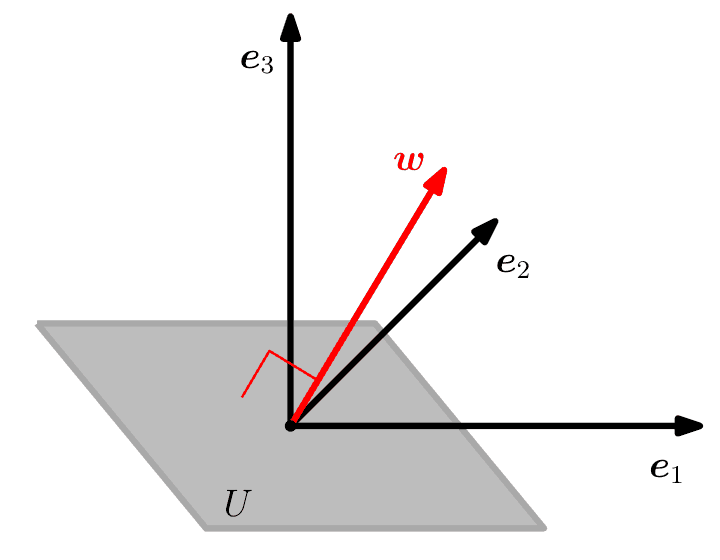
\includegraphics[width=0.92\textwidth,keepaspectratio]{docs/images/Figure3.7.png}
\caption*{\refstepcounter{figcounter}\label{fig:3-7}图~\thefigcounter 三维向量空间中的平面 U 可以通过其法向量来描述，该法向量张成了其正交补空间 U⊥。}
\end{figure}


通常，正交补可以用来描述 $ n $ 维向量空间与仿射空间中的超平面。

\section*{3.7 函数的内积}
\addcontentsline{toc}{section}{3.7 函数的内积}
\label{sec:3.7}

到目前为止，我们考察了内积在计算长度、夹角和距离方面的性质。我们一直聚焦于有限维向量的内积。接下来，我们将看一个不同类型向量的内积示例：函数的内积。

迄今为止我们讨论的内积都是针对具有有限个分量的向量定义的。我们可以将向量 $ \boldsymbol{x} \in \mathbb{R}^n $ 视为具有 $ n $ 个函数值的函数。内积的概念可以推广到具有无限个分量的向量（可数无穷）以及连续值函数（不可数无穷）。此时，向量各分量的求和（例如参见式~\eqref{eq:3-5}）将转变为积分。

两个函数 $ u : \mathbb{R} \to \mathbb{R} $ 和 $ v : \mathbb{R} \to \mathbb{R} $ 的内积可以定义为定积分：

\begin{equation}
\langle u, v \rangle := \int_a^b u(x) v(x) \, \mathrm{d}x
\tag{3.37}\label{eq:3-37}
\end{equation}

其中积分下限和上限分别满足 $ a, b < \infty $。与通常的内积一样，我们也可以通过考察内积来定义范数和正交性。如果式~\eqref{eq:3-37} 的计算结果为 0，则函数 $ u $ 和 $ v $ 是正交的。为了使上述内积在数学上更加严格，我们需要考虑测度以及积分的定义，这引出了 \emph{希尔伯特空间（Hilbert space）} 的定义。此外，与有限维向量上的内积不同，函数上的内积可能会发散（具有无穷大的值）。所有这些都需要深入探讨实分析和泛函分析中更错综复杂的细节，本书对此不做展开。

\begin{notebox}
\textbf{例 3.9（函数的内积）}
\end{notebox}

\begin{notebox}
如果我们选择 $ u = \sin(x) $ 和 $ v = \cos(x) $，式~\eqref{eq:3-37} 中的被积函数 $ f(x) = u(x)v(x) $ 如图~\ref{fig:3-8} 所示。我们看到该函数是奇函数，即 $ f(-x) = -f(x) $。因此，在积分限为 $ a = -\pi, b = \pi $ 时，该乘积的积分计算结果为 0。所以，$ \sin $ 和 $ \cos $ 是正交函数。
\end{notebox}


\begin{figure}[H]
\centering
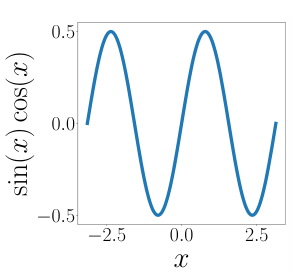
\includegraphics[width=0.92\textwidth,keepaspectratio]{docs/images/Figure3.8.png}
\caption*{\refstepcounter{figcounter}\label{fig:3-8}图~\thefigcounter 奇函数 f(x) = sin(x)cos(x)。}
\end{figure}


\emph{备注} 。同样地，如果从 $ -\pi $ 到 $ \pi $ 积分，函数集合：

\begin{equation}
\{1, \cos(x), \cos(2x), \cos(3x), \ldots\}
\tag{3.38}\label{eq:3-38}
\end{equation}

也是正交的，即其中任意两个不同的函数之间都相互正交。式~\eqref{eq:3-38} 中的函数集合张成了在 $ [-\pi, \pi) $ 上为偶函数且具周期性的函数的一个很大子空间，将函数投影到该子空间上正是 \emph{傅里叶级数（Fourier series）} 背后的基本思想。♦

在第 6.4.6 节中，我们将考察第二类非常规内积：随机变量的内积。

\section*{3.8 正交投影}
\addcontentsline{toc}{section}{3.8 正交投影}
\label{sec:3.8}

投影是一类重要的线性变换（除旋转和翻转之外），在图形学、编码理论、统计学和机器学习中发挥着重要作用。在机器学习中，我们经常处理高维数据。高维数据通常难以分析或可视化。然而，高维数据往往具有这样的性质：只有少数几个维度包含了大部分信息，而大多数其他维度对于描述数据的关键属性并不是必需的。当我们压缩或可视化高维数据时，会丢失信息。为了尽量减少这种压缩损失，我们理想的做法是找到数据中信息量最丰富的维度。正如第 1 章中所讨论的，数据可以表示为向量（“特征（feature）”是数据表示的常用表达），在本章中，我们将讨论一些用于数据压缩的基本工具。更具体地，我们可以将原始高维数据投影到较低维的特征空间中，并在这个较低维空间中开展工作，以了解更多关于数据集的信息并提取相关的模式。例如，机器学习算法，如 Pearson（1901）和 Hotelling（1933）提出的主成分分析（PCA）以及深度神经网络（例如深度自动编码器（Deng et al., 2010）），都大量利用了降维的思想。在下文中，我们将重点讨论正交投影，我们将在第 10 章中将其用于线性降维，在第 12 章中用于分类。甚至我们在第 9 章讨论的线性回归，也可以使用正交投影来解释。对于给定的低维子空间，高维数据的正交投影能够保留尽可能多的信息，并使原始数据与相应投影之间的差异/误差最小化。图~\ref{fig:3-9} 给出了这种正交投影的示意图。在我们详细介绍如何获得这些投影之前，先来定义什么是投影。


\begin{figure}[H]
\centering
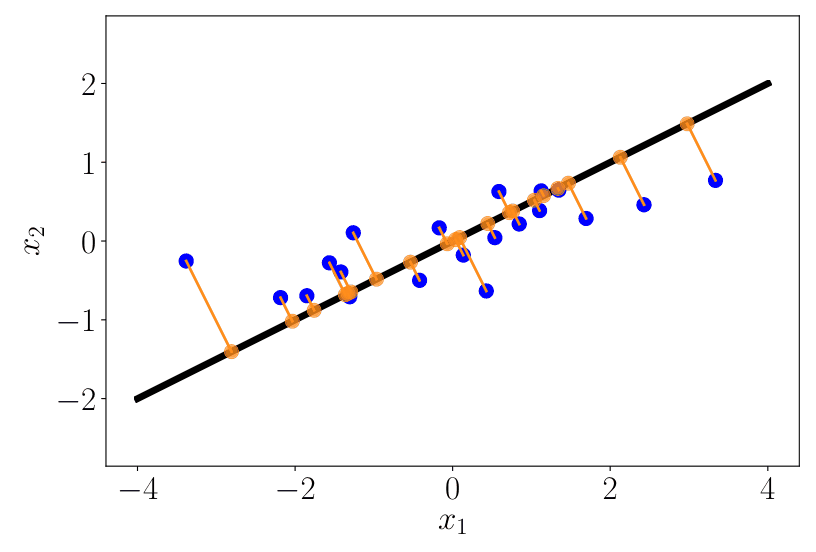
\includegraphics[width=0.92\textwidth,keepaspectratio]{docs/images/Figure3.9.png}
\caption*{\refstepcounter{figcounter}\label{fig:3-9}图~\thefigcounter 二维数据集（蓝色圆点）到一维子空间（直线）的正交投影（橙色圆点）。}
\end{figure}


\textbf{定义 3.10}（投影）。设 $ V $ 为向量空间，$ U \subseteq V $ 为 $ V $ 的子空间。如果一个线性映射 $ \pi : V \to U $ 满足：

\begin{equation*}
\pi^2 = \pi \circ \pi = \pi
\end{equation*}

则称其为 \emph{投影（projection）} 。

由于线性映射可以用变换矩阵来表示（参见第 2.7 节），上述定义同样适用于一类特殊的变换矩阵—— \emph{投影矩阵（projection matrix）} $ \boldsymbol{P}_\pi $，它们具有性质 $ \boldsymbol{P}_\pi^2 = \boldsymbol{P}_\pi $。

在下文中，我们将推导内积空间 $ (\mathbb{R}^n, \langle \cdot, \cdot \rangle) $ 中的向量到子空间的正交投影。我们将从一维子空间开始，一维子空间也称为 \emph{直线（line）} 。若无特别说明，我们默认以内积为点积 $ \langle \boldsymbol{x}, \boldsymbol{y} \rangle = \boldsymbol{x}^\top \boldsymbol{y} $。

\section*{3.8.1 投影到一维子空间（直线）}
\addcontentsline{toc}{subsection}{3.8.1 投影到一维子空间（直线）}

假设给定一条过原点且基向量为 $ \boldsymbol{b} \in \mathbb{R}^n $ 的直线（一维子空间）。该直线是由 $ \boldsymbol{b} $ 张成的一维子空间 $ U \subseteq \mathbb{R}^n $。当我们将 $ \boldsymbol{x} \in \mathbb{R}^n $ 投影到 $ U $ 上时，我们要寻找 $ U $ 中距离 $ \boldsymbol{x} $ 最近的向量 $ \pi_U(\boldsymbol{x}) \in U $。利用几何论证，让我们来刻画投影 $ \pi_U(\boldsymbol{x}) $ 的一些性质（图~\ref{fig:3-10}(a) 给出了示意说明）：

\begin{itemize}
\item 投影 $ \pi_U(\boldsymbol{x}) $ 距离 $ \boldsymbol{x} $ 最近，其中“最近”意味着距离 $ \|\boldsymbol{x} - \pi_U(\boldsymbol{x})\| $ 最小。由此可知，从 $ \pi_U(\boldsymbol{x}) $ 到 $ \boldsymbol{x} $ 的线段 $ \pi_U(\boldsymbol{x}) - \boldsymbol{x} $ 与 $ U $ 正交，因此也与 $ U $ 的基向量 $ \boldsymbol{b} $ 正交。由于向量之间的夹角是通过内积定义的，正交条件给出 $ \langle \pi_U(\boldsymbol{x}) - \boldsymbol{x}, \boldsymbol{b} \rangle = 0 $。
\item $ \boldsymbol{x} $ 在 $ U $ 上的投影 $ \pi_U(\boldsymbol{x}) $ 必然是 $ U $ 中的元素，因此它是张成 $ U $ 的基向量 $ \boldsymbol{b} $ 的倍数。因此，对于某个 $ \lambda \in \mathbb{R} $，有 $ \pi_U(\boldsymbol{x}) = \lambda \boldsymbol{b} $（此时 $ \lambda $ 是 $ \pi_U(\boldsymbol{x}) $ 关于基向量 $ \boldsymbol{b} $ 的坐标）。
\end{itemize}


\begin{figure}[H]
\centering
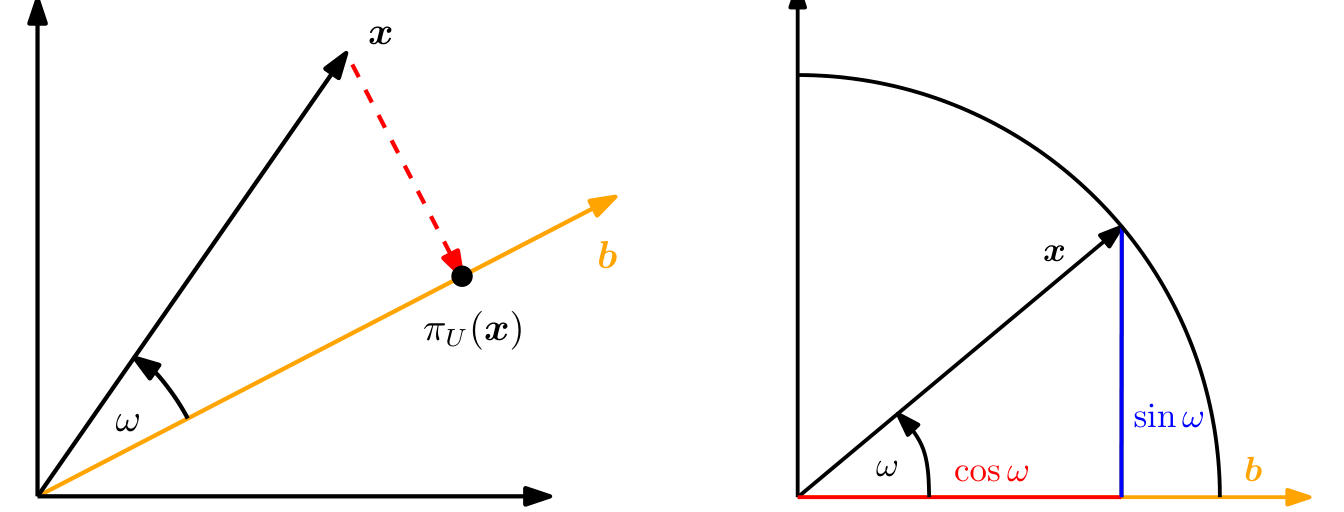
\includegraphics[width=0.92\textwidth,keepaspectratio]{docs/images/Figure3.10.png}
\caption*{\refstepcounter{figcounter}\label{fig:3-10}图~\thefigcounter 投影到一维子空间的示例。(a) 将 x ∈ ℝ² 投影到具有基向量 b 的子空间 U 上；(b) 将 ∥x∥ = 1 的二维向量 x 投影到由 b 张成的一维子空间上。}
\end{figure}


在接下来的三个步骤中，我们确定坐标 $ \lambda $、投影点 $ \pi_U(\boldsymbol{x}) \in U $ 以及将任意 $ \boldsymbol{x} \in \mathbb{R}^n $ 映射到 $ U $ 上的投影矩阵 $ \boldsymbol{P}_\pi $：

\begin{enumerate}
\item \textbf{求坐标 $ \lambda $}。正交条件给出：
\end{enumerate}

\begin{equation}
\langle \boldsymbol{x} - \pi_U(\boldsymbol{x}), \boldsymbol{b} \rangle = 0 \stackrel{\pi_U(\boldsymbol{x}) = \lambda \boldsymbol{b}}{\iff} \langle \boldsymbol{x} - \lambda \boldsymbol{b}, \boldsymbol{b} \rangle = 0
\tag{3.39}\label{eq:3-39}
\end{equation}

现在我们可以利用内积的双线性性质，得到：

\begin{equation}
\begin{adjustbox}{max width=\linewidth}
\langle \boldsymbol{x}, \boldsymbol{b} \rangle - \lambda \langle \boldsymbol{b}, \boldsymbol{b} \rangle = 0 \iff \lambda = \frac{\langle \boldsymbol{x}, \boldsymbol{b} \rangle}{\langle \boldsymbol{b}, \boldsymbol{b} \rangle} = \frac{\langle \boldsymbol{b}, \boldsymbol{x} \rangle}{\|\boldsymbol{b}\|^2}
\end{adjustbox}
\tag{3.40}\label{eq:3-40}
\end{equation}

在最后一步中，我们利用了内积是对称的事实。对于一般的内积，若 $ \|\boldsymbol{b}\| = 1 $，则有 $ \lambda = \langle \boldsymbol{x}, \boldsymbol{b} \rangle $。如果我们将 $ \langle \cdot, \cdot \rangle $ 选取为点积，则得到：

\begin{equation}
\lambda = \frac{\boldsymbol{b}^\top \boldsymbol{x}}{\boldsymbol{b}^\top \boldsymbol{b}} = \frac{\boldsymbol{b}^\top \boldsymbol{x}}{\|\boldsymbol{b}\|^2}
\tag{3.41}\label{eq:3-41}
\end{equation}

若 $ \|\boldsymbol{b}\| = 1 $，则投影的坐标 $ \lambda $ 由 $ \boldsymbol{b}^\top \boldsymbol{x} $ 给出。

\begin{enumerate}
\item \textbf{求投影点 $ \pi_U(\boldsymbol{x}) \in U $}。由于 $ \pi_U(\boldsymbol{x}) = \lambda \boldsymbol{b} $，结合式~\eqref{eq:3-40} 我们立即得到：
\end{enumerate}

\begin{equation}
\begin{adjustbox}{max width=\linewidth}
\pi_U(\boldsymbol{x}) = \lambda \boldsymbol{b} = \frac{\langle \boldsymbol{x}, \boldsymbol{b} \rangle}{\|\boldsymbol{b}\|^2} \boldsymbol{b} = \frac{\boldsymbol{b}^\top \boldsymbol{x}}{\|\boldsymbol{b}\|^2} \boldsymbol{b}
\end{adjustbox}
\tag{3.42}\label{eq:3-42}
\end{equation}

其中最后一个等号仅对点积成立。我们还可以根据定义 3.1 计算 $ \pi_U(\boldsymbol{x}) $ 的长度为：

\begin{equation}
\|\pi_U(\boldsymbol{x})\| = \|\lambda \boldsymbol{b}\| = |\lambda| \|\boldsymbol{b}\|
\tag{3.43}\label{eq:3-43}
\end{equation}

因此，投影的长度是 $ |\lambda| $ 乘以 $ \boldsymbol{b} $ 的长度。这进一步加深了直观理解：$ \lambda $ 是 $ \pi_U(\boldsymbol{x}) $ 关于张成一维子空间 $ U $ 的基向量 $ \boldsymbol{b} $ 的坐标。 如果我们使用点积作为内积，可得：

\begin{equation}
\begin{adjustbox}{max width=\linewidth}
\|\pi_U(\boldsymbol{x})\| \stackrel{(3.42)}{=} \frac{|\boldsymbol{b}^\top \boldsymbol{x}|}{\|\boldsymbol{b}\|^2} \|\boldsymbol{b}\| \stackrel{(3.25)}{=} \frac{|\cos \omega| \|\boldsymbol{x}\| \|\boldsymbol{b}\| \|\boldsymbol{b}\|}{\|\boldsymbol{b}\|^2} = |\cos \omega| \|\boldsymbol{x}\|
\end{adjustbox}
\tag{3.44}\label{eq:3-44}
\end{equation}

这里 $ \omega $ 是 $ \boldsymbol{x} $ 与 $ \boldsymbol{b} $ 之间的夹角。这个方程应该在三角学中很熟悉：如果 $ \|\boldsymbol{x}\| = 1 $，则 $ \boldsymbol{x} $ 落在单位圆上。由此可知，投影到由 $ \boldsymbol{b} $ 张成的水平轴（水平轴是一个一维子空间）上恰好是 $ \cos \omega $，对应向量的长度为 $ \|\pi_U(\boldsymbol{x})\| = |\cos \omega| $。图~\ref{fig:3-10}(b) 给出了示意说明。

\begin{enumerate}
\item \textbf{求投影矩阵 $ \boldsymbol{P}_\pi $}。我们知道投影是一个线性映射（参见定义 3.10）。因此，存在一个投影矩阵 $ \boldsymbol{P}_\pi $，使得 $ \pi_U(\boldsymbol{x}) = \boldsymbol{P}_\pi \boldsymbol{x} $。以点积为内积，并且根据：
\end{enumerate}

\begin{equation}
\begin{adjustbox}{max width=\linewidth}
\pi_U(\boldsymbol{x}) = \lambda \boldsymbol{b} = \boldsymbol{b} \lambda = \boldsymbol{b} \frac{\boldsymbol{b}^\top \boldsymbol{x}}{\|\boldsymbol{b}\|^2} = \frac{\boldsymbol{b} \boldsymbol{b}^\top}{\|\boldsymbol{b}\|^2} \boldsymbol{x}
\end{adjustbox}
\tag{3.45}\label{eq:3-45}
\end{equation}

我们立即看出：

\begin{equation}
\boldsymbol{P}_\pi = \frac{\boldsymbol{b} \boldsymbol{b}^\top}{\|\boldsymbol{b}\|^2}
\tag{3.46}\label{eq:3-46}
\end{equation}

注意 $ \boldsymbol{b} \boldsymbol{b}^\top $（以及随之而来的 $ \boldsymbol{P}_\pi $）是一个（秩为 1 的）对称矩阵（投影矩阵总是对称的），而 $ \|\boldsymbol{b}\|^2 = \langle \boldsymbol{b}, \boldsymbol{b} \rangle $ 是一个标量。 投影矩阵 $ \boldsymbol{P}_\pi $ 将任意向量 $ \boldsymbol{x} \in \mathbb{R}^n $ 投影到过原点且方向为 $ \boldsymbol{b} $ 的直线上（等价地，投影到由 $ \boldsymbol{b} $ 张成的子空间 $ U $ 上）。

\emph{备注} 。投影 $ \pi_U(\boldsymbol{x}) \in \mathbb{R}^n $ 仍然是一个 $ n $ 维向量，而不是标量。然而，如果我们想关于张成子空间 $ U $ 的基向量 $ \boldsymbol{b} $ 来表示该投影，则不再需要 $ n $ 个坐标，而只需要一个单独的坐标：$ \lambda $。♦

\begin{notebox}
\textbf{例 3.10（投影到直线上）}
\end{notebox}

\begin{notebox}
求过原点且由 $ \boldsymbol{b} = [1, 2, 2]^\top $ 张成的直线上的投影矩阵 $ \boldsymbol{P}_\pi $。$ \boldsymbol{b} $ 是一维子空间（过原点的直线）的方向和基。 利用式~\eqref{eq:3-46}，我们得到：

\begin{equation}
\begin{adjustbox}{max width=\linewidth}
\boldsymbol{P}_\pi = \frac{\boldsymbol{b} \boldsymbol{b}^\top}{\boldsymbol{b}^\top \boldsymbol{b}} = \frac{1}{9} \begin{bmatrix} 1 \\ 2 \\ 2 \end{bmatrix} \begin{bmatrix} 1 & 2 & 2 \end{bmatrix} = \frac{1}{9} \begin{bmatrix} 1 & 2 & 2 \\ 2 & 4 & 4 \\ 2 & 4 & 4 \end{bmatrix}
\end{adjustbox}
\tag{3.47}\label{eq:3-47}
\end{equation}

现在让我们选择一个具体的 $ \boldsymbol{x} $，看看它是否落在由 $ \boldsymbol{b} $ 张成的子空间中。对于 $ \boldsymbol{x} = [1, 1, 1]^\top $，投影为：

\begin{equation}
\begin{adjustbox}{max width=\linewidth}
\pi_U(\boldsymbol{x}) = \boldsymbol{P}_\pi \boldsymbol{x} = \frac{1}{9} \begin{bmatrix} 1 & 2 & 2 \\ 2 & 4 & 4 \\ 2 & 4 & 4 \end{bmatrix} \begin{bmatrix} 1 \\ 1 \\ 1 \end{bmatrix} = \frac{1}{9} \begin{bmatrix} 5 \\ 10 \\ 10 \end{bmatrix} \in \text{span}\left[\begin{bmatrix} 1 \\ 2 \\ 2 \end{bmatrix}\right]
\end{adjustbox}
\tag{3.48}\label{eq:3-48}
\end{equation}

注意，将 $ \boldsymbol{P}_\pi $ 应用于 $ \pi_U(\boldsymbol{x}) $ 不会改变任何东西，即 $ \boldsymbol{P}_\pi \pi_U(\boldsymbol{x}) = \pi_U(\boldsymbol{x}) $。这是符合预期的，因为根据定义 3.10，我们知道投影矩阵 $ \boldsymbol{P}_\pi $ 对所有 $ \boldsymbol{x} $ 都满足 $ \boldsymbol{P}_\pi^2 \boldsymbol{x} = \boldsymbol{P}_\pi \boldsymbol{x} $。
\end{notebox}

\emph{备注} 。利用第 4 章的结果，我们可以证明 $ \pi_U(\boldsymbol{x}) $ 是 $ \boldsymbol{P}_\pi $ 的特征向量，对应的特征值为 1。♦

\section*{3.8.2 投影到一般子空间}
\addcontentsline{toc}{subsection}{3.8.2 投影到一般子空间}

下面我们考察向量 $ \boldsymbol{x} \in \mathbb{R}^n $ 到更低维子空间 $ U \subseteq \mathbb{R}^n $ 上的正交投影，其中 $ \dim(U) = m \geqslant 1 $。图~\ref{fig:3-11} 给出了直观示意。

（若 $ U $ 由一组不是基的生成向量给出，请在继续之前务必先确定一组基 $ \boldsymbol{b}_1, \ldots, \boldsymbol{b}_m $。）


\begin{figure}[H]
\centering
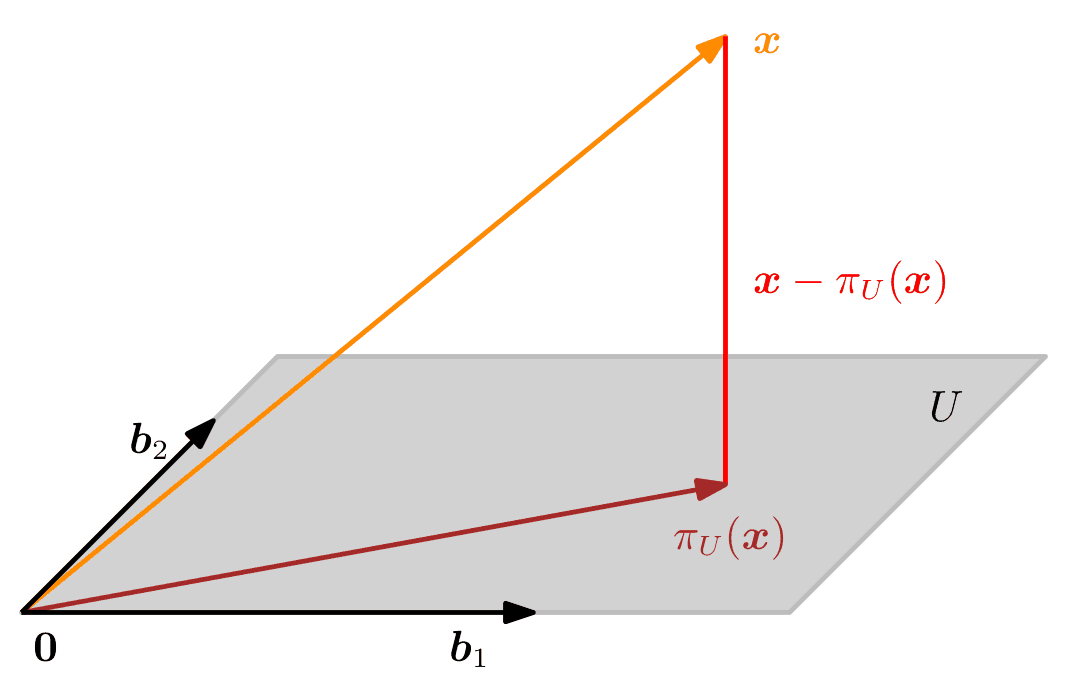
\includegraphics[width=0.92\textwidth,keepaspectratio]{docs/images/Figure3.11.png}
\caption*{\refstepcounter{figcounter}\label{fig:3-11}图~\thefigcounter 投影到具有基 b₁, b₂ 的二维子空间 U 上。x ∈ ℝ³ 在 U 上的投影 πU(x) 可以表示为 b₁, b₂ 的线性组合，位移向量 x − πU(x) 同时与 b₁ 和 b₂ 正交。}
\end{figure}


假设 $ (\boldsymbol{b}_1, \ldots, \boldsymbol{b}_m) $ 是 $ U $ 的一组有序基。$ U $ 上的任何投影 $ \pi_U(\boldsymbol{x}) $ 必然是 $ U $ 中的元素。因此，它们可以表示为 $ U $ 的基向量 $ \boldsymbol{b}_1, \ldots, \boldsymbol{b}_m $ 的线性组合，即 $ \pi_U(\boldsymbol{x}) = \sum_{i=1}^m \lambda_i \boldsymbol{b}_i $。基向量构成矩阵 $ \boldsymbol{B} \in \mathbb{R}^{n \times m} $ 的列，其中 $ \boldsymbol{B} = [\boldsymbol{b}_1, \ldots, \boldsymbol{b}_m] $。

与一维情况类似，我们遵循三步过程来寻找投影 $ \pi_U(\boldsymbol{x}) $ 和投影矩阵 $ \boldsymbol{P}_\pi $：

\begin{enumerate}
\item \textbf{求投影的坐标 $ \lambda_1, \ldots, \lambda_m $}（关于 $ U $ 的基），使得线性组合：
\end{enumerate}

\begin{equation}
\pi_U(\boldsymbol{x}) = \sum_{i=1}^m \lambda_i \boldsymbol{b}_i = \boldsymbol{B} \boldsymbol{\lambda}
\tag{3.49}\label{eq:3-49}
\end{equation}

\begin{equation}
\boldsymbol{B} = [\boldsymbol{b}_1, \ldots, \boldsymbol{b}_m] \in \mathbb{R}^{n \times m}, \quad \boldsymbol{\lambda} = [\lambda_1, \ldots, \lambda_m]^\top \in \mathbb{R}^m
\tag{3.50}\label{eq:3-50}
\end{equation}

距离 $ \boldsymbol{x} \in \mathbb{R}^n $ 最近。与一维情况相同，“最近”意味着“距离最小”，这意味着连接 $ \pi_U(\boldsymbol{x}) \in U $ 与 $ \boldsymbol{x} \in \mathbb{R}^n $ 的向量必须与 $ U $ 的所有基向量都正交。因此，我们得到 $ m $ 个联立条件（假设以内积为点积）：

\begin{equation}
\langle \boldsymbol{b}_1, \boldsymbol{x} - \pi_U(\boldsymbol{x}) \rangle = \boldsymbol{b}_1^\top (\boldsymbol{x} - \pi_U(\boldsymbol{x})) = 0
\tag{3.51}\label{eq:3-51}
\end{equation}

\begin{equation*}
\vdots
\end{equation*}

\begin{equation}
\langle \boldsymbol{b}_m, \boldsymbol{x} - \pi_U(\boldsymbol{x}) \rangle = \boldsymbol{b}_m^\top (\boldsymbol{x} - \pi_U(\boldsymbol{x})) = 0
\tag{3.52}\label{eq:3-52}
\end{equation}

结合 $ \pi_U(\boldsymbol{x}) = \boldsymbol{B} \boldsymbol{\lambda} $，可以写为：

\begin{equation}
\boldsymbol{b}_1^\top (\boldsymbol{x} - \boldsymbol{B} \boldsymbol{\lambda}) = 0
\tag{3.53}\label{eq:3-53}
\end{equation}

\begin{equation*}
\vdots
\end{equation*}

\begin{equation}
\boldsymbol{b}_m^\top (\boldsymbol{x} - \boldsymbol{B} \boldsymbol{\lambda}) = 0
\tag{3.54}\label{eq:3-54}
\end{equation}

从而我们得到一个齐次线性方程组：

\begin{equation}
\begin{adjustbox}{max width=\linewidth}
\begin{bmatrix} \boldsymbol{b}_1^\top \\ \vdots \\ \boldsymbol{b}_m^\top \end{bmatrix} (\boldsymbol{x} - \boldsymbol{B} \boldsymbol{\lambda}) = \boldsymbol{0} \iff \boldsymbol{B}^\top (\boldsymbol{x} - \boldsymbol{B} \boldsymbol{\lambda}) = \boldsymbol{0}
\end{adjustbox}
\tag{3.55}\label{eq:3-55}
\end{equation}

\begin{equation}
\iff \boldsymbol{B}^\top \boldsymbol{B} \boldsymbol{\lambda} = \boldsymbol{B}^\top \boldsymbol{x}
\tag{3.56}\label{eq:3-56}
\end{equation}

最后一个表达式称为 \emph{正规方程（normal equation）} 。由于 $ \boldsymbol{b}_1, \ldots, \boldsymbol{b}_m $ 是 $ U $ 的一组基，因此线性无关，$ \boldsymbol{B}^\top \boldsymbol{B} \in \mathbb{R}^{m \times m} $ 是非奇异（正则）的且可逆。这使得我们能够解出系数/坐标：

\begin{equation}
\boldsymbol{\lambda} = (\boldsymbol{B}^\top \boldsymbol{B})^{-1} \boldsymbol{B}^\top \boldsymbol{x}
\tag{3.57}\label{eq:3-57}
\end{equation}

矩阵 $ (\boldsymbol{B}^\top \boldsymbol{B})^{-1} \boldsymbol{B}^\top $ 也称为 $ \boldsymbol{B} $ 的 \emph{伪逆（pseudo-inverse）} ，它可以针对非方阵 $ \boldsymbol{B} $ 进行计算。它仅要求 $ \boldsymbol{B}^\top \boldsymbol{B} $ 是正定的，当 $ \boldsymbol{B} $ 列满秩时便满足此条件。在实际应用中（例如线性回归），我们经常在 $ \boldsymbol{B}^\top \boldsymbol{B} $ 上添加一个“微扰项/抖动项（jitter term）” $ \epsilon \boldsymbol{I} $，以保证提高数值稳定性和正定性。这种“岭（ridge）”可以通过贝叶斯推断严格导出，详见第 9 章。

\begin{enumerate}
\item \textbf{求投影点 $ \pi_U(\boldsymbol{x}) \in U $}。我们已经确定 $ \pi_U(\boldsymbol{x}) = \boldsymbol{B} \boldsymbol{\lambda} $。因此，结合式~\eqref{eq:3-57}：
\end{enumerate}

\begin{equation}
\pi_U(\boldsymbol{x}) = \boldsymbol{B} (\boldsymbol{B}^\top \boldsymbol{B})^{-1} \boldsymbol{B}^\top \boldsymbol{x}
\tag{3.58}\label{eq:3-58}
\end{equation}

\begin{enumerate}
\item \textbf{求投影矩阵 $ \boldsymbol{P}_\pi $}。从式~\eqref{eq:3-58} 中，我们可以立即看出求解 $ \boldsymbol{P}_\pi \boldsymbol{x} = \pi_U(\boldsymbol{x}) $ 的投影矩阵必然是：
\end{enumerate}

\begin{equation}
\boldsymbol{P}_\pi = \boldsymbol{B} (\boldsymbol{B}^\top \boldsymbol{B})^{-1} \boldsymbol{B}^\top
\tag{3.59}\label{eq:3-59}
\end{equation}

\emph{备注} 。投影到一般子空间的解将一维情况作为特例包含在内：若 $ \dim(U) = 1 $，则 $ \boldsymbol{B}^\top \boldsymbol{B} \in \mathbb{R} $ 是标量，我们可以将式~\eqref{eq:3-59} 中的投影矩阵 $ \boldsymbol{P}_\pi = \boldsymbol{B} (\boldsymbol{B}^\top \boldsymbol{B})^{-1} \boldsymbol{B}^\top $ 重写为 $ \boldsymbol{P}_\pi = \frac{\boldsymbol{B} \boldsymbol{B}^\top}{\boldsymbol{B}^\top \boldsymbol{B}} $，这正是式~\eqref{eq:3-46} 中的投影矩阵。♦

\begin{notebox}
\textbf{例 3.11（投影到二维子空间）}
\end{notebox}

\begin{notebox}
对于子空间

\begin{equation*}
U = \text{span}\left[\begin{bmatrix} 1 \\ 1 \\ 1 \end{bmatrix}, \begin{bmatrix} 0 \\ 1 \\ 2 \end{bmatrix}\right] \subseteq \mathbb{R}^3
\end{equation*}

以及

\begin{equation*}
\boldsymbol{x} = \begin{bmatrix} 6 \\ 0 \\ 0 \end{bmatrix} \in \mathbb{R}^3
\end{equation*}

，求 $ \boldsymbol{x} $ 关于子空间 $ U $ 的坐标 $ \boldsymbol{\lambda} $、投影点 $ \pi_U(\boldsymbol{x}) $ 以及投影矩阵 $ \boldsymbol{P}_\pi $。
\end{notebox}

\begin{notebox}
首先，我们看到 $ U $ 的生成集是一组基（线性无关），并将 $ U $ 的基向量写入矩阵中：

\begin{equation*}
\boldsymbol{B} = \begin{bmatrix} 1 & 0 \\ 1 & 1 \\ 1 & 2 \end{bmatrix}
\end{equation*}

其次，我们计算矩阵 $ \boldsymbol{B}^\top \boldsymbol{B} $ 和向量 $ \boldsymbol{B}^\top \boldsymbol{x} $：

\begin{equation}
\begin{adjustbox}{max width=\linewidth}
\boldsymbol{B}^\top \boldsymbol{B} = \begin{bmatrix} 1 & 1 & 1 \\ 0 & 1 & 2 \end{bmatrix} \begin{bmatrix} 1 & 0 \\ 1 & 1 \\ 1 & 2 \end{bmatrix} = \begin{bmatrix} 3 & 3 \\ 3 & 5 \end{bmatrix}, \quad \boldsymbol{B}^\top \boldsymbol{x} = \begin{bmatrix} 1 & 1 & 1 \\ 0 & 1 & 2 \end{bmatrix} \begin{bmatrix} 6 \\ 0 \\ 0 \end{bmatrix} = \begin{bmatrix} 6 \\ 0 \end{bmatrix}
\end{adjustbox}
\tag{3.60}\label{eq:3-60}
\end{equation}

第三，我们求解正规方程 $ \boldsymbol{B}^\top \boldsymbol{B} \boldsymbol{\lambda} = \boldsymbol{B}^\top \boldsymbol{x} $ 来求 $ \boldsymbol{\lambda} $：

\begin{equation}
\begin{bmatrix} 3 & 3 \\ 3 & 5 \end{bmatrix} \begin{bmatrix} \lambda_1 \\ \lambda_2 \end{bmatrix} = \begin{bmatrix} 6 \\ 0 \end{bmatrix} \iff \boldsymbol{\lambda} = \begin{bmatrix} 5 \\ -3 \end{bmatrix}
\tag{3.61}\label{eq:3-61}
\end{equation}

第四，$ \boldsymbol{x} $ 在 $ U $ 上的投影 $ \pi_U(\boldsymbol{x}) $（即投影到 $ \boldsymbol{B} $ 的列空间中）可以直接计算为：

\begin{equation}
\pi_U(\boldsymbol{x}) = \boldsymbol{B} \boldsymbol{\lambda} = \begin{bmatrix} 5 \\ 2 \\ -1 \end{bmatrix}
\tag{3.62}\label{eq:3-62}
\end{equation}

相应的 \emph{投影误差（projection error）} 是原始向量与其在 $ U $ 上的投影之间的差向量的范数（投影误差也称为 \emph{重构误差（reconstruction error）} ），即：

\begin{equation}
\|\boldsymbol{x} - \pi_U(\boldsymbol{x})\| = \left\| \begin{bmatrix} 1 \\ -2 \\ 1 \end{bmatrix} \right\| = \sqrt{6}
\tag{3.63}\label{eq:3-63}
\end{equation}

第五，投影矩阵（对于任意 $ \boldsymbol{x} \in \mathbb{R}^3 $）由下式给出：

\begin{equation}
\boldsymbol{P}_\pi = \boldsymbol{B} (\boldsymbol{B}^\top \boldsymbol{B})^{-1} \boldsymbol{B}^\top = \frac{1}{6} \begin{bmatrix} 5 & 2 & -1 \\ 2 & 2 & 2 \\ -1 & 2 & 5 \end{bmatrix}
\tag{3.64}\label{eq:3-64}
\end{equation}

为了验证结果，我们可以：(a) 检查位移向量 $ \pi_U(\boldsymbol{x}) - \boldsymbol{x} $ 是否与 $ U $ 的所有基向量都正交；(b) 验证 $ \boldsymbol{P}_\pi = \boldsymbol{P}_\pi^2 $（参见定义 3.10）。
\end{notebox}

\emph{备注} 。尽管投影 $ \pi_U(\boldsymbol{x}) $ 落在 $ m $ 维子空间 $ U \subseteq \mathbb{R}^n $ 中，但它们仍然是 $ \mathbb{R}^n $ 中的向量。然而，要表示一个投影向量，我们只需要 $ m $ 个关于 $ U $ 的基向量 $ \boldsymbol{b}_1, \ldots, \boldsymbol{b}_m $ 的坐标 $ \lambda_1, \ldots, \lambda_m $。♦

\emph{备注} 。在具有一般内积的向量空间中，计算由内积定义的夹角和距离时必须格外小心。♦

我们可以利用投影来求解不可解线性方程组的近似解。投影允许我们考察线性系统 $ \boldsymbol{A} \boldsymbol{x} = \boldsymbol{b} $ 无解的情况。回顾一下，无解意味着 $ \boldsymbol{b} $ 不在 $ \boldsymbol{A} $ 的张成空间中，即向量 $ \boldsymbol{b} $ 不在 $ \boldsymbol{A} $ 的列向量张成的子空间中。鉴于该线性方程无法精确求解，我们可以寻找近似解。其思想是在 $ \boldsymbol{A} $ 的列向量张成的子空间中寻找距离 $ \boldsymbol{b} $ 最近的向量，即我们计算 $ \boldsymbol{b} $ 在 $ \boldsymbol{A} $ 的列张成子空间上的正交投影。这个问题在实践中经常出现，其解被称为超定方程组的 \emph{最小二乘解（least-squares solution）} （假设点积为内积）。这将在第 9.4 节中进一步讨论。使用重构误差 (3.63) 是推导主成分分析（第 10.3 节）的一种可能方法。

\emph{备注} 。我们刚才考察了向量 $ \boldsymbol{x} $ 到具有基向量 $ \{\boldsymbol{b}_1, \ldots, \boldsymbol{b}_k\} $ 的子空间 $ U $ 上的投影。如果该基是一组标准正交基（ONB），即满足式~\eqref{eq:3-33} 和 (3.34)，由于 $ \boldsymbol{B}^\top \boldsymbol{B} = \boldsymbol{I} $，投影方程 (3.58) 大大简化为：

\begin{equation}
\pi_U(\boldsymbol{x}) = \boldsymbol{B} \boldsymbol{B}^\top \boldsymbol{x}
\tag{3.65}\label{eq:3-65}
\end{equation}

其坐标为：

\begin{equation}
\boldsymbol{\lambda} = \boldsymbol{B}^\top \boldsymbol{x}
\tag{3.66}\label{eq:3-66}
\end{equation}

这意味着我们不再需要计算式~\eqref{eq:3-58} 中的逆矩阵，从而节省了计算时间。♦

\section*{3.8.3 格拉姆-施密特正交化}
\addcontentsline{toc}{subsection}{3.8.3 格拉姆-施密特正交化}

投影是格拉姆-施密特方法的核心，该方法允许我们构造性地将 $ n $ 维向量空间 $ V $ 的任意一组基 $ (\boldsymbol{b}_1, \ldots, \boldsymbol{b}_n) $ 转换为 $ V $ 的一组正交/标准正交基 $ (\boldsymbol{u}_1, \ldots, \boldsymbol{u}_n) $。这样的基总是存在的（Liesen and Mehrmann, 2015），并且 $ \text{span}[\boldsymbol{b}_1, \ldots, \boldsymbol{b}_n] = \text{span}[\boldsymbol{u}_1, \ldots, \boldsymbol{u}_n] $。 \emph{格拉姆-施密特正交化（Gram-Schmidt orthogonalization）} 方法从 $ V $ 的任意一组基 $ (\boldsymbol{b}_1, \ldots, \boldsymbol{b}_n) $ 出发，迭代地构造一组正交基 $ (\boldsymbol{u}_1, \ldots, \boldsymbol{u}_n) $，具体步骤如下：

\begin{equation}
\boldsymbol{u}_1 := \boldsymbol{b}_1
\tag{3.67}\label{eq:3-67}
\end{equation}

\begin{equation}
\boldsymbol{u}_k := \boldsymbol{b}_k - \pi_{\text{span}[\boldsymbol{u}_1, \ldots, \boldsymbol{u}_{k-1}]}(\boldsymbol{b}_k), \quad k = 2, \ldots, n
\tag{3.68}\label{eq:3-68}
\end{equation}

在式~\eqref{eq:3-68} 中，第 $ k $ 个基向量 $ \boldsymbol{b}_k $ 被投影到由前 $ k-1 $ 个已构造的正交向量 $ \boldsymbol{u}_1, \ldots, \boldsymbol{u}_{k-1} $ 张成的子空间上；参见第 3.8.2 节。然后从 $ \boldsymbol{b}_k $ 中减去该投影，得到一个与由 $ \boldsymbol{u}_1, \ldots, \boldsymbol{u}_{k-1} $ 张成的 $ (k-1) $ 维子空间正交的向量 $ \boldsymbol{u}_k $。对所有 $ n $ 个基向量 $ \boldsymbol{b}_1, \ldots, \boldsymbol{b}_n $ 重复此过程，即可得到 $ V $ 的一组正交基 $ (\boldsymbol{u}_1, \ldots, \boldsymbol{u}_n) $。如果我们对 $ \boldsymbol{u}_k $ 进行归一化，即可得到满足 $ \|\boldsymbol{u}_k\| = 1 $（$ k = 1, \ldots, n $）的标准正交基（ONB）。

\begin{notebox}
\textbf{例 3.12（格拉姆-施密特正交化）}
\end{notebox}

\begin{notebox}
考虑 $ \mathbb{R}^2 $ 的一组基 $ (\boldsymbol{b}_1, \boldsymbol{b}_2) $，其中：

\begin{equation}
\boldsymbol{b}_1 = \begin{bmatrix} 2 \\ 0 \end{bmatrix}, \quad \boldsymbol{b}_2 = \begin{bmatrix} 1 \\ 1 \end{bmatrix}
\tag{3.69}\label{eq:3-69}
\end{equation}

亦参见图~\ref{fig:3-12}(a)。利用格拉姆-施密特方法，我们构造 $ \mathbb{R}^2 $ 的一组正交基 $ (\boldsymbol{u}_1, \boldsymbol{u}_2) $ 如下（假设以内积为点积）：

\begin{equation}
\boldsymbol{u}_1 := \boldsymbol{b}_1 = \begin{bmatrix} 2 \\ 0 \end{bmatrix}
\tag{3.70}\label{eq:3-70}
\end{equation}

\begin{equation}
\begin{adjustbox}{max width=\linewidth}
\boldsymbol{u}_2 := \boldsymbol{b}_2 - \pi_{\text{span}[\boldsymbol{u}_1]}(\boldsymbol{b}_2) \stackrel{(3.45)}{=} \boldsymbol{b}_2 - \frac{\boldsymbol{u}_1 \boldsymbol{u}_1^\top}{\|\boldsymbol{u}_1\|^2} \boldsymbol{b}_2 = \begin{bmatrix} 1 \\ 1 \end{bmatrix} - \begin{bmatrix} 1 & 0 \\ 0 & 0 \end{bmatrix} \begin{bmatrix} 1 \\ 1 \end{bmatrix} = \begin{bmatrix} 0 \\ 1 \end{bmatrix}
\end{adjustbox}
\tag{3.71}\label{eq:3-71}
\end{equation}

这些步骤在图~\ref{fig:3-12}(b) 和 (c) 中进行了说明。我们立即可见 $ \boldsymbol{u}_1 $ 和 $ \boldsymbol{u}_2 $ 正交，即 $ \boldsymbol{u}_1^\top \boldsymbol{u}_2 = 0 $。
\end{notebox}


\begin{figure}[H]
\centering
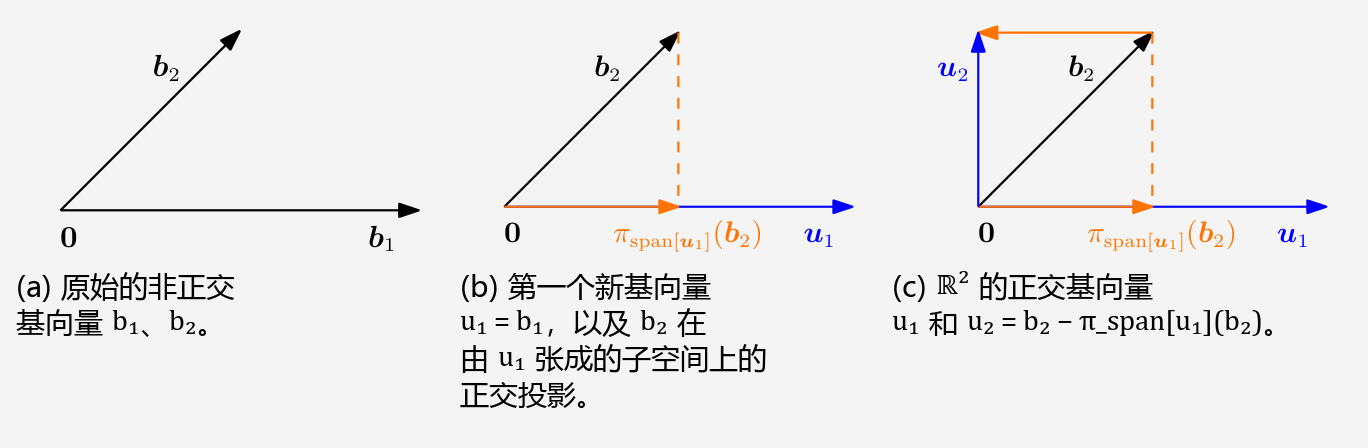
\includegraphics[width=0.92\textwidth,keepaspectratio]{docs/images/Figure3.12.png}
\caption*{\refstepcounter{figcounter}\label{fig:3-12}图~\thefigcounter 格拉姆-施密特正交化。(a) ℝ² 的非正交基 (b₁, b₂)；(b) 第一个构造的基向量 u₁ 以及 b₂ 在 span[u₁] 上的正交投影；(c) ℝ² 的正交基 (u₁, u₂)。}
\end{figure}


\section*{3.8.4 投影到仿射子空间}
\addcontentsline{toc}{subsection}{3.8.4 投影到仿射子空间}

到目前为止，我们讨论了如何将向量投影到低维子空间 $ U $ 上。接下来，我们给出将向量投影到 \emph{仿射子空间（affine subspace）} 的解决方案。

考虑图~\ref{fig:3-13}(a) 中的设定。给定一个仿射空间 $ L = \boldsymbol{x}_0 + U $，其中 $ \boldsymbol{b}_1, \boldsymbol{b}_2 $ 是 $ U $ 的基向量。为了确定 $ \boldsymbol{x} $ 在 $ L $ 上的正交投影 $ \pi_L(\boldsymbol{x}) $，我们将该问题转化为我们已知如何解决的问题：投影到向量子空间。为了实现这一点，我们从 $ \boldsymbol{x} $ 和 $ L $ 中减去支撑点 $ \boldsymbol{x}_0 $，使得 $ L - \boldsymbol{x}_0 = U $ 恰好是向量子空间 $ U $。现在我们可以使用第 3.8.2 节中讨论的子空间正交投影，得到投影 $ \pi_U(\boldsymbol{x} - \boldsymbol{x}_0) $，如图~\ref{fig:3-13}(b) 所示。现在可以通过加上 $ \boldsymbol{x}_0 $ 将此投影平移回 $ L $ 中，从而得到在仿射空间 $ L $ 上的正交投影：

\begin{equation}
\pi_L(\boldsymbol{x}) = \boldsymbol{x}_0 + \pi_U(\boldsymbol{x} - \boldsymbol{x}_0)
\tag{3.72}\label{eq:3-72}
\end{equation}

其中 $ \pi_U(\cdot) $ 是在子空间 $ U $（即 $ L $ 的方向空间）上的正交投影；参见图~\ref{fig:3-13}(c)。


\begin{figure}[H]
\centering
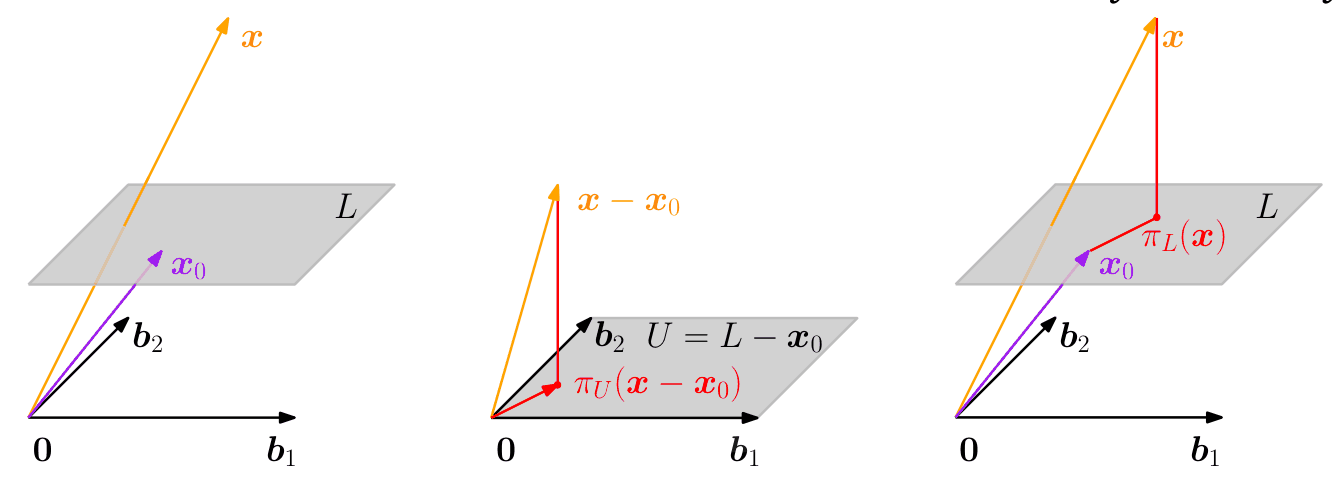
\includegraphics[width=0.92\textwidth,keepaspectratio]{docs/images/Figure3.13.png}
\caption*{\refstepcounter{figcounter}\label{fig:3-13}图~\thefigcounter 投影到仿射空间。(a) 原始设定；(b) 平移 −x₀ 使得 x − x₀ 可以投影到方向空间 U 上；(c) 将投影平移回 x₀ + πU(x − x₀)，得到最终的正交投影 πL(x)。}
\end{figure}


从图~\ref{fig:3-13} 中还可以明显看出，$ \boldsymbol{x} $ 到仿射空间 $ L $ 的距离与 $ \boldsymbol{x} - \boldsymbol{x}_0 $ 到 $ U $ 的距离相同，即：

\begin{equation}
d(\boldsymbol{x}, L) = \|\boldsymbol{x} - \pi_L(\boldsymbol{x})\| = \|\boldsymbol{x} - (\boldsymbol{x}_0 + \pi_U(\boldsymbol{x} - \boldsymbol{x}_0))\|
\tag{3.73a}\label{eq:3-73a}
\end{equation}

\begin{equation}
= d(\boldsymbol{x} - \boldsymbol{x}_0, \pi_U(\boldsymbol{x} - \boldsymbol{x}_0))
\tag{3.73b}\label{eq:3-73b}
\end{equation}

我们将在第 12.1 节中使用投影到仿射子空间的方法来推导分离超平面的概念。

\section*{3.9 旋转}
\addcontentsline{toc}{section}{3.9 旋转}
\label{sec:3.9}

正如在 3.4 节中所讨论的，保持长度和夹角不变是具有正交变换矩阵的线性映射的两个特征。接下来，我们将仔细研究描述旋转的特定正交变换矩阵。

一个 \emph{旋转（rotation）} 是一个线性映射（更具体地，是欧氏向量空间的一个自同构），它将平面绕原点旋转角度 $ \theta $，即原点是一个不动点。按照通用约定，对于正角 $ \theta > 0 $，我们按逆时针方向旋转。图~\ref{fig:3-14} 给出了一个示例，其中的变换矩阵为：

\begin{equation}
\boldsymbol{R} = \begin{bmatrix} -0.38 & -0.92 \\ 0.92 & -0.38 \end{bmatrix}
\tag{3.74}\label{eq:3-74}
\end{equation}


\begin{figure}[H]
\centering
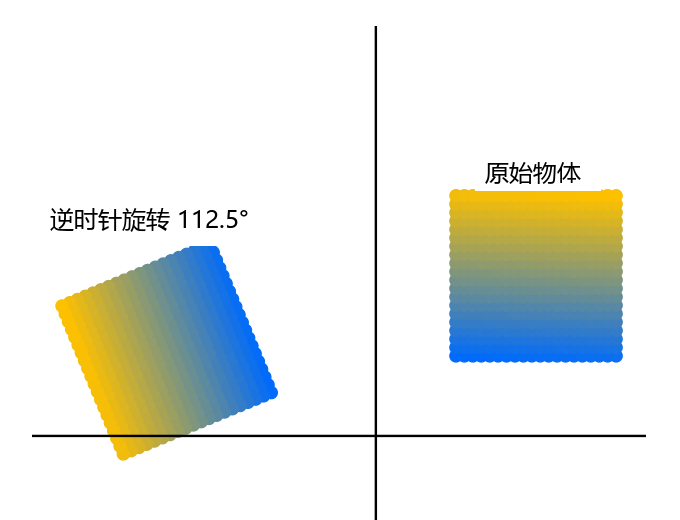
\includegraphics[width=0.92\textwidth,keepaspectratio]{docs/images/Figure3.14.png}
\caption*{\refstepcounter{figcounter}\label{fig:3-14}图~\thefigcounter 旋转将平面内的物体绕原点旋转。如果旋转角为正，则按逆时针方向旋转。}
\end{figure}


旋转的重要应用领域包括计算机图形学和机器人学。例如，在机器人学中，通常需要知道如何旋转机械臂的关节以便抓取或放置物体，参见图~\ref{fig:3-15}。


\begin{figure}[H]
\centering
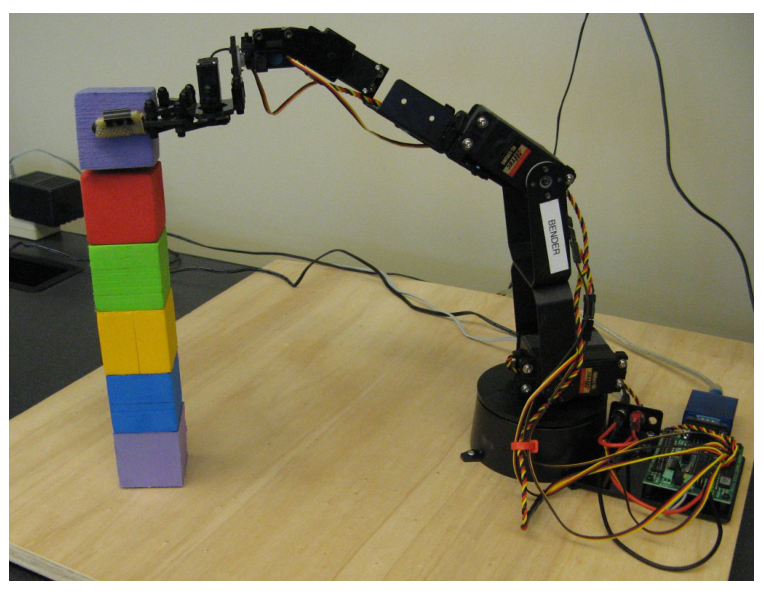
\includegraphics[width=0.92\textwidth,keepaspectratio]{docs/images/Figure3.15.png}
\caption*{\refstepcounter{figcounter}\label{fig:3-15}图~\thefigcounter 机械臂需要旋转其关节以便抓取或准确定位物体。图引自 (Deisenroth et al., 2015)。}
\end{figure}


\section*{3.9.1 $ \mathbb{R}^2 $ 中的旋转}
\addcontentsline{toc}{subsection}{3.9.1 $ \mathbb{R}^2 $ 中的旋转}

考虑 $ \mathbb{R}^2 $ 的标准基：

\begin{equation*}
\boldsymbol{e}_1 = \begin{bmatrix} 1 \\ 0 \end{bmatrix}, \quad \boldsymbol{e}_2 = \begin{bmatrix} 0 \\ 1 \end{bmatrix}
\end{equation*}

它定义了 $ \mathbb{R}^2 $ 中的标准坐标系。我们的目标是将该坐标系旋转角度 $ \theta $，如图~\ref{fig:3-16} 所示。注意，旋转后的向量仍然是线性无关的，因此它们构成了 $ \mathbb{R}^2 $ 的一组基。这意味着旋转执行了一次基变换。


\begin{figure}[H]
\centering
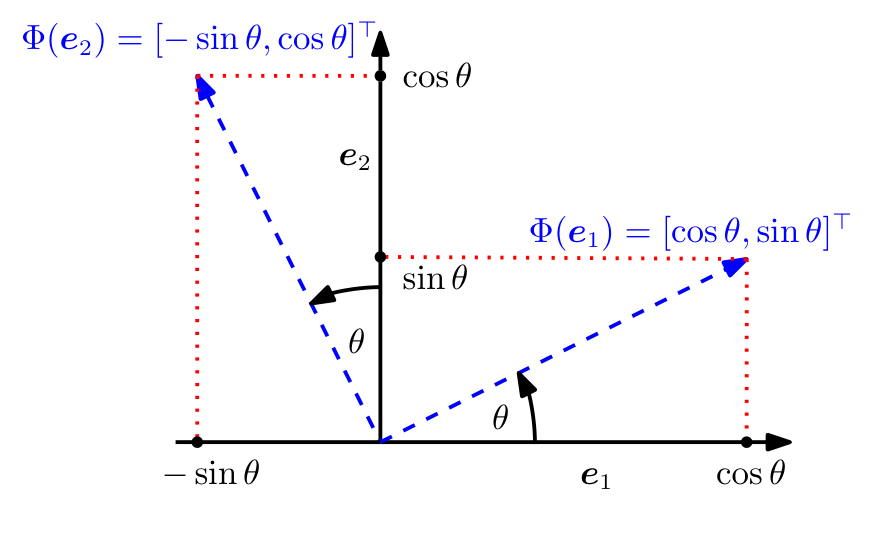
\includegraphics[width=0.92\textwidth,keepaspectratio]{docs/images/Figure3.16.png}
\caption*{\refstepcounter{figcounter}\label{fig:3-16}图~\thefigcounter R² 中的标准基旋转角度 θ。}
\end{figure}


旋转 $ \Phi $ 是线性映射，因此我们可以用一个 \emph{旋转矩阵（rotation matrix）} $ \boldsymbol{R}(\theta) $ 来表示它们。利用三角学知识（见图~\ref{fig:3-16}），我们可以确定旋转后的坐标轴（即 $ \Phi $ 的像）相对于 $ \mathbb{R}^2 $ 标准基的坐标。我们得到：

\begin{equation}
\Phi(\boldsymbol{e}_1) = \begin{bmatrix} \cos\theta \\ \sin\theta \end{bmatrix}, \quad \Phi(\boldsymbol{e}_2) = \begin{bmatrix} -\sin\theta \\ \cos\theta \end{bmatrix}
\tag{3.75}\label{eq:3-75}
\end{equation}

因此，执行到旋转后坐标的基变换矩阵 $ \boldsymbol{R}(\theta) $ 由下式给出：

\begin{equation}
\boldsymbol{R}(\theta) = \begin{bmatrix} \Phi(\boldsymbol{e}_1) & \Phi(\boldsymbol{e}_2) \end{bmatrix} = \begin{bmatrix} \cos\theta & -\sin\theta \\ \sin\theta & \cos\theta \end{bmatrix}
\tag{3.76}\label{eq:3-76}
\end{equation}

\section*{3.9.2 $ \mathbb{R}^3 $ 中的旋转}
\addcontentsline{toc}{subsection}{3.9.2 $ \mathbb{R}^3 $ 中的旋转}

与 $ \mathbb{R}^2 $ 的情形不同，在 $ \mathbb{R}^3 $ 中，我们可以将任意二维平面绕一维轴进行旋转。指定一般旋转矩阵的最简单方法是：指定标准基 $ \boldsymbol{e}_1, \boldsymbol{e}_2, \boldsymbol{e}_3 $ 的像应该如何旋转，并确保这些像 $ \boldsymbol{R} \boldsymbol{e}_1, \boldsymbol{R} \boldsymbol{e}_2, \boldsymbol{R} \boldsymbol{e}_3 $ 彼此相互标准正交。然后，我们可以通过组合标准基的像来得到一般的旋转矩阵 $ \boldsymbol{R} $。

为了使旋转角有明确的几何意义，当在高于两维的空间中操作时，我们必须明确“逆时针”的含义。我们采用如下约定：绕某个轴的“逆时针”（平面）旋转是指当我们从该轴的“末端正对轴向原点看去”时的旋转。因此，在 $ \mathbb{R}^3 $ 中，存在绕三个标准基向量的三个（平面）旋转（见图~\ref{fig:3-17}）：


\begin{figure}[H]
\centering
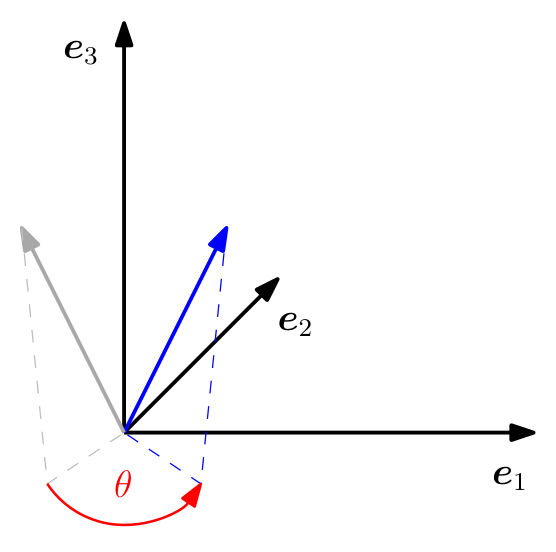
\includegraphics[width=320pt,keepaspectratio]{docs/images/Figure3.17.png}
\caption*{\refstepcounter{figcounter}\label{fig:3-17}图~\thefigcounter R³ 中的向量（灰色）绕 e₃ 轴旋转角度 θ。旋转后的向量显示为蓝色。}
\end{figure}


绕 $ \boldsymbol{e}_1 $ 轴旋转：

\begin{equation}
\begin{adjustbox}{max width=\linewidth}
\boldsymbol{R}_1(\theta) = \begin{bmatrix} \Phi(\boldsymbol{e}_1) & \Phi(\boldsymbol{e}_2) & \Phi(\boldsymbol{e}_3) \end{bmatrix} = \begin{bmatrix} 1 & 0 & 0 \\ 0 & \cos\theta & -\sin\theta \\ 0 & \sin\theta & \cos\theta \end{bmatrix}
\end{adjustbox}
\tag{3.77}\label{eq:3-77}
\end{equation}

在此处，$ \boldsymbol{e}_1 $ 坐标保持固定，逆时针旋转在 $ \boldsymbol{e}_2\boldsymbol{e}_3 $ 平面内进行。

绕 $ \boldsymbol{e}_2 $ 轴旋转：

\begin{equation}
\boldsymbol{R}_2(\theta) = \begin{bmatrix} \cos\theta & 0 & \sin\theta \\ 0 & 1 & 0 \\ -\sin\theta & 0 & \cos\theta \end{bmatrix}
\tag{3.78}\label{eq:3-78}
\end{equation}

如果我们绕 $ \boldsymbol{e}_2 $ 轴旋转 $ \boldsymbol{e}_1\boldsymbol{e}_3 $ 平面，我们需要从 $ \boldsymbol{e}_2 $ 轴的“尖端”朝向原点看去。

绕 $ \boldsymbol{e}_3 $ 轴旋转：

\begin{equation}
\boldsymbol{R}_3(\theta) = \begin{bmatrix} \cos\theta & -\sin\theta & 0 \\ \sin\theta & \cos\theta & 0 \\ 0 & 0 & 1 \end{bmatrix}
\tag{3.79}\label{eq:3-79}
\end{equation}

图~\ref{fig:3-17} 说明了这一旋转。

\section*{3.9.3 $ n $ 维空间中的旋转}
\addcontentsline{toc}{subsection}{3.9.3 $ n $ 维空间中的旋转}

将旋转从二维和三维推广到 $ n $ 维欧氏向量空间，可以直观地描述为：固定 $ n - 2 $ 个维度，并将旋转限制在 $ n $ 维空间中的一个二维平面内。正如在三维情形中一样，我们可以旋转任意平面（$ \mathbb{R}^n $ 的二维子空间）。

\textbf{定义 3.11}（吉文斯旋转）。设 $ V $ 为一个 $ n $ 维欧氏向量空间，$ \Phi: V \to V $ 为一个自同构，其变换矩阵为：

\begin{equation}
\begin{adjustbox}{max width=\linewidth}
\boldsymbol{R}_{ij}(\theta) := \begin{bmatrix} \boldsymbol{I}_{i-1} & \mathbf{0} & \cdots & \cdots & \mathbf{0} \\ \mathbf{0} & \cos\theta & \mathbf{0} & -\sin\theta & \mathbf{0} \\ \mathbf{0} & \mathbf{0} & \boldsymbol{I}_{j-i-1} & \mathbf{0} & \mathbf{0} \\ \mathbf{0} & \sin\theta & \mathbf{0} & \cos\theta & \mathbf{0} \\ \mathbf{0} & \cdots & \cdots & \mathbf{0} & \boldsymbol{I}_{n-j} \end{bmatrix} \in \mathbb{R}^{n \times n}
\end{adjustbox}
\tag{3.80}\label{eq:3-80}
\end{equation}

其中 $ 1 \leqslant i < j \leqslant n $ 且 $ \theta \in \mathbb{R} $。则称 $ \boldsymbol{R}_{ij}(\theta) $ 为一个 \emph{吉文斯旋转（Givens rotation）} 。

本质上，$ \boldsymbol{R}_{ij}(\theta) $ 是满足下列条件的单位矩阵 $ \boldsymbol{I}_n $：

\begin{equation}
r_{ii} = \cos\theta, \quad r_{ij} = -\sin\theta, \quad r_{ji} = \sin\theta, \quad r_{jj} = \cos\theta
\tag{3.81}\label{eq:3-81}
\end{equation}

在二维情况下（即 $ n = 2 $），我们得到式~\eqref{eq:3-76} 作为其特例。

\section*{3.9.4 旋转的性质}
\addcontentsline{toc}{subsection}{3.9.4 旋转的性质}

旋转表现出一系列有用的性质，这些性质可以通过将它们视为正交矩阵（定义 3.8）来推导得出：

\begin{itemize}
\item 旋转保持距离不变，即 $ \|\boldsymbol{x} - \boldsymbol{y}\| = \|\boldsymbol{R}_\theta(\boldsymbol{x}) - \boldsymbol{R}_\theta(\boldsymbol{y})\| $。换句话说，旋转变换后任意两点之间的距离保持不变。
\item 旋转保持夹角不变，即 $ \boldsymbol{R}_\theta \boldsymbol{x} $ 与 $ \boldsymbol{R}_\theta \boldsymbol{y} $ 之间的夹角等于 $ \boldsymbol{x} $ 与 $ \boldsymbol{y} $ 之间的夹角。
\item 三维（或更高维）中的旋转通常是不可交换的。因此，即使是绕同一个点旋转，应用旋转的顺序也是至关重要的。只有在二维空间中，向量旋转才是可交换的，即对于所有的 $ \phi, \theta \in [0, 2\pi) $，都有 $ \boldsymbol{R}(\phi)\boldsymbol{R}(\theta) = \boldsymbol{R}(\theta)\boldsymbol{R}(\phi) $。仅当它们绕同一个点（例如原点）旋转时，才在乘法运算下构成一个 \emph{阿贝尔群（Abelian group）} 。
\end{itemize}

\section*{3.10 延伸阅读}
\addcontentsline{toc}{section}{3.10 延伸阅读}
\label{sec:3.10}

在本章中，我们简要概述了解析几何的一些重要概念，这些概念将在本书后续各章中使用。若需对我们所介绍的概念进行更广泛和深入的了解，推荐阅读以下优秀教材：Axler (2015) 以及 Boyd and Vandenberghe (2018)。

内积使我们能够利用格拉姆-施密特方法（Gram-Schmidt method）确定向量（子）空间的特定基，其中每个向量都与其他所有向量正交（正交基）。这些基在优化以及求解线性方程组的数值算法中至关重要。例如，克雷洛夫子空间方法（Krylov subspace methods），如共轭梯度法（conjugate gradients）或广义极小残差法（generalized minimal residual method, GMRES），通过最小化彼此正交的残差误差来求解 (Stoer and Burlirsch, 2002)。

在机器学习中，内积在核方法（kernel methods）中尤为重要 (Schölkopf and Smola, 2002)。核方法利用了许多线性算法可以纯粹通过内积计算来表示这一事实。于是，“核技巧”（kernel trick）使我们能够在（可能是无限维的）特征空间中隐式地计算这些内积，甚至无需显式地知道该特征空间。这使得机器学习中使用的许多算法实现了“非线性化”，例如用于降维的核主成分分析（kernel-PCA）(Schölkopf et al., 1997)。高斯过程（Gaussian processes）(Rasmussen and Williams, 2006) 也属于核方法的范畴，是目前概率回归（数据点曲线拟合）领域的前沿方法。核方法的思想将在第 12 章中做进一步探讨。

投影常用于计算机图形学中，例如生成阴影。在优化中，正交投影常用于（迭代地）最小化残差误差。这在机器学习中同样有重要应用，例如在线性回归中，我们希望找到一个最小化残差误差的（线性）函数，即数据到该线性函数上的正交投影长度 (Bishop, 2006)。我们将在第 9 章对此进行更深入的研究。PCA (Pearson, 1901; Hotelling, 1933) 同样利用投影来降低高维数据的维度。我们将在第 10 章更详细地讨论这一点。

\chapter*{练习}
\addcontentsline{toc}{section}{练习}

\section*{练习 4.1}
\addcontentsline{toc}{subsection}{练习 4.1}

对于矩阵

\begin{equation*}
\boldsymbol{A} = \begin{bmatrix} 1 & 3 & 5 \\ 2 & 4 & 6 \\ 0 & 2 & 4 \end{bmatrix}
\end{equation*}

分别使用拉普拉斯展开（沿第一行）和萨鲁斯法则（Sarrus' rule）计算其行列式。

\medskip\hrule\medskip

\section*{练习 4.2}
\addcontentsline{toc}{subsection}{练习 4.2}

高效计算下列矩阵的行列式：

\begin{equation*}
\begin{adjustbox}{max width=\linewidth}
\begin{bmatrix} 2 & 0 & 1 & 2 & 0 \\ 2 & -1 & 0 & 1 & 1 \\ 0 & 1 & 2 & 1 & 2 \\ -2 & 0 & 2 & -1 & 2 \\ 2 & 0 & 0 & 1 & 1 \end{bmatrix}
\end{adjustbox}
\end{equation*}

\medskip\hrule\medskip

\section*{练习 4.3}
\addcontentsline{toc}{subsection}{练习 4.3}

计算下列矩阵的特征空间：

\begin{equation*}
\begin{bmatrix} 1 & 0 \\ 1 & 1 \end{bmatrix}, \quad \begin{bmatrix} -2 & 2 \\ 2 & 1 \end{bmatrix}
\end{equation*}

\medskip\hrule\medskip

\section*{练习 4.4}
\addcontentsline{toc}{subsection}{练习 4.4}

计算矩阵

\begin{equation*}
\begin{adjustbox}{max width=\linewidth}
\boldsymbol{A} = \begin{bmatrix} 0 & -1 & 1 & 1 \\ -1 & 1 & -2 & 3 \\ 2 & -1 & 0 & 0 \\ 1 & -1 & 1 & 0 \end{bmatrix}
\end{adjustbox}
\end{equation*}

的所有特征空间。

\medskip\hrule\medskip

\section*{练习 4.5}
\addcontentsline{toc}{subsection}{练习 4.5}

矩阵的可对角化性与其可逆性无关。判断下列四个矩阵是否可对角化和/或可逆：

\begin{equation*}
\begin{bmatrix} 1 & 0 \\ 0 & 1 \end{bmatrix}, \quad \begin{bmatrix} 1 & 0 \\ 0 & 0 \end{bmatrix}, \quad \begin{bmatrix} 1 & 1 \\ 0 & 1 \end{bmatrix}, \quad \begin{bmatrix} 0 & 1 \\ 0 & 0 \end{bmatrix}
\end{equation*}

\medskip\hrule\medskip

\section*{练习 4.6}
\addcontentsline{toc}{subsection}{练习 4.6}

计算下列变换矩阵的特征空间。它们可对角化吗？

a.

\begin{equation*}
\boldsymbol{A} = \begin{bmatrix} 2 & 3 & 0 \\ 1 & 4 & 3 \\ 0 & 0 & 1 \end{bmatrix}
\end{equation*}

b.

\begin{equation*}
\begin{adjustbox}{max width=\linewidth}
\boldsymbol{A} = \begin{bmatrix} 1 & 1 & 0 & 0 \\ 0 & 0 & 0 & 0 \\ 0 & 0 & 0 & 0 \\ 0 & 0 & 0 & 0 \end{bmatrix}
\end{adjustbox}
\end{equation*}

\medskip\hrule\medskip

\section*{练习 4.7}
\addcontentsline{toc}{subsection}{练习 4.7}

下列矩阵是否可对角化？若是，求其对角形式以及变换矩阵关于其呈对角形式的基。若否，给出它们不可对角化的理由。

a.

\begin{equation*}
\boldsymbol{A} = \begin{bmatrix} 0 & 1 \\ -8 & 4 \end{bmatrix}
\end{equation*}

b.

\begin{equation*}
\boldsymbol{A} = \begin{bmatrix} 1 & 1 & 1 \\ 1 & 1 & 1 \\ 1 & 1 & 1 \end{bmatrix}
\end{equation*}

c.

\begin{equation*}
\begin{adjustbox}{max width=\linewidth}
\boldsymbol{A} = \begin{bmatrix} 5 & 4 & 2 & 1 \\ 0 & 1 & -1 & -1 \\ -1 & -1 & 3 & 0 \\ 1 & 1 & -1 & 2 \end{bmatrix}
\end{adjustbox}
\end{equation*}

d.

\begin{equation*}
\boldsymbol{A} = \begin{bmatrix} 5 & -6 & -6 \\ -1 & 4 & 2 \\ 3 & -6 & -4 \end{bmatrix}
\end{equation*}

\medskip\hrule\medskip

\section*{练习 4.8}
\addcontentsline{toc}{subsection}{练习 4.8}

求矩阵

\begin{equation*}
\boldsymbol{A} = \begin{bmatrix} 3 & 2 & 2 \\ 2 & 3 & -2 \end{bmatrix}
\end{equation*}

的奇异值分解（SVD）。

\medskip\hrule\medskip

\section*{练习 4.9}
\addcontentsline{toc}{subsection}{练习 4.9}

求矩阵

\begin{equation*}
\boldsymbol{A} = \begin{bmatrix} 2 & 2 \\ -1 & 1 \end{bmatrix}
\end{equation*}

的奇异值分解。

\medskip\hrule\medskip

\section*{练习 4.10}
\addcontentsline{toc}{subsection}{练习 4.10}

求矩阵

\begin{equation*}
\boldsymbol{A} = \begin{bmatrix} 3 & 2 & 2 \\ 2 & 3 & -2 \end{bmatrix}
\end{equation*}

的最佳秩 1 近似。

\medskip\hrule\medskip

\section*{练习 4.11}
\addcontentsline{toc}{subsection}{练习 4.11}

证明：对于任意 $ \boldsymbol{A} \in \mathbb{R}^{m \times n} $，矩阵 $ \boldsymbol{A}^\top \boldsymbol{A} $ 与 $ \boldsymbol{A} \boldsymbol{A}^\top $ 具有相同的非零特征值。

\medskip\hrule\medskip

\section*{练习 4.12}
\addcontentsline{toc}{subsection}{练习 4.12}

证明对于 $ \boldsymbol{x} \neq \boldsymbol{0} $ 定理 4.24 成立，即证明：

\begin{equation*}
\max_{\boldsymbol{x}} \frac{\|\boldsymbol{A} \boldsymbol{x}\|_2}{\|\boldsymbol{x}\|_2} = \sigma_1
\end{equation*}

其中 $ \sigma_1 $ 是 $ \boldsymbol{A} \in \mathbb{R}^{m \times n} $ 的最大奇异值。

\chapter{4 矩阵分解}

在第 2 章和第 3 章中，我们研究了处理和度量向量、向量投影以及线性映射的方法。向量的映射与变换可以方便地描述为矩阵执行的运算。此外，数据通常也以矩阵形式表示，例如矩阵的行表示不同的人，而列描述这些人的不同特征（如体重、身高和社会经济地位等）。在本章中，我们将介绍矩阵的三个方面：如何概括矩阵、如何分解矩阵，以及如何将这些分解用于矩阵近似。

我们首先考虑仅用几个数字来刻画矩阵总体性质的方法。我们将在行列式（第 4.1 节）和特征值（第 4.2 节）中针对方阵这一重要特殊情形进行讨论。这些特征数字具有重要的数学意义，能让我们快速掌握矩阵具备哪些有用性质。在此基础上，我们将进一步讨论矩阵分解方法：矩阵分解的一个类比是数的因数分解，例如将 21 分解为质数 $ 7 \cdot 3 $。出于这个原因，矩阵分解通常也被称为 \emph{矩阵因子分解（matrix factorization）} 。矩阵分解旨在通过可解释矩阵的因子所构成的一种不同表示来描述矩阵。

我们将首先讨论对称正定矩阵的一种类似于“开方”的运算：Cholesky 分解（第 4.3 节）。随后，我们将介绍将矩阵分解为规范形式的两种相关方法。第一种称为矩阵对角化（第 4.4 节），如果选择适当的基，它允许我们使用对角变换矩阵来表示线性映射。第二种方法是奇异值分解（SVD，第 4.5 节），它将该分解推广到了非方阵情形，被认为是线性代数中最基础的概念之一。这些分解非常有用，因为表示数值数据的矩阵通常非常庞大且难以直接分析。最后，我们将以矩阵分类体系（第 4.7 节）的形式系统概述矩阵的类型及其区分特征，以总结全章。

我们在本章介绍的方法不仅在后续的数学章节（例如第 6 章）中发挥重要作用，而且在应用章节中同样不可或缺，例如第 10 章的降维和第 11 章的密度估计。本章的总体结构如图~\ref{fig:4-1} 的思维导图所示。


\begin{figure}[H]
\centering
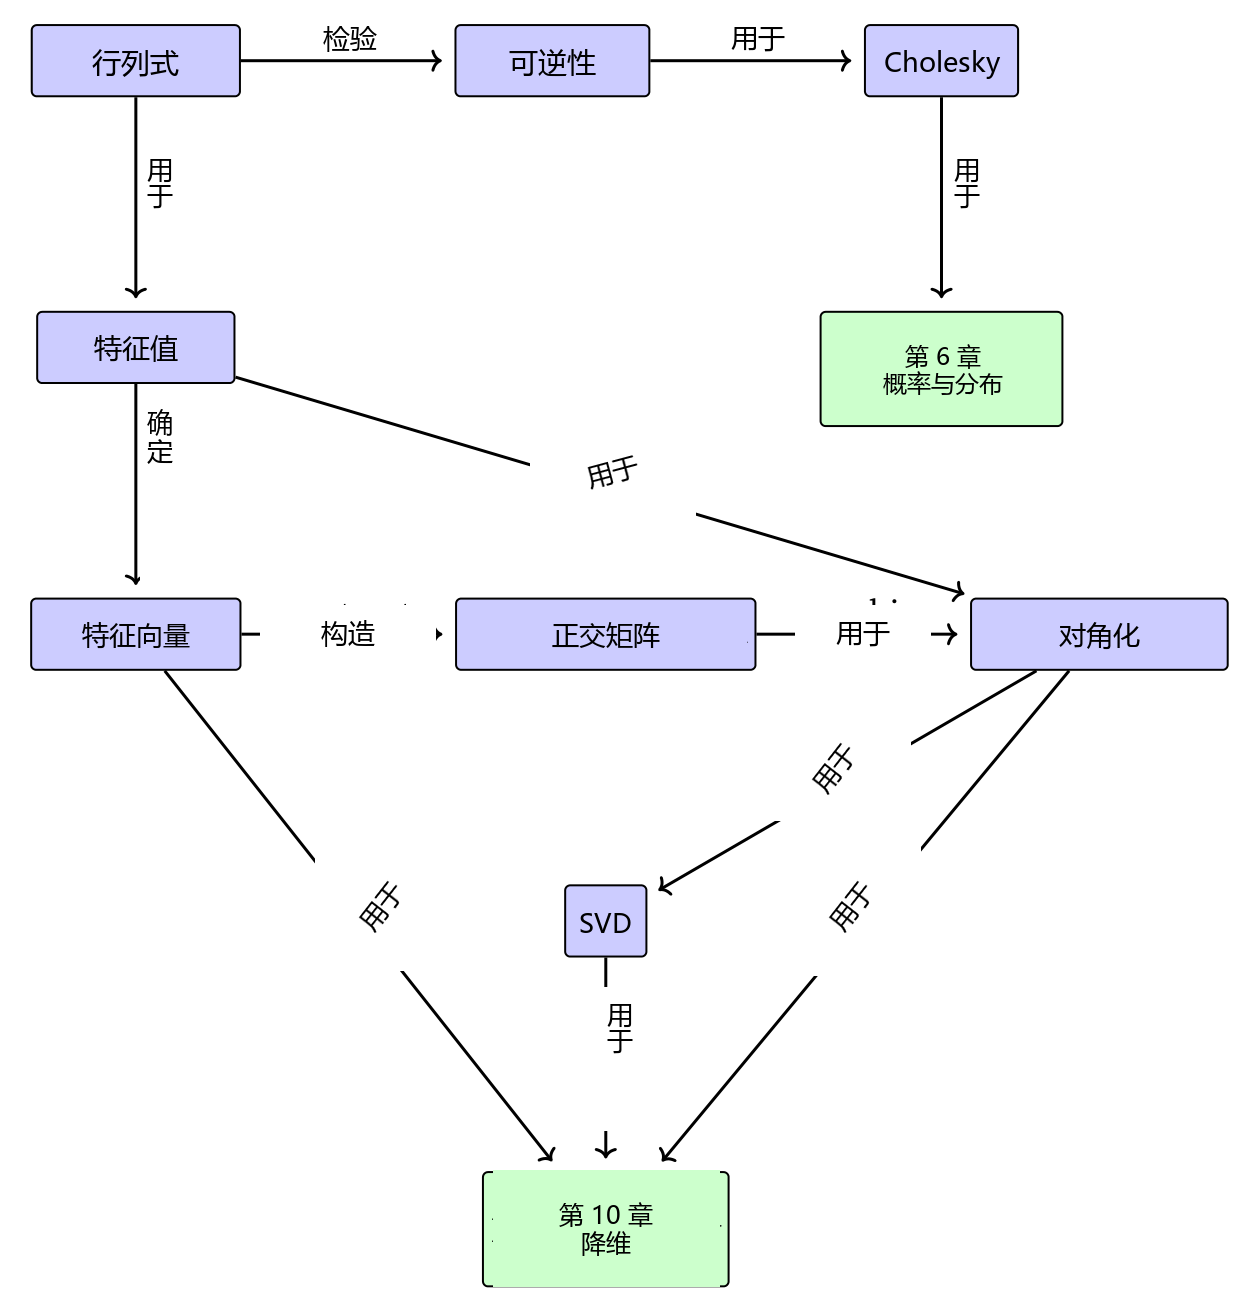
\includegraphics[width=320pt,keepaspectratio]{docs/images/Figure4.1.png}
\caption*{\refstepcounter{figcounter}\label{fig:4-1}图~\thefigcounter 本章介绍的概念的思维导图，以及它们在本书其他部分中的应用场景。}
\end{figure}


\section*{4.1 行列式与迹}
\addcontentsline{toc}{section}{4.1 行列式与迹}
\label{sec:4.1}

行列式是线性代数中的重要概念。行列式是线性方程组分析与求解中的一种数学对象。行列式仅对方阵 $ \boldsymbol{A} \in \mathbb{R}^{n \times n} $（即行数与列数相等的矩阵）有定义。在本书中，我们将行列式记为 $ \det(\boldsymbol{A}) $，有时也记作 $ |\boldsymbol{A}| $，因此：

\begin{equation}
\begin{adjustbox}{max width=\linewidth}
\det(\boldsymbol{A}) = \begin{vmatrix} a_{11} & a_{12} & \cdots & a_{1n} \\ a_{21} & a_{22} & \cdots & a_{2n} \\ \vdots & \vdots & \ddots & \vdots \\ a_{n1} & a_{n2} & \cdots & a_{nn} \end{vmatrix}
\end{adjustbox}
\tag{4.1}\label{eq:4-1}
\end{equation}

\emph{备注} 。行列式记号 $ |\boldsymbol{A}| $ 切勿与绝对值混淆。♦

方阵 $ \boldsymbol{A} \in \mathbb{R}^{n \times n} $ 的 \emph{行列式（determinant）} 是一个将 $ \boldsymbol{A} $ 映射到实数的函数。在给出一般 $ n \times n $ 矩阵的行列式定义之前，我们先来看一些具有启发性的示例，并定义一些特殊矩阵的行列式。

\begin{notebox}
\textbf{例 4.1（检验矩阵的可逆性）}
\end{notebox}

\begin{notebox}
我们首先探讨方阵 $ \boldsymbol{A} $ 是否可逆（参见第 2.2.2 节）。对于最小维度的情形，我们已经知道矩阵何时可逆。如果 $ \boldsymbol{A} $ 是 $ 1 \times 1 $ 矩阵（即一个标量），那么 $ \boldsymbol{A} = a \implies \boldsymbol{A}^{-1} = \frac{1}{a} $。因此，$ a \cdot \frac{1}{a} = 1 $ 成立当且仅当 $ a \neq 0 $。
\end{notebox}

\begin{notebox}
对于 $ 2 \times 2 $ 矩阵，由逆矩阵的定义（定义 2.3），我们知道 $ \boldsymbol{A} \boldsymbol{A}^{-1} = \boldsymbol{I} $。结合式~\eqref{eq:2-24}，$ \boldsymbol{A} $ 的逆矩阵为：

\begin{equation}
\boldsymbol{A}^{-1} = \frac{1}{a_{11}a_{22} - a_{12}a_{21}} \begin{bmatrix} a_{22} & -a_{12} \\ -a_{21} & a_{11} \end{bmatrix}
\tag{4.2}\label{eq:4-2}
\end{equation}

因此，$ \boldsymbol{A} $ 可逆当且仅当：

\begin{equation}
a_{11}a_{22} - a_{12}a_{21} \neq 0
\tag{4.3}\label{eq:4-3}
\end{equation}

该量即为 $ \boldsymbol{A} \in \mathbb{R}^{2 \times 2} $ 的行列式，即：

\begin{equation}
\det(\boldsymbol{A}) = \begin{vmatrix} a_{11} & a_{12} \\ a_{21} & a_{22} \end{vmatrix} = a_{11}a_{22} - a_{12}a_{21}
\tag{4.4}\label{eq:4-4}
\end{equation}
\end{notebox}

例 4.1 已经指出了行列式与逆矩阵存在性之间的关系。下面的定理将这一结论推广到一般 $ n \times n $ 矩阵。

\textbf{定理 4.1}。对于任意方阵 $ \boldsymbol{A} \in \mathbb{R}^{n \times n} $，$ \boldsymbol{A} $ 可逆当且仅当 $ \det(\boldsymbol{A}) \neq 0 $。

对于小型矩阵，我们可以根据矩阵元素给出行列式的显式（闭式）表达式。对于 $ n = 1 $：

\begin{equation}
\det(\boldsymbol{A}) = \det(a_{11}) = a_{11}
\tag{4.5}\label{eq:4-5}
\end{equation}

对于 $ n = 2 $：

\begin{equation}
\det(\boldsymbol{A}) = \begin{vmatrix} a_{11} & a_{12} \\ a_{21} & a_{22} \end{vmatrix} = a_{11}a_{22} - a_{12}a_{21}
\tag{4.6}\label{eq:4-6}
\end{equation}

这正是我们在前一个示例中观察到的结果。

对于 $ n = 3 $，对应的计算法则称为 \emph{萨鲁斯法则（Sarrus' rule）} ：

\begin{equation}
\begin{adjustbox}{max width=\linewidth}
\begin{vmatrix} a_{11} & a_{12} & a_{13} \\ a_{21} & a_{22} & a_{23} \\ a_{31} & a_{32} & a_{33} \end{vmatrix} = a_{11}a_{22}a_{33} + a_{21}a_{32}a_{13} + a_{31}a_{12}a_{23} - a_{31}a_{22}a_{13} - a_{11}a_{32}a_{23} - a_{21}a_{12}a_{33}
\end{adjustbox}
\tag{4.7}\label{eq:4-7}
\end{equation}

为了便于记忆萨鲁斯法则中的乘积项，可以尝试在矩阵中画出对角线乘积元素。

如果方阵 $ \boldsymbol{T} $ 满足当 $ i > j $ 时 $ T_{ij} = 0 $（即主对角线下方元素全为 0），我们称其为 \emph{上三角矩阵（upper-triangular matrix）} 。类似地，如果主对角线上方元素全为 0，我们定义其为 \emph{下三角矩阵（lower-triangular matrix）} 。对于三角矩阵 $ \boldsymbol{T} \in \mathbb{R}^{n \times n} $，其行列式是对角线元素的乘积，即：

\begin{equation}
\det(\boldsymbol{T}) = \prod_{i=1}^n T_{ii}
\tag{4.8}\label{eq:4-8}
\end{equation}


\begin{figure}[H]
\centering
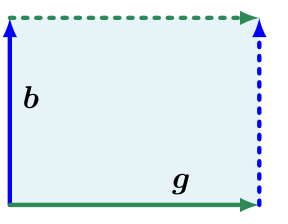
\includegraphics[width=0.92\textwidth,keepaspectratio]{docs/images/Figure4.2.png}
\caption*{\refstepcounter{figcounter}\label{fig:4-2}图~\thefigcounter 由向量 b 和 g 张成的平行四边形（阴影区域）面积为 |det([b, g])|。}
\end{figure}



\begin{figure}[H]
\centering
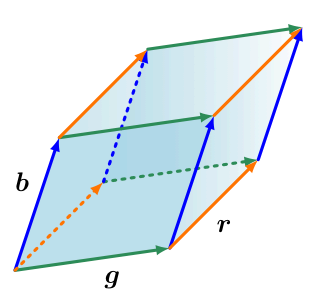
\includegraphics[width=0.92\textwidth,keepaspectratio]{docs/images/Figure4.3.png}
\caption*{\refstepcounter{figcounter}\label{fig:4-3}图~\thefigcounter 由向量 r, b, g 张成的平行六面体（阴影体积）体积为 |det([r, b, g])|。}
\end{figure}


\begin{notebox}
\textbf{例 4.2（行列式作为体积的度量）}
\end{notebox}

\begin{notebox}
当我们将行列式视为从张成 $ \mathbb{R}^n $ 中几何对象的 $ n $ 个向量集合出发的映射时，行列式的概念是非常自然的。事实表明，行列式 $ \det(\boldsymbol{A}) $ 是由矩阵 $ \boldsymbol{A} $ 的列向量构成的 $ n $ 维平行多面体的 \emph{有向体积（signed volume）} 。
\end{notebox}

\begin{notebox}
对于 $ n = 2 $，矩阵的列向量构成一个平行四边形；参见图~\ref{fig:4-2}。随着向量之间的夹角变小，平行四边形的面积也会缩小。考虑构成矩阵 $ \boldsymbol{A} = [\boldsymbol{b}, \boldsymbol{g}] $ 列向量的两个向量 $ \boldsymbol{b}, \boldsymbol{g} $。那么，$ \boldsymbol{A} $ 的行列式绝对值等于以 $ \boldsymbol{0}, \boldsymbol{b}, \boldsymbol{g}, \boldsymbol{b} + \boldsymbol{g} $ 为顶点的平行四边形的面积。特别地，如果 $ \boldsymbol{b}, \boldsymbol{g} $ 线性相关（即对某个 $ \lambda \in \mathbb{R} $ 有 $ \boldsymbol{b} = \lambda \boldsymbol{g} $），它们便不再构成二维平行四边形，因此对应面积为 0。相反，若 $ \boldsymbol{b}, \boldsymbol{g} $ 线性无关且是标准基向量 $ \boldsymbol{e}_1, \boldsymbol{e}_2 $ 的倍数，则它们可以写为

\begin{equation*}
\boldsymbol{b} = \begin{bmatrix} b \\ 0 \end{bmatrix}
\end{equation*}

和

\begin{equation*}
\boldsymbol{g} = \begin{bmatrix} 0 \\ g \end{bmatrix}
\end{equation*}

，行列式为：

\begin{equation*}
\begin{vmatrix} b & 0 \\ 0 & g \end{vmatrix} = bg - 0 = bg
\end{equation*}

行列式的符号表示张成向量 $ \boldsymbol{b}, \boldsymbol{g} $ 相对于标准基 $ (\boldsymbol{e}_1, \boldsymbol{e}_2) $ 的 \emph{定向（orientation）} 。在图~\ref{fig:4-2} 中，若将顺序翻转为 $ \boldsymbol{g}, \boldsymbol{b} $，则交换了 $ \boldsymbol{A} $ 的列，并反转了阴影区域的定向。这就转化为了我们熟悉的公式：$ \textcn{面积} = \textcn{底} \times \textcn{高} $。
\end{notebox}

\begin{notebox}
这种直觉可以推广到更高维度。在 $ \mathbb{R}^3 $ 中，考虑三个向量 $ \boldsymbol{r}, \boldsymbol{b}, \boldsymbol{g} \in \mathbb{R}^3 $ 张成平行六面体的棱，即各个面均为平行四边形的多面体（参见图~\ref{fig:4-3}）。$ 3 \times 3 $ 矩阵 $ [\boldsymbol{r}, \boldsymbol{b}, \boldsymbol{g}] $ 行列式的绝对值就是该立体的体积。因此，行列式充当了度量由矩阵各列向量组合构成的有向体积的函数。
\end{notebox}

\begin{notebox}
考虑如下给出的三个线性无关向量 $ \boldsymbol{r}, \boldsymbol{g}, \boldsymbol{b} \in \mathbb{R}^3 $：

\begin{equation}
\boldsymbol{r} = \begin{bmatrix} 2 \\ 0 \\ -8 \end{bmatrix}, \quad \boldsymbol{g} = \begin{bmatrix} 6 \\ 1 \\ 0 \end{bmatrix}, \quad \boldsymbol{b} = \begin{bmatrix} 1 \\ 4 \\ -1 \end{bmatrix}
\tag{4.9}\label{eq:4-9}
\end{equation}

将这些向量写为矩阵的列：

\begin{equation}
\boldsymbol{A} = [\boldsymbol{r}, \boldsymbol{g}, \boldsymbol{b}] = \begin{bmatrix} 2 & 6 & 1 \\ 0 & 1 & 4 \\ -8 & 0 & -1 \end{bmatrix}
\tag{4.10}\label{eq:4-10}
\end{equation}

这允许我们计算所需的体积：

\begin{equation}
V = |\det(\boldsymbol{A})| = 186
\tag{4.11}\label{eq:4-11}
\end{equation}
\end{notebox}

计算 $ n \times n $ 矩阵的行列式需要一般的算法来求解 $ n > 3 $ 的情形，我们将在下文中进行探讨。下面的定理 4.2 将计算 $ n \times n $ 矩阵行列式的问题归结为计算 $ (n - 1) \times (n - 1) $ 矩阵的行列式。通过递归应用拉普拉斯展开（定理 4.2），我们可以通过最终计算 $ 2 \times 2 $ 矩阵的行列式来计算任意 $ n \times n $ 矩阵的行列式。

\textbf{定理 4.2}（拉普拉斯展开 / Laplace Expansion）。考虑矩阵 $ \boldsymbol{A} \in \mathbb{R}^{n \times n} $。那么对于所有的 $ j = 1, \ldots, n $：

\begin{enumerate}
\item 沿第 $ j $ 列展开：
\end{enumerate}

\begin{equation}
\det(\boldsymbol{A}) = \sum_{k=1}^n (-1)^{k+j} a_{kj} \det(\boldsymbol{A}_{k,j})
\tag{4.12}\label{eq:4-12}
\end{equation}

\begin{enumerate}
\item 沿第 $ j $ 行展开：
\end{enumerate}

\begin{equation}
\det(\boldsymbol{A}) = \sum_{k=1}^n (-1)^{k+j} a_{jk} \det(\boldsymbol{A}_{j,k})
\tag{4.13}\label{eq:4-13}
\end{equation}

这里 $ \boldsymbol{A}_{k,j} \in \mathbb{R}^{(n-1) \times (n-1)} $ 是从 $ \boldsymbol{A} $ 中划去第 $ k $ 行与第 $ j $ 列后得到的子矩阵。$ \det(\boldsymbol{A}_{k,j}) $ 称为 \emph{余子式（minor）} ，而 $ (-1)^{k+j}\det(\boldsymbol{A}_{k,j}) $ 称为 \emph{代数余子式（cofactor）} 。

\begin{notebox}
\textbf{例 4.3（拉普拉斯展开）}
\end{notebox}

\begin{notebox}
我们使用沿第一行的拉普拉斯展开来计算矩阵：

\begin{equation}
\boldsymbol{A} = \begin{bmatrix} 1 & 2 & 3 \\ 3 & 1 & 2 \\ 0 & 0 & 1 \end{bmatrix}
\tag{4.14}\label{eq:4-14}
\end{equation}

的行列式。应用式~\eqref{eq:4-13} 得到：

\begin{equation}
\begin{adjustbox}{max width=\linewidth}
\begin{vmatrix} 1 & 2 & 3 \\ 3 & 1 & 2 \\ 0 & 0 & 1 \end{vmatrix} = (-1)^{1+1} \cdot 1 \begin{vmatrix} 1 & 2 \\ 0 & 1 \end{vmatrix} + (-1)^{1+2} \cdot 2 \begin{vmatrix} 3 & 2 \\ 0 & 1 \end{vmatrix} + (-1)^{1+3} \cdot 3 \begin{vmatrix} 3 & 1 \\ 0 & 0 \end{vmatrix}
\end{adjustbox}
\tag{4.15}\label{eq:4-15}
\end{equation}

利用式~\eqref{eq:4-6} 计算所有 $ 2 \times 2 $ 矩阵的行列式，得到：

\begin{equation}
\det(\boldsymbol{A}) = 1(1 - 0) - 2(3 - 0) + 3(0 - 0) = -5
\tag{4.16}\label{eq:4-16}
\end{equation}

为了完整起见，我们可以将此结果与利用萨鲁斯法则 (4.7) 计算的结果进行比对：

\begin{equation}
\det(\boldsymbol{A}) = 1 \cdot 1 \cdot 1 + 3 \cdot 0 \cdot 3 + 0 \cdot 2 \cdot 2 - 0 \cdot 1 \cdot 3 - 1 \cdot 0 \cdot 2 - 3 \cdot 2 \cdot 1 = 1 - 6 = -5
\tag{4.17}\label{eq:4-17}
\end{equation}
\end{notebox}

对于 $ \boldsymbol{A} \in \mathbb{R}^{n \times n} $，行列式具备以下性质：

\begin{itemize}
\item 矩阵乘积的行列式等于对应行列式的乘积：$ \det(\boldsymbol{A} \boldsymbol{B}) = \det(\boldsymbol{A})\det(\boldsymbol{B}) $。
\item 行列式关于转置不变，即 $ \det(\boldsymbol{A}) = \det(\boldsymbol{A}^\top) $。
\item 若 $ \boldsymbol{A} $ 正则（可逆），则 $ \det(\boldsymbol{A}^{-1}) = \frac{1}{\det(\boldsymbol{A})} $。
\item 相似矩阵（定义 2.22）拥有相同的行列式。因此，对于线性映射 $ \Phi : V \to V $，$ \Phi $ 的所有变换矩阵 $ \boldsymbol{A}_\Phi $ 具有相同的行列式。换言之，行列式与线性映射基的选择无关。
\item 将某一列/行乘上标量后加到另一列/行，不改变 $ \det(\boldsymbol{A}) $。
\item 将某一列/行乘以 $ \lambda \in \mathbb{R} $，使得 $ \det(\boldsymbol{A}) $ 缩放 $ \lambda $ 倍。特别地，$ \det(\lambda \boldsymbol{A}) = \lambda^n \det(\boldsymbol{A}) $。
\item 交换两行/列会改变 $ \det(\boldsymbol{A}) $ 的符号。
\end{itemize}

由于最后三条性质，我们可以使用高斯消元法（参见第 2.1 节）将 $ \boldsymbol{A} $ 化为行阶梯形来计算 $ \det(\boldsymbol{A}) $。当我们将 $ \boldsymbol{A} $ 化为对角线下方全为 0 的三角形式时，便可终止高斯消元。回顾式~\eqref{eq:4-8}，三角矩阵的行列式等于对角线元素的乘积。

\textbf{定理 4.3}。方阵 $ \boldsymbol{A} \in \mathbb{R}^{n \times n} $ 满足 $ \det(\boldsymbol{A}) \neq 0 $ 当且仅当 $ \operatorname{rk}(\boldsymbol{A}) = n $。换言之，$ \boldsymbol{A} $ 可逆当且仅当它是满秩的。

在数学主要依靠手工计算的时代，计算行列式被认为是分析矩阵可逆性的重要途径。然而，现代机器学习方法使用直接数值方法取代了显式行列式计算。例如在第 2 章中，我们学习了逆矩阵可以通过高斯消元法计算。因此，高斯消元法同样可用于计算矩阵的行列式。

行列式在后续章节中具有重要的理论作用，尤其是当我们通过特征多项式学习特征值和特征向量（第 4.2 节）时。

\medskip\hrule\medskip

\section*{4.1.1 迹}
\addcontentsline{toc}{subsection}{4.1.1 迹}

\textbf{定义 4.4}（迹）。方阵 $ \boldsymbol{A} \in \mathbb{R}^{n \times n} $ 的 \emph{迹（trace）} 定义为：

\begin{equation}
\operatorname{tr}(\boldsymbol{A}) := \sum_{i=1}^n a_{ii}
\tag{4.18}\label{eq:4-18}
\end{equation}

即迹是 $ \boldsymbol{A} $ 主对角线上各元素的和。

迹满足以下性质：

\begin{itemize}
\item 对于 $ \boldsymbol{A}, \boldsymbol{B} \in \mathbb{R}^{n \times n} $：$ \operatorname{tr}(\boldsymbol{A} + \boldsymbol{B}) = \operatorname{tr}(\boldsymbol{A}) + \operatorname{tr}(\boldsymbol{B}) $
\item 对于 $ \alpha \in \mathbb{R}, \boldsymbol{A} \in \mathbb{R}^{n \times n} $：$ \operatorname{tr}(\alpha \boldsymbol{A}) = \alpha \operatorname{tr}(\boldsymbol{A}) $
\item $ \operatorname{tr}(\boldsymbol{I}_n) = n $
\item 对于 $ \boldsymbol{A} \in \mathbb{R}^{n \times k}, \boldsymbol{B} \in \mathbb{R}^{k \times n} $：$ \operatorname{tr}(\boldsymbol{A} \boldsymbol{B}) = \operatorname{tr}(\boldsymbol{B} \boldsymbol{A}) $
\end{itemize}

可以证明，同时满足这四个性质的函数是唯一的——即迹函数（Gohberg et al., 2012）。

矩阵乘积的迹具有更一般的性质。特别地，迹在循环排列下保持不变，即：

\begin{equation}
\operatorname{tr}(\boldsymbol{A} \boldsymbol{K} \boldsymbol{L}) = \operatorname{tr}(\boldsymbol{K} \boldsymbol{L} \boldsymbol{A})
\tag{4.19}\label{eq:4-19}
\end{equation}

其中 $ \boldsymbol{A} \in \mathbb{R}^{a \times k}, \boldsymbol{K} \in \mathbb{R}^{k \times l}, \boldsymbol{L} \in \mathbb{R}^{l \times a} $。该性质可推广至任意多个矩阵的乘积。作为式~\eqref{eq:4-19} 的特例，对于两个向量 $ \boldsymbol{x}, \boldsymbol{y} \in \mathbb{R}^n $，有：

\begin{equation}
\operatorname{tr}(\boldsymbol{x} \boldsymbol{y}^\top) = \operatorname{tr}(\boldsymbol{y}^\top \boldsymbol{x}) = \boldsymbol{y}^\top \boldsymbol{x} \in \mathbb{R}
\tag{4.20}\label{eq:4-20}
\end{equation}

给定向量空间 $ V $ 上的线性映射 $ \Phi : V \to V $，我们利用 $ \Phi $ 的矩阵表示的迹来定义该映射的迹。对于 $ V $ 的一组给定基，我们可以通过变换矩阵 $ \boldsymbol{A} $ 描述 $ \Phi $，那么 $ \Phi $ 的迹就是 $ \boldsymbol{A} $ 的迹。对于 $ V $ 的另一组基，对应的变换矩阵 $ \boldsymbol{B} $ 可以通过形如 $ \boldsymbol{S}^{-1}\boldsymbol{A}\boldsymbol{S} $ 的基变换获得（对于某个适当的 $ \boldsymbol{S} $，参见第 2.7.2 节）。对于 $ \Phi $ 对应的迹，这意味着：

\begin{equation}
\operatorname{tr}(\boldsymbol{B}) = \operatorname{tr}(\boldsymbol{S}^{-1}\boldsymbol{A}\boldsymbol{S}) = \operatorname{tr}(\boldsymbol{A}\boldsymbol{S}\boldsymbol{S}^{-1}) = \operatorname{tr}(\boldsymbol{A})
\tag{4.21}\label{eq:4-21}
\end{equation}

因此，尽管线性映射的矩阵表示依赖于基的选择，但线性映射 $ \Phi $ 的迹与基的选择无关。

\medskip\hrule\medskip

\section*{4.1.2 特征多项式}
\addcontentsline{toc}{subsection}{4.1.2 特征多项式}

在本节中，我们介绍了作为刻画方阵函数的行列式与迹。综合我们对行列式与迹的理解，我们现在可以定义一个用多项式描述矩阵 $ \boldsymbol{A} $ 的重要方程，我们将在后续小节中广泛使用它。

\textbf{定义 4.5}（特征多项式）。对于 $ \lambda \in \mathbb{R} $ 和方阵 $ \boldsymbol{A} \in \mathbb{R}^{n \times n} $：

\begin{equation}
p_{\boldsymbol{A}}(\lambda) := \det(\boldsymbol{A} - \lambda \boldsymbol{I})
\tag{4.22a}\label{eq:4-22a}
\end{equation}

\begin{equation}
= c_0 + c_1\lambda + c_2\lambda^2 + \cdots + c_{n-1}\lambda^{n-1} + (-1)^n\lambda^n
\tag{4.22b}\label{eq:4-22b}
\end{equation}

（其中 $ c_0, \ldots, c_{n-1} \in \mathbb{R} $）称为 $ \boldsymbol{A} $ 的 \emph{特征多项式（characteristic polynomial）} 。特别地：

\begin{equation}
c_0 = \det(\boldsymbol{A})
\tag{4.23}\label{eq:4-23}
\end{equation}

\begin{equation}
c_{n-1} = (-1)^{n-1}\operatorname{tr}(\boldsymbol{A})
\tag{4.24}\label{eq:4-24}
\end{equation}

特征多项式~\eqref{eq:4-22a} 将允许我们计算特征值和特征向量，我们将在下一节中进行讨论。

\section*{4.2 特征值与特征向量}
\addcontentsline{toc}{section}{4.2 特征值与特征向量}
\label{sec:4.2}

现在我们将了解一种表征矩阵及其相关线性映射的新方法。回顾第 2.7.1 节，在给定有序基的情况下，每个线性映射都有一个唯一的变换矩阵。我们可以通过进行“特征（eigen）”分析来解释线性映射及其相关的变换矩阵（“eigen”是一个德语词，意为“特征的”、“自身的”或“特有的”）。正如我们将看到的，线性映射的特征值将告诉我们一组特殊的向量——特征向量——是如何被该线性映射变换的。

\textbf{定义 4.6}（特征值与特征向量）。设 $ \boldsymbol{A} \in \mathbb{R}^{n \times n} $ 为方阵。若满足：

\begin{equation}
\boldsymbol{A} \boldsymbol{x} = \lambda \boldsymbol{x}
\tag{4.25}\label{eq:4-25}
\end{equation}

则称 $ \lambda \in \mathbb{R} $ 为 $ \boldsymbol{A} $ 的一个 \emph{特征值（eigenvalue）} ，$ \boldsymbol{x} \in \mathbb{R}^n \setminus \{\boldsymbol{0}\} $ 为 $ \boldsymbol{A} $ 对应于 $ \lambda $ 的 \emph{特征向量（eigenvector）} 。我们称式~\eqref{eq:4-25} 为 \emph{特征值方程（eigenvalue equation）} 。

\emph{备注} 。在线性代数文献和软件中，通常的惯例是将特征值按降序排列，使得最大的特征值及相关特征向量称为第一特征值及其相关特征向量，次大的特征值称为第二特征值及其相关特征向量，依此类推。然而，不同的教科书和出版物可能有不同甚至没有排序概念。若无明确说明，本书不预设任何排序。♦

以下命题是等价的：

\begin{itemize}
\item $ \lambda $ 是 $ \boldsymbol{A} \in \mathbb{R}^{n \times n} $ 的特征值。
\item 存在 $ \boldsymbol{x} \in \mathbb{R}^n \setminus \{\boldsymbol{0}\} $ 满足 $ \boldsymbol{A} \boldsymbol{x} = \lambda \boldsymbol{x} $，或者等价地，$ (\boldsymbol{A} - \lambda \boldsymbol{I}_n)\boldsymbol{x} = \boldsymbol{0} $ 存在非平凡解（即 $ \boldsymbol{x} \neq \boldsymbol{0} $）。
\item $ \operatorname{rk}(\boldsymbol{A} - \lambda \boldsymbol{I}_n) < n $。
\item $ \det(\boldsymbol{A} - \lambda \boldsymbol{I}_n) = 0 $。
\end{itemize}

\textbf{定义 4.7}（共线与同向）。指向相同方向的两个向量称为 \emph{同向（codirected）} 。如果两个向量指向相同或相反的方向，则称它们 \emph{共线（collinear）} 。

\emph{备注} （特征向量的非唯一性）。若 $ \boldsymbol{x} $ 是 $ \boldsymbol{A} $ 对应于特征值 $ \lambda $ 的特征向量，则对于任意 $ c \in \mathbb{R} \setminus \{0\} $，$ c\boldsymbol{x} $ 也是 $ \boldsymbol{A} $ 对应于相同特征值的特征向量，因为：

\begin{equation}
\boldsymbol{A}(c\boldsymbol{x}) = c\boldsymbol{A}\boldsymbol{x} = c\lambda\boldsymbol{x} = \lambda(c\boldsymbol{x})
\tag{4.26}\label{eq:4-26}
\end{equation}

因此，所有与 $ \boldsymbol{x} $ 共线的向量也都是 $ \boldsymbol{A} $ 的特征向量。♦

\textbf{定理 4.8}。$ \lambda \in \mathbb{R} $ 是 $ \boldsymbol{A} \in \mathbb{R}^{n \times n} $ 的特征值，当且仅当 $ \lambda $ 是 $ \boldsymbol{A} $ 的特征多项式 $ p_{\boldsymbol{A}}(\lambda) $ 的根。

\textbf{定义 4.9}（代数重数）。设方阵 $ \boldsymbol{A} $ 有一个特征值 $ \lambda_i $。$ \lambda_i $ 的 \emph{代数重数（algebraic multiplicity）} 是该根在特征多项式中出现的次数。

\textbf{定义 4.10}（特征空间与特征谱）。对于 $ \boldsymbol{A} \in \mathbb{R}^{n \times n} $，$ \boldsymbol{A} $ 对应于特征值 $ \lambda $ 的所有特征向量集合张成 $ \mathbb{R}^n $ 的一个子空间，称为 $ \boldsymbol{A} $ 关于 $ \lambda $ 的 \emph{特征空间（eigenspace）} ，记为 $ E_\lambda $。$ \boldsymbol{A} $ 的所有特征值的集合称为 $ \boldsymbol{A} $ 的 \emph{特征谱（eigenspectrum）} ，或简称为 \emph{谱（spectrum）} 。

若 $ \lambda $ 是 $ \boldsymbol{A} \in \mathbb{R}^{n \times n} $ 的特征值，则对应的特征空间 $ E_\lambda $ 是齐次线性方程组 $ (\boldsymbol{A} - \lambda \boldsymbol{I})\boldsymbol{x} = \boldsymbol{0} $ 的解空间。几何上，对应于非零特征值的特征向量指向一个被该线性映射拉伸的方向。特征值就是其被拉伸的比例因子。如果特征值为负，则拉伸的方向发生反转。

\begin{notebox}
\textbf{例 4.4（单位矩阵的情形）}
\end{notebox}

\begin{notebox}
单位矩阵 $ \boldsymbol{I} \in \mathbb{R}^{n \times n} $ 的特征多项式为 $ p_{\boldsymbol{I}}(\lambda) = \det(\boldsymbol{I} - \lambda \boldsymbol{I}) = (1 - \lambda)^n = 0 $，它只有一个出现 $ n $ 次的特征值 $ \lambda = 1 $。此外，对所有向量 $ \boldsymbol{x} \in \mathbb{R}^n \setminus \{\boldsymbol{0}\} $，均有 $ \boldsymbol{I} \boldsymbol{x} = \lambda \boldsymbol{x} = 1 \boldsymbol{x} $ 成立。正因如此，单位矩阵唯一的特征空间 $ E_1 $ 具有 $ n $ 维，且 $ \mathbb{R}^n $ 的所有 $ n $ 个标准基向量都是 $ \boldsymbol{I} $ 的特征向量。
\end{notebox}

关于特征值和特征向量的一些有用性质包括：

\begin{itemize}
\item 矩阵 $ \boldsymbol{A} $ 及其转置 $ \boldsymbol{A}^\top $ 拥有相同的特征值，但不一定拥有相同的特征向量。
\item 特征空间 $ E_\lambda $ 是 $ \boldsymbol{A} - \lambda \boldsymbol{I} $ 的零空间，因为：
\end{itemize}

\begin{equation}
\boldsymbol{A} \boldsymbol{x} = \lambda \boldsymbol{x} \iff \boldsymbol{A} \boldsymbol{x} - \lambda \boldsymbol{x} = \boldsymbol{0}
\tag{4.27a}\label{eq:4-27a}
\end{equation}

\begin{equation}
\iff (\boldsymbol{A} - \lambda \boldsymbol{I})\boldsymbol{x} = \boldsymbol{0} \iff \boldsymbol{x} \in \ker(\boldsymbol{A} - \lambda \boldsymbol{I})
\tag{4.27b}\label{eq:4-27b}
\end{equation}

\begin{itemize}
\item 相似矩阵（参见定义 2.22）具有相同的特征值。因此，线性映射 $ \Phi $ 的特征值与其变换矩阵的基的选择无关。这使得特征值与行列式及迹一样，成为线性映射的关键特征参数，因为它们在基变换下均保持不变。
\item 对称正定矩阵总是具有正的实特征值。
\end{itemize}

\begin{notebox}
\textbf{例 4.5（计算特征值、特征向量与特征空间）}
\end{notebox}

\begin{notebox}
让我们求 $ 2 \times 2 $ 矩阵：

\begin{equation}
\boldsymbol{A} = \begin{bmatrix} 4 & 2 \\ 1 & 3 \end{bmatrix}
\tag{4.28}\label{eq:4-28}
\end{equation}

的特征值与特征向量。
\end{notebox}

\begin{notebox}
\textbf{步骤 1：特征多项式}。根据对特征向量 $ \boldsymbol{x} \neq \boldsymbol{0} $ 与特征值 $ \lambda $ 的定义，存在向量使得 $ \boldsymbol{A} \boldsymbol{x} = \lambda \boldsymbol{x} $，即 $ (\boldsymbol{A} - \lambda \boldsymbol{I})\boldsymbol{x} = \boldsymbol{0} $。由于 $ \boldsymbol{x} \neq \boldsymbol{0} $，这要求 $ \boldsymbol{A} - \lambda \boldsymbol{I} $ 的核（零空间）包含除 $ \boldsymbol{0} $ 之外的其他元素。这意味着 $ \boldsymbol{A} - \lambda \boldsymbol{I} $ 不可逆，因此 $ \det(\boldsymbol{A} - \lambda \boldsymbol{I}) = 0 $。因此，我们需要计算特征多项式~\eqref{eq:4-22a} 的根来求解特征值。
\end{notebox}

\begin{notebox}
\textbf{步骤 2：特征值}。特征多项式为：

\begin{equation}
p_{\boldsymbol{A}}(\lambda) = \det(\boldsymbol{A} - \lambda \boldsymbol{I})
\tag{4.29a}\label{eq:4-29a}
\end{equation}

\begin{equation}
= \det\left(\begin{bmatrix} 4 & 2 \\ 1 & 3 \end{bmatrix} - \begin{bmatrix} \lambda & 0 \\ 0 & \lambda \end{bmatrix}\right) = \begin{vmatrix} 4 - \lambda & 2 \\ 1 & 3 - \lambda \end{vmatrix}
\tag{4.29b}\label{eq:4-29b}
\end{equation}

\begin{equation}
= (4 - \lambda)(3 - \lambda) - 2 \cdot 1
\tag{4.29c}\label{eq:4-29c}
\end{equation}

对特征多项式进行因式分解，得到：

\begin{equation}
p(\lambda) = (4 - \lambda)(3 - \lambda) - 2 \cdot 1 = 10 - 7\lambda + \lambda^2 = (2 - \lambda)(5 - \lambda)
\tag{4.30}\label{eq:4-30}
\end{equation}

由此求得特征根为 $ \lambda_1 = 2 $ 和 $ \lambda_2 = 5 $。
\end{notebox}

\begin{notebox}
\textbf{步骤 3：特征向量与特征空间}。我们通过寻找满足如下条件的向量 $ \boldsymbol{x} $ 来求对应于这些特征值的特征向量：

\begin{equation}
\begin{bmatrix} 4 - \lambda & 2 \\ 1 & 3 - \lambda \end{bmatrix} \boldsymbol{x} = \boldsymbol{0}
\tag{4.31}\label{eq:4-31}
\end{equation}

对于 $ \lambda = 5 $，我们得到：

\begin{equation}
\begin{bmatrix} 4 - 5 & 2 \\ 1 & 3 - 5 \end{bmatrix} \begin{bmatrix} x_1 \\ x_2 \end{bmatrix} = \begin{bmatrix} -1 & 2 \\ 1 & -2 \end{bmatrix} \begin{bmatrix} x_1 \\ x_2 \end{bmatrix} = \boldsymbol{0}
\tag{4.32}\label{eq:4-32}
\end{equation}

求解该齐次线性方程组，得到解空间：

\begin{equation}
E_5 = \operatorname{span}\left[\begin{bmatrix} 2 \\ 1 \end{bmatrix}\right]
\tag{4.33}\label{eq:4-33}
\end{equation}

该特征空间是一维的，因为它只包含一个基向量。
\end{notebox}

\begin{notebox}
类似地，我们通过求解齐次方程组来求 $ \lambda = 2 $ 对应的特征向量：

\begin{equation}
\begin{bmatrix} 4 - 2 & 2 \\ 1 & 3 - 2 \end{bmatrix} \boldsymbol{x} = \begin{bmatrix} 2 & 2 \\ 1 & 1 \end{bmatrix} \boldsymbol{x} = \boldsymbol{0}
\tag{4.34}\label{eq:4-34}
\end{equation}

这意味着满足 $ x_2 = -x_1 $ 的任意向量

\begin{equation*}
\boldsymbol{x} = \begin{bmatrix} x_1 \\ x_2 \end{bmatrix}
\end{equation*}

（例如

\begin{equation*}
\begin{bmatrix} 1 \\ -1 \end{bmatrix}
\end{equation*}

）都是对应于特征值 2 的特征向量。对应的特征空间为：

\begin{equation}
E_2 = \operatorname{span}\left[\begin{bmatrix} 1 \\ -1 \end{bmatrix}\right]
\tag{4.35}\label{eq:4-35}
\end{equation}
\end{notebox}

例 4.5 中的两个特征空间 $ E_5 $ 和 $ E_2 $ 都是一维的，因为它们各自仅由一个向量张成。然而，在其他情况下，我们可能会遇到多个相同的特征值（参见定义 4.9），此时特征空间的维数可能大于一。

\textbf{定义 4.11}（几何重数）。设 $ \lambda_i $ 为方阵 $ \boldsymbol{A} $ 的一个特征值。则 $ \lambda_i $ 的 \emph{几何重数（geometric multiplicity）} 是对应于 $ \lambda_i $ 的线性无关特征向量的数量。换言之，它是由对应于 $ \lambda_i $ 的特征向量所张成的特征空间的维数。

\emph{备注} 。特定特征值的几何重数必须至少为 1，因为每个特征值都至少有一个相关的特征向量。特征值的几何重数不能超过其代数重数，但可以小于代数重数。♦

\begin{notebox}
\textbf{例 4.6}
\end{notebox}

\begin{notebox}
矩阵：

\begin{equation*}
\boldsymbol{A} = \begin{bmatrix} 2 & 1 \\ 0 & 2 \end{bmatrix}
\end{equation*}

具有两个重根特征值 $ \lambda_1 = \lambda_2 = 2 $，代数重数为 2。然而，该特征值仅有一个独立的单位特征向量

\begin{equation*}
\boldsymbol{x}_1 = \begin{bmatrix} 1 \\ 0 \end{bmatrix}
\end{equation*}

，因此其几何重数为 1。
\end{notebox}

\section*{二维下的几何直觉}
\addcontentsline{toc}{subsection}{二维下的几何直觉}

让我们通过不同的线性映射来建立对行列式、特征向量和特征值的直观认识。图~\ref{fig:4-4} 展示了五个变换矩阵 $ \boldsymbol{A}_1, \ldots, \boldsymbol{A}_5 $ 以及它们对以原点为中心的正方形点阵网格的影响：

\begin{itemize}
\item 。两个特征向量的方向对应于 $ \mathbb{R}^2 $ 中的标准基向量，即两个坐标轴。垂直轴被拉伸了 2 倍（特征值 $ \lambda_1 = 2 $），水平轴被压缩了 $ \frac{1}{2} $ 倍（特征值 $ \lambda_2 = \frac{1}{2} $）。该映射是保面积的（$ \det(\boldsymbol{A}_1) = 1 = 2 \cdot \frac{1}{2} $）。
\end{itemize}
\begin{equation*}
\boldsymbol{A}_1 = \begin{bmatrix} \frac{1}{2} & 0 \\ 0 & 2 \end{bmatrix}
\end{equation*}
\begin{itemize}
\item 对应于剪切映射（在几何学中，这种平行于坐标轴的剪切所具有的保面积性质也被称为卡瓦列里平行四边形等面积原理（Cavalieri's principle of equal areas for parallelograms, Katz, 2004））。也就是说，如果点位于垂直轴的正半轴上，则将其沿水平轴向右剪切，反之如果位于负半轴上则向左剪切。该映射是保面积的（$ \det(\boldsymbol{A}_2) = 1 $）。特征值 $ \lambda_1 = 1 = \lambda_2 $ 是重根，且特征向量共线（在此为了强调而在两个相反方向上绘制）。这表明该映射仅沿一个方向（水平轴）起作用。
\end{itemize}
\begin{equation*}
\boldsymbol{A}_2 = \begin{bmatrix} 1 & \frac{1}{2} \\ 0 & 1 \end{bmatrix}
\end{equation*}
\begin{itemize}
\item 。矩阵 $ \boldsymbol{A}_3 $ 将所有点逆时针旋转 $ \frac{\pi}{6} \text{ rad} = 30^\circ $，且仅具有复特征值，这反映了该映射是一个旋转（因此未画出特征向量）。旋转必须是保体积（保面积）的，因此行列式为 1。有关旋转的更多细节，请参见第 3.9 节。
\end{itemize}
\begin{equation*}
\boldsymbol{A}_3 = \begin{bmatrix} \cos(\frac{\pi}{6}) & -\sin(\frac{\pi}{6}) \\ \sin(\frac{\pi}{6}) & \cos(\frac{\pi}{6}) \end{bmatrix} = \frac{1}{2} \begin{bmatrix} \sqrt{3} & -1 \\ 1 & \sqrt{3} \end{bmatrix}
\end{equation*}
\begin{itemize}
\item 表示在标准基下将二维区域压缩降维到一维的映射。由于其中一个特征值为 0，沿对应于 $ \lambda_1 = 0 $ 的（蓝色）特征向量方向的空间坍缩，而正交的（红色）特征向量将空间拉伸了 $ \lambda_2 = 2 $ 倍。因此，映射像的面积为 0。
\end{itemize}
\begin{equation*}
\boldsymbol{A}_4 = \begin{bmatrix} 1 & -1 \\ -1 & 1 \end{bmatrix}
\end{equation*}
\begin{itemize}
\item 是一个剪切加拉伸映射，它将空间缩小了 75\%，因为 $ |\det(\boldsymbol{A}_5)| = \frac{3}{4} $。它沿对应于 $ \lambda_2 $ 的（蓝色）特征向量将空间拉伸了 1.5 倍，并沿正交的（蓝色）特征向量将空间压缩了 0.5 倍。
\end{itemize}
\begin{equation*}
\boldsymbol{A}_5 = \begin{bmatrix} 1 & \frac{1}{2} \\ \frac{1}{2} & 1 \end{bmatrix}
\end{equation*}
\begin{itemize}
\end{itemize}


\begin{figure}[H]
\centering
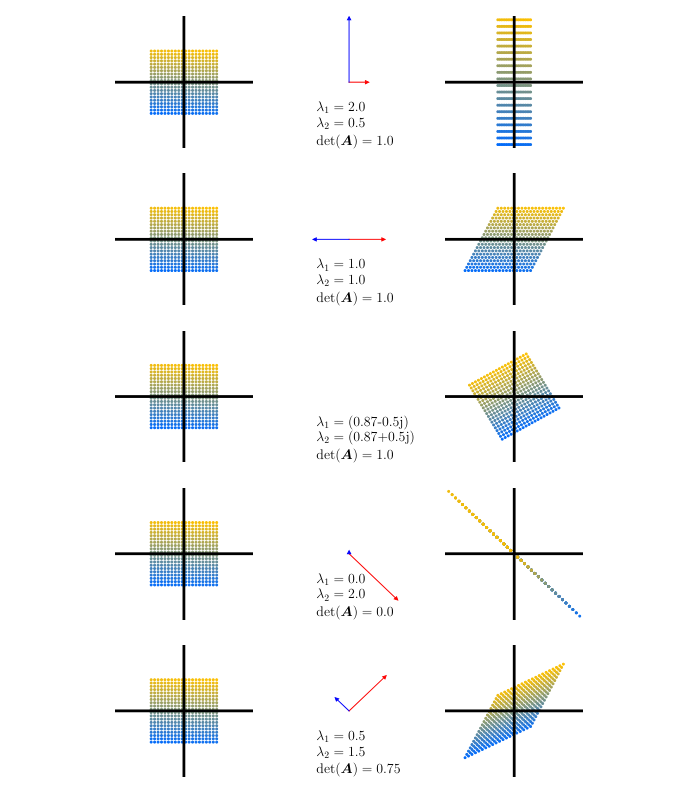
\includegraphics[width=320pt,keepaspectratio]{docs/images/Figure4.4.png}
\caption*{\refstepcounter{figcounter}\label{fig:4-4}图~\thefigcounter 行列式与特征空间。五种线性映射及其对应的变换矩阵 Aᵢ ∈ R²ˣ² 的总览，将 400 个以颜色编码的点 x ∈ R²（左列）投射到目标点 Aᵢx（右列）。中间列描绘了由其对应的特征值 λ₁ 拉伸的第一个特征向量，以及由其特征值 λ₂ 拉伸的第二个特征向量。每一行描绘了相对于标准基的五个变换矩阵 Aᵢ 之一的作用效果。}
\end{figure}


\begin{notebox}
\textbf{例 4.7（生物神经网络的特征谱）}
\end{notebox}

\begin{notebox}
分析网络数据并从中学习的方法是机器学习方法的重要组成部分。理解网络的关键是网络节点之间的连接性，特别是两个节点之间是否相互连接。在数据科学应用中，研究能够捕捉这种连接数据的矩阵通常非常有用。
\end{notebox}

\begin{notebox}
我们构建了秀丽隐杆线虫（*C. elegans*）整个神经网络的连接/邻接矩阵 $ \boldsymbol{A} \in \mathbb{R}^{277 \times 277} $。每一行/列代表该线虫大脑中 277 个神经元之一。如果神经元 $ i $ 通过突触与神经元 $ j $ 进行通信，则连接矩阵 $ \boldsymbol{A} $ 的元素值为 $ a_{ij} = 1 $，否则 $ a_{ij} = 0 $。该连接矩阵不是对称矩阵，这意味着特征值可能不是实数。因此，我们计算连接矩阵的对称化版本 $ \boldsymbol{A}_{\text{sym}} := \boldsymbol{A} + \boldsymbol{A}^\top $。这个新矩阵 $ \boldsymbol{A}_{\text{sym}} $ 如图~\ref{fig:4-5}(a) 所示，当且仅当两个神经元相连时具有非零值 $ a_{ij} $（白色像素），无论连接的方向如何。在图~\ref{fig:4-5}(b) 中，我们展示了 $ \boldsymbol{A}_{\text{sym}} $ 对应的特征谱。横轴表示按降序排列的特征值的索引。纵轴表示对应的特征值。这种特征谱的 S 形曲线是许多生物神经网络的典型特征。导致这一现象的潜在机制是目前神经科学活跃的研究领域。
\end{notebox}


\begin{figure}[H]
\centering
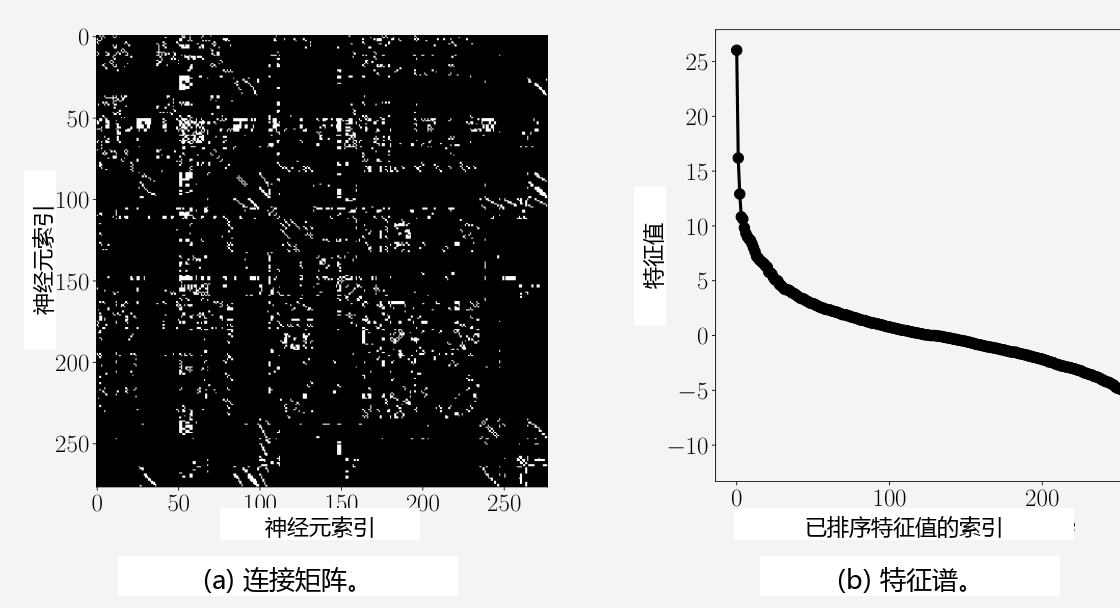
\includegraphics[width=0.92\textwidth,keepaspectratio]{docs/images/Figure4.5.png}
\caption*{\refstepcounter{figcounter}\label{fig:4-5}图~\thefigcounter 秀丽隐杆线虫（Caenorhabditis elegans）神经网络（Kaiser and Hilgetag, 2006）。(a) 对称化连接矩阵；(b) 特征谱。}
\end{figure}


\textbf{定理 4.12}。具有 $ n $ 个互不相同特征值 $ \lambda_1, \ldots, \lambda_n $ 的矩阵 $ \boldsymbol{A} \in \mathbb{R}^{n \times n} $ 的特征向量 $ \boldsymbol{x}_1, \ldots, \boldsymbol{x}_n $ 是线性无关的。

该定理表明，具有 $ n $ 个互不相同特征值的矩阵的特征向量构成了 $ \mathbb{R}^n $ 的一组基。

\textbf{定义 4.13}（亏损矩阵）。若方阵 $ \boldsymbol{A} \in \mathbb{R}^{n \times n} $ 拥有的线性无关特征向量少于 $ n $ 个，则称其为 \emph{亏损矩阵（defective matrix）} 。

非亏损矩阵 $ \boldsymbol{A} \in \mathbb{R}^{n \times n} $ 并不一定需要 $ n $ 个互不相同的特征值，但它确实要求特征向量构成 $ \mathbb{R}^n $ 的一组基。从亏损矩阵的特征空间来看，亏损矩阵的特征空间维数之和小于 $ n $。具体而言，亏损矩阵至少有一个代数重数 $ m > 1 $ 的特征值 $ \lambda_i $，其几何重数小于 $ m $。

\emph{备注} 。亏损矩阵不可能拥有 $ n $ 个互不相同的特征值，因为互不相同的特征值对应线性无关的特征向量（定理 4.12）。♦

\textbf{定理 4.14}。给定矩阵 $ \boldsymbol{A} \in \mathbb{R}^{m \times n} $，我们总是可以通过定义：

\begin{equation}
\boldsymbol{S} := \boldsymbol{A}^\top \boldsymbol{A}
\tag{4.36}\label{eq:4-36}
\end{equation}

获得一个对称半正定矩阵 $ \boldsymbol{S} \in \mathbb{R}^{n \times n} $。

\emph{备注} 。若 $ \operatorname{rk}(\boldsymbol{A}) = n $，则 $ \boldsymbol{S} := \boldsymbol{A}^\top \boldsymbol{A} $ 是对称正定的。♦

理解定理 4.14 成立的原因有助于我们认识如何利用对称化矩阵：对称性要求 $ \boldsymbol{S} = \boldsymbol{S}^\top $，代入式~\eqref{eq:4-36} 得到

\begin{equation*}
\boldsymbol{S} = \boldsymbol{A}^\top \boldsymbol{A} = \boldsymbol{A}^\top (\boldsymbol{A}^\top)^\top = (\boldsymbol{A}^\top \boldsymbol{A})^\top = \boldsymbol{S}^\top
\end{equation*}

。此外，半正定性（第 3.2.3 节）要求 $ \boldsymbol{x}^\top \boldsymbol{S} \boldsymbol{x} \ge 0 $，代入式~\eqref{eq:4-36} 得到

\begin{equation*}
\begin{adjustbox}{max width=\linewidth}
\boldsymbol{x}^\top \boldsymbol{S} \boldsymbol{x} = \boldsymbol{x}^\top \boldsymbol{A}^\top \boldsymbol{A} \boldsymbol{x} = (\boldsymbol{x}^\top \boldsymbol{A}^\top)(\boldsymbol{A} \boldsymbol{x}) = (\boldsymbol{A} \boldsymbol{x})^\top (\boldsymbol{A} \boldsymbol{x}) \ge 0
\end{adjustbox}
\end{equation*}

，因为点积计算的是平方和（其本身非负）。

\textbf{定理 4.15}（谱定理 / Spectral Theorem）。若 $ \boldsymbol{A} \in \mathbb{R}^{n \times n} $ 是对称的，则存在由 $ \boldsymbol{A} $ 的特征向量构成的对应向量空间 $ V $ 的标准正交基，且每个特征值均为实数。

谱定理的一个直接推论是：对称矩阵 $ \boldsymbol{A} $ 的特征分解存在（具有实特征值），并且我们可以找到由特征向量构成的标准正交基，使得 $ \boldsymbol{A} = \boldsymbol{P} \boldsymbol{D} \boldsymbol{P}^\top $，其中 $ \boldsymbol{D} $ 为对角矩阵，而 $ \boldsymbol{P} $ 的各列包含这些特征向量。

\begin{notebox}
\textbf{例 4.8}
\end{notebox}

\begin{notebox}
考虑矩阵：

\begin{equation}
\boldsymbol{A} = \begin{bmatrix} 3 & 2 & 2 \\ 2 & 3 & 2 \\ 2 & 2 & 3 \end{bmatrix}
\tag{4.37}\label{eq:4-37}
\end{equation}

$ \boldsymbol{A} $ 的特征多项式为：

\begin{equation}
p_{\boldsymbol{A}}(\lambda) = -(\lambda - 1)^2(\lambda - 7)
\tag{4.38}\label{eq:4-38}
\end{equation}

由此我们得到特征值 $ \lambda_1 = 1 $ 和 $ \lambda_2 = 7 $，其中 $ \lambda_1 $ 是重特征值。按照我们计算特征向量的标准步骤，得到特征空间：

\begin{equation}
\begin{adjustbox}{max width=\linewidth}
E_1 = \operatorname{span}\left[\underbrace{\begin{bmatrix} -1 \\ 1 \\ 0 \end{bmatrix}}_{=: \boldsymbol{x}_1}, \underbrace{\begin{bmatrix} -1 \\ 0 \\ 1 \end{bmatrix}}_{=: \boldsymbol{x}_2}\right], \quad E_7 = \operatorname{span}\left[\underbrace{\begin{bmatrix} 1 \\ 1 \\ 1 \end{bmatrix}}_{=: \boldsymbol{x}_3}\right]
\end{adjustbox}
\tag{4.39}\label{eq:4-39}
\end{equation}

我们看到 $ \boldsymbol{x}_3 $ 与 $ \boldsymbol{x}_1 $ 和 $ \boldsymbol{x}_2 $ 都正交。然而，由于 $ \boldsymbol{x}_1^\top \boldsymbol{x}_2 = 1 \neq 0 $，它们彼此不正交。谱定理（定理 4.15）指出存在正交基，但我们现有的这组基并不是正交的。不过，我们可以构造出一组正交基。
\end{notebox}

\begin{notebox}
为了构造这样的基，我们利用 $ \boldsymbol{x}_1, \boldsymbol{x}_2 $ 是对应于相同特征值 $ \lambda $ 的特征向量这一事实。因此，对于任意 $ \alpha, \beta \in \mathbb{R} $，都有：

\begin{equation}
\boldsymbol{A}(\alpha \boldsymbol{x}_1 + \beta \boldsymbol{x}_2) = \boldsymbol{A} \boldsymbol{x}_1 \alpha + \boldsymbol{A} \boldsymbol{x}_2 \beta = \lambda(\alpha \boldsymbol{x}_1 + \beta \boldsymbol{x}_2)
\tag{4.40}\label{eq:4-40}
\end{equation}

即 $ \boldsymbol{x}_1 $ 和 $ \boldsymbol{x}_2 $ 的任意线性组合也是 $ \boldsymbol{A} $ 对应于 $ \lambda $ 的特征向量。格拉姆-施密特算法（Gram-Schmidt algorithm，第 3.8.3 节）是一种利用此类线性组合从一组基向量中迭代构造正交/标准正交基的方法。因此，即使 $ \boldsymbol{x}_1 $ 和 $ \boldsymbol{x}_2 $ 不正交，我们也可以应用格拉姆-施密特算法，找到对应于 $ \lambda_1 = 1 $ 且彼此正交（并与 $ \boldsymbol{x}_3 $ 正交）的特征向量。在我们的示例中，我们将得到：

\begin{equation}
\boldsymbol{x}_1' = \begin{bmatrix} -1 \\ 1 \\ 0 \end{bmatrix}, \quad \boldsymbol{x}_2' = \frac{1}{2} \begin{bmatrix} -1 \\ -1 \\ 2 \end{bmatrix}
\tag{4.41}\label{eq:4-41}
\end{equation}

它们彼此正交，与 $ \boldsymbol{x}_3 $ 正交，并且是 $ \boldsymbol{A} $ 对应于 $ \lambda_1 = 1 $ 的特征向量。
\end{notebox}

在我们结束对特征值和特征向量的讨论之前，将这些矩阵特征与行列式和迹的概念联系起来是有益的。

\textbf{定理 4.16}。矩阵 $ \boldsymbol{A} \in \mathbb{R}^{n \times n} $ 的行列式是其特征值的乘积，即：

\begin{equation}
\det(\boldsymbol{A}) = \prod_{i=1}^n \lambda_i
\tag{4.42}\label{eq:4-42}
\end{equation}

其中 $ \lambda_i $ 是 $ \boldsymbol{A} $ 的特征值（计入重数）。

\textbf{定理 4.17}。矩阵 $ \boldsymbol{A} \in \mathbb{R}^{n \times n} $ 的迹是其特征值的和，即：

\begin{equation}
\operatorname{tr}(\boldsymbol{A}) = \sum_{i=1}^n \lambda_i
\tag{4.43}\label{eq:4-43}
\end{equation}

其中 $ \lambda_i $ 是 $ \boldsymbol{A} $ 的特征值（计入重数）。


\begin{figure}[H]
\centering
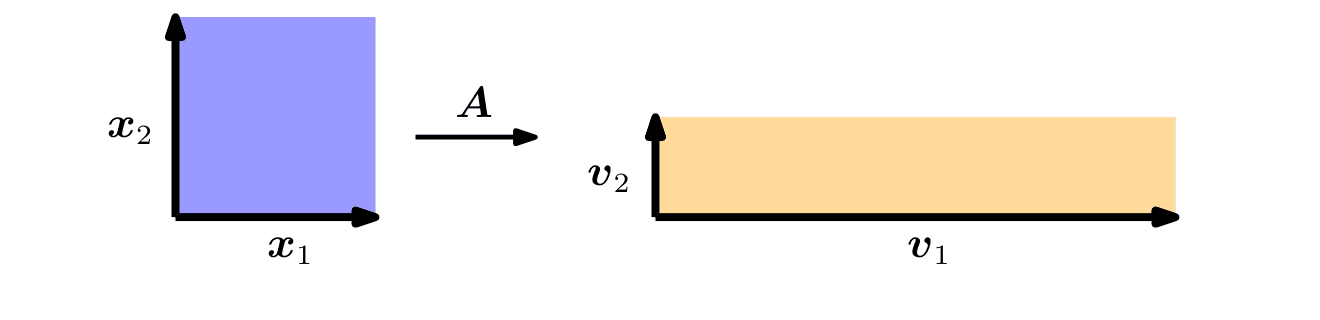
\includegraphics[width=0.92\textwidth,keepaspectratio]{docs/images/Figure4.6.png}
\caption*{\refstepcounter{figcounter}\label{fig:4-6}图~\thefigcounter 特征值的几何解释。A 的特征向量被对应的特征值拉伸。单位正方形的面积改变了 |λ₁λ₂| 倍，周长改变了 2(|λ₁| + |λ₂|) 倍。}
\end{figure}


让我们为这两个定理提供一种几何直觉。考虑一个拥有两个线性无关特征向量 $ \boldsymbol{x}_1, \boldsymbol{x}_2 $ 的矩阵 $ \boldsymbol{A} \in \mathbb{R}^{2 \times 2} $。对于本例，我们假设 $ (\boldsymbol{x}_1, \boldsymbol{x}_2) $ 是 $ \mathbb{R}^2 $ 的一组标准正交基，因此它们相互正交，且它们所张成的正方形面积为 1；参见图~\ref{fig:4-6}。由第 4.1 节可知，行列式计算了在变换 $ \boldsymbol{A} $ 作用下单位正方形面积的变化。在本例中，我们可以显式计算面积的变化：使用 $ \boldsymbol{A} $ 映射特征向量得到向量 $ \boldsymbol{v}_1 = \boldsymbol{A} \boldsymbol{x}_1 = \lambda_1 \boldsymbol{x}_1 $ 和 $ \boldsymbol{v}_2 = \boldsymbol{A} \boldsymbol{x}_2 = \lambda_2 \boldsymbol{x}_2 $，即新向量 $ \boldsymbol{v}_i $ 是特征向量 $ \boldsymbol{x}_i $ 的缩放版本，缩放比例因子就是对应的特征值 $ \lambda_i $。$ \boldsymbol{v}_1, \boldsymbol{v}_2 $ 仍然正交，并且它们张成的矩形面积为 $ |\lambda_1 \lambda_2| $。

鉴于 $ \boldsymbol{x}_1, \boldsymbol{x}_2 $（在我们的示例中）是标准正交的，我们可以直接计算出单位正方形的周长为 $ 2(1 + 1) $。使用 $ \boldsymbol{A} $ 映射特征向量后得到的矩形周长为 $ 2(|\lambda_1| + |\lambda_2|) $。因此，特征值绝对值的和告诉我们，在变换矩阵 $ \boldsymbol{A} $ 的作用下，单位正方形的周长发生了怎样的变化。

\begin{notebox}
\textbf{例 4.9（谷歌的 PageRank——作为特征向量的网页）}
\end{notebox}

\begin{notebox}
谷歌使用矩阵 $ \boldsymbol{A} $ 最大特征值对应的特征向量来确定用于搜索的网页排名。1996 年由拉里·佩奇（Larry Page）和谢尔盖·布林（Sergey Brin）在斯坦福大学开发的 \emph{PageRank} 算法的核心思想是：任何网页的重要性都可以通过链接到它的网页的重要性来近似。为此，他们将所有网站写成一个巨大的有向图，展示哪个网页链接到哪个网页。PageRank 通过统计指向网站 $ a_i $ 的网页数量来计算网站 $ a_i $ 的权重（重要性）$ x_i \ge 0 $。此外，PageRank 还考虑了链接到 $ a_i $ 的网站自身的重要性。用户的浏览行为随后由该图的状态转移矩阵 $ \boldsymbol{A} $ 建模，该矩阵告诉我们用户最终跳转到另一个网站的（点击）概率是多少。矩阵 $ \boldsymbol{A} $ 具有这样的性质：对于任意给定的网站初始排名/重要性向量 $ \boldsymbol{x} $，序列 $ \boldsymbol{x}, \boldsymbol{A}\boldsymbol{x}, \boldsymbol{A}^2\boldsymbol{x}, \ldots $ 都会收敛到一个向量 $ \boldsymbol{x}^* $。这个向量被称为 PageRank，且满足 $ \boldsymbol{A} \boldsymbol{x}^* = \boldsymbol{x}^* $，即它是 $ \boldsymbol{A} $ 的特征向量（对应特征值为 1）。将 $ \boldsymbol{x}^* $ 归一化使得 $ \|\boldsymbol{x}^*\| = 1 $ 后，我们可以将其各分量解释为概率。关于 PageRank 的更多细节和不同视角，可参见原始技术报告（Page et al., 1999）。
\end{notebox}

\section*{4.3 乔莱斯基分解}
\addcontentsline{toc}{section}{4.3 乔莱斯基分解}
\label{sec:4.3}

在机器学习中经常遇到的特殊类型矩阵有许多因式分解的方法。在正实数中，开平方运算可以将一个数分解为相同分量的乘积，例如 $ 9 = 3 \cdot 3 $。对于矩阵，我们需要格外谨慎，以确保对正量进行类似开平方的运算。对于对称正定矩阵（参见第 3.2.3 节），我们可以从多种等价于开平方的运算中进行选择。 \emph{乔莱斯基分解（Cholesky decomposition）} / \emph{乔莱斯基因子分解（Cholesky factorization）} 为对称正定矩阵提供了一种在实践中非常实用的等价于开平方的运算。

\textbf{定理 4.18}（乔莱斯基分解 / Cholesky Decomposition）。对称正定矩阵 $ \boldsymbol{A} $ 可以分解为乘积 $ \boldsymbol{A} = \boldsymbol{L} \boldsymbol{L}^\top $，其中 $ \boldsymbol{L} $ 是具有正对角线元素的下三角矩阵：

\begin{equation}
\begin{adjustbox}{max width=\linewidth}
\begin{bmatrix} a_{11} & \cdots & a_{1n} \\ \vdots & \ddots & \vdots \\ a_{n1} & \cdots & a_{nn} \end{bmatrix} = \begin{bmatrix} l_{11} & \cdots & 0 \\ \vdots & \ddots & \vdots \\ l_{n1} & \cdots & l_{nn} \end{bmatrix} \begin{bmatrix} l_{11} & \cdots & l_{n1} \\ \vdots & \ddots & \vdots \\ 0 & \cdots & l_{nn} \end{bmatrix}
\end{adjustbox}
\tag{4.44}\label{eq:4-44}
\end{equation}

$ \boldsymbol{L} $ 称为 $ \boldsymbol{A} $ 的 \emph{乔莱斯基因子（Cholesky factor）} ，且 $ \boldsymbol{L} $ 是唯一的。

\begin{notebox}
\textbf{例 4.10（乔莱斯基分解）}
\end{notebox}

\begin{notebox}
考虑一个对称正定矩阵 $ \boldsymbol{A} \in \mathbb{R}^{3 \times 3} $。我们希望求出其乔莱斯基分解 $ \boldsymbol{A} = \boldsymbol{L} \boldsymbol{L}^\top $，即：

\begin{equation}
\begin{adjustbox}{max width=\linewidth}
\boldsymbol{A} = \begin{bmatrix} a_{11} & a_{21} & a_{31} \\ a_{21} & a_{22} & a_{32} \\ a_{31} & a_{32} & a_{33} \end{bmatrix} = \boldsymbol{L} \boldsymbol{L}^\top = \begin{bmatrix} l_{11} & 0 & 0 \\ l_{21} & l_{22} & 0 \\ l_{31} & l_{32} & l_{33} \end{bmatrix} \begin{bmatrix} l_{11} & l_{21} & l_{31} \\ 0 & l_{22} & l_{32} \\ 0 & 0 & l_{33} \end{bmatrix}
\end{adjustbox}
\tag{4.45}\label{eq:4-45}
\end{equation}

将右侧展开相乘得到：

\begin{equation}
\begin{adjustbox}{max width=\linewidth}
\boldsymbol{A} = \begin{bmatrix} l_{11}^2 & l_{21}l_{11} & l_{31}l_{11} \\ l_{21}l_{11} & l_{21}^2 + l_{22}^2 & l_{31}l_{21} + l_{32}l_{22} \\ l_{31}l_{11} & l_{31}l_{21} + l_{32}l_{22} & l_{31}^2 + l_{32}^2 + l_{33}^2 \end{bmatrix}
\end{adjustbox}
\tag{4.46}\label{eq:4-46}
\end{equation}

比较式~\eqref{eq:4-45} 的左侧与式~\eqref{eq:4-46} 的右侧，可以看出对角线元素 $ l_{ii} $ 具有简单的规律：

\begin{equation}
l_{11} = \sqrt{a_{11}}, \quad l_{22} = \sqrt{a_{22} - l_{21}^2}, \quad l_{33} = \sqrt{a_{33} - (l_{31}^2 + l_{32}^2)}
\tag{4.47}\label{eq:4-47}
\end{equation}

类似地，对于对角线下方的元素（$ l_{ij} $，其中 $ i > j $），也存在重复的规律：

\begin{equation}
l_{21} = \frac{1}{l_{11}} a_{21}, \quad l_{31} = \frac{1}{l_{11}} a_{31}, \quad l_{32} = \frac{1}{l_{22}} (a_{32} - l_{31}l_{21})
\tag{4.48}\label{eq:4-48}
\end{equation}

这样，我们就为任意对称正定 $ 3 \times 3 $ 矩阵构造出了乔莱斯基分解。关键的认识在于，给定矩阵 $ \boldsymbol{A} $ 的元素值 $ a_{ij} $ 以及先前计算出的 $ l_{ij} $ 值，我们可以逆向回代计算出矩阵 $ \boldsymbol{L} $ 的分量 $ l_{ij} $ 应该是多少。
\end{notebox}

乔莱斯基分解是机器学习底层数值计算的重要工具。在这里，对称正定矩阵需要频繁进行运算操作，例如多元高斯变量的协方差矩阵（参见第 6.5 节）就是对称正定的。该协方差矩阵的乔莱斯基分解使我们能够从高斯分布中生成样本。它还允许我们对随机变量进行线性变换，这在计算深度随机模型（如变分自编码器（variational auto-encoder, Jimenez Rezende et al., 2014; Kingma and Welling, 2014））中的梯度时被大量采用。乔莱斯基分解还使我们能够非常高效地计算行列式。给定乔莱斯基分解 $ \boldsymbol{A} = \boldsymbol{L} \boldsymbol{L}^\top $，我们知道 $ \det(\boldsymbol{A}) = \det(\boldsymbol{L}) \det(\boldsymbol{L}^\top) = \det(\boldsymbol{L})^2 $。由于 $ \boldsymbol{L} $ 是三角矩阵，其行列式就是对角线元素的乘积，因此 $ \det(\boldsymbol{A}) = \prod_i l_{ii}^2 $。因此，许多数值计算软件包都使用乔莱斯基分解来提高计算效率。

\section*{4.4 特征分解与对角化}
\addcontentsline{toc}{section}{4.4 特征分解与对角化}
\label{sec:4.4}

\emph{对角矩阵（diagonal matrix）} 是指所有非主对角线元素均为零的矩阵，即它们具有如下形式：

\begin{equation}
\boldsymbol{D} = \begin{bmatrix} c_1 & \cdots & 0 \\ \vdots & \ddots & \vdots \\ 0 & \cdots & c_n \end{bmatrix}
\tag{4.49}\label{eq:4-49}
\end{equation}

对角矩阵允许我们快速计算行列式、幂以及逆矩阵。其行列式是对角线上各元素的乘积，矩阵的幂 $ \boldsymbol{D}^k $ 是通过将每个对角线元素取 $ k $ 次幂得到的，而当对角线元素均非零时，其逆矩阵 $ \boldsymbol{D}^{-1} $ 的对角线元素即为原对角线元素的倒数。在本节中，我们将讨论如何将矩阵转换为对角形式。这是我们在第 2.7.2 节中讨论的基变换以及第 4.2 节中讨论的特征值的一个重要应用。

回顾一下，如果存在可逆矩阵 $ \boldsymbol{P} $ 使得 $ \boldsymbol{D} = \boldsymbol{P}^{-1} \boldsymbol{A} \boldsymbol{P} $，则称两个矩阵 $ \boldsymbol{A}, \boldsymbol{D} $ 是相似的（定义 2.22）。更具体地说，我们将研究与对角矩阵 $ \boldsymbol{D} $ 相似的矩阵 $ \boldsymbol{A} $，其中 $ \boldsymbol{D} $ 的对角线上包含 $ \boldsymbol{A} $ 的特征值。

\textbf{定义 4.19}（可对角化 / Diagonalizable）。如果方阵 $ \boldsymbol{A} \in \mathbb{R}^{n \times n} $ 与某个对角矩阵相似，即存在可逆矩阵 $ \boldsymbol{P} \in \mathbb{R}^{n \times n} $ 使得 $ \boldsymbol{D} = \boldsymbol{P}^{-1} \boldsymbol{A} \boldsymbol{P} $，则称 $ \boldsymbol{A} $ 是 \emph{可对角化的（diagonalizable）} 。

在下文中，我们将看到对矩阵 $ \boldsymbol{A} \in \mathbb{R}^{n \times n} $ 进行对角化是在另一组基下表示同一线性映射的一种方式（参见第 2.6.1 节），并且事实表明这组基由 $ \boldsymbol{A} $ 的特征向量组成。

设 $ \boldsymbol{A} \in \mathbb{R}^{n \times n} $，设 $ \lambda_1, \ldots, \lambda_n $ 是一组标量，并设 $ \boldsymbol{p}_1, \ldots, \boldsymbol{p}_n $ 是 $ \mathbb{R}^n $ 中的一组向量。我们定义 $ \boldsymbol{P} := [\boldsymbol{p}_1, \ldots, \boldsymbol{p}_n] $，并设 $ \boldsymbol{D} \in \mathbb{R}^{n \times n} $ 是对角线元素为 $ \lambda_1, \ldots, \lambda_n $ 的对角矩阵。那么我们可以证明：

\begin{equation}
\boldsymbol{A} \boldsymbol{P} = \boldsymbol{P} \boldsymbol{D}
\tag{4.50}\label{eq:4-50}
\end{equation}

当且仅当 $ \lambda_1, \ldots, \lambda_n $ 是 $ \boldsymbol{A} $ 的特征值，且 $ \boldsymbol{p}_1, \ldots, \boldsymbol{p}_n $ 是 $ \boldsymbol{A} $ 对应的特征向量。

我们可以看到该命题成立，因为：

\begin{equation}
\boldsymbol{A} \boldsymbol{P} = \boldsymbol{A} [\boldsymbol{p}_1, \ldots, \boldsymbol{p}_n] = [\boldsymbol{A} \boldsymbol{p}_1, \ldots, \boldsymbol{A} \boldsymbol{p}_n]
\tag{4.51}\label{eq:4-51}
\end{equation}

\begin{equation}
\begin{adjustbox}{max width=\linewidth}
\boldsymbol{P} \boldsymbol{D} = [\boldsymbol{p}_1, \ldots, \boldsymbol{p}_n] \begin{bmatrix} \lambda_1 & & 0 \\ & \ddots & \\ 0 & & \lambda_n \end{bmatrix} = [\lambda_1 \boldsymbol{p}_1, \ldots, \lambda_n \boldsymbol{p}_n]
\end{adjustbox}
\tag{4.52}\label{eq:4-52}
\end{equation}

因此，式~\eqref{eq:4-50} 意味着：

\begin{equation}
\boldsymbol{A} \boldsymbol{p}_1 = \lambda_1 \boldsymbol{p}_1
\tag{4.53}\label{eq:4-53}
\end{equation}

\begin{equation*}
\vdots
\end{equation*}

\begin{equation}
\boldsymbol{A} \boldsymbol{p}_n = \lambda_n \boldsymbol{p}_n
\tag{4.54}\label{eq:4-54}
\end{equation}

所以，$ \boldsymbol{P} $ 的各列必须是 $ \boldsymbol{A} $ 的特征向量。

我们对对角化的定义要求 $ \boldsymbol{P} \in \mathbb{R}^{n \times n} $ 是可逆的，即 $ \boldsymbol{P} $ 具有满秩（定理 4.3）。这要求我们拥有 $ n $ 个线性无关的特征向量 $ \boldsymbol{p}_1, \ldots, \boldsymbol{p}_n $，即 $ \boldsymbol{p}_i $ 构成 $ \mathbb{R}^n $ 的一组基。

\textbf{定理 4.20}（特征分解 / Eigendecomposition）。方阵 $ \boldsymbol{A} \in \mathbb{R}^{n \times n} $ 可以分解为

\begin{equation}
\boldsymbol{A} = \boldsymbol{P} \boldsymbol{D} \boldsymbol{P}^{-1}
\tag{4.55}\label{eq:4-55}
\end{equation}

其中 $ \boldsymbol{P} \in \mathbb{R}^{n \times n} $，且 $ \boldsymbol{D} $ 是对角线元素为 $ \boldsymbol{A} $ 的特征值的对角矩阵，当且仅当 $ \boldsymbol{A} $ 的特征向量构成 $ \mathbb{R}^n $ 的一组基。


\begin{figure}[H]
\centering
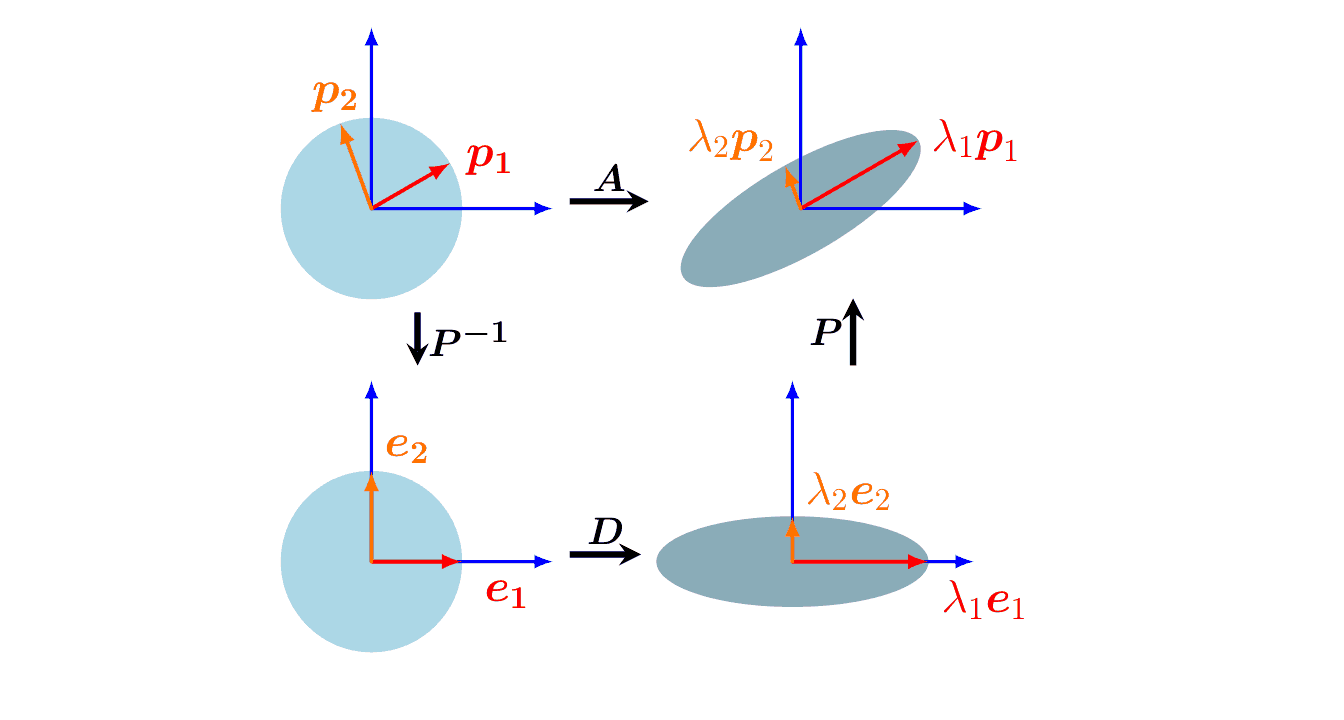
\includegraphics[width=0.92\textwidth,keepaspectratio]{docs/images/Figure4.7.png}
\caption*{\refstepcounter{figcounter}\label{fig:4-7}图~\thefigcounter 将特征分解理解为一系列连续变换的几何直观。左上到左下：P⁻¹ 执行基变换（此处在 R² 中绘制，表示为类似旋转的操作），将特征向量映射到标准基。左下到右下：D 沿着重新映射的正交特征向量进行缩放，此处由圆拉伸为椭圆来表示。右下到右上：P 撤销基变换（表示为反向旋转）并恢复原始坐标系。}
\end{figure}


定理 4.20 表明只有非亏损矩阵才可以对角化，并且 $ \boldsymbol{P} $ 的各列是 $ \boldsymbol{A} $ 的 $ n $ 个特征向量。对于对称矩阵，我们可以在特征值分解方面获得更强的结论。

\textbf{定理 4.21}。对称矩阵 $ \boldsymbol{S} \in \mathbb{R}^{n \times n} $ 总是可以对角化的。

定理 4.21 直接由谱定理（定理 4.15）得出。此外，谱定理指出我们可以找到由 $ \mathbb{R}^n $ 的特征向量构成的标准正交基（ONB）。这使得 $ \boldsymbol{P} $ 成为正交矩阵，从而 $ \boldsymbol{D} = \boldsymbol{P}^\top \boldsymbol{A} \boldsymbol{P} $。

\emph{备注} 。矩阵的若尔当标准形（Jordan normal form）提供了一种适用于亏损矩阵的分解方法（Lang, 1987），但这超出了本书的讨论范围。♦

\section*{特征分解的几何直观}
\addcontentsline{toc}{subsection}{特征分解的几何直观}

我们可以将矩阵的特征分解解释如下（亦见图~\ref{fig:4-7}）：设 $ \boldsymbol{A} $ 为关于标准基的线性映射的变换矩阵。$ \boldsymbol{P}^{-1} $ 执行从标准基到特征基的基变换。这把特征向量 $ \boldsymbol{p}_i $（图~\ref{fig:4-7} 中的红色和橙色箭头）映射到标准基向量 $ \boldsymbol{e}_i $ 上。然后，对角矩阵 $ \boldsymbol{D} $ 沿着这些坐标轴按特征值 $ \lambda_i $ 对向量进行缩放。最后，$ \boldsymbol{P} $ 将这些缩放后的向量变换回标准/规范坐标系，得到 $ \lambda_i \boldsymbol{p}_i $。

\begin{notebox}
\textbf{例 4.11（特征分解）}
\end{notebox}

\begin{notebox}
我们来计算矩阵

\begin{equation*}
\boldsymbol{A} = \begin{bmatrix} 2 & 1 \\ 1 & 2 \end{bmatrix}
\end{equation*}

的特征分解。
\end{notebox}

\begin{notebox}
\textbf{步骤 1：计算特征值和特征向量。} $ \boldsymbol{A} $ 的特征多项式为：

\begin{equation}
\det(\boldsymbol{A} - \lambda \boldsymbol{I}) = \det\begin{bmatrix} 2 - \lambda & 1 \\ 1 & 2 - \lambda \end{bmatrix}
\tag{4.56a}\label{eq:4-56a}
\end{equation}

\begin{equation}
= (2 - \lambda)^2 - 1 = \lambda^2 - 4\lambda + 3 = (\lambda - 3)(\lambda - 1)
\tag{4.56b}\label{eq:4-56b}
\end{equation}

因此，$ \boldsymbol{A} $ 的特征值为 $ \lambda_1 = 1 $ 和 $ \lambda_2 = 3 $（特征多项式的根），对应的（归一化）特征向量通过下式求得：

\begin{equation}
\begin{bmatrix} 2 & 1 \\ 1 & 2 \end{bmatrix} \boldsymbol{p}_1 = 1 \boldsymbol{p}_1, \quad \begin{bmatrix} 2 & 1 \\ 1 & 2 \end{bmatrix} \boldsymbol{p}_2 = 3 \boldsymbol{p}_2
\tag{4.57}\label{eq:4-57}
\end{equation}

由此解得：

\begin{equation}
\boldsymbol{p}_1 = \frac{1}{\sqrt{2}} \begin{bmatrix} 1 \\ -1 \end{bmatrix}, \quad \boldsymbol{p}_2 = \frac{1}{\sqrt{2}} \begin{bmatrix} 1 \\ 1 \end{bmatrix}
\tag{4.58}\label{eq:4-58}
\end{equation}
\end{notebox}

\begin{notebox}
\textbf{步骤 2：检验存在性。} 特征向量 $ \boldsymbol{p}_1, \boldsymbol{p}_2 $ 构成 $ \mathbb{R}^2 $ 的一组基。因此，$ \boldsymbol{A} $ 可以对角化。
\end{notebox}

\begin{notebox}
\textbf{步骤 3：构造对角化 $ \boldsymbol{A} $ 的矩阵 $ \boldsymbol{P} $。} 我们将 $ \boldsymbol{A} $ 的特征向量组合在 $ \boldsymbol{P} $ 中，使得：

\begin{equation}
\boldsymbol{P} = [\boldsymbol{p}_1, \boldsymbol{p}_2] = \frac{1}{\sqrt{2}} \begin{bmatrix} 1 & 1 \\ -1 & 1 \end{bmatrix}
\tag{4.59}\label{eq:4-59}
\end{equation}

接着我们得到：

\begin{equation}
\boldsymbol{P}^{-1} \boldsymbol{A} \boldsymbol{P} = \begin{bmatrix} 1 & 0 \\ 0 & 3 \end{bmatrix} = \boldsymbol{D}
\tag{4.60}\label{eq:4-60}
\end{equation}

等价地，我们得到（利用在本例中特征向量 $ \boldsymbol{p}_1 $ 和 $ \boldsymbol{p}_2 $ 构成一组标准正交基，从而 $ \boldsymbol{P}^{-1} = \boldsymbol{P}^\top $）：

\begin{equation}
\begin{adjustbox}{max width=\linewidth}
\underbrace{\begin{bmatrix} 2 & 1 \\ 1 & 2 \end{bmatrix}}_{\boldsymbol{A}} = \underbrace{\frac{1}{\sqrt{2}} \begin{bmatrix} 1 & 1 \\ -1 & 1 \end{bmatrix}}_{\boldsymbol{P}} \underbrace{\begin{bmatrix} 1 & 0 \\ 0 & 3 \end{bmatrix}}_{\boldsymbol{D}} \underbrace{\frac{1}{\sqrt{2}} \begin{bmatrix} 1 & -1 \\ 1 & 1 \end{bmatrix}}_{\boldsymbol{P}^\top}
\end{adjustbox}
\tag{4.61}\label{eq:4-61}
\end{equation}
\end{notebox}

对角矩阵 $ \boldsymbol{D} $ 可以非常高效地进行求幂运算。因此，我们可以通过特征值分解（如果存在）来计算矩阵 $ \boldsymbol{A} \in \mathbb{R}^{n \times n} $ 的幂，使得：

\begin{equation}
\boldsymbol{A}^k = (\boldsymbol{P} \boldsymbol{D} \boldsymbol{P}^{-1})^k = \boldsymbol{P} \boldsymbol{D}^k \boldsymbol{P}^{-1}
\tag{4.62}\label{eq:4-62}
\end{equation}

计算 $ \boldsymbol{D}^k $ 是高效的，因为我们只需对每个对角线元素分别进行该操作。

假设特征分解 $ \boldsymbol{A} = \boldsymbol{P} \boldsymbol{D} \boldsymbol{P}^{-1} $ 存在。那么：

\begin{equation}
\det(\boldsymbol{A}) = \det(\boldsymbol{P} \boldsymbol{D} \boldsymbol{P}^{-1}) = \det(\boldsymbol{P}) \det(\boldsymbol{D}) \det(\boldsymbol{P}^{-1})
\tag{4.63a}\label{eq:4-63a}
\end{equation}

\begin{equation}
= \det(\boldsymbol{D}) = \prod_{i=1}^n d_{ii}
\tag{4.63b}\label{eq:4-63b}
\end{equation}

这使得我们可以高效地计算 $ \boldsymbol{A} $ 的行列式。

特征值分解要求矩阵是方阵。若能对一般矩阵执行分解将会非常有用。在下一节中，我们将介绍一种更一般的矩阵分解技术：奇异值分解。

\section*{4.5 奇异值分解}
\addcontentsline{toc}{section}{4.5 奇异值分解}
\label{sec:4.5}

矩阵的 \emph{奇异值分解（singular value decomposition，简称 SVD）} 是线性代数中的核心矩阵分解方法之一。它被称为“线性代数的基本定理”（Strang, 1993），因为它可以应用于所有矩阵，而不仅仅是方阵，并且它总是存在的。此外，正如我们将在下文中探讨的那样，表示线性映射 $ \Phi : V \to W $ 的矩阵 $ \boldsymbol{A} $ 的 SVD，量化了这两个向量空间底层几何之间的变化。我们推荐阅读 Kalman (1996) 以及 Roy 和 Banerjee (2014) 的著作，以更深入地了解 SVD 的数学理论。

\textbf{定理 4.22}（奇异值分解定理 / SVD Theorem）。设 $ \boldsymbol{A} \in \mathbb{R}^{m \times n} $ 是秩为 $ r \in [0, \min(m, n)] $ 的长方矩阵。$ \boldsymbol{A} $ 的 SVD 是具有如下形式的分解：

\begin{equation}
\underbrace{\boldsymbol{A}}_{m \times n} = \underbrace{\boldsymbol{U}}_{m \times m} \underbrace{\boldsymbol{\Sigma}}_{m \times n} \underbrace{\boldsymbol{V}^\top}_{n \times n}
\tag{4.64}\label{eq:4-64}
\end{equation}

其中 $ \boldsymbol{U} \in \mathbb{R}^{m \times m} $ 是列向量为 $ \boldsymbol{u}_i $（$ i = 1, \ldots, m $）的正交矩阵，$ \boldsymbol{V} \in \mathbb{R}^{n \times n} $ 是列向量为 $ \boldsymbol{v}_j $（$ j = 1, \ldots, n $）的正交矩阵。此外，$ \boldsymbol{\Sigma} $ 是一个 $ m \times n $ 矩阵，满足 $ \Sigma_{ii} = \sigma_i \ge 0 $，且当 $ i \neq j $ 时 $ \Sigma_{ij} = 0 $。

$ \boldsymbol{\Sigma} $ 的对角线元素 $ \sigma_i $（$ i = 1, \ldots, r $）称为 \emph{奇异值（singular values）} ，$ \boldsymbol{u}_i $ 称为 \emph{左奇异向量（left-singular vectors）} ，$ \boldsymbol{v}_j $ 称为 \emph{右奇异向量（right-singular vectors）} 。按照惯例，奇异值是有序排列的，即 $ \sigma_1 \ge \sigma_2 \ge \cdots \ge \sigma_r \ge 0 $。

\emph{奇异值矩阵（singular value matrix）} $ \boldsymbol{\Sigma} $ 是唯一的，但需要注意其结构。请注意 $ \boldsymbol{\Sigma} \in \mathbb{R}^{m \times n} $ 是长方形的。特别地，$ \boldsymbol{\Sigma} $ 与 $ \boldsymbol{A} $ 具有相同的尺寸。这意味着 $ \boldsymbol{\Sigma} $ 包含一个存放奇异值的对角子矩阵，并且需要额外的零填充。具体而言，如果 $ m > n $，则矩阵 $ \boldsymbol{\Sigma} $ 在前 $ n $ 行具有对角结构，从第 $ n + 1 $ 行到第 $ m $ 行由行向量 $ \boldsymbol{0}^\top $ 填充，即：

\begin{equation}
\begin{adjustbox}{max width=\linewidth}
\boldsymbol{\Sigma} = \begin{bmatrix} \sigma_1 & 0 & \cdots & 0 \\ 0 & \sigma_2 & \cdots & 0 \\ \vdots & \vdots & \ddots & \vdots \\ 0 & 0 & \cdots & \sigma_n \\ 0 & 0 & \cdots & 0 \\ \vdots & \vdots & \ddots & \vdots \\ 0 & 0 & \cdots & 0 \end{bmatrix}
\end{adjustbox}
\tag{4.65}\label{eq:4-65}
\end{equation}

如果 $ m < n $，矩阵 $ \boldsymbol{\Sigma} $ 在前 $ m $ 列具有对角结构，从第 $ m + 1 $ 列到第 $ n $ 列由全 0 列向量构成：

\begin{equation}
\begin{adjustbox}{max width=\linewidth}
\boldsymbol{\Sigma} = \begin{bmatrix} \sigma_1 & 0 & \cdots & 0 & 0 & \cdots & 0 \\ 0 & \sigma_2 & \cdots & 0 & 0 & \cdots & 0 \\ \vdots & \vdots & \ddots & \vdots & \vdots & \ddots & \vdots \\ 0 & 0 & \cdots & \sigma_m & 0 & \cdots & 0 \end{bmatrix}
\end{adjustbox}
\tag{4.66}\label{eq:4-66}
\end{equation}

\emph{备注} 。SVD 对任意矩阵 $ \boldsymbol{A} \in \mathbb{R}^{m \times n} $ 都存在。♦


\begin{figure}[H]
\centering
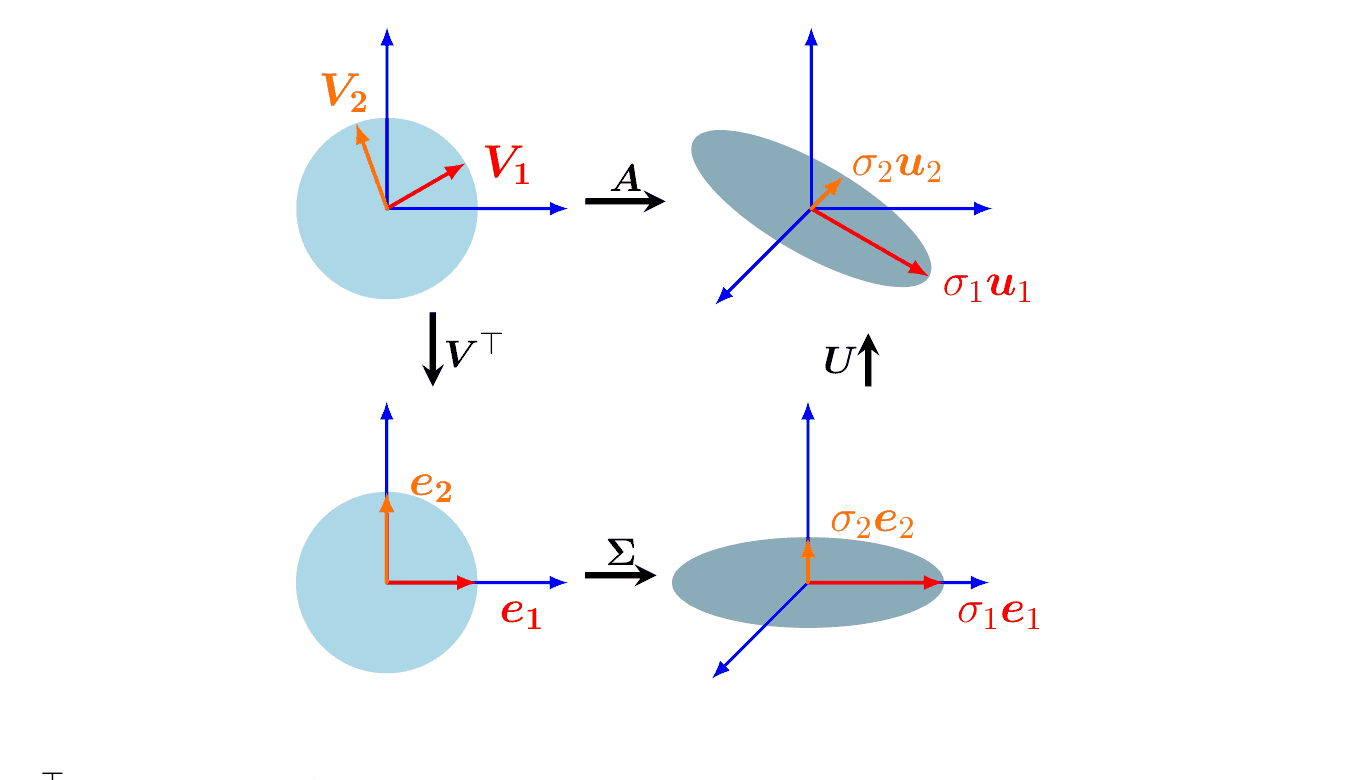
\includegraphics[width=0.92\textwidth,keepaspectratio]{docs/images/Figure4.8.png}
\caption*{\refstepcounter{figcounter}\label{fig:4-8}图~\thefigcounter 将矩阵 A ∈ R³ˣ² 的 SVD 理解为一系列连续变换的几何直观。左上到左下：Vᵀ 在 R² 中执行基变换。左下到右下：Σ 进行缩放并从 R² 映射到 R³。右下方的椭圆位于 R³ 中，第三个维度正交于该椭圆盘的表面。右下到右上：U 在 R³ 内部执行基变换。}
\end{figure}


\section*{4.5.1 SVD 的几何直观}
\addcontentsline{toc}{subsection}{4.5.1 SVD 的几何直观}

SVD 为描述变换矩阵 $ \boldsymbol{A} $ 提供了直观的几何解释。在下文中，我们将把 SVD 讨论为在基上执行的一系列连续线性变换。在例 4.12 中，我们将把 SVD 的变换矩阵应用于 $ \mathbb{R}^2 $ 中的一组向量，这使我们能够更清晰地可视化每次变换的效果。

矩阵的 SVD 可以解释为将对应的线性映射（回顾第 2.7.1 节）$ \Phi : \mathbb{R}^n \to \mathbb{R}^m $ 分解为三个运算；参见图~\ref{fig:4-8}。表面上看，SVD 的几何直观遵循与特征分解直观相似的结构（参见图~\ref{fig:4-7}）：大体而言，SVD 首先通过 $ \boldsymbol{V}^\top $ 执行基变换，然后通过奇异值矩阵 $ \boldsymbol{\Sigma} $ 进行缩放以及维度的增加（或减少）。最后，它通过 $ \boldsymbol{U} $ 执行第二次基变换。SVD 包含许多重要的细节和注意事项，这就是为什么我们将更详细地回顾这一几何直观。（温习第 2.7.2 节的基变换、定义 3.8 的正交矩阵以及第 3.5 节的标准正交基将很有帮助。）

假设给定线性映射 $ \Phi : \mathbb{R}^n \to \mathbb{R}^m $ 分别关于 $ \mathbb{R}^n $ 和 $ \mathbb{R}^m $ 的标准基 $ \mathcal{B} $ 和 $ \mathcal{C} $ 的变换矩阵。此外，假设 $ \mathbb{R}^n $ 的另一组基为 $ \tilde{\mathcal{B}} $，$ \mathbb{R}^m $ 的另一组基为 $ \tilde{\mathcal{C}} $。那么：

\begin{enumerate}
\item 矩阵 $ \boldsymbol{V} $ 在定义域 $ \mathbb{R}^n $ 中执行从 $ \tilde{\mathcal{B}} $（由图~\ref{fig:4-8} 左上方的红色和橙色向量 $ \boldsymbol{v}_1 $ 和 $ \boldsymbol{v}_2 $ 表示）到标准基 $ \mathcal{B} $ 的基变换。$ \boldsymbol{V}^\top = \boldsymbol{V}^{-1} $ 执行从 $ \mathcal{B} $ 到 $ \tilde{\mathcal{B}} $ 的基变换。在图~\ref{fig:4-8} 的左下方，红色和橙色向量现在与规范基对齐。
\item 将坐标系变换为 $ \tilde{\mathcal{B}} $ 后，$ \boldsymbol{\Sigma} $ 按奇异值 $ \sigma_i $ 对新坐标进行缩放（并增加或删除维度），即 $ \boldsymbol{\Sigma} $ 是 $ \Phi $ 关于 $ \tilde{\mathcal{B}} $ 和 $ \tilde{\mathcal{C}} $ 的变换矩阵，在图~\ref{fig:4-8} 的右下方表现为红色和橙色向量被拉伸并位于 $ \boldsymbol{e}_1\text{-}\boldsymbol{e}_2 $ 平面上，该平面现在嵌入到了第三个维度中。
\item $ \boldsymbol{U} $ 在到达域 $ \mathbb{R}^m $ 中执行从 $ \tilde{\mathcal{C}} $ 到 $ \mathbb{R}^m $ 规范基的基变换，表现为红色和橙色向量旋转脱离 $ \boldsymbol{e}_1\text{-}\boldsymbol{e}_2 $ 平面。这显示在图~\ref{fig:4-8} 的右上角。
\end{enumerate}

SVD 同时表达了定义域和到达域中的基变换。这与特征分解形成鲜明对比：特征分解在同一个向量空间内进行，应用相同的基变换然后再将其撤销。SVD 的独特之处在于这两个不同的基通过奇异值矩阵 $ \boldsymbol{\Sigma} $ 同时联系在一起。

\begin{notebox}
\textbf{例 4.12（向量与 SVD）}
\end{notebox}

\begin{notebox}
考虑将以原点为中心、尺寸为 $ 2 \times 2 $ 的盒子中的 $ \mathbb{R}^2 $ 向量构成的正方形网格 $ \mathcal{X} $ 进行映射。使用标准基，我们通过下式映射这些向量：

\begin{equation}
\boldsymbol{A} = \begin{bmatrix} 1 & -0.8 \\ 0 & 1 \\ 1 & 0 \end{bmatrix} = \boldsymbol{U} \boldsymbol{\Sigma} \boldsymbol{V}^\top
\tag{4.67a}\label{eq:4-67a}
\end{equation}

\begin{equation}
= \begin{bmatrix} -0.79 & 0 & -0.62 \\ 0.38 & -0.78 & -0.49 \\ -0.48 & -0.62 & 0.62 \end{bmatrix} \begin{bmatrix} 1.62 & 0 \\ 0 & 1.0 \\ 0 & 0 \end{bmatrix} \begin{bmatrix} -0.78 & 0.62 \\ -0.62 & -0.78 \end{bmatrix}
\tag{4.67b}\label{eq:4-67b}
\end{equation}

我们从排列在网格中的一组向量 $ \mathcal{X} $（彩色点；参见图~\ref{fig:4-9} 的左上图）开始。接着我们应用 $ \boldsymbol{V}^\top \in \mathbb{R}^{2 \times 2} $，它对 $ \mathcal{X} $ 进行旋转。旋转后的向量显示在图~\ref{fig:4-9} 的左下图中。我们现在使用奇异值矩阵 $ \boldsymbol{\Sigma} $ 将这些向量映射到达域 $ \mathbb{R}^3 $（参见图~\ref{fig:4-9} 的右下图）。请注意，所有向量都位于 $ x_1\text{-}x_2 $ 平面上，第三个坐标始终为 0。在 $ x_1\text{-}x_2 $ 平面内的向量已经被奇异值进行了拉伸。
\end{notebox}

\begin{notebox}
向量 $ \mathcal{X} $ 经由 $ \boldsymbol{A} $ 直接映射到达域 $ \mathbb{R}^3 $，等价于通过 $ \boldsymbol{U} \boldsymbol{\Sigma} \boldsymbol{V}^\top $ 对 $ \mathcal{X} $ 进行变换，其中 $ \boldsymbol{U} $ 在到达域 $ \mathbb{R}^3 $ 内执行旋转，使得映射后的向量不再局限于 $ x_1\text{-}x_2 $ 平面；但如图~\ref{fig:4-9} 右上图所示，它们仍然位于同一个平面上。
\end{notebox}


\begin{figure}[H]
\centering
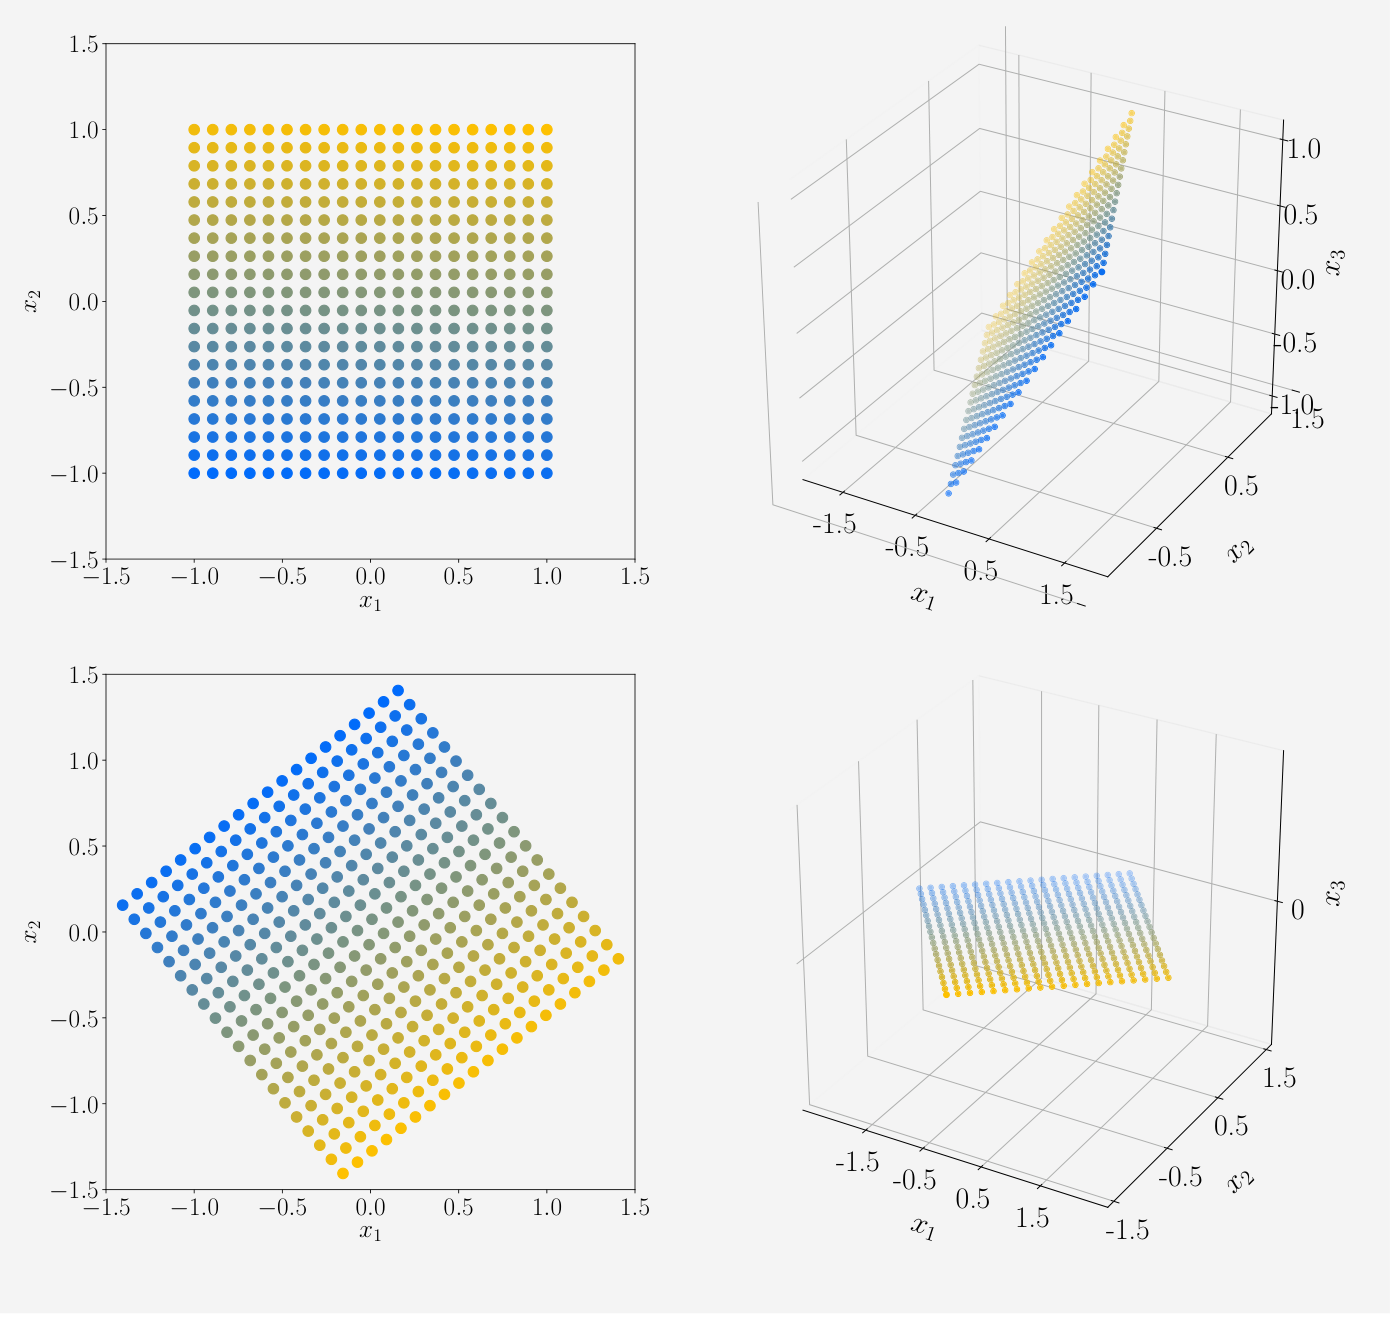
\includegraphics[width=320pt,keepaspectratio]{docs/images/Figure4.9.png}
\caption*{\refstepcounter{figcounter}\label{fig:4-9}图~\thefigcounter SVD 与向量的映射（用圆点表示）。各子图遵循与图~\ref{fig:4-8} 相同的逆时针结构。}
\end{figure}


\section*{4.5.2 SVD 的构造}
\addcontentsline{toc}{subsection}{4.5.2 SVD 的构造}

接下来我们将讨论 SVD 为什么存在，并详细说明如何计算它。一般矩阵的 SVD 与方阵的特征分解有一些相似之处。

\emph{备注} 。将对称正定（SPD）矩阵的特征分解：

\begin{equation}
\boldsymbol{S} = \boldsymbol{S}^\top = \boldsymbol{P} \boldsymbol{D} \boldsymbol{P}^\top
\tag{4.68}\label{eq:4-68}
\end{equation}

与对应的 SVD 进行比较：

\begin{equation}
\boldsymbol{S} = \boldsymbol{U} \boldsymbol{\Sigma} \boldsymbol{V}^\top
\tag{4.69}\label{eq:4-69}
\end{equation}

如果令：

\begin{equation}
\boldsymbol{U} = \boldsymbol{P} = \boldsymbol{V}, \quad \boldsymbol{D} = \boldsymbol{\Sigma}
\tag{4.70}\label{eq:4-70}
\end{equation}

我们可以看到 SPD 矩阵的 SVD 就是其特征分解。♦

在下文中，我们将探讨定理 4.22 成立的原因以及 SVD 是如何构造的。计算 $ \boldsymbol{A} \in \mathbb{R}^{m \times n} $ 的 SVD 等价于分别寻找到达域 $ \mathbb{R}^m $ 和定义域 $ \mathbb{R}^n $ 的两组标准正交基 $ \mathcal{U} = (\boldsymbol{u}_1, \ldots, \boldsymbol{u}_m) $ 与 $ \mathcal{V} = (\boldsymbol{v}_1, \ldots, \boldsymbol{v}_n) $。我们将从这些有序基构造出矩阵 $ \boldsymbol{U} $ 和 $ \boldsymbol{V} $。

我们的方案是首先构造右奇异向量的标准正交集 $ \boldsymbol{v}_1, \ldots, \boldsymbol{v}_n \in \mathbb{R}^n $。然后构造左奇异向量的标准正交集 $ \boldsymbol{u}_1, \ldots, \boldsymbol{u}_m \in \mathbb{R}^m $。此后，我们将两者联系起来，并要求在 $ \boldsymbol{A} $ 的变换下保持 $ \boldsymbol{v}_i $ 的正交性。这很重要，因为我们知道像 $ \boldsymbol{A} \boldsymbol{v}_i $ 构成了一组正交向量。然后我们将这些像用标量因子归一化，这些因子就是奇异值。

让我们从构造右奇异向量开始。谱定理（定理 4.15）告诉我们对称矩阵拥有一组由特征向量构成的标准正交基（ONB），这也意味着它是可以对角化的。此外，由定理 4.14，我们总能从任意长方矩阵 $ \boldsymbol{A} \in \mathbb{R}^{m \times n} $ 构造出对称半正定矩阵 $ \boldsymbol{A}^\top \boldsymbol{A} \in \mathbb{R}^{n \times n} $。因此，我们总是可以对 $ \boldsymbol{A}^\top \boldsymbol{A} $ 进行对角化并得到：

\begin{equation}
\begin{adjustbox}{max width=\linewidth}
\boldsymbol{A}^\top \boldsymbol{A} = \boldsymbol{P} \boldsymbol{D} \boldsymbol{P}^\top = \boldsymbol{P} \begin{bmatrix} \lambda_1 & \cdots & 0 \\ \vdots & \ddots & \vdots \\ 0 & \cdots & \lambda_n \end{bmatrix} \boldsymbol{P}^\top
\end{adjustbox}
\tag{4.71}\label{eq:4-71}
\end{equation}

其中 $ \boldsymbol{P} $ 是由标准正交特征基构成的正交矩阵。$ \lambda_i \ge 0 $ 是 $ \boldsymbol{A}^\top \boldsymbol{A} $ 的特征值。假设 $ \boldsymbol{A} $ 的 SVD 存在，并将式~\eqref{eq:4-64} 代入式~\eqref{eq:4-71}。得到：

\begin{equation}
\begin{adjustbox}{max width=\linewidth}
\boldsymbol{A}^\top \boldsymbol{A} = (\boldsymbol{U} \boldsymbol{\Sigma} \boldsymbol{V}^\top)^\top (\boldsymbol{U} \boldsymbol{\Sigma} \boldsymbol{V}^\top) = \boldsymbol{V} \boldsymbol{\Sigma}^\top \boldsymbol{U}^\top \boldsymbol{U} \boldsymbol{\Sigma} \boldsymbol{V}^\top
\end{adjustbox}
\tag{4.72}\label{eq:4-72}
\end{equation}

其中 $ \boldsymbol{U}, \boldsymbol{V} $ 是正交矩阵。因此，由于 $ \boldsymbol{U}^\top \boldsymbol{U} = \boldsymbol{I} $，我们得到：

\begin{equation}
\begin{adjustbox}{max width=\linewidth}
\boldsymbol{A}^\top \boldsymbol{A} = \boldsymbol{V} \boldsymbol{\Sigma}^\top \boldsymbol{\Sigma} \boldsymbol{V}^\top = \boldsymbol{V} \begin{bmatrix} \sigma_1^2 & 0 & \cdots & 0 \\ 0 & \ddots & \ddots & \vdots \\ \vdots & \ddots & \sigma_n^2 & 0 \\ 0 & \cdots & 0 & 0 \end{bmatrix} \boldsymbol{V}^\top
\end{adjustbox}
\tag{4.73}\label{eq:4-73}
\end{equation}

现在比较式~\eqref{eq:4-71} 和式~\eqref{eq:4-73}，我们可以对应识别出：

\begin{equation}
\boldsymbol{V}^\top = \boldsymbol{P}^\top
\tag{4.74}\label{eq:4-74}
\end{equation}

\begin{equation}
\sigma_i^2 = \lambda_i
\tag{4.75}\label{eq:4-75}
\end{equation}

因此，构成 $ \boldsymbol{P} $ 的 $ \boldsymbol{A}^\top \boldsymbol{A} $ 的特征向量就是 $ \boldsymbol{A} $ 的右奇异向量 $ \boldsymbol{V} $（参见式~\eqref{eq:4-74}）。$ \boldsymbol{A}^\top \boldsymbol{A} $ 的特征值是 $ \boldsymbol{\Sigma} $ 的奇异值的平方（参见式~\eqref{eq:4-75}）。

为了获得左奇异向量 $ \boldsymbol{U} $，我们遵循类似的步骤。我们首先计算对称矩阵 $ \boldsymbol{A} \boldsymbol{A}^\top \in \mathbb{R}^{m \times m} $ 的 SVD（而不是之前的 $ \boldsymbol{A}^\top \boldsymbol{A} \in \mathbb{R}^{n \times n} $）。由 $ \boldsymbol{A} $ 的 SVD 得到：

\begin{equation}
\begin{adjustbox}{max width=\linewidth}
\boldsymbol{A} \boldsymbol{A}^\top = (\boldsymbol{U} \boldsymbol{\Sigma} \boldsymbol{V}^\top)(\boldsymbol{U} \boldsymbol{\Sigma} \boldsymbol{V}^\top)^\top = \boldsymbol{U} \boldsymbol{\Sigma} \boldsymbol{V}^\top \boldsymbol{V} \boldsymbol{\Sigma}^\top \boldsymbol{U}^\top
\end{adjustbox}
\tag{4.76a}\label{eq:4-76a}
\end{equation}

\begin{equation}
\begin{adjustbox}{max width=\linewidth}
= \boldsymbol{U} \begin{bmatrix} \sigma_1^2 & 0 & \cdots & 0 \\ 0 & \ddots & \ddots & \vdots \\ \vdots & \ddots & \sigma_m^2 & 0 \\ 0 & \cdots & 0 & 0 \end{bmatrix} \boldsymbol{U}^\top
\end{adjustbox}
\tag{4.76b}\label{eq:4-76b}
\end{equation}

谱定理表明 $ \boldsymbol{A} \boldsymbol{A}^\top = \boldsymbol{S} \boldsymbol{D} \boldsymbol{S}^\top $ 可以对角化，并且我们可以找到 $ \boldsymbol{A} \boldsymbol{A}^\top $ 的一组由特征向量构成的标准正交基，收集在 $ \boldsymbol{S} $ 中。$ \boldsymbol{A} \boldsymbol{A}^\top $ 的标准正交特征向量即为左奇异向量 $ \boldsymbol{U} $，并在 SVD 的到达域中构成一组标准正交基。

这留下了矩阵 $ \boldsymbol{\Sigma} $ 的结构问题。由于 $ \boldsymbol{A} \boldsymbol{A}^\top $ 和 $ \boldsymbol{A}^\top \boldsymbol{A} $ 具有相同的非零特征值（参见第 106 页），在这两种情况下 SVD 的 $ \boldsymbol{\Sigma} $ 矩阵的非零元素必须相同。

最后一步是将我们到目前为止涉及的所有部分联系起来。我们在 $ \boldsymbol{V} $ 中拥有一组标准正交的右奇异向量。为了完成 SVD 的构造，我们需要将它们与标准正交向量 $ \boldsymbol{U} $ 连接起来。为了达到这一目标，我们利用 $ \boldsymbol{v}_i $ 在 $ \boldsymbol{A} $ 映射下的像也必须是正交的这一事实。我们可以使用第 3.4 节的结果来证明这一点。

我们要求当 $ i \neq j $ 时，$ \boldsymbol{A} \boldsymbol{v}_i $ 和 $ \boldsymbol{A} \boldsymbol{v}_j $ 之间的内积必须为 0。对于任意两个正交特征向量 $ \boldsymbol{v}_i, \boldsymbol{v}_j $（$ i \neq j $），有：

\begin{equation}
\begin{adjustbox}{max width=\linewidth}
(\boldsymbol{A} \boldsymbol{v}_i)^\top (\boldsymbol{A} \boldsymbol{v}_j) = \boldsymbol{v}_i^\top (\boldsymbol{A}^\top \boldsymbol{A}) \boldsymbol{v}_j = \boldsymbol{v}_i^\top (\lambda_j \boldsymbol{v}_j) = \lambda_j \boldsymbol{v}_i^\top \boldsymbol{v}_j = 0
\end{adjustbox}
\tag{4.77}\label{eq:4-77}
\end{equation}

对于 $ m \ge r $ 的情形，$ \{\boldsymbol{A} \boldsymbol{v}_1, \ldots, \boldsymbol{A} \boldsymbol{v}_r\} $ 是 $ \mathbb{R}^m $ 的一个 $ r $ 维子空间的基。

为了完成 SVD 的构造，我们需要标准正交的左奇异向量：我们对右奇异向量的像 $ \boldsymbol{A} \boldsymbol{v}_i $ 进行归一化，得到：

\begin{equation}
\boldsymbol{u}_i := \frac{\boldsymbol{A} \boldsymbol{v}_i}{\|\boldsymbol{A} \boldsymbol{v}_i\|} = \frac{1}{\sqrt{\lambda_i}} \boldsymbol{A} \boldsymbol{v}_i = \frac{1}{\sigma_i} \boldsymbol{A} \boldsymbol{v}_i
\tag{4.78}\label{eq:4-78}
\end{equation}

其中最后一个等号由式~\eqref{eq:4-75} 和式~\eqref{eq:4-76b} 得到，表明 $ \boldsymbol{A} \boldsymbol{A}^\top $ 的特征值满足 $ \sigma_i^2 = \lambda_i $。

因此，$ \boldsymbol{A}^\top \boldsymbol{A} $ 的特征向量（即右奇异向量 $ \boldsymbol{v}_i $）与其在 $ \boldsymbol{A} $ 映射下的归一化像（即左奇异向量 $ \boldsymbol{u}_i $），构成了通过奇异值矩阵 $ \boldsymbol{\Sigma} $ 连接起来的两组自洽的标准正交基。

我们将式~\eqref{eq:4-78} 重新整理，得到 \emph{奇异值方程（singular value equation）} ：

\begin{equation}
\boldsymbol{A} \boldsymbol{v}_i = \sigma_i \boldsymbol{u}_i, \quad i = 1, \ldots, r
\tag{4.79}\label{eq:4-79}
\end{equation}

该方程与特征值方程 (4.25) 非常相似，但等式左侧和右侧的向量并不相同。

对于 $ n > m $，式~\eqref{eq:4-79} 仅对 $ i \le m $ 成立，且式~\eqref{eq:4-79} 没有涉及 $ i > m $ 时的 $ \boldsymbol{u}_i $。但是，根据构造我们知道它们是标准正交的。相反，对于 $ m > n $，式~\eqref{eq:4-79} 仅对 $ i \le n $ 成立。对于 $ i > n $，有 $ \boldsymbol{A} \boldsymbol{v}_i = \boldsymbol{0} $，并且我们仍然知道 $ \boldsymbol{v}_i $ 构成标准正交集。这意味着 SVD 还提供了 $ \boldsymbol{A} $ 的核（零空间，即满足 $ \boldsymbol{A} \boldsymbol{x} = \boldsymbol{0} $ 的向量 $ \boldsymbol{x} $ 的集合，参见第 2.7.3 节）的一组标准正交基。

此外，将 $ \boldsymbol{v}_i $ 拼接为 $ \boldsymbol{V} $ 的各列，将 $ \boldsymbol{u}_i $ 拼接为 $ \boldsymbol{U} $ 的各列，得到：

\begin{equation}
\boldsymbol{A} \boldsymbol{V} = \boldsymbol{U} \boldsymbol{\Sigma}
\tag{4.80}\label{eq:4-80}
\end{equation}

其中 $ \boldsymbol{\Sigma} $ 与 $ \boldsymbol{A} $ 具有相同的维度，且在第 $ 1, \ldots, r $ 行具有对角结构。因此，右乘 $ \boldsymbol{V}^\top $ 得到 $ \boldsymbol{A} = \boldsymbol{U} \boldsymbol{\Sigma} \boldsymbol{V}^\top $，这正是 $ \boldsymbol{A} $ 的 SVD。

\begin{notebox}
\textbf{例 4.13（计算 SVD）}
\end{notebox}

\begin{notebox}
我们来求矩阵

\begin{equation}
\boldsymbol{A} = \begin{bmatrix} 1 & 0 & 1 \\ -2 & 1 & 0 \end{bmatrix}
\tag{4.81}\label{eq:4-81}
\end{equation}

的奇异值分解。SVD 要求我们计算右奇异向量 $ \boldsymbol{v}_j $、奇异值 $ \sigma_k $ 以及左奇异向量 $ \boldsymbol{u}_i $。
\end{notebox}

\begin{notebox}
\textbf{步骤 1：右奇异向量作为 $ \boldsymbol{A}^\top \boldsymbol{A} $ 的特征基。}
\end{notebox}

\begin{notebox}
我们首先计算：

\begin{equation}
\begin{adjustbox}{max width=\linewidth}
\boldsymbol{A}^\top \boldsymbol{A} = \begin{bmatrix} 1 & -2 \\ 0 & 1 \\ 1 & 0 \end{bmatrix} \begin{bmatrix} 1 & 0 & 1 \\ -2 & 1 & 0 \end{bmatrix} = \begin{bmatrix} 5 & -2 & 1 \\ -2 & 1 & 0 \\ 1 & 0 & 1 \end{bmatrix}
\end{adjustbox}
\tag{4.82}\label{eq:4-82}
\end{equation}

我们通过 $ \boldsymbol{A}^\top \boldsymbol{A} $ 的特征值分解来计算奇异值和右奇异向量 $ \boldsymbol{v}_j $，特征值分解为：

\begin{equation}
\begin{adjustbox}{max width=\linewidth}
\boldsymbol{A}^\top \boldsymbol{A} = \begin{bmatrix} \frac{5}{\sqrt{30}} & 0 & -\frac{1}{\sqrt{6}} \\ -\frac{2}{\sqrt{30}} & \frac{1}{\sqrt{5}} & -\frac{2}{\sqrt{6}} \\ \frac{1}{\sqrt{30}} & \frac{2}{\sqrt{5}} & \frac{1}{\sqrt{6}} \end{bmatrix} \begin{bmatrix} 6 & 0 & 0 \\ 0 & 1 & 0 \\ 0 & 0 & 0 \end{bmatrix} \begin{bmatrix} \frac{5}{\sqrt{30}} & -\frac{2}{\sqrt{30}} & \frac{1}{\sqrt{30}} \\ 0 & \frac{1}{\sqrt{5}} & \frac{2}{\sqrt{5}} \\ -\frac{1}{\sqrt{6}} & -\frac{2}{\sqrt{6}} & \frac{1}{\sqrt{6}} \end{bmatrix} = \boldsymbol{P} \boldsymbol{D} \boldsymbol{P}^\top
\end{adjustbox}
\tag{4.83}\label{eq:4-83}
\end{equation}

我们将 $ \boldsymbol{P} $ 的各列作为右奇异向量，从而：

\begin{equation}
\begin{adjustbox}{max width=\linewidth}
\boldsymbol{V} = \boldsymbol{P} = \begin{bmatrix} \frac{5}{\sqrt{30}} & 0 & -\frac{1}{\sqrt{6}} \\ -\frac{2}{\sqrt{30}} & \frac{1}{\sqrt{5}} & -\frac{2}{\sqrt{6}} \\ \frac{1}{\sqrt{30}} & \frac{2}{\sqrt{5}} & \frac{1}{\sqrt{6}} \end{bmatrix}
\end{adjustbox}
\tag{4.84}\label{eq:4-84}
\end{equation}
\end{notebox}

\begin{notebox}
\textbf{步骤 2：奇异值矩阵。}
\end{notebox}

\begin{notebox}
由于奇异值 $ \sigma_i $ 是 $ \boldsymbol{A}^\top \boldsymbol{A} $ 特征值的平方根，我们直接从 $ \boldsymbol{D} $ 中获得它们。因为 $ \text{rk}(\boldsymbol{A}) = 2 $，所以只有两个非零奇异值：$ \sigma_1 = \sqrt{6} $ 和 $ \sigma_2 = 1 $。奇异值矩阵必须与 $ \boldsymbol{A} $ 的尺寸相同，我们得到：

\begin{equation}
\boldsymbol{\Sigma} = \begin{bmatrix} \sqrt{6} & 0 & 0 \\ 0 & 1 & 0 \end{bmatrix}
\tag{4.85}\label{eq:4-85}
\end{equation}
\end{notebox}

\begin{notebox}
\textbf{步骤 3：左奇异向量作为右奇异向量的归一化像。}
\end{notebox}

\begin{notebox}
我们通过计算右奇异向量在 $ \boldsymbol{A} $ 映射下的像，并将其除以相应的奇异值进行归一化，从而求得左奇异向量：

\begin{equation}
\begin{adjustbox}{max width=\linewidth}
\boldsymbol{u}_1 = \frac{1}{\sigma_1} \boldsymbol{A} \boldsymbol{v}_1 = \frac{1}{\sqrt{6}} \begin{bmatrix} 1 & 0 & 1 \\ -2 & 1 & 0 \end{bmatrix} \begin{bmatrix} \frac{5}{\sqrt{30}} \\ -\frac{2}{\sqrt{30}} \\ \frac{1}{\sqrt{30}} \end{bmatrix} = \begin{bmatrix} \frac{1}{\sqrt{5}} \\ -\frac{2}{\sqrt{5}} \end{bmatrix}
\end{adjustbox}
\tag{4.86}\label{eq:4-86}
\end{equation}

\begin{equation}
\begin{adjustbox}{max width=\linewidth}
\boldsymbol{u}_2 = \frac{1}{\sigma_2} \boldsymbol{A} \boldsymbol{v}_2 = \frac{1}{1} \begin{bmatrix} 1 & 0 & 1 \\ -2 & 1 & 0 \end{bmatrix} \begin{bmatrix} 0 \\ \frac{1}{\sqrt{5}} \\ \frac{2}{\sqrt{5}} \end{bmatrix} = \begin{bmatrix} \frac{2}{\sqrt{5}} \\ \frac{1}{\sqrt{5}} \end{bmatrix}
\end{adjustbox}
\tag{4.87}\label{eq:4-87}
\end{equation}

\begin{equation}
\boldsymbol{U} = [\boldsymbol{u}_1, \boldsymbol{u}_2] = \frac{1}{\sqrt{5}} \begin{bmatrix} 1 & 2 \\ -2 & 1 \end{bmatrix}
\tag{4.88}\label{eq:4-88}
\end{equation}
\end{notebox}

\begin{notebox}
需要注意的是，在计算机上，这里演示的方法数值稳定性较差，实际中 $ \boldsymbol{A} $ 的 SVD 通常是在不借助 $ \boldsymbol{A}^\top \boldsymbol{A} $ 的特征值分解的情况下直接计算的。
\end{notebox}

\section*{4.5.3 特征值分解与奇异值分解的比较}
\addcontentsline{toc}{subsection}{4.5.3 特征值分解与奇异值分解的比较}

让我们考虑特征分解 $ \boldsymbol{A} = \boldsymbol{P} \boldsymbol{D} \boldsymbol{P}^{-1} $ 和 SVD $ \boldsymbol{A} = \boldsymbol{U} \boldsymbol{\Sigma} \boldsymbol{V}^\top $，并回顾前面各节的核心要点。

\begin{itemize}
\item 对任意矩阵 $ \boldsymbol{A} \in \mathbb{R}^{m \times n} $，SVD 总是存在的。特征分解仅对方阵 $ \boldsymbol{A} \in \mathbb{R}^{n \times n} $ 有定义，且仅当我们能够找到 $ \mathbb{R}^n $ 的一组特征向量基时才存在。
\item 特征分解矩阵 $ \boldsymbol{P} $ 中的向量不一定是正交的，即基变换不是简单的旋转和缩放。另一方面，SVD 中的矩阵 $ \boldsymbol{U} $ 和 $ \boldsymbol{V} $ 中的向量是标准正交的，因此它们确实表示旋转。
\item 特征分解和 SVD 都是三个线性映射的复合：
\begin{enumerate}
\item 定义域中的基变换
\item 对每个新基向量进行独立缩放，并从定义域映射到到达域
\item 到达域中的基变换
\end{enumerate}
\item 特征分解与 SVD 的一个关键区别在于：在 SVD 中，定义域和到达域可以是不同维度的向量空间。
\item 在 SVD 中，左奇异向量矩阵 $ \boldsymbol{U} $ 和右奇异向量矩阵 $ \boldsymbol{V} $ 通常互不为逆（它们在不同的向量空间中执行基变换）。在特征分解中，基变换矩阵 $ \boldsymbol{P} $ 和 $ \boldsymbol{P}^{-1} $ 互为逆矩阵。
\item 在 SVD 中，对角矩阵 $ \boldsymbol{\Sigma} $ 中的元素均为非负实数，这在特征分解的对角矩阵中通常并不成立。
\item SVD 和特征分解通过投影密切相关：
\begin{itemize}
\item $ \boldsymbol{A} $ 的左奇异向量是 $ \boldsymbol{A} \boldsymbol{A}^\top $ 的特征向量。
\item $ \boldsymbol{A} $ 的右奇异向量是 $ \boldsymbol{A}^\top \boldsymbol{A} $ 的特征向量。
\item $ \boldsymbol{A} $ 的非零奇异值是 $ \boldsymbol{A} \boldsymbol{A}^\top $ 非零特征值的平方根，同时也等于 $ \boldsymbol{A}^\top \boldsymbol{A} $ 非零特征值的平方根。
\end{itemize}
\item 对于对称矩阵 $ \boldsymbol{A} \in \mathbb{R}^{n \times n} $，由谱定理（定理 4.15）可知，特征值分解与 SVD 是完全相同的。
\end{itemize}


\begin{figure}[H]
\centering
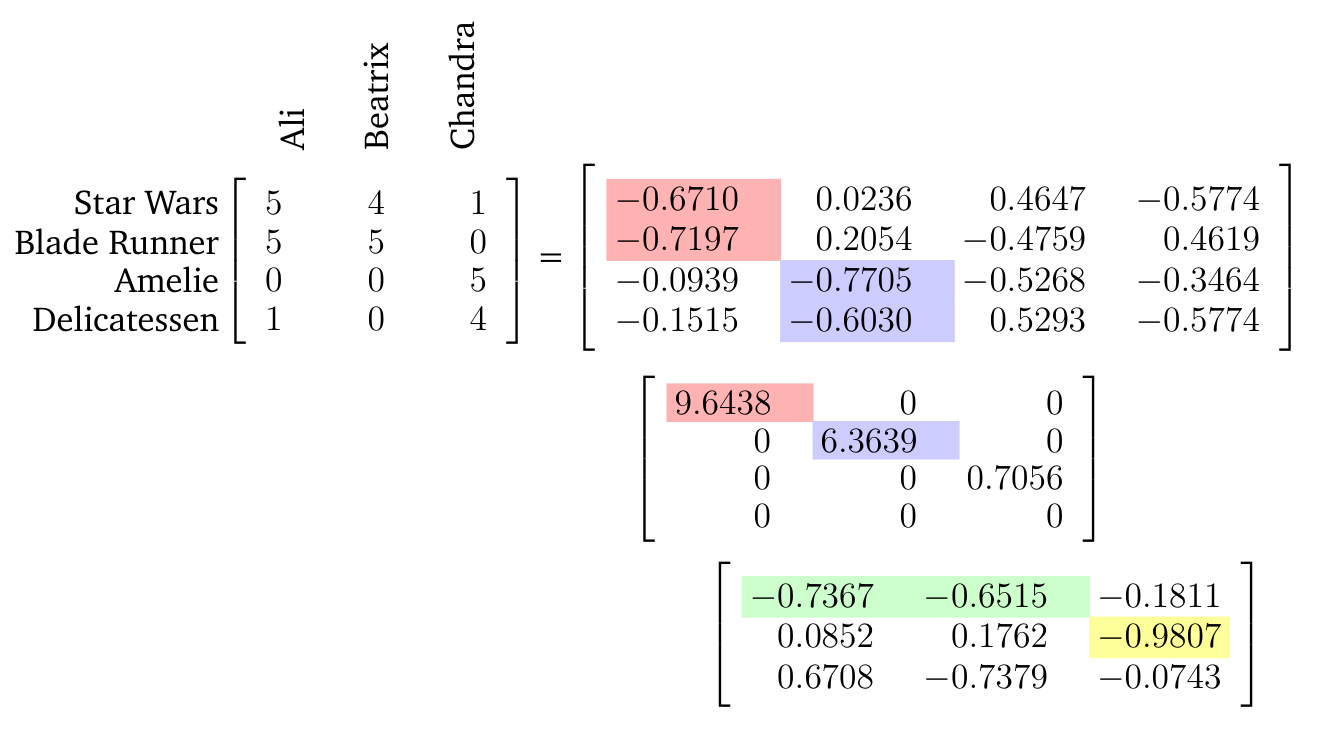
\includegraphics[width=0.92\textwidth,keepaspectratio]{docs/images/Figure4.10.png}
\caption*{\refstepcounter{figcounter}\label{fig:4-10}图~\thefigcounter 三个人对四部电影的评分及其对应的 SVD 分解。}
\end{figure}


\begin{notebox}
\textbf{例 4.14（在电影评分与消费者中发现结构）}
\end{notebox}

\begin{notebox}
我们通过分析人群及其偏好电影的数据，来为 SVD 补充一个实际的解释。考虑三位观众（Ali、Beatrix、Chandra）对四部不同电影（《星球大战》/ Star Wars、《银翼杀手》/ Blade Runner、《天使爱美丽》/ Amelie、《黑店狂想曲》/ Delicatessen）进行评分。他们的评分取值为 0（最差）到 5（最好）之间，并编码在数据矩阵 $ \boldsymbol{A} \in \mathbb{R}^{4 \times 3} $ 中，如图~\ref{fig:4-10} 所示。每一行代表一部电影，每一列代表一位用户。因此，电影评分的列向量（每位观众一个）为 $ \boldsymbol{x}_{\text{Ali}}, \boldsymbol{x}_{\text{Beatrix}}, \boldsymbol{x}_{\text{Chandra}} $。
\end{notebox}

\begin{notebox}
利用 SVD 分解 $ \boldsymbol{A} $ 为我们提供了一种捕捉人们如何对电影进行评分的关系的方法，尤其是是否存在某种结构将哪些人喜欢哪些电影联系起来。将 SVD 应用于我们的数据矩阵 $ \boldsymbol{A} $ 基于若干假设：

\begin{enumerate}
\item 所有观众都使用相同的线性映射一致地对电影进行评分。
\item 评分中不存在误差或噪声。
\item 我们将左奇异向量 $ \boldsymbol{u}_i $ 解释为典型电影（stereotypical movies），将右奇异向量 $ \boldsymbol{v}_j $ 解释为典型观众（stereotypical viewers）。
\end{enumerate}
\end{notebox}

\begin{notebox}
然后我们假设，任何观众的具体电影偏好都可以表示为 $ \boldsymbol{v}_j $ 的线性组合。类似地，任何电影的受欢迎程度都可以表示为 $ \boldsymbol{u}_i $ 的线性组合。因此，SVD 定义域中的一个向量可以解释为典型观众“空间”中的一位观众，而 SVD 到达域中的一个向量相应地可以解释为典型电影“空间”中的一部电影。（ \emph{边注} ：只有当数据本身涵盖了足够多样的观众和电影时，由相应观众和电影数据张成的这两个“空间”才具有实际意义。）让我们来考察电影-用户矩阵的 SVD 分解。第一个左奇异向量 $ \boldsymbol{u}_1 $ 在两部科幻电影上具有较大的绝对值，并且对应一个较大的第一奇异值（图~\ref{fig:4-10} 中的红色阴影）。因此，这把一类用户与一组特定的电影（科幻主题）关联起来。类似地，第一个右奇异向量 $ \boldsymbol{v}_1 $ 在 Ali 和 Beatrix 上的绝对值较大，这两位观众对科幻电影给出了很高的评分（图~\ref{fig:4-10} 中的绿色阴影）。这表明 $ \boldsymbol{v}_1 $ 反映了“科幻电影爱好者”的概念。
\end{notebox}

\begin{notebox}
类似地，$ \boldsymbol{u}_2 $ 似乎捕捉到了法国艺术电影的主题，而 $ \boldsymbol{v}_2 $ 表明 Chandra 接近此类电影的理想化爱好者。理想化的科幻电影爱好者是一位纯粹主义者，只喜欢科幻电影，因此科幻电影爱好者 $ \boldsymbol{v}_1 $ 对除了科幻主题之外的所有事物给出的评分均为零——这种逻辑由奇异值矩阵 $ \boldsymbol{\Sigma} $ 的对角子结构所体现。因此，一部具体的电影由它如何（线性地）分解为典型电影来表示。同样，一个人将由他们如何（通过线性组合）分解为电影主题来表示。
\end{notebox}

值得简要讨论一下 SVD 的术语和约定，因为文献中使用了不同的版本。数学原理在这些差异下保持不变，但这些差异可能会令人困惑。

为了在符号表示和抽象上带来便利，我们使用的 SVD 记号将 SVD 描述为具有两个方阵形式的左、右奇异向量矩阵，但具有一个长方形的奇异值矩阵。我们关于 SVD 的定义 (4.64) 有时被称为 \emph{完全 SVD（full SVD）} 。

一些作者对 SVD 的定义略有不同，并侧重于方阵形式的奇异矩阵。此时对于 $ \boldsymbol{A} \in \mathbb{R}^{m \times n} $ 且 $ m \ge n $：

\begin{equation}
\boldsymbol{A}_{m \times n} = \boldsymbol{U}_{m \times n} \boldsymbol{\Sigma}_{n \times n} \boldsymbol{V}^\top_{n \times n}
\tag{4.89}\label{eq:4-89}
\end{equation}

有时该表述被称为 \emph{简约 SVD（reduced SVD）} （例如 Datta (2010)）或直接称为 SVD（例如 Press et al. (2007)）。这种替代格式仅仅改变了矩阵的构建方式，但保持了 SVD 的数学结构不变。这种替代形式的便利之处在于 $ \boldsymbol{\Sigma} $ 是对角的，就像在特征值分解中一样。

在第 4.6 节中，我们将学习使用 SVD 的矩阵近似技术，这也被称为 \emph{截断 SVD（truncated SVD）} 。

我们可以对秩为 $ r $ 的矩阵 $ \boldsymbol{A} $ 定义 SVD，使得 $ \boldsymbol{U} $ 是 $ m \times r $ 矩阵，$ \boldsymbol{\Sigma} $ 是 $ r \times r $ 对角矩阵，而 $ \boldsymbol{V} $ 是 $ r \times n $ 矩阵。这种构造与我们的定义非常相似，并确保对角矩阵 $ \boldsymbol{\Sigma} $ 仅在对角线上具有非零元素。这种替代记号的主要便利之处在于 $ \boldsymbol{\Sigma} $ 是对角的，就像在特征值分解中一样。

要求 $ \boldsymbol{A} $ 的 SVD 仅适用于 $ m > n $ 的 $ m \times n $ 矩阵这一限制在实践中是不必要的。当 $ m < n $ 时，SVD 分解将产生列零向量多于行零向量的 $ \boldsymbol{\Sigma} $，因此奇异值 $ \sigma_{m+1}, \ldots, \sigma_n $ 均为 0。

SVD 在机器学习中具有广泛的应用，从曲线拟合中的最小二乘问题到求解线性方程组。这些应用利用了 SVD 的各种重要性质：它与矩阵秩的关系，以及它用较低秩的矩阵来近似给定秩矩阵的能力。用 SVD 替代矩阵通常具有使计算对数值舍入误差更加稳健的优点。正如我们将在下一节中探讨的那样，SVD 以原则性方式用“更简单”的矩阵来近似矩阵的能力，开启了从降维、主题建模到数据压缩和聚类等诸多机器学习应用的大门。

\section*{4.6 矩阵近似}
\addcontentsline{toc}{section}{4.6 矩阵近似}
\label{sec:4.6}

在第 4.5 节中，我们将 SVD 视为将矩阵 $ \boldsymbol{A} = \boldsymbol{U} \boldsymbol{\Sigma} \boldsymbol{V}^\top \in \mathbb{R}^{m \times n} $ 分解为三个矩阵的乘积的一种方法，其中 $ \boldsymbol{U} \in \mathbb{R}^{m \times m} $ 和 $ \boldsymbol{V} \in \mathbb{R}^{n \times n} $ 是正交矩阵，而 $ \boldsymbol{\Sigma} $ 的主对角线上包含奇异值。现在，我们不再进行完整的 SVD 分解，而是研究 SVD 如何使我们能够将矩阵 $ \boldsymbol{A} $ 表示为更简单的（低秩）矩阵 $ \boldsymbol{A}_i $ 之和，这自然引出了一种计算成本低于完整 SVD 的矩阵近似方案。

我们构造秩 1 矩阵 $ \boldsymbol{A}_i \in \mathbb{R}^{m \times n} $ 为

\begin{equation}
\boldsymbol{A}_i := \boldsymbol{u}_i \boldsymbol{v}_i^\top
\tag{4.90}\label{eq:4-90}
\end{equation}

它由 $ \boldsymbol{U} $ 和 $ \boldsymbol{V} $ 的第 $ i $ 个正交列向量的外积构成。图~\ref{fig:4-11} 展示了巨石阵（Stonehenge）的图像，该图像可以用矩阵 $ \boldsymbol{A} \in \mathbb{R}^{1432 \times 1910} $ 表示，并给出了如式~\eqref{eq:4-90} 中定义的若干外积 $ \boldsymbol{A}_i $。


\begin{figure}[H]
\centering
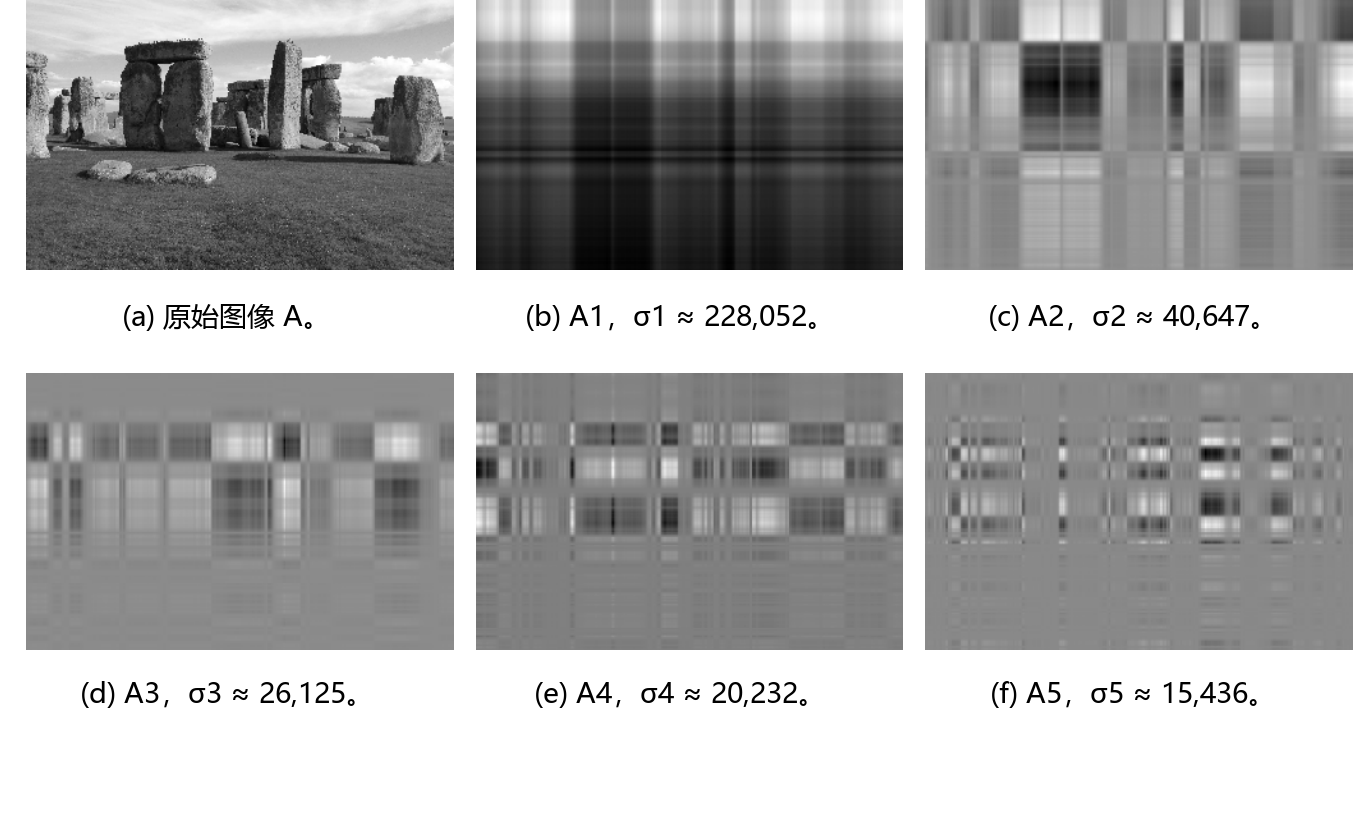
\includegraphics[width=0.92\textwidth,keepaspectratio]{docs/images/Figure4.11.png}
\caption*{\refstepcounter{figcounter}\label{fig:4-11}图~\thefigcounter 使用 SVD 进行图像处理。(a) 原始灰度图像是一个取值在 0（黑）到 1（白）之间的 1432 × 1910 矩阵。(b)–(f) 秩 1 矩阵 A₁ 至 A₅ 及其对应的奇异值 σ₁ 至 σ₅。每个秩 1 矩阵的网格状结构是由左奇异向量与右奇异向量的外积决定的。}
\end{figure}


秩为 $ r $ 的矩阵 $ \boldsymbol{A} \in \mathbb{R}^{m \times n} $ 可以写为秩 1 矩阵 $ \boldsymbol{A}_i $ 之和：

\begin{equation}
\boldsymbol{A} = \sum_{i=1}^r \sigma_i \boldsymbol{u}_i \boldsymbol{v}_i^\top = \sum_{i=1}^r \sigma_i \boldsymbol{A}_i
\tag{4.91}\label{eq:4-91}
\end{equation}

其中外积矩阵 $ \boldsymbol{A}_i $ 由第 $ i $ 个奇异值 $ \sigma_i $ 进行加权。我们可以看出为什么式~\eqref{eq:4-91} 成立：奇异值矩阵 $ \boldsymbol{\Sigma} $ 的对角结构仅将相匹配的左、右奇异向量 $ \boldsymbol{u}_i \boldsymbol{v}_i^\top $ 相乘，并乘以相应的奇异值 $ \sigma_i $ 进行缩放。当 $ i \neq j $ 时，由于 $ \boldsymbol{\Sigma} $ 是对角矩阵，所有项 $ \Sigma_{ij} \boldsymbol{u}_i \boldsymbol{v}_j^\top $ 都为零。当 $ i > r $ 时，由于对应的奇异值均为 0，所有项也都为零。

在式~\eqref{eq:4-90} 中，我们引入了秩 1 矩阵 $ \boldsymbol{A}_i $。我们将 $ r $ 个独立的秩 1 矩阵相加得到了秩为 $ r $ 的矩阵 $ \boldsymbol{A} $；参见式~\eqref{eq:4-91}。如果求和不遍历所有矩阵 $ \boldsymbol{A}_i $（$ i = 1, \ldots, r $），而是仅累加到某个中间值 $ k < r $，我们就得到了 $ \boldsymbol{A} $ 的一个 \emph{秩 $ k $ 近似（rank-$ k $ approximation）} ：

\begin{equation}
\widehat{\boldsymbol{A}}(k) := \sum_{i=1}^k \sigma_i \boldsymbol{u}_i \boldsymbol{v}_i^\top = \sum_{i=1}^k \sigma_i \boldsymbol{A}_i
\tag{4.92}\label{eq:4-92}
\end{equation}

满足 $ \text{rk}(\widehat{\boldsymbol{A}}(k)) = k $。图~\ref{fig:4-12} 展示了巨石阵原始图像 $ \boldsymbol{A} $ 的低秩近似 $ \widehat{\boldsymbol{A}}(k) $。在秩 5 近似中，巨石的形状变得越来越清晰且容易辨认。原始图像需要存储 $ 1432 \times 1910 = 2735120 $ 个数值，而秩 5 近似仅需我们存储 5 个奇异值以及 5 个左、右奇异向量（维度分别为 1432 和 1910），总共只需 $ 5 \times (1432 + 1910 + 1) = 16715 $ 个数值——仅略高于原始数据的 0.6\%。


\begin{figure}[H]
\centering
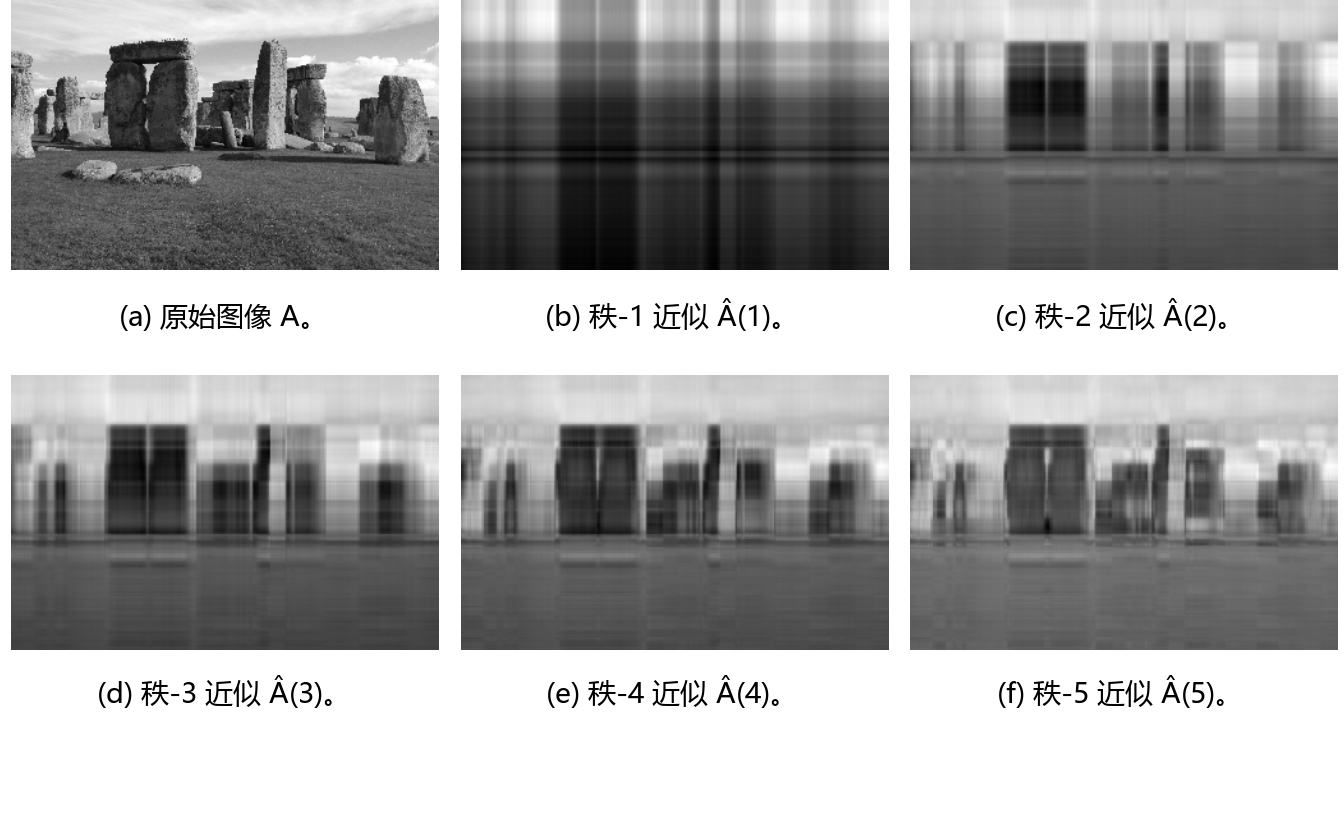
\includegraphics[width=0.92\textwidth,keepaspectratio]{docs/images/Figure4.12.png}
\caption*{\refstepcounter{figcounter}\label{fig:4-12}图~\thefigcounter 使用 SVD 进行图像重构。(a) 原始图像。(b)–(f) 使用 SVD 的低秩近似进行图像重构，其中秩 k 近似由 Â(k) = ∑\_\{i=1\}\textasciicircum{}k σᵢ Aᵢ 给出。}
\end{figure}


为了度量 $ \boldsymbol{A} $ 与其秩 $ k $ 近似 $ \widehat{\boldsymbol{A}}(k) $ 之间的差异（误差），我们需要范数的概念。在第 3.1 节中，我们已经使用了用于度量向量长度的向量范数。类似地，我们也可以在矩阵上定义范数。

\textbf{定义 4.23}（矩阵的谱范数）。对于 $ \boldsymbol{x} \in \mathbb{R}^n \setminus \{\boldsymbol{0}\} $，矩阵 $ \boldsymbol{A} \in \mathbb{R}^{m \times n} $ 的 \emph{谱范数（spectral norm）} 定义为：

\begin{equation}
\|\boldsymbol{A}\|_2 := \max_{\boldsymbol{x}} \frac{\|\boldsymbol{A} \boldsymbol{x}\|_2}{\|\boldsymbol{x}\|_2}
\tag{4.93}\label{eq:4-93}
\end{equation}

我们在矩阵范数（左侧）中引入了下标记号，类似于具有下标 2 的向量欧几里得范数（右侧）。谱范数 (4.93) 决定了任意向量 $ \boldsymbol{x} $ 在与 $ \boldsymbol{A} $ 相乘后所能达到的最大长度。

\textbf{定理 4.24}。矩阵 $ \boldsymbol{A} $ 的谱范数是其最大奇异值 $ \sigma_1 $。

我们将该定理的证明留作练习。

\textbf{定理 4.25}（Eckart-Young 定理（Eckart and Young, 1936））。考虑秩为 $ r $ 的矩阵 $ \boldsymbol{A} \in \mathbb{R}^{m \times n} $，并设 $ \boldsymbol{B} \in \mathbb{R}^{m \times n} $ 为秩为 $ k $ 的矩阵。对于任意 $ k \leqslant r $，记 $ \widehat{\boldsymbol{A}}(k) = \sum_{i=1}^k \sigma_i \boldsymbol{u}_i \boldsymbol{v}_i^\top $，则有：

\begin{equation}
\widehat{\boldsymbol{A}}(k) = \arg\min_{\text{rk}(\boldsymbol{B}) = k} \|\boldsymbol{A} - \boldsymbol{B}\|_2
\tag{4.94}\label{eq:4-94}
\end{equation}

\begin{equation}
\|\boldsymbol{A} - \widehat{\boldsymbol{A}}(k)\|_2 = \sigma_{k+1}
\tag{4.95}\label{eq:4-95}
\end{equation}

Eckart-Young 定理明确给出了利用秩 $ k $ 近似来近似 $ \boldsymbol{A} $ 所引入的误差大小。我们可以将通过 SVD 获得的秩 $ k $ 近似解释为将满秩矩阵 $ \boldsymbol{A} $ 投影到由秩至多为 $ k $ 的矩阵所构成的低维空间上。在所有可能的投影中，SVD 使得 $ \boldsymbol{A} $ 与任意秩 $ k $ 近似之间的误差（关于谱范数）达到最小。

我们可以回顾一些推导步骤以理解式~\eqref{eq:4-95} 为什么成立。我们注意到差值 $ \boldsymbol{A} - \widehat{\boldsymbol{A}}(k) $ 是包含剩余秩 1 矩阵之和的矩阵：

\begin{equation}
\boldsymbol{A} - \widehat{\boldsymbol{A}}(k) = \sum_{i=k+1}^r \sigma_i \boldsymbol{u}_i \boldsymbol{v}_i^\top
\tag{4.96}\label{eq:4-96}
\end{equation}

根据定理 4.24，我们立即得到差值矩阵的谱范数为 $ \sigma_{k+1} $。现在我们更仔细地考察式~\eqref{eq:4-94}。假设存在另一个秩满足 $ \text{rk}(\boldsymbol{B}) \leqslant k $ 的矩阵 $ \boldsymbol{B} $，使得：

\begin{equation}
\|\boldsymbol{A} - \boldsymbol{B}\|_2 < \|\boldsymbol{A} - \widehat{\boldsymbol{A}}(k)\|_2
\tag{4.97}\label{eq:4-97}
\end{equation}

则存在一个至少为 $ (n - k) $ 维的零空间 $ Z \subseteq \mathbb{R}^n $，使得对任意 $ \boldsymbol{x} \in Z $ 均有 $ \boldsymbol{B} \boldsymbol{x} = \boldsymbol{0} $。由此可得：

\begin{equation}
\|\boldsymbol{A} \boldsymbol{x}\|_2 = \|(\boldsymbol{A} - \boldsymbol{B})\boldsymbol{x}\|_2
\tag{4.98}\label{eq:4-98}
\end{equation}

再利用包含矩阵范数形式的柯西-施瓦茨不等式（式~\eqref{eq:3-17}），我们得到：

\begin{equation}
\|\boldsymbol{A} \boldsymbol{x}\|_2 \leqslant \|\boldsymbol{A} - \boldsymbol{B}\|_2 \|\boldsymbol{x}\|_2 < \sigma_{k+1} \|\boldsymbol{x}\|_2
\tag{4.99}\label{eq:4-99}
\end{equation}

然而，存在一个由 $ \boldsymbol{A} $ 的右奇异向量 $ \boldsymbol{v}_j $（$ j \leqslant k + 1 $）张成的 $ (k + 1) $ 维子空间，在该子空间上满足 $ \|\boldsymbol{A} \boldsymbol{x}\|_2 \geqslant \sigma_{k+1} \|\boldsymbol{x}\|_2 $。将这两个空间的维度相加得到的数值大于 $ n $，因此这两个空间中必然存在一个非零公共向量。这与第 2.7.3 节中的秩-零度定理（定理 2.24）相矛盾。

Eckart-Young 定理表明，我们可以利用 SVD 以一种有原则且最优（在谱范数意义下）的方式将秩为 $ r $ 的矩阵 $ \boldsymbol{A} $ 降至秩为 $ k $ 的矩阵 $ \widehat{\boldsymbol{A}} $。我们可以将由秩 $ k $ 矩阵对 $ \boldsymbol{A} $ 的近似解释为一种有损压缩形式。因此，矩阵的低秩近似出现在许多机器学习应用中，例如图像处理、噪声滤波以及病态问题的正则化。此外，正如我们将在第 10 章中看到的，它在降维和主成分分析中也发挥着关键作用。

\begin{notebox}
\textbf{例 4.15（在电影评分与消费者中寻找结构（续））}
\end{notebox}

\begin{notebox}
回到我们的电影评分示例，我们现在可以应用低秩近似的概念来近似原始数据矩阵。回顾可知，我们的第一个奇异值刻画了电影中的科幻主题和科幻迷的概念。因此，在电影评分矩阵的秩 1 分解中仅使用第一个奇异值项，我们得到预测评分：

\begin{equation}
\boldsymbol{A}_1 = \boldsymbol{u}_1 \boldsymbol{v}_1^\top = \begin{bmatrix} -0.6710 \\ -0.7197 \\ -0.0939 \\ -0.1515 \end{bmatrix} \begin{bmatrix} -0.7367 & -0.6515 & -0.1811 \end{bmatrix}
\tag{4.100a}\label{eq:4-100a}
\end{equation}

\begin{equation}
= \begin{bmatrix} 0.4943 & 0.4372 & 0.1215 \\ 0.5302 & 0.4689 & 0.1303 \\ 0.0692 & 0.0612 & 0.0170 \\ 0.1116 & 0.0987 & 0.0274 \end{bmatrix}
\tag{4.100b}\label{eq:4-100b}
\end{equation}

这一秩 1 近似 $ \boldsymbol{A}_1 $ 非常富有启发性：它告诉我们 Ali 和 Beatrix 喜欢科幻电影，如《星球大战》（Star Wars）和《银翼杀手》（Blade Runner）（各项数值大于 4），但未能刻画 Chandra 对其他电影的评分。这并不奇怪，因为 Chandra 喜欢的电影类型并未被第一个奇异值所捕获。第二个奇异值则为这些电影主题的爱好者提供了更好的秩 1 近似：

\begin{equation}
\boldsymbol{A}_2 = \boldsymbol{u}_2 \boldsymbol{v}_2^\top = \begin{bmatrix} 0.0236 \\ 0.2054 \\ -0.7705 \\ -0.6030 \end{bmatrix} \begin{bmatrix} 0.0852 & 0.1762 & -0.9807 \end{bmatrix}
\tag{4.101a}\label{eq:4-101a}
\end{equation}

\begin{equation}
= \begin{bmatrix} -0.0154 & 0.0042 & -0.0174 \\ -0.1338 & 0.0362 & -0.1516 \\ 0.5019 & -0.1358 & 0.5686 \\ 0.3928 & -0.1063 & 0.4450 \end{bmatrix}
\tag{4.101b}\label{eq:4-101b}
\end{equation}

在这第二个秩 1 近似 $ \boldsymbol{A}_2 $ 中，我们很好地捕获了 Chandra 的评分和电影类型，但没有捕获科幻电影。这促使我们考虑秩 2 近似 $ \widehat{\boldsymbol{A}}(2) $，我们将前两个秩 1 近似组合起来：

\begin{equation}
\begin{adjustbox}{max width=\linewidth}
\widehat{\boldsymbol{A}}(2) = \sigma_1 \boldsymbol{A}_1 + \sigma_2 \boldsymbol{A}_2 = \begin{bmatrix} 4.7801 & 4.2419 & 1.0244 \\ 5.2252 & 4.7522 & -0.0250 \\ 0.2493 & -0.2743 & 4.9724 \\ 0.7495 & 0.2756 & 4.0278 \end{bmatrix}
\end{adjustbox}
\tag{4.102}\label{eq:4-102}
\end{equation}

$ \widehat{\boldsymbol{A}}(2) $ 与原始电影评分表非常相似：

\begin{equation}
\boldsymbol{A} = \begin{bmatrix} 5 & 4 & 1 \\ 5 & 5 & 0 \\ 0 & 0 & 5 \\ 1 & 0 & 4 \end{bmatrix}
\tag{4.103}\label{eq:4-103}
\end{equation}

这表明我们可以忽略 $ \boldsymbol{A}_3 $ 的贡献。我们可以将其解释为：在数据表中没有证据表明存在第三种电影主题/电影爱好者类别。这也意味着在我们的示例中，电影主题/电影爱好者的整个空间是一个由科幻电影和法国艺术电影及其爱好者张成的二维空间。
\end{notebox}

\section*{4.7 矩阵谱系}
\addcontentsline{toc}{section}{4.7 矩阵谱系}
\label{sec:4.7}

\emph{备注} 。“系统发育/谱系（phylogenetic）”一词描述了我们如何刻画个体或群体之间的亲缘关系，源自希腊语中表示“部族”和“来源”的词汇。♦

在第 2 章和第 3 章中，我们介绍了线性代数和解析几何的基础知识。在本章中，我们探讨了矩阵和线性映射的基本特征。图~\ref{fig:4-13} 描绘了不同类型矩阵之间关系的谱系树（黑色箭头表示“是……的子集”），以及我们可以对它们执行的各项讨论过的运算（蓝色表示）。我们考虑所有实矩阵 $ \boldsymbol{A} \in \mathbb{R}^{n \times m} $。对于非方阵（其中 $ n \neq m $），正如我们在本章中所见，SVD 总是存在的。聚焦于方阵 $ \boldsymbol{A} \in \mathbb{R}^{n \times n} $，行列式可以告诉我们方阵是否拥有逆矩阵，即它是否属于正则、可逆矩阵类。如果该 $ n \times n $ 方阵拥有 $ n $ 个线性无关的特征向量，则该矩阵是非亏损的，并且存在特征分解（定理 4.12）。我们知道，重特征值可能导致亏损矩阵，而亏损矩阵是无法对角化的。

非奇异矩阵与非亏损矩阵并不相同。例如，旋转矩阵是可逆的（行列式非零），但在实数范围内不可对角化（其特征值不能保证是实数）。


\begin{figure}[H]
\centering
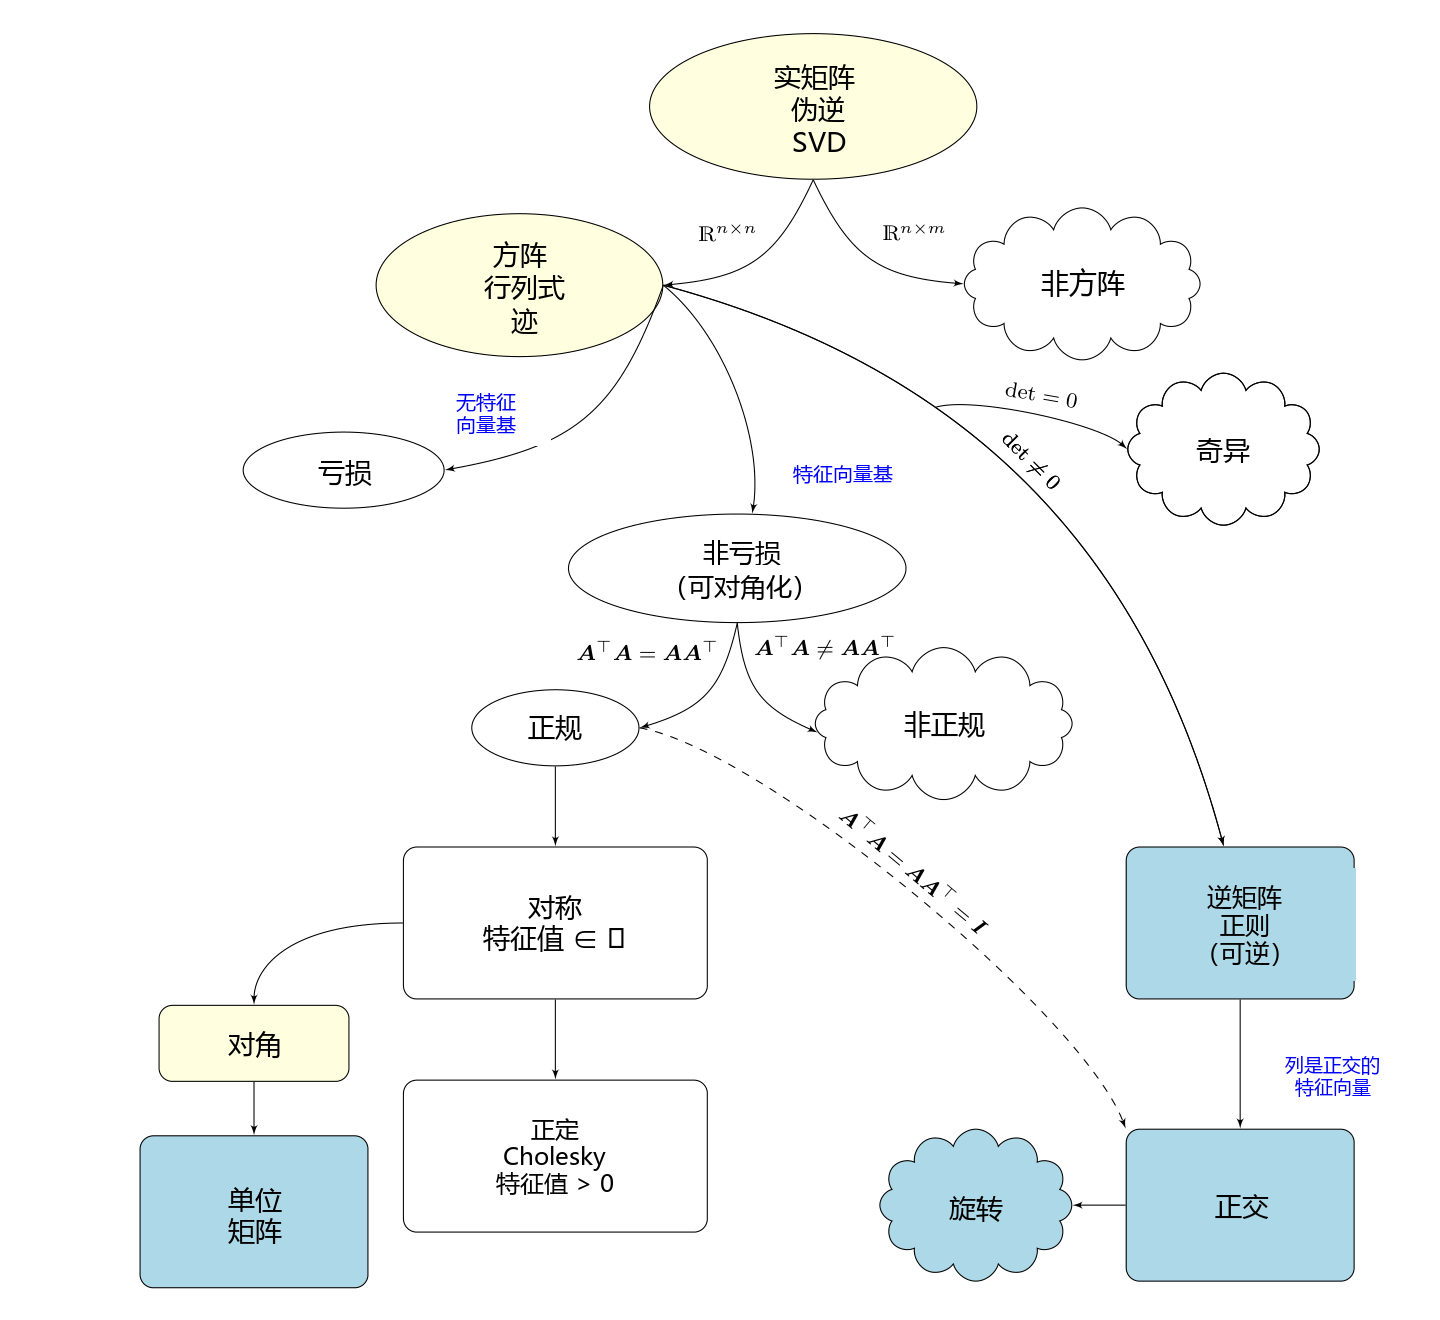
\includegraphics[width=0.92\textwidth,keepaspectratio]{docs/images/Figure4.13.png}
\caption*{\refstepcounter{figcounter}\label{fig:4-13}图~\thefigcounter 机器学习中遇到的矩阵的功能分类谱系树。}
\end{figure}


我们进一步深入非亏损 $ n \times n $ 方阵的分支。如果条件 $ \boldsymbol{A}^\top \boldsymbol{A} = \boldsymbol{A} \boldsymbol{A}^\top $ 成立，则 $ \boldsymbol{A} $ 是 \emph{正规（normal）} 矩阵。此外，如果满足更严格的条件 $ \boldsymbol{A}^\top \boldsymbol{A} = \boldsymbol{A} \boldsymbol{A}^\top = \boldsymbol{I} $，则称 $ \boldsymbol{A} $ 为 \emph{正交（orthogonal）} 矩阵（参见定义 3.8）。正交矩阵的集合是正则（可逆）矩阵的子集，且满足 $ \boldsymbol{A}^\top = \boldsymbol{A}^{-1} $。

正规矩阵包含一个经常遇到的子集——对称矩阵 $ \boldsymbol{S} \in \mathbb{R}^{n \times n} $，其满足 $ \boldsymbol{S} = \boldsymbol{S}^\top $。对称矩阵只有实特征值。对称矩阵的一个子集由正定矩阵 $ \boldsymbol{P} $ 组成，满足对于所有 $ \boldsymbol{x} \in \mathbb{R}^n \setminus \{\boldsymbol{0}\} $ 都有 $ \boldsymbol{x}^\top \boldsymbol{P} \boldsymbol{x} > 0 $。在这种情形下，存在唯一的 Cholesky 分解（定理 4.18）。正定矩阵只有正特征值，并且总是可逆的（即具有非零行列式）。

对称矩阵的另一个子集是对角矩阵 $ \boldsymbol{D} $。对角矩阵在乘法和加法下是封闭的，但不一定构成群（仅当所有对角元素均非零使得矩阵可逆时才构成群）。一个特殊的对角矩阵是单位矩阵 $ \boldsymbol{I} $。

\section*{4.8 延伸阅读}
\addcontentsline{toc}{section}{4.8 延伸阅读}
\label{sec:4.8}

本章的大部分内容建立了基础数学知识，并将其与研究映射的方法联系起来，其中许多方法位于机器学习的核心地位，是支撑软件解决方案以及几乎所有机器学习理论的基石。利用行列式、特征谱和特征空间对矩阵进行表征，为矩阵的分类与分析提供了基本特征和判定条件。这不仅适用于所有形式的数据表示以及涉及数据的映射，还可以用于评估对此类矩阵进行计算操作时的数值稳定性 (Press et al., 2007)。

行列式是“手算”求逆矩阵和计算特征值的基础工具。然而，对于除了最小规模实例之外的几乎所有情形，利用高斯消元法的数值计算性能都优于行列式 (Press et al., 2007)。尽管如此，行列式仍然是一个强大的理论概念，例如可以根据行列式的符号来获得关于基定向的直观理解。特征向量可用于执行基变换，将数据转换到具有实际意义的正交特征向量坐标系中。类似地，矩阵分解方法（如 Cholesky 分解）在计算或模拟随机事件时经常出现 (Rubinstein and Kroese, 2016)。因此，Cholesky 分解使我们能够计算重参数化技巧（reparametrization trick），这在我们希望对随机变量执行连续求导时非常有用，例如在变分自编码器中 (Jimenez Rezende et al., 2014; Kingma and Ba, 2014)。

特征分解对于使我们能够提取表征线性映射的有意义且可解释的信息至关重要。因此，特征分解是被称为 \emph{谱方法（spectral methods）} 的一类通用机器学习算法的基础，这类算法对正定核执行特征分解。这些谱分解方法涵盖了统计数据分析的经典方法，例如：

\begin{itemize}
\item \emph{主成分分析（principal component analysis, PCA）} (Pearson, 1901; 另见第 10 章)，其中寻求一个解释数据中大部分变异性的低维子空间。
\item \emph{Fisher 判别分析（Fisher discriminant analysis）} ，旨在确定用于数据分类的分离超平面 (Mika et al., 1999)。
\item \emph{多维标度法（multidimensional scaling, MDS）} (Carroll and Chang, 1970)。
\end{itemize}

这些方法的计算效率通常来自于寻找对称半正定矩阵的最佳秩 $ k $ 近似。谱方法的更现代示例具有不同的渊源，但它们每一个都需要计算正定核的特征向量和特征值，例如 \emph{Isomap} (Tenenbaum et al., 2000)、 \emph{拉普拉斯特征映射（Laplacian eigenmaps）} (Belkin and Niyogi, 2003)、 \emph{Hessian 特征映射（Hessian eigenmaps）} (Donoho and Grimes, 2003) 以及 \emph{谱聚类（spectral clustering）} (Shi and Malik, 2000)。这些方法的核心计算通常由低秩矩阵近似技术支撑 (Belabbas and Wolfe, 2009)，正如我们在此处通过 SVD 所了解到的那样。

SVD 使我们能够发现与特征分解相同类型的某些信息。然而，SVD 更普遍地适用于非方阵和数据表。每当我们希望识别数据中的异质性、通过近似进行数据压缩（例如，仅存储 $ (n + m)k $ 个数值而不是存储 $ n \times m $ 个数值），或者希望进行数据预处理（例如消除设计矩阵中预测变量的相关性 (Ormoneit et al., 2001)）时，这些矩阵因子分解方法都会发挥作用。SVD 作用于矩阵，我们可以将矩阵解释为带有两个索引（行和列）的矩形数组。将类似矩阵的结构推广到更高维度的数组被称为 \emph{张量（tensors）} 。事实证明，SVD 只是作用于此类张量的更一般分解族的一个特例 (Kolda and Bader, 2009)。张量上的类似 SVD 的操作和低秩近似包括例如 \emph{Tucker 分解（Tucker decomposition）} (Tucker, 1966) 或 \emph{CP 分解（CP decomposition）} (Carroll and Chang, 1970)。

出于计算效率的考虑，SVD 低秩近似在机器学习中被频繁使用。这是因为它减少了我们在潜在的极大实际数据矩阵上所需执行的内存占用以及非零乘法运算次数 (Trefethen and Bau III, 1997)。此外，低秩近似还用于处理可能包含缺失值的矩阵，以及用于有损压缩和降维的目的 (Moonen and De Moor, 1995; Markovsky, 2011)。

\chapter*{练习}
\addcontentsline{toc}{section}{练习}

\section*{练习 5.1}
\addcontentsline{toc}{subsection}{练习 5.1}

计算下列函数的导数 $ f'(x) $：

\begin{equation*}
f(x) = \log(x^4) \sin(x^3)
\end{equation*}

\medskip\hrule\medskip

\section*{练习 5.2}
\addcontentsline{toc}{subsection}{练习 5.2}

计算 Logistic Sigmoid 函数：

\begin{equation*}
f(x) = \frac{1}{1 + \exp(-x)}
\end{equation*}

的导数 $ f'(x) $。

\medskip\hrule\medskip

\section*{练习 5.3}
\addcontentsline{toc}{subsection}{练习 5.3}

计算函数：

\begin{equation*}
f(x) = \exp\left(-\frac{1}{2\sigma^2} (x - \mu)^2\right)
\end{equation*}

的导数 $ f'(x) $，其中 $ \mu, \sigma \in \mathbb{R} $ 为常数。

\medskip\hrule\medskip

\section*{练习 5.4}
\addcontentsline{toc}{subsection}{练习 5.4}

计算函数 $ f(x) = \sin(x) + \cos(x) $ 在 $ x_0 = 0 $ 处的泰勒多项式 $ T_n $（$ n = 0, \ldots, 5 $）。

\medskip\hrule\medskip

\section*{练习 5.5}
\addcontentsline{toc}{subsection}{练习 5.5}

考虑下列函数：

\begin{equation*}
f_1(\boldsymbol{x}) = \sin(x_1) \cos(x_2), \quad \boldsymbol{x} \in \mathbb{R}^2
\end{equation*}

\begin{equation*}
f_2(\boldsymbol{x}, \boldsymbol{y}) = \boldsymbol{x}^\top \boldsymbol{y}, \quad \boldsymbol{x}, \boldsymbol{y} \in \mathbb{R}^n
\end{equation*}

\begin{equation*}
f_3(\boldsymbol{x}) = \boldsymbol{x} \boldsymbol{x}^\top, \quad \boldsymbol{x} \in \mathbb{R}^n
\end{equation*}

a. $ \frac{\partial f_i}{\partial \boldsymbol{x}} $ 的维度分别是什么？ b. 计算对应的雅可比矩阵（Jacobians）。

\medskip\hrule\medskip

\section*{练习 5.6}
\addcontentsline{toc}{subsection}{练习 5.6}

求 $ f $ 关于 $ \boldsymbol{t} $ 的导数以及 $ g $ 关于 $ \boldsymbol{X} $ 的导数，其中：

\begin{equation*}
f(\boldsymbol{t}) = \sin(\log(\boldsymbol{t}^\top \boldsymbol{t})), \quad \boldsymbol{t} \in \mathbb{R}^D
\end{equation*}

\begin{equation*}
\begin{adjustbox}{max width=\linewidth}
g(\boldsymbol{X}) = \operatorname{tr}(\boldsymbol{A} \boldsymbol{X} \boldsymbol{B}), \quad \boldsymbol{A} \in \mathbb{R}^{D \times E}, \; \boldsymbol{X} \in \mathbb{R}^{E \times F}, \; \boldsymbol{B} \in \mathbb{R}^{F \times D}
\end{adjustbox}
\end{equation*}

其中 $ \operatorname{tr} $ 表示矩阵的迹。

\medskip\hrule\medskip

\section*{练习 5.7}
\addcontentsline{toc}{subsection}{练习 5.7}

利用链式法则计算下列函数的导数 $ \frac{\mathrm{d}f}{\mathrm{d}\boldsymbol{x}} $。给出每个偏导数的维度，并详细描述你的推导步骤。

a.

\begin{equation*}
f(z) = \log(1 + z), \quad z = \boldsymbol{x}^\top \boldsymbol{x}, \quad \boldsymbol{x} \in \mathbb{R}^D
\end{equation*}

b.

\begin{equation*}
\begin{adjustbox}{max width=\linewidth}
f(\boldsymbol{z}) = \sin(\boldsymbol{z}), \quad \boldsymbol{z} = \boldsymbol{A} \boldsymbol{x} + \boldsymbol{b}, \quad \boldsymbol{A} \in \mathbb{R}^{E \times D}, \; \boldsymbol{x} \in \mathbb{R}^D, \; \boldsymbol{b} \in \mathbb{R}^E
\end{adjustbox}
\end{equation*}

其中 $ \sin(\cdot) $ 逐元素作用于 $ \boldsymbol{z} $。

\medskip\hrule\medskip

\section*{练习 5.8}
\addcontentsline{toc}{subsection}{练习 5.8}

计算下列函数的导数 $ \frac{\mathrm{d}f}{\mathrm{d}\boldsymbol{x}} $。详细描述你的推导步骤。

a. 使用链式法则。给出每个偏导数的维度。

\begin{equation*}
f(z) = \exp\left(-\frac{1}{2} z\right)
\end{equation*}

\begin{equation*}
z = g(\boldsymbol{y}) = \boldsymbol{y}^\top \boldsymbol{S}^{-1} \boldsymbol{y}
\end{equation*}

\begin{equation*}
\boldsymbol{y} = h(\boldsymbol{x}) = \boldsymbol{x} - \boldsymbol{\mu}
\end{equation*}

其中 $ \boldsymbol{x}, \boldsymbol{\mu} \in \mathbb{R}^D $，$ \boldsymbol{S} \in \mathbb{R}^{D \times D} $。

b.

\begin{equation*}
f(\boldsymbol{x}) = \operatorname{tr}(\boldsymbol{x} \boldsymbol{x}^\top + \sigma^2 \boldsymbol{I}), \quad \boldsymbol{x} \in \mathbb{R}^D
\end{equation*}

这里 $ \operatorname{tr}(\boldsymbol{A}) $ 是 $ \boldsymbol{A} $ 的迹，即对角线元素之和 $ \sum_i A_{ii} $。提示：显式写出外积。

c. 使用链式法则。给出每个偏导数的维度。不需要显式计算偏导数的乘积。

\begin{equation*}
\boldsymbol{f} = \tanh(\boldsymbol{z}) \in \mathbb{R}^M
\end{equation*}

\begin{equation*}
\boldsymbol{z} = \boldsymbol{A} \boldsymbol{x} + \boldsymbol{b}, \quad \boldsymbol{x} \in \mathbb{R}^N, \; \boldsymbol{A} \in \mathbb{R}^{M \times N}, \; \boldsymbol{b} \in \mathbb{R}^M
\end{equation*}

这里，$ \tanh $ 逐分量作用于 $ \boldsymbol{z} $。

\medskip\hrule\medskip

\section*{练习 5.9}
\addcontentsline{toc}{subsection}{练习 5.9}

对于可微函数 $ p, q, t $，我们定义：

\begin{equation*}
g(z, \nu) := \log p(x, z) - \log q(z, \nu)
\end{equation*}

\begin{equation*}
z := t(\epsilon, \nu)
\end{equation*}

利用链式法则，计算梯度：

\begin{equation*}
\frac{\mathrm{d}}{\mathrm{d}\nu} g(z, \nu)
\end{equation*}

\chapter{5 向量微积分}

机器学习中的许多算法都通过针对一组期望的模型参数优化目标函数来控制模型对数据的解释程度：寻找良好参数的过程可以表述为一个优化问题（参见第 8.2 节和第 8.3 节）。示例包括：(i) 线性回归（参见第 9 章），其中我们研究曲线拟合问题，并通过优化线性权重参数来最大化似然；(ii) 用于降维和数据压缩的神经网络自编码器，其中的参数是每一层的权重与偏置，我们通过反复应用链式法则来最小化重构误差；(iii) 用于对数据分布进行建模的高斯混合模型（参见第 11 章），其中我们优化每个混合分量的位置与形状参数以最大化模型的似然。图~\ref{fig:5-1} 说明了其中的一些问题，我们通常利用利用梯度信息的优化算法（第 7.1 节）来求解这些问题。图~\ref{fig:5-2} 概述了本章各个概念之间的关系，以及它们与本书其他章节的联系。


\begin{figure}[H]
\centering
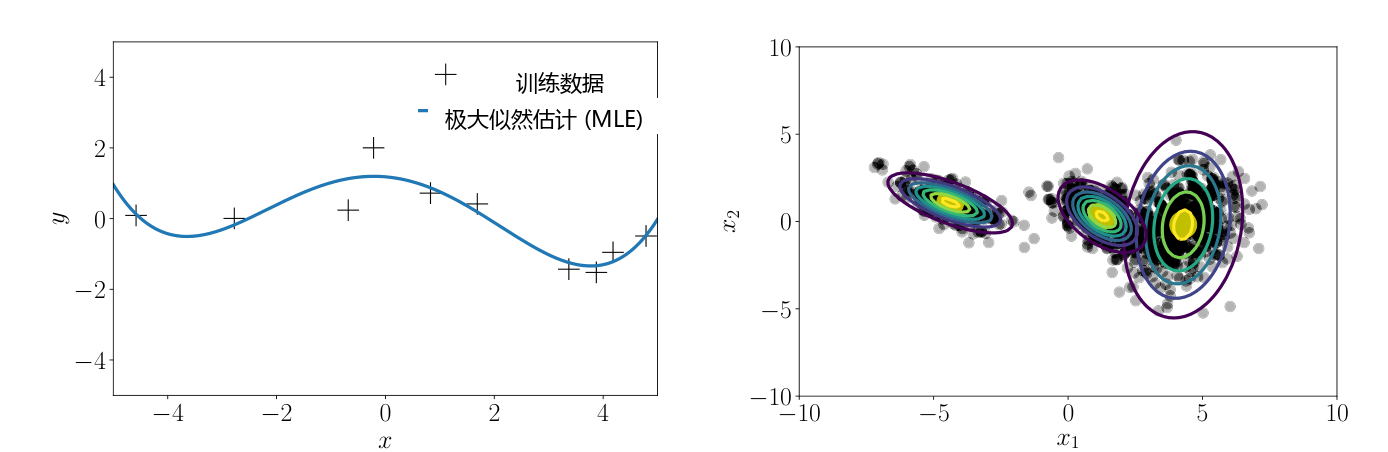
\includegraphics[width=0.92\textwidth,keepaspectratio]{docs/images/Figure5.1.png}
\caption*{\refstepcounter{figcounter}\label{fig:5-1}图~\thefigcounter 向量微积分在 (a) 回归（曲线拟合）和 (b) 密度估计（即数据分布建模）中起着核心作用。}
\end{figure}


本章的核心是函数的概念。函数 $ f $ 是将两个量联系起来的量。在本书中，这些量通常是输入 $ \boldsymbol{x} \in \mathbb{R}^D $ 和目标（函数值）$ f(\boldsymbol{x}) $，若无特殊说明，我们假定它们是实值的。这里 $ \mathbb{R}^D $ 是 $ f $ 的 \emph{定义域（domain）} ，而函数值 $ f(\boldsymbol{x}) $ 是 $ f $ 的 \emph{像/到达域（image/codomain）} 。第 2.7.3 节在线性函数背景下提供了更详细的讨论。我们经常写作：

\begin{equation}
f : \mathbb{R}^D \to \mathbb{R}
\tag{5.1a}\label{eq:5-1a}
\end{equation}

\begin{equation}
\boldsymbol{x} \mapsto f(\boldsymbol{x})
\tag{5.1b}\label{eq:5-1b}
\end{equation}

来指明一个函数，其中式~\eqref{eq:5-1a} 指定 $ f $ 是从 $ \mathbb{R}^D $ 到 $ \mathbb{R} $ 的映射，而式~\eqref{eq:5-1b} 指定了将输入 $ \boldsymbol{x} $ 显式对应到函数值 $ f(\boldsymbol{x}) $。函数 $ f $ 为每个输入 $ \boldsymbol{x} $ 分配唯一的函数值 $ f(\boldsymbol{x}) $。

\begin{notebox}
\textbf{例 5.1}
\end{notebox}

\begin{notebox}
回想作为内积特例的点积（第 3.2 节）。在上述记号下，函数 $ f(\boldsymbol{x}) = \boldsymbol{x}^\top \boldsymbol{x} $（$ \boldsymbol{x} \in \mathbb{R}^2 $）可表示为：

\begin{equation}
f : \mathbb{R}^2 \to \mathbb{R}
\tag{5.2a}\label{eq:5-2a}
\end{equation}

\begin{equation}
\boldsymbol{x} \mapsto x_1^2 + x_2^2
\tag{5.2b}\label{eq:5-2b}
\end{equation}
\end{notebox}


\begin{figure}[H]
\centering
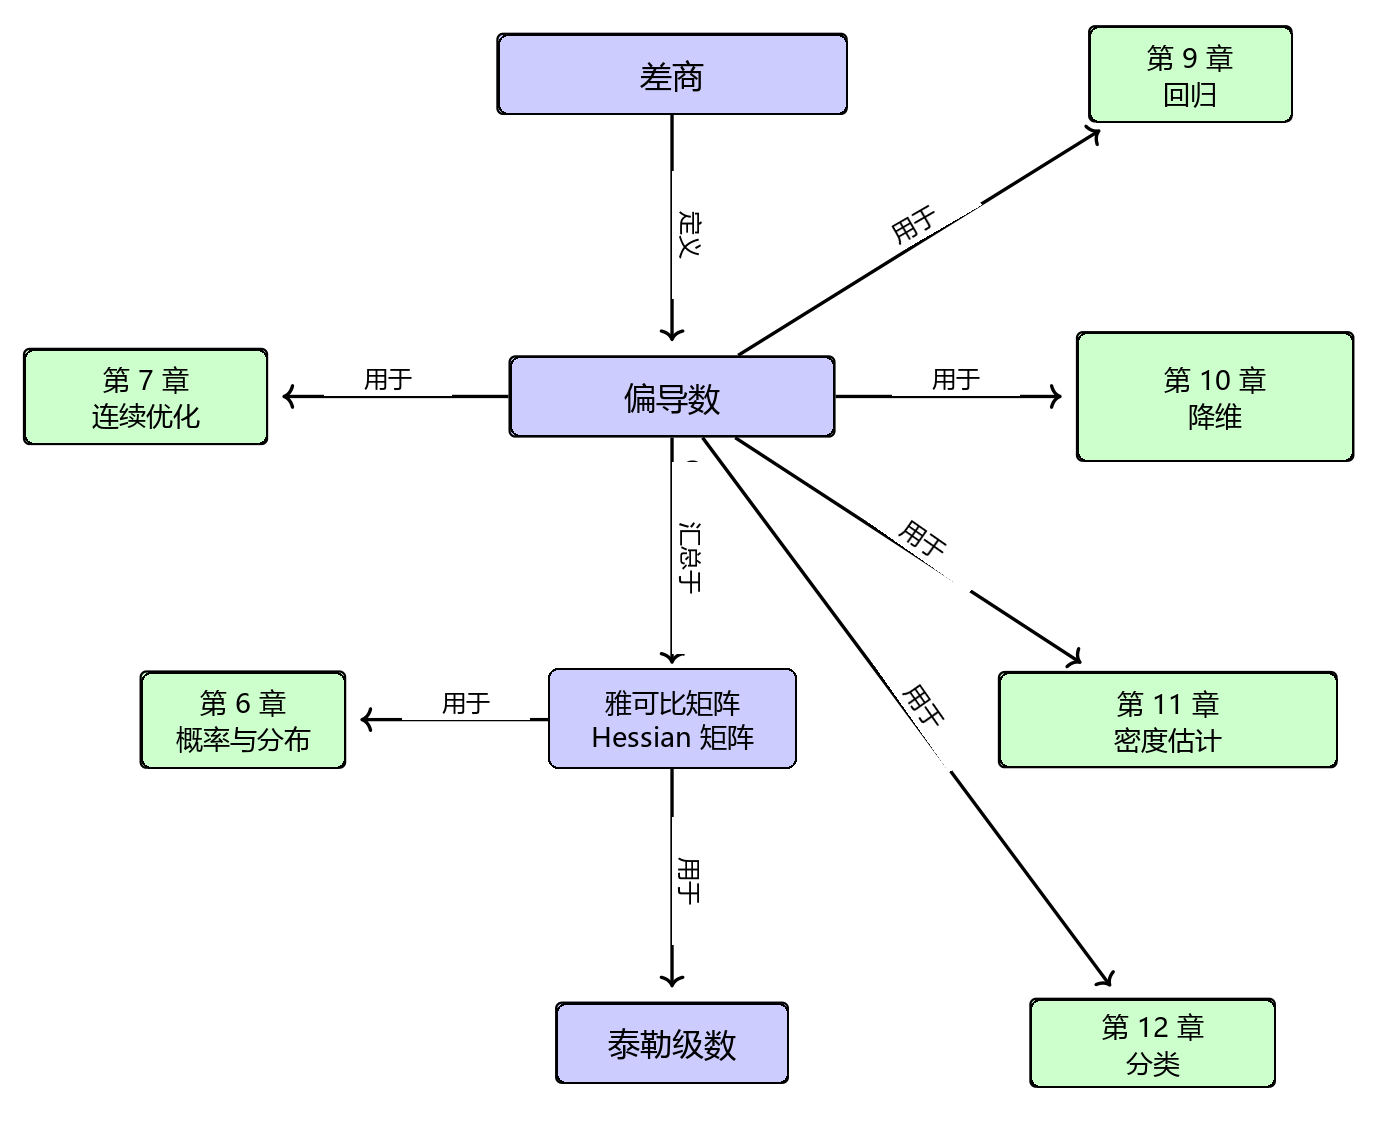
\includegraphics[width=0.92\textwidth,keepaspectratio]{docs/images/Figure5.2.png}
\caption*{\refstepcounter{figcounter}\label{fig:5-2}图~\thefigcounter 本章介绍的概念的思维导图，以及它们在本书其他部分中的应用场景。}
\end{figure}


在本章中，我们将讨论如何计算函数的梯度。梯度计算对于促进机器学习模型的学习通常是不可或缺的，因为梯度指向函数最陡上升的方向。因此，向量微积分是我们在机器学习中需要的基础数学工具之一。在本书通篇中，我们假设函数是可微的。借助一些额外的技术性定义（此处不予展开），所介绍的许多方法都可以扩展到次微分（在某些点连续但不可微的函数）。我们将在第 7 章中探讨对带约束函数情形的拓展。

\section*{5.1 单变量函数微分}
\addcontentsline{toc}{section}{5.1 单变量函数微分}
\label{sec:5.1}

下面，我们简要回顾单变量函数的微分，这在高中数学中可能已经很熟悉。我们首先从单变量函数 $ y = f(x) $（$ x, y \in \mathbb{R} $）的差商出发，随后利用它来定义导数。

\textbf{定义 5.1}（差商）。 \emph{差商（difference quotient）} ：

\begin{equation}
\frac{\delta y}{\delta x} := \frac{f(x + \delta x) - f(x)}{\delta x}
\tag{5.3}\label{eq:5-3}
\end{equation}

用于计算经过函数 $ f $ 图形上两点的割线斜率。在图~\ref{fig:5-3} 中，这两个点的 $ x $ 坐标分别为 $ x_0 $ 和 $ x_0 + \delta x $。


\begin{figure}[H]
\centering
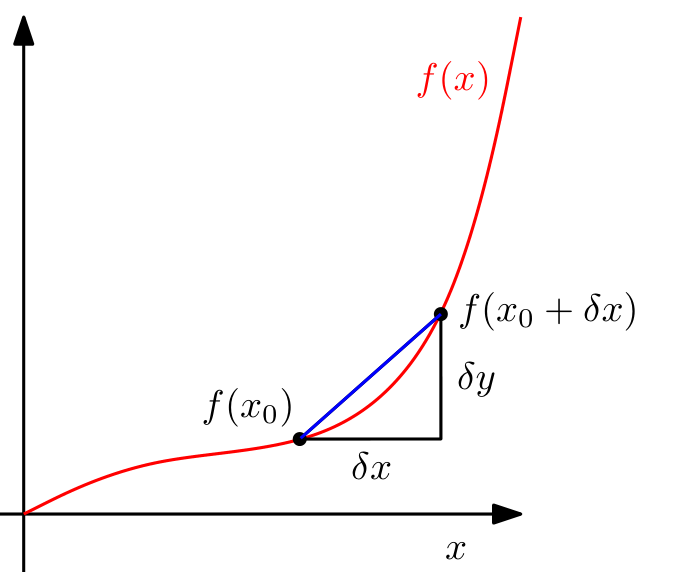
\includegraphics[width=0.92\textwidth,keepaspectratio]{docs/images/Figure5.3.png}
\caption*{\refstepcounter{figcounter}\label{fig:5-3}图~\thefigcounter 函数 f 在 x₀ 与 x₀ + δx 之间的平均倾斜度是通过 f(x₀) 和 f(x₀ + δx) 的割线（蓝色）的斜率，由 δy/δx 给出。}
\end{figure}


如果假定 $ f $ 为线性函数，差商也可以看作是 $ f $ 在 $ x $ 与 $ x + \delta x $ 之间的平均斜率。当 $ \delta x \to 0 $ 时，若 $ f $ 可微，极限即为 $ f $ 在 $ x $ 处的切线斜率。该切线即为 $ f $ 在 $ x $ 处的导数。

\textbf{定义 5.2}（导数）。更正式地，对于 $ h > 0 $，函数 $ f $ 在 $ x $ 处的 \emph{导数（derivative）} 定义为极限：

\begin{equation}
\frac{\mathrm{d}f}{\mathrm{d}x} := \lim_{h \to 0} \frac{f(x + h) - f(x)}{h}
\tag{5.4}\label{eq:5-4}
\end{equation}

此时图~\ref{fig:5-3} 中的割线收敛为切线。函数 $ f $ 的导数指向 $ f $ 最陡上升的方向。

\begin{notebox}
\textbf{例 5.2（多项式的导数）}
\end{notebox}

\begin{notebox}
我们希望计算 $ f(x) = x^n $（$ n \in \mathbb{N} $）的导数。我们可能已经知道结果是 $ n x^{n-1} $，但我们希望利用导数作为差商极限的定义来推导这一结果。
\end{notebox}

\begin{notebox}
利用式~\eqref{eq:5-4} 中导数的定义，我们有：

\begin{equation}
\frac{\mathrm{d}f}{\mathrm{d}x} = \lim_{h \to 0} \frac{f(x + h) - f(x)}{h}
\tag{5.5a}\label{eq:5-5a}
\end{equation}

\begin{equation}
= \lim_{h \to 0} \frac{(x + h)^n - x^n}{h}
\tag{5.5b}\label{eq:5-5b}
\end{equation}

\begin{equation}
= \lim_{h \to 0} \frac{\sum_{i=0}^n \binom{n}{i} x^{n-i} h^i - x^n}{h}
\tag{5.5c}\label{eq:5-5c}
\end{equation}

注意到 $ x^n = \binom{n}{0} x^{n-0} h^0 $。通过从 $ i = 1 $ 开始求和，常数项 $ x^n $ 相互抵消，从而得到：

\begin{equation}
\frac{\mathrm{d}f}{\mathrm{d}x} = \lim_{h \to 0} \frac{\sum_{i=1}^n \binom{n}{i} x^{n-i} h^i}{h}
\tag{5.6a}\label{eq:5-6a}
\end{equation}

\begin{equation}
= \lim_{h \to 0} \sum_{i=1}^n \binom{n}{i} x^{n-i} h^{i-1}
\tag{5.6b}\label{eq:5-6b}
\end{equation}

\begin{equation}
= \lim_{h \to 0} \left[ \binom{n}{1} x^{n-1} + \sum_{i=2}^n \binom{n}{i} x^{n-i} h^{i-1} \right]
\tag{5.6c}\label{eq:5-6c}
\end{equation}

在式~\eqref{eq:5-6c} 中，当 $ h \to 0 $ 时第二项趋向于 0，因此：

\begin{equation}
\frac{\mathrm{d}f}{\mathrm{d}x} = \frac{n!}{1!(n - 1)!} x^{n-1} = n x^{n-1}
\tag{5.6d}\label{eq:5-6d}
\end{equation}
\end{notebox}

\medskip\hrule\medskip

\section*{5.1.1 泰勒级数}
\addcontentsline{toc}{subsection}{5.1.1 泰勒级数}

泰勒级数是将函数 $ f $ 表示为无限项之和的一种形式。这些项由在 $ x_0 $ 处求值的 $ f $ 的各阶导数所决定。

\textbf{定义 5.3}（泰勒多项式）。函数 $ f : \mathbb{R} \to \mathbb{R} $ 在 $ x_0 $ 处的 $ n $ 阶 \emph{泰勒多项式（Taylor polynomial）} 定义为：

\begin{equation}
T_n(x) := \sum_{k=0}^n \frac{f^{(k)}(x_0)}{k!} (x - x_0)^k
\tag{5.7}\label{eq:5-7}
\end{equation}

其中 $ f^{(k)}(x_0) $ 是 $ f $ 在 $ x_0 $ 处的 $ k $ 阶导数（假定其存在），而 $ \frac{f^{(k)}(x_0)}{k!} $ 是多项式的系数。我们对所有 $ t \in \mathbb{R} $ 约定 $ t^0 := 1 $。

\textbf{定义 5.4}（泰勒级数）。对于光滑函数 $ f \in C^\infty $（$ f : \mathbb{R} \to \mathbb{R} $），$ f $ 在 $ x_0 $ 处的 \emph{泰勒级数（Taylor series）} 定义为：

\begin{equation}
T_\infty(x) = \sum_{k=0}^\infty \frac{f^{(k)}(x_0)}{k!} (x - x_0)^k
\tag{5.8}\label{eq:5-8}
\end{equation}

当 $ x_0 = 0 $ 时，我们获得作为泰勒级数特例的 \emph{麦克劳林级数（Maclaurin series）} 。如果 $ f(x) = T_\infty(x) $，则称 $ f $ 是 \emph{解析的（analytic）} 。这里 $ f \in C^\infty $ 表示 $ f $ 是无穷次连续可微的。

\emph{备注} 。一般而言，$ n $ 阶泰勒多项式是对函数的逼近，该函数本身不一定是多项式。泰勒多项式在 $ x_0 $ 的邻域内与 $ f $ 相似。然而，对于次数 $ k \leqslant n $ 的多项式 $ f $，$ n $ 阶泰勒多项式是该多项式的精确表示，因为所有阶数 $ i > k $ 的导数 $ f^{(i)} $ 全为 0。♦

\begin{notebox}
\textbf{例 5.3（泰勒多项式）}
\end{notebox}

\begin{notebox}
考虑多项式：

\begin{equation}
f(x) = x^4
\tag{5.9}\label{eq:5-9}
\end{equation}

我们求在 $ x_0 = 1 $ 处求值的泰勒多项式 $ T_6 $。首先计算各阶导数系数 $ f^{(k)}(1) $（$ k = 0, \ldots, 6 $）：

\begin{equation}
f(1) = 1
\tag{5.10}\label{eq:5-10}
\end{equation}

\begin{equation}
f'(1) = 4
\tag{5.11}\label{eq:5-11}
\end{equation}

\begin{equation}
f''(1) = 12
\tag{5.12}\label{eq:5-12}
\end{equation}

\begin{equation}
f^{(3)}(1) = 24
\tag{5.13}\label{eq:5-13}
\end{equation}

\begin{equation}
f^{(4)}(1) = 24
\tag{5.14}\label{eq:5-14}
\end{equation}

\begin{equation}
f^{(5)}(1) = 0
\tag{5.15}\label{eq:5-15}
\end{equation}

\begin{equation}
f^{(6)}(1) = 0
\tag{5.16}\label{eq:5-16}
\end{equation}

因此，所需的泰勒多项式为：

\begin{equation}
T_6(x) = \sum_{k=0}^6 \frac{f^{(k)}(x_0)}{k!} (x - x_0)^k
\tag{5.17a}\label{eq:5-17a}
\end{equation}

\begin{equation}
= 1 + 4(x - 1) + 6(x - 1)^2 + 4(x - 1)^3 + (x - 1)^4 + 0
\tag{5.17b}\label{eq:5-17b}
\end{equation}

展开并整理各项得到：

\begin{equation}
T_6(x) = (1 - 4 + 6 - 4 + 1) + x(4 - 12 + 12 - 4) + x^2(6 - 12 + 6) + x^3(4 - 4) + x^4
\tag{5.18a}\label{eq:5-18a}
\end{equation}

\begin{equation}
= x^4 = f(x)
\tag{5.18b}\label{eq:5-18b}
\end{equation}

即我们得到了原函数的精确表示。
\end{notebox}


\begin{figure}[H]
\centering
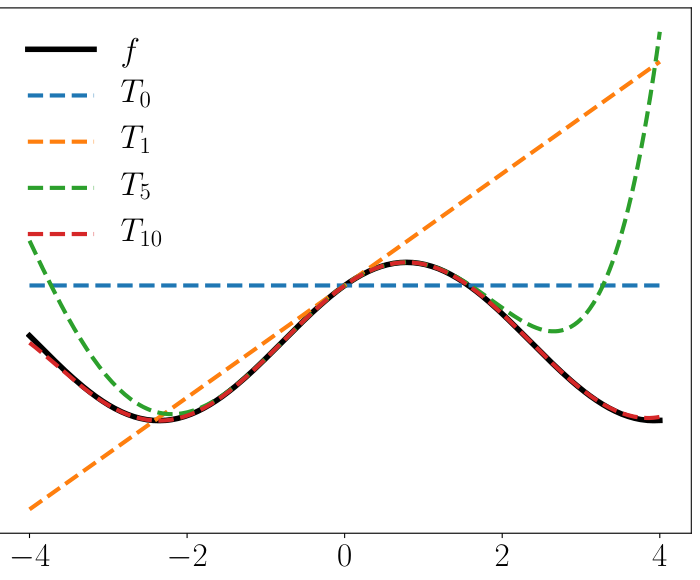
\includegraphics[width=0.92\textwidth,keepaspectratio]{docs/images/Figure5.4.png}
\caption*{\refstepcounter{figcounter}\label{fig:5-4}图~\thefigcounter 泰勒多项式。原函数 f(x) = sin(x) + cos(x)（黑色实线）在 x₀ = 0 处由各阶泰勒多项式（虚线）逼近。高阶泰勒多项式能更好地在更大全局范围内逼近函数 f。T₁₀ 在 [-4, 4] 区间内已经与 f 高度吻合。}
\end{figure}


\begin{notebox}
\textbf{例 5.4（泰勒级数）}
\end{notebox}

\begin{notebox}
考虑图~\ref{fig:5-4} 中给出的函数：

\begin{equation}
f(x) = \sin(x) + \cos(x) \in C^\infty
\tag{5.19}\label{eq:5-19}
\end{equation}

我们求 $ f $ 在 $ x_0 = 0 $ 处的泰勒级数展开（即麦克劳林级数展开）。我们得到以下导数：

\begin{equation}
f(0) = \sin(0) + \cos(0) = 1
\tag{5.20}\label{eq:5-20}
\end{equation}

\begin{equation}
f'(0) = \cos(0) - \sin(0) = 1
\tag{5.21}\label{eq:5-21}
\end{equation}

\begin{equation}
f''(0) = -\sin(0) - \cos(0) = -1
\tag{5.22}\label{eq:5-22}
\end{equation}

\begin{equation}
f^{(3)}(0) = -\cos(0) + \sin(0) = -1
\tag{5.23}\label{eq:5-23}
\end{equation}

\begin{equation}
f^{(4)}(0) = \sin(0) + \cos(0) = f(0) = 1
\tag{5.24}\label{eq:5-24}
\end{equation}

此处存在规律：泰勒级数中的系数仅为 $ \pm 1 $（因为 $ \sin(0) = 0 $），每两个相同符号后切换到另一个符号。此外，$ f^{(k+4)}(0) = f^{(k)}(0) $。
\end{notebox}

\begin{notebox}
因此，$ f $ 在 $ x_0 = 0 $ 处的完整泰勒级数展开为：

\begin{equation}
T_\infty(x) = \sum_{k=0}^\infty \frac{f^{(k)}(x_0)}{k!} (x - x_0)^k
\tag{5.25a}\label{eq:5-25a}
\end{equation}

\begin{equation}
= 1 + x - \frac{1}{2!} x^2 - \frac{1}{3!} x^3 + \frac{1}{4!} x^4 + \frac{1}{5!} x^5 - \cdots
\tag{5.25b}\label{eq:5-25b}
\end{equation}

\begin{equation}
= \left( 1 - \frac{1}{2!} x^2 + \frac{1}{4!} x^4 \mp \cdots \right) + \left( x - \frac{1}{3!} x^3 + \frac{1}{5!} x^5 \mp \cdots \right)
\tag{5.25c}\label{eq:5-25c}
\end{equation}

\begin{equation}
= \sum_{k=0}^\infty \frac{(-1)^k}{(2k)!} x^{2k} + \sum_{k=0}^\infty \frac{(-1)^k}{(2k + 1)!} x^{2k+1}
\tag{5.25d}\label{eq:5-25d}
\end{equation}

\begin{equation}
= \cos(x) + \sin(x)
\tag{5.25e}\label{eq:5-25e}
\end{equation}

其中我们使用了三角函数的幂级数表示：

\begin{equation}
\cos(x) = \sum_{k=0}^\infty \frac{(-1)^k}{(2k)!} x^{2k}
\tag{5.26}\label{eq:5-26}
\end{equation}

\begin{equation}
\sin(x) = \sum_{k=0}^\infty \frac{(-1)^k}{(2k + 1)!} x^{2k+1}
\tag{5.27}\label{eq:5-27}
\end{equation}

图~\ref{fig:5-4} 展示了 $ n = 0, 1, 5, 10 $ 时对应的泰勒多项式 $ T_n $。
\end{notebox}

\emph{备注} 。泰勒级数是 \emph{幂级数（power series）} ：

\begin{equation}
f(x) = \sum_{k=0}^\infty a_k (x - c)^k
\tag{5.28}\label{eq:5-28}
\end{equation}

的特例，其中 $ a_k $ 为系数，$ c $ 为常数，在定义 5.4 中具有特定的求值形式。♦

\medskip\hrule\medskip

\section*{5.1.2 微分法则}
\addcontentsline{toc}{subsection}{5.1.2 微分法则}

下面我们简要列出基本的微分法则，其中我们将 $ f $ 的导数记为 $ f' $：

\begin{itemize}
\item 乘积法则（Product rule）：
\end{itemize}

\begin{equation}
(f(x)g(x))' = f'(x)g(x) + f(x)g'(x)
\tag{5.29}\label{eq:5-29}
\end{equation}

\begin{itemize}
\item 商法则（Quotient rule）：
\end{itemize}

\begin{equation}
\left( \frac{f(x)}{g(x)} \right)' = \frac{f'(x)g(x) - f(x)g'(x)}{(g(x))^2}
\tag{5.30}\label{eq:5-30}
\end{equation}

\begin{itemize}
\item 求和法则（Sum rule）：
\end{itemize}

\begin{equation}
(f(x) + g(x))' = f'(x) + g'(x)
\tag{5.31}\label{eq:5-31}
\end{equation}

\begin{itemize}
\item 链式法则（Chain rule）：
\end{itemize}

\begin{equation}
(g(f(x)))' = (g \circ f)'(x) = g'(f(x))f'(x)
\tag{5.32}\label{eq:5-32}
\end{equation}

这里 $ g \circ f $ 表示复合函数 $ x \mapsto f(x) \mapsto g(f(x)) $。

\begin{notebox}
\textbf{例 5.5（链式法则）}
\end{notebox}

\begin{notebox}
我们使用链式法则计算函数 $ h(x) = (2x + 1)^4 $ 的导数。令：

\begin{equation}
h(x) = (2x + 1)^4 = g(f(x))
\tag{5.33}\label{eq:5-33}
\end{equation}

\begin{equation}
f(x) = 2x + 1
\tag{5.34}\label{eq:5-34}
\end{equation}

\begin{equation}
g(f) = f^4
\tag{5.35}\label{eq:5-35}
\end{equation}

我们得到 $ f $ 和 $ g $ 的导数分别为：

\begin{equation}
f'(x) = 2
\tag{5.36}\label{eq:5-36}
\end{equation}

\begin{equation}
g'(f) = 4f^3
\tag{5.37}\label{eq:5-37}
\end{equation}

从而 $ h $ 的导数为：

\begin{equation}
h'(x) = g'(f)f'(x) = (4f^3) \cdot 2 = 4(2x + 1)^3 \cdot 2 = 8(2x + 1)^3
\tag{5.38}\label{eq:5-38}
\end{equation}

其中我们应用了链式法则 (5.32)，并将式~\eqref{eq:5-34} 中 $ f $ 的定义代入了 $ g'(f) $。
\end{notebox}

\section*{5.2 偏微分与梯度}
\addcontentsline{toc}{section}{5.2 偏微分与梯度}
\label{sec:5.2}

第 5.1 节讨论的微分适用于标量变量 $ x \in \mathbb{R} $ 的函数 $ f $。下面，我们考虑更一般的情形，其中函数 $ f $ 依赖于一个或多个变量 $ \boldsymbol{x} \in \mathbb{R}^n $，例如 $ f(\boldsymbol{x}) = f(x_1, x_2) $。将导数推广到多元函数即为梯度。

我们通过每次改变一个变量并保持其他变量不变来求解函数 $ f $ 关于 $ \boldsymbol{x} $ 的梯度。此时梯度就是这些偏导数的集合。

\textbf{定义 5.5}（偏导数）。对于 $ n $ 个变量 $ x_1, \ldots, x_n $ 的函数 $ f : \mathbb{R}^n \to \mathbb{R} $，$ \boldsymbol{x} \mapsto f(\boldsymbol{x}) $（$ \boldsymbol{x} \in \mathbb{R}^n $），我们将其 \emph{偏导数（partial derivative）} 定义为：

\begin{equation}
\begin{adjustbox}{max width=\linewidth}
\begin{aligned}
\frac{\partial f}{\partial x_1} &= \lim_{h \to 0} \frac{f(x_1 + h, x_2, \ldots, x_n) - f(\boldsymbol{x})}{h} \\
&\ \ \vdots \\
\frac{\partial f}{\partial x_n} &= \lim_{h \to 0} \frac{f(x_1, \ldots, x_{n-1}, x_n + h) - f(\boldsymbol{x})}{h}
\end{aligned}
\end{adjustbox}
\tag{5.39}\label{eq:5-39}
\end{equation}

并将它们汇集在行向量中：

\begin{equation}
\begin{adjustbox}{max width=\linewidth}
\nabla_{\boldsymbol{x}} f = \mathrm{grad}\, f = \frac{\mathrm{d}f}{\mathrm{d}\boldsymbol{x}} = \begin{bmatrix} \frac{\partial f(\boldsymbol{x})}{\partial x_1} & \frac{\partial f(\boldsymbol{x})}{\partial x_2} & \cdots & \frac{\partial f(\boldsymbol{x})}{\partial x_n} \end{bmatrix} \in \mathbb{R}^{1 \times n}
\end{adjustbox}
\tag{5.40}\label{eq:5-40}
\end{equation}

其中 $ n $ 是变量的个数，而 $ 1 $ 是 $ f $ 的像/值域/到达域（image/range/codomain）的维度。这里，我们将列向量定义为 $ \boldsymbol{x} = [x_1, \ldots, x_n]^\top \in \mathbb{R}^n $。式~\eqref{eq:5-40} 中的行向量被称为 $ f $ 的 \emph{梯度（gradient）} 或 \emph{雅可比矩阵（Jacobian）} ，它是第 5.1 节中导数的推广。

\emph{备注} 。雅可比矩阵的这一定义是向量值函数雅可比矩阵（作为偏导数集合）一般定义的特例。我们将在第 5.3 节回到这一点。（ \emph{边注} ：我们可以利用标量微分的结果：每个偏导数都是关于一个标量的导数。）♦

\begin{notebox}
\textbf{例 5.6（利用链式法则求偏导数）}
\end{notebox}

\begin{notebox}
对于 $ f(x, y) = (x + 2y^3)^2 $，我们得到偏导数：

\begin{equation}
\frac{\partial f(x, y)}{\partial x} = 2(x + 2y^3) \frac{\partial}{\partial x}(x + 2y^3) = 2(x + 2y^3)
\tag{5.41}\label{eq:5-41}
\end{equation}

\begin{equation}
\frac{\partial f(x, y)}{\partial y} = 2(x + 2y^3) \frac{\partial}{\partial y}(x + 2y^3) = 12(x + 2y^3)y^2
\tag{5.42}\label{eq:5-42}
\end{equation}

其中我们利用了链式法则 (5.32) 来计算偏导数。
\end{notebox}

\emph{备注（作为行向量的梯度）} 。在文献中，将梯度向量定义为列向量的做法并不少见，这遵循了向量通常是列向量的惯例。我们将梯度向量定义为行向量的原因有两点：首先，我们可以一致地将梯度推广到向量值函数 $ \boldsymbol{f} : \mathbb{R}^n \to \mathbb{R}^m $（此时梯度成为一个矩阵）。其次，我们可以直接应用多元链式法则，而无需关注梯度的维度。我们将在第 5.3 节讨论这两点。♦

\begin{notebox}
\textbf{例 5.7（梯度）}
\end{notebox}

\begin{notebox}
对于 $ f(x_1, x_2) = x_1^2 x_2 + x_1 x_2^3 \in \mathbb{R} $，偏导数（即 $ f $ 关于 $ x_1 $ 和 $ x_2 $ 的导数）为：

\begin{equation}
\frac{\partial f(x_1, x_2)}{\partial x_1} = 2x_1 x_2 + x_2^3
\tag{5.43}\label{eq:5-43}
\end{equation}

\begin{equation}
\frac{\partial f(x_1, x_2)}{\partial x_2} = x_1^2 + 3x_1 x_2^2
\tag{5.44}\label{eq:5-44}
\end{equation}

相应的梯度为：

\begin{equation}
\begin{adjustbox}{max width=\linewidth}
\frac{\mathrm{d}f}{\mathrm{d}\boldsymbol{x}} = \begin{bmatrix} \frac{\partial f(x_1, x_2)}{\partial x_1} & \frac{\partial f(x_1, x_2)}{\partial x_2} \end{bmatrix} = \begin{bmatrix} 2x_1 x_2 + x_2^3 & x_1^2 + 3x_1 x_2^2 \end{bmatrix} \in \mathbb{R}^{1 \times 2}
\end{adjustbox}
\tag{5.45}\label{eq:5-45}
\end{equation}
\end{notebox}

\medskip\hrule\medskip

\section*{5.2.1 偏微分的基本法则}
\addcontentsline{toc}{subsection}{5.2.1 偏微分的基本法则}

在多元情形下（其中 $ \boldsymbol{x} \in \mathbb{R}^n $），我们在中学学到的基本微分法则（例如求和法则、乘积法则、链式法则；参见第 5.1.2 节）仍然适用。然而，当我们计算关于向量 $ \boldsymbol{x} \in \mathbb{R}^n $ 的导数时需要注意：此时我们的梯度涉及向量和矩阵，而矩阵乘法并不满足交换律（第 2.2.1 节），即相乘的顺序至关重要。

以下是一般的乘积法则、求和法则和链式法则：

\begin{itemize}
\item 乘积法则（Product rule）：
\end{itemize}

\begin{equation}
\frac{\partial}{\partial \boldsymbol{x}}(f(\boldsymbol{x})g(\boldsymbol{x})) = \frac{\partial f}{\partial \boldsymbol{x}} g(\boldsymbol{x}) + f(\boldsymbol{x})\frac{\partial g}{\partial \boldsymbol{x}}
\tag{5.46}\label{eq:5-46}
\end{equation}

\begin{itemize}
\item 求和法则（Sum rule）：
\end{itemize}

\begin{equation}
\frac{\partial}{\partial \boldsymbol{x}}(f(\boldsymbol{x}) + g(\boldsymbol{x})) = \frac{\partial f}{\partial \boldsymbol{x}} + \frac{\partial g}{\partial \boldsymbol{x}}
\tag{5.47}\label{eq:5-47}
\end{equation}

\begin{itemize}
\item 链式法则（Chain rule）：
\end{itemize}

\begin{equation}
\frac{\partial}{\partial \boldsymbol{x}}(g \circ f)(\boldsymbol{x}) = \frac{\partial}{\partial \boldsymbol{x}}(g(f(\boldsymbol{x}))) = \frac{\partial g}{\partial f} \frac{\partial f}{\partial \boldsymbol{x}}
\tag{5.48}\label{eq:5-48}
\end{equation}

让我们更仔细地审视链式法则。式~\eqref{eq:5-48} 的链式法则在某种程度上类似于矩阵乘法法则——我们在第 2.2.1 节中指出，相邻的维度必须匹配才能定义矩阵乘法。如果从左向右看，链式法则展现出类似的性质：$ \partial f $ 出现在第一个因子的“分母”和第二个因子的“分子”中。如果将这两个因子相乘，乘法是有定义的，即 $ \partial f $ 的维度匹配，且 $ \partial f $ 被“约去”，从而保留下 $ \partial g / \partial \boldsymbol{x} $。（ \emph{边注} ：这只是一种直观理解，在数学上并不严格，因为偏导数并不是分数。）

\medskip\hrule\medskip

\section*{5.2.2 链式法则}
\addcontentsline{toc}{subsection}{5.2.2 链式法则}

考虑关于两个变量 $ x_1, x_2 $ 的函数 $ f : \mathbb{R}^2 \to \mathbb{R} $。此外，$ x_1(t) $ 和 $ x_2(t) $ 本身是 $ t $ 的函数。为了计算 $ f $ 关于 $ t $ 的梯度，我们需要应用多元函数的链式法则 (5.48)：

\begin{equation}
\begin{adjustbox}{max width=\linewidth}
\frac{\mathrm{d}f}{\mathrm{d}t} = \begin{bmatrix} \frac{\partial f}{\partial x_1} & \frac{\partial f}{\partial x_2} \end{bmatrix} \begin{bmatrix} \frac{\partial x_1(t)}{\partial t} \\ \frac{\partial x_2(t)}{\partial t} \end{bmatrix} = \frac{\partial f}{\partial x_1}\frac{\partial x_1}{\partial t} + \frac{\partial f}{\partial x_2}\frac{\partial x_2}{\partial t}
\end{adjustbox}
\tag{5.49}\label{eq:5-49}
\end{equation}

其中 $ \mathrm{d} $ 表示梯度，而 $ \partial $ 表示偏导数。

\begin{notebox}
\textbf{例 5.8}
\end{notebox}

\begin{notebox}
考虑 $ f(x_1, x_2) = x_1^2 + 2x_2 $，其中 $ x_1 = \sin t $ 且 $ x_2 = \cos t $，则：

\begin{equation}
\frac{\mathrm{d}f}{\mathrm{d}t} = \frac{\partial f}{\partial x_1}\frac{\partial x_1}{\partial t} + \frac{\partial f}{\partial x_2}\frac{\partial x_2}{\partial t}
\tag{5.50a}\label{eq:5-50a}
\end{equation}

\begin{equation}
= 2 \sin t \frac{\partial \sin t}{\partial t} + 2 \frac{\partial \cos t}{\partial t}
\tag{5.50b}\label{eq:5-50b}
\end{equation}

\begin{equation}
= 2 \sin t \cos t - 2 \sin t = 2 \sin t(\cos t - 1)
\tag{5.50c}\label{eq:5-50c}
\end{equation}

即为 $ f $ 关于 $ t $ 的对应导数。
\end{notebox}

如果 $ f(x_1, x_2) $ 是 $ x_1 $ 和 $ x_2 $ 的函数，而 $ x_1(s, t) $ 和 $ x_2(s, t) $ 本身是两个变量 $ s $ 和 $ t $ 的函数，则链式法则给出偏导数：

\begin{equation}
\frac{\partial f}{\partial s} = \frac{\partial f}{\partial x_1}\frac{\partial x_1}{\partial s} + \frac{\partial f}{\partial x_2}\frac{\partial x_2}{\partial s}
\tag{5.51}\label{eq:5-51}
\end{equation}

\begin{equation}
\frac{\partial f}{\partial t} = \frac{\partial f}{\partial x_1}\frac{\partial x_1}{\partial t} + \frac{\partial f}{\partial x_2}\frac{\partial x_2}{\partial t}
\tag{5.52}\label{eq:5-52}
\end{equation}

相应的梯度可以通过矩阵乘法得到：

\begin{equation}
\begin{adjustbox}{max width=\linewidth}
\frac{\mathrm{d}f}{\mathrm{d}(s, t)} = \frac{\partial f}{\partial \boldsymbol{x}} \frac{\partial \boldsymbol{x}}{\partial(s, t)} = \underbrace{\begin{bmatrix} \frac{\partial f}{\partial x_1} & \frac{\partial f}{\partial x_2} \end{bmatrix}}_{= \frac{\partial f}{\partial \boldsymbol{x}}} \underbrace{\begin{bmatrix} \frac{\partial x_1}{\partial s} & \frac{\partial x_1}{\partial t} \\ \frac{\partial x_2}{\partial s} & \frac{\partial x_2}{\partial t} \end{bmatrix}}_{= \frac{\partial \boldsymbol{x}}{\partial(s, t)}}
\end{adjustbox}
\tag{5.53}\label{eq:5-53}
\end{equation}

将链式法则紧凑地写为矩阵乘法的这种形式，仅在梯度定义为行向量时才有意义。（ \emph{边注} ：链式法则可以写成矩阵乘法。）否则，我们将需要对梯度进行转置以使矩阵维度匹配。只要梯度是向量或矩阵，转置可能仍很简单；然而，当梯度变为张量时（我们将在后文中讨论），转置就不再是一件简单的事情了。

\emph{备注（验证梯度实现的正确性）} 。在计算机程序中数值检验梯度的正确性时，可以利用偏导数作为对应差商极限的定义（参见式~\eqref{eq:5-39}）：当我们计算梯度并实现它们时，我们可以使用有限差分在数值上测试我们的计算和实现——我们选取较小的 $ h $ 值（例如 $ h = 10^{-4} $），并将式~\eqref{eq:5-39} 中的有限差分逼近与梯度的（解析）实现进行比较。如果误差很小，我们的梯度实现很可能是正确的。“小”可以意味着：

\begin{equation*}
\sqrt{\frac{\sum_i (dh_i - df_i)^2}{\sum_i (dh_i + df_i)^2}} < 10^{-6}
\end{equation*}

其中 $ dh_i $ 是有限差分逼近，而 $ df_i $ 是 $ f $ 关于第 $ i $ 个变量 $ x_i $ 的解析梯度。这种方法被称为 \emph{梯度检验（gradient checking）} 。♦

\section*{5.3 向量值函数的梯度}
\addcontentsline{toc}{section}{5.3 向量值函数的梯度}
\label{sec:5.3}

到目前为止，我们讨论了映射到实数的函数 $ f : \mathbb{R}^n \to \mathbb{R} $ 的偏导数与梯度。下面，我们将梯度的概念推广到向量值函数（或称为 \emph{向量场（vector fields）} ）$ \boldsymbol{f} : \mathbb{R}^n \to \mathbb{R}^m $，其中 $ n \geqslant 1 $ 且 $ m > 1 $。

对于函数 $ \boldsymbol{f} : \mathbb{R}^n \to \mathbb{R}^m $ 和向量 $ \boldsymbol{x} = [x_1, \ldots, x_n]^\top \in \mathbb{R}^n $，对应的函数值向量由下式给出：

\begin{equation}
\boldsymbol{f}(\boldsymbol{x}) = \begin{bmatrix} f_1(\boldsymbol{x}) \\ \vdots \\ f_m(\boldsymbol{x}) \end{bmatrix} \in \mathbb{R}^m
\tag{5.54}\label{eq:5-54}
\end{equation}

将向量值函数写成这种形式，使我们能够将向量值函数 $ \boldsymbol{f} : \mathbb{R}^n \to \mathbb{R}^m $ 视为映射到 $ \mathbb{R} $ 的函数向量 $ [f_1, \ldots, f_m]^\top $（其中 $ f_i : \mathbb{R}^n \to \mathbb{R} $）。每个 $ f_i $ 的微分法则正是我们在第 5.2 节中讨论过的法则。

因此，向量值函数 $ \boldsymbol{f} : \mathbb{R}^n \to \mathbb{R}^m $ 关于 $ x_i \in \mathbb{R} $（$ i = 1, \ldots, n $）的偏导数由如下向量给出：

\begin{equation}
\begin{adjustbox}{max width=\linewidth}
\frac{\partial \boldsymbol{f}}{\partial x_i} = \begin{bmatrix} \frac{\partial f_1}{\partial x_i} \\ \vdots \\ \frac{\partial f_m}{\partial x_i} \end{bmatrix} = \begin{bmatrix} \lim_{h \to 0} \frac{f_1(x_1, \ldots, x_{i-1}, x_i + h, x_{i+1}, \ldots, x_n) - f_1(\boldsymbol{x})}{h} \\ \vdots \\ \lim_{h \to 0} \frac{f_m(x_1, \ldots, x_{i-1}, x_i + h, x_{i+1}, \ldots, x_n) - f_m(\boldsymbol{x})}{h} \end{bmatrix} \in \mathbb{R}^m
\end{adjustbox}
\tag{5.55}\label{eq:5-55}
\end{equation}

由式~\eqref{eq:5-40} 可知，$ f $ 关于一个向量的梯度是偏导数的行向量。在式~\eqref{eq:5-55} 中，每个偏导数 $ \partial \boldsymbol{f} / \partial x_i $ 都是一个列向量。因此，通过收集这些偏导数，我们得到 $ \boldsymbol{f} : \mathbb{R}^n \to \mathbb{R}^m $ 关于 $ \boldsymbol{x} \in \mathbb{R}^n $ 的梯度：

\begin{equation}
\begin{adjustbox}{max width=\linewidth}
\frac{\mathrm{d}\boldsymbol{f}(\boldsymbol{x})}{\mathrm{d}\boldsymbol{x}} = \begin{bmatrix} \frac{\partial \boldsymbol{f}(\boldsymbol{x})}{\partial x_1} & \cdots & \frac{\partial \boldsymbol{f}(\boldsymbol{x})}{\partial x_n} \end{bmatrix}
\end{adjustbox}
\tag{5.56a}\label{eq:5-56a}
\end{equation}

\begin{equation}
\begin{adjustbox}{max width=\linewidth}
= \begin{bmatrix} \frac{\partial f_1(\boldsymbol{x})}{\partial x_1} & \cdots & \frac{\partial f_1(\boldsymbol{x})}{\partial x_n} \\ \vdots & & \vdots \\ \frac{\partial f_m(\boldsymbol{x})}{\partial x_1} & \cdots & \frac{\partial f_m(\boldsymbol{x})}{\partial x_n} \end{bmatrix} \in \mathbb{R}^{m \times n}
\end{adjustbox}
\tag{5.56b}\label{eq:5-56b}
\end{equation}

\textbf{定义 5.6}（雅可比矩阵）。向量值函数 $ \boldsymbol{f} : \mathbb{R}^n \to \mathbb{R}^m $ 的所有一阶偏导数的集合称为 \emph{雅可比矩阵（Jacobian）} 。雅可比矩阵 $ \boldsymbol{J} $ 是一个 $ m \times n $ 矩阵，我们将其定义并排列如下（ \emph{边注} ：函数 $ \boldsymbol{f} : \mathbb{R}^n \to \mathbb{R}^m $ 的梯度是一个大小为 $ m \times n $ 的矩阵）：

\begin{equation}
\begin{adjustbox}{max width=\linewidth}
\boldsymbol{J} = \nabla_{\boldsymbol{x}} \boldsymbol{f} = \frac{\mathrm{d}\boldsymbol{f}(\boldsymbol{x})}{\mathrm{d}\boldsymbol{x}} = \begin{bmatrix} \frac{\partial \boldsymbol{f}(\boldsymbol{x})}{\partial x_1} & \cdots & \frac{\partial \boldsymbol{f}(\boldsymbol{x})}{\partial x_n} \end{bmatrix}
\end{adjustbox}
\tag{5.57}\label{eq:5-57}
\end{equation}

\begin{equation}
\begin{adjustbox}{max width=\linewidth}
= \begin{bmatrix} \frac{\partial f_1(\boldsymbol{x})}{\partial x_1} & \cdots & \frac{\partial f_1(\boldsymbol{x})}{\partial x_n} \\ \vdots & & \vdots \\ \frac{\partial f_m(\boldsymbol{x})}{\partial x_1} & \cdots & \frac{\partial f_m(\boldsymbol{x})}{\partial x_n} \end{bmatrix}
\end{adjustbox}
\tag{5.58}\label{eq:5-58}
\end{equation}

\begin{equation}
\boldsymbol{x} = \begin{bmatrix} x_1 \\ \vdots \\ x_n \end{bmatrix}, \quad \boldsymbol{J}(i, j) = \frac{\partial f_i}{\partial x_j}
\tag{5.59}\label{eq:5-59}
\end{equation}

作为式~\eqref{eq:5-58} 的特例，将向量 $ \boldsymbol{x} \in \mathbb{R}^n $ 映射到标量的函数 $ f : \mathbb{R}^n \to \mathbb{R}^1 $（例如 $ f(\boldsymbol{x}) = \sum_{i=1}^n x_i $）的雅可比矩阵是一个行向量（维度为 $ 1 \times n $ 的矩阵）；参见式~\eqref{eq:5-40}。

\emph{备注} 。在本书中，我们使用导数的 \emph{分子布局（numerator layout）} ，即 $ \boldsymbol{f} \in \mathbb{R}^m $ 关于 $ \boldsymbol{x} \in \mathbb{R}^n $ 的导数 $ \mathrm{d}\boldsymbol{f} / \mathrm{d}\boldsymbol{x} $ 是一个 $ m \times n $ 矩阵，其中 $ \boldsymbol{f} $ 的元素定义行，$ \boldsymbol{x} $ 的元素定义相应雅可比矩阵的列；参见式~\eqref{eq:5-58}。此外还存在 \emph{分母布局（denominator layout）} ，它是分子布局的转置。在本书中，我们将统一采用分子布局。♦

我们将在第 6.7 节看到如何将雅可比矩阵用于概率分布的变量替换法中。由变量变换导致的缩放程度由行列式给出。

在第 4.1 节中，我们看到行列式可用于计算平行四边形的面积。如果给定两个向量 $ \boldsymbol{b}_1 = [1, 0]^\top, \boldsymbol{b}_2 = [0, 1]^\top $ 作为单位正方形的边（图~\ref{fig:5-5} 中的蓝色区域），该正方形的面积为：

\begin{equation}
\left| \det \begin{bmatrix} 1 & 0 \\ 0 & 1 \end{bmatrix} \right| = 1
\tag{5.60}\label{eq:5-60}
\end{equation}

如果我们取边为 $ \boldsymbol{c}_1 = [-2, 1]^\top, \boldsymbol{c}_2 = [1, 1]^\top $ 的平行四边形（图~\ref{fig:5-5} 中的橙色区域），其面积由行列式的绝对值给出（参见第 4.1 节）：

\begin{equation}
\left| \det \begin{bmatrix} -2 & 1 \\ 1 & 1 \end{bmatrix} \right| = |-3| = 3
\tag{5.61}\label{eq:5-61}
\end{equation}

即该平行四边形的面积恰好是单位正方形面积的三倍。我们可以通过寻找将单位正方形变换为该平行四边形的映射来求出该缩放因子。用线性代数的语言来说，我们实际上执行了从 $ (\boldsymbol{b}_1, \boldsymbol{b}_2) $ 到 $ (\boldsymbol{c}_1, \boldsymbol{c}_2) $ 的变量变换。在我们的示例中，该映射是线性的，并且该映射的行列式绝对值恰好给出了我们所寻找的缩放因子。


\begin{figure}[H]
\centering
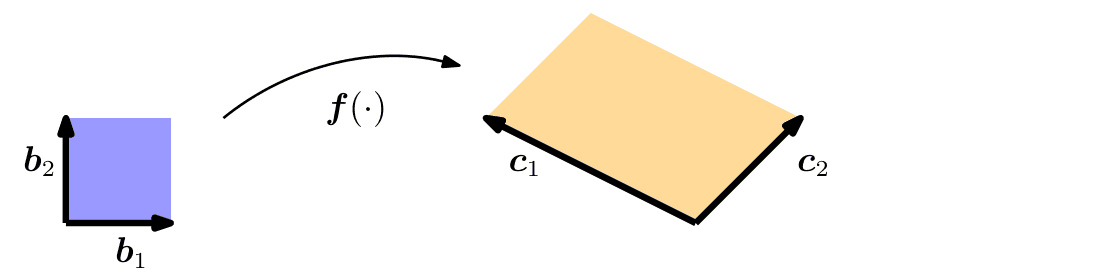
\includegraphics[width=0.92\textwidth,keepaspectratio]{docs/images/Figure5.5.png}
\caption*{\refstepcounter{figcounter}\label{fig:5-5}图~\thefigcounter f 的雅可比行列式可用于计算蓝色区域与橙色区域之间的放大倍数。}
\end{figure}


我们将介绍确定该映射的两种方法。首先，我们利用该映射是线性的这一事实，借助第 2 章中的工具来确定该映射。其次，我们将使用本章讨论的偏导数工具来寻找该映射。

\textbf{方法 1}。为了从线性代数方法入手，我们将 $ \{\boldsymbol{b}_1, \boldsymbol{b}_2\} $ 和 $ \{\boldsymbol{c}_1, \boldsymbol{c}_2\} $ 都视为 $ \mathbb{R}^2 $ 的基（参见第 2.6.1 节的回顾）。我们实际执行的是从 $ (\boldsymbol{b}_1, \boldsymbol{b}_2) $ 到 $ (\boldsymbol{c}_1, \boldsymbol{c}_2) $ 的基变换，并且正在寻找实现该基变换的变换矩阵。利用第 2.7.2 节的结果，我们将所需的基变换矩阵确定为：

\begin{equation}
\boldsymbol{J} = \begin{bmatrix} -2 & 1 \\ 1 & 1 \end{bmatrix}
\tag{5.62}\label{eq:5-62}
\end{equation}

使得 $ \boldsymbol{J} \boldsymbol{b}_1 = \boldsymbol{c}_1 $ 且 $ \boldsymbol{J} \boldsymbol{b}_2 = \boldsymbol{c}_2 $。给出我们所寻求的缩放因子的 $ \boldsymbol{J} $ 的行列式绝对值为 $ |\det(\boldsymbol{J})| = 3 $，即由 $ (\boldsymbol{c}_1, \boldsymbol{c}_2) $ 张成的面积是由 $ (\boldsymbol{b}_1, \boldsymbol{b}_2) $ 张成的面积的三倍。

\textbf{方法 2}。线性代数方法适用于线性变换；对于非线性变换（这在第 6.7 节中会变得很重要），我们采用基于偏导数的更通用方法。对于这种方法，我们考虑执行变量变换的函数 $ \boldsymbol{f} : \mathbb{R}^2 \to \mathbb{R}^2 $。在我们的示例中，$ \boldsymbol{f} $ 将任何向量 $ \boldsymbol{x} \in \mathbb{R}^2 $ 关于 $ (\boldsymbol{b}_1, \boldsymbol{b}_2) $ 的坐标表示映射到关于 $ (\boldsymbol{c}_1, \boldsymbol{c}_2) $ 的坐标表示 $ \boldsymbol{y} \in \mathbb{R}^2 $。我们希望确定该映射，以便计算当面积（或体积）被 $ \boldsymbol{f} $ 变换时是如何改变的。为此，我们需要弄清楚如果对 $ \boldsymbol{x} $ 进行微小修改，$ \boldsymbol{f}(\boldsymbol{x}) $ 会如何改变。这个问题正是由雅可比矩阵 $ \frac{\mathrm{d}\boldsymbol{f}}{\mathrm{d}\boldsymbol{x}} \in \mathbb{R}^{2 \times 2} $ 所回答的。因为我们可以写出：

\begin{equation}
y_1 = -2x_1 + x_2
\tag{5.63}\label{eq:5-63}
\end{equation}

\begin{equation}
y_2 = x_1 + x_2
\tag{5.64}\label{eq:5-64}
\end{equation}

从而获得了 $ \boldsymbol{x} $ 和 $ \boldsymbol{y} $ 之间的函数关系，由此可以求得偏导数：

\begin{equation}
\frac{\partial y_1}{\partial x_1} = -2, \quad \frac{\partial y_1}{\partial x_2} = 1, \quad \frac{\partial y_2}{\partial x_1} = 1, \quad \frac{\partial y_2}{\partial x_2} = 1
\tag{5.65}\label{eq:5-65}
\end{equation}

并构成雅可比矩阵：

\begin{equation}
\begin{adjustbox}{max width=\linewidth}
\boldsymbol{J} = \begin{bmatrix} \frac{\partial y_1}{\partial x_1} & \frac{\partial y_1}{\partial x_2} \\ \frac{\partial y_2}{\partial x_1} & \frac{\partial y_2}{\partial x_2} \end{bmatrix} = \begin{bmatrix} -2 & 1 \\ 1 & 1 \end{bmatrix}
\end{adjustbox}
\tag{5.66}\label{eq:5-66}
\end{equation}

该雅可比矩阵表示我们正在寻找的坐标变换。如果坐标变换是线性的（如我们的示例），该变换是精确的，且式~\eqref{eq:5-66} 精确地恢复了式~\eqref{eq:5-62} 中的基变换矩阵。如果坐标变换是非线性的，雅可比矩阵在局部用线性变换来逼近该非线性变换。 \emph{雅可比行列式（Jacobian determinant）} 的绝对值 $ |\det(\boldsymbol{J})| $ 是坐标变换时面积或体积缩放的因子。（ \emph{边注} ：从几何上看，当我们变换面积或体积时，雅可比行列式给出了放大/缩放因子。）在我们的示例中，$ |\det(\boldsymbol{J})| = 3 $。

雅可比行列式和变量变换在第 6.7 节变换随机变量和概率分布时将变得非常重要。在机器学习中，在使用 \emph{重参数化技巧（reparametrization trick）} （也称为 \emph{无穷小微扰分析（infinite perturbation analysis）} ）训练深度神经网络的背景下，这些变换极其重要。


\begin{figure}[H]
\centering
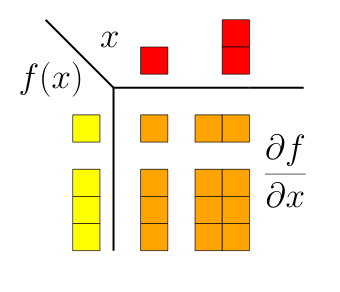
\includegraphics[width=0.92\textwidth,keepaspectratio]{docs/images/Figure5.6.png}
\caption*{\refstepcounter{figcounter}\label{fig:5-6}图~\thefigcounter （偏）导数的维度总结。}
\end{figure}


在本章中，我们遇到了各种函数的导数。图~\ref{fig:5-6} 总结了这些导数的维度。若 $ f : \mathbb{R} \to \mathbb{R} $，梯度就是一个标量（左上角）；对于 $ f : \mathbb{R}^D \to \mathbb{R} $，梯度是一个 $ 1 \times D $ 的行向量（右上角）；对于 $ \boldsymbol{f} : \mathbb{R} \to \mathbb{R}^E $，梯度是一个 $ E \times 1 $ 的列向量（左下角）；对于 $ \boldsymbol{f} : \mathbb{R}^D \to \mathbb{R}^E $，梯度是一个 $ E \times D $ 的矩阵（右下角）。

\begin{notebox}
\textbf{例 5.9（向量值函数的梯度）}
\end{notebox}

\begin{notebox}
设给定：

\begin{equation*}
\boldsymbol{f}(\boldsymbol{x}) = \boldsymbol{A} \boldsymbol{x}, \quad \boldsymbol{f}(\boldsymbol{x}) \in \mathbb{R}^M, \quad \boldsymbol{A} \in \mathbb{R}^{M \times N}, \quad \boldsymbol{x} \in \mathbb{R}^N
\end{equation*}

为了计算梯度 $ \mathrm{d}\boldsymbol{f} / \mathrm{d}\boldsymbol{x} $，首先确定 $ \mathrm{d}\boldsymbol{f} / \mathrm{d}\boldsymbol{x} $ 的维度：由于 $ \boldsymbol{f} : \mathbb{R}^N \to \mathbb{R}^M $，因此 $ \mathrm{d}\boldsymbol{f} / \mathrm{d}\boldsymbol{x} \in \mathbb{R}^{M \times N} $。其次，为了计算梯度，我们确定 $ \boldsymbol{f} $ 关于每个 $ x_j $ 的偏导数：

\begin{equation}
f_i(\boldsymbol{x}) = \sum_{j=1}^N A_{ij} x_j \implies \frac{\partial f_i}{\partial x_j} = A_{ij}
\tag{5.67}\label{eq:5-67}
\end{equation}

我们将这些偏导数汇集到雅可比矩阵中，从而得到梯度：

\begin{equation}
\begin{adjustbox}{max width=\linewidth}
\frac{\mathrm{d}\boldsymbol{f}}{\mathrm{d}\boldsymbol{x}} = \begin{bmatrix} \frac{\partial f_1}{\partial x_1} & \cdots & \frac{\partial f_1}{\partial x_N} \\ \vdots & & \vdots \\ \frac{\partial f_M}{\partial x_1} & \cdots & \frac{\partial f_M}{\partial x_N} \end{bmatrix} = \begin{bmatrix} A_{11} & \cdots & A_{1N} \\ \vdots & & \vdots \\ A_{M1} & \cdots & A_{MN} \end{bmatrix} = \boldsymbol{A} \in \mathbb{R}^{M \times N}
\end{adjustbox}
\tag{5.68}\label{eq:5-68}
\end{equation}
\end{notebox}

\begin{notebox}
\textbf{例 5.10（链式法则）}
\end{notebox}

\begin{notebox}
考虑函数 $ h : \mathbb{R} \to \mathbb{R} $，$ h(t) = (f \circ \boldsymbol{g})(t) $，其中：

\begin{equation}
f : \mathbb{R}^2 \to \mathbb{R}
\tag{5.69}\label{eq:5-69}
\end{equation}

\begin{equation}
\boldsymbol{g} : \mathbb{R} \to \mathbb{R}^2
\tag{5.70}\label{eq:5-70}
\end{equation}

\begin{equation}
f(\boldsymbol{x}) = \exp(x_1 x_2^2)
\tag{5.71}\label{eq:5-71}
\end{equation}

\begin{equation}
\boldsymbol{x} = \begin{bmatrix} x_1 \\ x_2 \end{bmatrix} = \boldsymbol{g}(t) = \begin{bmatrix} t \cos t \\ t \sin t \end{bmatrix}
\tag{5.72}\label{eq:5-72}
\end{equation}

我们计算 $ h $ 关于 $ t $ 的梯度。由于 $ f : \mathbb{R}^2 \to \mathbb{R} $ 且 $ \boldsymbol{g} : \mathbb{R} \to \mathbb{R}^2 $，我们注意到：

\begin{equation}
\frac{\partial f}{\partial \boldsymbol{x}} \in \mathbb{R}^{1 \times 2}, \quad \frac{\partial \boldsymbol{g}}{\partial t} \in \mathbb{R}^{2 \times 1}
\tag{5.73}\label{eq:5-73}
\end{equation}

所求梯度通过应用链式法则计算：

\begin{equation}
\begin{adjustbox}{max width=\linewidth}
\frac{\mathrm{d}h}{\mathrm{d}t} = \frac{\partial f}{\partial \boldsymbol{x}}\frac{\partial \boldsymbol{x}}{\partial t} = \begin{bmatrix} \frac{\partial f}{\partial x_1} & \frac{\partial f}{\partial x_2} \end{bmatrix} \begin{bmatrix} \frac{\partial x_1}{\partial t} \\ \frac{\partial x_2}{\partial t} \end{bmatrix}
\end{adjustbox}
\tag{5.74a}\label{eq:5-74a}
\end{equation}

\begin{equation}
= \begin{bmatrix} \exp(x_1 x_2^2) x_2^2 & 2\exp(x_1 x_2^2) x_1 x_2 \end{bmatrix} \begin{bmatrix} \cos t - t\sin t \\ \sin t + t\cos t \end{bmatrix}
\tag{5.74b}\label{eq:5-74b}
\end{equation}

\begin{equation}
= \exp(x_1 x_2^2) \left( x_2^2(\cos t - t\sin t) + 2x_1 x_2(\sin t + t\cos t) \right)
\tag{5.74c}\label{eq:5-74c}
\end{equation}

其中 $ x_1 = t \cos t $ 且 $ x_2 = t \sin t $；参见式~\eqref{eq:5-72}。
\end{notebox}

\begin{notebox}
\textbf{例 5.11（线性模型中最小二乘损失的梯度）}
\end{notebox}

\begin{notebox}
考虑线性模型：

\begin{equation}
\boldsymbol{y} = \boldsymbol{\Phi} \boldsymbol{\theta}
\tag{5.75}\label{eq:5-75}
\end{equation}

其中 $ \boldsymbol{\theta} \in \mathbb{R}^D $ 是参数向量，$ \boldsymbol{\Phi} \in \mathbb{R}^{N \times D} $ 是输入特征，而 $ \boldsymbol{y} \in \mathbb{R}^N $ 是对应的观测值。（ \emph{边注} ：我们将在第 9 章线性回归的背景下更详细地讨论该模型，在那里我们需要最小二乘损失 $ L $ 关于参数 $ \boldsymbol{\theta} $ 的导数。）我们定义函数：

\begin{equation}
L(\boldsymbol{e}) := \|\boldsymbol{e}\|^2
\tag{5.76}\label{eq:5-76}
\end{equation}

\begin{equation}
\boldsymbol{e}(\boldsymbol{\theta}) := \boldsymbol{y} - \boldsymbol{\Phi} \boldsymbol{\theta}
\tag{5.77}\label{eq:5-77}
\end{equation}

我们求解 $ \frac{\partial L}{\partial \boldsymbol{\theta}} $，并将为此应用链式法则。$ L $ 称为 \emph{最小二乘损失函数（least-squares loss function）} 。
\end{notebox}

\begin{notebox}
在开始计算之前，我们确定梯度的维度为：

\begin{equation}
\frac{\partial L}{\partial \boldsymbol{\theta}} \in \mathbb{R}^{1 \times D}
\tag{5.78}\label{eq:5-78}
\end{equation}

链式法则允许我们将梯度计算为：

\begin{equation}
\frac{\partial L}{\partial \boldsymbol{\theta}} = \frac{\partial L}{\partial \boldsymbol{e}} \frac{\partial \boldsymbol{e}}{\partial \boldsymbol{\theta}}
\tag{5.79}\label{eq:5-79}
\end{equation}

其中第 $ d $ 个元素由下式给出：

\begin{equation}
\frac{\partial L}{\partial \boldsymbol{\theta}}[1, d] = \sum_{n=1}^N \frac{\partial L}{\partial \boldsymbol{e}}[n] \frac{\partial \boldsymbol{e}}{\partial \boldsymbol{\theta}}[n, d]
\tag{5.80}\label{eq:5-80}
\end{equation}

（在 Python 中对应为 \texttt{dLdtheta = np.einsum('n,nd', dLde, dedtheta)}。） 我们知道 $ \|\boldsymbol{e}\|^2 = \boldsymbol{e}^\top \boldsymbol{e} $（参见第 3.2 节），由此确定：

\begin{equation}
\frac{\partial L}{\partial \boldsymbol{e}} = 2\boldsymbol{e}^\top \in \mathbb{R}^{1 \times N}
\tag{5.81}\label{eq:5-81}
\end{equation}

此外，我们得到：

\begin{equation}
\frac{\partial \boldsymbol{e}}{\partial \boldsymbol{\theta}} = -\boldsymbol{\Phi} \in \mathbb{R}^{N \times D}
\tag{5.82}\label{eq:5-82}
\end{equation}

从而所求的导数为：

\begin{equation}
\begin{adjustbox}{max width=\linewidth}
\frac{\partial L}{\partial \boldsymbol{\theta}} = -2\boldsymbol{e}^\top \boldsymbol{\Phi} \stackrel{(5.77)}{=} \underbrace{-2(\boldsymbol{y}^\top - \boldsymbol{\theta}^\top \boldsymbol{\Phi}^\top)}_{1 \times N} \underbrace{\boldsymbol{\Phi}}_{N \times D} \in \mathbb{R}^{1 \times D}
\end{adjustbox}
\tag{5.83}\label{eq:5-83}
\end{equation}
\end{notebox}

\emph{备注} 。如果不使用链式法则，而是直接考察函数：

\begin{equation}
L_2(\boldsymbol{\theta}) := \|\boldsymbol{y} - \boldsymbol{\Phi} \boldsymbol{\theta}\|^2 = (\boldsymbol{y} - \boldsymbol{\Phi} \boldsymbol{\theta})^\top (\boldsymbol{y} - \boldsymbol{\Phi} \boldsymbol{\theta})
\tag{5.84}\label{eq:5-84}
\end{equation}

我们也会得到相同的结果。对于像 $ L_2 $ 这样的简单函数，这种直接方法仍然是可行的，但对于深层复合函数而言，这种方法就变得不切实际了。♦

\section*{5.4 矩阵的梯度}
\addcontentsline{toc}{section}{5.4 矩阵的梯度}
\label{sec:5.4}

我们会遇到需要计算矩阵关于向量（或其他矩阵）的梯度的情形，这会导致产生多维 \emph{张量（tensor）} 。我们可以将这种张量视为收集偏导数的多维数组。（ \emph{边注} ：我们可以将张量视为多维数组。）例如，如果我们计算一个 $ m \times n $ 矩阵 $ \boldsymbol{A} $ 关于一个 $ p \times q $ 矩阵 $ \boldsymbol{B} $ 的梯度，所得的雅可比对象将是 $ (m \times n) \times (p \times q) $ 维的，即一个四维张量 $ \boldsymbol{J} $，其元素由 $ J_{ijkl} = \partial A_{ij} / \partial B_{kl} $ 给出。

由于矩阵表示线性映射，我们可以利用这样一个事实：$ m \times n $ 矩阵空间 $ \mathbb{R}^{m \times n} $ 与 $ mn $ 维向量空间 $ \mathbb{R}^{mn} $ 之间存在 \emph{向量空间同构（vector-space isomorphism）} （线性可逆映射）。因此，我们可以将矩阵分别重塑为长度为 $ mn $ 和 $ pq $ 的向量。使用这些向量进行求导将产生一个大小为 $ mn \times pq $ 的雅可比矩阵。图~\ref{fig:5-7} 对这两种方法进行了可视化展示。在实际应用中，通常更希望将矩阵重塑为向量并继续使用这个雅可比矩阵：（ \emph{边注} ：可以通过按列堆叠矩阵的元素将矩阵转换为向量，即“展平”。）链式法则 (5.48) 简化为普通的矩阵乘法，而对于雅可比张量的情形，我们将需要更多地注意对哪些维度进行求和消除。


\begin{figure}[H]
\centering
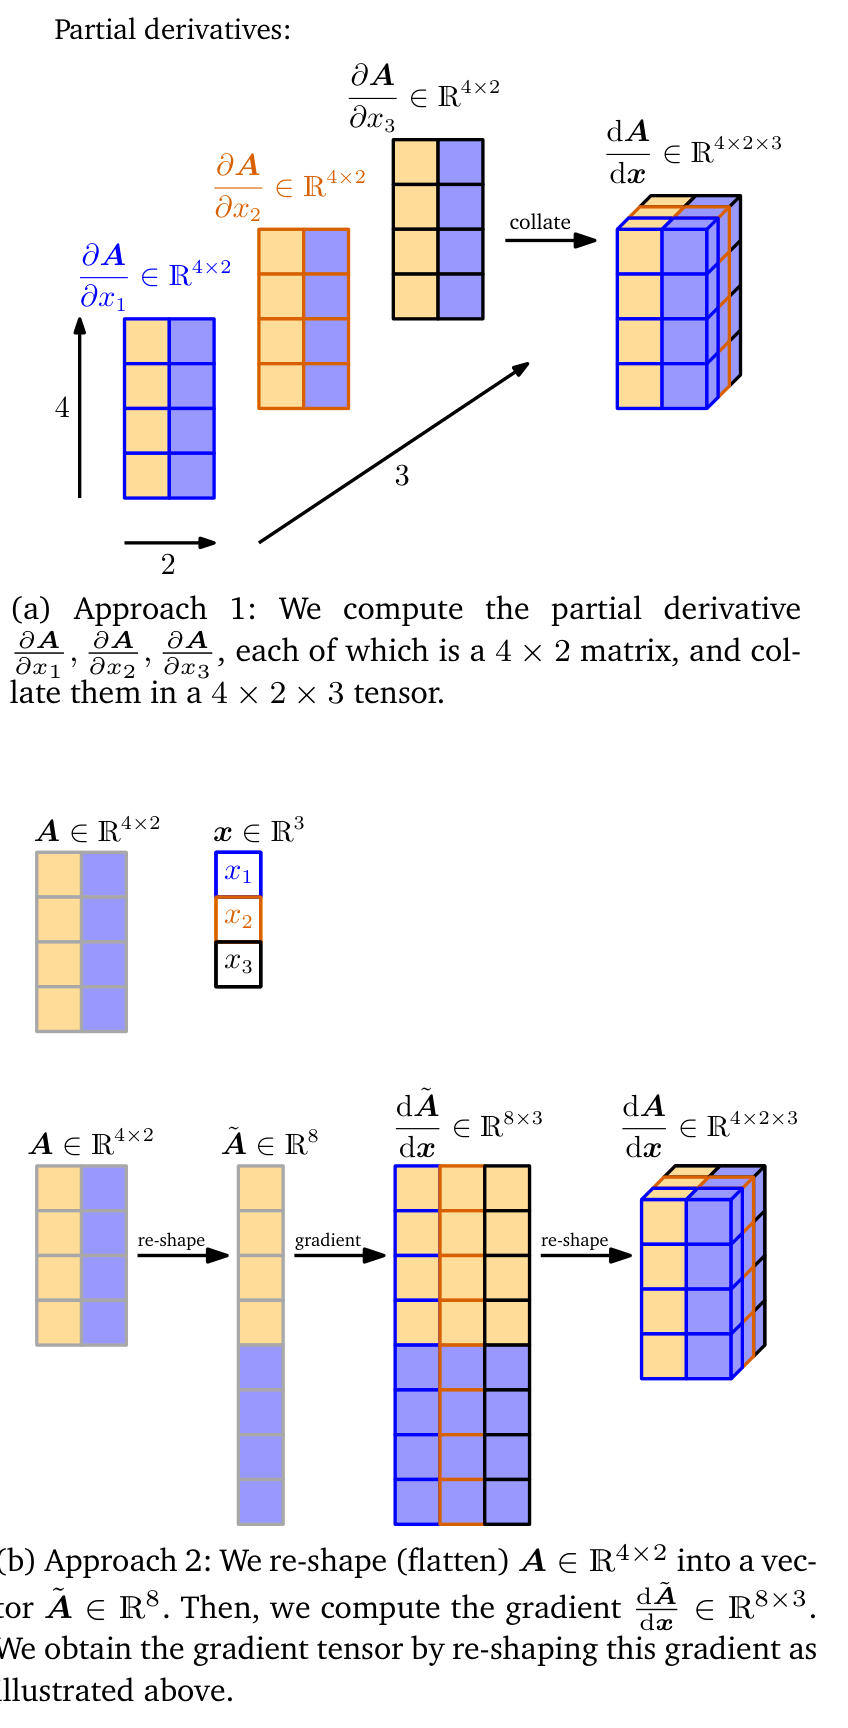
\includegraphics[width=0.66\textwidth,height=0.80\textheight,keepaspectratio]{docs/images/Figure5.7.png}
\caption*{\refstepcounter{figcounter}\label{fig:5-7}图~\thefigcounter 矩阵关于向量的梯度计算可视化。我们关注计算矩阵 A ∈ ℝ\textasciicircum{}(4×2) 关于向量 x ∈ ℝ\textasciicircum{}3 的梯度。已知梯度 dA/dx ∈ ℝ\textasciicircum{}(4×2×3)。我们采用两种等价方法得出结果：(a) 将偏导数整理为雅可比张量；(b) 将矩阵展平为向量，计算雅可比矩阵，再重塑为雅可比张量。}
\end{figure}


\begin{notebox}
\textbf{例 5.12（向量关于矩阵的梯度）}
\end{notebox}

\begin{notebox}
考虑以下示例：

\begin{equation}
\boldsymbol{f} = \boldsymbol{A} \boldsymbol{x}, \quad \boldsymbol{f} \in \mathbb{R}^M, \quad \boldsymbol{A} \in \mathbb{R}^{M \times N}, \quad \boldsymbol{x} \in \mathbb{R}^N
\tag{5.85}\label{eq:5-85}
\end{equation}

我们希望求梯度 $ \mathrm{d}\boldsymbol{f} / \mathrm{d}\boldsymbol{A} $。首先再次确定梯度的维度：

\begin{equation}
\frac{\mathrm{d}\boldsymbol{f}}{\mathrm{d}\boldsymbol{A}} \in \mathbb{R}^{M \times (M \times N)}
\tag{5.86}\label{eq:5-86}
\end{equation}

根据定义，梯度是偏导数的集合：

\begin{equation}
\begin{adjustbox}{max width=\linewidth}
\frac{\mathrm{d}\boldsymbol{f}}{\mathrm{d}\boldsymbol{A}} = \begin{bmatrix} \frac{\partial f_1}{\partial \boldsymbol{A}} \\ \vdots \\ \frac{\partial f_M}{\partial \boldsymbol{A}} \end{bmatrix}, \quad \frac{\partial f_i}{\partial \boldsymbol{A}} \in \mathbb{R}^{1 \times (M \times N)}
\end{adjustbox}
\tag{5.87}\label{eq:5-87}
\end{equation}

为了计算偏导数，显式写出矩阵-向量乘法会有所帮助：

\begin{equation}
f_i = \sum_{j=1}^N A_{ij} x_j, \quad i = 1, \ldots, M
\tag{5.88}\label{eq:5-88}
\end{equation}

偏导数由下式给出：

\begin{equation}
\frac{\partial f_i}{\partial A_{iq}} = x_q
\tag{5.89}\label{eq:5-89}
\end{equation}

这使我们能够计算 $ f_i $ 关于 $ \boldsymbol{A} $ 的某一行 $ \boldsymbol{A}_{i,:} $ 的偏导数：

\begin{equation}
\frac{\partial f_i}{\partial \boldsymbol{A}_{i,:}} = \boldsymbol{x}^\top \in \mathbb{R}^{1 \times 1 \times N}
\tag{5.90}\label{eq:5-90}
\end{equation}

\begin{equation}
\frac{\partial f_i}{\partial \boldsymbol{A}_{k \neq i,:}} = \boldsymbol{0}^\top \in \mathbb{R}^{1 \times 1 \times N}
\tag{5.91}\label{eq:5-91}
\end{equation}

这里我们必须注意正确的维度。由于 $ f_i $ 映射到 $ \mathbb{R} $，且 $ \boldsymbol{A} $ 的每一行大小为 $ 1 \times N $，因此 $ f_i $ 关于 $ \boldsymbol{A} $ 的一行的偏导数是一个大小为 $ 1 \times 1 \times N $ 的张量。 我们堆叠偏导数 (5.91)，通过下式得到式~\eqref{eq:5-87} 中所需的偏导数：

\begin{equation}
\begin{adjustbox}{max width=\linewidth}
\frac{\partial f_i}{\partial \boldsymbol{A}} = \begin{bmatrix} \boldsymbol{0}^\top \\ \vdots \\ \boldsymbol{0}^\top \\ \boldsymbol{x}^\top \\ \boldsymbol{0}^\top \\ \vdots \\ \boldsymbol{0}^\top \end{bmatrix} \in \mathbb{R}^{1 \times (M \times N)}
\end{adjustbox}
\tag{5.92}\label{eq:5-92}
\end{equation}
\end{notebox}

\begin{notebox}
\textbf{例 5.13（矩阵关于矩阵的梯度）}
\end{notebox}

\begin{notebox}
考虑矩阵 $ \boldsymbol{R} \in \mathbb{R}^{M \times N} $ 以及 $ \boldsymbol{f} : \mathbb{R}^{M \times N} \to \mathbb{R}^{N \times N} $，满足：

\begin{equation}
\boldsymbol{f}(\boldsymbol{R}) = \boldsymbol{R}^\top \boldsymbol{R} =: \boldsymbol{K} \in \mathbb{R}^{N \times N}
\tag{5.93}\label{eq:5-93}
\end{equation}

我们求梯度 $ \mathrm{d}\boldsymbol{K} / \mathrm{d}\boldsymbol{R} $。
\end{notebox}

\begin{notebox}
为了解决这个难题，我们首先写出已知的信息：该梯度的维度为：

\begin{equation}
\frac{\mathrm{d}\boldsymbol{K}}{\mathrm{d}\boldsymbol{R}} \in \mathbb{R}^{(N \times N) \times (M \times N)}
\tag{5.94}\label{eq:5-94}
\end{equation}

它是一个张量。此外，对于 $ p, q = 1, \ldots, N $：

\begin{equation}
\frac{\mathrm{d}K_{pq}}{\mathrm{d}\boldsymbol{R}} \in \mathbb{R}^{1 \times M \times N}
\tag{5.95}\label{eq:5-95}
\end{equation}

其中 $ K_{pq} $ 是 $ \boldsymbol{K} = \boldsymbol{f}(\boldsymbol{R}) $ 的第 $ (p, q) $ 个元素。将 $ \boldsymbol{R} $ 的第 $ i $ 列记为 $ \boldsymbol{r}_i $，则 $ \boldsymbol{K} $ 的每个元素由 $ \boldsymbol{R} $ 的两列的点积给出，即：

\begin{equation}
K_{pq} = \boldsymbol{r}_p^\top \boldsymbol{r}_q = \sum_{m=1}^M R_{mp} R_{mq}
\tag{5.96}\label{eq:5-96}
\end{equation}

现在计算偏导数 $ \frac{\partial K_{pq}}{\partial R_{ij}} $，得到：

\begin{equation}
\frac{\partial K_{pq}}{\partial R_{ij}} = \sum_{m=1}^M \frac{\partial}{\partial R_{ij}} R_{mp} R_{mq} = \partial_{pqij}
\tag{5.97}\label{eq:5-97}
\end{equation}

\begin{equation}
\partial_{pqij} = \begin{cases} R_{iq} & \textcn{若 } j = p, p \neq q \\ R_{ip} & \textcn{若 } j = q, p \neq q \\ 2R_{iq} & \textcn{若 } j = p, p = q \\ 0 & \textcn{其他情形} \end{cases}
\tag{5.98}\label{eq:5-98}
\end{equation}

由式~\eqref{eq:5-94} 可知，所求梯度的维度为 $ (N \times N) \times (M \times N) $，并且该张量的每个元素都由式~\eqref{eq:5-98} 中的 $ \partial_{pqij} $ 给出，其中 $ p, q, j = 1, \ldots, N $ 且 $ i = 1, \ldots, M $。
\end{notebox}

\section*{5.5 计算梯度的常用恒等式}
\addcontentsline{toc}{section}{5.5 计算梯度的常用恒等式}
\label{sec:5.5}

下面，我们列出一些在机器学习中经常需要的常用梯度恒等式（Petersen and Pedersen, 2012）。这里，我们用 $ \mathrm{tr}(\cdot) $ 表示迹（参见定义 4.4），用 $ \det(\cdot) $ 表示行列式（参见第 4.1 节），并用 $ \boldsymbol{f}(\boldsymbol{X})^{-1} $ 表示 $ \boldsymbol{f}(\boldsymbol{X}) $ 的逆（假定其存在）。

\begin{equation}
\frac{\partial}{\partial \boldsymbol{X}} \boldsymbol{f}(\boldsymbol{X})^\top = \left( \frac{\partial \boldsymbol{f}(\boldsymbol{X})}{\partial \boldsymbol{X}} \right)^\top
\tag{5.99}\label{eq:5-99}
\end{equation}

\begin{equation}
\frac{\partial}{\partial \boldsymbol{X}} \mathrm{tr}(\boldsymbol{f}(\boldsymbol{X})) = \mathrm{tr}\left( \frac{\partial \boldsymbol{f}(\boldsymbol{X})}{\partial \boldsymbol{X}} \right)
\tag{5.100}\label{eq:5-100}
\end{equation}

\begin{equation}
\begin{adjustbox}{max width=\linewidth}
\frac{\partial}{\partial \boldsymbol{X}} \det(\boldsymbol{f}(\boldsymbol{X})) = \det(\boldsymbol{f}(\boldsymbol{X})) \, \mathrm{tr}\left( \boldsymbol{f}(\boldsymbol{X})^{-1} \frac{\partial \boldsymbol{f}(\boldsymbol{X})}{\partial \boldsymbol{X}} \right)
\end{adjustbox}
\tag{5.101}\label{eq:5-101}
\end{equation}

\begin{equation}
\begin{adjustbox}{max width=\linewidth}
\frac{\partial}{\partial \boldsymbol{X}} \boldsymbol{f}(\boldsymbol{X})^{-1} = -\boldsymbol{f}(\boldsymbol{X})^{-1} \frac{\partial \boldsymbol{f}(\boldsymbol{X})}{\partial \boldsymbol{X}} \boldsymbol{f}(\boldsymbol{X})^{-1}
\end{adjustbox}
\tag{5.102}\label{eq:5-102}
\end{equation}

\begin{equation}
\frac{\partial \boldsymbol{a}^\top \boldsymbol{X}^{-1} \boldsymbol{b}}{\partial \boldsymbol{X}} = -(\boldsymbol{X}^{-1})^\top \boldsymbol{a} \boldsymbol{b}^\top (\boldsymbol{X}^{-1})^\top
\tag{5.103}\label{eq:5-103}
\end{equation}

\begin{equation}
\frac{\partial \boldsymbol{x}^\top \boldsymbol{a}}{\partial \boldsymbol{x}} = \boldsymbol{a}^\top
\tag{5.104}\label{eq:5-104}
\end{equation}

\begin{equation}
\frac{\partial \boldsymbol{a}^\top \boldsymbol{x}}{\partial \boldsymbol{x}} = \boldsymbol{a}^\top
\tag{5.105}\label{eq:5-105}
\end{equation}

\begin{equation}
\frac{\partial \boldsymbol{a}^\top \boldsymbol{X} \boldsymbol{b}}{\partial \boldsymbol{X}} = \boldsymbol{a} \boldsymbol{b}^\top
\tag{5.106}\label{eq:5-106}
\end{equation}

\begin{equation}
\frac{\partial \boldsymbol{x}^\top \boldsymbol{B} \boldsymbol{x}}{\partial \boldsymbol{x}} = \boldsymbol{x}^\top (\boldsymbol{B} + \boldsymbol{B}^\top)
\tag{5.107}\label{eq:5-107}
\end{equation}

\begin{equation}
\begin{adjustbox}{max width=\linewidth}
\frac{\partial}{\partial \boldsymbol{s}} (\boldsymbol{x} - \boldsymbol{A} \boldsymbol{s})^\top \boldsymbol{W} (\boldsymbol{x} - \boldsymbol{A} \boldsymbol{s}) = -2(\boldsymbol{x} - \boldsymbol{A} \boldsymbol{s})^\top \boldsymbol{W} \boldsymbol{A} \quad (\textcn{对于对称矩阵 } \boldsymbol{W})
\end{adjustbox}
\tag{5.108}\label{eq:5-108}
\end{equation}

\emph{备注} 。在本书中，我们仅讨论矩阵的迹和转置。然而，我们已经看到导数可以是更高维的张量，在那种情况下通常的迹和转置并没有定义。在这些情况下，$ D \times D \times E \times F $ 维张量的迹将是一个 $ E \times F $ 维矩阵。这是 \emph{张量缩并（tensor contraction）} 的特例。类似地，当我们对张量进行“转置”时，我们的意思是对换前两个维度。具体而言，在式~\eqref{eq:5-99} 至式~\eqref{eq:5-102} 中，当我们处理多元函数 $ \boldsymbol{f}(\cdot) $ 并计算关于矩阵的导数时（并且选择不按照第 5.4 节讨论的那样将其向量化），需要进行与张量相关的计算。♦

\section*{5.6 反向传播与自动微分}
\addcontentsline{toc}{section}{5.6 反向传播与自动微分}
\label{sec:5.6}

在许多机器学习应用中，我们通过执行梯度下降（第 7.1 节）来寻找良好的模型参数，这依赖于我们能够计算学习目标相对于模型参数的梯度这一事实。对于给定的目标函数，我们可以利用微积分并应用链式法则（参见第 5.2.2 节）来获得相对于模型参数的梯度。在第 5.3 节中，当考察平方损失相对于线性回归模型参数的梯度时，我们已经初步体会到了这一点。

\emph{备注} 。关于反向传播与链式法则的讨论，亦可参阅 Tim Vieira 的博文：\href{https://tinyurl.com/ycfm2yrw}{https://tinyurl.com/ycfm2yrw}。♦

考虑函数：

\begin{equation}
f(x) = \sqrt{x^2 + \exp(x^2)} + \cos(x^2 + \exp(x^2))
\tag{5.109}\label{eq:5-109}
\end{equation}

通过应用链式法则，并注意到微分是线性的，我们计算梯度：

\begin{equation}
\begin{adjustbox}{max width=\linewidth}
\begin{aligned}
\frac{\mathrm{d}f}{\mathrm{d}x} &= \frac{2x + 2x \exp(x^2)}{2\sqrt{x^2 + \exp(x^2)}} - \sin(x^2 + \exp(x^2))(2x + 2x \exp(x^2)) \\
&= 2x \left( \frac{1}{2\sqrt{x^2 + \exp(x^2)}} - \sin(x^2 + \exp(x^2)) \right) (1 + \exp(x^2))
\end{aligned}
\end{adjustbox}
\tag{5.110}\label{eq:5-110}
\end{equation}

以这种显式方式写出梯度通常是不切实际的，因为它往往会导致非常冗长的导数表达式。在实践中，这意味着如果我们不够谨慎，梯度的实现开销可能会显著高于计算函数本身的开销，从而带来不必要的计算负担。对于训练深度神经网络模型， \emph{反向传播（backpropagation）} 算法（Kelley, 1960; Bryson, 1961; Dreyfus, 1962; Rumelhart et al., 1986）是一种计算误差函数相对于模型参数梯度的有效方法。

\medskip\hrule\medskip

\section*{5.6.1 深度网络中的梯度}
\addcontentsline{toc}{subsection}{5.6.1 深度网络中的梯度}

链式法则被发挥到极致的一个领域是深度学习，其中函数值 $ \boldsymbol{y} $ 是通过多层函数复合计算得到的：

\begin{equation}
\boldsymbol{y} = (f_K \circ f_{K-1} \circ \cdots \circ f_1)(\boldsymbol{x}) = f_K(f_{K-1}(\cdots (f_1(\boldsymbol{x})) \cdots ))
\tag{5.111}\label{eq:5-111}
\end{equation}

其中 $ \boldsymbol{x} $ 是输入（例如图像），$ \boldsymbol{y} $ 是观测值（例如类别标签），每个函数 $ f_i $（$ i = 1, \ldots, K $）都拥有其自身的参数。


\begin{figure}[H]
\centering
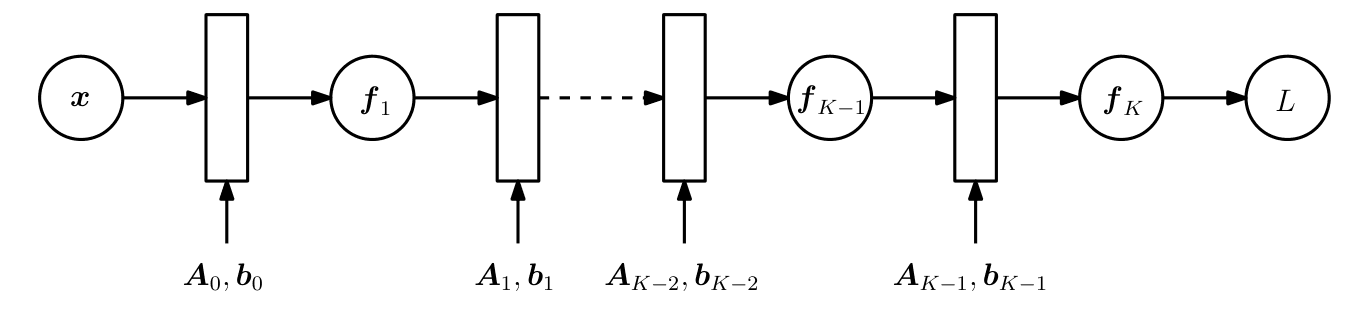
\includegraphics[width=0.92\textwidth,keepaspectratio]{docs/images/Figure5.8.png}
\caption*{\refstepcounter{figcounter}\label{fig:5-8}图~\thefigcounter 多层神经网络中的前向传播，用于将损失 L 计算为输入 x 和参数 Aᵢ, bᵢ 的函数。}
\end{figure}


在多层神经网络中，我们在第 $ i $ 层拥有函数 $ f_i(\boldsymbol{x}_{i-1}) = \sigma(\boldsymbol{A}_{i-1}\boldsymbol{x}_{i-1} + \boldsymbol{b}_{i-1}) $（为了使记号更简洁，我们假定各层的激活函数相同）。这里 $ \boldsymbol{x}_{i-1} $ 是第 $ i-1 $ 层的输出，$ \sigma $ 是 \emph{激活函数（activation function）} ，例如逻辑 S 形函数（logistic sigmoid）$ \frac{1}{1 + \mathrm{e}^{-x}} $、双曲正切函数（$ \tanh $）或整流线性单元（rectified linear unit, ReLU）。为了训练这些模型，我们需要损失函数 $ L $ 相对于所有模型参数 $ \boldsymbol{A}_j, \boldsymbol{b}_j $（$ j = 0, \ldots, K-1 $）的梯度。这也要求我们计算 $ L $ 相对于每一层输入的梯度。例如，如果我们有输入 $ \boldsymbol{x} $ 和观测值 $ \boldsymbol{y} $，以及由以下公式定义的网络结构：

\begin{equation}
\boldsymbol{f}_0 := \boldsymbol{x}
\tag{5.112}\label{eq:5-112}
\end{equation}

\begin{equation}
\boldsymbol{f}_i := \sigma_i(\boldsymbol{A}_{i-1}\boldsymbol{f}_{i-1} + \boldsymbol{b}_{i-1}) , \quad i = 1, \ldots, K
\tag{5.113}\label{eq:5-113}
\end{equation}

（参见图~\ref{fig:5-8} 的可视化），我们可能希望找到参数 $ \boldsymbol{A}_j, \boldsymbol{b}_j $（$ j = 0, \ldots, K-1 $），使得平方损失：

\begin{equation}
L(\boldsymbol{\theta}) = \|\boldsymbol{y} - \boldsymbol{f}_K(\boldsymbol{\theta}, \boldsymbol{x})\|^2
\tag{5.114}\label{eq:5-114}
\end{equation}

最小化，其中 $ \boldsymbol{\theta} = \{\boldsymbol{A}_0, \boldsymbol{b}_0, \ldots, \boldsymbol{A}_{K-1}, \boldsymbol{b}_{K-1}\} $。

为了获得相对于参数集 $ \boldsymbol{\theta} $ 的梯度，我们需要 $ L $ 相对于每一层参数 $ \boldsymbol{\theta}_j = \{\boldsymbol{A}_j, \boldsymbol{b}_j\} $（$ j = 0, \ldots, K-1 $）的偏导数。链式法则允许我们将这些偏导数确定为：

\begin{equation}
\frac{\partial L}{\partial \boldsymbol{\theta}_{K-1}} = \frac{\partial L}{\partial \boldsymbol{f}_K} {\color{blue}\frac{\partial \boldsymbol{f}_K}{\partial \boldsymbol{\theta}_{K-1}}}
\tag{5.115}\label{eq:5-115}
\end{equation}

\begin{equation}
\begin{adjustbox}{max width=\linewidth}
\frac{\partial L}{\partial \boldsymbol{\theta}_{K-2}} = \frac{\partial L}{\partial \boldsymbol{f}_K} \boxed{{\color{orange}\frac{\partial \boldsymbol{f}_K}{\partial \boldsymbol{f}_{K-1}}} {\color{blue}\frac{\partial \boldsymbol{f}_{K-1}}{\partial \boldsymbol{\theta}_{K-2}}}}
\end{adjustbox}
\tag{5.116}\label{eq:5-116}
\end{equation}

\begin{equation}
\begin{adjustbox}{max width=\linewidth}
\frac{\partial L}{\partial \boldsymbol{\theta}_{K-3}} = \frac{\partial L}{\partial \boldsymbol{f}_K} {\color{orange}\frac{\partial \boldsymbol{f}_K}{\partial \boldsymbol{f}_{K-1}}} \boxed{{\color{orange}\frac{\partial \boldsymbol{f}_{K-1}}{\partial \boldsymbol{f}_{K-2}}} {\color{blue}\frac{\partial \boldsymbol{f}_{K-2}}{\partial \boldsymbol{\theta}_{K-3}}}}
\end{adjustbox}
\tag{5.117}\label{eq:5-117}
\end{equation}

\begin{equation}
\begin{adjustbox}{max width=\linewidth}
\frac{\partial L}{\partial \boldsymbol{\theta}_i} = \frac{\partial L}{\partial \boldsymbol{f}_K} {\color{orange}\frac{\partial \boldsymbol{f}_K}{\partial \boldsymbol{f}_{K-1}}} \cdots \boxed{{\color{orange}\frac{\partial \boldsymbol{f}_{i+2}}{\partial \boldsymbol{f}_{i+1}}} {\color{blue}\frac{\partial \boldsymbol{f}_{i+1}}{\partial \boldsymbol{\theta}_i}}}
\end{adjustbox}
\tag{5.118}\label{eq:5-118}
\end{equation}

其中橙色项是某一层输出相对于其输入的偏导数，而蓝色项是某一层输出相对于其参数的偏导数。假设我们已经计算了偏导数 $ \partial L / \partial \boldsymbol{\theta}_{i+1} $，那么大部分计算都可以复用于计算 $ \partial L / \partial \boldsymbol{\theta}_i $。我们需要额外计算的项由方框标出。图~\ref{fig:5-9} 直观展示了梯度是如何在网络中反向传递的。

\emph{备注} 。关于神经网络梯度的更深入讨论可参见 Justin Domke 的讲义：\href{https://tinyurl.com/yalcxgtv}{https://tinyurl.com/yalcxgtv}。♦


\begin{figure}[H]
\centering
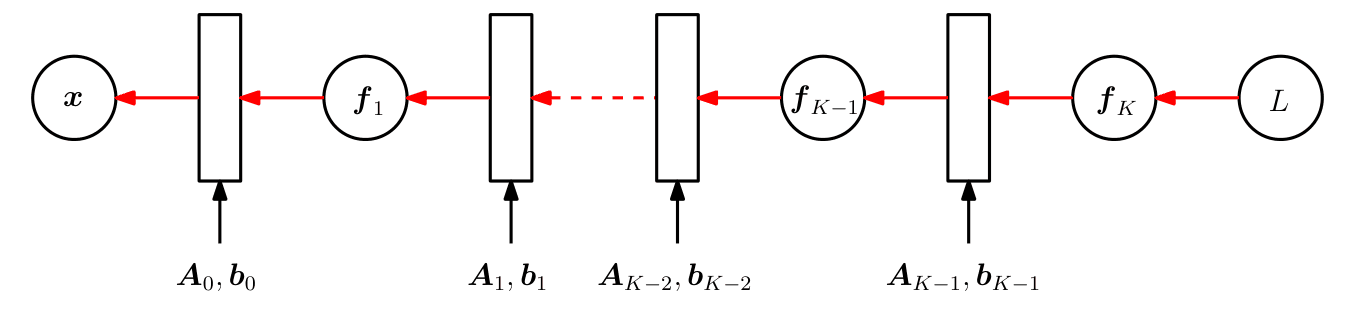
\includegraphics[width=0.92\textwidth,keepaspectratio]{docs/images/Figure5.9.png}
\caption*{\refstepcounter{figcounter}\label{fig:5-9}图~\thefigcounter 多层神经网络中的反向传播，用于计算损失函数的梯度。}
\end{figure}


\medskip\hrule\medskip

\section*{5.6.2 自动微分}
\addcontentsline{toc}{subsection}{5.6.2 自动微分}

事实证明，反向传播是数值分析中一种称为 \emph{自动微分（automatic differentiation）} 的通用技术的特例。我们可以将自动微分视为一组通过处理中间变量并应用链式法则，在数值上（与符号微分相对）评估函数精确（达到机器精度）梯度的技术。自动微分应用一系列基本算术运算（如加法和乘法）以及初等函数（如 $ \sin, \cos, \exp, \log $）。通过对这些运算应用链式法则，可以自动计算相当复杂的函数的梯度。自动微分适用于通用计算机程序，并且具有前向模式和反向模式。Baydin 等人（Baydin et al., 2018）对机器学习中的自动微分给出了精彩的综述。

\emph{备注} 。自动微分不同于符号微分以及梯度的数值近似（例如使用有限差分）。♦


\begin{figure}[H]
\centering

\includegraphics[width=0.92\textwidth,keepaspectratio]{docs/images/Figure5.10.png}
\caption*{\refstepcounter{figcounter}\label{fig:5-10}图~\thefigcounter 说明数据通过一些中间变量 a, b 从 x 流向 y 的简单计算图。}
\end{figure}


图~\ref{fig:5-10} 展示了一个简单的计算图，表示数据通过一些中间变量 $ a, b $ 从输入 $ x $ 流向输出 $ y $。如果我们要计算导数 $ \mathrm{d}y/\mathrm{d}x $，我们将应用链式法则并得到：

\begin{equation}
\frac{\mathrm{d}y}{\mathrm{d}x} = \frac{\mathrm{d}y}{\mathrm{d}b} \frac{\mathrm{d}b}{\mathrm{d}a} \frac{\mathrm{d}a}{\mathrm{d}x} .
\tag{5.119}\label{eq:5-119}
\end{equation}

直观上，前向模式与反向模式的区别在于乘法的计算顺序（在一般情况下，我们处理的是雅可比矩阵，它们可以是向量、矩阵或张量）。由于矩阵乘法的结合律，我们可以在以下两者之间进行选择：

\begin{equation}
\frac{\mathrm{d}y}{\mathrm{d}x} = \left( \frac{\mathrm{d}y}{\mathrm{d}b} \frac{\mathrm{d}b}{\mathrm{d}a} \right) \frac{\mathrm{d}a}{\mathrm{d}x}
\tag{5.120}\label{eq:5-120}
\end{equation}

\begin{equation}
\frac{\mathrm{d}y}{\mathrm{d}x} = \frac{\mathrm{d}y}{\mathrm{d}b} \left( \frac{\mathrm{d}b}{\mathrm{d}a} \frac{\mathrm{d}a}{\mathrm{d}x} \right) .
\tag{5.121}\label{eq:5-121}
\end{equation}

式~\eqref{eq:5-120} 即为 \emph{反向模式（reverse mode）} ，因为梯度在计算图中反向传播，即与数据流的方向相反。式~\eqref{eq:5-121} 则为 \emph{前向模式（forward mode）} ，其中梯度随着数据从左到右流经计算图。

在下文中，我们将重点关注反向模式自动微分，即反向传播。在神经网络的背景下，输入的维度往往远高于标签的维度，因此反向模式在计算上要比前向模式经济得多。让我们从一个启发性的示例开始。

\begin{notebox}
\textbf{例 5.14}
\end{notebox}

\begin{notebox}
考虑来自式~\eqref{eq:5-109} 的函数：

\begin{equation}
f(x) = \sqrt{x^2 + \exp(x^2)} + \cos(x^2 + \exp(x^2))
\tag{5.122}\label{eq:5-122}
\end{equation}

如果我们在计算机上实现函数 $ f $，可以通过引入 \emph{中间变量（intermediate variables）} 来节省部分计算：

\begin{equation}
a = x^2
\tag{5.123}\label{eq:5-123}
\end{equation}

\begin{equation}
b = \exp(a)
\tag{5.124}\label{eq:5-124}
\end{equation}

\begin{equation}
c = a + b
\tag{5.125}\label{eq:5-125}
\end{equation}

\begin{equation}
d = \sqrt{c}
\tag{5.126}\label{eq:5-126}
\end{equation}

\begin{equation}
e = \cos(c)
\tag{5.127}\label{eq:5-127}
\end{equation}

\begin{equation}
f = d + e .
\tag{5.128}\label{eq:5-128}
\end{equation}
\end{notebox}

\begin{notebox}

\begin{figure}[H]
\centering
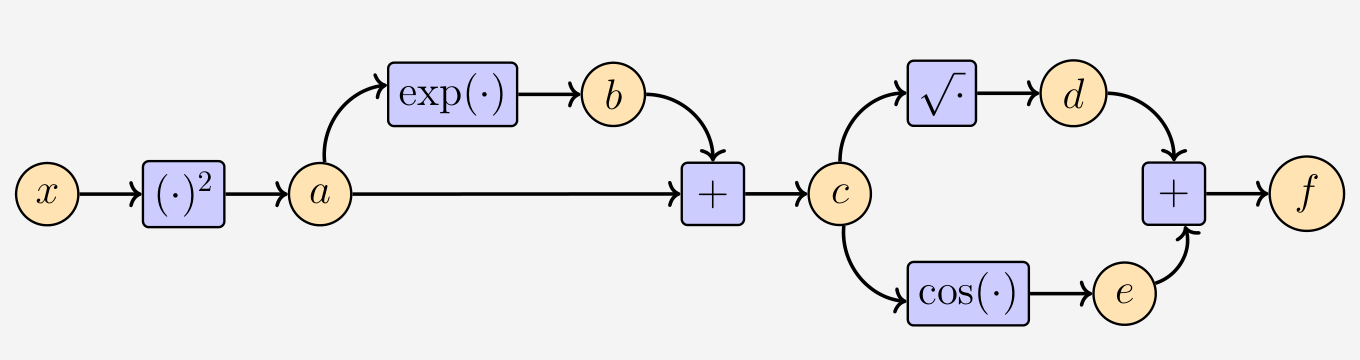
\includegraphics[width=0.92\textwidth,keepaspectratio]{docs/images/Figure5.11.png}
\caption*{\refstepcounter{figcounter}\label{fig:5-11}图~\thefigcounter 包含输入 x、函数值 f 以及中间变量 a, b, c, d, e 的计算图。}
\end{figure}

\end{notebox}

\begin{notebox}
这与应用链式法则时的思维过程完全相同。请注意，上述方程组所需的运算次数少于直接实现式~\eqref{eq:5-109} 中定义的函数 $ f(x) $ 所需的运算次数。图~\ref{fig:5-11} 中对应的计算图展示了获得函数值 $ f $ 所需的数据流与计算过程。
\end{notebox}

\begin{notebox}
包含中间变量的方程组可以被视为一个计算图，这种表示形式在神经网络软件库的实现中得到了广泛应用。通过回顾初等函数导数的定义，我们可以直接计算中间变量相对于其对应输入的导数。我们得到以下结果：

\begin{equation}
\frac{\partial a}{\partial x} = 2x
\tag{5.129}\label{eq:5-129}
\end{equation}

\begin{equation}
\frac{\partial b}{\partial a} = \exp(a)
\tag{5.130}\label{eq:5-130}
\end{equation}

\begin{equation}
\frac{\partial c}{\partial a} = 1 = \frac{\partial c}{\partial b}
\tag{5.131}\label{eq:5-131}
\end{equation}

\begin{equation}
\frac{\partial d}{\partial c} = \frac{1}{2\sqrt{c}}
\tag{5.132}\label{eq:5-132}
\end{equation}

\begin{equation}
\frac{\partial e}{\partial c} = -\sin(c)
\tag{5.133}\label{eq:5-133}
\end{equation}

\begin{equation}
\frac{\partial f}{\partial d} = 1 = \frac{\partial f}{\partial e} .
\tag{5.134}\label{eq:5-134}
\end{equation}

通过观察图~\ref{fig:5-11} 中的计算图，我们可以从输出端向后推导来计算 $ \partial f/\partial x $，并得到：

\begin{equation}
\frac{\partial f}{\partial c} = \frac{\partial f}{\partial d} \frac{\partial d}{\partial c} + \frac{\partial f}{\partial e} \frac{\partial e}{\partial c}
\tag{5.135}\label{eq:5-135}
\end{equation}

\begin{equation}
\frac{\partial f}{\partial b} = \frac{\partial f}{\partial c} \frac{\partial c}{\partial b}
\tag{5.136}\label{eq:5-136}
\end{equation}

\begin{equation}
\frac{\partial f}{\partial a} = \frac{\partial f}{\partial b} \frac{\partial b}{\partial a} + \frac{\partial f}{\partial c} \frac{\partial c}{\partial a}
\tag{5.137}\label{eq:5-137}
\end{equation}

\begin{equation}
\frac{\partial f}{\partial x} = \frac{\partial f}{\partial a} \frac{\partial a}{\partial x} .
\tag{5.138}\label{eq:5-138}
\end{equation}

请注意，我们隐式地应用了链式法则来求得 $ \partial f/\partial x $。通过代入初等函数导数的结果，我们得到：

\begin{equation}
\frac{\partial f}{\partial c} = 1 \cdot \frac{1}{2\sqrt{c}} + 1 \cdot (-\sin(c))
\tag{5.139}\label{eq:5-139}
\end{equation}

\begin{equation}
\frac{\partial f}{\partial b} = \frac{\partial f}{\partial c} \cdot 1
\tag{5.140}\label{eq:5-140}
\end{equation}

\begin{equation}
\frac{\partial f}{\partial a} = \frac{\partial f}{\partial b} \exp(a) + \frac{\partial f}{\partial c} \cdot 1
\tag{5.141}\label{eq:5-141}
\end{equation}

\begin{equation}
\frac{\partial f}{\partial x} = \frac{\partial f}{\partial a} \cdot 2x .
\tag{5.142}\label{eq:5-142}
\end{equation}

将上述每个导数视为一个变量，我们发现计算导数所需的计算复杂度与计算函数本身的复杂度相当。这是相当反直觉的，因为导数 $ \partial f/\partial x $ 的数学表达式~\eqref{eq:5-110} 显著比式~\eqref{eq:5-109} 中函数 $ f(x) $ 的数学表达式要复杂得多。
\end{notebox}

自动微分是例 5.14 的形式化推广。设 $ x_1, \ldots, x_d $ 为函数的输入变量，$ x_{d+1}, \ldots, x_{D-1} $ 为中间变量，而 $ x_D $ 为输出变量。则计算图可表示如下：

对于 $ i = d + 1, \ldots, D $：

\begin{equation}
x_i = g_i(\boldsymbol{x}_{\mathrm{Pa}(x_i)})
\tag{5.143}\label{eq:5-143}
\end{equation}

其中 $ g_i(\cdot) $ 为初等函数，而 $ \boldsymbol{x}_{\mathrm{Pa}(x_i)} $ 是变量 $ x_i $ 在图中的父节点集合。给定以此种方式定义的函数，我们可以逐步应用链式法则来计算函数的导数。回顾根据定义 $ f = x_D $，因此：

\begin{equation}
\frac{\partial f}{\partial x_D} = 1 .
\tag{5.144}\label{eq:5-144}
\end{equation}

对于其他变量 $ x_i $，我们应用链式法则：

\begin{equation}
\begin{adjustbox}{max width=\linewidth}
\frac{\partial f}{\partial x_i} = \sum_{x_j : x_i \in \mathrm{Pa}(x_j)} \frac{\partial f}{\partial x_j} \frac{\partial x_j}{\partial x_i} = \sum_{x_j : x_i \in \mathrm{Pa}(x_j)} \frac{\partial f}{\partial x_j} \frac{\partial g_j}{\partial x_i}
\end{adjustbox}
\tag{5.145}\label{eq:5-145}
\end{equation}

其中 $ \mathrm{Pa}(x_j) $ 是计算图中 $ x_j $ 的父节点集合。式~\eqref{eq:5-143} 是函数的前向传播，而式~\eqref{eq:5-145} 则是梯度在计算图中的反向传播（反向模式的自动微分需要一棵解析树）。在神经网络训练中，我们反向传播预测相对于标签的误差。

上述自动微分方法在函数可以表示为初等函数可微的计算图时均适用。事实上，该函数甚至不必是纯数学函数，也可以是一个计算机程序。然而，并非所有计算机程序都可以进行自动微分，例如当我们无法找到可微的初等函数时。诸如 for 循环和 if 条件语句等编程结构也需要格外小心处理。

\section*{5.7 高阶导数}
\addcontentsline{toc}{section}{5.7 高阶导数}
\label{sec:5.7}

到目前为止，我们讨论了梯度，即一阶导数。有时，我们会对更高阶的导数感兴趣，例如，当我们想要使用 \emph{牛顿法（Newton's method）} 进行优化时，这需要二阶导数 (Nocedal and Wright, 2006)。在第 5.1.1 节中，我们讨论了利用多项式逼近函数的泰勒级数。在多元情形下，我们也可以做完全相同的事情。接下来，我们将正式展开这部分内容。但首先让我们从一些记号开始。

考虑含有两个变量 $ x, y $ 的函数 $ f : \mathbb{R}^2 \to \mathbb{R} $。我们对高阶偏导数（以及梯度）使用以下记号：

\begin{itemize}
\item $ \frac{\partial^2 f}{\partial x^2} $ 是 $ f $ 关于 $ x $ 的二阶偏导数。
\item $ \frac{\partial^n f}{\partial x^n} $ 是 $ f $ 关于 $ x $ 的 $ n $ 阶偏导数。
\item $ \frac{\partial^2 f}{\partial y \partial x} = \frac{\partial}{\partial y} \left( \frac{\partial f}{\partial x} \right) $ 是先关于 $ x $ 求偏导、再关于 $ y $ 求偏导所得到的偏导数。
\item $ \frac{\partial^2 f}{\partial x \partial y} $ 是先关于 $ y $ 求偏导、再关于 $ x $ 求偏导所得到的偏导数。
\end{itemize}

\emph{黑塞矩阵（Hessian）} 是所有二阶偏导数的集合。

如果 $ f(x, y) $ 是二次（连续）可微函数，则：

\begin{equation}
\frac{\partial^2 f}{\partial x \partial y} = \frac{\partial^2 f}{\partial y \partial x}
\tag{5.146}\label{eq:5-146}
\end{equation}

即求导的顺序无关紧要，且对应的 \emph{黑塞矩阵（Hessian matrix）} ：

\begin{equation}
\boldsymbol{H} = \begin{bmatrix} \frac{\partial^2 f}{\partial x^2} & \frac{\partial^2 f}{\partial x \partial y} \\ \frac{\partial^2 f}{\partial x \partial y} & \frac{\partial^2 f}{\partial y^2} \end{bmatrix}
\tag{5.147}\label{eq:5-147}
\end{equation}

是对称的。黑塞矩阵记为 $ \nabla_{x,y}^2 f(x, y) $。一般地，对于 $ \boldsymbol{x} \in \mathbb{R}^n $ 和 $ f : \mathbb{R}^n \to \mathbb{R} $，黑塞矩阵是一个 $ n \times n $ 矩阵。黑塞矩阵衡量了函数在 $ (x, y) $ 邻域内的局部曲率。

\emph{备注} （向量场的黑塞矩阵）。如果 $ \boldsymbol{f} : \mathbb{R}^n \to \mathbb{R}^m $ 是一个向量场，则黑塞矩阵是一个 $ (m \times n \times n) $ 阶张量。♦

\section*{5.8 线性化与多元泰勒级数}
\addcontentsline{toc}{section}{5.8 线性化与多元泰勒级数}
\label{sec:5.8}

函数 $ f $ 的梯度 $ \nabla f $ 经常用于在 $ \boldsymbol{x}_0 $ 附近对 $ f $ 进行局部线性逼近：

\begin{equation}
f(\boldsymbol{x}) \approx f(\boldsymbol{x}_0) + (\nabla_{\boldsymbol{x}} f)(\boldsymbol{x}_0)(\boldsymbol{x} - \boldsymbol{x}_0)
\tag{5.148}\label{eq:5-148}
\end{equation}

这里 $ (\nabla_{\boldsymbol{x}} f)(\boldsymbol{x}_0) $ 是 $ f $ 关于 $ \boldsymbol{x} $ 在 $ \boldsymbol{x}_0 $ 处求值的梯度。


\begin{figure}[H]
\centering
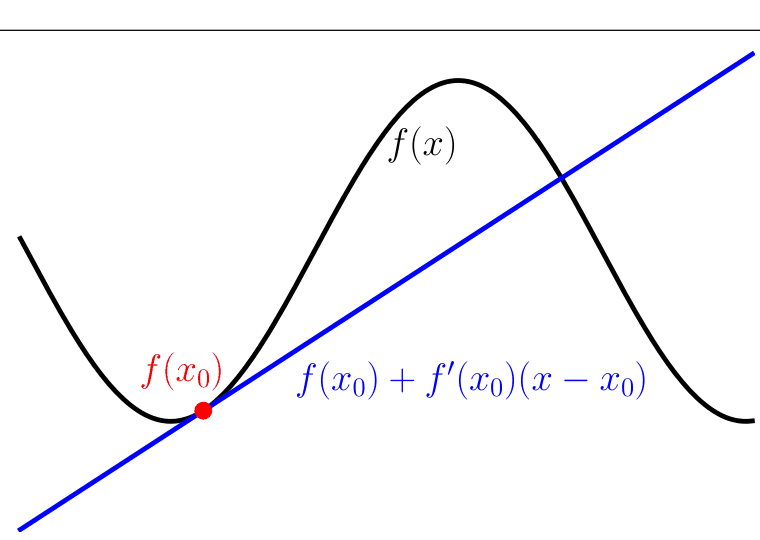
\includegraphics[width=0.92\textwidth,keepaspectratio]{docs/images/Figure5.12.png}
\caption*{\refstepcounter{figcounter}\label{fig:5-12}图~\thefigcounter 函数的线性逼近。原函数 f 在 x₀ = -2 处使用一阶泰勒级数展开进行线性化。}
\end{figure}


图~\ref{fig:5-12} 说明了函数 $ f $ 在输入 $ \boldsymbol{x}_0 $ 处的线性逼近。原函数由一条直线逼近。这种逼近在局部是精确的，但随着我们离 $ \boldsymbol{x}_0 $ 越来越远，逼近效果会变差。式~\eqref{eq:5-148} 是 $ f $ 在 $ \boldsymbol{x}_0 $ 处的多元泰勒级数展开的特例，其中我们仅考虑了前两项。下面我们将讨论更一般的情形，这将实现更好的逼近。


\begin{figure}[H]
\centering
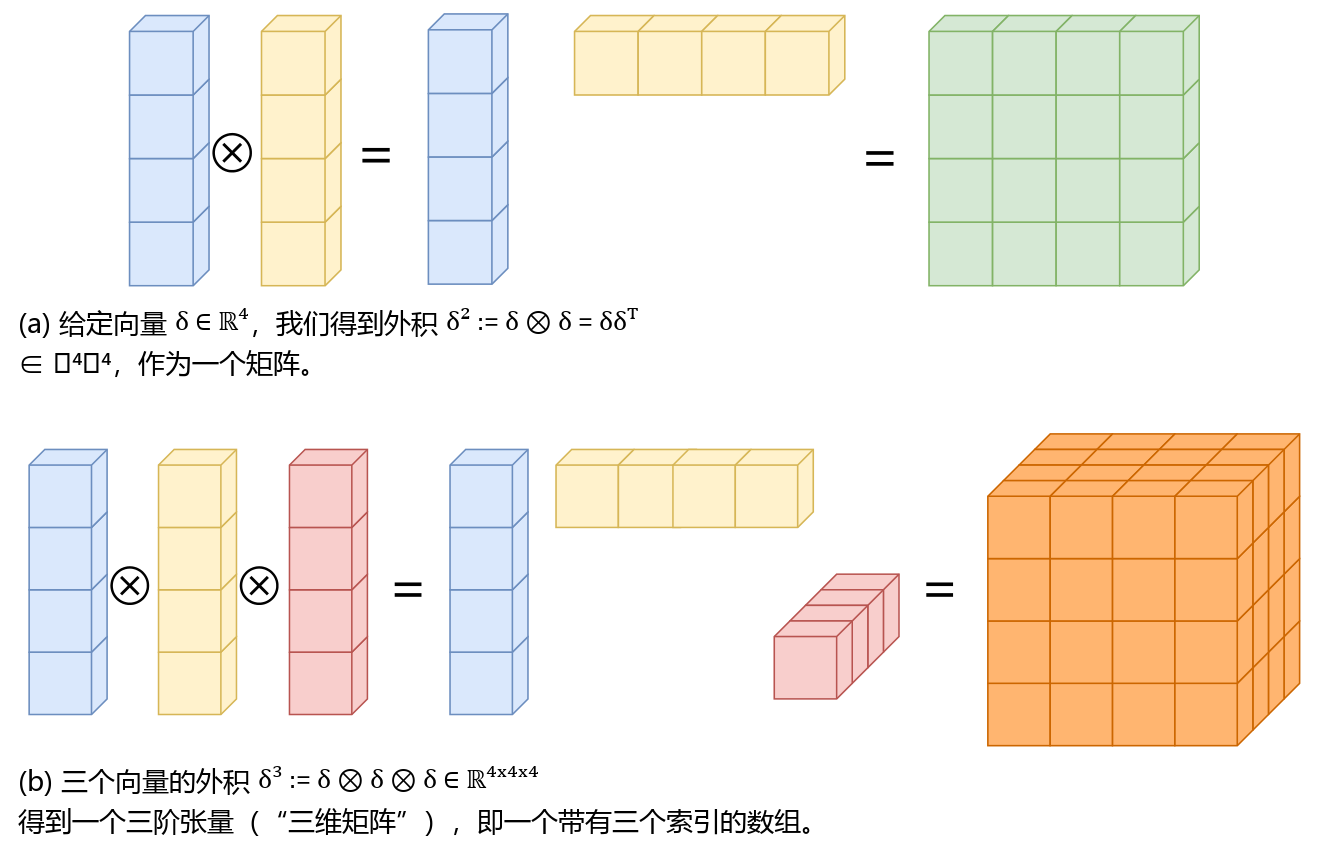
\includegraphics[width=0.92\textwidth,keepaspectratio]{docs/images/Figure5.13.png}
\caption*{\refstepcounter{figcounter}\label{fig:5-13}图~\thefigcounter 外积的可视化。向量的外积使数组的维度每项增加 1。(a) 两个向量的外积得到一个矩阵；(b) 三个向量的外积产生一个三阶张量。(a) 给定向量 δ ∈ ℝ⁴，我们获得外积 δ² := δ ⊗ δ = δδᵀ ∈ ℝ⁴ˣ⁴ 作为矩阵。(b) 外积 δ³ := δ ⊗ δ ⊗ δ ∈ ℝ⁴ˣ⁴ˣ⁴ 得到一个三阶张量（“三维矩阵”），即带有三个索引的数组。}
\end{figure}


\textbf{定义 5.7}（多元泰勒级数）。考虑一个在 $ \boldsymbol{x}_0 $ 处光滑的函数：

\begin{equation}
f : \mathbb{R}^D \to \mathbb{R}
\tag{5.149}\label{eq:5-149}
\end{equation}

\begin{equation}
\boldsymbol{x} \mapsto f(\boldsymbol{x}), \quad \boldsymbol{x} \in \mathbb{R}^D
\tag{5.150}\label{eq:5-150}
\end{equation}

当我们定义差向量 $ \boldsymbol{\delta} := \boldsymbol{x} - \boldsymbol{x}_0 $ 时，$ f $ 在 $ \boldsymbol{x}_0 $ 处的 \emph{多元泰勒级数（multivariate Taylor series）} 定义为：

\begin{equation}
f(\boldsymbol{x}) = \sum_{k=0}^\infty \frac{D_{\boldsymbol{x}}^k f(\boldsymbol{x}_0)}{k!} \boldsymbol{\delta}^k
\tag{5.151}\label{eq:5-151}
\end{equation}

其中 $ D_{\boldsymbol{x}}^k f(\boldsymbol{x}_0) $ 是 $ f $ 关于 $ \boldsymbol{x} $ 在 $ \boldsymbol{x}_0 $ 处的 $ k $ 阶（全）导数。

\textbf{定义 5.8}（泰勒多项式）。$ f $ 在 $ \boldsymbol{x}_0 $ 处的 $ n $ 次 \emph{泰勒多项式（Taylor polynomial）} 包含式~\eqref{eq:5-151} 级数中的前 $ n + 1 $ 项，定义为：

\begin{equation}
T_n(\boldsymbol{x}) = \sum_{k=0}^n \frac{D_{\boldsymbol{x}}^k f(\boldsymbol{x}_0)}{k!} \boldsymbol{\delta}^k
\tag{5.152}\label{eq:5-152}
\end{equation}

在式~\eqref{eq:5-151} 和式~\eqref{eq:5-152} 中，我们使用了稍微不够严谨的记号 $ \boldsymbol{\delta}^k $，这对于向量 $ \boldsymbol{x} \in \mathbb{R}^D $（$ D > 1 $ 且 $ k > 1 $）本未定义。请注意，$ D_{\boldsymbol{x}}^k f $ 和 $ \boldsymbol{\delta}^k $ 都是 $ k $ 阶张量，即 $ k $ 维数组（向量可实现为一维数组，矩阵可实现为二维数组）。$ k $ 阶张量 $ \boldsymbol{\delta}^k \in \mathbb{R}^{\overbrace{D \times D \times \cdots \times D}^{k\textcn{ 次}}} $ 是通过向量 $ \boldsymbol{\delta} \in \mathbb{R}^D $ 的 $ k $ 重 \emph{外积（outer product）} （记为 $ \otimes $）获得的。例如：

\begin{equation}
\boldsymbol{\delta}^2 := \boldsymbol{\delta} \otimes \boldsymbol{\delta} = \boldsymbol{\delta} \boldsymbol{\delta}^\top, \quad \boldsymbol{\delta}^2[i, j] = \boldsymbol{\delta}[i]\boldsymbol{\delta}[j]
\tag{5.153}\label{eq:5-153}
\end{equation}

\begin{equation}
\boldsymbol{\delta}^3 := \boldsymbol{\delta} \otimes \boldsymbol{\delta} \otimes \boldsymbol{\delta}, \quad \boldsymbol{\delta}^3[i, j, k] = \boldsymbol{\delta}[i]\boldsymbol{\delta}[j]\boldsymbol{\delta}[k]
\tag{5.154}\label{eq:5-154}
\end{equation}

图~\ref{fig:5-13} 直观展示了这两个外积。一般地，我们在泰勒级数中得到如下项：

\begin{equation}
D_{\boldsymbol{x}}^k f(\boldsymbol{x}_0)\boldsymbol{\delta}^k = \sum_{i_1=1}^D \cdots \sum_{i_k=1}^D D_{\boldsymbol{x}}^k f(\boldsymbol{x}_0)[i_1, \ldots, i_k] \boldsymbol{\delta}[i_1] \cdots \boldsymbol{\delta}[i_k]
\tag{5.155}\label{eq:5-155}
\end{equation}

其中 $ D_{\boldsymbol{x}}^k f(\boldsymbol{x}_0)\boldsymbol{\delta}^k $ 包含 $ k $ 次多项式。

既然我们已经定义了多元函数的泰勒级数，下面我们显式写出当 $ k = 0, \ldots, 3 $ 且 $ \boldsymbol{\delta} := \boldsymbol{x} - \boldsymbol{x}_0 $ 时泰勒级数展开的前几项 $ D_{\boldsymbol{x}}^k f(\boldsymbol{x}_0)\boldsymbol{\delta}^k $（在实现中可分别通过调用 NumPy 的 \texttt{np.einsum('i,i', Df1, d)}、\texttt{np.einsum('ij,i,j', Df2, d, d)} 以及 \texttt{np.einsum('ijk,i,j,k', Df3, d, d, d)} 高效计算张量缩并）：

\begin{equation}
k = 0 : D_{\boldsymbol{x}}^0 f(\boldsymbol{x}_0)\boldsymbol{\delta}^0 = f(\boldsymbol{x}_0) \in \mathbb{R}
\tag{5.156}\label{eq:5-156}
\end{equation}

\begin{equation}
\begin{adjustbox}{max width=\linewidth}
k = 1 : D_{\boldsymbol{x}}^1 f(\boldsymbol{x}_0)\boldsymbol{\delta}^1 = \underbrace{\nabla_{\boldsymbol{x}} f(\boldsymbol{x}_0)}_{1 \times D} \underbrace{\boldsymbol{\delta}}_{D \times 1} = \sum_{i=1}^D \nabla_{\boldsymbol{x}} f(\boldsymbol{x}_0)[i]\boldsymbol{\delta}[i] \in \mathbb{R}
\end{adjustbox}
\tag{5.157}\label{eq:5-157}
\end{equation}

\begin{equation}
\begin{adjustbox}{max width=\linewidth}
k = 2 : D_{\boldsymbol{x}}^2 f(\boldsymbol{x}_0)\boldsymbol{\delta}^2 = \operatorname{tr}\left( \underbrace{\boldsymbol{H}(\boldsymbol{x}_0)}_{D \times D} \underbrace{\boldsymbol{\delta}}_{D \times 1} \underbrace{\boldsymbol{\delta}^\top}_{1 \times D} \right) = \boldsymbol{\delta}^\top \boldsymbol{H}(\boldsymbol{x}_0)\boldsymbol{\delta}
\end{adjustbox}
\tag{5.158}\label{eq:5-158}
\end{equation}

\begin{equation}
= \sum_{i=1}^D \sum_{j=1}^D \boldsymbol{H}[i, j]\boldsymbol{\delta}[i]\boldsymbol{\delta}[j] \in \mathbb{R}
\tag{5.159}\label{eq:5-159}
\end{equation}

\begin{equation}
\begin{adjustbox}{max width=\linewidth}
k = 3 : D_{\boldsymbol{x}}^3 f(\boldsymbol{x}_0)\boldsymbol{\delta}^3 = \sum_{i=1}^D \sum_{j=1}^D \sum_{k=1}^D D_{\boldsymbol{x}}^3 f(\boldsymbol{x}_0)[i, j, k]\boldsymbol{\delta}[i]\boldsymbol{\delta}[j]\boldsymbol{\delta}[k] \in \mathbb{R}
\end{adjustbox}
\tag{5.160}\label{eq:5-160}
\end{equation}

这里，$ \boldsymbol{H}(\boldsymbol{x}_0) $ 是 $ f $ 在 $ \boldsymbol{x}_0 $ 处求值的黑塞矩阵（Hessian matrix）。

\begin{notebox}
\textbf{例 5.15（二元函数的泰勒级数展开）}
\end{notebox}

\begin{notebox}
考虑函数：

\begin{equation}
f(x, y) = x^2 + 2xy + y^3
\tag{5.161}\label{eq:5-161}
\end{equation}

我们希望计算 $ f $ 在 $ (x_0, y_0) = (1, 2) $ 处的泰勒级数展开。
\end{notebox}

\begin{notebox}
在开始之前，让我们先探讨一下预期结果：式~\eqref{eq:5-161} 中的函数是一个 3 次多项式。我们正在寻找泰勒级数展开，而泰勒级数本身是多项式的线性组合。因此，我们预期泰勒级数展开中不需要包含四阶或更高阶的项来表示一个三次多项式。这意味着确定式~\eqref{eq:5-151} 的前四项就足以获得式~\eqref{eq:5-161} 的精确替代表示。
\end{notebox}

\begin{notebox}
为了确定泰勒级数展开，我们首先从常数项和一阶导数开始，它们由下式给出：

\begin{equation}
f(1, 2) = 13
\tag{5.162}\label{eq:5-162}
\end{equation}

\begin{equation}
\frac{\partial f}{\partial x} = 2x + 2y \implies \frac{\partial f}{\partial x}(1, 2) = 6
\tag{5.163}\label{eq:5-163}
\end{equation}

\begin{equation}
\frac{\partial f}{\partial y} = 2x + 3y^2 \implies \frac{\partial f}{\partial y}(1, 2) = 14
\tag{5.164}\label{eq:5-164}
\end{equation}

因此，我们获得：

\begin{equation}
D_{x,y}^1 f(1, 2) = \nabla_{x,y} f(1, 2) = \begin{bmatrix} \frac{\partial f}{\partial x}(1, 2) & \frac{\partial f}{\partial y}(1, 2) \end{bmatrix} = \begin{bmatrix} 6 & 14 \end{bmatrix} \in \mathbb{R}^{1 \times 2}
\tag{5.165}\label{eq:5-165}
\end{equation}

从而：

\begin{equation}
\frac{D_{x,y}^1 f(1, 2)}{1!} \boldsymbol{\delta} = \begin{bmatrix} 6 & 14 \end{bmatrix} \begin{bmatrix} x - 1 \\ y - 2 \end{bmatrix} = 6(x - 1) + 14(y - 2)
\tag{5.166}\label{eq:5-166}
\end{equation}

注意 $ D_{x,y}^1 f(1, 2)\boldsymbol{\delta} $ 仅包含线性项，即一阶多项式。
\end{notebox}

\begin{notebox}
二阶偏导数由下式给出：

\begin{equation}
\frac{\partial^2 f}{\partial x^2} = 2 \implies \frac{\partial^2 f}{\partial x^2}(1, 2) = 2
\tag{5.167}\label{eq:5-167}
\end{equation}

\begin{equation}
\frac{\partial^2 f}{\partial y^2} = 6y \implies \frac{\partial^2 f}{\partial y^2}(1, 2) = 12
\tag{5.168}\label{eq:5-168}
\end{equation}

\begin{equation}
\frac{\partial^2 f}{\partial y \partial x} = 2 \implies \frac{\partial^2 f}{\partial y \partial x}(1, 2) = 2
\tag{5.169}\label{eq:5-169}
\end{equation}

\begin{equation}
\frac{\partial^2 f}{\partial x \partial y} = 2 \implies \frac{\partial^2 f}{\partial x \partial y}(1, 2) = 2
\tag{5.170}\label{eq:5-170}
\end{equation}

当我们收集这些二阶偏导数时，获得黑塞矩阵（Hessian matrix）：

\begin{equation}
\begin{adjustbox}{max width=\linewidth}
\boldsymbol{H} = \begin{bmatrix} \frac{\partial^2 f}{\partial x^2} & \frac{\partial^2 f}{\partial x \partial y} \\ \frac{\partial^2 f}{\partial y \partial x} & \frac{\partial^2 f}{\partial y^2} \end{bmatrix} = \begin{bmatrix} 2 & 2 \\ 2 & 6y \end{bmatrix}
\end{adjustbox}
\tag{5.171}\label{eq:5-171}
\end{equation}

从而：

\begin{equation}
\boldsymbol{H}(1, 2) = \begin{bmatrix} 2 & 2 \\ 2 & 12 \end{bmatrix} \in \mathbb{R}^{2 \times 2}
\tag{5.172}\label{eq:5-172}
\end{equation}

因此，泰勒级数展开的下一项为：

\begin{equation}
\frac{D_{x,y}^2 f(1, 2)}{2!} \boldsymbol{\delta}^2 = \frac{1}{2} \boldsymbol{\delta}^\top \boldsymbol{H}(1, 2) \boldsymbol{\delta}
\tag{5.173a}\label{eq:5-173a}
\end{equation}

\begin{equation}
= \frac{1}{2} \begin{bmatrix} x - 1 \\ y - 2 \end{bmatrix}^\top \begin{bmatrix} 2 & 2 \\ 2 & 12 \end{bmatrix} \begin{bmatrix} x - 1 \\ y - 2 \end{bmatrix}
\tag{5.173b}\label{eq:5-173b}
\end{equation}

\begin{equation}
= (x - 1)^2 + 2(x - 1)(y - 2) + 6(y - 2)^2
\tag{5.173c}\label{eq:5-173c}
\end{equation}

这里，$ D_{x,y}^2 f(1, 2)\boldsymbol{\delta}^2 $ 仅包含二次项，即二阶多项式。
\end{notebox}

\begin{notebox}
三阶导数由下式获得：

\begin{equation}
D_{x,y}^3 f = \begin{bmatrix} \frac{\partial \boldsymbol{H}}{\partial x} & \frac{\partial \boldsymbol{H}}{\partial y} \end{bmatrix} \in \mathbb{R}^{2 \times 2 \times 2}
\tag{5.174}\label{eq:5-174}
\end{equation}

\begin{equation}
\begin{adjustbox}{max width=\linewidth}
D_{x,y}^3 f[:, :, 1] = \frac{\partial \boldsymbol{H}}{\partial x} = \begin{bmatrix} \frac{\partial^3 f}{\partial x^3} & \frac{\partial^3 f}{\partial x^2 \partial y} \\ \frac{\partial^3 f}{\partial x \partial y \partial x} & \frac{\partial^3 f}{\partial x \partial y^2} \end{bmatrix}
\end{adjustbox}
\tag{5.175}\label{eq:5-175}
\end{equation}

\begin{equation}
\begin{adjustbox}{max width=\linewidth}
D_{x,y}^3 f[:, :, 2] = \frac{\partial \boldsymbol{H}}{\partial y} = \begin{bmatrix} \frac{\partial^3 f}{\partial y \partial x^2} & \frac{\partial^3 f}{\partial y \partial x \partial y} \\ \frac{\partial^3 f}{\partial y^2 \partial x} & \frac{\partial^3 f}{\partial y^3} \end{bmatrix}
\end{adjustbox}
\tag{5.176}\label{eq:5-176}
\end{equation}

由于式~\eqref{eq:5-171} 中 Hessian 矩阵的大多数二阶偏导数都是常数，唯一的非零三阶偏导数为：

\begin{equation}
\frac{\partial^3 f}{\partial y^3} = 6 \implies \frac{\partial^3 f}{\partial y^3}(1, 2) = 6
\tag{5.177}\label{eq:5-177}
\end{equation}

更高阶导数以及 3 阶混合导数（例如 $ \frac{\partial^3 f}{\partial x^2 \partial y} $）均为零，因此：

\begin{equation}
D_{x,y}^3 f[:, :, 1] = \begin{bmatrix} 0 & 0 \\ 0 & 0 \end{bmatrix}, \quad D_{x,y}^3 f[:, :, 2] = \begin{bmatrix} 0 & 0 \\ 0 & 6 \end{bmatrix}
\tag{5.178}\label{eq:5-178}
\end{equation}

且：

\begin{equation}
\frac{D_{x,y}^3 f(1, 2)}{3!} \boldsymbol{\delta}^3 = (y - 2)^3
\tag{5.179}\label{eq:5-179}
\end{equation}

它收集了泰勒级数中的所有三次项。
\end{notebox}

\begin{notebox}
综合起来，$ f $ 在 $ (x_0, y_0) = (1, 2) $ 处的（精确）泰勒级数展开为：

\begin{equation}
f(\boldsymbol{x}) = f(1, 2) + D_{x,y}^1 f(1, 2)\boldsymbol{\delta} + \frac{D_{x,y}^2 f(1, 2)}{2!} \boldsymbol{\delta}^2 + \frac{D_{x,y}^3 f(1, 2)}{3!} \boldsymbol{\delta}^3
\tag{5.180a}\label{eq:5-180a}
\end{equation}

\begin{equation}
\begin{adjustbox}{max width=\linewidth}
= f(1, 2) + \frac{\partial f(1, 2)}{\partial x}(x - 1) + \frac{\partial f(1, 2)}{\partial y}(y - 2) + \frac{1}{2!} \left[ \frac{\partial^2 f(1, 2)}{\partial x^2}(x - 1)^2 + \frac{\partial^2 f(1, 2)}{\partial y^2}(y - 2)^2 + 2\frac{\partial^2 f(1, 2)}{\partial x \partial y}(x - 1)(y - 2) \right] + \frac{1}{6} \frac{\partial^3 f(1, 2)}{\partial y^3}(y - 2)^3
\end{adjustbox}
\tag{5.180b}\label{eq:5-180b}
\end{equation}

\begin{equation}
= 13 + 6(x - 1) + 14(y - 2) + (x - 1)^2 + 6(y - 2)^2 + 2(x - 1)(y - 2) + (y - 2)^3
\tag{5.180c}\label{eq:5-180c}
\end{equation}

在本例中，我们获得了式~\eqref{eq:5-161} 中多项式的精确泰勒级数展开，即式~\eqref{eq:5-180c} 中的多项式与式~\eqref{eq:5-161} 中的原多项式完全相同。在这个具体例子中，这一结果并不令人意外，因为原函数就是一个三次多项式，我们在式~\eqref{eq:5-180c} 中将其表示为常数项、一阶、二阶和三阶多项式的线性组合。
\end{notebox}

\section*{5.9 延伸阅读}
\addcontentsline{toc}{section}{5.9 延伸阅读}
\label{sec:5.9}

有关矩阵微分的更多详细信息，以及所需线性代数知识的简要回顾，可参阅 Magnus and Neudecker (2007)。自动微分拥有悠久的历史，我们推荐读者参阅 Griewank and Walther (2003)、Griewank and Walther (2008)、Elliott (2009) 以及其中的参考文献。

在机器学习（以及其他学科）中，我们经常需要计算期望，即需要求解如下形式的积分：

\begin{equation}
\mathbb{E}_{\boldsymbol{x}}[f(\boldsymbol{x})] = \int f(\boldsymbol{x}) p(\boldsymbol{x}) \mathrm{d}\boldsymbol{x}
\tag{5.181}\label{eq:5-181}
\end{equation}

即使 $ p(\boldsymbol{x}) $ 具有便于处理的形式（例如高斯分布），该积分通常也无法解析求解。对 $ f $ 进行泰勒级数展开是寻找近似解的一种方法：假设 $ p(\boldsymbol{x}) = \mathcal{N}(\boldsymbol{\mu}, \boldsymbol{\Sigma}) $ 服从高斯分布，则围绕 $ \boldsymbol{\mu} $ 的一阶泰勒级数展开可以在局部将非线性函数 $ f $ 线性化。对于线性函数，若 $ p(\boldsymbol{x}) $ 服从高斯分布，我们可以精确计算其均值（和协方差）（参见第 6.5 节）。 \emph{扩展卡尔曼滤波（extended Kalman filter）} (Maybeck, 1979) 充分利用了这一性质，用于非线性动力系统（也称为“状态空间模型”）中的在线状态估计。用于逼近式~\eqref{eq:5-181} 中积分的其他确定性方法包括不需要任何梯度的 \emph{无迹变换（unscented transform）} (Julier and Uhlmann, 1997)，或者利用二阶泰勒级数展开（需要黑塞矩阵 / Hessian）在众数周围对 $ p(\boldsymbol{x}) $ 进行局部高斯逼近的 \emph{拉普拉斯近似（Laplace approximation）} (MacKay, 2003; Bishop, 2006; Murphy, 2012)。

\chapter*{练习}
\addcontentsline{toc}{section}{练习}

\section*{练习 6.1}
\addcontentsline{toc}{subsection}{练习 6.1}

考虑两个离散随机变量 $ X $ 和 $ Y $ 的如下二元分布 $ p(x, y) $：

\begin{longtable}{>{\raggedright\arraybackslash}p{\dimexpr(\textwidth-72pt)/6\relax} >{\raggedright\arraybackslash}p{\dimexpr(\textwidth-72pt)/6\relax} >{\raggedright\arraybackslash}p{\dimexpr(\textwidth-72pt)/6\relax} >{\raggedright\arraybackslash}p{\dimexpr(\textwidth-72pt)/6\relax} >{\raggedright\arraybackslash}p{\dimexpr(\textwidth-72pt)/6\relax} >{\raggedright\arraybackslash}p{\dimexpr(\textwidth-72pt)/6\relax}}
\hline
\textbf{$Y \backslash X$} & \textbf{$x_1$} & \textbf{$x_2$} & \textbf{$x_3$} & \textbf{$x_4$} & \textbf{$x_5$} \\ \hline
\endhead
$y_3$ & 0.01 & 0.02 & 0.03 & 0.1 & 0.1 \\ \hline
$y_2$ & 0.05 & 0.1 & 0.05 & 0.07 & 0.2 \\ \hline
$y_1$ & 0.1 & 0.05 & 0.03 & 0.05 & 0.04 \\ \hline
\end{longtable}

计算： a. 边缘分布 $ p(x) $ 和 $ p(y) $。 b. 条件分布 $ p(x \mid Y = y_1) $ 和 $ p(y \mid X = x_3) $。

\medskip\hrule\medskip

\section*{练习 6.2}
\addcontentsline{toc}{subsection}{练习 6.2}

考虑两个高斯分布的混合（如图 6.4 所示）：

\begin{equation*}
\begin{adjustbox}{max width=\linewidth}
0.4 \mathcal{N}\left( \begin{bmatrix} 10 \\ 2 \end{bmatrix}, \begin{bmatrix} 1 & 0 \\ 0 & 1 \end{bmatrix} \right) + 0.6 \mathcal{N}\left( \begin{bmatrix} 0 \\ 0 \end{bmatrix}, \begin{bmatrix} 8.4 & 2.0 \\ 2.0 & 1.7 \end{bmatrix} \right)
\end{adjustbox}
\end{equation*}

a. 计算每个维度的边缘分布。 b. 计算每个边缘分布的均值、众数和中位数。 c. 计算该二维分布的均值和众数。

\medskip\hrule\medskip

\section*{练习 6.3}
\addcontentsline{toc}{subsection}{练习 6.3}

你编写了一个计算机程序，该程序有时能够编译通过，有时则不能（代码未发生改变）。你决定使用参数为 $ \mu $ 的伯努利分布对编译器的表面随机性（成功与否）$ x $ 进行建模：

\begin{equation*}
p(x \mid \mu) = \mu^x (1 - \mu)^{1-x}, \quad x \in \{0, 1\}
\end{equation*}

为该伯努利似然选择一个共轭先验，并计算后验分布 $ p(\mu \mid x_1, \ldots, x_N) $。

\medskip\hrule\medskip

\section*{练习 6.4}
\addcontentsline{toc}{subsection}{练习 6.4}

有两个袋子。第一个袋子装有 4 个芒果和 2 个苹果；第二个袋子装有 4 个芒果和 4 个苹果。

我们还有一枚有偏差的硬币，出现“正面”的概率为 0.6，出现“反面”的概率为 0.4。如果硬币显示“正面”，我们从袋子 1 中随机取出一个水果；否则我们从袋子 2 中随机取出一个水果。

你的朋友抛了这枚硬币（你看不到结果），从对应的袋子中随机取出一个水果，并递给你一个芒果。

这个芒果是从袋子 2 中取出的概率是多少？ 提示：使用贝叶斯定理。

\medskip\hrule\medskip

\section*{练习 6.5}
\addcontentsline{toc}{subsection}{练习 6.5}

考虑时间序列模型：

\begin{equation*}
\boldsymbol{x}_{t+1} = \boldsymbol{A} \boldsymbol{x}_t + \boldsymbol{w}, \quad \boldsymbol{w} \sim \mathcal{N}(\boldsymbol{0}, \boldsymbol{Q})
\end{equation*}

\begin{equation*}
\boldsymbol{y}_t = \boldsymbol{C} \boldsymbol{x}_t + \boldsymbol{v}, \quad \boldsymbol{v} \sim \mathcal{N}(\boldsymbol{0}, \boldsymbol{R})
\end{equation*}

其中 $ \boldsymbol{w}, \boldsymbol{v} $ 是独立同分布（i.i.d.）的高斯噪声变量。此外，假设 $ p(\boldsymbol{x}_0) = \mathcal{N}(\boldsymbol{\mu}_0, \boldsymbol{\Sigma}_0) $。

a. $ p(\boldsymbol{x}_0, \boldsymbol{x}_1, \ldots, \boldsymbol{x}_T) $ 的形式是什么？说明你的理由（无需显式计算联合分布）。 b. 假设 $ p(\boldsymbol{x}_t \mid \boldsymbol{y}_1, \ldots, \boldsymbol{y}_t) = \mathcal{N}(\boldsymbol{\mu}_t, \boldsymbol{\Sigma}_t) $。

\begin{enumerate}
\item 计算 $ p(\boldsymbol{x}_{t+1} \mid \boldsymbol{y}_1, \ldots, \boldsymbol{y}_t) $。
\item 计算 $ p(\boldsymbol{x}_{t+1}, \boldsymbol{y}_{t+1} \mid \boldsymbol{y}_1, \ldots, \boldsymbol{y}_t) $。
\item 在时刻 $ t + 1 $，我们观测到数值 $ \boldsymbol{y}_{t+1} = \hat{\boldsymbol{y}} $。计算条件分布 $ p(\boldsymbol{x}_{t+1} \mid \boldsymbol{y}_1, \ldots, \boldsymbol{y}_{t+1}) $。
\end{enumerate}

\medskip\hrule\medskip

\section*{练习 6.6}
\addcontentsline{toc}{subsection}{练习 6.6}

证明式~\eqref{eq:6-44} 中的关系，该关系将方差的标准定义与方差的原始分数表达式联系起来。

\medskip\hrule\medskip

\section*{练习 6.7}
\addcontentsline{toc}{subsection}{练习 6.7}

证明式~\eqref{eq:6-45} 中的关系，该关系将数据集中样本之间的两两差异与方差的原始分数表达式联系起来。

\medskip\hrule\medskip

\section*{练习 6.8}
\addcontentsline{toc}{subsection}{练习 6.8}

将伯努利分布表示为指数族的自然参数形式，参见式~\eqref{eq:6-107}。

\medskip\hrule\medskip

\section*{练习 6.9}
\addcontentsline{toc}{subsection}{练习 6.9}

将二项分布表示为指数族分布。同时将 Beta 分布表示为指数族分布。证明 Beta 分布与二项分布的乘积也是指数族的成员。

\medskip\hrule\medskip

\section*{练习 6.10}
\addcontentsline{toc}{subsection}{练习 6.10}

通过两种方法推导第 6.5.2 节中的关系： a. 通过配方法 b. 通过将高斯分布表示为其指数族形式

两个高斯分布 $ \mathcal{N}(\boldsymbol{x} \mid \boldsymbol{a}, \boldsymbol{A})\mathcal{N}(\boldsymbol{x} \mid \boldsymbol{b}, \boldsymbol{B}) $ 的乘积是一个未归一化的高斯分布 $ c \mathcal{N}(\boldsymbol{x} \mid \boldsymbol{c}, \boldsymbol{C}) $，其中：

\begin{equation*}
\boldsymbol{C} = (\boldsymbol{A}^{-1} + \boldsymbol{B}^{-1})^{-1}
\end{equation*}

\begin{equation*}
\boldsymbol{c} = \boldsymbol{C}(\boldsymbol{A}^{-1}\boldsymbol{a} + \boldsymbol{B}^{-1}\boldsymbol{b})
\end{equation*}

\begin{equation*}
c = (2\pi)^{-\frac{D}{2}} |\boldsymbol{A} + \boldsymbol{B}|^{-\frac{1}{2}} \exp\left( -\frac{1}{2}(\boldsymbol{a} - \boldsymbol{b})^\top (\boldsymbol{A} + \boldsymbol{B})^{-1}(\boldsymbol{a} - \boldsymbol{b}) \right)
\end{equation*}

注意，归一化常数 $ c $ 本身可以被视为关于 $ \boldsymbol{a} $ 或关于 $ \boldsymbol{b} $ 的具有“膨胀”协方差矩阵 $ \boldsymbol{A} + \boldsymbol{B} $ 的（归一化）高斯分布，即

\begin{equation*}
c = \mathcal{N}(\boldsymbol{a} \mid \boldsymbol{b}, \boldsymbol{A} + \boldsymbol{B}) = \mathcal{N}(\boldsymbol{b} \mid \boldsymbol{a}, \boldsymbol{A} + \boldsymbol{B})
\end{equation*}

。

\medskip\hrule\medskip

\section*{练习 6.11}
\addcontentsline{toc}{subsection}{练习 6.11}

\textbf{迭代期望}。 考虑两个随机变量 $ x, y $，其联合分布为 $ p(x, y) $。证明：

\begin{equation*}
\mathbb{E}_X[x] = \mathbb{E}_Y \left[ \mathbb{E}_X[x \mid y] \right]
\end{equation*}

这里，$ \mathbb{E}_X[x \mid y] $ 表示在条件分布 $ p(x \mid y) $ 下 $ x $ 的期望值。

\medskip\hrule\medskip

\section*{练习 6.12}
\addcontentsline{toc}{subsection}{练习 6.12}

\textbf{高斯随机变量的操作}。 考虑高斯随机变量 $ \boldsymbol{x} \sim \mathcal{N}(\boldsymbol{x} \mid \boldsymbol{\mu}_x, \boldsymbol{\Sigma}_x) $，其中 $ \boldsymbol{x} \in \mathbb{R}^D $。此外，我们有：

\begin{equation*}
\boldsymbol{y} = \boldsymbol{A} \boldsymbol{x} + \boldsymbol{b} + \boldsymbol{w}
\end{equation*}

其中 $ \boldsymbol{y} \in \mathbb{R}^E $，$ \boldsymbol{A} \in \mathbb{R}^{E \times D} $，$ \boldsymbol{b} \in \mathbb{R}^E $，且 $ \boldsymbol{w} \sim \mathcal{N}(\boldsymbol{w} \mid \boldsymbol{0}, \boldsymbol{Q}) $ 是独立高斯噪声。“独立”意味着 $ \boldsymbol{x} $ 和 $ \boldsymbol{w} $ 是独立的随机变量，且 $ \boldsymbol{Q} $ 为对角矩阵。

a. 写出似然 $ p(\boldsymbol{y} \mid \boldsymbol{x}) $。 b. 分布 $ p(\boldsymbol{y}) = \int p(\boldsymbol{y} \mid \boldsymbol{x}) p(\boldsymbol{x})\,\mathrm{d}\boldsymbol{x} $ 是高斯分布。计算均值 $ \boldsymbol{\mu}_y $ 和协方差 $ \boldsymbol{\Sigma}_y $。详细推导你的结果。 c. 随机变量 $ \boldsymbol{y} $ 根据测量映射进行变换：

\begin{equation*}
\boldsymbol{z} = \boldsymbol{C} \boldsymbol{y} + \boldsymbol{v}
\end{equation*}

其中 $ \boldsymbol{z} \in \mathbb{R}^F $，$ \boldsymbol{C} \in \mathbb{R}^{F \times E} $，且 $ \boldsymbol{v} \sim \mathcal{N}(\boldsymbol{v} \mid \boldsymbol{0}, \boldsymbol{R}) $ 是独立高斯（测量）噪声。 写出 $ p(\boldsymbol{z} \mid \boldsymbol{y}) $。 计算 $ p(\boldsymbol{z}) $，即均值 $ \boldsymbol{\mu}_z $ 和协方差 $ \boldsymbol{\Sigma}_z $。详细推导你的结果。 d. 现在测量到了一个数值 $ \hat{\boldsymbol{y}} $。计算后验分布 $ p(\boldsymbol{x} \mid \hat{\boldsymbol{y}}) $。 求解提示：该后验也是高斯分布，即我们只需确定其均值和协方差矩阵。首先显式计算联合高斯分布 $ p(\boldsymbol{x}, \boldsymbol{y}) $。这也需要我们计算互协方差 $ \operatorname{Cov}_{\boldsymbol{x}, \boldsymbol{y}}[\boldsymbol{x}, \boldsymbol{y}] $ 和 $ \operatorname{Cov}_{\boldsymbol{y}, \boldsymbol{x}}[\boldsymbol{y}, \boldsymbol{x}] $。然后应用高斯条件分布法则。

\medskip\hrule\medskip

\section*{练习 6.13}
\addcontentsline{toc}{subsection}{练习 6.13}

\textbf{概率积分变换}。 已知连续随机变量 $ x $ 具有累积分布函数 $ F_X(x) $，证明随机变量 $ y = F_X(x) $ 服从均匀分布。

\chapter{6 概率与分布}

通俗地说，概率研究的是不确定性。概率可以被视为事件发生的频率比例，也可以被视为对某个事件的置信程度。随后，我们希望利用这种概率来度量实验中某件事情发生的可能性。正如第 1 章所提到的，我们经常需要量化数据中的不确定性、机器学习模型中的不确定性，以及模型所产生的预测中的不确定性。量化不确定性需要引入 \emph{随机变量（random variable）} 的概念，它是一个将随机实验的结果映射到我们感兴趣的一组性质的函数。与随机变量相关联的是一个度量特定结果（或结果集合）发生概率的函数，这被称为 \emph{概率分布（probability distribution）} 。

概率分布被用作构建其他概念的基石，例如概率建模（第 8.4 节）、概率图模型（第 8.5 节）和模型选择（第 8.6 节）。在下一节中，我们将介绍定义概率空间的三个概念（样本空间、事件以及事件的概率），以及它们如何与第四个概念——随机变量相联系。这里的叙述故意采用稍显通俗的方式，因为过于严格的数学表述可能会掩盖这些概念背后的几何与直觉。本章所介绍概念的大纲如图~\ref{fig:6-1} 所示。


\begin{figure}[H]
\centering
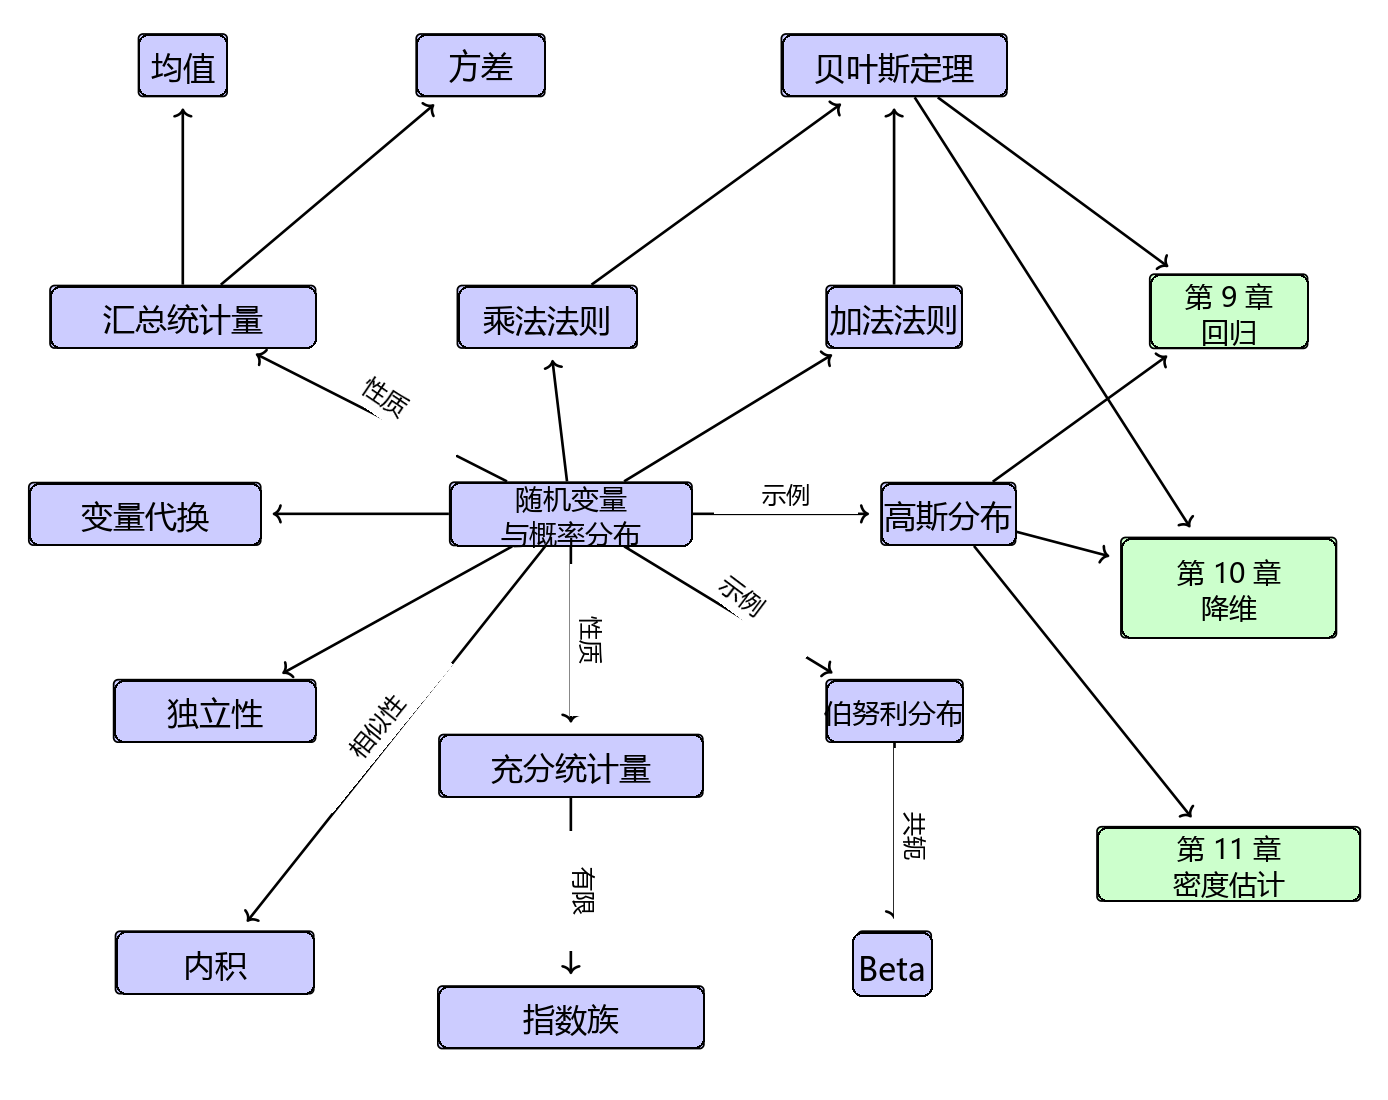
\includegraphics[width=0.92\textwidth,keepaspectratio]{docs/images/Figure6.1.png}
\caption*{\refstepcounter{figcounter}\label{fig:6-1}图~\thefigcounter 本章所描述的与随机变量和概率分布相关的概念思维导图。}
\end{figure}


\section*{6.1 概率空间的构造}
\addcontentsline{toc}{section}{6.1 概率空间的构造}
\label{sec:6.1}

概率论旨在定义一种数学结构来描述实验的随机结果。例如，在抛单枚硬币时，我们无法预先确定结果，但通过进行大量的投掷试验，我们可以观察到平均结果中的统计规律性。利用这种概率数学结构，我们的目标是执行自动化推理；从这个意义上讲，概率论推广了逻辑推理（Jaynes, 2003）。

\section*{6.1.1 哲学层面的思考}
\addcontentsline{toc}{subsection}{6.1.1 哲学层面的思考}

在构建自动化推理系统时，经典布尔逻辑并不允许我们表达某些形式的似真推理（plausible reasoning）。考虑如下场景：我们观察到 $ A $ 为假，会发现 $ B $ 变得不那么可信，尽管从经典逻辑中无法得出明确结论；反之，若观察到 $ B $ 为真，似乎 $ A $ 变得更加可信。我们在日常生活中时刻都在使用这种推理形式。例如，我们正在等待一位朋友，并考虑三种可能性：$ H_1 $，她准时到达；$ H_2 $，她因交通拥堵而延误；$ H_3 $，她被外星人劫持。当我们观察到朋友迟到了，从逻辑上必然排除 $ H_1 $；我们通常倾向于认为 $ H_2 $ 的可能性增大，尽管在纯逻辑上并没有必然要求我们这么做；最后，我们可能认为 $ H_3 $ 并非完全不可能，但仍然认为它极不可能发生。我们如何得出 $ H_2 $ 是最合理的解释？

从这个视角来看，“为了进行似真推理，有必要将离散的‘真’与‘假’真值扩展为连续的似真度”（Jaynes, 2003）。因此，概率论可以被视为布尔逻辑的一种推广。在机器学习语境中，它常被用于形式化自动化推理系统的设计。关于概率论如何作为推理系统基石的更深入讨论，可参阅 Pearl (1988)。

概率论的哲学基础以及它应如何与我们所认为的“真”（逻辑意义上的真）建立联系，由 Cox 进行了系统研究（Jaynes, 2003）。另一种理解方式是：如果我们对常识进行精确的数学刻画，最终便会构建出概率。E. T. Jaynes（1922–1998）指出了所有似真度必须满足的三个数学准则：

\begin{enumerate}
\item 似真度用实数表示。
\item 这些实数值必须基于常识法则。
\item 由此产生的推理必须具备一致性（consistency），包含以下三重含义：
\begin{itemize}
\item \emph{一致性或无矛盾性（Consistency or non-contradiction）} ：当可以通过不同途径得出同一结论时，在所有情况下求得的似真度必须相同。
\item \emph{诚实性（Honesty）} ：必须充分考虑所有可用数据。
\item \emph{可复现性（Reproducibility）} ：如果我们对两个问题的认知状态相同，则必须为它们赋予相同的似真度。
\end{itemize}
\end{enumerate}

Cox–Jaynes 定理证明了这些似真度准则足以定义适用于似真度 $ p $ 的普遍数学法则（在任意单调函数变换的意义下）。至关重要的是，这些法则正是概率的运算准则。

\emph{备注} 。在机器学习与统计学中，对概率存在两种主流解释：贝叶斯学派（Bayesian）解释与频率学派（frequentist）解释（Bishop, 2006; Efron and Hastie, 2016）。贝叶斯解释使用概率来量化用户对某事件的不确定程度，有时被称为“主观概率”或“置信度（degree of belief）”。频率学派解释则考虑感兴趣事件的发生次数占总试验次数的相对频率，事件的概率被定义为当数据量趋于无穷大时该事件相对频率的极限。♦

一些关于概率模型的机器学习文献在使用符号和术语时较为随意，容易引起混淆，本书也不例外。多个不同的概念往往都被统称为“概率分布”，读者通常需要根据上下文理清其确切含义。理清概率分布的一个诀窍是检验我们建模的对象是类别型对象（离散随机变量）还是连续型对象（连续随机变量）。我们在机器学习中处理的问题类型与所考虑的是类别模型还是连续模型紧密相关。

\medskip\hrule\medskip

\section*{6.1.2 概率与随机变量}
\addcontentsline{toc}{subsection}{6.1.2 概率与随机变量}

在讨论概率时，有三个截然不同但常被混淆的概念：

\begin{enumerate}
\item \emph{概率空间（probability space）} ：使我们能够对概率的概念进行量化。但在实际中我们大多不直接在这个基本概率空间中操作；
\item \emph{随机变量（random variable）} ：将概率转移到一个更方便（通常是数值型）的空间；
\item 与随机变量相关联的 \emph{分布（distribution）} 或 \emph{概率律（law）} 。
\end{enumerate}

我们将在本小节介绍前两个概念，并在第 6.2 节展开讨论第三个概念。

现代概率论建立在柯尔莫哥洛夫提出的一套公理基础之上（Grinstead and Snell, 1997; Jaynes, 2003），引入了样本空间、事件空间和概率测度三个核心概念。概率空间对具有随机结果的现实世界过程（称为实验）进行建模：

\begin{itemize}
\item \textbf{样本空间 $ \Omega $（The sample space $ \Omega $）}： 实验所有可能结果的集合，通常记为 $ \Omega $。例如，连续两次投掷硬币的样本空间为 $ \{hh, tt, ht, th\} $，其中 $ h $ 表示正面朝上（heads），$ t $ 表示反面朝上（tails）。
\item \textbf{事件空间 $ \mathcal{A} $（The event space $ \mathcal{A} $）}： 实验潜在结果的空间。样本空间 $ \Omega $ 的一个子集 $ A $ 属于事件空间 $ \mathcal{A} $，如果实验结束时我们可以观察到特定结果 $ \omega \in \Omega $ 是否落在 $ A $ 中。事件空间 $ \mathcal{A} $ 是通过考察 $ \Omega $ 的子集族构成的；对于离散概率分布（第 6.2.1 节），$ \mathcal{A} $ 通常是 $ \Omega $ 的幂集。
\item \textbf{概率 $ P $（The probability $ P $）}： 对于每个事件 $ A \in \mathcal{A} $，我们赋予一个数值 $ P(A) $，用于度量该事件发生的可信程度或概率。$ P(A) $ 称为事件 $ A $ 的 \emph{概率（probability）} 。
\end{itemize}

单个事件的概率必须位于区间 $ [0, 1] $ 内，且样本空间 $ \Omega $ 中所有结果的总概率必须为 1，即 $ P(\Omega) = 1 $。

给定概率空间 $ (\Omega, \mathcal{A}, P) $，我们希望用它来建模某些现实世界现象。在机器学习中，我们通常避免显式提及概率空间，而是直接关注感兴趣的量上的概率，我们将其空间记为 $ \mathcal{T} $。在本书中，我们称 $ \mathcal{T} $ 为 \emph{目标空间（target space）} ，并称 $ \mathcal{T} $ 中的元素为 \emph{状态（states）} 。我们引入一个函数：

\begin{equation*}
X : \Omega \to \mathcal{T}
\end{equation*}

它接收 $ \Omega $ 中的一个元素（实验结果），并返回一个特定的感兴趣量 $ x $（$ \mathcal{T} $ 中的一个值）。这种从 $ \Omega $ 到 $ \mathcal{T} $ 的映射称为 \emph{随机变量（random variable）} 。

\emph{提示} ：“随机变量”这一名称是许多误解的根源，因为它既不是随机的，也不是一个变量，而是一个确定性的函数。

例如，在掷两枚硬币并统计正面朝上次数的实验中，随机变量 $ X $ 映射到三个可能的结果：$ X(hh) = 2, X(ht) = 1, X(th) = 1, X(tt) = 0 $。在这个具体情形中，目标空间 $ \mathcal{T} = \{0, 1, 2\} $，我们感兴趣的正是 $ \mathcal{T} $ 中各元素的概率。对于有限样本空间 $ \Omega $ 和有限目标空间 $ \mathcal{T} $，对应于随机变量的函数本质上就是一个查找表。对于任意子集 $ S \subseteq \mathcal{T} $，我们将 $ P_X(S) \in [0, 1] $ 关联到对应于随机变量 $ X $ 的特定事件上。

\emph{备注} 。样本空间 $ \Omega $ 在不同教材中有不同的称呼。另一个常见名称是“状态空间（state space）”（Jacod and Protter, 2004），但状态空间有时专门用于指代动力系统中的状态。描述 $ \Omega $ 的其他名称还包括“样本描述空间”、“可能性空间”和“事件空间”。♦

\begin{notebox}
\textbf{例 6.1}
\end{notebox}

\begin{notebox}
考虑一个统计实验：从一个装有硬币的袋子中（有放回地）抽取两枚硬币。袋中有来自美国的硬币（记作 \$）和来自英国的硬币（记作 £）。因为抽取两次，总共有四种可能结果。该实验的状态空间或样本空间为 \$ \textbackslash\{\}Omega = \textbackslash\{\}\{(\$, \$), (\$, £), (£, \$), (£, £)\textbackslash\{\}\} \$。假定袋中硬币的构成使得单次抽取得到 \$ 的概率为 0.3。
\end{notebox}

\begin{notebox}
我们感兴趣的事件是重复抽取中获得 \$ 的总次数。我们定义随机变量 $ X : \Omega \to \mathcal{T} $ 表示从袋中抽出 \$ 的次数。由样本空间可知抽得 \$ 的次数可能为 0、1 或 2，因此 $ \mathcal{T} = \{0, 1, 2\} $。随机变量 $ X $（查找表）可表示为：

\begin{equation}
X((\$, \$)) = 2
\tag{6.1}\label{eq:6-1}
\end{equation}

\begin{equation}
X((\$, £)) = 1
\tag{6.2}\label{eq:6-2}
\end{equation}

\begin{equation}
X((£, \$)) = 1
\tag{6.3}\label{eq:6-3}
\end{equation}

\begin{equation}
X((£, £)) = 0
\tag{6.4}\label{eq:6-4}
\end{equation}

由于我们在抽取第二枚硬币前放回了第一枚，两次抽取相互独立（见第 6.4.5 节）。注意到有两个实验结果对应于只抽得一次 \$ 的同一个事件。因此，$ X $ 的 \emph{概率质量函数（probability mass function）} 给出为：

\begin{equation}
P(X = 2) = P((\$, \$)) = P(\$) \cdot P(\$) = 0.3 \cdot 0.3 = 0.09
\tag{6.5}\label{eq:6-5}
\end{equation}

\begin{equation}
P(X = 1) = P((\$, £) \cup (£, \$)) = P((\$, £)) + P((£, \$)) = 0.3 \cdot (1 - 0.3) + (1 - 0.3) \cdot 0.3 = 0.42
\tag{6.6}\label{eq:6-6}
\end{equation}

\begin{equation}
P(X = 0) = P((£, £)) = P(£) \cdot P(£) = (1 - 0.3) \cdot (1 - 0.3) = 0.49
\tag{6.7}\label{eq:6-7}
\end{equation}
\end{notebox}

在上述计算中，我们将两个不同的概念等同了起来：$ X $ 输出的概率与 $ \Omega $ 中样本的概率。例如在式~\eqref{eq:6-7} 中，我们写道 $ P(X = 0) = P((£, £)) $。考虑随机变量 $ X : \Omega \to \mathcal{T} $ 以及子集 $ S \subseteq \mathcal{T} $。设 $ X^{-1}(S) $ 为 $ S $ 在 $ X $ 下的 \emph{原像（pre-image）} ，即 $ \Omega $ 中在 $ X $ 作用下映射到 $ S $ 的元素集合：$ \{\omega \in \Omega : X(\omega) \in S\} $。理解概率从 $ \Omega $ 中的事件经由随机变量 $ X $ 转移的一种方式，是将其与 $ S $ 原像的概率相关联（Jacod and Protter, 2004）。对于 $ S \subseteq \mathcal{T} $，我们采用如下记号：

\begin{equation}
P_X(S) = P(X \in S) = P(X^{-1}(S)) = P(\{\omega \in \Omega : X(\omega) \in S\})
\tag{6.8}\label{eq:6-8}
\end{equation}

式~\eqref{eq:6-8} 的左侧是我们感兴趣的可能结果集合（例如 \$ 的个数等于 1）的概率；右侧表明这是 $ \Omega $ 中具备该性质的状态集合（例如 \$£, £\$）的概率。我们称随机变量 $ X $ 服从特定的概率分布 $ P_X $，该分布定义了事件与随机变量结果概率之间的映射关系。换言之，函数 $ P_X $（或等价地 $ P \circ X^{-1} $）是随机变量 $ X $ 的 \emph{概率律（law）} 或 \emph{概率分布（distribution）} 。

\emph{备注} 。目标空间（即随机变量 $ X $ 的值域 $ \mathcal{T} $）用于指明概率空间的类型。当 $ \mathcal{T} $ 是有限集或可数无限集时，称为 \emph{离散随机变量（discrete random variable）} （第 6.2.1 节）。对于 \emph{连续随机变量（continuous random variable）} （第 6.2.2 节），我们通常只考虑 $ \mathcal{T} = \mathbb{R} $ 或 $ \mathcal{T} = \mathbb{R}^D $。♦

\medskip\hrule\medskip

\section*{6.1.3 统计学}
\addcontentsline{toc}{subsection}{6.1.3 统计学}

概率论与统计学常常相伴出现，但它们关注不确定性的不同侧面。对比它们的一种方式是考察它们所处理的问题类型：

\begin{itemize}
\item 在 \textbf{概率论} 中，我们考虑某个过程的模型，其中潜在的不确定性由随机变量刻画，我们利用概率法则来推导将会发生什么；
\item 在 \textbf{统计学} 中，我们观察到某些已经发生的事实，并试图推断能够解释这些观测结果的底层过程。
\end{itemize}

从这个意义上讲，机器学习与统计学非常接近，其目标都是构建能够充分表征生成数据过程的模型。我们可以使用概率法则来为某些数据获得“最佳拟合”的模型。

机器学习系统的另一个核心方面是我们关注 \emph{泛化误差（generalization error）} （参见第 8 章）。这意味着我们关注系统在未来观测到的新样本上的表现，而这些样本与我们迄今见过的样本并不完全相同。对未来表现的分析依赖于概率论与统计学，相关进阶讨论可参阅 Boucheron et al. (2013) 以及 Shalev-Shwartz and Ben-David (2014)。

\section*{6.2 离散与连续概率}
\addcontentsline{toc}{section}{6.2 离散与连续概率}
\label{sec:6.2}

现在让我们将注意力聚焦在如何描述事件的概率上。根据目标空间是离散的还是连续的，指代概率分布的自然方式有所不同：

\begin{itemize}
\item 当目标空间 $ \mathcal{T} $ 是离散的时，我们可以明确指定随机变量 $ X $ 取特定值 $ x \in \mathcal{T} $ 的概率，记为 $ P(X = x) $。对于离散随机变量 $ X $，表达式 $ P(X = x) $ 称为 \emph{概率质量函数（probability mass function, pmf）} 。
\item 当目标空间 $ \mathcal{T} $ 是连续的时（例如实数线 $ \mathbb{R} $），更自然的方式是指定随机变量 $ X $ 落在某个区间内的概率，对于 $ a < b $ 记为 $ P(a \leqslant X \leqslant b) $。按照惯例，我们通常指定随机变量 $ X $ 小于或等于特定值 $ x $ 的概率，记为 $ P(X \leqslant x) $。对于连续随机变量 $ X $，表达式 $ P(X \leqslant x) $ 称为 \emph{累积分布函数（cumulative distribution function, cdf）} 。
\end{itemize}

\emph{备注} 。我们使用短语 \emph{单变量分布（univariate distribution）} 来指代单个随机变量的分布（其状态用非粗体 $ x $ 表示）；使用 \emph{多元分布（multivariate distribution）} 指代多个随机变量的联合分布，通常考虑随机变量构成的向量（其状态用粗体 $ \boldsymbol{x} $ 表示）。♦

\medskip\hrule\medskip

\section*{6.2.1 离散概率}
\addcontentsline{toc}{subsection}{6.2.1 离散概率}

当目标空间是离散的时，我们可以将多个随机变量的联合概率分布想象为填满一个多维数值数组。图~\ref{fig:6-2} 给出了一个示例。联合概率的目标空间是各个随机变量目标空间的笛卡尔积。我们定义联合概率为两个值联合出现的概率：

\begin{equation}
P(X = x_i, Y = y_j) = \frac{n_{ij}}{N}
\tag{6.9}\label{eq:6-9}
\end{equation}

其中 $ n_{ij} $ 是处于状态 $ x_i $ 和 $ y_j $ 的事件数，而 $ N $ 是事件总数。联合概率即为两个事件交集的概率，即 $ P(X = x_i, Y = y_j) = P(X = x_i \cap Y = y_j) $。


\begin{figure}[H]
\centering
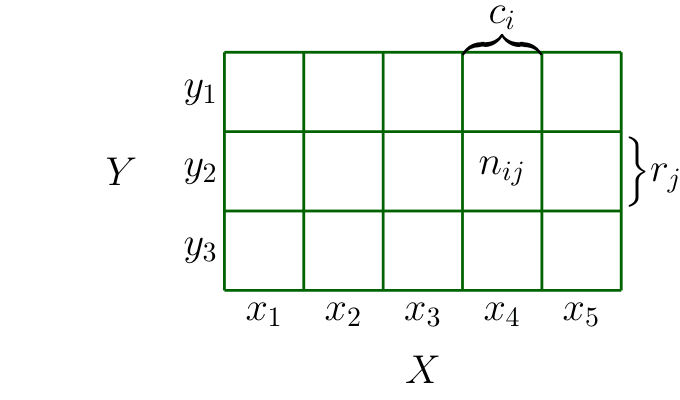
\includegraphics[width=0.92\textwidth,keepaspectratio]{docs/images/Figure6.2.png}
\caption*{\refstepcounter{figcounter}\label{fig:6-2}图~\thefigcounter 随机变量 X 和 Y 的离散二元概率质量函数的可视化。}
\end{figure}


图~\ref{fig:6-2} 说明了离散概率分布的概率质量函数（pmf）。对于两个随机变量 $ X $ 和 $ Y $，$ X = x $ 且 $ Y = y $ 的概率常简记为 $ p(x, y) $，称为 \emph{联合概率（joint probability）} 。我们可以将概率视为以状态 $ x $ 和 $ y $ 为自变量并返回实数的函数，这也是我们写作 $ p(x, y) $ 的原因。无论随机变量 $ Y $ 取何值，$ X $ 取值 $ x $ 的 \emph{边缘概率（marginal probability）} 简记为 $ p(x) $。我们写作 $ X \sim p(x) $ 来表示随机变量 $ X $ 服从分布 $ p(x) $。如果我们仅考虑 $ X = x $ 的样本，那么其中 $ Y = y $ 所占的比例（ \emph{条件概率（conditional probability）} ）简记为 $ p(y \mid x) $。

\begin{notebox}
\textbf{例 6.2}
\end{notebox}

\begin{notebox}
考虑两个随机变量 $ X $ 和 $ Y $，其中 $ X $ 有 5 个可能状态，$ Y $ 有 3 个可能状态，如图~\ref{fig:6-2} 所示。我们用 $ n_{ij} $ 表示处于状态 $ X = x_i $ 且 $ Y = y_j $ 的事件数，用 $ N $ 表示事件总数。数值 $ c_i $ 是第 $ i $ 列各频数之和，即 $ c_i = \sum_{j=1}^3 n_{ij} $；类似地，$ r_j $ 是行和，即 $ r_j = \sum_{i=1}^5 n_{ij} $。利用这些定义，我们可以紧凑地表示 $ X $ 和 $ Y $ 的分布。
\end{notebox}

\begin{notebox}
每个随机变量的概率分布（即边缘概率）可以视为对某一行或某一列求和：

\begin{equation}
P(X = x_i) = \frac{c_i}{N} = \frac{\sum_{j=1}^3 n_{ij}}{N}
\tag{6.10}\label{eq:6-10}
\end{equation}

\begin{equation}
P(Y = y_j) = \frac{r_j}{N} = \frac{\sum_{i=1}^5 n_{ij}}{N}
\tag{6.11}\label{eq:6-11}
\end{equation}

其中 $ c_i $ 和 $ r_j $ 分别是概率表格的第 $ i $ 列和第 $ j $ 行的和。对于具有有限个事件的离散随机变量，所有概率之和为 1：

\begin{equation}
\sum_{i=1}^5 P(X = x_i) = 1 \quad \textcn{且} \quad \sum_{j=1}^3 P(Y = y_j) = 1
\tag{6.12}\label{eq:6-12}
\end{equation}

条件概率是特定单元格在某一行或某一列中所占的比例。例如，给定 $ X $ 时 $ Y $ 的条件概率为：

\begin{equation}
P(Y = y_j \mid X = x_i) = \frac{n_{ij}}{c_i}
\tag{6.13}\label{eq:6-13}
\end{equation}

给定 $ Y $ 时 $ X $ 的条件概率为：

\begin{equation}
P(X = x_i \mid Y = y_j) = \frac{n_{ij}}{r_j}
\tag{6.14}\label{eq:6-14}
\end{equation}
\end{notebox}

在机器学习中，我们使用离散概率分布对类别变量（categorical variables，即取有限个无序值的变量）进行建模。它们可以是类别特征（如预测薪资时所用的大学专业），也可以是类别标签（如手写识别中的字母）。离散分布也常用于构建混合了有限个连续分布的概率模型（第 11 章）。

\medskip\hrule\medskip

\section*{6.2.2 连续概率}
\addcontentsline{toc}{subsection}{6.2.2 连续概率}

在本节中，我们考虑实值随机变量，即目标空间为实数线 $ \mathbb{R} $ 上的区间。在本书中，我们可以大致像处理有限状态离散空间一样对实值随机变量执行操作。但在两种情况下这种简化不够严谨：当重复某事无限次时，以及当我们希望从一个区间中随机抽取一个点时。第一种情形出现在讨论机器学习的泛化误差时（第 8 章）；第二种情形出现在讨论连续分布（如高斯分布，第 6.5 节）时。

\emph{备注} 。在连续空间中存在两个与直觉相悖的技术细节。首先，所有子集的集合（第 6.1 节中用于定义事件空间 $ \mathcal{A} $ 的幂集）性质不够良好，必须限制 $ \mathcal{A} $ 在补集、交集和并集运算下保持封闭。其次，集合的“大小”（测度，measure）在连续空间中不能简单通过计数得到。例如离散集合的势（元素个数）、$ \mathbb{R} $ 中区间的长度以及 $ \mathbb{R}^d $ 中区域的体积都是测度的例子。在集合运算下封闭且具有拓扑结构的集合系称为 \emph{Borel $ \sigma $-代数（Borel $ \sigma $-algebra）} 。在本书中，我们考虑实值随机变量及其对应的 Borel $ \sigma $-代数，并将取值于 $ \mathbb{R}^D $ 的随机变量视为实值随机变量构成的向量。♦

\textbf{定义 6.1}（概率密度函数）。如果函数 $ f : \mathbb{R}^D \to \mathbb{R} $ 满足：

\begin{enumerate}
\item $ \forall \boldsymbol{x} \in \mathbb{R}^D : f(\boldsymbol{x}) \geqslant 0 $
\item 其积分存在且：
\end{enumerate}

\begin{equation}
\int_{\mathbb{R}^D} f(\boldsymbol{x})\,\mathrm{d}\boldsymbol{x} = 1
\tag{6.15}\label{eq:6-15}
\end{equation}

则称 $ f $ 为 \emph{概率密度函数（probability density function, pdf）} 。

对于离散随机变量的概率质量函数（pmf），式~\eqref{eq:6-15} 中的积分替换为求和 (6.12)。

概率密度函数是任何非负且在全空间积分为 1 的函数 $ f $。我们将随机变量 $ X $ 与该函数 $ f $ 通过如下方式相关联：

\begin{equation}
P(a \leqslant X \leqslant b) = \int_a^b f(x)\,\mathrm{d}x
\tag{6.16}\label{eq:6-16}
\end{equation}

其中 $ a, b \in \mathbb{R} $ 且 $ x \in \mathbb{R} $ 是连续随机变量 $ X $ 的可能结果。状态 $ \boldsymbol{x} \in \mathbb{R}^D $ 可类似地通过考虑向量形式给出。这种关联 (6.16) 称为随机变量 $ X $ 的 \emph{概率律（law）} 或 \emph{分布（distribution）} 。

\emph{备注} 。与离散随机变量形成鲜明对比的是，连续随机变量 $ X $ 取某一具体单点数值的概率恒为零：$ P(X = x) = 0 $。这相当于在式~\eqref{eq:6-16} 中指定区间端点 $ a = b $。单点集是测度为零的集合。♦

\textbf{定义 6.2}（累积分布函数）。状态为 $ \boldsymbol{x} \in \mathbb{R}^D $ 的多元实值随机变量 $ \boldsymbol{X} $ 的 \emph{累积分布函数（cumulative distribution function, cdf）} 定义为：

\begin{equation}
F_{\boldsymbol{X}}(\boldsymbol{x}) = P(X_1 \leqslant x_1, \ldots, X_D \leqslant x_D)
\tag{6.17}\label{eq:6-17}
\end{equation}

其中 $ \boldsymbol{X} = [X_1, \ldots, X_D]^\top $，$ \boldsymbol{x} = [x_1, \ldots, x_D]^\top $，等号右侧表示随机变量 $ X_i $ 取小于或等于 $ x_i $ 的值的概率。

累积分布函数也可以表示为概率密度函数 $ f(\boldsymbol{x}) $ 的多重积分：

\begin{equation}
F_{\boldsymbol{X}}(\boldsymbol{x}) = \int_{-\infty}^{x_1} \cdots \int_{-\infty}^{x_D} f(z_1, \ldots, z_D)\,\mathrm{d}z_1 \cdots \mathrm{d}z_D
\tag{6.18}\label{eq:6-18}
\end{equation}

\emph{提示} ：存在不具备对应概率密度函数的累积分布函数。

\emph{备注} 。我们再次强调，在讨论分布时实际上包含两个截然不同的概念：其一是 pdf（记为 $ f(x) $），它是一个积分为 1 的非负函数；其二是随机变量 $ X $ 的概率律，即随机变量 $ X $ 与 pdf $ f(x) $ 之间的映射关联。♦

\medskip\hrule\medskip

\section*{6.2.3 离散与连续分布的对比}
\addcontentsline{toc}{subsection}{6.2.3 离散与连续分布的对比}

回顾第 6.1.2 节，概率是非负的，且总概率之和为 1。对于离散随机变量（见式~\eqref{eq:6-12}），这意味着每个状态的概率必须位于区间 $ [0, 1] $ 内。然而，对于连续随机变量，归一化条件 (6.15) 并不意味着密度函数的值在所有点都小于或等于 1。我们在图~\ref{fig:6-3} 中使用离散与连续均匀分布对此进行说明。


\begin{figure}[H]
\centering
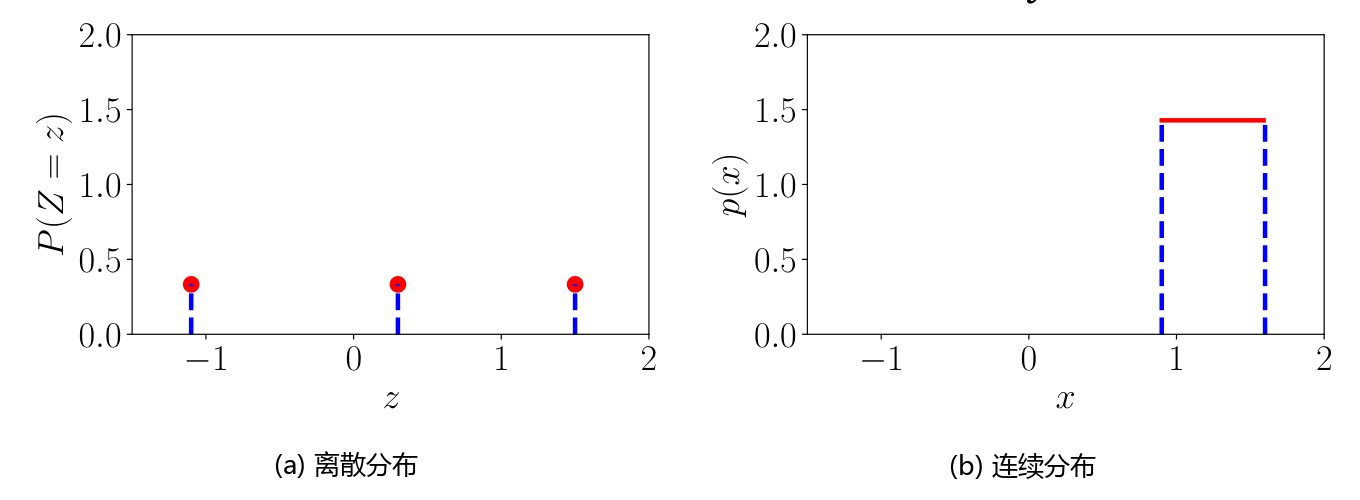
\includegraphics[width=0.92\textwidth,keepaspectratio]{docs/images/Figure6.3.png}
\caption*{\refstepcounter{figcounter}\label{fig:6-3}图~\thefigcounter (a) 离散与 (b) 连续均匀分布的示例。}
\end{figure}


\begin{notebox}
\textbf{例 6.3}
\end{notebox}

\begin{notebox}
我们考虑两个均匀分布的示例，其中每个状态发生的可能性均等。
\end{notebox}

\begin{notebox}
设 $ Z $ 为具有三个状态 $ \{z = -1.1, z = 0.3, z = 1.5\} $ 的离散均匀随机变量。其概率质量函数可表示为概率数值表：
\end{notebox}

\begin{notebox}
\begin{longtable}{>{\raggedright\arraybackslash}p{\dimexpr(\textwidth-24pt)/2\relax} >{\raggedright\arraybackslash}p{\dimexpr(\textwidth-24pt)/2\relax}}
\hline
\textbf{$z$} & \textbf{$P(Z = z)$} \\ \hline
\endhead
$-1.1$ & $\frac{1}{3}$ \\ \hline
$0.3$ & $\frac{1}{3}$ \\ \hline
$1.5$ & $\frac{1}{3}$ \\ \hline
\end{longtable}
\end{notebox}

\begin{notebox}
或者，我们可以将其表示为一个图（图~\ref{fig:6-3}(a)），其中状态位于横轴，纵轴表示特定状态的概率。
\end{notebox}

\begin{notebox}
设 $ X $ 为在区间 $ 0.9 \leqslant X \leqslant 1.6 $ 内取值的连续随机变量，如图~\ref{fig:6-3}(b) 所示。注意到概率密度的高度大于 1（高度为 $ \frac{1}{1.6 - 0.9} = \frac{1}{0.7} \approx 1.43 > 1 $）。然而，整个密度函数的积分必须为 1：

\begin{equation}
\int_{0.9}^{1.6} p(x)\,\mathrm{d}x = 1
\tag{6.19}\label{eq:6-19}
\end{equation}
\end{notebox}

\emph{备注} 。关于离散概率分布还有一个细微之处：状态 $ z_1, \ldots, z_d $ 原则上不需要具备任何序结构（例如 $ z_1 = \textcn{红}, z_2 = \textcn{绿}, z_3 = \textcn{蓝} $）。但在许多机器学习应用中，离散状态通常取数值（例如 $ z_1 = -1.1, z_2 = 0.3, z_3 = 1.5 $），此时可以定义顺序 $ z_1 < z_2 < z_3 $。取数值的离散状态尤其实用，因为我们经常需要计算随机变量的期望值（第 6.4.1 节）。♦

机器学习文献中的符号常常掩盖了样本空间 $ \Omega $、目标空间 $ \mathcal{T} $ 与随机变量 $ X $ 之间的区别。对于随机变量 $ X $ 的可能结果值 $ x \in \mathcal{T} $，$ p(x) $ 表示随机变量 $ X $ 产生结果 $ x $ 的概率。对于离散随机变量，这写作 $ P(X = x) $，称为概率质量函数（通常直接称为“分布”）。对于连续变量，$ p(x) $ 称为概率密度函数（常简称为“密度”）。更为混淆的是，累积分布函数 $ P(X \leqslant x) $ 也常被称为“分布”。我们在表 6.1 中总结了这些术语规范。

\begin{longtable}{>{\raggedright\arraybackslash}p{\dimexpr(\textwidth-36pt)/3\relax} >{\raggedright\arraybackslash}p{\dimexpr(\textwidth-36pt)/3\relax} >{\raggedright\arraybackslash}p{\dimexpr(\textwidth-36pt)/3\relax}}
\hline
\textbf{类型} & \textbf{“单点概率”} & \textbf{“区间概率”} \\ \hline
\endhead
\textbf{离散} & $P(X = x)$ \newline  概率质量函数（pmf） & 不适用 \\ \hline
\textbf{连续} & $p(x)$ \newline  概率密度函数（pdf） & $P(X \leqslant x)$ \newline  累积分布函数（cdf） \\ \hline
\end{longtable}

\emph{备注} 。在本书中，尽管在严格数学上并不严谨，我们仍将跟随绝大多数机器学习文献的惯例，不仅对离散概率质量函数，而且对连续概率密度函数也使用“概率分布”这一统称，读者可结合上下文轻松分辨其确切含义。♦

\section*{6.3 加法法则、乘法法则与贝叶斯定理}
\addcontentsline{toc}{section}{6.3 加法法则、乘法法则与贝叶斯定理}
\label{sec:6.3}

我们可以将概率论视为逻辑推理的一种扩展。正如我们在第 6.1.1 节中所讨论的，这里介绍的概率法则很自然地源于对基本准则的满足（Jaynes, 2003，第 2 章）。概率建模（第 8.4 节）为设计机器学习方法提供了原则性的理论基石。一旦我们定义了与数据和问题的不确定性相对应的概率分布（第 6.2 节），就会发现其实只有两条基本法则：加法法则与乘法法则。

回顾式~\eqref{eq:6-9}，$ p(x, y) $ 是两个随机变量 $ X, Y $ 的联合分布。分布 $ p(x) $ 和 $ p(y) $ 是对应的边缘分布，而 $ p(y \mid x) $ 是给定 $ x $ 时 $ y $ 的条件分布。基于第 6.2 节中给出的离散和连续随机变量的边缘概率与条件概率的定义，我们现在可以给出概率论中的两条基本法则。这两条法则自然地源于我们在第 6.1.1 节中讨论的准则（Jaynes, 2003）。

第一条法则是 \emph{加法法则（sum rule）} ，表述为：

\begin{equation}
p(x) =
\begin{cases}
\sum_{y \in \mathcal{Y}} p(x, y) & \textcn{若 } y \textcn{ 是离散的} \\
\int_{\mathcal{Y}} p(x, y)\,\mathrm{d}y & \textcn{若 } y \textcn{ 是连续的}
\end{cases}
\tag{6.20}\label{eq:6-20}
\end{equation}

其中 $ \mathcal{Y} $ 是随机变量 $ Y $ 的目标空间状态集。这意味着我们对随机变量 $ Y $ 的所有状态集 $ y $ 进行求和（或积分消去）。加法法则也称为 \emph{边际化性质（marginalization property）} 。

加法法则将联合分布与边缘分布联系起来。一般而言，当联合分布包含多于两个随机变量时，加法法则可以应用于随机变量的任意子集，从而得到可能包含多个随机变量的边缘分布。具体来说，若 $ \boldsymbol{x} = [x_1, \ldots, x_D]^\top $，我们通过反复应用加法法则，对除 $ x_i $ 之外的所有随机变量进行积分/求和消去，即可得到边缘分布：

\begin{equation}
p(x_i) = \int p(x_1, \ldots, x_D)\,\mathrm{d}\boldsymbol{x}_{\backslash i}
\tag{6.21}\label{eq:6-21}
\end{equation}

其中 $ \backslash i $ 表示“除 $ i $ 之外的所有变量”。

\emph{备注} 。概率建模中的许多计算挑战都源于加法法则的应用。当存在大量变量，或者离散变量具有大量状态时，加法法则归结为执行高维求和或高维积分。从计算角度来看，执行高维求和或积分通常是极其困难的，因为目前尚不存在已知的多项式时间算法能够精确计算它们。♦

第二条法则称为 \emph{乘法法则（product rule）} ，它通过以下方式将联合分布与条件分布联系起来：

\begin{equation}
p(x, y) = p(y \mid x) p(x)
\tag{6.22}\label{eq:6-22}
\end{equation}

乘法法则可以解释为：两个随机变量的任意联合分布都可以分解（表示为乘积）为另外两个分布。这两个因子分别是第一个随机变量的边缘分布 $ p(x) $，以及给定第一个随机变量时第二个随机变量的条件分布 $ p(y \mid x) $。由于在 $ p(x, y) $ 中随机变量的排列顺序是任意的，乘法法则同样意味着 $ p(x, y) = p(x \mid y) p(y) $。严格来说，式~\eqref{eq:6-22} 是针对离散随机变量的概率质量函数表述的；对于连续随机变量，乘法法则则是针对概率密度函数表述的（第 6.2.3 节）。

在机器学习和贝叶斯统计中，我们经常关注在已经观测到某些随机变量的情况下，对未观测到的（潜在）随机变量进行推断。假设我们对未观测到的随机变量 $ x $ 具有某种先验知识 $ p(x) $，并且已知 $ x $ 与我们能够观测到的第二个随机变量 $ y $ 之间的某种关系 $ p(y \mid x) $。如果观测到了 $ y $，我们就可以利用贝叶斯定理，根据 $ y $ 的观测值推导出关于 $ x $ 的结论。 \emph{贝叶斯定理（Bayes' theorem，亦称贝叶斯法则 Bayes' rule 或贝叶斯定律 Bayes' law）} ：

\begin{equation}
\underbrace{p(x \mid y)}_{\textcn{后验}} = \frac{\overbrace{p(y \mid x)}^{\textcn{似然}} \overbrace{p(x)}^{\textcn{先验}}}{\underbrace{p(y)}_{\textcn{证据}}}
\tag{6.23}\label{eq:6-23}
\end{equation}

是式~\eqref{eq:6-22} 中乘法法则的直接推论，因为：

\begin{equation}
p(x, y) = p(x \mid y) p(y)
\tag{6.24}\label{eq:6-24}
\end{equation}

且

\begin{equation}
p(x, y) = p(y \mid x) p(x)
\tag{6.25}\label{eq:6-25}
\end{equation}

从而有：

\begin{equation}
p(x \mid y) p(y) = p(y \mid x) p(x) \iff p(x \mid y) = \frac{p(y \mid x) p(x)}{p(y)}
\tag{6.26}\label{eq:6-26}
\end{equation}

在式~\eqref{eq:6-23} 中，$ p(x) $ 是 \emph{先验（prior）} ，它概括了我们在观测到任何数据之前，对未观测到的（潜在）变量 $ x $ 的主观先验知识。我们可以选择任何对我们合理的先验，但关键是要确保在所有合理的 $ x $ 上先验都具有非零的概率密度（或概率质量），即使这些取值极少出现。

\emph{似然（likelihood）} $ p(y \mid x) $ 描述了 $ x $ 与 $ y $ 之间的关联方式；在离散概率分布的情况下，它是我们在已知潜在变量 $ x $ 时数据 $ y $ 出现的概率。似然有时也被称为“测量模型（measurement model）”。请注意，似然并不是关于 $ x $ 的分布，而只是关于 $ y $ 的分布。我们称 $ p(y \mid x) $ 为“（给定 $ y $ 时）$ x $ 的似然”或“给定 $ x $ 时 $ y $ 的概率”，但绝不能称其为 $ y $ 的似然（MacKay, 2003）。

\emph{后验（posterior）} $ p(x \mid y) $ 是贝叶斯统计中最核心的量，因为它恰好表达了我们所感兴趣的内容，即在观测到 $ y $ 之后我们所获得的关于 $ x $ 的知识。

量

\begin{equation}
p(y) := \int p(y \mid x) p(x)\,\mathrm{d}x = \mathbb{E}_X [p(y \mid x)]
\tag{6.27}\label{eq:6-27}
\end{equation}

称为 \emph{边际似然（marginal likelihood）} 或 \emph{证据（evidence）} 。式~\eqref{eq:6-27} 的右侧使用了我们在第 6.4.1 节中定义的期望算子。根据定义，边际似然对式~\eqref{eq:6-23} 的分子关于潜在变量 $ x $ 进行积分。因此，边际似然独立于 $ x $，它保证了后验 $ p(x \mid y) $ 是归一化的。边际似然也可以解释为期望似然，即对先验 $ p(x) $ 取期望。除了归一化后验之外，边际似然在贝叶斯模型选择中也起着重要作用，我们将在第 8.6 节中讨论这一点。由于式~\eqref{eq:8-44} 中的积分计算，证据往往很难求解。

贝叶斯定理 (6.23) 允许我们将似然所给出的 $ x $ 与 $ y $ 之间的关系进行反转。因此，贝叶斯定理有时也被称为 \emph{概率逆运算（probabilistic inverse）} 。我们将在第 8.4 节中进一步讨论贝叶斯定理。

\emph{备注} 。在贝叶斯统计中，后验分布是我们最关心的量，因为它囊括了来自先验和数据的所有可用信息。除了保留整个后验之外，我们也可以关注后验的某些统计量，例如后验的最大值（即最大后验），这将在第 8.3 节中进行讨论。然而，仅关注后验的某些统计量会导致信息损失。如果我们从更宏观的视角来考虑，后验可以应用于决策系统中，而拥有完整的后验分布对于做出抗扰动干扰的鲁棒决策极其有用。例如，在基于模型的强化学习语境下，Deisenroth et al. (2015) 表明，利用可能转移函数的完整后验分布可以实现非常快速（数据/样本高效）的学习，而仅关注后验最大值则会导致持续的失败。因此，拥有完整的后验对于下游任务而言大有裨益。在第 9 章中，我们将在线性回归的语境下继续这一讨论。♦

\section*{6.4 统计量与独立性}
\addcontentsline{toc}{section}{6.4 统计量与独立性}
\label{sec:6.4}

我们经常需要对一组随机变量进行概括汇总，并对成对的随机变量进行比较。随机变量的 \emph{统计量（statistic）} 是该随机变量的确定性函数。分布的 \emph{汇总统计量（summary statistics）} 为我们观察随机变量的行为提供了一个有用的视角，顾名思义，它提供了一组用于概括和刻画分布特征的数值。我们将介绍均值和方差这两个著名的汇总统计量。随后，我们将讨论比较一对随机变量的两种方法：第一，如何定义两个随机变量是独立的；第二，如何计算它们之间的内积。

\medskip\hrule\medskip

\section*{6.4.1 均值与协方差}
\addcontentsline{toc}{subsection}{6.4.1 均值与协方差}

均值和（协）方差通常用于描述概率分布的性质（期望值与分散程度）。我们将在第 6.6 节中看到一个非常有用的分布族（称为指数族），其中随机变量的统计量能够捕获所有可能的信息。

期望值的概念在机器学习中处于核心地位，概率本身的基本概念也可以从期望值推导出来（Whittle, 2000）。

\textbf{定义 6.3}（期望值）。单变量连续随机变量 $ X \sim p(x) $ 的函数 $ g : \mathbb{R} \to \mathbb{R} $ 的 \emph{期望值（expected value）} 给出为：

\begin{equation}
\mathbb{E}_X[g(x)] = \int_{\mathcal{X}} g(x)p(x)\,\mathrm{d}x
\tag{6.28}\label{eq:6-28}
\end{equation}

相应地，离散随机变量 $ X \sim p(x) $ 的函数 $ g $ 的期望值给出为：

\begin{equation}
\mathbb{E}_X[g(x)] = \sum_{x \in \mathcal{X}} g(x)p(x)
\tag{6.29}\label{eq:6-29}
\end{equation}

其中 $ \mathcal{X} $ 是随机变量 $ X $ 的可能结果集合（目标空间）。

在本节中，我们考虑取数值结果的离散随机变量。这可以通过观察到函数 $ g $ 以实数作为输入看出。随机变量函数的期望值有时被称为“无意识统计学家法则”（law of the unconscious statistician，Casella and Berger, 2002，第 2.2 节）。

\emph{备注} 。我们将多元随机变量 $ \boldsymbol{X} $ 视为单变量随机变量构成的有限向量 $ [X_1, \ldots, X_D]^\top $。对于多元随机变量，我们按元素逐项定义其期望值：

\begin{equation}
\mathbb{E}_{\boldsymbol{X}}[g(\boldsymbol{x})] = \begin{bmatrix} \mathbb{E}_{X_1}[g(x_1)] \\ \vdots \\ \mathbb{E}_{X_D}[g(x_D)] \end{bmatrix} \in \mathbb{R}^D
\tag{6.30}\label{eq:6-30}
\end{equation}

其中下标 $ \mathbb{E}_{X_d} $ 表示我们关于向量 $ \boldsymbol{x} $ 的第 $ d $ 个分量取期望值。♦

定义 6.3 定义了记号 $ \mathbb{E}_X $ 作为算子的含义，指示我们应当关于概率密度取积分（对于连续分布）或对所有状态求和（对于离散分布）。均值的定义（定义 6.4）是期望值的一个特例，只需选取 $ g $ 为恒等函数即可得到。

\textbf{定义 6.4}（均值）。状态为 $ \boldsymbol{x} \in \mathbb{R}^D $ 的随机变量 $ \boldsymbol{X} $ 的 \emph{均值（mean）} 是一种平均值，定义为：

\begin{equation}
\mathbb{E}_{\boldsymbol{X}}[\boldsymbol{x}] = \begin{bmatrix} \mathbb{E}_{X_1}[x_1] \\ \vdots \\ \mathbb{E}_{X_D}[x_D] \end{bmatrix} \in \mathbb{R}^D
\tag{6.31}\label{eq:6-31}
\end{equation}

其中对于 $ d = 1, \ldots, D $：

\begin{equation}
\mathbb{E}_{X_d}[x_d] :=
\begin{cases}
\int_{\mathcal{X}} x_d p(x_d)\,\mathrm{d}x_d & \textcn{若 } X \textcn{ 是连续随机变量} \\
\sum_{x_i \in \mathcal{X}} x_i p(x_d = x_i) & \textcn{若 } X \textcn{ 是离散随机变量}
\end{cases}
\tag{6.32}\label{eq:6-32}
\end{equation}

其中下标 $ d $ 表示 $ \boldsymbol{x} $ 的相应维度。积分和求和遍历随机变量 $ X $ 的目标空间状态集 $ \mathcal{X} $。

在一维情况下，还有另外两种直观的“平均值”概念，即中位数和众数。 \emph{中位数（median）} 是我们将所有数值排序后的“中间”值，即 50\% 的数值大于中位数，50\% 的数值小于中位数。这一概念可以通过考虑累积分布函数（定义 6.2）等于 0.5 处的值推广到连续变量。对于不对称或具有长尾的分布，中位数给出的典型值估计比均值更符合人类的直觉。此外，中位数对异常值的鲁棒性高于均值。将中位数推广到更高维度并非易事，因为在多于一个维度时并不存在显而易见的“排序”方式（Hallin et al., 2010; Kong and Mizera, 2012）。 \emph{众数（mode）} 是出现频率最高的值。对于离散随机变量，众数定义为具有最高出现频率的 $ x $ 值。对于连续随机变量，众数定义为概率密度 $ p(x) $ 的峰值。特定密度 $ p(x) $ 可能具有不止一个众数，而且在高维分布中可能存在数量极其庞大的众数。因此，寻找分布的所有众数在计算上极具挑战性。

\begin{notebox}
\textbf{例 6.4}
\end{notebox}

\begin{notebox}
考虑图~\ref{fig:6-4} 所示的二维分布：

\begin{equation}
\begin{adjustbox}{max width=\linewidth}
p(\boldsymbol{x}) = 0.4 \mathcal{N}\left(\boldsymbol{x} \;\middle|\; \begin{bmatrix} 10 \\ 2 \end{bmatrix}, \begin{bmatrix} 1 & 0 \\ 0 & 1 \end{bmatrix}\right) + 0.6 \mathcal{N}\left(\boldsymbol{x} \;\middle|\; \begin{bmatrix} 0 \\ 0 \end{bmatrix}, \begin{bmatrix} 8.4 & 2.0 \\ 2.0 & 1.7 \end{bmatrix}\right)
\end{adjustbox}
\tag{6.33}\label{eq:6-33}
\end{equation}

我们将在第 6.5 节中定义高斯分布 $ \mathcal{N}(\boldsymbol{\mu}, \boldsymbol{\Sigma}) $。图中同时显示了各个维度上对应的边缘分布。可以观察到，该分布是双峰的（具有两个众数），但其中一个边缘分布是单峰的（具有一个众数）。横向的双峰单变量分布说明了均值和中位数彼此可以不同。虽然我们很容易直观地将二维中位数定义为各维度中位数的拼接，但由于我们无法定义二维点的排序，这使得该定义变得很困难。当我们说“无法定义排序”时，意思是存在不止一种方式来定义偏序关系 $ < $ 使得

\begin{equation*}
\begin{bmatrix} 3 \\ 0 \end{bmatrix} < \begin{bmatrix} 2 \\ 3 \end{bmatrix}
\end{equation*}

。
\end{notebox}


\begin{figure}[H]
\centering
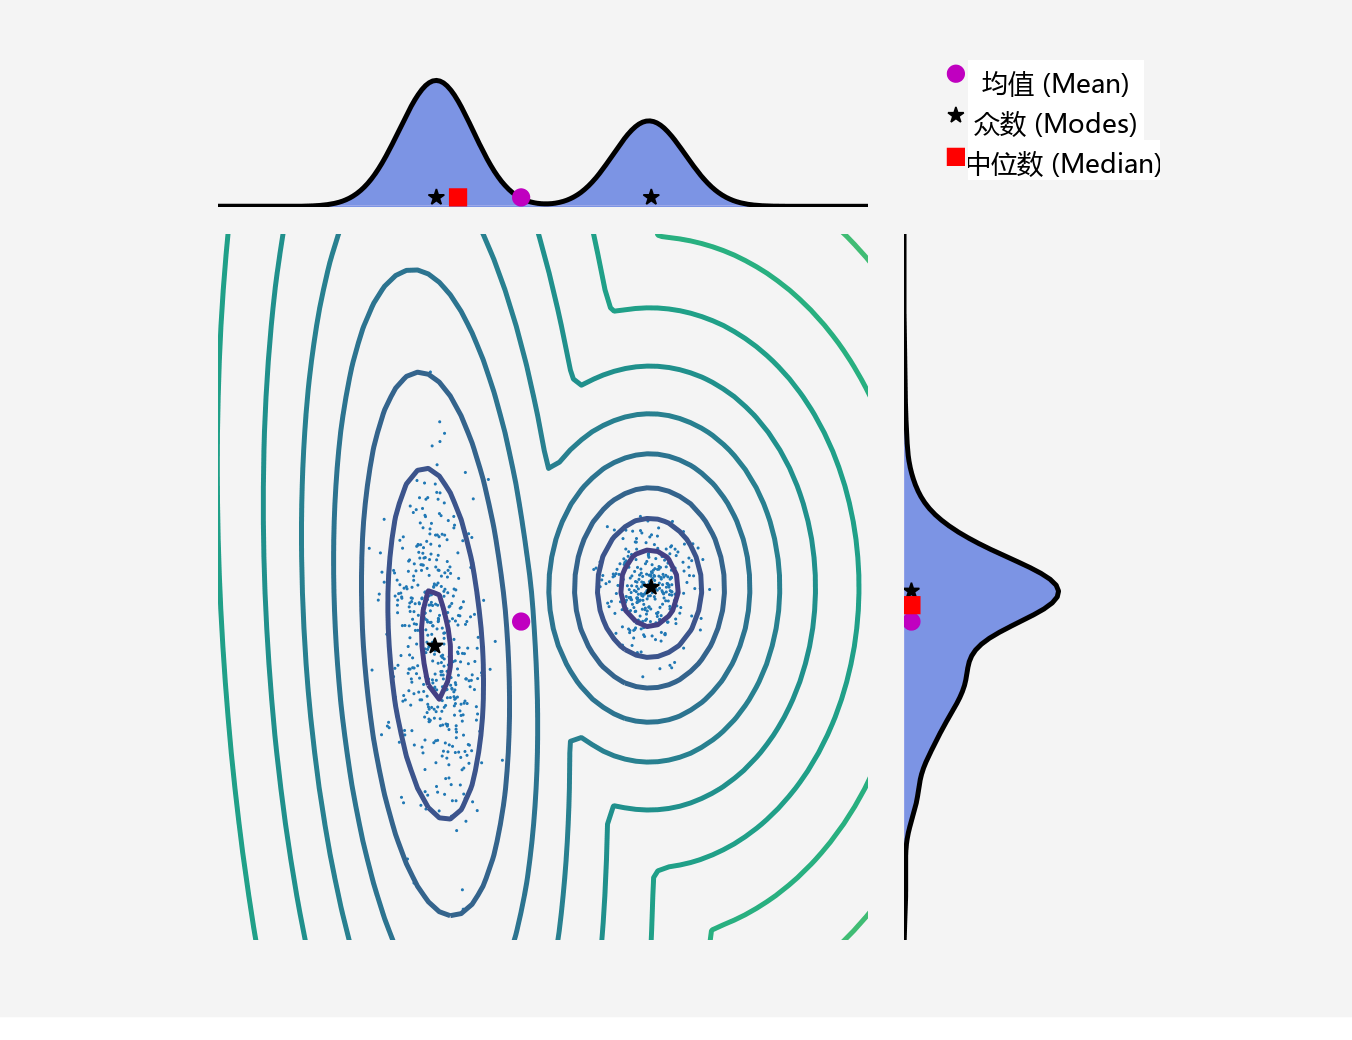
\includegraphics[width=0.92\textwidth,keepaspectratio]{docs/images/Figure6.4.png}
\caption*{\refstepcounter{figcounter}\label{fig:6-4}图~\thefigcounter 二维数据集的均值、众数与中位数，以及其边缘密度的示意图。}
\end{figure}


\emph{备注} 。期望值（定义 6.3）是一个线性算子。例如，给定实值函数 $ f(\boldsymbol{x}) = a g(\boldsymbol{x}) + b h(\boldsymbol{x}) $，其中 $ a, b \in \mathbb{R} $ 且 $ \boldsymbol{x} \in \mathbb{R}^D $，我们得到：

\begin{equation}
\mathbb{E}_{\boldsymbol{X}}[f(\boldsymbol{x})] = \int f(\boldsymbol{x}) p(\boldsymbol{x})\,\mathrm{d}\boldsymbol{x}
\tag{6.34a}\label{eq:6-34a}
\end{equation}

\begin{equation}
= \int [a g(\boldsymbol{x}) + b h(\boldsymbol{x})] p(\boldsymbol{x})\,\mathrm{d}\boldsymbol{x}
\tag{6.34b}\label{eq:6-34b}
\end{equation}

\begin{equation}
= a \int g(\boldsymbol{x}) p(\boldsymbol{x})\,\mathrm{d}\boldsymbol{x} + b \int h(\boldsymbol{x}) p(\boldsymbol{x})\,\mathrm{d}\boldsymbol{x}
\tag{6.34c}\label{eq:6-34c}
\end{equation}

\begin{equation}
= a \mathbb{E}_{\boldsymbol{X}}[g(\boldsymbol{x})] + b \mathbb{E}_{\boldsymbol{X}}[h(\boldsymbol{x})]
\tag{6.34d}\label{eq:6-34d}
\end{equation}

♦

对于两个随机变量，我们可能希望刻画它们之间的对应关联。协方差直观地表示了随机变量之间相互依赖程度的概念。

\textbf{定义 6.5}（单变量协方差）。两个单变量随机变量 $ X, Y \in \mathbb{R} $ 之间的 \emph{协方差（covariance）} 给出为它们各自偏离其均值的偏差乘积的期望值，即：

\begin{equation}
\mathrm{Cov}_{X,Y}[x, y] := \mathbb{E}_{X,Y}\big[(x - \mathbb{E}_X[x])(y - \mathbb{E}_Y[y])\big]
\tag{6.35}\label{eq:6-35}
\end{equation}

术语说明：多元随机变量的协方差 $ \mathrm{Cov}[\boldsymbol{x}, \boldsymbol{y}] $ 有时被称为互协方差（cross-covariance），而协方差特指 $ \mathrm{Cov}[\boldsymbol{x}, \boldsymbol{x}] $。

\emph{备注} 。当与期望或协方差相关联的随机变量通过其自变量可以明确分辨时，通常省略下标（例如 $ \mathbb{E}_X[x] $ 常简记为 $ \mathbb{E}[x] $）。♦

利用期望的线性性质，定义 6.5 中的表达式可以重写为乘积的期望减去期望的乘积，即：

\begin{equation}
\mathrm{Cov}[x, y] = \mathbb{E}[xy] - \mathbb{E}[x]\mathbb{E}[y]
\tag{6.36}\label{eq:6-36}
\end{equation}

变量与其自身的协方差 $ \mathrm{Cov}[x, x] $ 称为 \emph{方差（variance）} ，记为 $ \mathbb{V}_X[x] $。方差的平方根称为 \emph{标准差（standard deviation）} ，通常记为 $ \sigma(x) $。协方差的概念可以推广到多元随机变量。

\textbf{定义 6.6}（多元协方差）。如果我们考虑两个多元随机变量 $ \boldsymbol{X} $ 和 $ \boldsymbol{Y} $，其状态分别处于 $ \boldsymbol{x} \in \mathbb{R}^D $ 和 $ \boldsymbol{y} \in \mathbb{R}^E $，则 $ \boldsymbol{X} $ 与 $ \boldsymbol{Y} $ 之间的 \emph{协方差（covariance）} 定义为：

\begin{equation}
\begin{adjustbox}{max width=\linewidth}
\mathrm{Cov}[\boldsymbol{x}, \boldsymbol{y}] = \mathbb{E}[\boldsymbol{x} \boldsymbol{y}^\top] - \mathbb{E}[\boldsymbol{x}]\mathbb{E}[\boldsymbol{y}]^\top = \mathrm{Cov}[\boldsymbol{y}, \boldsymbol{x}]^\top \in \mathbb{R}^{D \times E}
\end{adjustbox}
\tag{6.37}\label{eq:6-37}
\end{equation}

定义 6.6 可以将相同的多元随机变量同时作为两个自变量输入，由此产生了一个直观捕获随机变量“分散程度（spread）”的有用概念。对于多元随机变量，方差描述了随机变量各维度之间的关系。

\textbf{定义 6.7}（方差）。状态为 $ \boldsymbol{x} \in \mathbb{R}^D $ 且均值向量为 $ \boldsymbol{\mu} \in \mathbb{R}^D $ 的随机变量 $ \boldsymbol{X} $ 的 \emph{方差（variance）} 定义为：

\begin{equation}
\mathbb{V}_{\boldsymbol{X}}[\boldsymbol{x}] = \mathrm{Cov}_{\boldsymbol{X}}[\boldsymbol{x}, \boldsymbol{x}]
\tag{6.38a}\label{eq:6-38a}
\end{equation}

\begin{equation}
\begin{adjustbox}{max width=\linewidth}
= \mathbb{E}_{\boldsymbol{X}}\big[(\boldsymbol{x} - \boldsymbol{\mu})(\boldsymbol{x} - \boldsymbol{\mu})^\top\big] = \mathbb{E}_{\boldsymbol{X}}[\boldsymbol{x} \boldsymbol{x}^\top] - \mathbb{E}_{\boldsymbol{X}}[\boldsymbol{x}]\mathbb{E}_{\boldsymbol{X}}[\boldsymbol{x}]^\top
\end{adjustbox}
\tag{6.38b}\label{eq:6-38b}
\end{equation}

\begin{equation}
\begin{adjustbox}{max width=\linewidth}
= \begin{bmatrix} \mathrm{Cov}[x_1, x_1] & \mathrm{Cov}[x_1, x_2] & \cdots & \mathrm{Cov}[x_1, x_D] \\ \mathrm{Cov}[x_2, x_1] & \mathrm{Cov}[x_2, x_2] & \cdots & \mathrm{Cov}[x_2, x_D] \\ \vdots & \vdots & \ddots & \vdots \\ \mathrm{Cov}[x_D, x_1] & \cdots & \cdots & \mathrm{Cov}[x_D, x_D] \end{bmatrix}
\end{adjustbox}
\tag{6.38c}\label{eq:6-38c}
\end{equation}

式~\eqref{eq:6-38c} 中的 $ D \times D $ 矩阵称为多元随机变量 $ \boldsymbol{X} $ 的 \emph{协方差矩阵（covariance matrix）} 。协方差矩阵是对称且半正定的，它反映了数据的分散特征。在其对角线上，协方差矩阵包含边缘分布的方差：

\begin{equation}
p(x_i) = \int p(x_1, \ldots, x_D)\,\mathrm{d}\boldsymbol{x}_{\backslash i}
\tag{6.39}\label{eq:6-39}
\end{equation}

其中“$ \backslash i $”表示“除 $ i $ 以外的所有变量”。非对角线元素则是 \emph{互协方差（cross-covariance）} 项 $ \mathrm{Cov}[x_i, x_j] $（其中 $ i, j = 1, \ldots, D $ 且 $ i \ne j $）。


\begin{figure}[H]
\centering
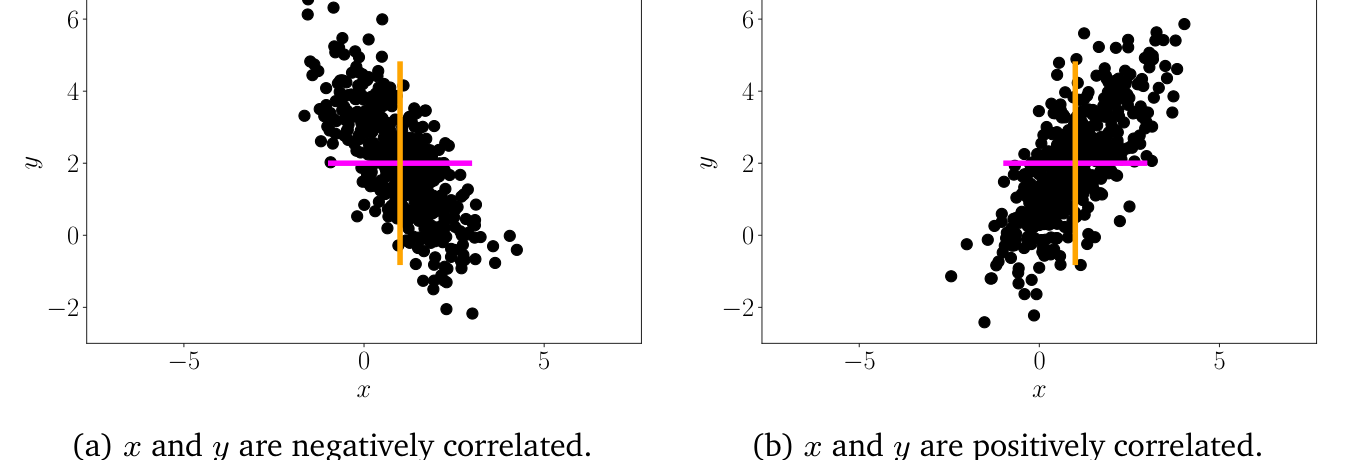
\includegraphics[width=0.92\textwidth,keepaspectratio]{docs/images/Figure6.5.png}
\caption*{\refstepcounter{figcounter}\label{fig:6-5}图~\thefigcounter 沿各轴具有相同均值和方差（彩色线所示）但具有不同协方差的二维数据集。(a) x 与 y 负相关；(b) x 与 y 正相关。}
\end{figure}


\emph{备注} 。在本书中，为了提供更好的几何直觉，我们通常假设协方差矩阵是正定的。因此我们不深入探讨导致半正定（低秩）协方差矩阵的极端边界情形。♦

当我们需要比较不同随机变量对之间的协方差时，每个随机变量自身的方差都会影响协方差的取值大小。协方差的归一化版本称为相关系数。

\textbf{定义 6.8}（相关系数）。两个随机变量 $ X, Y $ 之间的 \emph{相关系数（correlation）} 给出为：

\begin{equation}
\operatorname{corr}[x, y] = \frac{\mathrm{Cov}[x, y]}{\sqrt{\mathbb{V}[x]\mathbb{V}[y]}} \in [-1, 1]
\tag{6.40}\label{eq:6-40}
\end{equation}

相关矩阵是标准化随机变量 $ x / \sigma(x) $ 的协方差矩阵。换言之，在相关矩阵中，每个随机变量都被除以其自身的标准差（方差的平方根）。

协方差（与相关系数）表明了两个随机变量之间的关联方式；参见图~\ref{fig:6-5}。正相关 $ \operatorname{corr}[x, y] > 0 $ 意味着当 $ x $ 增长时，$ y $ 预计也会随之增长。负相关意味着随着 $ x $ 增加，$ y $ 会减少。

\medskip\hrule\medskip

\section*{6.4.2 经验均值与经验协方差}
\addcontentsline{toc}{subsection}{6.4.2 经验均值与经验协方差}

第 6.4.1 节中的定义通常也称为 \emph{总体均值（population mean）} 和 \emph{总体协方差（population covariance）} ，因为它们指代的是总体的真实统计量。在机器学习中，我们需要从经验数据观测中进行学习。考虑一个随机变量 $ X $。从总体统计量到经验统计量的实现存在两个概念步骤。首先，利用我们拥有有限数据集（大小为 $ N $）这一事实，构建一个作为有限个同分布独立随机变量 $ X_1, \ldots, X_N $ 之函数的经验统计量。其次，我们观测数据，即观察每个随机变量的具体实现值 $ x_1, \ldots, x_N $ 并应用该经验统计量。

具体而言，对于均值（定义 6.4），给定一个具体的数据集，我们可以获得均值的一个估计，称为 \emph{经验均值（empirical mean）} 或 \emph{样本均值（sample mean）} 。经验协方差也是同理。

\textbf{定义 6.9}（经验均值与经验协方差）。经验均值向量是每个变量观测值的算术平均值，定义为：

\begin{equation}
\bar{\boldsymbol{x}} := \frac{1}{N} \sum_{n=1}^N \boldsymbol{x}_n
\tag{6.41}\label{eq:6-41}
\end{equation}

其中 $ \boldsymbol{x}_n \in \mathbb{R}^D $。

与经验均值类似， \emph{经验协方差矩阵（empirical covariance matrix）} 是一个 $ D \times D $ 矩阵：

\begin{equation}
\boldsymbol{\Sigma} := \frac{1}{N} \sum_{n=1}^N (\boldsymbol{x}_n - \bar{\boldsymbol{x}})(\boldsymbol{x}_n - \bar{\boldsymbol{x}})^\top
\tag{6.42}\label{eq:6-42}
\end{equation}

在全书中，我们使用经验协方差，它是一个有偏估计。无偏（有时称为校正后的）协方差在分母中使用因子 $ N - 1 $ 而不是 $ N $。

为了计算具体数据集的统计量，我们将使用具体实现（观测值）$ \boldsymbol{x}_1, \ldots, \boldsymbol{x}_N $ 并应用式~\eqref{eq:6-41} 和式~\eqref{eq:6-42}。经验协方差矩阵是对称且半正定的（见第 3.2.3 节）。

\medskip\hrule\medskip

\section*{6.4.3 方差的三种表达式}
\addcontentsline{toc}{subsection}{6.4.3 方差的三种表达式}

我们现在聚焦于单个随机变量 $ X $，并利用前述经验公式推导出方差的三种可能表达式。以下推导同样适用于总体方差，只需注意将求和替换为积分。这些推导构成本章末尾的习题。

方差的标准定义对应于协方差的定义（定义 6.5），是随机变量 $ X $ 偏离其期望值 $ \mu $ 的偏差平方的期望，即：

\begin{equation}
\mathbb{V}_X[x] := \mathbb{E}_X\big[(x - \mu)^2\big]
\tag{6.43}\label{eq:6-43}
\end{equation}

式~\eqref{eq:6-43} 中的期望和均值 $ \mu = \mathbb{E}_X[x] $ 依据 $ X $ 是离散还是连续随机变量，分别使用式~\eqref{eq:6-32} 计算。式~\eqref{eq:6-43} 所表示的方差即为新随机变量 $ Z := (X - \mu)^2 $ 的均值。

当通过经验数据估计式~\eqref{eq:6-43} 中的方差时，我们需要采用双遍（two-pass）算法：第一遍遍历数据利用式~\eqref{eq:6-41} 计算均值 $ \mu $，然后利用此估计值 $ \hat{\mu} $ 进行第二遍遍历以计算方差。事实证明，我们可以通过重新整理各项来避免双遍扫描。式~\eqref{eq:6-43} 中的公式可以转换为所谓的 \emph{方差的原始得分公式（raw-score formula for variance）} ：

\begin{equation}
\mathbb{V}_X[x] = \mathbb{E}_X[x^2] - \big(\mathbb{E}_X[x]\big)^2
\tag{6.44}\label{eq:6-44}
\end{equation}

式~\eqref{eq:6-44} 中的表达式可以通俗地记为“平方的均值减去均值的平方”。由于我们可以同时累加 $ x_i $（用于计算均值）和 $ x_i^2 $（其中 $ x_i $ 是第 $ i $ 个观测值），因此它可以在单遍（one pass）数据扫描中以经验方式计算。然而，如果以这种方式实现，可能会在数值上不稳定。如果式~\eqref{eq:6-44} 中的两项数值巨大且近似相等，我们在浮点运算中可能会遭受不必要的数值精度损失（巨灾抵消）。方差的原始得分版本在机器学习中非常有用，例如在推导偏差-方差分解时（Bishop, 2006）。

理解方差的第三种方式是将其视为所有观测对之间成对差值的平方和。考虑随机变量 $ X $ 的一组观测样本 $ x_1, \ldots, x_N $，我们计算 $ x_i $ 与 $ x_j $ 对之间的差值平方。通过展开平方项，我们可以证明 $ N^2 $ 个成对差值之和即为观测值的经验方差：

\begin{equation}
\frac{1}{N^2} \sum_{i,j=1}^N (x_i - x_j)^2 = 2 \left[ \frac{1}{N} \sum_{i=1}^N x_i^2 - \left( \frac{1}{N} \sum_{i=1}^N x_i \right)^2 \right]
\tag{6.45}\label{eq:6-45}
\end{equation}

我们看到式~\eqref{eq:6-45} 是原始得分表达式~\eqref{eq:6-44} 的两倍。这意味着我们可以将成对距离之和（共有 $ N^2 $ 项）表示为偏离均值的偏差之和（共有 $ N $ 项）。从几何上看，这意味着点集内部的成对距离与各点到点集中心的距离之间存在等价性。从计算角度来看，这意味着通过先计算均值（求和包含 $ N $ 项），然后再计算方差（求和同样包含 $ N $ 项），我们可以计算出包含 $ N^2 $ 项的表达式（式~\eqref{eq:6-45} 的左侧）。

\medskip\hrule\medskip

\section*{6.4.4 随机变量的和与变换}
\addcontentsline{toc}{subsection}{6.4.4 随机变量的和与变换}

我们可能希望对教科书标准分布（我们在第 6.5 节和第 6.6 节中会介绍一些）无法良好解释的现象进行建模，因此可能对随机变量执行简单操作（例如将两个随机变量相加）。

考虑两个状态为 $ \boldsymbol{x}, \boldsymbol{y} \in \mathbb{R}^D $ 的随机变量 $ \boldsymbol{X}, \boldsymbol{Y} $，则有：

\begin{equation}
\mathbb{E}[\boldsymbol{x} + \boldsymbol{y}] = \mathbb{E}[\boldsymbol{x}] + \mathbb{E}[\boldsymbol{y}]
\tag{6.46}\label{eq:6-46}
\end{equation}

\begin{equation}
\mathbb{E}[\boldsymbol{x} - \boldsymbol{y}] = \mathbb{E}[\boldsymbol{x}] - \mathbb{E}[\boldsymbol{y}]
\tag{6.47}\label{eq:6-47}
\end{equation}

\begin{equation}
\mathbb{V}[\boldsymbol{x} + \boldsymbol{y}] = \mathbb{V}[\boldsymbol{x}] + \mathbb{V}[\boldsymbol{y}] + \mathrm{Cov}[\boldsymbol{x}, \boldsymbol{y}] + \mathrm{Cov}[\boldsymbol{y}, \boldsymbol{x}]
\tag{6.48}\label{eq:6-48}
\end{equation}

\begin{equation}
\mathbb{V}[\boldsymbol{x} - \boldsymbol{y}] = \mathbb{V}[\boldsymbol{x}] + \mathbb{V}[\boldsymbol{y}] - \mathrm{Cov}[\boldsymbol{x}, \boldsymbol{y}] - \mathrm{Cov}[\boldsymbol{y}, \boldsymbol{x}]
\tag{6.49}\label{eq:6-49}
\end{equation}

当涉及随机变量的仿射变换时，均值和（协）方差展现出一些有用的性质。考虑具有均值 $ \boldsymbol{\mu} $ 和协方差矩阵 $ \boldsymbol{\Sigma} $ 的随机变量 $ \boldsymbol{X} $，以及 $ \boldsymbol{x} $ 的（确定性）仿射变换 $ \boldsymbol{y} = \boldsymbol{A}\boldsymbol{x} + \boldsymbol{b} $。那么 $ \boldsymbol{y} $ 本身也是一个随机变量，其均值向量和协方差矩阵分别给出为：

\begin{equation}
\begin{adjustbox}{max width=\linewidth}
\mathbb{E}_{\boldsymbol{Y}}[\boldsymbol{y}] = \mathbb{E}_{\boldsymbol{X}}[\boldsymbol{A}\boldsymbol{x} + \boldsymbol{b}] = \boldsymbol{A}\mathbb{E}_{\boldsymbol{X}}[\boldsymbol{x}] + \boldsymbol{b} = \boldsymbol{A}\boldsymbol{\mu} + \boldsymbol{b}
\end{adjustbox}
\tag{6.50}\label{eq:6-50}
\end{equation}

\begin{equation}
\begin{adjustbox}{max width=\linewidth}
\mathbb{V}_{\boldsymbol{Y}}[\boldsymbol{y}] = \mathbb{V}_{\boldsymbol{X}}[\boldsymbol{A}\boldsymbol{x} + \boldsymbol{b}] = \mathbb{V}_{\boldsymbol{X}}[\boldsymbol{A}\boldsymbol{x}] = \boldsymbol{A}\mathbb{V}_{\boldsymbol{X}}[\boldsymbol{x}]\boldsymbol{A}^\top = \boldsymbol{A}\boldsymbol{\Sigma}\boldsymbol{A}^\top
\end{adjustbox}
\tag{6.51}\label{eq:6-51}
\end{equation}

此外，直接利用均值和协方差的定义可以证明：

\begin{equation}
\begin{adjustbox}{max width=\linewidth}
\mathrm{Cov}[\boldsymbol{x}, \boldsymbol{y}] = \mathbb{E}\big[\boldsymbol{x}(\boldsymbol{A}\boldsymbol{x} + \boldsymbol{b})^\top\big] - \mathbb{E}[\boldsymbol{x}]\mathbb{E}[\boldsymbol{A}\boldsymbol{x} + \boldsymbol{b}]^\top
\end{adjustbox}
\tag{6.52a}\label{eq:6-52a}
\end{equation}

\begin{equation}
= \mathbb{E}[\boldsymbol{x}]\boldsymbol{b}^\top + \mathbb{E}[\boldsymbol{x}\boldsymbol{x}^\top]\boldsymbol{A}^\top - \boldsymbol{\mu}\boldsymbol{b}^\top - \boldsymbol{\mu}\boldsymbol{\mu}^\top\boldsymbol{A}^\top
\tag{6.52b}\label{eq:6-52b}
\end{equation}

\begin{equation}
= \boldsymbol{\mu}\boldsymbol{b}^\top - \boldsymbol{\mu}\boldsymbol{b}^\top + \big(\mathbb{E}[\boldsymbol{x}\boldsymbol{x}^\top] - \boldsymbol{\mu}\boldsymbol{\mu}^\top\big)\boldsymbol{A}^\top
\tag{6.52c}\label{eq:6-52c}
\end{equation}

\begin{equation}
\stackrel{(6.38\mathrm{b})}{=} \boldsymbol{\Sigma}\boldsymbol{A}^\top
\tag{6.52d}\label{eq:6-52d}
\end{equation}

其中 $ \boldsymbol{\Sigma} = \mathbb{E}[\boldsymbol{x}\boldsymbol{x}^\top] - \boldsymbol{\mu}\boldsymbol{\mu}^\top $ 是 $ \boldsymbol{X} $ 的协方差。

\medskip\hrule\medskip

\section*{6.4.5 统计独立性}
\addcontentsline{toc}{subsection}{6.4.5 统计独立性}

\textbf{定义 6.10}（独立性）。两个随机变量 $ X, Y $ 是 \emph{统计独立（statistically independent）} 的，当且仅当：

\begin{equation}
p(x, y) = p(x)p(y)
\tag{6.53}\label{eq:6-53}
\end{equation}

直观上，如果知道 $ y $ 的值不会为我们提供关于 $ x $ 的任何额外信息（反之亦然），则两个随机变量 $ X $ 和 $ Y $ 是独立的。若 $ X, Y $（统计）独立，则满足：

\begin{itemize}
\item $ p(y \mid x) = p(y) $
\item $ p(x \mid y) = p(x) $
\item $ \mathbb{V}_{X,Y}[x + y] = \mathbb{V}_X[x] + \mathbb{V}_Y[y] $
\item $ \mathrm{Cov}_{X,Y}[x, y] = 0 $
\end{itemize}

后一点反过来并不一定成立，即两个随机变量的协方差可以为零，但它们并不是统计独立的。为了理解其中的原因，请回想协方差仅度量线性相关性。因此，存在非线性依赖关系的随机变量其协方差完全可能为零。

\begin{notebox}
\textbf{例 6.5}
\end{notebox}

\begin{notebox}
考虑一个零均值（$ \mathbb{E}_X[x] = 0 $）且满足 $ \mathbb{E}_X[x^3] = 0 $ 的随机变量 $ X $。令 $ y = x^2 $（因此 $ Y $ 依赖于 $ X $），并考虑 $ X $ 与 $ Y $ 之间的协方差 (6.36)。由此可得：

\begin{equation}
\mathrm{Cov}[x, y] = \mathbb{E}[xy] - \mathbb{E}[x]\mathbb{E}[y] = \mathbb{E}[x^3] = 0
\tag{6.54}\label{eq:6-54}
\end{equation}
\end{notebox}

在机器学习中，我们经常考虑可以建模为 \emph{独立同分布（independent and identically distributed, i.i.d.）} 随机变量 $ X_1, \ldots, X_N $ 的问题。对于多于两个随机变量的情况，“独立”（定义 6.10）通常指代 \emph{相互独立（mutually independent）} 的随机变量，即其所有子集都是相互独立的（参见 Pollard (2002, 第 4 章) 和 Jacod and Protter (2004, 第 3 章)）。短语“同分布”意味着所有随机变量都来自同一个分布。

机器学习中另一个重要的概念是条件独立性。

\textbf{定义 6.11}（条件独立性）。在给定 $ Z $ 的条件下，两个随机变量 $ X $ 和 $ Y $ 是 \emph{条件独立（conditionally independent）} 的，当且仅当：

\begin{equation}
p(x, y \mid z) = p(x \mid z)p(y \mid z) \quad \textcn{对所有 } z \in \mathcal{Z}
\tag{6.55}\label{eq:6-55}
\end{equation}

其中 $ \mathcal{Z} $ 是随机变量 $ Z $ 的状态集。我们记作 $ X \perp\!\!\!\perp Y \mid Z $ 表示在给定 $ Z $ 时 $ X $ 与 $ Y $ 条件独立。

定义 6.11 要求式~\eqref{eq:6-55} 中的关系必须对 $ z $ 的每一个取值都成立。式~\eqref{eq:6-55} 可以解释为：“在获知关于 $ z $ 的知识后，$ x $ 和 $ y $ 的联合分布发生因子分解”。若写作 $ X \perp\!\!\!\perp Y \mid \emptyset $，无条件独立性可以被视为条件独立性的特例。利用概率的乘法法则 (6.22)，我们可以展开式~\eqref{eq:6-55} 的左边得到：

\begin{equation}
p(x, y \mid z) = p(x \mid y, z)p(y \mid z)
\tag{6.56}\label{eq:6-56}
\end{equation}

比较式~\eqref{eq:6-55} 的右侧与式~\eqref{eq:6-56}，我们发现两式均出现 $ p(y \mid z) $，从而有：

\begin{equation}
p(x \mid y, z) = p(x \mid z)
\tag{6.57}\label{eq:6-57}
\end{equation}

式~\eqref{eq:6-57} 提供了条件独立性（即 $ X \perp\!\!\!\perp Y \mid Z $）的另一种等价定义。这种表述方式具有清晰的直观解释：“已知 $ z $ 时，关于 $ y $ 的新知识不会改变我们对 $ x $ 的认知”。

\medskip\hrule\medskip

\section*{6.4.6 随机变量的内积}
\addcontentsline{toc}{subsection}{6.4.6 随机变量的内积}

回顾第 3.2 节中关于内积的定义。我们可以在随机变量之间定义内积，本节将对此进行简要阐述。多元随机变量之间的内积也可以采用类似的方式处理。

如果我们有两个不相关的随机变量 $ X, Y $，则：

\begin{equation}
\mathbb{V}[x + y] = \mathbb{V}[x] + \mathbb{V}[y]
\tag{6.58}\label{eq:6-58}
\end{equation}

由于方差是以平方单位计量的，这看起来非常类似于直角三角形的勾股定理 $ c^2 = a^2 + b^2 $。

接下来，我们将探讨能否为式~\eqref{eq:6-58} 中不相关随机变量的方差关系找到几何解释。


\begin{figure}[H]
\centering
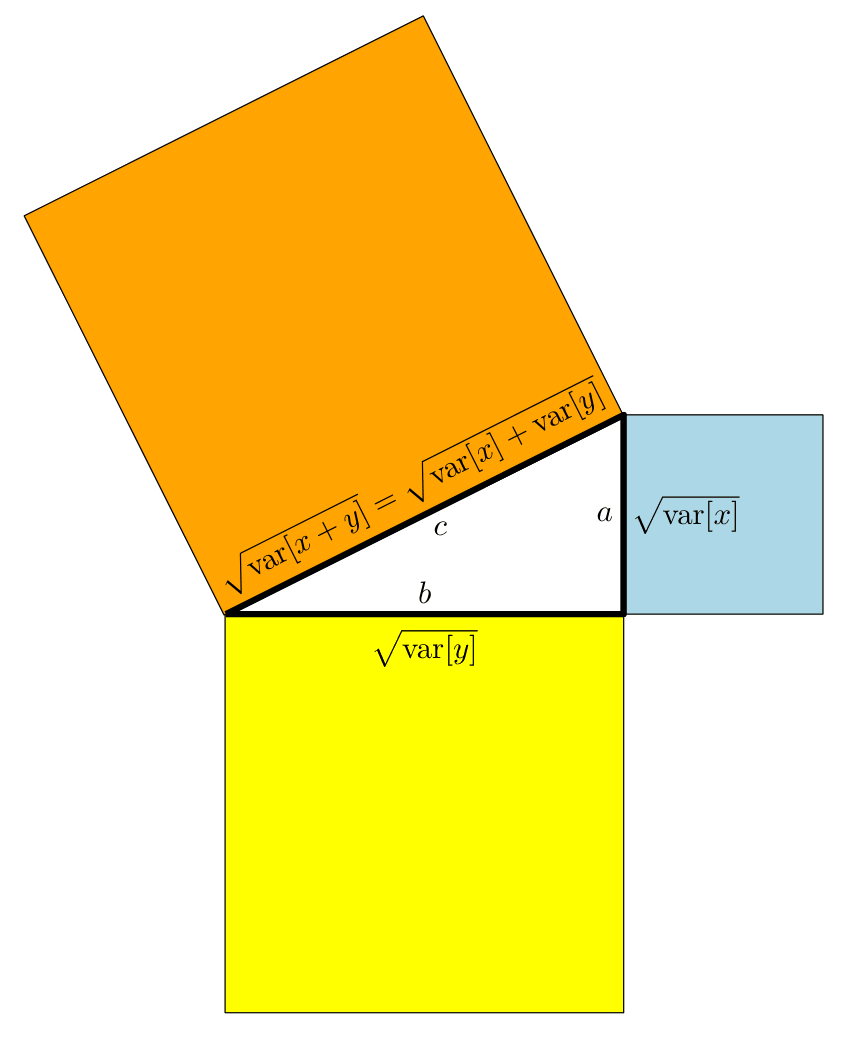
\includegraphics[width=320pt,keepaspectratio]{docs/images/Figure6.6.png}
\caption*{\refstepcounter{figcounter}\label{fig:6-6}图~\thefigcounter 随机变量的几何意义。若随机变量 X 和 Y 不相关，则它们在相应向量空间中是正交向量，且勾股定理成立。}
\end{figure}


随机变量可以被视为向量空间中的向量，我们可以定义内积以获取随机变量的几何性质（Eaton, 2007）。对于零均值随机变量 $ X $ 和 $ Y $，如果我们定义：

\begin{equation}
\langle X, Y \rangle := \mathrm{Cov}[x, y]
\tag{6.59}\label{eq:6-59}
\end{equation}

即可获得一个内积。我们看到协方差是对称的、正定的（$ \mathrm{Cov}[x, x] = 0 \iff x = 0 $），并且对任一自变量均满足线性（对任意 $ \alpha \in \mathbb{R} $，有 $ \mathrm{Cov}[\alpha x + z, y] = \alpha \mathrm{Cov}[x, y] + \mathrm{Cov}[z, y] $）。随机变量的“长度”为：

\begin{equation}
\|X\| = \sqrt{\mathrm{Cov}[x, x]} = \sqrt{\mathbb{V}[x]} = \sigma[x]
\tag{6.60}\label{eq:6-60}
\end{equation}

即为其标准差。随机变量越“长”，其不确定性就越大；而长度为 0 的随机变量则是确定性的。

如果我们观察两个随机变量 $ X, Y $ 之间的夹角 $ \theta $，可得：

\begin{equation}
\cos \theta = \frac{\langle X, Y \rangle}{\|X\|\,\|Y\|} = \frac{\mathrm{Cov}[x, y]}{\sqrt{\mathbb{V}[x]\mathbb{V}[y]}}
\tag{6.61}\label{eq:6-61}
\end{equation}

这正是两个随机变量之间的相关系数（定义 6.8）。这意味着，从几何角度来看，我们可以将相关系数视为两个随机变量之间夹角的余弦值。由定义 3.7 可知，$ X \perp Y \iff \langle X, Y \rangle = 0 $。在我们的情形中，这意味着 $ X $ 与 $ Y $ 正交当且仅当 $ \mathrm{Cov}[x, y] = 0 $，即它们是不相关的。图~\ref{fig:6-6} 说明了这种对应关系。

\emph{备注} 。尽管人们很容易尝试利用欧氏距离（基于前述内积定义构建）来比较概率分布，但遗憾的是，这并不是获取分布之间距离的最佳方式。回想一下，概率质量（或密度）是非负的，且总和必须为 1。这些约束意味着概率分布存在于所谓的 \emph{统计流形（statistical manifold）} 上。研究这种概率分布空间的学科称为 \emph{信息几何（information geometry）} 。计算分布之间的距离通常使用 \emph{Kullback-Leibler 散度（Kullback-Leibler divergence, KL 散度）} ，它是考虑了统计流形性质的距离推广。正如欧氏距离是度量的一个特例（第 3.3 节），Kullback-Leibler 散度也是两个更广泛散度族（称为 \emph{Bregman 散度（Bregman divergences）} 和 \emph{f-散度（f-divergences）} ）的特例。关于散度的深入研究超出了本书的范围，更多细节请参阅信息几何领域的先驱之一 Amari (2016) 的最新专著。♦

\section*{6.5 高斯分布}
\addcontentsline{toc}{section}{6.5 高斯分布}
\label{sec:6.5}

\emph{高斯分布（Gaussian distribution）} 是连续型随机变量中研究得最为透彻的概率分布。它也被称为 \emph{正态分布（normal distribution）} 。（ \emph{边注} ：当我们考虑独立同分布随机变量的和时，高斯分布会自然出现。这被称为 \emph{中心极限定理（central limit theorem）} (Grinstead and Snell, 1997)。）高斯分布的重要性源于它具有许多计算上极为便利的性质，我们将在下文中对此进行讨论。具体而言，我们将利用它来定义线性回归的似然函数与先验分布（第 9 章），并考虑使用高斯混合模型来进行密度估计（第 11 章）。

机器学习中的许多其他领域也受益于使用高斯分布，例如高斯过程（Gaussian processes）、变分推断（variational inference）和强化学习（reinforcement learning）。它还在其他应用领域中得到广泛使用，例如信号处理（如卡尔曼滤波，Kalman filter）、控制理论（如线性二次调节器，linear quadratic regulator）以及统计学（如假设检验，hypothesis testing）。

对于单变量随机变量，高斯分布的概率密度由下式给出：

\begin{equation}
p(x \mid \mu, \sigma^2) = \frac{1}{\sqrt{2\pi\sigma^2}} \exp\left( -\frac{(x - \mu)^2}{2\sigma^2} \right) .
\tag{6.62}\label{eq:6-62}
\end{equation}

\emph{多元高斯分布（multivariate Gaussian distribution）} （亦称 \emph{多元正态分布（multivariate normal distribution）} ）完全由 \emph{均值向量（mean vector）} $ \boldsymbol{\mu} $ 和 \emph{协方差矩阵（covariance matrix）} $ \boldsymbol{\Sigma} $ 表征，其定义为：

\begin{equation}
\begin{adjustbox}{max width=\linewidth}
p(\boldsymbol{x} \mid \boldsymbol{\mu}, \boldsymbol{\Sigma}) = (2\pi)^{-\frac{D}{2}} |\boldsymbol{\Sigma}|^{-\frac{1}{2}} \exp\left( -\frac{1}{2}(\boldsymbol{x} - \boldsymbol{\mu})^\top \boldsymbol{\Sigma}^{-1} (\boldsymbol{x} - \boldsymbol{\mu}) \right)
\end{adjustbox}
\tag{6.63}\label{eq:6-63}
\end{equation}

其中 $ \boldsymbol{x} \in \mathbb{R}^D $。我们记作 $ p(\boldsymbol{x}) = \mathcal{N}(\boldsymbol{x} \mid \boldsymbol{\mu}, \boldsymbol{\Sigma}) $ 或 $ \boldsymbol{X} \sim \mathcal{N}(\boldsymbol{\mu}, \boldsymbol{\Sigma}) $。图~\ref{fig:6-7} 展示了一个二元高斯分布（网格曲面）及其对应的等高线图。图~\ref{fig:6-8} 展示了一个单变量高斯分布和一个二元高斯分布以及相应的样本点。均值为零且协方差为单位矩阵的特殊高斯分布情形，即 $ \boldsymbol{\mu} = \boldsymbol{0} $ 且 $ \boldsymbol{\Sigma} = \boldsymbol{I} $，被称为 \emph{标准正态分布（standard normal distribution）} 。


\begin{figure}[H]
\centering
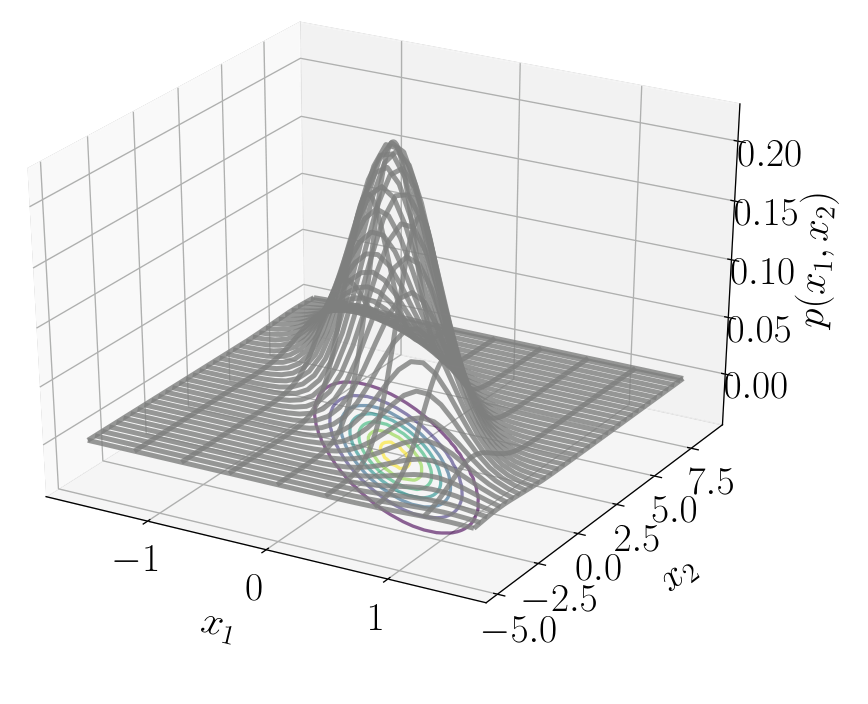
\includegraphics[width=0.92\textwidth,keepaspectratio]{docs/images/Figure6.7.png}
\caption*{\refstepcounter{figcounter}\label{fig:6-7}图~\thefigcounter 两个随机变量 x₁ 和 x₂ 的高斯分布。}
\end{figure}



\begin{figure}[H]
\centering
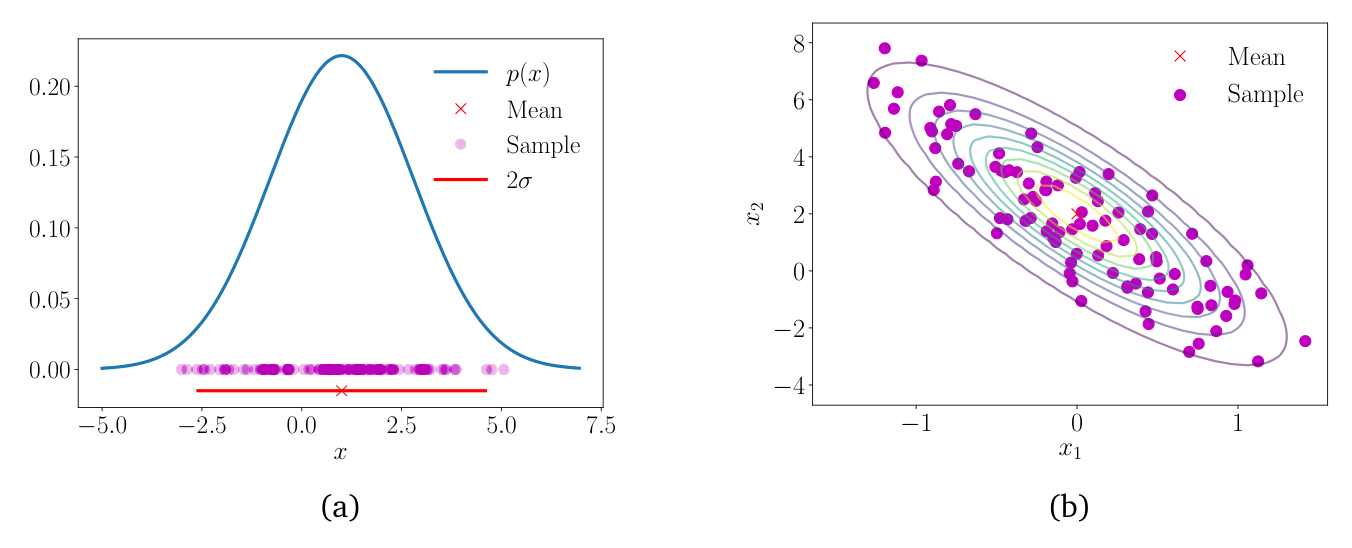
\includegraphics[width=0.92\textwidth,keepaspectratio]{docs/images/Figure6.8.png}
\caption*{\refstepcounter{figcounter}\label{fig:6-8}图~\thefigcounter 叠加了 100 个样本的高斯分布。(a) 一维（单变量）高斯分布，红十字表示均值，红线表示方差的范围；(b) 二维（多元）高斯分布的俯视图，红十字表示均值，彩色线条表示密度的等高线。}
\end{figure}


高斯分布在统计估计和机器学习中得到了极其广泛的应用，因为它们的边缘分布和条件分布都具有解析闭式表达式。在第 9 章中，我们将在线性回归中广泛使用这些闭式表达式。使用高斯随机变量进行建模的一个主要优势在于，通常不需要进行变量变换（第 6.7 节）。由于高斯分布完全由其均值和协方差决定，我们通常只需将变换直接应用于随机变量的均值和协方差，即可获得变换后的分布。

\medskip\hrule\medskip

\section*{6.5.1 高斯分布的边缘分布与条件分布仍为高斯分布}
\addcontentsline{toc}{subsection}{6.5.1 高斯分布的边缘分布与条件分布仍为高斯分布}

下面，我们介绍多元随机变量在一般情形下的边缘化和条件化。如果在初次阅读时感到困惑，建议读者先考虑两个单变量随机变量的情形。设 $ \boldsymbol{X} $ 和 $ \boldsymbol{Y} $ 为两个多元随机变量，它们可能具有不同的维度。为了考虑应用概率加法法则的效果以及条件化的效果，我们将高斯分布显式地写为拼接状态 $ [\boldsymbol{x}, \boldsymbol{y}]^\top $ 的形式：

\begin{equation}
\begin{adjustbox}{max width=\linewidth}
p(\boldsymbol{x}, \boldsymbol{y}) = \mathcal{N}\left( \begin{bmatrix} \boldsymbol{\mu}_x \\ \boldsymbol{\mu}_y \end{bmatrix}, \begin{bmatrix} \boldsymbol{\Sigma}_{xx} & \boldsymbol{\Sigma}_{xy} \\ \boldsymbol{\Sigma}_{yx} & \boldsymbol{\Sigma}_{yy} \end{bmatrix} \right)
\end{adjustbox}
\tag{6.64}\label{eq:6-64}
\end{equation}

其中 $ \boldsymbol{\Sigma}_{xx} = \mathrm{Cov}[\boldsymbol{x}, \boldsymbol{x}] $ 和 $ \boldsymbol{\Sigma}_{yy} = \mathrm{Cov}[\boldsymbol{y}, \boldsymbol{y}] $ 分别是 $ \boldsymbol{x} $ 和 $ \boldsymbol{y} $ 的边缘协方差矩阵，而 $ \boldsymbol{\Sigma}_{xy} = \mathrm{Cov}[\boldsymbol{x}, \boldsymbol{y}] $ 是 $ \boldsymbol{x} $ 与 $ \boldsymbol{y} $ 之间的 \emph{互协方差矩阵（cross-covariance matrix）} （且 $ \boldsymbol{\Sigma}_{yx} = \boldsymbol{\Sigma}_{xy}^\top $）。

条件分布 $ p(\boldsymbol{x} \mid \boldsymbol{y}) $ 也是高斯分布（如图~\ref{fig:6-9}(c) 所示），由下式给出（推导参见 Bishop (2006) 第 2.3 节）：

\begin{equation}
p(\boldsymbol{x} \mid \boldsymbol{y}) = \mathcal{N}(\boldsymbol{\mu}_{x \mid y}, \boldsymbol{\Sigma}_{x \mid y})
\tag{6.65}\label{eq:6-65}
\end{equation}

\begin{equation}
\boldsymbol{\mu}_{x \mid y} = \boldsymbol{\mu}_x + \boldsymbol{\Sigma}_{xy}\boldsymbol{\Sigma}_{yy}^{-1}(\boldsymbol{y} - \boldsymbol{\mu}_y)
\tag{6.66}\label{eq:6-66}
\end{equation}

\begin{equation}
\boldsymbol{\Sigma}_{x \mid y} = \boldsymbol{\Sigma}_{xx} - \boldsymbol{\Sigma}_{xy}\boldsymbol{\Sigma}_{yy}^{-1}\boldsymbol{\Sigma}_{yx} .
\tag{6.67}\label{eq:6-67}
\end{equation}

注意，在式~\eqref{eq:6-66} 的均值计算中，$ \boldsymbol{y} $ 的值是一个观测值，不再是随机的。

\emph{备注} 。条件高斯分布在我们需要求后验分布的许多场景中都会出现：

\begin{itemize}
\item 卡尔曼滤波（Kalman filter, Kalman, 1960）：信号处理中状态估计最核心的算法之一，其本质就是在计算联合分布的高斯条件分布（Deisenroth and Ohlsson, 2011; Särkkä, 2013）。
\item 高斯过程（Gaussian processes, Rasmussen and Williams, 2006）：函数空间分布的一种实际实现。在高斯过程中，我们假设随机变量服从联合高斯分布。通过对观测数据进行（高斯）条件化，我们可以确定函数空间上的后验分布。
\item 隐线性高斯模型（latent linear Gaussian models, Roweis and Ghahramani, 1999; Murphy, 2012）：包括概率主成分分析（probabilistic principal component analysis, PPCA, Tipping and Bishop, 1999）。我们将在第 10.7 节更详细地探讨 PPCA。♦
\end{itemize}

联合高斯分布 $ p(\boldsymbol{x}, \boldsymbol{y}) $（参见式~\eqref{eq:6-64}）的边缘分布 $ p(\boldsymbol{x}) $ 本身也是高斯分布，可以通过应用加法法则（式~\eqref{eq:6-20}）计算得到：

\begin{equation}
p(\boldsymbol{x}) = \int p(\boldsymbol{x}, \boldsymbol{y}) \mathrm{d}\boldsymbol{y} = \mathcal{N}(\boldsymbol{x} \mid \boldsymbol{\mu}_x, \boldsymbol{\Sigma}_{xx}) .
\tag{6.68}\label{eq:6-68}
\end{equation}

对 $ \boldsymbol{x} $ 进行边缘化可得到关于 $ p(\boldsymbol{y}) $ 的相应结论。直观地说，审视式~\eqref{eq:6-64} 中的联合分布，我们忽略了（即积分积掉）我们不感兴趣的所有内容。这在图~\ref{fig:6-9}(b) 中进行了说明。


\begin{figure}[H]
\centering
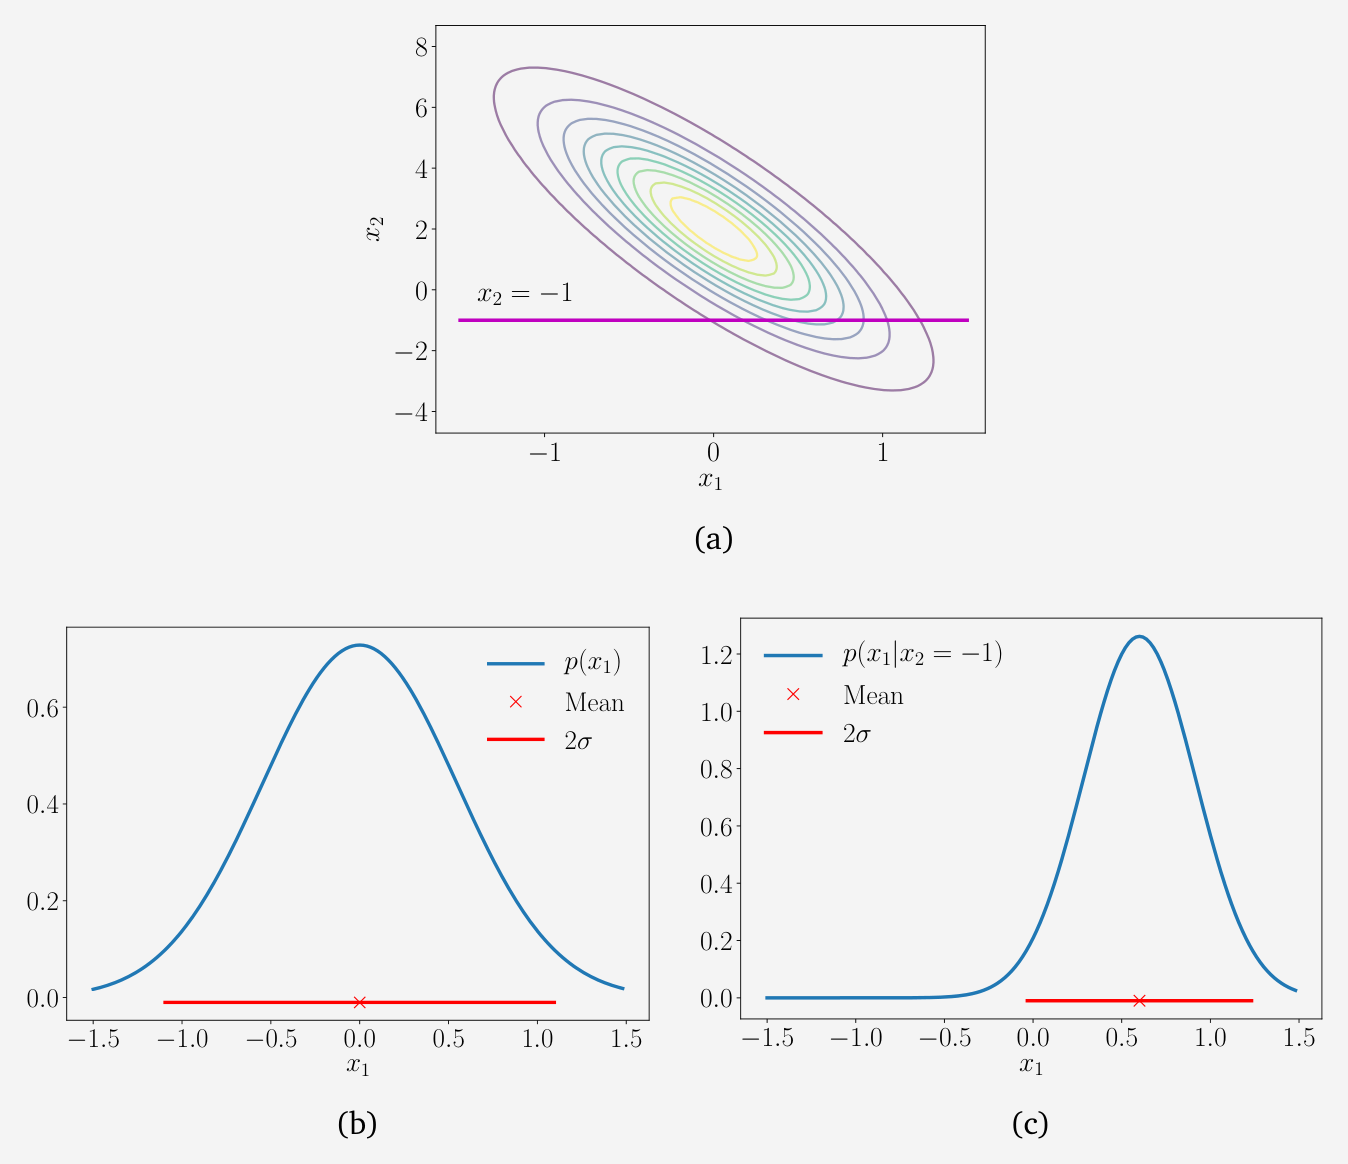
\includegraphics[width=0.92\textwidth,keepaspectratio]{docs/images/Figure6.9.png}
\caption*{\refstepcounter{figcounter}\label{fig:6-9}图~\thefigcounter (a) 二元高斯分布；(b) 联合高斯分布的边缘分布是高斯分布；(c) 高斯分布的条件分布也是高斯分布。}
\end{figure}


\begin{notebox}
\textbf{例 6.6}
\end{notebox}

\begin{notebox}
考虑二元高斯分布（如图~\ref{fig:6-9} 所示）：

\begin{equation}
p(x_1, x_2) = \mathcal{N}\left( \begin{bmatrix} 0 \\ 2 \end{bmatrix}, \begin{bmatrix} 0.3 & -1 \\ -1 & 5 \end{bmatrix} \right) .
\tag{6.69}\label{eq:6-69}
\end{equation}

我们可以通过应用式~\eqref{eq:6-66} 和式~\eqref{eq:6-67} 分别计算以 $ x_2 = -1 $ 为条件时的单变量高斯分布的均值和方差。数值计算如下：

\begin{equation}
\mu_{x_1 \mid x_2 = -1} = 0 + (-1) \cdot 0.2 \cdot (-1 - 2) = 0.6
\tag{6.70}\label{eq:6-70}
\end{equation}

以及

\begin{equation}
\sigma_{x_1 \mid x_2 = -1}^2 = 0.3 - (-1) \cdot 0.2 \cdot (-1) = 0.1 .
\tag{6.71}\label{eq:6-71}
\end{equation}

因此，条件高斯分布由下式给出：

\begin{equation}
p(x_1 \mid x_2 = -1) = \mathcal{N}(0.6, 0.1) .
\tag{6.72}\label{eq:6-72}
\end{equation}

相比之下，边缘分布 $ p(x_1) $ 可以通过应用式~\eqref{eq:6-68} 获得，这本质上是直接使用随机变量 $ x_1 $ 的均值和方差，得到：

\begin{equation}
p(x_1) = \mathcal{N}(0, 0.3) .
\tag{6.73}\label{eq:6-73}
\end{equation}
\end{notebox}

\medskip\hrule\medskip

\section*{6.5.2 高斯密度的乘积}
\addcontentsline{toc}{subsection}{6.5.2 高斯密度的乘积}

在进行线性回归时（第 9 章），我们需要计算高斯似然。此外，我们可能还希望设定高斯先验（第 9.3 节）。我们应用贝叶斯定理来计算后验分布，这将导致似然与先验相乘，即两个高斯密度的乘积。两个高斯分布 $ \mathcal{N}(\boldsymbol{x} \mid \boldsymbol{a}, \boldsymbol{A})\mathcal{N}(\boldsymbol{x} \mid \boldsymbol{b}, \boldsymbol{B}) $ 的乘积是一个乘以尺度因子 $ c \in \mathbb{R} $ 的高斯分布（ \emph{边注} ：该公式的推导见本章末尾的习题。），给出为 $ c \mathcal{N}(\boldsymbol{x} \mid \boldsymbol{c}, \boldsymbol{C}) $，其中：

\begin{equation}
\boldsymbol{C} = (\boldsymbol{A}^{-1} + \boldsymbol{B}^{-1})^{-1}
\tag{6.74}\label{eq:6-74}
\end{equation}

\begin{equation}
\boldsymbol{c} = \boldsymbol{C}(\boldsymbol{A}^{-1}\boldsymbol{a} + \boldsymbol{B}^{-1}\boldsymbol{b})
\tag{6.75}\label{eq:6-75}
\end{equation}

\begin{equation}
c = (2\pi)^{-\frac{D}{2}} |\boldsymbol{A} + \boldsymbol{B}|^{-\frac{1}{2}} \exp\left( -\frac{1}{2}(\boldsymbol{a} - \boldsymbol{b})^\top(\boldsymbol{A} + \boldsymbol{B})^{-1}(\boldsymbol{a} - \boldsymbol{b}) \right) .
\tag{6.76}\label{eq:6-76}
\end{equation}

尺度常数 $ c $ 本身也可以写成以 $ \boldsymbol{a} $ 或 $ \boldsymbol{b} $ 为自变量、协方差矩阵“膨胀”为 $ \boldsymbol{A} + \boldsymbol{B} $ 的高斯密度的形式，即

\begin{equation*}
c = \mathcal{N}(\boldsymbol{a} \mid \boldsymbol{b}, \boldsymbol{A} + \boldsymbol{B}) = \mathcal{N}(\boldsymbol{b} \mid \boldsymbol{a}, \boldsymbol{A} + \boldsymbol{B})
\end{equation*}

。

\emph{备注} 。为了符号上的便利，我们有时会使用 $ \mathcal{N}(\boldsymbol{x} \mid \boldsymbol{m}, \boldsymbol{S}) $ 来描述高斯密度的函数形式，即使 $ \boldsymbol{x} $ 并不是随机变量。我们在前面的展示中正是这样做的，当时我们写道：

\begin{equation}
c = \mathcal{N}(\boldsymbol{a} \mid \boldsymbol{b}, \boldsymbol{A} + \boldsymbol{B}) = \mathcal{N}(\boldsymbol{b} \mid \boldsymbol{a}, \boldsymbol{A} + \boldsymbol{B}) .
\tag{6.77}\label{eq:6-77}
\end{equation}

在这里，$ \boldsymbol{a} $ 和 $ \boldsymbol{b} $ 都不是随机变量。然而，以这种方式书写 $ c $ 比式~\eqref{eq:6-76} 更紧凑。♦

\medskip\hrule\medskip

\section*{6.5.3 和与线性变换}
\addcontentsline{toc}{subsection}{6.5.3 和与线性变换}

如果 $ \boldsymbol{X}, \boldsymbol{Y} $ 是相互独立的高斯随机变量（即联合分布给出为 $ p(\boldsymbol{x}, \boldsymbol{y}) = p(\boldsymbol{x})p(\boldsymbol{y}) $），且 $ p(\boldsymbol{x}) = \mathcal{N}(\boldsymbol{x} \mid \boldsymbol{\mu}_x, \boldsymbol{\Sigma}_x) $，$ p(\boldsymbol{y}) = \mathcal{N}(\boldsymbol{y} \mid \boldsymbol{\mu}_y, \boldsymbol{\Sigma}_y) $，那么 $ \boldsymbol{x} + \boldsymbol{y} $ 也服从高斯分布，并由下式给出：

\begin{equation}
p(\boldsymbol{x} + \boldsymbol{y}) = \mathcal{N}(\boldsymbol{\mu}_x + \boldsymbol{\mu}_y, \boldsymbol{\Sigma}_x + \boldsymbol{\Sigma}_y) .
\tag{6.78}\label{eq:6-78}
\end{equation}

已知 $ p(\boldsymbol{x} + \boldsymbol{y}) $ 是高斯分布后，可以直接利用式~\eqref{eq:6-46} 至式~\eqref{eq:6-49} 的结果确定其均值和协方差矩阵。当我们考虑作用在随机变量上的独立同分布（i.i.d.）高斯噪声时，这一性质将非常重要，例如线性回归中的情形（第 9 章）。

\begin{notebox}
\textbf{例 6.7}
\end{notebox}

\begin{notebox}
由于期望是线性算子，我们可以得到独立高斯随机变量的加权和：

\begin{equation}
p(a\boldsymbol{x} + b\boldsymbol{y}) = \mathcal{N}(a\boldsymbol{\mu}_x + b\boldsymbol{\mu}_y, a^2\boldsymbol{\Sigma}_x + b^2\boldsymbol{\Sigma}_y) .
\tag{6.79}\label{eq:6-79}
\end{equation}
\end{notebox}

\emph{备注} 。在第 11 章中非常有用的一个情形是高斯密度的加权和。这与高斯随机变量的加权和是截然不同的。♦

在定理 6.12 中，随机变量 $ x $ 来自由两个概率密度 $ p_1(x) $ 和 $ p_2(x) $ 以 $ \alpha $ 为权重混合而成的密度。由于期望的线性性质对多元随机变量同样成立，因此该定理可以推广到多元随机变量的情形。然而，随机变量平方的概念需要替换为 $ \boldsymbol{x} \boldsymbol{x}^\top $。

\textbf{定理 6.12}。考虑两个单变量高斯密度的混合：

\begin{equation}
p(x) = \alpha p_1(x) + (1 - \alpha)p_2(x)
\tag{6.80}\label{eq:6-80}
\end{equation}

其中标量 $ 0 < \alpha < 1 $ 为混合权重，$ p_1(x) $ 和 $ p_2(x) $ 是具有不同参数的单变量高斯密度（式~\eqref{eq:6-62}），即 $ (\mu_1, \sigma_1^2) \neq (\mu_2, \sigma_2^2) $。 则混合密度 $ p(x) $ 的均值由各个随机变量均值的加权和给出：

\begin{equation}
\mathbb{E}[x] = \alpha \mu_1 + (1 - \alpha)\mu_2 .
\tag{6.81}\label{eq:6-81}
\end{equation}

混合密度 $ p(x) $ 的方差由下式给出：

\begin{equation}
\mathbb{V}[x] = [\alpha\sigma_1^2 + (1 - \alpha)\sigma_2^2] + [\alpha\mu_1^2 + (1 - \alpha)\mu_2^2] - [\alpha\mu_1 + (1 - \alpha)\mu_2]^2 .
\tag{6.82}\label{eq:6-82}
\end{equation}

\textbf{证明}： 混合密度 $ p(x) $ 的均值由各个随机变量均值的加权和给出。我们应用均值的定义（定义 6.4），代入混合分布 (6.80)，得到：

\begin{equation}
\mathbb{E}[x] = \int_{-\infty}^\infty x p(x) \mathrm{d}x
\tag{6.83a}\label{eq:6-83a}
\end{equation}

\begin{equation}
= \int_{-\infty}^\infty \left[\alpha x p_1(x) + (1 - \alpha) x p_2(x)\right] \mathrm{d}x
\tag{6.83b}\label{eq:6-83b}
\end{equation}

\begin{equation}
= \alpha \int_{-\infty}^\infty x p_1(x) \mathrm{d}x + (1 - \alpha) \int_{-\infty}^\infty x p_2(x) \mathrm{d}x
\tag{6.83c}\label{eq:6-83c}
\end{equation}

\begin{equation}
= \alpha \mu_1 + (1 - \alpha) \mu_2 .
\tag{6.83d}\label{eq:6-83d}
\end{equation}

为了计算方差，我们可以使用式~\eqref{eq:6-44} 中的原始得分版本（raw-score version）方差公式，这需要随机变量平方的期望表达式。这里我们使用随机变量函数（平方）期望的定义（定义 6.3）：

\begin{equation}
\mathbb{E}[x^2] = \int_{-\infty}^\infty x^2 p(x) \mathrm{d}x
\tag{6.84a}\label{eq:6-84a}
\end{equation}

\begin{equation}
= \int_{-\infty}^\infty \left[\alpha x^2 p_1(x) + (1 - \alpha) x^2 p_2(x)\right] \mathrm{d}x
\tag{6.84b}\label{eq:6-84b}
\end{equation}

\begin{equation}
= \alpha \int_{-\infty}^\infty x^2 p_1(x) \mathrm{d}x + (1 - \alpha) \int_{-\infty}^\infty x^2 p_2(x) \mathrm{d}x
\tag{6.84c}\label{eq:6-84c}
\end{equation}

\begin{equation}
= \alpha(\mu_1^2 + \sigma_1^2) + (1 - \alpha)(\mu_2^2 + \sigma_2^2)
\tag{6.84d}\label{eq:6-84d}
\end{equation}

其中在最后一个等号中，我们再次使用了式~\eqref{eq:6-44} 的原始得分版本方差公式，即 $ \sigma^2 = \mathbb{E}[x^2] - \mu^2 $。将其重排可知，随机变量平方的期望等于平方均值与方差之和。 因此，方差通过从式~\eqref{eq:6-84d} 中减去式~\eqref{eq:6-83d} 的平方求得：

\begin{equation}
\mathbb{V}[x] = \mathbb{E}[x^2] - (\mathbb{E}[x])^2
\tag{6.85a}\label{eq:6-85a}
\end{equation}

\begin{equation}
= \alpha(\mu_1^2 + \sigma_1^2) + (1 - \alpha)(\mu_2^2 + \sigma_2^2) - [\alpha \mu_1 + (1 - \alpha)\mu_2]^2
\tag{6.85b}\label{eq:6-85b}
\end{equation}

\begin{equation}
= [\alpha \sigma_1^2 + (1 - \alpha) \sigma_2^2] + [\alpha \mu_1^2 + (1 - \alpha) \mu_2^2] - [\alpha \mu_1 + (1 - \alpha)\mu_2]^2 .
\tag{6.85c}\label{eq:6-85c}
\end{equation}

\emph{备注} 。上述推导对任意概率密度均成立，但由于高斯分布完全由均值和方差决定，混合密度的统计量可以求得解析闭式解。♦

对于混合密度，各个分量可以视为条件分布（以分量标识为条件）。式~\eqref{eq:6-85c} 是条件方差公式的一个实例，该公式也称为 \emph{全方差公式（law of total variance）} ，其一般表述为：对于两个随机变量 $ X $ 和 $ Y $，恒有 $ \mathbb{V}_X[x] = \mathbb{E}_Y[\mathbb{V}_X[x \mid y]] + \mathbb{V}_Y[\mathbb{E}_X[x \mid y]] $，即 $ X $ 的（全）方差等于条件方差的期望加上条件均值的方差。

我们在例 6.17 中考虑了二元标准高斯随机变量 $ \boldsymbol{X} $，并对其执行了线性变换 $ \boldsymbol{A} \boldsymbol{x} $。其结果是均值为零、协方差为 $ \boldsymbol{A} \boldsymbol{A}^\top $ 的高斯随机变量。注意到加上一个常数向量会改变分布的均值，而不会影响其方差，也就是说，随机变量 $ \boldsymbol{x} + \boldsymbol{\mu} $ 是均值为 $ \boldsymbol{\mu} $、协方差为单位矩阵的高斯分布。（ \emph{边注} ：高斯随机变量的任意线性/仿射变换也服从高斯分布。）因此，高斯随机变量的任意线性/仿射变换都服从高斯分布。

考虑服从高斯分布的随机变量 $ \boldsymbol{X} \sim \mathcal{N}(\boldsymbol{\mu}, \boldsymbol{\Sigma}) $。对于给定的合适尺寸的矩阵 $ \boldsymbol{A} $，设 $ \boldsymbol{Y} $ 为随机变量，使得 $ \boldsymbol{y} = \boldsymbol{A} \boldsymbol{x} $ 是 $ \boldsymbol{x} $ 的变换形式。我们可以利用期望是线性算子这一性质（式~\eqref{eq:6-50}）来计算 $ \boldsymbol{y} $ 的均值：

\begin{equation}
\mathbb{E}[\boldsymbol{y}] = \mathbb{E}[\boldsymbol{A} \boldsymbol{x}] = \boldsymbol{A} \mathbb{E}[\boldsymbol{x}] = \boldsymbol{A} \boldsymbol{\mu} .
\tag{6.86}\label{eq:6-86}
\end{equation}

类似地，$ \boldsymbol{y} $ 的方差可以通过使用式~\eqref{eq:6-51} 求得：

\begin{equation}
\mathbb{V}[\boldsymbol{y}] = \mathbb{V}[\boldsymbol{A} \boldsymbol{x}] = \boldsymbol{A} \mathbb{V}[\boldsymbol{x}] \boldsymbol{A}^\top = \boldsymbol{A} \boldsymbol{\Sigma} \boldsymbol{A}^\top .
\tag{6.87}\label{eq:6-87}
\end{equation}

这意味着随机变量 $ \boldsymbol{y} $ 服从如下分布：

\begin{equation}
p(\boldsymbol{y}) = \mathcal{N}(\boldsymbol{y} \mid \boldsymbol{A} \boldsymbol{\mu}, \boldsymbol{A} \boldsymbol{\Sigma} \boldsymbol{A}^\top) .
\tag{6.88}\label{eq:6-88}
\end{equation}

现在让我们考虑逆变换：当我们已知某个随机变量的均值是另一个随机变量的线性变换时。对于给定的列满秩矩阵 $ \boldsymbol{A} \in \mathbb{R}^{M \times N} $（其中 $ M \geqslant N $），设 $ \boldsymbol{y} \in \mathbb{R}^M $ 为均值为 $ \boldsymbol{A} \boldsymbol{x} $ 的高斯随机变量，即：

\begin{equation}
p(\boldsymbol{y}) = \mathcal{N}(\boldsymbol{y} \mid \boldsymbol{A} \boldsymbol{x}, \boldsymbol{\Sigma}) .
\tag{6.89}\label{eq:6-89}
\end{equation}

对应的概率分布 $ p(\boldsymbol{x}) $ 是什么？如果 $ \boldsymbol{A} $ 可逆，那么我们可以写出 $ \boldsymbol{x} = \boldsymbol{A}^{-1} \boldsymbol{y} $ 并应用上一段中的变换。然而，通常情况下 $ \boldsymbol{A} $ 不可逆，我们采用类似于伪逆（式~\eqref{eq:3-57}）的方法。也就是说，我们在两边左乘 $ \boldsymbol{A}^\top $，然后对对称正定矩阵 $ \boldsymbol{A}^\top \boldsymbol{A} $ 求逆，得到如下关系：

\begin{equation}
\boldsymbol{y} = \boldsymbol{A} \boldsymbol{x} \iff (\boldsymbol{A}^\top \boldsymbol{A})^{-1}\boldsymbol{A}^\top \boldsymbol{y} = \boldsymbol{x} .
\tag{6.90}\label{eq:6-90}
\end{equation}

因此，$ \boldsymbol{x} $ 是 $ \boldsymbol{y} $ 的线性变换，我们得到：

\begin{equation}
\begin{adjustbox}{max width=\linewidth}
p(\boldsymbol{x}) = \mathcal{N}\left( \boldsymbol{x} \mid (\boldsymbol{A}^\top \boldsymbol{A})^{-1}\boldsymbol{A}^\top \boldsymbol{y}, (\boldsymbol{A}^\top \boldsymbol{A})^{-1}\boldsymbol{A}^\top \boldsymbol{\Sigma} \boldsymbol{A} (\boldsymbol{A}^\top \boldsymbol{A})^{-1} \right) .
\end{adjustbox}
\tag{6.91}\label{eq:6-91}
\end{equation}

\medskip\hrule\medskip

\section*{6.5.4 从多元高斯分布中采样}
\addcontentsline{toc}{subsection}{6.5.4 从多元高斯分布中采样}

我们在此不深入讨论在计算机上进行随机采样的精细细节，感兴趣的读者可参阅 Gentle (2004)。在多元高斯分布的情形下，该过程包含三个阶段：首先，我们需要一个伪随机数源，提供区间 $ [0, 1] $ 上的均匀分布样本；其次，我们使用非线性变换（例如 Box-Müller 变换 (Devroye, 1986)）来获得单变量高斯分布的样本；第三，我们将这些样本整理成向量，以获得来自多元标准正态分布 $ \mathcal{N}(\boldsymbol{0}, \boldsymbol{I}) $ 的样本。

对于一般的多元高斯分布（即均值非零且协方差矩阵不是单位矩阵），我们利用高斯随机变量线性变换的性质。假设我们希望从均值为 $ \boldsymbol{\mu} $、协方差矩阵为 $ \boldsymbol{\Sigma} $ 的多元高斯分布中生成样本 $ \boldsymbol{x}_i $（$ i = 1, \ldots, n $）。我们希望借助能够提供多元标准正态分布 $ \mathcal{N}(\boldsymbol{0}, \boldsymbol{I}) $ 样本的采样器来构造这些样本。

为了从多元正态分布 $ \mathcal{N}(\boldsymbol{\mu}, \boldsymbol{\Sigma}) $ 中获得样本，我们可以利用高斯随机变量线性变换的性质：如果 $ \boldsymbol{x} \sim \mathcal{N}(\boldsymbol{0}, \boldsymbol{I}) $，那么 $ \boldsymbol{y} = \boldsymbol{A} \boldsymbol{x} + \boldsymbol{\mu} $（其中 $ \boldsymbol{A} \boldsymbol{A}^\top = \boldsymbol{\Sigma} $）服从均值为 $ \boldsymbol{\mu} $、协方差矩阵为 $ \boldsymbol{\Sigma} $ 的高斯分布。矩阵 $ \boldsymbol{A} $ 的一个便捷选择是使用协方差矩阵的 \emph{乔莱斯基分解（Cholesky decomposition）} （第 4.3 节），即 $ \boldsymbol{\Sigma} = \boldsymbol{A} \boldsymbol{A}^\top $。（ \emph{边注} ：计算矩阵的乔莱斯基分解要求该矩阵是对称正定的（第 3.2.3 节）。协方差矩阵具备这一性质。）乔莱斯基分解的优点在于 $ \boldsymbol{A} $ 是三角矩阵，这使得计算非常高效。

\section*{6.6 共轭与指数族}
\addcontentsline{toc}{section}{6.6 共轭与指数族}
\label{sec:6.6}

我们在统计学教科书中看到的许多“有名字的”概率分布，最初都是为了对特定类型的现象进行建模而发现的。例如，我们在第 6.5 节中已经见到了高斯分布。这些分布之间也存在着复杂的关联 (Leemis and McQueston, 2008)。对于该领域的初学者来说，弄清楚该使用哪种分布可能会令人不知所措。此外，这些分布中有许多是在统计与计算仍依靠纸和笔完成的时代被发现的（“计算机（Computers）”曾经是一种职业名称）。很自然地，我们会问在计算时代哪些概念是有意义的 (Efron and Hastie, 2016)。在上一节中，我们看到当分布为高斯分布时，推断所需的许多运算都可以方便地计算。此时值得回顾一下在机器学习背景下操作概率分布的期望准则：

\begin{enumerate}
\item 在应用概率法则（例如贝叶斯定理）时存在某种“封闭性（closure property）”。所谓封闭性，是指应用某种特定运算后返回的对象属于同一类型。
\item 随着我们收集更多数据，我们不需要更多的参数来描述该分布。
\item 由于我们对从数据中学习感兴趣，我们希望参数估计具有良好的性质。
\end{enumerate}

事实证明，被称为 \emph{指数族（exponential family）} 的一类分布在保持有利的计算和推断性质的同时，提供了恰到好处的通用性平衡。在介绍指数族之前，让我们先了解“有名字的”概率分布中的另外三个成员：伯努利分布（例 6.8）、二项分布（例 6.9）和 Beta 分布（例 6.10）。

\begin{notebox}
\textbf{例 6.8（伯努利分布）}
\end{notebox}

\begin{notebox}
\emph{伯努利分布（Bernoulli distribution）} 是单个二元随机变量 $ X $（其状态 $ x \in \{0, 1\} $）的分布。它由单个连续参数 $ \mu \in [0, 1] $ 控制，该参数表示 $ X = 1 $ 的概率。伯努利分布 $ \mathrm{Ber}(\mu) $ 定义为：

\begin{equation}
p(x \mid \mu) = \mu^x (1 - \mu)^{1-x}, \quad x \in \{0, 1\}
\tag{6.92}\label{eq:6-92}
\end{equation}

\begin{equation}
\mathbb{E}[x] = \mu
\tag{6.93}\label{eq:6-93}
\end{equation}

\begin{equation}
\mathbb{V}[x] = \mu(1 - \mu)
\tag{6.94}\label{eq:6-94}
\end{equation}

其中 $ \mathbb{E}[x] $ 和 $ \mathbb{V}[x] $ 分别是二元随机变量 $ X $ 的均值和方差。
\end{notebox}

\begin{notebox}
可以使用伯努利分布的一个例子是，我们对抛硬币时出现“正面”的概率进行建模。
\end{notebox}

\emph{备注} 。上述对伯努利分布的改写（将布尔变量作为数值 0 或 1 并在指数中表示）是机器学习教科书中经常使用的一个技巧。这种技巧的另一次出现是在表示多项分布时。♦

\begin{notebox}
\textbf{例 6.9（二项分布）}
\end{notebox}

\begin{notebox}
\emph{二项分布（Binomial distribution）} 是伯努利分布在整数分布上的推广（如图~\ref{fig:6-10} 所示）。具体而言，二项分布可用于描述在一组来自伯努利分布（其中 $ p(X = 1) = \mu \in [0, 1] $）的 $ N $ 个独立样本中观察到 $ m $ 次 $ X = 1 $ 的概率。二项分布 $ \mathrm{Bin}(N, \mu) $ 定义为：

\begin{equation}
p(m \mid N, \mu) = \binom{N}{m} \mu^m (1 - \mu)^{N-m}
\tag{6.95}\label{eq:6-95}
\end{equation}

\begin{equation}
\mathbb{E}[m] = N\mu
\tag{6.96}\label{eq:6-96}
\end{equation}

\begin{equation}
\mathbb{V}[m] = N\mu(1 - \mu)
\tag{6.97}\label{eq:6-97}
\end{equation}

其中 $ \mathbb{E}[m] $ 和 $ \mathbb{V}[m] $ 分别是 $ m $ 的均值和方差。
\end{notebox}

\begin{notebox}
可以使用二项分布的一个例子是，如果单次实验中观察到正面的概率为 $ \mu $，我们希望描述在 $ N $ 次抛硬币实验中观察到 $ m $ 次“正面”的概率。
\end{notebox}


\begin{figure}[H]
\centering
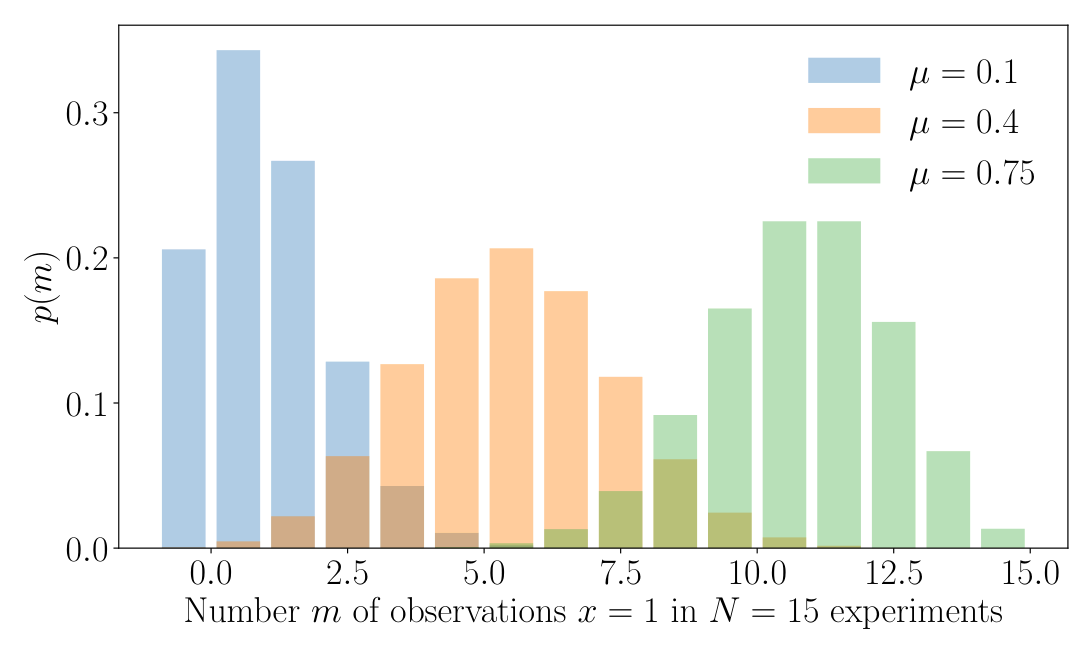
\includegraphics[width=0.92\textwidth,keepaspectratio]{docs/images/Figure6.10.png}
\caption*{\refstepcounter{figcounter}\label{fig:6-10}图~\thefigcounter 当 μ ∈ \{0.1, 0.4, 0.75\} 且 N = 15 时的二项分布示例。}
\end{figure}


\begin{notebox}
\textbf{例 6.10（Beta 分布）}
\end{notebox}

\begin{notebox}
我们可能希望对有限区间上的连续随机变量进行建模。 \emph{Beta 分布（Beta distribution）} 是连续随机变量 $ \mu \in [0, 1] $ 上的分布，常用于表示某种二元事件的概率（例如控制伯努利分布的参数）。Beta 分布 $ \mathrm{Beta}(\alpha, \beta) $ 本身（如图~\ref{fig:6-11} 所示）由两个参数 $ \alpha > 0, \beta > 0 $ 控制，定义为：

\begin{equation}
p(\mu \mid \alpha, \beta) = \frac{\Gamma(\alpha + \beta)}{\Gamma(\alpha)\Gamma(\beta)} \mu^{\alpha-1} (1 - \mu)^{\beta-1}
\tag{6.98}\label{eq:6-98}
\end{equation}

\begin{equation}
\mathbb{E}[\mu] = \frac{\alpha}{\alpha + \beta}, \quad \mathbb{V}[\mu] = \frac{\alpha\beta}{(\alpha + \beta)^2(\alpha + \beta + 1)}
\tag{6.99}\label{eq:6-99}
\end{equation}

其中 $ \Gamma(\cdot) $ 是 Gamma 函数，定义为：

\begin{equation}
\Gamma(t) := \int_0^\infty x^{t-1} \exp(-x)\,\mathrm{d}x, \quad t > 0
\tag{6.100}\label{eq:6-100}
\end{equation}

\begin{equation}
\Gamma(t + 1) = t\Gamma(t)
\tag{6.101}\label{eq:6-101}
\end{equation}

注意式~\eqref{eq:6-98} 中的 Gamma 函数分式起到了对 Beta 分布进行归一化的作用。
\end{notebox}


\begin{figure}[H]
\centering
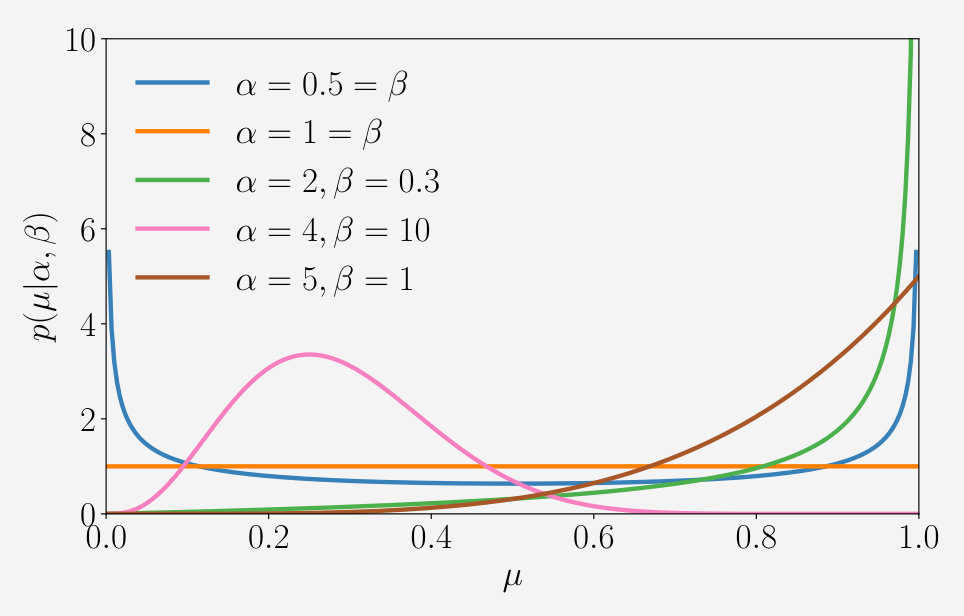
\includegraphics[width=0.92\textwidth,keepaspectratio]{docs/images/Figure6.11.png}
\caption*{\refstepcounter{figcounter}\label{fig:6-11}图~\thefigcounter α 和 β 取不同值时的 Beta 分布示例。}
\end{figure}


直观地说，$ \alpha $ 将概率质量推向 1，而 $ \beta $ 将概率质量推向 0。存在一些特殊情形 (Murphy, 2012)：

\begin{itemize}
\item 当 $ \alpha = 1 = \beta $ 时，我们得到均匀分布 $ \mathcal{U}[0, 1] $。
\item 当 $ \alpha, \beta < 1 $ 时，我们得到在 0 和 1 处有尖峰的双峰分布。
\item 当 $ \alpha, \beta > 1 $ 时，该分布是单峰的。
\item 当 $ \alpha, \beta > 1 $ 且 $ \alpha = \beta $ 时，该分布是单峰且对称的，并集中在区间 $ [0, 1] $ 的中心，即众数/均值位于 $ \frac{1}{2} $。
\end{itemize}

\emph{备注} 。存在一整套“有名字的”分布族，它们以不同方式相互关联 (Leemis and McQueston, 2008)。值得铭记的是，每个有名字的分布都是为了特定原因而创建的，但可能有其他应用。了解特定分布创立背后的原因，往往能使我们深入理解如何最好地使用它。我们引入前面的三个分布，是为了能够说明共轭性（第 6.6.1 节）和指数族（第 6.6.3 节）的概念。♦

\medskip\hrule\medskip

\section*{6.6.1 共轭性}
\addcontentsline{toc}{subsection}{6.6.1 共轭性}

根据贝叶斯定理 (6.23)，后验概率正比于先验概率与似然的乘积。先验的设定可能会很棘手，原因有二：首先，先验应当在我们看到任何数据之前概括我们对问题的先验知识，这往往难以描述；其次，通常不可能解析地计算后验分布。然而，存在一些在计算上十分方便的先验：共轭先验。

\textbf{定义 6.13}（共轭先验）。如果后验分布与先验分布具有相同的形式/类型，则称该先验分布关于似然函数是 \emph{共轭的（conjugate）} ，此时该先验称为 \emph{共轭先验（conjugate prior）} 。

共轭性特别方便，因为我们可以通过代数方式更新先验分布的参数来计算后验分布。

\emph{备注} 。当考虑概率分布的几何性质时，共轭先验保持了与似然相同的距离结构 (Agarwal and Daumé III, 2010)。♦

为了引入共轭先验的具体示例，我们在例 6.11 中描述了二项分布（定义在离散随机变量上）和 Beta 分布（定义在连续随机变量上）。

\begin{notebox}
\textbf{例 6.11（Beta-二项分布共轭性）}
\end{notebox}

\begin{notebox}
考虑二项随机变量 $ x \sim \mathrm{Bin}(N, \mu) $，其中

\begin{equation}
p(x \mid N, \mu) = \binom{N}{x} \mu^x (1 - \mu)^{N-x}, \quad x = 0, 1, \ldots, N
\tag{6.102}\label{eq:6-102}
\end{equation}

是在 $ N $ 次抛硬币中出现 $ x $ 次“正面”的概率，其中 $ \mu $ 是出现“正面”的概率。我们在参数 $ \mu $ 上引入一个 Beta 先验，即 $ \mu \sim \mathrm{Beta}(\alpha, \beta) $，其中

\begin{equation}
p(\mu \mid \alpha, \beta) = \frac{\Gamma(\alpha + \beta)}{\Gamma(\alpha)\Gamma(\beta)} \mu^{\alpha-1} (1 - \mu)^{\beta-1}
\tag{6.103}\label{eq:6-103}
\end{equation}

如果我们现在观测到某个结果 $ x = h $，即在 $ N $ 次抛硬币中看到 $ h $ 次正面，我们计算关于 $ \mu $ 的后验分布为：

\begin{equation}
p(\mu \mid x = h, N, \alpha, \beta) \propto p(x \mid N, \mu) p(\mu \mid \alpha, \beta)
\tag{6.104a}\label{eq:6-104a}
\end{equation}

\begin{equation}
\propto \mu^h (1 - \mu)^{(N-h)} \mu^{\alpha-1} (1 - \mu)^{\beta-1}
\tag{6.104b}\label{eq:6-104b}
\end{equation}

\begin{equation}
= \mu^{h+\alpha-1} (1 - \mu)^{(N-h)+\beta-1}
\tag{6.104c}\label{eq:6-104c}
\end{equation}

\begin{equation}
\propto \mathrm{Beta}(h + \alpha, N - h + \beta)
\tag{6.104d}\label{eq:6-104d}
\end{equation}

即后验分布与先验一样也是 Beta 分布，也就是说，Beta 先验对于二项似然函数中的参数 $ \mu $ 是共轭的。
\end{notebox}

在下面的例子中，我们将推导一个与 Beta-二项分布共轭性类似的结果。这里我们将展示 Beta 分布是伯努利分布的共轭先验。

\begin{notebox}
\textbf{例 6.12（Beta-伯努利分布共轭性）}
\end{notebox}

\begin{notebox}
设 $ x \in \{0, 1\} $ 服从参数为 $ \theta \in [0, 1] $ 的伯努利分布，即 $ p(x = 1 \mid \theta) = \theta $。这也可以表示为 $ p(x \mid \theta) = \theta^x (1 - \theta)^{1-x} $。设 $ \theta $ 服从参数为 $ \alpha, \beta $ 的 Beta 分布，即 $ p(\theta \mid \alpha, \beta) \propto \theta^{\alpha-1} (1 - \theta)^{\beta-1} $。
\end{notebox}

\begin{notebox}
将 Beta 分布与伯努利分布相乘，我们得到：

\begin{equation}
p(\theta \mid x, \alpha, \beta) = p(x \mid \theta) p(\theta \mid \alpha, \beta)
\tag{6.105a}\label{eq:6-105a}
\end{equation}

\begin{equation}
\propto \theta^x (1 - \theta)^{1-x} \theta^{\alpha-1} (1 - \theta)^{\beta-1}
\tag{6.105b}\label{eq:6-105b}
\end{equation}

\begin{equation}
= \theta^{\alpha+x-1} (1 - \theta)^{\beta+(1-x)-1}
\tag{6.105c}\label{eq:6-105c}
\end{equation}

\begin{equation}
\propto p(\theta \mid \alpha + x, \beta + (1 - x))
\tag{6.105d}\label{eq:6-105d}
\end{equation}

最后一行是参数为 $ (\alpha + x, \beta + (1 - x)) $ 的 Beta 分布。
\end{notebox}

表~\ref{tab:6-2} 列出了概率建模中常用的几种标准似然函数参数的共轭先验示例。诸如多项分布、逆 Gamma 分布、逆 Wishart 分布和 Dirichlet 分布等，均可在任何统计学教材中找到，并在 Bishop (2006) 等著作中有所描述。

\begin{longtable}{>{\raggedright\arraybackslash}p{\dimexpr(\textwidth-36pt)/3\relax} >{\raggedright\arraybackslash}p{\dimexpr(\textwidth-36pt)/3\relax} >{\raggedright\arraybackslash}p{\dimexpr(\textwidth-36pt)/3\relax}}
\hline
\textbf{似然} & \textbf{共轭先验} & \textbf{后验} \\ \hline
\endhead
伯努利分布 & Beta 分布 & Beta 分布 \\ \hline
二项分布 & Beta 分布 & Beta 分布 \\ \hline
高斯分布 & 高斯分布 / 逆 Gamma 分布 & 高斯分布 / 逆 Gamma 分布 \\ \hline
高斯分布 & 高斯分布 / 逆 Wishart 分布 & 高斯分布 / 逆 Wishart 分布 \\ \hline
多项分布 & Dirichlet 分布 & Dirichlet 分布 \\ \hline
\end{longtable}

\refstepcounter{tabcounter}\label{tab:6-2}表~\thetabcounter\quad 常见似然函数的共轭先验示例。

\emph{旁注} 。Gamma 先验是单变量高斯似然中精度（方差的倒数）的共轭先验，而 Wishart 先验是多元高斯似然中精度矩阵（协方差矩阵的逆）的共轭先验。

Beta 分布是二项似然和伯努利似然中参数 $ \mu $ 的共轭先验。对于高斯似然函数，我们可以在均值上放置共轭高斯先验。高斯似然在表中出现两次的原因是我们需要区分单变量和多元情形。在单变量（标量）情形下，逆 Gamma 分布是方差的共轭先验。在多元情形下，我们使用共轭逆 Wishart 分布作为协方差矩阵的先验。Dirichlet 分布是多项似然函数的共轭先验。更多详细信息请参阅 Bishop (2006)。

\medskip\hrule\medskip

\section*{6.6.2 充分统计量}
\addcontentsline{toc}{subsection}{6.6.2 充分统计量}

回顾一下，随机变量的统计量是该随机变量的确定性函数。例如，如果 $ \boldsymbol{x} = [x_1, \ldots, x_N]^\top $ 是单变量高斯随机变量构成的向量，即 $ x_n \sim \mathcal{N}(\mu, \sigma^2) $，那么样本均值 $ \hat{\mu} = \frac{1}{N}(x_1 + \cdots + x_N) $ 就是一个统计量。Ronald Fisher 爵士发现了 \emph{充分统计量（sufficient statistics）} 的概念：即存在某些统计量，它们包含了从所考虑分布对应的数据中可以推断出的所有可用信息。换言之，充分统计量携带了对总体进行推断所需的全部信息，也就是说，它们是足以代表该分布的统计量。

对于由 $ \boldsymbol{\theta} $ 参数化的一族分布，设 $ X $ 是在未知参数 $ \boldsymbol{\theta}_0 $ 下具有分布 $ p(x \mid \boldsymbol{\theta}_0) $ 的随机变量。如果统计量向量 $ \boldsymbol{\phi}(x) $ 包含了关于 $ \boldsymbol{\theta}_0 $ 的所有可能信息，则称其为 $ \boldsymbol{\theta}_0 $ 的充分统计量。更形式化地说明“包含所有可能信息”，这意味着给定 $ \boldsymbol{\theta} $ 时 $ x $ 的概率可以分解为一个不依赖于 $ \boldsymbol{\theta} $ 的部分，以及一个仅通过 $ \boldsymbol{\phi}(x) $ 依赖于 $ \boldsymbol{\theta} $ 的部分。Fisher-Neyman 分解定理形式化了这一概念，我们在定理 6.14 中给出其表述（不附证明）。

\textbf{定理 6.14}（Fisher-Neyman）。[Lehmann and Casella (1998) 中的定理 6.5] 设 $ X $ 具有概率密度函数 $ p(x \mid \boldsymbol{\theta}) $。则统计量 $ \boldsymbol{\phi}(x) $ 对于 $ \boldsymbol{\theta} $ 是充分的，当且仅当 $ p(x \mid \boldsymbol{\theta}) $ 可以写成如下形式：

\begin{equation}
p(x \mid \boldsymbol{\theta}) = h(x) g_{\boldsymbol{\theta}}(\boldsymbol{\phi}(x))
\tag{6.106}\label{eq:6-106}
\end{equation}

其中 $ h(x) $ 是独立于 $ \boldsymbol{\theta} $ 的分布，$ g_{\boldsymbol{\theta}} $ 仅通过充分统计量 $ \boldsymbol{\phi}(x) $ 捕获对 $ \boldsymbol{\theta} $ 的所有依赖。

如果 $ p(x \mid \boldsymbol{\theta}) $ 不依赖于 $ \boldsymbol{\theta} $，那么对于任意函数 $ \boldsymbol{\phi} $，$ \boldsymbol{\phi}(x) $ 平凡地是一个充分统计量。更有趣的情形是 $ p(x \mid \boldsymbol{\theta}) $ 仅依赖于 $ \boldsymbol{\phi}(x) $ 而不依赖于 $ x $ 本身。在这种情形下，$ \boldsymbol{\phi}(x) $ 是 $ \boldsymbol{\theta} $ 的充分统计量。

在机器学习中，我们考虑来自某个分布的有限数量的样本。人们可以想象，对于简单的分布（例如例 6.8 中的伯努利分布），我们只需要少量的样本即可估计该分布的参数。我们也可以考虑相反的问题：如果我们有一组数据（来自未知分布的样本），哪种分布能给出最佳拟合？一个自然会问的问题是：随着我们观察到更多的数据，我们是否需要更多的参数 $ \boldsymbol{\theta} $ 来描述该分布？事实证明，通常情况下答案是肯定的，这在非参数统计学中得到了研究 (Wasserman, 2007)。相反的问题是考虑哪类分布具有有限维充分统计量，即描述它们所需的参数数量不会任意增加。答案就是指数族分布，将在下一节中进行介绍。

\medskip\hrule\medskip

\section*{6.6.3 指数族}
\addcontentsline{toc}{subsection}{6.6.3 指数族}

在考虑（离散或连续随机变量的）分布时，我们可以有三个可能的抽象层次。在第一层次（谱系中最具体的一端），我们有一个具有固定参数的特定具名分布，例如均值为零、方差为 1 的单变量高斯分布 $ \mathcal{N}(0, 1) $。在机器学习中，我们经常使用第二层次的抽象，即固定参数形式（单变量高斯分布）并从数据中推断参数。例如，我们假设一个具有未知均值 $ \mu $ 和未知方差 $ \sigma^2 $ 的单变量高斯分布 $ \mathcal{N}(\mu, \sigma^2) $，并使用极大似然拟合来确定最佳参数 $ (\mu, \sigma^2) $。在第 9 章考虑线性回归时，我们将看到这方面的一个示例。第三个抽象层次是考虑分布族，而在本书中，我们考虑指数族。单变量高斯分布是指数族成员的一个例子。许多广泛使用的统计模型（包括表~\ref{tab:6-2} 中的所有“具名”模型）都是指数族的成员。它们都可以统一为一个概念 (Brown, 1986)。

\emph{备注} 。简短的历史掌故：如同数学和科学中的许多概念一样，指数族是由不同的研究人员在同一时间独立发现的。在 1935–1936 年间，塔斯马尼亚的 Edwin Pitman、巴黎的 Georges Darmois 以及纽约的 Bernard Koopman 独立证明了：在重复独立抽样下，指数族是唯一享有有限维充分统计量的分布族 (Lehmann and Casella, 1998)。♦

由 $ \boldsymbol{\theta} \in \mathbb{R}^D $ 参数化的 \emph{指数族（exponential family）} 是一族具有如下形式的概率分布：

\begin{equation}
p(\boldsymbol{x} \mid \boldsymbol{\theta}) = h(\boldsymbol{x}) \exp \left( \langle \boldsymbol{\theta}, \boldsymbol{\phi}(\boldsymbol{x}) \rangle - A(\boldsymbol{\theta}) \right)
\tag{6.107}\label{eq:6-107}
\end{equation}

其中 $ \boldsymbol{\phi}(\boldsymbol{x}) $ 是充分统计量向量。通常，式~\eqref{eq:6-107} 中可以使用任意内积（第 3.2 节），为了具体起见，我们在此使用标准点积（$ \langle \boldsymbol{\theta}, \boldsymbol{\phi}(\boldsymbol{x}) \rangle = \boldsymbol{\theta}^\top \boldsymbol{\phi}(\boldsymbol{x}) $）。注意，指数族的形式本质上是 Fisher-Neyman 定理（定理 6.14）中 $ g_{\boldsymbol{\theta}}(\boldsymbol{\phi}(\boldsymbol{x})) $ 的一种特定表达形式。

通过在充分统计量向量 $ \boldsymbol{\phi}(\boldsymbol{x}) $ 中添加另一项（$ \log h(\boldsymbol{x}) $），并约束对应的参数 $ \theta_0 = 1 $，因子 $ h(\boldsymbol{x}) $ 可以被吸收到点积项中。项 $ A(\boldsymbol{\theta}) $ 是确保分布求和或积分为 1 的归一化常数，称为 \emph{对数配分函数（log-partition function）} 。忽略这两项并将指数族视为具有如下形式的分布，可以获得对指数族良好的直观理解：

\begin{equation}
p(\boldsymbol{x} \mid \boldsymbol{\theta}) \propto \exp \left( \boldsymbol{\theta}^\top \boldsymbol{\phi}(\boldsymbol{x}) \right)
\tag{6.108}\label{eq:6-108}
\end{equation}

对于这种参数化形式，参数 $ \boldsymbol{\theta} $ 称为 \emph{自然参数（natural parameters）} 。乍一看，指数族似乎只是在点积结果上加上指数函数的一种平淡无奇的变换。然而，基于我们可以将有关数据的信息捕获在 $ \boldsymbol{\phi}(\boldsymbol{x}) $ 中这一事实，它带来了许多便于建模和高效计算的深远意义。

\begin{notebox}
\textbf{例 6.13（作为指数族的高斯分布）}
\end{notebox}

\begin{notebox}
考虑单变量高斯分布 $ \mathcal{N}(\mu, \sigma^2) $。令

\begin{equation*}
\boldsymbol{\phi}(x) = \begin{bmatrix} x \\ x^2 \end{bmatrix}
\end{equation*}

。利用指数族的定义，

\begin{equation}
p(x \mid \boldsymbol{\theta}) \propto \exp(\theta_1 x + \theta_2 x^2)
\tag{6.109}\label{eq:6-109}
\end{equation}

令

\begin{equation}
\boldsymbol{\theta} = \begin{bmatrix} \frac{\mu}{\sigma^2} \\ -\frac{1}{2\sigma^2} \end{bmatrix}
\tag{6.110}\label{eq:6-110}
\end{equation}

代入式~\eqref{eq:6-109}，可得：

\begin{equation}
p(x \mid \boldsymbol{\theta}) \propto \exp \left( \frac{\mu x}{\sigma^2} - \frac{x^2}{2\sigma^2} \right) \propto \exp \left( -\frac{1}{2\sigma^2} (x - \mu)^2 \right)
\tag{6.111}\label{eq:6-111}
\end{equation}

因此，单变量高斯分布是指数族的成员，其充分统计量为

\begin{equation*}
\boldsymbol{\phi}(x) = \begin{bmatrix} x \\ x^2 \end{bmatrix}
\end{equation*}

，自然参数由式~\eqref{eq:6-110} 中的 $ \boldsymbol{\theta} $ 给出。
\end{notebox}

\begin{notebox}
\textbf{例 6.14（作为指数族的伯努利分布）}
\end{notebox}

\begin{notebox}
回顾例 6.8 中的伯努利分布：

\begin{equation}
p(x \mid \mu) = \mu^x (1 - \mu)^{1-x}, \quad x \in \{0, 1\}
\tag{6.112}\label{eq:6-112}
\end{equation}

这可以写成指数族形式：

\begin{equation}
p(x \mid \mu) = \exp \left( \log \left( \mu^x (1 - \mu)^{1-x} \right) \right)
\tag{6.113a}\label{eq:6-113a}
\end{equation}

\begin{equation}
= \exp [x \log \mu + (1 - x) \log(1 - \mu)]
\tag{6.113b}\label{eq:6-113b}
\end{equation}

\begin{equation}
= \exp [x \log \mu - x \log(1 - \mu) + \log(1 - \mu)]
\tag{6.113c}\label{eq:6-113c}
\end{equation}

\begin{equation}
= \exp \left[ x \log \frac{\mu}{1 - \mu} + \log(1 - \mu) \right]
\tag{6.113d}\label{eq:6-113d}
\end{equation}

通过观察以下对应关系，最后一行 (6.113d) 可以被识别为指数族形式~\eqref{eq:6-107}：

\begin{equation}
h(x) = 1
\tag{6.114}\label{eq:6-114}
\end{equation}

\begin{equation}
\theta = \log \frac{\mu}{1 - \mu}
\tag{6.115}\label{eq:6-115}
\end{equation}

\begin{equation}
\phi(x) = x
\tag{6.116}\label{eq:6-116}
\end{equation}

\begin{equation}
A(\theta) = -\log(1 - \mu) = \log(1 + \exp(\theta))
\tag{6.117}\label{eq:6-117}
\end{equation}

$ \theta $ 与 $ \mu $ 之间的关系是可逆的，使得：

\begin{equation}
\mu = \frac{1}{1 + \exp(-\theta)}
\tag{6.118}\label{eq:6-118}
\end{equation}

式~\eqref{eq:6-118} 的关系用于获得式~\eqref{eq:6-117} 最右侧的等式。
\end{notebox}

\emph{备注} 。原始伯努利参数 $ \mu $ 与自然参数 $ \theta $ 之间的关系被称为 \emph{Sigmoid 函数（sigmoid function）} 或 \emph{Logistic 函数（logistic function）} 。观察到 $ \mu \in (0, 1) $ 但 $ \theta \in \mathbb{R} $，因此 Sigmoid 函数将实数值压缩到区间 $ (0, 1) $ 内。这一性质在机器学习中非常有用，例如它被用于 Logistic 回归（Bishop, 2006，第 4.3.2 节），以及作为神经网络中的非线性激活函数（Goodfellow et al., 2016，第 6 章）。♦

通常情况下，如何找到某个特定分布（例如表~\ref{tab:6-2} 中的分布）的共轭分布的参数形式并不显而易见。指数族提供了一种寻找共轭分布对的便捷途径。考虑随机变量 $ X $ 是指数族 (6.107) 的成员：

\begin{equation}
p(x \mid \boldsymbol{\theta}) = h(x) \exp (\langle \boldsymbol{\theta}, \boldsymbol{\phi}(x) \rangle - A(\boldsymbol{\theta}))
\tag{6.119}\label{eq:6-119}
\end{equation}

指数族的每个成员都有一个共轭先验 (Brown, 1986)：

\begin{equation}
\begin{adjustbox}{max width=\linewidth}
p(\boldsymbol{\theta} \mid \boldsymbol{\gamma}) = h_c(\boldsymbol{\theta}) \exp \left( \left\langle \begin{bmatrix} \boldsymbol{\gamma}_1 \\ \gamma_2 \end{bmatrix}, \begin{bmatrix} \boldsymbol{\theta} \\ -A(\boldsymbol{\theta}) \end{bmatrix} \right\rangle - A_c(\boldsymbol{\gamma}) \right)
\end{adjustbox}
\tag{6.120}\label{eq:6-120}
\end{equation}

其中

\begin{equation*}
\boldsymbol{\gamma} = \begin{bmatrix} \boldsymbol{\gamma}_1 \\ \gamma_2 \end{bmatrix}
\end{equation*}

的维度为 $ \mathrm{dim}(\boldsymbol{\theta}) + 1 $。共轭先验的充分统计量为

\begin{equation*}
\begin{bmatrix} \boldsymbol{\theta} \\ -A(\boldsymbol{\theta}) \end{bmatrix}
\end{equation*}

。利用指数族共轭先验通用形式的知识，我们可以推导出对应于特定分布的共轭先验函数形式。

\begin{notebox}
\textbf{例 6.15}
\end{notebox}

\begin{notebox}
回顾伯努利分布的指数族形式~\eqref{eq:6-113d}：

\begin{equation}
p(x \mid \mu) = \exp \left( x \log \frac{\mu}{1 - \mu} + \log(1 - \mu) \right)
\tag{6.121}\label{eq:6-121}
\end{equation}

其标准共轭先验的形式为：

\begin{equation}
p(\mu \mid \alpha, \beta) = \frac{\mu}{1 - \mu} \exp \left( \alpha \log \frac{\mu}{1 - \mu} + (\beta + \alpha) \log(1 - \mu) - A_c(\boldsymbol{\gamma}) \right)
\tag{6.122}\label{eq:6-122}
\end{equation}

其中我们定义了 $ \boldsymbol{\gamma} := [\alpha, \beta + \alpha]^\top $ 以及 $ h_c(\mu) := \mu / (1 - \mu) $。式~\eqref{eq:6-122} 随后可化简为：

\begin{equation}
p(\mu \mid \alpha, \beta) = \exp \left[ (\alpha - 1) \log \mu + (\beta - 1) \log(1 - \mu) - A_c(\alpha, \beta) \right]
\tag{6.123}\label{eq:6-123}
\end{equation}

将其转化为非指数族形式，得到：

\begin{equation}
p(\mu \mid \alpha, \beta) \propto \mu^{\alpha - 1} (1 - \mu)^{\beta - 1}
\tag{6.124}\label{eq:6-124}
\end{equation}

我们可将其识别为 Beta 分布 (6.98)。在例 6.12 中，我们假设了 Beta 分布是伯努利分布的共轭先验，并证明了它确实是共轭先验。而在本例中，我们通过考察伯努利分布在指数族形式下的标准共轭先验，推导出了 Beta 分布的形式。
\end{notebox}

如前一节所述，引入指数族的主要动机在于它们拥有有限维的充分统计量。此外，共轭分布易于写出，且共轭分布同样来自指数族。从推断的角度来看，极大似然估计表现良好，因为充分统计量的经验估计正是充分统计量总体值的最优估计（回顾高斯分布的均值和协方差）。从优化的角度来看，对数似然函数是凹的，从而可以使用高效的优化方法（第 7 章）。

\section*{6.7 变量替换 / 逆变换}
\addcontentsline{toc}{section}{6.7 变量替换 / 逆变换}
\label{sec:6.7}

表面上看，已知的概率分布似乎非常多，但实际上我们能叫出名字的分布集合是相当有限的。因此，了解变换后的随机变量如何分布往往非常有用。例如，假设 $ X $ 是服从单变量正态分布 $ \mathcal{N}(0, 1) $ 的随机变量，那么 $ X^2 $ 的分布是什么？另一个在机器学习中非常常见的例子是：已知 $ X_1 $ 和 $ X_2 $ 是单变量标准正态随机变量，那么 $ \frac{1}{2}(X_1 + X_2) $ 的分布是什么？

推导 $ \frac{1}{2}(X_1 + X_2) $ 分布的一种选择是计算 $ X_1 $ 和 $ X_2 $ 的均值和方差，然后将它们组合起来。正如我们在第 6.4.4 节中所见，当我们考虑随机变量的仿射变换时，可以计算所得随机变量的均值和方差。然而，在变换下我们可能无法获得分布的函数形式。此外，我们可能对随机变量的非线性变换感兴趣，而这些非线性变换的闭式表达式往往不易直接获得。

\emph{备注（符号说明）} 。在本节中，我们将明确区分随机变量及其所取的值。因此，请回顾我们使用大写字母 $ X, Y $ 表示随机变量，使用小写字母 $ x, y $ 表示随机变量在目标空间 $ \mathcal{T} $ 中所取的值。我们将离散随机变量 $ X $ 的概率质量函数（pmf）明确写作 $ P(X = x) $。对于连续随机变量 $ X $（第 6.2.2 节），概率密度函数（pdf）写作 $ f(x) $，累积分布函数（cdf）写作 $ F_X(x) $。♦

我们将探讨获取随机变量变换后分布的两种方法：一种是利用累积分布函数定义的直接方法，另一种是利用微积分链式法则（第 5.2.2 节）的变量替换方法。 \emph{矩母函数（moment generating functions）} 也可以用来研究随机变量的变换 (Casella and Berger, 2002，第 2 章)。变量替换方法被广泛使用，因为它为尝试计算变换产生的分布提供了一种标准“流程”。我们将针对单变量随机变量解释这些技术，并简要给出多元随机变量一般情形的结果。

离散随机变量的变换可以直接理解。假设存在一个离散随机变量 $ X $，其概率质量函数为 $ P(X = x) $（第 6.2.1 节），以及一个可逆函数 $ U(x) $。考虑变换后的随机变量 $ Y := U(X) $，其概率质量函数为 $ P(Y = y) $。则：

\begin{equation}
P(Y = y) = P(U(X) = y) \quad (\textcn{感兴趣的变换})
\tag{6.125a}\label{eq:6-125a}
\end{equation}

\begin{equation}
= P(X = U^{-1}(y)) \quad (\textcn{逆变换})
\tag{6.125b}\label{eq:6-125b}
\end{equation}

其中我们可以观察到 $ x = U^{-1}(y) $。因此，对于离散随机变量，变换直接改变了单个事件（其概率进行了相应变换）。

\medskip\hrule\medskip

\section*{6.7.1 分布函数法}
\addcontentsline{toc}{subsection}{6.7.1 分布函数法}

分布函数法回归到第一性原理，利用累积分布函数的定义 $ F_X(x) = P(X \leqslant x) $ 以及其导数为概率密度函数 $ f(x) $ 的事实 (Wasserman, 2004，第 2 章)。对于随机变量 $ X $ 和函数 $ U $，我们通过以下步骤求随机变量 $ Y := U(X) $ 的概率密度函数：

\begin{enumerate}
\item 求累积分布函数：
\end{enumerate}

\begin{equation}
F_Y(y) = P(Y \leqslant y)
\tag{6.126}\label{eq:6-126}
\end{equation}

\begin{enumerate}
\item 对累积分布函数 $ F_Y(y) $ 求导以获得概率密度函数 $ f(y) $：
\end{enumerate}

\begin{equation}
f(y) = \frac{\mathrm{d}}{\mathrm{d}y} F_Y(y)
\tag{6.127}\label{eq:6-127}
\end{equation}

我们还需要记住，由于 $ U $ 的变换，随机变量的定义域可能已经发生了改变。

\begin{notebox}
\textbf{例 6.16}
\end{notebox}

\begin{notebox}
设 $ X $ 为连续随机变量，在 $ 0 \leqslant x \leqslant 1 $ 上的概率密度函数为：

\begin{equation}
f(x) = 3x^2
\tag{6.128}\label{eq:6-128}
\end{equation}

我们感兴趣的是求解 $ Y = X^2 $ 的概率密度函数。
\end{notebox}

\begin{notebox}
函数 $ f $ 是 $ x $ 的递增函数，因此所得的 $ y $ 值位于区间 $ [0, 1] $ 内。我们得到：

\begin{equation}
F_Y(y) = P(Y \leqslant y) \quad (\textcn{cdf 的定义})
\tag{6.129a}\label{eq:6-129a}
\end{equation}

\begin{equation}
= P(X^2 \leqslant y) \quad (\textcn{感兴趣的变换})
\tag{6.129b}\label{eq:6-129b}
\end{equation}

\begin{equation}
= P(X \leqslant y^{\frac{1}{2}}) \quad (\textcn{逆运算})
\tag{6.129c}\label{eq:6-129c}
\end{equation}

\begin{equation}
= F_X(y^{\frac{1}{2}}) \quad (\textcn{cdf 的定义})
\tag{6.129d}\label{eq:6-129d}
\end{equation}

\begin{equation}
= \int_0^{y^{\frac{1}{2}}} 3t^2\,\mathrm{d}t \quad (\textcn{cdf 表示为定积分})
\tag{6.129e}\label{eq:6-129e}
\end{equation}

\begin{equation}
= \left[ t^3 \right]_{t=0}^{t=y^{\frac{1}{2}}} \quad (\textcn{积分结果})
\tag{6.129f}\label{eq:6-129f}
\end{equation}

\begin{equation}
= y^{\frac{3}{2}}, \quad 0 \leqslant y \leqslant 1
\tag{6.129g}\label{eq:6-129g}
\end{equation}

因此，$ Y $ 的累积分布函数为：

\begin{equation}
F_Y(y) = y^{\frac{3}{2}}
\tag{6.130}\label{eq:6-130}
\end{equation}

其中 $ 0 \leqslant y \leqslant 1 $。为了获得概率密度函数，我们对累积分布函数求导：

\begin{equation}
f(y) = \frac{\mathrm{d}}{\mathrm{d}y} F_Y(y) = \frac{3}{2} y^{\frac{1}{2}}
\tag{6.131}\label{eq:6-131}
\end{equation}

其中 $ 0 \leqslant y \leqslant 1 $。
\end{notebox}

在例 6.16 中，我们考虑了一个严格单调递增的函数 $ f(x) = 3x^2 $。这意味着我们可以计算其反函数。具有反函数的函数称为 \emph{双射函数（bijective functions）} （第 2.7 节）。一般而言，我们要求感兴趣的函数 $ y = U(x) $ 具有反函数 $ x = U^{-1}(y) $。通过考虑随机变量 $ X $ 的累积分布函数 $ F_X(x) $ 并将其用作变换 $ U(x) $，可以获得一个有用的结果。这就引出了下面的定理。

\textbf{定理 6.15}。[Casella and Berger (2002) 中的定理 2.1.10] 设 $ X $ 为具有严格单调累积分布函数 $ F_X(x) $ 的连续随机变量。则定义的随机变量

\begin{equation}
Y := F_X(X)
\tag{6.132}\label{eq:6-132}
\end{equation}

服从均匀分布。

定理 6.15 被称为 \emph{概率积分变换（probability integral transform）} ，它被用于设计从特定分布中抽样的算法（通过变换均匀随机变量的抽样结果）(Bishop, 2006)。该算法的工作原理是：首先从均匀分布中生成一个样本，然后通过逆累积分布函数（假设其可用）对其进行变换，从而获得来自目标分布的样本。概率积分变换还用于假设检验，以检验样本是否来自特定分布 (Lehmann and Romano, 2005)。累积分布函数的输出产生均匀分布这一思想，也是 \emph{连接函数（copula）} 的基础 (Nelsen, 2006)。

\medskip\hrule\medskip

\section*{6.7.2 变量替换}
\addcontentsline{toc}{subsection}{6.7.2 变量替换}

第 6.7.1 节中的分布函数法源于第一性原理，基于累积分布函数的定义并利用了反函数、微分和积分的性质。这一基于第一性原理的论证依赖于两个事实：

\begin{enumerate}
\item 我们可以将 $ Y $ 的累积分布函数转换为关于 $ X $ 的累积分布函数的表达式。
\item 我们可以对累积分布函数求导以获得概率密度函数。
\end{enumerate}

让我们逐步分解这一推理过程，目标是理解定理 6.16 中更通用的变量替换方法。概率论中的变量替换依赖于微积分中的变量替换方法 (Tandra, 2014)。

\emph{备注} 。“变量替换（change of variables）”这个名称来源于在面对困难积分时改变积分变量的想法。对于单变量函数，我们使用积分的换元法则：

\begin{equation}
\int f(g(x)) g'(x)\,\mathrm{d}x = \int f(u)\,\mathrm{d}u, \quad \textcn{其中 } u = g(x)
\tag{6.133}\label{eq:6-133}
\end{equation}

该法则的推导基于微积分的链式法则 (5.32)，并两次应用微积分基本定理。微积分基本定理形式化了积分与微分在某种程度上互为“逆运算”的事实。通过（宽泛地）考虑方程 $ u = g(x) $ 的微小变化（微分），即把 $ \Delta u = g'(x) \Delta x $ 视为 $ u = g(x) $ 的微分，可以直观地理解该规则。通过代入 $ u = g(x) $，式~\eqref{eq:6-133} 右侧积分内部的自变量变为 $ f(g(x)) $。假设项 $ \mathrm{d}u $ 可以近似为 $ \mathrm{d}u \approx \Delta u = g'(x) \Delta x $，并且 $ \mathrm{d}x \approx \Delta x $，我们就得到了式~\eqref{eq:6-133}。♦

考虑单变量随机变量 $ X $ 以及可逆函数 $ U $，这给出了另一个随机变量 $ Y = U(X) $。我们假设随机变量 $ X $ 的状态为 $ x \in [a, b] $。根据累积分布函数的定义，我们有：

\begin{equation}
F_Y(y) = P(Y \leqslant y)
\tag{6.134}\label{eq:6-134}
\end{equation}

我们对随机变量的函数 $ U $ 感兴趣：

\begin{equation}
P(Y \leqslant y) = P(U(X) \leqslant y)
\tag{6.135}\label{eq:6-135}
\end{equation}

其中我们假设函数 $ U $ 是可逆的。区间上的可逆函数要么严格单调递增，要么严格单调递减。在 $ U $ 严格单调递增的情况下，其反函数 $ U^{-1} $ 也是严格单调递增的。通过对 $ P(U(X) \leqslant y) $ 的自变量应用反函数 $ U^{-1} $，我们得到：

\begin{equation}
P(U(X) \leqslant y) = P(U^{-1}(U(X)) \leqslant U^{-1}(y)) = P(X \leqslant U^{-1}(y))
\tag{6.136}\label{eq:6-136}
\end{equation}

式~\eqref{eq:6-136} 中最右边的项是 $ X $ 的累积分布函数的表达式。回顾根据概率密度函数定义的累积分布函数：

\begin{equation}
P(X \leqslant U^{-1}(y)) = \int_a^{U^{-1}(y)} f(x)\,\mathrm{d}x
\tag{6.137}\label{eq:6-137}
\end{equation}

现在我们得到了用 $ x $ 表示的 $ Y $ 的累积分布函数表达式：

\begin{equation}
F_Y(y) = \int_a^{U^{-1}(y)} f(x)\,\mathrm{d}x
\tag{6.138}\label{eq:6-138}
\end{equation}

为了获得概率密度函数，我们对式~\eqref{eq:6-138} 关于 $ y $ 求导：

\begin{equation}
f(y) = \frac{\mathrm{d}}{\mathrm{d}y} F_Y(y) = \frac{\mathrm{d}}{\mathrm{d}y} \int_a^{U^{-1}(y)} f(x)\,\mathrm{d}x
\tag{6.139}\label{eq:6-139}
\end{equation}

注意，右侧的积分是关于 $ x $ 的，但因为我们正在关于 $ y $ 求导，所以我们需要一个关于 $ y $ 的积分。特别地，我们使用式~\eqref{eq:6-133} 进行替换：

\begin{equation}
\int f(U^{-1}(y)) (U^{-1})'(y)\,\mathrm{d}y = \int f(x)\,\mathrm{d}x, \quad \textcn{其中 } x = U^{-1}(y)
\tag{6.140}\label{eq:6-140}
\end{equation}

在式~\eqref{eq:6-139} 的右侧使用式~\eqref{eq:6-140}，得到：

\begin{equation}
f(y) = \frac{\mathrm{d}}{\mathrm{d}y} \int_a^{U^{-1}(y)} f_x(U^{-1}(y)) (U^{-1})'(y)\,\mathrm{d}y
\tag{6.141}\label{eq:6-141}
\end{equation}

然后我们回顾微分是一个线性算子，并使用下标 $ x $ 来提醒自己 $ f_x(U^{-1}(y)) $ 是 $ x $ 的函数而非 $ y $ 的函数。再次调用微积分基本定理，得到：

\begin{equation}
f(y) = f_x(U^{-1}(y)) \cdot \left( \frac{\mathrm{d}}{\mathrm{d}y} U^{-1}(y) \right)
\tag{6.142}\label{eq:6-142}
\end{equation}

回顾我们之前假设了 $ U $ 是严格单调递增函数。对于递减函数，按照相同的推导，事实证明会带有一个负号。我们引入微分的绝对值，以便对递增和递减的 $ U $ 具有统一的表达式：

\begin{equation}
f(y) = f_x(U^{-1}(y)) \cdot \left| \frac{\mathrm{d}}{\mathrm{d}y} U^{-1}(y) \right|
\tag{6.143}\label{eq:6-143}
\end{equation}

这被称为 \emph{变量替换法（change-of-variable technique）} 。式~\eqref{eq:6-143} 中的项 $ \left| \frac{\mathrm{d}}{\mathrm{d}y} U^{-1}(y) \right| $ 度量了应用 $ U $ 时单位体积的变化程度（另见第 5.3 节中雅可比矩阵的定义）。

\emph{备注} 。与式~\eqref{eq:6-125b} 中的离散情形相比，我们多了一个因子 $ \left| \frac{\mathrm{d}}{\mathrm{d}y} U^{-1}(y) \right| $。连续情形需要更加小心，因为对于所有 $ y $ 都有 $ P(Y = y) = 0 $。概率密度函数 $ f(y) $ 不能描述为涉及 $ y $ 的事件的概率。♦

到目前为止，本节主要研究了单变量的变量替换。多元随机变量的情形与此类似，但由于绝对值不能直接用于多元函数，情况变得更加复杂。相反，我们使用雅可比矩阵的行列式。回顾式~\eqref{eq:5-58}，雅可比矩阵是偏导数构成的矩阵，非零行列式的存在表明我们可以对雅可比矩阵求逆。回顾第 4.1 节中的讨论，行列式的出现是因为我们的微分（体积微元超立方体）被雅可比矩阵变换成了平行多面体。让我们将前面的讨论总结在下面的定理中，该定理给出了多元变量替换的标准流程。

\textbf{定理 6.16}。[Billingsley (1995) 中的定理 17.2] 设 $ f(\boldsymbol{x}) $ 为多元连续随机变量 $ \boldsymbol{X} $ 的概率密度值。如果向量值函数 $ \boldsymbol{y} = U(\boldsymbol{x}) $ 在 $ \boldsymbol{x} $ 定义域内的所有取值处均可微且可逆，则对于对应的 $ \boldsymbol{y} $ 取值，$ \boldsymbol{Y} = U(\boldsymbol{X}) $ 的概率密度由下式给出：

\begin{equation}
f(\boldsymbol{y}) = f_{\boldsymbol{x}}(U^{-1}(\boldsymbol{y})) \cdot \left| \det \left( \frac{\partial}{\partial \boldsymbol{y}} U^{-1}(\boldsymbol{y}) \right) \right|
\tag{6.144}\label{eq:6-144}
\end{equation}

该定理初看令人望而生畏，但关键点在于多元随机变量的变量替换遵循与单变量变量替换相同的步骤。首先，我们需要推导逆变换，并将其代入 $ \boldsymbol{x} $ 的密度函数中；然后，我们计算雅可比矩阵的行列式，并将结果相乘。下面的例子说明了二元随机变量的情形。

\begin{notebox}
\textbf{例 6.17}
\end{notebox}

\begin{notebox}
考虑一个二元随机变量 $ \boldsymbol{X} $，其状态为

\begin{equation*}
\boldsymbol{x} = \begin{bmatrix} x_1 \\ x_2 \end{bmatrix}
\end{equation*}

，概率密度函数为：

\begin{equation}
f\left( \begin{bmatrix} x_1 \\ x_2 \end{bmatrix} \right) = \frac{1}{2\pi} \exp \left( -\frac{1}{2} \begin{bmatrix} x_1 \\ x_2 \end{bmatrix}^\top \begin{bmatrix} x_1 \\ x_2 \end{bmatrix} \right)
\tag{6.145}\label{eq:6-145}
\end{equation}

我们利用定理 6.16 中的变量替换技术推导该随机变量线性变换（第 2.7 节）的影响。
\end{notebox}

\begin{notebox}
考虑矩阵 $ \boldsymbol{A} \in \mathbb{R}^{2 \times 2} $ 定义为：

\begin{equation}
\boldsymbol{A} = \begin{bmatrix} a & b \\ c & d \end{bmatrix}
\tag{6.146}\label{eq:6-146}
\end{equation}

我们感兴趣的是求解变换后的二元随机变量 $ \boldsymbol{Y} $（其状态为 $ \boldsymbol{y} = \boldsymbol{A} \boldsymbol{x} $）的概率密度函数。
\end{notebox}

\begin{notebox}
回顾变量替换需要将 $ \boldsymbol{x} $ 表示为 $ \boldsymbol{y} $ 函数的逆变换。因为我们考虑的是线性变换，逆变换由矩阵逆给出（见第 2.2.2 节）。对于 $ 2 \times 2 $ 矩阵，我们可以明确写出公式：

\begin{equation}
\begin{bmatrix} x_1 \\ x_2 \end{bmatrix} = \boldsymbol{A}^{-1} \begin{bmatrix} y_1 \\ y_2 \end{bmatrix} = \frac{1}{ad - bc} \begin{bmatrix} d & -b \\ -c & a \end{bmatrix} \begin{bmatrix} y_1 \\ y_2 \end{bmatrix}
\tag{6.147}\label{eq:6-147}
\end{equation}

观察到 $ ad - bc $ 是 $ \boldsymbol{A} $ 的行列式（第 4.1 节）。对应的概率密度函数由下式给出：

\begin{equation}
f(\boldsymbol{x}) = f(\boldsymbol{A}^{-1}\boldsymbol{y}) = \frac{1}{2\pi} \exp \left( -\frac{1}{2} \boldsymbol{y}^\top \boldsymbol{A}^{-\top} \boldsymbol{A}^{-1} \boldsymbol{y} \right)
\tag{6.148}\label{eq:6-148}
\end{equation}

矩阵乘以向量关于该向量的偏导数就是矩阵本身（第 5.5 节），因此：

\begin{equation}
\frac{\partial}{\partial \boldsymbol{y}} \boldsymbol{A}^{-1}\boldsymbol{y} = \boldsymbol{A}^{-1}
\tag{6.149}\label{eq:6-149}
\end{equation}

回顾第 4.1 节，逆矩阵的行列式等于行列式的倒数，因此雅可比矩阵的行列式为：

\begin{equation}
\det \left( \frac{\partial}{\partial \boldsymbol{y}} \boldsymbol{A}^{-1}\boldsymbol{y} \right) = \frac{1}{ad - bc}
\tag{6.150}\label{eq:6-150}
\end{equation}

现在我们可以将式~\eqref{eq:6-148} 与式~\eqref{eq:6-150} 相乘，从而应用定理 6.16 中的变量替换公式，得到：

\begin{equation}
f(\boldsymbol{y}) = f(\boldsymbol{x}) \left| \det \left( \frac{\partial}{\partial \boldsymbol{y}} \boldsymbol{A}^{-1}\boldsymbol{y} \right) \right|
\tag{6.151a}\label{eq:6-151a}
\end{equation}

\begin{equation}
= \frac{1}{2\pi} \exp \left( -\frac{1}{2} \boldsymbol{y}^\top \boldsymbol{A}^{-\top} \boldsymbol{A}^{-1} \boldsymbol{y} \right) |ad - bc|^{-1}
\tag{6.151b}\label{eq:6-151b}
\end{equation}
\end{notebox}

虽然例 6.17 基于二元随机变量（这使我们能够轻松计算矩阵逆），但上述关系对于更高维度同样成立。

\emph{备注} 。我们在第 6.5 节中看到，式~\eqref{eq:6-148} 中的密度 $ f(\boldsymbol{x}) $ 实际上是标准高斯分布，而变换后的密度 $ f(\boldsymbol{y}) $ 是协方差为 $ \boldsymbol{\Sigma} = \boldsymbol{A} \boldsymbol{A}^\top $ 的二元高斯分布。♦

我们将使用本章的思想在第 8.4 节中描述概率建模，并在第 8.5 节中引入图模型语言。我们将在第 9 章和第 11 章中看到这些思想在机器学习中的直接应用。

\section*{6.8 延伸阅读}
\addcontentsline{toc}{section}{6.8 延伸阅读}
\label{sec:6.8}

本章在某些地方写得相当简练。Grinstead and Snell (1997) 以及 Walpole et al. (2011) 提供了更为详尽且适合自学的阐述。对概率论哲学层面更感兴趣的读者可以参阅 Hacking (2001)，而 Downey (2014) 则提供了一种与软件工程联系更为紧密的方法。关于指数族的综述可参阅 Barndorff-Nielsen (2014)。在第 8 章中，我们将进一步了解如何使用概率分布对机器学习任务进行建模。具有讽刺意味的是，近期对神经网络的兴趣高涨反而促使人们对概率模型有了更广泛的认识。例如， \emph{规范化流（normalizing flows）} 的思想 (Jimenez Rezende and Mohamed, 2015) 正是依赖于变量替换来进行随机变量变换。Goodfellow et al. (2016) 一书中的第 16 章至第 20 章概述了应用于神经网络的变分推断方法。

我们通过避开测度论问题 (Billingsley, 1995; Pollard, 2002)，并且不加构造地假设实数的存在、实数上集合的定义方式及其发生的相应频率，从而避开了连续随机变量的大部分困难。这些细节确实至关重要，例如，在连续随机变量 $ x, y $ 的条件概率 $ p(y \mid x) $ 的具体规范中 (Proschan and Presnell, 1998)。简略的记号掩盖了我们想要指定 $ X = x $（这是一个测度为零的集合）的事实。此外，我们感兴趣的是 $ y $ 的概率密度函数。更精确的符号需要写为 $ \mathbb{E}_y[f(y) \mid \sigma(x)] $，其中我们对测试函数 $ f $ 在给定 $ x $ 的 $ \sigma $-代数条件下关于 $ y $ 取期望。对概率论细节感兴趣且具备更多数学背景的读者有许多选择 (Jaynes, 2003; MacKay, 2003; Jacod and Protter, 2004; Grimmett and Welsh, 2014)，包括一些非常深入的技术性讨论 (Shiryayev, 1984; Lehmann and Casella, 1998; Dudley, 2002; Bickel and Doksum, 2006; Çınlar, 2011)。另一种研究概率的方法是从期望的概念出发，然后“逆向推导”出概率空间的必要性质 (Whittle, 2000)。随着机器学习使我们能够对越来越复杂的数据类型上的更错综复杂的分布进行建模，概率机器学习模型的开发者必须理解这些更为技术的层面。侧重于概率建模的机器学习教材包括 MacKay (2003)、Bishop (2006)、Rasmussen and Williams (2006)、Barber (2012) 以及 Murphy (2012) 的著作。

\chapter*{练习}
\addcontentsline{toc}{section}{练习}

\section*{练习 7.1}
\addcontentsline{toc}{subsection}{练习 7.1}

考虑单变量函数：

\begin{equation*}
f(x) = x^3 + 6x^2 - 3x - 5
\end{equation*}

求其驻点，并指出它们是极大值点、极小值点还是鞍点。

\medskip\hrule\medskip

\section*{练习 7.2}
\addcontentsline{toc}{subsection}{练习 7.2}

考虑随机梯度下降的更新方程（式~\eqref{eq:7-15}）。写出当我们使用大小为 1 的小批量（mini-batch）时的更新公式。

\medskip\hrule\medskip

\section*{练习 7.3}
\addcontentsline{toc}{subsection}{练习 7.3}

判断下列陈述的真伪： a. 任意两个凸集的交集是凸集。 b. 任意两个凸集的并集是凸集。 c. 一个凸集 $ A $ 与另一个凸集 $ B $ 的差集是凸集。

\medskip\hrule\medskip

\section*{练习 7.4}
\addcontentsline{toc}{subsection}{练习 7.4}

判断下列陈述的真伪： a. 任意两个凸函数之和是凸函数。 b. 任意两个凸函数之差是凸函数。 c. 任意两个凸函数之积是凸函数。 d. 任意两个凸函数的逐点最大值是凸函数。

\medskip\hrule\medskip

\section*{练习 7.5}
\addcontentsline{toc}{subsection}{练习 7.5}

将以下优化问题用矩阵记号表示为标准线性规划：

\begin{equation*}
\max_{\boldsymbol{x} \in \mathbb{R}^2,\, \xi \in \mathbb{R}} \boldsymbol{p}^\top \boldsymbol{x} + \xi
\end{equation*}

满足约束条件 $ \xi \geqslant 0 $、$ x_0 \leqslant 0 $ 且 $ x_1 \leqslant 3 $。

\medskip\hrule\medskip

\section*{练习 7.6}
\addcontentsline{toc}{subsection}{练习 7.6}

考虑图 7.9 中所示的线性规划：

\begin{equation*}
\begin{adjustbox}{max width=\linewidth}
\begin{aligned}
\min_{\boldsymbol{x} \in \mathbb{R}^2} \quad & -\begin{bmatrix} 5 \\ 3 \end{bmatrix}^\top \begin{bmatrix} x_1 \\ x_2 \end{bmatrix} \\
\text{subject to} \quad & \begin{bmatrix} 2 & 2 \\ 2 & -4 \\ -2 & 1 \\ 0 & -1 \\ 0 & 1 \end{bmatrix} \begin{bmatrix} x_1 \\ x_2 \end{bmatrix} \leqslant \begin{bmatrix} 33 \\ 8 \\ 5 \\ -1 \\ 8 \end{bmatrix}
\end{aligned}
\end{adjustbox}
\end{equation*}

利用拉格朗日对偶性推导其对偶线性规划。

\medskip\hrule\medskip

\section*{练习 7.7}
\addcontentsline{toc}{subsection}{练习 7.7}

考虑图 7.4 中所示的二次规划：

\begin{equation*}
\begin{adjustbox}{max width=\linewidth}
\begin{aligned}
\min_{\boldsymbol{x} \in \mathbb{R}^2} \quad & \frac{1}{2}\begin{bmatrix} x_1 \\ x_2 \end{bmatrix}^\top \begin{bmatrix} 2 & 1 \\ 1 & 4 \end{bmatrix} \begin{bmatrix} x_1 \\ x_2 \end{bmatrix} + \begin{bmatrix} 5 \\ 3 \end{bmatrix}^\top \begin{bmatrix} x_1 \\ x_2 \end{bmatrix} \\
\text{subject to} \quad & \begin{bmatrix} 1 & 0 \\ -1 & 0 \\ 0 & 1 \\ 0 & -1 \end{bmatrix} \begin{bmatrix} x_1 \\ x_2 \end{bmatrix} \leqslant \begin{bmatrix} 1 \\ 1 \\ 1 \\ 1 \end{bmatrix}
\end{aligned}
\end{adjustbox}
\end{equation*}

利用拉格朗日对偶性推导其对偶二次规划。

\medskip\hrule\medskip

\section*{练习 7.8}
\addcontentsline{toc}{subsection}{练习 7.8}

考虑以下凸优化问题：

\begin{equation*}
\begin{aligned}
\min_{\boldsymbol{w} \in \mathbb{R}^D} \quad & \frac{1}{2}\boldsymbol{w}^\top \boldsymbol{w} \\
\text{subject to} \quad & \boldsymbol{w}^\top \boldsymbol{x} \geqslant 1
\end{aligned}
\end{equation*}

通过引入拉格朗日乘子 $ \lambda $，推导其拉格朗日对偶问题。

\medskip\hrule\medskip

\section*{练习 7.9}
\addcontentsline{toc}{subsection}{练习 7.9}

考虑 $ \boldsymbol{x} \in \mathbb{R}^D $ 的负熵函数：

\begin{equation*}
f(\boldsymbol{x}) = \sum_{d=1}^D x_d \log x_d
\end{equation*}

假设使用标准点积，推导其凸共轭函数 $ f^*(\boldsymbol{s}) $。 提示：对适当的函数求梯度并令梯度为零。

\medskip\hrule\medskip

\section*{练习 7.10}
\addcontentsline{toc}{subsection}{练习 7.10}

考虑函数：

\begin{equation*}
f(\boldsymbol{x}) = \frac{1}{2}\boldsymbol{x}^\top \boldsymbol{A} \boldsymbol{x} + \boldsymbol{b}^\top \boldsymbol{x} + c
\end{equation*}

其中 $ \boldsymbol{A} $ 严格正定，这意味着它是可逆的。推导 $ f(\boldsymbol{x}) $ 的凸共轭函数。 提示：对适当的函数求梯度并令梯度为零。

\medskip\hrule\medskip

\section*{练习 7.11}
\addcontentsline{toc}{subsection}{练习 7.11}

合页损失（hinge loss，即支持向量机所使用的损失函数）由下式给出：

\begin{equation*}
L(\alpha) = \max\{0, 1 - \alpha\}
\end{equation*}

如果我们希望应用诸如 L-BFGS 之类的梯度方法，而不希望诉诸次梯度法，我们需要平滑合页损失中的尖折点。计算合页损失的凸共轭 $ L^*(\beta) $，其中 $ \beta $ 为对偶变量。添加一个 $ \ell_2 $ 近端项，并计算所得函数的共轭：

\begin{equation*}
L^*(\beta) + \frac{\gamma}{2}\beta^2
\end{equation*}

其中 $ \gamma $ 为给定的超参数。

\chapter{7 连续优化}

由于机器学习算法最终在计算机上实现，其数学公式通常表示为数值优化方法。本章描述了用于训练机器学习模型的基本数值方法。训练机器学习模型往往归结为寻找一组良好的参数。“良好”的概念由目标函数或概率模型决定，我们将在本书第二部分看到相关示例。给定目标函数，寻找最优值是通过优化算法完成的。

由于我们考虑的数据和模型位于 $ \mathbb{R}^D $ 中，我们面对的优化问题是 \emph{连续优化（continuous optimization）} 问题，这与针对离散变量的组合优化问题截然不同。

本章涵盖连续优化的两个主要分支（图~\ref{fig:7-1}）：无约束优化与带约束优化。在本章中，我们将假定目标函数是可微的（参见第 5 章），因此我们在空间中的每个位置都可以利用梯度来帮助我们寻找最优值。按照惯例，机器学习中的大多数目标函数都是为了最小化而设计的，即最优值就是最小值。在几何直观上，寻找最优值就像寻找目标函数的山谷底，而梯度总是指向“上坡”方向。优化的基本思想是沿着“下坡”方向（即负梯度方向）移动，以期找到最深的点。对于无约束优化，这是我们唯一需要的核心概念，但涉及到若干设计选择，我们将在第 7.1 节中进行讨论。对于带约束优化，我们需要引入其他概念来处理约束（第 7.2 节）。我们还将介绍一类特殊的问题——凸优化问题（第 7.3 节），在凸优化中我们可以确切保证找到全局最优解。


\begin{figure}[H]
\centering
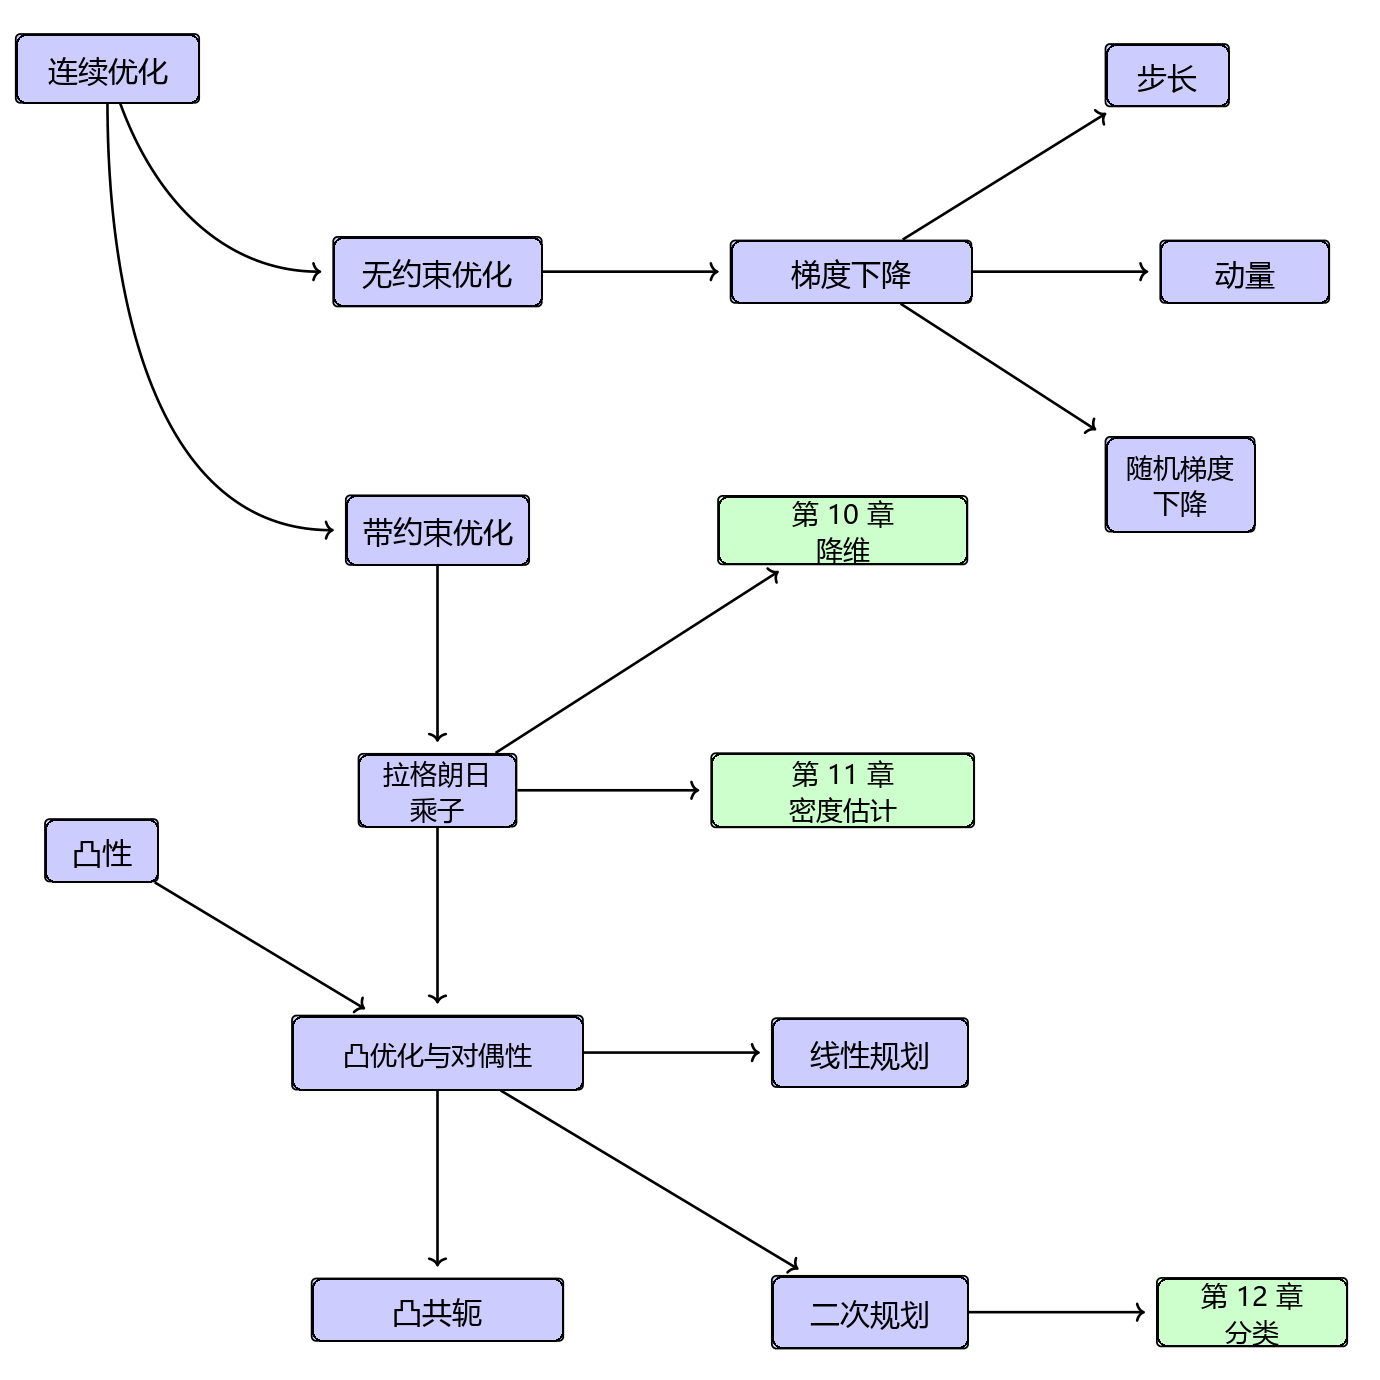
\includegraphics[width=320pt,keepaspectratio]{docs/images/Figure7.1.png}
\caption*{\refstepcounter{figcounter}\label{fig:7-1}图~\thefigcounter 本章介绍的与优化相关概念的思维导图。包含两大核心思想：梯度下降与凸优化。}
\end{figure}


考虑图~\ref{fig:7-2} 中所示的函数。该函数在 $ x \approx -4.5 $ 处具有一个全局最小值，函数值约为 $ -47 $。由于该函数是“平滑”的，梯度可以通过指明我们应该向右还是向左迈步来帮助寻找最小值。这假定我们处于正确的“碗”中，因为在 $ x \approx 0.7 $ 处还存在另一个局部最小值。回想一下，我们可以通过计算函数的导数并令其为零来求解函数的所有驻点。对于多项式函数：

\begin{equation}
\ell(x) = x^4 + 7x^3 + 5x^2 - 17x + 3
\tag{7.1}\label{eq:7-1}
\end{equation}

我们得到对应的梯度（一阶导数）为：

\begin{equation}
\frac{\mathrm{d}\ell(x)}{\mathrm{d}x} = 4x^3 + 21x^2 + 10x - 17
\tag{7.2}\label{eq:7-2}
\end{equation}

\emph{提示} ：驻点是导数的实根，即梯度为零的点。


\begin{figure}[H]
\centering
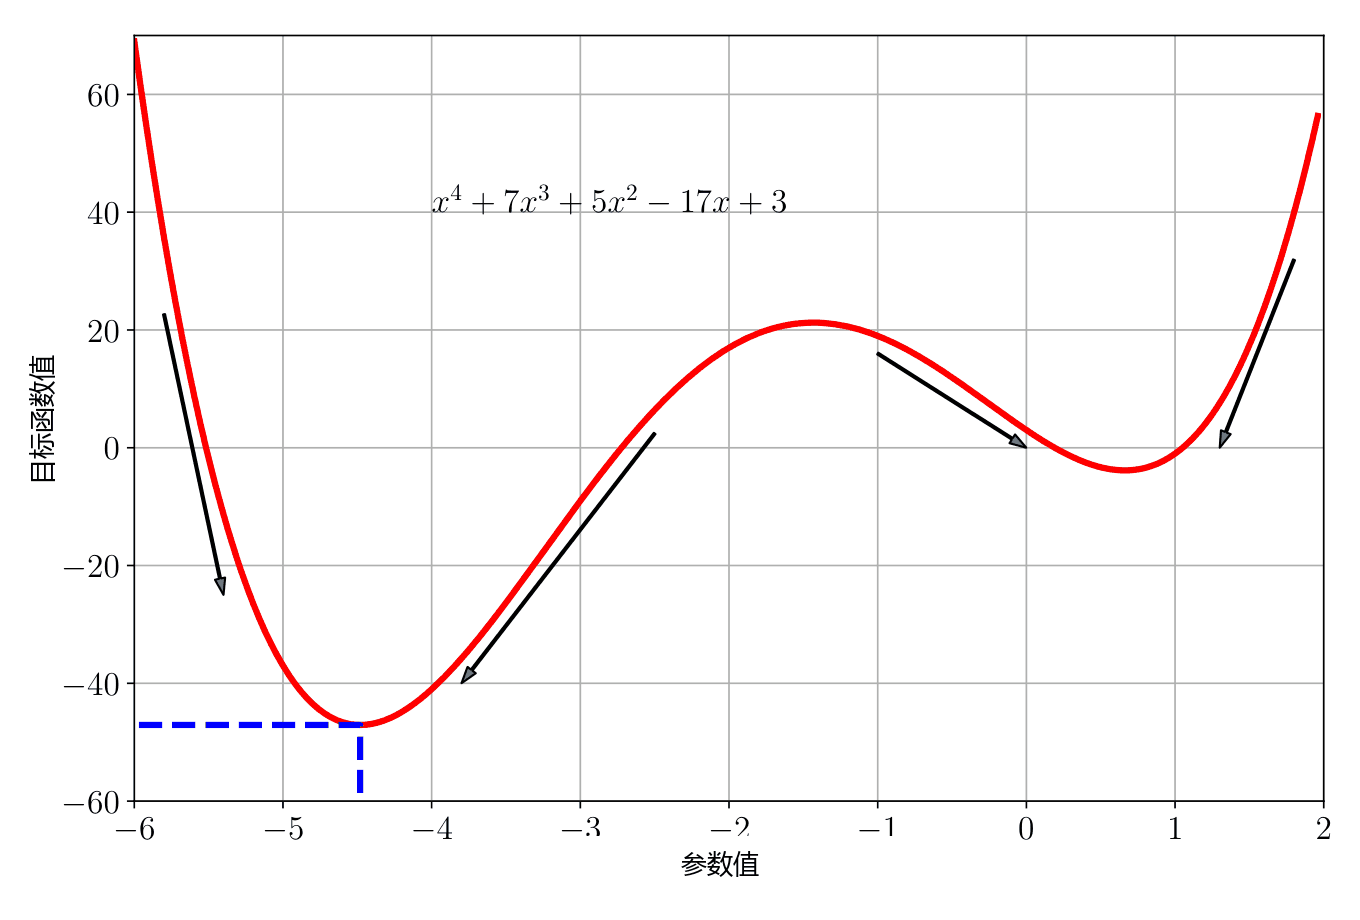
\includegraphics[width=0.92\textwidth,keepaspectratio]{docs/images/Figure7.2.png}
\caption*{\refstepcounter{figcounter}\label{fig:7-2}图~\thefigcounter 目标函数示例。负梯度方向由箭头指示，全局最小值由蓝色虚线指示。}
\end{figure}


由于式~\eqref{eq:7-2} 是一个三次方程，令其为零时通常具有三个解。在示例中，其中两个是极小值点，一个是极大值点（在 $ x \approx -1.4 $ 附近）。为了检验驻点是极小值还是极大值，我们需要求二阶导数，并检验驻点处的二阶导数是正还是负。在我们的情形中，二阶导数为：

\begin{equation}
\frac{\mathrm{d}^2\ell(x)}{\mathrm{d}x^2} = 12x^2 + 42x + 10
\tag{7.3}\label{eq:7-3}
\end{equation}

将目测估计值 $ x = -4.5, -1.4, 0.7 $ 代入，我们会观察到正如预期的那样，中间点对应于极大值（$ \frac{\mathrm{d}^2\ell(x)}{\mathrm{d}x^2} < 0 $），而其他两个驻点对应于极小值。

注意到在前面的讨论中我们避免了解析求解 $ x $ 的确切值，尽管对于这类低阶多项式我们确实能够做到这一点。但在一般情况下，根据阿贝尔-鲁菲尼定理（Abel–Ruffini theorem），对于 5 次或更高阶的多项式通常不存在代数解（Abel, 1826）。在一般高维问题中我们无法找到解析解，因此需要从某个初始值（例如 $ x_0 = -6 $）出发，沿着负梯度方向进行迭代。负梯度表明我们应该向右移动，但没有指明移动多远（这称为步长）。此外，如果从右侧开始（例如 $ x_0 = 0 $），负梯度将引导我们走向错误的局部极小值。图~\ref{fig:7-2} 说明了对于 $ x > -1 $ 的情况，负梯度指向右侧的极小值，其目标函数值明显更大。

在第 7.3 节中，我们将学习一类称为凸函数的函数，这类函数不会对优化算法的起始点产生这种棘手的敏感依赖性。对于凸函数，所有局部极小值都是全局最小值。事实证明，许多机器学习目标函数都被专门设计为凸函数，我们将在第 12 章中看到具体示例。

到目前为止本章的讨论主要围绕一维函数展开，借此我们能够直观可视化梯度、下降方向和最优值等概念。在接下来的小节中，我们将把相同的思想推广到高维情形。

\section*{7.1 使用梯度下降的优化}
\addcontentsline{toc}{section}{7.1 使用梯度下降的优化}
\label{sec:7.1}

我们现在考虑求解实值函数的极小值问题：

\begin{equation}
\min_{\boldsymbol{x}} f(\boldsymbol{x})
\tag{7.4}\label{eq:7-4}
\end{equation}

其中 $ f : \mathbb{R}^d \to \mathbb{R} $ 是刻画当前机器学习问题的目标函数。我们假定函数 $ f $ 是可微的，并且无法求出解析闭式解。

\emph{梯度下降（gradient descent）} 是一种一阶优化算法。为了使用梯度下降寻找函数的局部极小值，迭代步长与函数在当前点处的负梯度成比例。回想第 5.1 节，梯度指向最陡上升的方向。另一个有用的几何直觉是考虑函数的等值线集合（对于某个常数 $ c \in \mathbb{R} $ 满足 $ f(\boldsymbol{x}) = c $ 的曲线），称为等高线。梯度方向始终与目标函数的等高线正交。

让我们考虑多元函数。想象一个由函数 $ f(\boldsymbol{x}) $ 描述的曲面，一个球从特定位置 $ \boldsymbol{x}_0 $ 开始释放。当小球被释放时，它将沿着最陡下降的方向滚下山坡。梯度下降利用了这样一个性质：如果从 $ \boldsymbol{x}_0 $ 出发沿着 $ f $ 在 $ \boldsymbol{x}_0 $ 处的负梯度方向 $ -(\nabla f(\boldsymbol{x}_0))^\top $ 移动，函数值 $ f(\boldsymbol{x}_0) $ 下降最快。在本书中，我们假定函数是可微的。那么，对于较小的步长 $ \gamma \geqslant 0 $，若：

\begin{equation}
\boldsymbol{x}_1 = \boldsymbol{x}_0 - \gamma (\nabla f(\boldsymbol{x}_0))^\top
\tag{7.5}\label{eq:7-5}
\end{equation}

则必有 $ f(\boldsymbol{x}_1) \leqslant f(\boldsymbol{x}_0) $。请注意，我们在梯度上使用了转置，因为根据本书的约定，梯度为行向量，转置后才能与列向量的维度相匹配。

这一观察使我们能够定义一个简单的梯度下降算法：如果我们希望寻找函数 $ f : \mathbb{R}^n \to \mathbb{R}, \boldsymbol{x} \mapsto f(\boldsymbol{x}) $ 的局部最优点 $ f(\boldsymbol{x}_*) $，我们从希望优化的参数的初始猜测 $ \boldsymbol{x}_0 $ 开始，然后按照如下规则迭代：

\begin{equation}
\boldsymbol{x}_{i+1} = \boldsymbol{x}_i - \gamma_i (\nabla f(\boldsymbol{x}_i))^\top
\tag{7.6}\label{eq:7-6}
\end{equation}

对于合适的步长 $ \gamma_i $，序列 $ f(\boldsymbol{x}_0) \geqslant f(\boldsymbol{x}_1) \geqslant \cdots $ 收敛至局部极小值。

\begin{notebox}
\textbf{例 7.1}
\end{notebox}

\begin{notebox}
考虑二维二次函数：

\begin{equation}
\begin{adjustbox}{max width=\linewidth}
f\left(\begin{bmatrix} x_1 \\ x_2 \end{bmatrix}\right) = \frac{1}{2} \begin{bmatrix} x_1 \\ x_2 \end{bmatrix}^\top \begin{bmatrix} 2 & 1 \\ 1 & 20 \end{bmatrix} \begin{bmatrix} x_1 \\ x_2 \end{bmatrix} - \begin{bmatrix} 5 \\ 3 \end{bmatrix}^\top \begin{bmatrix} x_1 \\ x_2 \end{bmatrix}
\end{adjustbox}
\tag{7.7}\label{eq:7-7}
\end{equation}

其梯度为：

\begin{equation}
\nabla f\left(\begin{bmatrix} x_1 \\ x_2 \end{bmatrix}\right) = \begin{bmatrix} x_1 \\ x_2 \end{bmatrix}^\top \begin{bmatrix} 2 & 1 \\ 1 & 20 \end{bmatrix} - \begin{bmatrix} 5 & 3 \end{bmatrix}
\tag{7.8}\label{eq:7-8}
\end{equation}

从初始位置 $ \boldsymbol{x}_0 = [-3, -1]^\top $ 开始，我们反复应用式~\eqref{eq:7-6} 来获得收敛到极小值的一系列估计（如图~\ref{fig:7-3} 所示）。从图中以及将 $ \boldsymbol{x}_0 $ 代入式~\eqref{eq:7-8}（取 $ \gamma = 0.085 $）都可以看出，在 $ \boldsymbol{x}_0 $ 处的负梯度指向东北方向，得到 $ \boldsymbol{x}_1 = [-1.98, 1.21]^\top $。重复这一迭代过程，我们得到 $ \boldsymbol{x}_2 = [-1.32, -0.42]^\top $，以此类推。
\end{notebox}


\begin{figure}[H]
\centering
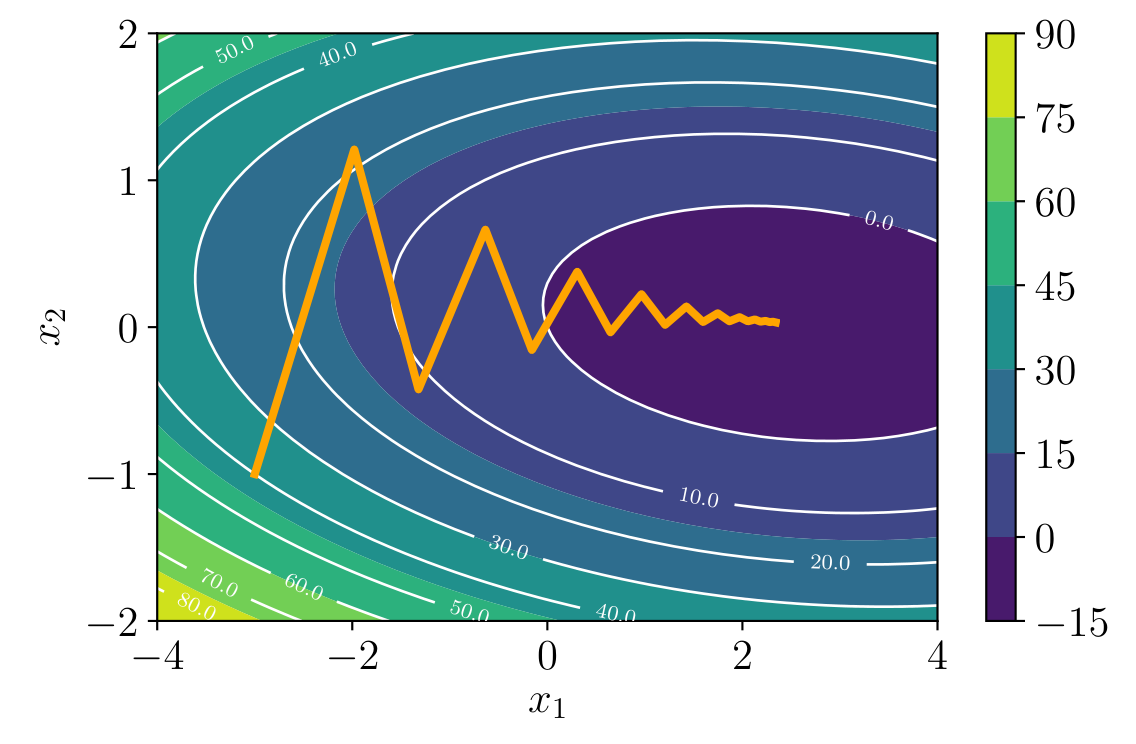
\includegraphics[width=0.92\textwidth,keepaspectratio]{docs/images/Figure7.3.png}
\caption*{\refstepcounter{figcounter}\label{fig:7-3}图~\thefigcounter 二维二次曲面上的梯度下降（以热图展示）。}
\end{figure}


\emph{备注} 。在接近极小值时，梯度下降的速度可能相对较慢：其渐近收敛速度逊色于许多其他优化方法。继续使用小球滚下山坡的比喻，当优化曲面是一个狭长的山谷时，该问题是病态的（ill-conditioned）（Trefethen and Bau III, 1997）。对于病态凸问题，随着梯度方向几乎与通往极小值点的最短路径正交，梯度下降会呈现越来越严重的“之字形”（zigzag）振荡震荡现象；参见图~\ref{fig:7-3}。♦

\medskip\hrule\medskip

\section*{7.1.1 步长}
\addcontentsline{toc}{subsection}{7.1.1 步长}

如前所述，在梯度下降中选择合适的步长至关重要。步长通常也被称为 \emph{学习率（learning rate）} 。如果步长太小，梯度下降的进展可能极其缓慢；如果步长选得过大，梯度下降可能会发生超调（overshoot），导致算法无法收敛甚至发散。我们将在下一小节讨论动量（momentum）的使用，这是一种能够平滑梯度更新的不规则跳跃并抑制震荡的有效方法。

自适应梯度方法在每次迭代时根据函数的局部性质重新缩放步长。存在两个简单的启发式准则（Toussaint, 2012）：

\begin{itemize}
\item 当单步梯度更新后函数值增加时，说明步长过大：撤销该步更新并减小步长。
\item 当函数值减少时，步长原本可以更大：尝试增加步长。
\end{itemize}

虽然“撤销”操作看似浪费了计算资源，但采用该启发式法则可以从理论上保证单调收敛。

\begin{notebox}
\textbf{例 7.2（求解线性方程组）}
\end{notebox}

\begin{notebox}
当我们求解形如 $ \boldsymbol{A} \boldsymbol{x} = \boldsymbol{b} $ 的线性方程组时，在实践中我们通过寻找使平方误差最小化的 $ \boldsymbol{x}_* $ 来近似求解：

\begin{equation}
\|\boldsymbol{A} \boldsymbol{x} - \boldsymbol{b}\|^2 = (\boldsymbol{A} \boldsymbol{x} - \boldsymbol{b})^\top (\boldsymbol{A} \boldsymbol{x} - \boldsymbol{b})
\tag{7.9}\label{eq:7-9}
\end{equation}

式~\eqref{eq:7-9} 关于 $ \boldsymbol{x} $ 的梯度为：

\begin{equation}
\nabla_{\boldsymbol{x}} = 2(\boldsymbol{A} \boldsymbol{x} - \boldsymbol{b})^\top \boldsymbol{A}
\tag{7.10}\label{eq:7-10}
\end{equation}

我们可以将此梯度直接应用于梯度下降算法中。然而，对于这个特殊的线性最小二乘情形，令梯度为零实际上可以直接解出解析闭式解。我们将在第 9 章深入讨论最小二乘问题的求解。
\end{notebox}

\emph{备注} 。当应用于线性方程组 $ \boldsymbol{A} \boldsymbol{x} = \boldsymbol{b} $ 时，梯度下降的收敛速度可能很慢。梯度下降的收敛速度取决于矩阵 $ \boldsymbol{A} $ 的 \emph{条件数（condition number）} ：

\begin{equation*}
\kappa = \frac{\sigma_{\max}(\boldsymbol{A})}{\sigma_{\min}(\boldsymbol{A})}
\end{equation*}

即 $ \boldsymbol{A} $ 的最大奇异值与最小奇异值之比（参见第 4.5 节）。条件数本质上度量了曲率最大方向与曲率最小方向的比率，这恰好对应于病态问题就像狭长山谷的比喻：它们在一个方向上高度弯曲，而在另一个方向上极其平坦。此时与其直接求解 $ \boldsymbol{A} \boldsymbol{x} = \boldsymbol{b} $，不如求解预条件方程 $ \boldsymbol{P}^{-1}(\boldsymbol{A} \boldsymbol{x} - \boldsymbol{b}) = \boldsymbol{0} $，其中 $ \boldsymbol{P} $ 称为 \emph{预条件子（preconditioner）} 。其目标是设计 $ \boldsymbol{P}^{-1} $ 使得 $ \boldsymbol{P}^{-1} \boldsymbol{A} $ 拥有显著改善的条件数，同时 $ \boldsymbol{P}^{-1} $ 易于计算。♦

\medskip\hrule\medskip

\section*{7.1.2 带动量的梯度下降}
\addcontentsline{toc}{subsection}{7.1.2 带动量的梯度下降}

如图~\ref{fig:7-3} 所示，如果优化曲面的曲率使得某些区域尺度极不均衡，梯度下降的收敛速度可能会非常缓慢。曲率导致梯度下降步在峡谷的两侧峭壁之间来回跳跃，仅以微小的步伐向极值点推进。改善收敛性的一种著名技巧是赋予梯度下降一定的“记忆能力”。

\emph{带动量的梯度下降（gradient descent with momentum）} （Rumelhart et al., 1986）引入了一个额外项来记忆前一次迭代发生的情况。这种记忆机制能够抑制振荡并平滑梯度更新轨迹。继续使用小球比喻，动量项模拟了具有较大质量的沉重铁球在滚动时不愿轻易改变行进方向的物理惯性。其思想是借助带有记忆的梯度更新来实现指数移动平均。基于动量的方法记录每次迭代 $ i $ 的更新量 $ \Delta \boldsymbol{x}_i $，并将下一次更新确定为当前梯度与先前梯度的线性组合：

\begin{equation}
\boldsymbol{x}_{i+1} = \boldsymbol{x}_i - \gamma_i (\nabla f(\boldsymbol{x}_i))^\top + \alpha \Delta \boldsymbol{x}_i
\tag{7.11}\label{eq:7-11}
\end{equation}

\begin{equation}
\Delta \boldsymbol{x}_i = \boldsymbol{x}_i - \boldsymbol{x}_{i-1} = \alpha \Delta \boldsymbol{x}_{i-1} - \gamma_{i-1} (\nabla f(\boldsymbol{x}_{i-1}))^\top
\tag{7.12}\label{eq:7-12}
\end{equation}

其中 $ \alpha \in [0, 1] $。有时我们仅能近似获知梯度，在这些情形下动量项非常有用，因为它能平均掉梯度的随机噪声估计。

\medskip\hrule\medskip

\section*{7.1.3 随机梯度下降}
\addcontentsline{toc}{subsection}{7.1.3 随机梯度下降}

精确计算整个数据集上的完整梯度可能极其耗时。然而，通常可以找到一种计算成本低廉的“廉价”梯度近似。只要近似梯度的大致方向与真实梯度一致，该近似仍然非常有效。

\emph{随机梯度下降（stochastic gradient descent, SGD）} 是一种针对表示为可微函数之和的目标函数进行最小化的随机近似优化算法。这里的“随机”是指我们承认无法精确获知真实梯度，而只掌握其带噪声的近似。通过对近似梯度的概率分布施加合理约束，我们在理论上仍然可以保证 SGD 能够收敛。

在机器学习中，给定 $ n = 1, \ldots, N $ 个数据点，我们通常考虑的目标函数是由每个样本 $ n $ 产生的损失 $ L_n $ 的累加和：

\begin{equation}
L(\boldsymbol{\theta}) = \sum_{n=1}^N L_n(\boldsymbol{\theta})
\tag{7.13}\label{eq:7-13}
\end{equation}

其中 $ \boldsymbol{\theta} $ 是我们感兴趣的参数矢量。回归问题（第 9 章）中的一个典型例子是负对数似然，它表示为各个单独样本对数似然的求和：

\begin{equation}
L(\boldsymbol{\theta}) = -\sum_{n=1}^N \log p(y_n \mid \boldsymbol{x}_n, \boldsymbol{\theta})
\tag{7.14}\label{eq:7-14}
\end{equation}

其中 $ \boldsymbol{x}_n \in \mathbb{R}^D $ 是训练输入，$ y_n $ 是训练目标，而 $ \boldsymbol{\theta} $ 是回归模型的参数。

前面介绍的标准梯度下降是一种“批量”（batch）优化方法，即每次更新都使用完整的训练集：

\begin{equation}
\boldsymbol{\theta}_{i+1} = \boldsymbol{\theta}_i - \gamma_i (\nabla L(\boldsymbol{\theta}_i))^\top = \boldsymbol{\theta}_i - \gamma_i \sum_{n=1}^N (\nabla L_n(\boldsymbol{\theta}_i))^\top
\tag{7.15}\label{eq:7-15}
\end{equation}

当训练集极其庞大时，评估全梯度的求和计算开销极为高昂。

考察式~\eqref{eq:7-15} 中的梯度和 $ \sum_{n=1}^N \nabla L_n(\boldsymbol{\theta}_i) $，我们可以通过在一个较小的 $ L_n $ 子集上求和来显著减少计算量。与使用全部 $ N $ 个样本的批量梯度下降不同，我们在 \emph{小批量梯度下降（mini-batch gradient descent）} 中随机选择一个子集；在极端情况下，我们甚至可以仅随机选择单个样本 $ L_n $ 来估计梯度。抽取数据子集之所以合理，其关键洞察在于：\textbf{为了使梯度下降收敛，我们仅要求近似梯度是真实梯度的无偏估计}。实际上，式~\eqref{eq:7-15} 中的项正是梯度期望值（第 6.4.1 节）的经验估计；因此，基于任意数据随机子样本得到的任何其他无偏经验估计，都足以保证梯度下降的收敛性。

\emph{备注} 。在学习率以合适速率衰减且满足相对温和的假设条件下，随机梯度下降几乎必然收敛至局部极小值（Bottou, 1998）。♦

采用小批量的另一个核心原因是硬件实践约束，例如 CPU/GPU 内存大小或计算时间的限制。较大的小批量（batch size）能够提供更精确的梯度估计，减小参数更新的方差，并且能充分利用向量化运算中高度优化的矩阵乘法；而较小的小批量计算速度极快，且其梯度估计中固有的噪声往往有助于算法跳出不良局部极值点。在现代大规模机器学习中，随机梯度下降已被证明极为高效（Bottou et al., 2018），广泛应用于深度神经网络、主题模型、强化学习及大规模高斯过程模型的训练。

\section*{7.2 带约束优化与拉格朗日乘子}
\addcontentsline{toc}{section}{7.2 带约束优化与拉格朗日乘子}
\label{sec:7.2}

在上一节中，我们考虑了求解函数极小值的问题：

\begin{equation}
\min_{\boldsymbol{x}} f(\boldsymbol{x})
\tag{7.16}\label{eq:7-16}
\end{equation}

其中 $ f : \mathbb{R}^D \to \mathbb{R} $。

在本节中，我们增加了额外的约束。也就是说，对于实值函数 $ g_i : \mathbb{R}^D \to \mathbb{R} $（$ i = 1, \ldots, m $），我们考虑如下带约束优化问题（见图~\ref{fig:7-4} 示意）：

\begin{equation}
\begin{aligned}
\min_{\boldsymbol{x}} & \quad f(\boldsymbol{x}) \\
\text{subject to} & \quad g_i(\boldsymbol{x}) \leqslant 0 \quad \textcn{对所有 } i = 1, \ldots, m \textcn{。}
\end{aligned}
\tag{7.17}\label{eq:7-17}
\end{equation}


\begin{figure}[H]
\centering
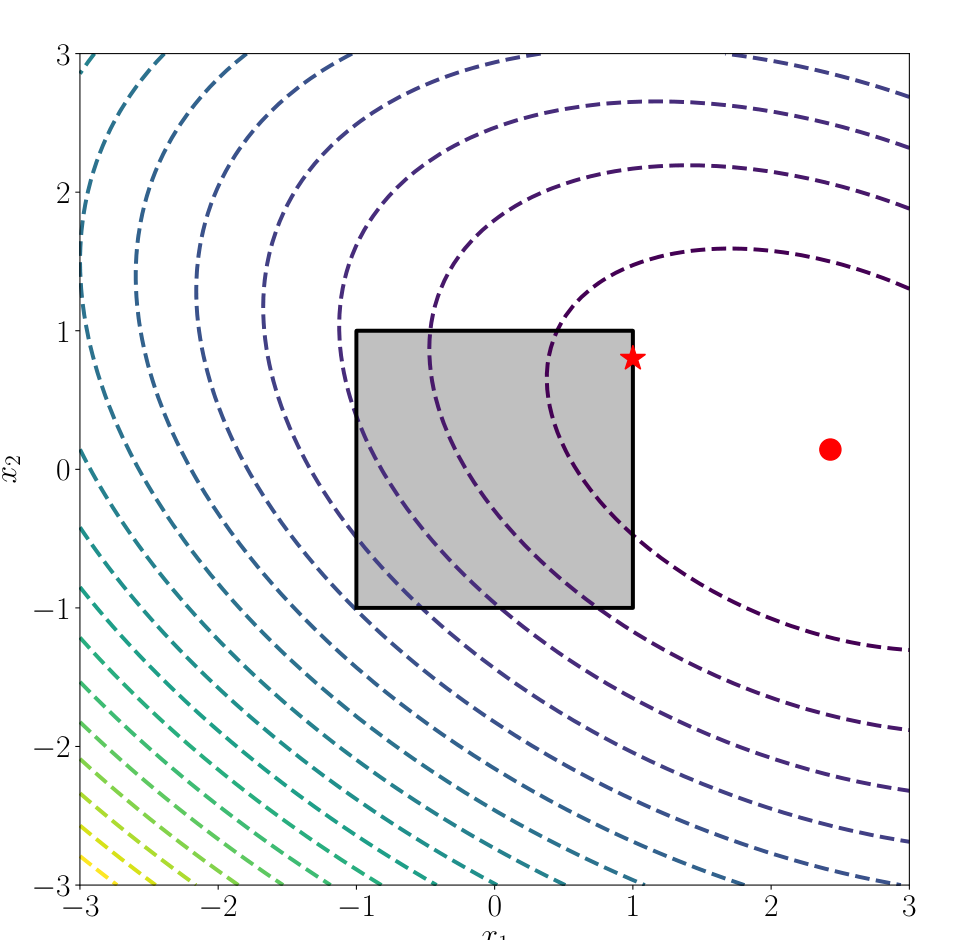
\includegraphics[width=320pt,keepaspectratio]{docs/images/Figure7.4.png}
\caption*{\refstepcounter{figcounter}\label{fig:7-4}图~\thefigcounter 带约束优化示意图。}
\end{figure}


值得指出的是，在一般情况下，函数 $ f $ 和 $ g_i $ 可能是非凸的，我们将在下一节中讨论凸的情形。

将带约束问题 (7.17) 转化为无约束问题的一种显而易见但不太实用的方法是使用 \emph{示性函数（indicator function）} ：

\begin{equation}
J(\boldsymbol{x}) = f(\boldsymbol{x}) + \sum_{i=1}^m \mathbf{1}(g_i(\boldsymbol{x}))
\tag{7.18}\label{eq:7-18}
\end{equation}

其中 $ \mathbf{1}(z) $ 是一个无穷阶跃函数：

\begin{equation}
\mathbf{1}(z) = \begin{cases} 0 & \textcn{若 } z \leqslant 0 \\ \infty & \textcn{其他} \end{cases} \textcn{。}
\tag{7.19}\label{eq:7-19}
\end{equation}

当约束不满足时，该函数会施加无穷大的惩罚，因此能够提供与原问题相同的解。然而，这个无穷阶跃函数在优化上同样极其困难。我们可以通过引入 \emph{拉格朗日乘子（Lagrange multiplier）} 来克服这一困难。拉格朗日乘子的核心思想是用线性函数来替代该阶跃函数。

通过分别为每个不等式约束引入拉格朗日乘子 $ \lambda_i \geqslant 0 $（Boyd and Vandenberghe, 2004, chapter 4），我们将问题 (7.17) 与 \emph{拉格朗日函数（Lagrangian）} 联系起来，使得：

\begin{equation}
\mathfrak{L}(\boldsymbol{x}, \boldsymbol{\lambda}) = f(\boldsymbol{x}) + \sum_{i=1}^m \lambda_i g_i(\boldsymbol{x})
\tag{7.20a}\label{eq:7-20a}
\end{equation}

\begin{equation}
= f(\boldsymbol{x}) + \boldsymbol{\lambda}^\top \boldsymbol{g}(\boldsymbol{x})
\tag{7.20b}\label{eq:7-20b}
\end{equation}

在最后一行中，我们将所有约束 $ g_i(\boldsymbol{x}) $ 拼接成向量 $ \boldsymbol{g}(\boldsymbol{x}) $，并将所有拉格朗日乘子拼接成向量 $ \boldsymbol{\lambda} \in \mathbb{R}^m $。

现在我们引入拉格朗日对偶的思想。一般而言，优化中的对偶性是指将一组变量 $ \boldsymbol{x} $（称为 \emph{原变量（primal variables）} ）的优化问题，转化为另一组不同变量 $ \boldsymbol{\lambda} $（称为 \emph{对偶变量（dual variables）} ）的优化问题。我们介绍两种不同的对偶途径：在本节中，我们讨论 \emph{拉格朗日对偶（Lagrangian duality）} ；在第 7.3.3 节中，我们将讨论 \emph{勒让德-芬歇尔对偶（Legendre–Fenchel duality）} 。

\textbf{定义 7.1}。式~\eqref{eq:7-17} 中的问题：

\begin{equation}
\begin{aligned}
\min_{\boldsymbol{x}} & \quad f(\boldsymbol{x}) \\
\text{subject to} & \quad g_i(\boldsymbol{x}) \leqslant 0 \quad \textcn{对所有 } i = 1, \ldots, m
\end{aligned}
\tag{7.21}\label{eq:7-21}
\end{equation}

被称为 \emph{原问题（primal problem）} ，对应于原变量 $ \boldsymbol{x} $。 其相应的 \emph{拉格朗日对偶问题（Lagrangian dual problem）} 由下式给出：

\begin{equation}
\begin{aligned}
\max_{\boldsymbol{\lambda} \in \mathbb{R}^m} & \quad \mathfrak{D}(\boldsymbol{\lambda}) \\
\text{subject to} & \quad \boldsymbol{\lambda} \geqslant \boldsymbol{0} ,
\end{aligned}
\tag{7.22}\label{eq:7-22}
\end{equation}

其中 $ \boldsymbol{\lambda} $ 是对偶变量，且 $ \mathfrak{D}(\boldsymbol{\lambda}) = \min_{\boldsymbol{x} \in \mathbb{R}^d} \mathfrak{L}(\boldsymbol{x}, \boldsymbol{\lambda}) $。

\emph{备注} 。在定义 7.1 的讨论中，我们使用了两个同样具有独立重要意义的概念（Boyd and Vandenberghe, 2004）。

首先是 \emph{极小极大不等式（minimax inequality）} ，它指出对于任意具有两个参数的函数 $ \phi(\boldsymbol{x}, \boldsymbol{y}) $，先极小后极大（maximin）小于等于先极大后极小（minimax），即：

\begin{equation}
\max_{\boldsymbol{y}} \min_{\boldsymbol{x}} \phi(\boldsymbol{x}, \boldsymbol{y}) \leqslant \min_{\boldsymbol{x}} \max_{\boldsymbol{y}} \phi(\boldsymbol{x}, \boldsymbol{y}) \textcn{。}
\tag{7.23}\label{eq:7-23}
\end{equation}

该不等式可以通过考虑以下不等式来证明：

\begin{equation}
\textcn{对所有 } \boldsymbol{x}, \boldsymbol{y} , \quad \min_{\boldsymbol{x}} \phi(\boldsymbol{x}, \boldsymbol{y}) \leqslant \max_{\boldsymbol{y}} \phi(\boldsymbol{x}, \boldsymbol{y}) \textcn{。}
\tag{7.24}\label{eq:7-24}
\end{equation}

注意到对式~\eqref{eq:7-24} 的左侧关于 $ \boldsymbol{y} $ 取极大值仍然保持不等式成立，因为该不等式对所有 $ \boldsymbol{y} $ 均成立。类似地，我们可以对式~\eqref{eq:7-24} 的右侧关于 $ \boldsymbol{x} $ 取极小值，从而得到式~\eqref{eq:7-23}。

第二个概念是 \emph{弱对偶性（weak duality）} ，它利用式~\eqref{eq:7-23} 证明了原问题的值始终大于或等于对偶问题的值。这在式~\eqref{eq:7-27} 中有更详细的描述。♦

回想一下，式~\eqref{eq:7-18} 中的 $ J(\boldsymbol{x}) $ 与式~\eqref{eq:7-20b} 中的拉格朗日函数之间的区别在于，我们将示性函数松弛为了线性函数。因此，当 $ \boldsymbol{\lambda} \geqslant \boldsymbol{0} $ 时，拉格朗日函数 $ \mathfrak{L}(\boldsymbol{x}, \boldsymbol{\lambda}) $ 是 $ J(\boldsymbol{x}) $ 的下界。因此，$ \mathfrak{L}(\boldsymbol{x}, \boldsymbol{\lambda}) $ 关于 $ \boldsymbol{\lambda} $ 的极大值为：

\begin{equation}
J(\boldsymbol{x}) = \max_{\boldsymbol{\lambda} \geqslant \boldsymbol{0}} \mathfrak{L}(\boldsymbol{x}, \boldsymbol{\lambda}) \textcn{。}
\tag{7.25}\label{eq:7-25}
\end{equation}

回想一下，原始问题是极小化 $ J(\boldsymbol{x}) $：

\begin{equation}
\min_{\boldsymbol{x} \in \mathbb{R}^d} \max_{\boldsymbol{\lambda} \geqslant \boldsymbol{0}} \mathfrak{L}(\boldsymbol{x}, \boldsymbol{\lambda}) \textcn{。}
\tag{7.26}\label{eq:7-26}
\end{equation}

根据极小极大不等式~\eqref{eq:7-23}，交换极小与极大的顺序会产生一个较小的值，即：

\begin{equation}
\begin{adjustbox}{max width=\linewidth}
\min_{\boldsymbol{x} \in \mathbb{R}^d} \max_{\boldsymbol{\lambda} \geqslant \boldsymbol{0}} \mathfrak{L}(\boldsymbol{x}, \boldsymbol{\lambda}) \geqslant \max_{\boldsymbol{\lambda} \geqslant \boldsymbol{0}} \min_{\boldsymbol{x} \in \mathbb{R}^d} \mathfrak{L}(\boldsymbol{x}, \boldsymbol{\lambda}) \textcn{。}
\end{adjustbox}
\tag{7.27}\label{eq:7-27}
\end{equation}

这也称为 \emph{弱对偶性（weak duality）} 。注意到右侧的内部部分正是 \emph{对偶目标函数（dual objective function）} $ \mathfrak{D}(\boldsymbol{\lambda}) $，定义由此自然得出。

与带有约束的原始优化问题相比，对于给定的 $ \boldsymbol{\lambda} $ 值，$ \min_{\boldsymbol{x} \in \mathbb{R}^d} \mathfrak{L}(\boldsymbol{x}, \boldsymbol{\lambda}) $ 是一个无约束优化问题。如果求解 $ \min_{\boldsymbol{x} \in \mathbb{R}^d} \mathfrak{L}(\boldsymbol{x}, \boldsymbol{\lambda}) $ 很简单，那么整个问题就容易求解。原因在于外层问题（关于 $ \boldsymbol{\lambda} $ 的极大化）是一组仿射函数的逐点极大值，因此即便 $ f(\cdot) $ 和 $ g_i(\cdot) $ 可能非凸，它也是一个凹函数。凹函数的极大值可以被高效地计算。

假定 $ f(\cdot) $ 和 $ g_i(\cdot) $ 是可微的，我们通过对拉格朗日函数关于 $ \boldsymbol{x} $ 求微分，令微分（导数）为零，并解出最优值，从而求得拉格朗日对偶问题。我们将在第 7.3.1 节和第 7.3.2 节中讨论两个具体示例，其中 $ f(\cdot) $ 和 $ g_i(\cdot) $ 均是凸的。

\emph{备注} （等式约束）。考虑式~\eqref{eq:7-17} 带有额外等式约束的情形：

\begin{equation}
\begin{adjustbox}{max width=\linewidth}
\begin{aligned}
\min_{\boldsymbol{x}} & \quad f(\boldsymbol{x}) \\
\text{subject to} & \quad g_i(\boldsymbol{x}) \leqslant 0 \quad \textcn{对所有 } i = 1, \ldots, m \\
& \quad h_j(\boldsymbol{x}) = 0 \quad \textcn{对所有 } j = 1, \ldots, n \textcn{。}
\end{aligned}
\end{adjustbox}
\tag{7.28}\label{eq:7-28}
\end{equation}

我们可以通过将等式约束替换为两个不等式约束来对其进行建模。也就是说，对于每个等式约束 $ h_j(\boldsymbol{x}) = 0 $，我们将其等价替换为两个约束 $ h_j(\boldsymbol{x}) \leqslant 0 $ 和 $ h_j(\boldsymbol{x}) \geqslant 0 $。事实证明，由此得到的拉格朗日乘子是不受约束的。

因此，我们对式~\eqref{eq:7-28} 中对应于不等式约束的拉格朗日乘子施加非负约束，而对应于等式约束的拉格朗日乘子则不受约束。♦

\section*{7.3 凸优化}
\addcontentsline{toc}{section}{7.3 凸优化}
\label{sec:7.3}

我们将注意力集中在一类特别有用的优化问题上，在这些问题中我们可以保证全局最优性。当 $ f(\cdot) $ 是凸函数，且涉及 $ g(\cdot) $ 和 $ h(\cdot) $ 的约束是凸集时，这被称为 \emph{凸优化问题（convex optimization problem）} 。在此设定下，我们拥有 \emph{强对偶性（strong duality）} ：对偶问题的最优解与原问题的最优解相同。在机器学习文献中，凸函数与凸集之间的区别往往并未严格区分，但通常可以从上下文中推断出其隐含含义。

\textbf{定义 7.2}（凸集）。若对于任意 $ \boldsymbol{x}, \boldsymbol{y} \in C $ 以及任意满足 $ 0 \leqslant \theta \leqslant 1 $ 的标量 $ \theta $，均有：

\begin{equation}
\theta \boldsymbol{x} + (1 - \theta)\boldsymbol{y} \in C
\tag{7.29}\label{eq:7-29}
\end{equation}

则集合 $ C $ 是一个 \emph{凸集（convex set）} 。


\begin{figure}[H]
\centering
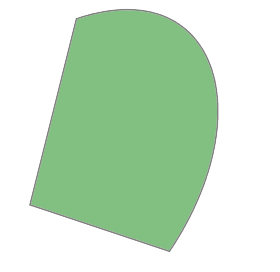
\includegraphics[width=320pt,keepaspectratio]{docs/images/Figure7.5.png}
\caption*{\refstepcounter{figcounter}\label{fig:7-5}图~\thefigcounter 凸集示例。}
\end{figure}


凸集是指连接集合中任意两点的线段完全位于集合内部的集合。图~\ref{fig:7-5} 和图~\ref{fig:7-6} 分别说明了凸集与非凸集。


\begin{figure}[H]
\centering

\includegraphics[width=0.92\textwidth,keepaspectratio]{docs/images/Figure7.6.png}
\caption*{\refstepcounter{figcounter}\label{fig:7-6}图~\thefigcounter 非凸集示例。}
\end{figure}


凸函数是指连接函数图像上任意两点的线段位于函数图像上方的函数。图~\ref{fig:7-2} 展示了一个非凸函数，图~\ref{fig:7-3} 展示了一个凸函数。另一个凸函数如图~\ref{fig:7-7} 所示。

\textbf{定义 7.3}（凸函数）。设函数 $ f : \mathbb{R}^D \to \mathbb{R} $ 的定义域为凸集。若对于 $ f $ 定义域内的所有 $ \boldsymbol{x}, \boldsymbol{y} $ 以及任意满足 $ 0 \leqslant \theta \leqslant 1 $ 的标量 $ \theta $，均有：

\begin{equation}
f(\theta \boldsymbol{x} + (1 - \theta)\boldsymbol{y}) \leqslant \theta f(\boldsymbol{x}) + (1 - \theta)f(\boldsymbol{y})
\tag{7.30}\label{eq:7-30}
\end{equation}

则函数 $ f $ 是一个 \emph{凸函数（convex function）} 。

\emph{备注} 。 \emph{凹函数（concave function）} 是凸函数的相反数。♦

式~\eqref{eq:7-28} 中涉及 $ g(\cdot) $ 和 $ h(\cdot) $ 的约束将函数截断在某个标量值处，从而形成集合。凸函数与凸集之间的另一种联系是考虑通过“填满”一个凸函数所得到的集合。凸函数是一个碗状物体，我们可以想象向其中注水将其填满。所得到的这个填满的集合称为凸函数的 \emph{上图（epigraph）} ，它是一个凸集。

若函数 $ f : \mathbb{R}^n \to \mathbb{R} $ 是可微的，我们可以利用其梯度 $ \nabla_{\boldsymbol{x}} f(\boldsymbol{x}) $（第 5.2 节）来刻画凸性。函数 $ f(\boldsymbol{x}) $ 是凸函数当且仅当对于任意两点 $ \boldsymbol{x}, \boldsymbol{y} $，均满足：

\begin{equation}
f(\boldsymbol{y}) \geqslant f(\boldsymbol{x}) + \nabla_{\boldsymbol{x}} f(\boldsymbol{x})^\top (\boldsymbol{y} - \boldsymbol{x})
\tag{7.31}\label{eq:7-31}
\end{equation}

如果我们进一步知道函数 $ f(\boldsymbol{x}) $ 是二阶可微的，即对于 $ \boldsymbol{x} $ 定义域内的所有取值，Hessian 矩阵（式~\eqref{eq:5-147}）均存在，那么函数 $ f(\boldsymbol{x}) $ 为凸函数当且仅当 $ \nabla_{\boldsymbol{x}}^2 f(\boldsymbol{x}) $ 是半正定的（Boyd and Vandenberghe, 2004）。


\begin{figure}[H]
\centering
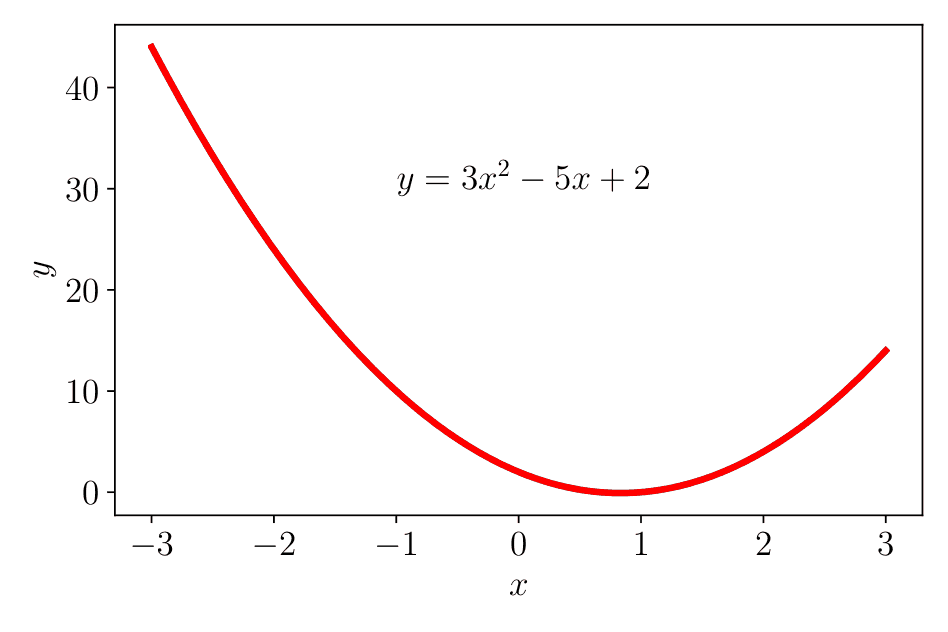
\includegraphics[width=0.92\textwidth,keepaspectratio]{docs/images/Figure7.7.png}
\caption*{\refstepcounter{figcounter}\label{fig:7-7}图~\thefigcounter 凸函数示例。}
\end{figure}


\begin{notebox}
\textbf{例 7.3}
\end{notebox}

\begin{notebox}
负熵函数 $ f(x) = x \log_2 x $ 在 $ x > 0 $ 时是凸函数。该函数的几何图像如图~\ref{fig:7-8} 所示，我们可以看出它是凸函数。为了说明前面的凸性定义，让我们用两点 $ x = 2 $ 和 $ x = 4 $ 来进行验算。请注意，要证明 $ f(x) $ 的凸性，我们需要检验定义域内所有的点 $ x \in \mathbb{R} $。
\end{notebox}

\begin{notebox}
回顾定义 7.3。考虑两点中点处的位置（即 $ \theta = 0.5 $），则左侧为 $ f(0.5 \cdot 2 + 0.5 \cdot 4) = 3 \log_2 3 \approx 4.75 $。右侧为 $ 0.5(2 \log_2 2) + 0.5(4 \log_2 4) = 1 + 4 = 5 $。因此满足定义。
\end{notebox}

\begin{notebox}
由于 $ f(x) $ 是可微的，我们也可以使用式~\eqref{eq:7-31}。计算 $ f(x) $ 的导数，我们得到：

\begin{equation}
\nabla_x (x \log_2 x) = 1 \cdot \log_2 x + x \cdot \frac{1}{x \log_e 2} = \log_2 x + \frac{1}{\log_e 2}
\tag{7.32}\label{eq:7-32}
\end{equation}

使用相同的两个测试点 $ x = 2 $ 和 $ x = 4 $，式~\eqref{eq:7-31} 的左侧为 $ f(4) = 8 $。右侧为：

\begin{equation}
f(x) + \nabla_x f(x)^\top (y - x) = f(2) + \nabla f(2) \cdot (4 - 2)
\tag{7.33a}\label{eq:7-33a}
\end{equation}

\begin{equation}
= 2 + \left( 1 + \frac{1}{\log_e 2} \right) \cdot 2 \approx 6.9
\tag{7.33b}\label{eq:7-33b}
\end{equation}
\end{notebox}


\begin{figure}[H]
\centering
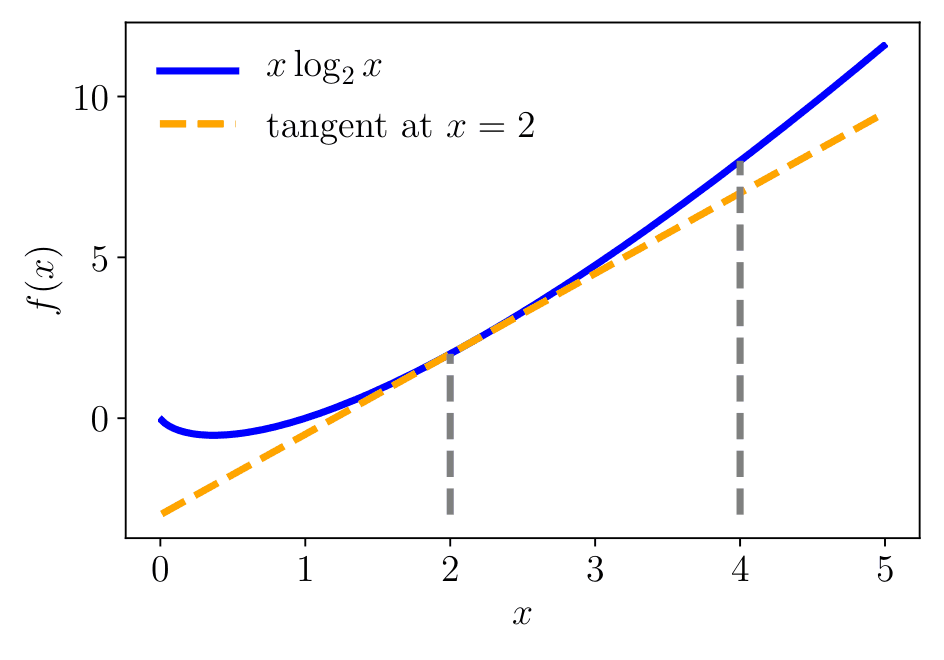
\includegraphics[width=0.92\textwidth,keepaspectratio]{docs/images/Figure7.8.png}
\caption*{\refstepcounter{figcounter}\label{fig:7-8}图~\thefigcounter 负熵函数（凸函数）及其在 x = 2 处的切线。}
\end{figure}


我们可以通过回顾定义，从第一性原理检验一个函数或集合是否为凸的。在实践中，我们通常依赖于保持凸性的运算来检验特定函数或集合的凸性。尽管细节大相径庭，但这再次体现了我们在第 2 章针对向量空间介绍的闭包思想。

\begin{notebox}
\textbf{例 7.4}
\end{notebox}

\begin{notebox}
凸函数的非负加权和是凸的。注意到若 $ f $ 是凸函数，且 $ \alpha \geqslant 0 $ 是非负标量，则函数 $ \alpha f $ 是凸的。我们可以通过在定义 7.3 的不等式两边乘以 $ \alpha $ 看出这一点，并回想乘以非负数不会改变不等号方向。
\end{notebox}

\begin{notebox}
若 $ f_1 $ 和 $ f_2 $ 是凸函数，则根据定义有：

\begin{equation}
f_1(\theta \boldsymbol{x} + (1 - \theta)\boldsymbol{y}) \leqslant \theta f_1(\boldsymbol{x}) + (1 - \theta)f_1(\boldsymbol{y})
\tag{7.34}\label{eq:7-34}
\end{equation}

\begin{equation}
f_2(\theta \boldsymbol{x} + (1 - \theta)\boldsymbol{y}) \leqslant \theta f_2(\boldsymbol{x}) + (1 - \theta)f_2(\boldsymbol{y})
\tag{7.35}\label{eq:7-35}
\end{equation}

两边相加得到：

\begin{equation}
\begin{adjustbox}{max width=\linewidth}
f_1(\theta \boldsymbol{x} + (1 - \theta)\boldsymbol{y}) + f_2(\theta \boldsymbol{x} + (1 - \theta)\boldsymbol{y}) \leqslant \theta f_1(\boldsymbol{x}) + (1 - \theta)f_1(\boldsymbol{y}) + \theta f_2(\boldsymbol{x}) + (1 - \theta)f_2(\boldsymbol{y})
\end{adjustbox}
\tag{7.36}\label{eq:7-36}
\end{equation}

其中右侧可以重新整理为：

\begin{equation}
\theta (f_1(\boldsymbol{x}) + f_2(\boldsymbol{x})) + (1 - \theta)(f_1(\boldsymbol{y}) + f_2(\boldsymbol{y}))
\tag{7.37}\label{eq:7-37}
\end{equation}

从而完成了两凸函数之和为凸函数的证明。
\end{notebox}

\begin{notebox}
结合上述两个事实，我们看到对于 $ \alpha, \beta \geqslant 0 $，$ \alpha f_1(\boldsymbol{x}) + \beta f_2(\boldsymbol{x}) $ 是凸函数。使用类似的论证，该闭包性质可以推广到两个以上凸函数的非负加权和。
\end{notebox}

\emph{备注} 。式~\eqref{eq:7-30} 中的不等式有时被称为 \emph{琴生不等式（Jensen's inequality）} 。事实上，一整类关于取凸函数非负加权和的不等式都被称为琴生不等式。♦

总而言之，一个带约束优化问题若具有如下形式，则称为 \emph{凸优化问题（convex optimization problem）} ：

\begin{equation}
\begin{adjustbox}{max width=\linewidth}
\begin{aligned}
\min_{\boldsymbol{x}} \quad & f(\boldsymbol{x}) \\
\text{subject to} \quad & g_i(\boldsymbol{x}) \leqslant 0 \quad \textcn{对所有 } i = 1, \ldots, m \\
& h_j(\boldsymbol{x}) = 0 \quad \textcn{对所有 } j = 1, \ldots, n
\end{aligned}
\end{adjustbox}
\tag{7.38}\label{eq:7-38}
\end{equation}

其中所有函数 $ f(\boldsymbol{x}) $ 和 $ g_i(\boldsymbol{x}) $ 均为凸函数，且所有 $ h_j(\boldsymbol{x}) = 0 $ 均为凸集。在下文中，我们将描述两类应用广泛且已被充分理解的凸优化问题。

\section*{7.3.1 线性规划}
\addcontentsline{toc}{subsection}{7.3.1 线性规划}

考虑上述所有函数均为线性的特殊情形，即：

\begin{equation}
\begin{aligned}
\min_{\boldsymbol{x} \in \mathbb{R}^d} \quad & \boldsymbol{c}^\top \boldsymbol{x} \\
\text{subject to} \quad & \boldsymbol{A} \boldsymbol{x} \leqslant \boldsymbol{b}
\end{aligned}
\tag{7.39}\label{eq:7-39}
\end{equation}

其中 $ \boldsymbol{A} \in \mathbb{R}^{m \times d} $ 且 $ \boldsymbol{b} \in \mathbb{R}^m $。这被称为 \emph{线性规划（linear program）} （ \emph{边注} ：线性规划是工业界应用最广泛的方法之一。）。它具有 $ d $ 个变量和 $ m $ 个线性约束。拉格朗日函数由下式给出：

\begin{equation}
L(\boldsymbol{x}, \boldsymbol{\lambda}) = \boldsymbol{c}^\top \boldsymbol{x} + \boldsymbol{\lambda}^\top (\boldsymbol{A} \boldsymbol{x} - \boldsymbol{b})
\tag{7.40}\label{eq:7-40}
\end{equation}

其中 $ \boldsymbol{\lambda} \in \mathbb{R}^m $ 是非负拉格朗日乘子构成的向量。重排对应于 $ \boldsymbol{x} $ 的各项得到：

\begin{equation}
L(\boldsymbol{x}, \boldsymbol{\lambda}) = (\boldsymbol{c} + \boldsymbol{A}^\top \boldsymbol{\lambda})^\top \boldsymbol{x} - \boldsymbol{\lambda}^\top \boldsymbol{b}
\tag{7.41}\label{eq:7-41}
\end{equation}

对 $ L(\boldsymbol{x}, \boldsymbol{\lambda}) $ 关于 $ \boldsymbol{x} $ 求导并令其为零，得到：

\begin{equation}
\boldsymbol{c} + \boldsymbol{A}^\top \boldsymbol{\lambda} = \boldsymbol{0}
\tag{7.42}\label{eq:7-42}
\end{equation}

因此，对偶拉格朗日函数为 $ D(\boldsymbol{\lambda}) = -\boldsymbol{\lambda}^\top \boldsymbol{b} $。回想一下，我们希望最大化 $ D(\boldsymbol{\lambda}) $。除了由 $ L(\boldsymbol{x}, \boldsymbol{\lambda}) $ 的导数为零所产生的约束外，我们还有 $ \boldsymbol{\lambda} \geqslant \boldsymbol{0} $ 这一事实，从而得到如下对偶优化问题（ \emph{边注} ：通常的约定是最小化原问题并最大化对偶问题。）：

\begin{equation}
\begin{adjustbox}{max width=\linewidth}
\begin{aligned}
\max_{\boldsymbol{\lambda} \in \mathbb{R}^m} \quad & -\boldsymbol{b}^\top \boldsymbol{\lambda} \\
\text{subject to} \quad & \boldsymbol{c} + \boldsymbol{A}^\top \boldsymbol{\lambda} = \boldsymbol{0} \\
& \boldsymbol{\lambda} \geqslant \boldsymbol{0}
\end{aligned}
\end{adjustbox}
\tag{7.43}\label{eq:7-43}
\end{equation}

这也是一个线性规划，但具有 $ m $ 个变量。根据 $ m $ 与 $ d $ 孰大孰小，我们可以灵活选择求解原问题 (7.39) 或对偶问题 (7.43)。回想一下，$ d $ 是原线性规划中的变量数，而 $ m $ 是约束数。

\begin{notebox}
\textbf{例 7.5（线性规划）}
\end{notebox}

\begin{notebox}
考虑包含两个变量的线性规划：

\begin{equation}
\begin{adjustbox}{max width=\linewidth}
\begin{aligned}
\min_{\boldsymbol{x} \in \mathbb{R}^2} \quad & -\begin{bmatrix} 5 \\ 3 \end{bmatrix}^\top \begin{bmatrix} x_1 \\ x_2 \end{bmatrix} \\
\text{subject to} \quad & \begin{bmatrix} 2 & 2 \\ 2 & -4 \\ -2 & 1 \\ 0 & -1 \\ 0 & 1 \end{bmatrix} \begin{bmatrix} x_1 \\ x_2 \end{bmatrix} \leqslant \begin{bmatrix} 33 \\ 8 \\ 5 \\ -1 \\ 8 \end{bmatrix}
\end{aligned}
\end{adjustbox}
\tag{7.44}\label{eq:7-44}
\end{equation}

该规划也在图~\ref{fig:7-9} 中进行了展示。目标函数是线性的，因此等高线呈线性直线。标准形式的约束集被转化并标注在图例中。最优值必须位于阴影（可行）区域内，并由星号指示。
\end{notebox}


\begin{figure}[H]
\centering
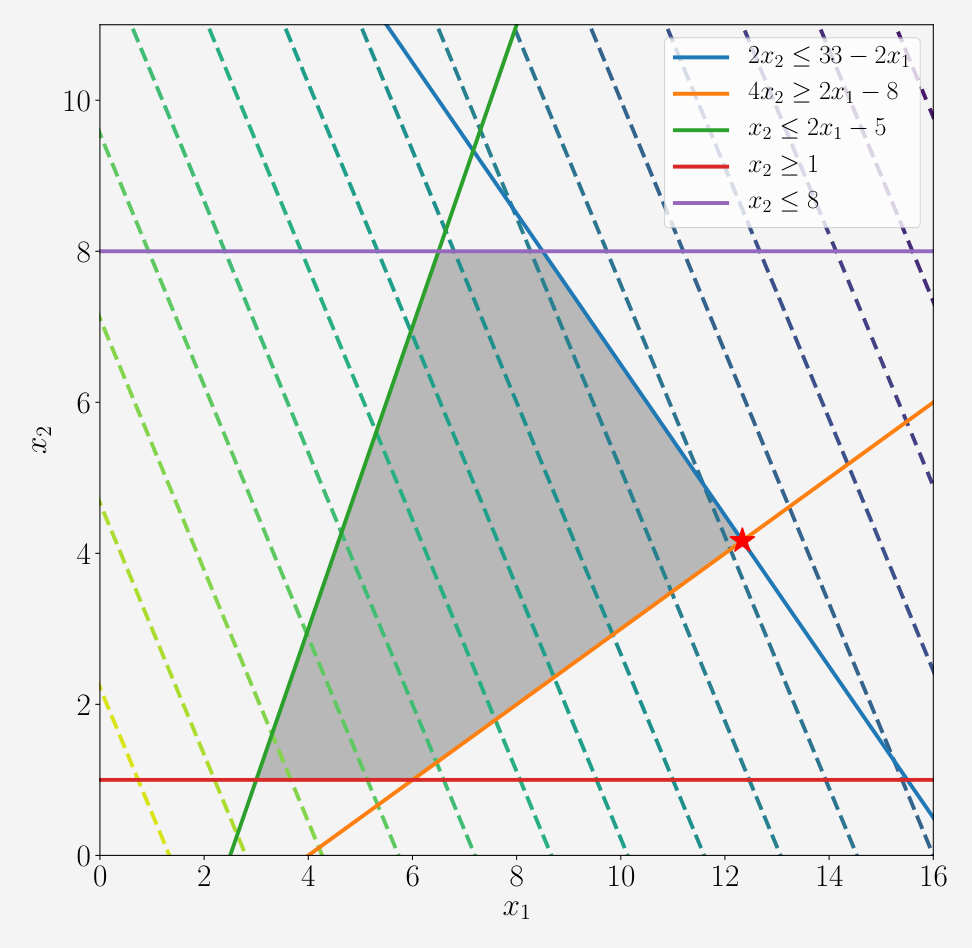
\includegraphics[width=320pt,keepaspectratio]{docs/images/Figure7.9.png}
\caption*{\refstepcounter{figcounter}\label{fig:7-9}图~\thefigcounter 线性规划示意图。无约束问题（由等高线指示）在右侧具有极小值。满足约束条件的最优值由星号指示。}
\end{figure}


\section*{7.3.2 二次规划}
\addcontentsline{toc}{subsection}{7.3.2 二次规划}

考虑目标函数为凸二次函数、约束为仿射约束的情形，即：

\begin{equation}
\begin{adjustbox}{max width=\linewidth}
\begin{aligned}
\min_{\boldsymbol{x} \in \mathbb{R}^d} \quad & \frac{1}{2}\boldsymbol{x}^\top \boldsymbol{Q} \boldsymbol{x} + \boldsymbol{c}^\top \boldsymbol{x} \\
\text{subject to} \quad & \boldsymbol{A} \boldsymbol{x} \leqslant \boldsymbol{b}
\end{aligned}
\end{adjustbox}
\tag{7.45}\label{eq:7-45}
\end{equation}

其中 $ \boldsymbol{A} \in \mathbb{R}^{m \times d} $，$ \boldsymbol{b} \in \mathbb{R}^m $，且 $ \boldsymbol{c} \in \mathbb{R}^d $。对称方阵 $ \boldsymbol{Q} \in \mathbb{R}^{d \times d} $ 是正定的，因此目标函数是凸函数。这被称为 \emph{二次规划（quadratic program）} 。容易看出，它具有 $ d $ 个变量和 $ m $ 个线性约束。

\begin{notebox}
\textbf{例 7.6（二次规划）}
\end{notebox}

\begin{notebox}
考虑包含两个变量的二次规划：

\begin{equation}
\begin{adjustbox}{max width=\linewidth}
\min_{\boldsymbol{x} \in \mathbb{R}^2} \quad \frac{1}{2} \begin{bmatrix} x_1 \\ x_2 \end{bmatrix}^\top \begin{bmatrix} 2 & 1 \\ 1 & 4 \end{bmatrix} \begin{bmatrix} x_1 \\ x_2 \end{bmatrix} + \begin{bmatrix} 5 \\ 3 \end{bmatrix}^\top \begin{bmatrix} x_1 \\ x_2 \end{bmatrix}
\end{adjustbox}
\tag{7.46}\label{eq:7-46}
\end{equation}

\begin{equation}
\text{subject to} \quad \begin{bmatrix} 1 & 0 \\ -1 & 0 \\ 0 & 1 \\ 0 & -1 \end{bmatrix} \begin{bmatrix} x_1 \\ x_2 \end{bmatrix} \leqslant \begin{bmatrix} 1 \\ 1 \\ 1 \\ 1 \end{bmatrix}
\tag{7.47}\label{eq:7-47}
\end{equation}

该规划也在图~\ref{fig:7-4} 中进行了展示。目标函数是带有半正定矩阵 $ \boldsymbol{Q} $ 的二次函数，产生椭圆形的等高线。最优值必须位于阴影（可行）区域内，并由星号指示。
\end{notebox}

拉格朗日函数由下式给出：

\begin{equation}
L(\boldsymbol{x}, \boldsymbol{\lambda}) = \frac{1}{2}\boldsymbol{x}^\top \boldsymbol{Q} \boldsymbol{x} + \boldsymbol{c}^\top \boldsymbol{x} + \boldsymbol{\lambda}^\top (\boldsymbol{A} \boldsymbol{x} - \boldsymbol{b})
\tag{7.48a}\label{eq:7-48a}
\end{equation}

\begin{equation}
= \frac{1}{2}\boldsymbol{x}^\top \boldsymbol{Q} \boldsymbol{x} + (\boldsymbol{c} + \boldsymbol{A}^\top \boldsymbol{\lambda})^\top \boldsymbol{x} - \boldsymbol{\lambda}^\top \boldsymbol{b}
\tag{7.48b}\label{eq:7-48b}
\end{equation}

这里我们再次重排了各项。对 $ L(\boldsymbol{x}, \boldsymbol{\lambda}) $ 关于 $ \boldsymbol{x} $ 求导并令其为零，得到：

\begin{equation}
\boldsymbol{Q} \boldsymbol{x} + (\boldsymbol{c} + \boldsymbol{A}^\top \boldsymbol{\lambda}) = \boldsymbol{0}
\tag{7.49}\label{eq:7-49}
\end{equation}

假设 $ \boldsymbol{Q} $ 是可逆的，我们得到：

\begin{equation}
\boldsymbol{x} = -\boldsymbol{Q}^{-1}(\boldsymbol{c} + \boldsymbol{A}^\top \boldsymbol{\lambda})
\tag{7.50}\label{eq:7-50}
\end{equation}

将式~\eqref{eq:7-50} 代入原拉格朗日函数 $ L(\boldsymbol{x}, \boldsymbol{\lambda}) $，得到对偶拉格朗日函数：

\begin{equation}
\begin{adjustbox}{max width=\linewidth}
D(\boldsymbol{\lambda}) = -\frac{1}{2}(\boldsymbol{c} + \boldsymbol{A}^\top \boldsymbol{\lambda})^\top \boldsymbol{Q}^{-1}(\boldsymbol{c} + \boldsymbol{A}^\top \boldsymbol{\lambda}) - \boldsymbol{\lambda}^\top \boldsymbol{b}
\end{adjustbox}
\tag{7.51}\label{eq:7-51}
\end{equation}

因此，对偶优化问题由下式给出：

\begin{equation}
\begin{adjustbox}{max width=\linewidth}
\begin{aligned}
\max_{\boldsymbol{\lambda} \in \mathbb{R}^m} \quad & -\frac{1}{2}(\boldsymbol{c} + \boldsymbol{A}^\top \boldsymbol{\lambda})^\top \boldsymbol{Q}^{-1}(\boldsymbol{c} + \boldsymbol{A}^\top \boldsymbol{\lambda}) - \boldsymbol{\lambda}^\top \boldsymbol{b} \\
\text{subject to} \quad & \boldsymbol{\lambda} \geqslant \boldsymbol{0}
\end{aligned}
\end{adjustbox}
\tag{7.52}\label{eq:7-52}
\end{equation}

我们将在第 12 章中看到二次规划在机器学习中的应用。

\section*{7.3.3 勒让德-芬彻尔变换与凸共轭}
\addcontentsline{toc}{subsection}{7.3.3 勒让德-芬彻尔变换与凸共轭}

让我们在不考虑约束的情况下，重新审视第 7.2 节中的对偶思想。关于凸集的一个有用事实是，它可以等价地由其支撑超平面来描述。如果一个超平面与凸集相交，且凸集完全包含在该超平面的某一侧，则称该超平面为凸集的 \emph{支撑超平面（supporting hyperplane）} 。回想一下，我们可以填满一个凸函数以获得其上图，而上图是一个凸集。因此，我们也可以借助支撑超平面来描述凸函数。此外，观察到支撑超平面恰好与凸函数相切，事实上就是该点处函数的切线。并且回想一下，函数 $ f(x) $ 在给定点 $ x_0 $ 处的切线斜率是该函数在该点处的导数求值 $ \left.\frac{\mathrm{d}f(x)}{\mathrm{d}x}\right|_{x=x_0} $。

总而言之，因为凸集可以等价地由其支撑超平面描述，所以凸函数可以等价地由关于其梯度的函数来描述。 \emph{勒让德变换（Legendre transform）} 将这一概念形式化（ \emph{边注} ：物理系学生通常通过经典力学中连接拉格朗日量与哈密顿量的工具来初次接触勒让德变换。）。

我们首先给出最一般的定义（遗憾的是它的形式可能有些反直觉），然后通过特例将该定义与上一段所描述的直觉联系起来。 \emph{勒让德-芬彻尔变换（Legendre–Fenchel transform）} 是从凸可微函数 $ f(\boldsymbol{x}) $ 到依赖于切线斜率（梯度）$ \boldsymbol{s}(\boldsymbol{x}) = \nabla_{\boldsymbol{x}} f(\boldsymbol{x}) $ 的函数的变换（在类似于傅里叶变换的意义下）。值得强调的是，这是函数 $ f(\cdot) $ 本身的变换，而不是变量 $ \boldsymbol{x} $ 或在 $ \boldsymbol{x} $ 处求值的函数值的变换。勒让德-芬彻尔变换也被称为 \emph{凸共轭（convex conjugate）} （原因我们很快就会看到），并且与对偶性密切相关（Hiriart-Urruty and Lemaréchal, 2001，第 5 章）。

\textbf{定义 7.4}（凸共轭）。函数 $ f : \mathbb{R}^D \to \mathbb{R} $ 的 \emph{凸共轭（convex conjugate）} 是由下式定义的函数 $ f^* $：

\begin{equation}
f^*(\boldsymbol{s}) = \sup_{\boldsymbol{x} \in \mathbb{R}^D} \left( \langle \boldsymbol{s}, \boldsymbol{x} \rangle - f(\boldsymbol{x}) \right)
\tag{7.53}\label{eq:7-53}
\end{equation}

注意到上述凸共轭定义既不需要函数 $ f $ 是凸的，也不需要它是可微的。在定义 7.4 中，我们使用了广义内积（第 3.2 节），但在本节的其余部分中，我们将考虑有限维向量之间的标准点积（$ \langle \boldsymbol{s}, \boldsymbol{x} \rangle = \boldsymbol{s}^\top \boldsymbol{x} $），以避免过多的技术细节。

为了以几何方式理解定义 7.4，考虑一个简单易懂的一维凸且可微的函数，例如 $ f(x) = x^2 $（ \emph{边注} ：随着推导的进行边画图边理解，这种推导最容易掌握。）。请注意，由于我们考虑的是一维问题，超平面退化为一条直线。考虑一条直线 $ y = sx + c $。回想一下，我们可以用凸函数的支撑超平面来描述它，因此让我们尝试用支撑线来描述该函数 $ f(x) $。固定直线的斜率 $ s \in \mathbb{R} $，对于 $ f $ 图像上的每个点 $ (x_0, f(x_0)) $，寻找 $ c $ 的最小值使得该直线仍然与 $ (x_0, f(x_0)) $ 相交。注意到 $ c $ 的最小值对应于斜率为 $ s $ 的直线“恰好接触”函数 $ f(x) = x^2 $ 的位置。通过点 $ (x_0, f(x_0)) $ 且斜率为 $ s $ 的直线方程由下式给出：

\begin{equation}
y - f(x_0) = s(x - x_0)
\tag{7.54}\label{eq:7-54}
\end{equation}

该直线的 $ y $ 轴截距为 $ -sx_0 + f(x_0) $。因此，使得 $ y = sx + c $ 与 $ f $ 的图像相交的 $ c $ 的极小值（下确界）为：

\begin{equation}
\inf_{x_0} \left( -sx_0 + f(x_0) \right)
\tag{7.55}\label{eq:7-55}
\end{equation}

按照惯例，前面的凸共轭被定义为此值的相反数。本段的推导并不依赖于我们选取了一维凸且可微的函数这一事实，对于非凸且不可微的函数 $ f : \mathbb{R}^D \to \mathbb{R} $ 同样成立（ \emph{边注} ：经典的勒让德变换定义在 $ \mathbb{R}^D $ 中的凸可微函数上。）。

\emph{备注} 。像 $ f(x) = x^2 $ 这样的凸可微函数是一个很好的特例，在这里不需要取上确界，而且在函数与其勒让德变换之间存在一一对应关系。让我们从第一性原理推导这一点。对于凸可微函数，我们知道在 $ x_0 $ 处的切线与 $ f(x_0) $ 相接，使得：

\begin{equation}
f(x_0) = sx_0 + c
\tag{7.56}\label{eq:7-56}
\end{equation}

回想一下，我们希望利用梯度 $ \nabla_x f(x) $ 来描述凸函数 $ f(x) $，且 $ s = \nabla_x f(x_0) $。我们重新整理以得到 $ -c $ 的表达式：

\begin{equation}
-c = sx_0 - f(x_0)
\tag{7.57}\label{eq:7-57}
\end{equation}

注意 $ -c $ 随着 $ x_0 $ 的变化而变化，从而随着 $ s $ 的变化而变化，这就是为什么我们可以将其视为 $ s $ 的函数，记作：

\begin{equation}
f^*(s) := sx_0 - f(x_0)
\tag{7.58}\label{eq:7-58}
\end{equation}

将式~\eqref{eq:7-58} 与定义 7.4 进行对比，我们看到式~\eqref{eq:7-58} 是一个特例（不含上确界）。♦

共轭函数具有优良的性质；例如，对于凸函数，再次应用勒让德变换将使我们回到原函数。正如 $ f(x) $ 的斜率是 $ s $ 一样，$ f^*(s) $ 的斜率是 $ x $。以下两个例子展示了凸共轭在机器学习中的常见用法。

\begin{notebox}
\textbf{例 7.7（凸共轭）}
\end{notebox}

\begin{notebox}
为了说明凸共轭的应用，考虑基于正定矩阵 $ \boldsymbol{K} \in \mathbb{R}^{n \times n} $ 的二次函数：

\begin{equation}
f(\boldsymbol{y}) = \frac{\lambda}{2} \boldsymbol{y}^\top \boldsymbol{K}^{-1} \boldsymbol{y}
\tag{7.59}\label{eq:7-59}
\end{equation}

我们将原变量记为 $ \boldsymbol{y} \in \mathbb{R}^n $，对偶变量记为 $ \boldsymbol{\alpha} \in \mathbb{R}^n $。
\end{notebox}

\begin{notebox}
应用定义 7.4，我们得到函数：

\begin{equation}
f^*(\boldsymbol{\alpha}) = \sup_{\boldsymbol{y} \in \mathbb{R}^n} \left( \langle \boldsymbol{y}, \boldsymbol{\alpha} \rangle - \frac{\lambda}{2} \boldsymbol{y}^\top \boldsymbol{K}^{-1} \boldsymbol{y} \right)
\tag{7.60}\label{eq:7-60}
\end{equation}

由于该函数是可微的，我们可以通过关于 $ \boldsymbol{y} $ 求导并令导数为零来寻找最大值：

\begin{equation}
\begin{adjustbox}{max width=\linewidth}
\frac{\partial}{\partial \boldsymbol{y}}\left( \langle \boldsymbol{y}, \boldsymbol{\alpha} \rangle - \frac{\lambda}{2} \boldsymbol{y}^\top \boldsymbol{K}^{-1} \boldsymbol{y} \right) = (\boldsymbol{\alpha} - \lambda \boldsymbol{K}^{-1} \boldsymbol{y})^\top
\end{adjustbox}
\tag{7.61}\label{eq:7-61}
\end{equation}

因此当梯度为零时，我们有 $ \boldsymbol{y} = \frac{1}{\lambda} \boldsymbol{K} \boldsymbol{\alpha} $。将其代入式~\eqref{eq:7-60} 得到：

\begin{equation}
\begin{adjustbox}{max width=\linewidth}
\begin{aligned}
f^*(\boldsymbol{\alpha}) &= \frac{1}{\lambda} \boldsymbol{\alpha}^\top \boldsymbol{K} \boldsymbol{\alpha} - \frac{\lambda}{2} \left( \frac{1}{\lambda} \boldsymbol{K} \boldsymbol{\alpha} \right)^\top \boldsymbol{K}^{-1} \left( \frac{1}{\lambda} \boldsymbol{K} \boldsymbol{\alpha} \right) \\
&= \frac{1}{2\lambda} \boldsymbol{\alpha}^\top \boldsymbol{K} \boldsymbol{\alpha}
\end{aligned}
\end{adjustbox}
\tag{7.62}\label{eq:7-62}
\end{equation}
\end{notebox}

\begin{notebox}
\textbf{例 7.8}
\end{notebox}

\begin{notebox}
在机器学习中，我们经常使用函数之和；例如，训练集上的目标函数包括训练集中每个样本的损失之和。在下文中，我们推导损失之和 $ \ell(t) $ 的凸共轭，其中 $ \ell : \mathbb{R} \to \mathbb{R} $。这也说明了凸共轭在向量情形下的应用。设 $ L(\boldsymbol{t}) = \sum_{i=1}^n \ell_i(t_i) $。那么：

\begin{equation}
L^*(\boldsymbol{z}) = \sup_{\boldsymbol{t} \in \mathbb{R}^n} \left( \langle \boldsymbol{z}, \boldsymbol{t} \rangle - \sum_{i=1}^n \ell_i(t_i) \right)
\tag{7.63a}\label{eq:7-63a}
\end{equation}

\begin{equation}
= \sup_{\boldsymbol{t} \in \mathbb{R}^n} \sum_{i=1}^n \left( z_i t_i - \ell_i(t_i) \right) \qquad \textcn{点积的定义}
\tag{7.63b}\label{eq:7-63b}
\end{equation}

\begin{equation}
= \sum_{i=1}^n \sup_{\boldsymbol{t} \in \mathbb{R}^n} \left( z_i t_i - \ell_i(t_i) \right)
\tag{7.63c}\label{eq:7-63c}
\end{equation}

\begin{equation}
= \sum_{i=1}^n \ell_i^*(z_i) \qquad \textcn{共轭的定义}
\tag{7.63d}\label{eq:7-63d}
\end{equation}
\end{notebox}

回想一下，在第 7.2 节中我们利用拉格朗日乘子推导了对偶优化问题。此外，对于凸优化问题，我们拥有强对偶性，即原问题与对偶问题的解是一致的。这里介绍的勒让德-芬彻尔变换同样可以用来推导对偶优化问题。此外，当函数是凸且可微时，其上确界是唯一的。为了进一步探究这两种方法之间的关系，让我们考虑一个带有线性等式约束的凸优化问题。

\begin{notebox}
\textbf{例 7.9}
\end{notebox}

\begin{notebox}
设 $ f(\boldsymbol{y}) $ 和 $ g(\boldsymbol{x}) $ 为凸函数，且 $ \boldsymbol{A} $ 为合适维度的实矩阵，使得 $ \boldsymbol{A} \boldsymbol{x} = \boldsymbol{y} $。那么：

\begin{equation}
\min_{\boldsymbol{x}} f(\boldsymbol{A} \boldsymbol{x}) + g(\boldsymbol{x}) = \min_{\boldsymbol{A} \boldsymbol{x} = \boldsymbol{y}} f(\boldsymbol{y}) + g(\boldsymbol{x})
\tag{7.64}\label{eq:7-64}
\end{equation}

通过为约束 $ \boldsymbol{A} \boldsymbol{x} = \boldsymbol{y} $ 引入拉格朗日乘子 $ \boldsymbol{u} $：

\begin{equation}
\begin{adjustbox}{max width=\linewidth}
\min_{\boldsymbol{A} \boldsymbol{x} = \boldsymbol{y}} f(\boldsymbol{y}) + g(\boldsymbol{x}) = \min_{\boldsymbol{x}, \boldsymbol{y}} \max_{\boldsymbol{u}} \left( f(\boldsymbol{y}) + g(\boldsymbol{x}) + (\boldsymbol{A} \boldsymbol{x} - \boldsymbol{y})^\top \boldsymbol{u} \right)
\end{adjustbox}
\tag{7.65a}\label{eq:7-65a}
\end{equation}

\begin{equation}
= \max_{\boldsymbol{u}} \min_{\boldsymbol{x}, \boldsymbol{y}} \left( f(\boldsymbol{y}) + g(\boldsymbol{x}) + (\boldsymbol{A} \boldsymbol{x} - \boldsymbol{y})^\top \boldsymbol{u} \right)
\tag{7.65b}\label{eq:7-65b}
\end{equation}

其中最后一步交换 $ \max $ 与 $ \min $ 的顺序是由于 $ f(\boldsymbol{y}) $ 和 $ g(\boldsymbol{x}) $ 是凸函数这一事实。通过拆分点积项并分别合并关于 $ \boldsymbol{x} $ 和 $ \boldsymbol{y} $ 的项：

\begin{equation}
\max_{\boldsymbol{u}} \min_{\boldsymbol{x}, \boldsymbol{y}} \left( f(\boldsymbol{y}) + g(\boldsymbol{x}) + (\boldsymbol{A} \boldsymbol{x} - \boldsymbol{y})^\top \boldsymbol{u} \right)
\tag{7.66a}\label{eq:7-66a}
\end{equation}

\begin{equation}
\begin{adjustbox}{max width=\linewidth}
= \max_{\boldsymbol{u}} \left[ \left( \min_{\boldsymbol{y}} -\boldsymbol{y}^\top \boldsymbol{u} + f(\boldsymbol{y}) \right) + \left( \min_{\boldsymbol{x}} (\boldsymbol{A} \boldsymbol{x})^\top \boldsymbol{u} + g(\boldsymbol{x}) \right) \right]
\end{adjustbox}
\tag{7.66b}\label{eq:7-66b}
\end{equation}

\begin{equation}
\begin{adjustbox}{max width=\linewidth}
= \max_{\boldsymbol{u}} \left[ \left( \min_{\boldsymbol{y}} -\boldsymbol{y}^\top \boldsymbol{u} + f(\boldsymbol{y}) \right) + \left( \min_{\boldsymbol{x}} \boldsymbol{x}^\top \boldsymbol{A}^\top \boldsymbol{u} + g(\boldsymbol{x}) \right) \right]
\end{adjustbox}
\tag{7.66c}\label{eq:7-66c}
\end{equation}

回顾凸共轭（定义 7.4）以及点积具有对称性这一事实（ \emph{边注} ：对于广义内积，$ \boldsymbol{A}^\top $ 应替换为伴随算子 $ \boldsymbol{A}^* $。）：

\begin{equation}
\begin{adjustbox}{max width=\linewidth}
\max_{\boldsymbol{u}} \left[ \left( \min_{\boldsymbol{y}} -\boldsymbol{y}^\top \boldsymbol{u} + f(\boldsymbol{y}) \right) + \left( \min_{\boldsymbol{x}} \boldsymbol{x}^\top \boldsymbol{A}^\top \boldsymbol{u} + g(\boldsymbol{x}) \right) \right]
\end{adjustbox}
\tag{7.67a}\label{eq:7-67a}
\end{equation}

\begin{equation}
= \max_{\boldsymbol{u}} \left( -f^*(\boldsymbol{u}) - g^*(-\boldsymbol{A}^\top \boldsymbol{u}) \right)
\tag{7.67b}\label{eq:7-67b}
\end{equation}

因此，我们证明了：

\begin{equation}
\min_{\boldsymbol{x}} f(\boldsymbol{A} \boldsymbol{x}) + g(\boldsymbol{x}) = \max_{\boldsymbol{u}} \left( -f^*(\boldsymbol{u}) - g^*(-\boldsymbol{A}^\top \boldsymbol{u}) \right)
\tag{7.68}\label{eq:7-68}
\end{equation}
\end{notebox}

对于可表示为凸优化问题的机器学习问题，勒让德-芬彻尔共轭被证明是非常有用的。特别是，对于独立应用于每个样本的凸损失函数，共轭损失是推导对偶问题的一种极为便利的途径。

\section*{7.4 延伸阅读}
\addcontentsline{toc}{section}{7.4 延伸阅读}
\label{sec:7.4}

连续优化是一个活跃的研究领域，我们并不试图全面阐述其最新进展。

从梯度下降的角度来看，存在两个主要弱点，各自都有其专属的一组文献。第一个挑战在于梯度下降是一种一阶算法，没有利用曲面的曲率信息。当存在狭长的山谷时，梯度方向与我们感兴趣的前进方向垂直。动量的思想可以推广为一类通用的加速方法（Nesterov, 2018）。共轭梯度法通过考虑先前的方向，避免了梯度下降所面临的问题（Shewchuk, 1994）。诸如牛顿法等二阶方法使用 Hessian 矩阵来提供关于曲率的信息。许多关于步长选择的方案以及类似动量的思想，都是通过考虑目标函数的曲率而产生的（Goh, 2017; Bottou et al., 2018）。诸如 L-BFGS 等拟牛顿法试图采用计算开销更低的方法来近似 Hessian 矩阵（Nocedal and Wright, 2006）。近期，人们对用于计算下降方向的其他度量方法产生了浓厚兴趣，催生了诸如 \emph{镜像下降（mirror descent）} （Beck and Teboulle, 2003）和 \emph{自然梯度（natural gradient）} （Toussaint, 2012）等方法。

第二个挑战是处理不可微函数。当函数中存在尖折点（kink）时，梯度方法并无良定义。在这些情形下，可以使用 \emph{次梯度法（subgradient methods）} （Shor, 1985）。关于优化不可微函数的更多信息和算法，我们推荐参阅 Bertsekas (1999) 的著作。关于数值求解连续优化问题的各种方法（包括带约束优化问题的算法），存在大量的相关文献。了解该领域文献的良好起点是 Luenberger (1969) 以及 Bonnans et al. (2006) 的著作。Bubeck (2015) 则提供了连续优化的一篇近期综述。

机器学习的现代应用通常意味着数据集的规模使得批量梯度下降难以胜任，因此随机梯度下降成为当前大规模机器学习方法的主力。近期的文献综述包括 Hazan (2015) 以及 Bottou et al. (2018)。

关于对偶性与凸优化，Boyd and Vandenberghe (2004) 的著作附带了在线课程讲义和幻灯片。Bertsekas (2009) 提供了更为纯数学的处理，而优化领域的关键研究者之一近期出版的专著是 Nesterov (2018)。凸优化建立在凸分析的基础之上，对凸函数的更基础性结果感兴趣的读者可以参阅 Rockafellar (1970)、Hiriart-Urruty and Lemaréchal (2001) 以及 Borwein and Lewis (2006)。上述凸分析书籍中同样涵盖了勒让德-芬彻尔变换，但 Zia et al. (2009) 提供了一个对初学者更为友好的阐述（ \emph{边注} ：Hugo Gonçalves 的博客也是获取勒让德-芬彻尔变换入门介绍的良好资源：https://tinyurl.com/ydaal7hj ）。Polyak (2016) 综述了勒让德-芬彻尔变换在凸优化算法分析中的作用。


\part{机器学习核心问题}

\chapter{8 当模型遇到数据}

在本书的第一部分，我们介绍了构成众多机器学习方法基石的数学工具。我们的期望是，读者能够从第一部分掌握这些初步的数学语言，现在我们将利用这套语言来描述和探讨机器学习。本书的第二部分将介绍机器学习的四大支柱：

\begin{enumerate}
\item \textbf{回归}（Regression，第 9 章）
\item \textbf{降维}（Dimensionality reduction，第 10 章）
\item \textbf{密度估计}（Density estimation，第 11 章）
\item \textbf{分类}（Classification，第 12 章）
\end{enumerate}

本书第二部分的主要目标是展示如何利用第一部分引入的数学概念来设计具体的机器学习算法，以解决四大支柱范畴内的各项任务。我们并不打算引入过于繁琐或前沿的高深机器学习理论，而是提供一套实用的方法，使读者能够将第一部分所学的数学知识融会贯通。对于已经熟悉相关数学背景的读者，这部分内容也是通向更广阔机器学习文献的门户。

\section*{8.1 数据、模型与学习}
\addcontentsline{toc}{section}{8.1 数据、模型与学习}
\label{sec:8.1}

在此刻，我们有必要停下来思考一下机器学习算法旨在解决的问题。正如第 1 章中所讨论的，机器学习系统由三个主要组成部分构成：数据、模型与学习。机器学习的核心问题在于“什么样的模型才算好模型？”。“模型”（model）这个词有许多微妙之处，我们将在本章中多次重温它。如何客观地定义“好”也并非显而易见。机器学习的指导原则之一是，优秀的模型应该在未见过的数据上表现良好。这就需要我们定义一些性能指标，例如准确率或与真实值的距离，并找出在这些性能指标下表现良好的方法。本章涵盖了常用于讨论机器学习模型的一些必要的数学与统计语言。通过这种方式，我们简要概述了当前训练模型的最佳实践，使得到的预测器在未见过的数据上表现出色。

如第 1 章所述，我们在两种不同意义上使用“机器学习算法”这一短语：训练与预测。我们将在本章描述这些概念，以及在不同模型之间进行选择的思想。我们将在 8.2 节介绍经验风险最小化框架，在 8.3 节介绍极大似然原理，并在 8.4 节介绍概率模型的思想。我们在 8.5 节简要概述用于指定概率模型的图语言，最后在 8.6 节讨论模型选择。本节的其余部分将详细阐述机器学习的三大核心组成部分：数据、模型与学习。

\medskip\hrule\medskip

\section*{8.1.1 作为向量的数据}
\addcontentsline{toc}{subsection}{8.1.1 作为向量的数据}

我们假设数据可以被计算机读取，并以适当的数值格式表示。数据通常假设为表格形式（图~\ref{fig:8-1}），其中表的每一行代表一个特定的实例或样本，每一列代表一个特定的特征。近年来，机器学习已应用于许多显然不是以表格数值格式出现的数据类型，例如基因组序列、网页的文本与图像内容以及社交媒体图谱。我们在此不探讨识别优质特征这一重要且具有挑战性的方面。这些方面很大程度上依赖于领域专业知识并需要精细的工程设计，近年来它们被归入数据科学（data science）的范畴（Stray, 2016; Adhikari and DeNero, 2018）。

即使我们拥有表格格式的数据，在获取数值表示时仍有许多选择需要权衡。例如，在表~\ref{tab:8-1} 中，性别列（分类变量）可以转换为数字：0 表示“男”（Male），1 表示“女”（Female）。或者，性别也可以分别用数字 $ -1 $ 和 $ +1 $ 表示（如表~\ref{tab:8-2} 所示）。此外，在构建表示时利用领域知识通常至关重要，例如了解大学学位是从学士到硕士再到博士逐步晋升的，或者意识到所提供的邮政编码不仅仅是一串字符，而是实际编码了伦敦的一个区域。在表~\ref{tab:8-2} 中，我们将表~\ref{tab:8-1} 的数据转换为数值格式，每个邮政编码表示为两个数字：纬度与经度。即便是可能直接输入机器学习算法的数值数据，也应仔细考虑其单位、尺度和约束。在没有额外信息的情况下，通常应平移和缩放数据集的所有列，使它们的经验均值为 0，经验方差为 1。就本书而言，我们假设领域专家已经适当地转换了数据，即每个输入 $ \boldsymbol{x}_n $ 是一个由实数组成的 $ D $ 维向量，这些实数被称为 \emph{特征（features）} 、 \emph{属性（attributes）} 或 \emph{协变量（covariates）} 。我们认为数据集的形式如表~\ref{tab:8-2} 所示。请注意，在新的数值表示中我们去掉了表~\ref{tab:8-1} 中的“姓名”列。这样做有两个主要原因：（1）我们不认为标识符（姓名）对机器学习任务具有信息量；（2）我们可能希望对数据进行匿名化处理，以保护员工的隐私。

\refstepcounter{tabcounter}\label{tab:8-1}表~\thetabcounter\quad 虚构的人力资源数据库中的示例数据，非数值格式。

\begin{longtable}{>{\raggedright\arraybackslash}p{\dimexpr(\textwidth-72pt)/6\relax} >{\raggedright\arraybackslash}p{\dimexpr(\textwidth-72pt)/6\relax} >{\raggedright\arraybackslash}p{\dimexpr(\textwidth-72pt)/6\relax} >{\raggedright\arraybackslash}p{\dimexpr(\textwidth-72pt)/6\relax} >{\raggedright\arraybackslash}p{\dimexpr(\textwidth-72pt)/6\relax} >{\raggedright\arraybackslash}p{\dimexpr(\textwidth-72pt)/6\relax}}
\hline
\textbf{姓名} & \textbf{性别} & \textbf{学位} & \textbf{邮编} & \textbf{年龄} & \textbf{年薪} \\ \hline
\endhead
Aditya & M & MSc & W21BG & 36 & 89563 \\ \hline
Bob & M & PhD & EC1A1BA & 47 & 123543 \\ \hline
Chloé & F & BEcon & SW1A1BH & 26 & 23989 \\ \hline
Daisuke & M & BSc & SE207AT & 68 & 138769 \\ \hline
Elisabeth & F & MBA & SE10AA & 33 & 113888 \\ \hline
\end{longtable}

\refstepcounter{tabcounter}\label{tab:8-2}表~\thetabcounter\quad 表~\ref{tab:8-1} 中虚构的人力资源数据库示例数据转换为数值格式后的结果。

\begin{longtable}{>{\raggedright\arraybackslash}p{\dimexpr(\textwidth-72pt)/6\relax} >{\raggedright\arraybackslash}p{\dimexpr(\textwidth-72pt)/6\relax} >{\raggedright\arraybackslash}p{\dimexpr(\textwidth-72pt)/6\relax} >{\raggedright\arraybackslash}p{\dimexpr(\textwidth-72pt)/6\relax} >{\raggedright\arraybackslash}p{\dimexpr(\textwidth-72pt)/6\relax} >{\raggedright\arraybackslash}p{\dimexpr(\textwidth-72pt)/6\relax}}
\hline
\textbf{性别代码} & \textbf{学位} & \textbf{纬度（度）} & \textbf{经度（度）} & \textbf{年龄} & \textbf{年薪（千元）} \\ \hline
\endhead
-1 & 2 & 51.5073 & 0.1290 & 36 & 89.563 \\ \hline
-1 & 3 & 51.5074 & 0.1275 & 47 & 123.543 \\ \hline
+1 & 1 & 51.5071 & 0.1278 & 26 & 23.989 \\ \hline
-1 & 1 & 51.5075 & 0.1281 & 68 & 138.769 \\ \hline
+1 & 2 & 51.5074 & 0.1278 & 33 & 113.888 \\ \hline
\end{longtable}

在本书的这一部分中，我们将用 $ N $ 表示数据集中的样本数量，并用小写字母 $ n = 1, \ldots, N $ 对样本建立索引。我们假设给定一组数值数据，表示为向量数组（表~\ref{tab:8-2}）。每一行是一个特定的个体 $ \boldsymbol{x}_n $，在机器学习中通常被称为 \emph{样本（example）} 或 \emph{数据点（data point）} 。下标 $ n $ 表示这是数据集中总共 $ N $ 个样本中的第 $ n $ 个样本。每一列代表该样本感兴趣的特定特征，我们将特征索引为 $ d = 1, \ldots, D $。回想一下，数据被表示为向量，这意味着每个样本（每个数据点）是一个 $ D $ 维向量。表格的这种排布方式源于数据库领域的习惯，但对于某些机器学习算法（例如在第 10 章中），将样本表示为列向量会更为方便。

让我们考虑根据表~\ref{tab:8-2} 中的数据从年龄预测年薪的问题。这是一个 \emph{监督学习（supervised learning）} 问题，其中每个样本 $ \boldsymbol{x}_n $（年龄）都关联有一个 \emph{标签（label）} $ y_n $（薪资）。标签 $ y_n $ 还有其他各种名称，包括 \emph{目标（target）} 、 \emph{响应变量（response variable）} 和 \emph{标注（annotation）} 。数据集通常写作“样本-标签”对的集合 $ \{(\boldsymbol{x}_1, y_1), \ldots, (\boldsymbol{x}_n, y_n), \ldots, (\boldsymbol{x}_N, y_N)\} $。样本构成的表 $ \{\boldsymbol{x}_1, \ldots, \boldsymbol{x}_N\} $ 通常拼接在一起，写作 $ \boldsymbol{X} \in \mathbb{R}^{N \times D} $。图~\ref{fig:8-1} 展示了由表~\ref{tab:8-2} 最右侧两列构成的数据集，其中 $ x = \textcn{年龄} $，$ y = \textcn{薪资} $。


\begin{figure}[H]
\centering
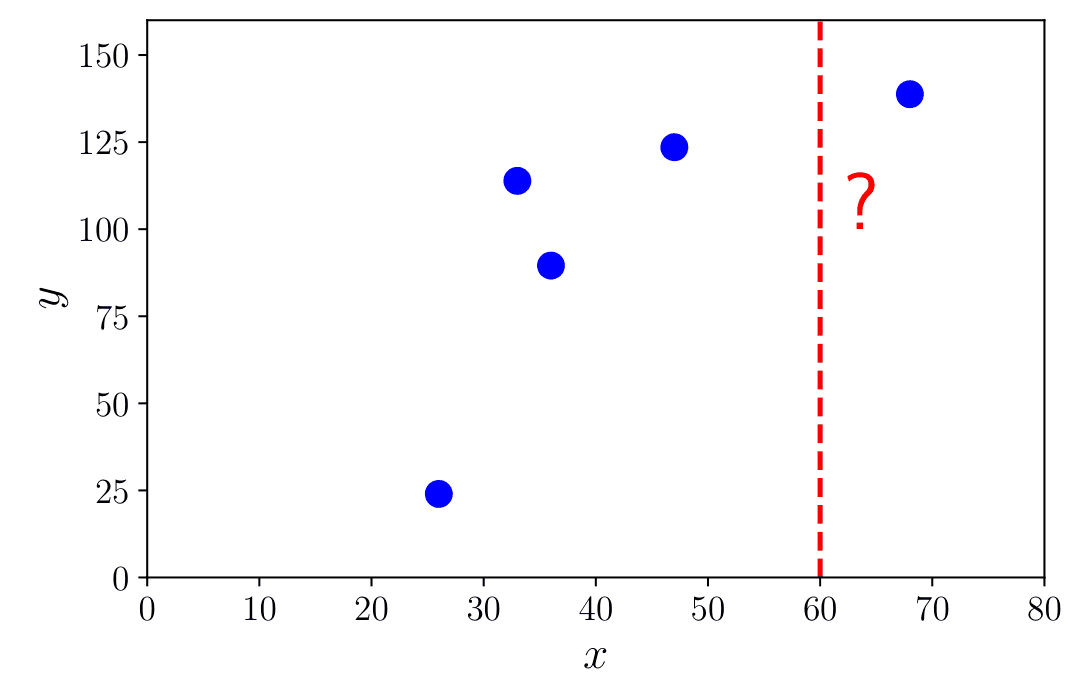
\includegraphics[width=0.92\textwidth,keepaspectratio]{docs/images/Figure8.1.png}
\caption*{\refstepcounter{figcounter}\label{fig:8-1}图~\thefigcounter}
\end{figure}


我们利用本书第一部分介绍的概念将诸如前段所述的机器学习问题形式化。将数据表示为向量 $ \boldsymbol{x}_n $ 使我们能够运用线性代数中的概念（在第 2 章中介绍）。在许多机器学习算法中，我们还需要能够比较两个向量。正如我们将在第 9 章和第 12 章中看到的，计算两个样本之间的相似度或距离使我们能够形式化这一直觉：具有相似特征的样本应该具有相似的标签。两个向量的比较需要我们构建某种几何结构（在第 3 章中解释），并允许我们利用第 7 章的技术对得到的学习问题进行优化。

由于我们将数据表示为向量，我们可以操纵数据以寻找其潜在更优的表示。我们将从两个方面探讨寻找良好表示的方法：寻找原始特征向量的低维近似，以及利用原始特征向量的非线性高维组合。在第 10 章中，我们将看到通过寻找主成分来得到原始数据空间低维近似的示例。寻找主成分与第 4 章中介绍的特征值和奇异值分解概念密切相关。对于高维表示，我们将看到一个显式特征映射 $ \phi(\cdot) $，它允许我们使用更高维的表示 $ \phi(\boldsymbol{x}_n) $ 来表示输入 $ \boldsymbol{x}_n $。高维表示的主要动机在于，我们可以将新特征构建为原始特征的非线性组合，这反过来可能使学习问题变得更容易。我们将在 9.2 节讨论特征映射，并在 12.4 节展示该特征映射如何引出 \emph{核（kernel）} 。近年来，深度学习方法（Goodfellow et al., 2016）在利用数据本身学习新的优质特征方面展现出巨大潜力，并在计算机视觉、语音识别和自然语言处理等领域取得了巨大成功。我们在本书的这部分内容中不涵盖神经网络，但读者可参阅 5.6 节了解反向传播的数学描述，这是训练神经网络的核心概念。

\medskip\hrule\medskip

\section*{8.1.2 作为函数的模型}
\addcontentsline{toc}{subsection}{8.1.2 作为函数的模型}

一旦我们将数据表示为适当的向量形式，就可以着手构建预测函数（称为 \emph{预测器（predictor）}）。在第 1 章中，我们尚未具备精确描述模型的语言。利用本书第一部分的概念，我们现在可以介绍“模型”的具体含义。我们在本书中介绍两种主要方法：将预测器视为函数，以及将预测器视为概率模型。我们在本小节描述前者，在下一小节描述后者。

预测器是一个函数，当给定特定的输入样本（在我们的情况下为一个特征向量）时，产生一个输出。目前，我们考虑输出为一个单一数字，即实值标量输出。这可以写作：

\begin{equation}
f : \mathbb{R}^D \to \mathbb{R}
\tag{8.1}\label{eq:8-1}
\end{equation}

其中输入向量 $ \boldsymbol{x} $ 是 $ D $ 维的（具有 $ D $ 个特征），应用于它的函数 $ f $（写作 $ f(\boldsymbol{x}) $）返回一个实数。图~\ref{fig:8-2} 展示了一个可用于计算输入值 $ x $ 对应预测值的可能函数。


\begin{figure}[H]
\centering
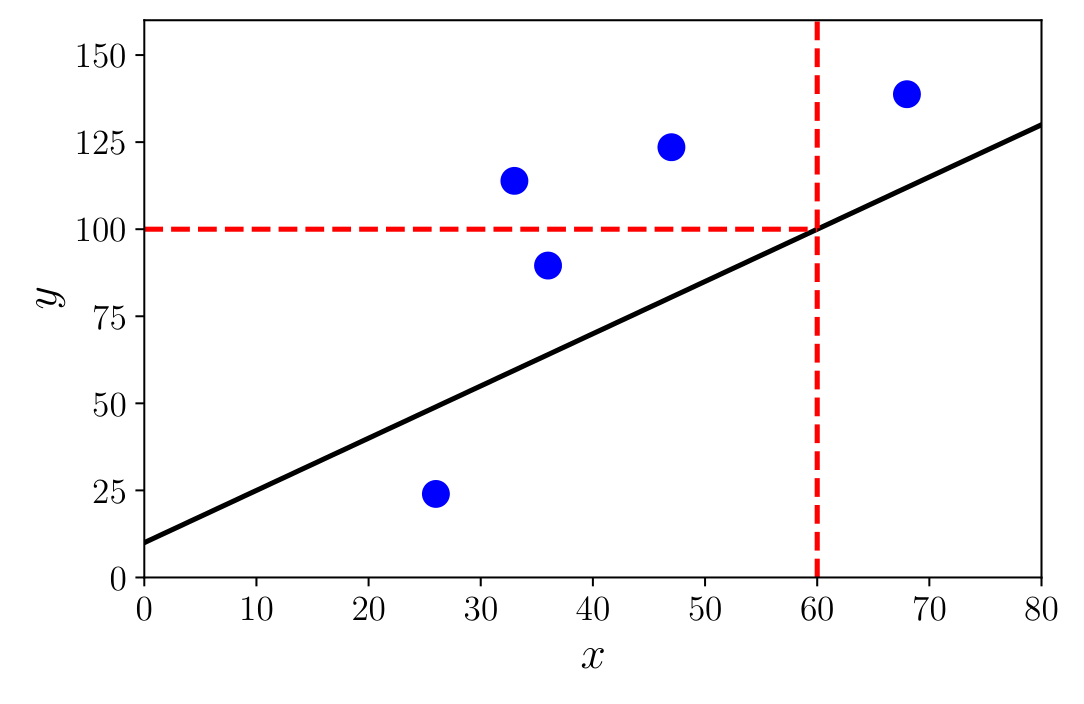
\includegraphics[width=0.92\textwidth,keepaspectratio]{docs/images/Figure8.2.png}
\caption*{\refstepcounter{figcounter}\label{fig:8-2}图~\thefigcounter}
\end{figure}


在本书中，我们不考虑所有函数的一般情形，那将需要泛函分析的知识。相反，我们考虑线性函数的特殊情形：

\begin{equation}
f(\boldsymbol{x}) = \boldsymbol{\theta}^\top \boldsymbol{x} + \theta_0
\tag{8.2}\label{eq:8-2}
\end{equation}

其中 $ \boldsymbol{\theta} $ 和 $ \theta_0 $ 为未知参数。这种限制意味着第 2 章和第 3 章的内容足以精确阐明机器学习非概率视角（相对于下文描述的概率视角）下的预测器概念。线性函数在可解决问题的一般性与所需基础数学知识量之间取得了良好的平衡。

\medskip\hrule\medskip

\section*{8.1.3 作为概率分布的模型}
\addcontentsline{toc}{subsection}{8.1.3 作为概率分布的模型}

我们常常认为数据是对某种真实潜在效应的带噪观测，并希望通过应用机器学习能够从噪声中识别出信号。这要求我们具备量化噪声影响的语言。我们通常还希望预测器能够表达某种不确定性，例如量化我们对特定测试数据点的预测值的置信度。正如我们在第 6 章中所见，概率论提供了量化不确定性的语言。图~\ref{fig:8-3} 将该函数的预测不确定性展示为一个高斯分布。


\begin{figure}[H]
\centering
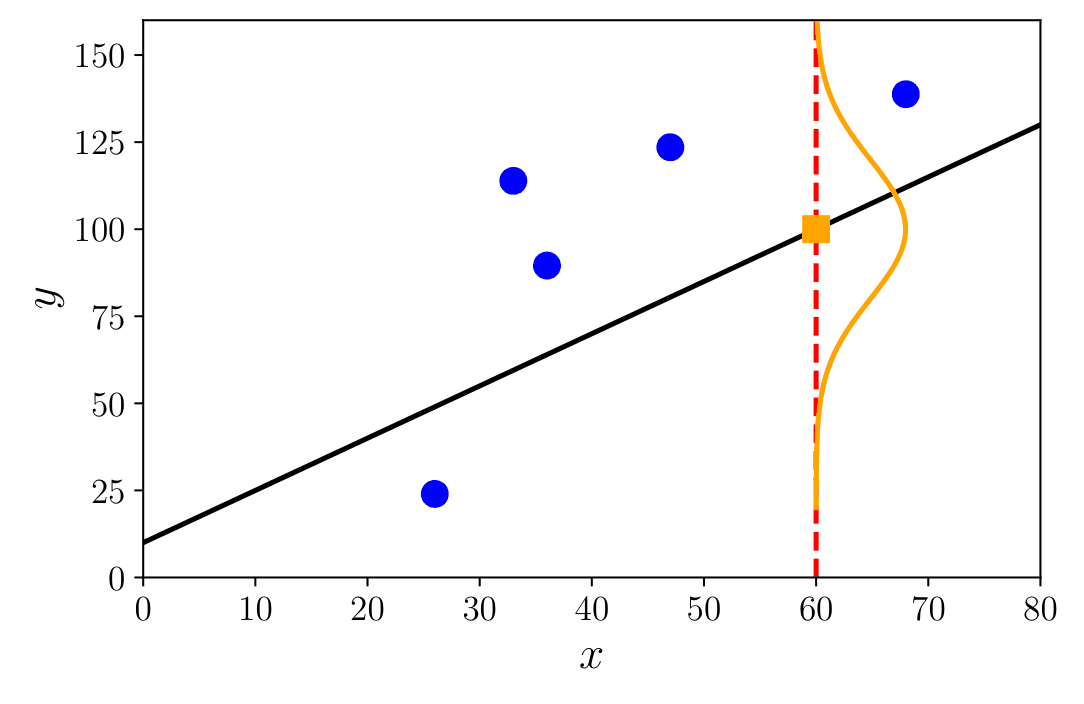
\includegraphics[width=0.92\textwidth,keepaspectratio]{docs/images/Figure8.3.png}
\caption*{\refstepcounter{figcounter}\label{fig:8-3}图~\thefigcounter}
\end{figure}


我们可以不将预测器视为单个函数，而是将预测器视为概率模型，即描述可能函数分布的模型。在本书中，我们仅限于具有有限维参数的分布这一特殊情形，这使我们能够在不需要随机过程和随机测度的情况下描述概率模型。对于这种特殊情形，我们可以将概率模型视为多元概率分布，这已经允许构建非常丰富的模型类别。

我们将在 8.4 节介绍如何利用概率概念（第 6 章）来定义机器学习模型，并在 8.5 节介绍一种以紧凑方式描述概率模型的图语言。

\medskip\hrule\medskip

\section*{8.1.4 学习即寻找参数}
\addcontentsline{toc}{subsection}{8.1.4 学习即寻找参数}

学习的目标是找到一个模型及其对应的参数，使得得到的预测器在未见过的数据上表现良好。在讨论机器学习算法时，概念上有三个截然不同的算法阶段：

\begin{enumerate}
\item \textbf{预测或推断}（Prediction or inference）
\item \textbf{训练或参数估计}（Training or parameter estimation）
\item \textbf{超参数调优或模型选择}（Hyperparameter tuning or model selection）
\end{enumerate}

预测阶段是指我们在之前未见过的测试数据上使用训练好的预测器。换句话说，此时参数和模型选择已经固定，预测器应用于表示新输入数据点的新向量。正如第 1 章和前一小节所述，我们将在本书中探讨机器学习的两大流派，分别对应预测器是函数还是概率模型。当我们拥有概率模型（在 8.4 节中进一步讨论）时，预测阶段被称为 \emph{推断（inference）} 。

\begin{notebox}
\textbf{备注} 遗憾的是，不同的算法阶段并没有公认统一的命名。单词“推断”（inference）有时也被用来表示概率模型的参数估计，而在较少情况下也可用于表示非概率模型的预测。
\end{notebox}

训练或参数估计阶段是指我们根据训练数据调整预测模型的阶段。我们希望在给定训练数据的情况下找到优秀的预测器，为此有两种主要策略：基于某种质量度量寻找最佳预测器（有时称为寻找 \emph{点估计（point estimate）}），或使用贝叶斯推断。寻找点估计可以应用于这两种类型的预测器，但贝叶斯推断需要概率模型。

对于非概率模型，我们遵循 \emph{经验风险最小化（empirical risk minimization）} 原则，这将在 8.2 节中介绍。经验风险最小化直接为寻找良好参数提供了一个优化问题。对于统计模型，通常使用 \emph{极大似然（maximum likelihood）} 原则来寻找一组优秀的参数（8.3 节）。我们还可以使用概率模型对参数的不确定性进行建模，这将在 8.4 节中更详细地探讨。

我们使用数值方法来寻找与数据“拟合”的良好参数，大多数训练方法都可以看作是寻找目标函数最大值（例如极大似然）的爬山算法（hill-climbing）。为了应用爬山方法，我们使用第 5 章中描述的梯度，并实现第 7 章中的数值优化方法。

\begin{notebox}
\textbf{提示} 优化领域的惯例是最小化目标函数。因此，在机器学习目标函数中常常会多出一个负号。
\end{notebox}

正如第 1 章所述，我们感兴趣的是基于数据学习一个模型，使其在未来的数据上表现良好。仅在训练数据上拟合良好是不够的，预测器需要在未见数据上表现良好。我们使用 \emph{交叉验证（cross-validation）} （8.2.4 节）来模拟预测器在未来未见数据上的表现。正如我们将在本章看到的，为了实现对未见数据表现良好的目标，我们需要在良好拟合训练数据与寻找现象的“简单”解释之间进行权衡。这种权衡是通过使用 \emph{正则化（regularization）} （8.2.3 节）或添加 \emph{先验（prior）} （8.3.2 节）来实现的。在哲学上，这既不被视为归纳（induction），也不被视为演绎（deduction），而是被称为 \emph{溯因（abduction）} 。根据《斯坦福哲学百科全书》，溯因是指“推向最佳解释的推断过程”（Douven, 2017）。

我们常常需要对预测器的结构做出高层次的建模决策，例如要使用的组件数量或要考虑的概率分布类别。组件数量的选择是 \emph{超参数（hyperparameter）} 的一个例子，这种选择会显著影响模型的性能。在不同模型之间进行选择的问题称为 \emph{模型选择（model selection）} ，我们将在 8.6 节中进行介绍。对于非概率模型，模型选择通常使用 \emph{嵌套交叉验证（nested cross-validation）} 进行，这将在 8.6.1 节中介绍。我们还利用模型选择来挑选模型的超参数。

\begin{notebox}
\textbf{备注} 参数与超参数之间的界限有些随意，主要取决于什么可以通过数值直接优化，与什么需要采用搜索技术。理解这一区别的另一种视角是将参数视为概率模型的显式参数，并将超参数（更高层级的参数）视为控制这些显式参数分布的参数。
\end{notebox}

在接下来的各节中，我们将考察机器学习的三种风格：经验风险最小化（8.2 节）、极大似然原理（8.3 节）以及概率建模（8.4 节）。

\section*{8.2 经验风险最小化}
\addcontentsline{toc}{section}{8.2 经验风险最小化}
\label{sec:8.2}

在掌握了所有的数学基础之后，我们现在可以阐明什么是“学习”了。机器学习中的“学习”部分归结为基于训练数据估计参数。在本节中，我们考虑预测器是一个函数的情形，并在 8.3 节中考虑概率模型的情形。我们在此描述 \emph{经验风险最小化（empirical risk minimization）} 的思想，该思想最初因支持向量机的提出（在第 12 章中描述）而广为人知。然而，它的一般原则具有广泛的适用性，使我们能够在不显式构建概率模型的情况下探讨什么是学习。这里有四个主要的设计选择，我们将在接下来的小节中详细讨论：

\begin{itemize}
\item 8.2.1 节：我们允许预测器采用的函数集合是什么？
\item 8.2.2 节：我们如何度量预测器在训练数据上的表现优劣？
\item 8.2.3 节：我们如何仅从训练数据构建出在未见过的测试数据上表现良好的预测器？
\item 8.2.4 节：在模型空间中进行搜索的具体流程是什么？
\end{itemize}

\medskip\hrule\medskip

\section*{8.2.1 假设函数类}
\addcontentsline{toc}{subsection}{8.2.1 假设函数类}

假设给定 $ N $ 个样本 $ \boldsymbol{x}_n \in \mathbb{R}^D $ 及对应的标量标签 $ y_n \in \mathbb{R} $。我们考虑监督学习设定，其中获取到数据对 $ (\boldsymbol{x}_1, y_1), \ldots, (\boldsymbol{x}_N, y_N) $。给定这些数据，我们希望估计一个由 $ \boldsymbol{\theta} $ 参数化的预测器 $ f(\cdot, \boldsymbol{\theta}) : \mathbb{R}^D \to \mathbb{R} $。我们希望能够找到一个优秀的参数 $ \boldsymbol{\theta}^* $，使得模型能很好地拟合数据，即：

\begin{equation}
f(\boldsymbol{x}_n, \boldsymbol{\theta}^*) \approx y_n \quad \textcn{对所有 } n = 1, \ldots, N
\tag{8.3}\label{eq:8-3}
\end{equation}

在本节中，我们使用记号 $ \hat{y}_n = f(\boldsymbol{x}_n, \boldsymbol{\theta}^*) $ 表示预测器的输出。

\begin{notebox}
\textbf{备注} 为便于阐述，我们将基于监督学习（具有标签的场景）来描述经验风险最小化。这简化了假设类和损失函数的定义。在机器学习中，选择参数化函数类（例如仿射函数）也是非常普遍的做法。
\end{notebox}

\subsection*{例 8.1}
\addcontentsline{toc}{subsubsection}{例 8.1}

我们引入普通最小二乘回归问题来说明经验风险最小化。关于回归的更全面论述见第 9 章。当标签 $ y_n $ 为实数值时，预测器函数类的一个流行选择是仿射函数集。在机器学习中，仿射函数通常也被称为线性函数。我们可以通过在 $ \boldsymbol{x}_n $ 上拼接一个额外的单位特征 $ x_n^{(0)} = 1 $ 来采用更紧凑的记号表示仿射函数，即 $ \boldsymbol{x}_n = [1, x_n^{(1)}, x_n^{(2)}, \ldots, x_n^{(D)}]^\top $。对应的参数向量为 $ \boldsymbol{\theta} = [\theta_0, \theta_1, \theta_2, \ldots, \theta_D]^\top $，这使我们能够将预测器写成线性函数形式：

\begin{equation}
f(\boldsymbol{x}_n, \boldsymbol{\theta}) = \boldsymbol{\theta}^\top \boldsymbol{x}_n
\tag{8.4}\label{eq:8-4}
\end{equation}

该线性预测器等价于仿射模型：

\begin{equation}
f(\boldsymbol{x}_n, \boldsymbol{\theta}) = \theta_0 + \sum_{d=1}^D \theta_d x_n^{(d)}
\tag{8.5}\label{eq:8-5}
\end{equation}

预测器接收表示单个样本的特征向量 $ \boldsymbol{x}_n $ 作为输入，并产生一个实数值输出，即 $ f : \mathbb{R}^{D+1} \to \mathbb{R} $。本章前面的示意图均以直线作为预测器，这意味着我们假设了仿射函数。

除线性函数外，我们也可以考虑非线性函数作为预测器。神经网络领域的最新进展使得对更复杂的非线性函数类进行高效计算成为可能。

在确定了函数类别之后，我们希望搜索到一个优秀的预测器。现在我们进入经验风险最小化的第二个核心要素：如何度量预测器与训练数据的拟合优劣。

\medskip\hrule\medskip

\section*{8.2.2 用于训练的损失函数}
\addcontentsline{toc}{subsection}{8.2.2 用于训练的损失函数}

考虑特定样本的真实标签 $ y_n $，以及我们基于 $ \boldsymbol{x}_n $ 做出的对应预测 $ \hat{y}_n $。为了定义何为与数据“拟合良好”，我们需要指定一个 \emph{损失函数（loss function）} $ \ell(y_n, \hat{y}_n) $，它以真实标签和预测值为输入，并产生一个非负实数（称为 \emph{损失（loss）}），表示我们在该特定预测上产生了多少误差。“误差”（error）这一表达通常被用来指代损失。我们寻找优秀参数向量 $ \boldsymbol{\theta}^* $ 的目标是最小化在 $ N $ 个训练样本集上的平均损失。

机器学习中常做的一个假设是样本集合 $ (\boldsymbol{x}_1, y_1), \ldots, (\boldsymbol{x}_N, y_N) $ 是 \emph{独立同分布（independent and identically distributed, i.i.d.）} 的。词语“独立”（6.4.5 节）意味着两个数据点 $ (\boldsymbol{x}_i, y_i) $ 与 $ (\boldsymbol{x}_j, y_j) $ 在统计上互不依赖，这保证了经验均值是总体均值（6.4.1 节）的优良估计。这意味着我们可以使用训练数据上损失的经验均值。对于给定的 \emph{训练集（training set）} $ \{(\boldsymbol{x}_1, y_1), \ldots, (\boldsymbol{x}_N, y_N)\} $，我们引入样本矩阵 $ \boldsymbol{X} := [\boldsymbol{x}_1, \ldots, \boldsymbol{x}_N]^\top \in \mathbb{R}^{N \times D} $ 和标签向量 $ \boldsymbol{y} := [y_1, \ldots, y_N]^\top \in \mathbb{R}^N $ 的记号。利用该矩阵记号，平均损失由下式给出：

\begin{equation}
R_{\text{emp}}(f, \boldsymbol{X}, \boldsymbol{y}) = \frac{1}{N} \sum_{n=1}^N \ell(y_n, \hat{y}_n)
\tag{8.6}\label{eq:8-6}
\end{equation}

其中 $ \hat{y}_n = f(\boldsymbol{x}_n, \boldsymbol{\theta}) $。式~\eqref{eq:8-6} 被称为 \emph{经验风险（empirical risk）} ，它取决于三个参数：预测器 $ f $ 以及数据 $ \boldsymbol{X}, \boldsymbol{y} $。这种学习的一般策略被称为 \emph{经验风险最小化（empirical risk minimization）} 。

\subsection*{例 8.2（最小二乘损失）}
\addcontentsline{toc}{subsubsection}{例 8.2（最小二乘损失）}

继续最小二乘回归的例子，我们规定在训练期间使用平方损失 $ \ell(y_n, \hat{y}_n) = (y_n - \hat{y}_n)^2 $ 来度量犯错的代价。我们希望最小化经验风险 (8.6)，即数据上损失的均值：

\begin{equation}
\min_{\boldsymbol{\theta} \in \mathbb{R}^D} \frac{1}{N} \sum_{n=1}^N \left(y_n - f(\boldsymbol{x}_n, \boldsymbol{\theta})\right)^2
\tag{8.7}\label{eq:8-7}
\end{equation}

其中代入了预测器 $ \hat{y}_n = f(\boldsymbol{x}_n, \boldsymbol{\theta}) $。通过采用线性预测器 $ f(\boldsymbol{x}_n, \boldsymbol{\theta}) = \boldsymbol{\theta}^\top \boldsymbol{x}_n $，我们得到优化问题：

\begin{equation}
\min_{\boldsymbol{\theta} \in \mathbb{R}^D} \frac{1}{N} \sum_{n=1}^N \left(y_n - \boldsymbol{\theta}^\top \boldsymbol{x}_n\right)^2 .
\tag{8.8}\label{eq:8-8}
\end{equation}

该方程可以等价地表示为矩阵形式：

\begin{equation}
\min_{\boldsymbol{\theta} \in \mathbb{R}^D} \frac{1}{N} \|\boldsymbol{y} - \boldsymbol{X}\boldsymbol{\theta}\|^2 .
\tag{8.9}\label{eq:8-9}
\end{equation}

这被称为 \emph{最小二乘问题（least-squares problem）} 。通过求解正规方程组（normal equations），该问题存在闭式解析解，我们将在 9.2 节中详细讨论。

我们感兴趣的不是仅仅在训练数据上表现优异的预测器，而是寻求在未见过的测试数据上表现出色（具有低风险）的预测器。更形式化地，我们感兴趣的是寻找一个预测器 $ f $（参数固定），使其最小化 \emph{期望风险（expected risk）} ：

\begin{equation}
R_{\text{true}}(f) = \mathbb{E}_{\boldsymbol{x}, y}[\ell(y, f(\boldsymbol{x}))]
\tag{8.10}\label{eq:8-10}
\end{equation}

其中 $ y $ 为标签，$ f(\boldsymbol{x}) $ 为基于样本 $ \boldsymbol{x} $ 做出的预测。记号 $ R_{\text{true}}(f) $ 表示如果我们拥有无限量数据时的真实风险。常用于指代期望风险的另一个短语是“总体风险”（population risk）。期望是在所有可能数据和标签的（无限）集合上取的。由最小化期望风险的愿望引发了两个实际问题，我们将在接下来的两个小节中分别予以解决：

\begin{itemize}
\item 我们应该如何调整训练过程以实现良好的泛化？
\item 我们如何从（有限的）数据中估计期望风险？
\end{itemize}

\begin{notebox}
\textbf{备注} 许多机器学习任务在设定时都会关联一个性能度量指标，例如预测准确率或均方根误差。该性能指标可能更为复杂，具有成本敏感性，并能捕捉具体应用的细节。原则上，经验风险最小化的损失函数设计应当直接对应于机器学习任务所规定的性能指标。然而在实践中，损失函数的设计与最终的性能指标之间往往存在不匹配。这可能是由于便于实现或优化效率等实际考量所导致的。
\end{notebox}

\medskip\hrule\medskip

\section*{8.2.3 降低过拟合的正则化}
\addcontentsline{toc}{subsection}{8.2.3 降低过拟合的正则化}

本小节介绍经验风险最小化的一个补充扩展，使其能够良好泛化（近似最小化期望风险）。回想一下，训练机器学习预测器的目标是使其在未见数据上表现良好，即预测器具有优良的 \emph{泛化能力（generalizes well）} 。我们通过从整个数据集中保留出一部分来模拟这种未见数据。这个保留出来的集合被称为 \emph{测试集（test set）} 。即便仅仅获知预测器在测试集上的性能，也会造成信息泄漏（Blum and Hardt, 2015）。给定足够丰富的预测器函数类 $ f $，我们基本上可以通过完全“记住”训练数据来获得零经验风险。虽然这对于最小化训练数据上的损失（从而最小化风险）非常有效，但我们不能期望该预测器能够很好地泛化到未见数据。在实践中，我们只有有限的数据集，因此我们将数据划分为训练集和测试集。训练集用于拟合模型，而测试集（在训练期间不被机器学习算法所见）用于评估泛化性能。对于使用者来说，在观察到测试集的结果后切忌掉头返回并展开新一轮训练，这一点至关重要。我们分别使用下标 $ \text{train} $ 和 $ \text{test} $ 表示训练集和测试集。我们将在 8.2.4 节重温利用有限数据集评估期望风险的思想。

事实证明，经验风险最小化可能导致 \emph{过拟合（overfitting）} ，即预测器与训练数据拟合得过于紧密，而无法很好地泛化到新数据（Mitchell, 1997）。在训练集上平均损失极小但在测试集上平均损失巨大的普遍现象，往往发生在我们拥有较少数据且假设类过于复杂的情况下。对于某个特定的预测器 $ f $（参数已固定），当来自训练数据的风险估计 $ R_{\text{emp}}(f, \boldsymbol{X}_{\text{train}}, \boldsymbol{y}_{\text{train}}) $ 低估了期望风险 $ R_{\text{true}}(f) $ 时，就会发生过拟合现象。由于我们通过使用测试集上的经验风险 $ R_{\text{emp}}(f, \boldsymbol{X}_{\text{test}}, \boldsymbol{y}_{\text{test}}) $ 来估计期望风险 $ R_{\text{true}}(f) $，因此若测试风险远大于训练风险，便表明发生了过拟合。我们将在 8.3.3 节中重温过拟合的概念。

因此，我们需要通过引入惩罚项在某种程度上对经验风险极小化值的搜索施加偏置，从而使优化器更难返回过于灵活的预测器。在机器学习中，该惩罚项被称为 \emph{正则化（regularization）} 。正则化是一种在经验风险最小化的精确解与解的规模或复杂度之间达成折衷的方法。

\subsection*{例 8.3（正则化最小二乘）}
\addcontentsline{toc}{subsubsection}{例 8.3（正则化最小二乘）}

正则化是一种抑制优化问题出现复杂或极端解的方法。最简单的正则化策略是通过添加一个仅涉及 $ \boldsymbol{\theta} $ 的惩罚项，将前例中的最小二乘问题：

\begin{equation}
\min_{\boldsymbol{\theta}} \frac{1}{N} \|\boldsymbol{y} - \boldsymbol{X}\boldsymbol{\theta}\|^2
\tag{8.11}\label{eq:8-11}
\end{equation}

替换为“正则化”问题：

\begin{equation}
\min_{\boldsymbol{\theta}} \frac{1}{N} \|\boldsymbol{y} - \boldsymbol{X}\boldsymbol{\theta}\|^2 + \lambda \|\boldsymbol{\theta}\|^2 .
\tag{8.12}\label{eq:8-12}
\end{equation}

附加项 $ \|\boldsymbol{\theta}\|^2 $ 被称为 \emph{正则化子（regularizer）} ，参数 $ \lambda $ 为 \emph{正则化参数（regularization parameter）} 。正则化参数权衡了最小化训练集上的损失与参数 $ \boldsymbol{\theta} $ 的幅值大小。如果发生过拟合，参数值的大小往往会变得相当庞大（Bishop, 2006）。

正则化项有时也被称为 \emph{惩罚项（penalty term）} ，它将向量 $ \boldsymbol{\theta} $ 偏置向靠近原点的方向。正则化的思想也以参数的先验概率形式出现在概率模型中。回想 6.6 节，为了使后验分布与先验分布具有相同的形式，先验分布与似然函数必须是共轭的。我们将在 8.3.2 节中重新审视这一思想。在第 12 章中我们还将看到，正则化子的思想在几何上等价于大间隔（large margin）的思想。

\medskip\hrule\medskip

\section*{8.2.4 评估泛化性能的交叉验证}
\addcontentsline{toc}{subsection}{8.2.4 评估泛化性能的交叉验证}

我们在上一节中提到，我们通过将预测器应用于测试数据来估计泛化误差。这部分保留出来的数据有时也被称为 \emph{验证集（validation set）} 。验证集是我们保留出来的可用训练数据的一个子集。该方法的一个实际问题在于数据量通常有限，而理想情况下我们希望利用尽可能多的可用数据来训练模型。这将要求我们将验证集 $ \mathcal{V} $ 保持得很小，但这反过来又会导致对预测性能的估计产生高方差（噪声很大）。针对这些相互矛盾的目标（既要大训练集，又要大验证集）的一种解决方案是使用 \emph{交叉验证（cross-validation）} 。$ K $ 折交叉验证有效地将数据划分为 $ K $ 个数据块，其中 $ K-1 $ 个数据块构成训练集 $ \mathcal{R} $，最后一个数据块充当验证集 $ \mathcal{V} $（类似于前面概述的思想）。交叉验证（在理想情况下）遍历将数据块分配给 $ \mathcal{R} $ 和 $ \mathcal{V} $ 的所有组合方式；参见图~\ref{fig:8-4}。对验证集的所有 $ K $ 种选择重复此过程，并将来自这 $ K $ 次运行的模型性能取平均。


\begin{figure}[H]
\centering
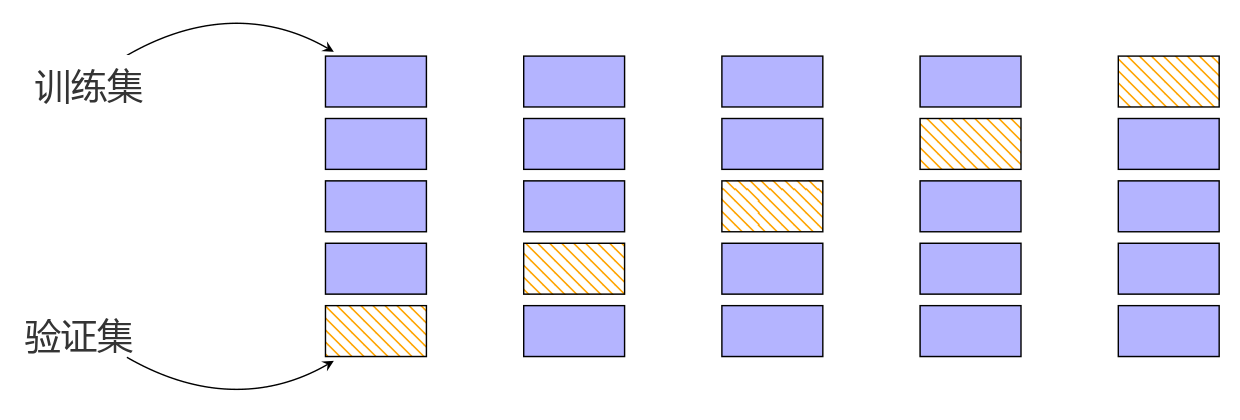
\includegraphics[width=0.92\textwidth,keepaspectratio]{docs/images/Figure8.4.png}
\caption*{\refstepcounter{figcounter}\label{fig:8-4}图~\thefigcounter}
\end{figure}


我们将数据集划分为两个集合 $ \mathcal{D} = \mathcal{R} \cup \mathcal{V} $，使得它们不重叠（$ \mathcal{R} \cap \mathcal{V} = \emptyset $），其中 $ \mathcal{V} $ 为验证集，并在 $ \mathcal{R} $ 上训练模型。训练完成后，我们在验证集 $ \mathcal{V} $ 上评估预测器 $ f $ 的性能（例如，通过计算训练模型在验证集上的均方根误差 RMSE）。更确切地说，对于每个划分 $ k $，训练数据 $ \mathcal{R}^{(k)} $ 产生一个预测器 $ f^{(k)} $，然后将其应用于验证集 $ \mathcal{V}^{(k)} $ 以计算经验风险 $ R(f^{(k)}, \mathcal{V}^{(k)}) $。我们遍历验证集和训练集的所有可能划分，并计算预测器的平均泛化误差。交叉验证近似了期望泛化误差：

\begin{equation}
\mathbb{E}_{\mathcal{V}}[R(f, \mathcal{V})] \approx \frac{1}{K} \sum_{k=1}^K R(f^{(k)}, \mathcal{V}^{(k)})
\tag{8.13}\label{eq:8-13}
\end{equation}

其中 $ R(f^{(k)}, \mathcal{V}^{(k)}) $ 是预测器 $ f^{(k)} $ 在验证集 $ \mathcal{V}^{(k)} $ 上的风险（例如 RMSE）。这种近似有两个误差来源：第一，由于训练集有限，导致生成的 $ f^{(k)} $ 并非可能达到的最佳预测器；第二，由于验证集有限，导致对风险 $ R(f^{(k)}, \mathcal{V}^{(k)}) $ 的估计不够精确。$ K $ 折交叉验证的一个潜在缺点是需要将模型训练 $ K $ 次所带来的计算成本，如果单次训练计算开销很大，这可能会构成沉重负担。在实践中，仅仅考察直接参数往往是不够的。例如，我们需要探索多个复杂度参数（例如多个正则化参数），它们可能并非模型的直接内部参数。依赖于这些超参数来评估模型质量，可能会导致训练运行次数随着模型参数数量呈指数级增长。我们可以使用 \emph{嵌套交叉验证（nested cross-validation）} （8.6.1 节）来搜索优质超参数。

然而，交叉验证是一个 \emph{高度易并行（embarrassingly parallel）} 的问题，即只需极少的协调工作即可将问题分解为若干并行任务。在具备充足计算资源（例如云计算、服务器集群）的情况下，交叉验证所需的时间并不比单次性能评估长。

在本节中，我们看到经验风险最小化基于以下核心概念：函数假设类、损失函数和正则化。在 8.3 节中，我们将看到使用概率分布来替代损失函数和正则化思想所产生的效果。

\medskip\hrule\medskip

\section*{8.2.5 延伸阅读}
\addcontentsline{toc}{subsection}{8.2.5 延伸阅读}

由于经验风险最小化的原始提出（Vapnik, 1998）采用了深奥严谨的理论语言，随后的许多发展也都集中在理论领域。这一研究领域被称为 \emph{统计学习理论（statistical learning theory）} （Vapnik, 1999; Evgeniou et al., 2000; Hastie et al., 2001; von Luxburg and Schölkopf, 2011）。一本建立在理论基础之上并发展了高效学习算法的近期机器学习教科书是 Shalev-Shwartz and Ben-David (2014)。

正则化的概念起源于病态逆问题的求解（Neumaier, 1998）。这里介绍的方法称为 \emph{吉洪诺夫正则化（Tikhonov regularization）} ，还有一个密切相关的约束版本称为 \emph{伊万诺夫正则化（Ivanov regularization）} 。吉洪诺夫正则化与偏差-方差权衡（bias-variance trade-off）以及特征选择具有深刻的内在联系（Bühlmann and Van De Geer, 2011）。交叉验证的替代方法包括自举法（bootstrap）和刀切法（jackknife）（Efron and Tibshirani, 1993; Davidson and Hinkley, 1997; Hall, 1992）。

将经验风险最小化（8.2 节）视为“完全脱离概率”是不准确的。支配数据生成的背后存在一个潜在的未知概率分布 $ p(\boldsymbol{x}, y) $。然而，经验风险最小化方法对该具体分布的选择是不可知的（agnostic）。这与明确要求获知 $ p(\boldsymbol{x}, y) $ 的标准统计方法形成鲜明对比。此外，由于该分布是样本 $ \boldsymbol{x} $ 和标签 $ y $ 的联合分布，因此标签可以是非确定性的。与标准统计学不同，我们不需要为标签 $ y $ 指定显式的噪声分布。

\section*{8.3 参数估计}
\addcontentsline{toc}{section}{8.3 参数估计}
\label{sec:8.3}

在 8.2 节中，我们没有显式地使用概率分布对问题进行建模。在本节中，我们将看到如何利用概率分布对观测过程引起的不确定性以及预测器参数中的不确定性进行建模。在 8.3.1 节中，我们引入似然函数（likelihood），它类似于经验风险最小化中的损失函数概念（8.2.2 节）。先验分布的概念（8.3.2 节）类似于正则化的概念（8.2.3 节）。

\medskip\hrule\medskip

\section*{8.3.1 极大似然估计}
\addcontentsline{toc}{subsection}{8.3.1 极大似然估计}

\emph{极大似然估计（maximum likelihood estimation, MLE）} 的核心思想是定义一个关于参数的函数，使我们能够找到一个能很好拟合数据的模型。估计问题聚焦于似然函数，更确切地说是其负对数。对于由随机变量 $ \boldsymbol{x} $ 表示的数据以及由 $ \boldsymbol{\theta} $ 参数化的概率密度族 $ p(\boldsymbol{x} \mid \boldsymbol{\theta}) $， \emph{负对数似然（negative log-likelihood）} 由下式给出：

\begin{equation}
L_{\boldsymbol{x}}(\boldsymbol{\theta}) = -\log p(\boldsymbol{x} \mid \boldsymbol{\theta}) .
\tag{8.14}\label{eq:8-14}
\end{equation}

记号 $ L_{\boldsymbol{x}}(\boldsymbol{\theta}) $ 强调参数 $ \boldsymbol{\theta} $ 是变量，而数据 $ \boldsymbol{x} $ 是固定的。我们在书写负对数似然时经常省去对 $ \boldsymbol{x} $ 的引用，因为它本质上是关于 $ \boldsymbol{\theta} $ 的函数；当表示数据不确定性的随机变量在上下文中清晰明确时，我们简记为 $ L(\boldsymbol{\theta}) $。

让我们解释一下对于固定的 $ \boldsymbol{\theta} $ 值，概率密度 $ p(\boldsymbol{x} \mid \boldsymbol{\theta}) $ 究竟建模了什么。它是一个用于对数据的不确定性建模的分布。换句话说，一旦我们选定了作为预测器的函数类型，似然函数就给出了观测到数据 $ \boldsymbol{x} $ 的概率。

从互补的视角来看，如果我们认为数据是固定的（因为它们已经被观测到），而改变参数 $ \boldsymbol{\theta} $，那么 $ L(\boldsymbol{\theta}) $ 告诉了我们什么？它告诉我们对于这组观测 $ \boldsymbol{x} $，特定的 $ \boldsymbol{\theta} $ 设置有多大的“可能性”（how likely）。基于这第二种视角，极大似然估计器给出了对于该数据集最可能的参数 $ \boldsymbol{\theta} $。

我们考虑监督学习设定，其中获取到数据对 $ (\boldsymbol{x}_1, y_1), \ldots, (\boldsymbol{x}_N, y_N) $，其中 $ \boldsymbol{x}_n \in \mathbb{R}^D $ 且标签 $ y_n \in \mathbb{R} $。我们感兴趣的是构建一个预测器，该预测器接收特征向量 $ \boldsymbol{x}_n $ 作为输入并产生预测 $ y_n $（或接近它的值），即给定向量 $ \boldsymbol{x}_n $，我们希望获得标签 $ y_n $ 的概率分布。换句话说，我们在特定参数设置 $ \boldsymbol{\theta} $ 下指定给定样本时标签的条件概率分布。

\subsection*{例 8.4}
\addcontentsline{toc}{subsubsection}{例 8.4}

常用的第一个例子是指定给定样本时标签的条件概率服从高斯分布。换句话说，我们假设可以用均值为零的独立高斯噪声（参见 6.5 节）$ \varepsilon_n \sim \mathcal{N}(0, \sigma^2) $ 来解释观测不确定性。我们进一步假设使用线性模型 $ \boldsymbol{x}_n^\top \boldsymbol{\theta} $ 进行预测。这意味着我们为每个“样本-标签”对 $ (\boldsymbol{x}_n, y_n) $ 指定一个高斯似然：

\begin{equation}
p(y_n \mid \boldsymbol{x}_n, \boldsymbol{\theta}) = \mathcal{N}\left(y_n \mid \boldsymbol{x}_n^\top \boldsymbol{\theta}, \sigma^2\right) .
\tag{8.15}\label{eq:8-15}
\end{equation}

图~\ref{fig:8-3} 展示了给定参数 $ \boldsymbol{\theta} $ 下的高斯似然示意。我们将在 9.2 节中看到如何根据高斯分布将上述表达式显式展开。

我们假设样本集合 $ (\boldsymbol{x}_1, y_1), \ldots, (\boldsymbol{x}_N, y_N) $ 是独立同分布（i.i.d.）的。“独立”（6.4.5 节）意味着整个数据集（$ \mathcal{Y} = \{y_1, \ldots, y_N\} $ 与 $ \mathcal{X} = \{\boldsymbol{x}_1, \ldots, \boldsymbol{x}_N\} $）的似然可以分解为每个单独样本似然的乘积：

\begin{equation}
p(\mathcal{Y} \mid \mathcal{X}, \boldsymbol{\theta}) = \prod_{n=1}^N p(y_n \mid \boldsymbol{x}_n, \boldsymbol{\theta})
\tag{8.16}\label{eq:8-16}
\end{equation}

其中 $ p(y_n \mid \boldsymbol{x}_n, \boldsymbol{\theta}) $ 是某个特定分布（在例 8.4 中为高斯分布）。“同分布”意味着式~\eqref{eq:8-16} 中乘积的每一项服从相同的分布形式，并且它们共享相同的参数。从优化的角度来看，计算可以分解为较简单函数之和的函数通常更容易。因此，在机器学习中我们经常考虑负对数似然（回想 $ \log(ab) = \log(a) + \log(b) $）：

\begin{equation}
L(\boldsymbol{\theta}) = -\log p(\mathcal{Y} \mid \mathcal{X}, \boldsymbol{\theta}) = -\sum_{n=1}^N \log p(y_n \mid \boldsymbol{x}_n, \boldsymbol{\theta}) .
\tag{8.17}\label{eq:8-17}
\end{equation}

虽然在式~\eqref{eq:8-15} 的 $ p(y_n \mid \boldsymbol{x}_n, \boldsymbol{\theta}) $ 中，容易诱人地将位于条件符号右侧的 $ \boldsymbol{\theta} $ 解释为已观测且固定的量，但这种理解是不正确的。负对数似然 $ L(\boldsymbol{\theta}) $ 是关于 $ \boldsymbol{\theta} $ 的函数。因此，为了找到一个能够很好解释数据 $ (\boldsymbol{x}_1, y_1), \ldots, (\boldsymbol{x}_N, y_N) $ 的优质参数向量 $ \boldsymbol{\theta} $，我们关于 $ \boldsymbol{\theta} $ 最小化负对数似然 $ L(\boldsymbol{\theta}) $。

\begin{notebox}
\textbf{备注} 式~\eqref{eq:8-17} 中的负号是一个历史沿革的产物：我们通常希望最大化似然，但数值优化文献普遍习惯于研究函数的最小化问题。
\end{notebox}

\subsection*{例 8.5}
\addcontentsline{toc}{subsubsection}{例 8.5}

继续我们关于高斯似然的例子 (8.15)，负对数似然可以重写为：

\begin{equation}
L(\boldsymbol{\theta}) = -\sum_{n=1}^N \log p(y_n \mid \boldsymbol{x}_n, \boldsymbol{\theta}) = -\sum_{n=1}^N \log \mathcal{N}\left(y_n \mid \boldsymbol{x}_n^\top \boldsymbol{\theta}, \sigma^2\right)
\tag{8.18a}\label{eq:8-18a}
\end{equation}

\begin{equation}
= -\sum_{n=1}^N \log \left( \frac{1}{\sqrt{2\pi\sigma^2}} \exp\left( -\frac{(y_n - \boldsymbol{x}_n^\top \boldsymbol{\theta})^2}{2\sigma^2} \right) \right)
\tag{8.18b}\label{eq:8-18b}
\end{equation}

\begin{equation}
= -\sum_{n=1}^N \log \exp\left( -\frac{(y_n - \boldsymbol{x}_n^\top \boldsymbol{\theta})^2}{2\sigma^2} \right) - \sum_{n=1}^N \log \frac{1}{\sqrt{2\pi\sigma^2}}
\tag{8.18c}\label{eq:8-18c}
\end{equation}

\begin{equation}
= \frac{1}{2\sigma^2} \sum_{n=1}^N (y_n - \boldsymbol{x}_n^\top \boldsymbol{\theta})^2 - \sum_{n=1}^N \log \frac{1}{\sqrt{2\pi\sigma^2}} .
\tag{8.18d}\label{eq:8-18d}
\end{equation}

由于 $ \sigma $ 是给定的，式~\eqref{eq:8-18d} 中的第二项是常数，因此最小化 $ L(\boldsymbol{\theta}) $ 严格对应于求解第一项所表达的最小二乘问题（与式~\eqref{eq:8-8} 比较）。

事实证明，对于高斯似然，对应于极大似然估计的优化问题具有闭式解。我们将在第 9 章中看到更多细节。图~\ref{fig:8-5} 展示了一个回归数据集以及由极大似然参数所诱导出的函数。类似于未正则化的经验风险最小化（9.2.3 节），极大似然估计也可能遭受过拟合（8.3.3 节）。对于其他似然函数，即如果我们用非高斯分布对噪声进行建模，极大似然估计可能不具备闭式解析解。在这种情况下，我们求助于第 7 章中讨论的数值优化方法。


\begin{figure}[H]
\centering
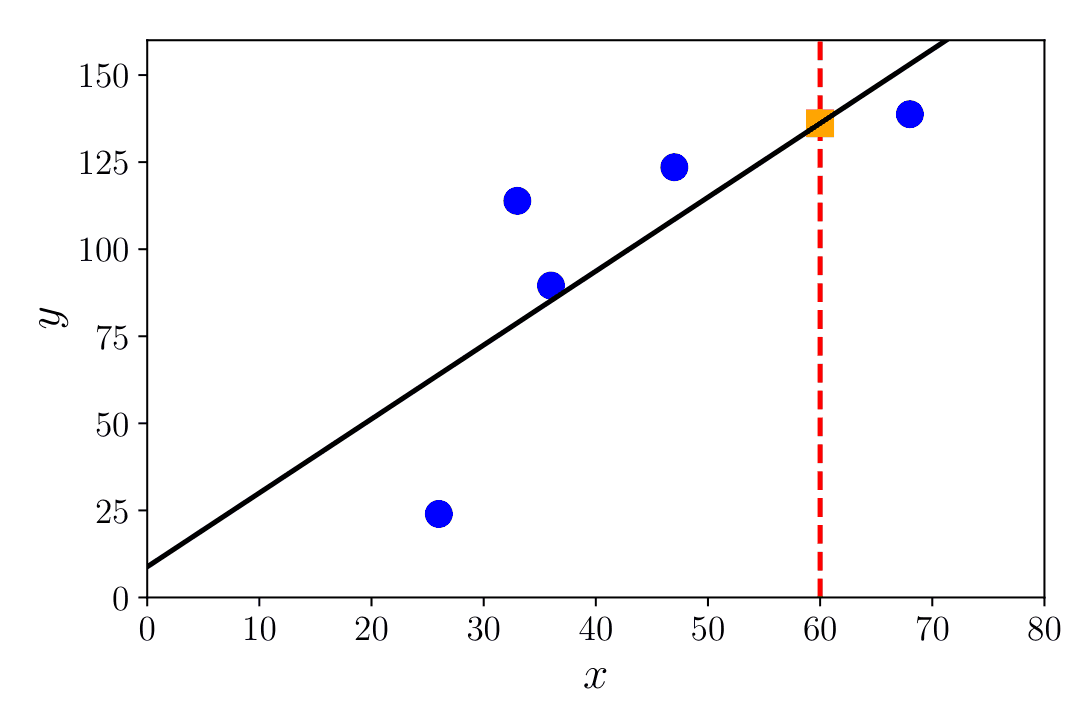
\includegraphics[width=0.92\textwidth,keepaspectratio]{docs/images/Figure8.5.png}
\caption*{\refstepcounter{figcounter}\label{fig:8-5}图~\thefigcounter}
\end{figure}


\medskip\hrule\medskip

\section*{8.3.2 最大后验估计}
\addcontentsline{toc}{subsection}{8.3.2 最大后验估计}

如果我们拥有关于参数 $ \boldsymbol{\theta} $ 分布的先验知识，我们可以为似然乘上一个附加项。这个附加项就是参数上的先验概率分布 $ p(\boldsymbol{\theta}) $。对于给定的先验，在观测到某些数据 $ \boldsymbol{x} $ 之后，我们应该如何更新 $ \boldsymbol{\theta} $ 的分布？换句话说，我们应该如何表示在观测到数据 $ \boldsymbol{x} $ 后对 $ \boldsymbol{\theta} $ 获得了更具体明确的认知？正如 6.3 节中所讨论的，贝叶斯定理为我们提供了更新随机变量概率分布的规范工具。它允许我们基于一般的先验陈述（ \emph{先验分布} $ p(\boldsymbol{\theta}) $）以及连接参数 $ \boldsymbol{\theta} $ 与观测数据 $ \boldsymbol{x} $ 的函数（称为 \emph{似然} $ p(\boldsymbol{x} \mid \boldsymbol{\theta}) $），计算参数 $ \boldsymbol{\theta} $ 上的 \emph{后验分布（posterior distribution）} $ p(\boldsymbol{\theta} \mid \boldsymbol{x}) $（即更具体明确的知识）：

\begin{equation}
p(\boldsymbol{\theta} \mid \boldsymbol{x}) = \frac{p(\boldsymbol{x} \mid \boldsymbol{\theta}) p(\boldsymbol{\theta})}{p(\boldsymbol{x})} .
\tag{8.19}\label{eq:8-19}
\end{equation}

回想一下，我们感兴趣的是找到最大化后验的参数 $ \boldsymbol{\theta} $。由于分布 $ p(\boldsymbol{x}) $ 不依赖于 $ \boldsymbol{\theta} $，因此在优化时我们可以忽略分母的值，从而得到：

\begin{equation}
p(\boldsymbol{\theta} \mid \boldsymbol{x}) \propto p(\boldsymbol{x} \mid \boldsymbol{\theta}) p(\boldsymbol{\theta}) .
\tag{8.20}\label{eq:8-20}
\end{equation}

上述比例关系隐藏了数据本身的概率密度 $ p(\boldsymbol{x}) $，而该密度可能极难估计。此时，我们不再估计负对数似然的极小值，而是估计负对数后验的极小值，这被称为 \emph{最大后验估计（maximum a posteriori estimation, MAP estimation）} 。图~\ref{fig:8-6} 展示了添加零均值高斯先验的效果。


\begin{figure}[H]
\centering
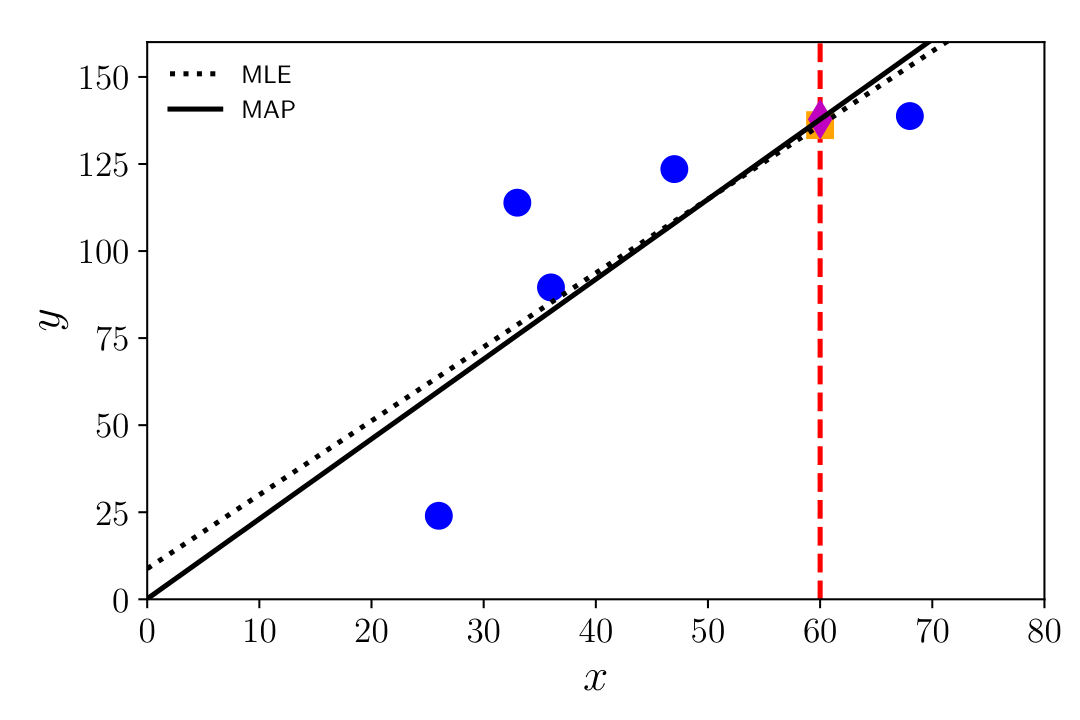
\includegraphics[width=0.92\textwidth,keepaspectratio]{docs/images/Figure8.6.png}
\caption*{\refstepcounter{figcounter}\label{fig:8-6}图~\thefigcounter}
\end{figure}


\subsection*{例 8.6}
\addcontentsline{toc}{subsubsection}{例 8.6}

除前例中的高斯似然假设外，我们假设参数向量服从零均值的多元高斯分布，即 $ p(\boldsymbol{\theta}) = \mathcal{N}(\mathbf{0}, \boldsymbol{\Sigma}) $，其中 $ \boldsymbol{\Sigma} $ 为协方差矩阵（6.5 节）。注意，高斯分布的共轭先验仍然是高斯分布（6.6.1 节），因此我们期望后验分布同样是一个高斯分布。我们将在第 9 章中看到最大后验估计的详细内容。

在机器学习中，纳入关于良好参数所在位置的先验知识的做法非常普遍。正如我们在 8.2.3 节中所见，另一种视角是正则化的思想，它引入了一个附加项以将得到的参数偏置向原点附近。最大后验估计可以被视为连接非概率世界与概率世界的桥梁，因为它明确承认了对先验分布的需求，但最终仍然只产生参数的一个点估计。

\begin{notebox}
\textbf{备注} 极大似然估计 $ \boldsymbol{\theta}_{\text{ML}} $ 具有以下优良性质（Lehmann and Casella, 1998; Efron and Hastie, 2016）：

\begin{itemize}
\item \textbf{渐近一致性（Asymptotic consistency）}：在无限多观测的极限下，MLE 收敛于真实值，外加一个近似正态分布的随机误差。
\item 实现这些性质所需的样本量可能相当大。
\item 误差的方差以 $ 1/N $ 的速度衰减，其中 $ N $ 是数据点的数量。
\item 特别是在“小”数据机制下，极大似然估计可能导致严重的过拟合。
\end{itemize}
\end{notebox}

极大似然估计原理（以及最大后验估计）利用概率建模来推理数据和模型参数中的不确定性。然而，我们尚未将概率建模的潜力发挥到极致。在本节中，最终得到的训练流程仍然产生预测器的点估计，即训练返回一组代表最佳预测器的单一参数值。在 8.4 节中，我们将采取参数值本身也应被视为随机变量的观点，并在做出预测时利用完整的参数分布，而不是估计该分布的“最佳”单个值。

\medskip\hrule\medskip

\section*{8.3.3 模型拟合}
\addcontentsline{toc}{subsection}{8.3.3 模型拟合}

考虑给定一个数据集，我们感兴趣的是将一个参数化模型拟合到该数据集上。当我们谈论“拟合”时，通常是指优化/学习模型参数，使它们最小化某个损失函数，例如负对数似然。通过极大似然（8.3.1 节）和最大后验估计（8.3.2 节），我们已经讨论了两种常用于模型拟合的算法。

模型的参数化定义了一个我们可以据此运作的模型类 $ \mathcal{M}_{\boldsymbol{\theta}} $。例如，在线性回归设定中，我们可以将输入 $ x $ 与（无噪声）观测值 $ y $ 之间的关系定义为 $ y = ax + b $，其中 $ \boldsymbol{\theta} := \{a, b\} $ 为模型参数。在这种情况下，模型参数 $ \boldsymbol{\theta} $ 描述了仿射函数族，即斜率为 $ a $、偏置截距为 $ b $ 的直线族。假设数据来自对我们而言未知的模型 $ \mathcal{M}^* $。对于给定的训练数据集，我们优化 $ \boldsymbol{\theta} $，使 $ \mathcal{M}_{\boldsymbol{\theta}} $ 尽可能接近 $ \mathcal{M}^* $，其中“接近程度”由我们优化的目标函数（例如训练数据上的平方损失）来定义。图~\ref{fig:8-7} 展示了一个场景：我们拥有一个较小的模型类（由圆圈 $ \mathcal{M}_{\boldsymbol{\theta}} $ 表示），而数据生成模型 $ \mathcal{M}^* $ 位于所考虑的模型集之外。我们从 $ \mathcal{M}_{\boldsymbol{\theta}_0} $ 开始参数搜索。在优化之后，即当我们获得最佳可能参数 $ \boldsymbol{\theta}^* $ 时，我们区分三种不同的情况：（i）过拟合；（ii）欠拟合；（iii）拟合良好。我们将给出关于这三个概念的高层直觉。


\begin{figure}[H]
\centering
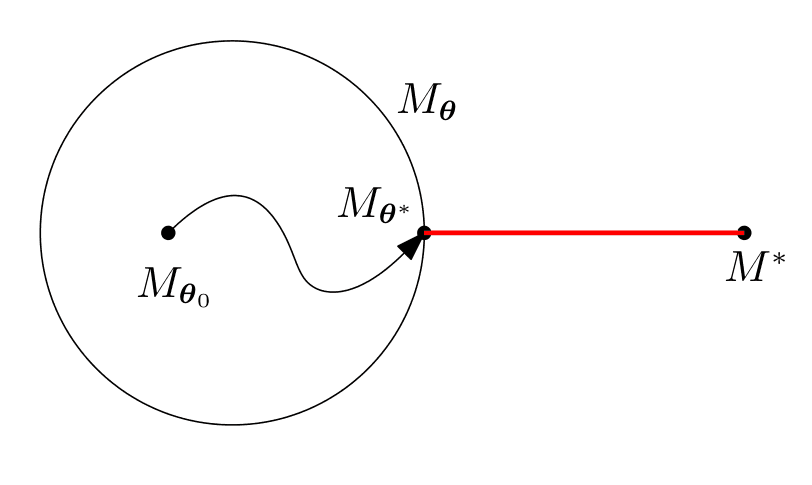
\includegraphics[width=0.92\textwidth,keepaspectratio]{docs/images/Figure8.7.png}
\caption*{\refstepcounter{figcounter}\label{fig:8-7}图~\thefigcounter}
\end{figure}


粗略地说， \emph{过拟合（overfitting）} 是指参数化模型类对于建模由 $ \mathcal{M}^* $ 生成的数据集而言过于丰富，即 $ \mathcal{M}_{\boldsymbol{\theta}} $ 可以建模复杂得多的数据集。例如，如果数据集是由线性函数生成的，而我们将 $ \mathcal{M}_{\boldsymbol{\theta}} $ 定义为七阶多项式类，那么我们不仅可以建模线性函数，还可以建模二次、三次等多项式。过拟合的模型通常具有大量的参数。在实践中检测过拟合的一种方法是在交叉验证期间观察到模型具有较低的训练风险但具有较高的测试风险（8.2.4 节）。我们经常做出的一个观察是，过于灵活的模型类 $ \mathcal{M}_{\boldsymbol{\theta}} $ 会倾尽其所有的建模能力来降低训练误差。因此，如果训练数据存在噪声，它甚至会在噪声本身中寻找某些有用的信号。当我们在远离训练数据的地方进行预测时，这将导致巨大的问题。图~\ref{fig:8-8}(a) 给出了在回归背景下通过极大似然估计学习模型参数时发生过拟合的示例（参见 8.3.1 节）。我们将在 9.2.2 节中进一步讨论回归中的过拟合。

当遇到 \emph{欠拟合（underfitting）} 是指模型类 $ \mathcal{M}_{\boldsymbol{\theta}} $ 不够丰富。例如，如果我们的数据集是由正弦函数生成的，但 $ \boldsymbol{\theta} $ 仅能参数化直线，那么无论多么优秀的优化过程都无法使我们接近真实模型。不过，我们仍然可以优化参数并找到建模该数据集的最佳直线。图~\ref{fig:8-8}(b) 展示了由于灵活性不足而欠拟合的模型示例。欠拟合的模型通常参数很少。

第三种情况是参数化模型类“恰到好处”。此时，我们的模型拟合良好，即它既不过拟合也不欠拟合。这意味着我们的模型类刚好足够丰富以描述所给定的数据集。图~\ref{fig:8-8}(c) 展示了一个与给定数据集拟合得相当好的模型。理想情况下，这正是我们希望使用的模型类，因为它具有良好的泛化性质。


\begin{figure}[H]
\centering
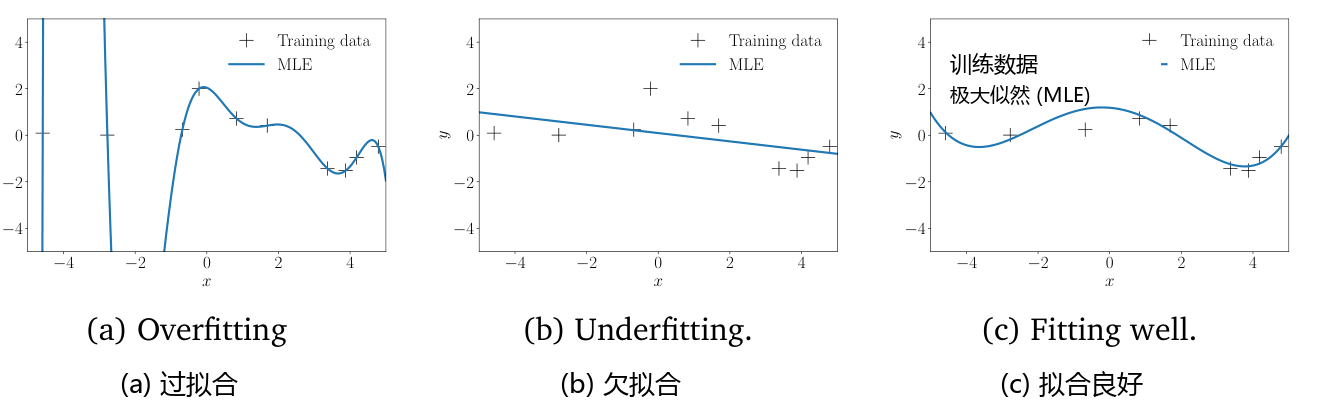
\includegraphics[width=0.92\textwidth,keepaspectratio]{docs/images/Figure8.8.png}
\caption*{\refstepcounter{figcounter}\label{fig:8-8}图~\thefigcounter}
\end{figure}


在实践中，我们经常定义具有海量参数的极其丰富的模型类 $ \mathcal{M}_{\boldsymbol{\theta}} $，例如深度神经网络。为了缓解过拟合问题，我们可以使用正则化（8.2.3 节）或先验（8.3.2 节）。我们将在 8.6 节中讨论如何选择模型类。

\medskip\hrule\medskip

\section*{8.3.4 延伸阅读}
\addcontentsline{toc}{subsection}{8.3.4 延伸阅读}

在考虑概率模型时，极大似然估计原理推广了线性模型的最小二乘回归思想，我们将在第 9 章中对其进行详细讨论。当限制预测器为线性形式并对输出应用额外的非线性函数 $ \phi $ 时，即：

\begin{equation}
p(y_n \mid \boldsymbol{x}_n, \boldsymbol{\theta}) = \phi(\boldsymbol{\theta}^\top \boldsymbol{x}_n)
\tag{8.21}\label{eq:8-21}
\end{equation}

我们可以考虑针对其他预测任务的其他模型，例如二分类或计数数据建模（McCullagh and Nelder, 1989）。对此的另一种视角是考虑来自指数族的似然函数（6.6 节）。这类在参数和数据之间具有线性依赖关系、并具有潜在非线性变换 $ \phi $（称为 \emph{连接函数（link function）}）的模型被称为 \emph{广义线性模型（generalized linear models）} （Agresti, 2002, chapter 4）。

极大似然估计历史悠久，最初由 Ronald Fisher 爵士在 20 世纪 30 年代提出。我们将在 8.4 节进一步扩展概率模型的思想。在使用概率模型的研究人员之间，一个长期的争论是贝叶斯统计与频率学派统计之间的讨论。正如 6.1.1 节所述，这归结为对概率本身的定义。回想 6.1 节，我们可以将概率视为逻辑推理的一种推广（通过允许不确定性）（Cheeseman, 1985; Jaynes, 2003）。极大似然估计方法在本质上属于频率学派，感兴趣的读者可参阅 Efron and Hastie (2016)，以获得对贝叶斯和频率学派统计的客观均衡视角。

对于某些概率模型，极大似然估计可能并不可行。读者可参阅更高级的统计学教材（例如 Casella and Berger, 2002），了解矩估计（method of moments）、M-估计（M-estimation）以及估计方程（estimating equations）等方法。

\section*{8.4 概率建模与推断}
\addcontentsline{toc}{section}{8.4 概率建模与推断}
\label{sec:8.4}

在机器学习中，我们经常关注对数据的解释与分析，例如用于预测未来事件和辅助决策制定。为了使这一任务更易于处理，我们通常会构建描述生成观测数据之 \emph{生成过程（generative process）} 的模型。

例如，我们可以分两步描述掷硬币实验的结果（“正面”或“反面”）。首先，我们定义一个参数 $ \mu $，该参数作为伯努利分布（第 6 章）的参数来描述出现“正面”的概率；其次，我们可以从伯努利分布 $ p(x \mid \mu) = \text{Ber}(\mu) $ 中采样一个结果 $ x \in \{\textcn{正面}, \textcn{反面}\} $。参数 $ \mu $ 产生了一个具体的数据集 $ \mathcal{X} $，并取决于所使用的硬币。由于 $ \mu $ 事先未知且永远无法直接观测，我们需要某种机制在给定掷硬币实验观测结果的情况下来学习关于 $ \mu $ 的知识。接下来，我们将讨论如何利用概率建模来实现这一目的。

\medskip\hrule\medskip

\section*{8.4.1 概率模型}
\addcontentsline{toc}{subsection}{8.4.1 概率模型}

概率模型将实验中不确定的方面表示为概率分布。使用概率模型的优势在于，它们提供了一套来自概率论（第 6 章）的统一且自洽的工具，用于建模、推断、预测和模型选择。概率模型由所有随机变量的联合分布唯一定义。

在概率建模中，观测变量 $ \boldsymbol{x} $ 与隐藏参数 $ \boldsymbol{\theta} $ 的联合分布 $ p(\boldsymbol{x}, \boldsymbol{\theta}) $ 处于核心地位：它囊括了来自以下各个方面的信息：

\begin{enumerate}
\item \textbf{先验与似然}（乘法法则，6.3 节）。
\item \textbf{边缘似然} $ p(\boldsymbol{x}) $（将在 8.6 节的模型选择中扮演重要角色），可以通过对联合分布关于参数进行积分（求和法则，6.3 节）来计算。
\item \textbf{后验分布}，可以通过联合分布除以边缘似然来获得。
\end{enumerate}

唯有联合分布具备这种完备性质。因此，概率模型由其所有随机变量的联合分布来指定。

\medskip\hrule\medskip

\section*{8.4.2 贝叶斯推断}
\addcontentsline{toc}{subsection}{8.4.2 贝叶斯推断}

机器学习的一个核心任务是利用模型和数据，在给定观测变量 $ \boldsymbol{x} $ 的情况下揭示模型隐藏变量 $ \boldsymbol{\theta} $ 的取值。在 8.3.1 节中，我们已经讨论了利用极大似然或最大后验估计来估计模型参数 $ \boldsymbol{\theta} $ 的两种途径。在这两种情形下，我们都获得了 $ \boldsymbol{\theta} $ 的单一最佳值，因此参数估计的核心算法问题即为求解一个优化问题。一旦这些点估计 $ \boldsymbol{\theta}^* $ 已知，我们就使用它们进行预测。更具体地，预测分布将是 $ p(\boldsymbol{x} \mid \boldsymbol{\theta}^*) $，即我们在似然函数中代入 $ \boldsymbol{\theta}^* $。

正如 6.3 节所讨论的，仅仅关注后验分布的某种统计量（例如使后验最大化的参数 $ \boldsymbol{\theta}^* $）会导致信息的丢失，这在依赖预测 $ p(\boldsymbol{x} \mid \boldsymbol{\theta}^*) $ 做出决策的系统中可能是致命的。这些决策系统通常具有与似然不同的目标函数，例如平方误差损失或误分类误差。因此，保留完整的后验分布极具价值，并能带来更具鲁棒性的决策。贝叶斯推断的核心就在于寻找这一后验分布（Gelman et al., 2004）。贝叶斯推断的本质在于学习随机变量的完整分布。对于数据集 $ \mathcal{X} $、参数先验 $ p(\boldsymbol{\theta}) $ 以及似然函数，后验分布：

\begin{equation}
p(\boldsymbol{\theta} \mid \mathcal{X}) = \frac{p(\mathcal{X} \mid \boldsymbol{\theta}) p(\boldsymbol{\theta})}{p(\mathcal{X})}
\tag{8.22}\label{eq:8-22}
\end{equation}

其中：

\begin{equation*}
p(\mathcal{X}) = \int p(\mathcal{X} \mid \boldsymbol{\theta}) p(\boldsymbol{\theta}) d\boldsymbol{\theta}
\end{equation*}

是通过应用贝叶斯定理获得的。其核心思想在于利用贝叶斯定理反转参数 $ \boldsymbol{\theta} $ 与数据 $ \mathcal{X} $ 之间的关系（由似然给出），从而获得后验分布 $ p(\boldsymbol{\theta} \mid \mathcal{X}) $。

拥有参数后验分布的意义在于，它可用于将不确定性从参数传递到数据。更具体地，在参数上具有分布 $ p(\boldsymbol{\theta}) $ 时，我们的预测将为：

\begin{equation}
p(\boldsymbol{x}) = \int p(\boldsymbol{x} \mid \boldsymbol{\theta}) p(\boldsymbol{\theta}) d\boldsymbol{\theta} = \mathbb{E}_{\boldsymbol{\theta}}[p(\boldsymbol{x} \mid \boldsymbol{\theta})]
\tag{8.23}\label{eq:8-23}
\end{equation}

此时预测不再依赖于模型参数 $ \boldsymbol{\theta} $，因为 $ \boldsymbol{\theta} $ 已经被边缘化/积分滤除。式~\eqref{eq:8-23} 表明，预测是对所有合理的参数值 $ \boldsymbol{\theta} $ 进行的平均加权，其中合理性程度由参数分布 $ p(\boldsymbol{\theta}) $ 所决定。

在讨论了 8.3 节的参数估计和此处的贝叶斯推断之后，让我们对比这两种学习方法。通过极大似然或 MAP 估计进行的参数估计产生参数的一致点估计 $ \boldsymbol{\theta}^* $，需要解决的核心计算问题是优化。相比之下，贝叶斯推断产生一个（后验）分布，需要解决的核心计算问题是积分。使用点估计进行预测非常直接，而在贝叶斯框架下进行预测则需要求解另一个积分问题；参见式~\eqref{eq:8-23}。然而，贝叶斯推断为我们提供了一种规范的方法来融合先验知识、考虑辅助信息并引入结构化知识，而所有这些在参数估计的语境下都不容易做到。此外，将参数不确定性传播到预测中，在决策系统的风险评估以及数据高效学习背景下的主动探索中具有非凡的价值（Deisenroth et al., 2015; Kamthe and Deisenroth, 2018）。

尽管贝叶斯推断是用于学习参数和进行预测的数学上严谨规范的框架，但由于我们需要求解复杂的积分问题（参见式~\eqref{eq:8-22} 和 (8.23)），它也带来了一些实际挑战。更具体地说，如果我们没有为参数选择共轭先验（6.6.1 节），式~\eqref{eq:8-22} 和 (8.23) 中的积分在解析上是不可积的，我们将无法以闭式计算后验分布、预测分布或边缘似然。在这些情况下，我们需要求助于近似方法。在这里，我们可以使用随机近似，例如马尔可夫链蒙特卡洛（MCMC）（Gilks et al., 1996），或确定性近似，例如拉普拉斯近似（Laplace approximation）（Bishop, 2006; Barber, 2012; Murphy, 2012）、变分推断（variational inference）（Jordan et al., 1999; Blei et al., 2017）或期望传播（expectation propagation）（Minka, 2001a）。

尽管存在这些挑战，贝叶斯推断已成功应用于各种实际问题，包括大规模主题建模（Hoffman et al., 2013）、点击率预测（Graepel et al., 2010）、控制系统中的数据高效强化学习（Deisenroth et al., 2015）、在线排名系统（Herbrich et al., 2007）以及大规模推荐系统。此外，贝叶斯优化（Brochu et al., 2009; Snoek et al., 2012; Shahriari et al., 2016）等通用工具，对于模型或算法元参数的高效搜索是非常有力的利器。

\begin{notebox}
\textbf{备注} 在机器学习文献中，（随机）“变量”与“参数”之间可能存在某种相对随意的界限划分。通常，参数是被估计出来的（例如通过极大似然），而变量通常是被边缘化积分消除的。在本书中，我们并不严格拘泥于这种划分，因为原则上我们可以为任何参数赋予一个先验并将其积分消除，根据前述划分，这将把该参数转化为随机变量。
\end{notebox}

\medskip\hrule\medskip

\section*{8.4.3 隐变量模型}
\addcontentsline{toc}{subsection}{8.4.3 隐变量模型}

在实践中，将额外的 \emph{隐变量（latent variables）} $ \boldsymbol{z} $（除模型参数 $ \boldsymbol{\theta} $ 之外）作为模型的一部分有时会非常有用（Moustaki et al., 2015）。这些隐变量不同于模型参数 $ \boldsymbol{\theta} $，因为它们不显式地参数化模型。隐变量可以描述数据生成过程，从而有助于提高模型的可解释性。它们还往往能简化模型的结构，使我们能够定义更简单却更丰富的模型架构。模型结构的简化往往与模型参数数量的减少相辅相成（Paquet, 2008; Murphy, 2012）。在隐变量模型中进行学习（至少通过极大似然）可以利用期望最大化（Expectation-Maximization, EM）算法以规范方式完成（Dempster et al., 1977; Bishop, 2006）。引入隐变量有所助益的典型例子包括：用于降维的主成分分析（第 10 章）、用于密度估计的高斯混合模型（第 11 章）、用于时间序列建模的隐马尔可夫模型（Maybeck, 1979）或动力系统（Ghahramani and Roweis, 1999; Ljung, 1999），以及元学习与任务泛化（Hausman et al., 2018; Sæmundsson et al., 2018）。尽管引入隐变量可能使模型结构和生成过程更加清晰，但隐变量模型中的学习通常非常困难，正如我们将在第 11 章中看到的那样。

由于隐变量模型允许我们定义从参数生成数据的过程，让我们仔细考察这个生成过程。用 $ \boldsymbol{x} $ 表示数据，$ \boldsymbol{\theta} $ 表示模型参数，$ \boldsymbol{z} $ 表示隐变量，我们得到条件分布：

\begin{equation}
p(\boldsymbol{x} \mid \boldsymbol{\theta}, \boldsymbol{z})
\tag{8.24}\label{eq:8-24}
\end{equation}

它允许我们针对任何模型参数和隐变量生成数据。鉴于 $ \boldsymbol{z} $ 是隐变量，我们在其上设置先验分布 $ p(\boldsymbol{z}) $。

与我们前面讨论的模型一样，含有隐变量的模型也可以在 8.3 节和 8.4.2 节讨论的框架内用于参数学习和推断。为了便于学习（例如通过极大似然估计或贝叶斯推断），我们遵循两步流程：首先，计算模型的似然 $ p(\boldsymbol{x} \mid \boldsymbol{\theta}) $，它不依赖于隐变量；其次，将该似然用于参数估计或贝叶斯推断，其表达式分别与 8.3 节和 8.4.2 节中的完全一致。由于似然函数 $ p(\boldsymbol{x} \mid \boldsymbol{\theta}) $ 是给定模型参数下数据的预测分布，我们需要将隐变量边缘化消除，从而：

\begin{equation}
p(\boldsymbol{x} \mid \boldsymbol{\theta}) = \int p(\boldsymbol{x} \mid \boldsymbol{\theta}, \boldsymbol{z}) p(\boldsymbol{z}) d\boldsymbol{z}
\tag{8.25}\label{eq:8-25}
\end{equation}

其中 $ p(\boldsymbol{x} \mid \boldsymbol{z}, \boldsymbol{\theta}) $ 由式~\eqref{eq:8-24} 给出，$ p(\boldsymbol{z}) $ 是隐变量上的先验分布。请注意，似然绝不能依赖于隐变量 $ \boldsymbol{z} $，而只能是数据 $ \boldsymbol{x} $ 和模型参数 $ \boldsymbol{\theta} $ 的函数。似然是数据和模型参数的函数，但独立于隐变量。

式~\eqref{eq:8-25} 中的似然直接允许通过极大似然进行参数估计。如 8.3.2 节所讨论的，在对模型参数 $ \boldsymbol{\theta} $ 添加额外先验后，MAP 估计同样是直接明了的。此外，利用似然 (8.25)，隐变量模型中的贝叶斯推断（8.4.2 节）以通常方式运作：我们在模型参数上设置先验 $ p(\boldsymbol{\theta}) $，并利用贝叶斯定理获得在给定数据集 $ \mathcal{X} $ 下模型参数的后验分布：

\begin{equation}
p(\boldsymbol{\theta} \mid \mathcal{X}) = \frac{p(\mathcal{X} \mid \boldsymbol{\theta}) p(\boldsymbol{\theta})}{p(\mathcal{X})} .
\tag{8.26}\label{eq:8-26}
\end{equation}

式~\eqref{eq:8-26} 中的后验分布可用于贝叶斯推断框架下的预测；参见式~\eqref{eq:8-23}。

在隐变量模型中我们面临的一个挑战在于，似然 $ p(\mathcal{X} \mid \boldsymbol{\theta}) $ 需要根据式~\eqref{eq:8-25} 对隐变量进行边缘化。除非我们为 $ p(\boldsymbol{x} \mid \boldsymbol{z}, \boldsymbol{\theta}) $ 选择了共轭先验 $ p(\boldsymbol{z}) $，否则式~\eqref{eq:8-25} 中的边缘化在解析上是不可积的，我们需要借助于近似方法（Bishop, 2006; Paquet, 2008; Murphy, 2012; Moustaki et al., 2015）。

类似于参数后验 (8.26)，我们可以根据下式计算隐变量上的后验分布：

\begin{equation}
p(\boldsymbol{z} \mid \mathcal{X}) = \frac{p(\mathcal{X} \mid \boldsymbol{z}) p(\boldsymbol{z})}{p(\mathcal{X})}
\tag{8.27}\label{eq:8-27}
\end{equation}

其中：

\begin{equation*}
p(\mathcal{X} \mid \boldsymbol{z}) = \int p(\mathcal{X} \mid \boldsymbol{z}, \boldsymbol{\theta}) p(\boldsymbol{\theta}) d\boldsymbol{\theta}
\end{equation*}

这里 $ p(\boldsymbol{z}) $ 是隐变量上的先验，而 $ p(\mathcal{X} \mid \boldsymbol{z}) $ 要求我们对模型参数 $ \boldsymbol{\theta} $ 进行积分滤除。

鉴于解析求解积分的巨大困难，显而易见，在一般情况下同时边缘化消除隐变量和模型参数是不可能的（Bishop, 2006; Murphy, 2012）。一个相对更容易计算的量是隐变量上的后验分布，但条件是以模型参数为条件，即：

\begin{equation}
p(\boldsymbol{z} \mid \mathcal{X}, \boldsymbol{\theta}) = \frac{p(\mathcal{X} \mid \boldsymbol{z}, \boldsymbol{\theta}) p(\boldsymbol{z})}{p(\mathcal{X} \mid \boldsymbol{\theta})}
\tag{8.28}\label{eq:8-28}
\end{equation}

其中 $ p(\boldsymbol{z}) $ 是隐变量上的先验，$ p(\mathcal{X} \mid \boldsymbol{z}, \boldsymbol{\theta}) $ 由式~\eqref{eq:8-24} 给出。

在第 10 章和第 11 章中，我们将分别推导 PCA 和高斯混合模型的似然函数。此外，我们将针对 PCA 和高斯混合模型分别计算隐变量上的条件后验分布 (8.28)。

\begin{notebox}
\textbf{备注} 在接下来的章节中，我们可能不会对隐变量 $ \boldsymbol{z} $ 与不确定的模型参数 $ \boldsymbol{\theta} $ 做出如此清晰的区分，因为它们都是未被直接观测到的，有时会统称为“潜变量”或“隐藏变量”。在第 10 章和第 11 章中，由于同时存在模型参数 $ \boldsymbol{\theta} $ 和隐变量 $ \boldsymbol{z} $ 这两类不同的隐藏变量，我们将格外关注它们之间的区别。
\end{notebox}

我们可以利用概率模型的所有元素都是随机变量这一事实，定义一种统一的语言来表示它们。在 8.5 节中，我们将看到一种用于表示概率模型结构的简洁图语言。我们将在随后的章节中利用这种图语言来描述各种概率模型。

\medskip\hrule\medskip

\section*{8.4.4 延伸阅读}
\addcontentsline{toc}{subsection}{8.4.4 延伸阅读}

机器学习中的概率模型（Bishop, 2006; Barber, 2012; Murphy, 2012）为使用者以规范的方式捕捉关于数据和预测模型的不确定性提供了途径。Ghahramani (2015) 简要综述了机器学习中的概率模型。给定一个概率模型，我们或许有幸能够解析地计算出感兴趣的参数。然而在一般情况下，解析解非常罕见，通常会使用采样（Gilks et al., 1996; Brooks et al., 2011）和变分推断（Jordan et al., 1999; Blei et al., 2017）等计算方法。Moustaki et al. (2015) 和 Paquet (2008) 对隐变量模型中的贝叶斯推断提供了优良的概述。

近年来，学术界提出了若干旨在将软件中定义的变量视为对应于概率分布之随机变量的编程语言。其目标是使用户能够编写概率分布的复杂函数，而底层编译器会自动处理贝叶斯推断的各项法则。这一快速发展的领域被称为 \emph{概率编程（probabilistic programming）} 。

\section*{8.5 有向图模型}
\addcontentsline{toc}{section}{8.5 有向图模型}
\label{sec:8.5}

在本节中，我们介绍一种用于指定概率模型的图语言，称为 \emph{有向图模型（directed graphical model）} 。它提供了一种紧凑且简洁的方式来定义概率模型，并允许读者直观地解析随机变量之间的依赖关系。图模型直观地捕捉了所有随机变量上的联合分布如何分解为仅依赖于这些变量子集的因子乘积。在 8.4 节中，我们将概率模型的联合分布确定为核心关注量，因为它包含了关于先验、似然和后验的全部信息。然而，联合分布本身可能极其复杂，并且它无法直接向我们揭示概率模型的结构性质。例如，联合分布 $ p(a, b, c) $ 本身并不能直观告诉我们变量之间的任何独立性关系。这正是图模型发挥作用之处。本节依赖于 6.4.5 节中描述的独立性与条件独立性概念。

在图模型中，节点代表随机变量。在图~\ref{fig:8-9}(a) 中，节点分别表示随机变量 $ a, b, c $。边代表变量之间的概率关系，例如条件概率。有向图模型也被称为 \emph{贝叶斯网络（Bayesian networks）} 。

\begin{notebox}
\textbf{备注} 并非任何分布都可以由特定选取的图模型精确表示。对此的深入讨论可参见 Bishop (2006)。
\end{notebox}

概率图模型具有许多极为便利的性质：

\begin{itemize}
\item 它们提供了一种直观可视化概率模型结构的简单方式。
\item 它们可用于设计或启发新型统计模型。
\item 仅通过检查图的拓扑结构，就能深入洞察模型的代数性质，例如条件独立性。
\item 统计模型中用于推断和学习的复杂计算，可以通过图上的局部操作（消息传递）直观表达。
\end{itemize}

\medskip\hrule\medskip

\section*{8.5.1 图语义}
\addcontentsline{toc}{subsection}{8.5.1 图语义}

有向图模型（贝叶斯网络）是一种表示概率模型中条件依赖关系的方法。它们提供了条件概率的可视化描述，从而为描述复杂的相互依赖关系提供了一种简单的语言。在附加假设下，有向箭头还可用于表示因果关系（Pearl, 2009）。这种模块化描述还带来了计算上的大幅简化。两个节点（随机变量）之间的有向连接（箭头）表示条件概率。例如，图~\ref{fig:8-9}(a) 中 $ a $ 和 $ b $ 之间的箭头表示给定 $ a $ 时 $ b $ 的条件概率 $ p(b \mid a) $。


\begin{figure}[H]
\centering
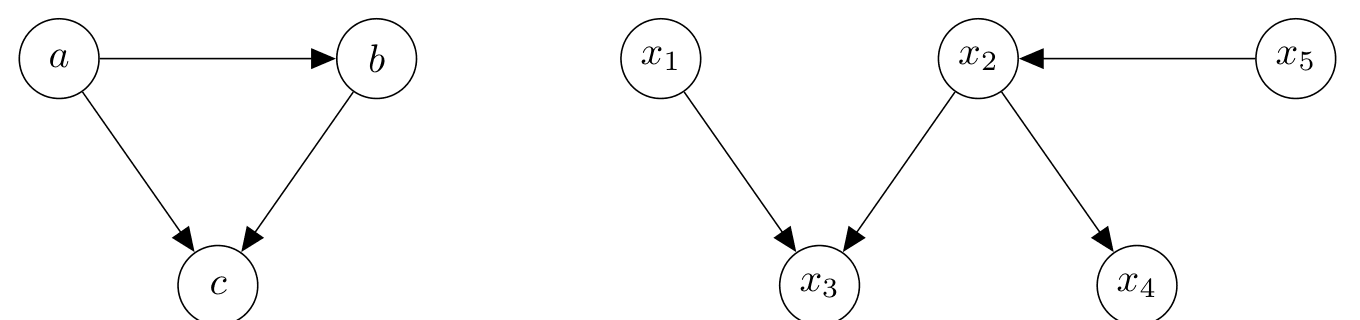
\includegraphics[width=0.92\textwidth,keepaspectratio]{docs/images/Figure8.9.png}
\caption*{\refstepcounter{figcounter}\label{fig:8-9}图~\thefigcounter}
\end{figure}


如果我们了解联合分布因式分解的某些性质，就可以直接从联合分布推导出对应的有向图模型。

\subsection*{例 8.7}
\addcontentsline{toc}{subsubsection}{例 8.7}

考虑三个随机变量 $ a, b, c $ 的联合分布：

\begin{equation}
p(a, b, c) = p(c \mid a, b) p(b \mid a) p(a) .
\tag{8.29}\label{eq:8-29}
\end{equation}

式~\eqref{eq:8-29} 中联合分布的因式分解向我们揭示了随机变量之间的层级关系：

\begin{itemize}
\item $ c $ 直接依赖于 $ a $ 和 $ b $。
\item $ b $ 直接依赖于 $ a $。
\item $ a $ 既不依赖于 $ b $，也不依赖于 $ c $。
\end{itemize}

对于式~\eqref{eq:8-29} 的因式分解，我们得到图~\ref{fig:8-9}(a) 所示的有向图模型。

一般而言，我们可以按照如下步骤从因式分解的联合分布构建对应的有向图模型：

\begin{enumerate}
\item 为所有随机变量分别创建一个节点。
\item 对于每个条件分布，从其所依据的条件变量所对应的节点出发，向该条件分布对应的变量节点添加一条有向边（箭头）。
\end{enumerate}

图的布局结构取决于联合分布因式分解的具体方式。

我们讨论了如何从已知的联合分布因式分解得到对应的有向图模型。现在，我们执行完全相反的操作：描述如何从给定的图模型中提取一组随机变量的联合分布。

\subsection*{例 8.8}
\addcontentsline{toc}{subsubsection}{例 8.8}

考察图~\ref{fig:8-9}(b) 所示的图模型，我们利用两条基本性质：

\begin{enumerate}
\item 我们寻求的联合分布 $ p(x_1, \ldots, x_5) $ 是图中每个节点对应条件分布的乘积。在这个特定示例中，我们需要五个条件分布。
\item 每个条件分布仅依赖于图中对应节点的 \emph{父节点（parents）} 。例如，$ x_4 $ 的条件仅取决于 $ x_2 $。
\end{enumerate}

这两条性质给出了联合分布所需的因式分解：

\begin{equation}
p(x_1, x_2, x_3, x_4, x_5) = p(x_1) p(x_5) p(x_2 \mid x_5) p(x_3 \mid x_1, x_2) p(x_4 \mid x_2) .
\tag{8.30}\label{eq:8-30}
\end{equation}

一般而言，联合分布 $ p(\boldsymbol{x}) = p(x_1, \ldots, x_K) $ 由下式给出：

\begin{equation}
p(\boldsymbol{x}) = \prod_{k=1}^K p\left(x_k \mid \text{Pa}_k\right)
\tag{8.31}\label{eq:8-31}
\end{equation}

其中 $ \text{Pa}_k $ 表示“$ x_k $ 的父节点集合”。$ x_k $ 的父节点是指有箭头直接指向 $ x_k $ 的所有节点。

我们以抛硬币实验的具体示例来结束本小节。考虑一个伯努利实验（例 6.8），其中该实验结果 $ x $ 为“正面”的概率为：

\begin{equation}
p(x \mid \mu) = \text{Ber}(\mu) .
\tag{8.32}\label{eq:8-32}
\end{equation}

我们现在将该实验重复 $ N $ 次并观测到结果 $ x_1, \ldots, x_N $，从而获得联合分布：

\begin{equation}
p(x_1, \ldots, x_N \mid \mu) = \prod_{n=1}^N p(x_n \mid \mu) .
\tag{8.33}\label{eq:8-33}
\end{equation}

右侧的表达式是每个单独结果的伯努利分布的乘积，因为每次实验是独立的。回想 6.4.5 节，统计独立性意味着分布可以因式分解。为了写出该设定的图模型，我们对未观测/隐变量与已观测变量进行区分。在图示中，已观测变量由阴影节点表示，从而得到图~\ref{fig:8-10}(a) 中的图模型。我们看到，由于结果 $ x_n $ 是同分布的，单一参数 $ \mu $ 对所有 $ x_n $（$ n = 1, \ldots, N $）都是相同的。针对该设定的一种更紧凑但完全等价的图模型如图~\ref{fig:8-10}(b) 所示，其中我们使用了 \emph{板块表示法（plate notation）} 。板块（矩形框）将内部的所有内容（在此例中为观测值 $ x_n $）重复 $ N $ 次。因此，这两个图模型是等价的，但板块表示法紧凑得多。


\begin{figure}[H]
\centering
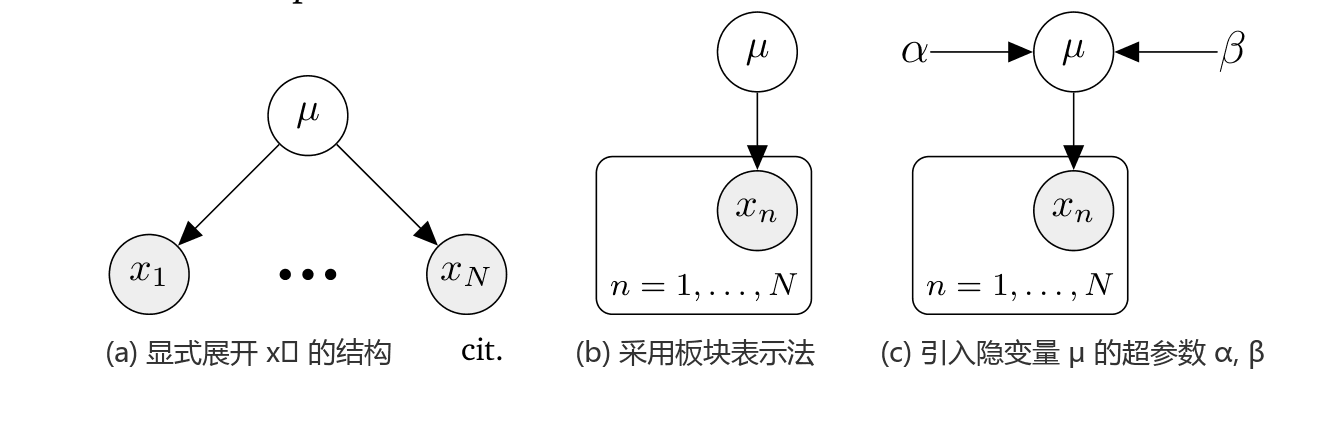
\includegraphics[width=0.92\textwidth,keepaspectratio]{docs/images/Figure8.10.png}
\caption*{\refstepcounter{figcounter}\label{fig:8-10}图~\thefigcounter}
\end{figure}


图模型允许我们直接在 $ \mu $ 上设置 \emph{超先验（hyperprior）} 。超先验是针对第一层先验参数设立的第二层先验分布。图~\ref{fig:8-10}(c) 在隐变量 $ \mu $ 上引入了 $ \text{Beta}(\alpha, \beta) $ 先验。如果我们将 $ \alpha $ 和 $ \beta $ 视为确定性参数（即非随机变量），我们通常省略其外侧的圆圈。

\medskip\hrule\medskip

\section*{8.5.2 条件独立性与 d-分离}
\addcontentsline{toc}{subsection}{8.5.2 条件独立性与 d-分离}

有向图模型允许我们仅仅通过观察图的拓扑结构来确定联合分布的条件独立性（6.4.5 节）性质。被称为 \emph{d-分离（d-separation）} （Pearl, 1988）的概念是这一分析的关键。

考虑一个一般的有向图，其中 $ A, B, C $ 是互不相交的任意节点子集（它们的并集可以小于图中节点的完整集合）。我们希望确定给定的有向无环图是否蕴含特定的条件独立性陈述：“在给定 $ C $ 的条件下，$ A $ 与 $ B $ 条件独立”，记作：

\begin{equation}
A \perp\perp B \mid C .
\tag{8.34}\label{eq:8-34}
\end{equation}

为此，我们考虑从集合 $ A $ 中的任意节点到集合 $ B $ 中的任意节点的所有可能无向轨迹（忽略箭头方向的路径）。如果任何此类路径包含满足以下任一条件的节点，则称该路径被 \emph{阻断（blocked）} ：

\begin{enumerate}
\item 路径上的箭头在该节点处相遇形式为“头对尾”（head-to-tail）或“尾对尾”（tail-to-tail），并且该节点位于集合 $ C $ 中。
\item 路径上的箭头在该节点处相遇形式为“头对头”（head-to-head），并且该节点及其所有后代节点均不在集合 $ C $ 中。
\end{enumerate}

如果连接 $ A $ 与 $ B $ 的所有可能路径都被阻断，则称集合 $ A $ 在给定 $ C $ 的条件下与集合 $ B $ 实现了 \emph{d-分离（d-separation）} ，并且图中所有变量上的联合分布都将严格满足 $ A \perp\perp B \mid C $。


\begin{figure}[H]
\centering
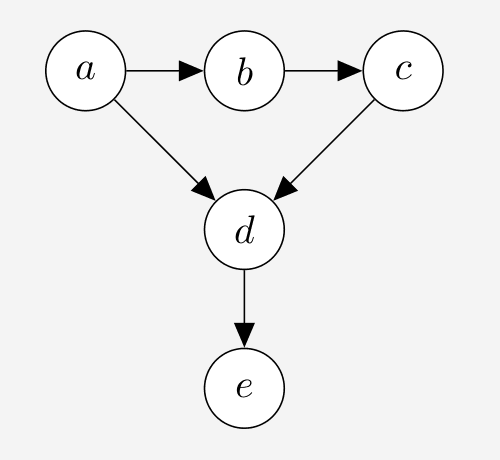
\includegraphics[width=0.92\textwidth,keepaspectratio]{docs/images/Figure8.11.png}
\caption*{\refstepcounter{figcounter}\label{fig:8-11}图~\thefigcounter}
\end{figure}


\subsection*{例 8.9（条件独立性）}
\addcontentsline{toc}{subsubsection}{例 8.9（条件独立性）}

考虑图~\ref{fig:8-11} 所示的图模型。直观检查拓扑结构可得：

\begin{equation}
b \perp\perp d \mid a, c
\tag{8.35}\label{eq:8-35}
\end{equation}

\begin{equation}
a \perp\perp c \mid b
\tag{8.36}\label{eq:8-36}
\end{equation}

\begin{equation}
b \not\perp\perp d \mid c
\tag{8.37}\label{eq:8-37}
\end{equation}

\begin{equation}
a \not\perp\perp c \mid b, e
\tag{8.38}\label{eq:8-38}
\end{equation}

有向图模型允许对概率模型进行高度紧凑的表示，我们将在第 9、10 和 11 章中看到有向图模型的广泛应用。该表示形式结合条件独立性概念，使我们能够将各自的概率模型因式分解为更易于优化的局部表达式。

概率模型的图表示使我们能够直观地看到我们在模型结构上所做出的设计选择的影响。我们经常需要对模型的结构做出高层次的假设。这些建模假设（超参数）会影响预测性能，但无法直接使用我们目前所看到的方法进行选取。我们将在 8.6 节中讨论选择模型结构的不同方法。

\medskip\hrule\medskip

\section*{8.5.3 延伸阅读}
\addcontentsline{toc}{subsection}{8.5.3 延伸阅读}

关于概率图模型的导论可参阅 Bishop (2006, 第 8 章)，关于各种应用及相应算法影响的详尽阐述可参阅 Koller and Friedman (2009) 的经典著作。概率图模型主要有三种基本类型：

\begin{enumerate}
\item \textbf{有向图模型（贝叶斯网络）}；参见图~\ref{fig:8-12}(a)。
\item \textbf{无向图模型（马尔可夫随机场）}；参见图~\ref{fig:8-12}(b)。
\item \textbf{因子图（Factor graphs）}；参见图~\ref{fig:8-12}(c)。
\end{enumerate}


\begin{figure}[H]
\centering
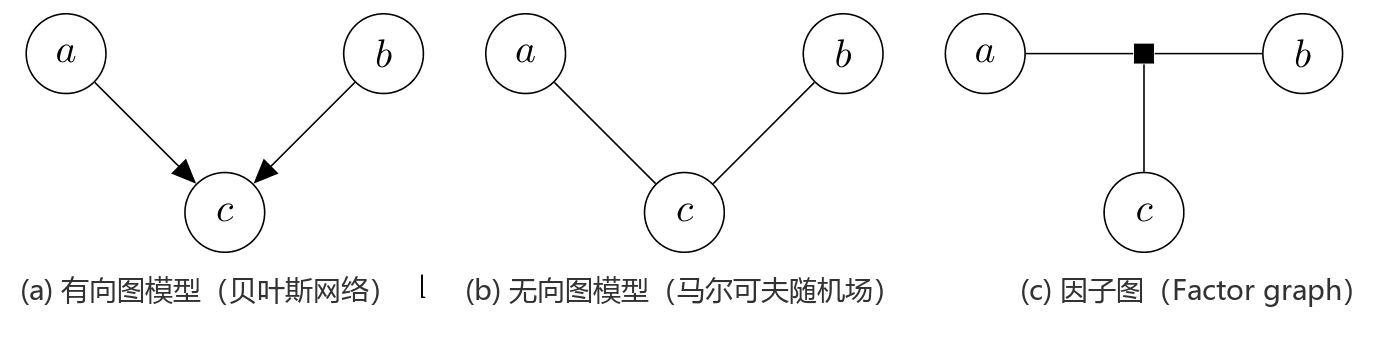
\includegraphics[width=0.92\textwidth,keepaspectratio]{docs/images/Figure8.12.png}
\caption*{\refstepcounter{figcounter}\label{fig:8-12}图~\thefigcounter}
\end{figure}


图模型允许利用基于图的算法进行推断和学习，例如通过局部消息传递（local message passing）。其应用范围涵盖在线游戏排位（Herbrich et al., 2007）、计算机视觉（例如图像分割、语义标注、图像去噪、图像复原（Kittler and Föglein, 1984; Sucar and Gillies, 1994; Shotton et al., 2006; Szeliski et al., 2008））、编码理论（McEliece et al., 1998）、线性方程组求解（Shental et al., 2008）以及信号处理中的迭代贝叶斯状态估计（Bickson et al., 2007; Deisenroth and Mohamed, 2012）。

在实际应用中极其重要但在本书中未深入探讨的一个主题是 \emph{结构化预测（structured prediction）} （Bakir et al., 2007; Nowozin et al., 2014），它使机器学习模型能够处理序列、树和图等具有内部结构的预测任务。神经网络模型的普及催生了更灵活的概率模型，产生了结构化模型的诸多成功应用（Goodfellow et al., 2016, 第 16 章）。近年来，由于图模型在因果推断中的重要应用，人们对图模型重新燃起了浓厚兴趣（Pearl, 2009; Imbens and Rubin, 2015; Peters et al., 2017; Rosenbaum, 2017）。

\section*{8.6 模型选择}
\addcontentsline{toc}{section}{8.6 模型选择}
\label{sec:8.6}

在机器学习中，我们经常需要做出对模型性能产生决定性影响的高层次建模决策。我们所做的选择（例如似然函数的函数形式）直接影响模型中自由参数的数量和类型，从而也决定了模型的灵活性与表达能力。更复杂的模型在能够描述更多数据集的意义上更为灵活。例如，1 次多项式（直线 $ y = a_0 + a_1 x $）只能用于描述输入 $ x $ 与观测值 $ y $ 之间的线性关系。而 2 次多项式（$ y = a_0 + a_1 x + a_2 x^2 $）通过令 $ a_2 = 0 $ 也可以描述线性函数，即它在表达能力上严格强于 1 次多项式，并且能够额外描述输入与观测值之间的二次曲线关系。

人们可能会认为，非常灵活的模型由于表达能力更强，因而通常比简单模型更具优势。然而，一个普遍的问题在于，在训练阶段我们只能使用训练集来评估模型的性能并学习其参数。但我们在训练集上的表现并非我们真正关注的目标。在 8.3 节中，我们已经看到极大似然估计可能导致严重的过拟合，特别是在训练数据集较小的情况下。在理想情况下，我们的模型（也）应当在测试集（在训练时不可见）上表现良好。因此，我们需要某种机制来评估模型如何泛化到未见过的测试数据。 \emph{模型选择（model selection）} 所关注的正是这个问题。

\medskip\hrule\medskip

\section*{8.6.1 嵌套交叉验证}
\addcontentsline{toc}{subsection}{8.6.1 嵌套交叉验证}

我们已经见识过一种可用于模型选择的方法（8.2.4 节中的交叉验证）。回想一下，交叉验证通过重复将数据集划分为训练集和验证集来提供泛化误差的估计。我们可以将这一思想再次应用，即对于每次划分，我们再执行另一轮交叉验证。这被称为 \emph{嵌套交叉验证（nested cross-validation）} ；参见图~\ref{fig:8-13}。


\begin{figure}[H]
\centering
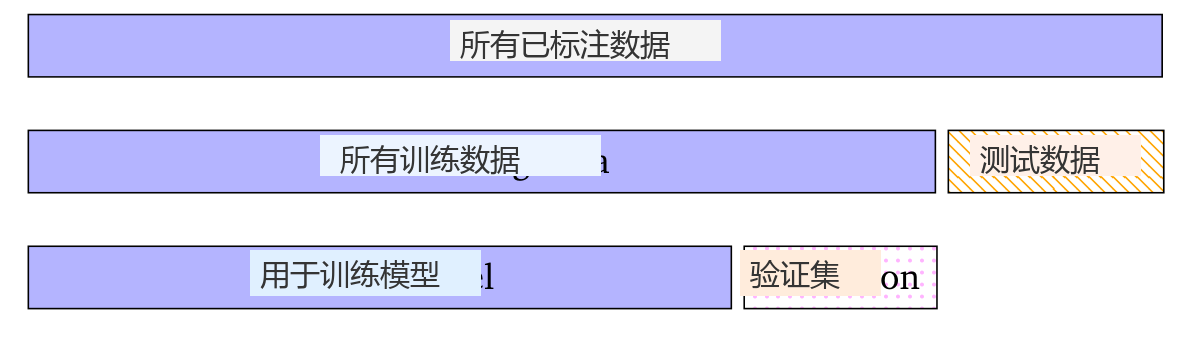
\includegraphics[width=0.92\textwidth,keepaspectratio]{docs/images/Figure8.13.png}
\caption*{\refstepcounter{figcounter}\label{fig:8-13}图~\thefigcounter}
\end{figure}


内层循环用于在内部验证集上评估特定模型或超参数选择的性能。外层循环用于评估由内层循环挑选出的最佳模型的泛化性能。我们可以在内层循环中测试不同的模型和超参数选择。为了区分这两个层级，通常将用于估计泛化性能的集合称为 \emph{测试集（test set）} ，而将用于选择最佳模型的集合称为 \emph{验证集（validation set）} 。内层循环通过使用验证集上的经验误差进行近似，来估计给定模型的泛化误差期望值：

\begin{equation}
\mathbb{E}_{\mathcal{V}}[R(\mathcal{V} \mid \mathcal{M})] \approx \frac{1}{K} \sum_{k=1}^K R(\mathcal{V}^{(k)} \mid \mathcal{M})
\tag{8.39}\label{eq:8-39}
\end{equation}

其中 $ R(\mathcal{V} \mid \mathcal{M}) $ 是模型 $ \mathcal{M} $ 在验证集 $ \mathcal{V} $ 上的经验风险（例如均方根误差 RMSE）。标准误差定义为 $ \sigma / \sqrt{K} $，其中 $ K $ 是实验次数，$ \sigma $ 是每次实验风险的标准差。我们对所有备选模型重复此过程，并选择表现最佳的模型。请注意，交叉验证不仅为我们提供了期望泛化误差，我们还可以获得更高阶的统计量（例如标准误差），即均值估计不确定性的度量。一旦确定了最终模型，我们就可以在保留的测试集上评估最终的泛化性能。

\medskip\hrule\medskip

\section*{8.6.2 贝叶斯模型选择}
\addcontentsline{toc}{subsection}{8.6.2 贝叶斯模型选择}

模型选择有许多方法，本节将介绍其中一部分。通常，它们都试图在模型复杂度与数据拟合程度之间进行权衡。我们假设简单模型比复杂模型更不容易发生过拟合，因此模型选择的目标是寻找能够合理解释数据的最简单模型。这一概念被称为 \emph{奥卡姆剃刀（Occam's razor）} 。

\begin{notebox}
\textbf{备注} 如果我们将模型选择视为假设检验问题，我们寻求的是与数据一致的最简单假设（Murphy, 2012）。
\end{notebox}

人们可能会考虑在模型上设置一个偏好较简单模型的先验。然而，这样做并非必须：在贝叶斯概率的应用中，已经从数量上自然蕴含了“自动奥卡姆剃刀”（automatic Occam's razor）（Smith and Spiegelhalter, 1980; Jefferys and Berger, 1992; MacKay, 1992）。图~\ref{fig:8-14}（改编自 MacKay, 2003）给出了为什么复杂且高表达力的模型对建模给定数据集 $ \mathcal{D} $ 而言反而可能是概率较低之选择的基本直觉。


\begin{figure}[H]
\centering
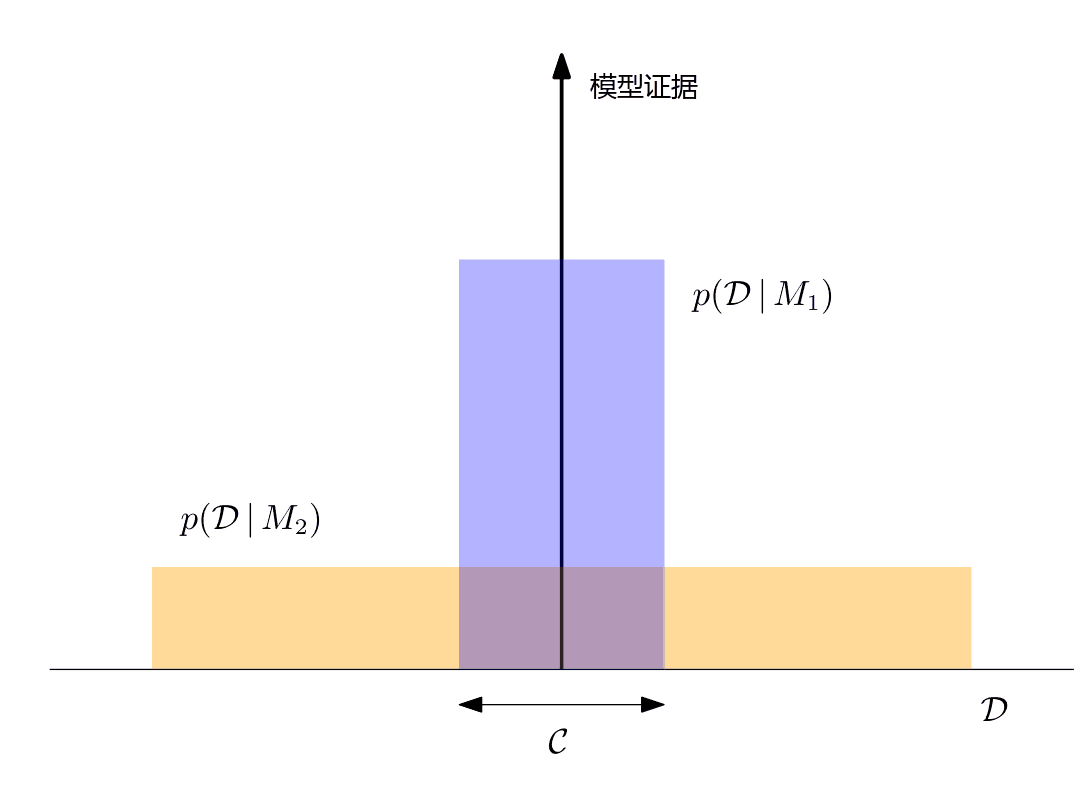
\includegraphics[width=0.92\textwidth,keepaspectratio]{docs/images/Figure8.14.png}
\caption*{\refstepcounter{figcounter}\label{fig:8-14}图~\thefigcounter}
\end{figure}


让我们将横轴想象为所有可能数据集 $ \mathcal{D} $ 的空间。如果我们感兴趣的是在给定数据 $ \mathcal{D} $ 的条件下模型 $ \mathcal{M}_i $ 的后验概率 $ p(\mathcal{M}_i \mid \mathcal{D}) $，我们可以应用贝叶斯定理。假设在所有模型上具有均匀先验 $ p(\mathcal{M}) $，贝叶斯定理按照模型预测实际发生数据的能力成比例地奖励模型。给定模型 $ \mathcal{M}_i $ 时数据的这种预测概率 $ p(\mathcal{D} \mid \mathcal{M}_i) $ 被称为 $ \mathcal{M}_i $ 的 \emph{模型证据（evidence）} 。简单模型 $ \mathcal{M}_1 $ 只能预测一小部分数据集，如 $ p(\mathcal{D} \mid \mathcal{M}_1) $ 所示；而具有更多自由参数的更强大模型 $ \mathcal{M}_2 $ 能够预测种类更多样的数据集。这些预测由 $ \mathcal{D} $ 上的归一化概率分布量化，即对所有可能数据积分或求和必须等于 1。这意味着，$ \mathcal{M}_2 $ 对区域 $ C $ 内的数据集的预测能力不如 $ \mathcal{M}_1 $ 集中。假设为这两个模型分配了相等的先验概率，那么如果数据集落在区域 $ C $ 内，表达能力较弱的模型 $ \mathcal{M}_1 $ 反而是后验概率更高的模型。

在本章早些时候，我们指出模型需要能够解释数据，即应当存在从给定模型生成数据的方法。此外，如果模型已经从数据中进行了适度学习，那么我们期望生成的数据应当与经验观测数据相似。为此，将模型选择表述为分层推断问题是很有帮助的，这使我们能够计算模型集合上的后验分布。

考虑有限个模型构成的集合 $ \mathcal{M} = \{\mathcal{M}_1, \ldots, \mathcal{M}_K\} $，其中每个模型 $ \mathcal{M}_k $ 具有参数 $ \boldsymbol{\theta}_k $。在贝叶斯模型选择中，我们在模型集合上引入先验分布 $ p(\mathcal{M}) $。允许我们从该模型生成数据的对应生成过程为：

\begin{equation}
\mathcal{M}_k \sim p(\mathcal{M})
\tag{8.40}\label{eq:8-40}
\end{equation}

\begin{equation}
\boldsymbol{\theta}_k \sim p(\boldsymbol{\theta} \mid \mathcal{M}_k)
\tag{8.41}\label{eq:8-41}
\end{equation}

\begin{equation}
\mathcal{D} \sim p(\mathcal{D} \mid \boldsymbol{\theta}_k)
\tag{8.42}\label{eq:8-42}
\end{equation}

该层级生成过程如图~\ref{fig:8-15} 所示。


\begin{figure}[H]
\centering
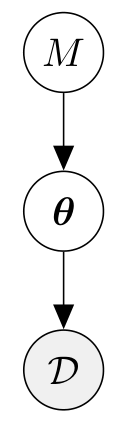
\includegraphics[width=0.41\textwidth,height=0.80\textheight,keepaspectratio]{docs/images/Figure8.15.png}
\caption*{\refstepcounter{figcounter}\label{fig:8-15}图~\thefigcounter}
\end{figure}


给定训练集 $ \mathcal{D} $，我们应用贝叶斯定理并计算模型上的后验分布：

\begin{equation}
p(\mathcal{M}_k \mid \mathcal{D}) \propto p(\mathcal{M}_k) p(\mathcal{D} \mid \mathcal{M}_k) .
\tag{8.43}\label{eq:8-43}
\end{equation}

请注意，该后验不再依赖于模型参数 $ \boldsymbol{\theta}_k $，因为在贝叶斯框架下参数已被积分消除：

\begin{equation}
p(\mathcal{D} \mid \mathcal{M}_k) = \int p(\mathcal{D} \mid \boldsymbol{\theta}_k) p(\boldsymbol{\theta}_k \mid \mathcal{M}_k) d\boldsymbol{\theta}_k
\tag{8.44}\label{eq:8-44}
\end{equation}

其中 $ p(\boldsymbol{\theta}_k \mid \mathcal{M}_k) $ 是模型 $ \mathcal{M}_k $ 的模型参数 $ \boldsymbol{\theta}_k $ 的先验分布。式~\eqref{eq:8-44} 被称为 \emph{模型证据（model evidence）} 或 \emph{边缘似然（marginal likelihood）} 。根据式~\eqref{eq:8-43} 中的后验分布，我们确定 MAP 估计：

\begin{equation}
\mathcal{M}^* = \arg\max_{\mathcal{M}_k} p(\mathcal{M}_k \mid \mathcal{D}) .
\tag{8.45}\label{eq:8-45}
\end{equation}

若采用均匀先验 $ p(\mathcal{M}_k) = \frac{1}{K} $（赋予每个模型相等的先验概率），在模型上确定 MAP 估计等价于选取最大化模型证据 (8.44) 的模型。

\begin{notebox}
\textbf{备注（似然与边缘似然）} 似然与边缘似然（模型证据）之间存在一些重要差异：虽然似然容易出现过拟合，但边缘似然通常不会，因为模型参数已经被边缘化积分消除（即我们不再需要拟合参数）。此外，边缘似然自动体现了模型复杂度与数据拟合之间的权衡（奥卡姆剃刀）。
\end{notebox}

\medskip\hrule\medskip

\section*{8.6.3 用于模型比较的贝叶斯因子}
\addcontentsline{toc}{subsection}{8.6.3 用于模型比较的贝叶斯因子}

考虑在给定数据集 $ \mathcal{D} $ 的情况下比较两个概率模型 $ \mathcal{M}_1, \mathcal{M}_2 $ 的问题。如果我们计算后验概率 $ p(\mathcal{M}_1 \mid \mathcal{D}) $ 和 $ p(\mathcal{M}_2 \mid \mathcal{D}) $，我们可以计算后验概率之比：

\begin{equation}
\begin{adjustbox}{max width=\linewidth}
\underbrace{\frac{p(\mathcal{M}_1 \mid \mathcal{D})}{p(\mathcal{M}_2 \mid \mathcal{D})}}_{\textcn{后验几率}} = \frac{\frac{p(\mathcal{D} \mid \mathcal{M}_1) p(\mathcal{M}_1)}{p(\mathcal{D})}}{\frac{p(\mathcal{D} \mid \mathcal{M}_2) p(\mathcal{M}_2)}{p(\mathcal{D})}} = \underbrace{\frac{p(\mathcal{M}_1)}{p(\mathcal{M}_2)}}_{\textcn{先验几率}} \underbrace{\frac{p(\mathcal{D} \mid \mathcal{M}_1)}{p(\mathcal{D} \mid \mathcal{M}_2)}}_{\textcn{贝叶斯因子}} .
\end{adjustbox}
\tag{8.46}\label{eq:8-46}
\end{equation}

后验的比值被称为 \emph{后验几率（posterior odds）} 。式~\eqref{eq:8-46} 等号右侧的第一个分式为 \emph{先验几率（prior odds）} ，度量了我们的先验信念在多大程度上偏向 $ \mathcal{M}_1 $ 胜过 $ \mathcal{M}_2 $。边缘似然的比值（右侧第二个分式）被称为 \emph{贝叶斯因子（Bayes factor）} ，度量了与 $ \mathcal{M}_2 $ 相比，模型 $ \mathcal{M}_1 $ 预测数据 $ \mathcal{D} $ 的优良程度。

\begin{notebox}
\textbf{备注} \emph{杰弗里斯-林德利悖论（Jeffreys-Lindley paradox）} 指出，“贝叶斯因子总是偏向于更简单的模型，因为在具有弥散先验的复杂模型下，数据的边缘概率将非常小”（Murphy, 2012）。这里的“弥散先验”（diffuse prior）是指不偏向任何特定模型的先验，即在该先验下许多模型在先验上都是合理的。
\end{notebox}

如果我们选择模型上的均匀先验，式~\eqref{eq:8-46} 中的先验几率项为 1，即后验几率等于边缘似然之比（贝叶斯因子）：

\begin{equation}
\frac{p(\mathcal{D} \mid \mathcal{M}_1)}{p(\mathcal{D} \mid \mathcal{M}_2)} .
\tag{8.47}\label{eq:8-47}
\end{equation}

如果贝叶斯因子大于 1，我们选择模型 $ \mathcal{M}_1 $；否则选择模型 $ \mathcal{M}_2 $。与频率学派统计类似，在认定结果具有“统计显著性”之前，对于该比值的大小存在一些参考指南（Jeffreys, 1961）。

\begin{notebox}
\textbf{备注（计算边缘似然）} 边缘似然在模型选择中发挥着核心作用：我们需要计算贝叶斯因子 (8.46) 以及模型上的后验分布 (8.43)。 遗憾的是，计算边缘似然需要我们求解积分 (8.44)。该积分在通常情况下解析不可积，我们将不得不求助于近似技术，例如数值积分（Stoer and Burlirsch, 2002）、利用蒙特卡洛的随机近似（Murphy, 2012）或贝叶斯蒙特卡洛技术（O'Hagan, 1991; Rasmussen and Ghahramani, 2003）。 然而，存在一些可以精确求解的特例。在 6.6.1 节中，我们讨论了共轭模型。如果我们选择共轭参数先验 $ p(\boldsymbol{\theta}) $，我们就可以闭式计算边缘似然。在第 9 章中，我们将在正规线性回归的背景下严格实现这一点。
\end{notebox}

在本章中，我们简要介绍了机器学习的基本概念。在本书第二部分的其余章节中，我们将看到 8.2 节、8.3 节和 8.4 节中的三种不同学习风格如何全面应用于机器学习的四大支柱（回归、降维、密度估计和分类）。

\medskip\hrule\medskip

\section*{8.6.4 延伸阅读}
\addcontentsline{toc}{subsection}{8.6.4 延伸阅读}

我们在本节开头提到，存在影响模型性能的高层建模决策。典型的选择包括：

\begin{itemize}
\item 回归设定中多项式的阶数
\item 混合模型中成分的数量
\item （深度）神经网络的网络架构
\item 支持向量机中核函数的类型
\item PCA 中潜空间的维度
\item 优化算法中的学习率（及衰减计划）
\end{itemize}

在参数模型中，参数数量通常与模型类的复杂度直接相关。Rasmussen and Ghahramani (2001) 指出，自动奥卡姆剃刀不一定会简单惩罚模型中参数的数量，而是从函数复杂度的角度发挥作用。他们还证明，自动奥卡姆剃刀同样适用于具有无限参数的贝叶斯非参数模型（例如高斯过程）。

如果我们聚焦于极大似然估计，存在若干抑制过拟合的模型选择启发式准则。它们被称为 \emph{信息准则（information criteria）} ，我们选择具有最大准则值的模型：

\begin{enumerate}
\item \textbf{赤池信息准则（Akaike Information Criterion, AIC）}（Akaike, 1974）：
\end{enumerate}

\begin{equation}
\log p(\boldsymbol{x} \mid \boldsymbol{\theta}) - M
\tag{8.48}\label{eq:8-48}
\end{equation}

通过添加一个惩罚项来修正极大似然估计器的偏差，以补偿具有大量参数的复杂模型的过拟合。这里 $ M $ 是模型参数的数量。AIC 估计了给定模型所损失的相对信息量。

\begin{enumerate}
\item \textbf{贝叶斯信息准则（Bayesian Information Criterion, BIC）}（Schwarz, 1978）：
\end{enumerate}

\begin{equation}
\log p(\boldsymbol{x}) = \log \int p(\boldsymbol{x} \mid \boldsymbol{\theta}) p(\boldsymbol{\theta}) d\boldsymbol{\theta} \approx \log p(\boldsymbol{x} \mid \boldsymbol{\theta}) - \frac{1}{2} M \log N
\tag{8.49}\label{eq:8-49}
\end{equation}

可用于指数族分布。这里 $ N $ 是数据点的数量，$ M $ 是参数的数量。相比于 AIC，BIC 对模型复杂度的惩罚要严厉得多。

\chapter{9 线性回归}

在接下来的内容中，我们将运用第 2、5、6 和 7 章中的数学概念来解决 \emph{线性回归（linear regression）} （曲线拟合）问题。在回归中，我们的目标是寻找一个函数 $ f $，将输入 $ \boldsymbol{x} \in \mathbb{R}^D $ 映射到对应的函数值 $ f(\boldsymbol{x}) \in \mathbb{R} $。我们假设给定一组训练输入 $ \boldsymbol{x}_n $ 以及对应的带噪声观测值 $ y_n = f(\boldsymbol{x}_n) + \epsilon $，其中 $ \epsilon $ 是描述测量/观测噪声以及潜在未建模过程（在本章中我们不对此做进一步探讨）的独立同分布（i.i.d.）随机变量。贯穿本章，我们均假设噪声为零均值高斯噪声。我们的任务是找到一个函数，它不仅能够很好地拟合训练数据，而且能够很好地泛化到不属于训练数据的输入位置，对那里的函数值做出准确预测（参见第 8 章）。

图~\ref{fig:9-1} 对这类回归问题进行了直观图解。图~\ref{fig:9-1}(a) 展示了一个典型的回归场景：对于某些输入值 $ \boldsymbol{x}_n $，我们观测到（带噪声的）函数值 $ y_n = f(\boldsymbol{x}_n) + \epsilon $。任务是推断出生成这些数据且对新输入位置具有良好泛化能力的函数 $ f $。图~\ref{fig:9-1}(b) 给出了一个可能的解，其中还展示了以函数值 $ f(\boldsymbol{x}) $ 为中心的三个分布，它们代表了数据中存在的测量噪声。


\begin{figure}[H]
\centering
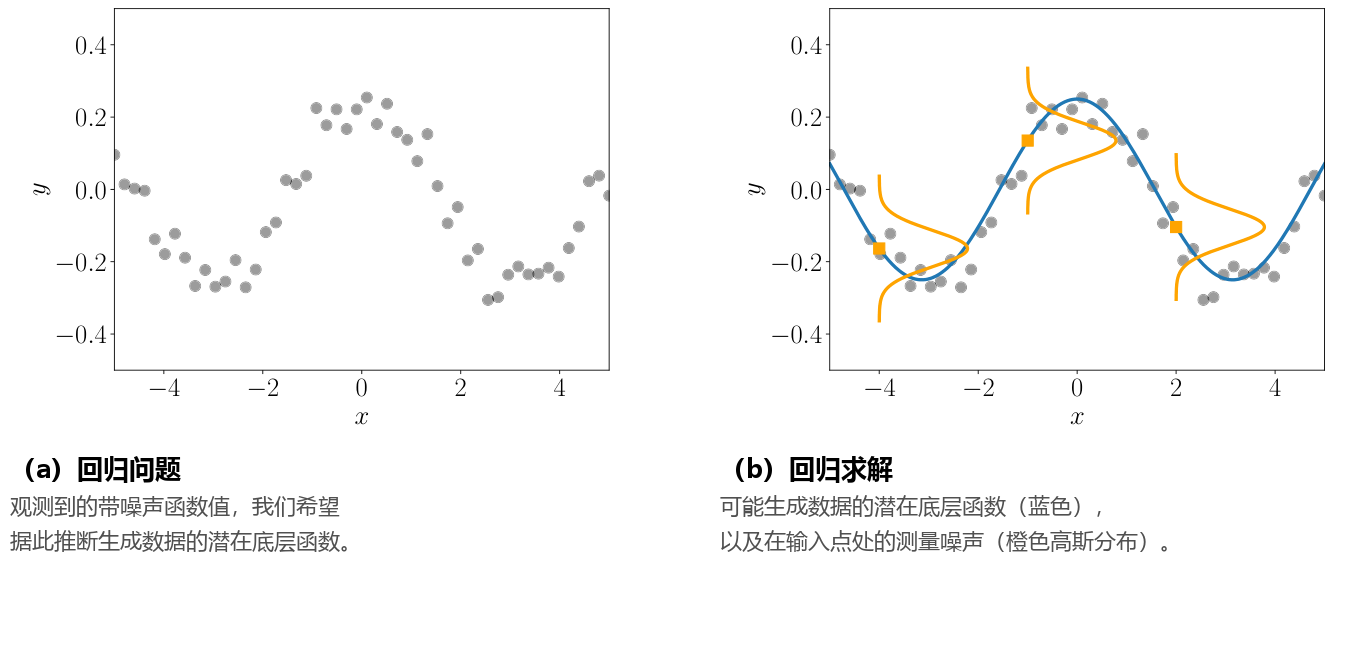
\includegraphics[width=0.92\textwidth,keepaspectratio]{docs/images/Figure9.1.png}
\caption*{\refstepcounter{figcounter}\label{fig:9-1}图~\thefigcounter}
\end{figure}


回归是机器学习中的一个基础核心问题，广泛出现在多种研究领域与实际应用中，包括时间序列分析（如系统辨识）、控制与机器人学（如强化学习、正向/逆向模型学习）、连续优化（如线搜索、全局优化）以及深度学习应用（如计算机游戏、语音转文字、图像识别、视频自动标注等）。回归也是许多分类算法的关键组成部分。寻找一个满意的回归函数需要解决一系列问题，主要包括以下几个方面：

\begin{enumerate}
\item \textbf{模型（类型）的选择与回归函数的参数化}：给定数据集，哪些函数类（例如多项式）适合用于对数据进行建模？我们应当选择哪种具体的参数化形式（例如多项式的阶数）？正如 8.6 节所讨论的， \emph{模型选择（model selection）} 允许我们比较不同的模型，从而找到能够合理解释训练数据的最简模型。通常，噪声类型的选择也属于“模型选择”的范畴，但在本章中我们将噪声固定为高斯噪声。
\item \textbf{寻找优良参数}：选定回归函数的模型后，我们如何寻找优良的模型参数？在此，我们需要考察不同的损失/目标函数（它们定义了何为“拟合得好”）以及能够最小化该损失的优化算法。
\item \textbf{过拟合与模型选择}：当回归函数拟合训练数据“过好”，却无法泛化到未见过的测试数据时，就会发生 \emph{过拟合（overfitting）} 。当底层模型（或其参数化）过于灵活和表达能力过强时，通常会发生过拟合（见 8.6 节）。我们将探究其底层成因，并讨论在线性回归背景下缓解过拟合效应的途径。
\item \textbf{损失函数与参数先验之间的联系}：损失函数（优化目标）通常由概率模型激发并导出。我们将探讨优化损失函数与导出这些损失的底层先验假设之间的深刻对应关系。
\item \textbf{不确定性建模}：在任何实际应用中，我们都只能利用有限（尽管可能很大）的训练数据来选择模型类及相应参数。鉴于这些有限的训练数据不可能涵盖所有可能的情景，我们可能希望描述残留的参数不确定性，从而获得模型在测试阶段预测结果的置信度量；训练集越小，不确定性建模就越重要。自洽严谨的不确定性建模赋予了模型预测以置信区间。
\end{enumerate}

在接下来的各节中，我们将系统运用第 3、5、6 和 7 章的数学工具来解决线性回归问题：

\begin{itemize}
\item 在 9.1 节中形式化问题表述；
\item 在 9.2 节中讨论用于寻找最优模型参数的极大似然估计（MLE）与最大后验估计（MAP），并简要剖析泛化误差与过拟合现象；
\item 在 9.3 节中介绍贝叶斯线性回归（Bayesian linear regression），它允许我们在更高层次上对模型参数进行概率推理，从而消除极大似然和 MAP 估计中所遇到的一些固有缺陷；
\item 在 9.4 节中从几何角度将极大似然解阐释为正交投影；
\item 在 9.5 节中提供延伸阅读建议。
\end{itemize}

\section*{9.1 问题表述}
\addcontentsline{toc}{section}{9.1 问题表述}
\label{sec:9.1}

由于观测噪声的存在，我们将采用概率方法，并通过似然函数对噪声进行显式建模。更具体地说，贯穿本章，我们考虑具有如下似然函数的回归问题：

\begin{equation}
p(y \mid \boldsymbol{x}) = \mathcal{N}\left(y \mid f(\boldsymbol{x}), \sigma^2\right) .
\tag{9.1}\label{eq:9-1}
\end{equation}

这里，$ \boldsymbol{x} \in \mathbb{R}^D $ 为输入，$ y \in \mathbb{R} $ 为带噪声的函数值（目标标签）。由式~\eqref{eq:9-1}，$ \boldsymbol{x} $ 与 $ y $ 之间的函数关系可以表示为：

\begin{equation}
y = f(\boldsymbol{x}) + \epsilon
\tag{9.2}\label{eq:9-2}
\end{equation}

其中 $ \epsilon \sim \mathcal{N}(0, \sigma^2) $ 是均值为 0、方差为 $ \sigma^2 $ 的独立同分布（i.i.d.）高斯测量噪声。我们的目标是找到一个与生成数据的未知底层函数 $ f $ 接近（相似）且泛化能力良好的函数。

在本章中，我们重点关注 \emph{参数化模型（parametric models）} ，即选择一个参数化函数，并寻找能够“良好运作”以对数据进行建模的参数 $ \boldsymbol{\theta} $。目前，我们假设噪声方差 $ \sigma^2 $ 是已知的，并专注于学习模型参数 $ \boldsymbol{\theta} $。在 \emph{线性回归（linear regression）} 中，我们考虑参数 $ \boldsymbol{\theta} $ 在模型中线性出现的特殊情况。线性回归的一个基础示例由下式给出：

\begin{equation}
p(y \mid \boldsymbol{x}, \boldsymbol{\theta}) = \mathcal{N}\left(y \mid \boldsymbol{x}^\top \boldsymbol{\theta}, \sigma^2\right)
\tag{9.3}\label{eq:9-3}
\end{equation}

\begin{equation}
\iff y = \boldsymbol{x}^\top \boldsymbol{\theta} + \epsilon , \quad \epsilon \sim \mathcal{N}(0, \sigma^2)
\tag{9.4}\label{eq:9-4}
\end{equation}

其中 $ \boldsymbol{\theta} \in \mathbb{R}^D $ 是我们要求解的参数。由式~\eqref{eq:9-4} 描述的函数类是通过原点的直线。在式~\eqref{eq:9-4} 中，我们选择了参数化形式 $ f(\boldsymbol{x}) = \boldsymbol{x}^\top \boldsymbol{\theta} $。

\emph{狄拉克 $ \delta $ 函数（Dirac delta function）在除单点之外的所有位置均为零，且其全域积分为 1。它可以被视为高斯分布在 $ \sigma^2 \to 0 $ 极限下的形式。}

式~\eqref{eq:9-3} 中的 \emph{似然（likelihood）} 是在 $ \boldsymbol{x}^\top \boldsymbol{\theta} $ 处评估的 $ y $ 的概率密度函数。需要注意的是，唯一的不确定性来源是观测噪声（因为在式~\eqref{eq:9-3} 中假设 $ \boldsymbol{x} $ 和 $ \boldsymbol{\theta} $ 都是已知的）。如果没有观测噪声，$ \boldsymbol{x} $ 与 $ y $ 之间的关系将是确定性的，此时式~\eqref{eq:9-3} 将退化为一个狄拉克 $ \delta $ 函数。

\begin{notebox}
\textbf{例 9.1}
\end{notebox}

\begin{notebox}
当 $ x, \theta \in \mathbb{R} $ 时，式~\eqref{eq:9-4} 中的线性回归模型描述了直线（线性函数），参数 $ \theta $ 即为直线的斜率。图~\ref{fig:9-2}(a) 展示了对应不同 $ \theta $ 取值的一些函数示例。
\end{notebox}

\emph{“线性回归”指的是在参数上呈线性的模型。}

式~\eqref{eq:9-3}–(9.4) 中的线性回归模型不仅在参数上呈线性，在输入 $ \boldsymbol{x} $ 上也是线性的。图~\ref{fig:9-2}(a) 展示了此类函数的示例。稍后我们将看到，对于非线性特征变换 $ \boldsymbol{\phi} $，形式为 $ y = \boldsymbol{\phi}^\top(\boldsymbol{x})\boldsymbol{\theta} $ 的模型同样是线性回归模型，因为“线性回归”指的是在 \textbf{参数} 上呈线性的模型，即通过输入特征的线性组合来描述函数的模型。在这里，“特征”是输入 $ \boldsymbol{x} $ 的一种表示 $ \boldsymbol{\phi}(\boldsymbol{x}) $。


\begin{figure}[H]
\centering
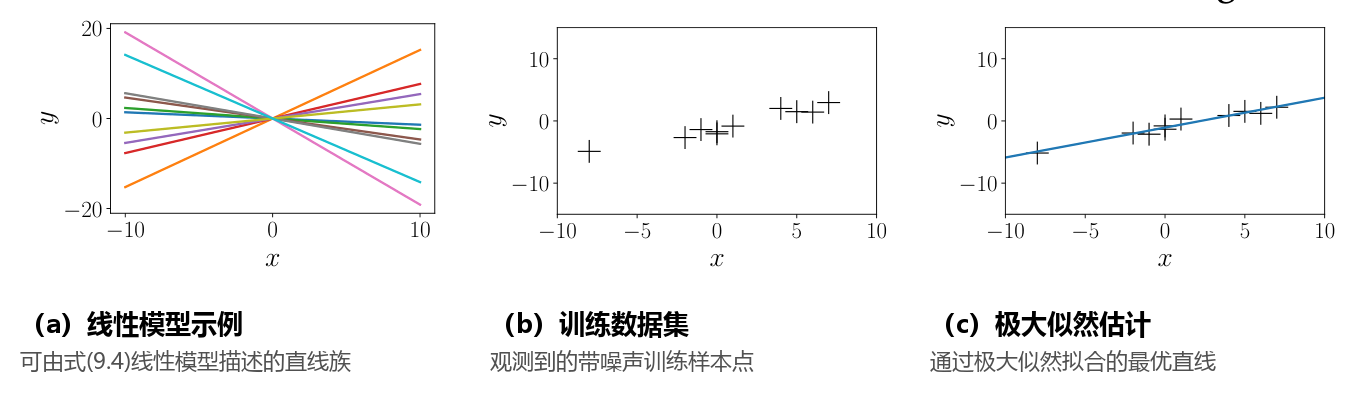
\includegraphics[width=0.92\textwidth,keepaspectratio]{docs/images/Figure9.2.png}
\caption*{\refstepcounter{figcounter}\label{fig:9-2}图~\thefigcounter}
\end{figure}


在下文中，我们将更详细地讨论如何寻找优良的参数 $ \boldsymbol{\theta} $，以及如何评估参数集是否“表现良好”。目前，我们仍假设噪声方差 $ \sigma^2 $ 是已知的。

\section*{9.2 参数估计}
\addcontentsline{toc}{section}{9.2 参数估计}
\label{sec:9.2}

考虑式 (9.4) 中的线性回归设定，并假设给定一个训练集 $ \mathcal{D} := \{(\boldsymbol{x}_1, y_1), \ldots, (\boldsymbol{x}_N, y_N)\} $，其中包含 $ N $ 个输入 $ \boldsymbol{x}_n \in \mathbb{R}^D $ 及对应的观测/目标值 $ y_n \in \mathbb{R} $（$ n = 1, \ldots, N $）。对应的概率图模型如图 9.3 所示。


\begin{figure}[H]
\centering
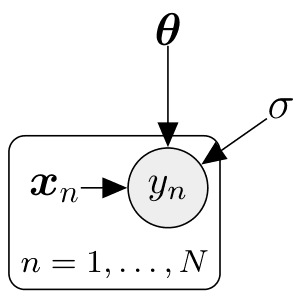
\includegraphics[width=320pt,keepaspectratio]{docs/images/Figure9.3.png}
\caption*{图 9.3}
\end{figure}


请注意，在给定各自的输入 $ \boldsymbol{x}_i, \boldsymbol{x}_j $ 以及参数 $ \boldsymbol{\theta} $ 的条件下，$ y_i $ 与 $ y_j $ 是条件独立的，因此似然函数可以按如下方式因式分解：

\begin{equation}
p(\mathcal{Y} \mid \mathcal{X}, \boldsymbol{\theta}) = p(y_1, \ldots, y_N \mid \boldsymbol{x}_1, \ldots, \boldsymbol{x}_N, \boldsymbol{\theta})
\tag{9.5a}
\end{equation}

\begin{equation}
= \prod_{n=1}^N p(y_n \mid \boldsymbol{x}_n, \boldsymbol{\theta}) = \prod_{n=1}^N \mathcal{N}\left(y_n \mid \boldsymbol{x}_n^\top \boldsymbol{\theta}, \sigma^2\right)
\tag{9.5b}
\end{equation}

其中我们将 $ \mathcal{X} := \{\boldsymbol{x}_1, \ldots, \boldsymbol{x}_N\} $ 和 $ \mathcal{Y} := \{y_1, \ldots, y_N\} $ 分别定义为训练输入集合与对应的目标值集合。由于噪声分布为高斯分布，似然函数及其各个因子 $ p(y_n \mid \boldsymbol{x}_n, \boldsymbol{\theta}) $ 均为高斯分布；参见式 (9.3)。

在下文中，我们将讨论如何为线性回归模型 (9.4) 寻找最优参数 $ \boldsymbol{\theta}^* \in \mathbb{R}^D $。一旦找到参数 $ \boldsymbol{\theta}^* $，我们便可以将该参数估计代入式 (9.4) 来预测函数值，从而对于任意测试输入 $ \boldsymbol{x}_* $，对应目标值 $ y_* $ 的分布为：

\begin{equation}
p(y_* \mid \boldsymbol{x}_*, \boldsymbol{\theta}^*) = \mathcal{N}\left(y_* \mid \boldsymbol{x}_*^\top \boldsymbol{\theta}^*, \sigma^2\right) .
\tag{9.6}
\end{equation}

接下来，我们将首先考察通过最大化似然函数来进行参数估计的方法，我们在 8.3 节中已经对该主题做过一定程度的探讨。

\medskip\hrule\medskip

\section*{9.2.1 极大似然估计}
\addcontentsline{toc}{subsection}{9.2.1 极大似然估计}

寻找所需参数 $ \boldsymbol{\theta}_{\text{ML}} $ 的一种广泛采用的方法是 \emph{极大似然估计（maximum likelihood estimation）} ，即寻找使似然函数 (9.5b) 最大化的参数 $ \boldsymbol{\theta}_{\text{ML}} $。直观上，最大化似然意味着在给定模型参数的条件下，最大化训练数据的预测概率分布。我们通过下式获得极大似然参数：

\begin{equation}
\boldsymbol{\theta}_{\text{ML}} = \arg\max_{\boldsymbol{\theta}} p(\mathcal{Y} \mid \mathcal{X}, \boldsymbol{\theta}) .
\tag{9.7}
\end{equation}

\emph{备注} 。似然 $ p(y \mid \boldsymbol{x}, \boldsymbol{\theta}) $ 并不是关于 $ \boldsymbol{\theta} $ 的概率分布：它仅仅是参数 $ \boldsymbol{\theta} $ 的函数，其对 $ \boldsymbol{\theta} $ 的积分并不为 1（即它是未归一化的），甚至关于 $ \boldsymbol{\theta} $ 可能根本不可积。然而，式 (9.7) 中的似然关于 $ y $ 是一个归一化的概率分布。

为了寻找使似然最大化的参数 $ \boldsymbol{\theta}_{\text{ML}} $，通常执行梯度上升法（或对负似然执行梯度下降法）。然而，在我们这里考虑的线性回归情形中，存在解析闭式解，这使得迭代梯度下降变得不再必要。在实践中，我们通常不对似然函数直接求最大值，而是对似然函数取对数变换，并最小化 \emph{负对数似然（negative log-likelihood）} 。

\emph{备注} （对数变换） 。由于似然函数 (9.5b) 是 $ N $ 个高斯分布的连乘积，对数变换之所以极其有用，是因为：(a) 它不会遭遇数值下溢问题；(b) 求导法则将变得更加简便。更具体地说，当数据点数量 $ N $ 很大时，将 $ N $ 个概率相乘会导致严重的数值下溢，因为计算机无法精确表示诸如 $ 10^{-256} $ 这样极小的正浮点数。此外，对数变换将连乘积转化为对数概率的连加和，使得对应的梯度等于各个单项梯度的简单求和，而无需反复应用乘积法则（式 (5.46)）来计算 $ N $ 个项乘积的高阶梯度。

为了寻找线性回归问题的最优参数 $ \boldsymbol{\theta}_{\text{ML}} $，我们最小化负对数似然：

\begin{equation}
-\log p(\mathcal{Y} \mid \mathcal{X}, \boldsymbol{\theta}) = -\log \prod_{n=1}^N p(y_n \mid \boldsymbol{x}_n, \boldsymbol{\theta}) = -\sum_{n=1}^N \log p(y_n \mid \boldsymbol{x}_n, \boldsymbol{\theta})
\tag{9.8}
\end{equation}

其中我们利用了基于训练集独立性假设而使似然函数 (9.5b) 能够在各数据点上因式分解的性质。在线性回归模型 (9.4) 中，似然为高斯分布（源于高斯加性噪声项），因此我们得到：

\begin{equation}
\log p(y_n \mid \boldsymbol{x}_n, \boldsymbol{\theta}) = -\frac{1}{2\sigma^2}(y_n - \boldsymbol{x}_n^\top \boldsymbol{\theta})^2 + \text{const}
\tag{9.9}
\end{equation}

其中常数项包含了所有与 $ \boldsymbol{\theta} $ 无关的项。将式 (9.9) 代入负对数似然 (9.8) 中，我们得到如下目标函数（忽略常数项）：

\begin{equation}
L(\boldsymbol{\theta}) := \frac{1}{2\sigma^2}\sum_{n=1}^N (y_n - \boldsymbol{x}_n^\top \boldsymbol{\theta})^2
\tag{9.10a}
\end{equation}

\begin{equation}
= \frac{1}{2\sigma^2}(\boldsymbol{y} - \boldsymbol{X}\boldsymbol{\theta})^\top(\boldsymbol{y} - \boldsymbol{X}\boldsymbol{\theta}) = \frac{1}{2\sigma^2}\|\boldsymbol{y} - \boldsymbol{X}\boldsymbol{\theta}\|^2
\tag{9.10b}
\end{equation}

其中我们将 \emph{设计矩阵（design matrix）} 定义为收集所有训练输入的矩阵 $ \boldsymbol{X} := [\boldsymbol{x}_1, \ldots, \boldsymbol{x}_N]^\top \in \mathbb{R}^{N \times D} $，将目标向量定义为收集所有训练标签的向量 $ \boldsymbol{y} := [y_1, \ldots, y_N]^\top \in \mathbb{R}^N $。请注意，设计矩阵 $ \boldsymbol{X} $ 的第 $ n $ 行对应于第 $ n $ 个训练输入 $ \boldsymbol{x}_n $。在式 (9.10b) 中，我们利用了观测值 $ y_n $ 与对应模型预测值 $ \boldsymbol{x}_n^\top \boldsymbol{\theta} $ 之间的残差平方和等于向量 $ \boldsymbol{y} $ 与 $ \boldsymbol{X}\boldsymbol{\theta} $ 之间的欧几里得平方距离这一事实（回顾 3.1 节，当我们选择点积作为内积时，$ \|\boldsymbol{x}\|^2 = \boldsymbol{x}^\top \boldsymbol{x} $）。负对数似然函数有时也称为 \emph{误差函数（error function）} 。

借助式 (9.10b)，我们获得了需要优化的负对数似然函数的具体形式。我们立即可以看出式 (9.10b) 关于 $ \boldsymbol{\theta} $ 是二次的。这意味着我们可以找到唯一的全局最优解 $ \boldsymbol{\theta}_{\text{ML}} $ 来最小化负对数似然 $ L $。我们可以通过计算 $ L $ 的梯度、令其为 $ \boldsymbol{0} $ 并求解 $ \boldsymbol{\theta} $ 来求得全局极小值。

运用第 5 章的结果，我们计算 $ L $ 关于参数 $ \boldsymbol{\theta} $ 的梯度为：

\begin{equation}
\begin{adjustbox}{max width=\linewidth}
\frac{\mathrm{d}L}{\mathrm{d}\boldsymbol{\theta}} = \frac{\mathrm{d}}{\mathrm{d}\boldsymbol{\theta}}\left[ \frac{1}{2\sigma^2}(\boldsymbol{y} - \boldsymbol{X}\boldsymbol{\theta})^\top(\boldsymbol{y} - \boldsymbol{X}\boldsymbol{\theta}) \right]
\end{adjustbox}
\tag{9.11a}
\end{equation}

\begin{equation}
\begin{adjustbox}{max width=\linewidth}
= \frac{1}{2\sigma^2}\frac{\mathrm{d}}{\mathrm{d}\boldsymbol{\theta}}\left[ \boldsymbol{y}^\top\boldsymbol{y} - 2\boldsymbol{y}^\top\boldsymbol{X}\boldsymbol{\theta} + \boldsymbol{\theta}^\top\boldsymbol{X}^\top\boldsymbol{X}\boldsymbol{\theta} \right]
\end{adjustbox}
\tag{9.11b}
\end{equation}

\begin{equation}
= \frac{1}{\sigma^2}(-\boldsymbol{y}^\top\boldsymbol{X} + \boldsymbol{\theta}^\top\boldsymbol{X}^\top\boldsymbol{X}) \in \mathbb{R}^{1 \times D} .
\tag{9.11c}
\end{equation}

极大似然估计量 $ \boldsymbol{\theta}_{\text{ML}} $ 满足一阶必要最优性条件 $ \frac{\mathrm{d}L}{\mathrm{d}\boldsymbol{\theta}} = \boldsymbol{0}^\top $，从而我们得到：

\begin{equation}
\frac{\mathrm{d}L}{\mathrm{d}\boldsymbol{\theta}} = \boldsymbol{0}^\top \overset{(9.11c)}{\iff} \boldsymbol{\theta}_{\text{ML}}^\top \boldsymbol{X}^\top \boldsymbol{X} = \boldsymbol{y}^\top \boldsymbol{X}
\tag{9.12a}
\end{equation}

\begin{equation}
\iff \boldsymbol{\theta}_{\text{ML}}^\top = \boldsymbol{y}^\top \boldsymbol{X}(\boldsymbol{X}^\top \boldsymbol{X})^{-1}
\tag{9.12b}
\end{equation}

\begin{equation}
\iff \boldsymbol{\theta}_{\text{ML}} = (\boldsymbol{X}^\top \boldsymbol{X})^{-1}\boldsymbol{X}^\top \boldsymbol{y} .
\tag{9.12c}
\end{equation}

忽略重复数据点的可能性，当 $ N \geqslant D $（即数据点数量不少于参数个数）且 $ \text{rk}(\boldsymbol{X}) = D $ 时，对称矩阵 $ \boldsymbol{X}^\top \boldsymbol{X} $ 是正定的，因此我们可以在第一个方程两边右乘 $ (\boldsymbol{X}^\top \boldsymbol{X})^{-1} $。

\emph{备注} 。令梯度为 $ \boldsymbol{0}^\top $ 在此处既是必要条件也是充分条件，因为其黑塞矩阵 $ \nabla_{\boldsymbol{\theta}}^2 L(\boldsymbol{\theta}) = \frac{1}{\sigma^2}\boldsymbol{X}^\top \boldsymbol{X} \in \mathbb{R}^{D \times D} $ 是半正定的（当 $ \text{rk}(\boldsymbol{X})=D $ 时严格正定），从而保证求得的驻点是全局极小值点。

\emph{备注} 。式 (9.12c) 中的极大似然解要求我们求解形如 $ \boldsymbol{A}\boldsymbol{\theta} = \boldsymbol{b} $ 的线性方程组（称为 \emph{正规方程组（normal equations）}），其中 $ \boldsymbol{A} = \boldsymbol{X}^\top \boldsymbol{X} $，$ \boldsymbol{b} = \boldsymbol{X}^\top \boldsymbol{y} $。

\begin{notebox}
\textbf{例 9.2（拟合直线）}
\end{notebox}

\begin{notebox}
让我们重新审视图 9.2，在该图中我们的目标是使用极大似然估计将一条直线 $ f(x) = \theta x $（其中 $ \theta $ 为未知斜率）拟合到数据集。该模型类（直线）中的函数示例显示在图 9.2(a) 中。对于图 9.2(b) 所示的数据集，我们利用式 (9.12c) 求解斜率参数 $ \theta $ 的极大似然估计，最终得到图 9.2(c) 中的极大似然线性函数。
\end{notebox}

\subsection*{带有特征映射的极大似然估计}
\addcontentsline{toc}{subsubsection}{带有特征映射的极大似然估计}

到目前为止，我们考虑的是式 (9.4) 所描述的基础线性回归设定，它允许我们使用极大似然估计将直线拟合到数据中。然而，在拟合更具结构性的复杂数据时，单纯的直线表达能力明显不足。幸运的是，线性回归在线性框架内为我们提供了一种拟合非线性函数的强大途径：由于“线性回归”仅指“在参数上呈线性”，我们可以对输入 $ \boldsymbol{x} $ 执行任意非线性变换 $ \boldsymbol{\phi}(\boldsymbol{x}) $，然后再对该变换的各分量进行线性组合。对应的线性回归模型为：

\begin{equation}
\begin{adjustbox}{max width=\linewidth}
p(y \mid \boldsymbol{x}, \boldsymbol{\theta}) = \mathcal{N}\left(y \mid \boldsymbol{\phi}^\top(\boldsymbol{x})\boldsymbol{\theta}, \sigma^2\right) \iff y = \boldsymbol{\phi}^\top(\boldsymbol{x})\boldsymbol{\theta} + \epsilon = \sum_{k=0}^{K-1}\theta_k \phi_k(\boldsymbol{x}) + \epsilon
\end{adjustbox}
\tag{9.13}
\end{equation}

其中 $ \boldsymbol{\phi}: \mathbb{R}^D \to \mathbb{R}^K $ 是输入 $ \boldsymbol{x} $ 的（非线性）特征映射变换，$ \phi_k: \mathbb{R}^D \to \mathbb{R} $ 是 \emph{特征向量（feature vector）} $ \boldsymbol{\phi} $ 的第 $ k $ 个分量。需要重点强调的是，模型参数 $ \boldsymbol{\theta} $ 在模型中仍然仅以线性形式出现。

\begin{notebox}
\textbf{例 9.3（多项式回归）}
\end{notebox}

\begin{notebox}
考虑回归问题 $ y = \boldsymbol{\phi}^\top(x)\boldsymbol{\theta} + \epsilon $，其中 $ x \in \mathbb{R} $，$ \boldsymbol{\theta} \in \mathbb{R}^K $。在此情境下常用的特征变换为单项式基函数：
\end{notebox}

\begin{notebox}
\begin{equation}
\boldsymbol{\phi}(x) = \begin{bmatrix} \phi_0(x) \\ \phi_1(x) \\ \vdots \\ \phi_{K-1}(x) \end{bmatrix} = \begin{bmatrix} 1 \\ x \\ x^2 \\ x^3 \\ \vdots \\ x^{K-1} \end{bmatrix} \in \mathbb{R}^K .
\tag{9.14}
\end{equation}
\end{notebox}

\begin{notebox}
这意味着我们将原始一维输入空间“提升”（lift）到了由所有单项式 $ x^k $（$ k = 0, \ldots, K-1 $）构成的 $ K $ 维特征空间中。借助这些特征，我们可以在线性回归的统一框架下对阶数不超过 $ K-1 $ 的多项式进行建模：一个 $ K-1 $ 阶多项式表示为：
\end{notebox}

\begin{notebox}
\begin{equation}
f(x) = \sum_{k=0}^{K-1}\theta_k x^k = \boldsymbol{\phi}^\top(x)\boldsymbol{\theta}
\tag{9.15}
\end{equation}
\end{notebox}

\begin{notebox}
其中 $ \boldsymbol{\phi} $ 由式 (9.14) 定义，$ \boldsymbol{\theta} = [\theta_0, \ldots, \theta_{K-1}]^\top \in \mathbb{R}^K $ 包含了全部（线性）参数 $ \theta_k $。
\end{notebox}

现在让我们考察线性回归模型 (9.13) 中参数 $ \boldsymbol{\theta} $ 的极大似然估计。我们考虑训练输入 $ \boldsymbol{x}_n \in \mathbb{R}^D $ 及目标值 $ y_n \in \mathbb{R} $（$ n = 1, \ldots, N $），并将 \emph{特征矩阵（feature matrix）} （亦称设计矩阵）定义为：

\begin{equation}
\begin{adjustbox}{max width=\linewidth}
\boldsymbol{\Phi} := \begin{bmatrix} \boldsymbol{\phi}^\top(\boldsymbol{x}_1) \\ \vdots \\ \boldsymbol{\phi}^\top(\boldsymbol{x}_N) \end{bmatrix} = \begin{bmatrix} \phi_0(\boldsymbol{x}_1) & \cdots & \phi_{K-1}(\boldsymbol{x}_1) \\ \phi_0(\boldsymbol{x}_2) & \cdots & \phi_{K-1}(\boldsymbol{x}_2) \\ \vdots & & \vdots \\ \phi_0(\boldsymbol{x}_N) & \cdots & \phi_{K-1}(\boldsymbol{x}_N) \end{bmatrix} \in \mathbb{R}^{N \times K}
\end{adjustbox}
\tag{9.16}
\end{equation}

其中 $ \Phi_{ij} = \phi_j(\boldsymbol{x}_i) $，$ \phi_j: \mathbb{R}^D \to \mathbb{R} $。

\begin{notebox}
\textbf{例 9.4（二次多项式的特征矩阵）}
\end{notebox}

\begin{notebox}
对于二次多项式及 $ N $ 个一维训练数据点 $ x_n \in \mathbb{R} $（$ n = 1, \ldots, N $），其特征矩阵为：
\end{notebox}

\begin{notebox}
\begin{equation}
\boldsymbol{\Phi} = \begin{bmatrix} 1 & x_1 & x_1^2 \\ 1 & x_2 & x_2^2 \\ \vdots & \vdots & \vdots \\ 1 & x_N & x_N^2 \end{bmatrix} .
\tag{9.17}
\end{equation}
\end{notebox}

利用式 (9.16) 中定义的特征矩阵 $ \boldsymbol{\Phi} $，线性回归模型 (9.13) 的负对数似然可紧凑写作：

\begin{equation}
-\log p(\mathcal{Y} \mid \mathcal{X}, \boldsymbol{\theta}) = \frac{1}{2\sigma^2}(\boldsymbol{y} - \boldsymbol{\Phi}\boldsymbol{\theta})^\top(\boldsymbol{y} - \boldsymbol{\Phi}\boldsymbol{\theta}) + \text{const} .
\tag{9.18}
\end{equation}

将式 (9.18) 与未引入特征映射时的负对数似然 (9.10b) 进行对比，我们立刻发现只需将 $ \boldsymbol{X} $ 替换为 $ \boldsymbol{\Phi} $ 即可。由于 $ \boldsymbol{X} $ 和 $ \boldsymbol{\Phi} $ 均独立于我们要优化的参数 $ \boldsymbol{\theta} $，我们立即得出带有非线性特征映射的线性回归问题的极大似然估计解：

\begin{equation}
\boldsymbol{\theta}_{\text{ML}} = (\boldsymbol{\Phi}^\top \boldsymbol{\Phi})^{-1}\boldsymbol{\Phi}^\top \boldsymbol{y} .
\tag{9.19}
\end{equation}

\emph{备注} 。在无特征映射的情形中，我们要求 $ \boldsymbol{X}^\top \boldsymbol{X} $ 可逆，这在 $ \boldsymbol{X} $ 的各列线性无关时成立。在式 (9.19) 中，我们相应地要求 $ \boldsymbol{\Phi}^\top \boldsymbol{\Phi} \in \mathbb{R}^{K \times K} $ 可逆，这当且仅当 $ \text{rk}(\boldsymbol{\Phi}) = K $ 时成立。

\begin{notebox}
\textbf{例 9.5（极大似然多项式拟合）}
\end{notebox}

\begin{notebox}
考虑图 9.4(a) 所示的数据集。该数据集包含 $ N = 10 $ 对数据点 $ (x_n, y_n) $，其中 $ x_n \sim \mathcal{U}[-5, 5] $，$ y_n = -\sin(x_n/5) + \cos(x_n) + \epsilon $，且 $ \epsilon \sim \mathcal{N}(0, 0.2^2) $。
\end{notebox}

\begin{notebox}
我们使用极大似然估计拟合一个 4 次多项式，即参数 $ \boldsymbol{\theta}_{\text{ML}} $ 由式 (9.19) 计算给出。极大似然估计在任意测试输入位置 $ x_* $ 处给出预测函数值 $ \boldsymbol{\phi}^\top(x_*)\boldsymbol{\theta}_{\text{ML}} $。拟合结果如图 9.4(b) 所示。
\end{notebox}


\begin{figure}[H]
\centering
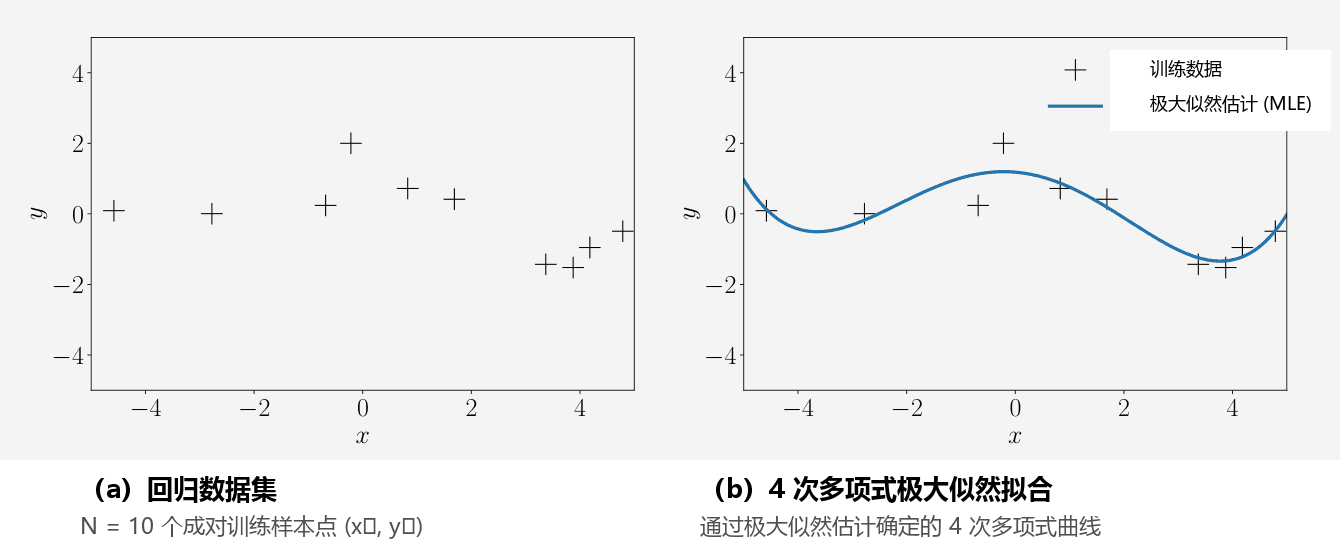
\includegraphics[width=0.92\textwidth,keepaspectratio]{docs/images/Figure9.4.png}
\caption*{图 9.4}
\end{figure}


\subsection*{估计噪声方差}
\addcontentsline{toc}{subsubsection}{估计噪声方差}

迄今为止，我们一直假定噪声方差 $ \sigma^2 $ 是已知的先验常数。然而，我们同样可以利用极大似然原理来获取噪声方差的极大似然估计量 $ \sigma_{\text{ML}}^2 $。为此，我们遵循标准流程：写出关于参数和方差的对数似然，计算其对 $ \sigma^2 > 0 $ 的偏导数，令偏导数为 0 并求解。对数似然由下式给出：

\begin{equation}
\log p(\mathcal{Y} \mid \mathcal{X}, \boldsymbol{\theta}, \sigma^2) = \sum_{n=1}^N \log \mathcal{N}\left(y_n \mid \boldsymbol{\phi}^\top(\boldsymbol{x}_n)\boldsymbol{\theta}, \sigma^2\right)
\tag{9.20a}
\end{equation}

\begin{equation}
= \sum_{n=1}^N \left[ -\frac{1}{2}\log(2\pi) - \frac{1}{2}\log \sigma^2 - \frac{1}{2\sigma^2}(y_n - \boldsymbol{\phi}^\top(\boldsymbol{x}_n)\boldsymbol{\theta})^2 \right]
\tag{9.20b}
\end{equation}

\begin{equation}
= -\frac{N}{2}\log \sigma^2 - \frac{1}{2\sigma^2}\underbrace{\sum_{n=1}^N (y_n - \boldsymbol{\phi}^\top(\boldsymbol{x}_n)\boldsymbol{\theta})^2}_{=: s} + \text{const} .
\tag{9.20c}
\end{equation}

对数似然关于 $ \sigma^2 $ 的偏导数为：

\begin{equation}
\frac{\partial \log p(\mathcal{Y} \mid \mathcal{X}, \boldsymbol{\theta}, \sigma^2)}{\partial \sigma^2} = -\frac{N}{2\sigma^2} + \frac{1}{2\sigma^4}s = 0
\tag{9.21a}
\end{equation}

\begin{equation}
\iff \frac{N}{2\sigma^2} = \frac{s}{2\sigma^4}
\tag{9.21b}
\end{equation}

由此我们解出噪声方差的极大似然估计：

\begin{equation}
\sigma_{\text{ML}}^2 = \frac{s}{N} = \frac{1}{N}\sum_{n=1}^N (y_n - \boldsymbol{\phi}^\top(\boldsymbol{x}_n)\boldsymbol{\theta})^2 .
\tag{9.22}
\end{equation}

因此，噪声方差的极大似然估计正是无噪声模型预测值 $ \boldsymbol{\phi}^\top(\boldsymbol{x}_n)\boldsymbol{\theta} $ 与相应带噪声观测值 $ y_n $ 之间残差平方的 \emph{经验均值（empirical mean）} 。

\medskip\hrule\medskip

\section*{9.2.2 线性回归中的过拟合}
\addcontentsline{toc}{subsection}{9.2.2 线性回归中的过拟合}

我们刚才讨论了如何使用极大似然估计将线性模型（例如多项式）拟合到数据中。我们可以通过计算产生的误差/损失来评估模型的质量。一种方法是计算式 (9.10b) 的负对数似然（我们正是通过最小化该目标来确定极大似然估计量的）。或者，鉴于噪声参数 $ \sigma^2 $ 不是模型自由参数，我们可以忽略缩放系数 $ 1/\sigma^2 $，从而得到平方误差损失函数 $ \|\boldsymbol{y} - \boldsymbol{\Phi}\boldsymbol{\theta}\|^2 $。与单纯使用平方损失相比，人们在实践中更常用 \emph{均方根误差（root mean square error, RMSE）} ：

\begin{equation}
\text{RMSE} := \sqrt{\frac{1}{N}\|\boldsymbol{y} - \boldsymbol{\Phi}\boldsymbol{\theta}\|^2} = \sqrt{\frac{1}{N}\sum_{n=1}^N (y_n - \boldsymbol{\phi}^\top(\boldsymbol{x}_n)\boldsymbol{\theta})^2}
\tag{9.23}
\end{equation}

RMSE 的优势在于：(a) 允许我们在样本规模不同、包含不同数据量的数据集之间公平比较误差；(b) 具有与观测函数值 $ y_n $ 完全相同的尺度和物理量纲单位。例如，若我们拟合一个将邮政编码（输入 $ \boldsymbol{x} $ 为纬度与经度）映射到房屋售价（目标 $ y $ 的单位为欧元）的模型，则 RMSE 的测量单位同样是欧元，而平方误差的单位则是欧元$ ^2 $。如果我们在原始负对数似然 (9.10b) 中保留系数 $ \sigma^2 $，得到的目标函数则是无量纲（unitless）的纯数指标。

在模型选择中（参见 8.6 节），我们可以使用 RMSE（或负对数似然）通过寻找使目标最小化的多项式阶数 $ M $ 来确定最佳的多项式模型。由于多项式阶数是非负整数，我们可以执行暴力网格搜索并枚举所有（合理的）$ M $ 取值。对于规模为 $ N $ 的训练集，测试 $ 0 \leqslant M \leqslant N-1 $ 就足够了。当 $ M < N $ 时，极大似然估计量是唯一的；当 $ M \geqslant N $ 时，参数数量超过了数据点数量，此时我们需要求解一个欠定线性方程组（式 (9.19) 中的 $ \boldsymbol{\Phi}^\top \boldsymbol{\Phi} $ 将不再可逆），从而存在无穷多个可能的极大似然估计量。


\begin{figure}[H]
\centering
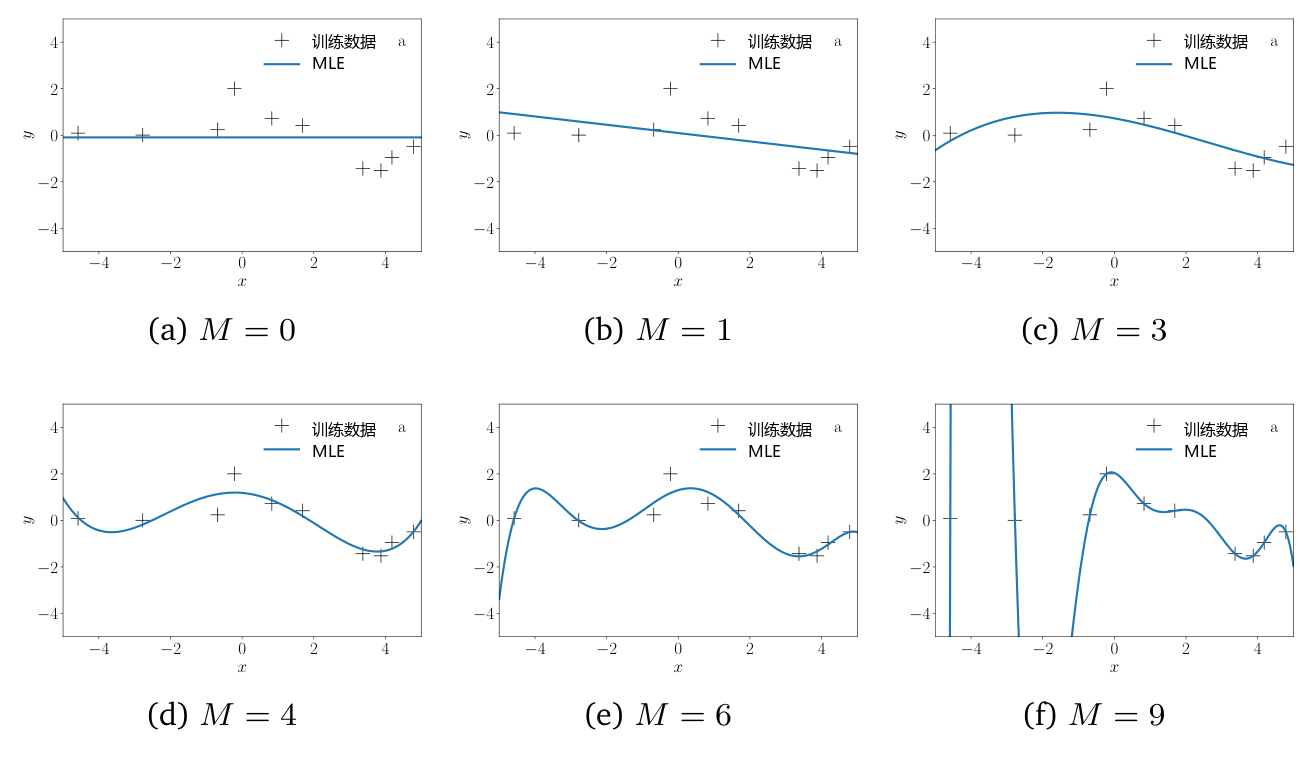
\includegraphics[width=0.92\textwidth,keepaspectratio]{docs/images/Figure9.5.png}
\caption*{图 9.5}
\end{figure}


图 9.5 展示了针对图 9.4(a) 中 $ N = 10 $ 个观测数据点，通过极大似然估计确定的若干不同阶数的多项式拟合曲线。我们注意到：

\begin{itemize}
\item 低阶多项式（例如常数 $ M = 0 $ 或线性 $ M = 1 $）拟合效果很差，无法捕捉真实底层函数的特征；
\item 对于中等阶数 $ M = 3, 4, 5 $，拟合曲线十分合情合理，平滑地穿过了数据点分布的主要趋势；
\item 当多项式阶数进一步增加时，训练数据上的拟合看起来越来越完美。在 $ M = N-1 = 9 $ 的极端情况下，函数曲线完美穿过了每一个训练样本点！然而，这些高阶多项式在样本点之间产生了剧烈的振荡，完全无法代表生成数据的真实底层函数，即发生了严重的 \emph{过拟合（overfitting）} 。
\end{itemize}

请牢记，机器学习的终极目标是在未见过的测试新数据上做出准确预测，从而实现良好的泛化能力。为了定量评估泛化性能对多项式阶数 $ M $ 的依赖性，我们引入一个由 200 个数据点组成的独立测试集，该测试集使用与生成训练集完全相同的底层函数与噪声机制生成。测试输入选取为区间 $ [-5, 5] $ 内均匀分布的 200 个网格点。对于每一个 $ M $，我们分别评估训练数据和测试数据上的 RMSE (9.23)。


\begin{figure}[H]
\centering
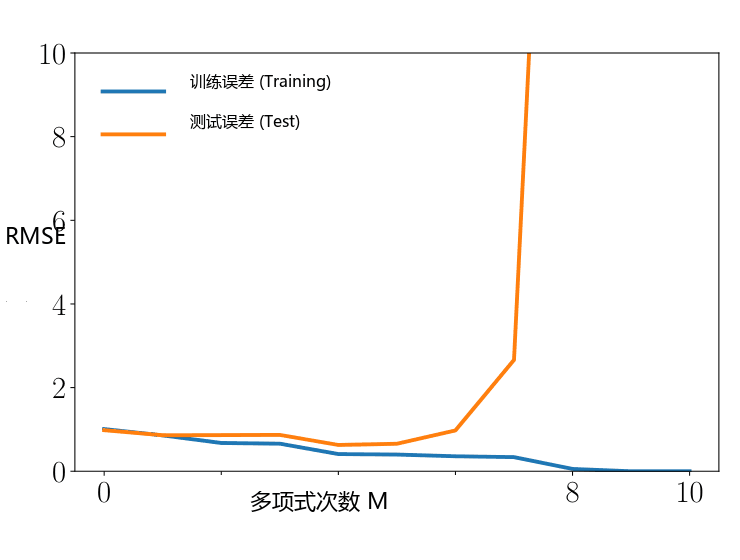
\includegraphics[width=0.92\textwidth,keepaspectratio]{docs/images/Figure9.6.png}
\caption*{图 9.6}
\end{figure}


考察作为泛化性能定性指标的测试误差，我们发现：

\begin{itemize}
\item 如图 9.6 所示，最初随着多项式阶数增加，测试误差（橙色曲线）迅速下降；
\item 在 4 阶多项式附近，测试误差达到较低值并在 5 阶之前保持相对平稳；
\item 然而，从 6 阶开始，测试误差急剧飙升，更高阶的多项式表现出极差的泛化能力。
\end{itemize}

与此同时，训练误差（图 9.6 中的蓝色曲线）随着多项式阶数的增加而单调非递增。在本示例中，最优的泛化效果（即测试误差最低点）在阶数 $ M = 4 $ 处取得。

\medskip\hrule\medskip

\section*{9.2.3 最大后验估计}
\addcontentsline{toc}{subsection}{9.2.3 最大后验估计}

我们刚刚看到，极大似然估计极易遭受过拟合问题。当发生过拟合时，我们常常会观察到模型参数的数值绝对值变得异常庞大（Bishop, 2006）。

为了抑制参数绝对值过度膨胀的现象，我们可以在参数上引入一个 \emph{先验分布（prior distribution）} $ p(\boldsymbol{\theta}) $。先验分布显式地编码了在看到任何数据之前，哪些参数取值在常理上是可信且合理的。例如，对单个参数 $ \theta $ 赋予高斯先验 $ p(\theta) = \mathcal{N}(0, 1) $ 表明我们预期该参数取值以 95\% 的概率落在均值两侧两个标准差区间 $ [-2, 2] $ 内。

一旦获取了观测数据集 $ \mathcal{X}, \mathcal{Y} $，我们不再单纯最大化似然，而是寻找使 \emph{后验分布（posterior distribution）} $ p(\boldsymbol{\theta} \mid \mathcal{X}, \mathcal{Y}) $ 最大化的参数。这一过程被称为 \emph{最大后验估计（maximum a posteriori estimation, MAP）} 。

给定训练数据 $ \mathcal{X}, \mathcal{Y} $，参数 $ \boldsymbol{\theta} $ 的后验分布通过贝叶斯定理（6.3 节）求得：

\begin{equation}
p(\boldsymbol{\theta} \mid \mathcal{X}, \mathcal{Y}) = \frac{p(\mathcal{Y} \mid \mathcal{X}, \boldsymbol{\theta})p(\boldsymbol{\theta})}{p(\mathcal{Y} \mid \mathcal{X})} .
\tag{9.24}
\end{equation}

由于后验分布显式依赖于参数先验 $ p(\boldsymbol{\theta}) $，先验自然会对最大化后验所得的最优参数矢量产生决定性的调节作用。使后验分布 (9.24) 最大化的参数矢量 $ \boldsymbol{\theta}_{\text{MAP}} $ 即为 MAP 估计量。

为了求得 MAP 估计量，我们采取与极大似然估计极为相似的步骤。首先对后验概率取对数，得到对数后验：

\begin{equation}
\log p(\boldsymbol{\theta} \mid \mathcal{X}, \mathcal{Y}) = \log p(\mathcal{Y} \mid \mathcal{X}, \boldsymbol{\theta}) + \log p(\boldsymbol{\theta}) + \text{const}
\tag{9.25}
\end{equation}

其中常数项包含了所有与 $ \boldsymbol{\theta} $ 无关的项。我们看到，式 (9.25) 中的对数后验恰好是对数似然与对数先验的代数和，因此 MAP 估计本质上是先验（观测数据前我们对合理解的主观设定）与依赖于具体数据的似然之间的一种“折衷妥协”。

为了求得 MAP 估计量 $ \boldsymbol{\theta}_{\text{MAP}} $，我们最小化关于 $ \boldsymbol{\theta} $ 的负对数后验分布，即求解：

\begin{equation}
\boldsymbol{\theta}_{\text{MAP}} \in \arg\min_{\boldsymbol{\theta}} \left\{ -\log p(\mathcal{Y} \mid \mathcal{X}, \boldsymbol{\theta}) - \log p(\boldsymbol{\theta}) \right\} .
\tag{9.26}
\end{equation}

负对数后验关于 $ \boldsymbol{\theta} $ 的梯度为：

\begin{equation}
\begin{adjustbox}{max width=\linewidth}
-\frac{\mathrm{d}\log p(\boldsymbol{\theta} \mid \mathcal{X}, \mathcal{Y})}{\mathrm{d}\boldsymbol{\theta}} = -\frac{\mathrm{d}\log p(\mathcal{Y} \mid \mathcal{X}, \boldsymbol{\theta})}{\mathrm{d}\boldsymbol{\theta}} - \frac{\mathrm{d}\log p(\boldsymbol{\theta})}{\mathrm{d}\boldsymbol{\theta}}
\end{adjustbox}
\tag{9.27}
\end{equation}

其中等号右侧第一项正是我们在式 (9.11c) 中求得的负对数似然的梯度。

若在参数 $ \boldsymbol{\theta} $ 上赋予（共轭）高斯先验 $ p(\boldsymbol{\theta}) = \mathcal{N}(\boldsymbol{0}, b^2\boldsymbol{I}) $，对于线性回归设定 (9.13)，我们得到具体的负对数后验表达式：

\begin{equation}
\begin{adjustbox}{max width=\linewidth}
-\log p(\boldsymbol{\theta} \mid \mathcal{X}, \mathcal{Y}) = \frac{1}{2\sigma^2}(\boldsymbol{y} - \boldsymbol{\Phi}\boldsymbol{\theta})^\top(\boldsymbol{y} - \boldsymbol{\Phi}\boldsymbol{\theta}) + \frac{1}{2b^2}\boldsymbol{\theta}^\top \boldsymbol{\theta} + \text{const} .
\end{adjustbox}
\tag{9.28}
\end{equation}

在此，第一项对应于对数似然的贡献，而第二项则来源于对数先验。此时，对数后验关于参数 $ \boldsymbol{\theta} $ 的梯度为：

\begin{equation}
\begin{adjustbox}{max width=\linewidth}
-\frac{\mathrm{d}\log p(\boldsymbol{\theta} \mid \mathcal{X}, \mathcal{Y})}{\mathrm{d}\boldsymbol{\theta}} = \frac{1}{\sigma^2}(\boldsymbol{\theta}^\top \boldsymbol{\Phi}^\top \boldsymbol{\Phi} - \boldsymbol{y}^\top \boldsymbol{\Phi}) + \frac{1}{b^2}\boldsymbol{\theta}^\top .
\end{adjustbox}
\tag{9.29}
\end{equation}

令该梯度为 $ \boldsymbol{0}^\top $ 并求解 $ \boldsymbol{\theta}_{\text{MAP}} $：

\begin{equation}
\frac{1}{\sigma^2}(\boldsymbol{\theta}^\top \boldsymbol{\Phi}^\top \boldsymbol{\Phi} - \boldsymbol{y}^\top \boldsymbol{\Phi}) + \frac{1}{b^2}\boldsymbol{\theta}^\top = \boldsymbol{0}^\top
\tag{9.30a}
\end{equation}

\begin{equation}
\iff \boldsymbol{\theta}^\top \left( \frac{1}{\sigma^2}\boldsymbol{\Phi}^\top \boldsymbol{\Phi} + \frac{1}{b^2}\boldsymbol{I} \right) - \frac{1}{\sigma^2}\boldsymbol{y}^\top \boldsymbol{\Phi} = \boldsymbol{0}^\top
\tag{9.30b}
\end{equation}

\begin{equation}
\iff \boldsymbol{\theta}^\top \left( \boldsymbol{\Phi}^\top \boldsymbol{\Phi} + \frac{\sigma^2}{b^2}\boldsymbol{I} \right) = \boldsymbol{y}^\top \boldsymbol{\Phi}
\tag{9.30c}
\end{equation}

\begin{equation}
\iff \boldsymbol{\theta}^\top = \boldsymbol{y}^\top \boldsymbol{\Phi}\left( \boldsymbol{\Phi}^\top \boldsymbol{\Phi} + \frac{\sigma^2}{b^2}\boldsymbol{I} \right)^{-1} .
\tag{9.30d}
\end{equation}

对最后等式两边进行转置，最终得到 MAP 估计量的解析闭式解：

\begin{equation}
\boldsymbol{\theta}_{\text{MAP}} = \left( \boldsymbol{\Phi}^\top \boldsymbol{\Phi} + \frac{\sigma^2}{b^2}\boldsymbol{I} \right)^{-1}\boldsymbol{\Phi}^\top \boldsymbol{y} .
\tag{9.31}
\end{equation}

将式 (9.31) 中的 MAP 估计与式 (9.19) 中的极大似然估计进行对比，我们清晰地看到两种解之间的唯一差异是在求逆矩阵中增加了额外的项 $ \frac{\sigma^2}{b^2}\boldsymbol{I} $。因为对称矩阵 $ \boldsymbol{\Phi}^\top \boldsymbol{\Phi} $ 是半正定的，而附加项 $ \frac{\sigma^2}{b^2}\boldsymbol{I} $ 是严格正定的（当方差 $ b^2 > 0 $ 时），所以它们的和始终严格正定，从而保证了逆矩阵必然存在，使得 MAP 估计成为线性方程组唯一的稳定解。此外，这一项直接体现了正则化机制的作用。

\begin{notebox}
\textbf{例 9.6（多项式回归的 MAP 估计）}
\end{notebox}

\begin{notebox}
在 9.2.1 节的多项式回归示例中，我们在参数 $ \boldsymbol{\theta} $ 上赋予高斯先验 $ p(\boldsymbol{\theta}) = \mathcal{N}(\boldsymbol{0}, \boldsymbol{I}) $，并根据式 (9.31) 求解 MAP 估计。在图 9.7 中，我们展示了 6 阶（左）和 8 阶（右）多项式的极大似然估计与 MAP 估计对比。对于较低阶的多项式，先验（正则项）的影响微乎其微；但对于高阶多项式，先验能够强有力地约束振荡，使拟合函数保持平滑。虽然 MAP 估计能够拓宽抵御过拟合的边界，但它并非彻底解决该问题的万灵药，我们依然需要更具原则性的系统方法来应对过拟合。
\end{notebox}


\begin{figure}[H]
\centering
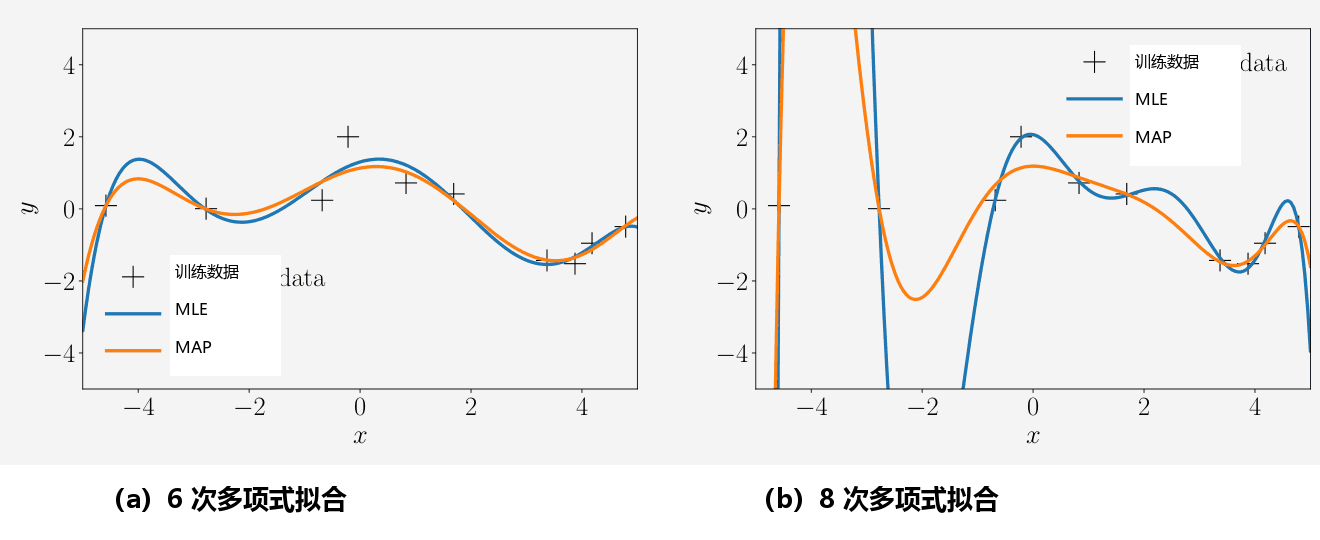
\includegraphics[width=0.92\textwidth,keepaspectratio]{docs/images/Figure9.7.png}
\caption*{图 9.7}
\end{figure}


\medskip\hrule\medskip

\section*{9.2.4 作为正则化的 MAP 估计}
\addcontentsline{toc}{subsection}{9.2.4 作为正则化的 MAP 估计}

除了在参数 $ \boldsymbol{\theta} $ 上引入先验分布之外，另一种缓解过拟合效应的途径是通过 \emph{正则化（regularization）} 手段直接惩罚过大的参数幅度。在 \emph{正则化最小二乘（regularized least squares）} 中，我们考虑如下损失函数并对 $ \boldsymbol{\theta} $ 进行最小化（参见 8.2.3 节）：

\begin{equation}
\|\boldsymbol{y} - \boldsymbol{\Phi}\boldsymbol{\theta}\|^2 + \lambda \|\boldsymbol{\theta}\|_2^2
\tag{9.32}
\end{equation}

其中第一项是数据拟合项（亦称拟合残差项），它正比于负对数似然（参见式 (9.10b)）；第二项称为 \emph{正则化项（regularizer）} ，正则化超参数 $ \lambda \geqslant 0 $ 控制着正则化的“惩罚力度”。

\emph{备注} 。在式 (9.32) 中，我们不仅可以使用欧几里得范数 $ \|\cdot\|_2 $，还可以选用任意的 $ p $-范数 $ \|\cdot\|_p $。在实践中，较小的 $ p $ 值倾向于产生稀疏解。这里的“稀疏”指的是许多参数分量精确为零（$ \theta_d = 0 $），这对于特征与变量选择非常有用。当 $ p = 1 $ 时，该正则化器被称为 LASSO（最小绝对收缩与选择算子），由 Tibshirani (1996) 提出。

式 (9.32) 中的正则化项 $ \lambda \|\boldsymbol{\theta}\|_2^2 $ 可以直接阐释为 MAP 估计中使用的负对数高斯先验（参见式 (9.26)）。具体而言，对于高斯先验 $ p(\boldsymbol{\theta}) = \mathcal{N}(\boldsymbol{0}, b^2\boldsymbol{I}) $，我们有：

\begin{equation}
-\log p(\boldsymbol{\theta}) = \frac{1}{2b^2}\|\boldsymbol{\theta}\|_2^2 + \text{const}
\tag{9.33}
\end{equation}

因此当令 $ \lambda = \frac{\sigma^2}{b^2} $ 时，正则化最小二乘的目标函数与 MAP 估计中的负对数后验函数在常数因子意义下完全等价。

鉴于式 (9.32) 中的正则化最小二乘损失函数由负对数似然与负对数先验两部分紧密构成，最小化该损失所得的解自然与 MAP 估计 (9.31) 具有完全相同的数学形式。更明确地说，最小化正则化最小二乘损失函数得到：

\begin{equation}
\boldsymbol{\theta}_{\text{RLS}} = (\boldsymbol{\Phi}^\top \boldsymbol{\Phi} + \lambda \boldsymbol{I})^{-1}\boldsymbol{\Phi}^\top \boldsymbol{y}
\tag{9.34}
\end{equation}

当设置 $ \lambda = \frac{\sigma^2}{b^2} $ 时，该式与式 (9.31) 中的 MAP 估计完全重合，其中 $ \sigma^2 $ 为观测噪声方差，$ b^2 $ 为各向同性高斯先验 $ p(\boldsymbol{\theta}) = \mathcal{N}(\boldsymbol{0}, b^2\boldsymbol{I}) $ 的先验方差。

迄今为止，我们探讨了基于极大似然估计和 MAP 估计的参数求解，在这两种方法中，我们均通过优化某个目标函数（似然或后验）来求取参数的单一数值点估计 $ \boldsymbol{\theta}^* $。我们发现，极大似然估计和 MAP 估计在小样本或高维模型下均可能诱发过拟合。在下一节中，我们将讨论 \emph{贝叶斯线性回归（Bayesian linear regression）} ，在该框架下，我们运用贝叶斯推断（8.4 节）直接推导未知参数的完整后验概率分布，并随后据此进行预测。具体而言，在进行预测时，我们将对所有合理的可能参数配置进行概率加权平均，而非将目光局限在单一的点估计上。

\section*{9.3 贝叶斯线性回归}
\addcontentsline{toc}{section}{9.3 贝叶斯线性回归}
\label{sec:9.3}

在前面两节中，我们考察了通过极大似然估计或 MAP 估计来估计模型参数 $ \boldsymbol{\theta} $ 的线性回归方法。我们发现，极大似然估计极易导致严重的过拟合，特别是在小数据量的情形下；MAP 估计通过在参数上引入先验分布起到正则化作用，从而缓解了这一问题。

\emph{贝叶斯线性回归（Bayesian linear regression）} 将参数先验的思想更进一步：它甚至不再尝试计算参数的单一数值点估计，而是在进行预测时将参数的完整后验概率分布全面考虑在内。这意味着我们不再拟合任何单一参数值，而是（依据后验分布）对所有合理解的预测结果进行加权平均。

\medskip\hrule\medskip

\section*{9.3.1 模型}
\addcontentsline{toc}{subsection}{9.3.1 模型}

在贝叶斯线性回归中，我们考虑如下模型设定：

\begin{equation}
\textcn{先验：} \quad p(\boldsymbol{\theta}) = \mathcal{N}\left(\boldsymbol{\theta} \mid \boldsymbol{m}_0, \boldsymbol{S}_0\right)
\tag{9.35}
\end{equation}

\begin{equation*}
\textcn{似然：} \quad p(y \mid \boldsymbol{x}, \boldsymbol{\theta}) = \mathcal{N}\left(y \mid \boldsymbol{\phi}^\top(\boldsymbol{x})\boldsymbol{\theta}, \sigma^2\right)
\end{equation*}

在此，我们在参数 $ \boldsymbol{\theta} $ 上显式地赋予高斯先验 $ p(\boldsymbol{\theta}) = \mathcal{N}(\boldsymbol{m}_0, \boldsymbol{S}_0) $，从而将参数矢量转变成了一个随机变量。这使我们能够画出图 9.8 所示的对应概率图模型，其中将 $ \boldsymbol{\theta} $ 的高斯先验参数显式表示了出来。完整的概率模型，即观测随机变量 $ y $ 与未观测随机变量 $ \boldsymbol{\theta} $ 的联合分布为：

\begin{equation}
p(y, \boldsymbol{\theta} \mid \boldsymbol{x}) = p(y \mid \boldsymbol{x}, \boldsymbol{\theta})p(\boldsymbol{\theta}) .
\tag{9.36}
\end{equation}


\begin{figure}[H]
\centering
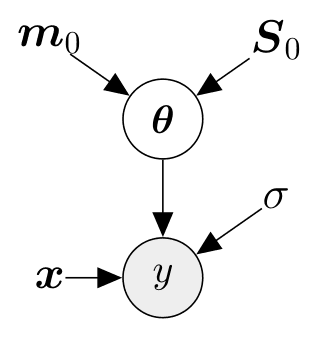
\includegraphics[width=320pt,keepaspectratio]{docs/images/Figure9.8.png}
\caption*{图 9.8}
\end{figure}


\medskip\hrule\medskip

\section*{9.3.2 先验预测}
\addcontentsline{toc}{subsection}{9.3.2 先验预测}

在实际应用中，我们通常对参数值 $ \boldsymbol{\theta} $ 本身并不最感兴趣。相反，我们的核心关注点往往是利用这些参数值做出的预测。在贝叶斯框架下，我们在进行预测时会综合考虑参数的概率分布，并对所有合理的参数取值进行期望平均。更明确地说，为了在任意新测试输入 $ \boldsymbol{x}_* $ 处进行预测，我们将未知参数 $ \boldsymbol{\theta} $ 边缘化积分离出，得到 \emph{先验预测分布（prior predictive distribution）} ：

\begin{equation}
\begin{adjustbox}{max width=\linewidth}
p(y_* \mid \boldsymbol{x}_*) = \int p(y_* \mid \boldsymbol{x}_*, \boldsymbol{\theta})p(\boldsymbol{\theta}) \mathrm{d}\boldsymbol{\theta} = \mathbb{E}_{\boldsymbol{\theta}}\left[ p(y_* \mid \boldsymbol{x}_*, \boldsymbol{\theta}) \right]
\end{adjustbox}
\tag{9.37}
\end{equation}

我们可以将其理解为依据先验分布 $ p(\boldsymbol{\theta}) $ 对所有合理参数 $ \boldsymbol{\theta} $ 下条件预测分布 $ p(y_* \mid \boldsymbol{x}_*, \boldsymbol{\theta}) $ 的加权平均预测。请注意，仅使用先验分布进行预测只需要我们指定测试输入 $ \boldsymbol{x}_* $，而完全不需要任何训练数据。

在我们的模型 (9.35) 中，由于在 $ \boldsymbol{\theta} $ 上选择了共轭（高斯）先验，先验预测分布本身同样是一个高斯分布（并且可以解析闭式计算）：在先验分布 $ p(\boldsymbol{\theta}) = \mathcal{N}(\boldsymbol{m}_0, \boldsymbol{S}_0) $ 下，我们计算得到先验预测分布为：

\begin{equation}
\begin{adjustbox}{max width=\linewidth}
p(y_* \mid \boldsymbol{x}_*) = \mathcal{N}\left(y_* \mid \boldsymbol{\phi}^\top(\boldsymbol{x}_*)\boldsymbol{m}_0, \boldsymbol{\phi}^\top(\boldsymbol{x}_*)\boldsymbol{S}_0\boldsymbol{\phi}(\boldsymbol{x}_*) + \sigma^2\right)
\end{adjustbox}
\tag{9.38}
\end{equation}

这里我们利用了以下性质：

\begin{enumerate}
\item 由于先验与高斯似然的共轭性（见 6.6 节）以及高斯分布的边缘化性质（见 6.5 节），预测分布必为高斯分布；
\item 独立的高斯加性噪声使得预测方差分解为：
\end{enumerate}

\begin{equation}
\mathbb{V}[y_*] = \mathbb{V}_{\boldsymbol{\theta}}\left[\boldsymbol{\phi}^\top(\boldsymbol{x}_*)\boldsymbol{\theta}\right] + \mathbb{V}_{\epsilon}[\epsilon] ;
\tag{9.39}
\end{equation}

\begin{enumerate}
\item $ y_* $ 是参数 $ \boldsymbol{\theta} $ 的仿射变换，因此我们可以直接运用式 (6.50) 与 (6.51) 解析计算预测均值与方差。
\end{enumerate}

在式 (9.38) 中，预测方差中的项 $ \boldsymbol{\phi}^\top(\boldsymbol{x}_*)\boldsymbol{S}_0\boldsymbol{\phi}(\boldsymbol{x}_*) $ 显式解释了与模型参数 $ \boldsymbol{\theta} $ 关联的不确定性，而 $ \sigma^2 $ 则是源于测量噪声的不确定性贡献。

如果我们感兴趣的是预测无噪声的真实函数值 $ f(\boldsymbol{x}_*) = \boldsymbol{\phi}^\top(\boldsymbol{x}_*)\boldsymbol{\theta} $，而非带有噪声污染的目标观测值 $ y_* $，则有：

\begin{equation}
\begin{adjustbox}{max width=\linewidth}
p(f(\boldsymbol{x}_*)) = \mathcal{N}\left(f(\boldsymbol{x}_*) \mid \boldsymbol{\phi}^\top(\boldsymbol{x}_*)\boldsymbol{m}_0, \boldsymbol{\phi}^\top(\boldsymbol{x}_*)\boldsymbol{S}_0\boldsymbol{\phi}(\boldsymbol{x}_*)\right)
\end{adjustbox}
\tag{9.40}
\end{equation}

该式与式 (9.38) 的唯一区别是在预测方差中省略了观测噪声方差 $ \sigma^2 $。

\emph{备注} （函数上的分布） 。由于我们可以用一组样本点 $ \boldsymbol{\theta}_i $ 来近似表示分布 $ p(\boldsymbol{\theta}) $，且每一个参数样本 $ \boldsymbol{\theta}_i $ 都会对应确定一条具体的函数曲线 $ f_i(\cdot) = \boldsymbol{\theta}_i^\top \boldsymbol{\phi}(\cdot) $，因此参数分布 $ p(\boldsymbol{\theta}) $ 自然诱导出了定义在函数空间上的分布 $ p(f(\cdot)) $。在此我们使用记号 $ (\cdot) $ 显式表示这种函数映射关系。

\begin{notebox}
\textbf{例 9.7（函数上的先验分布）}
\end{notebox}

\begin{notebox}
考虑阶数为 5 的多项式贝叶斯线性回归问题。我们选择参数先验分布为 $ p(\boldsymbol{\theta}) = \mathcal{N}(\boldsymbol{0}, \frac{1}{4}\boldsymbol{I}) $。图 9.9 可视化了由该参数先验诱导出的函数先验分布（深灰色阴影表示 67\% 置信区间；浅灰色阴影表示 95\% 置信区间），以及从该先验中抽取的若干函数样本。
\end{notebox}

\begin{notebox}
函数样本的生成过程为：首先从参数先验中抽取一个参数矢量 $ \boldsymbol{\theta}_i \sim p(\boldsymbol{\theta}) $，然后计算 $ f_i(\cdot) = \boldsymbol{\theta}_i^\top \boldsymbol{\phi}(\cdot) $。我们选用了区间 $ [-5, 5] $ 内的 200 个输入位置 $ x_* $ 并施加特征映射 $ \boldsymbol{\phi}(\cdot) $。图 9.9 中的不确定性（由阴影区域表示）完全源于参数的不确定性，因为此处我们考察的是无噪声的预测分布 (9.40)。
\end{notebox}


\begin{figure}[H]
\centering
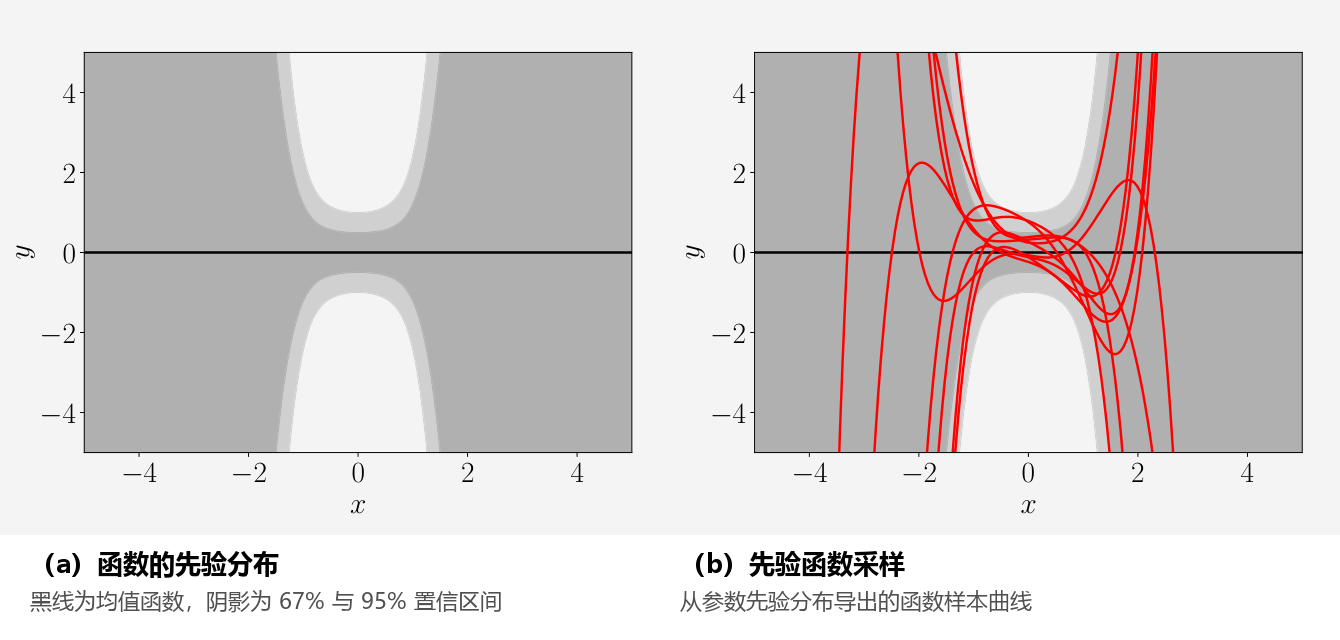
\includegraphics[width=0.92\textwidth,keepaspectratio]{docs/images/Figure9.9.png}
\caption*{图 9.9}
\end{figure}


迄今为止，我们考察了仅利用参数先验 $ p(\boldsymbol{\theta}) $ 计算预测分布。然而，当我们拥有了基于训练数据 $ \mathcal{X}, \mathcal{Y} $ 的参数后验分布后，预测和推断的原则与式 (9.37) 完全一致——我们只需将先验分布 $ p(\boldsymbol{\theta}) $ 替换为后验分布 $ p(\boldsymbol{\theta} \mid \mathcal{X}, \mathcal{Y}) $ 即可。在下文中，我们将先详细推导参数后验分布，然后再利用它进行预测。

\medskip\hrule\medskip

\section*{9.3.3 后验分布}
\addcontentsline{toc}{subsection}{9.3.3 后验分布}

给定由输入 $ \boldsymbol{x}_n \in \mathbb{R}^D $ 及对应观测值 $ y_n \in \mathbb{R} $（$ n = 1, \ldots, N $）组成的训练集，我们利用贝叶斯定理计算参数的后验分布：

\begin{equation}
p(\boldsymbol{\theta} \mid \mathcal{X}, \mathcal{Y}) = \frac{p(\mathcal{Y} \mid \mathcal{X}, \boldsymbol{\theta})p(\boldsymbol{\theta})}{p(\mathcal{Y} \mid \mathcal{X})}
\tag{9.41}
\end{equation}

其中 $ \mathcal{X} $ 为训练输入集合，$ \mathcal{Y} $ 为对应的训练目标集合。此外，$ p(\mathcal{Y} \mid \mathcal{X}, \boldsymbol{\theta}) $ 为似然函数，$ p(\boldsymbol{\theta}) $ 为参数先验，而

\begin{equation}
\begin{adjustbox}{max width=\linewidth}
p(\mathcal{Y} \mid \mathcal{X}) = \int p(\mathcal{Y} \mid \mathcal{X}, \boldsymbol{\theta})p(\boldsymbol{\theta}) \mathrm{d}\boldsymbol{\theta} = \mathbb{E}_{\boldsymbol{\theta}}\left[ p(\mathcal{Y} \mid \mathcal{X}, \boldsymbol{\theta}) \right]
\end{adjustbox}
\tag{9.42}
\end{equation}

为 \emph{边缘似然（marginal likelihood）} （亦称 \emph{模型证据（evidence）}）。它与模型参数 $ \boldsymbol{\theta} $ 无关，起到了归一化常数的作用，确保后验分布全域积分为 1。我们可以将边缘似然理解为似然在参数先验分布 $ p(\boldsymbol{\theta}) $ 下关于所有可能参数配置的期望平均。

\textbf{定理 9.1（参数后验分布）}。在模型 (9.35) 中，参数后验分布 (9.41) 可以闭式计算为高斯分布：

\begin{equation}
p(\boldsymbol{\theta} \mid \mathcal{X}, \mathcal{Y}) = \mathcal{N}\left(\boldsymbol{\theta} \mid \boldsymbol{m}_N, \boldsymbol{S}_N\right)
\tag{9.43a}
\end{equation}

\begin{equation}
\boldsymbol{S}_N = \left(\boldsymbol{S}_0^{-1} + \sigma^{-2}\boldsymbol{\Phi}^\top \boldsymbol{\Phi}\right)^{-1}
\tag{9.43b}
\end{equation}

\begin{equation}
\boldsymbol{m}_N = \boldsymbol{S}_N\left(\boldsymbol{S}_0^{-1}\boldsymbol{m}_0 + \sigma^{-2}\boldsymbol{\Phi}^\top \boldsymbol{y}\right)
\tag{9.43c}
\end{equation}

其中下标 $ N $ 表示训练集的样本容量。

*证明*。 根据贝叶斯定理，后验分布 $ p(\boldsymbol{\theta} \mid \mathcal{X}, \mathcal{Y}) $ 正比于似然函数与先验分布的乘积：

\begin{equation}
\textcn{后验：} \quad p(\boldsymbol{\theta} \mid \mathcal{X}, \mathcal{Y}) = \frac{p(\mathcal{Y} \mid \mathcal{X}, \boldsymbol{\theta})p(\boldsymbol{\theta})}{p(\mathcal{Y} \mid \mathcal{X})}
\tag{9.44a}
\end{equation}

\begin{equation}
\textcn{似然：} \quad p(\mathcal{Y} \mid \mathcal{X}, \boldsymbol{\theta}) = \mathcal{N}\left(\boldsymbol{y} \mid \boldsymbol{\Phi}\boldsymbol{\theta}, \sigma^2\boldsymbol{I}\right)
\tag{9.44b}
\end{equation}

\begin{equation}
\textcn{先验：} \quad p(\boldsymbol{\theta}) = \mathcal{N}\left(\boldsymbol{\theta} \mid \boldsymbol{m}_0, \boldsymbol{S}_0\right) .
\tag{9.44c}
\end{equation}

与其直接计算先验与似然的乘积，我们更方便将问题转换到对数空间中，并通过配方法（completing the squares）求解后验的均值与协方差。

对数先验与对数似然的和为：

\begin{equation}
\log \mathcal{N}\left(\boldsymbol{y} \mid \boldsymbol{\Phi}\boldsymbol{\theta}, \sigma^2\boldsymbol{I}\right) + \log \mathcal{N}\left(\boldsymbol{\theta} \mid \boldsymbol{m}_0, \boldsymbol{S}_0\right)
\tag{9.45a}
\end{equation}

\begin{equation}
\begin{adjustbox}{max width=\linewidth}
= -\frac{1}{2}\left[ \sigma^{-2}(\boldsymbol{y} - \boldsymbol{\Phi}\boldsymbol{\theta})^\top(\boldsymbol{y} - \boldsymbol{\Phi}\boldsymbol{\theta}) + (\boldsymbol{\theta} - \boldsymbol{m}_0)^\top \boldsymbol{S}_0^{-1}(\boldsymbol{\theta} - \boldsymbol{m}_0) \right] + \text{const}
\end{adjustbox}
\tag{9.45b}
\end{equation}

其中常数包含了与 $ \boldsymbol{\theta} $ 无关的所有项。在后文中我们将忽略该常数项。我们现在展开式 (9.45b)：

\begin{equation}
\begin{adjustbox}{max width=\linewidth}
-\frac{1}{2}\left[ \sigma^{-2}\boldsymbol{y}^\top \boldsymbol{y} - 2\sigma^{-2}\boldsymbol{y}^\top \boldsymbol{\Phi}\boldsymbol{\theta} + \boldsymbol{\theta}^\top \sigma^{-2}\boldsymbol{\Phi}^\top \boldsymbol{\Phi}\boldsymbol{\theta} + \boldsymbol{\theta}^\top \boldsymbol{S}_0^{-1}\boldsymbol{\theta} - 2\boldsymbol{m}_0^\top \boldsymbol{S}_0^{-1}\boldsymbol{\theta} + \boldsymbol{m}_0^\top \boldsymbol{S}_0^{-1}\boldsymbol{m}_0 \right]
\end{adjustbox}
\tag{9.46a}
\end{equation}

\begin{equation}
\begin{adjustbox}{max width=\linewidth}
= -\frac{1}{2}\left[ \boldsymbol{\theta}^\top\left(\sigma^{-2}\boldsymbol{\Phi}^\top \boldsymbol{\Phi} + \boldsymbol{S}_0^{-1}\right)\boldsymbol{\theta} - 2\left(\sigma^{-2}\boldsymbol{\Phi}^\top \boldsymbol{y} + \boldsymbol{S}_0^{-1}\boldsymbol{m}_0\right)^\top \boldsymbol{\theta} \right] + \text{const} .
\end{adjustbox}
\tag{9.46b}
\end{equation}

仔细审视式 (9.46b)，我们发现该式是关于 $ \boldsymbol{\theta} $ 的二次形式。未归一化的对数后验分布呈负二次型，这直接意味着后验分布必然是高斯分布，即：

\begin{equation}
\begin{adjustbox}{max width=\linewidth}
p(\boldsymbol{\theta} \mid \mathcal{X}, \mathcal{Y}) = \exp\left(\log p(\boldsymbol{\theta} \mid \mathcal{X}, \mathcal{Y})\right) \propto \exp\left(\log p(\mathcal{Y} \mid \mathcal{X}, \boldsymbol{\theta}) + \log p(\boldsymbol{\theta})\right)
\end{adjustbox}
\tag{9.47a}
\end{equation}

\begin{equation}
\begin{adjustbox}{max width=\linewidth}
\propto \exp\left( -\frac{1}{2}\left[ \boldsymbol{\theta}^\top\left(\sigma^{-2}\boldsymbol{\Phi}^\top \boldsymbol{\Phi} + \boldsymbol{S}_0^{-1}\right)\boldsymbol{\theta} - 2\left(\sigma^{-2}\boldsymbol{\Phi}^\top \boldsymbol{y} + \boldsymbol{S}_0^{-1}\boldsymbol{m}_0\right)^\top \boldsymbol{\theta} \right] \right) .
\end{adjustbox}
\tag{9.47b}
\end{equation}

接下来的任务是将这个（未归一化的）高斯分布整理成正比于 $ \mathcal{N}(\boldsymbol{\theta} \mid \boldsymbol{m}_N, \boldsymbol{S}_N) $ 的标准形式，即我们需要确定其均值 $ \boldsymbol{m}_N $ 和协方差矩阵 $ \boldsymbol{S}_N $。为此，我们使用配方法。标准目标对数后验形式为：

\begin{equation}
\begin{adjustbox}{max width=\linewidth}
\log \mathcal{N}\left(\boldsymbol{\theta} \mid \boldsymbol{m}_N, \boldsymbol{S}_N\right) = -\frac{1}{2}(\boldsymbol{\theta} - \boldsymbol{m}_N)^\top \boldsymbol{S}_N^{-1}(\boldsymbol{\theta} - \boldsymbol{m}_N) + \text{const}
\end{adjustbox}
\tag{9.48a}
\end{equation}

\begin{equation}
\begin{adjustbox}{max width=\linewidth}
= -\frac{1}{2}\left[ \boldsymbol{\theta}^\top \boldsymbol{S}_N^{-1}\boldsymbol{\theta} - 2\boldsymbol{m}_N^\top \boldsymbol{S}_N^{-1}\boldsymbol{\theta} + \boldsymbol{m}_N^\top \boldsymbol{S}_N^{-1}\boldsymbol{m}_N \right] .
\end{adjustbox}
\tag{9.48b}
\end{equation}

通过将式 (9.46b) 与式 (9.48b) 中关于 $ \boldsymbol{\theta} $ 的二次项与一次项进行系数匹配，我们解得：

\begin{equation}
\boldsymbol{S}_N^{-1} = \boldsymbol{\Phi}^\top \sigma^{-2}\boldsymbol{I}\boldsymbol{\Phi} + \boldsymbol{S}_0^{-1}
\tag{9.49a}
\end{equation}

\begin{equation}
\iff \boldsymbol{S}_N = \left(\sigma^{-2}\boldsymbol{\Phi}^\top \boldsymbol{\Phi} + \boldsymbol{S}_0^{-1}\right)^{-1}
\tag{9.49b}
\end{equation}

以及

\begin{equation}
\boldsymbol{m}_N^\top \boldsymbol{S}_N^{-1} = \left(\sigma^{-2}\boldsymbol{\Phi}^\top \boldsymbol{y} + \boldsymbol{S}_0^{-1}\boldsymbol{m}_0\right)^\top
\tag{9.50a}
\end{equation}

\begin{equation}
\iff \boldsymbol{m}_N = \boldsymbol{S}_N\left(\sigma^{-2}\boldsymbol{\Phi}^\top \boldsymbol{y} + \boldsymbol{S}_0^{-1}\boldsymbol{m}_0\right) .
\tag{9.50b}
\end{equation}

证毕。

\emph{备注} （配方法的通用方案） 。若给定形如

\begin{equation}
\boldsymbol{x}^\top \boldsymbol{A}\boldsymbol{x} - 2\boldsymbol{a}^\top \boldsymbol{x} + \text{const}_1
\tag{9.51}
\end{equation}

的方程（其中 $ \boldsymbol{A} $ 对称且正定），我们希望将其转化为完全平方式：

\begin{equation}
(\boldsymbol{x} - \boldsymbol{\mu})^\top \boldsymbol{\Sigma}(\boldsymbol{x} - \boldsymbol{\mu}) + \text{const}_2
\tag{9.52}
\end{equation}

我们可以通过令

\begin{equation}
\boldsymbol{\Sigma} := \boldsymbol{A}
\tag{9.53}
\end{equation}

\begin{equation}
\boldsymbol{\mu} := \boldsymbol{\Sigma}^{-1}\boldsymbol{a}
\tag{9.54}
\end{equation}

以及 $ \text{const}_2 = \text{const}_1 - \boldsymbol{\mu}^\top \boldsymbol{\Sigma}\boldsymbol{\mu} $ 即可达成。

我们可以看到，式 (9.47b) 中指数项内部的结构恰好具有式 (9.51) 的形式，其中：

\begin{equation}
\boldsymbol{A} := \sigma^{-2}\boldsymbol{\Phi}^\top \boldsymbol{\Phi} + \boldsymbol{S}_0^{-1}
\tag{9.55}
\end{equation}

\begin{equation}
\boldsymbol{a} := \sigma^{-2}\boldsymbol{\Phi}^\top \boldsymbol{y} + \boldsymbol{S}_0^{-1}\boldsymbol{m}_0 .
\tag{9.56}
\end{equation}

在复杂的多元推导中，将多项式方程整理成式 (9.51) 这种将二次项、线性项与常数项解耦的形式，能够极大简化配方求参数的过程。

\medskip\hrule\medskip

\section*{9.3.4 后验预测}
\addcontentsline{toc}{subsection}{9.3.4 后验预测}

在式 (9.37) 中，我们利用参数先验 $ p(\boldsymbol{\theta}) $ 计算了测试输入 $ \boldsymbol{x}_* $ 处的预测分布。原则上，使用参数后验 $ p(\boldsymbol{\theta} \mid \mathcal{X}, \mathcal{Y}) $ 进行预测并无本质不同，因为在我们的共轭模型中，先验和后验均为高斯分布（仅具有不同的均值和协方差参数）。因此，遵循与 9.3.2 节完全相同的推导逻辑，我们获得（后验）预测分布：

\begin{equation}
p(y_* \mid \mathcal{X}, \mathcal{Y}, \boldsymbol{x}_*) = \int p(y_* \mid \boldsymbol{x}_*, \boldsymbol{\theta})p(\boldsymbol{\theta} \mid \mathcal{X}, \mathcal{Y}) \mathrm{d}\boldsymbol{\theta}
\tag{9.57a}
\end{equation}

\begin{equation}
\begin{adjustbox}{max width=\linewidth}
= \int \mathcal{N}\left(y_* \mid \boldsymbol{\phi}^\top(\boldsymbol{x}_*)\boldsymbol{\theta}, \sigma^2\right) \mathcal{N}\left(\boldsymbol{\theta} \mid \boldsymbol{m}_N, \boldsymbol{S}_N\right) \mathrm{d}\boldsymbol{\theta}
\end{adjustbox}
\tag{9.57b}
\end{equation}

\begin{equation}
= \mathcal{N}\left(y_* \mid \boldsymbol{\phi}^\top(\boldsymbol{x}_*)\boldsymbol{m}_N, \boldsymbol{\phi}^\top(\boldsymbol{x}_*)\boldsymbol{S}_N\boldsymbol{\phi}(\boldsymbol{x}_*) + \sigma^2\right) .
\tag{9.57c}
\end{equation}

方差项中的 $ \boldsymbol{\phi}^\top(\boldsymbol{x}_*)\boldsymbol{S}_N\boldsymbol{\phi}(\boldsymbol{x}_*) $ 反映了在观测到训练数据后残余的参数后验不确定性。需要注意的是，$ \boldsymbol{S}_N $ 通过设计矩阵 $ \boldsymbol{\Phi} $ 依赖于训练输入；参见式 (9.43b)。预测均值 $ \boldsymbol{\phi}^\top(\boldsymbol{x}_*)\boldsymbol{m}_N $ 恰好与 MAP 估计值相吻合。

\emph{备注} （边缘似然与后验预测分布） 。通过替换式 (9.57a) 中的积分，后验预测分布可以等价地写为期望 $ \mathbb{E}_{\boldsymbol{\theta} \mid \mathcal{X}, \mathcal{Y}}\left[ p(y_* \mid \boldsymbol{x}_*, \boldsymbol{\theta}) \right] $，其中期望是关于参数后验分布 $ p(\boldsymbol{\theta} \mid \mathcal{X}, \mathcal{Y}) $ 计算的。将后验预测分布写成这种形式凸显了它与边缘似然 (9.42) 的高度相似性。边缘似然与后验预测分布之间的关键区别在于：(i) 边缘似然可以被视为对训练目标 $ \boldsymbol{y} $ 的预测，而非对测试目标 $ y_* $ 的预测；(ii) 边缘似然是关于参数先验求平均，而非关于参数后验求平均。

\emph{备注} （无噪声函数值的均值与方差） 。在很多应用中，我们感兴趣的并非带噪声观测值 $ y_* $ 的预测分布 $ p(y_* \mid \mathcal{X}, \mathcal{Y}, \boldsymbol{x}_*) $，而是希望获得（无噪声）底层函数值 $ f(\boldsymbol{x}_*) = \boldsymbol{\phi}^\top(\boldsymbol{x}_*)\boldsymbol{\theta} $ 的分布。利用均值和方差的性质，我们有：

\begin{equation}
\begin{adjustbox}{max width=\linewidth}
\mathbb{E}\left[ f(\boldsymbol{x}_*) \mid \mathcal{X}, \mathcal{Y} \right] = \mathbb{E}_{\boldsymbol{\theta}}\left[ \boldsymbol{\phi}^\top(\boldsymbol{x}_*)\boldsymbol{\theta} \mid \mathcal{X}, \mathcal{Y} \right] = \boldsymbol{\phi}^\top(\boldsymbol{x}_*)\mathbb{E}_{\boldsymbol{\theta}}[\boldsymbol{\theta} \mid \mathcal{X}, \mathcal{Y}] = \boldsymbol{\phi}^\top(\boldsymbol{x}_*)\boldsymbol{m}_N = \boldsymbol{m}_N^\top \boldsymbol{\phi}(\boldsymbol{x}_*)
\end{adjustbox}
\tag{9.58}
\end{equation}

\begin{equation}
\begin{adjustbox}{max width=\linewidth}
\mathbb{V}_{\boldsymbol{\theta}}\left[ f(\boldsymbol{x}_*) \mid \mathcal{X}, \mathcal{Y} \right] = \mathbb{V}_{\boldsymbol{\theta}}\left[ \boldsymbol{\phi}^\top(\boldsymbol{x}_*)\boldsymbol{\theta} \mid \mathcal{X}, \mathcal{Y} \right] = \boldsymbol{\phi}^\top(\boldsymbol{x}_*)\mathbb{V}_{\boldsymbol{\theta}}[\boldsymbol{\theta} \mid \mathcal{X}, \mathcal{Y}]\boldsymbol{\phi}(\boldsymbol{x}_*) = \boldsymbol{\phi}^\top(\boldsymbol{x}_*)\boldsymbol{S}_N\boldsymbol{\phi}(\boldsymbol{x}_*) .
\end{adjustbox}
\tag{9.59}
\end{equation}

我们看到，由于噪声均值为 0，预测均值与带噪声观测的均值完全相同；而预测方差仅相差 $ \sigma^2 $（测量噪声方差）：当我们预测带噪声的目标值时，需要计入 $ \sigma^2 $ 作为不确定性来源，但在预测无噪声真实函数值时则不需要该项。在此，唯一的残存不确定性源于参数后验分布。

\emph{备注} （函数上的分布） 。边缘化积分离出参数 $ \boldsymbol{\theta} $ 的操作诱导出了函数空间上的分布：如果我们从参数后验中抽取样本 $ \boldsymbol{\theta}_i \sim p(\boldsymbol{\theta} \mid \mathcal{X}, \mathcal{Y}) $，我们便获得了一个单项函数实现 $ \boldsymbol{\theta}_i^\top \boldsymbol{\phi}(\cdot) $。该函数分布的 \emph{均值函数（mean function）} （即所有期望函数值 $ \mathbb{E}_{\boldsymbol{\theta}}[f(\cdot) \mid \boldsymbol{\theta}, \mathcal{X}, \mathcal{Y}] $ 的集合）为 $ \boldsymbol{m}_N^\top \boldsymbol{\phi}(\cdot) $；其（边缘）方差（即函数 $ f(\cdot) $ 的方差）为 $ \boldsymbol{\phi}^\top(\cdot)\boldsymbol{S}_N\boldsymbol{\phi}(\cdot) $。

\begin{notebox}
\textbf{例 9.8（函数上的后验分布）}
\end{notebox}

\begin{notebox}
让我们重新考察 5 阶多项式的贝叶斯线性回归问题。参数先验取为 $ p(\boldsymbol{\theta}) = \mathcal{N}(\boldsymbol{0}, \frac{1}{4}\boldsymbol{I}) $。图 9.9 可视化了由该参数先验诱导的函数先验及先验样本函数。
\end{notebox}

\begin{notebox}
图 9.10 展示了通过贝叶斯线性回归获得的函数后验分布：

\begin{itemize}
\item 图 9.10(a) 展示了训练数据集；
\item 图 9.10(b) 展示了函数上的后验分布，包括通过极大似然估计（MLE）和最大后验估计（MAP）得到的函数。在贝叶斯线性回归设定下，MAP 估计得到的函数与后验均值函数完全重合；
\item 图 9.10(c) 展示了在该函数后验分布下抽取的若干合理函数实现（后验函数采样）。
\end{itemize}
\end{notebox}


\begin{figure}[H]
\centering
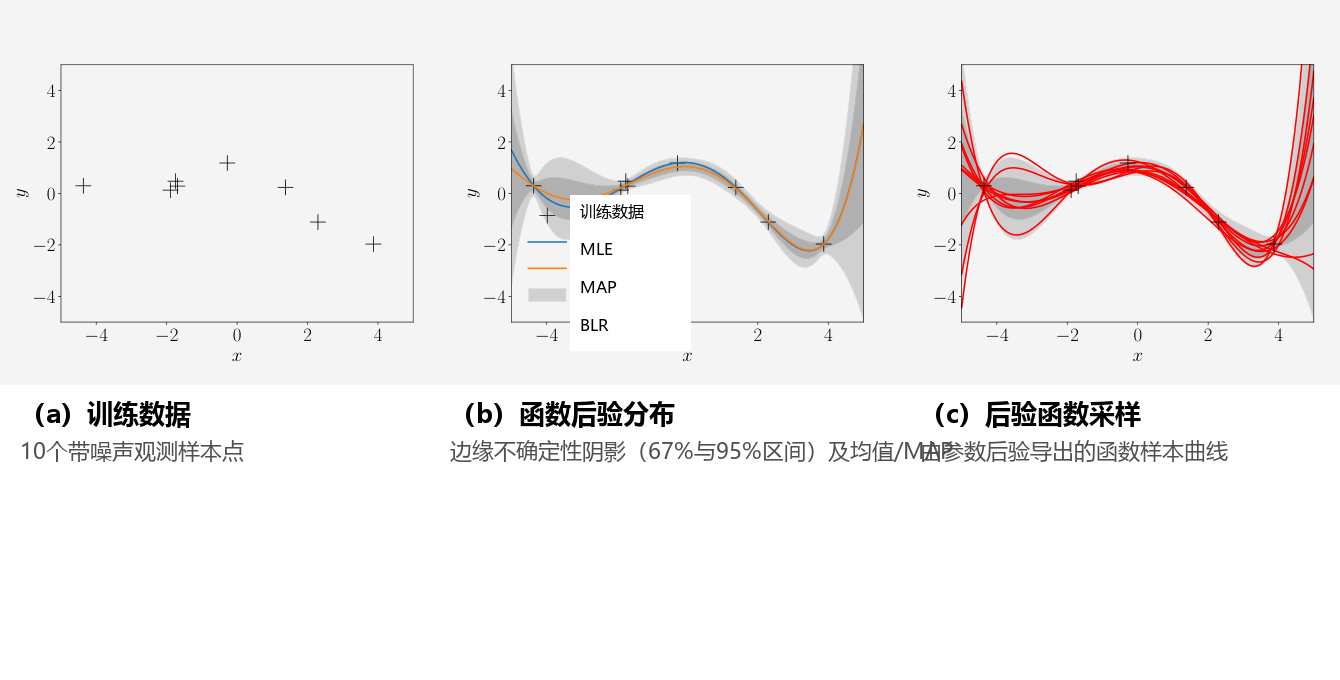
\includegraphics[width=0.92\textwidth,keepaspectratio]{docs/images/Figure9.10.png}
\caption*{图 9.10}
\end{figure}


图 9.11 展示了针对不同多项式阶数 $ M $ 由参数后验诱导出的函数后验分布：

\begin{itemize}
\item 左侧面板显示了极大似然函数 $ \boldsymbol{\theta}_{\text{ML}}^\top \boldsymbol{\phi}(\cdot) $、MAP 函数 $ \boldsymbol{\theta}_{\text{MAP}}^\top \boldsymbol{\phi}(\cdot) $（与后验均值函数相同），以及贝叶斯线性回归获得的 67\% 和 95\% 预测置信区间（阴影区域）；
\item 右侧面板显示了从函数后验中抽取的函数样本：在此我们从参数后验中采样参数 $ \boldsymbol{\theta}_i $，并计算函数曲线 $ \boldsymbol{\phi}^\top(x_*)\boldsymbol{\theta}_i $。
\end{itemize}


\begin{figure}[H]
\centering
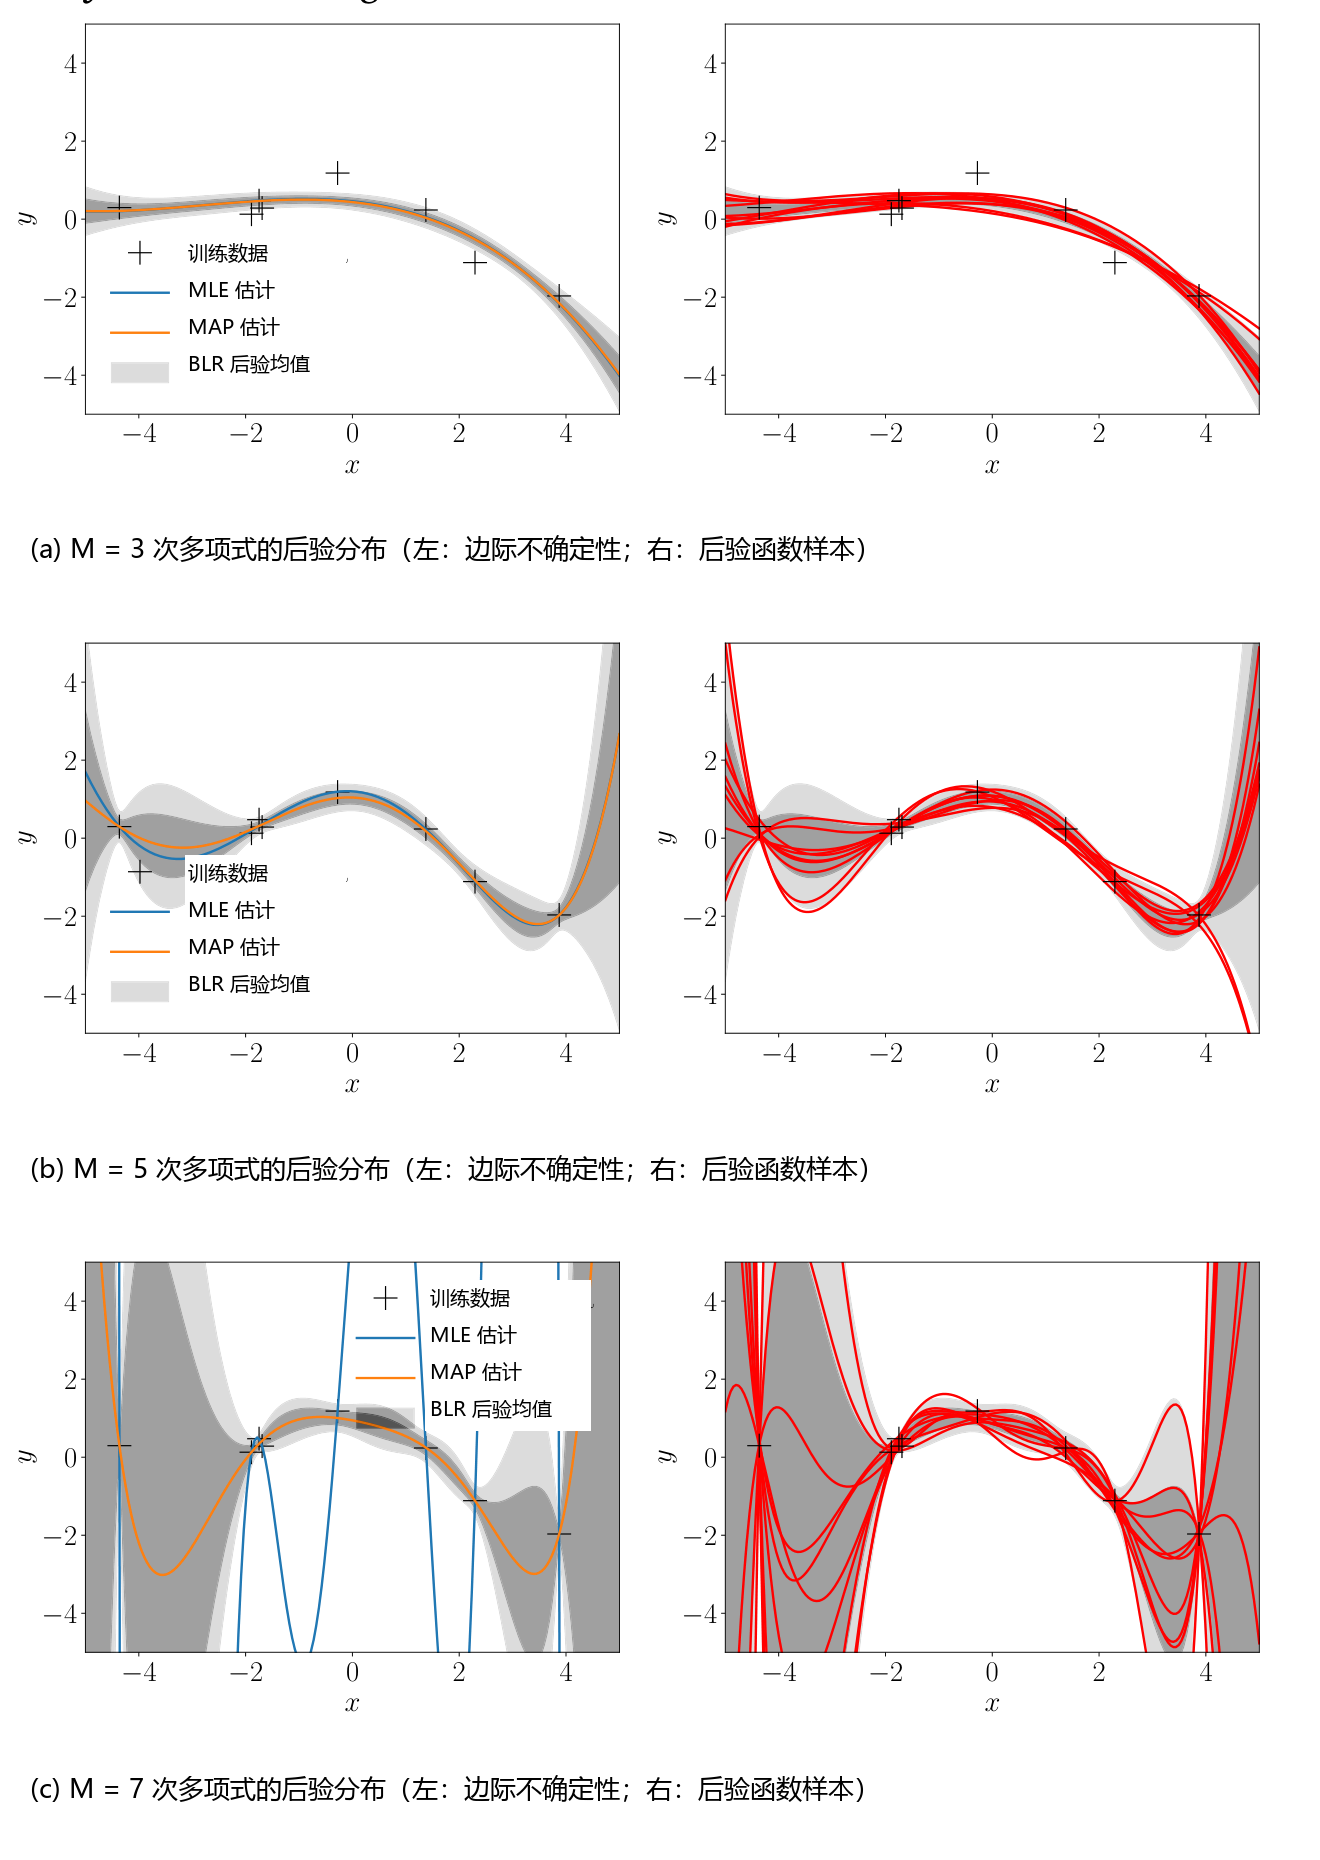
\includegraphics[width=0.95\textwidth,height=0.80\textheight,keepaspectratio]{docs/images/Figure9.11.png}
\caption*{图 9.11}
\end{figure}


对于低阶多项式，参数后验不允许参数发生剧烈变化：采样的函数曲线几乎完全重叠。当我们通过增加更多参数提高模型灵活性时（即采用更高阶的多项式），这些参数受到后验的约束变弱，采样的函数曲线在视觉上很容易彼此区分开来。我们也可以在对应的左侧面板中清楚地看到不确定性是如何显著增加的，尤其是在数据稀疏的边界区域。

尽管对于 7 阶多项式，MAP 估计给出了一个看起来尚可的拟合曲线，但贝叶斯线性回归模型额外告诉我们：在无数据覆盖的区域，后验不确定性极其巨大！当我们在决策系统（例如强化学习或机器人控制）中使用这些预测时，这种不确定性信息至关重要，因为在未知区域做出盲目自信的错误决策可能会带来灾难性的后果。

\medskip\hrule\medskip

\section*{9.3.5 计算边缘似然}
\addcontentsline{toc}{subsection}{9.3.5 计算边缘似然}

在 8.6.2 节中，我们强调了边缘似然对于贝叶斯模型选择的核心重要性。接下来，我们计算具有共轭高斯参数先验的贝叶斯线性回归的边缘似然，即本章一直探讨的设定。

简要回顾一下，我们考虑如下数据生成过程：

\begin{equation}
\boldsymbol{\theta} \sim \mathcal{N}\left(\boldsymbol{m}_0, \boldsymbol{S}_0\right)
\tag{9.60a}
\end{equation}

\begin{equation}
y_n \mid \boldsymbol{x}_n, \boldsymbol{\theta} \sim \mathcal{N}\left(\boldsymbol{x}_n^\top \boldsymbol{\theta}, \sigma^2\right) , \quad n = 1, \ldots, N .
\tag{9.60b}
\end{equation}

边缘似然由下式给出：

\begin{equation}
p(\mathcal{Y} \mid \mathcal{X}) = \int p(\mathcal{Y} \mid \mathcal{X}, \boldsymbol{\theta})p(\boldsymbol{\theta}) \mathrm{d}\boldsymbol{\theta}
\tag{9.61a}
\end{equation}

\begin{equation}
\begin{adjustbox}{max width=\linewidth}
= \int \mathcal{N}\left(\boldsymbol{y} \mid \boldsymbol{X}\boldsymbol{\theta}, \sigma^2\boldsymbol{I}\right) \mathcal{N}\left(\boldsymbol{\theta} \mid \boldsymbol{m}_0, \boldsymbol{S}_0\right) \mathrm{d}\boldsymbol{\theta}
\end{adjustbox}
\tag{9.61b}
\end{equation}

其中我们将模型参数 $ \boldsymbol{\theta} $ 积分离出。边缘似然可以理解为先验分布下的期望似然，即 $ \mathbb{E}_{\boldsymbol{\theta}}\left[ p(\mathcal{Y} \mid \mathcal{X}, \boldsymbol{\theta}) \right] $。我们分两步计算边缘似然：首先证明边缘似然（作为关于 $ \boldsymbol{y} $ 的分布）是高斯分布；其次计算该高斯分布的均值与协方差。

\begin{enumerate}
\item \textbf{边缘似然是高斯分布}：由 6.5.2 节可知，(i) 两个高斯随机变量密度的乘积是一个（未归一化的）高斯分布；(ii) 高斯随机变量的线性变换仍服从高斯分布。在式 (9.61b) 中，我们通过线性变换将 $ \mathcal{N}(\boldsymbol{y} \mid \boldsymbol{X}\boldsymbol{\theta}, \sigma^2\boldsymbol{I}) $ 化为关于 $ \boldsymbol{\theta} $ 的高斯形式 $ \mathcal{N}(\boldsymbol{\theta} \mid \boldsymbol{\mu}, \boldsymbol{\Sigma}) $。完成变换后，积分即可闭式求解。所得结果是两个高斯密度乘积的归一化常数，该常数本身关于 $ \boldsymbol{y} $ 具有高斯函数形状（参见式 (6.76)）。
\item \textbf{均值与协方差}：我们利用 6.4.4 节关于随机变量仿射变换均值和协方差的标准法则来求解边缘似然的矩。边缘似然的均值计算如下：
\end{enumerate}

\begin{equation}
\begin{adjustbox}{max width=\linewidth}
\mathbb{E}_{\boldsymbol{\theta}}[\mathcal{Y} \mid \mathcal{X}] = \mathbb{E}_{\boldsymbol{\theta}}[\boldsymbol{X}\boldsymbol{\theta} + \boldsymbol{\epsilon}] = \boldsymbol{X}\mathbb{E}_{\boldsymbol{\theta}}[\boldsymbol{\theta}] = \boldsymbol{X}\boldsymbol{m}_0 .
\end{adjustbox}
\tag{9.62}
\end{equation}

请注意，$ \boldsymbol{\epsilon} \sim \mathcal{N}(\boldsymbol{0}, \sigma^2\boldsymbol{I}) $ 是由独立同分布随机变量组成的噪声向量。协方差矩阵由下式给出：

\begin{equation}
\begin{adjustbox}{max width=\linewidth}
\text{Cov}_{\boldsymbol{\theta}}[\mathcal{Y} \mid \mathcal{X}] = \text{Cov}[\boldsymbol{X}\boldsymbol{\theta}] + \sigma^2\boldsymbol{I} = \boldsymbol{X} \text{Cov}_{\boldsymbol{\theta}}[\boldsymbol{\theta}] \boldsymbol{X}^\top + \sigma^2\boldsymbol{I}
\end{adjustbox}
\tag{9.63a}
\end{equation}

\begin{equation}
= \boldsymbol{X}\boldsymbol{S}_0\boldsymbol{X}^\top + \sigma^2\boldsymbol{I} .
\tag{9.63b}
\end{equation}

因此，边缘似然的解析闭式表达式为：

\begin{equation}
p(\mathcal{Y} \mid \mathcal{X}) = (2\pi)^{-\frac{N}{2}}\det\left(\boldsymbol{X}\boldsymbol{S}_0\boldsymbol{X}^\top + \sigma^2\boldsymbol{I}\right)^{-\frac{1}{2}}
\tag{9.64a}
\end{equation}

\begin{equation}
\begin{adjustbox}{max width=\linewidth}
\cdot \exp\left( -\frac{1}{2}(\boldsymbol{y} - \boldsymbol{X}\boldsymbol{m}_0)^\top\left(\boldsymbol{X}\boldsymbol{S}_0\boldsymbol{X}^\top + \sigma^2\boldsymbol{I}\right)^{-1}(\boldsymbol{y} - \boldsymbol{X}\boldsymbol{m}_0) \right)
\end{adjustbox}
\tag{9.64b}
\end{equation}

\begin{equation*}
= \mathcal{N}\left(\boldsymbol{y} \mid \boldsymbol{X}\boldsymbol{m}_0, \boldsymbol{X}\boldsymbol{S}_0\boldsymbol{X}^\top + \sigma^2\boldsymbol{I}\right) .
\end{equation*}

鉴于边缘似然与后验预测分布之间的紧密联系（参见本节前文关于边缘似然与后验预测分布的备注），边缘似然具有这种标准高斯函数形式是十分自然且符合直觉的。

\section*{9.4 极大似然作为正交投影}
\addcontentsline{toc}{section}{9.4 极大似然作为正交投影}
\label{sec:9.4}

在完成了大量复杂的代数推导以求取极大似然与 MAP 估计之后，我们现在为极大似然估计提供一个直观清晰的几何解释。

让我们首先考虑一个简单的线性回归设定：

\begin{equation}
y = x\theta + \epsilon , \quad \epsilon \sim \mathcal{N}\left(0, \sigma^2\right)
\tag{9.65}
\end{equation}

其中我们考虑通过原点的线性函数 $ f: \mathbb{R} \to \mathbb{R} $（为清晰起见，此处暂不引入特征映射）。参数 $ \theta $ 决定了直线的斜率。图 9.12(a) 展示了一个典型的一维数据集。


\begin{figure}[H]
\centering
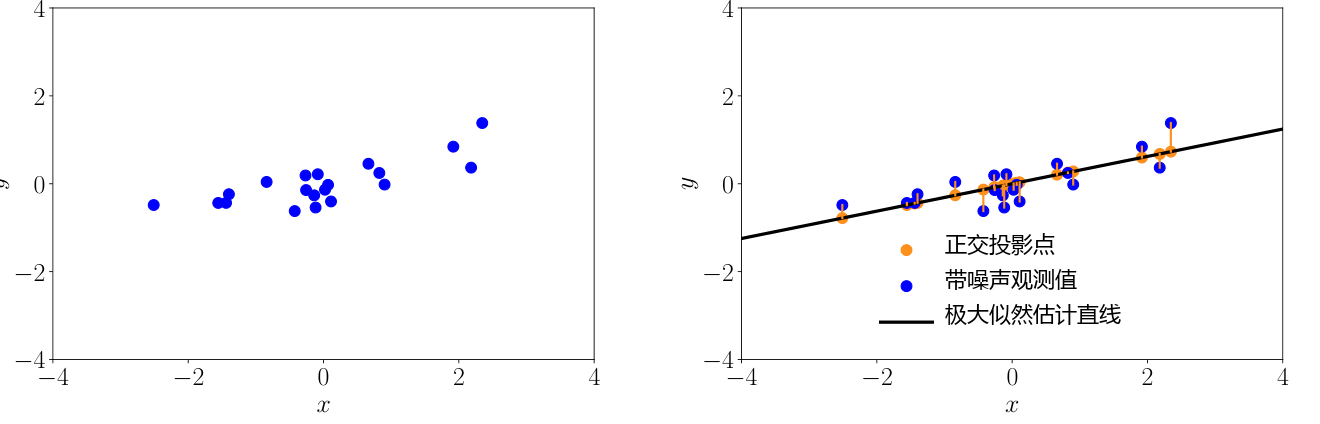
\includegraphics[width=0.92\textwidth,keepaspectratio]{docs/images/Figure9.12.png}
\caption*{图 9.12}
\end{figure}


给定训练数据集 $ \{(x_1, y_1), \ldots, (x_N, y_N)\} $，回顾 9.2.1 节的结果，斜率参数的极大似然估计量为：

\begin{equation}
\theta_{\text{ML}} = (\boldsymbol{X}^\top \boldsymbol{X})^{-1}\boldsymbol{X}^\top \boldsymbol{y} = \frac{\boldsymbol{X}^\top \boldsymbol{y}}{\boldsymbol{X}^\top \boldsymbol{X}} \in \mathbb{R}
\tag{9.66}
\end{equation}

其中 $ \boldsymbol{X} = [x_1, \ldots, x_N]^\top \in \mathbb{R}^N $，$ \boldsymbol{y} = [y_1, \ldots, y_N]^\top \in \mathbb{R}^N $。

这意味着，对于训练输入 $ \boldsymbol{X} $，我们获得训练目标的最佳（极大似然）重构为：

\begin{equation}
\boldsymbol{X}\theta_{\text{ML}} = \boldsymbol{X}\frac{\boldsymbol{X}^\top \boldsymbol{y}}{\boldsymbol{X}^\top \boldsymbol{X}} = \frac{\boldsymbol{X}\boldsymbol{X}^\top}{\boldsymbol{X}^\top \boldsymbol{X}}\boldsymbol{y}
\tag{9.67}
\end{equation}

即我们获得了 $ \boldsymbol{y} $ 与 $ \boldsymbol{X}\theta $ 之间具有最小二乘误差的最优近似。

由于我们寻找的是方程 $ \boldsymbol{y} = \boldsymbol{X}\theta $ 的解，我们可以将线性回归视为求解线性方程组的问题。因此，我们可以将第 2 章和第 3 章中讨论的线性代数与解析几何概念紧密联系起来。特别是，仔细观察式 (9.67)，我们发现式 (9.65) 中的极大似然估计量 $ \theta_{\text{ML}} $ 实际上是将观测目标向量 $ \boldsymbol{y} \in \mathbb{R}^N $ \emph{正交投影（orthogonal projection）} 到由输入向量 $ \boldsymbol{X} $ 所张成的一维子空间上！回顾 3.8 节关于正交投影的结论，我们可以识别出：

\begin{itemize}
\item $ \frac{\boldsymbol{X}\boldsymbol{X}^\top}{\boldsymbol{X}^\top \boldsymbol{X}} $ 是投影矩阵；
\item $ \theta_{\text{ML}} $ 是投影在由 $ \boldsymbol{X} $ 张成的 $ \mathbb{R}^N $ 的一维子空间中的坐标；
\item $ \boldsymbol{X}\theta_{\text{ML}} $ 则是 $ \boldsymbol{y} $ 在该子空间上的正交投影向量。
\end{itemize}

因此，极大似然解通过在由 $ \boldsymbol{X} $ 张成的子空间中寻找与对应观测值 $ \boldsymbol{y} $“最近”的向量，提供了几何上的最优解——这里的“最近”是指函数值 $ y_n $ 到 $ x_n\theta $ 的平方距离总和最小。这一几何最优性正是由正交投影实现的。图 9.12(b) 展示了带噪声观测值在使得原始数据集与其投影之间平方距离最小的子空间（固定 $ x $ 坐标）上的投影，这完全对应于极大似然解。

在具有向量值特征 $ \boldsymbol{\phi}(\boldsymbol{x}) \in \mathbb{R}^K $ 的一般线性回归情形中：

\begin{equation}
y = \boldsymbol{\phi}^\top(\boldsymbol{x})\boldsymbol{\theta} + \epsilon , \quad \epsilon \sim \mathcal{N}\left(0, \sigma^2\right)
\tag{9.68}
\end{equation}

我们同样可以将极大似然结果

\begin{equation}
\boldsymbol{y} \approx \boldsymbol{\Phi}\boldsymbol{\theta}_{\text{ML}}
\tag{9.69}
\end{equation}

\begin{equation}
\boldsymbol{\theta}_{\text{ML}} = (\boldsymbol{\Phi}^\top \boldsymbol{\Phi})^{-1}\boldsymbol{\Phi}^\top \boldsymbol{y}
\tag{9.70}
\end{equation}

解释为向 $ \mathbb{R}^N $ 中由特征矩阵 $ \boldsymbol{\Phi} $ 的列向量所张成的 $ K $ 维子空间上的正交投影；参见 3.8.2 节。

若用于构建特征矩阵 $ \boldsymbol{\Phi} $ 的特征基函数 $ \phi_k $ 是 \emph{标准正交（orthonormal）} 的（见 3.7 节），我们将得到一个特殊情形：$ \boldsymbol{\Phi} $ 的各列构成一组标准正交基（见 3.5 节），从而满足 $ \boldsymbol{\Phi}^\top \boldsymbol{\Phi} = \boldsymbol{I} $。此时投影矩阵简化为：

\begin{equation}
\begin{adjustbox}{max width=\linewidth}
\boldsymbol{\Phi}(\boldsymbol{\Phi}^\top \boldsymbol{\Phi})^{-1}\boldsymbol{\Phi}^\top \boldsymbol{y} = \boldsymbol{\Phi}\boldsymbol{\Phi}^\top \boldsymbol{y} = \left( \sum_{k=1}^K \boldsymbol{\phi}_k \boldsymbol{\phi}_k^\top \right) \boldsymbol{y}
\end{adjustbox}
\tag{9.71}
\end{equation}

此时不同特征之间的耦合完全消失，极大似然正交投影退化为 $ \boldsymbol{y} $ 向各个基向量 $ \boldsymbol{\phi}_k $（即 $ \boldsymbol{\Phi} $ 的各个列向量）上独立投影的简单线性叠加。信号处理中许多常用的基函数（如小波基和傅里叶基）都是正交基函数。当所选基不是正交基时，我们可以通过施密特正交化过程（Gram-Schmidt process，Strang, 2003）将一组线性无关的基函数转化为标准正交基。

\section*{9.5 延伸阅读}
\addcontentsline{toc}{section}{9.5 延伸阅读}
\label{sec:9.5}

在本章中，我们讨论了针对高斯似然与共轭高斯参数先验的线性回归模型，这使得闭式贝叶斯推断成为可能。然而，在某些实际应用中，我们可能需要选用完全不同的似然函数。例如：

\begin{itemize}
\item 在二元分类问题中，我们只能观测到两类离散标签，此时高斯似然显然是不适用的。相反，我们可以选择伯努利似然，它输出预测标签为 1（或 0）的概率。关于分类问题的深入介绍，读者可参阅 Barber (2012)、Bishop (2006) 以及 Murphy (2012) 的经典著作。
\item 另一个非高斯似然至关重要的领域是计数数据。计数是非负整数，在处理这类数据时，二项分布或泊松分布似然往往是比高斯分布好得多的选择。
\end{itemize}

所有这些例子都属于 \emph{广义线性模型（generalized linear models, GLM）} 的范畴。广义线性模型是线性回归的一种高度灵活的推广，它允许响应变量服从高斯分布以外的各类指数族误差分布。GLM 通过引入一个光滑且可逆的（可能非线性的）函数 $ \sigma(\cdot) $ 将线性模型与观测值联系起来，即：

\begin{equation*}
y = \sigma(f(\boldsymbol{x}))
\end{equation*}

其中 $ f(\boldsymbol{x}) = \boldsymbol{\theta}^\top \boldsymbol{\phi}(\boldsymbol{x}) $ 是式 (9.13) 中的线性回归模型。因此，我们可以从函数复合的角度将广义线性模型理解为 $ y = \sigma \circ f $，其中 $ f $ 是线性模型，而 $ \sigma $ 则是 \emph{激活函数（activation function）} 或 \emph{传递函数（transfer function）} ，其逆函数被称为 \emph{典型联系函数（canonical link function）} 。需要注意的是，尽管被称为“广义线性模型”，其输出 $ y $ 关于参数 $ \boldsymbol{\theta} $ 已不再呈线性。在 \emph{逻辑回归（logistic regression）} 中，我们选择 Logistic Sigmoid 函数：

\begin{equation*}
\sigma(f) = \frac{1}{1 + \exp(-f)} \in [0, 1]
\end{equation*}

它可以直接解释为伯努利随机变量 $ y \in \{0, 1\} $ 取值为 $ y = 1 $ 的后验概率。对于普通线性回归，其激活函数退化为简单的恒等映射。

从这个视角来看，广义线性模型显然也是（深度）前馈神经网络的基本构件：若我们考虑广义线性模型 $ \boldsymbol{y} = \sigma(\boldsymbol{A}\boldsymbol{x} + \boldsymbol{b}) $（其中 $ \boldsymbol{A} $ 为权重矩阵，$ \boldsymbol{b} $ 为偏置向量），我们便可将该广义线性模型识别为具有激活函数 $ \sigma(\cdot) $ 的单层神经网络。现在我们可以通过下式递归复合这些函数：

\begin{equation}
\boldsymbol{x}_{k+1} = f_k(\boldsymbol{x}_k) , \quad f_k(\boldsymbol{x}_k) = \sigma_k(\boldsymbol{A}_k\boldsymbol{x}_k + \boldsymbol{b}_k)
\tag{9.72}
\end{equation}

其中 $ k = 0, \ldots, K-1 $，$ \boldsymbol{x}_0 $ 为输入特征，$ \boldsymbol{x}_K = \boldsymbol{y} $ 为最终输出，从而 $ f_{K-1} \circ \cdots \circ f_0 $ 构成了一个 $ K $ 层的深度神经网络。因此，深度神经网络的基本构成单元正是式 (9.72) 中定义的广义线性模型。神经网络（Bishop, 1995; Goodfellow et al., 2016）比线性回归模型表达能力和拟合灵活性要强大得多；然而，其极大似然参数估计是一个非凸优化问题，而且在全贝叶斯框架下对其参数进行边缘化积分在解析上是不可行的。

我们之前简要指出过，参数上的分布会自然诱导出回归函数上的分布。 \emph{高斯过程（Gaussian process, GP）} （Rasmussen and Williams, 2006）正是一类以“函数上的分布”为核心概念的非参数回归模型。高斯过程不再在有限维参数上赋予先验分布，而是绕开参数的“弯路”，直接在无限维函数空间上定义先验与后验概率分布。为此，高斯过程巧妙地运用了 \emph{核技巧（kernel trick）} （Schölkopf and Smola, 2002），允许我们仅通过考察对应的输入 $ \boldsymbol{x}_i, \boldsymbol{x}_j $ 即可计算两个函数值 $ f(\boldsymbol{x}_i), f(\boldsymbol{x}_j) $ 之间的内积与协方差。高斯过程与贝叶斯线性回归、支持向量回归密切相关，同时也可以被严格等价解释为隐藏层单元数趋于无穷大的贝叶斯单隐层神经网络（Neal, 1996; Williams, 1997）。关于高斯过程的经典入门读物可参考 MacKay (1998) 以及 Rasmussen and Williams (2006)。

在本章的讨论中，我们重点关注了高斯参数先验，因为它们允许线性回归模型导出优雅的闭式贝叶斯推断。然而，即便在具有高斯似然的回归设定下，我们也可以根据先验假设选择非高斯先验。考虑输入 $ \boldsymbol{x} \in \mathbb{R}^D $ 且训练集规模极小（$ N \ll D $）的高维欠定场景。在这种情况下，回归方程严重欠定，我们可以选用能够强制产生 \emph{稀疏性（sparsity）} 的参数先验，即尽可能将大部分参数压缩归零的先验分布（从而实现 \emph{变量选择（variable selection）}）。这种先验比高斯先验提供了更强烈的正则化效应，往往能显著提高模型的预测精度与可解释性。 \emph{拉普拉斯先验（Laplace prior）} 是此类应用中最为常用的一种先验。在参数上引入拉普拉斯先验的线性回归模型，在数学上严格等价于带有 $ \ell_1 $ 正则化惩罚的线性回归（即 LASSO，Tibshirani, 1996）。拉普拉斯分布在零点处具有尖锐的峰值（其一阶导数在零点不连续），并且相比高斯分布将更大的概率质量高度集中在零点附近，从而极力促使模型参数精确为零。因此，最终保留下来的非零参数即为对回归问题真正显著的特征变量，这正是我们将其称为“变量选择”的原因。

\chapter{10 主成分分析降维}

直接处理高维数据（例如图像）会面临诸多现实困难：高维数据极难分析，直观解释十分困难，几何可视化几乎不可能，而且从工程实践的角度来看，存储高维数据向量的开销非常高昂（例如，一张 $ 640 \times 480 $ 像素的彩色图像就是近百万维空间中的一个数据点，因为每个像素对应红、绿、蓝三个颜色通道，即占用三个维度）。然而，高维数据通常具备许多我们可以利用的优良统计性质。例如，高维数据通常是 \emph{过完备（overcomplete）} 的，即许多维度是冗余的，可以由其他维度的某种组合来解释。此外，高维数据中各个维度之间往往存在显著的相关性，使得数据本身蕴含着内在的低维流形结构。 \emph{降维（dimensionality reduction）} 正是利用了这种内在结构与相关性，使我们能够使用更紧凑紧凑的数据表示，且理想情况下几乎不丢失关键信息。我们可以将降维视为一种数据压缩技术，类似于图像压缩领域的 JPEG 或音频压缩领域的 MP3。

在本章中，我们将深入讨论 \emph{主成分分析（principal component analysis, PCA）} ，这是一种用于线性降维的经典基础算法。PCA 最早由 Pearson (1901) 和 Hotelling (1933) 提出，距今已有百余年历史，至今仍是数据压缩与高维数据可视化中最常用的技术之一。它还被广泛用于发现高维数据中的简单模式、潜在因子（latent factors）和子空间结构。在信号处理领域，PCA 也被称为 \emph{K-L 变换（Karhunen-Loève transform）} 。在本章中，我们将从第一性原理出发推导 PCA，全面融合我们在本书第一部分掌握的基与基变换（2.6.1 和 2.7.2 节）、正交投影（3.8 节）、特征值与特征向量（4.2 节）、高斯分布（6.5 节）以及带约束连续优化（7.2 节）等数学概念。

降维通常利用了高维数据（如图像）的一个普遍特性：数据往往集中分布在一个低维子空间或其附近。图 10.1 给出了一个直观的二维示例。虽然图 10.1(a) 中的数据并没有严格落在一条直线上，但数据在 $ x_2 $ 方向上的方差非常微弱，因此我们可以将其近乎无损地表示为一条直线上的点；参见图 10.1(b)。为了描述图 10.1(b) 中的数据，仅需要单个 $ x_1 $ 坐标，此时数据实际上生活在 $ \mathbb{R}^2 $ 的一个一维子空间中。


\begin{figure}[H]
\centering
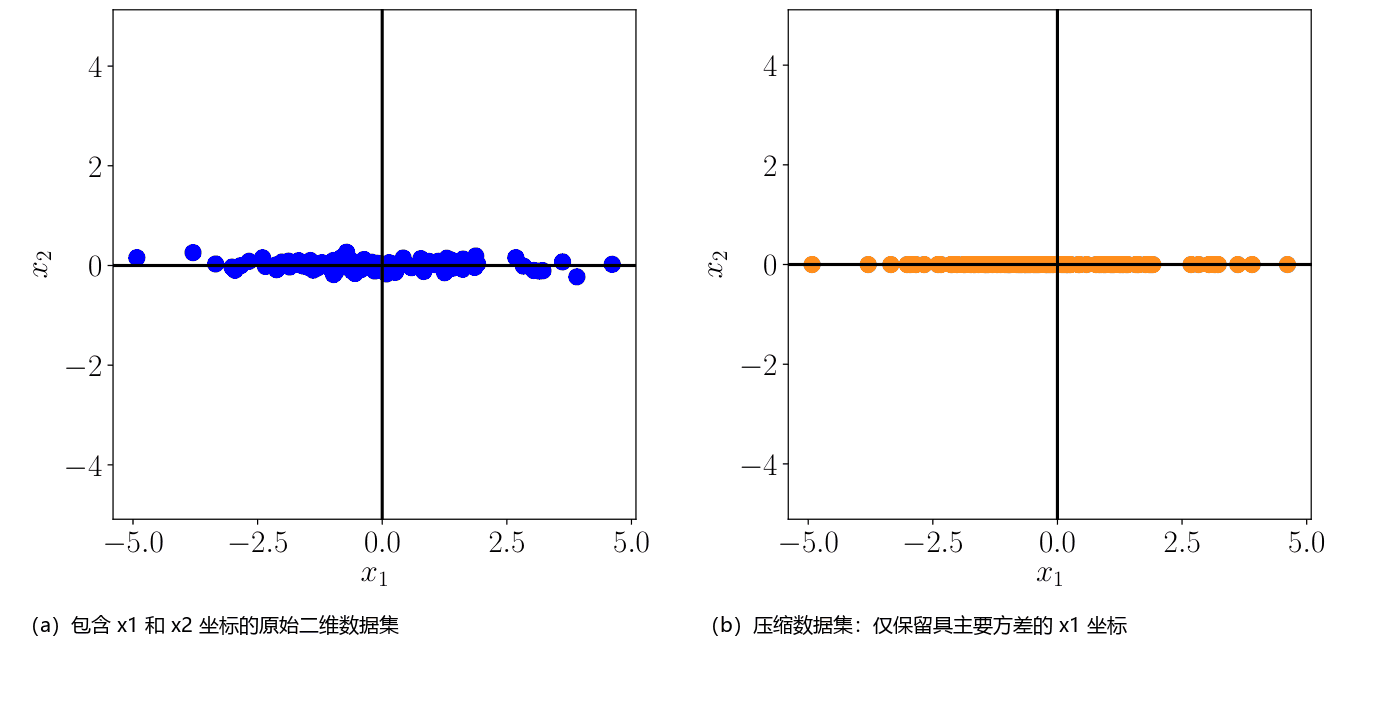
\includegraphics[width=0.92\textwidth,keepaspectratio]{docs/images/Figure10.1.png}
\caption*{图 10.1}
\end{figure}


在本章的后续部分：

\begin{itemize}
\item 10.1 节介绍降维的数学问题设置；
\item 10.2 节从“最大化投影方差”的经典视角推导 PCA；
\item 10.3 节从“最小化投影重构误差”的几何视角推导 PCA，并证明其与最大方差视角的严格等价性；
\item 10.4 节讨论特征向量计算与协方差矩阵的低秩近似；
\item 10.5 节讨论样本数小于数据维数时的高维 PCA 高效算法；
\item 10.6 节总结在实践中应用 PCA 的标准算法流程；
\item 10.7 节从概率图模型和高斯隐变量模型的视角探讨概率 PCA（PPCA）；
\item 10.8 节提供延伸阅读。
\end{itemize}

\section*{10.1 问题设置}
\addcontentsline{toc}{section}{10.1 问题设置}
\label{sec:10.1}

在 PCA 中，我们的目标是为高维数据点 $ \boldsymbol{x}_n $ 寻找投影点 $ \tilde{\boldsymbol{x}}_n $，使得这些投影点尽可能与原始数据点相似，但其内在维度显著降低。图 10.1 直观展示了这种降维效果。

更具体地说，我们考虑一个均值为零的独立同分布（i.i.d.）数据集 $ \mathcal{X} = \{\boldsymbol{x}_1, \ldots, \boldsymbol{x}_N\} $（$ \boldsymbol{x}_n \in \mathbb{R}^D $），其样本协方差矩阵（式 (6.42)）为：

\begin{equation}
\boldsymbol{S} = \frac{1}{N}\sum_{n=1}^N \boldsymbol{x}_n \boldsymbol{x}_n^\top .
\tag{10.1}
\end{equation}

此外，我们假设存在 $ \boldsymbol{x}_n $ 的低维压缩表示（称为 \emph{编码（code）}）：

\begin{equation}
\boldsymbol{z}_n = \boldsymbol{B}^\top \boldsymbol{x}_n \in \mathbb{R}^M
\tag{10.2}
\end{equation}

其中我们将投影矩阵定义为：

\begin{equation}
\boldsymbol{B} := [\boldsymbol{b}_1, \ldots, \boldsymbol{b}_M] \in \mathbb{R}^{D \times M} .
\tag{10.3}
\end{equation}

我们假设矩阵 $ \boldsymbol{B} $ 的列向量是标准正交的（定义 3.7），即当且仅当 $ i = j $ 时 $ \boldsymbol{b}_i^\top \boldsymbol{b}_j = 1 $，而当 $ i \neq j $ 时 $ \boldsymbol{b}_i^\top \boldsymbol{b}_j = 0 $。我们寻求一个 $ M $ 维子空间 $ U \subseteq \mathbb{R}^D $（$ \dim(U) = M < D $），并将数据投影到该子空间上。我们将投影后的数据记为 $ \tilde{\boldsymbol{x}}_n \in U $，其关于子空间 $ U $ 的基向量 $ \boldsymbol{b}_1, \ldots, \boldsymbol{b}_M $ 的坐标由 $ \boldsymbol{z}_n $ 给出。我们的目标是寻找投影点 $ \tilde{\boldsymbol{x}}_n \in \mathbb{R}^D $（或等价地寻找编码 $ \boldsymbol{z}_n $ 和基向量 $ \boldsymbol{b}_1, \ldots, \boldsymbol{b}_M $），使它们尽可能与原始数据 $ \boldsymbol{x}_n $ 相似，并最小化由压缩引起的信息损失。

\begin{notebox}
\textbf{例 10.1（坐标表示与编码）}
\end{notebox}

\begin{notebox}
考虑具有标准正交基 $ \boldsymbol{e}_1 = [1, 0]^\top, \boldsymbol{e}_2 = [0, 1]^\top $ 的向量空间 $ \mathbb{R}^2 $。由第 2 章可知，任意向量 $ \boldsymbol{x} \in \mathbb{R}^2 $ 均可表示为这些基向量的线性组合，例如：
\end{notebox}

\begin{notebox}
\begin{equation}
\begin{bmatrix} 5 \\ 3 \end{bmatrix} = 5\boldsymbol{e}_1 + 3\boldsymbol{e}_2 .
\tag{10.4}
\end{equation}
\end{notebox}

\begin{notebox}
然而，当我们考虑形如
\end{notebox}

\begin{notebox}
\begin{equation}
\tilde{\boldsymbol{x}} = \begin{bmatrix} 0 \\ z \end{bmatrix} \in \mathbb{R}^2 , \quad z \in \mathbb{R}
\tag{10.5}
\end{equation}
\end{notebox}

\begin{notebox}
的向量时，它们总是可以写为 $ 0\boldsymbol{e}_1 + z\boldsymbol{e}_2 $。为了完整表示这类向量，我们只需记录/存储 $ \tilde{\boldsymbol{x}} $ 关于基向量 $ \boldsymbol{e}_2 $ 的单个坐标（编码）$ z $ 即可。更准确地说，由所有这类 $ \tilde{\boldsymbol{x}} $ 构成的集合构成了 $ \mathbb{R}^2 $ 的一个向量子空间 $ U = \text{span}[\boldsymbol{e}_2] $，其维度为 $ \dim(U) = 1 $。
\end{notebox}

在 10.2 节中，我们将通过寻找能够保留尽可能多信息并最小化压缩损失的低维表示来推导 PCA。10.3 节给出了 PCA 的另一种等价几何推导视角，我们在其中最小化原始数据 $ \boldsymbol{x}_n $ 与其投影 $ \tilde{\boldsymbol{x}}_n $ 之间的平方重构误差 $ \|\boldsymbol{x}_n - \tilde{\boldsymbol{x}}_n\|^2 $。


\begin{figure}[H]
\centering
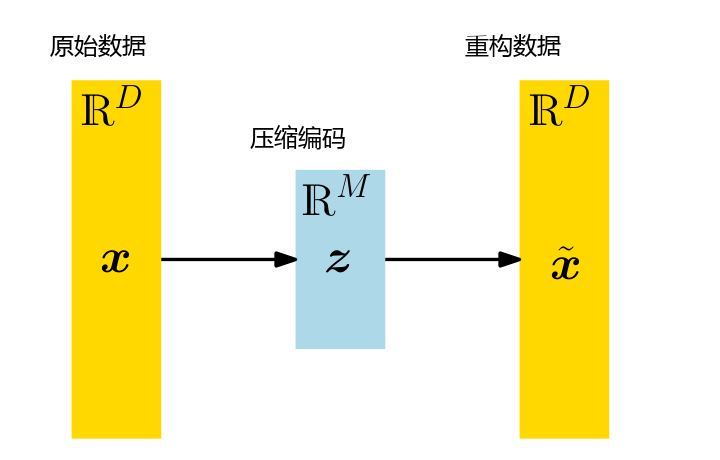
\includegraphics[width=0.92\textwidth,keepaspectratio]{docs/images/Figure10.2.png}
\caption*{图 10.2}
\end{figure}


图 10.2 展示了我们在 PCA 中考虑的系统架构：其中 $ \boldsymbol{z} $ 代表压缩数据 $ \tilde{\boldsymbol{x}} $ 的低维表示，起到了“信息瓶颈”（bottleneck）的作用，控制着 $ \boldsymbol{x} $ 与 $ \tilde{\boldsymbol{x}} $ 之间能够流动的信息量。在 PCA 中，我们考虑原始数据 $ \boldsymbol{x} $ 与其低维编码 $ \boldsymbol{z} $ 之间的线性关系，即对于适当的矩阵 $ \boldsymbol{B} $，有 $ \boldsymbol{z} = \boldsymbol{B}^\top \boldsymbol{x} $ 且 $ \tilde{\boldsymbol{x}} = \boldsymbol{B}\boldsymbol{z} $。基于将 PCA 视为数据压缩技术的直觉，我们可以将图 10.2 中的箭头解释为一对编码器（encoder）与解码器（decoder）操作：

\begin{itemize}
\item 由矩阵 $ \boldsymbol{B} $ 表示的线性映射可以被视为解码器，它将低维编码 $ \boldsymbol{z} \in \mathbb{R}^M $ 映射回原始数据空间 $ \mathbb{R}^D $；
\item 类似地，由矩阵 $ \boldsymbol{B}^\top $ 表示的线性映射可以被视为编码器，它将原始高维数据 $ \boldsymbol{x} $ 压缩编码为低维表示 $ \boldsymbol{z} $。
\end{itemize}

在贯穿本章的示例中，我们将使用 MNIST 手写数字数据集作为典型案例。该数据集包含 60,000 个手写数字 0 到 9 的样本。每个数字是一张 $ 28 \times 28 $ 像素的灰度图像，即包含 784 个像素点，因此我们可以将该数据集中的每张图像解释为一个高维向量 $ \boldsymbol{x} \in \mathbb{R}^{784} $。图 10.3 展示了该数据集中的部分手写数字图像。


\begin{figure}[H]
\centering

\includegraphics[width=0.92\textwidth,keepaspectratio]{docs/images/Figure10.3.png}
\caption*{图 10.3}
\end{figure}


\section*{10.2 最大方差视角}
\addcontentsline{toc}{section}{10.2 最大方差视角}
\label{sec:10.2}

图 10.1 展示了如何使用单个坐标来表示一个二维数据集。在图 10.1(b) 中，我们之所以选择忽略数据的 $ x_2 $ 坐标，是因为它包含的信息量很少，从而压缩后的数据与图 10.1(a) 中的原始数据非常相似。如果我们反过来选择忽略 $ x_1 $ 坐标，那么压缩后的数据将与原始数据大相径庭，数据中的大量关键信息都将丢失。

如果我们将数据中的“信息量”解释为数据集在空间中的“充盈程度”（space filling），那么我们可以通过考察数据的离散程度（分散程度）来量化数据所包含的信息。由 6.4.1 节可知， \emph{方差（variance）} 是衡量数据分散程度的绝佳指标，因此我们可以将 PCA 推导为一种通过最大化投影空间中低维数据方差来尽可能多地保留原始信息的降维算法。图 10.4 直观地说明了这一点。


\begin{figure}[H]
\centering
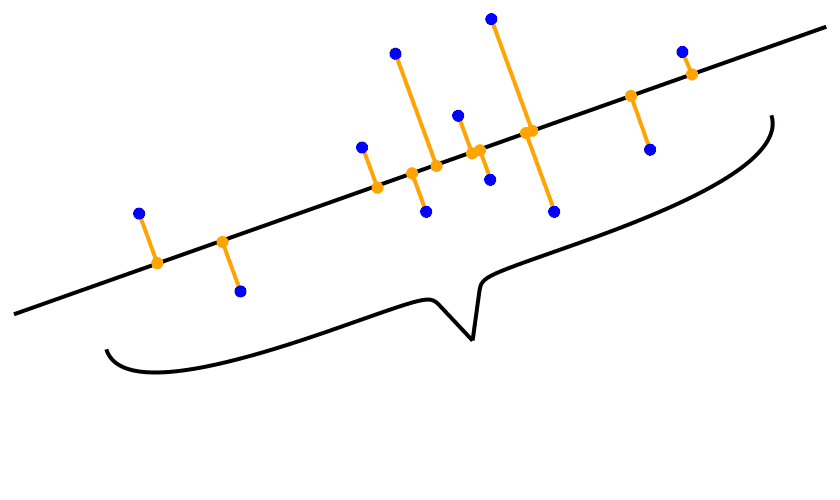
\includegraphics[width=0.92\textwidth,keepaspectratio]{docs/images/Figure10.4.png}
\caption*{图 10.4}
\end{figure}


结合 10.1 节讨论的问题设定，我们的目标是寻找一个矩阵 $ \boldsymbol{B} $（式 (10.3)），使得当我们将数据投影到由 $ \boldsymbol{B} $ 的列向量 $ \boldsymbol{b}_1, \ldots, \boldsymbol{b}_M $ 所张成的子空间时，能够保留尽可能多的信息。在数据压缩后保留最多信息，在统计学上等价于使低维编码捕获最大量的方差（Hotelling, 1933）。

\emph{备注} （中心化数据） 。对于式 (10.1) 中的样本协方差矩阵，我们假定数据是中心化的（均值为零）。我们可以不失一般性地做出这一假设：假设数据的真实样本均值为 $ \boldsymbol{\mu} $。利用我们在 6.4.4 节讨论的方差性质，我们有：

\begin{equation}
\begin{adjustbox}{max width=\linewidth}
\mathbb{V}_{\boldsymbol{z}}[\boldsymbol{z}] = \mathbb{V}_{\boldsymbol{x}}\left[\boldsymbol{B}^\top(\boldsymbol{x} - \boldsymbol{\mu})\right] = \mathbb{V}_{\boldsymbol{x}}\left[\boldsymbol{B}^\top\boldsymbol{x} - \boldsymbol{B}^\top\boldsymbol{\mu}\right] = \mathbb{V}_{\boldsymbol{x}}\left[\boldsymbol{B}^\top\boldsymbol{x}\right]
\end{adjustbox}
\tag{10.6}
\end{equation}

即低维编码的方差与原始数据的均值完全无关。因此，在本节的其余部分，我们不失一般性地假设数据的均值为 $ \boldsymbol{0} $。在此假设下，低维编码的均值同样为 $ \boldsymbol{0} $，因为

\begin{equation*}
\mathbb{E}_{\boldsymbol{z}}[\boldsymbol{z}] = \mathbb{E}_{\boldsymbol{x}}[\boldsymbol{B}^\top\boldsymbol{x}] = \boldsymbol{B}^\top\mathbb{E}_{\boldsymbol{x}}[\boldsymbol{x}] = \boldsymbol{0}
\end{equation*}

。

\medskip\hrule\medskip

\section*{10.2.1 最大方差方向}
\addcontentsline{toc}{subsection}{10.2.1 最大方差方向}

我们采用由浅入深的循序渐进法来最大化低维编码的方差。首先，我们寻求一个单一方向向量 $ \boldsymbol{b}_1 \in \mathbb{R}^D $，使得投影数据的方差最大化。这等价于最大化编码 $ \boldsymbol{z} \in \mathbb{R}^M $ 的第一个坐标 $ z_1 $ 的方差，即使得

\begin{equation}
V_1 := \mathbb{V}[z_1] = \frac{1}{N}\sum_{n=1}^N z_{1n}^2
\tag{10.7}
\end{equation}

最大化。这里我们利用了数据的独立同分布假设，并将 $ z_{1n} $ 定义为 $ \boldsymbol{x}_n \in \mathbb{R}^D $ 的低维表示 $ \boldsymbol{z}_n \in \mathbb{R}^M $ 的第一个分量。注意，$ \boldsymbol{z}_n $ 的第一个分量由下式给出：

\begin{equation}
z_{1n} = \boldsymbol{b}_1^\top \boldsymbol{x}_n
\tag{10.8}
\end{equation}

即它是 $ \boldsymbol{x}_n $ 在由 $ \boldsymbol{b}_1 $ 张成的一维子空间上的正交投影坐标（第 3.8 节）。将式 (10.8) 代入式 (10.7) 中，得到：

\begin{equation}
V_1 = \frac{1}{N}\sum_{n=1}^N \left(\boldsymbol{b}_1^\top \boldsymbol{x}_n\right)^2 = \frac{1}{N}\sum_{n=1}^N \boldsymbol{b}_1^\top \boldsymbol{x}_n \boldsymbol{x}_n^\top \boldsymbol{b}_1
\tag{10.9a}
\end{equation}

\begin{equation}
= \boldsymbol{b}_1^\top \left( \frac{1}{N}\sum_{n=1}^N \boldsymbol{x}_n \boldsymbol{x}_n^\top \right) \boldsymbol{b}_1 = \boldsymbol{b}_1^\top \boldsymbol{S}\boldsymbol{b}_1
\tag{10.9b}
\end{equation}

其中 $ \boldsymbol{S} $ 是式 (10.1) 中定义的样本协方差矩阵。在式 (10.9a) 中，我们利用了向量内积是对称的这一事实，即 $ \boldsymbol{b}_1^\top \boldsymbol{x}_n = \boldsymbol{x}_n^\top \boldsymbol{b}_1 $。

显然，若任意增大向量 $ \boldsymbol{b}_1 $ 的模长，方差 $ V_1 $ 也会随之增大（将 $ \boldsymbol{b}_1 $ 放大两倍将导致 $ V_1 $ 变为原来的四倍）。因此，为了使优化问题有意义，我们必须将解约束在单位球面 $ \|\boldsymbol{b}_1\|^2 = 1 $ 上。这导出了一个带约束的连续优化问题，我们在其中寻找数据方差最大的方向：

\begin{equation}
\max_{\boldsymbol{b}_1} \boldsymbol{b}_1^\top \boldsymbol{S}\boldsymbol{b}_1 \quad \text{subject to} \quad \|\boldsymbol{b}_1\|^2 = 1 .
\tag{10.10}
\end{equation}

遵循 7.2 节的拉格朗日乘子法，我们构建拉格朗日函数：

\begin{equation}
\mathcal{L}(\boldsymbol{b}_1, \lambda_1) = \boldsymbol{b}_1^\top \boldsymbol{S}\boldsymbol{b}_1 + \lambda_1\left(1 - \boldsymbol{b}_1^\top \boldsymbol{b}_1\right) .
\tag{10.11}
\end{equation}

$ \mathcal{L} $ 分别关于 $ \boldsymbol{b}_1 $ 和 $ \lambda_1 $ 的偏导数为：

\begin{equation}
\begin{adjustbox}{max width=\linewidth}
\frac{\partial \mathcal{L}}{\partial \boldsymbol{b}_1} = 2\boldsymbol{b}_1^\top \boldsymbol{S} - 2\lambda_1\boldsymbol{b}_1^\top , \qquad \frac{\partial \mathcal{L}}{\partial \lambda_1} = 1 - \boldsymbol{b}_1^\top \boldsymbol{b}_1 .
\end{adjustbox}
\tag{10.12}
\end{equation}

令这些偏导数为零，我们得到：

\begin{equation}
\boldsymbol{S}\boldsymbol{b}_1 = \lambda_1\boldsymbol{b}_1
\tag{10.13}
\end{equation}

\begin{equation}
\boldsymbol{b}_1^\top \boldsymbol{b}_1 = 1 .
\tag{10.14}
\end{equation}

与特征值分解的定义（4.4 节）对比，我们惊喜地发现：$ \boldsymbol{b}_1 $ 正是样本协方差矩阵 $ \boldsymbol{S} $ 的特征向量，而拉格朗日乘子 $ \lambda_1 $ 恰好扮演了对应特征值的角色！这一特征向量性质使我们能够重写方差目标函数：

\begin{equation}
V_1 = \boldsymbol{b}_1^\top \boldsymbol{S}\boldsymbol{b}_1 = \lambda_1 \boldsymbol{b}_1^\top \boldsymbol{b}_1 = \lambda_1
\tag{10.15}
\end{equation}

即数据投影到一维子空间后的方差，精确等于张成该子空间的基向量 $ \boldsymbol{b}_1 $ 所对应的特征值。因此，为了使投影后的方差最大化，我们应当选择对应于协方差矩阵 \textbf{最大特征值} 的特征向量。该特征向量被称为 \emph{第一主成分（first principal component）} 。数量 $ \sqrt{\lambda_1} $ 也被称为单位向量 $ \boldsymbol{b}_1 $ 的载荷（loading），表示主子空间 $ \text{span}[\boldsymbol{b}_1] $ 所解释的数据标准差。

我们可以通过将坐标 $ z_{1n} $ 映射回原始数据空间来确定主成分 $ \boldsymbol{b}_1 $ 的投影贡献，从而得到原始空间中的投影点：

\begin{equation}
\tilde{\boldsymbol{x}}_n = \boldsymbol{b}_1 z_{1n} = \boldsymbol{b}_1 \boldsymbol{b}_1^\top \boldsymbol{x}_n \in \mathbb{R}^D .
\tag{10.16}
\end{equation}

\emph{备注} 。尽管 $ \tilde{\boldsymbol{x}}_n $ 是一个 $ D $ 维向量，但它关于基向量 $ \boldsymbol{b}_1 \in \mathbb{R}^D $ 仅需要单个标量坐标 $ z_{1n} $ 即可完整表示。

\medskip\hrule\medskip

\section*{10.2.2 最大方差的 $ M $ 维子空间}
\addcontentsline{toc}{subsection}{10.2.2 最大方差的 $ M $ 维子空间}

假设我们已经求得了前 $ m-1 $ 个主成分，它们对应于协方差矩阵 $ \boldsymbol{S} $ 的前 $ m-1 $ 个最大特征值对应的特征向量 $ \boldsymbol{b}_1, \ldots, \boldsymbol{b}_{m-1} $。由于 $ \boldsymbol{S} $ 是对称矩阵，谱定理（定理 4.15）保证了我们可以利用这些特征向量构造 $ \mathbb{R}^D $ 的一个 $ (m-1) $ 维子空间的一组标准正交基。

一般地，第 $ m $ 个主成分可以通过从数据中剔除前 $ m-1 $ 个主成分的影响来寻找，从而尝试捕获剩余未被压缩的信息。由此我们构造剔除残差后的新数据矩阵：

\begin{equation}
\hat{\boldsymbol{X}} := \boldsymbol{X} - \sum_{i=1}^{m-1}\boldsymbol{b}_i \boldsymbol{b}_i^\top \boldsymbol{X} = \boldsymbol{X} - \boldsymbol{B}_{m-1}\boldsymbol{X}
\tag{10.17}
\end{equation}

其中 $ \boldsymbol{X} = [\boldsymbol{x}_1, \ldots, \boldsymbol{x}_N] \in \mathbb{R}^{D \times N} $ 将各个数据点作为列向量包含在内，$ \boldsymbol{B}_{m-1} := \sum_{i=1}^{m-1}\boldsymbol{b}_i \boldsymbol{b}_i^\top $ 是向由 $ \boldsymbol{b}_1, \ldots, \boldsymbol{b}_{m-1} $ 张成的子空间进行正交投影的投影矩阵。式 (10.17) 中的矩阵 $ \hat{\boldsymbol{X}} = [\hat{\boldsymbol{x}}_1, \ldots, \hat{\boldsymbol{x}}_N] \in \mathbb{R}^{D \times N} $ 包含了数据中尚未被前 $ m-1 $ 个主成分解释的信息。

\emph{备注} （符号约定） 。在本章中，我们不遵循将数据点 $ \boldsymbol{x}_1, \ldots, \boldsymbol{x}_N $ 作为数据矩阵各行的传统数据库习惯，而是将它们定义为 $ \boldsymbol{X} $ 的列向量。这意味着我们此处的数据矩阵 $ \boldsymbol{X} $ 是一个 $ D \times N $ 维矩阵，而非传统的 $ N \times D $ 矩阵。这一选择的原因在于，它能使代数运算极为流畅，无需反复转置矩阵或将向量重定义为左乘矩阵的行向量。

为了寻找第 $ m $ 个主成分，我们在约束条件 $ \|\boldsymbol{b}_m\|^2 = 1 $ 下最大化方差：

\begin{equation}
V_m = \mathbb{V}[z_m] = \frac{1}{N}\sum_{n=1}^N z_{mn}^2 = \frac{1}{N}\sum_{n=1}^N (\boldsymbol{b}_m^\top \hat{\boldsymbol{x}}_n)^2 = \boldsymbol{b}_m^\top \hat{\boldsymbol{S}}\boldsymbol{b}_m
\tag{10.18}
\end{equation}

其中 $ \hat{\boldsymbol{S}} $ 为变换后数据集 $ \hat{\boldsymbol{X}} $ 的样本协方差矩阵。与求解第一主成分类似，该带约束优化问题的最优解 $ \boldsymbol{b}_m $ 是 $ \hat{\boldsymbol{S}} $ 对应于其最大特征值的特征向量。

事实上，$ \boldsymbol{b}_m $ 同时也是原始协方差矩阵 $ \boldsymbol{S} $ 的特征向量！更一般地，$ \boldsymbol{S} $ 与 $ \hat{\boldsymbol{S}} $ 的特征向量集合是完全相同的。由于两者均为对称矩阵，由谱定理可知它们拥有共同的标准正交特征基。对于 $ \boldsymbol{S} $ 的任意特征向量 $ \boldsymbol{b}_i $（即 $ \boldsymbol{S}\boldsymbol{b}_i = \lambda_i \boldsymbol{b}_i $），我们有：

\begin{equation}
\begin{adjustbox}{max width=\linewidth}
\hat{\boldsymbol{S}}\boldsymbol{b}_i = \frac{1}{N}\hat{\boldsymbol{X}}\hat{\boldsymbol{X}}^\top \boldsymbol{b}_i = \frac{1}{N}(\boldsymbol{X} - \boldsymbol{B}_{m-1}\boldsymbol{X})(\boldsymbol{X} - \boldsymbol{B}_{m-1}\boldsymbol{X})^\top \boldsymbol{b}_i
\end{adjustbox}
\tag{10.19a}
\end{equation}

\begin{equation}
= \left(\boldsymbol{S} - \boldsymbol{S}\boldsymbol{B}_{m-1} - \boldsymbol{B}_{m-1}\boldsymbol{S} + \boldsymbol{B}_{m-1}\boldsymbol{S}\boldsymbol{B}_{m-1}\right)\boldsymbol{b}_i .
\tag{10.19b}
\end{equation}

我们分两种情形进行讨论：

\begin{enumerate}
\item 若 $ i \geqslant m $（即 $ \boldsymbol{b}_i $ 不在前 $ m-1 $ 个主成分中），则 $ \boldsymbol{b}_i $ 正交于前 $ m-1 $ 个主成分，故 $ \boldsymbol{B}_{m-1}\boldsymbol{b}_i = \boldsymbol{0} $；
\item 若 $ i < m $（即 $ \boldsymbol{b}_i $ 属于前 $ m-1 $ 个主成分之一），则 $ \boldsymbol{b}_i $ 属于投影子空间的基向量，故 $ \boldsymbol{B}_{m-1}\boldsymbol{b}_i = \boldsymbol{b}_i $。
\end{enumerate}

总结如下：

\begin{equation}
\boldsymbol{B}_{m-1}\boldsymbol{b}_i = \begin{cases} \boldsymbol{b}_i , & \textcn{若 } i < m , \\ \boldsymbol{0} , & \textcn{若 } i \geqslant m . \end{cases}
\tag{10.20}
\end{equation}

当 $ i \geqslant m $ 时，将式 (10.20) 代入式 (10.19b) 中，得到：

\begin{equation*}
\hat{\boldsymbol{S}}\boldsymbol{b}_i = (\boldsymbol{S} - \boldsymbol{B}_{m-1}\boldsymbol{S})\boldsymbol{b}_i = \boldsymbol{S}\boldsymbol{b}_i = \lambda_i \boldsymbol{b}_i
\end{equation*}

即 $ \boldsymbol{b}_i $ 也是 $ \hat{\boldsymbol{S}} $ 的特征值为 $ \lambda_i $ 的特征向量。特别地，对于 $ i = m $：

\begin{equation}
\hat{\boldsymbol{S}}\boldsymbol{b}_m = \boldsymbol{S}\boldsymbol{b}_m = \lambda_m \boldsymbol{b}_m .
\tag{10.21}
\end{equation}

式 (10.21) 揭示出：$ \lambda_m $ 既是 $ \hat{\boldsymbol{S}} $ 的最大特征值，也是 $ \boldsymbol{S} $ 的第 $ m $ 大特征值，两者的对应特征向量均为 $ \boldsymbol{b}_m $。

当 $ i < m $ 时，代入式 (10.19b) 得到：

\begin{equation}
\hat{\boldsymbol{S}}\boldsymbol{b}_i = (\boldsymbol{S} - \boldsymbol{S} - \boldsymbol{S} + \boldsymbol{S})\boldsymbol{b}_i = \boldsymbol{0} = 0\boldsymbol{b}_i .
\tag{10.22}
\end{equation}

这意味着 $ \boldsymbol{b}_1, \ldots, \boldsymbol{b}_{m-1} $ 也是 $ \hat{\boldsymbol{S}} $ 的特征向量，但对应的特征值退化为 0，即它们张成了 $ \hat{\boldsymbol{S}} $ 的零空间（null space）。

综上所述，$ \boldsymbol{S} $ 的每一个特征向量同样也是 $ \hat{\boldsymbol{S}} $ 的特征向量。由式 (10.21) 和 $ \boldsymbol{b}_m^\top \boldsymbol{b}_m = 1 $，数据投影到第 $ m $ 个主成分上的方差为：

\begin{equation}
V_m = \boldsymbol{b}_m^\top \boldsymbol{S}\boldsymbol{b}_m = \lambda_m \boldsymbol{b}_m^\top \boldsymbol{b}_m = \lambda_m .
\tag{10.23}
\end{equation}

这意味着：当数据投影到一个 $ M $ 维子空间时，所捕获的数据总方差恰好等于协方差矩阵对应的前 $ M $ 个特征向量的特征值之和！

\begin{notebox}
\textbf{例 10.2（MNIST 数字“8”的特征值）}
\end{notebox}

\begin{notebox}
取 MNIST 训练集中所有的手写数字“8”，计算其数据协方差矩阵的特征值。图 10.5(a) 展示了协方差矩阵中最大的 200 个特征值。我们清晰地看到，只有少数特征值显著大于零，其余特征值均迅速衰减趋向于零。因此，如图 10.5(b) 所示，当把数据投影到对应特征向量所张成的子空间时，绝大部分的数据方差仅由前少数几个主成分就足以充分捕获。
\end{notebox}


\begin{figure}[H]
\centering
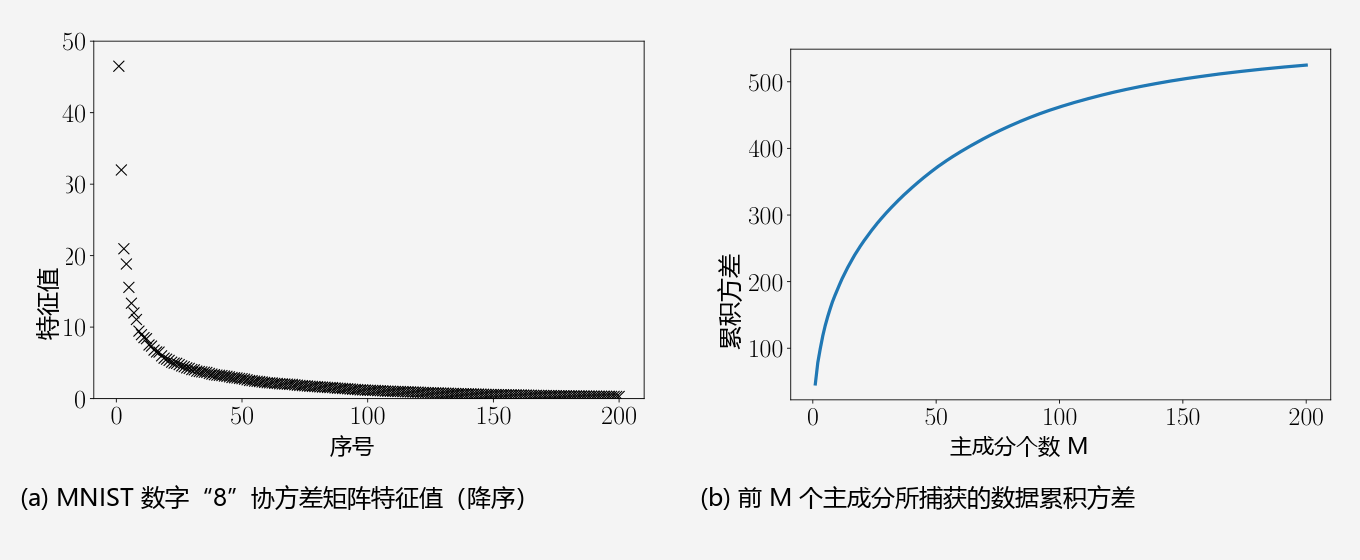
\includegraphics[width=0.92\textwidth,keepaspectratio]{docs/images/Figure10.5.png}
\caption*{图 10.5}
\end{figure}


总而言之，为了在 $ \mathbb{R}^D $ 中寻找一个保留尽可能多信息的 $ M $ 维子空间，PCA 明确告诉我们：\textbf{应当将投影矩阵 $ \boldsymbol{B} $（式 (10.3)）的列向量选取为数据协方差矩阵 $ \boldsymbol{S} $ 对应于 $ M $ 个最大特征值的特征向量}。

前 $ M $ 个主成分所能捕获的最大方差总量为：

\begin{equation}
V_M = \sum_{m=1}^M \lambda_m
\tag{10.24}
\end{equation}

其中 $ \lambda_m $ 为 $ \boldsymbol{S} $ 的前 $ M $ 个最大特征值。相应地，通过 PCA 压缩数据所损失的方差为剩余特征值的和：

\begin{equation}
J_M := \sum_{j=M+1}^D \lambda_j = V_D - V_M .
\tag{10.25}
\end{equation}

除了绝对方差指标，我们还常常定义相对捕获方差比率 $ \frac{V_M}{V_D} $（常称为 \emph{解释方差比（explained variance ratio）}），以及由压缩造成的相对方差损失率 $ 1 - \frac{V_M}{V_D} $。

\section*{10.3 投影视角}
\addcontentsline{toc}{section}{10.3 投影视角}
\label{sec:10.3}

在下文中，我们将把 PCA 推导为一种直接最小化平均重构误差的算法。这一视角使我们能够将 PCA 解释为实现了一个最优的线性自动编码器（linear auto-encoder）。在推导过程中，我们将深度运用第 2 章与第 3 章的几何工具。

在上一节中，我们通过最大化投影空间中的方差来保留尽可能多的信息，从而推导了 PCA。接下来，我们将考察原始数据点 $ \boldsymbol{x}_n $ 与其重构点 $ \tilde{\boldsymbol{x}}_n $ 之间的差值向量（位移向量），并通过最小化这一几何距离使得 $ \boldsymbol{x}_n $ 与 $ \tilde{\boldsymbol{x}}_n $ 尽可能接近。图 10.6 直观地展示了这一几何设定。


\begin{figure}[H]
\centering
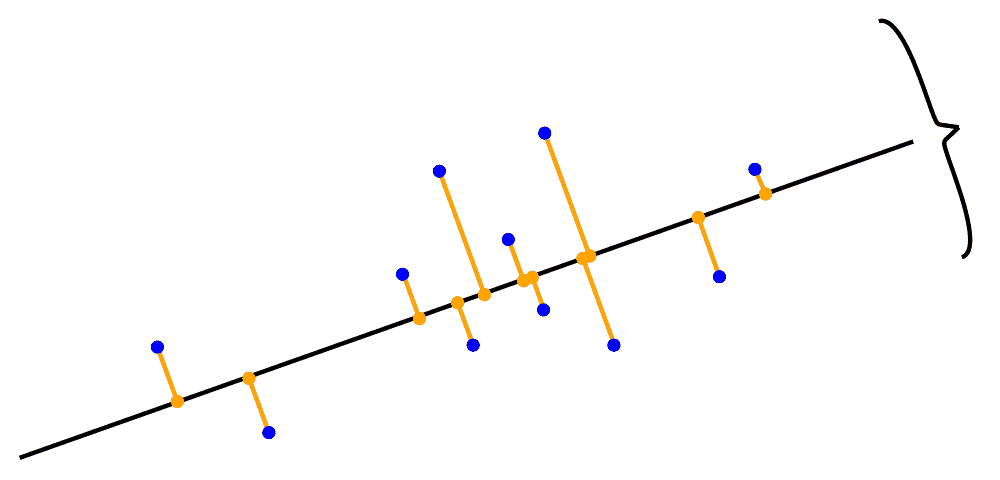
\includegraphics[width=0.92\textwidth,keepaspectratio]{docs/images/Figure10.6.png}
\caption*{图 10.6}
\end{figure}


\medskip\hrule\medskip

\section*{10.3.1 设定与目标}
\addcontentsline{toc}{subsection}{10.3.1 设定与目标}

假定 $ \mathcal{B} = (\boldsymbol{b}_1, \ldots, \boldsymbol{b}_D) $ 是 $ \mathbb{R}^D $ 的一组（有序）标准正交基（ONB），即当且仅当 $ i = j $ 时 $ \boldsymbol{b}_i^\top \boldsymbol{b}_j = 1 $，否则为 $ 0 $。

由 2.5 节可知，对于 $ \mathbb{R}^D $ 的任意基向量组 $ (\boldsymbol{b}_1, \ldots, \boldsymbol{b}_D) $，任意向量 $ \boldsymbol{x} \in \mathbb{R}^D $ 均可唯一表示为这些基向量的线性组合：

\begin{equation}
\boldsymbol{x} = \sum_{d=1}^D \zeta_d \boldsymbol{b}_d = \sum_{m=1}^M \zeta_m \boldsymbol{b}_m + \sum_{j=M+1}^D \zeta_j \boldsymbol{b}_j
\tag{10.26}
\end{equation}

其中 $ \zeta_d \in \mathbb{R} $ 为对应基向量下的坐标。

我们感兴趣的是在低维子空间 $ U \subseteq \mathbb{R}^D $（$ \dim(U) = M $）中寻找向量 $ \tilde{\boldsymbol{x}} \in \mathbb{R}^D $，使得

\begin{equation}
\tilde{\boldsymbol{x}} = \sum_{m=1}^M z_m \boldsymbol{b}_m \in U \subseteq \mathbb{R}^D
\tag{10.27}
\end{equation}

与 $ \boldsymbol{x} $ 尽可能相似。请注意，在此处我们暂且假设 $ \tilde{\boldsymbol{x}} $ 的坐标 $ z_m $ 与 $ \boldsymbol{x} $ 的坐标 $ \zeta_m $ 是未知的，不必事先假定它们完全相同。

接下来，我们正是利用 $ \tilde{\boldsymbol{x}} $ 的这种表示形式来求解最优坐标 $ \boldsymbol{z} $ 以及最优基向量 $ \boldsymbol{b}_1, \ldots, \boldsymbol{b}_M $，使得 $ \tilde{\boldsymbol{x}} $ 与原始数据点 $ \boldsymbol{x} $ 尽可能接近，即最小化欧几里得距离 $ \|\boldsymbol{x} - \tilde{\boldsymbol{x}}\| $。图 10.7 对这种几何配置进行了直观图解。


\begin{figure}[H]
\centering
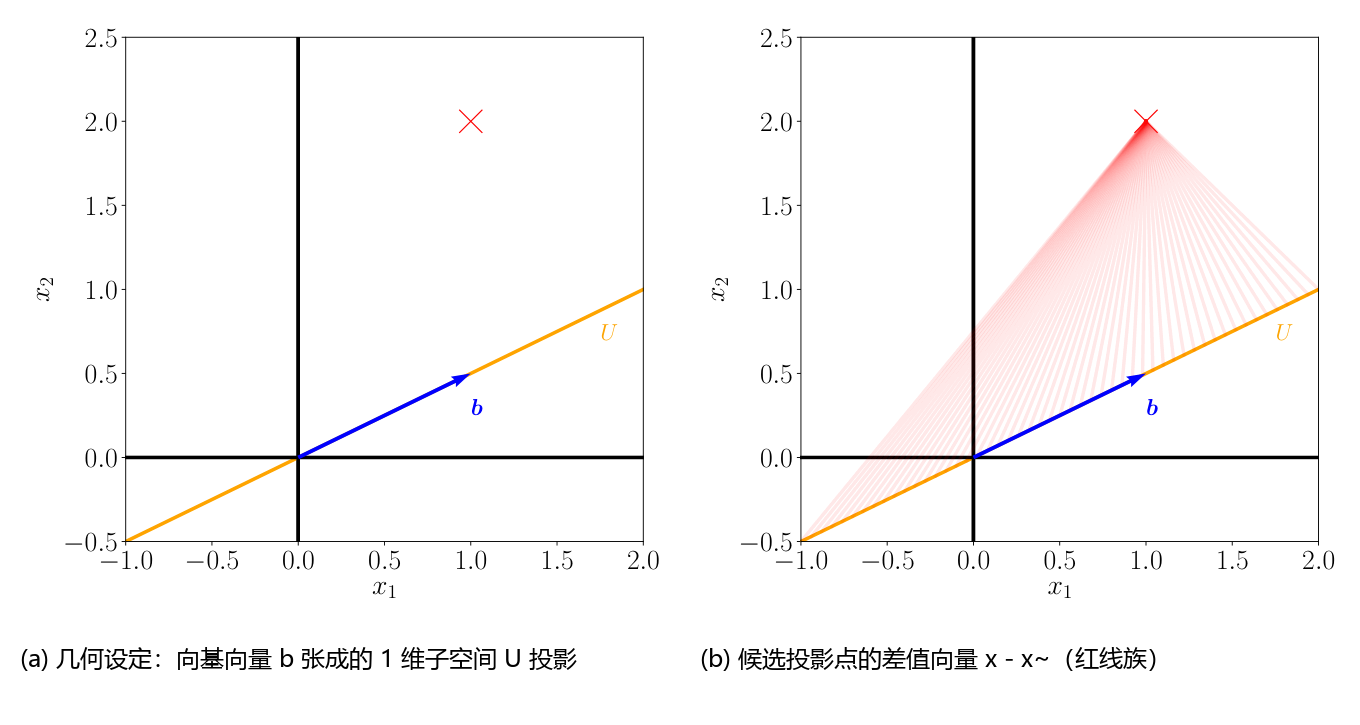
\includegraphics[width=0.92\textwidth,keepaspectratio]{docs/images/Figure10.7.png}
\caption*{图 10.7}
\end{figure}


不失一般性，我们假设数据集 $ \mathcal{X} = \{\boldsymbol{x}_1, \ldots, \boldsymbol{x}_N\} $（$ \boldsymbol{x}_n \in \mathbb{R}^D $）是中心化的，即样本均值为零 $ \mathbb{E}[\mathcal{X}] = \boldsymbol{0} $。若不假设零均值，推导出的数学结论完全一致，但公式符号会繁琐得多。

我们希望寻找 $ \mathcal{X} $ 向 $ \mathbb{R}^D $ 的 $ M $ 维低维子空间 $ U $（具有标准正交基 $ \boldsymbol{b}_1, \ldots, \boldsymbol{b}_M $）的最佳线性投影。我们称该子空间 $ U $ 为 \emph{主子空间（principal subspace）} 。数据点的投影点记为：

\begin{equation}
\tilde{\boldsymbol{x}}_n := \sum_{m=1}^M z_{mn} \boldsymbol{b}_m = \boldsymbol{B}\boldsymbol{z}_n \in \mathbb{R}^D
\tag{10.28}
\end{equation}

其中 $ \boldsymbol{z}_n := [z_{1n}, \ldots, z_{Mn}]^\top \in \mathbb{R}^M $ 是 $ \tilde{\boldsymbol{x}}_n $ 关于基 $ (\boldsymbol{b}_1, \ldots, \boldsymbol{b}_M) $ 的坐标向量。更具体地说，我们希望 $ \tilde{\boldsymbol{x}}_n $ 与 $ \boldsymbol{x}_n $ 尽可能接近。

我们采用欧几里得距离平方 $ \|\boldsymbol{x}_n - \tilde{\boldsymbol{x}}_n\|^2 $ 作为衡量两点差异的指标。因此，我们将目标函数定义为最小化平均平方欧几里得距离（即 \emph{重构误差（reconstruction error）} ，Pearson, 1901）：

\begin{equation}
J_M := \frac{1}{N}\sum_{n=1}^N \|\boldsymbol{x}_n - \tilde{\boldsymbol{x}}_n\|^2
\tag{10.29}
\end{equation}

其中下标 $ M $ 显式标明了数据所投影到的子空间维度。为了寻找最优线性投影，我们需要确定两组未知量：

\begin{enumerate}
\item 主子空间的一组标准正交基向量 $ \boldsymbol{b}_1, \ldots, \boldsymbol{b}_M $；
\item 投影点关于该组基的坐标 $ \boldsymbol{z}_n \in \mathbb{R}^M $（$ n = 1, \ldots, N $）。
\end{enumerate}

为此，我们采取两步优化策略：首先，在给定任意标准正交基 $ (\boldsymbol{b}_1, \ldots, \boldsymbol{b}_M) $ 的条件下优化坐标 $ \boldsymbol{z}_n $；其次，求解最优的标准正交基。

\medskip\hrule\medskip

\section*{10.3.2 寻找最优坐标}
\addcontentsline{toc}{subsection}{10.3.2 寻找最优坐标}

让我们首先固定一组标准正交基 $ (\boldsymbol{b}_1, \ldots, \boldsymbol{b}_M) $，求解使重构误差最小的最优坐标 $ z_{1n}, \ldots, z_{Mn} $（$ n = 1, \ldots, N $）。审视图 10.7(b)，当主子空间由单一向量 $ \boldsymbol{b} $ 张成时，从几何直观上寻找最优坐标 $ z $ 等价于在由 $ \boldsymbol{b} $ 张成的直线上寻找与 $ \boldsymbol{x} $ 距离最近的投影点 $ \tilde{\boldsymbol{x}} $。显然，这一最近点必然是 $ \boldsymbol{x} $ 在该直线上的 \textbf{正交投影点}。下面我们进行严谨证明。

利用链式求导法则，目标函数 $ J_M $ 关于坐标分量 $ z_{in} $（$ i = 1, \ldots, M $）的偏导数为：

\begin{equation}
\frac{\partial J_M}{\partial z_{in}} = \frac{\partial J_M}{\partial \tilde{\boldsymbol{x}}_n}\frac{\partial \tilde{\boldsymbol{x}}_n}{\partial z_{in}}
\tag{10.30a}
\end{equation}

其中

\begin{equation}
\frac{\partial J_M}{\partial \tilde{\boldsymbol{x}}_n} = -\frac{2}{N}(\boldsymbol{x}_n - \tilde{\boldsymbol{x}}_n)^\top \in \mathbb{R}^{1 \times D}
\tag{10.30b}
\end{equation}

以及由式 (10.28)：

\begin{equation}
\frac{\partial \tilde{\boldsymbol{x}}_n}{\partial z_{in}} = \frac{\partial}{\partial z_{in}}\left[ \sum_{m=1}^M z_{mn} \boldsymbol{b}_m \right] = \boldsymbol{b}_i .
\tag{10.30c}
\end{equation}

将式 (10.30b) 和 (10.30c) 结合：

\begin{equation}
\begin{adjustbox}{max width=\linewidth}
\frac{\partial J_M}{\partial z_{in}} = -\frac{2}{N}(\boldsymbol{x}_n - \tilde{\boldsymbol{x}}_n)^\top \boldsymbol{b}_i = -\frac{2}{N}\left( \boldsymbol{x}_n - \sum_{m=1}^M z_{mn} \boldsymbol{b}_m \right)^\top \boldsymbol{b}_i
\end{adjustbox}
\tag{10.31a}
\end{equation}

\begin{equation}
\overset{\text{ONB}}{=} -\frac{2}{N}\left(\boldsymbol{x}_n^\top \boldsymbol{b}_i - z_{in}\boldsymbol{b}_i^\top \boldsymbol{b}_i\right) = -\frac{2}{N}\left(\boldsymbol{x}_n^\top \boldsymbol{b}_i - z_{in}\right)
\tag{10.31b}
\end{equation}

这里我们利用了基向量的标准正交性（$ \boldsymbol{b}_m^\top \boldsymbol{b}_i = 0 $ 当 $ m \neq i $，以及 $ \boldsymbol{b}_i^\top \boldsymbol{b}_i = 1 $）。令该偏导数为 0，我们立即解得最优坐标：

\begin{equation}
z_{in} = \boldsymbol{x}_n^\top \boldsymbol{b}_i = \boldsymbol{b}_i^\top \boldsymbol{x}_n , \quad i = 1, \ldots, M , \quad n = 1, \ldots, N .
\tag{10.32}
\end{equation}

这意味着：投影点 $ \tilde{\boldsymbol{x}}_n $ 的最优坐标 $ z_{in} $ 恰好是原始数据点 $ \boldsymbol{x}_n $ 在由基向量 $ \boldsymbol{b}_i $ 张成的一维子空间上的正交投影坐标（参见第 3.8 节）。由此得出三条极其重要的核心结论：

\begin{enumerate}
\item \textbf{数据点 $ \boldsymbol{x}_n $ 的最优线性投影 $ \tilde{\boldsymbol{x}}_n $ 必然是正交投影}；
\item \textbf{$ \tilde{\boldsymbol{x}}_n $ 关于基 $ (\boldsymbol{b}_1, \ldots, \boldsymbol{b}_M) $ 的坐标，正是 $ \boldsymbol{x}_n $ 向主子空间作正交投影所得的坐标}；
\item \textbf{在均方误差目标 (10.29) 下，正交投影是数学上最优的线性降维映射}。
\end{enumerate}

图 10.8 展示了这一正交投影性质与距离极小值的几何对应关系。


\begin{figure}[H]
\centering
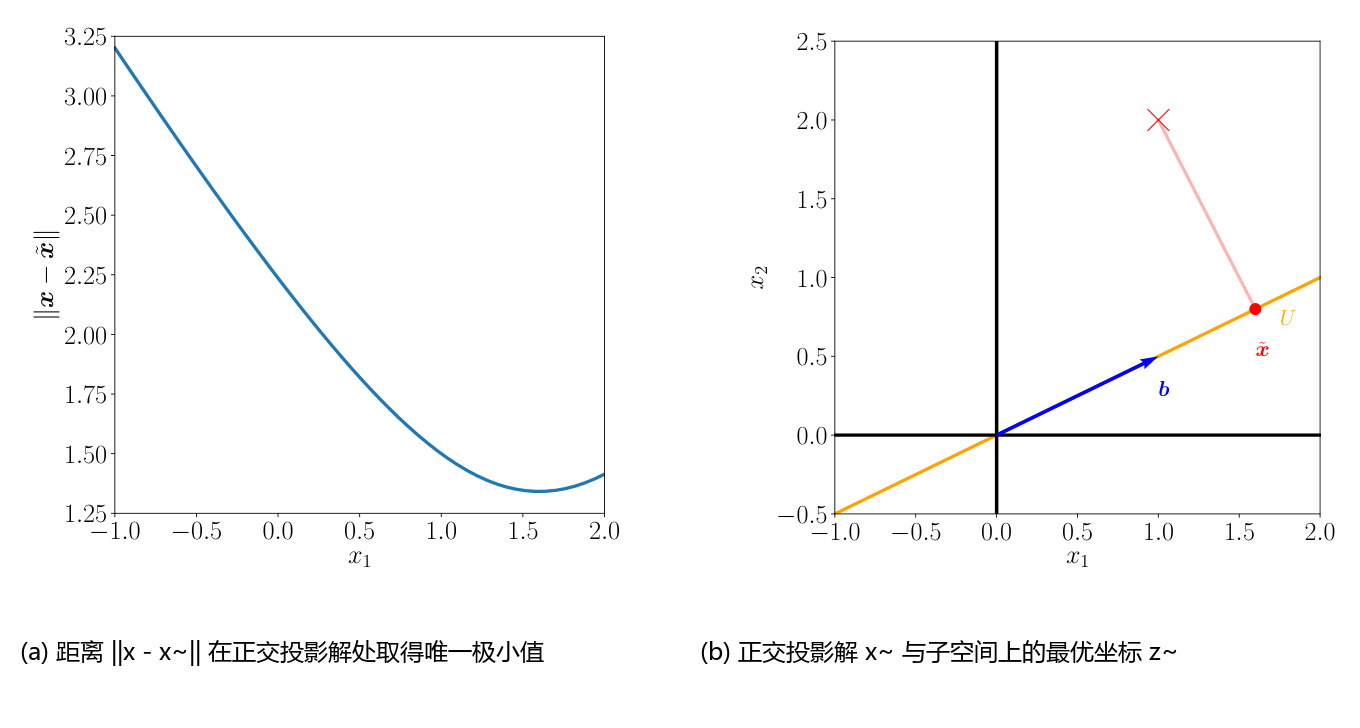
\includegraphics[width=0.92\textwidth,keepaspectratio]{docs/images/Figure10.8.png}
\caption*{图 10.8}
\end{figure}


\emph{备注} （标准正交基下的正交投影） 。简要回顾 3.8 节的正交投影理论：若 $ (\boldsymbol{b}_1, \ldots, \boldsymbol{b}_D) $ 为 $ \mathbb{R}^D $ 的标准正交基，则向由单个基向量 $ \boldsymbol{b}_j $ 张成的一维子空间的正交投影为：

\begin{equation}
\tilde{\boldsymbol{x}} = \boldsymbol{b}_j (\boldsymbol{b}_j^\top \boldsymbol{b}_j)^{-1}\boldsymbol{b}_j^\top \boldsymbol{x} = \boldsymbol{b}_j \boldsymbol{b}_j^\top \boldsymbol{x} \in \mathbb{R}^D
\tag{10.33}
\end{equation}

对应的坐标为标量 $ z_j = \boldsymbol{b}_j^\top \boldsymbol{x} $。更一般地，若向由标准正交基 $ \boldsymbol{b}_1, \ldots, \boldsymbol{b}_M $ 张成的 $ M $ 维子空间进行正交投影，投影点为：

\begin{equation}
\tilde{\boldsymbol{x}} = \boldsymbol{B}(\boldsymbol{B}^\top \boldsymbol{B})^{-1}\boldsymbol{B}^\top \boldsymbol{x} = \boldsymbol{B}\boldsymbol{B}^\top \boldsymbol{x}
\tag{10.34}
\end{equation}

其中利用了 $ \boldsymbol{B}^\top \boldsymbol{B} = \boldsymbol{I}_M $。该投影在有序基 $ (\boldsymbol{b}_1, \ldots, \boldsymbol{b}_M) $ 下的坐标向量为 $ \boldsymbol{z} := \boldsymbol{B}^\top \boldsymbol{x} \in \mathbb{R}^M $。

\medskip\hrule\medskip

\section*{10.3.3 寻找主子空间的基}
\addcontentsline{toc}{subsection}{10.3.3 寻找主子空间的基}

确定了给定基下的最优坐标后，接下来的核心任务是寻找最优的标准正交基向量 $ \boldsymbol{b}_1, \ldots, \boldsymbol{b}_M $。我们将已求得的最优坐标结果代入损失函数 (10.29) 中对其进行等价重构：

\begin{equation}
\tilde{\boldsymbol{x}}_n = \sum_{m=1}^M z_{mn}\boldsymbol{b}_m \overset{(10.32)}{=} \sum_{m=1}^M (\boldsymbol{x}_n^\top \boldsymbol{b}_m)\boldsymbol{b}_m .
\tag{10.35}
\end{equation}

利用内积的对称性，可得：

\begin{equation}
\tilde{\boldsymbol{x}}_n = \left( \sum_{m=1}^M \boldsymbol{b}_m \boldsymbol{b}_m^\top \right) \boldsymbol{x}_n .
\tag{10.36}
\end{equation}

由于完整的原始数据点 $ \boldsymbol{x}_n $ 可以按全部 $ D $ 个基向量精确展开：

\begin{equation}
\begin{adjustbox}{max width=\linewidth}
\boldsymbol{x}_n = \sum_{d=1}^D z_{dn}\boldsymbol{b}_d \overset{(10.32)}{=} \sum_{d=1}^D (\boldsymbol{x}_n^\top \boldsymbol{b}_d)\boldsymbol{b}_d = \left( \sum_{d=1}^D \boldsymbol{b}_d \boldsymbol{b}_d^\top \right) \boldsymbol{x}_n .
\end{adjustbox}
\tag{10.37a}
\end{equation}

\begin{equation}
= \left( \sum_{m=1}^M \boldsymbol{b}_m \boldsymbol{b}_m^\top \right) \boldsymbol{x}_n + \left( \sum_{j=M+1}^D \boldsymbol{b}_j \boldsymbol{b}_j^\top \right) \boldsymbol{x}_n .
\tag{10.37b}
\end{equation}

我们将包含 $ D $ 项的求和拆分为前 $ M $ 项与后 $ D-M $ 项。据此，原始数据点与重构点之间的差值向量（位移向量）精确为：

\begin{equation}
\boldsymbol{x}_n - \tilde{\boldsymbol{x}}_n = \left( \sum_{j=M+1}^D \boldsymbol{b}_j \boldsymbol{b}_j^\top \right) \boldsymbol{x}_n .
\tag{10.38a}
\end{equation}

\begin{equation}
= \sum_{j=M+1}^D (\boldsymbol{x}_n^\top \boldsymbol{b}_j)\boldsymbol{b}_j .
\tag{10.38b}
\end{equation}

这表明：\textbf{重构误差向量 $ \boldsymbol{x}_n - \tilde{\boldsymbol{x}}_n $ 恰好是数据点 $ \boldsymbol{x}_n $ 在主子空间的正交补空间 $ U^\perp $ 上的正交投影}！如图 10.9 所示，矩阵 $ \sum_{j=M+1}^D \boldsymbol{b}_j \boldsymbol{b}_j^\top $ 正是向正交补空间 $ U^\perp $ 投影的投影矩阵。


\begin{figure}[H]
\centering
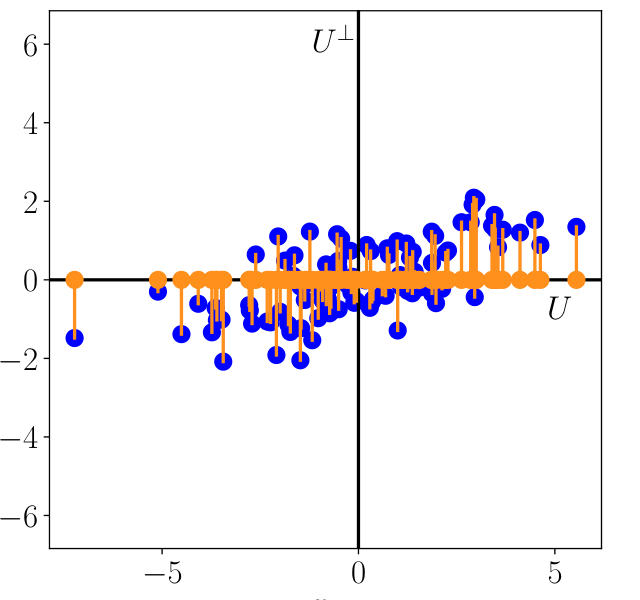
\includegraphics[width=0.92\textwidth,keepaspectratio]{docs/images/Figure10.9.png}
\caption*{图 10.9}
\end{figure}


\emph{备注} （低秩矩阵近似） 。在式 (10.38a) 中，我们看到投影到主子空间的投影矩阵由下式给出：

\begin{equation}
\sum_{m=1}^M \boldsymbol{b}_m \boldsymbol{b}_m^\top = \boldsymbol{B}\boldsymbol{B}^\top .
\tag{10.39}
\end{equation}

作为 $ M $ 个秩一外积矩阵的和，对称矩阵 $ \boldsymbol{B}\boldsymbol{B}^\top $ 的秩恰好为 $ M $。因此，平均平方重构误差可以等价写为：

\begin{equation}
\frac{1}{N}\sum_{n=1}^N \|\boldsymbol{x}_n - \tilde{\boldsymbol{x}}_n\|^2 = \frac{1}{N}\sum_{n=1}^N \|\boldsymbol{x}_n - \boldsymbol{B}\boldsymbol{B}^\top \boldsymbol{x}_n\|^2 .
\tag{10.40a}
\end{equation}

\begin{equation}
= \frac{1}{N}\sum_{n=1}^N \|(\boldsymbol{I} - \boldsymbol{B}\boldsymbol{B}^\top)\boldsymbol{x}_n\|^2 .
\tag{10.40b}
\end{equation}

寻找最小化重构误差的标准正交基向量 $ \boldsymbol{b}_1, \ldots, \boldsymbol{b}_M $，等价于寻找单位矩阵 $ \boldsymbol{I} $ 的最佳秩 $ M $ 近似矩阵 $ \boldsymbol{B}\boldsymbol{B}^\top $（见 4.6 节）。

现在我们将式 (10.38b) 代入重构误差函数 (10.29)：

\begin{equation}
J_M = \frac{1}{N}\sum_{n=1}^N \|\boldsymbol{x}_n - \tilde{\boldsymbol{x}}_n\|^2 = \frac{1}{N}\sum_{n=1}^N \left\| \sum_{j=M+1}^D (\boldsymbol{b}_j^\top \boldsymbol{x}_n)\boldsymbol{b}_j \right\|^2 .
\tag{10.41}
\end{equation}

由于基向量 $ \boldsymbol{b}_j $ 相互正交且模长为 1，展开范数平方可得：

\begin{equation}
J_M = \frac{1}{N}\sum_{n=1}^N \sum_{j=M+1}^D (\boldsymbol{b}_j^\top \boldsymbol{x}_n)^2 = \frac{1}{N}\sum_{n=1}^N \sum_{j=M+1}^D (\boldsymbol{b}_j^\top \boldsymbol{x}_n)(\boldsymbol{b}_j^\top \boldsymbol{x}_n)
\tag{10.42a}
\end{equation}

\begin{equation}
= \frac{1}{N}\sum_{n=1}^N \sum_{j=M+1}^D \boldsymbol{b}_j^\top \boldsymbol{x}_n \boldsymbol{x}_n^\top \boldsymbol{b}_j .
\tag{10.42b}
\end{equation}

交换求和次序，我们得到极为优雅的代数结果：

\begin{equation}
J_M = \sum_{j=M+1}^D \boldsymbol{b}_j^\top \left( \frac{1}{N}\sum_{n=1}^N \boldsymbol{x}_n \boldsymbol{x}_n^\top \right) \boldsymbol{b}_j = \sum_{j=M+1}^D \boldsymbol{b}_j^\top \boldsymbol{S}\boldsymbol{b}_j
\tag{10.43a}
\end{equation}

\begin{equation}
\begin{adjustbox}{max width=\linewidth}
= \sum_{j=M+1}^D \text{tr}\left(\boldsymbol{b}_j^\top \boldsymbol{S}\boldsymbol{b}_j\right) = \sum_{j=M+1}^D \text{tr}\left(\boldsymbol{S}\boldsymbol{b}_j \boldsymbol{b}_j^\top\right) = \text{tr}\left( \left( \sum_{j=M+1}^D \boldsymbol{b}_j \boldsymbol{b}_j^\top \right) \boldsymbol{S} \right)
\end{adjustbox}
\tag{10.43b}
\end{equation}

其中我们利用了迹算子 $ \text{tr}(\cdot) $ 的线性性质和循环置换不变性（式 (4.18)）。

式 (10.42a) 揭示了一个深刻的对偶事实：\textbf{平均平方重构误差等价于数据投影到主子空间的正交补空间后所保留的方差}！因此：

\begin{itemize}
\item \textbf{最小化平均平方重构误差}，等价于 \textbf{最小化被我们丢弃的子空间（正交补空间）中的数据方差}；
\item 等价地，这也等价于 \textbf{最大化保留在主子空间中的数据投影方差}！
\end{itemize}

这直接建立了投影视角与 10.2 节最大方差视角之间的严格数学等价性。根据 10.2 节的结论，在正交约束下，当选取的基向量为数据协方差矩阵的特征向量时，$ J_M $ 达到极值：

\begin{equation}
J_M = \sum_{j=M+1}^D \lambda_j .
\tag{10.44}
\end{equation}

为了使重构误差 $ J_M $ 达到全局最小，我们必须挑选数据协方差矩阵 \textbf{最小的 $ D-M $ 个特征值} 对应的特征向量作为正交补空间的基向量。这意味着：\textbf{主子空间的基向量 $ \boldsymbol{b}_1, \ldots, \boldsymbol{b}_M $ 必须精准选取为数据协方差矩阵对应于最大的 $ M $ 个特征值的特征向量}！

\begin{notebox}
\textbf{例 10.3（MNIST 数字低维嵌入）}
\end{notebox}

\begin{notebox}
图 10.10 可视化了 MNIST 数据集中手写数字“0”（蓝点）和“1”（橙点）嵌入到前两个主成分张成的二维主子空间中的结果。我们在图上高亮标出了部分数据点及其原始图像。该图揭示出：“0”与“1”在低维主子空间中展现出极其清晰的聚类分离界面，且数字“0”内部的形态方差显著大于数字“1”的内部方差。
\end{notebox}


\begin{figure}[H]
\centering
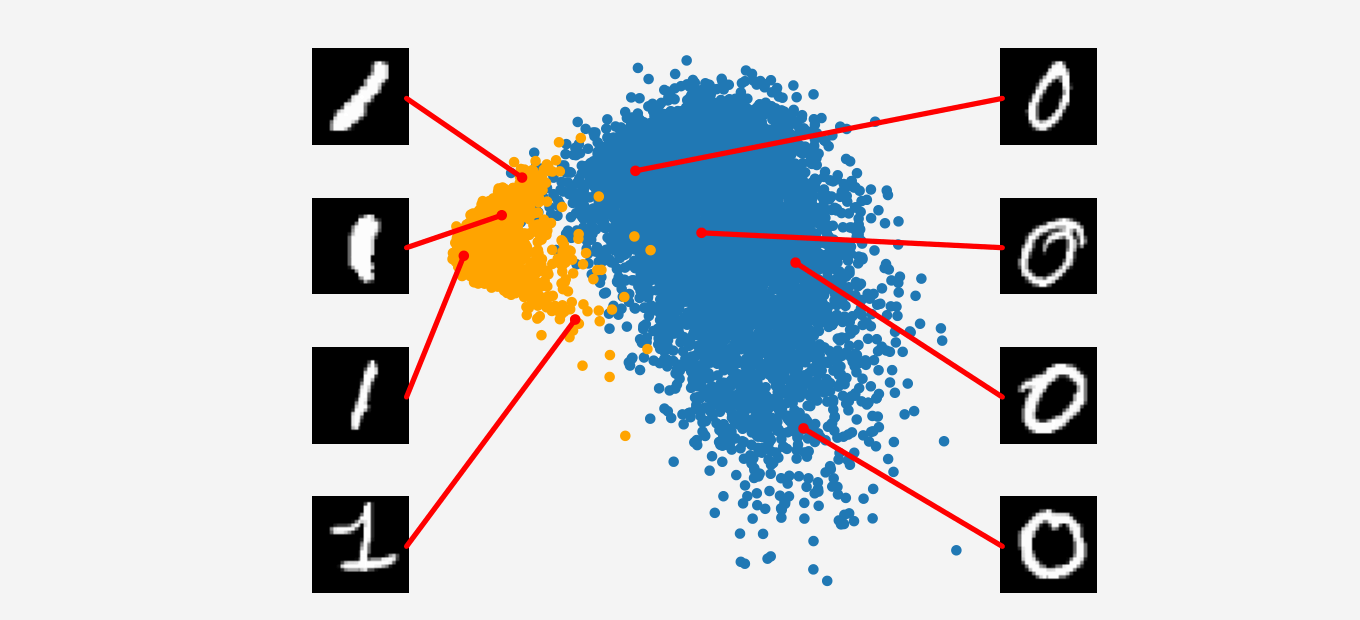
\includegraphics[width=0.92\textwidth,keepaspectratio]{docs/images/Figure10.10.png}
\caption*{图 10.10}
\end{figure}


\section*{10.4 特征向量计算与低秩近似}
\addcontentsline{toc}{section}{10.4 特征向量计算与低秩近似}
\label{sec:10.4}

在前面的章节中，我们证明了主子空间的最优基向量对应于样本协方差矩阵的最大特征值对应的特征向量：

\begin{equation}
\boldsymbol{S} = \frac{1}{N}\sum_{n=1}^N \boldsymbol{x}_n \boldsymbol{x}_n^\top = \frac{1}{N}\boldsymbol{X}\boldsymbol{X}^\top
\tag{10.45}
\end{equation}

\begin{equation}
\boldsymbol{X} = [\boldsymbol{x}_1, \ldots, \boldsymbol{x}_N] \in \mathbb{R}^{D \times N} .
\tag{10.46}
\end{equation}

需要再次提醒的是，此处的 $ \boldsymbol{X} $ 是一个 $ D \times N $ 维矩阵，即传统数据库数据矩阵的转置。为了求解 $ \boldsymbol{S} $ 的特征值及其对应的特征向量，我们可以采取两条互补的数学路径：

\begin{enumerate}
\item \textbf{直接特征值分解}：按照 4.2 节的方法，直接计算对称矩阵 $ \boldsymbol{S} $ 的特征值分解；
\item \textbf{奇异值分解（SVD）}：按照 4.5 节的方法，对中心化数据矩阵 $ \boldsymbol{X} $ 进行奇异值分解。由于 $ \boldsymbol{S} $ 是对称的且在常数因子意义下分解为 $ \boldsymbol{X}\boldsymbol{X}^\top $，$ \boldsymbol{S} $ 的特征值恰好等于 $ \boldsymbol{X} $ 的奇异值的平方除以 $ N $。
\end{enumerate}

更具体地说，矩阵 $ \boldsymbol{X} $ 的奇异值分解为：

\begin{equation}
\boldsymbol{X} = \boldsymbol{U}\boldsymbol{\Sigma}\boldsymbol{V}^\top
\tag{10.47}
\end{equation}

其中 $ \boldsymbol{U} \in \mathbb{R}^{D \times D} $ 和 $ \boldsymbol{V} \in \mathbb{R}^{N \times N} $ 为正交矩阵，$ \boldsymbol{\Sigma} \in \mathbb{R}^{D \times N} $ 是仅在主对角线上具有非负奇异值 $ \sigma_d \geqslant 0 $ 的对角形矩阵。由此可得：

\begin{equation}
\begin{adjustbox}{max width=\linewidth}
\boldsymbol{S} = \frac{1}{N}\boldsymbol{X}\boldsymbol{X}^\top = \frac{1}{N}\boldsymbol{U}\boldsymbol{\Sigma}\underbrace{\boldsymbol{V}^\top \boldsymbol{V}}_{=\boldsymbol{I}_N}\boldsymbol{\Sigma}^\top \boldsymbol{U}^\top = \frac{1}{N}\boldsymbol{U}\boldsymbol{\Sigma}\boldsymbol{\Sigma}^\top \boldsymbol{U}^\top .
\end{adjustbox}
\tag{10.48}
\end{equation}

结合 4.5 节的结果，我们得出：\textbf{左奇异向量矩阵 $ \boldsymbol{U} $ 的列向量正是 $ \boldsymbol{X}\boldsymbol{X}^\top $（从而也是 $ \boldsymbol{S} $）的特征向量}。此外，$ \boldsymbol{S} $ 的特征值 $ \lambda_d $ 与 $ \boldsymbol{X} $ 的奇异值 $ \sigma_d $ 满足如下精简关系：

\begin{equation}
\lambda_d = \frac{\sigma_d^2}{N} .
\tag{10.49}
\end{equation}

协方差矩阵 $ \boldsymbol{S} $ 的特征值与数据矩阵 $ \boldsymbol{X} $ 的奇异值之间的这种紧密对应，直接将最大方差视角（10.2 节）与奇异值分解融会贯通。

\medskip\hrule\medskip

\section*{10.4.1 基于低秩矩阵近似的 PCA}
\addcontentsline{toc}{subsection}{10.4.1 基于低秩矩阵近似的 PCA}

为了使投影数据的方差最大化（或最小化平均平方重构误差），PCA 将式 (10.48) 中矩阵 $ \boldsymbol{U} $ 的前 $ M $ 个列向量选为主子空间的基向量。这表明我们将 $ \boldsymbol{U} $ 的前 $ M $ 列识别为式 (10.3) 中的投影矩阵 $ \boldsymbol{B} $。

埃卡特-杨定理（Eckart-Young 定理，4.6 节定理 4.25）为估计低维表示提供了一条极其直接的方法。考虑数据矩阵 $ \boldsymbol{X} $ 在谱范数下的最佳秩 $ M $ 近似矩阵：

\begin{equation}
\tilde{\boldsymbol{X}}_M := \arg\min_{\text{rk}(\boldsymbol{A}) \leqslant M} \|\boldsymbol{X} - \boldsymbol{A}\|_2 \in \mathbb{R}^{D \times N} .
\tag{10.50}
\end{equation}

埃卡特-杨定理指出，最佳秩 $ M $ 近似正是通过截断 SVD 在前 $ M $ 个最大奇异值处获得的：

\begin{equation}
\tilde{\boldsymbol{X}}_M = \boldsymbol{U}_M \boldsymbol{\Sigma}_M \boldsymbol{V}_M^\top \in \mathbb{R}^{D \times N}
\tag{10.51}
\end{equation}

其中正交矩阵 $ \boldsymbol{U}_M := [\boldsymbol{u}_1, \ldots, \boldsymbol{u}_M] \in \mathbb{R}^{D \times M} $，$ \boldsymbol{V}_M := [\boldsymbol{v}_1, \ldots, \boldsymbol{v}_M] \in \mathbb{R}^{N \times M} $，对角矩阵 $ \boldsymbol{\Sigma}_M \in \mathbb{R}^{M \times M} $ 的对角元素为 $ \boldsymbol{X} $ 的前 $ M $ 个最大奇异值。

\medskip\hrule\medskip

\section*{10.4.2 实践考量}
\addcontentsline{toc}{subsection}{10.4.2 实践考量}

求解特征值与特征向量在许多涉及矩阵分解的机器学习算法中均扮演着核心角色。在理论上（如 4.2 节所述），我们可以通过求解特征多项式的根来得到特征值。然而，对于大于 $ 4 \times 4 $ 的矩阵，由于阿贝尔-鲁菲尼定理（Abel-Ruffini theorem，Ruffini, 1799; Abel, 1826）证明了 5 次及以上的多项式不存在一般的代数根式解，解析求根在计算上是不可行的。因此，在实践中，我们总是依赖迭代数值方法来求解特征值或奇异值，现代科学计算库（如 NumPy 中的 \texttt{np.linalg.eigh} 或 \texttt{np.linalg.svd}）均高效实现了这些算法。

在许多机器学习场景中（例如本章介绍的 PCA），我们通常只需要前几个主特征向量。若盲目计算全矩阵特征分解然后再丢弃绝大多数特征向量，在算力上是极其浪费的。如果我们只关注前几个具有最大特征值的特征向量，直接优化这些主特征向量的迭代算法往往比全分解高效得多。在仅需第一主特征向量的极端情况下， \emph{幂迭代法（power iteration）} 表现出优异的效率。幂迭代法从一个不在 $ \boldsymbol{S} $ 零空间中的随机向量 $ \boldsymbol{x}_0 $ 出发，执行如下迭代更新：

\begin{equation}
\boldsymbol{x}_{k+1} = \frac{\boldsymbol{S}\boldsymbol{x}_k}{\|\boldsymbol{S}\boldsymbol{x}_k\|} , \quad k = 0, 1, \ldots .
\tag{10.52}
\end{equation}

向量序列 $ \boldsymbol{x}_k $ 会以指数速率收敛到对应于 $ \boldsymbol{S} $ 最大特征值的特征向量。谷歌最早提出的 PageRank 网页排名算法（Page et al., 1999）正是采用了这一经典方法来计算互联网超链接图的稳态特征向量。

\section*{10.5 高维主成分分析}
\addcontentsline{toc}{section}{10.5 高维主成分分析}
\label{sec:10.5}

为了执行 PCA，我们需要计算样本协方差矩阵。在 $ D $ 维空间中，数据协方差矩阵的大小为 $ D \times D $。直接对该矩阵进行特征值分解在计算上非常昂贵，因为其计算复杂度关于数据维度呈现立方级增长（$ \mathcal{O}(D^3) $）。因此，当数据维度极高时，前述的标准 PCA 算法在实际中是不可行的。例如，若输入样本 $ \boldsymbol{x}_n $ 是具有 10,000 个像素（如 $ 100 \times 100 $）的图像，我们将面临对一个 $ 10,000 \times 10,000 $ 的超大协方差矩阵进行特征分解的沉重负担。在下文中，针对样本容量显著小于数据维度的常见高维小样本场景（即 $ N \ll D $），我们给出一个极其优雅的高效解法。

假定我们拥有一个已中心化的数据集 $ \boldsymbol{x}_1, \ldots, \boldsymbol{x}_N $（$ \boldsymbol{x}_n \in \mathbb{R}^D $）。此时，数据协方差矩阵为：

\begin{equation}
\boldsymbol{S} = \frac{1}{N}\boldsymbol{X}\boldsymbol{X}^\top \in \mathbb{R}^{D \times D}
\tag{10.53}
\end{equation}

其中 $ \boldsymbol{X} = [\boldsymbol{x}_1, \ldots, \boldsymbol{x}_N] \in \mathbb{R}^{D \times N} $ 是以各个数据点作为列向量构成的矩阵。

我们现在假设 $ N \ll D $。若不存在完全重复的样本点，协方差矩阵 $ \boldsymbol{S} $ 的秩至多为 $ N $，这意味着它至少有 $ D - N $ 个特征值恒等于 0。直观而言，这意味着高维空间中存在着巨大的自由度冗余。接下来，我们将充分利用这一特性，将原本 $ D \times D $ 的特征分解问题巧妙转化为一个仅为 $ N \times N $ 的特征分解问题。

在 PCA 中，我们的目标是求解特征方程：

\begin{equation}
\boldsymbol{S}\boldsymbol{b}_m = \lambda_m \boldsymbol{b}_m , \quad m = 1, \ldots, M
\tag{10.54}
\end{equation}

其中 $ \boldsymbol{b}_m $ 为主子空间的基向量。利用式 (10.52)，将该方程改写为：

\begin{equation}
\frac{1}{N}\boldsymbol{X}\boldsymbol{X}^\top \boldsymbol{b}_m = \lambda_m \boldsymbol{b}_m .
\tag{10.55}
\end{equation}

在两边同时左乘数据矩阵的转置 $ \boldsymbol{X}^\top \in \mathbb{R}^{N \times D} $，并定义 $ \boldsymbol{c}_m := \boldsymbol{X}^\top \boldsymbol{b}_m \in \mathbb{R}^N $，得到：

\begin{equation}
\begin{adjustbox}{max width=\linewidth}
\frac{1}{N}\boldsymbol{X}^\top \boldsymbol{X}\boldsymbol{X}^\top \boldsymbol{b}_m = \lambda_m \boldsymbol{X}^\top \boldsymbol{b}_m \iff \frac{1}{N}\boldsymbol{X}^\top \boldsymbol{X}\boldsymbol{c}_m = \lambda_m \boldsymbol{c}_m .
\end{adjustbox}
\tag{10.56}
\end{equation}

观察式 (10.56)，对称矩阵 $ \frac{1}{N}\boldsymbol{X}^\top \boldsymbol{X} $ 的大小仅为 $ N \times N $！在无重复数据点的假设下，该矩阵的秩为 $ N $，并且它具有与原始协方差矩阵 $ \boldsymbol{S} $ 完全相同的所有非零特征值 $ \lambda_m $。由于 $ N \ll D $，计算 $ N \times N $ 矩阵的特征值与特征向量 $ \boldsymbol{c}_m $ 的计算开销（$ \mathcal{O}(N^3) $）远低于求解原始 $ D \times D $ 矩阵（$ \mathcal{O}(D^3) $）。

求得 $ \frac{1}{N}\boldsymbol{X}^\top \boldsymbol{X} $ 的特征向量 $ \boldsymbol{c}_m $ 后，我们如何恢复出 PCA 真正需要的原始特征向量 $ \boldsymbol{b}_m $ 呢？我们在式 (10.56) 两边同时左乘矩阵 $ \boldsymbol{X} \in \mathbb{R}^{D \times N} $：

\begin{equation}
\begin{adjustbox}{max width=\linewidth}
\frac{1}{N}\boldsymbol{X}\boldsymbol{X}^\top (\boldsymbol{X}\boldsymbol{c}_m) = \lambda_m (\boldsymbol{X}\boldsymbol{c}_m) \iff \boldsymbol{S}(\boldsymbol{X}\boldsymbol{c}_m) = \lambda_m (\boldsymbol{X}\boldsymbol{c}_m) .
\end{adjustbox}
\tag{10.57}
\end{equation}

式 (10.57) 明确无误地证明了：$ \boldsymbol{X}\boldsymbol{c}_m $ 正是协方差矩阵 $ \boldsymbol{S} $ 对应于特征值 $ \lambda_m $ 的特征向量！因此，$ \boldsymbol{b}_m $ 与 $ \boldsymbol{X}\boldsymbol{c}_m $ 必然成比例，即 $ \boldsymbol{b}_m \propto \boldsymbol{X}\boldsymbol{c}_m $。

为了满足单位模长约束 $ \|\boldsymbol{b}_m\| = 1 $，我们计算 $ \boldsymbol{X}\boldsymbol{c}_m $ 的欧几里得范数平方：

\begin{equation*}
\begin{adjustbox}{max width=\linewidth}
\|\boldsymbol{X}\boldsymbol{c}_m\|^2 = \boldsymbol{c}_m^\top \boldsymbol{X}^\top \boldsymbol{X}\boldsymbol{c}_m \overset{(10.56)}{=} \boldsymbol{c}_m^\top \left(N\lambda_m \boldsymbol{c}_m\right) = N\lambda_m \|\boldsymbol{c}_m\|^2 .
\end{adjustbox}
\end{equation*}

若在求解 $ N \times N $ 系统的特征向量时已将其归一化为 $ \|\boldsymbol{c}_m\| = 1 $，则上式简化为 $ N\lambda_m $。由此，我们直接得到归一化后的原始主特征向量：

\begin{equation*}
\boldsymbol{b}_m = \frac{\boldsymbol{X}\boldsymbol{c}_m}{\sqrt{N\lambda_m}} .
\end{equation*}

这一技巧在高维统计学和计算机视觉中有着广泛应用（例如人脸识别中的“特征脸”（Eigenfaces）算法，Turk and Pentland, 1991），使得在大维度小样本数据上进行主成分分析变得极为迅捷可行。

\section*{10.6 实践中 PCA 的关键步骤}
\addcontentsline{toc}{section}{10.6 实践中 PCA 的关键步骤}
\label{sec:10.6}

在下文中，我们将通过一个贯穿始终的典型示例详细剖析在实际工程应用中执行 PCA 的标准具体步骤。该流程完整总结在图 10.11 中。我们给定一个二维数据集（图 10.11(a)），并希望使用 PCA 将其正交投影到一个一维主子空间上。


\begin{figure}[H]
\centering
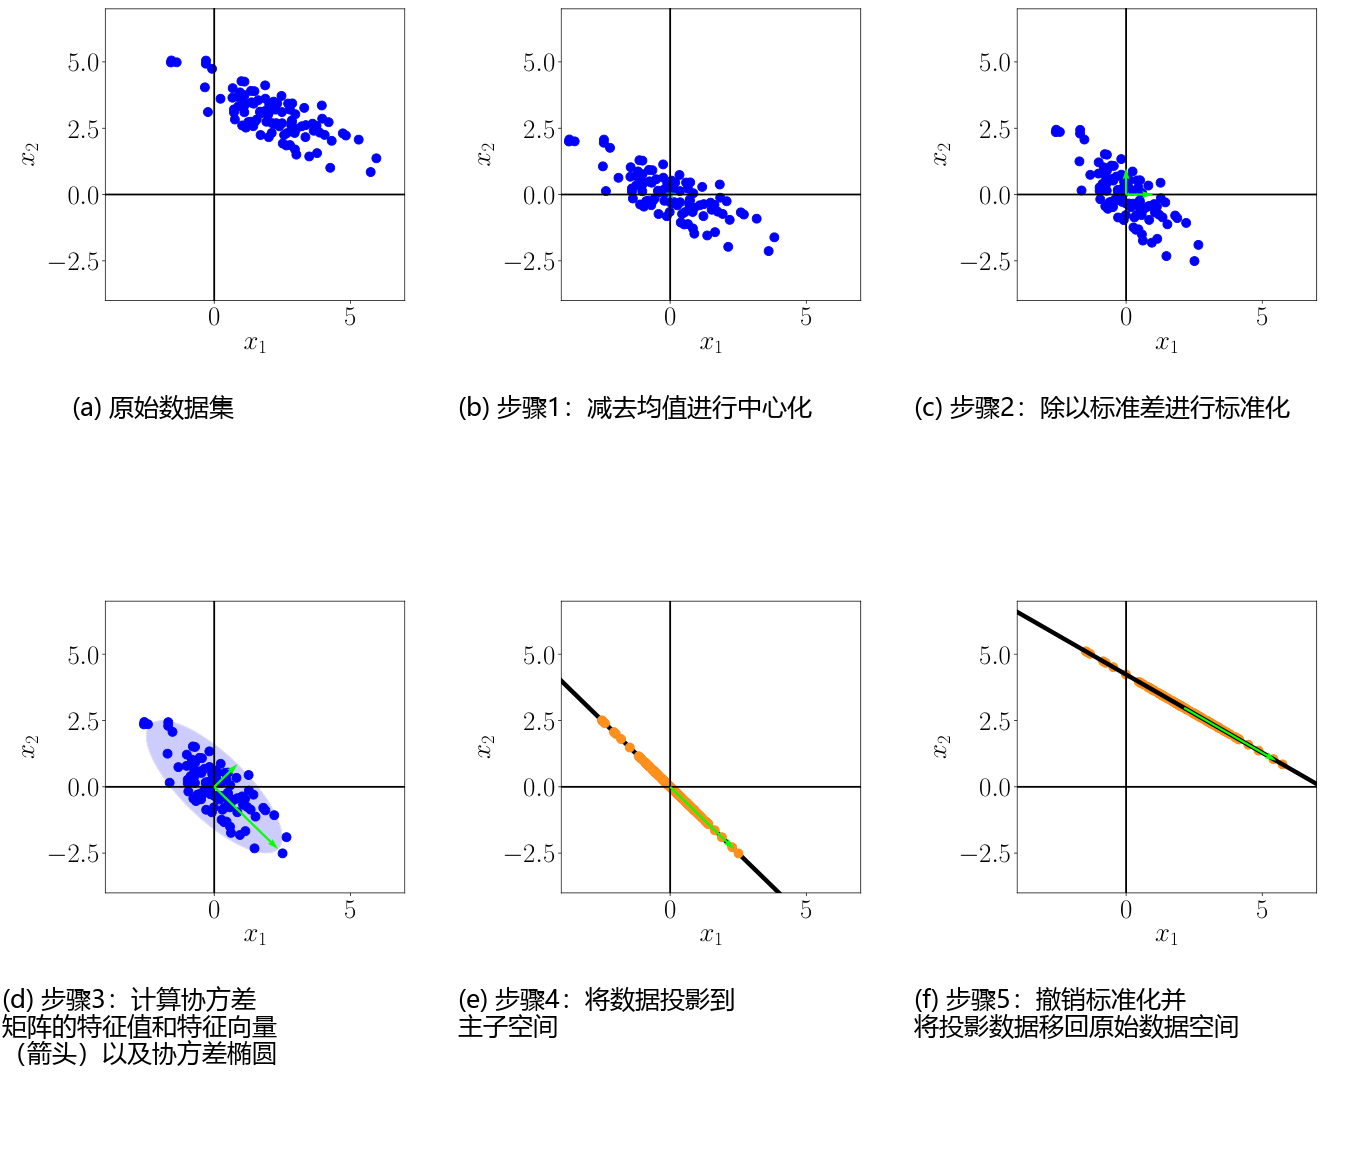
\includegraphics[width=0.92\textwidth,keepaspectratio]{docs/images/Figure10.11.png}
\caption*{图 10.11}
\end{figure}


\begin{enumerate}
\item \textbf{去均值中心化（Mean Subtraction）}：我们首先计算数据集的样本均值向量 $ \boldsymbol{\mu} $，并从每一个数据点中减去该均值。这确保了中心化后的数据集样本均值严格为 $ \boldsymbol{0} $（图 10.11(b)）。去均值操作虽然并非在所有理论定义中都不可或缺，但它能显著降低数值病态和精度下溢的风险。
\item \textbf{方差标准化（Standardization）}：对于每个维度 $ d = 1, \ldots, D $，将数据除以该维度上的样本标准差 $ \sigma_d $。经过此步骤，数据变得无量纲化，且沿各个坐标轴的方差均为 1，如图 10.11(c) 中的两个等长箭头所示。该步骤完成了数据的标准化预处理。
\item \textbf{协方差矩阵的特征分解（Eigendecomposition of the Covariance Matrix）}：计算标准化数据的样本协方差矩阵及其对应的特征值与特征向量。由于协方差矩阵是对称矩阵，谱定理（定理 4.15）保证我们可以找到一组标准正交特征基。在图 10.11(d) 中，特征向量按对应特征值的大小进行了尺度缩放。较长的特征向量张成了主子空间 $ U $。协方差矩阵的等高线由椭圆直观呈现。
\item \textbf{正交投影（Projection）}：现在我们可以将任意新数据点 $ \boldsymbol{x}_* \in \mathbb{R}^D $ 投影到主子空间上。为了保证量纲与训练阶段完全一致，我们需要首先使用训练数据的均值 $ \mu_d $ 和标准差 $ \sigma_d $ 对 $ \boldsymbol{x}_* $ 进行标准化：
\end{enumerate}

\begin{equation}
x_*^{(d)} \leftarrow \frac{x_*^{(d)} - \mu_d}{\sigma_d} , \quad d = 1, \ldots, D
\tag{10.58}
\end{equation}

其中 $ x_*^{(d)} $ 是 $ \boldsymbol{x}_* $ 的第 $ d $ 个分量。标准化后，我们在主子空间上的正交投影点为：

\begin{equation}
\tilde{\boldsymbol{x}}_* = \boldsymbol{B}\boldsymbol{B}^\top \boldsymbol{x}_*
\tag{10.59}
\end{equation}

其关于主子空间基向量的低维坐标向量为：

\begin{equation}
\boldsymbol{z}_* = \boldsymbol{B}^\top \boldsymbol{x}_* .
\tag{10.60}
\end{equation}

在此，矩阵 $ \boldsymbol{B} $ 的列向量包含协方差矩阵对应于最大特征值的特征向量。PCA 最终输出的是紧凑的低维坐标编码 (10.60)，而非高维重构点 $ \tilde{\boldsymbol{x}}_* $。

由于我们的模型建立在标准化数据集之上，式 (10.59) 给出的仅是标准化空间中的投影。若要在原始物理数据空间（即标准化之前）中获得重构点，我们需要撤销标准化操作 (10.58)：先乘以标准差，再加上均值：

\begin{equation}
\tilde{x}_*^{(d)} \leftarrow \tilde{x}_*^{(d)}\sigma_d + \mu_d , \quad d = 1, \ldots, D .
\tag{10.61}
\end{equation}

图 10.11(f) 展示了映射回原始数据空间后的最终投影重构结果。

\begin{notebox}
\textbf{例 10.4（MNIST 数字：图像重构）}
\end{notebox}

\begin{notebox}
接下来，我们将 PCA 应用于 MNIST 手写数字数据集。该数据集包含 60,000 个手写数字 0 到 9 的图像，每个图像大小为 $ 28 \times 28 $（共 784 个像素），因此可视为高维向量 $ \boldsymbol{x} \in \mathbb{R}^{784} $。
\end{notebox}

\begin{notebox}
出于演示目的，我们选取数字“8”的 5,389 张训练图像，按照前述步骤确定主子空间，并使用学习到的投影矩阵重构一组测试图像，如图 10.12 所示。
\end{notebox}


\begin{figure}[H]
\centering
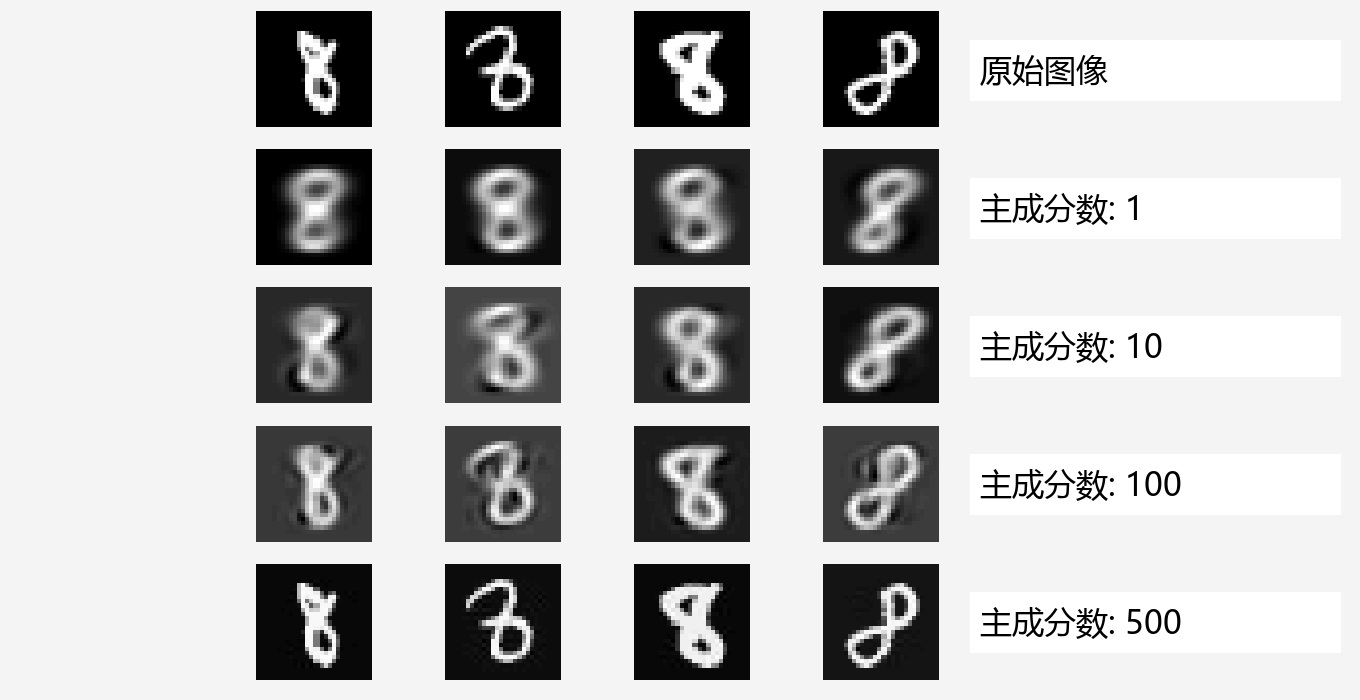
\includegraphics[width=0.92\textwidth,keepaspectratio]{docs/images/Figure10.12.png}
\caption*{图 10.12}
\end{figure}


图 10.12 的第一行展示了测试集中的 4 个原始数字图像。随后各行分别展示了使用 1、10、100 和 500 个主成分的重构结果。我们清晰地看到：即便仅使用单一的一维主子空间，我们也能获得原始数字轮廓的一个粗略但可辨识的重构（略显模糊和泛化）；随着主成分数量的增加，重构图像迅速变得锐利，笔画细节被完整保留；当增加至 500 个主成分时，重构效果几乎与原始图像无异。若选用全部 784 个主成分，则重构误差为零，实现 100\% 无损复原。

图 10.13 展示了平均平方重构误差随主成分个数 $ M $ 的变化曲线：

\begin{equation}
\frac{1}{N}\sum_{n=1}^N \|\boldsymbol{x}_n - \tilde{\boldsymbol{x}}_n\|^2 = \sum_{i=M+1}^D \lambda_i .
\tag{10.62}
\end{equation}


\begin{figure}[H]
\centering
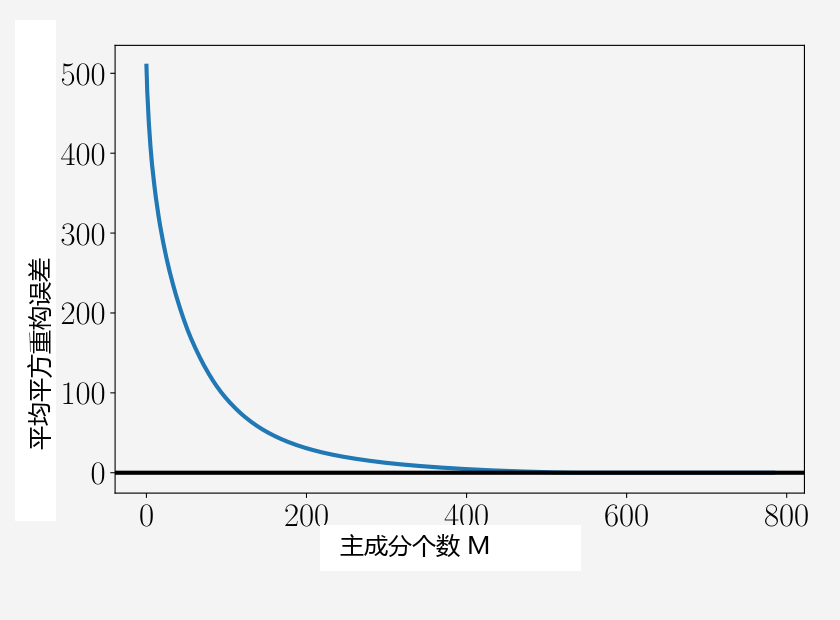
\includegraphics[width=0.92\textwidth,keepaspectratio]{docs/images/Figure10.13.png}
\caption*{图 10.13}
\end{figure}


我们可以发现，主成分的重要性呈现出指数级骤降，在达到一定数量后，继续增加主成分所带来的信息增益极其微小。这与我们在图 10.5 中的发现完全契合——绝大部分数据方差仅由少数前列的主成分所主导。在选用约 550 个主成分时，重构误差已基本归零（数字边缘周围的像素在整个数据集中始终为黑色，方差本就为 0）。

\section*{10.7 隐变量视角}
\addcontentsline{toc}{section}{10.7 隐变量视角}
\label{sec:10.7}

在前面的小节中，我们从最大方差和投影几何两个视角推导了 PCA，这两个视角完全没有引入任何概率模型的概念。一方面，这种确定性的几何推导非常吸引人，因为它绕开了概率论中复杂的积分与推断运算；但另一方面，构建一个显式的概率模型将为我们提供更强大的建模灵活性以及深刻的理论洞见。具体而言，概率模型能够：

\begin{enumerate}
\item 提供显式的似然函数，从而能够原则性地处理带噪声观测（我们在之前的几何推导中甚至未讨论噪声建模）；
\item 借助 8.6 节讨论的边缘似然执行严格的贝叶斯模型选择与维度比较；
\item 将 PCA 解释为一种 \emph{生成模型（generative model）} ，使我们能够自主采样并模拟合成全新的数据样本；
\item 建立与因子分析（Factor Analysis）等密切相关经典模型的直接数学桥梁；
\item 借助贝叶斯定理自然处理随机缺失某些维度特征的不完整数据；
\item 量化测试数据点的新颖度（用于异常检测与离群点识别）；
\item 提供原则性的模型拓展框架（例如高斯混合 PCA 模型）；
\item 将经典 PCA 作为零噪声极限下的一个特例完美涵盖；
\item 允许通过对模型参数进行边缘化积分开展全贝叶斯推断。
\end{enumerate}

通过引入一个连续型 \emph{隐变量（latent variable）} $ \boldsymbol{z} \in \mathbb{R}^M $，我们可以将 PCA 严谨表述为一个概率隐变量模型。Tipping and Bishop (1999) 提出了这一框架，称之为 \emph{概率主成分分析（probabilistic PCA, PPCA）} 。PPCA 完美解决了上述所有理论问题，我们在前文中通过最大化投影方差或最小化重构误差所得的传统 PCA 解，正是 PPCA 在无噪声极限下的极大似然估计特例。

\medskip\hrule\medskip

\section*{10.7.1 生成过程与概率模型}
\addcontentsline{toc}{subsection}{10.7.1 生成过程与概率模型}

在 PPCA 中，我们显式构建用于线性降维的概率模型。为此，我们假设一个连续隐变量 $ \boldsymbol{z} \in \mathbb{R}^M $，其先验分布为标准多元正态分布 $ p(\boldsymbol{z}) = \mathcal{N}(\boldsymbol{0}, \boldsymbol{I}) $，并且隐变量与观测数据 $ \boldsymbol{x} \in \mathbb{R}^D $ 之间满足如下仿射生成关系：

\begin{equation}
\boldsymbol{x} = \boldsymbol{B}\boldsymbol{z} + \boldsymbol{\mu} + \boldsymbol{\epsilon} \in \mathbb{R}^D
\tag{10.63}
\end{equation}

其中 $ \boldsymbol{\epsilon} \sim \mathcal{N}(\boldsymbol{0}, \sigma^2\boldsymbol{I}) $ 是各向同性高斯测量噪声，$ \boldsymbol{B} \in \mathbb{R}^{D \times M} $ 与 $ \boldsymbol{\mu} \in \mathbb{R}^D $ 描述了从低维隐空间到高维观测空间的线性/仿射映射。因此，PPCA 通过如下条件似然将隐变量与观测变量联系起来：

\begin{equation}
p(\boldsymbol{x} \mid \boldsymbol{z}, \boldsymbol{B}, \boldsymbol{\mu}, \sigma^2) = \mathcal{N}\left(\boldsymbol{x} \mid \boldsymbol{B}\boldsymbol{z} + \boldsymbol{\mu}, \sigma^2\boldsymbol{I}\right) .
\tag{10.64}
\end{equation}

PPCA 诱导了如下清晰的先祖数据生成机制（ancestral sampling）：

\begin{equation}
\boldsymbol{z}_n \sim \mathcal{N}(\boldsymbol{z} \mid \boldsymbol{0}, \boldsymbol{I})
\tag{10.65}
\end{equation}

\begin{equation}
\boldsymbol{x}_n \mid \boldsymbol{z}_n \sim \mathcal{N}\left(\boldsymbol{x} \mid \boldsymbol{B}\boldsymbol{z}_n + \boldsymbol{\mu}, \sigma^2\boldsymbol{I}\right) .
\tag{10.66}
\end{equation}

为了生成符合模型参数的数据样本，我们遵循先祖采样：首先从先验 $ p(\boldsymbol{z}) $ 中采样一个隐变量 $ \boldsymbol{z}_n $，然后以采样出的 $ \boldsymbol{z}_n $ 为条件，利用式 (10.64) 采样观测数据点 $ \boldsymbol{x}_n $。

该生成过程构成了完整的联合概率分布：

\begin{equation}
p(\boldsymbol{x}, \boldsymbol{z} \mid \boldsymbol{B}, \boldsymbol{\mu}, \sigma^2) = p(\boldsymbol{x} \mid \boldsymbol{z}, \boldsymbol{B}, \boldsymbol{\mu}, \sigma^2)p(\boldsymbol{z})
\tag{10.67}
\end{equation}

对应于图 10.14 所示的概率有向图模型。


\begin{figure}[H]
\centering
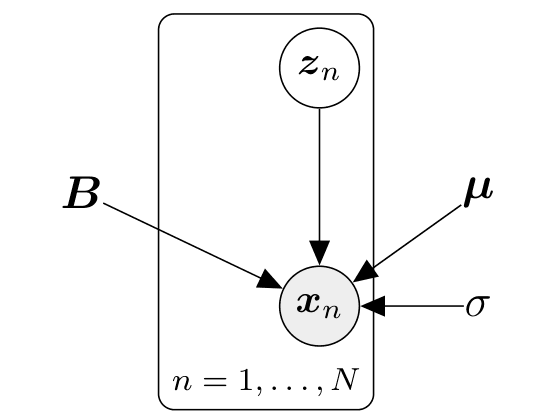
\includegraphics[width=0.92\textwidth,keepaspectratio]{docs/images/Figure10.14.png}
\caption*{图 10.14}
\end{figure}


\emph{备注} （箭头的因果方向） 。请特别注意连接隐变量 $ \boldsymbol{z} $ 与观测数据 $ \boldsymbol{x} $ 的箭头方向：箭头由 $ \boldsymbol{z} $ 指向 $ \boldsymbol{x} $，这意味着 PPCA 模型假设低维隐变量 $ \boldsymbol{z} $ 是产生高维复杂观测 $ \boldsymbol{x} $ 的“潜在诱因”（latent cause）。而在降维任务中，我们显然希望在给定观测 $ \boldsymbol{x} $ 的前提下反推 $ \boldsymbol{z} $。为了达成这一目的，我们将运用贝叶斯推断隐式地“翻转”箭头，实现从观测到潜在编码的逆向推断。

\begin{notebox}
\textbf{例 10.5（利用隐变量生成新数据）}
\end{notebox}

\begin{notebox}
图 10.15 展示了利用二维主子空间（蓝点）获得的 MNIST 数字“8”的隐空间二维坐标。我们可以在该隐空间中任意指定一个向量 $ \boldsymbol{z}_* $，并通过 $ \tilde{\boldsymbol{x}}_* = \boldsymbol{B}\boldsymbol{z}_* $ 生成一张形似数字“8”的全新图像。
\end{notebox}

\begin{notebox}
我们展示了 8 张根据隐空间采样生成的数字图像及其对应的潜在坐标。随着我们在隐空间中移动采样位置，生成的图像平滑展现出形态、旋转角度与笔画粗细的连续演变。如果我们远离训练数据密集的区域进行外推采样，图像中便会出现明显的瑕疵和伪影。需要强调的是，这些生成图像的内在自由度严格只有 2 维。
\end{notebox}


\begin{figure}[H]
\centering
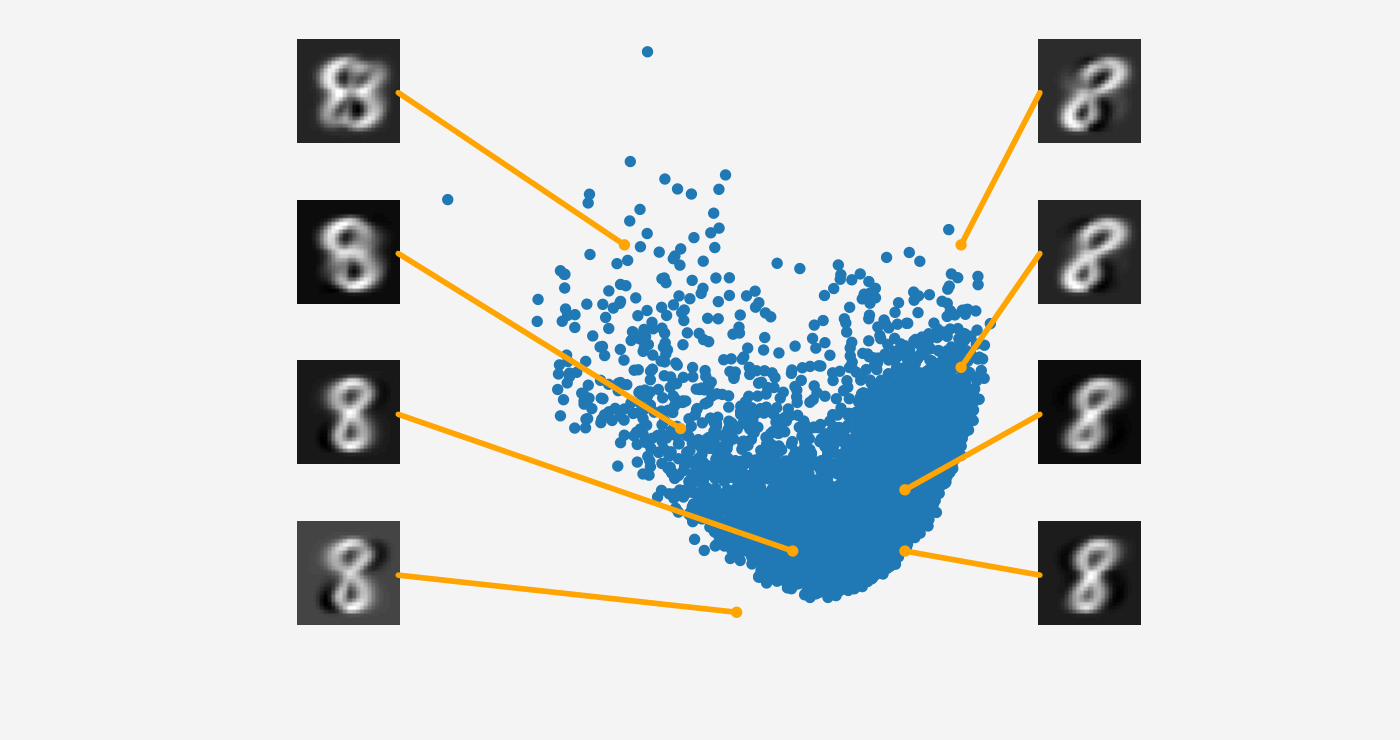
\includegraphics[width=0.92\textwidth,keepaspectratio]{docs/images/Figure10.15.png}
\caption*{图 10.15}
\end{figure}


\medskip\hrule\medskip

\section*{10.7.2 似然与联合分布}
\addcontentsline{toc}{subsection}{10.7.2 似然与联合分布}

利用第 6 章的结果，我们通过边缘化积分离出隐变量 $ \boldsymbol{z} $ 来获得该概率模型的边际似然函数（见 8.4.3 节）：

\begin{equation}
p(\boldsymbol{x} \mid \boldsymbol{B}, \boldsymbol{\mu}, \sigma^2) = \int p(\boldsymbol{x} \mid \boldsymbol{z}, \boldsymbol{\mu}, \sigma^2)p(\boldsymbol{z}) \mathrm{d}\boldsymbol{z}
\tag{10.68a}
\end{equation}

\begin{equation}
= \int \mathcal{N}\left(\boldsymbol{x} \mid \boldsymbol{B}\boldsymbol{z} + \boldsymbol{\mu}, \sigma^2\boldsymbol{I}\right) \mathcal{N}(\boldsymbol{z} \mid \boldsymbol{0}, \boldsymbol{I}) \mathrm{d}\boldsymbol{z} .
\tag{10.68b}
\end{equation}

由 6.5 节可知，该积分是一个高斯分布，其期望均值为：

\begin{equation}
\mathbb{E}_{\boldsymbol{x}}[\boldsymbol{x}] = \mathbb{E}_{\boldsymbol{z}}[\boldsymbol{B}\boldsymbol{z} + \boldsymbol{\mu}] + \mathbb{E}_{\boldsymbol{\epsilon}}[\boldsymbol{\epsilon}] = \boldsymbol{\mu}
\tag{10.69}
\end{equation}

其协方差矩阵为：

\begin{equation}
\begin{adjustbox}{max width=\linewidth}
\mathbb{V}[\boldsymbol{x}] = \mathbb{V}_{\boldsymbol{z}}[\boldsymbol{B}\boldsymbol{z} + \boldsymbol{\mu}] + \mathbb{V}_{\boldsymbol{\epsilon}}[\boldsymbol{\epsilon}] = \boldsymbol{B}\mathbb{V}_{\boldsymbol{z}}[\boldsymbol{z}]\boldsymbol{B}^\top + \sigma^2\boldsymbol{I}
\end{adjustbox}
\tag{10.70a}
\end{equation}

\begin{equation}
= \boldsymbol{B}\boldsymbol{B}^\top + \sigma^2\boldsymbol{I} .
\tag{10.70b}
\end{equation}

式 (10.68b) 中的边际似然函数可用于模型参数的极大似然或 MAP 估计。

\emph{备注} 。我们不能直接使用式 (10.64) 的条件似然来进行参数估计，因为它仍然显式包含未知的隐变量。极大似然估计所要求的似然函数必须仅是观测数据 $ \boldsymbol{x} $ 与模型参数的函数，必须通过积分消除对隐变量的依赖。

高斯随机变量 $ \boldsymbol{z} $ 及其仿射变换 $ \boldsymbol{x} = \boldsymbol{B}\boldsymbol{z} + \boldsymbol{\mu} + \boldsymbol{\epsilon} $ 服从联合高斯分布。其互协方差为：

\begin{equation}
\text{Cov}[\boldsymbol{x}, \boldsymbol{z}] = \text{Cov}_{\boldsymbol{z}}[\boldsymbol{B}\boldsymbol{z} + \boldsymbol{\mu}, \boldsymbol{z}] = \boldsymbol{B}\text{Cov}[\boldsymbol{z}, \boldsymbol{z}] = \boldsymbol{B} .
\tag{10.71}
\end{equation}

因此，PPCA 的联合高斯概率分布显式表示为：

\begin{equation}
\begin{adjustbox}{max width=\linewidth}
p(\boldsymbol{x}, \boldsymbol{z} \mid \boldsymbol{B}, \boldsymbol{\mu}, \sigma^2) = \mathcal{N}\left( \begin{bmatrix} \boldsymbol{x} \\ \boldsymbol{z} \end{bmatrix} \;\middle|\; \begin{bmatrix} \boldsymbol{\mu} \\ \boldsymbol{0} \end{bmatrix} , \begin{bmatrix} \boldsymbol{B}\boldsymbol{B}^\top + \sigma^2\boldsymbol{I} & \boldsymbol{B} \\ \boldsymbol{B}^\top & \boldsymbol{I} \end{bmatrix} \right) .
\end{adjustbox}
\tag{10.72}
\end{equation}

\medskip\hrule\medskip

\section*{10.7.3 后验分布}
\addcontentsline{toc}{subsection}{10.7.3 后验分布}

借助式 (10.72) 中的联合高斯分布，我们利用 6.5.1 节的高斯条件分布公式，可以立即求得在给定观测 $ \boldsymbol{x} $ 时隐变量的后验概率分布：

\begin{equation}
p(\boldsymbol{z} \mid \boldsymbol{x}) = \mathcal{N}\left(\boldsymbol{z} \mid \boldsymbol{m}, \boldsymbol{C}\right)
\tag{10.73}
\end{equation}

其中后验均值与后验协方差矩阵分别为：

\begin{equation}
\boldsymbol{m} = \boldsymbol{B}^\top\left(\boldsymbol{B}\boldsymbol{B}^\top + \sigma^2\boldsymbol{I}\right)^{-1}(\boldsymbol{x} - \boldsymbol{\mu})
\tag{10.74}
\end{equation}

\begin{equation}
\boldsymbol{C} = \boldsymbol{I} - \boldsymbol{B}^\top\left(\boldsymbol{B}\boldsymbol{B}^\top + \sigma^2\boldsymbol{I}\right)^{-1}\boldsymbol{B} .
\tag{10.75}
\end{equation}

值得注意的是，后验协方差矩阵 $ \boldsymbol{C} $ 完全独立于具体的观测数据 $ \boldsymbol{x} $。对于数据空间中的任意新观测 $ \boldsymbol{x}_* $，我们利用式 (10.73) 即可求得对应低维隐编码 $ \boldsymbol{z}_* $ 的后验分布。后验协方差矩阵 $ \boldsymbol{C} $ 允许我们定量评估低维嵌入的置信程度：行列式 $ \det(\boldsymbol{C}) $ 越小，说明隐变量嵌入的不确定性越小、确定度越高；若某个样本导出了极高方差的后验分布，则该点很可能是数据空间中的异常离群点。

更进一步，我们可以利用 PPCA 的生成机制探索隐变量后验分布的物理含义，即假想并生成在该后验下所有合理的数据形态：

\begin{enumerate}
\item 从隐变量后验分布 (10.73) 中采样潜在编码 $ \boldsymbol{z}_* \sim p(\boldsymbol{z} \mid \boldsymbol{x}_*) $；
\item 利用式 (10.64) 采样重构的高维向量 $ \tilde{\boldsymbol{x}}_* \sim p(\boldsymbol{x} \mid \boldsymbol{z}_*, \boldsymbol{B}, \boldsymbol{\mu}, \sigma^2) $。
\end{enumerate}

反复重复此采样过程，便可在数据空间中完整生成符合后验置信假设的所有可能高维数据形态。

\section*{10.8 延伸阅读}
\addcontentsline{toc}{section}{10.8 延伸阅读}
\label{sec:10.8}

我们在本章中从两个主要几何视角推导了 PCA：(a) 最大化投影空间中的方差；(b) 最小化平均重构误差。然而，PCA 还可以从许多其他重要学科的视角进行阐释与拓展。

\section*{作为线性自动编码器的 PCA}
\addcontentsline{toc}{subsection}{作为线性自动编码器的 PCA}

如图 10.16 所示，我们可以将 PCA 视为一个 \emph{线性自动编码器（linear auto-encoder）} 。自动编码器首先通过编码器将高维数据 $ \boldsymbol{x}_n \in \mathbb{R}^D $ 编码为低维编码 $ \boldsymbol{z}_n \in \mathbb{R}^M $，然后通过解码器将其解算回与 $ \boldsymbol{x}_n $ 相似的重构数据 $ \tilde{\boldsymbol{x}}_n $。


\begin{figure}[H]
\centering
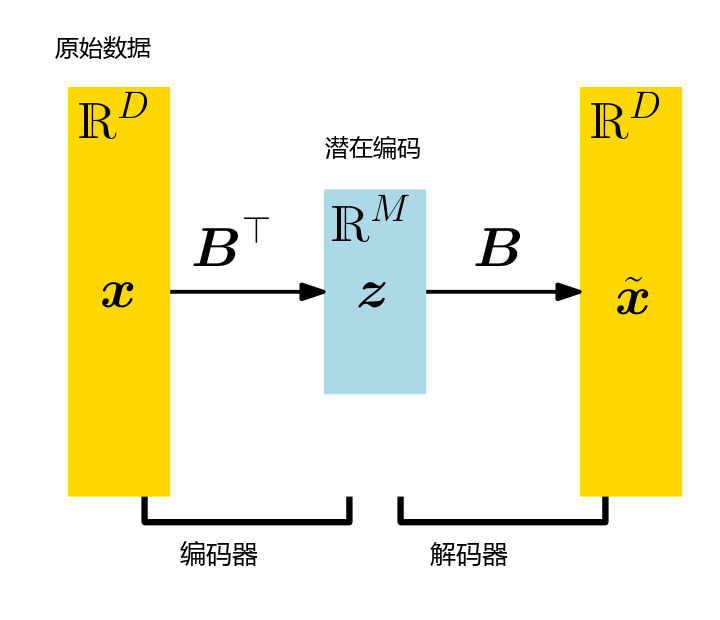
\includegraphics[width=0.92\textwidth,keepaspectratio]{docs/images/Figure10.16.png}
\caption*{图 10.16}
\end{figure}


当我们考虑线性编码映射 $ \boldsymbol{z}_n = \boldsymbol{B}^\top \boldsymbol{x}_n $ 与线性解码映射 $ \tilde{\boldsymbol{x}}_n = \boldsymbol{B}\boldsymbol{z}_n $，并优化最小化平均平方重构误差：

\begin{equation}
\frac{1}{N}\sum_{n=1}^N \|\boldsymbol{x}_n - \tilde{\boldsymbol{x}}_n\|^2 = \frac{1}{N}\sum_{n=1}^N \|\boldsymbol{x}_n - \boldsymbol{B}\boldsymbol{B}^\top \boldsymbol{x}_n\|^2
\tag{10.76}
\end{equation}

该目标函数与我们在 10.3 节讨论的式 (10.29) 完全相同。因此，最小化线性自动编码器的平方重构损失直接导出了 PCA 解。若将线性映射替换为非线性映射（例如多层前馈深度神经网络），便自然得到了 \emph{深度自动编码器（deep auto-encoder）} 。在深度学习语境中，编码器通常被称为识别网络（recognition network）或推断网络（inference network），而解码器则被称为生成器（generator）。

\section*{信息论视角}
\addcontentsline{toc}{subsection}{信息论视角}

另一种解释来源于信息论。我们可以将编码视为原始数据的有损压缩版本。直观上，为了在压缩后保留最多的信息，我们希望最大化原始高维数据与低维编码之间的 \emph{互信息（mutual information）} 。信息论证明，在特定高斯假设下，最大化互信息所求得的最优线性映射与 PCA 解完全一致（MacKay, 2003）。

\section*{概率 PCA 的参数估计与零噪声极限}
\addcontentsline{toc}{subsection}{概率 PCA 的参数估计与零噪声极限}

在 10.7 节对 PPCA 的讨论中，我们假设参数 $ \boldsymbol{B}\textcn{、}\boldsymbol{\mu} $ 及噪声参数 $ \sigma^2 $ 是已知的。Tipping and Bishop (1999) 给出了在 PPCA 框架下这些参数的极大似然解析闭式解：

\begin{equation}
\boldsymbol{\mu}_{\text{ML}} = \frac{1}{N}\sum_{n=1}^N \boldsymbol{x}_n
\tag{10.77}
\end{equation}

\begin{equation}
\boldsymbol{B}_{\text{ML}} = \boldsymbol{T}\left(\boldsymbol{\Lambda} - \sigma^2\boldsymbol{I}\right)^{\frac{1}{2}}\boldsymbol{R}
\tag{10.78}
\end{equation}

\begin{equation}
\sigma_{\text{ML}}^2 = \frac{1}{D - M}\sum_{j=M+1}^D \lambda_j
\tag{10.79}
\end{equation}

其中 $ \boldsymbol{T} \in \mathbb{R}^{D \times M} $ 包含数据协方差矩阵的 $ M $ 个主特征向量，$ \boldsymbol{\Lambda} = \text{diag}(\lambda_1, \ldots, \lambda_M) \in \mathbb{R}^{M \times M} $ 是对角线上排列着主特征值的对角矩阵，$ \boldsymbol{R} \in \mathbb{R}^{M \times M} $ 是任意的正交旋转矩阵。极大似然解 $ \boldsymbol{B}_{\text{ML}} $ 在旋转意义下是唯一的（右乘任意旋转矩阵 $ \boldsymbol{R} $ 依然成立），这直接对应了奇异值分解的结构。式 (10.79) 揭示出：观测噪声方差的极大似然估计，恰好等于主子空间正交补空间中所有被丢弃特征值的算术平均值！即 PCA 无法捕获的剩余方差在概率模型中被统统视为各向同性白噪声。

在无噪声极限（$ \sigma \to 0 $）下，PPCA 与传统 PCA 完全重合。由于数据协方差矩阵 $ \boldsymbol{S} $ 是对称矩阵，因此可以将其对角化，即存在由 $ \boldsymbol{S} $ 的特征向量组成的矩阵 $ \boldsymbol{T} $，使得：

\begin{equation}
\boldsymbol{S} = \boldsymbol{T}\boldsymbol{\Lambda}\boldsymbol{T}^{-1} .
\tag{10.80}
\end{equation}

PPCA 模型中的数据协方差为 $ \boldsymbol{B}\boldsymbol{B}^\top + \sigma^2\boldsymbol{I} $。当 $ \sigma \to 0 $ 时，它必须与 PCA 的数据协方差及其式 (10.80) 中的分解相等，因此：

\begin{equation}
\begin{adjustbox}{max width=\linewidth}
\operatorname{Cov}[\mathcal{X}] = \boldsymbol{T}\boldsymbol{\Lambda}\boldsymbol{T}^{-1} = \boldsymbol{B}\boldsymbol{B}^\top \quad \Longleftrightarrow \quad \boldsymbol{B} = \boldsymbol{T}\boldsymbol{\Lambda}^{\frac{1}{2}}\boldsymbol{R} .
\end{adjustbox}
\tag{10.81}
\end{equation}

这也就得到了 $ \sigma = 0 $ 时式 (10.78) 的极大似然估计。对于在线流式数据，可采用 EM 期望最大化算法进行迭代参数估计（Roweis, 1998）。

关于内在维度 $ M $ 的确定，Gavish and Donoho (2014) 提出了基于噪声估计的截断启发式规则：若已知数据噪声标准差 $ \sigma $，应丢弃所有小于 $ 4\sigma\sqrt{D}/\sqrt{3} $ 的奇异值。此外，嵌套交叉验证（8.6.1 节）与贝叶斯模型证据准则（8.6.2 节）也是估计数据内在维度的有力工具（Minka, 2001b）。

\section*{贝叶斯 PCA 与因子分析、独立成分分析}
\addcontentsline{toc}{subsection}{贝叶斯 PCA 与因子分析、独立成分分析}

进一步地，我们可以在模型参数上引入先验分布并将其边缘化积分离出，从而得到 \emph{贝叶斯 PCA（Bayesian PCA）} （Bishop, 1999）。该方法避免了点估计引起的过拟合，并能自动通过贝叶斯奥卡姆剃刀剪枝冗余的主成分，实现内在维度 $ M $ 的自动学习。

如果我们在 PPCA 的观测模型 $ \boldsymbol{x}_n \mid \boldsymbol{z}_n \sim \mathcal{N}(\boldsymbol{B}\boldsymbol{z}_n + \boldsymbol{\mu}, \boldsymbol{\Sigma}) $ 中，允许各个观测维度拥有不同的噪声方差（即对角噪声协方差矩阵 $ \boldsymbol{\Sigma} = \text{diag}(\sigma_1^2, \ldots, \sigma_D^2) $），我们便得到了经典的 \emph{因子分析（factor analysis, FA）} （Spearman, 1904; Bartholomew et al., 2011）。与 PPCA 相比，因子分析具有尺度不变性，但在正交旋转下不再具有旋转不变性。

若将隐变量的先验分布由高斯分布改为非高斯分布，则导出了 \emph{独立成分分析（independent component analysis, ICA）} （Hyvarinen et al., 2001）。ICA 广泛应用于盲源分离（blind-source separation，如经典的“鸡尾酒会问题”），能够打破 PCA 的正交旋转不确定性，分离出独立的真实信号源。关于线性降维模型的更全面综述，可参阅 Cunningham and Ghahramani (2015)。

\section*{核 PCA 与高斯过程隐变量模型（GP-LVM）}
\addcontentsline{toc}{subsection}{核 PCA 与高斯过程隐变量模型（GP-LVM）}

借助核技巧（kernel trick），我们可以将特征内积推广至无限维希尔伯特空间，从而得到 \emph{核主成分分析（Kernel PCA）} （Schölkopf et al., 1998; Schölkopf and Smola, 2002），能够挖掘出高度复杂的非线性流形结构（Burges, 2010）。

另一条强大的非线性降维路线是 Lawrence (2005) 提出的 \emph{高斯过程隐变量模型（Gaussian process latent variable model, GP-LVM）} 。GP-LVM 从 PPCA 的隐变量视角出发，将隐变量 $ \boldsymbol{z} $ 到观测 $ \boldsymbol{x} $ 之间的线性映射替换为非参数高斯过程（GP）。随后，Titsias and Lawrence (2010) 提出了贝叶斯 GP-LVM，在隐变量上保持概率分布并使用变分推断将其积分离出，代表了现代非参数贝叶斯降维技术的前沿。

\chapter{11 使用高斯混合模型进行密度估计}

在前面的章节中，我们已经探讨了机器学习中两个基础的核心支柱问题：回归（第 9 章）与降维（第 10 章）。在本章中，我们将考察机器学习的第三大支柱： \emph{密度估计（density estimation）} 。在此过程中，我们将引入极其重要的核心概念，例如 \emph{期望最大化（expectation maximization, EM）} 算法以及基于混合模型的隐变量视角。

当我们对数据应用机器学习时，通常旨在以某种数学形式来表示数据。最直接的方法是将数据点本身作为数据的离散表示；图 11.1 给出了一个具体示例。然而，如果数据集极其庞大，或者我们感兴趣的是抽象提炼出数据的生成统计特征，这种离散罗列的方法便无能为力。在密度估计中，我们使用来自参数化概率分布族（如高斯分布、Beta 分布等）的概率密度函数来紧凑地表示数据。例如，我们可能寻求数据集的均值与方差，以便使用高斯分布来紧凑表示数据。均值与方差可以通过我们在 8.3 节讨论的极大似然估计或最大后验估计来求解。随后，我们可以使用该高斯分布的均值与方差来代表生成数据的底层分布，即认为该数据集是从该连续分布中随机抽样所得到的典型实现。


\begin{figure}[H]
\centering
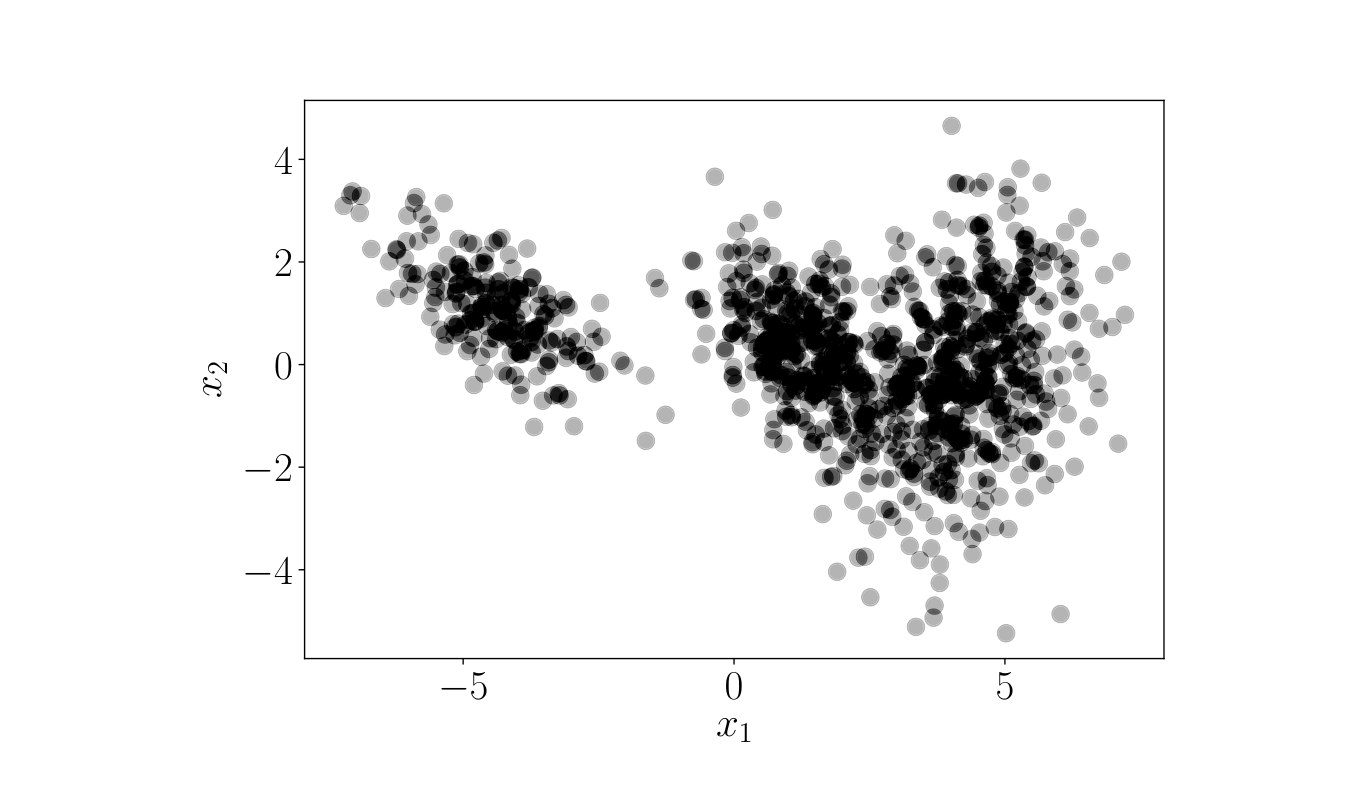
\includegraphics[width=0.92\textwidth,keepaspectratio]{docs/images/Figure11.1.png}
\caption*{图 11.1}
\end{figure}


然而在实践中，单一高斯分布（以及我们迄今为止见过的所有其他简单单峰分布）的建模表达能力非常有限。例如，若用单一高斯分布来近似生成图 11.1 数据的底层密度，拟合效果将会极其糟糕。为了解决这一局限性，在下文中我们将考察一类表达能力强得多的概率分布族： \emph{混合模型（mixture models）} 。

混合模型通过对 $ K $ 个简单的基分布（base distributions）进行凸组合（convex combination）来描述复杂概率分布 $ p(\boldsymbol{x}) $：

\begin{equation}
p(\boldsymbol{x}) = \sum_{k=1}^K \pi_k p_k(\boldsymbol{x})
\tag{11.1}
\end{equation}

\begin{equation}
0 \leqslant \pi_k \leqslant 1 , \quad \sum_{k=1}^K \pi_k = 1
\tag{11.2}
\end{equation}

其中分量 $ p_k $ 属于某种基础分布族（例如高斯分布、伯努利分布或 Gamma 分布），$ \pi_k $ 被称为 \emph{混合权重（mixture weights）} 。混合模型比对应的单个基分布表达能力丰富得多，因为它们能够表示 \emph{多峰数据（multimodal data）} ，即能够描述包含多个“簇”（clusters）的复杂数据集，如图 11.1 所示。

在本章中，我们将重点关注基分布为高斯分布的 \emph{高斯混合模型（Gaussian mixture models, GMM）} 。对于给定的数据集，我们的目标是最大化模型参数的似然函数来训练 GMM。为此，我们将系统运用第 5 章的微积分、第 6 章的概率论以及 7.2 节的带约束优化工具。然而，与我们之前讨论的其他模型（线性回归或 PCA）截然不同的是，\textbf{高斯混合模型的极大似然估计不存在解析闭式解}！相反，求导将导出一组相互耦合的联立非线性方程组，我们只能通过迭代算法（即 EM 算法）对其进行数值求解。

在本章的后续部分：

\begin{itemize}
\item 11.1 节形式化高斯混合模型；
\item 11.2 节详细推导通过极大似然原理估计 GMM 均值、协方差和混合权重的梯度方程与联立自洽方程；
\item 11.3 节正式给出并剖析 EM 算法的完整执行流程及数值表现；
\item 11.4 节从隐变量模型和 Jensen 不等式的更广义视角深入阐释 EM 算法的理论下界保障；
\item 11.5 节提供延伸阅读。
\end{itemize}

\section*{11.1 高斯混合模型}
\addcontentsline{toc}{section}{11.1 高斯混合模型}
\label{sec:11.1}

\emph{高斯混合模型（Gaussian mixture model, GMM）} 是一种将有限数量（$ K $ 个）高斯分布 $ \mathcal{N}(\boldsymbol{x} \mid \boldsymbol{\mu}_k, \boldsymbol{\Sigma}_k) $ 进行凸组合的概率密度模型：

\begin{equation}
p(\boldsymbol{x} \mid \boldsymbol{\theta}) = \sum_{k=1}^K \pi_k \mathcal{N}\left(\boldsymbol{x} \mid \boldsymbol{\mu}_k, \boldsymbol{\Sigma}_k\right)
\tag{11.3}
\end{equation}

\begin{equation}
0 \leqslant \pi_k \leqslant 1 , \quad \sum_{k=1}^K \pi_k = 1
\tag{11.4}
\end{equation}

其中我们将 $ \boldsymbol{\theta} := \{\boldsymbol{\mu}_k, \boldsymbol{\Sigma}_k, \pi_k : k = 1, \ldots, K\} $ 定义为模型所有待估计参数的集合。与简单的单高斯分布（当 $ K = 1 $ 时从式 (11.3) 退化恢复得到）相比，高斯分布的这种凸组合赋予了模型表征高度复杂的多峰连续概率密度的强大灵活性。


\begin{figure}[H]
\centering
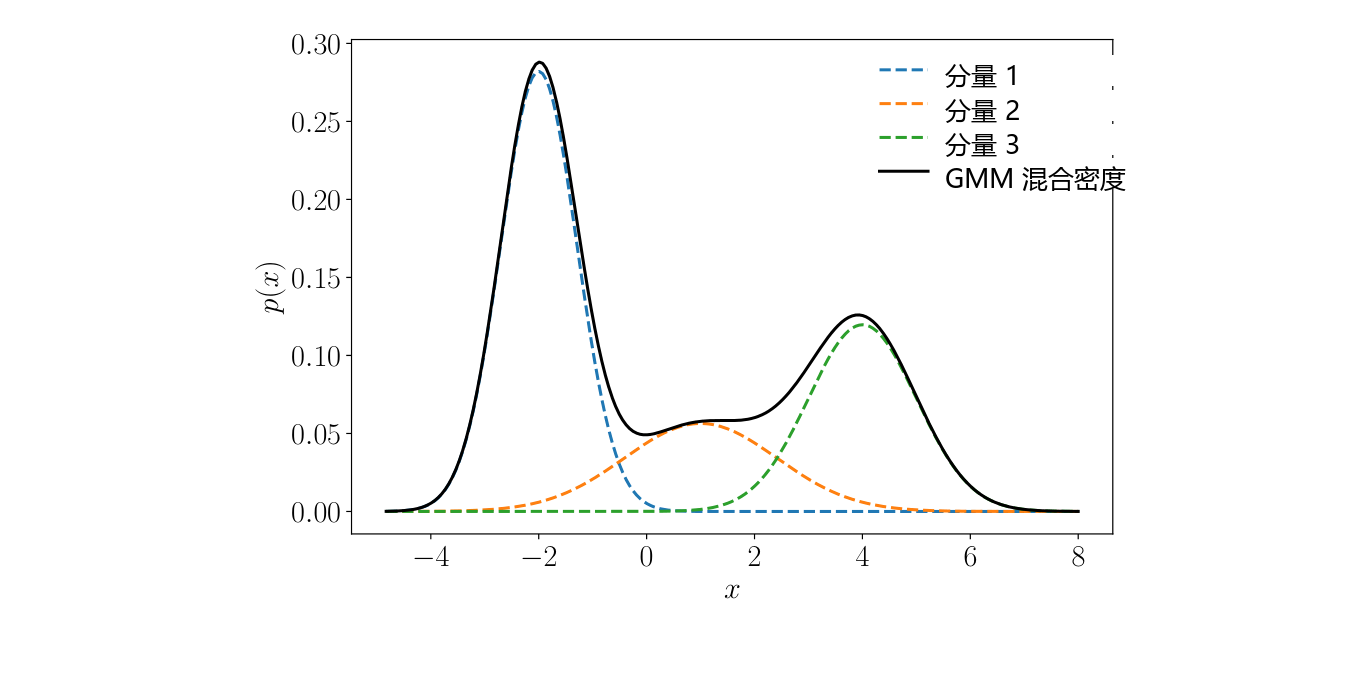
\includegraphics[width=0.92\textwidth,keepaspectratio]{docs/images/Figure11.2.png}
\caption*{图 11.2}
\end{figure}


图 11.2 直观图解了式 (11.3) 的 GMM 结构，展示了加权的高斯分量与总体的混合密度分布。在该一维示例中，混合密度显式表达为：

\begin{equation}
p(x \mid \boldsymbol{\theta}) = 0.5\mathcal{N}(x \mid -2, 1) + 0.2\mathcal{N}(x \mid 1, 2) + 0.3\mathcal{N}(x \mid 4, 1) .
\tag{11.5}
\end{equation}

在接下来的内容中，我们将探讨如何为给定的无监督观测数据集拟合高斯混合模型的参数。

\section*{11.2 通过极大似然进行参数学习}
\addcontentsline{toc}{section}{11.2 通过极大似然进行参数学习}
\label{sec:11.2}

我们考虑一个由 7 个数据点组成的一维数据集 $ \mathcal{X} = \{-3, -2.5, -1, 0, 2, 4, 5\} $，并希望寻找一个包含 $ K = 3 $ 个分量的高斯混合模型来拟合该数据的概率密度。我们将各个混合分量初始化为：

\begin{equation}
p_1(x) = \mathcal{N}(x \mid -4, 1)
\tag{11.6}
\end{equation}

\begin{equation}
p_2(x) = \mathcal{N}(x \mid 0, 0.2)
\tag{11.7}
\end{equation}

\begin{equation}
p_3(x) = \mathcal{N}(x \mid 8, 3)
\tag{11.8}
\end{equation}

并赋予它们相等的初始混合权重 $ \pi_1 = \pi_2 = \pi_3 = \frac{1}{3} $。对应的模型分布以及数据点在图 11.3 中展示。


\begin{figure}[H]
\centering
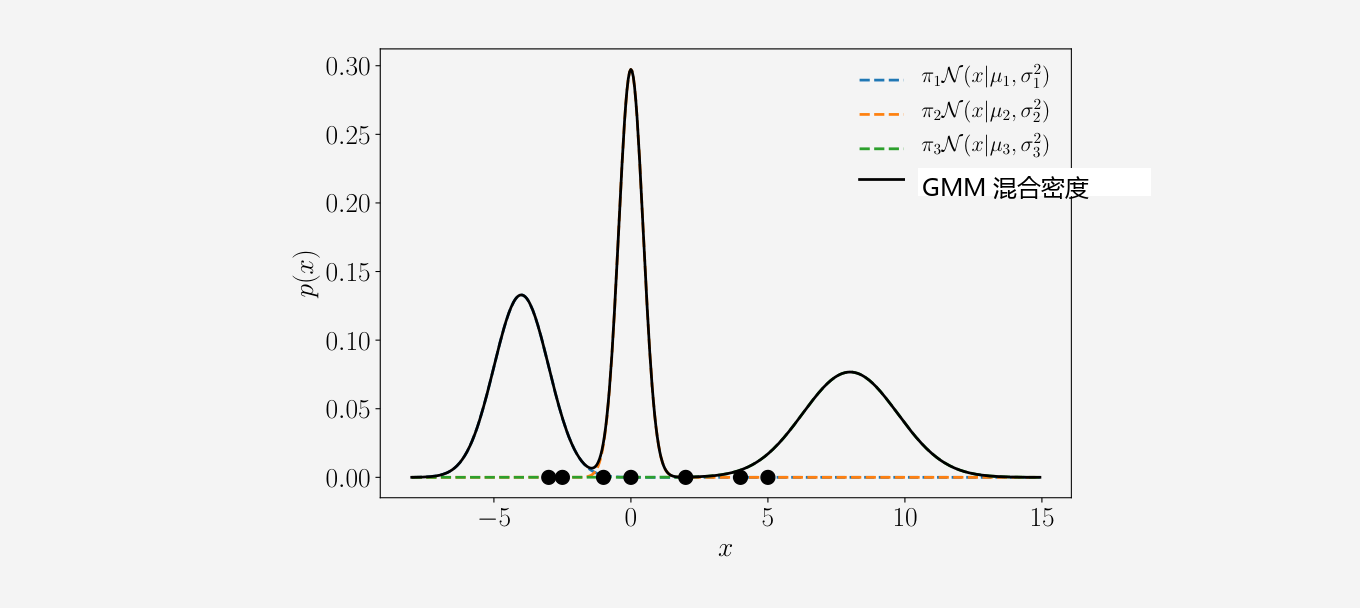
\includegraphics[width=0.92\textwidth,keepaspectratio]{docs/images/Figure11.3.png}
\caption*{图 11.3}
\end{figure}


在下文中，我们将详细阐述如何求解模型参数 $ \boldsymbol{\theta} $ 的极大似然估计 $ \boldsymbol{\theta}_{\text{ML}} $。我们首先写出似然函数，即在给定模型参数的条件下训练数据的联合概率密度。利用独立同分布（i.i.d.）假设，似然函数因式分解为：

\begin{equation}
\begin{adjustbox}{max width=\linewidth}
p(\mathcal{X} \mid \boldsymbol{\theta}) = \prod_{n=1}^N p(\boldsymbol{x}_n \mid \boldsymbol{\theta}) , \quad p(\boldsymbol{x}_n \mid \boldsymbol{\theta}) = \sum_{k=1}^K \pi_k \mathcal{N}\left(\boldsymbol{x}_n \mid \boldsymbol{\mu}_k, \boldsymbol{\Sigma}_k\right)
\end{adjustbox}
\tag{11.9}
\end{equation}

其中每一个样本点的似然项 $ p(\boldsymbol{x}_n \mid \boldsymbol{\theta}) $ 都是一个高斯混合密度。据此，对数似然函数表示为：

\begin{equation}
\begin{adjustbox}{max width=\linewidth}
\log p(\mathcal{X} \mid \boldsymbol{\theta}) = \sum_{n=1}^N \log p(\boldsymbol{x}_n \mid \boldsymbol{\theta}) = \underbrace{\sum_{n=1}^N \log \left( \sum_{k=1}^K \pi_k \mathcal{N}\left(\boldsymbol{x}_n \mid \boldsymbol{\mu}_k, \boldsymbol{\Sigma}_k\right) \right)}_{=: \mathcal{L}} .
\end{adjustbox}
\tag{11.10}
\end{equation}

我们的目标是寻找参数 $ \boldsymbol{\theta}_{\text{ML}}^* $ 以最大化式 (11.10) 中定义的对数似然 $ \mathcal{L} $。我们的“常规”解题套路是对模型参数 $ \boldsymbol{\theta} $ 计算对数似然的梯度 $ \frac{\mathrm{d}\mathcal{L}}{\mathrm{d}\boldsymbol{\theta}} $，令其为 $ \boldsymbol{0} $ 并解析求解 $ \boldsymbol{\theta} $。然而，与我们之前讨论的极大似然估计（例如 9.2 节的线性回归）不同，此处我们无法求得闭式解。幸运的是，我们可以利用迭代优化方案来求解优良的参数 $ \boldsymbol{\theta}_{\text{ML}} $，这正是 GMM 中的 EM 算法。其核心思想是：每次固定其他参数并更新单个模型参数。

\emph{备注} 。若我们考虑使用单一高斯分布作为目标密度，式 (11.10) 中关于 $ k $ 的求和符号便不复存在，对数可以直接作用在单个高斯密度上：

\begin{equation}
\begin{adjustbox}{max width=\linewidth}
\log \mathcal{N}(\boldsymbol{x} \mid \boldsymbol{\mu}, \boldsymbol{\Sigma}) = -\frac{D}{2}\log(2\pi) - \frac{1}{2}\log \det(\boldsymbol{\Sigma}) - \frac{1}{2}(\boldsymbol{x} - \boldsymbol{\mu})^\top \boldsymbol{\Sigma}^{-1}(\boldsymbol{x} - \boldsymbol{\mu}) .
\end{adjustbox}
\tag{11.11}
\end{equation}

这一简洁的二次形式允许我们解析求解 $ \boldsymbol{\mu} $ 与 $ \boldsymbol{\Sigma} $ 的闭式极大似然估计（如第 8 章所述）。而在式 (11.10) 中，对数符号位于关于分量 $ k $ 的求和号之外，对数无法穿透求和号，导致我们无法直接获得闭式解析解。

函数的任何局部极值点都满足梯度必须为零的必要一阶最优性条件（参见第 7 章）。在我们的场景下，当关于 GMM 参数 $ \boldsymbol{\mu}_k, \boldsymbol{\Sigma}_k, \pi_k $ 优化对数似然 (11.10) 时，得到如下一阶必要条件：

\begin{equation}
\frac{\partial \mathcal{L}}{\partial \boldsymbol{\mu}_k} = \boldsymbol{0}^\top \iff \sum_{n=1}^N \frac{\partial \log p(\boldsymbol{x}_n \mid \boldsymbol{\theta})}{\partial \boldsymbol{\mu}_k} = \boldsymbol{0}^\top
\tag{11.12}
\end{equation}

\begin{equation}
\frac{\partial \mathcal{L}}{\partial \boldsymbol{\Sigma}_k} = \boldsymbol{0} \iff \sum_{n=1}^N \frac{\partial \log p(\boldsymbol{x}_n \mid \boldsymbol{\theta})}{\partial \boldsymbol{\Sigma}_k} = \boldsymbol{0}
\tag{11.13}
\end{equation}

\begin{equation}
\frac{\partial \mathcal{L}}{\partial \pi_k} = 0 \iff \sum_{n=1}^N \frac{\partial \log p(\boldsymbol{x}_n \mid \boldsymbol{\theta})}{\partial \pi_k} = 0 .
\tag{11.14}
\end{equation}

对于这三个必要条件，应用多元复合求导链式法则（见 5.2.2 节），均需要计算形如下式的偏导数：

\begin{equation}
\begin{adjustbox}{max width=\linewidth}
\frac{\partial \log p(\boldsymbol{x}_n \mid \boldsymbol{\theta})}{\partial \boldsymbol{\theta}} = \frac{1}{p(\boldsymbol{x}_n \mid \boldsymbol{\theta})}\frac{\partial p(\boldsymbol{x}_n \mid \boldsymbol{\theta})}{\partial \boldsymbol{\theta}}
\end{adjustbox}
\tag{11.15}
\end{equation}

其中 $ \boldsymbol{\theta} = \{\boldsymbol{\mu}_k, \boldsymbol{\Sigma}_k, \pi_k : k = 1, \ldots, K\} $ 为模型参数，且

\begin{equation}
\frac{1}{p(\boldsymbol{x}_n \mid \boldsymbol{\theta})} = \frac{1}{\sum_{j=1}^K \pi_j \mathcal{N}\left(\boldsymbol{x}_n \mid \boldsymbol{\mu}_j, \boldsymbol{\Sigma}_j\right)} .
\tag{11.16}
\end{equation}

在计算偏导数 (11.12)–(11.14) 之前，我们首先引入一个在本章后续内容中扮演核心支柱角色的重要物理量：责任度。

\medskip\hrule\medskip

\section*{11.2.1 责任度}
\addcontentsline{toc}{subsection}{11.2.1 责任度}

我们定义如下量：

\begin{equation}
r_{nk} := \frac{\pi_k \mathcal{N}\left(\boldsymbol{x}_n \mid \boldsymbol{\mu}_k, \boldsymbol{\Sigma}_k\right)}{\sum_{j=1}^K \pi_j \mathcal{N}\left(\boldsymbol{x}_n \mid \boldsymbol{\mu}_j, \boldsymbol{\Sigma}_j\right)}
\tag{11.17}
\end{equation}

为第 $ k $ 个混合分量对第 $ n $ 个数据点所承担的 \emph{责任度（responsibility）} 。第 $ k $ 个分量对数据点 $ \boldsymbol{x}_n $ 的责任度 $ r_{nk} $ 正比于该分量生成该数据点的联合似然值：

\begin{equation}
p(\boldsymbol{x}_n \mid \pi_k, \boldsymbol{\mu}_k, \boldsymbol{\Sigma}_k) = \pi_k \mathcal{N}\left(\boldsymbol{x}_n \mid \boldsymbol{\mu}_k, \boldsymbol{\Sigma}_k\right) .
\tag{11.18}
\end{equation}

因此，当某个数据点极有可能是从第 $ k $ 个分量中抽取出的样本时，该分量对该数据点承担很高的责任度。请注意，向量 $ \boldsymbol{r}_n := [r_{n1}, \ldots, r_{nK}]^\top \in \mathbb{R}^K $ 是一个归一化的概率向量，满足 $ \sum_{k=1}^K r_{nk} = 1 $ 且 $ r_{nk} \geqslant 0 $。该概率向量在 $ K $ 个混合分量之间分配概率质量，我们可以将 $ \boldsymbol{r}_n $ 视为数据点 $ \boldsymbol{x}_n $ 对这 $ K $ 个分量的“软归属”（soft assignment）。因此，式 (11.17) 中的责任度 $ r_{nk} $ 在统计意义上代表了在已知观测 $ \boldsymbol{x}_n $ 的条件下，该样本点由第 $ k $ 个分量生成的后验概率。

\begin{notebox}
\textbf{例 11.2（责任度计算）}
\end{notebox}

\begin{notebox}
针对图 11.3 中的示例，我们计算 7 个数据点关于 3 个混合分量的责任度矩阵：
\end{notebox}

\begin{notebox}
\begin{equation}
\begin{adjustbox}{max width=\linewidth}
\boldsymbol{R} = \begin{bmatrix}
1.0 & 0.0 & 0.0 \\
1.0 & 0.0 & 0.0 \\
0.057 & 0.943 & 0.0 \\
0.001 & 0.999 & 0.0 \\
0.0 & 0.066 & 0.934 \\
0.0 & 0.0 & 1.0 \\
0.0 & 0.0 & 1.0
\end{bmatrix} \in \mathbb{R}^{N \times K} .
\end{adjustbox}
\tag{11.19}
\end{equation}
\end{notebox}

\begin{notebox}
这里的每一行给出了全部混合分量对特定数据点 $ \boldsymbol{x}_n $ 的责任度，每一行的行和严格为 1。第 $ k $ 列反映了第 $ k $ 个分量的责任度分布。我们可以看到，第三个分量对前四个数据点的责任度几乎为 0，但对后三个数据点承担了极高的责任度。每一列的列求和给出了 $ N_k $，即第 $ k $ 个混合分量在整个数据集上承担的有效总责任度（亦称有效样本容量）。在本例中，计算得 $ N_1 = 2.058, N_2 = 2.008, N_3 = 2.934 $。
\end{notebox}

在下文中，我们将推导在给定责任度的条件下，模型参数 $ \boldsymbol{\mu}_k, \boldsymbol{\Sigma}_k, \pi_k $ 的更新法则。

\medskip\hrule\medskip

\section*{11.2.2 更新均值}
\addcontentsline{toc}{subsection}{11.2.2 更新均值}

\textbf{定理 11.1（GMM 均值更新法则）}。高斯混合模型均值参数 $ \boldsymbol{\mu}_k $（$ k = 1, \ldots, K $）的极大似然更新公式为：

\begin{equation}
\boldsymbol{\mu}_k^{\text{new}} = \frac{\sum_{n=1}^N r_{nk}\boldsymbol{x}_n}{\sum_{n=1}^N r_{nk}} = \frac{1}{N_k}\sum_{n=1}^N r_{nk}\boldsymbol{x}_n
\tag{11.20}
\end{equation}

其中责任度 $ r_{nk} $ 由式 (11.17) 定义。

\emph{备注} 。式 (11.20) 中单个分量均值 $ \boldsymbol{\mu}_k $ 的更新通过 $ r_{nk} $ 隐式依赖于所有分量的均值、协方差矩阵以及权重。因此，我们无法一次性求出所有 $ \boldsymbol{\mu}_k $ 的解析闭式解。

*证明*。 根据式 (11.15)，对数似然关于均值向量 $ \boldsymbol{\mu}_k $ 的梯度要求我们首先计算分量对数密度的偏导数。只有第 $ k $ 个分量依赖于 $ \boldsymbol{\mu}_k $：

\begin{equation}
\begin{adjustbox}{max width=\linewidth}
\frac{\partial p(\boldsymbol{x}_n \mid \boldsymbol{\theta})}{\partial \boldsymbol{\mu}_k} = \sum_{j=1}^K \pi_j \frac{\partial \mathcal{N}\left(\boldsymbol{x}_n \mid \boldsymbol{\mu}_j, \boldsymbol{\Sigma}_j\right)}{\partial \boldsymbol{\mu}_k} = \pi_k \frac{\partial \mathcal{N}\left(\boldsymbol{x}_n \mid \boldsymbol{\mu}_k, \boldsymbol{\Sigma}_k\right)}{\partial \boldsymbol{\mu}_k}
\end{adjustbox}
\tag{11.21a}
\end{equation}

\begin{equation}
= \pi_k (\boldsymbol{x}_n - \boldsymbol{\mu}_k)^\top \boldsymbol{\Sigma}_k^{-1} \mathcal{N}\left(\boldsymbol{x}_n \mid \boldsymbol{\mu}_k, \boldsymbol{\Sigma}_k\right) .
\tag{11.21b}
\end{equation}

将式 (11.21b) 代入式 (11.15) 中，对数似然 $ \mathcal{L} $ 关于 $ \boldsymbol{\mu}_k $ 的偏导数为：

\begin{equation}
\frac{\partial \mathcal{L}}{\partial \boldsymbol{\mu}_k} = \sum_{n=1}^N \frac{1}{p(\boldsymbol{x}_n \mid \boldsymbol{\theta})}\frac{\partial p(\boldsymbol{x}_n \mid \boldsymbol{\theta})}{\partial \boldsymbol{\mu}_k}
\tag{11.22a}
\end{equation}

\begin{equation}
\begin{adjustbox}{max width=\linewidth}
= \sum_{n=1}^N (\boldsymbol{x}_n - \boldsymbol{\mu}_k)^\top \boldsymbol{\Sigma}_k^{-1} \underbrace{\frac{\pi_k \mathcal{N}\left(\boldsymbol{x}_n \mid \boldsymbol{\mu}_k, \boldsymbol{\Sigma}_k\right)}{\sum_{j=1}^K \pi_j \mathcal{N}\left(\boldsymbol{x}_n \mid \boldsymbol{\mu}_j, \boldsymbol{\Sigma}_j\right)}}_{= r_{nk}}
\end{adjustbox}
\tag{11.22b}
\end{equation}

\begin{equation}
= \sum_{n=1}^N r_{nk}(\boldsymbol{x}_n - \boldsymbol{\mu}_k)^\top \boldsymbol{\Sigma}_k^{-1} .
\tag{11.22c}
\end{equation}

令该偏导数为 $ \boldsymbol{0}^\top $，右乘 $ \boldsymbol{\Sigma}_k $ 并移项：

\begin{equation}
\begin{adjustbox}{max width=\linewidth}
\sum_{n=1}^N r_{nk}\boldsymbol{x}_n^\top = \left( \sum_{n=1}^N r_{nk} \right) \boldsymbol{\mu}_k^{\top} \iff \boldsymbol{\mu}_k^{\text{new}} = \frac{\sum_{n=1}^N r_{nk}\boldsymbol{x}_n}{\sum_{n=1}^N r_{nk}} = \frac{1}{N_k}\sum_{n=1}^N r_{nk}\boldsymbol{x}_n
\end{adjustbox}
\tag{11.23}
\end{equation}

其中我们将

\begin{equation}
N_k := \sum_{n=1}^N r_{nk}
\tag{11.24}
\end{equation}

定义为第 $ k $ 个混合分量在整个数据集上承担的总责任度。证毕。

直观上，式 (11.20) 是均值的一个重要性加权估计（加权算术平均）：每个数据点 $ \boldsymbol{x}_n $ 被第 $ k $ 个簇的中心吸引，其吸引力强弱恰好等于该簇对该数据点的后验责任度 $ r_{nk} $。图 11.4 直观图解了这一受力牵引过程。


\begin{figure}[H]
\centering
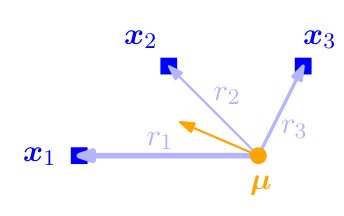
\includegraphics[width=0.92\textwidth,keepaspectratio]{docs/images/Figure11.4.png}
\caption*{图 11.4}
\end{figure}


直观上，均值 $ \boldsymbol{\mu}_k $ 会被数据点 $ \boldsymbol{x}_n $ 拉向责任度较高的方向。将第 $ k $ 个分量的责任度归一化为概率向量：

\begin{equation}
\boldsymbol{r}_k := [r_{1k}, \ldots, r_{Nk}]^\top / N_k .
\tag{11.25}
\end{equation}

则均值更新也可以写成在该责任度分布下对数据的期望：

\begin{equation}
\boldsymbol{\mu}_k \leftarrow \mathbb{E}_{\boldsymbol{r}_k}[\boldsymbol{X}] .
\tag{11.26}
\end{equation}

\begin{notebox}
\textbf{例 11.3（均值参数更新）}
\end{notebox}

\begin{notebox}
图 11.5 展示了在图 11.3 的初始设定下，仅执行一次均值更新（保持方差和混合权重不变）的前后对比。我们看到，分量 1 和分量 3 的中心迅速朝向数据密集区域移动。
\end{notebox}


\begin{figure}[H]
\centering
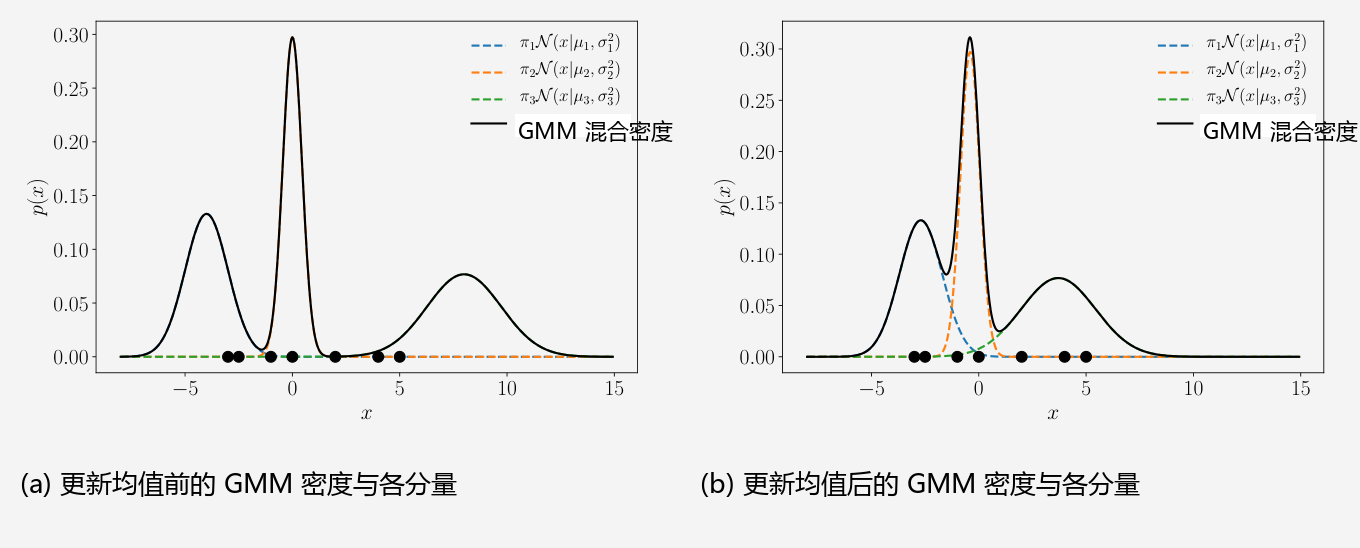
\includegraphics[width=0.92\textwidth,keepaspectratio]{docs/images/Figure11.5.png}
\caption*{图 11.5}
\end{figure}


在图 11.3 的示例中，均值更新如下：

\begin{equation}
\mu_1: -4 \to -2.7 .
\tag{11.27}
\end{equation}

\begin{equation}
\mu_2: 0 \to -0.4 .
\tag{11.28}
\end{equation}

\begin{equation}
\mu_3: 8 \to 3.7 .
\tag{11.29}
\end{equation}

可以看到，第一个和第三个混合分量的均值向数据所在区域移动，而第二个分量的均值变化并不明显。

\medskip\hrule\medskip

\section*{11.2.3 更新协方差矩阵}
\addcontentsline{toc}{subsection}{11.2.3 更新协方差矩阵}

\textbf{定理 11.2（GMM 协方差更新法则）}。高斯混合模型协方差矩阵参数 $ \boldsymbol{\Sigma}_k $（$ k = 1, \ldots, K $）的更新公式为：

\begin{equation}
\boldsymbol{\Sigma}_k^{\text{new}} = \frac{1}{N_k}\sum_{n=1}^N r_{nk}(\boldsymbol{x}_n - \boldsymbol{\mu}_k)(\boldsymbol{x}_n - \boldsymbol{\mu}_k)^\top .
\tag{11.30}
\end{equation}

*证明*。 根据多元求导法则计算 $ \mathcal{L} $ 关于矩阵 $ \boldsymbol{\Sigma}_k $ 的偏导数：

\begin{equation}
\begin{adjustbox}{max width=\linewidth}
\frac{\partial \mathcal{L}}{\partial \boldsymbol{\Sigma}_k} = \sum_{n=1}^N \frac{1}{p(\boldsymbol{x}_n \mid \boldsymbol{\theta})}\frac{\partial p(\boldsymbol{x}_n \mid \boldsymbol{\theta})}{\partial \boldsymbol{\Sigma}_k} .
\end{adjustbox}
\tag{11.31}
\end{equation}

由高斯分布关于协方差矩阵的求导公式（式 (5.101) 与 (5.106)）：

只保留混合密度中依赖于第 $ k $ 个协方差矩阵的项，可得：

\begin{equation}
\begin{adjustbox}{max width=\linewidth}
\frac{\partial p(\boldsymbol{x}_n \mid \boldsymbol{\theta})}{\partial \boldsymbol{\Sigma}_k} = \frac{\partial}{\partial \boldsymbol{\Sigma}_k} \left[ \pi_k (2\pi)^{-\frac{D}{2}} \det(\boldsymbol{\Sigma}_k)^{-\frac{1}{2}} \exp\left( -\frac{1}{2}(\boldsymbol{x}_n - \boldsymbol{\mu}_k)^\top \boldsymbol{\Sigma}_k^{-1}(\boldsymbol{x}_n - \boldsymbol{\mu}_k) \right) \right] .
\end{adjustbox}
\tag{11.32a}
\end{equation}

\begin{equation}
\begin{adjustbox}{max width=\linewidth}
= \pi_k (2\pi)^{-\frac{D}{2}} \left[ \frac{\partial}{\partial \boldsymbol{\Sigma}_k}\det(\boldsymbol{\Sigma}_k)^{-\frac{1}{2}} \exp\left( -\frac{1}{2}(\boldsymbol{x}_n - \boldsymbol{\mu}_k)^\top \boldsymbol{\Sigma}_k^{-1}(\boldsymbol{x}_n - \boldsymbol{\mu}_k) \right)
\right.
\end{adjustbox}
\tag{11.32b}
\end{equation}

\begin{equation}
\begin{adjustbox}{max width=\linewidth}
\left. \qquad + \det(\boldsymbol{\Sigma}_k)^{-\frac{1}{2}} \frac{\partial}{\partial \boldsymbol{\Sigma}_k} \exp\left( -\frac{1}{2}(\boldsymbol{x}_n - \boldsymbol{\mu}_k)^\top \boldsymbol{\Sigma}_k^{-1}(\boldsymbol{x}_n - \boldsymbol{\mu}_k) \right) \right] .
\end{adjustbox}
\tag{11.32c}
\end{equation}

现在使用以下两个矩阵求导恒等式：

\begin{equation}
\frac{\partial}{\partial \boldsymbol{\Sigma}_k}\det(\boldsymbol{\Sigma}_k)^{-\frac{1}{2}} = -\frac{1}{2}\det(\boldsymbol{\Sigma}_k)^{-\frac{1}{2}}\boldsymbol{\Sigma}_k^{-1}
\tag{11.33}
\end{equation}

\begin{equation}
\begin{adjustbox}{max width=\linewidth}
\frac{\partial}{\partial \boldsymbol{\Sigma}_k}\left[ (\boldsymbol{x}_n - \boldsymbol{\mu}_k)^\top \boldsymbol{\Sigma}_k^{-1}(\boldsymbol{x}_n - \boldsymbol{\mu}_k) \right] = -\boldsymbol{\Sigma}_k^{-1}(\boldsymbol{x}_n - \boldsymbol{\mu}_k)(\boldsymbol{x}_n - \boldsymbol{\mu}_k)^\top \boldsymbol{\Sigma}_k^{-1} .
\end{adjustbox}
\tag{11.34}
\end{equation}

整理后可得：

\begin{equation}
\begin{adjustbox}{max width=\linewidth}
\frac{\partial p(\boldsymbol{x}_n \mid \boldsymbol{\theta})}{\partial \boldsymbol{\Sigma}_k} = \pi_k \mathcal{N}\left(\boldsymbol{x}_n \mid \boldsymbol{\mu}_k, \boldsymbol{\Sigma}_k\right) \left[ -\frac{1}{2}\left( \boldsymbol{\Sigma}_k^{-1} - \boldsymbol{\Sigma}_k^{-1}(\boldsymbol{x}_n - \boldsymbol{\mu}_k)(\boldsymbol{x}_n - \boldsymbol{\mu}_k)^\top \boldsymbol{\Sigma}_k^{-1} \right) \right] .
\end{adjustbox}
\tag{11.35}
\end{equation}

将式 (11.35) 代入式 (11.31) 中并利用责任度 $ r_{nk} $ 的定义：

\begin{equation}
\begin{adjustbox}{max width=\linewidth}
\frac{\partial \mathcal{L}}{\partial \boldsymbol{\Sigma}_k} = \sum_{n=1}^N \frac{\partial \log p(\boldsymbol{x}_n \mid \boldsymbol{\theta})}{\partial \boldsymbol{\Sigma}_k} = \sum_{n=1}^N \frac{1}{p(\boldsymbol{x}_n \mid \boldsymbol{\theta})}\frac{\partial p(\boldsymbol{x}_n \mid \boldsymbol{\theta})}{\partial \boldsymbol{\Sigma}_k} .
\end{adjustbox}
\tag{11.36a}
\end{equation}

\begin{equation}
\begin{adjustbox}{max width=\linewidth}
= \sum_{n=1}^N \underbrace{\frac{\pi_k \mathcal{N}(\boldsymbol{x}_n \mid \boldsymbol{\mu}_k, \boldsymbol{\Sigma}_k)}{\sum_{j=1}^K \pi_j \mathcal{N}(\boldsymbol{x}_n \mid \boldsymbol{\mu}_j, \boldsymbol{\Sigma}_j)}}_{= r_{nk}} \left[-\frac{1}{2}\left(\boldsymbol{\Sigma}_k^{-1} - \boldsymbol{\Sigma}_k^{-1}(\boldsymbol{x}_n - \boldsymbol{\mu}_k)(\boldsymbol{x}_n - \boldsymbol{\mu}_k)^\top \boldsymbol{\Sigma}_k^{-1}\right)\right] .
\end{adjustbox}
\tag{11.36b}
\end{equation}

\begin{equation}
= -\frac{1}{2}\sum_{n=1}^N r_{nk}\left(\boldsymbol{\Sigma}_k^{-1} - \boldsymbol{\Sigma}_k^{-1}(\boldsymbol{x}_n - \boldsymbol{\mu}_k)(\boldsymbol{x}_n - \boldsymbol{\mu}_k)^\top \boldsymbol{\Sigma}_k^{-1}\right)
\tag{11.36c}
\end{equation}

\begin{equation}
\begin{adjustbox}{max width=\linewidth}
= -\frac{1}{2}\boldsymbol{\Sigma}_k^{-1}\sum_{n=1}^N r_{nk} + \frac{1}{2}\boldsymbol{\Sigma}_k^{-1}\left( \sum_{n=1}^N r_{nk}(\boldsymbol{x}_n - \boldsymbol{\mu}_k)(\boldsymbol{x}_n - \boldsymbol{\mu}_k)^\top \right)\boldsymbol{\Sigma}_k^{-1} .
\end{adjustbox}
\tag{11.36d}
\end{equation}

令该偏导数为 $ \boldsymbol{0} $，得到如下必要最优性条件：

\begin{equation}
N_k\boldsymbol{\Sigma}_k^{-1} = \boldsymbol{\Sigma}_k^{-1}\left(\sum_{n=1}^N r_{nk}(\boldsymbol{x}_n - \boldsymbol{\mu}_k)(\boldsymbol{x}_n - \boldsymbol{\mu}_k)^\top\right)\boldsymbol{\Sigma}_k^{-1}
\tag{11.37a}
\end{equation}

\begin{equation}
N_k\boldsymbol{I} = \left(\sum_{n=1}^N r_{nk}(\boldsymbol{x}_n - \boldsymbol{\mu}_k)(\boldsymbol{x}_n - \boldsymbol{\mu}_k)^\top\right)\boldsymbol{\Sigma}_k^{-1} .
\tag{11.37b}
\end{equation}

解出 $ \boldsymbol{\Sigma}_k $，即得定理 11.2 的更新公式：

\begin{equation}
\boldsymbol{\Sigma}_k^{\text{new}} = \frac{1}{N_k}\sum_{n=1}^N r_{nk}(\boldsymbol{x}_n - \boldsymbol{\mu}_k)(\boldsymbol{x}_n - \boldsymbol{\mu}_k)^\top .
\tag{11.38}
\end{equation}

证毕。

类似于均值更新，协方差矩阵的更新同样是基于中心化残差平方外积的重要性加权估计。

\begin{notebox}
\textbf{例 11.4（方差参数更新）}
\end{notebox}

\begin{notebox}
在图 11.3 的示例中，执行方差更新后，三个分量的方差分别更新为：
\end{notebox}

\begin{notebox}
\begin{equation}
\sigma_1^2: 1 \to 0.14 .
\tag{11.39}
\end{equation}
\end{notebox}

\begin{notebox}
\begin{equation}
\sigma_2^2: 0.2 \to 0.44 .
\tag{11.40}
\end{equation}
\end{notebox}

\begin{notebox}
\begin{equation}
\sigma_3^2: 3 \to 1.53 .
\tag{11.41}
\end{equation}
\end{notebox}

\begin{notebox}
图 11.6 对比了更新方差前后的 GMM 密度变化。我们发现分量 1 和分量 3 的方差显著收缩，使得概率峰值更加锐利地吻合局部数据簇。
\end{notebox}


\begin{figure}[H]
\centering
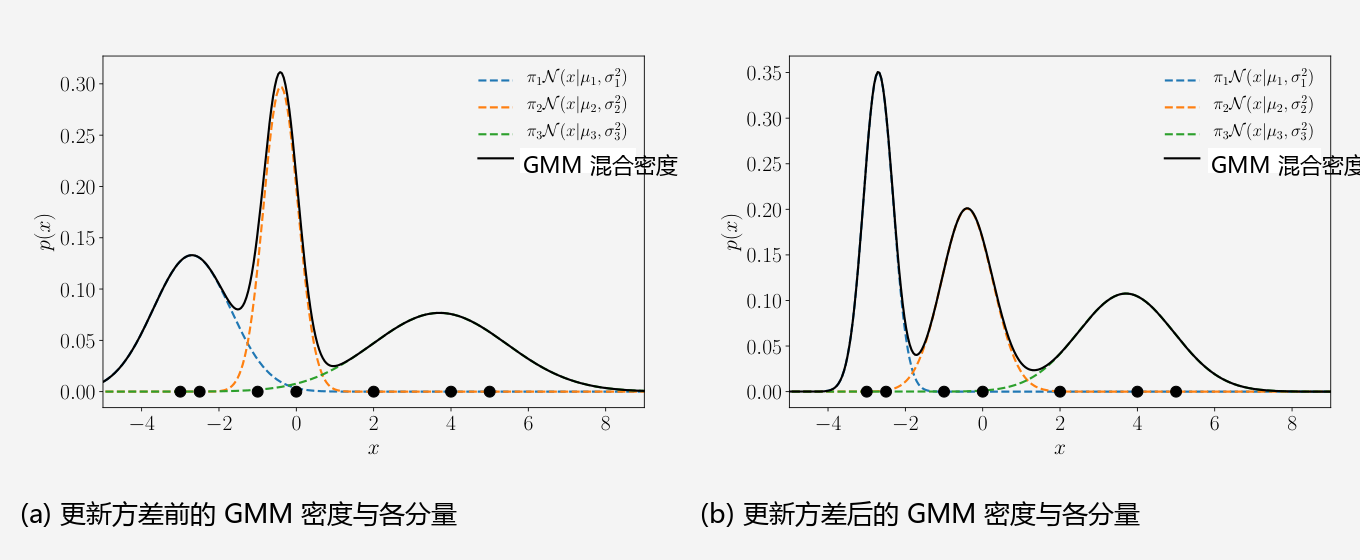
\includegraphics[width=0.92\textwidth,keepaspectratio]{docs/images/Figure11.6.png}
\caption*{图 11.6}
\end{figure}


\medskip\hrule\medskip

\section*{11.2.4 更新混合权重}
\addcontentsline{toc}{subsection}{11.2.4 更新混合权重}

\textbf{定理 11.3（GMM 权重更新法则）}。高斯混合模型权重参数 $ \pi_k $（$ k = 1, \ldots, K $）的更新公式为：

\begin{equation}
\pi_k^{\text{new}} = \frac{N_k}{N}
\tag{11.42}
\end{equation}

其中 $ N $ 为总数据点数量，$ N_k $ 为式 (11.24) 定义的总责任度。

*证明*。 由于混合权重必须满足等式约束 $ \sum_{k=1}^K \pi_k = 1 $，我们利用拉格朗日乘子法构建拉格朗日函数：

\begin{equation}
\mathcal{L}_{\pi} = \mathcal{L} + \lambda \left( \sum_{k=1}^K \pi_k - 1 \right) .
\tag{11.43a}
\end{equation}

\begin{equation}
= \sum_{n=1}^N \log \left( \sum_{k=1}^K \pi_k \mathcal{N}\left(\boldsymbol{x}_n \mid \boldsymbol{\mu}_k, \boldsymbol{\Sigma}_k\right) \right) + \lambda \left( \sum_{k=1}^K \pi_k - 1 \right) .
\tag{11.43b}
\end{equation}

关于 $ \pi_k $ 求偏导数：

\begin{equation}
\begin{adjustbox}{max width=\linewidth}
\frac{\partial \mathcal{L}_{\pi}}{\partial \pi_k} = \sum_{n=1}^N \frac{\mathcal{N}\left(\boldsymbol{x}_n \mid \boldsymbol{\mu}_k, \boldsymbol{\Sigma}_k\right)}{\sum_{j=1}^K \pi_j \mathcal{N}\left(\boldsymbol{x}_n \mid \boldsymbol{\mu}_j, \boldsymbol{\Sigma}_j\right)} + \lambda .
\end{adjustbox}
\tag{11.44a}
\end{equation}

\begin{equation}
\begin{adjustbox}{max width=\linewidth}
= \frac{1}{\pi_k}\sum_{n=1}^N \underbrace{\frac{\pi_k \mathcal{N}\left(\boldsymbol{x}_n \mid \boldsymbol{\mu}_k, \boldsymbol{\Sigma}_k\right)}{\sum_{j=1}^K \pi_j \mathcal{N}\left(\boldsymbol{x}_n \mid \boldsymbol{\mu}_j, \boldsymbol{\Sigma}_j\right)}}_{=r_{nk}} + \lambda = \frac{N_k}{\pi_k} + \lambda .
\end{adjustbox}
\tag{11.44b}
\end{equation}

此外，关于拉格朗日乘子 $ \lambda $ 的偏导数为：

\begin{equation}
\frac{\partial \mathcal{L}_{\pi}}{\partial \lambda} = \sum_{k=1}^K \pi_k - 1 .
\tag{11.45}
\end{equation}

令这两个偏导数为 0，得到方程组：

\begin{equation}
\pi_k = -\frac{N_k}{\lambda} .
\tag{11.46}
\end{equation}

\begin{equation}
\sum_{k=1}^K \pi_k = 1 .
\tag{11.47}
\end{equation}

将式 (11.46) 代入式 (11.47) 并求解 $ \lambda $：

\begin{equation}
\sum_{k=1}^K \pi_k = -\frac{1}{\lambda}\sum_{k=1}^K N_k = -\frac{N}{\lambda} = 1 \iff \lambda = -N .
\tag{11.48}
\end{equation}

将 $ \lambda = -N $ 带回，立即得出：

\begin{equation}
\pi_k^{\text{new}} = \frac{N_k}{N} .
\tag{11.49}
\end{equation}

证毕。

式 (11.42) 直观地将混合权重解释为第 $ k $ 个簇的总责任度占全部数据点总容量的比例，即第 $ k $ 个分量对整个数据集的相对重要性。

\begin{notebox}
\textbf{例 11.5（混合权重更新）}
\end{notebox}

\begin{notebox}
在我们的示例中，混合权重从均匀分布 $ \pi_k = \frac{1}{3} \approx 0.33 $ 更新为：
\end{notebox}

\begin{notebox}
\begin{equation}
\pi_1: \frac{1}{3} \to 0.29 .
\tag{11.50}
\end{equation}
\end{notebox}

\begin{notebox}
\begin{equation}
\pi_2: \frac{1}{3} \to 0.29 .
\tag{11.51}
\end{equation}
\end{notebox}

\begin{notebox}
\begin{equation}
\pi_3: \frac{1}{3} \to 0.42 .
\tag{11.52}
\end{equation}
\end{notebox}

\begin{notebox}
图 11.7 展示了更新混合权重前后的 GMM 密度变化。
\end{notebox}


\begin{figure}[H]
\centering
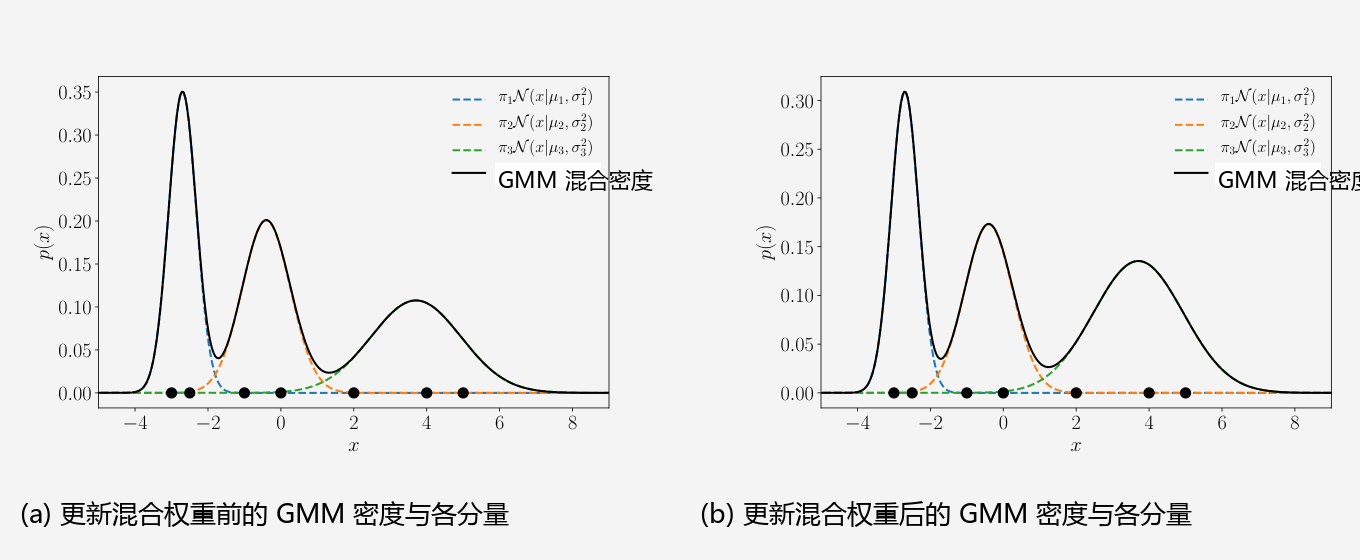
\includegraphics[width=0.92\textwidth,keepaspectratio]{docs/images/Figure11.7.png}
\caption*{图 11.7}
\end{figure}


\section*{11.3 期望最大化算法}
\addcontentsline{toc}{section}{11.3 期望最大化算法}
\label{sec:11.3}

\emph{期望最大化（expectation maximization, EM）} 算法由 Dempster et al. (1977) 提出，是一种用于在混合模型以及更一般的含有不可观测隐变量的模型中学习参数（极大似然或 MAP 估计）的通用迭代优化框架。

在我们考虑的高斯混合模型中，我们首先为模型参数 $ \boldsymbol{\mu}_k, \boldsymbol{\Sigma}_k, \pi_k $ 设定初始值，并在以下两个步骤之间交替迭代直至收敛：

\begin{itemize}
\item \textbf{E 步（期望步，Expectation step）}：利用当前参数评估所有数据点关于各个混合分量的后验责任度 $ r_{nk} $（即第 $ n $ 个数据点属于第 $ k $ 个混合分量的后验概率）；
\item \textbf{M 步（最大化步，Maximization step）}：利用最新计算的责任度重新估计并更新模型参数 $ \boldsymbol{\mu}_k, \boldsymbol{\Sigma}_k, \pi_k $。
\end{itemize}

Neal and Hinton (1999) 证明，EM 算法的每一次迭代都保证能使对数似然函数单调非递减。在实际工程实现中，我们可以通过监测对数似然的增量或参数矢量的改变量来判断算法是否收敛。

用于估计 GMM 参数的 EM 算法标准具体执行流程如下：

\begin{enumerate}
\item \textbf{初始化}：初始化均值 $ \boldsymbol{\mu}_k $、协方差矩阵 $ \boldsymbol{\Sigma}_k $ 和混合权重 $ \pi_k $（例如利用 $ K $-means 聚类中心初始化均值，样本全局协方差初始化 $ \boldsymbol{\Sigma}_k $，均匀分布初始化 $ \pi_k = \frac{1}{K} $）；
\item \textbf{E 步}：利用当前参数值 $ \pi_k, \boldsymbol{\mu}_k, \boldsymbol{\Sigma}_k $，为每个数据点 $ \boldsymbol{x}_n $ 评估其关于各个分量的责任度 $ r_{nk} $：
\end{enumerate}

\begin{equation}
r_{nk} = \frac{\pi_k \mathcal{N}\left(\boldsymbol{x}_n \mid \boldsymbol{\mu}_k, \boldsymbol{\Sigma}_k\right)}{\sum_{j=1}^K \pi_j \mathcal{N}\left(\boldsymbol{x}_n \mid \boldsymbol{\mu}_j, \boldsymbol{\Sigma}_j\right)} ;
\tag{11.53}
\end{equation}

\begin{enumerate}
\item \textbf{M 步}：利用 E 步求得的最新责任度 $ r_{nk} $，重新估计并更新模型参数：
\end{enumerate}

\begin{equation}
\boldsymbol{\mu}_k = \frac{1}{N_k}\sum_{n=1}^N r_{nk}\boldsymbol{x}_n
\tag{11.54}
\end{equation}

\begin{equation}
\boldsymbol{\Sigma}_k = \frac{1}{N_k}\sum_{n=1}^N r_{nk}(\boldsymbol{x}_n - \boldsymbol{\mu}_k)(\boldsymbol{x}_n - \boldsymbol{\mu}_k)^\top
\tag{11.55}
\end{equation}

\begin{equation}
\pi_k = \frac{N_k}{N}
\tag{11.56}
\end{equation}

其中 $ N_k := \sum_{n=1}^N r_{nk} $ 为第 $ k $ 个分量的有效总责任度；

\begin{enumerate}
\item \textbf{收敛检验}：评估对数似然 $ \mathcal{L} $，若对数似然的变化量小于预设容差或达到最大迭代轮数，则终止算法；否则返回第 2 步继续迭代。
\end{enumerate}

\begin{notebox}
\textbf{例 11.6（GMM 拟合实例）}
\end{notebox}

\begin{notebox}
将 EM 算法应用于图 11.3 中的一维数据集。在经历了仅仅 5 轮迭代后，EM 算法便完全收敛。图 11.8(a) 展示了最终收敛的 GMM 拟合分布，图 11.8(b) 展示了负对数似然随 EM 迭代轮数单调下降的平滑曲线。最终求得的 GMM 参数分布为：
\end{notebox}

\begin{notebox}
\begin{equation}
p(x) = 0.29\mathcal{N}(x \mid -2.75, 0.06) + 0.28\mathcal{N}(x \mid -0.50, 0.25) + 0.43\mathcal{N}(x \mid 3.64, 1.63) .
\tag{11.57}
\end{equation}
\end{notebox}


\begin{figure}[H]
\centering
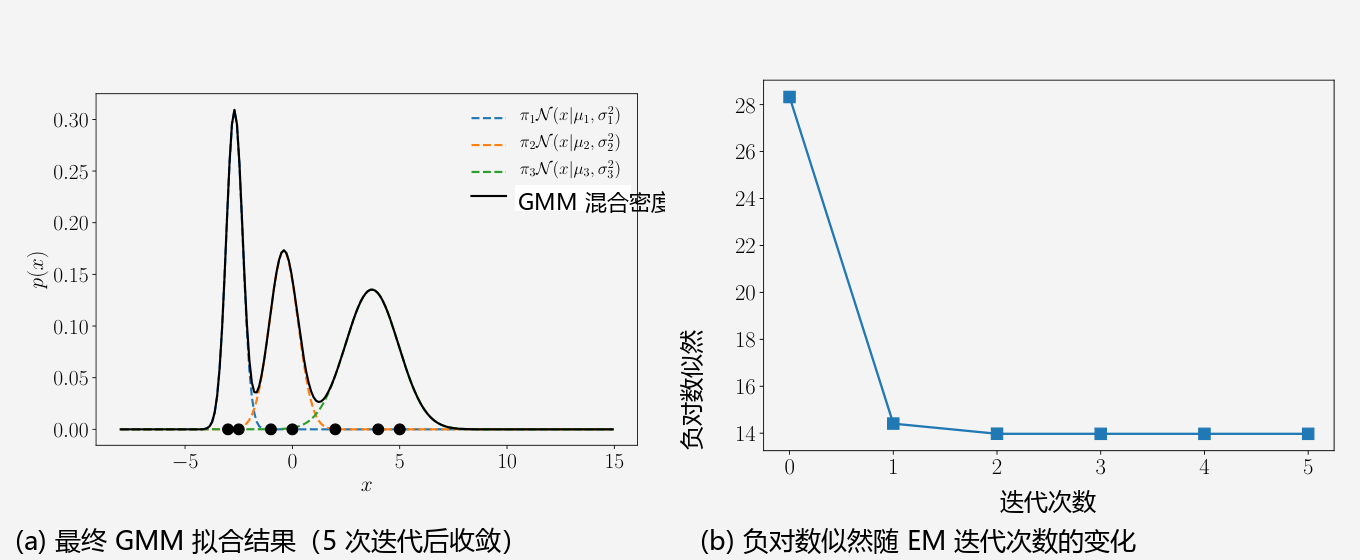
\includegraphics[width=0.92\textwidth,keepaspectratio]{docs/images/Figure11.8.png}
\caption*{图 11.8}
\end{figure}


接下来，我们将 EM 算法应用于图 11.1 所示的复杂二维非高斯数据集，设定混合分量个数 $ K = 3 $。图 11.9 完整可视化了 EM 算法的迭代演进历程：

\begin{itemize}
\item 图 11.9(a) 为原始输入数据；
\item 图 11.9(b) 展示了负对数似然随迭代轮数的急剧下降；
\item 图 11.9(c)–(f) 分别展示了算法在初始化、第 1 轮、第 10 轮以及第 62 轮迭代收敛时的各个高斯椭圆等高线与均值中心（黄色实心圆）。
\end{itemize}


\begin{figure}[H]
\centering
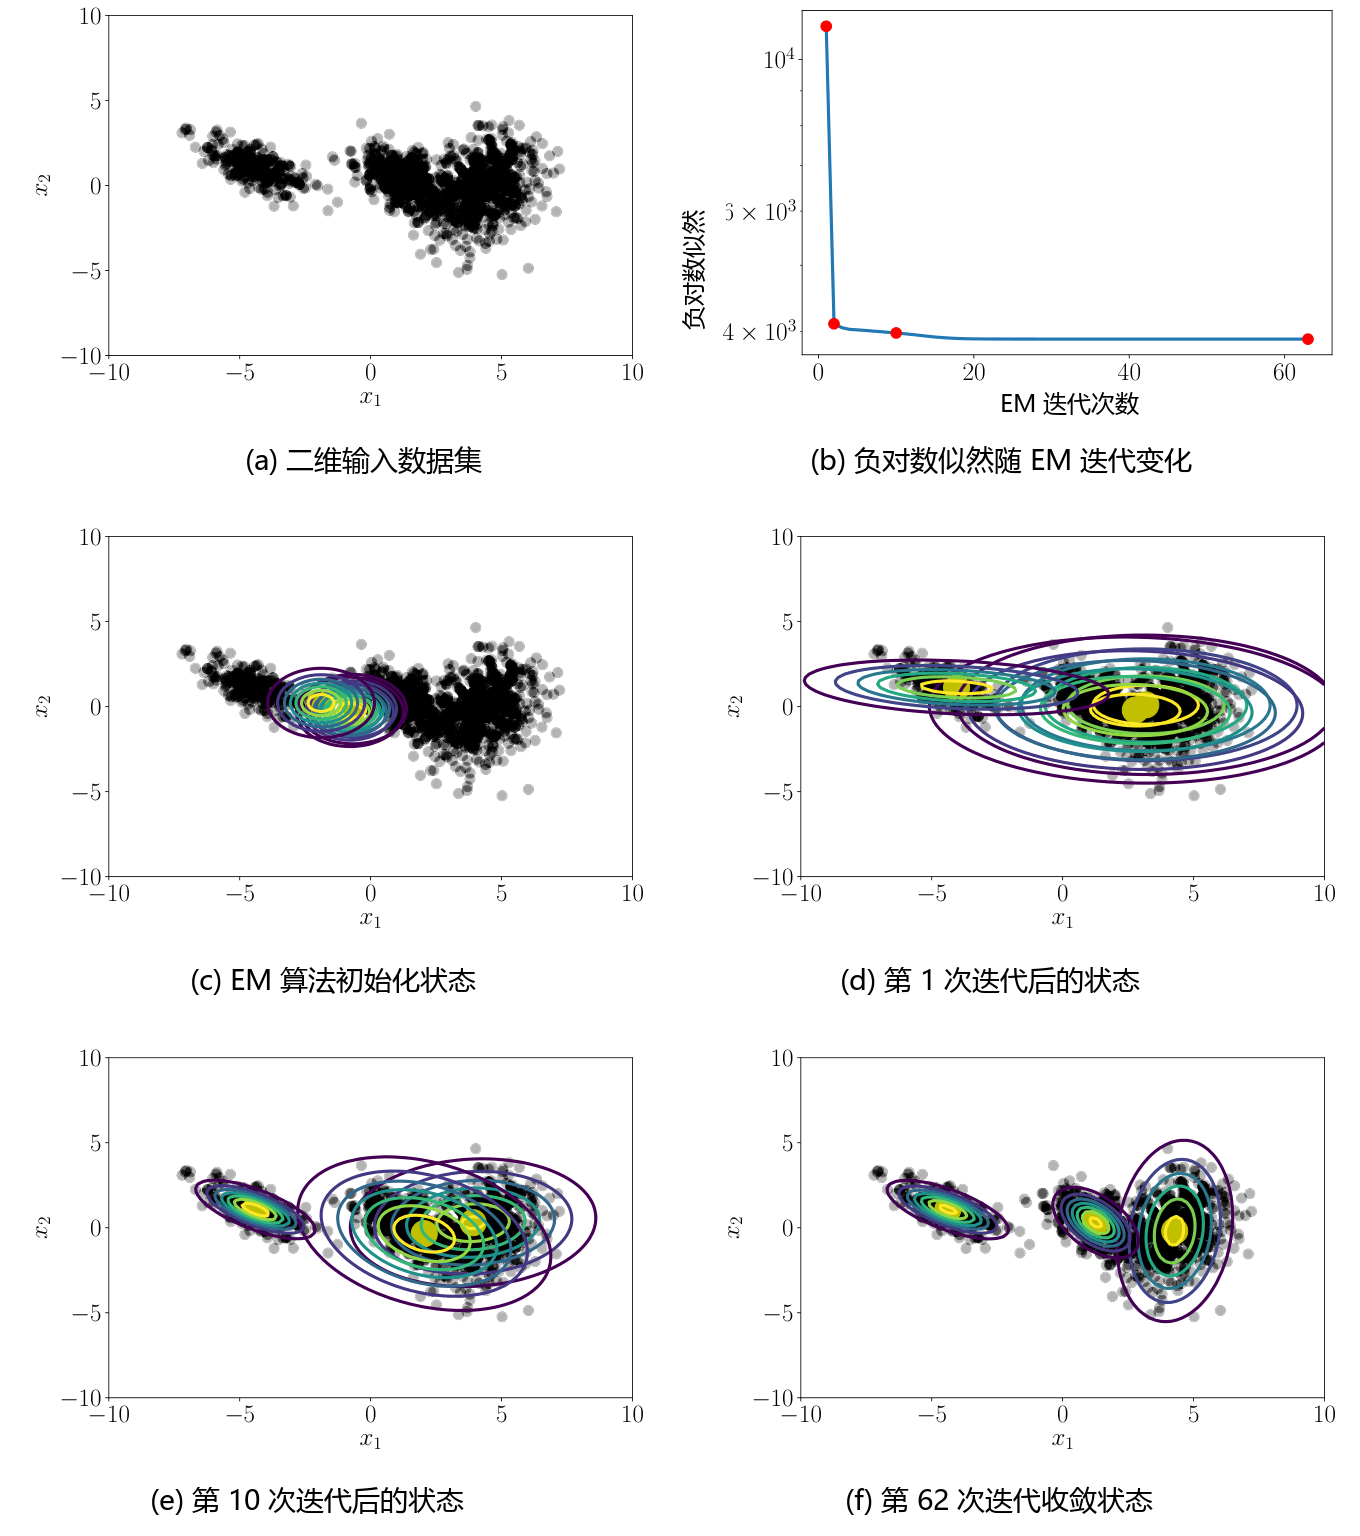
\includegraphics[width=320pt,keepaspectratio]{docs/images/Figure11.9.png}
\caption*{图 11.9}
\end{figure}


图 11.10(a) 展示了最终收敛的 GMM 密度等高线；图 11.10(b) 根据收敛后各个混合分量对数据点的后验责任度 $ r_{nk} $ 对数据点进行了软聚类着色。左侧独立簇被单一分量以几乎 100\% 的确定性清晰覆盖；而右侧相互重叠交织的两个数据簇则处于中间模糊地带，交界处的样本点无法被非黑即白地硬划分给某一个簇，其责任度平滑分布在 0.5 左右，完美展现了概率软聚类的优势。


\begin{figure}[H]
\centering
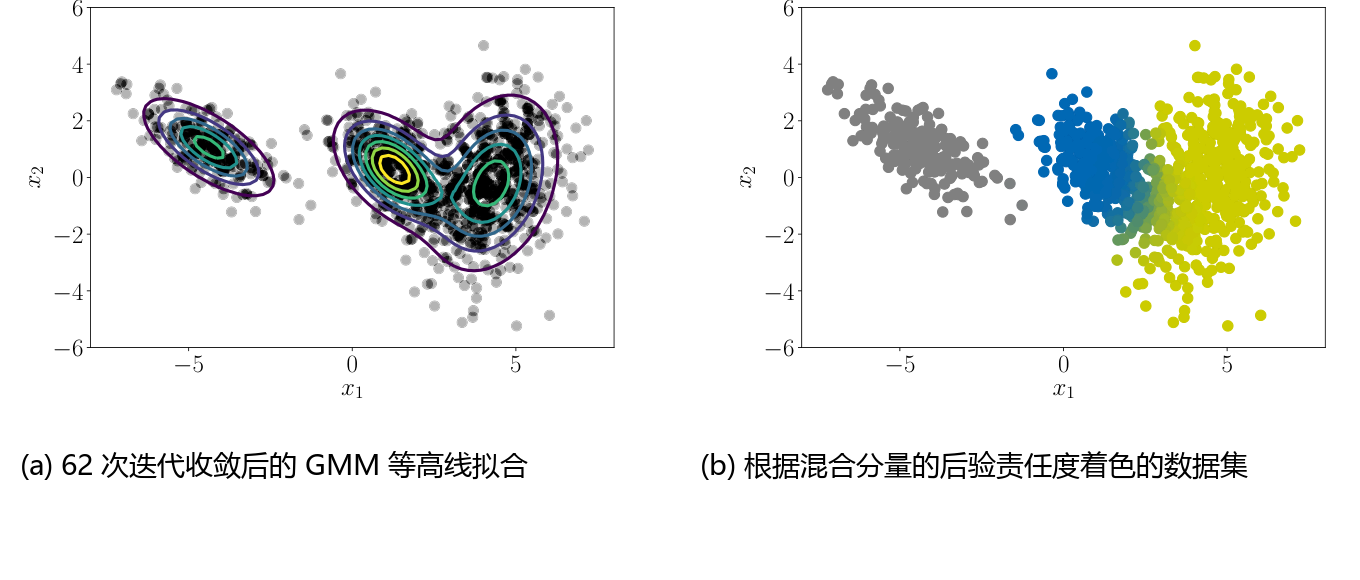
\includegraphics[width=0.92\textwidth,keepaspectratio]{docs/images/Figure11.10.png}
\caption*{图 11.10}
\end{figure}


\section*{11.4 隐变量视角}
\addcontentsline{toc}{section}{11.4 隐变量视角}
\label{sec:11.4}

我们可以从离散 \emph{隐变量模型（latent-variable model）} 的视角来重新审视高斯混合模型，即隐变量 $ \boldsymbol{z} $ 仅能在一组离散的可能取值中选择其一。这与第 10 章的 PCA 形成了鲜明的对比——在 PCA 中，隐变量是生活在 $ \mathbb{R}^M $ 中的连续型数值向量。

采用概率隐变量视角具有如下显著优势：

\begin{enumerate}
\item 它为我们在前面小节中做出的启发式直觉决定提供了坚实严谨的数学辩护；
\item 它允许将“责任度”严格且具体地解释为隐变量状态的后验概率分布；
\item 更新模型参数的迭代算法可以被完全原则性地推导为隐变量模型极大似然估计的标准 EM 算法。
\end{enumerate}

\medskip\hrule\medskip

\section*{11.4.1 生成过程与概率模型}
\addcontentsline{toc}{subsection}{11.4.1 生成过程与概率模型}

为了推导 GMM 的概率图模型，思考基于概率模型的数据生成过程是非常有启发性的。

我们假设一个包含 $ K $ 个分量的混合模型，并且每一个具体的观测数据点 $ \boldsymbol{x} $ 都是由其中恰好一个混合分量生成的。我们引入一个二元指示变量 $ z_k \in \{0, 1\} $（具有两个状态，见 6.2 节），用以指示第 $ k $ 个混合分量是否生成了该数据点，即：

\begin{equation}
p(\boldsymbol{x} \mid z_k = 1) = \mathcal{N}\left(\boldsymbol{x} \mid \boldsymbol{\mu}_k, \boldsymbol{\Sigma}_k\right) .
\tag{11.58}
\end{equation}

我们将 $ \boldsymbol{z} := [z_1, \ldots, z_K]^\top \in \{0, 1\}^K $ 定义为一个状态向量，其中包含 $ K-1 $ 个 0 和恰好一个 1。例如，当 $ K = 3 $ 时，一个合法的 $ \boldsymbol{z} $ 可以是 $ \boldsymbol{z} = [0, 1, 0]^\top $，由于 $ z_2 = 1 $，这代表选中了第二个混合分量。

\emph{备注} 。这类概率分布有时被称为“多元伯努利分布”（Multinoulli），它是伯努利分布在二元以上分类变量上的自然推广（Murphy, 2012）。

指示向量 $ \boldsymbol{z} $ 的性质意味着 $ \sum_{k=1}^K z_k = 1 $。因此，$ \boldsymbol{z} $ 是一个 \emph{独热编码（one-hot encoding）} （亦称 1-of-$ K $ 表示）。

到目前为止，我们假设指示变量 $ z_k $ 是已知的。然而在无监督学习实践中，真实生成类别是完全不可见的隐变量。因此，我们在隐变量 $ \boldsymbol{z} $ 上引入一个先验分布：

\begin{equation}
p(\boldsymbol{z}) = \boldsymbol{\pi} = [\pi_1, \ldots, \pi_K]^\top , \quad \sum_{k=1}^K \pi_k = 1
\tag{11.59}
\end{equation}

该概率向量的第 $ k $ 个分量

\begin{equation}
\pi_k = p(z_k = 1)
\tag{11.60}
\end{equation}

精确描述了第 $ k $ 个混合分量生成任意数据点 $ \boldsymbol{x} $ 的先验概率。


\begin{figure}[H]
\centering
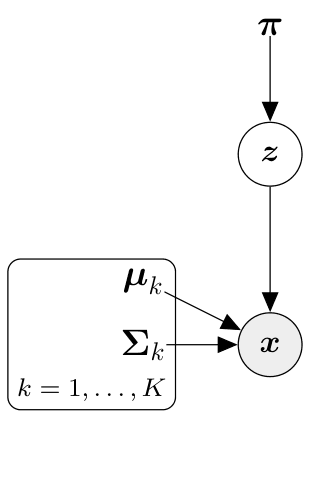
\includegraphics[width=0.84\textwidth,height=0.80\textheight,keepaspectratio]{docs/images/Figure11.11.png}
\caption*{图 11.11}
\end{figure}


\emph{备注} （从 GMM 中采样数据） 。该隐变量模型的结构（对应图 11.11 的概率图模型）支持一种极其自然的先祖采样（ancestral sampling）数据生成流程：

\begin{enumerate}
\item 采样潜在类别：$ \boldsymbol{z}^{(i)} \sim p(\boldsymbol{z}) $；
\item 采样连续观测：$ \boldsymbol{x}^{(i)} \sim p(\boldsymbol{x} \mid \boldsymbol{z}^{(i)} = 1) $。
\end{enumerate}

第一步，我们依据先验概率向量 $ \boldsymbol{\pi} $ 随机抽取一个分量索引 $ k $（通过独热编码 $ \boldsymbol{z} $ 表示）；第二步，从对应的第 $ k $ 个高斯分量中抽取高斯连续样本。当我们随后丢弃不可见的隐变量标签时，所留下的 $ \{\boldsymbol{x}^{(i)}\} $ 便是来自 GMM 的纯正无偏样本。

一般而言，概率模型由观测数据与隐变量的联合分布唯一定义（见 8.4 节）。利用式 (11.59)–(11.60) 中的先验 $ p(\boldsymbol{z}) $ 以及式 (11.58) 中的条件分布 $ p(\boldsymbol{x} \mid \boldsymbol{z}) $，该联合分布的全部 $ K $ 个离散分量由下式给出：

\begin{equation}
p(\boldsymbol{x}, z_k = 1) = p(\boldsymbol{x} \mid z_k = 1)p(z_k = 1) = \pi_k \mathcal{N}\left(\boldsymbol{x} \mid \boldsymbol{\mu}_k, \boldsymbol{\Sigma}_k\right)
\tag{11.61}
\end{equation}

由此完全确定了 GMM 的完整概率联合分布：

\begin{equation}
\begin{adjustbox}{max width=\linewidth}
p(\boldsymbol{x}, \boldsymbol{z}) = \begin{bmatrix} p(\boldsymbol{x}, z_1 = 1) \\ \vdots \\ p(\boldsymbol{x}, z_K = 1) \end{bmatrix} = \begin{bmatrix} \pi_1 \mathcal{N}(\boldsymbol{x} \mid \boldsymbol{\mu}_1, \boldsymbol{\Sigma}_1) \\ \vdots \\ \pi_K \mathcal{N}(\boldsymbol{x} \mid \boldsymbol{\mu}_K, \boldsymbol{\Sigma}_K) \end{bmatrix} .
\end{adjustbox}
\tag{11.62}
\end{equation}

\medskip\hrule\medskip

\section*{11.4.2 似然函数}
\addcontentsline{toc}{subsection}{11.4.2 似然函数}

为了在隐变量模型中获得边际似然 $ p(\boldsymbol{x} \mid \boldsymbol{\theta}) $，我们需要将不可观测的隐变量 $ \boldsymbol{z} $ 边缘化消去（见 8.4.3 节）。在我们的离散设定下，这通过对联合分布 (11.62) 关于 $ \boldsymbol{z} $ 的所有可能状态求和来实现：

\begin{equation}
p(\boldsymbol{x} \mid \boldsymbol{\theta}) = \sum_{\boldsymbol{z}} p(\boldsymbol{x} \mid \boldsymbol{\theta}, \boldsymbol{z})p(\boldsymbol{z} \mid \boldsymbol{\theta})
\tag{11.63}
\end{equation}

其中 $ \boldsymbol{\theta} := \{\boldsymbol{\mu}_k, \boldsymbol{\Sigma}_k, \pi_k : k = 1, \ldots, K\} $。由于每个独热向量 $ \boldsymbol{z} $ 中只有一个非零分量 1，$ \boldsymbol{z} $ 一共只有 $ K $ 种可能的状态配置。因此，关于所有可能独热配置的求和等价于关于分量索引 $ k $ 的有限求和：

例如，当 $ K = 3 $ 时，$ \boldsymbol{z} $ 的三种可能配置为：

\begin{equation}
\begin{bmatrix} 1 \\ 0 \\ 0 \end{bmatrix}, \quad
\begin{bmatrix} 0 \\ 1 \\ 0 \end{bmatrix}, \quad
\begin{bmatrix} 0 \\ 0 \\ 1 \end{bmatrix} .
\tag{11.64}
\end{equation}

将所有可能配置代入式 (11.63)，可得：

\begin{equation}
p(\boldsymbol{x} \mid \boldsymbol{\theta}) = \sum_{\boldsymbol{z}} p(\boldsymbol{x} \mid \boldsymbol{\theta}, \boldsymbol{z})p(\boldsymbol{z} \mid \boldsymbol{\theta}) .
\tag{11.65a}
\end{equation}

\begin{equation}
= \sum_{k=1}^K p(\boldsymbol{x} \mid \boldsymbol{\theta}, z_k = 1)p(z_k = 1 \mid \boldsymbol{\theta}) .
\tag{11.65b}
\end{equation}

\begin{equation}
p(\boldsymbol{x} \mid \boldsymbol{\theta}) = \sum_{k=1}^K p(\boldsymbol{x} \mid \boldsymbol{\theta}, z_k = 1)p(z_k = 1 \mid \boldsymbol{\theta}) .
\tag{11.66a}
\end{equation}

\begin{equation}
= \sum_{k=1}^K \pi_k \mathcal{N}\left(\boldsymbol{x} \mid \boldsymbol{\mu}_k, \boldsymbol{\Sigma}_k\right) .
\tag{11.66b}
\end{equation}

这精确复现了式 (11.3) 中的经典 GMM 密度公式！对于包含 $ N $ 个样本的数据集 $ \mathcal{X} $，完整似然函数为：

\begin{equation}
\begin{adjustbox}{max width=\linewidth}
p(\mathcal{X} \mid \boldsymbol{\theta}) = \prod_{n=1}^N p(\boldsymbol{x}_n \mid \boldsymbol{\theta}) = \prod_{n=1}^N \sum_{k=1}^K \pi_k \mathcal{N}\left(\boldsymbol{x}_n \mid \boldsymbol{\mu}_k, \boldsymbol{\Sigma}_k\right)
\end{adjustbox}
\tag{11.67}
\end{equation}

这完全等价于我们在 11.2 节式 (11.9) 中直接写出的似然函数。因此，带有离散潜指示变量的模型是思考高斯混合模型的一种严格等价且更加强大的统一视角。

\medskip\hrule\medskip

\section*{11.4.3 后验分布}
\addcontentsline{toc}{subsection}{11.4.3 后验分布}

现在让我们审视在给定观测 $ \boldsymbol{x} $ 时隐变量 $ \boldsymbol{z} $ 的后验概率分布。根据贝叶斯定理，第 $ k $ 个混合分量生成数据点 $ \boldsymbol{x} $ 的后验概率为：

\begin{equation}
p(z_k = 1 \mid \boldsymbol{x}) = \frac{p(z_k = 1)p(\boldsymbol{x} \mid z_k = 1)}{p(\boldsymbol{x})}
\tag{11.68}
\end{equation}

其中边际似然 $ p(\boldsymbol{x}) $ 由式 (11.66) 给出。这导出：

\begin{equation}
\begin{adjustbox}{max width=\linewidth}
p(z_k = 1 \mid \boldsymbol{x}) = \frac{\pi_k \mathcal{N}\left(\boldsymbol{x} \mid \boldsymbol{\mu}_k, \boldsymbol{\Sigma}_k\right)}{\sum_{j=1}^K \pi_j \mathcal{N}\left(\boldsymbol{x} \mid \boldsymbol{\mu}_j, \boldsymbol{\Sigma}_j\right)}
\end{adjustbox}
\tag{11.69}
\end{equation}

对比式 (11.17)，我们发现该式与我们在 11.2.1 节定义的第 $ k $ 个混合分量对数据点 $ \boldsymbol{x} $ 的责任度在数学形式上完全相同！这赋予了责任度不仅是直观的启发式重要性加权，更是一个具有坚实测度论基础的 \textbf{贝叶斯后验概率} 解释。

\medskip\hrule\medskip

\section*{11.4.4 扩展到完整数据集}
\addcontentsline{toc}{subsection}{11.4.4 扩展到完整数据集}

在完整数据集 $ \mathcal{X} := \{\boldsymbol{x}_1, \ldots, \boldsymbol{x}_N\} $ 的情景下，每个数据点 $ \boldsymbol{x}_n $ 都拥有专属的离散独热隐变量：

\begin{equation}
\boldsymbol{z}_n = [z_{n1}, \ldots, z_{nK}]^\top \in \{0, 1\}^K .
\tag{11.70}
\end{equation}

所有隐变量 $ \boldsymbol{z}_n $ 共享相同的先验类别分布 $ \boldsymbol{\pi} $。对应的图模型如图 11.12 所示（采用板块表示法 plate notation）。


\begin{figure}[H]
\centering
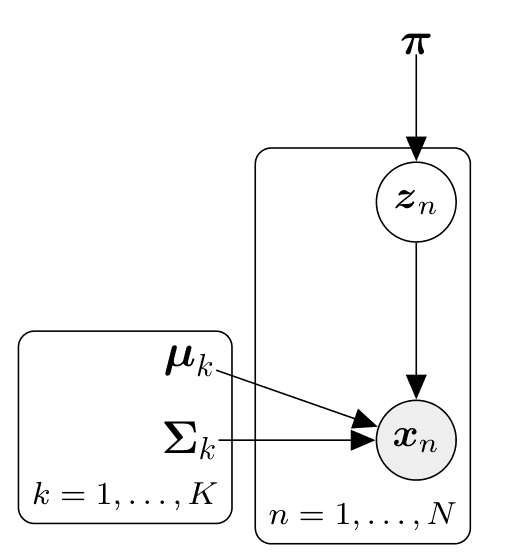
\includegraphics[width=320pt,keepaspectratio]{docs/images/Figure11.12.png}
\caption*{图 11.12}
\end{figure}


条件分布关于各个数据点分解为：

\begin{equation}
p(\boldsymbol{x}_1, \ldots, \boldsymbol{x}_N \mid \boldsymbol{z}_1, \ldots, \boldsymbol{z}_N) = \prod_{n=1}^N p(\boldsymbol{x}_n \mid \boldsymbol{z}_n) .
\tag{11.71}
\end{equation}

根据贝叶斯定理，后验概率分布自然扩展为：

\begin{equation}
p(z_{nk} = 1 \mid \boldsymbol{x}_n) = \frac{p(\boldsymbol{x}_n \mid z_{nk} = 1)p(z_{nk} = 1)}{\sum_{j=1}^K p(\boldsymbol{x}_n \mid z_{nj} = 1)p(z_{nj} = 1)} .
\tag{11.72a}
\end{equation}

\begin{equation}
\begin{adjustbox}{max width=\linewidth}
= \frac{\pi_k \mathcal{N}\left(\boldsymbol{x}_n \mid \boldsymbol{\mu}_k, \boldsymbol{\Sigma}_k\right)}{\sum_{j=1}^K \pi_j \mathcal{N}\left(\boldsymbol{x}_n \mid \boldsymbol{\mu}_j, \boldsymbol{\Sigma}_j\right)} = r_{nk} .
\end{adjustbox}
\tag{11.72b}
\end{equation}

这从第一性原理证明了：责任度 $ r_{nk} $ 精确等于在观测到数据点 $ \boldsymbol{x}_n $ 的条件下，其隐变量由第 $ k $ 个高斯分量生成的真实后验概率！

\medskip\hrule\medskip

\section*{11.4.5 重访 EM 算法}
\addcontentsline{toc}{subsection}{11.4.5 重访 EM 算法}

在隐变量视角下，EM 算法具有极为优美的理论解释。给定当前的参数设定 $ \boldsymbol{\theta}^{(t)} $：

\begin{itemize}
\item \textbf{E 步}：计算完整数据对数似然关于隐变量后验分布 $ p(\boldsymbol{z} \mid \boldsymbol{x}, \boldsymbol{\theta}^{(t)}) $ 的条件数学期望：
\end{itemize}

\begin{equation}
Q(\boldsymbol{\theta} \mid \boldsymbol{\theta}^{(t)}) = \mathbb{E}_{\boldsymbol{z} \mid \boldsymbol{x}, \boldsymbol{\theta}^{(t)}}\left[ \log p(\boldsymbol{x}, \boldsymbol{z} \mid \boldsymbol{\theta}) \right]
\tag{11.73a}
\end{equation}

\begin{equation}
= \sum_{\boldsymbol{z}} p(\boldsymbol{z} \mid \boldsymbol{x}, \boldsymbol{\theta}^{(t)}) \log p(\boldsymbol{x}, \boldsymbol{z} \mid \boldsymbol{\theta}) .
\tag{11.73b}
\end{equation}

\begin{itemize}
\item \textbf{M 步}：通过最大化该期望目标函数来选取更新后的模型参数：
\end{itemize}

\begin{equation}
\boldsymbol{\theta}^{(t+1)} = \arg\max_{\boldsymbol{\theta}} Q(\boldsymbol{\theta} \mid \boldsymbol{\theta}^{(t)}) .
\tag{11.74}
\end{equation}

通过展开 $ Q $ 函数并对其求导，能够以纯粹变分推断的严格范式无缝推导得出我们在 11.2 节求得的均值、协方差和混合权重的三大更新公式。

虽然 EM 迭代能确保对数似然单调不减，但它并不保证收敛到全局最大值，容易陷入次优的局部极大值点。在实际应用中，通常建议执行多次采用不同随机初始化的 EM 运行，以遴选具有最高最终对数似然的最优模型（Bishop, 2006; Rogers and Girolami, 2016）。

\section*{11.5 延伸阅读}
\addcontentsline{toc}{section}{11.5 延伸阅读}
\label{sec:11.5}

在本章中，我们重点讨论了用于概率密度估计的混合模型。在统计学与机器学习中，存在着极为丰富的密度估计技术体系。在实际工程与数据分析中，人们除了参数化混合模型外，还广泛使用非参数化的直方图与核密度估计方法。

\section*{直方图}
\addcontentsline{toc}{subsection}{直方图}

\emph{直方图（histogram）} 提供了表示连续概率密度的一种经典非参数方法，最早由 Pearson (1895) 提出。直方图的构建过程非常直观：将数据空间离散化划分为若干“区间箱”（bins），统计落入每个箱内的数据点数量；然后在每个区间的中心绘制一个矩形条，条柱的高度正比于该箱内的数据点频数。区间箱的宽度（bin size）是一个至关重要的超参数，选取过大容易导致欠拟合（过度平滑，抹杀局部细节），选取过小则极易导致过拟合（呈现杂乱的阶梯尖刺）。我们在 8.2.4 节讨论的交叉验证技术可用于在实践中自适应选择最优的箱宽。

\section*{核密度估计}
\addcontentsline{toc}{subsection}{核密度估计}

\emph{核密度估计（kernel density estimation, KDE）} 由 Rosenblatt (1956) 与 Parzen (1962) 独立提出，是一种基于样本点的非参数光滑密度估计技术。给定 $ N $ 个独立同分布样本点，核密度估计量将潜在的数据生成概率分布表示为：

\begin{equation}
p(x) = \frac{1}{Nh}\sum_{n=1}^N k\left( \frac{x - x_n}{h} \right)
\tag{11.75}
\end{equation}

其中 $ k(\cdot) $ 是一个核函数（即在实数域全域积分为 1 的非负光滑函数），$ h > 0 $ 是平滑带宽（bandwidth）超参数，其作用类似于直方图中的箱宽。

需要特别指出的是，与 GMM 将固定的 $ K $ 个高斯分量赋予可学习的均值和权重不同，核密度估计直接在数据集中的 \textbf{每一个具体样本点} $ x_n $ 处都放置一个固定形状的核基元函数。常用的核函数包括均匀分布核、Epanechnikov 核以及高斯核。核密度估计与直方图密切相关，但通过选用光滑可导的核函数（如高斯核），KDE 能够严格保证所得整体密度估计曲线的光滑性与连续可微性。


\begin{figure}[H]
\centering
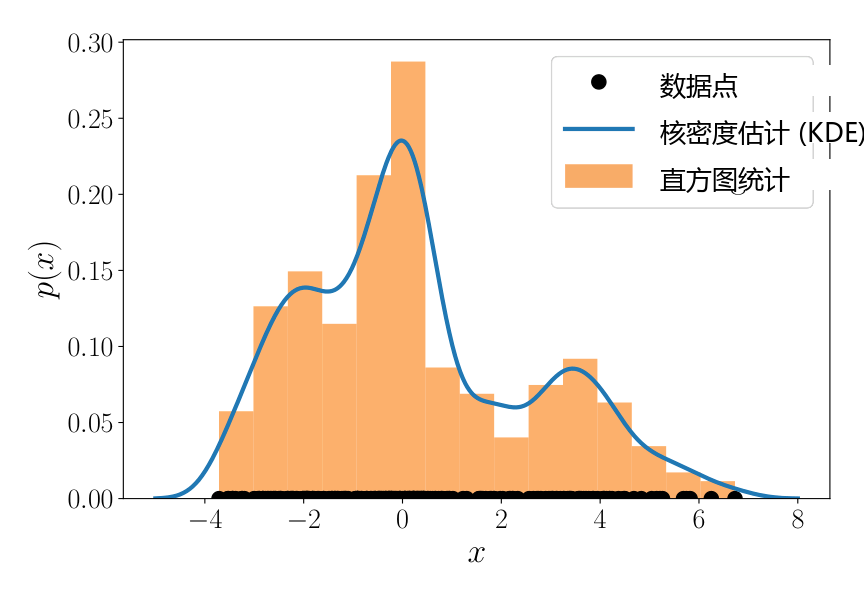
\includegraphics[width=0.92\textwidth,keepaspectratio]{docs/images/Figure11.13.png}
\caption*{图 11.13}
\end{figure}


图 11.13 直观对比了针对 250 个观测数据点，采用直方图与采用高斯核密度估计所得出的拟合分布。

\chapter{12 使用支持向量机分类}

在许多实际场景中，我们希望机器学习算法能够预测若干个（离散）结果之一。例如，电子邮件客户端将邮件分类为个人邮件和垃圾邮件，这对应着两种离散结果。另一个例子是天文望远镜识别夜空中的天体是星系、恒星还是行星。这类任务的结果数量通常较少，更重要的是，这些离散结果之间通常不存在额外的数学结构（例如大小顺序等；相比之下，T 恤的小号、中号和大号则是有序结构的离散结果）。在本章中，我们重点考虑输出为二元值的预测器，即只有两种可能结果的情形。这一机器学习任务被称为 \textbf{二元分类（binary classification）}。这与第 9 章讨论的连续值输出预测问题（回归）形成了鲜明对比。

在二元分类中，标签/输出能够取得的可能取值集合是二元的，在本章中我们统一用 $ \{+1, -1\} $ 来表示它们。换句话说，我们考虑如下形式的预测器：

\begin{equation}
f : \mathbb{R}^D \to \{+1, -1\} .
\tag{12.1}
\end{equation}

回顾第 8 章，我们将每个样本（数据点）$ \boldsymbol{x}_n $ 表示为一个由 $ D $ 个实数构成的特征向量。标签通常分别称为 \textbf{正类（positive class）} 和 \textbf{负类（negative class）}。读者应当注意，切勿主观地给 $ +1 $ 类赋予直觉上的“积极/褒义”属性。例如在癌症检测任务中，患有癌症的患者通常会被赋予 $ +1 $ 的标签。原则上，任何两个互异的值都可以用于表示类别，例如 $ \{\text{True}, \text{False}\} $、$ \{0, 1\} $ 或 $ \{\textcn{红}, \textcn{蓝}\} $。二元分类问题已经得到了广泛深入的研究，我们在 12.6 节中将对其他分类方法进行综述（对于概率模型而言，在数学上使用 $ \{0, 1\} $ 作为二元表示往往更为便利，参见例 6.12 后的说明）。

在本章中，我们将介绍一种用于解决二元分类任务的经典且强大的方法——\textbf{支持向量机（Support Vector Machine, SVM）}。与回归类似，分类同样属于监督学习任务：我们拥有一组样本 $ \boldsymbol{x}_n \in \mathbb{R}^D $ 及其对应的（二元）标签 $ y_n \in \{+1, -1\} $。给定一个由样本-标签对组成的训练数据集 $ \{(\boldsymbol{x}_1, y_1), \ldots, (\boldsymbol{x}_N, y_N)\} $，我们希望估计模型的参数，以获得最小的分类误差。类似于第 9 章，我们首先考虑线性模型，并通过对样本应用非线性特征变换 $ \boldsymbol{\phi} $（式 (9.13)）来处理非线性问题。我们将在 12.4 节深入重新审视特征变换 $ \boldsymbol{\phi} $ 与核方法。

支持向量机在众多应用领域中均能提供顶尖（state-of-the-art）的性能，并且具有坚实的统计学习理论保障（Steinwart and Christmann, 2008）。我们选择使用支持向量机来阐释二元分类主要基于以下两个重要原因：

\begin{enumerate}
\item \textbf{几何直观的机器学习视角}：SVM 为监督机器学习提供了一种非常优美而直观的几何思考方式。在第 9 章中，我们从概率模型的角度审视机器学习问题，并借助极大似然估计和贝叶斯推断来求解；而在本章中，我们将考虑一种替代路径——从几何角度推演机器学习任务。它高度依赖于我们在第 3 章中讨论的内积和正交投影等几何核心概念。
\item \textbf{带约束优化的综合实践}：与第 9 章不同，SVM 的优化目标函数不存在解析闭式解，因此我们必须借助第 7 章引入的拉格朗日乘子法、对偶理论等优化工具来进行求解。
\end{enumerate}


\begin{figure}[H]
\centering
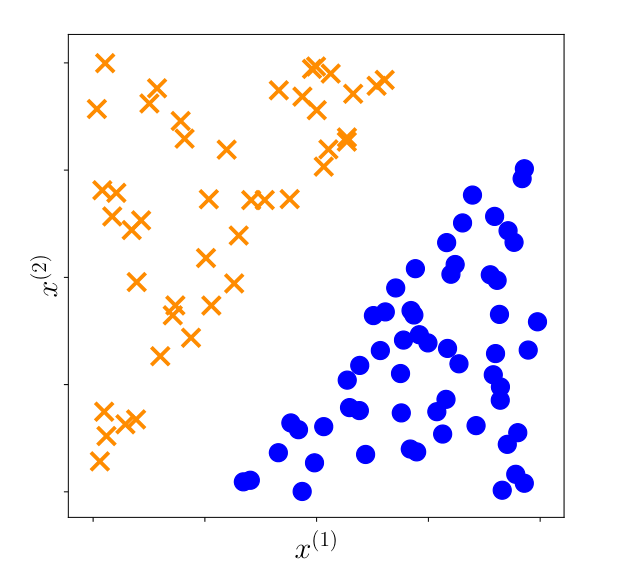
\includegraphics[width=0.92\textwidth,keepaspectratio]{docs/images/Figure12.1.png}
\caption*{图 12.1}
\end{figure}


支持向量机对待机器学习的视角与第 9 章的极大似然视角存在微妙而根本的差异。极大似然视角基于对数据分布的概率假设提出生成模型，并由此导出对应的优化目标；相比之下，SVM 视角则直接基于几何直观来构建训练时需要优化的特定目标函数。我们在第 10 章中已经见到过类似的思想——当时我们完全基于几何投影原则导出了主成分分析（PCA）。在 SVM 中，我们遵循经验风险最小化原则（8.2 节），直接设计一个在训练数据上最小化的目标函数，这也可以等价地理解为设计一种特殊的损失函数（合页损失）。

现在让我们来推导在样本-标签对上训练 SVM 所对应的优化问题。直观上，我们可以想象二元分类数据可以通过一个超平面进行完全分隔，如图 12.1 所示。在此图中，每个样本 $ \boldsymbol{x}_n $（二维向量）对应平面上的一个二维坐标点 $ (x_n^{(1)}, x_n^{(2)}) $，对应的二元标签 $ y_n $ 对应两种不同的标记符号（红色十字或蓝色实心圆）。“超平面（hyperplane）”是机器学习中的常用术语，我们在 2.8 节中已经详细讨论过。在 $ D $ 维向量空间中，超平面是维度为 $ D-1 $ 的仿射子空间。数据样本包含两个类别（有两种可能的标签），其特征（向量各分量）在空间中的几何分布允许我们通过绘制一条直线（二维平面中的超平面）将它们完全分开并正确分类。

在本章的后续部分：

\begin{itemize}
\item \textbf{12.1 节} 形式化两类数据的线性分隔超平面概念；
\item \textbf{12.2 节} 引入间隔（margin）的概念，推导原生支持向量机（Primal SVM），包括几何视角与损失函数视角，并拓展到允许分类错误的软间隔 SVM；
\item \textbf{12.3 节} 利用拉格朗日乘子法推导对偶支持向量机（Dual SVM），并展示其在样本凸包（convex hull）最近距离视角下的等价几何诠释；
\item \textbf{12.4 节} 介绍核方法（Kernels），展示如何将线性 SVM 推广为强大的非线性分类器；
\item \textbf{12.5 节} 讨论核化 SVM 凸二次规划问题的数值求解方法；
\item \textbf{12.6 节} 提供相关分类文献与理论拓展的延伸阅读。
\end{itemize}

\section*{12.1 分隔超平面}
\addcontentsline{toc}{section}{12.1 分隔超平面}
\label{sec:12.1}

给定表示为向量的两个样本 $ \boldsymbol{x}_i $ 和 $ \boldsymbol{x}_j $，计算它们之间相似度的一种经典方法是计算内积 $ \langle \boldsymbol{x}_i, \boldsymbol{x}_j \rangle $。回顾 3.2 节，内积与两个向量之间的夹角密切相关。两个向量之间的内积大小取决于各个向量的长度（范数）。此外，内积使我们能够严格定义正交性和投影等核心几何概念。

许多分类算法背后的核心思想，是将数据表示在空间 $ \mathbb{R}^D $ 中，然后对该空间进行划分——理想情况下，划分应使得具有相同标签的样本（且没有其他类别的样本）位于同一划分区域中。在二元分类的情形下，空间将被划分为分别对应于正类和负类的两个部分。我们考虑一种特别便利且基础的划分方式，即使用一个超平面将空间（线性地）切分为两半。设样本 $ \boldsymbol{x} \in \mathbb{R}^D $ 为数据空间中的一个元素。考虑由参数 $ \boldsymbol{w} \in \mathbb{R}^D $ 和标量截距 $ b \in \mathbb{R} $ 参数化的仿射函数：

\begin{equation}
f : \mathbb{R}^D \to \mathbb{R}
\tag{12.2a}
\end{equation}

\begin{equation}
\boldsymbol{x} \mapsto \langle \boldsymbol{w}, \boldsymbol{x} \rangle + b .
\tag{12.2b}
\end{equation}

回顾 2.8 节，超平面是仿射子空间。因此，在我们的二元分类问题中，我们将分隔两个类别的 \textbf{超平面（hyperplane）} 定义为函数 $ f(\boldsymbol{x}) = 0 $ 的水平集：

\begin{equation}
\{ \boldsymbol{x} \in \mathbb{R}^D : f(\boldsymbol{x}) = 0 \} .
\tag{12.3}
\end{equation}


\begin{figure}[H]
\centering
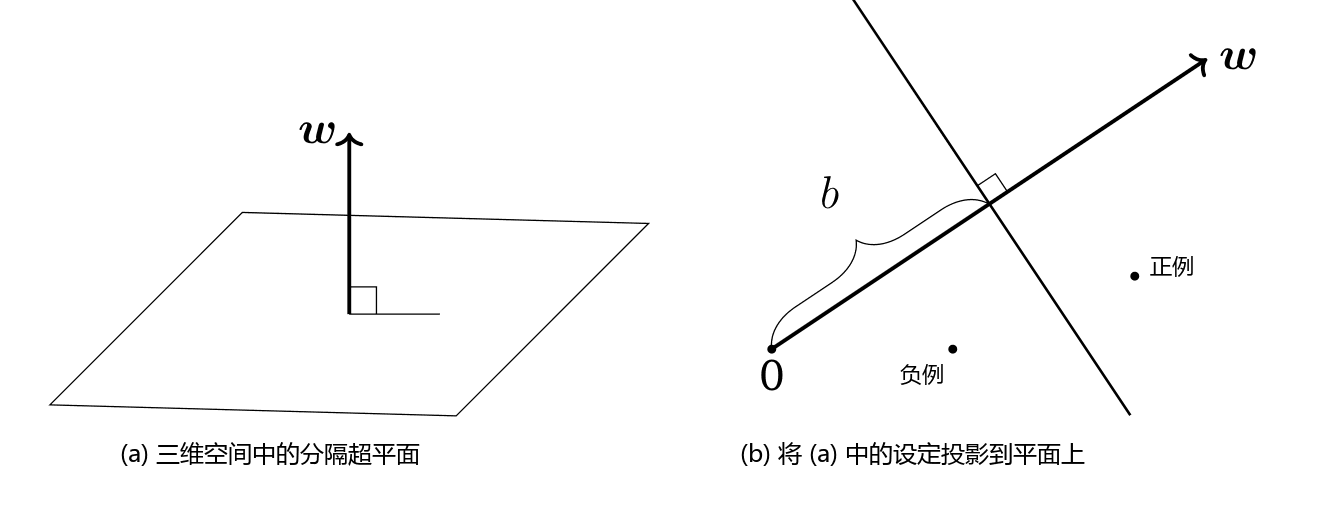
\includegraphics[width=0.92\textwidth,keepaspectratio]{docs/images/Figure12.2.png}
\caption*{图 12.2}
\end{figure}


图 12.2 给出了该超平面的几何示意图，其中向量 $ \boldsymbol{w} $ 是超平面的法向量（normal vector），$ b $ 是截距（intercept）。我们可以通过在超平面上任取两个样本点 $ \boldsymbol{x}_a $ 和 $ \boldsymbol{x}_b $，并证明它们之间的差值向量与 $ \boldsymbol{w} $ 正交，从而严格推导出 $ \boldsymbol{w} $ 确实是超平面 (12.3) 的法向量。以等式形式写出：

\begin{equation}
f(\boldsymbol{x}_a) - f(\boldsymbol{x}_b) = \langle \boldsymbol{w}, \boldsymbol{x}_a \rangle + b - (\langle \boldsymbol{w}, \boldsymbol{x}_b \rangle + b)
\tag{12.4a}
\end{equation}

\begin{equation}
= \langle \boldsymbol{w}, \boldsymbol{x}_a - \boldsymbol{x}_b \rangle
\tag{12.4b}
\end{equation}

其中第二行是由内积的双线性（3.2 节）直接得到的。由于我们选择的 $ \boldsymbol{x}_a $ 和 $ \boldsymbol{x}_b $ 都位于超平面上，根据定义必然有 $ f(\boldsymbol{x}_a) = 0 $ 且 $ f(\boldsymbol{x}_b) = 0 $，由此可得：

\begin{equation*}
\langle \boldsymbol{w}, \boldsymbol{x}_a - \boldsymbol{x}_b \rangle = 0 .
\end{equation*}

回顾可知，当两个向量的内积为零时，它们相互正交。因此，我们严格证明了向量 $ \boldsymbol{w} $ 与超平面上的任意位移向量均正交，即 $ \boldsymbol{w} $ 是超平面的法向量。

\medskip\hrule\medskip

\textbf{说明（关于向量的双重理解）} 回顾第 2 章，我们指出在不同情境下可以以不同的方式理解“向量”。在本章中：

\begin{itemize}
\item 我们将参数向量 $ \boldsymbol{w} $ 视作一个指示几何方向的箭头，即将其视为\textbf{几何向量}；
\item 相比之下，我们将样本向量 $ \boldsymbol{x} $ 视作数据点（由其坐标值确定），即将其视为标准基下的\textbf{坐标向量}。  
\end{itemize}

♦

\medskip\hrule\medskip

当给定一个新的测试样本 $ \boldsymbol{x}_{\text{test}} $ 时，我们根据该样本落在超平面的哪一侧将其分类为正类或负类。需要特别注意的是，方程 (12.3) 不仅定义了一个超平面，还附带定义了一个朝向——也就是说，它明确划分了超平面的正侧（positive side）与负侧（negative side）。因此，为了对测试样本 $ \boldsymbol{x}_{\text{test}} $ 进行分类，我们只需计算函数值 $ f(\boldsymbol{x}_{\text{test}}) $，并在满足以下规则时进行判定：

\begin{equation*}
\hat{y} = \begin{cases} +1, & \textcn{若 } f(\boldsymbol{x}_{\text{test}}) \geqslant 0 \\ -1, & \textcn{若 } f(\boldsymbol{x}_{\text{test}}) < 0 \end{cases} .
\end{equation*}

从几何直观上讲，正样本位于超平面的“上方”，而负样本位于超平面的“下方”。

在训练分类器时，我们希望确保带有正标签的样本都落在超平面的正侧，即：

\begin{equation}
\langle \boldsymbol{w}, \boldsymbol{x}_n \rangle + b \geqslant 0 \quad \textcn{当 } y_n = +1 \textcn{时}
\tag{12.5}
\end{equation}

同时确保带有负标签的样本都落在超平面的负侧，即：

\begin{equation}
\langle \boldsymbol{w}, \boldsymbol{x}_n \rangle + b < 0 \quad \textcn{当 } y_n = -1 \textcn{时} .
\tag{12.6}
\end{equation}

读者可参考图 12.2(b) 获得正负样本几何分布的直观感受。在数学上，这两个条件通常可以合并为一个极为紧凑的唯一样本判别约束不等式：

\begin{equation}
y_n (\langle \boldsymbol{w}, \boldsymbol{x}_n \rangle + b) \geqslant 0 .
\tag{12.7}
\end{equation}

当我们将式 (12.5) 和式 (12.6) 的两端分别乘以对应的标签取值 $ y_n = 1 $ 和 $ y_n = -1 $ 时，即可立即验证式 (12.7) 与式 (12.5) 及 (12.6) 是完全等价的。

\section*{12.2 原生支持向量机}
\addcontentsline{toc}{section}{12.2 原生支持向量机}
\label{sec:12.2}

基于点到超平面的距离概念，我们现在可以正式讨论支持向量机（Support Vector Machine, SVM）。对于一个线性可分的数据集 $ \{(\boldsymbol{x}_1, y_1), \ldots, (\boldsymbol{x}_N, y_N)\} $，存在无穷多个候选分隔超平面（参见图 12.3），从而对应着无穷多个能够在训练集上实现零误差分类的线性分类器。


\begin{figure}[H]
\centering
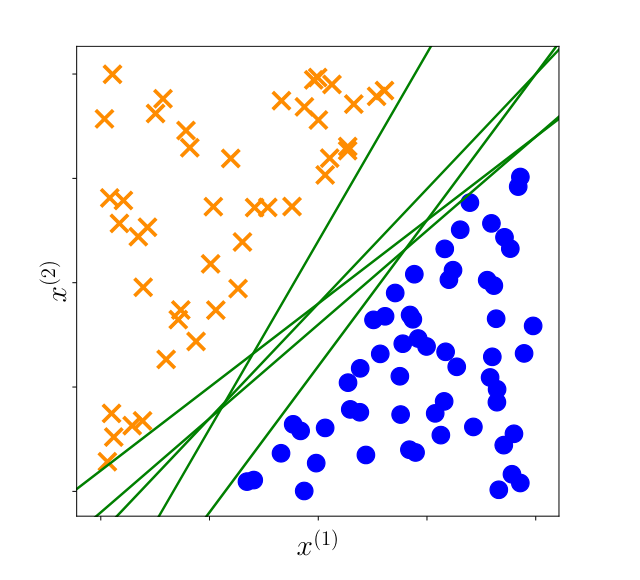
\includegraphics[width=0.92\textwidth,keepaspectratio]{docs/images/Figure12.3.png}
\caption*{图 12.3}
\end{figure}


为了找到唯一确定的最优解，一个核心思想是选择能够使正负样本之间 \textbf{间隔（margin）} 最大化的分隔超平面。换句话说，我们希望正例和负例被一个尽可能大的间隔所分隔开（12.2.1 节）。理论表明，具有较大间隔的分类器往往具有极佳的泛化性能（Steinwart and Christmann, 2008）。在接下来的内容中，我们通过计算样本点到超平面的距离来正式推导间隔。回顾 3.8 节，给定一个样本点 $ \boldsymbol{x}_n $，超平面上距离该点最近的点可以通过 \textbf{正交投影（orthogonal projection）} 获得。

\medskip\hrule\medskip

\section*{12.2.1 间隔的概念}
\addcontentsline{toc}{subsection}{12.2.1 间隔的概念}

“间隔”的概念在直观上十分简单：假设数据集是线性可分的，那么间隔就是分隔超平面到数据集中 \textbf{距离其最近的样本点} 的垂直几何距离（到超平面距离最近的样本点可能有两个或更多）。然而，在尝试严格形式化这一距离时，会出现一个容易引起混淆的技术细节——我们必须明确度量该距离的 \textbf{尺度（scale）}。

一个潜在的尺度是直接考虑数据本身的尺度，即 $ \boldsymbol{x}_n $ 的原始数值大小。但这种做法存在严重问题：如果我们改变 $ \boldsymbol{x}_n $ 的度量单位（例如从米转换为毫米），$ \boldsymbol{x}_n $ 中的数值就会改变，从而导致计算出的距离数值发生改变。正如我们稍后所见，我们依据超平面方程 (12.3) 本身来定义度量尺度。


\begin{figure}[H]
\centering
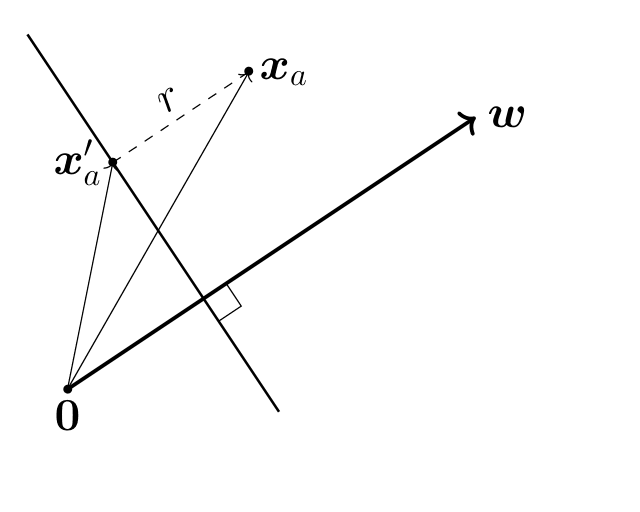
\includegraphics[width=0.92\textwidth,keepaspectratio]{docs/images/Figure12.4.png}
\caption*{图 12.4}
\end{figure}


考虑超平面 $ \langle \boldsymbol{w}, \boldsymbol{x} \rangle + b = 0 $ 和一个样本点 $ \boldsymbol{x}_a $，如图 12.4 所示。不失一般性，我们可以假设样本 $ \boldsymbol{x}_a $ 位于超平面的正侧，即 $ \langle \boldsymbol{w}, \boldsymbol{x}_a \rangle + b > 0 $。我们希望计算 $ \boldsymbol{x}_a $ 到超平面的垂直几何距离 $ r > 0 $。为此，我们考虑 $ \boldsymbol{x}_a $ 在超平面上的正交投影（3.8 节），记作 $ \boldsymbol{x}'_a $。

由于法向量 $ \boldsymbol{w} $ 与超平面正交，我们知道从 $ \boldsymbol{x}'_a $ 到 $ \boldsymbol{x}_a $ 的位移向量正好沿着 $ \boldsymbol{w} $ 的方向，因此该位移就是向量 $ \boldsymbol{w} $ 的某种缩放。为了方便，我们选择使用长度为 1 的单位法向量 $ \frac{\boldsymbol{w}}{\|\boldsymbol{w}\|} $。利用向量加法（2.4 节），我们可以将 $ \boldsymbol{x}_a $ 严格表示为：

\begin{equation}
\boldsymbol{x}_a = \boldsymbol{x}'_a + r \frac{\boldsymbol{w}}{\|\boldsymbol{w}\|} .
\tag{12.8}
\end{equation}

理解标量距离 $ r $ 的另一种方式是：它是向量 $ \boldsymbol{x}_a - \boldsymbol{x}'_a $ 在由单位向量 $ \frac{\boldsymbol{w}}{\|\boldsymbol{w}\|} $ 张成的一维子空间中的坐标。此时，我们已将 $ \boldsymbol{x}_a $ 到超平面的距离精确表示为 $ r $。如果我们将 $ \boldsymbol{x}_a $ 取为整个数据集中距离超平面最近的样本点，那么该距离 $ r $ 即为分类器的 \textbf{间隔（margin）}。

回顾前文，我们希望所有正样本到超平面的距离都大于等于 $ r $，且所有负样本（在负方向上）到超平面的距离也至少为 $ r $。类似于将式 (12.5) 与 (12.6) 合并为式 (12.7)，我们可以将这一几何要求统一表述为：

\begin{equation}
y_n (\langle \boldsymbol{w}, \boldsymbol{x}_n \rangle + b) \geqslant r .
\tag{12.9}
\end{equation}

换句话说，我们将“所有正负样本距离超平面至少为 $ r $”的要求合并成了一个单一的不等式。

由于此时超平面的朝向仅由 $ \boldsymbol{w} $ 的方向决定，我们在模型中引入假设：参数向量 $ \boldsymbol{w} $ 的长度被归一化为单位长度，即 $ \|\boldsymbol{w}\| = 1 $（这里采用欧几里得范数 $ \|\boldsymbol{w}\| = \sqrt{\boldsymbol{w}^\top \boldsymbol{w}} $，3.1 节）。这一归一化假设使得距离 $ r $ 在式 (12.8) 中具有极其直观的几何意义——它就是单位长度向量的实际缩放系数。

\medskip\hrule\medskip

\textbf{说明（关于间隔的不同形式化表述）} 熟悉支持向量机其他教材阐述的读者可能会注意到，我们在此处引入的 $ \|\boldsymbol{w}\| = 1 $ 约束不同于标准的经典表述（例如 Schölkopf and Smola, 2002 中直接固定函数间隔为 1 的推导）。在 12.2.3 节中，我们将严格证明这两种表述途径是完全等价的。 ♦

\medskip\hrule\medskip

将上述要求综合为一个带约束的优化问题，我们得到：

\begin{equation}
\max_{\boldsymbol{w}, b, r} \underbrace{r}_{\textcn{间隔}}
\tag{12.10}
\end{equation}

\begin{equation*}
\text{subject to } \underbrace{y_n (\langle \boldsymbol{w}, \boldsymbol{x}_n \rangle + b) \geqslant r}_{\textcn{数据拟合约束}} , \quad \underbrace{\|\boldsymbol{w}\| = 1}_{\textcn{法向量归一化}} , \quad r > 0
\end{equation*}

式 (12.10) 的含义非常纯粹：我们希望在保证所有数据点都位于超平面正确一侧的前提下，使几何间隔 $ r $ 最大化。

\medskip\hrule\medskip

\textbf{说明（间隔在机器学习理论中的深远意义）} “间隔”的概念在统计机器学习中具有基础性的广泛意义。Vladimir Vapnik 和 Alexey Chervonenkis 正是通过利用间隔证明了：当分类间隔较大时，分类函数族的“容量（capacity）/复杂度”较低，从而保证了学习的泛化能力（Vapnik, 2000）。事实证明，这一概念在现代统计学习理论中分析泛化误差边界时不可或缺（Steinwart and Christmann, 2008; Shalev-Shwartz and Ben-David, 2014）。 ♦

\medskip\hrule\medskip

\section*{12.2.2 间隔的传统推导}
\addcontentsline{toc}{subsection}{12.2.2 间隔的传统推导}

在上一小节中，我们基于“仅关心 $ \boldsymbol{w} $ 的方向而非其长度”的观察推导出了式 (12.10)，从而引入了 $ \|\boldsymbol{w}\| = 1 $ 的假设。在本小节中，我们通过引入另一种不同的视角来推导间隔最大化问题。

我们不再约束参数向量的长度归一化，而是选择对\textbf{数据预测输出的尺度}进行规范。具体而言，我们设定度量尺度，使得预测器 $ \langle \boldsymbol{w}, \boldsymbol{x} \rangle + b $ 在距离超平面最近的样本点处的取值恰好为 $ 1 $。设数据集中距离超平面最近的样本点为 $ \boldsymbol{x}_a $（当前仍假定数据线性可分）。


\begin{figure}[H]
\centering
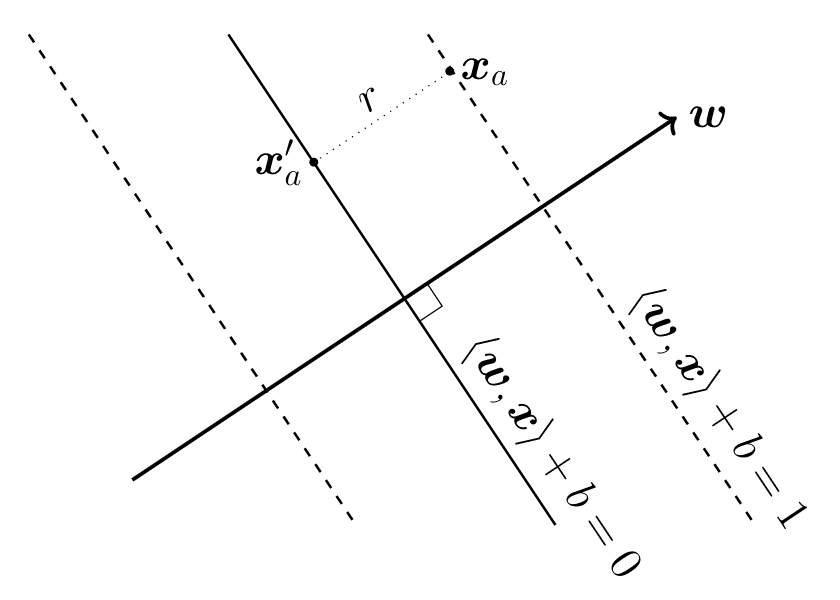
\includegraphics[width=0.92\textwidth,keepaspectratio]{docs/images/Figure12.5.png}
\caption*{图 12.5}
\end{figure}


图 12.5 与图 12.4 在几何结构上完全相同，唯一的区别在于我们重新对预测输出的尺度进行了缩放，使得样本 $ \boldsymbol{x}_a $ 恰好落在正间隔边界超平面上，即：

\begin{equation*}
\langle \boldsymbol{w}, \boldsymbol{x}_a \rangle + b = 1 .
\end{equation*}

由于 $ \boldsymbol{x}'_a $ 是 $ \boldsymbol{x}_a $ 在超平面上的正交投影，根据定义它必然严格落在超平面上，即：

\begin{equation}
\langle \boldsymbol{w}, \boldsymbol{x}'_a \rangle + b = 0 .
\tag{12.11}
\end{equation}

将式 (12.8) 的几何向量分解式 $ \boldsymbol{x}'_a = \boldsymbol{x}_a - r \frac{\boldsymbol{w}}{\|\boldsymbol{w}\|} $ 代入式 (12.11)，我们得到：

\begin{equation}
\left\langle \boldsymbol{w}, \boldsymbol{x}_a - r \frac{\boldsymbol{w}}{\|\boldsymbol{w}\|} \right\rangle + b = 0 .
\tag{12.12}
\end{equation}

利用内积的双线性性质（3.2 节），展开上式：

\begin{equation}
\langle \boldsymbol{w}, \boldsymbol{x}_a \rangle + b - r \frac{\langle \boldsymbol{w}, \boldsymbol{w} \rangle}{\|\boldsymbol{w}\|} = 0 .
\tag{12.13}
\end{equation}

注意到前两项根据我们对尺度的设定恰好等于 $ 1 $，即 $ \langle \boldsymbol{w}, \boldsymbol{x}_a \rangle + b = 1 $。又根据式 (3.16)，内积 $ \langle \boldsymbol{w}, \boldsymbol{w} \rangle = \|\boldsymbol{w}\|^2 $。因此第三项化简为：

\begin{equation*}
r \frac{\|\boldsymbol{w}\|^2}{\|\boldsymbol{w}\|} = r \|\boldsymbol{w}\| .
\end{equation*}

代入式 (12.13) 即得：

\begin{equation}
1 - r \|\boldsymbol{w}\| = 0 \implies r = \frac{1}{\|\boldsymbol{w}\|} .
\tag{12.14}
\end{equation}

这是一个极为优美且关键的结论：\textbf{几何间隔 $ r $ 恰好等于超平面法向量模长的倒数 $ \frac{1}{\|\boldsymbol{w}\|} $}！

初看起来，这个等式可能略显反直觉：我们似乎用一个尚未确定的向量 $ \boldsymbol{w} $ 的模长来表达了几何距离 $ r $。理解这一点的一种有效视角是将距离 $ r $ 视为推导过程中的一个辅助变量。因此，在本节的后续讨论中，我们统一使用 $ \frac{1}{\|\boldsymbol{w}\|} $ 来表示到超平面的几何距离。在 12.2.3 节中，我们将严格证明选择间隔为 $ 1 $ 与 12.2.1 节中假设 $ \|\boldsymbol{w}\| = 1 $ 在数学上完全等价。

类似于得出式 (12.9) 的推导，我们要求所有的正负样本点到超平面的函数间隔至少为 $ 1 $：

\begin{equation}
y_n (\langle \boldsymbol{w}, \boldsymbol{x}_n \rangle + b) \geqslant 1 .
\tag{12.15}
\end{equation}

将最大化间隔 $ r = \frac{1}{\|\boldsymbol{w}\|} $ 与分类正确性约束相结合，我们得到优化问题：

\begin{equation}
\max_{\boldsymbol{w}, b} \frac{1}{\|\boldsymbol{w}\|}
\tag{12.16}
\end{equation}

\begin{equation}
\text{subject to } y_n (\langle \boldsymbol{w}, \boldsymbol{x}_n \rangle + b) \geqslant 1, \quad \forall n = 1, \ldots, N .
\tag{12.17}
\end{equation}

在优化理论与实际计算中，相比于直接最大化范数的倒数，最大化 $ \frac{1}{\|\boldsymbol{w}\|} $ 等价于最小化范数 $ \|\boldsymbol{w}\| $，进而等价于最小化范数的平方 $ \frac{1}{2}\|\boldsymbol{w}\|^2 $（引入系数 $ \frac{1}{2} $ 不改变最优点位置，但可以在求导时消去平方项产生的系数 2，带来更整洁的梯度形式）。于是，优化目标转化为标准的凸二次规划形式：

\begin{equation}
\min_{\boldsymbol{w}, b} \frac{1}{2} \|\boldsymbol{w}\|^2
\tag{12.18}
\end{equation}

\begin{equation}
\text{subject to } y_n (\langle \boldsymbol{w}, \boldsymbol{x}_n \rangle + b) \geqslant 1, \quad \forall n = 1, \ldots, N .
\tag{12.19}
\end{equation}

式 (12.18) 被称为 \textbf{硬间隔支持向量机（Hard Margin SVM）}。之所以称为“硬（hard）”，是因为该公式具有严格的约束，不允许任何样本点侵入间隔边界内部或落在错误的一侧。在 12.2.4 节中，我们将放宽这一硬性约束，以优雅地应对非线性可分的数据集。

\medskip\hrule\medskip

\section*{12.2.3 为什么可以将间隔设为 1}
\addcontentsline{toc}{subsection}{12.2.3 为什么可以将间隔设为 1}

在 12.2.1 节中，我们旨在最大化表示最近样本点到超平面几何距离的变量 $ r $；而在 12.2.2 节中，我们直接对数据尺度进行了缩放，使得最近样本点处的预测值为 1。在本小节中，我们通过一个严格的数学定理说明这两种推导完全等价。

\medskip\hrule\medskip

\textbf{定理 12.1} 在权重归一化假定下最大化几何间隔 $ r $ 的优化问题 (12.10)：

\begin{equation}
\max_{\boldsymbol{w}, b, r} \underbrace{r}_{\textcn{间隔}} \quad \text{subject to } y_n (\langle \boldsymbol{w}, \boldsymbol{x}_n \rangle + b) \geqslant r, \quad \|\boldsymbol{w}\| = 1, \quad r > 0
\tag{12.20}
\end{equation}

与将最近样本处的函数间隔固定为 1 后的优化问题：

\begin{equation}
\min_{\boldsymbol{w}, b} \underbrace{\frac{1}{2} \|\boldsymbol{w}\|^2}_{\textcn{间隔项}} \quad \text{subject to } \underbrace{y_n (\langle \boldsymbol{w}, \boldsymbol{x}_n \rangle + b) \geqslant 1}_{\textcn{数据拟合约束}}
\tag{12.21}
\end{equation}

在几何上是完全等价的。

\medskip\hrule\medskip

\textbf{证明} 考虑优化问题 (12.20)。由于平方变换在非负实数区间上是严格单调递增的，因此将目标函数替换为 $ r^2 $ 不会改变最优解。由于 $ \|\boldsymbol{w}\| = 1 $，我们可以引入一个未归一化的新权重向量 $ \boldsymbol{w}' $，并通过显式使用单位向量 $ \frac{\boldsymbol{w}'}{\|\boldsymbol{w}'\|} $ 来重新参数化目标：

\begin{equation}
\max_{\boldsymbol{w}', b, r} r^2 \quad \text{subject to } y_n \left( \left\langle \frac{\boldsymbol{w}'}{\|\boldsymbol{w}'\|}, \boldsymbol{x}_n \right\rangle + b \right) \geqslant r, \quad r > 0 .
\tag{12.22}
\end{equation}

由于式 (12.22) 显式声明了几何距离 $ r > 0 $（由线性可分假设保证），我们可以将第一个约束不等式的两端同时除以 $ r $：

\begin{equation}
\begin{adjustbox}{max width=\linewidth}
\max_{\boldsymbol{w}', b, r} r^2 \quad \text{subject to } y_n \left( \left\langle \underbrace{\frac{\boldsymbol{w}'}{\|\boldsymbol{w}'\| r}}_{\boldsymbol{w}''}, \boldsymbol{x}_n \right\rangle + \underbrace{\frac{b}{r}}_{b''} \right) \geqslant 1, \quad r > 0 .
\end{adjustbox}
\tag{12.23}
\end{equation}

定义新参数 $ \boldsymbol{w}'' = \frac{\boldsymbol{w}'}{\|\boldsymbol{w}'\| r} $ 和 $ b'' = \frac{b}{r} $。对 $ \boldsymbol{w}'' $ 两端取范数：

\begin{equation}
\begin{adjustbox}{max width=\linewidth}
\|\boldsymbol{w}''\| = \left\| \frac{\boldsymbol{w}'}{\|\boldsymbol{w}'\| r} \right\| = \frac{1}{r} \left\| \frac{\boldsymbol{w}'}{\|\boldsymbol{w}'\|} \right\| = \frac{1}{r} \implies r = \frac{1}{\|\boldsymbol{w}''\|} .
\end{adjustbox}
\tag{12.24}
\end{equation}

将 $ r^2 = \frac{1}{\|\boldsymbol{w}''\|^2} $ 代入式 (12.23) 的目标函数中，优化问题重写为：

\begin{equation}
\max_{\boldsymbol{w}'', b''} \frac{1}{\|\boldsymbol{w}''\|^2} \quad \text{subject to } y_n (\langle \boldsymbol{w}'', \boldsymbol{x}_n \rangle + b'') \geqslant 1 .
\tag{12.25}
\end{equation}

最后一步注意到，最大化 $ \frac{1}{\|\boldsymbol{w}''\|^2} $ 与最小化 $ \frac{1}{2} \|\boldsymbol{w}''\|^2 $ 具有完全相同的最优解。由此定理 12.1 得证。 $ \blacksquare $

\medskip\hrule\medskip

\section*{12.2.4 软间隔 SVM：几何视角}
\addcontentsline{toc}{subsection}{12.2.4 软间隔 SVM：几何视角}

在实际应用中，数据通常不是线性可分的。此时，我们必须允许某些样本点落入间隔区域内部，甚至落在超平面的错误一侧，如图 12.6 所示。


\begin{figure}[H]
\centering
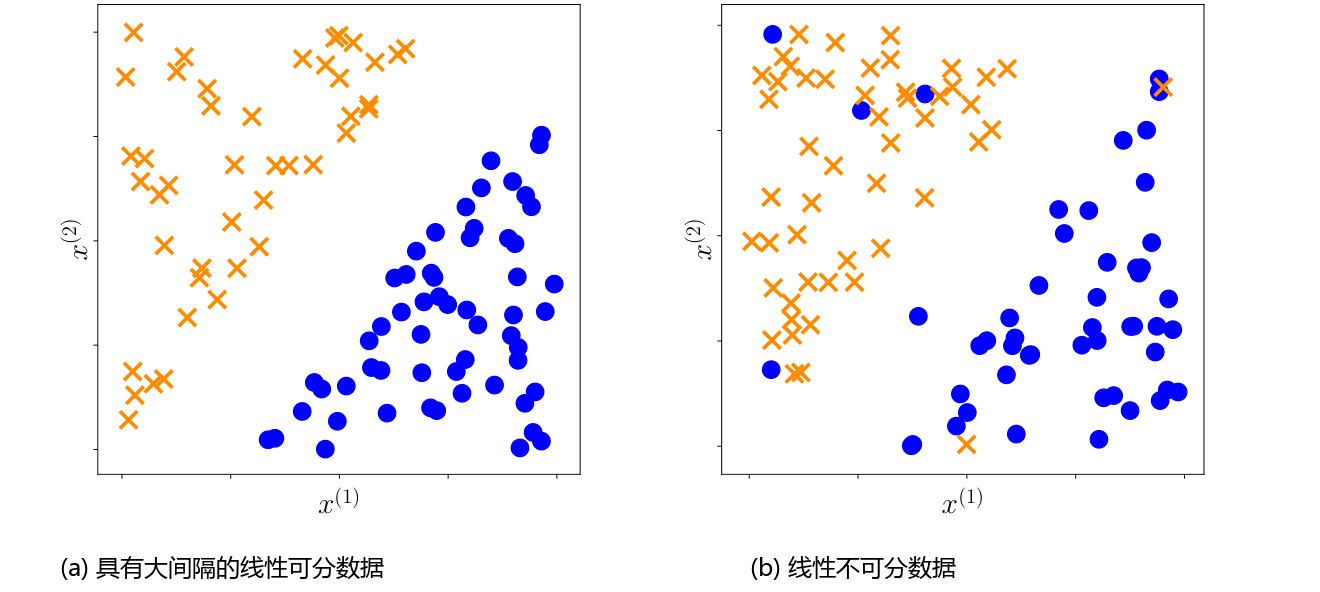
\includegraphics[width=0.92\textwidth,keepaspectratio]{docs/images/Figure12.6.png}
\caption*{图 12.6}
\end{figure}


允许一定分类错误的模型被称为 \textbf{软间隔支持向量机（Soft Margin SVM）}。在本节中，我们首先使用直观的几何推导来导出其优化问题；在 12.2.5 节中，我们将利用损失函数的思想导出等价的目标；在 12.3 节中，我们将借助拉格朗日乘子法导出对偶优化问题，并由此揭示软间隔 SVM 的第三种等价诠释——基于样本凸包最近距离的几何对偶图景（12.3.2 节）。

解决线性不可分问题的关键几何构想，是为每个样本-标签对 $ (\boldsymbol{x}_n, y_n) $ 引入一个 \textbf{松弛变量（slack variable）} $ \xi_n \geqslant 0 $。松弛变量允许特定样本侵入间隔区域甚至越过分隔超平面（参见图 12.7）。


\begin{figure}[H]
\centering
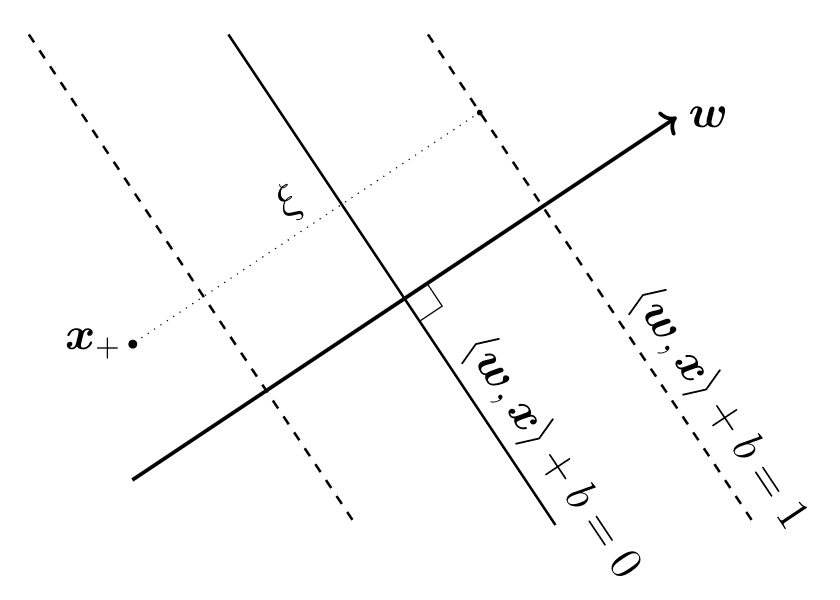
\includegraphics[width=0.92\textwidth,keepaspectratio]{docs/images/Figure12.7.png}
\caption*{图 12.7}
\end{figure}


如图 12.7 所示，对于正样本 $ \boldsymbol{x}_+ $，当其未能达到正边界 $ \langle \boldsymbol{w}, \boldsymbol{x}_+ \rangle + b = 1 $ 时，其到该边界的垂直偏移量即为 $ \xi_+ $。因此，我们从间隔边界中减去松弛量 $ \xi_n $，同时约束 $ \xi_n \geqslant 0 $。为了促使分类器尽可能正确分类更多样本，我们在最小化目标中对所有松弛变量之和进行惩罚：

\begin{equation}
\min_{\boldsymbol{w}, b, \boldsymbol{\xi}} \frac{1}{2} \|\boldsymbol{w}\|^2 + C \sum_{n=1}^N \xi_n
\tag{12.26a}
\end{equation}

\begin{equation}
\text{subject to } y_n (\langle \boldsymbol{w}, \boldsymbol{x}_n \rangle + b) \geqslant 1 - \xi_n
\tag{12.26b}
\end{equation}

\begin{equation}
\xi_n \geqslant 0 , \quad \forall n = 1, \ldots, N .
\tag{12.26c}
\end{equation}

与硬间隔 SVM (12.18) 相比，这一带有松弛变量的问题正是著名的 \textbf{软间隔 SVM}（因其参数形式通常亦称为 \textbf{$ C $-SVM}）。

超参数 $ C > 0 $ 在 \textbf{最大化间隔} 与 \textbf{最小化总松弛违背量} 之间进行权衡。该参数被称为 \textbf{正则化参数（regularization parameter）}：

\begin{itemize}
\item 当 $ C $ 很大时，意味着对松弛违背的惩罚极重，分类器将极力避免任何样本侵入间隔，逼近硬间隔 SVM；
\item 当 $ C $ 较小时，分类器更看重间隔项 $ \frac{1}{2}\|\boldsymbol{w}\|^2 $ 的最小化，从而容忍更多样本落入间隔或被轻微误分，以此换取更大的几何间隔和更好的泛化抗噪能力。
\end{itemize}

\medskip\hrule\medskip

\textbf{说明（未受正则化的截距 $ b $）} 在软间隔 SVM (12.26a) 的公式表述中，权重向量 $ \boldsymbol{w} $ 受到了范数惩罚（即被正则化），但截距项 $ b $ \textbf{未受正则化}（目标函数中不包含 $ b^2 $ 项）。未正则化的截距项 $ b $ 在理论分析上引入了额外的复杂性（Steinwart and Christmann, 2008, 第 1 章），并且会在一定程度上增加数值求解的算法开销（Fan et al., 2008）。 ♦

\medskip\hrule\medskip

\section*{12.2.5 软间隔 SVM：损失函数视角}
\addcontentsline{toc}{subsection}{12.2.5 软间隔 SVM：损失函数视角}

现在让我们遵循经验风险最小化原则（8.2 节），从一个截然不同但完全等价的视角——损失函数的角度重新审视 SVM。

在支持向量机中，我们选择超平面作为假设类（hypothesis class）：

\begin{equation}
f(\boldsymbol{x}) = \langle \boldsymbol{w}, \boldsymbol{x} \rangle + b .
\tag{12.27}
\end{equation}

我们将会看到，几何间隔最大化直接对应于目标函数中的正则化项。接下来的核心问题是：\textbf{对应的损失函数究竟是什么？}

与第 9 章讨论的连续值回归问题不同，二元分类的输出标签属于离散集合 $ \{+1, -1\} $。因此，用于衡量预测偏差的损失函数必须专门适配二元分类任务。例如，回归中广泛使用的平方损失（式 (9.10b)）并不适合二元分类。

\medskip\hrule\medskip

\textbf{说明（0-1 损失与组合优化的困境）} 在二元分类中，最符合直觉的理想损失函数是直接统计预测标签与真实标签之间的不匹配次数：如果预测类别与真实标签一致，损失为 0；如果两者不一致，损失为 1。这一损失函数记作 $ \mathbf{1}(f(\boldsymbol{x}_n) \neq y_n) $，称为 \textbf{0-1 损失（zero-one loss）}。 不幸的是，0-1 损失是非连续、非凸且阶跃跳变的，直接最小化 0-1 损失将导出一个极其困难的 \textbf{组合优化问题（combinatorial optimization problem）}，这在计算复杂度上属于 NP-难问题。 ♦

\medskip\hrule\medskip

支持向量机所对应的凸替代损失函数是什么？考虑预测器输出 $ f(\boldsymbol{x}_n) $ 与真实标签 $ y_n $ 之间的乘积。导出软间隔 SVM (12.26a) 的等价途径是引入著名的 \textbf{合页损失（hinge loss）}：

\begin{equation}
\ell(t) = \max\{0, 1 - t\} , \quad \textcn{其中 } t = y f(\boldsymbol{x}) = y (\langle \boldsymbol{w}, \boldsymbol{x} \rangle + b) .
\tag{12.28}
\end{equation}

让我们考察合页损失在不同预测状态下的取值规律：

\begin{enumerate}
\item 若样本被正确分类且距离超平面大于等于 1（即 $ t \geqslant 1 $），样本落在正规间隔之外，合页损失为 $ 0 $；
\item 若样本被正确分类但距离超平面过近（即 $ 0 < t < 1 $），样本侵入了间隔区域内部，此时虽然预测方向正确，但仍会承受 $ 1 - t > 0 $ 的线性惩罚；
\item 若样本落在超平面的错误一侧（即 $ t \leqslant 0 $），样本被错误分类，此时合页损失将承受更大的线性增长惩罚。
\end{enumerate}

换言之，\textbf{一旦样本距离超平面的距离小于间隔，即使分类正确，我们也要对其施加线性惩罚}！


\begin{figure}[H]
\centering
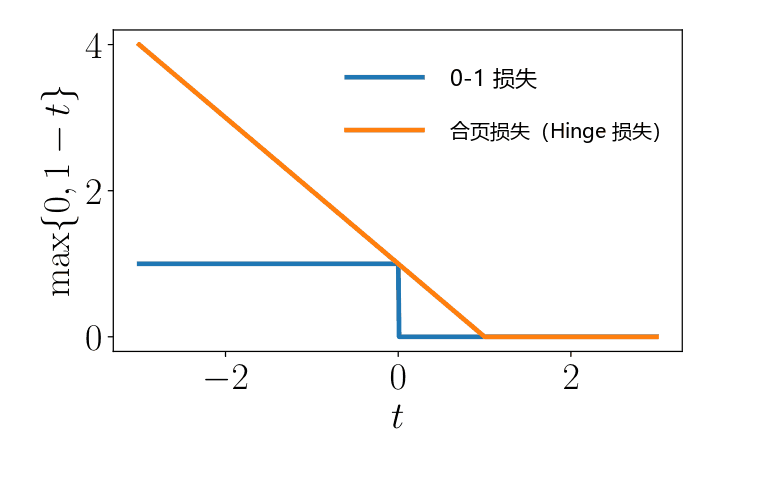
\includegraphics[width=0.92\textwidth,keepaspectratio]{docs/images/Figure12.8.png}
\caption*{图 12.8}
\end{figure}


如图 12.8 所示，合页损失可以分段表示为两个线性部分：

\begin{equation}
\ell(t) = \begin{cases} 0, & \textcn{若 } t \geqslant 1 \\ 1 - t, & \textcn{若 } t < 1 \end{cases} .
\tag{12.29}
\end{equation}

相比之下，硬间隔 SVM (12.18) 对应的等价损失函数形式为：

\begin{equation}
\ell_{\text{hard}}(t) = \begin{cases} 0, & \textcn{若 } t \geqslant 1 \\ \infty, & \textcn{若 } t < 1 \end{cases} .
\tag{12.30}
\end{equation}

这生动地表明硬间隔 SVM 绝不允许任何样本进入间隔边界内部。

对于给定的训练数据集 $ \{(\boldsymbol{x}_1, y_1), \ldots, (\boldsymbol{x}_N, y_N)\} $，我们在最小化经验风险总损失的同时引入 $ \ell_2 $ 正则化（8.2.3 节）。使用合页损失 (12.28)，我们立即得到如下无约束经验风险最小化优化问题：

\begin{equation}
\min_{\boldsymbol{w}, b} \underbrace{\frac{1}{2} \|\boldsymbol{w}\|^2}_{\textcn{正则化项}} + C \sum_{n=1}^N \underbrace{\max\{0, 1 - y_n (\langle \boldsymbol{w}, \boldsymbol{x}_n \rangle + b)\}}_{\textcn{误差项 / 损失项}} .
\tag{12.31}
\end{equation}

式 (12.31) 中的第一项正是正则化项（参见 9.2.3 节），第二项正是经验合页损失误差项。回顾 12.2.4 节可知，$ \frac{1}{2}\|\boldsymbol{w}\|^2 $ 直接源自几何间隔的倒数。换句话说，\textbf{最大化分类间隔等价于在目标函数中施加 $ \ell_2 $ 权重正则化}！

原则上，式 (12.31) 的无约束凸优化问题可以直接采用次梯度下降法（sub-gradient descent，7.1 节）求解。为了严格证明式 (12.31) 与几何软间隔 SVM (12.26a) 的等价性，注意到合页损失对单个样本的最小化：

\begin{equation}
\min_t \max\{0, 1 - t\}
\tag{12.32}
\end{equation}

可以通过引入一个辅助松弛标量 $ \xi $ 严格等价地重写为带约束的线性形式：

\begin{equation}
\min_{\xi, t} \xi \quad \text{subject to } \xi \geqslant 0, \quad \xi \geqslant 1 - t .
\tag{12.33}
\end{equation}

将这一等价变换代入式 (12.31)，令 $ t_n = y_n (\langle \boldsymbol{w}, \boldsymbol{x}_n \rangle + b) $ 并移项整理不等式约束，我们便精确复原出了软间隔 SVM 的原生优化问题 (12.26a)！

\medskip\hrule\medskip

\textbf{说明（对比线性回归的损失函数视角）} 让我们将本节中支持向量机对损失函数的选取与第 9 章线性回归的损失函数做一对比。回顾 9.2.1 节，在线性高斯假设下寻找极大似然估计时，我们通常最小化负对数似然。对于带有高斯噪声的线性回归，每个样本的负对数似然恰好是平方误差函数。因此，平方误差是极大似然解自然推导出的对应损失函数。而在 SVM 中，合页损失直接由追求大间隔与鲁棒分类的几何目标驱动而生。 ♦

\section*{12.3 对偶支持向量机}
\addcontentsline{toc}{section}{12.3 对偶支持向量机}
\label{sec:12.3}

在前几节中，我们以变量 $ \boldsymbol{w} $ 和 $ b $ 为核心所展开的描述被称为 \textbf{原生支持向量机（Primal SVM）}。回顾前文，我们考虑具有 $ D $ 个特征的输入向量 $ \boldsymbol{x} \in \mathbb{R}^D $。由于法向量 $ \boldsymbol{w} $ 与样本 $ \boldsymbol{x} $ 具有相同的维度，这意味着原生优化问题中的待估参数数量（$ \boldsymbol{w} $ 的维度）随特征维度 $ D $ 线性增长。

在接下来的内容中，我们考察一个完全等价的优化问题（即所谓的 \textbf{对偶视角（dual view）}），该问题的参数数量与特征维度完全解耦，转而随训练集中的 \textbf{样本数量 $ N $} 增长。我们在第 10 章中已经见到过类似的思想——当时我们以一种不随特征维度膨胀的方式重新表述了学习问题（10.5 节高维 PCA）。对于特征维度远大于样本数量（即 $ D \gg N $）的高维问题，这一对偶视角极其有效。此外，对偶 SVM 还有一个极为强大的额外优势：它允许极其自然且模块化地引入核方法（Kernel Methods），正如我们在本章末尾将看到的那样。“对偶（dual）”一词在数学文献中频繁出现，在当前上下文中，它特指 \textbf{凸对偶（convex duality）}。本节的核心推导本质上是我们在 7.2 节中系统讨论的凸对偶理论的经典范例。

\medskip\hrule\medskip

\section*{12.3.1 通过拉格朗日乘子法推导凸对偶}
\addcontentsline{toc}{subsection}{12.3.1 通过拉格朗日乘子法推导凸对偶}

回顾软间隔 SVM 的原生优化问题 (12.26a)。我们将对应于原生 SVM 的变量 $ \boldsymbol{w}, b, \boldsymbol{\xi} $ 统称为 \textbf{原生变量（primal variables）}。我们引入拉格朗日乘子向量：

\begin{itemize}
\item 用 $ \alpha_n \geqslant 0 $ 作为对应于正确分类不等式约束式 (12.26b) 的拉格朗日乘子；
\item 用 $ \gamma_n \geqslant 0 $ 作为对应于松弛变量非负约束式 (12.26c) 的拉格朗日乘子。
\end{itemize}

在第 7 章中，我们使用 $ \lambda $ 作为通用的拉格朗日乘子记号；而在本节中，我们遵循 SVM 领域的经典文献规范，采用 $ \alpha $ 和 $ \gamma $。由此构建的拉格朗日函数（Lagrangian）为：

\begin{equation}
\begin{adjustbox}{max width=\linewidth}
L(\boldsymbol{w}, b, \boldsymbol{\xi}, \boldsymbol{\alpha}, \boldsymbol{\gamma}) = \frac{1}{2} \|\boldsymbol{w}\|^2 + C \sum_{n=1}^N \xi_n - \sum_{n=1}^N \alpha_n \left( y_n (\langle \boldsymbol{w}, \boldsymbol{x}_n \rangle + b) - 1 + \xi_n \right) - \sum_{n=1}^N \gamma_n \xi_n .
\end{adjustbox}
\tag{12.34}
\end{equation}

为了获得对偶函数，我们分别对三个原生变量 $ \boldsymbol{w}, b $ 以及松弛分量 $ \xi_n $ 求偏导数：

\begin{equation}
\frac{\partial L}{\partial \boldsymbol{w}} = \boldsymbol{w}^\top - \sum_{n=1}^N \alpha_n y_n \boldsymbol{x}_n^\top
\tag{12.35}
\end{equation}

\begin{equation}
\frac{\partial L}{\partial b} = - \sum_{n=1}^N \alpha_n y_n
\tag{12.36}
\end{equation}

\begin{equation}
\frac{\partial L}{\partial \xi_n} = C - \alpha_n - \gamma_n .
\tag{12.37}
\end{equation}

我们通过令这三个偏导数分别等于零来求解拉格朗日函数关于原生变量的无约束极小值。首先，令式 (12.35) 为零，我们得到最优权重向量的解析表达式：

\begin{equation}
\boldsymbol{w} = \sum_{n=1}^N \alpha_n y_n \boldsymbol{x}_n
\tag{12.38}
\end{equation}

这一重要结论是现代统计学习理论中著名 \textbf{表示定理（Representer Theorem）}（Kimeldorf and Wahba, 1970）的一个具体实例。式 (12.38) 深刻表明：\textbf{原生的最优法向量 $ \boldsymbol{w} $ 可以完全由训练样本 $ \boldsymbol{x}_n $ 的线性组合来表示}。回顾 2.6.1 节，这意味着优化问题的解必然严格落入训练数据所张成的子空间（span）内。表示定理在经验风险最小化与核学习的一般理论框架下普遍成立（Hofmann et al., 2008; Argyriou and Dinuzzo, 2014）。

\medskip\hrule\medskip

\textbf{说明（“支持向量机”名称的由来）} 表示定理式 (12.38) 同时也为“支持向量机（Support Vector Machine）”这一名称提供了最本质的几何解释：那些对应拉格朗日乘子 $ \alpha_n = 0 $ 的数据样本，对最终的法向量解 $ \boldsymbol{w} $ 完全没有产生任何贡献；而那些满足 $ \alpha_n > 0 $ 的非零样本点，则直接决定并支撑着最终的分隔超平面，因此被称为 \textbf{支持向量（support vectors）}！ ♦

\medskip\hrule\medskip

接下来，将 $ \boldsymbol{w} $ 的表示式 (12.38) 代回到拉格朗日函数 (12.34) 中：

\begin{equation}
\begin{adjustbox}{max width=\linewidth}
D(\boldsymbol{\xi}, \boldsymbol{\alpha}, \boldsymbol{\gamma}) = \frac{1}{2} \sum_{i=1}^N \sum_{j=1}^N y_i y_j \alpha_i \alpha_j \langle \boldsymbol{x}_i, \boldsymbol{x}_j \rangle - \sum_{i=1}^N y_i \alpha_i \left\langle \sum_{j=1}^N y_j \alpha_j \boldsymbol{x}_j, \boldsymbol{x}_i \right\rangle + C \sum_{i=1}^N \xi_i - b \sum_{i=1}^N y_i \alpha_i + \sum_{i=1}^N \alpha_i - \sum_{i=1}^N \alpha_i \xi_i - \sum_{i=1}^N \gamma_i \xi_i .
\end{adjustbox}
\tag{12.39}
\end{equation}

仔细观察式 (12.39)：

\begin{enumerate}
\item 包含原生变量 $ \boldsymbol{w} $ 的项已经完全消除；
\item 令偏导数式 (12.36) 为零得到等式约束： $ \sum_{n=1}^N y_n \alpha_n = 0 , $ 因此包含截距 $ b $ 的项 $ b \sum_{i=1}^N y_i \alpha_i $ 恰好为 0，彻底消失；
\item 回顾 3.2 节，内积具有对称性与双线性。因此前两项展开后是对完全相同的几何对象求和，前两项合并化简为：
\end{enumerate}
\begin{equation*}
\begin{adjustbox}{max width=\linewidth}
\frac{1}{2} \sum_{i=1}^N \sum_{j=1}^N y_i y_j \alpha_i \alpha_j \langle \boldsymbol{x}_i, \boldsymbol{x}_j \rangle - \sum_{i=1}^N \sum_{j=1}^N y_i y_j \alpha_i \alpha_j \langle \boldsymbol{x}_i, \boldsymbol{x}_j \rangle = - \frac{1}{2} \sum_{i=1}^N \sum_{j=1}^N y_i y_j \alpha_i \alpha_j \langle \boldsymbol{x}_i, \boldsymbol{x}_j \rangle .
\end{adjustbox}
\end{equation*}
\begin{enumerate}
\end{enumerate}

由此，拉格朗日函数整理为：

\begin{equation}
\begin{adjustbox}{max width=\linewidth}
D(\boldsymbol{\xi}, \boldsymbol{\alpha}, \boldsymbol{\gamma}) = - \frac{1}{2} \sum_{i=1}^N \sum_{j=1}^N y_i y_j \alpha_i \alpha_j \langle \boldsymbol{x}_i, \boldsymbol{x}_j \rangle + \sum_{i=1}^N \alpha_i + \sum_{i=1}^N (C - \alpha_i - \gamma_i) \xi_i .
\end{adjustbox}
\tag{12.40}
\end{equation}

式 (12.40) 的最后一项汇总了所有包含松弛变量 $ \xi_i $ 的项。根据对 $ \xi_i $ 偏导置零的条件式 (12.37)，有 $ C - \alpha_i - \gamma_i = 0 $，因此最后一项恒为零！此外，由于乘子 $ \gamma_i \geqslant 0 $，结合 $ C - \alpha_i - \gamma_i = 0 $ 立即导出上界约束 $ \alpha_i \leqslant C $。

至此，我们成功消去了所有原生变量，导出了仅依赖于拉格朗日乘子 $ \boldsymbol{\alpha} $ 的对偶问题。回顾拉格朗日对偶性（定义 7.1），求解对偶问题对应于最大化对偶目标；这在数学上等价于最小化负的对偶函数。于是，我们得到了标准的 \textbf{对偶支持向量机（Dual SVM）} 凸二次规划问题：

\begin{equation}
\min_{\boldsymbol{\alpha}} \frac{1}{2} \sum_{i=1}^N \sum_{j=1}^N y_i y_j \alpha_i \alpha_j \langle \boldsymbol{x}_i, \boldsymbol{x}_j \rangle - \sum_{i=1}^N \alpha_i
\tag{12.41}
\end{equation}

\begin{equation*}
\text{subject to } \sum_{i=1}^N y_i \alpha_i = 0
\end{equation*}

\begin{equation*}
0 \leqslant \alpha_i \leqslant C , \quad \forall i = 1, \ldots, N .
\end{equation*}

在式 (12.41) 中：

\begin{itemize}
\item 等式约束 $ \sum_{i=1}^N y_i \alpha_i = 0 $ 源自关于截距 $ b $ 的一阶最优性条件；
\item 不等式下界 $ \alpha_i \geqslant 0 $ 源自不等式约束的拉格朗日乘子非负性（7.2 节）；
\item 不等式上界 $ \alpha_i \leqslant C $ 源自松弛变量乘子 $ \gamma_i \geqslant 0 $ 的非负性约束。
\end{itemize}

在支持向量机文献中，约束条件 $ 0 \leqslant \alpha_i \leqslant C $ 被称为 \textbf{盒约束（box constraints）}，因为它将拉格朗日乘子向量 $ \boldsymbol{\alpha} = [\alpha_1, \ldots, \alpha_N]^\top \in \mathbb{R}^N $ 限制在每个坐标轴上均介于 $ 0 $ 与 $ C $ 之间的超立方体（盒子）内部。这种坐标轴对齐的盒约束在现代凸优化数值求解器中可以被极其高效地处理（Dostál, 2009, 第 5 章）。

根据 Karush-Kuhn-Tucker (KKT) 互补松弛条件（Schölkopf and Smola, 2002）：

\begin{itemize}
\item 对于落在正确分类且在间隔边界外部的普通样本，有 $ \alpha_i = 0 $；
\item 对于恰好落在间隔超平面边界上的自由支持向量，其对偶变量严格落在盒子内部，即 $ 0 < \alpha_i < C $；
\item 对于侵入间隔内部或分类错误的受罚样本，其对偶变量达到上界，即 $ \alpha_i = C $。
\end{itemize}

一旦通过数值求解器计算出最优对偶参数 $ \boldsymbol{\alpha}^* $，我们便可利用表示定理式 (12.38) 立即恢复出原生法向量解：

\begin{equation*}
\boldsymbol{w}^* = \sum_{n=1}^N \alpha_n^* y_n \boldsymbol{x}_n .
\end{equation*}

那么，最优截距参数 $ b^* $ 该如何求解？考虑一个严格落在间隔边界上的自由支持向量样本 $ \boldsymbol{x}_n $（即满足 $ 0 < \alpha_n^* < C $ 的样本），根据定义它必然严格满足 $ \langle \boldsymbol{w}^*, \boldsymbol{x}_n \rangle + b^* = y_n $。由于 $ y_n \in \{+1, -1\} $，上式中唯一的未知数便是截距 $ b^* $，因此可直接通过下式求得：

\begin{equation}
b^* = y_n - \langle \boldsymbol{w}^*, \boldsymbol{x}_n \rangle .
\tag{12.42}
\end{equation}

\medskip\hrule\medskip

\textbf{说明（稳健计算截距 $ b^* $ 的数值技巧）} 在实际数值计算中，为了避免由于数值舍入误差带来的波动，通常会对所有满足 $ 0 < \alpha_n^* < C $ 的边界支持向量分别计算对应的 $ b $，然后取其平均值或中位数作为最终的 $ b^* $，以保证数值稳定性。 ♦

\medskip\hrule\medskip

\section*{12.3.2 对偶 SVM：凸包视角}
\addcontentsline{toc}{subsection}{12.3.2 对偶 SVM：凸包视角}

推导对偶支持向量机的另一种极具启发性的途径，是考察一个基于集合几何学的替代论证。考虑具有相同标签的样本点集，我们希望构建一个包含该类别所有样本点的 \textbf{最小凸集}。这个最小凸集被称为该点集的 \textbf{凸包（convex hull）}，如图 12.9 所示。


\begin{figure}[H]
\centering
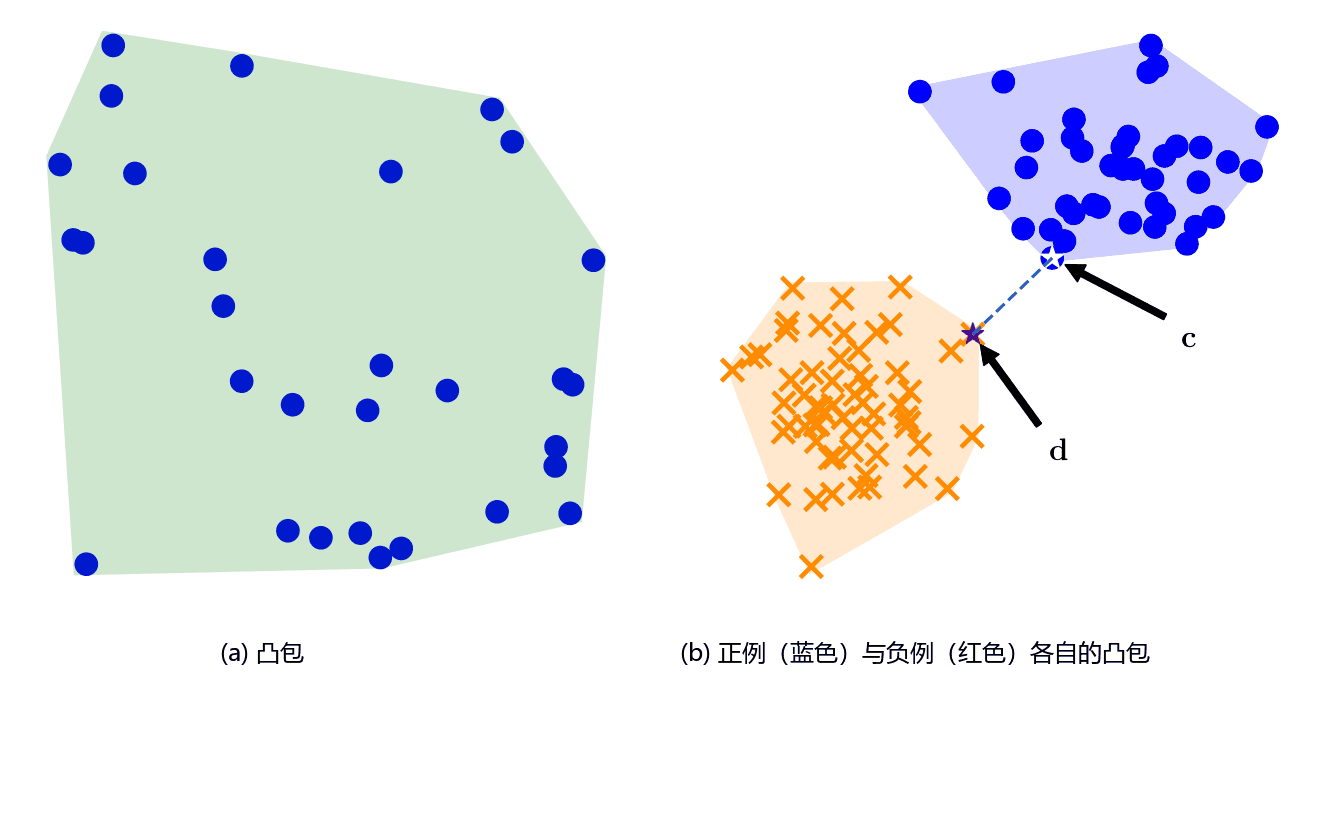
\includegraphics[width=0.92\textwidth,keepaspectratio]{docs/images/Figure12.9.png}
\caption*{图 12.9}
\end{figure}


让我们首先建立关于点集凸组合（convex combination）的直观理解：

\begin{itemize}
\item 考虑两个点 $ \boldsymbol{x}_1 $ 和 $ \boldsymbol{x}_2 $ 以及非负权重 $ \alpha_1, \alpha_2 \geqslant 0 $，且满足 $ \alpha_1 + \alpha_2 = 1 $。方程 $ \alpha_1 \boldsymbol{x}_1 + \alpha_2 \boldsymbol{x}_2 $ 精确描述了连接 $ \boldsymbol{x}_1 $ 与 $ \boldsymbol{x}_2 $ 的线段上的所有点；
\item 当我们加入第三个点 $ \boldsymbol{x}_3 $ 以及满足 $ \sum_{n=1}^3 \alpha_n = 1 $ 的非负权重 $ \alpha_3 \geqslant 0 $ 时，这三个点的凸组合张成了一个二维平面区域，其对应的凸包就是由各对顶点连接而成的三角形区域；
\item 随着我们加入更多样本点，当点的数量超过空间维度时，一部分样本点将会自然落在凸包的几何内部，如图 12.9(a) 所示。
\end{itemize}

一般地，通过为每个样本点 $ \boldsymbol{x}_n $ 引入非负权重 $ \alpha_n \geqslant 0 $，有限样本集合 $ \mathcal{X} = \{\boldsymbol{x}_1, \ldots, \boldsymbol{x}_N\} $ 的凸包可以严格定义为：

\begin{equation}
\operatorname{conv}(\mathcal{X}) = \left\{ \sum_{n=1}^N \alpha_n \boldsymbol{x}_n \ \middle|\ \sum_{n=1}^N \alpha_n = 1, \ \alpha_n \geqslant 0, \ \forall n = 1, \ldots, N \right\} .
\tag{12.43}
\end{equation}

如果对应于正类和负类的两个点云在空间中是线性可分的，那么它们各自对应的凸包 \textbf{互不重叠（do not overlap）}！

给定训练数据集 $ \{(\boldsymbol{x}_1, y_1), \ldots, (\boldsymbol{x}_N, y_N)\} $，我们分别构建正类凸包 $ \operatorname{conv}(\mathcal{X}_+) $ 和负类凸包 $ \operatorname{conv}(\mathcal{X}_-) $。现在，我们在正类凸包中选取一个点 $ \boldsymbol{c} $，在负类凸包中选取一个点 $ \boldsymbol{d} $，使得两点之间的欧几里得距离最近（参见图 12.9(b)）。我们定义两点之间的差值向量为：

\begin{equation}
\boldsymbol{w} := \boldsymbol{c} - \boldsymbol{d} .
\tag{12.44}
\end{equation}

要求点 $ \boldsymbol{c} $ 和 $ \boldsymbol{d} $ 之间的距离最近，完全等价于最小化差向量 $ \boldsymbol{w} $ 的长度（范数）：

\begin{equation}
\arg\min_{\boldsymbol{w}} \|\boldsymbol{w}\| = \arg\min_{\boldsymbol{w}} \frac{1}{2} \|\boldsymbol{w}\|^2 .
\tag{12.45}
\end{equation}

由于点 $ \boldsymbol{c} $ 属于正类凸包，它可以表示为正类样本的凸组合：

\begin{equation}
\boldsymbol{c} = \sum_{n: y_n = +1} \alpha_n^+ \boldsymbol{x}_n
\tag{12.46}
\end{equation}

其中 $ \alpha_n^+ \geqslant 0 $ 且 $ \sum_{n: y_n = +1} \alpha_n^+ = 1 $。类似地，负类凸包中的点 $ \boldsymbol{d} $ 可以表示为负类样本的凸组合：

\begin{equation}
\boldsymbol{d} = \sum_{n: y_n = -1} \alpha_n^- \boldsymbol{x}_n
\tag{12.47}
\end{equation}

其中 $ \alpha_n^- \geqslant 0 $ 且 $ \sum_{n: y_n = -1} \alpha_n^- = 1 $。将式 (12.44)、(12.46) 和 (12.47) 代入优化目标 (12.45)，我们得到：

\begin{equation}
\min_{\boldsymbol{\alpha}} \frac{1}{2} \left\| \sum_{n: y_n = +1} \alpha_n^+ \boldsymbol{x}_n - \sum_{n: y_n = -1} \alpha_n^- \boldsymbol{x}_n \right\|^2 .
\tag{12.48}
\end{equation}

令 $ \boldsymbol{\alpha} $ 为所有系数的拼接向量。由于两个凸包各自的系数和均为 1：

\begin{equation}
\sum_{n: y_n = +1} \alpha_n^+ = 1 \quad \textcn{且} \quad \sum_{n: y_n = -1} \alpha_n^- = 1 .
\tag{12.49}
\end{equation}

这自然导出了与对偶 SVM 完全相同的核心约束：

\begin{equation}
\sum_{n=1}^N y_n \alpha_n = 0 .
\tag{12.50}
\end{equation}

展开全数据集加权和可以验证这一约束：

\begin{equation}
\sum_{n=1}^N y_n \alpha_n = \sum_{n: y_n = +1} (+1) \alpha_n^+ + \sum_{n: y_n = -1} (-1) \alpha_n^-
\tag{12.51a}
\end{equation}

\begin{equation}
= \sum_{n: y_n = +1} \alpha_n^+ - \sum_{n: y_n = -1} \alpha_n^- = 1 - 1 = 0 .
\tag{12.51b}
\end{equation}

将目标函数 (12.48) 展开为关于内积的二次型，并结合约束条件 (12.50) 以及非负条件 $ \boldsymbol{\alpha} \geqslant \mathbf{0} $，我们便精确得到了与硬间隔对偶 SVM 完全等价的凸优化问题（Bennett and Bredensteiner, 2000a）！

\medskip\hrule\medskip

\textbf{说明（软间隔与约化凸包）} 对于线性不可分数据，正负两类的普通凸包会发生重叠。为了获得软间隔 SVM 的几何对偶图景，数学上引入了 \textbf{约化凸包（reduced hull）} 的概念。约化凸包在凸组合系数上增加了严格的上限约束 $ \alpha_n \leqslant C $。由于对每个顶点的最大权重进行了限制，点集无法过于集中在某些极端离群点上，从而将凸包收缩为一个体积更小、更紧凑的子凸集（Bennett and Bredensteiner, 2000b）。当两个收缩后的约化凸包不再重叠时，寻找它们之间的最近距离便精确对应于软间隔 SVM 的对偶求解！ ♦

\section*{12.4 核方法}
\addcontentsline{toc}{section}{12.4 核方法}
\label{sec:12.4}

考虑对偶支持向量机的优化公式 (12.41)。值得高度关注的是：在对偶目标函数中，内积 \textbf{仅仅出现在样本对 $ \boldsymbol{x}_i $ 与 $ \boldsymbol{x}_j $ 之间}，而完全不涉及样本与模型参数之间的内积运算。

因此，如果我们考虑使用一组特征变换 $ \boldsymbol{\phi}(\boldsymbol{x}_i) $ 来表示样本 $ \boldsymbol{x}_i $，对偶 SVM 所需进行的唯一调整就是将原有的内积进行替换。这种 \textbf{高度的模块化解耦（modularity）}——将分类方法本身（SVM 优化框架）与特征表示的选择 $ \boldsymbol{\phi}(\boldsymbol{x}) $ 完全分离——赋予了我们极其灵活的自由度，使我们能够完全独立地探索与优化这两个核心环节。在本节中，我们重点讨论特征表示 $ \boldsymbol{\phi}(\boldsymbol{x}) $ 并简要介绍 \textbf{核方法（Kernels）} 的核心思想。

由于 $ \boldsymbol{\phi}(\boldsymbol{x}) $ 可以是一个高度复杂的非线性函数，我们能够直接利用假定线性分类边界的 SVM，构造出关于原始输入样本 $ \boldsymbol{x}_n $ 具有高度非线性决策边界的强大分类器。除了软间隔之外，这为机器学习从业者处理线性不可分数据集提供了第二条极为广阔的解决路径。

在现代机器学习与统计学中，许多算法和统计方法都展现出了我们在对偶 SVM 中所观察到的这一美妙特性：\textbf{模型所需的全部数据信息均可仅通过样本之间的内积来完整表达}。

与其显式地定义一个高维甚至无限维的非线性特征映射 $ \boldsymbol{\phi}(\cdot) $ 并直接计算映射后的内积，我们可以直接定义一个度量样本 $ \boldsymbol{x}_i $ 与 $ \boldsymbol{x}_j $ 之间相似度的二元函数 $ k(\boldsymbol{x}_i, \boldsymbol{x}_j) $。对于满足特定数学条件的一类相似度函数（称为 \textbf{核函数（kernels）}），该相似度函数隐式地定义了某个再生核希尔伯特空间中的非线性特征映射 $ \boldsymbol{\phi}(\cdot) $。

\medskip\hrule\medskip

\textbf{定义（核函数）} 核函数在数学上定义为函数 $ k : \mathcal{X} \times \mathcal{X} \to \mathbb{R} $，对于该函数，存在一个希尔伯特空间 $ \mathcal{H} $ 以及特征映射 $ \boldsymbol{\phi} : \mathcal{X} \to \mathcal{H} $，使得：

\begin{equation}
k(\boldsymbol{x}_i, \boldsymbol{x}_j) = \langle \boldsymbol{\phi}(\boldsymbol{x}_i), \boldsymbol{\phi}(\boldsymbol{x}_j) \rangle_{\mathcal{H}} .
\tag{12.52}
\end{equation}

这里核函数的输入空间 $ \mathcal{X} $ 可以极其广泛，完全不局限于实数向量空间 $ \mathbb{R}^D $。

\medskip\hrule\medskip

与每一个满足条件的对称正定核函数 $ k $ 相伴的，存在一个唯一确定的 \textbf{再生核希尔伯特空间（Reproducing Kernel Hilbert Space, RKHS）}（Aronszajn, 1950; Berlinet and Thomas-Agnan, 2004）。在这个唯一对应关系中，映射 $ \boldsymbol{\phi}(\boldsymbol{x}) = k(\cdot, \boldsymbol{x}) $ 被称为 \textbf{典型特征映射（canonical feature map）}。

从直接内积计算向核函数 (12.52) 的推广在机器学习中被称为著名的 \textbf{核技巧（kernel trick）}（Schölkopf and Smola, 2002; Shawe-Taylor and Cristianini, 2004）。核技巧的核心精髓在于：它完全隐藏了显式非线性高维特征映射的具体构造与计算。

由内积或将核函数 $ k(\cdot, \cdot) $ 作用于整个训练数据集所生成的矩阵 $ \boldsymbol{K} \in \mathbb{R}^{N \times N} $ 被称为 \textbf{Gram 矩阵（Gram matrix）}，在机器学习中通常简称为 \textbf{核矩阵（kernel matrix）}。核函数必须是对称半正定的，因此由任意样本集生成的核矩阵 $ \boldsymbol{K} $ 必然是对称半正定矩阵（参见 3.2.3 节）：

\begin{equation}
\forall \boldsymbol{z} \in \mathbb{R}^N : \boldsymbol{z}^\top \boldsymbol{K} \boldsymbol{z} \geqslant 0 .
\tag{12.53}
\end{equation}


\begin{figure}[H]
\centering
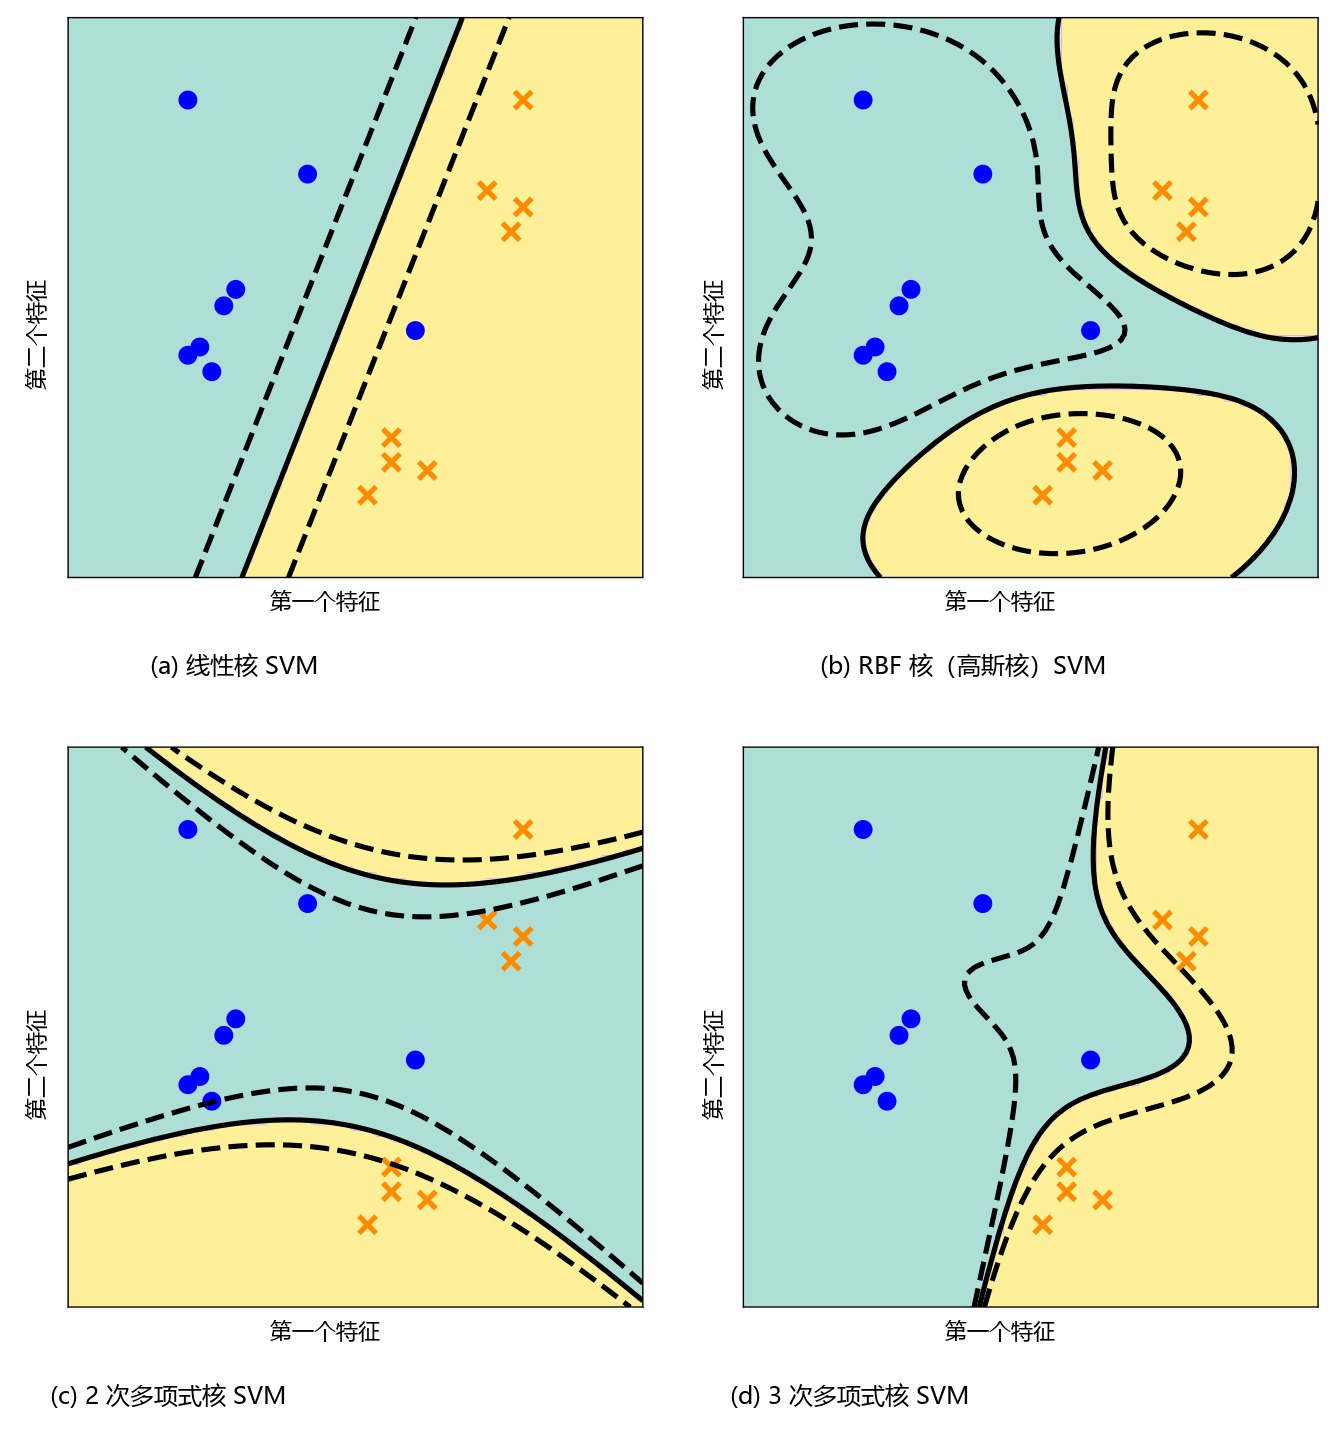
\includegraphics[width=320pt,keepaspectratio]{docs/images/Figure12.10.png}
\caption*{图 12.10}
\end{figure}


对于多元实值数据 $ \boldsymbol{x}_i \in \mathbb{R}^D $，几种最常用且最具代表性的经典核函数包括（Schölkopf and Smola, 2002; Rasmussen and Williams, 2006）：

\begin{enumerate}
\item \textbf{多项式核（Polynomial Kernel）}：$ k(\boldsymbol{x}_i, \boldsymbol{x}_j) = (\boldsymbol{x}_i^\top \boldsymbol{x}_j + c)^d $；
\item \textbf{高斯径向基函数核（Gaussian RBF Kernel，亦称高斯核）}：$ k(\boldsymbol{x}_i, \boldsymbol{x}_j) = \exp\left(-\frac{\|\boldsymbol{x}_i - \boldsymbol{x}_j\|^2}{2\sigma^2}\right) $；
\item \textbf{有理二次核（Rational Quadratic Kernel）}。
\end{enumerate}

图 12.10 直观对比了不同核函数在相同数据集上的分隔决策面表现：线性核产生笔直的线性决策面，而多项式核与高斯 RBF 核能够平滑自适应地弯曲并紧密包裹数据簇。

\medskip\hrule\medskip

\textbf{说明（关于“核（Kernel）”一词的三种不同数学含义）} 对于初入机器学习领域的学者而言，“核（Kernel）”一词在不同数学语境下具有完全不同的含义，极易产生混淆：

\begin{enumerate}
\item \textbf{再生核（Reproducing Kernel）}：在本章中，“核”特指再生核希尔伯特空间（RKHS）中的对称正定核函数（Aronszajn, 1950; Saitoh, 1988）；
\item \textbf{线性代数中的核（Kernel / Null Space）}：在 2.7.3 节的线性代数中，“核”是零空间（null space）的同义词，即满足线性变换映射为零向量的所有向量构成的子空间；
\item \textbf{核密度估计中的平滑核（Smoothing Kernel）}：在 11.5 节非参数概率密度估计中，“核”指代积分为 1 的局部平滑加权窗口函数。  
\end{enumerate}

♦

\medskip\hrule\medskip

由于显式特征表示 $ \boldsymbol{\phi}(\boldsymbol{x}) $ 在数学上与核表示 $ k(\boldsymbol{x}_i, \boldsymbol{x}_j) $ 完全等价，在实践中工程师通常优先设计能够比显式特征内积计算高效得多的核函数：

\begin{itemize}
\item 例如在 \textbf{多项式核} 中，显式展开后的单项式项数随特征维度指数级暴增（即使是低阶多项式，高维展开也是无法承受的）；而多项式核函数计算仅需先在低维执行一次内积标量运算，随后进行一次标量幂运算，带来极其显著的计算加速；
\item 在 \textbf{高斯 RBF 核} 中，其所诱导的特征空间维度在数学上是 \textbf{无穷维（infinite-dimensional）} 的！在计算机中显式存储或表达无限维向量在物理上是不可能的，但借助高斯核函数，我们只需计算一次样本间的欧氏距离和指数函数，便能在有限时间内轻而易举地完成无限维特征空间中的内积运算！
\end{itemize}

核技巧的另一个极为重大的优势在于：\textbf{输入数据根本无需预先表示为实数向量}！注意到内积仅仅定义在特征映射函数的输出值 $ \boldsymbol{\phi}(\boldsymbol{x}) \in \mathcal{H} $ 上，而对输入对象 $ \mathcal{X} $ 的类型没有施加任何实数限制。因此，核函数 $ k(\cdot, \cdot) $ 可以直接定义在任意复杂的离散或抽象非结构化对象上，例如集合、序列、文本字符串、图结构（Graph）乃至概率分布本身（Ben-Hur et al., 2008; Gärtner, 2008; Shi et al., 2009; Sriperumbudur et al., 2010; Vishwanathan et al., 2010）。在实际建模中，核函数的具体类型以及核超参数（如高斯核带宽 $ \sigma $）通常借助嵌套交叉验证（8.6.1 节）进行系统搜索与选型。

\section*{12.5 数值求解}
\addcontentsline{toc}{section}{12.5 数值求解}
\label{sec:12.5}

在结束对支持向量机的理论推导之际，我们将本章推导出的各类核心优化问题与第 7 章中介绍的数值优化概念进行系统对接。我们考察求解 SVM 最优解的两种不同数值计算路径：

\begin{enumerate}
\item \textbf{无约束损失视角}：将基于经验风险与合页损失的 SVM (8.2.2 节) 表达为无约束凸优化问题，并利用次梯度方法进行求解；
\item \textbf{带约束二次规划视角}：将原生与对偶 SVM 严格整理为标准型二次规划（Quadratic Programs, QP，7.3.2 节），以便利用现代凸优化求解器直接求解。
\end{enumerate}

\medskip\hrule\medskip

\section*{12.5.1 次梯度下降法（损失函数视角）}
\addcontentsline{toc}{subsection}{12.5.1 次梯度下降法（损失函数视角）}

考虑支持向量机的无约束经验风险目标函数 (12.31)：

\begin{equation*}
\min_{\boldsymbol{w}, b} \frac{1}{2} \|\boldsymbol{w}\|^2 + C \sum_{n=1}^N \max\{0, 1 - y_n (\langle \boldsymbol{w}, \boldsymbol{x}_n \rangle + b)\} .
\end{equation*}

这是一个关于参数 $ \boldsymbol{w} $ 和 $ b $ 的无约束凸优化问题。然而，合页损失 $ \ell(t) = \max\{0, 1 - t\} $ 在点 $ t = 1 $（即拐折处）处不可微。为此，我们需要采用 7.1 节介绍的 \textbf{次梯度（subgradient）} 方法。

合页损失几乎处处可导，唯一的非光滑奇异点仅在 $ t = 1 $ 处。在该拐点处，次微分是介于 $ 0 $ 与 $ -1 $ 之间的闭区间集合。因此，合页损失关于变量 $ t $ 的次梯度 $ g(t) \in \partial \ell(t) $ 为：

\begin{equation}
g(t) = \begin{cases} -1, & t < 1 \\ [-1, 0], & t = 1 \\ 0, & t > 1 \end{cases} .
\tag{12.54}
\end{equation}

利用该次梯度和链式法则，我们可以计算目标函数关于参数 $ \boldsymbol{w} $ 与 $ b $ 的次梯度，进而直接采用次梯度下降法（Subgradient Descent）或随机次梯度下降法（Stochastic Subgradient Descent，如著名的 Pegasos 算法，Shalev-Shwartz et al., 2011）进行数值迭代优化。

\medskip\hrule\medskip

\section*{12.5.2 标准二次规划求解（原生与对偶形式）}
\addcontentsline{toc}{subsection}{12.5.2 标准二次规划求解（原生与对偶形式）}

原生 SVM 与对偶 SVM 均严格属于 \textbf{凸二次规划问题（Convex Quadratic Programming）}。回顾原生 SVM 式 (12.26a)，其优化变量的维度取决于输入样本的特征维度 $ D $；而对偶 SVM 式 (12.41) 的优化变量维度则完全由样本容量 $ N $ 决定。

\subsection*{1. 原生软间隔 SVM 的标准矩阵形式}
\addcontentsline{toc}{subsubsection}{1. 原生软间隔 SVM 的标准矩阵形式}

回顾式 (7.45) 中的标准二次规划形式：

\begin{equation*}
\min_{\boldsymbol{z}} \frac{1}{2} \boldsymbol{z}^\top \boldsymbol{Q} \boldsymbol{z} + \boldsymbol{c}^\top \boldsymbol{z} \quad \text{subject to } \boldsymbol{A} \boldsymbol{z} \leqslant \boldsymbol{b} .
\end{equation*}

为了将原生软间隔 SVM (12.26a) 表达为标准型，我们将不等式约束移项，统一转换为“小于等于”形式：

\begin{equation}
\min_{\boldsymbol{w}, b, \boldsymbol{\xi}} \frac{1}{2} \|\boldsymbol{w}\|^2 + C \sum_{n=1}^N \xi_n
\tag{12.55}
\end{equation}

\begin{equation*}
\text{subject to } - y_n \boldsymbol{x}_n^\top \boldsymbol{w} - y_n b - \xi_n \leqslant -1 , \quad -\xi_n \leqslant 0 , \quad \forall n = 1, \ldots, N .
\end{equation*}

将变量拼接为联合参数向量 $ \boldsymbol{z} = [\boldsymbol{w}^\top, b, \boldsymbol{\xi}^\top]^\top \in \mathbb{R}^{D + 1 + N} $，通过仔细整理各项矩阵分块，我们得到原生软间隔 SVM 的分块矩阵标准形式：

\begin{equation}
\begin{adjustbox}{max width=\linewidth}
\min_{\boldsymbol{w}, b, \boldsymbol{\xi}} \frac{1}{2} \begin{bmatrix} \boldsymbol{w} \\ b \\ \boldsymbol{\xi} \end{bmatrix}^\top \begin{bmatrix} \boldsymbol{I}_D & \mathbf{0}_{D, N+1} \\ \mathbf{0}_{N+1, D} & \mathbf{0}_{N+1, N+1} \end{bmatrix} \begin{bmatrix} \boldsymbol{w} \\ b \\ \boldsymbol{\xi} \end{bmatrix} + \begin{bmatrix} \mathbf{0}_{D+1, 1} \\ C \mathbf{1}_{N, 1} \end{bmatrix}^\top \begin{bmatrix} \boldsymbol{w} \\ b \\ \boldsymbol{\xi} \end{bmatrix}
\end{adjustbox}
\tag{12.56}
\end{equation}

\begin{equation*}
\begin{adjustbox}{max width=\linewidth}
\text{subject to } \begin{bmatrix} -\boldsymbol{Y}\boldsymbol{X} & -\boldsymbol{y} & -\boldsymbol{I}_N \\ \mathbf{0}_{N, D+1} & & -\boldsymbol{I}_N \end{bmatrix} \begin{bmatrix} \boldsymbol{w} \\ b \\ \boldsymbol{\xi} \end{bmatrix} \leqslant \begin{bmatrix} -\mathbf{1}_{N, 1} \\ \mathbf{0}_{N, 1} \end{bmatrix} .
\end{adjustbox}
\end{equation*}

在上述分块矩阵表示中：

\begin{itemize}
\item $ \boldsymbol{I}_m $ 表示 $ m \times m $ 的单位矩阵；
\item $ \mathbf{0}_{m, n} $ 表示 $ m \times n $ 的全零矩阵；
\item $ \mathbf{1}_{m, n} $ 表示 $ m \times n $ 的全 1 矩阵；
\item $ \boldsymbol{y} = [y_1, \ldots, y_N]^\top \in \mathbb{R}^N $ 为标签列向量；
\item $ \boldsymbol{Y} = \operatorname{diag}(\boldsymbol{y}) \in \mathbb{R}^{N \times N} $ 是以各样本标签为主对角线元素的对角矩阵；
\item $ \boldsymbol{X} \in \mathbb{R}^{N \times D} $ 是按行拼接所有训练样本所构成的数据设计矩阵。
\end{itemize}

\medskip\hrule\medskip

\subsection*{2. 对偶 SVM 的标准矩阵形式}
\addcontentsline{toc}{subsubsection}{2. 对偶 SVM 的标准矩阵形式}

类似地，我们可以将对偶 SVM (12.41) 整理为标准二次规划形式。首先定义核矩阵 $ \boldsymbol{K} \in \mathbb{R}^{N \times N} $，其元素为 $ K_{ij} = k(\boldsymbol{x}_i, \boldsymbol{x}_j) $（对于显式线性特征，即 $ K_{ij} = \langle \boldsymbol{x}_i, \boldsymbol{x}_j \rangle $）。

利用标签对角阵 $ \boldsymbol{Y} = \operatorname{diag}(\boldsymbol{y}) $，对偶目标中的二次项紧凑写作：

\begin{equation*}
\sum_{i=1}^N \sum_{j=1}^N y_i y_j \alpha_i \alpha_j K_{ij} = \boldsymbol{\alpha}^\top \boldsymbol{Y} \boldsymbol{K} \boldsymbol{Y} \boldsymbol{\alpha} .
\end{equation*}

对偶 SVM 的标准矩阵二次规划形式为：

\begin{equation}
\min_{\boldsymbol{\alpha}} \frac{1}{2} \boldsymbol{\alpha}^\top \boldsymbol{Y} \boldsymbol{K} \boldsymbol{Y} \boldsymbol{\alpha} - \mathbf{1}_{N, 1}^\top \boldsymbol{\alpha}
\tag{12.57}
\end{equation}

\begin{equation*}
\begin{adjustbox}{max width=\linewidth}
\text{subject to } \begin{bmatrix} \boldsymbol{y}^\top \\ -\boldsymbol{y}^\top \\ -\boldsymbol{I}_N \\ \boldsymbol{I}_N \end{bmatrix} \boldsymbol{\alpha} \leqslant \begin{bmatrix} \mathbf{0}_{N+2, 1} \\ C \mathbf{1}_{N, 1} \end{bmatrix} .
\end{adjustbox}
\end{equation*}

\medskip\hrule\medskip

\textbf{说明（将等式约束转换为标准不等式约束）} 在 7.3.1 和 7.3.2 节中，标准二次规划的约束被统一规范为不等式约束。对偶 SVM 中的标量等式约束 $ \boldsymbol{y}^\top \boldsymbol{\alpha} = 0 $ 在式 (12.57) 中被拆解为两个相反方向的紧不等式：

\begin{equation}
\boldsymbol{A}\boldsymbol{x} = \boldsymbol{b} \iff \boldsymbol{A}\boldsymbol{x} \leqslant \boldsymbol{b} \quad \textcn{且} \quad -\boldsymbol{A}\boldsymbol{x} \leqslant -\boldsymbol{b} .
\tag{12.58}
\end{equation}

在实际优化软件中，大部分成熟的二次规划求解器原生支持直接输入等式约束与变量边界约束（box constraints），无需显式做此拆解。 ♦

\medskip\hrule\medskip

尽管在此处我们将 SVM 表达为标准凸二次规划形式，但在实际大规模工业界实践中，直接调用通用稠密二次规划求解器并不是最高效的方案（因为存储 $ N \times N $ 的核矩阵需要 $ \mathcal{O}(N^2) $ 的内存，求解通用 QP 复杂度通常高达 $ \mathcal{O}(N^3) $）。最著名的专用 SVM 开源求解器（如台湾大学林智仁团队开发的 \textbf{LIBSVM}（Chang and Lin, 2011）以及 Thorsten Joachims 开发的 \textbf{SVMlight}（Joachims, 1999））主要采用 \textbf{序列最小最优化算法（Sequential Minimal Optimization, SMO）}。SMO 算法在每次迭代中仅选取两个拉格朗日乘子进行解析求解，彻底避免了大矩阵存储与求逆，使得核化支持向量机能够高效处理大规模实际数据集（Platt, 1998; Nocedal and Wright, 2006; Shawe-Taylor and Sun, 2011）。

\section*{12.6 延伸阅读}
\addcontentsline{toc}{section}{12.6 延伸阅读}
\label{sec:12.6}

支持向量机只是研究二元分类问题的众多机器学习算法之一。在统计学习与模式识别领域，其他广泛使用的经典分类方法还包括感知机（perceptron）、对数几率回归（logistic regression，俗称逻辑回归）、Fisher 线性判别（Fisher discriminant）、$ k $-近邻法（$ k $-nearest neighbor, $ k $-NN）、朴素贝叶斯（naive Bayes）以及随机森林（random forest）等（Bishop, 2006; Murphy, 2012）。关于序列数据上核方法与 SVM 的系统教程可参阅 Ben-Hur 等人（2008）的综述。

支持向量机的诞生与演进同 \textbf{经验风险最小化（Empirical Risk Minimization, ERM）}（8.2 节）紧密相连。正因如此，SVM 具有坚实深厚的统计学习理论保障（Vapnik, 2000; Steinwart and Christmann, 2008）。关于核方法的权威专著当属 Schölkopf and Smola（2002）的经典名著，该书极其详尽地阐述了支持向量机的数学结构与数值最优化策略。Shawe-Taylor and Cristianini（2004）的专著则站在更广阔的视角，系统介绍了结合线性代数解决各类复杂机器学习问题的核方法体系。

推导对偶 SVM 的另一条重要数学路径是借助 \textbf{Legendre-Fenchel 变换（凸共轭）}（参见 7.3.3 节）。这一推导将 SVM 的无约束经验风险目标 (12.31) 中的每一项分别独立拆解，并精细计算其对应的凸共轭函数（Rifkin and Lippert, 2007）。对从泛函分析与正则化理论视角研究 SVM 感兴趣的读者，推荐深入研读 Grace Wahba（1990）的奠基性专著。再生核理论的严格泛函展开（Aronszajn, 1950; Schwartz, 1964; Saitoh, 1988; Manton and Amblard, 2015）需要读者具备坚实的线性算子理论基础（Akhiezer and Glazman, 1993）。近年来，核方法的数学基础已经被进一步推广至巴拿赫空间（Banach spaces, Zhang et al., 2009）以及不定内积克莱因空间（Kreĭn spaces, Ong et al., 2004; Loosli et al., 2016）。

回顾前文，合页损失（hinge loss）具有三种在数学上完全等价的表述形式：

\begin{enumerate}
\item \textbf{紧凑极大值形式}：$ \ell(t) = \max\{0, 1 - t\} $（式 (12.28)），该形式最常用于与其他常见凸损失函数（如对数损失、指数损失）进行统计风险与代偿不等式对比（Steinwart, 2007）；
\item \textbf{两段分段线性形式}：式 (12.29)，由于每一段均为严格线性，该形式最便于计算次梯度（12.5.1 节）；
\item \textbf{带松弛变量的约束形式}：式 (12.33)，该形式直接赋予了我们运用标准凸二次规划（QP）求解器（7.3.2 节）的能力。
\end{enumerate}

因为二元分类是机器学习中研究最为透彻的基础任务，在不同文献中也经常使用诸如判别（discrimination）、分隔（separation）和决策（decision）等术语。此外，二元分类器的最终输出在实际系统中通常存在三种不同层次的表达：

\begin{enumerate}
\item \textbf{原始线性评分（Score）}：线性函数本身的直接输出 $ f(\boldsymbol{x}) = \langle \boldsymbol{w}, \boldsymbol{x} \rangle + b $，其取值为任意实数。该数值的大小直接反映了分类的确信程度，常用于对样本进行排序（Ranking），此时二元分类可等价视为在排序序列上挑选最优阈值（Shawe-Taylor and Cristianini, 2004）；
\item \textbf{校准类概率估计（Class Probability Estimation）}：将原始评分通过非线性单调映射函数压缩至 $ [0, 1] $ 区间内。最常用的非线性映射是 Sigmoid（Logistic）函数（Bishop, 2006）。当映射经过良好校准后（Gneiting and Raftery, 2007; Reid and Williamson, 2011），输出可被严格解释为后验条件概率 $ P(Y = +1 \mid \boldsymbol{X} = \boldsymbol{x}) $；
\item \textbf{确定性离散决策（Binary Decision）}：取输出的符号判定 $ \hat{y} \in \{+1, -1\} $，这是分类任务最传统通用的输出形态。
\end{enumerate}

标准支持向量机本质上是确定性几何分类器，其本身并不直接具备自然的概率解释。为了将 SVM 的原始实值评分转换为校准良好的后验概率估计，工业界广泛采用由 John Platt 提出的后验概率拟合技术（\textbf{Platt 缩放，Platt Scaling}，Platt, 2000; Zadrozny and Elkan, 2001; Lin et al., 2007）。

从概率建模与训练的视角来看，存在诸多与 SVM 紧密呼应的概率分类模型。正如我们在 12.2.5 节末尾所指出的，损失函数与似然函数之间存在深刻的对应关系（可对照 8.2 节与 8.3 节）：在训练过程中对线性输出施加校准的极大似然分类模型正是 \textbf{对数几率回归（Logistic Regression）}，它属于广义线性模型（Generalized Linear Models, GLM）的范畴（Agresti, 2002, 第 5 章; McCullagh and Nelder, 1989, 第 4 章）。自然地，我们可以在贝叶斯框架下通过推断参数的后验分布来构建 \textbf{贝叶斯对数几率回归（Bayesian Logistic Regression）}，这涉及到先验分布的选择与共轭近似设计（6.6.1 节）。进一步地，如果我们将隐函数本身置于无限维高斯过程先验之下，便直接导出了极其强大的非参数贝叶斯分类模型——\textbf{高斯过程分类（Gaussian Process Classification, GPC）}（Rasmussen and Williams, 2006, 第 3 章）。


\backmatter

\chapter*{参考文献 (References)}
\addcontentsline{toc}{section}{参考文献 (References)}

本书涉及的所有学术专著、经典论文及技术报告的完整参考文献列表如下：

\begin{enumerate}
\item Abel, Niels H. 1826. Démonstration de l’Impossibilité de la Résolution Algébrique des Équations Générales qui Passent le Quatrième Degré. Grøndahl and Søn.
\end{enumerate}

\begin{enumerate}
\item Adhikari, Ani, and DeNero, John. 2018. Computational and Inferential Thinking: The Foundations of Data Science. Gitbooks.
\end{enumerate}

\begin{enumerate}
\item Agarwal, Arvind, and Daumé III, Hal. 2010. A Geometric View of Conjugate Priors. Machine Learning, 81(1), 99–113.
\end{enumerate}

\begin{enumerate}
\item Agresti, A. 2002. Categorical Data Analysis. Wiley.
\end{enumerate}

\begin{enumerate}
\item Akaike, Hirotugu. 1974. A New Look at the Statistical Model Identification. IEEE Transactions on Automatic Control, 19(6), 716–723.
\end{enumerate}

\begin{enumerate}
\item Akhiezer, Naum I., and Glazman, Izrail M. 1993. Theory of Linear Operators in Hilbert Space. Dover Publications.
\end{enumerate}

\begin{enumerate}
\item Alpaydin, Ethem. 2010. Introduction to Machine Learning. MIT Press.
\end{enumerate}

\begin{enumerate}
\item Amari, Shun-ichi. 2016. Information Geometry and Its Applications. Springer.
\end{enumerate}

\begin{enumerate}
\item Argyriou, Andreas, and Dinuzzo, Francesco. 2014. A Unifying View of Representer Theorems. In: Proceedings of the International Conference on Machine Learning.
\end{enumerate}

\begin{enumerate}
\item Aronszajn, Nachman. 1950. Theory of Reproducing Kernels. Transactions of the Amer- ican Mathematical Society, 68, 337–404.
\end{enumerate}

\begin{enumerate}
\item Axler, Sheldon. 2015. Linear Algebra Done Right. Springer. Bakir, Gökhan, Hofmann, Thomas, Schölkopf, Bernhard, Smola, Alexander J., Taskar,
\end{enumerate}

\begin{enumerate}
\item Ben, and Vishwanathan, S. V. N. (eds). 2007. Predicting Structured Data. MIT Press.
\end{enumerate}

\begin{enumerate}
\item Barber, David. 2012. Bayesian Reasoning and Machine Learning. Cambridge University Press.
\end{enumerate}

\begin{enumerate}
\item Barndorff-Nielsen, Ole. 2014. Information and Exponential Families: In Statistical The- ory. Wiley.
\end{enumerate}

\begin{enumerate}
\item Bartholomew, David, Knott, Martin, and Moustaki, Irini. 2011. Latent Variable Models and Factor Analysis: A Unified Approach. Wiley. Baydin, Atılım G., Pearlmutter, Barak A., Radul, Alexey A., and Siskind, Jeffrey M. 2018. Automatic Differentiation in Machine Learning: A Survey. Journal of Machine Learning Research, 18, 1–43.
\end{enumerate}

\begin{enumerate}
\item Beck, Amir, and Teboulle, Marc. 2003. Mirror Descent and Nonlinear Projected Subgra- dient Methods for Convex Optimization. Operations Research Letters, 31(3), 167– 175.
\end{enumerate}

\begin{enumerate}
\item Belabbas, Mohamed-Ali, and Wolfe, Patrick J. 2009. Spectral Methods in Machine Learning and New Strategies for Very Large Datasets. Proceedings of the National Academy of Sciences, 0810600105.
\end{enumerate}

\begin{enumerate}
\item Belkin, Mikhail, and Niyogi, Partha. 2003. Laplacian Eigenmaps for Dimensionality Reduction and Data Representation. Neural Computation, 15(6), 1373–1396. Ben-Hur, Asa, Ong, Cheng Soon, Sonnenburg, Sören, Schölkopf, Bernhard, and Rätsch, Gunnar. 2008. Support Vector Machines and Kernels for Computational Biology. PLoS Computational Biology, 4(10), e1000173. This material will be published by Cambridge University Press as Mathematics for Machine Learn- ing by Marc Peter Deisenroth, A. Aldo Faisal, and Cheng Soon Ong. This pre-publication version is free to view and download for personal use only. Not for re-distribution, re-sale or use in deriva- Bennett, Kristin P., and Bredensteiner, Erin J. 2000a. Duality and Geometry in SVM Classifiers. In: Proceedings of the International Conference on Machine Learning. Bennett, Kristin P., and Bredensteiner, Erin J. 2000b. Geometry in Learning. Pages 132–145 of: Geometry at Work. Mathematical Association of America.
\end{enumerate}

\begin{enumerate}
\item Berlinet, Alain, and Thomas-Agnan, Christine. 2004. Reproducing Kernel Hilbert Spaces in Probability and Statistics. Springer.
\end{enumerate}

\begin{enumerate}
\item Bertsekas, Dimitri P. 1999. Nonlinear Programming. Athena Scientific.
\end{enumerate}

\begin{enumerate}
\item Bertsekas, Dimitri P. 2009. Convex Optimization Theory. Athena Scientific.
\end{enumerate}

\begin{enumerate}
\item Bickel, Peter J., and Doksum, Kjell. 2006. Mathematical Statistics, Basic Ideas and Selected Topics. Vol. 1. Prentice Hall.
\end{enumerate}

\begin{enumerate}
\item Bickson, Danny, Dolev, Danny, Shental, Ori, Siegel, Paul H., and Wolf, Jack K. 2007. Linear Detection via Belief Propagation. In: Proceedings of the Annual Allerton Con- ference on Communication, Control, and Computing.
\end{enumerate}

\begin{enumerate}
\item Billingsley, Patrick. 1995. Probability and Measure. Wiley.
\end{enumerate}

\begin{enumerate}
\item Bishop, Christopher M. 1995. Neural Networks for Pattern Recognition. Clarendon Press.
\end{enumerate}

\begin{enumerate}
\item Bishop, Christopher M. 1999. Bayesian PCA. In: Advances in Neural Information Pro- cessing Systems.
\end{enumerate}

\begin{enumerate}
\item Bishop, Christopher M. 2006. Pattern Recognition and Machine Learning. Springer.
\end{enumerate}

\begin{enumerate}
\item Blei, David M., Kucukelbir, Alp, and McAuliffe, Jon D. 2017. Variational Inference: A Review for Statisticians. Journal of the American Statistical Association, 112(518), 859–877.
\end{enumerate}

\begin{enumerate}
\item Blum, Arvim, and Hardt, Moritz. 2015. The Ladder: A Reliable Leaderboard for Ma- chine Learning Competitions. In: International Conference on Machine Learning. Bonnans, J. Frédéric, Gilbert, J. Charles, Lemaréchal, Claude, and Sagastizábal, Clau- dia A. 2006. Numerical Optimization: Theoretical and Practical Aspects. Springer.
\end{enumerate}

\begin{enumerate}
\item Borwein, Jonathan M., and Lewis, Adrian S. 2006. Convex Analysis and Nonlinear Optimization. 2nd edn. Canadian Mathematical Society.
\end{enumerate}

\begin{enumerate}
\item Bottou, Léon. 1998. Online Algorithms and Stochastic Approximations. Pages 9–42 of: Online Learning and Neural Networks. Cambridge University Press.
\end{enumerate}

\begin{enumerate}
\item Bottou, Léon, Curtis, Frank E., and Nocedal, Jorge. 2018. Optimization Methods for Large-Scale Machine Learning. SIAM Review, 60(2), 223–311.
\end{enumerate}

\begin{enumerate}
\item Boucheron, Stephane, Lugosi, Gabor, and Massart, Pascal. 2013. Concentration In- equalities: A Nonasymptotic Theory of Independence. Oxford University Press.
\end{enumerate}

\begin{enumerate}
\item Boyd, Stephen, and Vandenberghe, Lieven. 2004. Convex Optimization. Cambridge University Press.
\end{enumerate}

\begin{enumerate}
\item Boyd, Stephen, and Vandenberghe, Lieven. 2018. Introduction to Applied Linear Alge- bra. Cambridge University Press.
\end{enumerate}

\begin{enumerate}
\item Brochu, Eric, Cora, Vlad M., and de Freitas, Nando. 2009. A Tutorial on Bayesian Optimization of Expensive Cost Functions, with Application to Active User Modeling and Hierarchical Reinforcement Learning. Tech. rept. TR-2009-023. Department of Computer Science, University of British Columbia.
\end{enumerate}

\begin{enumerate}
\item Brooks, Steve, Gelman, Andrew, Jones, Galin L., and Meng, Xiao-Li (eds). 2011. Hand- book of Markov Chain Monte Carlo. Chapman and Hall/CRC.
\end{enumerate}

\begin{enumerate}
\item Brown, Lawrence D. 1986. Fundamentals of Statistical Exponential Families: With Ap- plications in Statistical Decision Theory. Institute of Mathematical Statistics.
\end{enumerate}

\begin{enumerate}
\item Bryson, Arthur E. 1961. A Gradient Method for Optimizing Multi-Stage Allocation Processes. In: Proceedings of the Harvard University Symposium on Digital Computers and Their Applications.
\end{enumerate}

\begin{enumerate}
\item Bubeck, Sébastien. 2015. Convex Optimization: Algorithms and Complexity. Founda- tions and Trends in Machine Learning, 8(3-4), 231–357. Bühlmann, Peter, and Van De Geer, Sara. 2011. Statistics for High-Dimensional Data. Springer.
\end{enumerate}

\begin{enumerate}
\item Burges, Christopher. 2010. Dimension Reduction: A Guided Tour. Foundations and Trends in Machine Learning, 2(4), 275–365.
\end{enumerate}

\begin{enumerate}
\item Carroll, J Douglas, and Chang, Jih-Jie. 1970. Analysis of Individual Differences in Multidimensional Scaling via an N-Way Generalization of “Eckart-Young” Decom- position. Psychometrika, 35(3), 283–319.
\end{enumerate}

\begin{enumerate}
\item Casella, George, and Berger, Roger L. 2002. Statistical Inference. Duxbury. C¸inlar, Erhan. 2011. Probability and Stochastics. Springer.
\end{enumerate}

\begin{enumerate}
\item Chang, Chih-Chung, and Lin, Chih-Jen. 2011. LIBSVM: A Library for Support Vector Machines. ACM Transactions on Intelligent Systems and Technology, 2, 27:1–27:27.
\end{enumerate}

\begin{enumerate}
\item Cheeseman, Peter. 1985. In Defense of Probability. In: Proceedings of the International Joint Conference on Artificial Intelligence.
\end{enumerate}

\begin{enumerate}
\item Chollet, Francois, and Allaire, J. J. 2018. Deep Learning with R. Manning Publications.
\end{enumerate}

\begin{enumerate}
\item Codd, Edgar F. 1990. The Relational Model for Database Management. Addison-Wesley Longman Publishing.
\end{enumerate}

\begin{enumerate}
\item Cunningham, John P., and Ghahramani, Zoubin. 2015. Linear Dimensionality Reduc- tion: Survey, Insights, and Generalizations. Journal of Machine Learning Research, 16, 2859–2900.
\end{enumerate}

\begin{enumerate}
\item Datta, Biswa N. 2010. Numerical Linear Algebra and Applications. SIAM.
\end{enumerate}

\begin{enumerate}
\item Davidson, Anthony C., and Hinkley, David V. 1997. Bootstrap Methods and Their Appli- cation. Cambridge University Press.
\end{enumerate}

\begin{enumerate}
\item Dean, Jeffrey, Corrado, Greg S., Monga, Rajat, and Chen, et al. 2012. Large Scale Distributed Deep Networks. In: Advances in Neural Information Processing Systems.
\end{enumerate}

\begin{enumerate}
\item Deisenroth, Marc P., and Mohamed, Shakir. 2012. Expectation Propagation in Gaus- sian Process Dynamical Systems. Pages 2618–2626 of: Advances in Neural Informa- tion Processing Systems.
\end{enumerate}

\begin{enumerate}
\item Deisenroth, Marc P., and Ohlsson, Henrik. 2011. A General Perspective on Gaussian Filtering and Smoothing: Explaining Current and Deriving New Algorithms. In: Proceedings of the American Control Conference.
\end{enumerate}

\begin{enumerate}
\item Deisenroth, Marc P., Fox, Dieter, and Rasmussen, Carl E. 2015. Gaussian Processes for Data-Efficient Learning in Robotics and Control. IEEE Transactions on Pattern Analysis and Machine Intelligence, 37(2), 408–423.
\end{enumerate}

\begin{enumerate}
\item Dempster, Arthur P., Laird, Nan M., and Rubin, Donald B. 1977. Maximum Likelihood from Incomplete Data via the EM Algorithm. Journal of the Royal Statistical Society, 39(1), 1–38. Deng, Li, Seltzer, Michael L., Yu, Dong, Acero, Alex, Mohamed, Abdel-rahman, and
\end{enumerate}

\begin{enumerate}
\item Hinton, Geoffrey E. 2010. Binary Coding of Speech Spectrograms Using a Deep Auto-Encoder. In: Proceedings of Interspeech.
\end{enumerate}

\begin{enumerate}
\item Devroye, Luc. 1986. Non-Uniform Random Variate Generation. Springer.
\end{enumerate}

\begin{enumerate}
\item Donoho, David L., and Grimes, Carrie. 2003. Hessian Eigenmaps: Locally Linear Embedding Techniques for High-Dimensional Data. Proceedings of the National Academy of Sciences, 100(10), 5591–5596.
\end{enumerate}

\begin{enumerate}
\item Dostál, Zden˘ek. 2009. Optimal Quadratic Programming Algorithms: With Applications to Variational Inequalities. Springer.
\end{enumerate}

\begin{enumerate}
\item Douven, Igor. 2017. Abduction. In: The Stanford Encyclopedia of Philosophy. Meta- physics Research Lab, Stanford University.
\end{enumerate}

\begin{enumerate}
\item Downey, Allen B. 2014. Think Stats: Exploratory Data Analysis. 2nd edn. O’Reilly Media.
\end{enumerate}

\begin{enumerate}
\item Dreyfus, Stuart. 1962. The Numerical Solution of Variational Problems. Journal of Mathematical Analysis and Applications, 5(1), 30–45.
\end{enumerate}

\begin{enumerate}
\item Drumm, Volker, and Weil, Wolfgang. 2001. Lineare Algebra und Analytische Geometrie. Lecture Notes, Universität Karlsruhe (TH).
\end{enumerate}

\begin{enumerate}
\item Dudley, Richard M. 2002. Real Analysis and Probability. Cambridge University Press.
\end{enumerate}

\begin{enumerate}
\item Eaton, Morris L. 2007. Multivariate Statistics: A Vector Space Approach. Institute of Mathematical Statistics Lecture Notes.
\end{enumerate}

\begin{enumerate}
\item Eckart, Carl, and Young, Gale. 1936. The Approximation of One Matrix by Another of Lower Rank. Psychometrika, 1(3), 211–218.
\end{enumerate}

\begin{enumerate}
\item Efron, Bradley, and Hastie, Trevor. 2016. Computer Age Statistical Inference: Algorithms, Evidence and Data Science. Cambridge University Press.
\end{enumerate}

\begin{enumerate}
\item Efron, Bradley, and Tibshirani, Robert J. 1993. An Introduction to the Bootstrap. Chap- man and Hall/CRC.
\end{enumerate}

\begin{enumerate}
\item Elliott, Conal. 2009. Beautiful Differentiation. In: International Conference on Func- tional Programming.
\end{enumerate}

\begin{enumerate}
\item Evgeniou, Theodoros, Pontil, Massimiliano, and Poggio, Tomaso. 2000. Statistical Learning Theory: A Primer. International Journal of Computer Vision, 38(1), 9–13. Fan, Rong-En, Chang, Kai-Wei, Hsieh, Cho-Jui, Wang, Xiang-Rui, and Lin, Chih-Jen. 2008. LIBLINEAR: A Library for Large Linear Classification. Journal of Machine Learning Research, 9, 1871–1874.
\end{enumerate}

\begin{enumerate}
\item Gal, Yarin, van der Wilk, Mark, and Rasmussen, Carl E. 2014. Distributed Variational Inference in Sparse Gaussian Process Regression and Latent Variable Models. In: Advances in Neural Information Processing Systems. Gärtner, Thomas. 2008. Kernels for Structured Data. World Scientific.
\end{enumerate}

\begin{enumerate}
\item Gavish, Matan, and Donoho, David L. 2014. The Optimal Hard Threshold for Singular Values is 4 √ 3. IEEE Transactions on Information Theory, 60(8), 5040–5053.
\end{enumerate}

\begin{enumerate}
\item Gelman, Andrew, Carlin, John B., Stern, Hal S., and Rubin, Donald B. 2004. Bayesian Data Analysis. Chapman and Hall/CRC.
\end{enumerate}

\begin{enumerate}
\item Gentle, James E. 2004. Random Number Generation and Monte Carlo Methods. Springer.
\end{enumerate}

\begin{enumerate}
\item Ghahramani, Zoubin. 2015. Probabilistic Machine Learning and Artificial Intelligence. Nature, 521, 452–459.
\end{enumerate}

\begin{enumerate}
\item Ghahramani, Zoubin, and Roweis, Sam T. 1999. Learning Nonlinear Dynamical Sys- tems Using an EM Algorithm. In: Advances in Neural Information Processing Systems. MIT Press.
\end{enumerate}

\begin{enumerate}
\item Gilks, Walter R., Richardson, Sylvia, and Spiegelhalter, David J. 1996. Markov Chain Monte Carlo in Practice. Chapman and Hall/CRC.
\end{enumerate}

\begin{enumerate}
\item Gneiting, Tilmann, and Raftery, Adrian E. 2007. Strictly Proper Scoring Rules, Pre- diction, and Estimation. Journal of the American Statistical Association, 102(477), 359–378.
\end{enumerate}

\begin{enumerate}
\item Goh, Gabriel. 2017. Why Momentum Really Works. Distill.
\end{enumerate}

\begin{enumerate}
\item Gohberg, Israel, Goldberg, Seymour, and Krupnik, Nahum. 2012. Traces and Determi- nants of Linear Operators. Birkhäuser.
\end{enumerate}

\begin{enumerate}
\item Golan, Jonathan S. 2007. The Linear Algebra a Beginning Graduate Student Ought to Know. Springer.
\end{enumerate}

\begin{enumerate}
\item Golub, Gene H., and Van Loan, Charles F. 2012. Matrix Computations. JHU Press.
\end{enumerate}

\begin{enumerate}
\item Goodfellow, Ian, Bengio, Yoshua, and Courville, Aaron. 2016. Deep Learning. MIT Press. Graepel, Thore, Candela, Joaquin Quiñonero-Candela, Borchert, Thomas, and Her- brich, Ralf. 2010. Web-Scale Bayesian Click-through Rate Prediction for Sponsored Search Advertising in Microsoft’s Bing Search Engine. In: Proceedings of the Interna- tional Conference on Machine Learning.
\end{enumerate}

\begin{enumerate}
\item Griewank, Andreas, and Walther, Andrea. 2003. Introduction to Automatic Differenti- ation. In: Proceedings in Applied Mathematics and Mechanics.
\end{enumerate}

\begin{enumerate}
\item Griewank, Andreas, and Walther, Andrea. 2008. Evaluating Derivatives, Principles and Techniques of Algorithmic Differentiation. SIAM.
\end{enumerate}

\begin{enumerate}
\item Grimmett, Geoffrey R., and Welsh, Dominic. 2014. Probability: An Introduction. Oxford University Press.
\end{enumerate}

\begin{enumerate}
\item Grinstead, Charles M., and Snell, J. Laurie. 1997. Introduction to Probability. American Mathematical Society.
\end{enumerate}

\begin{enumerate}
\item Hacking, Ian. 2001. Probability and Inductive Logic. Cambridge University Press.
\end{enumerate}

\begin{enumerate}
\item Hall, Peter. 1992. The Bootstrap and Edgeworth Expansion. Springer.
\end{enumerate}

\begin{enumerate}
\item Hallin, Marc, Paindaveine, Davy, and ˇSiman, Miroslav. 2010. Multivariate Quan- tiles and Multiple-Output Regression Quantiles: From ℓ1 Optimization to Halfspace Depth. Annals of Statistics, 38, 635–669.
\end{enumerate}

\begin{enumerate}
\item Hasselblatt, Boris, and Katok, Anatole. 2003. A First Course in Dynamics with a Panorama of Recent Developments. Cambridge University Press.
\end{enumerate}

\begin{enumerate}
\item Hastie, Trevor, Tibshirani, Robert, and Friedman, Jerome. 2001. The Elements of Sta- tistical Learning – Data Mining, Inference, and Prediction. Springer. Hausman, Karol, Springenberg, Jost T., Wang, Ziyu, Heess, Nicolas, and Riedmiller, Martin. 2018. Learning an Embedding Space for Transferable Robot Skills. In: Proceedings of the International Conference on Learning Representations.
\end{enumerate}

\begin{enumerate}
\item Hazan, Elad. 2015. Introduction to Online Convex Optimization. Foundations and Trends in Optimization, 2(3–4), 157–325.
\end{enumerate}

\begin{enumerate}
\item Hensman, James, Fusi, Nicol`o, and Lawrence, Neil D. 2013. Gaussian Processes for Big Data. In: Proceedings of the Conference on Uncertainty in Artificial Intelligence.
\end{enumerate}

\begin{enumerate}
\item Herbrich, Ralf, Minka, Tom, and Graepel, Thore. 2007. TrueSkill(TM): A Bayesian Skill Rating System. In: Advances in Neural Information Processing Systems.
\end{enumerate}

\begin{enumerate}
\item Hiriart-Urruty, Jean-Baptiste, and Lemaréchal, Claude. 2001. Fundamentals of Convex Analysis. Springer.
\end{enumerate}

\begin{enumerate}
\item Hoffman, Matthew D., Blei, David M., and Bach, Francis. 2010. Online Learning for Latent Dirichlet Allocation. Advances in Neural Information Processing Systems.
\end{enumerate}

\begin{enumerate}
\item Hoffman, Matthew D., Blei, David M., Wang, Chong, and Paisley, John. 2013. Stochas- tic Variational Inference. Journal of Machine Learning Research, 14(1), 1303–1347.
\end{enumerate}

\begin{enumerate}
\item Hofmann, Thomas, Schölkopf, Bernhard, and Smola, Alexander J. 2008. Kernel Meth- ods in Machine Learning. Annals of Statistics, 36(3), 1171–1220.
\end{enumerate}

\begin{enumerate}
\item Hogben, Leslie. 2013. Handbook of Linear Algebra. Chapman and Hall/CRC.
\end{enumerate}

\begin{enumerate}
\item Horn, Roger A., and Johnson, Charles R. 2013. Matrix Analysis. Cambridge University Press.
\end{enumerate}

\begin{enumerate}
\item Hotelling, Harold. 1933. Analysis of a Complex of Statistical Variables into Principal Components. Journal of Educational Psychology, 24, 417–441.
\end{enumerate}

\begin{enumerate}
\item Hyvarinen, Aapo, Oja, Erkki, and Karhunen, Juha. 2001. Independent Component Anal- ysis. Wiley.
\end{enumerate}

\begin{enumerate}
\item Imbens, Guido W., and Rubin, Donald B. 2015. Causal Inference for Statistics, Social and Biomedical Sciences. Cambridge University Press.
\end{enumerate}

\begin{enumerate}
\item Jacod, Jean, and Protter, Philip. 2004. Probability Essentials. Springer.
\end{enumerate}

\begin{enumerate}
\item Jaynes, Edwin T. 2003. Probability Theory: The Logic of Science. Cambridge University Press.
\end{enumerate}

\begin{enumerate}
\item Jefferys, William H., and Berger, James O. 1992. Ockham’s Razor and Bayesian Anal- ysis. American Scientist, 80, 64–72.
\end{enumerate}

\begin{enumerate}
\item Jeffreys, Harold. 1961. Theory of Probability. Oxford University Press.
\end{enumerate}

\begin{enumerate}
\item Jimenez Rezende, Danilo, and Mohamed, Shakir. 2015. Variational Inference with Nor- malizing Flows. In: Proceedings of the International Conference on Machine Learning.
\end{enumerate}

\begin{enumerate}
\item Jimenez Rezende, Danilo, Mohamed, Shakir, and Wierstra, Daan. 2014. Stochastic Backpropagation and Approximate Inference in Deep Generative Models. In: Pro- ceedings of the International Conference on Machine Learning.
\end{enumerate}

\begin{enumerate}
\item Joachims, Thorsten. 1999. Advances in Kernel Methods – Support Vector Learning. MIT Press. Chap. Making Large-Scale SVM Learning Practical, pages 169–184. Jordan, Michael I., Ghahramani, Zoubin, Jaakkola, Tommi S., and Saul, Lawrence K. 1999. An Introduction to Variational Methods for Graphical Models. Machine Learn- ing, 37, 183–233.
\end{enumerate}

\begin{enumerate}
\item Julier, Simon J., and Uhlmann, Jeffrey K. 1997. A New Extension of the Kalman Filter to Nonlinear Systems. In: Proceedings of AeroSense Symposium on Aerospace/Defense Sensing, Simulation and Controls.
\end{enumerate}

\begin{enumerate}
\item Kaiser, Marcus, and Hilgetag, Claus C. 2006. Nonoptimal Component Placement, but Short Processing Paths, Due to Long-Distance Projections in Neural Systems. PLoS Computational Biology, 2(7), e95.
\end{enumerate}

\begin{enumerate}
\item Kalman, Dan. 1996. A Singularly Valuable Decomposition: The SVD of a Matrix. Col- lege Mathematics Journal, 27(1), 2–23.
\end{enumerate}

\begin{enumerate}
\item Kalman, Rudolf E. 1960. A New Approach to Linear Filtering and Prediction Problems. Transactions of the ASME – Journal of Basic Engineering, 82(Series D), 35–45.
\end{enumerate}

\begin{enumerate}
\item Kamthe, Sanket, and Deisenroth, Marc P. 2018. Data-Efficient Reinforcement Learning with Probabilistic Model Predictive Control. In: Proceedings of the International Conference on Artificial Intelligence and Statistics.
\end{enumerate}

\begin{enumerate}
\item Katz, Victor J. 2004. A History of Mathematics. Pearson/Addison-Wesley.
\end{enumerate}

\begin{enumerate}
\item Kelley, Henry J. 1960. Gradient Theory of Optimal Flight Paths. Ars Journal, 30(10), 947–954.
\end{enumerate}

\begin{enumerate}
\item Kimeldorf, George S., and Wahba, Grace. 1970. A Correspondence between Bayesian Estimation on Stochastic Processes and Smoothing by Splines. Annals of Mathemat- ical Statistics, 41(2), 495–502.
\end{enumerate}

\begin{enumerate}
\item Kingma, Diederik P., and Ba, Jimmy. 2014. Adam: A Method for Stochastic Optimiza- tion. In: Proceedings of the International Conference on Learning Representations.
\end{enumerate}

\begin{enumerate}
\item Kingma, Diederik P., and Welling, Max. 2014. Auto-Encoding Variational Bayes. In: Proceedings of the International Conference on Learning Representations.
\end{enumerate}

\begin{enumerate}
\item Kittler, Josef, and Föglein, Janos. 1984. Contextual Classification of Multispectral Pixel Data. Image and Vision Computing, 2(1), 13–29.
\end{enumerate}

\begin{enumerate}
\item Kolda, Tamara G., and Bader, Brett W. 2009. Tensor Decompositions and Applications. SIAM Review, 51(3), 455–500.
\end{enumerate}

\begin{enumerate}
\item Koller, Daphne, and Friedman, Nir. 2009. Probabilistic Graphical Models. MIT Press.
\end{enumerate}

\begin{enumerate}
\item Kong, Linglong, and Mizera, Ivan. 2012. Quantile Tomography: Using Quantiles with Multivariate Data. Statistica Sinica, 22, 1598–1610.
\end{enumerate}

\begin{enumerate}
\item Lang, Serge. 1987. Linear Algebra. Springer.
\end{enumerate}

\begin{enumerate}
\item Lawrence, Neil D. 2005. Probabilistic Non-Linear Principal Component Analysis with Gaussian Process Latent Variable Models. Journal of Machine Learning Research, 6(Nov.), 1783–1816.
\end{enumerate}

\begin{enumerate}
\item Leemis, Lawrence M., and McQueston, Jacquelyn T. 2008. Univariate Distribution Relationships. American Statistician, 62(1), 45–53.
\end{enumerate}

\begin{enumerate}
\item Lehmann, Erich L., and Romano, Joseph P. 2005. Testing Statistical Hypotheses. Springer.
\end{enumerate}

\begin{enumerate}
\item Lehmann, Erich Leo, and Casella, George. 1998. Theory of Point Estimation. Springer.
\end{enumerate}

\begin{enumerate}
\item Liesen, Jörg, and Mehrmann, Volker. 2015. Linear Algebra. Springer.
\end{enumerate}

\begin{enumerate}
\item Lin, Hsuan-Tien, Lin, Chih-Jen, and Weng, Ruby C. 2007. A Note on Platt’s Probabilistic Outputs for Support Vector Machines. Machine Learning, 68, 267–276.
\end{enumerate}

\begin{enumerate}
\item Ljung, Lennart. 1999. System Identification: Theory for the User. Prentice Hall.
\end{enumerate}

\begin{enumerate}
\item Loosli, Ga¨elle, Canu, Stéphane, and Ong, Cheng Soon. 2016. Learning SVM in Kreĭn Spaces. IEEE Transactions of Pattern Analysis and Machine Intelligence, 38(6), 1204– 1216.
\end{enumerate}

\begin{enumerate}
\item Luenberger, David G. 1969. Optimization by Vector Space Methods. Wiley.
\end{enumerate}

\begin{enumerate}
\item MacKay, David J. C. 1992. Bayesian Interpolation. Neural Computation, 4, 415–447.
\end{enumerate}

\begin{enumerate}
\item MacKay, David J. C. 1998. Introduction to Gaussian Processes. Pages 133–165 of: Bishop, C. M. (ed), Neural Networks and Machine Learning. Springer.
\end{enumerate}

\begin{enumerate}
\item MacKay, David J. C. 2003. Information Theory, Inference, and Learning Algorithms. Cambridge University Press.
\end{enumerate}

\begin{enumerate}
\item Magnus, Jan R., and Neudecker, Heinz. 2007. Matrix Differential Calculus with Appli- cations in Statistics and Econometrics. Wiley.
\end{enumerate}

\begin{enumerate}
\item Manton, Jonathan H., and Amblard, Pierre-Olivier. 2015. A Primer on Reproducing Kernel Hilbert Spaces. Foundations and Trends in Signal Processing, 8(1–2), 1–126.
\end{enumerate}

\begin{enumerate}
\item Markovsky, Ivan. 2011. Low Rank Approximation: Algorithms, Implementation, Appli- cations. Springer.
\end{enumerate}

\begin{enumerate}
\item Maybeck, Peter S. 1979. Stochastic Models, Estimation, and Control. Academic Press.
\end{enumerate}

\begin{enumerate}
\item McCullagh, Peter, and Nelder, John A. 1989. Generalized Linear Models. CRC Press.
\end{enumerate}

\begin{enumerate}
\item McEliece, Robert J., MacKay, David J. C., and Cheng, Jung-Fu. 1998. Turbo Decoding as an Instance of Pearl’s “Belief Propagation” Algorithm. IEEE Journal on Selected Areas in Communications, 16(2), 140–152. Mika, Sebastian, Rätsch, Gunnar, Weston, Jason, Schölkopf, Bernhard, and Müller, Klaus-Robert. 1999. Fisher Discriminant Analysis with Kernels. Pages 41–48 of: Proceedings of the Workshop on Neural Networks for Signal Processing. Minka, Thomas P. 2001a. A Family of Algorithms for Approximate Bayesian Inference. Ph.D. thesis, Massachusetts Institute of Technology. Minka, Tom. 2001b. Automatic Choice of Dimensionality of PCA. In: Advances in Neural Information Processing Systems.
\end{enumerate}

\begin{enumerate}
\item Mitchell, Tom. 1997. Machine Learning. McGraw-Hill.
\end{enumerate}

\begin{enumerate}
\item Mnih, Volodymyr, Kavukcuoglu, Koray, and Silver, David, et al. 2015. Human-Level Control through Deep Reinforcement Learning. Nature, 518, 529–533.
\end{enumerate}

\begin{enumerate}
\item Moonen, Marc, and De Moor, Bart. 1995. SVD and Signal Processing, III: Algorithms, Architectures and Applications. Elsevier.
\end{enumerate}

\begin{enumerate}
\item Moustaki, Irini, Knott, Martin, and Bartholomew, David J. 2015. Latent-Variable Mod- eling. American Cancer Society. Pages 1–10. Müller, Andreas C., and Guido, Sarah. 2016. Introduction to Machine Learning with Python: A Guide for Data Scientists. O’Reilly Publishing.
\end{enumerate}

\begin{enumerate}
\item Murphy, Kevin P. 2012. Machine Learning: A Probabilistic Perspective. MIT Press.
\end{enumerate}

\begin{enumerate}
\item Neal, Radford M. 1996. Bayesian Learning for Neural Networks. Ph.D. thesis, Depart- ment of Computer Science, University of Toronto.
\end{enumerate}

\begin{enumerate}
\item Neal, Radford M., and Hinton, Geoffrey E. 1999. A View of the EM Algorithm that Justifies Incremental, Sparse, and Other Variants. Pages 355–368 of: Learning in Graphical Models. MIT Press.
\end{enumerate}

\begin{enumerate}
\item Nelsen, Roger. 2006. An Introduction to Copulas. Springer.
\end{enumerate}

\begin{enumerate}
\item Nesterov, Yuri. 2018. Lectures on Convex Optimization. Springer.
\end{enumerate}

\begin{enumerate}
\item Neumaier, Arnold. 1998. Solving Ill-Conditioned and Singular Linear Systems: A Tu- torial on Regularization. SIAM Review, 40, 636–666.
\end{enumerate}

\begin{enumerate}
\item Nocedal, Jorge, and Wright, Stephen J. 2006. Numerical Optimization. Springer. Nowozin, Sebastian, Gehler, Peter V., Jancsary, Jeremy, and Lampert, Christoph H. (eds). 2014. Advanced Structured Prediction. MIT Press. O’Hagan, Anthony. 1991. Bayes-Hermite Quadrature. Journal of Statistical Planning and Inference, 29, 245–260.
\end{enumerate}

\begin{enumerate}
\item Ong, Cheng Soon, Mary, Xavier, Canu, Stéphane, and Smola, Alexander J. 2004. Learn- ing with Non-Positive Kernels. In: Proceedings of the International Conference on Machine Learning.
\end{enumerate}

\begin{enumerate}
\item Ormoneit, Dirk, Sidenbladh, Hedvig, Black, Michael J., and Hastie, Trevor. 2001. Learning and Tracking Cyclic Human Motion. In: Advances in Neural Information Processing Systems.
\end{enumerate}

\begin{enumerate}
\item Page, Lawrence, Brin, Sergey, Motwani, Rajeev, and Winograd, Terry. 1999. The PageRank Citation Ranking: Bringing Order to the Web. Tech. rept. Stanford Info- Lab.
\end{enumerate}

\begin{enumerate}
\item Paquet, Ulrich. 2008. Bayesian Inference for Latent Variable Models. Ph.D. thesis, Uni- versity of Cambridge.
\end{enumerate}

\begin{enumerate}
\item Parzen, Emanuel. 1962. On Estimation of a Probability Density Function and Mode. Annals of Mathematical Statistics, 33(3), 1065–1076.
\end{enumerate}

\begin{enumerate}
\item Pearl, Judea. 1988. Probabilistic Reasoning in Intelligent Systems: Networks of Plausible Inference. Morgan Kaufmann.
\end{enumerate}

\begin{enumerate}
\item Pearl, Judea. 2009. Causality: Models, Reasoning and Inference. 2nd edn. Cambridge University Press.
\end{enumerate}

\begin{enumerate}
\item Pearson, Karl. 1895. Contributions to the Mathematical Theory of Evolution. II. Skew Variation in Homogeneous Material. Philosophical Transactions of the Royal Society A: Mathematical, Physical and Engineering Sciences, 186, 343–414.
\end{enumerate}

\begin{enumerate}
\item Pearson, Karl. 1901. On Lines and Planes of Closest Fit to Systems of Points in Space. Philosophical Magazine, 2(11), 559–572.
\end{enumerate}

\begin{enumerate}
\item Peters, Jonas, Janzing, Dominik, and Schölkopf, Bernhard. 2017. Elements of Causal Inference: Foundations and Learning Algorithms. MIT Press.
\end{enumerate}

\begin{enumerate}
\item Petersen, Kaare B., and Pedersen, Michael S. 2012. The Matrix Cookbook. Tech. rept. Technical University of Denmark.
\end{enumerate}

\begin{enumerate}
\item Platt, John C. 2000. Probabilistic Outputs for Support Vector Machines and Compar- isons to Regularized Likelihood Methods. In: Advances in Large Margin Classifiers.
\end{enumerate}

\begin{enumerate}
\item Pollard, David. 2002. A User’s Guide to Measure Theoretic Probability. Cambridge University Press.
\end{enumerate}

\begin{enumerate}
\item Polyak, Roman A. 2016. The Legendre Transformation in Modern Optimization. Pages 437–507 of: Goldengorin, B. (ed), Optimization and Its Applications in Control and Data Sciences. Springer. Press, William H., Teukolsky, Saul A., Vetterling, William T., and Flannery, Brian P. 2007. Numerical Recipes: The Art of Scientific Computing. Cambridge University Press.
\end{enumerate}

\begin{enumerate}
\item Proschan, Michael A., and Presnell, Brett. 1998. Expect the Unexpected from Condi- tional Expectation. American Statistician, 52(3), 248–252.
\end{enumerate}

\begin{enumerate}
\item Raschka, Sebastian, and Mirjalili, Vahid. 2017. Python Machine Learning: Machine Learning and Deep Learning with Python, scikit-learn, and TensorFlow. Packt Publish- ing.
\end{enumerate}

\begin{enumerate}
\item Rasmussen, Carl E., and Ghahramani, Zoubin. 2001. Occam’s Razor. In: Advances in Neural Information Processing Systems.
\end{enumerate}

\begin{enumerate}
\item Rasmussen, Carl E., and Ghahramani, Zoubin. 2003. Bayesian Monte Carlo. In: Ad- vances in Neural Information Processing Systems.
\end{enumerate}

\begin{enumerate}
\item Rasmussen, Carl E., and Williams, Christopher K. I. 2006. Gaussian Processes for Ma- chine Learning. MIT Press.
\end{enumerate}

\begin{enumerate}
\item Reid, Mark, and Williamson, Robert C. 2011. Information, Divergence and Risk for Binary Experiments. Journal of Machine Learning Research, 12, 731–817.
\end{enumerate}

\begin{enumerate}
\item Rifkin, Ryan M., and Lippert, Ross A. 2007. Value Regularization and Fenchel Duality. Journal of Machine Learning Research, 8, 441–479.
\end{enumerate}

\begin{enumerate}
\item Rockafellar, Ralph T. 1970. Convex Analysis. Princeton University Press.
\end{enumerate}

\begin{enumerate}
\item Rogers, Simon, and Girolami, Mark. 2016. A First Course in Machine Learning. Chap- man and Hall/CRC.
\end{enumerate}

\begin{enumerate}
\item Rosenbaum, Paul R. 2017. Observation and Experiment: An Introduction to Causal Inference. Harvard University Press.
\end{enumerate}

\begin{enumerate}
\item Rosenblatt, Murray. 1956. Remarks on Some Nonparametric Estimates of a Density Function. Annals of Mathematical Statistics, 27(3), 832–837.
\end{enumerate}

\begin{enumerate}
\item Roweis, Sam T. 1998. EM Algorithms for PCA and SPCA. Pages 626–632 of: Advances in Neural Information Processing Systems.
\end{enumerate}

\begin{enumerate}
\item Roweis, Sam T., and Ghahramani, Zoubin. 1999. A Unifying Review of Linear Gaussian Models. Neural Computation, 11(2), 305–345.
\end{enumerate}

\begin{enumerate}
\item Roy, Anindya, and Banerjee, Sudipto. 2014. Linear Algebra and Matrix Analysis for Statistics. Chapman and Hall/CRC.
\end{enumerate}

\begin{enumerate}
\item Rubinstein, Reuven Y., and Kroese, Dirk P. 2016. Simulation and the Monte Carlo Method. Wiley. Ruffini, Paolo. 1799. Teoria Generale delle Equazioni, in cui si Dimostra Impossibile la Soluzione Algebraica delle Equazioni Generali di Grado Superiore al Quarto. Stampe- ria di S. Tommaso d’Aquino.
\end{enumerate}

\begin{enumerate}
\item Rumelhart, David E., Hinton, Geoffrey E., and Williams, Ronald J. 1986. Learning Representations by Back-Propagating Errors. Nature, 323(6088), 533–536. Sæmundsson, Steindór, Hofmann, Katja, and Deisenroth, Marc P. 2018. Meta Rein- forcement Learning with Latent Variable Gaussian Processes. In: Proceedings of the Conference on Uncertainty in Artificial Intelligence.
\end{enumerate}

\begin{enumerate}
\item Saitoh, Saburou. 1988. Theory of Reproducing Kernels and its Applications. Longman Scientific and Technical. Särkkä, Simo. 2013. Bayesian Filtering and Smoothing. Cambridge University Press. Schölkopf, Bernhard, and Smola, Alexander J. 2002. Learning with Kernels – Support Vector Machines, Regularization, Optimization, and Beyond. MIT Press. Schölkopf, Bernhard, Smola, Alexander J., and Müller, Klaus-Robert. 1997. Kernel Principal Component Analysis. In: Proceedings of the International Conference on Artificial Neural Networks. Schölkopf, Bernhard, Smola, Alexander J., and Müller, Klaus-Robert. 1998. Nonlinear Component Analysis as a Kernel Eigenvalue Problem. Neural Computation, 10(5), 1299–1319. Schölkopf, Bernhard, Herbrich, Ralf, and Smola, Alexander J. 2001. A Generalized Representer Theorem. In: Proceedings of the International Conference on Computa- tional Learning Theory.
\end{enumerate}

\begin{enumerate}
\item Schwartz, Laurent. 1964. Sous Espaces Hilbertiens d’Espaces Vectoriels Topologiques et Noyaux Associés. Journal d’Analyse Mathématique, 13, 115–256.
\end{enumerate}

\begin{enumerate}
\item Schwarz, Gideon E. 1978. Estimating the Dimension of a Model. Annals of Statistics, 6(2), 461–464. Shahriari, Bobak, Swersky, Kevin, Wang, Ziyu, Adams, Ryan P., and De Freitas, Nando. 2016. Taking the Human out of the Loop: A Review of Bayesian Optimization. Proceedings of the IEEE, 104(1), 148–175.
\end{enumerate}

\begin{enumerate}
\item Shalev-Shwartz, Shai, and Ben-David, Shai. 2014. Understanding Machine Learning: From Theory to Algorithms. Cambridge University Press.
\end{enumerate}

\begin{enumerate}
\item Shawe-Taylor, John, and Cristianini, Nello. 2004. Kernel Methods for Pattern Analysis. Cambridge University Press.
\end{enumerate}

\begin{enumerate}
\item Shawe-Taylor, John, and Sun, Shiliang. 2011. A Review of Optimization Methodologies in Support Vector Machines. Neurocomputing, 74(17), 3609–3618.
\end{enumerate}

\begin{enumerate}
\item Shental, Ori, Siegel, Paul H., Wolf, Jack K., Bickson, Danny, and Dolev, Danny. 2008. Gaussian Belief Propagation Solver for Systems of Linear Equations. Pages 1863– 1867 of: Proceedings of the International Symposium on Information Theory.
\end{enumerate}

\begin{enumerate}
\item Shewchuk, Jonathan R. 1994. An Introduction to the Conjugate Gradient Method with- out the Agonizing Pain.
\end{enumerate}

\begin{enumerate}
\item Shi, Jianbo, and Malik, Jitendra. 2000. Normalized Cuts and Image Segmentation. IEEE Transactions on Pattern Analysis and Machine Intelligence, 22(8), 888–905. Shi, Qinfeng, Petterson, James, Dror, Gideon, Langford, John, Smola, Alexander J., and Vishwanathan, S. V. N. 2009. Hash Kernels for Structured Data. Journal of Machine Learning Research, 2615–2637.
\end{enumerate}

\begin{enumerate}
\item Shiryayev, Albert N. 1984. Probability. Springer.
\end{enumerate}

\begin{enumerate}
\item Shor, Naum Z. 1985. Minimization Methods for Non-Differentiable Functions. Springer.
\end{enumerate}

\begin{enumerate}
\item Shotton, Jamie, Winn, John, Rother, Carsten, and Criminisi, Antonio. 2006. Texton- Boost: Joint Appearance, Shape and Context Modeling for Multi-Class Object Recog- nition and Segmentation. In: Proceedings of the European Conference on Computer Vision.
\end{enumerate}

\begin{enumerate}
\item Smith, Adrian F. M., and Spiegelhalter, David. 1980. Bayes Factors and Choice Criteria for Linear Models. Journal of the Royal Statistical Society B, 42(2), 213–220.
\end{enumerate}

\begin{enumerate}
\item Snoek, Jasper, Larochelle, Hugo, and Adams, Ryan P. 2012. Practical Bayesian Op- timization of Machine Learning Algorithms. In: Advances in Neural Information Processing Systems.
\end{enumerate}

\begin{enumerate}
\item Spearman, Charles. 1904. “General Intelligence,” Objectively Determined and Mea- sured. American Journal of Psychology, 15(2), 201–292. Sriperumbudur, Bharath K., Gretton, Arthur, Fukumizu, Kenji, Schölkopf, Bernhard, and Lanckriet, Gert R. G. 2010. Hilbert Space Embeddings and Metrics on Proba- bility Measures. Journal of Machine Learning Research, 11, 1517–1561.
\end{enumerate}

\begin{enumerate}
\item Steinwart, Ingo. 2007. How to Compare Different Loss Functions and Their Risks. Constructive Approximation, 26, 225–287.
\end{enumerate}

\begin{enumerate}
\item Steinwart, Ingo, and Christmann, Andreas. 2008. Support Vector Machines. Springer.
\end{enumerate}

\begin{enumerate}
\item Stoer, Josef, and Burlirsch, Roland. 2002. Introduction to Numerical Analysis. Springer.
\end{enumerate}

\begin{enumerate}
\item Strang, Gilbert. 1993. The Fundamental Theorem of Linear Algebra. The American Mathematical Monthly, 100(9), 848–855.
\end{enumerate}

\begin{enumerate}
\item Strang, Gilbert. 2003. Introduction to Linear Algebra. Wellesley-Cambridge Press.
\end{enumerate}

\begin{enumerate}
\item Stray, Jonathan. 2016. The Curious Journalist’s Guide to Data. Tow Center for Digital Journalism at Columbia’s Graduate School of Journalism.
\end{enumerate}

\begin{enumerate}
\item Strogatz, Steven. 2014. Writing about Math for the Perplexed and the Traumatized. Notices of the American Mathematical Society, 61(3), 286–291.
\end{enumerate}

\begin{enumerate}
\item Sucar, Luis E., and Gillies, Duncan F. 1994. Probabilistic Reasoning in High-Level Vision. Image and Vision Computing, 12(1), 42–60.
\end{enumerate}

\begin{enumerate}
\item Szeliski, Richard, Zabih, Ramin, and Scharstein, Daniel, et al. 2008. A Compar- ative Study of Energy Minimization Methods for Markov Random Fields with Smoothness-Based Priors. IEEE Transactions on Pattern Analysis and Machine In- telligence, 30(6), 1068–1080.
\end{enumerate}

\begin{enumerate}
\item Tandra, Haryono. 2014. The Relationship between the Change of Variable Theorem and the Fundamental Theorem of Calculus for the Lebesgue Integral. Teaching of Mathematics, 17(2), 76–83.
\end{enumerate}

\begin{enumerate}
\item Tenenbaum, Joshua B., De Silva, Vin, and Langford, John C. 2000. A Global Geometric Framework for Nonlinear Dimensionality Reduction. Science, 290(5500), 2319– 2323.
\end{enumerate}

\begin{enumerate}
\item Tibshirani, Robert. 1996. Regression Selection and Shrinkage via the Lasso. Journal of the Royal Statistical Society B, 58(1), 267–288.
\end{enumerate}

\begin{enumerate}
\item Tipping, Michael E., and Bishop, Christopher M. 1999. Probabilistic Principal Compo- nent Analysis. Journal of the Royal Statistical Society: Series B, 61(3), 611–622.
\end{enumerate}

\begin{enumerate}
\item Titsias, Michalis K., and Lawrence, Neil D. 2010. Bayesian Gaussian Process Latent Variable Model. In: Proceedings of the International Conference on Artificial Intelli- gence and Statistics.
\end{enumerate}

\begin{enumerate}
\item Toussaint, Marc. 2012. Some Notes on Gradient Descent. [https://ipvs.informatik.uni-stuttgart.de/mlr/marc/notes/gradientDescent.pdf]().
\end{enumerate}

\begin{enumerate}
\item Trefethen, Lloyd N., and Bau III, David. 1997. Numerical Linear Algebra. SIAM.
\end{enumerate}

\begin{enumerate}
\item Tucker, Ledyard R. 1966. Some Mathematical Notes on Three-Mode Factor Analysis. Psychometrika, 31(3), 279–311.
\end{enumerate}

\begin{enumerate}
\item Vapnik, Vladimir N. 1998. Statistical Learning Theory. Wiley.
\end{enumerate}

\begin{enumerate}
\item Vapnik, Vladimir N. 1999. An Overview of Statistical Learning Theory. IEEE Transac- tions on Neural Networks, 10(5), 988–999.
\end{enumerate}

\begin{enumerate}
\item Vapnik, Vladimir N. 2000. The Nature of Statistical Learning Theory. Springer. Vishwanathan, S. V. N., Schraudolph, Nicol N., Kondor, Risi, and Borgwardt, Karsten M. 2010. Graph Kernels. Journal of Machine Learning Research, 11, 1201– 1242. von Luxburg, Ulrike, and Schölkopf, Bernhard. 2011. Statistical Learning Theory: Models, Concepts, and Results. Pages 651–706 of: D. M. Gabbay, S. Hartmann, J. Woods (ed), Handbook of the History of Logic, vol. 10. Elsevier.
\end{enumerate}

\begin{enumerate}
\item Wahba, Grace. 1990. Spline Models for Observational Data. Society for Industrial and Applied Mathematics.
\end{enumerate}

\begin{enumerate}
\item Walpole, Ronald E., Myers, Raymond H., Myers, Sharon L., and Ye, Keying. 2011. Probability and Statistics for Engineers and Scientists. Prentice Hall.
\end{enumerate}

\begin{enumerate}
\item Wasserman, Larry. 2004. All of Statistics. Springer.
\end{enumerate}

\begin{enumerate}
\item Wasserman, Larry. 2007. All of Nonparametric Statistics. Springer.
\end{enumerate}

\begin{enumerate}
\item Whittle, Peter. 2000. Probability via Expectation. Springer.
\end{enumerate}

\begin{enumerate}
\item Wickham, Hadley. 2014. Tidy Data. Journal of Statistical Software, 59, 1–23.
\end{enumerate}

\begin{enumerate}
\item Williams, Christopher K. I. 1997. Computing with Infinite Networks. In: Advances in Neural Information Processing Systems.
\end{enumerate}

\begin{enumerate}
\item Yu, Yaoliang, Cheng, Hao, Schuurmans, Dale, and Szepesvári, Csaba. 2013. Charac- terizing the Representer Theorem. In: Proceedings of the International Conference on Machine Learning.
\end{enumerate}

\begin{enumerate}
\item Zadrozny, Bianca, and Elkan, Charles. 2001. Obtaining Calibrated Probability Esti- mates from Decision Trees and Naive Bayesian Classifiers. In: Proceedings of the International Conference on Machine Learning.
\end{enumerate}

\begin{enumerate}
\item Zhang, Haizhang, Xu, Yuesheng, and Zhang, Jun. 2009. Reproducing Kernel Banach Spaces for Machine Learning. Journal of Machine Learning Research, 10, 2741–2775.
\end{enumerate}

\begin{enumerate}
\item Zia, Royce K. P., Redish, Edward F., and McKay, Susan R. 2009. Making Sense of the Legendre Transform. American Journal of Physics, 77(614), 614–622.
\end{enumerate}

\chapter*{术语索引}
\addcontentsline{toc}{chapter}{术语索引}

本索引由译本正文自动生成，页码指向本 PDF 的实际页码。

\begin{multicols}{2}\small

\medskip\noindent{\hei #}\par\smallskip
\noindent 1-of-K representation（1-of-K 表示），\hyperpage{357}\par

\medskip\noindent{\hei ℓ}\par\smallskip
\noindent ℓ1 norm（ℓ1 范数），\hyperpage{81}\par
\noindent ℓ2 norm（ℓ2 范数），\hyperpage{82}\par

\medskip\noindent{\hei A}\par\smallskip
\noindent abduction（溯因推理），\hyperpage{262}\par
\noindent Abel-Ruffini theorem（阿贝尔-鲁菲尼定理），\hyperpage{236}，\hyperpage{330}\par
\noindent Abelian group（阿贝尔群），\hyperpage{24}，\hyperpage{25}，\hyperpage{51}，\hyperpage{52}，\hyperpage{54}，\hyperpage{107}\par
\noindent absolutely homogeneous（绝对齐次性），\hyperpage{81}\par
\noindent activation function（激活函数），\hyperpage{174}，\hyperpage{224}，\hyperpage{314}\par
\noindent affine mapping（仿射映射），\hyperpage{3}，\hyperpage{74}，\hyperpage{75}，\hyperpage{336}\par
\noindent affine subspace（仿射子空间），\hyperpage{3}，\hyperpage{4}，\hyperpage{74}，\hyperpage{75}，\hyperpage{101}，\hyperpage{102}\par
\noindent Akaike information criterion（赤池信息准则），\hyperpage{288}\par
\noindent algebra（代数），\hyperpage{3}，\hyperpage{22}，\hyperpage{24}，\hyperpage{32}，\hyperpage{33}，\hyperpage{34}\par
\noindent algebraic multiplicity（代数重数），\hyperpage{120}，\hyperpage{123}，\hyperpage{125}\par
\noindent analytic（解析的），\hyperpage{155}\par
\noindent ancestral sampling（祖先抽样），\hyperpage{336}，\hyperpage{358}\par
\noindent angle（夹角），\hyperpage{4}，\hyperpage{76}，\hyperpage{78}，\hyperpage{80}，\hyperpage{82}，\hyperpage{84}\par
\noindent associativity（结合律），\hyperpage{39}，\hyperpage{41}，\hyperpage{51}，\hyperpage{52}，\hyperpage{53}，\hyperpage{176}\par
\noindent attribute（属性），\hyperpage{32}，\hyperpage{93}，\hyperpage{258}，\hyperpage{364}\par
\noindent augmented matrix（增广矩阵），\hyperpage{45}，\hyperpage{49}，\hyperpage{50}，\hyperpage{61}，\hyperpage{90}\par
\noindent auto-encoder（自编码器），\hyperpage{129}，\hyperpage{148}，\hyperpage{152}\par
\noindent automatic differentiation，\hyperpage{175}\par
\noindent automorphism，\hyperpage{30}，\hyperpage{63}\par

\medskip\noindent{\hei B}\par\smallskip
\noindent backpropagation，\hyperpage{174}\par
\noindent basic variable，\hyperpage{47}\par
\noindent basis（基），\hyperpage{18}，\hyperpage{55}，\hyperpage{59}，\hyperpage{60}，\hyperpage{63}，\hyperpage{90}\par
\noindent basis vector，\hyperpage{60}\par
\noindent Bayes factor，\hyperpage{287}\par
\noindent Bayes’ law，\hyperpage{198}\par
\noindent Bayes’ rule，\hyperpage{198}\par
\noindent Bayes’ theorem（贝叶斯定理），\hyperpage{6}，\hyperpage{186}，\hyperpage{198}，\hyperpage{199}，\hyperpage{213}，\hyperpage{216}\par
\noindent Bayesian GP-LVM\par
\noindent Bayesian inference\par
\noindent Bayesian information criterion（贝叶斯信息准则），\hyperpage{288}\par
\noindent Bayesian linear regression（贝叶斯线性回归），\hyperpage{8}，\hyperpage{23}，\hyperpage{290}，\hyperpage{302}，\hyperpage{304}，\hyperpage{308}\par
\noindent Bayesian model selection\par
\noindent Bayesian network，\hyperpage{277}\par
\noindent Bayesian PCA，\hyperpage{341}，\hyperpage{389}\par
\noindent Bernoulli distribution（伯努利分布），\hyperpage{17}，\hyperpage{186}，\hyperpage{187}，\hyperpage{217}，\hyperpage{218}，\hyperpage{220}\par
\noindent Beta distribution（Beta 分布），\hyperpage{17}，\hyperpage{187}，\hyperpage{217}，\hyperpage{218}，\hyperpage{219}，\hyperpage{220}\par
\noindent bilinear mapping，\hyperpage{82}\par
\noindent bijective，\hyperpage{62}，\hyperpage{227}\par
\noindent binary classification（二元分类），\hyperpage{313}，\hyperpage{364}，\hyperpage{365}，\hyperpage{366}，\hyperpage{375}，\hyperpage{386}\par
\noindent Binomial distribution（二项分布），\hyperpage{187}，\hyperpage{217}，\hyperpage{218}，\hyperpage{220}，\hyperpage{221}\par
\noindent blind-source separation\par
\noindent Borel σ-algebra，\hyperpage{195}\par

\medskip\noindent{\hei C}\par\smallskip
\noindent canonical basis\par
\noindent canonical feature map（典型特征映射），\hyperpage{382}\par
\noindent canonical link function，\hyperpage{314}\par
\noindent categorical variable，\hyperpage{195}\par
\noindent Cauchy-Schwarz inequality（柯西-施瓦茨不等式），\hyperpage{79}，\hyperpage{85}，\hyperpage{86}，\hyperpage{145}\par
\noindent change-of-variable technique，\hyperpage{229}\par
\noindent characteristic polynomial（特征多项式），\hyperpage{4}，\hyperpage{119}，\hyperpage{120}，\hyperpage{121}，\hyperpage{122}，\hyperpage{126}\par
\noindent Cholesky decomposition（Cholesky 分解），\hyperpage{112}，\hyperpage{147}，\hyperpage{148}\par
\noindent Cholesky factor，\hyperpage{128}\par
\noindent Cholesky factorization\par
\noindent class，\hyperpage{21}，\hyperpage{23}，\hyperpage{24}，\hyperpage{364}，\hyperpage{375}\par
\noindent classification（分类），\hyperpage{9}，\hyperpage{21}，\hyperpage{23}，\hyperpage{112}，\hyperpage{147}，\hyperpage{148}\par
\noindent closure（封闭性），\hyperpage{52}，\hyperpage{54}，\hyperpage{55}，\hyperpage{216}\par
\noindent code，\hyperpage{129}，\hyperpage{316}，\hyperpage{317}，\hyperpage{322}，\hyperpage{339}，\hyperpage{340}\par
\noindent codirected，\hyperpage{120}\par
\noindent codomain，\hyperpage{71}，\hyperpage{152}，\hyperpage{160}\par
\noindent collinear，\hyperpage{120}\par
\noindent column，\hyperpage{37}，\hyperpage{53}，\hyperpage{56}，\hyperpage{72}\par
\noindent column space（列空间），\hyperpage{72}，\hyperpage{99}\par
\noindent column vector，\hyperpage{53}\par
\noindent completing the squares\par
\noindent concave function，\hyperpage{245}\par
\noindent condition number，\hyperpage{239}\par
\noindent conditional probability（条件概率），\hyperpage{194}，\hyperpage{195}，\hyperpage{198}，\hyperpage{231}，\hyperpage{268}，\hyperpage{277}\par
\noindent conditionally independent\par
\noindent conjugate，\hyperpage{51}，\hyperpage{107}，\hyperpage{219}，\hyperpage{252}\par
\noindent conjugate prior（共轭先验），\hyperpage{186}，\hyperpage{219}，\hyperpage{220}，\hyperpage{221}，\hyperpage{224}，\hyperpage{225}\par
\noindent convex conjugate，\hyperpage{252}\par
\noindent convex function（凸函数），\hyperpage{232}，\hyperpage{237}，\hyperpage{243}，\hyperpage{245}，\hyperpage{246}，\hyperpage{247}\par
\noindent convex hull（凸包），\hyperpage{9}，\hyperpage{366}，\hyperpage{374}，\hyperpage{380}，\hyperpage{381}\par
\noindent convex optimization problem\par
\noindent convex set（凸集），\hyperpage{232}，\hyperpage{243}，\hyperpage{244}，\hyperpage{245}，\hyperpage{248}，\hyperpage{251}\par
\noindent coordinate（坐标），\hyperpage{8}，\hyperpage{31}，\hyperpage{55}，\hyperpage{62}，\hyperpage{64}，\hyperpage{65}\par
\noindent coordinate representation\par
\noindent coordinate vector，\hyperpage{64}\par
\noindent correlation（相关性），\hyperpage{148}，\hyperpage{207}，\hyperpage{315}\par
\noindent covariance（协方差），\hyperpage{6}，\hyperpage{9}，\hyperpage{17}，\hyperpage{129}，\hyperpage{185}，\hyperpage{188}\par
\noindent covariance matrix（协方差矩阵），\hyperpage{9}，\hyperpage{129}，\hyperpage{188}，\hyperpage{203}，\hyperpage{204}，\hyperpage{205}\par
\noindent covariate，\hyperpage{258}\par
\noindent CP decomposition，\hyperpage{148}\par
\noindent cross-covariance，\hyperpage{202}，\hyperpage{203}，\hyperpage{211}\par
\noindent cross-validation（交叉验证），\hyperpage{7}，\hyperpage{8}，\hyperpage{262}，\hyperpage{266}，\hyperpage{267}，\hyperpage{272}\par
\noindent cumulative distribution function（累积分布函数），\hyperpage{188}，\hyperpage{193}，\hyperpage{196}，\hyperpage{197}，\hyperpage{201}，\hyperpage{225}\par

\medskip\noindent{\hei D}\par\smallskip
\noindent d-separation，\hyperpage{280}\par
\noindent data covariance matrix（数据协方差矩阵），\hyperpage{322}，\hyperpage{328}，\hyperpage{329}，\hyperpage{331}，\hyperpage{341}\par
\noindent data point（数据点），\hyperpage{16}，\hyperpage{22}，\hyperpage{23}，\hyperpage{108}，\hyperpage{240}，\hyperpage{258}\par
\noindent data-fit term（数据拟合项），\hyperpage{301}\par
\noindent decoder（解码器），\hyperpage{317}，\hyperpage{339}，\hyperpage{340}\par
\noindent deep auto-encoder（深度自编码器），\hyperpage{340}\par
\noindent defective（亏损的），\hyperpage{146}\par
\noindent denominator layout（分母布局），\hyperpage{164}\par
\noindent derivative（导数），\hyperpage{5}，\hyperpage{17}，\hyperpage{149}，\hyperpage{150}，\hyperpage{153}，\hyperpage{154}\par
\noindent design matrix（设计矩阵），\hyperpage{148}，\hyperpage{293}，\hyperpage{295}，\hyperpage{308}，\hyperpage{385}\par
\noindent determinant（行列式），\hyperpage{4}，\hyperpage{17}，\hyperpage{31}，\hyperpage{40}，\hyperpage{51}，\hyperpage{109}\par
\noindent diagonal matrix（对角矩阵），\hyperpage{67}，\hyperpage{126}，\hyperpage{129}，\hyperpage{130}，\hyperpage{131}，\hyperpage{132}\par
\noindent diagonalizable（可对角化的），\hyperpage{110}，\hyperpage{129}\par
\noindent diagonalization（对角化），\hyperpage{4}，\hyperpage{110}，\hyperpage{112}，\hyperpage{129}，\hyperpage{130}，\hyperpage{131}\par
\noindent difference quotient（差商），\hyperpage{153}，\hyperpage{154}，\hyperpage{162}\par
\noindent dimension（维度），\hyperpage{28}，\hyperpage{38}，\hyperpage{39}，\hyperpage{53}，\hyperpage{60}，\hyperpage{61}\par
\noindent dimensionality reduction（降维），\hyperpage{8}，\hyperpage{21}，\hyperpage{23}，\hyperpage{34}，\hyperpage{54}，\hyperpage{91}\par
\noindent directed graphical model（有向图模型），\hyperpage{7}，\hyperpage{277}，\hyperpage{278}，\hyperpage{280}，\hyperpage{281}，\hyperpage{282}\par
\noindent direction（方向），\hyperpage{8}，\hyperpage{20}，\hyperpage{22}，\hyperpage{32}，\hyperpage{55}，\hyperpage{60}\par
\noindent direction space（方向子空间），\hyperpage{74}\par
\noindent distance，\hyperpage{82}，\hyperpage{85}\par
\noindent distribution，\hyperpage{189}，\hyperpage{191}，\hyperpage{192}，\hyperpage{193}，\hyperpage{196}，\hyperpage{209}\par
\noindent distributivity\par
\noindent domain，\hyperpage{71}，\hyperpage{152}，\hyperpage{160}\par
\noindent dot product（点积），\hyperpage{4}，\hyperpage{16}，\hyperpage{38}，\hyperpage{53}，\hyperpage{78}，\hyperpage{79}\par
\noindent dual SVM（对偶支持向量机），\hyperpage{9}，\hyperpage{366}，\hyperpage{377}，\hyperpage{379}，\hyperpage{380}，\hyperpage{382}\par

\medskip\noindent{\hei E}\par\smallskip
\noindent Eckart-Young theorem\par
\noindent eigendecomposition\par
\noindent eigenspace（特征子空间），\hyperpage{121}\par
\noindent eigenspectrum，\hyperpage{121}\par
\noindent eigenvalue（特征值），\hyperpage{4}，\hyperpage{5}，\hyperpage{17}，\hyperpage{96}，\hyperpage{111}，\hyperpage{119}\par
\noindent eigenvalue equation，\hyperpage{120}\par
\noindent eigenvector（特征向量），\hyperpage{4}，\hyperpage{8}，\hyperpage{96}，\hyperpage{120}，\hyperpage{121}，\hyperpage{122}\par
\noindent elementary transformations，\hyperpage{44}\par
\noindent EM algorithm（EM 算法），\hyperpage{9}，\hyperpage{344}，\hyperpage{346}，\hyperpage{354}，\hyperpage{355}，\hyperpage{361}\par
\noindent embarrassingly parallel，\hyperpage{267}\par
\noindent empirical covariance，\hyperpage{204}\par
\noindent empirical mean，\hyperpage{204}，\hyperpage{297}\par
\noindent empirical risk（经验风险），\hyperpage{7}，\hyperpage{257}，\hyperpage{262}，\hyperpage{263}，\hyperpage{264}，\hyperpage{265}\par
\noindent empirical risk minimization（经验风险最小化），\hyperpage{7}，\hyperpage{262}，\hyperpage{263}，\hyperpage{264}，\hyperpage{265}，\hyperpage{267}\par
\noindent encoder（编码器），\hyperpage{8}，\hyperpage{94}，\hyperpage{129}，\hyperpage{148}，\hyperpage{152}，\hyperpage{317}\par
\noindent endomorphism，\hyperpage{63}，\hyperpage{78}\par
\noindent epigraph（上图），\hyperpage{135}，\hyperpage{245}，\hyperpage{251}\par
\noindent equivalent，\hyperpage{69}\par
\noindent error function（误差函数），\hyperpage{174}，\hyperpage{293}，\hyperpage{328}\par
\noindent error term（误差项），\hyperpage{376}\par
\noindent Euclidean distance（欧几里得距离），\hyperpage{82}，\hyperpage{323}，\hyperpage{324}，\hyperpage{380}\par
\noindent Euclidean norm（欧几里得范数），\hyperpage{82}，\hyperpage{144}，\hyperpage{301}，\hyperpage{332}，\hyperpage{370}\par
\noindent Euclidean vector space（欧几里得向量空间），\hyperpage{83}，\hyperpage{90}\par
\noindent event space，\hyperpage{191}\par
\noindent evidence（证据），\hyperpage{146}，\hyperpage{199}，\hyperpage{284}，\hyperpage{287}，\hyperpage{305}，\hyperpage{341}\par
\noindent example，\hyperpage{258}\par
\noindent expected risk，\hyperpage{264}\par
\noindent expected value（期望值），\hyperpage{188}，\hyperpage{197}，\hyperpage{200}，\hyperpage{202}，\hyperpage{205}，\hyperpage{240}\par
\noindent exponential family，\hyperpage{217}，\hyperpage{222}\par
\noindent extended Kalman filter，\hyperpage{185}\par

\medskip\noindent{\hei F}\par\smallskip
\noindent factor analysis，\hyperpage{341}\par
\noindent factor graph\par
\noindent feature，\hyperpage{93}，\hyperpage{258}，\hyperpage{295}，\hyperpage{382}\par
\noindent feature map，\hyperpage{382}\par
\noindent feature matrix，\hyperpage{295}\par
\noindent feature vector\par
\noindent Fisher discriminant analysis，\hyperpage{148}\par
\noindent Fisher-Neyman theorem\par
\noindent forward mode，\hyperpage{176}\par
\noindent free variable，\hyperpage{47}\par
\noindent full rank，\hyperpage{61}\par
\noindent full SVD，\hyperpage{142}\par

\medskip\noindent{\hei M}\par\smallskip
\noindent mappings，\hyperpage{73}，\hyperpage{74}\par

\medskip\noindent{\hei G}\par\smallskip
\noindent Gaussian elimination\par
\noindent Gaussian mixture model（高斯混合模型），\hyperpage{9}，\hyperpage{18}，\hyperpage{23}，\hyperpage{152}，\hyperpage{275}，\hyperpage{277}\par
\noindent Gaussian process（高斯过程），\hyperpage{9}，\hyperpage{108}，\hyperpage{209}，\hyperpage{211}，\hyperpage{314}，\hyperpage{342}\par
\noindent general linear group（一般线性群），\hyperpage{52}\par
\noindent general solution，\hyperpage{44}，\hyperpage{46}\par
\noindent generalized linear model（广义线性模型），\hyperpage{273}，\hyperpage{313}，\hyperpage{314}，\hyperpage{387}\par
\noindent generating set（生成集），\hyperpage{3}，\hyperpage{17}，\hyperpage{59}，\hyperpage{60}，\hyperpage{99}\par
\noindent generative process\par
\noindent generator，\hyperpage{340}\par
\noindent geometric multiplicity（几何重数），\hyperpage{123}，\hyperpage{125}\par
\noindent Givens rotation，\hyperpage{107}\par
\noindent global minimum（全局极小值），\hyperpage{294}\par
\noindent GP-LVM，\hyperpage{9}，\hyperpage{342}\par
\noindent gradient（梯度），\hyperpage{5}，\hyperpage{7}，\hyperpage{9}，\hyperpage{22}，\hyperpage{51}，\hyperpage{107}\par
\noindent Gram matrix（Gram 矩阵），\hyperpage{382}\par
\noindent Gram-Schmidt orthogonalization（Gram-Schmidt 正交化）\par
\noindent graphical model\par
\noindent group（群），\hyperpage{24}，\hyperpage{51}，\hyperpage{52}，\hyperpage{107}\par

\medskip\noindent{\hei H}\par\smallskip
\noindent Hadamard product，\hyperpage{38}\par
\noindent hard margin SVM（硬间隔支持向量机），\hyperpage{372}\par
\noindent Hessian（Hessian 矩阵），\hyperpage{184}，\hyperpage{255}\par
\noindent Hessian eigenmaps，\hyperpage{148}\par
\noindent Hessian matrix，\hyperpage{179}，\hyperpage{182}，\hyperpage{183}\par
\noindent hinge loss（合页损失），\hyperpage{234}，\hyperpage{365}，\hyperpage{375}，\hyperpage{376}，\hyperpage{377}，\hyperpage{384}\par
\noindent histogram，\hyperpage{362}\par
\noindent hyperparameter，\hyperpage{262}\par
\noindent hyperplane（超平面），\hyperpage{9}，\hyperpage{74}，\hyperpage{75}，\hyperpage{92}，\hyperpage{102}，\hyperpage{148}\par
\noindent hyperprior，\hyperpage{279}\par

\medskip\noindent{\hei I}\par\smallskip
\noindent i.i.d.，\hyperpage{18}，\hyperpage{187}，\hyperpage{207}，\hyperpage{213}，\hyperpage{264}，\hyperpage{268}\par
\noindent ICA，\hyperpage{341}\par
\noindent identity automorphism，\hyperpage{63}\par
\noindent identity mapping，\hyperpage{63}\par
\noindent identity matrix（单位矩阵），\hyperpage{16}，\hyperpage{39}，\hyperpage{40}，\hyperpage{52}，\hyperpage{107}，\hyperpage{121}\par
\noindent image（像空间 / 图像），\hyperpage{30}，\hyperpage{61}，\hyperpage{71}，\hyperpage{152}，\hyperpage{160}，\hyperpage{192}\par

\medskip\noindent{\hei #}\par\smallskip
\noindent 195，\hyperpage{6}，\hyperpage{204}，\hyperpage{362}，\hyperpage{382}，\hyperpage{383}，\hyperpage{387}\par

\medskip\noindent{\hei I}\par\smallskip
\noindent independent component analysis\par
\noindent inference network，\hyperpage{340}\par
\noindent injective（单射的），\hyperpage{62}\par
\noindent inner product（内积），\hyperpage{4}，\hyperpage{6}，\hyperpage{16}，\hyperpage{52}，\hyperpage{53}，\hyperpage{76}\par
\noindent inner product space（内积空间），\hyperpage{83}，\hyperpage{85}，\hyperpage{86}，\hyperpage{94}\par
\noindent intermediate variables，\hyperpage{176}\par
\noindent inverse，\hyperpage{40}，\hyperpage{50}，\hyperpage{51}，\hyperpage{62}，\hyperpage{98}，\hyperpage{199}\par
\noindent inverse element（逆元），\hyperpage{24}，\hyperpage{51}，\hyperpage{52}\par
\noindent invertible（可逆的），\hyperpage{41}，\hyperpage{130}，\hyperpage{146}，\hyperpage{147}，\hyperpage{224}，\hyperpage{228}\par
\noindent Isomap，\hyperpage{148}\par
\noindent isomorphism（同构），\hyperpage{63}，\hyperpage{65}，\hyperpage{70}，\hyperpage{102}，\hyperpage{107}，\hyperpage{169}\par

\medskip\noindent{\hei J}\par\smallskip
\noindent Jacobian（Jacobian 矩阵），\hyperpage{149}，\hyperpage{160}，\hyperpage{163}，\hyperpage{165}\par
\noindent Jacobian determinant（雅可比行列式），\hyperpage{164}，\hyperpage{165}\par
\noindent Jeffreys-Lindley paradox，\hyperpage{287}\par
\noindent Jensen’s inequality（Jensen 不等式），\hyperpage{344}\par
\noindent joint probability（联合概率），\hyperpage{193}，\hyperpage{194}，\hyperpage{336}，\hyperpage{346}\par

\medskip\noindent{\hei K}\par\smallskip
\noindent Karhunen-Lo`eve transform\par
\noindent kernel（核 / 零空间 / 核函数），\hyperpage{30}，\hyperpage{49}，\hyperpage{61}，\hyperpage{71}，\hyperpage{107}，\hyperpage{108}\par
\noindent kernel density estimation（核密度估计），\hyperpage{9}，\hyperpage{362}，\hyperpage{363}，\hyperpage{383}\par
\noindent kernel matrix（核矩阵），\hyperpage{382}，\hyperpage{385}，\hyperpage{386}\par
\noindent kernel PCA（核主成分分析）\par
\noindent kernel trick（核技巧），\hyperpage{107}，\hyperpage{314}，\hyperpage{342}，\hyperpage{382}，\hyperpage{384}\par

\medskip\noindent{\hei L}\par\smallskip
\noindent label（标签），\hyperpage{23}，\hyperpage{174}，\hyperpage{176}，\hyperpage{178}，\hyperpage{258}，\hyperpage{259}\par
\noindent Lagrange multiplier（拉格朗日乘子），\hyperpage{7}，\hyperpage{9}，\hyperpage{233}，\hyperpage{241}，\hyperpage{242}，\hyperpage{243}\par
\noindent Lagrangian（拉格朗日函数），\hyperpage{242}，\hyperpage{243}，\hyperpage{248}，\hyperpage{249}，\hyperpage{251}，\hyperpage{319}\par
\noindent Lagrangian dual problem\par
\noindent Laplace approximation，\hyperpage{185}，\hyperpage{275}\par
\noindent Laplace expansion\par
\noindent Laplacian eigenmaps，\hyperpage{148}\par
\noindent LASSO，\hyperpage{302}，\hyperpage{314}\par
\noindent latent variable（隐变量），\hyperpage{7}，\hyperpage{8}，\hyperpage{9}，\hyperpage{275}，\hyperpage{276}，\hyperpage{277}\par
\noindent law，\hyperpage{191}，\hyperpage{192}，\hyperpage{196}，\hyperpage{198}，\hyperpage{200}，\hyperpage{215}\par
\noindent law of total variance，\hyperpage{215}\par
\noindent leading coefficient\par
\noindent least-squares loss，\hyperpage{168}\par
\noindent least-squares problem，\hyperpage{264}\par
\noindent least-squares solution，\hyperpage{100}\par
\noindent left-singular vectors，\hyperpage{133}\par
\noindent Legendre transform，\hyperpage{251}\par
\noindent Legendre–Fenchel transform，\hyperpage{251}\par
\noindent length\par
\noindent likelihood（似然 / 似然函数），\hyperpage{18}，\hyperpage{199}，\hyperpage{262}，\hyperpage{267}，\hyperpage{287}，\hyperpage{291}\par
\noindent line，\hyperpage{22}，\hyperpage{23}，\hyperpage{35}，\hyperpage{52}，\hyperpage{54}，\hyperpage{55}\par
\noindent linear combination（线性组合），\hyperpage{28}，\hyperpage{42}，\hyperpage{55}，\hyperpage{56}，\hyperpage{57}，\hyperpage{58}\par
\noindent linear manifold，\hyperpage{74}\par
\noindent linear mapping（线性映射），\hyperpage{3}，\hyperpage{17}，\hyperpage{29}，\hyperpage{37}，\hyperpage{62}，\hyperpage{63}\par
\noindent linear program，\hyperpage{248}\par
\noindent linear subspace，\hyperpage{54}\par
\noindent linear transformation，\hyperpage{62}\par
\noindent linearly dependent（线性相关的），\hyperpage{56}，\hyperpage{58}\par
\noindent linearly independent（线性无关的），\hyperpage{55}，\hyperpage{56}，\hyperpage{57}，\hyperpage{58}，\hyperpage{60}，\hyperpage{61}\par
\noindent link function，\hyperpage{273}，\hyperpage{314}\par
\noindent loading，\hyperpage{320}\par
\noindent local minimum\par
\noindent log-partition function，\hyperpage{222}\par
\noindent logistic regression（对数几率回归），\hyperpage{386}，\hyperpage{387}\par
\noindent logistic sigmoid，\hyperpage{174}\par
\noindent loss function（损失函数），\hyperpage{7}，\hyperpage{9}，\hyperpage{168}，\hyperpage{174}，\hyperpage{175}，\hyperpage{234}\par
\noindent loss term\par
\noindent lower-triangular matrix，\hyperpage{114}\par

\medskip\noindent{\hei M}\par\smallskip
\noindent Maclaurin series，\hyperpage{155}\par
\noindent Manhattan norm，\hyperpage{81}\par
\noindent MAP，\hyperpage{8}，\hyperpage{18}，\hyperpage{270}，\hyperpage{275}，\hyperpage{276}，\hyperpage{287}\par
\noindent MAP estimation，\hyperpage{270}\par
\noindent margin（间隔），\hyperpage{9}，\hyperpage{266}，\hyperpage{365}，\hyperpage{366}，\hyperpage{368}，\hyperpage{369}\par
\noindent marginal，\hyperpage{194}，\hyperpage{198}，\hyperpage{199}，\hyperpage{287}，\hyperpage{305}\par
\noindent marginal likelihood（边际似然），\hyperpage{199}，\hyperpage{338}，\hyperpage{359}，\hyperpage{360}\par
\noindent marginal probability，\hyperpage{194}\par
\noindent marginalization property，\hyperpage{198}\par
\noindent Markov random field（马尔可夫随机场），\hyperpage{282}\par
\noindent matrix（矩阵），\hyperpage{3}，\hyperpage{4}，\hyperpage{5}，\hyperpage{8}，\hyperpage{9}，\hyperpage{16}\par
\noindent matrix factorization，\hyperpage{112}\par
\noindent maximum a posteriori（最大后验估计），\hyperpage{7}，\hyperpage{8}，\hyperpage{23}，\hyperpage{269}，\hyperpage{270}，\hyperpage{271}\par
\noindent maximum a posteriori estimation\par
\noindent maximum likelihood（极大似然估计），\hyperpage{7}，\hyperpage{8}，\hyperpage{80}，\hyperpage{225}，\hyperpage{267}，\hyperpage{268}\par
\noindent maximum likelihood estimate\par
\noindent maximum likelihood estimation，\hyperpage{267}\par
\noindent mean（均值），\hyperpage{6}，\hyperpage{9}，\hyperpage{17}，\hyperpage{185}，\hyperpage{186}，\hyperpage{188}\par
\noindent mean function，\hyperpage{308}\par
\noindent mean vector，\hyperpage{209}\par
\noindent measure，\hyperpage{195}，\hyperpage{199}\par
\noindent median，\hyperpage{201}\par
\noindent metric（度量），\hyperpage{21}，\hyperpage{51}，\hyperpage{80}，\hyperpage{85}，\hyperpage{86}，\hyperpage{90}\par
\noindent minimal，\hyperpage{51}，\hyperpage{59}，\hyperpage{107}\par
\noindent minimax inequality，\hyperpage{242}\par
\noindent misfit term\par
\noindent mixture model（混合模型），\hyperpage{9}，\hyperpage{18}，\hyperpage{23}，\hyperpage{152}，\hyperpage{275}，\hyperpage{277}\par
\noindent mixture weight（混合权重），\hyperpage{9}，\hyperpage{214}，\hyperpage{344}，\hyperpage{345}，\hyperpage{350}，\hyperpage{352}\par
\noindent mode，\hyperpage{18}，\hyperpage{20}，\hyperpage{176}，\hyperpage{199}，\hyperpage{201}，\hyperpage{211}\par
\noindent model，\hyperpage{18}，\hyperpage{20}，\hyperpage{199}，\hyperpage{211}，\hyperpage{257}，\hyperpage{261}\par
\noindent model evidence\par
\noindent model selection（模型选择），\hyperpage{8}，\hyperpage{10}，\hyperpage{189}，\hyperpage{199}，\hyperpage{257}，\hyperpage{261}\par
\noindent Moore-Penrose pseudo-inverse，\hyperpage{50}\par
\noindent multidimensional scaling，\hyperpage{148}\par
\noindent multiplication by scalars，\hyperpage{53}\par
\noindent multivariate（多元的），\hyperpage{181}，\hyperpage{193}，\hyperpage{209}\par
\noindent multivariate Gaussian distribution，\hyperpage{209}\par
\noindent multivariate Taylor series，\hyperpage{181}\par

\medskip\noindent{\hei N}\par\smallskip
\noindent natural parameters，\hyperpage{222}\par
\noindent negative log-likelihood（负对数似然），\hyperpage{17}，\hyperpage{240}，\hyperpage{267}，\hyperpage{268}，\hyperpage{270}，\hyperpage{271}\par
\noindent nested cross-validation，\hyperpage{262}，\hyperpage{266}，\hyperpage{283}\par
\noindent neutral element，\hyperpage{51}\par
\noindent noninvertible，\hyperpage{40}\par
\noindent nonsingular，\hyperpage{40}\par
\noindent norm（范数），\hyperpage{3}，\hyperpage{17}，\hyperpage{50}，\hyperpage{51}，\hyperpage{76}，\hyperpage{80}\par
\noindent normal distribution（正态分布），\hyperpage{209}，\hyperpage{210}，\hyperpage{216}，\hyperpage{271}，\hyperpage{336}\par
\noindent normal equation，\hyperpage{98}，\hyperpage{264}，\hyperpage{294}\par
\noindent normal vector（法向量），\hyperpage{91}，\hyperpage{366}，\hyperpage{367}，\hyperpage{369}，\hyperpage{370}，\hyperpage{372}\par
\noindent null space（零空间），\hyperpage{17}，\hyperpage{30}，\hyperpage{49}，\hyperpage{61}，\hyperpage{71}，\hyperpage{72}\par
\noindent numerator layout，\hyperpage{163}\par

\medskip\noindent{\hei O}\par\smallskip
\noindent Occam’s razor，\hyperpage{283}，\hyperpage{284}\par
\noindent ONB，\hyperpage{18}，\hyperpage{79}，\hyperpage{90}，\hyperpage{100}，\hyperpage{131}，\hyperpage{137}\par
\noindent one-hot encoding，\hyperpage{357}\par
\noindent ordered basis，\hyperpage{63}\par
\noindent orthogonal（正交的），\hyperpage{88}，\hyperpage{89}，\hyperpage{91}，\hyperpage{92}，\hyperpage{93}，\hyperpage{100}\par
\noindent orthogonal basis，\hyperpage{90}\par
\noindent orthogonal complement（正交补），\hyperpage{4}，\hyperpage{17}，\hyperpage{91}，\hyperpage{92}，\hyperpage{327}，\hyperpage{328}\par
\noindent orthogonal matrix（正交矩阵），\hyperpage{89}，\hyperpage{90}，\hyperpage{107}，\hyperpage{131}，\hyperpage{133}，\hyperpage{134}\par
\noindent orthonormal（标准正交的），\hyperpage{89}，\hyperpage{128}，\hyperpage{138}，\hyperpage{140}，\hyperpage{316}\par
\noindent orthonormal basis，\hyperpage{90}\par
\noindent outer product，\hyperpage{53}，\hyperpage{181}\par
\noindent overfitting（过拟合），\hyperpage{7}，\hyperpage{8}，\hyperpage{265}，\hyperpage{269}，\hyperpage{271}，\hyperpage{272}\par

\medskip\noindent{\hei P}\par\smallskip
\noindent PageRank（PageRank 算法），\hyperpage{128}\par
\noindent parameters（参数），\hyperpage{7}，\hyperpage{8}，\hyperpage{9}，\hyperpage{17}，\hyperpage{20}，\hyperpage{21}\par
\noindent parametric equation，\hyperpage{74}\par
\noindent partial derivative（偏导数），\hyperpage{17}，\hyperpage{150}，\hyperpage{159}，\hyperpage{160}，\hyperpage{161}，\hyperpage{162}\par
\noindent particular solution，\hyperpage{43}，\hyperpage{46}\par
\noindent PCA（主成分分析），\hyperpage{8}，\hyperpage{18}，\hyperpage{34}，\hyperpage{76}，\hyperpage{80}，\hyperpage{91}\par
\noindent pdf，\hyperpage{195}，\hyperpage{196}，\hyperpage{197}，\hyperpage{225}，\hyperpage{400}\par
\noindent penalty term，\hyperpage{266}\par
\noindent pivot，\hyperpage{47}，\hyperpage{56}\par
\noindent plane，\hyperpage{74}，\hyperpage{251}，\hyperpage{365}，\hyperpage{366}\par
\noindent plate，\hyperpage{279}，\hyperpage{360}\par
\noindent population mean and covariance\par
\noindent positive definite（正定的），\hyperpage{83}，\hyperpage{84}，\hyperpage{85}，\hyperpage{98}，\hyperpage{126}，\hyperpage{129}\par
\noindent posterior（后验 / 后验分布），\hyperpage{18}，\hyperpage{199}，\hyperpage{270}，\hyperpage{287}，\hyperpage{299}\par
\noindent posterior odds，\hyperpage{287}\par
\noindent power iteration，\hyperpage{331}\par
\noindent power series representation\par
\noindent PPCA，\hyperpage{18}，\hyperpage{211}，\hyperpage{316}，\hyperpage{336}，\hyperpage{337}，\hyperpage{339}\par
\noindent preconditioner，\hyperpage{239}\par
\noindent predictor，\hyperpage{20}\par
\noindent primal problem，\hyperpage{242}\par
\noindent principal component（主成分），\hyperpage{8}，\hyperpage{18}，\hyperpage{23}，\hyperpage{34}，\hyperpage{76}，\hyperpage{80}\par
\noindent principal component analysis，\hyperpage{76}，\hyperpage{148}，\hyperpage{211}，\hyperpage{315}\par
\noindent principal subspace，\hyperpage{324}\par
\noindent prior（先验 / 先验分布），\hyperpage{199}，\hyperpage{219}，\hyperpage{262}，\hyperpage{279}，\hyperpage{287}，\hyperpage{299}\par
\noindent prior odds，\hyperpage{287}\par
\noindent probabilistic inverse，\hyperpage{199}\par
\noindent probabilistic PCA，\hyperpage{336}\par
\noindent probabilistic programming，\hyperpage{277}\par
\noindent probability，\hyperpage{22}，\hyperpage{189}，\hyperpage{191}，\hyperpage{192}，\hyperpage{193}，\hyperpage{194}\par
\noindent probability density function（概率密度函数），\hyperpage{195}，\hyperpage{196}，\hyperpage{197}，\hyperpage{198}，\hyperpage{225}，\hyperpage{226}\par
\noindent probability distribution，\hyperpage{189}\par
\noindent probability integral transform，\hyperpage{227}\par
\noindent probability mass function\par
\noindent product rule，\hyperpage{198}\par
\noindent projection（投影），\hyperpage{4}，\hyperpage{8}，\hyperpage{34}，\hyperpage{71}，\hyperpage{76}，\hyperpage{78}\par
\noindent projection error，\hyperpage{99}\par
\noindent projection matrix，\hyperpage{94}\par
\noindent pseudo-inverse，\hyperpage{50}，\hyperpage{98}\par

\medskip\noindent{\hei R}\par\smallskip
\noindent random variable（随机变量），\hyperpage{6}，\hyperpage{17}，\hyperpage{93}，\hyperpage{129}，\hyperpage{148}，\hyperpage{165}\par
\noindent range，\hyperpage{61}，\hyperpage{71}，\hyperpage{160}，\hyperpage{242}\par
\noindent rank（秩），\hyperpage{14}，\hyperpage{61}，\hyperpage{143}，\hyperpage{389}\par
\noindent rank deficient，\hyperpage{61}\par
\noindent rank-k approximation，\hyperpage{143}\par
\noindent rank-nullity theorem\par
\noindent raw-score formula for variance，\hyperpage{205}\par
\noindent recognition network，\hyperpage{340}\par
\noindent reconstruction error（重构误差），\hyperpage{99}，\hyperpage{100}，\hyperpage{152}，\hyperpage{316}，\hyperpage{317}，\hyperpage{322}\par
\noindent reduced hull，\hyperpage{381}\par
\noindent reduced row-echelon form，\hyperpage{48}\par
\noindent reduced SVD，\hyperpage{142}\par
\noindent REF，\hyperpage{18}，\hyperpage{46}\par
\noindent regression，\hyperpage{21}，\hyperpage{23}，\hyperpage{76}，\hyperpage{290}，\hyperpage{302}，\hyperpage{314}\par
\noindent regular，\hyperpage{40}，\hyperpage{262}，\hyperpage{265}，\hyperpage{267}，\hyperpage{301}，\hyperpage{374}\par
\noindent regularization（正则化），\hyperpage{7}，\hyperpage{8}，\hyperpage{145}，\hyperpage{262}，\hyperpage{265}，\hyperpage{266}\par
\noindent regularization parameter，\hyperpage{374}\par
\noindent regularized least squares，\hyperpage{301}\par
\noindent regularizer（正则化项），\hyperpage{266}，\hyperpage{301}，\hyperpage{302}，\hyperpage{375}，\hyperpage{376}\par
\noindent representer theorem（表示定理），\hyperpage{378}，\hyperpage{379}\par
\noindent responsibility，\hyperpage{347}\par
\noindent reverse mode，\hyperpage{176}\par
\noindent right-singular vectors，\hyperpage{133}\par
\noindent RMSE，\hyperpage{266}，\hyperpage{283}，\hyperpage{297}，\hyperpage{298}\par
\noindent root mean square error，\hyperpage{297}\par
\noindent rotation，\hyperpage{102}，\hyperpage{105}，\hyperpage{107}\par
\noindent rotation matrix，\hyperpage{105}\par
\noindent row，\hyperpage{33}，\hyperpage{37}，\hyperpage{46}，\hyperpage{48}，\hyperpage{54}，\hyperpage{222}\par
\noindent row vector，\hyperpage{54}\par
\noindent row-echelon form，\hyperpage{48}\par

\medskip\noindent{\hei S}\par\smallskip
\noindent sample mean（样本均值），\hyperpage{204}，\hyperpage{221}，\hyperpage{318}，\hyperpage{324}，\hyperpage{333}\par
\noindent sample space，\hyperpage{191}\par
\noindent scalar（标量），\hyperpage{3}，\hyperpage{16}，\hyperpage{32}，\hyperpage{33}，\hyperpage{41}，\hyperpage{42}\par
\noindent scalar product，\hyperpage{82}\par
\noindent sigmoid，\hyperpage{174}，\hyperpage{224}\par
\noindent similar，\hyperpage{69}\par
\noindent singular，\hyperpage{40}，\hyperpage{133}，\hyperpage{138}\par
\noindent singular value decomposition（奇异值分解），\hyperpage{5}，\hyperpage{111}，\hyperpage{112}，\hyperpage{133}，\hyperpage{138}，\hyperpage{140}\par
\noindent singular value equation，\hyperpage{138}\par
\noindent singular value matrix，\hyperpage{133}\par
\noindent singular values，\hyperpage{133}\par
\noindent slack variable（松弛变量），\hyperpage{374}，\hyperpage{377}，\hyperpage{378}，\hyperpage{379}，\hyperpage{387}\par
\noindent soft margin SVM（软间隔支持向量机），\hyperpage{374}\par
\noindent solution，\hyperpage{43}，\hyperpage{44}，\hyperpage{46}，\hyperpage{100}，\hyperpage{388}\par
\noindent span（张成），\hyperpage{28}，\hyperpage{59}，\hyperpage{60}，\hyperpage{61}，\hyperpage{64}，\hyperpage{72}\par
\noindent special solution，\hyperpage{43}\par
\noindent spectral clustering，\hyperpage{148}\par
\noindent spectral norm，\hyperpage{144}\par
\noindent spectral theorem（谱定理），\hyperpage{126}，\hyperpage{131}，\hyperpage{137}，\hyperpage{140}，\hyperpage{320}，\hyperpage{321}\par
\noindent spectrum，\hyperpage{121}\par
\noindent square matrix\par
\noindent standard basis（标准基），\hyperpage{30}，\hyperpage{31}，\hyperpage{59}，\hyperpage{64}，\hyperpage{65}，\hyperpage{67}\par
\noindent standard deviation（标准差），\hyperpage{204}，\hyperpage{209}，\hyperpage{283}，\hyperpage{299}，\hyperpage{320}，\hyperpage{333}\par
\noindent standard normal distribution，\hyperpage{210}\par
\noindent standardization\par
\noindent statistical independence\par
\noindent statistical learning theory，\hyperpage{267}\par
\noindent stochastic gradient descent（随机梯度下降），\hyperpage{7}，\hyperpage{232}，\hyperpage{240}\par
\noindent strong duality，\hyperpage{243}\par
\noindent sufficient statistics\par
\noindent sum rule，\hyperpage{198}\par
\noindent support point，\hyperpage{74}\par
\noindent support vector（支持向量），\hyperpage{9}，\hyperpage{18}，\hyperpage{23}，\hyperpage{80}，\hyperpage{91}，\hyperpage{234}\par
\noindent supporting hyperplane，\hyperpage{251}\par
\noindent surjective（满射的），\hyperpage{62}\par
\noindent SVD（奇异值分解），\hyperpage{5}，\hyperpage{111}，\hyperpage{112}，\hyperpage{133}，\hyperpage{138}，\hyperpage{140}\par
\noindent SVD theorem\par
\noindent symmetric，\hyperpage{41}，\hyperpage{83}，\hyperpage{84}，\hyperpage{85}\par
\noindent symmetric matrix，\hyperpage{41}\par
\noindent symmetric, positive definite\par
\noindent symmetric, positive semidefinite，\hyperpage{84}\par
\noindent system of linear equations，\hyperpage{35}\par

\medskip\noindent{\hei T}\par\smallskip
\noindent target space，\hyperpage{191}\par
\noindent Taylor polynomial，\hyperpage{155}，\hyperpage{181}\par
\noindent Taylor series（泰勒级数），\hyperpage{5}，\hyperpage{155}，\hyperpage{157}，\hyperpage{158}，\hyperpage{179}，\hyperpage{180}\par
\noindent test error（测试误差），\hyperpage{299}\par
\noindent test set（测试集），\hyperpage{265}，\hyperpage{283}，\hyperpage{298}，\hyperpage{334}\par
\noindent Tikhonov regularization（Tikhonov 正则化），\hyperpage{267}\par
\noindent trace（迹），\hyperpage{119}\par
\noindent training，\hyperpage{20}，\hyperpage{264}\par
\noindent training error（训练误差），\hyperpage{272}，\hyperpage{299}\par
\noindent training set（训练集），\hyperpage{240}，\hyperpage{253}，\hyperpage{264}，\hyperpage{265}，\hyperpage{266}，\hyperpage{283}\par
\noindent transfer function，\hyperpage{314}\par
\noindent transformation matrix（变换矩阵），\hyperpage{30}，\hyperpage{31}，\hyperpage{65}，\hyperpage{66}，\hyperpage{67}，\hyperpage{68}\par
\noindent translation vector\par
\noindent transpose（转置），\hyperpage{3}，\hyperpage{16}，\hyperpage{40}，\hyperpage{41}，\hyperpage{54}，\hyperpage{89}\par
\noindent triangle inequality（三角不等式），\hyperpage{81}，\hyperpage{85}\par
\noindent truncated SVD（截断奇异值分解）\par
\noindent Tucker decomposition，\hyperpage{148}\par

\medskip\noindent{\hei U}\par\smallskip
\noindent underfitting（欠拟合），\hyperpage{271}，\hyperpage{272}，\hyperpage{362}\par
\noindent undirected graphical model\par
\noindent uniform distribution\par
\noindent univariate，\hyperpage{193}\par
\noindent unscented transform，\hyperpage{185}\par
\noindent upper-triangular matrix，\hyperpage{114}\par

\medskip\noindent{\hei V}\par\smallskip
\noindent validation set，\hyperpage{266}，\hyperpage{283}\par
\noindent variable selection，\hyperpage{314}\par
\noindent variance（方差），\hyperpage{6}，\hyperpage{8}，\hyperpage{9}，\hyperpage{17}，\hyperpage{129}，\hyperpage{185}\par
\noindent vector（向量），\hyperpage{3}，\hyperpage{4}，\hyperpage{5}，\hyperpage{7}，\hyperpage{8}，\hyperpage{9}\par
\noindent vector addition，\hyperpage{53}\par
\noindent vector space（向量空间），\hyperpage{3}，\hyperpage{16}，\hyperpage{17}，\hyperpage{30}，\hyperpage{33}，\hyperpage{51}\par
\noindent vector space homomorphism，\hyperpage{62}\par
\noindent vector space with inner product，\hyperpage{83}\par
\noindent vector subspace，\hyperpage{54}\par

\medskip\noindent{\hei W}\par\smallskip
\noindent weak duality，\hyperpage{243}\par

\medskip\noindent{\hei Z}\par\smallskip
\noindent zero-one loss（0-1 损失），\hyperpage{375}\par
\end{multicols}



\end{document}
